\documentclass[a4paper,11pt,fleqn,dvipsnames,twoside,openright]{memoir}  	% Openright aabner kapitler paa hoejresider (openany begge)


%%%% PACKAGES %%%%
% ¤¤ Oversaettelse og tegnsaetning ¤¤ %
\usepackage[utf8]{inputenc}					% Input-indkodning af tegnsaet (UTF8)
\usepackage[english]{babel}					% Dokumentets sprog
\usepackage[T1]{fontenc}					% Output-indkodning af tegnsaet (T1)
\usepackage{ragged2e,anyfontsize}			% Justering af elementer
\usepackage{fixltx2e}						% Retter forskellige fejl i LaTeX-kernen
\usepackage{mfirstuc}


% ¤¤ Packages for the solar panel figure ¤¤ %
\usepackage{xcolor}
%\usepackage[usenames,dvipsnames]{color}
\usepackage[american,cuteinductors,smartlabels]{circuitikz}
\usepackage{siunitx}
\usetikzlibrary{calc}
\usetikzlibrary{patterns}
\ctikzset{bipoles/thickness=1}
\ctikzset{bipoles/length=0.8cm}
\ctikzset{bipoles/diode/height=.375}
\ctikzset{bipoles/diode/width=.3}
\ctikzset{tripoles/thyristor/height=.8}
\ctikzset{tripoles/thyristor/width=1}
\ctikzset{bipoles/vsourceam/height/.initial=.7}
\ctikzset{bipoles/vsourceam/width/.initial=.7}
\tikzstyle{every node}=[font=\small]
\tikzstyle{every path}=[line width=0.8pt,line cap=round,line join=round]

\definecolor{AleeRed}{rgb}{0.5,0,0}
\usepackage{graphicx}
\usepackage{epstopdf}
																			
% ¤¤ Figurer og tabeller (floats) ¤¤ %
\usepackage{graphicx} 						% Haandtering af eksterne billeder (JPG, PNG, EPS, PDF)
\usepackage{multirow}                		% Fletning af raekker og kolonner (\multicolumn og \multirow)
\usepackage{multicol}         	        	% Muliggoer output i spalter
\usepackage{rotating}						% Rotation af tekst med \begin{sideways}...\end{sideways}
\usepackage{colortbl} 						% Farver i tabeller (fx \columncolor og \rowcolor)


\usepackage{flafter}						% Soerger for at floats ikke optraeder i teksten foer deres reference
\let\newfloat\relax 						% Justering mellem float-pakken og memoir
\usepackage{float}							% Muliggoer eksakt placering af floats, f.eks. \begin{figure}[H]
\newcommand{\HRule}{\rule{\linewidth}{0.5mm}}
\usepackage{pdflscape}	 					% Giver mulighed for landacape mode
\usepackage{longtable}						% Giver mulighed for talber over flere side
\usepackage{subcaption}

% ¤¤ Matematik mm. ¤¤
\usepackage{amsmath}						% Avancerede matematik-udvidelser
\usepackage{amssymb}						% Avancerede matematik-udvidelser
\usepackage{stmaryrd}						% Avancerede matematik-udvidelser
\usepackage{amsthm}							% Avancerede matematik-udvidelser
\usepackage{textcomp}                 		% Symbol-udvidelser (f.eks. promille-tegn med \textperthousand )
\usepackage{mathtools}

% ¤¤ Kode indsat i rapport ¤¤ %
\usepackage{listings}						% Placer kildekode i dokumentet med \begin{lstlisting}...\end{lstlisting}


% ¤¤ Matematik funktioner ¤¤				% Sikre alle funktioner står med ordinær skriftype
	\newcommand{\e}{\text{e}}
	\newcommand{\dB}{\text{dB}}	
	\newcommand{\I}{\text{I}}	
	\newcommand{\V}{\text{V}}
	\newcommand{\A}{\text{A}}
	\newcommand{\W}{\text{W}}
	\newcommand{\F}{\text{F}}
	\renewcommand{\S}{\text{S}}	
	\newcommand{\rms}{\text{rms}}
	\newcommand{\m}{\text{m}}
	\newcommand{\n}{\text{n}}
	\newcommand{\p}{\text{p}}
	\newcommand{\f}{\text{f}}
	\renewcommand{\k}{\text{k}}
	\newcommand{\M}{\text{M}}
	\newcommand{\G}{\text{G}}
	\newcommand{\C}{\text{C}}
	\renewcommand{\c}{\text{c}}
	\newcommand{\T}{\text{T}}
	\newcommand{\km}{\text{km}}
	\newcommand{\h}{\text{h}}		
	\newcommand{\s}{\text{s}}
	\newcommand{\cm}{\text{cm}}
	\newcommand{\ms}{\text{ms}}


% ¤¤ Opsætning af enheder ¤¤ % 
	\newcommand{\unit}[1]{\hfill\left[\mathrm{ #1}\right]} 	% Skriv \enhed{"din enhed"} og dem bliver rykket til højre

% ¤¤ Referencer og kilder ¤¤ %
			
\usepackage[square, numbers, comma, sort&compress]{natbib}			
\bibliographystyle{ieeetr}
% Udseende af litteraturlisten.

% ¤¤ Textlable setup ¤¤ % 
\makeatletter
\newcommand*{\textlabel}[2]{				% Gør \textlabel mulig
  \edef\@currentlabel{#1}					% Set target label
  \phantomsection							% Correct hyper reference link
  #1\label{#2}}								% Print and store label

% ¤¤ Misc. ¤¤ %
\usepackage{lipsum}							% Dummy text \lipsum[..]
\usepackage[shortlabels]{enumitem}			% Muliggoer enkelt konfiguration af lister
\usepackage{pdfpages}						% Goer det muligt at inkludere pdf-dokumenter med kommandoen \includepdf[pages={x-y}]{fil.pdf}	
\pdfoptionpdfminorversion=6					% Muliggoer inkludering af pdf dokumenter, af version 1.6 og hoejere
\pretolerance=2500 							% Justering af afstand mellem ord (hoejt tal, mindre orddeling og mere luft mellem ord)

% Kommentarer og rettelser med \fxnote. Med 'final' i stedet for 'draft' udloeser hver note en error i den faerdige rapport.
\usepackage[footnote,draft,danish,silent,nomargin]{fixme}
\renewcommand{\thefootnote}{\arabic{footnote}}

%%%% CUSTOM SETTINGS %%%%

% ¤¤ Marginer ¤¤ %
\setlrmarginsandblock{3.5cm}{2.5cm}{*}		% \setlrmarginsandblock{Indbinding}{Kant}{Ratio}
\setulmarginsandblock{2.0cm}{3.0cm}{*}		% \setulmarginsandblock{Top}{Bund}{Ratio}
\checkandfixthelayout 						% Oversaetter vaerdier til brug for andre pakker

%	¤¤ Afsnitsformatering ¤¤ %
\setlength{\parindent}{0mm}           		% Stoerrelse af indryk
\setlength{\parskip}{3mm}          			% Afstand mellem afsnit ved brug af double Enter
\linespread{1}								% Linie afstand

% ¤¤ Indholdsfortegnelse ¤¤ %
\setsecnumdepth{subsubsection}		 			% Dybden af nummerede overkrifter (part/chapter/section/subsection)
\maxsecnumdepth{subsubsection}				% Dokumentklassens graense for nummereringsdybde
\settocdepth{subsubsection} 					% Dybden af indholdsfortegnelsen

% ¤¤ Lister ¤¤ %
\setlist{
  topsep=0pt,								% Vertikal afstand mellem tekst og listen
  itemsep=-1ex,								% Vertikal afstand mellem items
} 

% ¤¤ Visuelle referencer ¤¤ %
\usepackage[colorlinks]{hyperref}			% Danner klikbare referencer (hyperlinks) i dokumentet.
\hypersetup{colorlinks = true,				% Opsaetning af farvede hyperlinks (interne links, citeringer og URL)
    linkcolor = black,
    citecolor = black,
    urlcolor = blue
}

% ¤¤ Opsaetning af figur- og tabeltekst ¤¤ %
\captionnamefont{\small\bfseries\itshape}	% Opsaetning af tekstdelen ('Figur' eller 'Tabel')
\captiontitlefont{\small}					% Opsaetning af nummerering
\captiondelim{. }							% Seperator mellem nummerering og figurtekst
\hangcaption								% Venstrejusterer flere-liniers figurtekst under hinanden
\captionsetup{width=1\textwidth}
\setlength{\belowcaptionskip}{0pt}			% Afstand under figurteksten


% ¤¤ Opsætning til caption i listings ¤¤ %
\DeclareCaptionFormat{listing}{
  \colorbox[RGB]{255,255,255}{
    \parbox{\textwidth}{\centering#1#2#3}
  }
}
\captionsetup[lstlisting]{ format=listing, singlelinecheck=false, margin=0pt, font={normalsize} }
\renewcommand{\lstlistingname}{Code}		% Gør at der står kode og ikke listing i captionnamefont
		
% ¤¤ Opsaetning af listings ¤¤ % 
\definecolor{commentGreen}{RGB}{34,139,24}	% Farver der bliver brugt senere 
\definecolor{stringPurple}{RGB}{208,76,239}	% farver der bliver brugt senere

\lstset{language=VHDL,						% Sprog
	basicstyle=\ttfamily\small,				% Opsaetning af teksten
	keywords={for,if,while,else,elseif,		% Noegleord at fremhaeve
			  end,when,return,case,
			  switch,function,process,begin,
			  JUMP,test,ORG,in, out,
			  COMP, INT, DINT,ret
			  or, and, call, load, or,
			  then, elsif, add, sub},
	keywordstyle=\color{blue},				% Opsaetning af noegleord
	commentstyle=\color{commentGreen},		% Opsaetning af kommentarer
	stringstyle=\color{stringPurple},		% Opsaetning af strenge
	showstringspaces=false,					% Mellemrum i strenge enten vist eller blanke
	numbers=left, numberstyle=\tiny,		% Linjenumre
	extendedchars=true, 					% Tillader specielle karakterer
	columns=flexible,						% Kolonnejustering
	breaklines, breakatwhitespace=true,		% Bryd lange linjer
	captionpos=b,							% Sæt caption i bunden 
	xleftmargin=14pt,						% Start margin x pt til højre(+) eller venstre(-)
}

% ¤¤ Navngivning ¤¤ %
\addto\captionsdanish{
	\renewcommand\appendixname{Appendix}
	\renewcommand\contentsname{Table of contest}	
	\renewcommand\appendixpagename{Appendix}
	\renewcommand\appendixtocname{Appendix}
	\renewcommand\cftchaptername{\chaptername~}				% Skriver "Kapitel" foran kapitlerne i indholdsfortegnelsen
	\renewcommand\cftappendixname{\appendixname~}			% Skriver "Appendix" foran appendiks i indholdsfortegnelsen
}

% ¤¤ Kapiteludssende ¤¤ %
\definecolor{numbercolor}{gray}{0.7}		% Definerer en farve til brug til kapiteludseende
\newif\ifchapternonum

\makechapterstyle{jenor}{					% Definerer kapiteludseende frem til ...
  \renewcommand\beforechapskip{0pt}
  \renewcommand\printchaptername{}
  \renewcommand\printchapternum{}
  \renewcommand\printchapternonum{\chapternonumtrue}
  \renewcommand\chaptitlefont{\fontfamily{pbk}\fontseries{db}\fontshape{n}\fontsize{20}{30}\selectfont\raggedleft}
  \renewcommand\chapnumfont{\fontfamily{pbk}\fontseries{m}\fontshape{n}\fontsize{1in}{0in}\selectfont\color{numbercolor}}
  \renewcommand\printchaptertitle[1]{%
    \noindent
    \ifchapternonum
    \begin{tabularx}{\textwidth}{X}
    {\let\\\newline\chaptitlefont ##1\par} 
    \end{tabularx}
    \par\vskip-2.5mm\hrule
    \else
    \begin{tabularx}{\textwidth}{Xl}
    {\parbox[b]{\linewidth}{\chaptitlefont ##1}} & \raisebox{-15pt}{\chapnumfont \thechapter}
    \end{tabularx}
    \par\vskip2mm\hrule
    \fi
  }
}											% ... her

\chapterstyle{jenor}						% Valg af kapiteludseende - Google 'memoir chapter styles' for alternativer

% ¤¤ Sidehoved ¤¤ %

\makepagestyle{AAU}							% Definerer sidehoved og sidefod udseende frem til ...
\makepsmarks{AAU}{%
	\createmark{chapter}{left}{shownumber}{}{. \ }
	\createmark{section}{right}{shownumber}{}{. \ }
	\createplainmark{toc}{both}{\contentsname}
	\createplainmark{lof}{both}{\listfigurename}
	\createplainmark{lot}{both}{\listtablename}
	\createplainmark{bib}{both}{\bibname}
	\createplainmark{index}{both}{\indexname}
	\createplainmark{glossary}{both}{\glossaryname}
}
\nouppercaseheads											% Ingen Caps oenskes


\makeevenhead{AAU}{Group 733}{}{\leftmark}					% Definerer lige siders sidehoved (\makeevenhead{Navn}{Venstre}{Center}{Hoejre})
\makeoddhead{AAU}{\rightmark}{}{Aalborg University}			% Definerer ulige siders sidehoved (\makeoddhead{Navn}{Venstre}{Center}{Hoejre})
\makeheadrule{AAU}{\textwidth}{0.5pt}						% Tilfoejer en streg under sidehovedets indhold
\makefootrule{AAU}{\textwidth}{0.5pt}{1mm}					% Tilfoejer en streg under sidefodens indhold

\copypagestyle{AAUchap}{AAU}								% Sidehoved for kapitelsider defineres som standardsider, men med blank sidehoved
\makeoddhead{AAUchap}{}{}{}
\makeevenhead{AAUchap}{}{}{}
\makeheadrule{AAUchap}{\textwidth}{0pt}
\aliaspagestyle{chapter}{AAUchap}							% Den ny style vaelges til at gaelde for chapters
															% ... her
															
\pagestyle{AAU}												% Valg af sidehoved og sidefod


%%%% CUSTOM COMMANDS %%%%

% ¤¤ Specielle tegn ¤¤ %
\newcommand{\decC}{^{\circ}\text{C}}
\newcommand{\dec}{^{\circ}}


%%%% ORDDELING %%%%

\hyphenation{}

%%%% GlOSSARIES %%%%
\usepackage[toc,nowarn]{glossaries}
\makeglossaries

%% \newacronym{label}{short name}{long name}







%% \newglossaryentry{label}{name={the real name}, description={robots are the better humans}}



%%%% COOL EXTRA FEATURES %%%%%
\usepackage{lastpage}
\usepackage{todonotes}
\newcommand{\todotom}[1]{\todo[color=red!40, author=Anders]{#1}}
\graphicspath{{./rapport/billeder/}}
\newcommand{\todohusk}[1]{\todo[color=red, author=HUSK:]{#1}}
\graphicspath{{./rapport/billeder/}}
\usepackage{epstopdf}


%%%% WARNING HACKS %%%%
\hfuzz=\maxdimen
\tolerance=100000
\hbadness=\maxdimen
\vbadness=\maxdimen
\vfuzz=\maxdimen


%%%% NICE LOOKING REFERENCE %%%%

\newcommand{\itref}[1]{\textit{\ref{#1}}}
\newcommand{\chapref}[1]{Chapter \textit{\ref{#1}: \nameref{#1}}}
\newcommand{\secref}[1]{Section \textit{\ref{#1}: \nameref{#1}}}
\newcommand{\figref}[1]{\emph{Figure \ref{#1}}}
\newcommand{\appref}[1]{\emph{Appendix: \ref{#1}}}
\newcommand{\tabref}[1]{\emph{Table: \ref{#1}}}
\newcommand{\coderef}[1]{\emph{Listings: \ref{#1}}}
\renewcommand{\eqref}[1]{\emph{Equation: (\ref{#1})}}


%%%% TIKZ MAGIC %%%%
\usepackage{schemabloc}
\usetikzlibrary{circuits}
\usepackage{tikz}
\usetikzlibrary{shapes,arrows}
\usepackage{pgfplots}
\usetikzlibrary{plotmarks}
\pgfplotsset{compat=newest}
\pgfplotsset{filter discard warning=false}
%\usepackage[americanresistors,americaninductors,american voltages]{circuitikz}
\usetikzlibrary{calc}
\usetikzlibrary{patterns}
\ctikzset{bipoles/thickness=1}
\ctikzset{bipoles/length=0.8cm}
\ctikzset{bipoles/diode/height=.375}
\ctikzset{bipoles/diode/width=.3}
\ctikzset{tripoles/thyristor/height=.8}
\ctikzset{tripoles/thyristor/width=1}
\ctikzset{bipoles/vsourceam/height/.initial=.7}
\ctikzset{bipoles/vsourceam/width/.initial=.7}
\tikzstyle{every node}=[font=\small]
\tikzstyle{every path}=[line width=0.8pt,line cap=round,line join=round]
\definecolor{AleeRed}{rgb}{0.5,0,0}


%%%% CDO FIX %%%%
\usepackage{silence}
\WarningsOff[pgfplots]
\WarningFilter{latex}{Marginpar on page}
\WarningFilter{memoir}{You are using the caption package with the memoir class}
\WarningsOff[latex]
\usepackage{breakurl}

\raggedbottom

\begin{document}

%%% Tikz Magic %%%
\usetikzlibrary{shapes,arrows}
\usetikzlibrary{plotmarks}
\pgfplotsset{compat=newest}
\pgfplotsset{filter discard warning=false}

\pgfdeclarelayer{bg}    % declare background layer
\pgfsetlayers{bg,main}


%\usepackage{silence}
%\WarningsOff[pgfplots]
%\WarningFilter{latex}{Marginpar on page}
%\WarningsOff[latex]


%%% Tikz Magic %%%
\tikzstyle{block} = [draw,rounded corners , rectangle, minimum height=3em, minimum width=6em]
\tikzstyle{Integrator} = [draw, fill=blue!20, rectangle, minimum height=5mm, minimum width=5mm]
\tikzstyle{Twolineblock} = [draw,rounded corners , rectangle, minimum height=3em, minimum width=6em, text width = 6em, align=center]     
\tikzstyle{sum} = [draw, fill=blue!20, circle, node distance=1cm]
\tikzstyle{input} = [coordinate]
\tikzstyle{output} = [coordinate]
\tikzstyle{pinstyle} = [pin edge={to-,thin,black}]
\tikzstyle{box} = [draw,rounded corners, minimum height=15mm, minimum width=20mm, align=center, text centered]
\tikzstyle{BlackBox} = [draw, fill=black, rounded corners, minimum height=15mm, minimum width=20mm, align=center, text=white, text centered]
\tikzstyle{FlowIF} = [diamond, draw, fill=blue!20, text width=8.5em, text badly centered, node distance=3cm, inner sep=0pt,align=center,aspect=3]
\tikzstyle{FlowBlock} = [rectangle, draw, fill=blue!20, text width=8em, text centered, rounded corners, minimum height=3em]
\tikzstyle{FlowCloud} = [draw, ellipse,fill=red!20, node distance=3cm, minimum height=2em]
\tikzstyle{TestBox} = [rectangle,draw, fill=black!20, minimum height=8mm, minimum width=8mm]
\tikzstyle{TestDiamond} = [diamond, draw, fill=black!20, minimum height=10.5mm, minimum width=10.5mm]
\tikzstyle{TestBox} = [rectangle,draw, fill=black!20, minimum height=8mm, minimum width=8mm]
\tikzstyle{TestCircle} = [circle, draw, fill=black!20, minimum height=6mm, minimum width=6mm]
\tikzstyle{TestTable} = [rectangle, draw, fill=black!60, minimum height=0.01mm, minimum width=9mm, text=white]
\tikzstyle{TestBoxSmall} = [rectangle,draw, fill=black!, minimum height=8mm, minimum width=8mm,text=white]
\tikzstyle{LegendBox} = [rectangle,draw, minimum height=7mm, minimum width=20mm]
\tikzstyle{Sysbox} = [draw,rounded corners, minimum height=15mm, minimum width=9em, align=center, text centered,text width = 10.5em]
\tikzstyle{SysBlackBox} = [draw, fill=black, text=white, rounded corners, minimum height=15mm, minimum width=9em, align=center, text centered,text width = 10em]
\tikzstyle{PreAmpBox} = [rectangle,draw, fill=black!20, minimum height=8mm, minimum width=12mm]
\tikzstyle{gain} = [fill=white, draw, rectangle, minimum height=2.5em, minimum width=2.5em]
\tikzstyle{summation} = [draw, minimum size=0.75cm, circle, node distance=1.75cm]












%% Its a pie chart!! %%%
\definecolor{rosso}{RGB}{220,57,18}
\definecolor{giallo}{RGB}{255,153,0}
\definecolor{blu}{RGB}{102,140,217}
\definecolor{verde}{RGB}{16,150,24}
\definecolor{viola}{RGB}{153,0,153}

\makeatletter

\tikzstyle{chart}=[
    legend label/.style={font={\scriptsize},anchor=west,align=left},
    legend box/.style={rectangle, draw, minimum size=5pt},
    axis/.style={black,semithick,->},
    axis label/.style={anchor=east,font={\tiny}},
]

\tikzstyle{bar chart}=[
    chart,
    bar width/.code={
        \pgfmathparse{##1/2}
        \global\let\bar@w\pgfmathresult
    },
    bar/.style={very thick, draw=white},
    bar label/.style={font={\bf\small},anchor=north},
    bar value/.style={font={\footnotesize}},
    bar width=.75,
]

\tikzstyle{pie chart}=[
    chart,
    slice/.style={line cap=round, line join=round, very thick,draw=white},
    pie title/.style={font={\bf}},
    slice type/.style 2 args={
        ##1/.style={fill=##2},
        values of ##1/.style={}
    }
]

\pgfdeclarelayer{background}
\pgfdeclarelayer{foreground}
\pgfsetlayers{background,main,foreground}



\newcommand{\pie}[3][]{
    \begin{scope}[#1]
    \pgfmathsetmacro{\curA}{90}
    \pgfmathsetmacro{\r}{1}
    \def\c{(0,0)}
    \node[pie title] at (90:1.3) {#2};
    \foreach \v/\s in{#3}{
        \pgfmathsetmacro{\deltaA}{\v/100*360}
        \pgfmathsetmacro{\nextA}{\curA + \deltaA}
        \pgfmathsetmacro{\midA}{(\curA+\nextA)/2}

        \path[slice,\s] \c
            -- +(\curA:\r)
            arc (\curA:\nextA:\r)
            -- cycle;
        \pgfmathsetmacro{\d}{max((\deltaA * -(.5/50) + 1) , .5)}

        \begin{pgfonlayer}{foreground}
        \path \c -- node[pos=\d,pie values,values of \s]{$\v\%$} +(\midA:\r);
        \end{pgfonlayer}

        \global\let\curA\nextA
    }
    \end{scope}
}




%% Cutom legned entry
\newenvironment{customlegend}[1][]{%
	\begingroup
	% inits/clears the lists (which might be populated from previous
	% axes):
	\csname pgfplots@init@cleared@structures\endcsname
	\pgfplotsset{#1}%
}{%
% draws the legend:
\csname pgfplots@createlegend\endcsname
\endgroup
}%

% makes \addlegendimage available (typically only available within an
% axis environment):
\def\addlegendimage{\csname pgfplots@addlegendimage\endcsname}

\usetikzlibrary{arrows}
\tikzset{>=stealth}


%% Its Color time:
\definecolor{MATLABblue}{rgb}{0,0.4470,0.7410}
\definecolor{MATLABorange}{rgb}{0.85,0.3250,0.0980}
\definecolor{MATLAByellow}{rgb}{0.929,0.6940,0.1250}
\definecolor{MATLABpurple}{rgb}{0.494,0.1840,0.5560}
\definecolor{MATLABgreen}{rgb}{0.466,0.6740,0.1880}
\definecolor{MATLABbabyblue}{rgb}{0.301,0.7450,0.9330}
\definecolor{MATLABred}{rgb}{0.635,0.0780,0.1840}
%% Loopback color
\definecolor{MATLABblack}{rgb}{0,0,0}

%% Microphone Colors
\definecolor{M1}{rgb}{0,0.4470,0.7410}
\definecolor{M2}{rgb}{0.85,0.3250,0.0980}
\definecolor{M3}{rgb}{0.929,0.6940,0.1250}
\definecolor{M4}{rgb}{0.494,0.1840,0.5560}
\definecolor{M5}{rgb}{0.466,0.6740,0.1880}
\definecolor{M6}{rgb}{0.301,0.7450,0.9330}
\definecolor{M7}{rgb}{0.635,0.0780,0.1840}
\definecolor{M8}{rgb}{0,0,1}
\definecolor{M9}{rgb}{0,0.5,1}
\definecolor{M10}{rgb}{0,1,0.5}
\definecolor{M11}{rgb}{0,1,1}
\definecolor{M12}{rgb}{0.5,1,0.5}
\definecolor{M13}{rgb}{1,0.5,0}
\definecolor{M14}{rgb}{1,0,0}
\definecolor{M15}{rgb}{0.5,0,0}

\newcommand*\circled[1]{\tikz[baseline=(char.base)]{
		\node[shape=circle,draw,inner sep=2pt] (char) {#1};}}



\newenvironment{sbmatrix}[1]
{\def\mysubscript{#1}\mathop\bgroup\begin{bmatrix}}
	{\end{bmatrix}\egroup_{\textstyle\mathstrut\mysubscript}}

\usetikzlibrary{matrix,calc}
\tikzstyle{loosely dotted}=[dash pattern=on 2\pgflinewidth off 24pt]

% \makeatletter
% \renewcommand{\todo}[2][]{\tikzexternaldisable\@todo[#1]{#2}\tikzexternalenable}
% \makeatother

% %\makeatletter
% %\renewcommand{\missingfigure}[2][]{\tikzexternaldisable\@missingfigure[#1]{#2}\tikzexternalenable}
% %\makeatother

% \let\oldmissingfigure\missingfigure
% \renewcommand{\missingfigure}[2][]{\tikzexternaldisable\oldmissingfigure[#1]{#2}\tikzexternalenable}

% Forindhold - Kun romer tal

\frontmatter
\makeevenfoot{AAU}{\thepage}{}{}
\makeoddfoot{AAU}{}{}{\thepage}

%Formalia
%main for introduktion

%\includepdf[pages={1}]{rapport/introduktion/forsiden.pdf}

%\includepdf[pages={1}]{forside/forsiden.pdf}

\thispagestyle{empty}

\begin{center}

\vspace*{\fill}

\textsc{\LARGE Aalborg University}\\[1.0cm]

\HRule \\[0.4cm]
{ \HUGE \bfseries  Control of photovoltaic system and diesel hybrid system \\[0.5cm] }

\HRule \\[1.5cm]%

%\begin{figure}[H]
%\centering
%\includegraphics[width=1\textwidth]{rapport/billeder/Crane}
%\end{figure}

\begin{minipage}{0.4\textwidth}
\begin{flushleft} \large
Electronic \& IT:\\
Control \& automation
%Fourth year of study
\end{flushleft}
\end{minipage}
\begin{minipage}{0.4\textwidth}
\begin{flushright} \large
Group: \\
CA-731
\end{flushright}
\end{minipage}

\vspace*{\fill}

\textsc{\Large Worksheets}\\[1.0cm]

{\large \today}

\end{center}

%\phantomsection
\pdfbookmark[0]{Titelblad}{titelblad}
\thispagestyle{empty}

\begin{minipage}[t]{0.48\textwidth}
\vspace*{-25pt}			%\vspace*{-9pt}

\begin{figure}[H] 

\includegraphics[width=0.95\textwidth]{rapport/introduction/aau_logo1}
\end{figure} 
\end{minipage}
\hfill
\begin{minipage}[t]{0.48\textwidth}
{\small 
\textbf{Fourth year of study}  \\
Electronic og IT \\
Fredrik Bajers Vej 7 \\
DK-9220 Aalborg East, Denmark\\
http://www.es.aau.dk}
\end{minipage}


\vspace*{1cm}

\begin{minipage}[t]{0.48\textwidth}
\textbf{Topic:} \\[5pt]\bigskip\hspace{2ex}

\textbf{Project:} \\[5pt]\bigskip\hspace{2ex}
P7-project

\textbf{Project time:} \\[5pt]\bigskip\hspace{2ex}
September 2016 - December 2016

\textbf{Projectgroup:} \\[5pt]\bigskip\hspace{2ex}
16grxxx	

\textbf{Participants:} \\[5pt]\hspace*{2ex}
Daniel Bähner Andersen \\\hspace*{2ex}
Jacob Naundrup Pedersen\\\hspace*{2ex}
Krisztian Balla \\\hspace*{2ex}
Nicolaj Vinkel Christensen \\\hspace*{2ex}
Thomas Holm Pilgaard \\

\textbf{Supervisor:} \\[5pt]\hspace*{2ex}
 \\\hspace*{2ex}
 \\\bigskip\hspace{2ex}

\vspace*{3.5cm}

\textbf{Circulation: x} \\
\textbf{Number of pages: x}\\
\textbf{Appendix: x + CD} \\
\textbf{Completed xx-xx-2016}\\
\end{minipage}
\hfill
\begin{minipage}[t]{0.483\textwidth}
\textbf{Synopsis:} \\[5pt]
\fbox{\parbox{7cm}{\bigskip



% This project addresses the problem with hysteresis in control valves in mixing loops. These mixing loops are widely used in larger builds to supply them with hot or cold water for e.g. in-floor heating. Within these mixing loops, a control valve is placed to regulate the temperature of the water. These valves are regulated with an actuator which is subject to hysteresis. It could either be through wear and tear on the gears of the actuator or it could be due to cheap materials used designing it. Therefore a study began to understand what is causing hysteresis. Hereafter a state of the art is performed to investigate what has already been done to compensate for this problem. One solution was of particular interest as it was able to both detect and compensate for hysteresis. With a possible solution in mind different models was established to create a simulation to test this solution on. These models were able to mimic the behavior that was seen in the laboratory. The solution was tested in the simulation without luck, and therefore another method was developed. This method was tested in the simulation where it was deemed to be verified. Therefore it was tested on the testing platform where it showed an improvement. However further testing is needed to conclude on the robustness of this method.      


% This report addresses the work with pressure management in a potable water supply network.
% To supply water to the consumers, a large amount of energy is needed to maintain the correct pressure in the water distribution network. Unfortunately the high pressure leads to water leakages, typically cause by the wear and tear. To partially mitigate this problem the network is divided into smaller interconnect areas, with pressure control. Therefore it is examined how to regulate the pressure in these areas, which leads to the following problem statement:
% \begin{center}
% \label{ProblemStatement_synopsis}
% \textit{How can multiple pressure management areas be regulated when these are interconnected and still maintaining a certain water pressure at the critical points?}
% \end{center}
% A dynamic model of a physical system was derived and used to design a cascade controller, to regulate the pressure in two interconnected pressure management areas. 
% \\
% \\
% The cascade controller were implemented in Simulink RealTime workshop and tested on the system. The tests showed that the system were slower than calculated, but were still able to keep a reference value at the critical points.



% Several incidents of death by drowning happens every year in Denmark and while the JRCC has a rescue rate of 94,6 \% improvment is always necessary. Therefore it is examined how to increase the effectivnes of the SAR missions which leads to the following problem statement:
% \begin{center}
% \label{ProblemStatement}
% \textit{How can an electronic system be designed to reduce the search time during rescue missions at sea by increasing the width of the search sweeps?}
% \end{center}  
% An experimental solution was deducted for practical reasons whereby a quadcopter should be able to hold a relative position to a transmitter by using radio and ultrasound for distance measuring, PD controllers for movement and PPM modulation for communication.   
% \\
% \\
% Every module of the system were implemented except two of the PD controllers due to wrong input although they worked individually. This gave the conclusion that the system was able to hold a relative position in one of the three movement axes.

% % This projec examine the design and construction of a control system for a quadcopter that will maintain a distance to a search and rescue helicopter to reduce the search time by increasing the width of a sweep.\\
% % A requirement specification is presented based on an functionality and technology analysis, which leads to a system design. In addition to the control system this paper examine PPM modulation and ultrasound.\\
% % One of the three designed control system for the final product is hold against an accepttest, which confirms it will function under a static environment although the overshoot is greater than desired.\bigskip}}
\end{minipage}

\vfill

%{\footnotesize\itshape Rapportens indhold er frit tilgængeligt, men offentliggørelse (med kildeangivelse) må kun ske efter aftale med forfatterne. Forside billed }

%\chapter*{Preface}

This project comprises of implementing a functional controller system for 

\begin{flushright}
Aalborg University, 25th of May 2016
\end{flushright}





\vfill

\begin{table}[H]
	\centering
		\begin{tabular}{c c }
			\underline{\phantom{mmmmmmmmmmmmmmmmmmm}}       & \underline{\phantom{mmmmmmmmmmmmmmmmmmm}} \\
			Daniel Bähner Andersen			 & Jacob Naundrup Pedersen  \\
			\textit{dban13@student.aau.dk} & \textit{jnpe12@student.aau.dk}\\
			&\\
			&\\
			\underline{\phantom{mmmmmmmmmmmmmmmmmmm}}       & \underline{\phantom{mmmmmmmmmmmmmmmmmmm}} \\
			Krisztian Balla			 & Nicolaj Vinkel Christensen \\
			\textit{kballa16@student.aau.dk} & \textit{nvch13@student.aau.dk} \\
			&\\
			&\\	
		\end{tabular}
		\begin{tabular}{c c c}
			& \underline{\phantom{mmmmmmmmmmmmmmmmmmm}} 	& \\
			& Thomas Holm Pilgaard 					& \\
			& \textit{tpilga12@student.aau.dk}		& \\
		\end{tabular}
\end{table}





\tableofcontents*

% Hovedindhold - nummereres fra ''side 1 af sidste side''b
\mainmatter 

\makeevenfoot{AAU}{\thepage \text{} of \pageref{LastPage}}{}{}
\makeoddfoot{AAU}{}{}{\thepage \text{} of \pageref{LastPage}}

% %Den første del af problemnalyseng
%main for foranalyse
%\part{Analysis}
%\label{analysis}
%
\chapter{Introduction}
\label{chap:sys_describe}
%
%main for foranalyse

\section{Introduction to the project}
\label{intro}

Delivering electricity in remote areas where utility grid is unavailable, has been achieved for many years by deploying fossil-fuel based devices such as diesel generator sets (gensets). Around the world, there are isolated places and industrial fields where gensets are the only viable option for providing power. Areas where this practice is commonly used are often energy-intensive fields such as mining or raw material processing, where availability and reliability are essentials. Most of the power companies use fossil fuels as a component of their power generating portfolio [1]. Factors as the public attitude to sustainability, carbon footprint, fluctuating fuel prices and progress in new technology has raised awareness and motivated companies to seek ways of minimizing their operation costs, by converting to renewable energy sources. One attempt to reduce fuel consumption and carbon footprint in genset driven power plants, is to implement photovoltaic (PV) resulting in a hybrid plant. This is chosen at remote areas where the solar irradiation level is excellent, since there is a high potential for PV solutions at such areas. The basic structure of a hybrid power plant containing PV, consists of a genset and inverters connected to solar panels. Although the number of gensets and inverters can be scaled to fit a specific load criteria, this paper focuses on a power plant consisting of one genset and one inverter.

When introducing PV power into the plant, instability is known/believed to occur. For that reason, integrating a PV system into existing diesel-powered grids must ensure stable and resource-friendly grid operation at all time. The plant management however, of a hybrid plant cannot be carried out in the same manner as for a power plant consisting purely of a genset. The altered control requirement is caused by the inverter, supplying additional energy when loads are high, or relieving the genset to minimize its fuel consumption. Previous research with the intention of optimizing the diesel generator has led to a detailed model of a genset. The results of this study allows to develop new advanced control for which improved efficiency and stability can be attained. To ease the design of a main power plant controller that can adapt the PV behaviour and ensure smooth operation on a hybrid power plant, initial work has been performed in the previous research.

This project will be conducted in collaboration with the company DEIF that specializes in power plant controllers for both conventional and hybrid plants. A hybrid power plant has been made available at DEIF for testing and implementation purposes. This test plant reflects the full functionality of a hybrid power plant.

A hybrid plant installed with DEIF's controllers consists of a diesel genset which provides AC power and a photovoltaics plant which provides DC power. The DC power needs to be converted to AC power, this happens in the inverter. The genset is controlled by a Automatic Genset Controller (AGC), which main duty is to produce the needed power while keeping the voltage and frequency to a fixed level.


\begin{figure}[H]
\centering
\begin{tikzpicture}

\node[box] (PV) at (0,0) {PV};
%Inverter
\node[box] (PWM) at ($(4,0)+(PV)$) {PWM \\ Inverter};
\node[box] (LC) at ($(3,0)+(PWM)$) {Filter};
\node[box] (INC) at ($(0,2)+(PWM)$) {Controller};
%controllers & load
\node[box] (ASC) at ($(0,2.5)+(INC)$) {ASC};
\node[box] (AGC) at ($(0,2)+(ASC)$) {AGC};
\node[box] (L) at ($(9,1)+(ASC)$) {Load};
%Gen-set
\node[box] (AVR) at ($(0,2.5)+(AGC)$) {AVR};
\node[box] (Gov) at ($(-3.5,0)+(AVR)$) {Governor};
\node[box] (DE) at ($(0,2)+(Gov)$) {Diesel \\ Engine};
\node[box] (EG) at ($(3.5,0)+(DE)$) {Electric \\ Generator};

%Peripheral
%\node[fill = {rgb:red,0;green,1;blue,3},box] (Sensor) at (0,0) {Sensor};
%\node[fill = {rgb:red,0;green,1;blue,3},box] (RC) at ($(0,-2)+(Sensor)$) {Remote};
%FPGA
%\node[fill = black!40!green,box] (Reg) at ($(3.5,0)+(Sensor)$) {Regulator};
%\node[fill = black!40!green,box] (Cont) at ($(0,-2)+(Reg)$) {Control};
%\node[fill = black!40!green,box] (PWM) at ($(3,0)+(Cont)$) {PWM};
%\node[fill = {rgb:red,0;green,1;blue,3},box] (Mot) at ($(3.5,0)+(PWM)$) {Motor \\ Driver};

%connections
\draw[->] (PV) -- (PWM);
\draw[->] (PWM) -- (LC);
\draw[->] (INC) -- (PWM);
\draw[->] (ASC) -- (INC);
\draw[<->] (ASC) -- (AGC);
\draw[->] (AGC) -- (AVR);
\draw[->] (AGC) -- ($(-3.5,0)+(AGC)$) -- (Gov);
\draw[->] (AVR) -- (EG);
\draw[->] (Gov) -- (DE);
\draw[->] (DE) -- (EG);
\draw[-,double,very thick] (EG) -- ($(6,0)+(EG)$) -- ($(3,0)+(LC)$) -- (LC);
\draw[-,double,very thick] (L) -- ($(-3,0)+(L)$);
\draw[<-] (Gov) -- ($(1.7,0)+(Gov)$) -- ($(1.7,0)+(DE)$);
\draw[<-] (AVR) -- ($(2,0)+(AVR)$) -- ($(2,0)+(EG)$);
\draw[<-] (AGC) -- ($(2.2,0)+(AGC)$) -- ($(2.2,0)+(EG)$);
\draw[<-] (INC) -- ($(4.2,0)+(INC)$) -- ($(1.2,0)+(LC)$);
\draw[<-] (ASC) -- ($(4.8,0)+(ASC)$) -- ($(1.8,0)+(LC)$);

%dashed boxes
\draw[-, dashed,very thick] ($(-1.5,-1)+(PWM)$) -- ($(-1.5,1.5)+(INC)$) -- ($(1.5,3.5)+(LC)$) -- ($(1.5,-1)+(LC)$) -- ($(-1.5,-1)+(PWM)$);
\draw[-, dashed,very thick] ($(-1.5,-1)+(Gov)$) -- ($(-1.5,1.5)+(DE)$) -- ($(1.5,1.5)+(EG)$) -- ($(1.5,-1)+(AVR)$) -- ($(-1.5,-1)+(Gov)$);
\node[] (invert) at ($(2,1.2)+(INC)$) {\textbf{Inverter}};
\node[] (DG) at ($(1.5,1.25)+(DE)$) {\textbf{Genset}};


%\draw[thick,dashed] ($(-1.5,2)+(Reg)$) -- ($(1.5,4)+(PWM)$) -- ($(1.5,-1.5)+(PWM)$) -- ($(-1.5,-1.5)+(Cont)$) -- ($(-1.5,2)+(Reg)$);
%\node[] at ($(1.5,1.5)+(Reg)$) {\textbf{FPGA}};
\end{tikzpicture}%
\caption{Block diagram of the hybrid power plant.}
\label{fig:overall_diagram}
\end{figure}
%

The AGC provides references for the genset, to specify at which frequency and voltage the power should be delivered. These references are sent to internal controllers, AVR and governor in the genset that respectively control voltage and frequency independently. The point of an Automatic Sustainable Controller (ASC) is to measure how much power the PV plant delivers end thereby providing a reference to the AGC of how much power is needed from the genset. The ASC is thereby balancing the amount of genset power versus PV power in the most efficient way without compromising the stability of the grid. Furthermore the ASC is responsible of maintaining a certain minimum load level on the genset as this is supposed to always operate above a certain load level.    

%To balance the relation between genset power and PV power a model of the systems is needed. This will be achieved by gathering individual models of both the genset and the inverter. 

\chapter{System description}\label{se:system_description}
This section will go into details of the structure of the sewer network for which the further work of this project will be based upon.

As mentioned in section \ref{sec:WWTP_challenges} a steady flow of sewage with a fixed level of contaminants is desired such that an optimal utilization of the wastewater treatment plant can be obtained. An area of interest is Fredericia with a sizable population of approximately 40.000 people and industries where some of the largest consists of a brewery, bottling plant, refinery and a dairy plant \cite{Statistic_Denmark}. All of these industries are placed at the outskirts of the city, meaning that the wastewater discharged into the sewer goes through populated areas creating an uneven flow of wastewater to the WWTP. Two main sewer lines separates the northern and southern part of the city. To limit the scope of the project only the northern main sewer line is considered. This line covers the largest part of the households and the industry located in the city. % This excludes the dairy from the scope of the project as it is located southeast from the wastewater treatment plant. 
In figure \ref{fig:kloakgrid_simplified}, a simplified overview is given of the northern main sewer line in Fredricia. The placement of the sewers shown in \ref{fig:kloakgrid_simplified} is obtained from a Geographically Information System (GIS) map publicly available by the municipal of Fredericia \cite{GIS_kort}. The red and green lines indicate sewers with flows of wastewater only and combined sewers with wastewater and surface runoff, respectively. The populated areas are indicated by two different transparent blue colors, to easier be able to distinguish between the different parts of the sewer network. The red transparent areas indicate small to medium sized industry. 
Only the sewer lines out of or between the separate areas are shown. Furthermore the areas connected by a red line has a separate sewer system for surface runoff, which is lead into various ponds or the sea, minimizing the load on the wastewater treatment plant.
The bottling plant, refinery and the brewery is marked by the purple, brown and black rings, respectively. Several inlets for surface runoff connected directly to the main sewer line exists. %The added disturbance from these inlets is neglected on the assumption that the disturbances from the connected areas will be considerable larger.  



\begin{figure}[H]
\centering
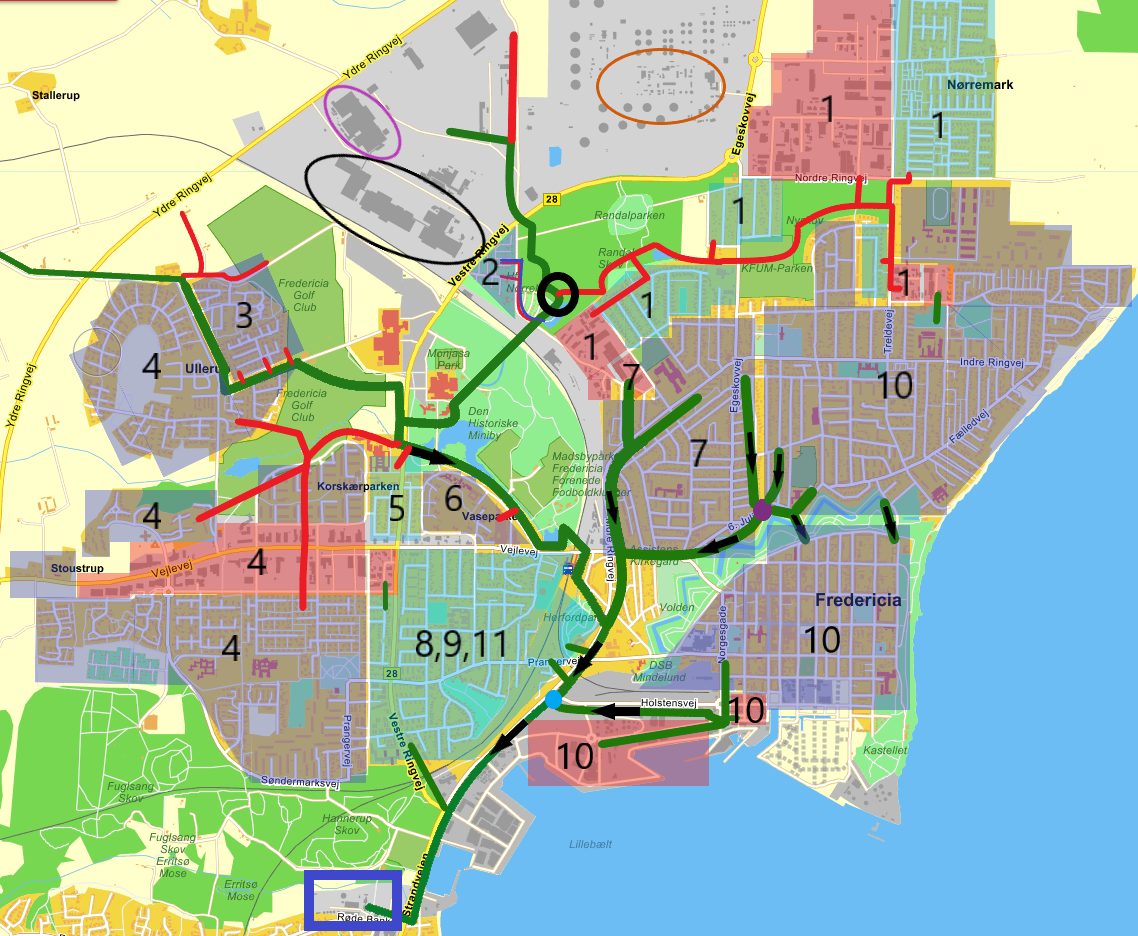
\includegraphics[width=1\textwidth]{report/system_overview/pictures/kloakgrid_simplified9.png}
\caption{Simplified mapping of the northern part of the sewer network in Fredericia. The two blue transparent colors indicate populated areas and the red transparent area indicate industry. Red and green lines is sewers with flows of wastewater and combined wastewater and surface runoff  respectively. Bottling plant, refinery and brewery is marked by purple, brown and black circles respectively. The black circle denotes the start point for the main sewer line. The green sewer line with an yellow line within it is the main sewer line. The purple dot is a connecting point with two incoming and two outgoing sewer lines. Blue dot is a wastewater pumping station which elevates sewage such that gravity can be utilized for the remaining transport into the treatment plant. Blue rectangle marks the location of the wastewater treatment plant.
%Mapping of part of the sewer network in Fredericia. The red and green lines indicate sewers where the red sewers has flows of sewage only and the green line is combined sewage and runoff from urban surfaces. Transparent parts indicate that the area has a connected sewer grid within and the red/green lines from this grid indicates the output from this area. Two shades of transparent blue is used to illustrate sewer systems in populated areas. The red transparent areas indicate minor industry and the black, brown and purple rings is brewery, refinery and bottling plant respectively. The purple dot indicate a splitting point with two incoming and outgoing sewer pipes. The light blue dot is a sewer reservoir before wastewater is led to the wastewater treatment plant indicated by the blue rectangle.
\cite{Krak} \cite{GIS_kort}}
\label{fig:kloakgrid_simplified}
\end{figure}


The various enumerated parts in figure \ref{fig:kloakgrid_simplified} is shown by order of attachment to the main sewer line, together with distance between each attachment, in figure \ref{fig:sewer_line_diagram}. 

\begin{figure}[H]
\centering
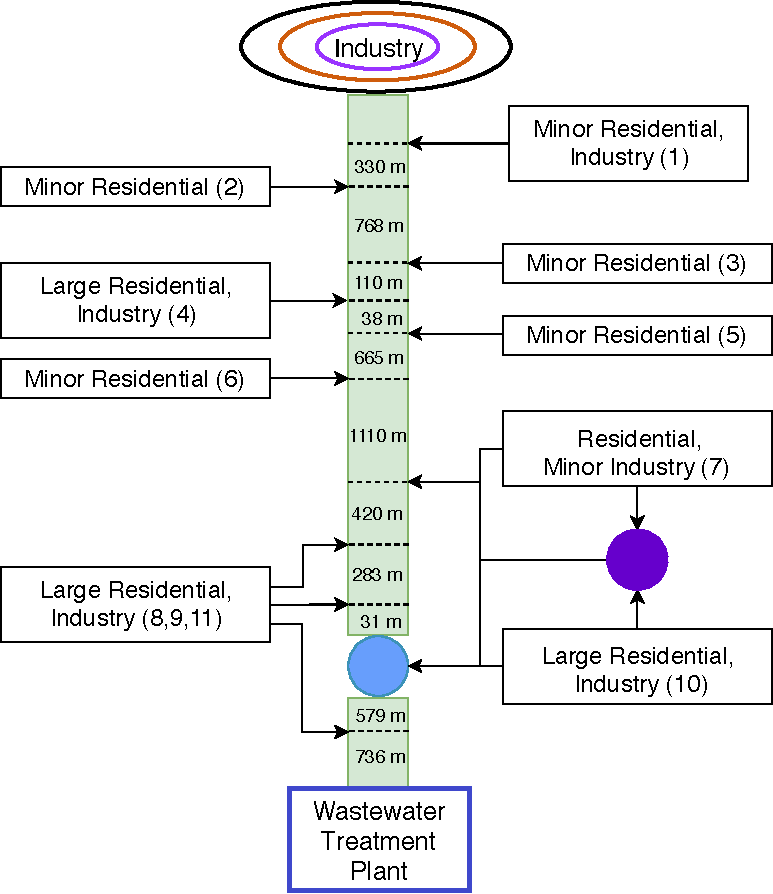
\includegraphics[width=0.6 \textwidth]{report/system_overview/pictures/sewer_line_diagram.pdf}
\caption{Simplification of the attachments to the main sewer line shown in figure \ref{fig:kloakgrid_simplified}. The numbers correspond to which area is connected to the main sewer line farthest from the wastewater treatment plant, with the distance between them \cite{GIS_kort}.}
\label{fig:sewer_line_diagram}
\end{figure}

Furthermore the different sections consist of pipe of varying diameters as can be seen in table \ref{tab:kloak_diameter}.

% \begin{table} 
% \centering
% \begin{tabular}[H]{|c|c|c|} \hline
% %\begin{table}[H]

% \multirow{2}{*}{Pipe section} & Pipe length & Inner pipe diameter \\ 
% 							  & (meter)		& (millimeter)		\\ \hline
% \multirow{2}{*}{1 $\rightarrow$ 2}		  & 303			  & 900	\\
% 						 & 27			  & 1000 \\ \hline
% 						 & 155			  & 1000 \\
% 2 $\rightarrow$ 3		 & 295			  & 800  \\
% 			 			 & 318			  & 900 \\ \hline
% 3 $\rightarrow$ 4		 & 110			  & 900 \\ \hline
% 4 $\rightarrow$ 5		 & 38 			  & 1000 \\ \hline
% 5 $\rightarrow$ 6		 & 665			  & 1000 \\ \hline
% \multirow{2}{*}{6 $\rightarrow$ 7}		 & 155			  & 1000 \\
% 			 			 & 955			  & 1200 \\ \hline
%  						 & 293			  & 1200 \\
% 7 $\rightarrow$ 8		 & 11 			  & 1300 \\
% 			 			 & 116			  & 1200 \\ \hline
% 8 $\rightarrow$ 9		 & 283			  & 1400 \\ \hline
% 9 $\rightarrow$ 10		 & 31			  & 1400 \\ \hline
% 						 & 125			  & 1600 \\
% 10 $\rightarrow$ 11	 	 & 94			  & 1500 \\
% 						 & 360 			  & 1600 \\ \hline
% 11 $\rightarrow$ WWTP    & 736			  & 1600 \\ \hline
% Total length 		     & \multirow{2}{*}{5070}  &		 \\ 
% 1 $\rightarrow$ WWTP     &						  & \\ \hline

% \end{tabular}

% \caption{Table of the various lengths and the approximate inner diameter of pipe, appearing in order, in the main sewer line. Pipe section indicate the length of pipe between the attachment of the various areas to the main sewer line.} 
% \label{tab:kloak_diameter}
% \end{table}


\begin{table} [H]
\centering
\begin{tabular}{|c|c|c|c|c|c|} 
\hline
\rowcolor[HTML]{9B9B9B} 
\multicolumn{1}{|c|}{\cellcolor[HTML]{9B9B9B}\textbf{Pipe section}} & \multicolumn{1}{c|}{\cellcolor[HTML]{9B9B9B}\textbf{\begin{tabular}[c]{@{}c@{}}Pipe length\\ (meter)\end{tabular}}} & \multicolumn{1}{c|}{\cellcolor[HTML]{9B9B9B}\textbf{\begin{tabular}[c]{@{}c@{}}Inner pipe\\ diameter (mm)\end{tabular}}} &
\multicolumn{1}{c|}{\cellcolor[HTML]{9B9B9B}\textbf{\begin{tabular}[c]{@{}c@{}}Bed datum\\ in (m)\end{tabular}}} & \multicolumn{1}{c|}{\cellcolor[HTML]{9B9B9B}\textbf{\begin{tabular}[c]{@{}c@{}}Bed datum\\ out (m)\end{tabular}}} & \multicolumn{1}{c|}{\cellcolor[HTML]{9B9B9B}\textbf{\begin{tabular}[c]{@{}c@{}}Bed\\ slope (\textperthousand)\end{tabular}}} \\ \hline
\multirow{2}{*}{1 $\rightarrow$ 2}		  & 303			  & 900    & 11,56  & 10,65 & 3,00\\
										 & 27			  & 1000   & 10,65  & 10,57 & 3,00 \\ \hline
										 & 155			  & 1000   & 10,57  & 9,94  & 4,10 \\
2 $\rightarrow$ 3						 & 295			  & 800    & 9,94   & 6,33  & 12,20 \\
			 							 & 318			  & 900    & 6,33   & 4,71  & 5,30 \\ \hline
3 $\rightarrow$ 4						 & 110			  & 900    & 4,71   & 4,31  & 3,60 \\ \hline
4 $\rightarrow$ 5						 & 38 			  & 1000   & 4,31   & 4,40  & -2,40 \\ \hline
5 $\rightarrow$ 6						 & 665			  & 1000   & 4,40   & 2,43  & 3,00 \\ \hline
\multirow{2}{*}{6 $\rightarrow$ 7}		 & 155			  & 1000   & 2,43   & 2,31  & 0,80 \\
			 							 & 955			  & 1200   & 2,31   & -0,48&  2,90 \\ \hline
 										 & 293			  & 1200   & -0,48  & unknown&  \\
7 $\rightarrow$ 8						 & 11 			  & 1300   & unknown& -1,38&  \\
			 							 & 116			  & 1200   & -1,38  & -1,62&  2,10\\ \hline
8 $\rightarrow$ 9						 & 283			  & 1400   & -1,62  & -2,09&  1,70\\ \hline
9 $\rightarrow$ 10						 & 31			  & 1400   & -2,09  & -2,15& 1,90 \\ \hline
										 & 125			  & 1600   & 0,31   & 0,05 & 2,10 \\
10 $\rightarrow$ 11	 	 				 & 94			  & 1500   & 0,05   & -0,07& 1,30\\
						 			 	 & 360 			  & 1600   & -0,07  & -1,72& 4,60 \\ \hline
11 $\rightarrow$ WWTP   				 & 736			  & 1600   & -1,72  & -2,60& 1,20\\ \hline
Total length 		    				 & \multirow{2}{*}{5070}  &	  & & & 	 \\ 
1 $\rightarrow$ WWTP    				 &						  &   & & & \\ \hline

\end{tabular}

\caption{Table of the various lengths and the approximate inner diameter of pipe, appearing in order, in the main sewer line. Pipe section indicate the length of pipe between the attachment of the various areas to the main sewer line \cite{GIS_kort}.} 
\label{tab:kloak_diameter}
\end{table}

Some assumptions is made to avoid complications during simulation. The negative slope of the section between connection point four and five is flipped such that no permanent storage of sewage happens. The reason for this assumption is that it will ease the computation, of the free flow in that section, if storage in the pipe sections could be disregarded during simulation. Furthermore the new slope is deemed acceptable based on the obtained slopes for the remaining pipe sections. 
For the two pipe sections between point seven and eight, where out- and input datum is unknown, are gathered in to a single pipe section. This section will be designated an inner diameter of 1200 mm as the section with the larger diameter is assumed insignificant for the free flow at the end points of the entire section.

\begin{table} [H]
\centering
\begin{tabular}{|c|c|c|c|} 
\hline
\rowcolor[HTML]{9B9B9B} 
\multicolumn{1}{|c|}{\cellcolor[HTML]{9B9B9B}\textbf{Pipe section}} & 
\multicolumn{1}{c|}{\cellcolor[HTML]{9B9B9B}\textbf{\begin{tabular}[c]{@{}c@{}}Pipe length\\ (meter)\end{tabular}}} & 
\multicolumn{1}{c|}{\cellcolor[HTML]{9B9B9B}\textbf{\begin{tabular}[c]{@{}c@{}}Inner pipe\\ diameter (mm)\end{tabular}}} &
\multicolumn{1}{c|}{\cellcolor[HTML]{9B9B9B}\textbf{\begin{tabular}[c]{@{}c@{}}Bed\\ slope (\textperthousand)\end{tabular}}} \\ \hline

4 $\rightarrow$ 5						& 38 			  & 1000   & 2,40 \\ \hline

\multirow{2}{*}{7 $\rightarrow$ 8}	 	& 304 			  & 1200   & 3.00  \\
			 							& 116			  & 1200   &   2,10\\ \hline

\end{tabular}
\caption{New slope values for sections with negative slope and unknown values.}
\label{tab:new_slope_values}
\end{table}


To simulate how the wastewater propagation throughout the sewer network the flows in each residential and industrial area needs to be known. However Fredericia does not have measurement of the flow from each area, they only have measurements at some pumping stations across the city. Therefore it is chosen to use the flow profile shown in figure \ref{fig:input_to_wwtp} for the residential areas, as an estimate of the flow across a day. This flow profile will be scaled to fit each residential area in figure \ref{fig:sewer_line_diagram}.

From figure \ref{fig:kloakgrid_simplified} it can be seen that 11 different flow profiles needs to constructed to cover each residential and industrial area. Each of these residential and industrial areas have been measured to give an estimate of the area for each zone. In table \ref{tab:size_of_areas} the size of the residential and industrial areas are shown. 

\begin{table}[H]
\centering
\begin{tabular}{|c|c|c|}
\hline
\textbf{Zone} & \textbf{\begin{tabular}[c]{@{}c@{}}Residential\\ area\\ $[km^2]$\end{tabular}} & \textbf{\begin{tabular}[c]{@{}c@{}}Industrial\\ area\\ $[km^2]$\end{tabular}} \\ \hline
1 - Thulesvej & 0,167                                                                        & 0,0083                                                                      \\ \hline
1 - Nørremark & 0,458                                                                        & 0,543                                                                       \\ \hline
2             & 0,056                                                                        & -                                                                           \\ \hline
3             & 0,167                                                                        & -                                                                           \\ \hline
4             & 1,872                                                                        & 0,375                                                                       \\ \hline
5             & 0,104                                                                        & -                                                                           \\ \hline
6             & 0,115                                                                        & -                                                                           \\ \hline
7             & 0,771                                                                        & 0,014                                                                       \\ \hline
8-9           & 0,667                                                                        & 0,021                                                                       \\ \hline
10            & -                                                                            & -                                                                           \\ \hline
11            & 0,278                                                                        & -                                                                           \\ \hline
\end{tabular}
\caption{Table over the size of the are different residential and industrial zones.}
\label{tab:size_of_areas}
\end{table}

By knowing the area and assuming that the density of the population is the same across the city, hence a flow profile can be scale to each of the residential and industrial areas. In figure \ref{fig:flow_profile_thulevej} a flow profile is shown for Thulesvej which is located in residential area one closet to the main sewer line. 

%Furthermore, from one of the pumping stations a measurement is obtained that illustrates the flow from that zone. This will be used to construct a flow profile according to the area that this pumping station is covering. 

\begin{figure}[H]
\centering
% This file was created by matlab2tikz.
%
%The latest updates can be retrieved from
%  http://www.mathworks.com/matlabcentral/fileexchange/22022-matlab2tikz-matlab2tikz
%where you can also make suggestions and rate matlab2tikz.
%
\definecolor{mycolor1}{rgb}{0.00000,0.44700,0.74100}%
%
\begin{tikzpicture}

\begin{axis}[%
width=4.521in,
height=1.7566in,
at={(0.758in,0.481in)},
scale only axis,
xmin=3600,
xmax=90000,
scaled x ticks = false,
xtick={3600,17950,32300,46650,61000,75350,89700},
xticklabels={{01:00},{05:00},{09:00},{13:00},{17:00},{21:00},{01:00},{},{},{}},
xlabel={Time [hh:mm]},
xmajorgrids,
ymin=-0.5,
ymax=7,
ylabel={$\text{Flow [m}^\text{3}\text{/hr]}$},
ymajorgrids,
axis background/.style={fill=white},
title style={font=\bfseries},
title={Daily flow},
legend style={legend cell align=left,align=left,draw=white!15!black}
]
\addplot [color=mycolor1,solid]
  table[row sep=crcr]{%
3599	0\\
3799	0\\
3998	0\\
4197	0\\
4396	0\\
4595	0\\
4794	0\\
4993	0\\
5192	0\\
5391	0\\
5590	0\\
5789	0\\
5988	0\\
6188	0\\
6387	0\\
6586	0\\
6785	0\\
6984	0\\
7183	0\\
7382	0\\
7581	0\\
7780	0\\
7979	0\\
8178	0\\
8377	0\\
8577	0\\
8776	0\\
8975	0\\
9174	0\\
9373	0\\
9572	0\\
9771	0\\
9970	0\\
10169	0\\
10368	0\\
10567	0\\
10766	0\\
10965	0\\
11165	0\\
11364	0\\
11563	0\\
11762	0\\
11961	0\\
12160	0\\
12359	0\\
12558	0\\
12757	0\\
12956	0\\
13155	0\\
13354	0\\
13554	0\\
13753	0\\
13952	0\\
14151	0\\
14350	0\\
14549	0.00710028180255936\\
14748	0.0184228250217605\\
14947	0.0320492223793003\\
15146	0.0482073693016751\\
15345	0.0671355323234623\\
15544	0.0890823640800493\\
15743	0.114306906530896\\
15942	0.143078582413403\\
16142	0.175851135929245\\
16341	0.212588195200944\\
16540	0.253744214191448\\
16739	0.299629869141819\\
16938	0.350565997430973\\
17137	0.406883518354036\\
17336	0.468923342131185\\
17535	0.537036267147258\\
17734	0.611582865421718\\
17933	0.692933356309431\\
18132	0.781467468431938\\
18331	0.877574289839258\\
18531	0.982195922443594\\
18730	1.09469519004965\\
18929	1.21599102593738\\
19128	1.3465082650137\\
19327	1.48668017480407\\
19526	1.63694823493869\\
19725	1.79776190486959\\
19924	1.96957837981796\\
20123	2.15286233495235\\
20322	2.34808565779734\\
20521	2.55572716887281\\
20720	2.77627233056388\\
20920	3.0114231889665\\
21119	3.25932816256334\\
21318	3.52163248137147\\
21517	3.79884505460662\\
21716	4.24535835961483\\
21915	4.68162393830136\\
22114	5.0605303399952\\
22313	5.38652724971494\\
22512	5.66385308888405\\
22711	5.89653976849929\\
22910	6.08841744227553\\
23109	6.24311925981753\\
23308	6.36408611977997\\
23508	6.45495440917018\\
23707	6.51789852026043\\
23906	6.55633849014062\\
24105	6.57299288668956\\
24175	6.57415203876262\\
24304	6.57041181650709\\
24503	6.55098167809271\\
24702	6.51692991498017\\
24901	6.4703297689161\\
25100	6.41310503299458\\
25299	6.3470348048595\\
25498	6.2737582398154\\
25697	6.19477930401627\\
25897	6.11104412197444\\
26096	6.02464281487946\\
26295	5.93629279768905\\
26494	5.84700423972142\\
26693	5.75767591081538\\
26892	5.66909993449537\\
27091	5.58196654112981\\
27290	5.4968688210775\\
27489	5.41430747787304\\
27688	5.33469558136816\\
27887	5.25836332089683\\
28086	5.18556275841323\\
28285	5.11647258168728\\
28485	5.0508846198317\\
28684	4.98950099222484\\
28883	4.93197089391124\\
29082	4.87822678626446\\
29281	4.82815154614999\\
29480	4.78158321907345\\
29679	4.73831977233886\\
29878	4.69812384820355\\
30077	4.66072751704663\\
30276	4.62583703052387\\
30475	4.59313757473281\\
30674	4.5622980233338\\
30874	4.53283158549684\\
31073	4.50468196016016\\
31272	4.4773467537562\\
31471	4.45047714751611\\
31670	4.42373179994733\\
31869	4.39678159999861\\
32068	4.36931442022513\\
32267	4.34103986992983\\
32466	4.31169404831157\\
32665	4.28104429767759\\
32864	4.24889395655103\\
33063	4.21508711284956\\
33263	4.17933000884771\\
33462	4.14191994481735\\
33661	4.1026777909942\\
33860	4.06165847677637\\
34059	4.01898147061914\\
34258	3.97483553325084\\
34457	3.92948347075326\\
34656	3.88397722505031\\
34855	3.87828619696292\\
35054	3.86930343292533\\
35253	3.85747628069986\\
35452	3.84321750420727\\
35651	3.8269069276083\\
35851	3.80879876200495\\
36050	3.78939405265094\\
36249	3.76889654705036\\
36448	3.74756974114895\\
36647	3.72565176386635\\
36846	3.70335676254554\\
37045	3.68087624735635\\
37244	3.65838039499861\\
37443	3.63601931223958\\
37642	3.61392425970557\\
37841	3.59220883690962\\
38040	3.57097012832554\\
38240	3.55018741982724\\
38439	3.53013612801473\\
38638	3.51076484830304\\
38837	3.49211525526681\\
39036	3.47421768422563\\
39235	3.45709205706402\\
39434	3.44074877307242\\
39633	3.42518956535756\\
39832	3.41040832363483\\
40031	3.39639188339584\\
40230	3.38312078275112\\
40429	3.37056998660284\\
40628	3.35870957943378\\
40828	3.34745071919719\\
41027	3.33686810559657\\
41226	3.32686310213515\\
41425	3.31739257121347\\
41624	3.30841150350928\\
41823	3.29987353111825\\
42022	3.29173141295388\\
42221	3.28393749256906\\
42420	3.27644412877175\\
42619	3.26920410036191\\
42818	3.26217098429212\\
43017	3.25529950899909\\
43217	3.24851217065511\\
43416	3.24183466319726\\
43615	3.23519285663449\\
43814	3.22854913912451\\
44013	3.22186845469703\\
44212	3.21511851496282\\
44411	3.20826998920971\\
44610	3.20129667325793\\
44809	3.19417563788733\\
45008	3.18688735701933\\
45207	3.17941581621549\\
45406	3.17174860242722\\
45606	3.16383689263074\\
45805	3.15575477699682\\
46004	3.14746198091052\\
46203	3.13896104857063\\
46402	3.13025830584381\\
46601	3.12136384673614\\
46800	3.11229150416268\\
46999	3.10305880603746\\
47198	3.09368691713768\\
47397	3.08420056695858\\
47596	3.07462796451394\\
47795	3.06500070041369\\
47994	3.05535363674715\\
48194	3.04567651271804\\
48393	3.03610730717207\\
48592	3.02664147037229\\
48791	3.01732563630324\\
48990	3.0082089940022\\
49189	2.99934311547402\\
49388	2.99078177508811\\
49587	2.98258076072152\\
49786	2.97479767731173\\
49985	2.96749174408537\\
50184	2.96072358490748\\
50383	2.95455501286881\\
50583	2.94902291968129\\
50782	2.94424641889452\\
50981	2.94026017220989\\
51180	2.93712849821384\\
51379	2.93491575689753\\
51578	2.9336861111075\\
51712	2.93344399692937\\
51777	2.93350328374416\\
51976	2.93443031534624\\
52175	2.9365293193663\\
52374	2.93986123720252\\
52573	2.94448559316272\\
52772	2.95046024994984\\
52971	2.95784116492597\\
53171	2.96673035011726\\
53370	2.97709054566539\\
53569	2.98901126884894\\
53768	3.00253844381405\\
53967	3.01771490395241\\
54166	3.03458016521482\\
54365	3.0531702045435\\
54564	3.07351724286139\\
54763	3.09564953469017\\
54962	3.11959116348308\\
55161	3.14536184343757\\
55360	3.17297672953474\\
55560	3.2025990174384\\
55759	3.23393799133826\\
55958	3.26713748554458\\
56157	3.30219265112997\\
56356	3.33909325560095\\
56555	3.37782354681432\\
56754	3.41836212902034\\
56953	3.46068185036243\\
57152	3.50474970132568\\
57351	3.55052672761426\\
57550	3.59796795453961\\
57749	3.64702232576993\\
57949	3.69789080473406\\
58148	3.75000107940876\\
58347	3.80353407849953\\
58546	3.85841406720561\\
58745	3.91455914615849\\
58944	3.97188128289352\\
59143	4.03028636135278\\
59342	4.08967424906017\\
59541	4.14993888181998\\
59740	4.21096836895186\\
59939	4.27264511666528\\
60138	4.33484597199087\\
60337	4.39744238646266\\
60537	4.460616902581\\
60736	4.52359842141341\\
60935	4.58655871601919\\
61134	4.64934970900322\\
61333	4.7118190777594\\
61532	4.77381055242879\\
61731	4.83516423899175\\
61930	4.89571696741947\\
62129	4.95530266351737\\
62328	5.01375274828578\\
62527	5.07089656280736\\
62726	5.12656181990029\\
62926	5.1808420410537\\
63125	5.23301961581908\\
63324	5.28319605858069\\
63523	5.33119764669666\\
63722	5.37685171215669\\
63921	5.41998726577409\\
64120	5.46043565259203\\
64319	5.49803123715681\\
64518	5.53261212032364\\
64717	5.56402088975496\\
64916	5.5921054013216\\
65115	5.61671959434555\\
65314	5.63772434100905\\
65514	5.65506542608248\\
65713	5.66844637033604\\
65912	5.67785054580365\\
66111	5.68317579333198\\
66265	5.6844393264031\\
66310	5.68433166094568\\
66509	5.68124046587969\\
66708	5.67383839505733\\
66907	5.66207664129223\\
67106	5.64592258155172\\
67305	5.62536099087637\\
67504	5.60039529730472\\
67703	5.57104887762718\\
67903	5.5371862865325\\
68102	5.49921381139279\\
68301	5.45706450861086\\
68500	5.41085544542991\\
68699	5.36073073781378\\
68898	5.30686309653841\\
69097	5.24945541691582\\
69296	5.18874241446603\\
69495	5.12499230152653\\
69694	5.05850851408906\\
69893	4.9896314807656\\
70092	4.91874043928682\\
70292	4.84588779072665\\
70491	4.77226660569418\\
70690	4.6980235194415\\
70889	4.62371235792628\\
71088	4.54993556513772\\
71260	4.48710030274668\\
71287	4.49353726057994\\
71486	4.44947345408763\\
71685	4.407048692502\\
71884	4.36625858371511\\
72083	4.32709083435589\\
72282	4.289525499708\\
72481	4.25353523389844\\
72680	4.21908554009987\\
72880	4.18597314726358\\
73079	4.15448091308838\\
73278	4.12438506605859\\
73477	4.09562497625584\\
73676	4.06813411464458\\
73875	4.04184030327419\\
74074	4.01666596530525\\
74273	3.99252837517106\\
74472	3.96933990887471\\
74671	3.94700829381207\\
74870	3.92543685921783\\
75069	3.9045247860968\\
75269	3.88406627795044\\
75468	3.86415709197283\\
75667	3.84458185304801\\
75866	3.82522563565619\\
76065	3.80597061808801\\
76264	3.78669633247073\\
76463	3.76727991501112\\
76662	3.74759635595384\\
76861	3.72751874991917\\
77060	3.70691854598326\\
77259	3.68566579766375\\
77458	3.66362941327093\\
77657	3.64067740596097\\
77857	3.61655366789701\\
78056	3.5913658514955\\
78255	3.56486291252174\\
78454	3.53691178579501\\
78653	3.50737976303432\\
78852	3.4761347426544\\
79051	3.44304548025224\\
79250	3.40798183840312\\
79449	3.37081503706588\\
79648	3.33141790363627\\
79847	3.28966512291887\\
80046	3.24543348750541\\
80246	3.19836004897266\\
80445	3.14879681142805\\
80644	3.09639967201374\\
80843	3.04105637174048\\
81042	2.98265801102665\\
81241	2.92109930000879\\
81440	2.85627880878449\\
81639	2.78809921741142\\
81838	2.71646756609606\\
82037	2.64129550526046\\
82236	2.56249954575803\\
82435	2.4800013090622\\
82635	2.39328459231101\\
82834	2.30314888751374\\
83033	2.20910864015839\\
83232	2.11110844635167\\
83431	2.0090992647929\\
83630	1.90303866671892\\
83829	1.79289108603862\\
84028	1.67862806962992\\
84227	1.56022852735244\\
84426	1.43767898193824\\
84625	1.31097381977632\\
84824	1.1801155402888\\
85023	1.04511500664776\\
85223	0.905282216762484\\
85422	0.762043980613217\\
85621	0.614748973653748\\
85820	0.463444062107368\\
86019	0.308185727662584\\
86218	0.149040317526378\\
86401	0\\
86417	0\\
86616	0\\
86815	0\\
87014	0\\
87213	0\\
87412	0\\
87612	0\\
87811	0\\
88010	0\\
88209	0\\
88408	0\\
88607	0\\
88806	0\\
89005	0\\
89204	0\\
89403	0\\
89602	0\\
90000	0\\
};
%\addlegendentry{Zone 1,1};

\end{axis}
\end{tikzpicture}%
\caption{A flow profile for Thulesvej.}
\label{fig:flow_profile_thulevej}
\end{figure}  \fxnote{skal tilpasse thulesvej, samt enheden skal selvfølgelig være m3/s}

From the data given by Fredericia WWTP, which can be seen in attachments /Data\_pump\_stations/Thulesvej-217, this flow profile have been constructed to fit a working day flow for Thulesvej. It has been chosen to only produce flow profiles for working days and therefore non of the profiles fits a weekend. This profile covers both the wastewater from the residential and industrial area at Thulesvej. The remaining flow profiles for the rest of the zones can be seen in appendix \fxnote{appendix mangler, samt en reference}. Furthermore, these flow profiles illustrates the input flow into the main sewer line, and therefore some of the flow profiles will have added a delay, due to longer transport time from the zone to the main sewer line. An explanation for each profile to a zone is given below.    

The residential areas denoted with one in figure \ref{fig:sewer_line_diagram}, stretch across a long sewer line. Where the sewage have to be transported a longer distance from the zone furthest away before reaching the main sewer line. It is therefore chosen to make two flow profiles, one from the residential and industrial area right next to the main sewer line, and one for the rest of the zones. These two flow profiles will be add together, and thereby the peaks will be extended for a longer period than a normal profile. The industrial area consists mainly of auto shops, recycle factory and workshops and therefore they will have the same flow profile as for residential area. 

From the second zone only one flow profile will be used and as the zone is close to main sewer line no delay in the profile is added. At zone three the distance from the residential area to the main sewer line is long, and therefore a delay will be added. The fourth zone covers a larger area and as some of the residential are far away from the main sewer line, therefore the flow profile is extended in the peaks. The industrial consists of grocery stores, workshops and car shops and therefore will have the same flow profile.

Zone five and six will have a normal profiles without delays. Zone seven will have a profile with delay as it also stretch across a long sewer line before reaching the main sewer line. Zone eight, nine and eleven will all have the same profile just scaled according to the size of the zones, and the industrial area is the same as the one in zone four. 

From zone ten a pump is pumping the wastewater to the main sewer line every 30 minuted for a period of 15 minutes. The pump has a pumping capacity of 0,350 $m^3/s$ which have been state by Fredericia. Therefore the flow profile for this area will be a constant input of 0,350 $m^3/s$ for 15 minutes every 30 minute.     

\chapter{System design}
\label{System_design}

%During the design of the system, the efficiency of the AVR is considered. As it is written, the main task of the AVR is to keep the voltage constant and therefore independent from the load on the genset. 

%Simulation results shows however, that there is a disturbance appearing on the voltage when the load changes. Therefore control can be applied to improve and correct the disturbance on the combined genset and inverter system. 
To correct the disturbance appearing when a change in load occurs to the combined genset and inverter system, control needs to be applied where the disturbance can be corrected.

In order to determine where control can be applied optimally, real world power measurements of a genset and an inverter is shown on \figref{fig:gensetPowermeas} and \figref{fig:inverter10kwstep}


\begin{figure}[H]
\centering
%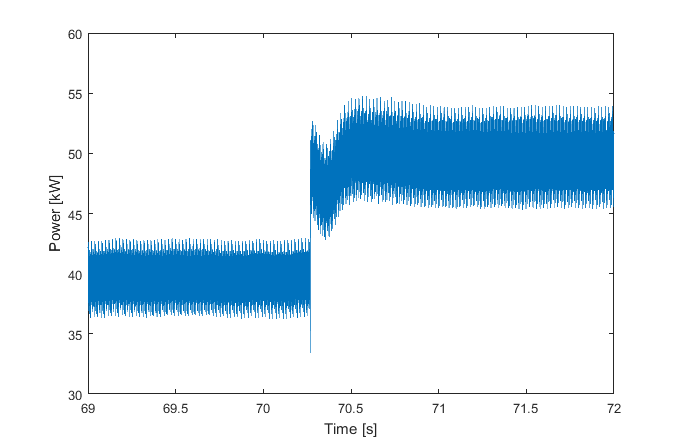
\includegraphics[width=0.8\textwidth]{rapport/billeder/4050kwstep.png}
% This file was created by matlab2tikz.
%
%The latest updates can be retrieved from
%  http://www.mathworks.com/matlabcentral/fileexchange/22022-matlab2tikz-matlab2tikz
%where you can also make suggestions and rate matlab2tikz.
%
\definecolor{mycolor1}{rgb}{0.00000,0.44700,0.74100}%
%
\begin{tikzpicture}

\begin{axis}[%
width=4.0in,
height=3.0in,
at={(0.758in,0.481in)},
scale only axis,
xmin=69,
xmax=72,
xlabel={Time [s]},
xmajorgrids,
ymin=30,
ymax=60,
ylabel={Power [kW]},
ymajorgrids,
axis background/.style={fill=white}
]
\addplot [color=mycolor1,solid,forget plot]
  table[row sep=crcr]{%
69	42.0960090642869\\
69.00238	42.5559127479842\\
69.00448	36.9304035360587\\
69.00788	36.6986566116855\\
69.0092	41.9040380689165\\
69.01452	36.3199030238924\\
69.0198	42.7008963276288\\
69.02228	42.4192813188401\\
69.02452	37.0509363491857\\
69.02918	41.9996463688265\\
69.03454	36.3947483400785\\
69.03458	36.4410586652751\\
69.03918	42.7221469649957\\
69.04236	42.3933520014313\\
69.04792	36.6963423109946\\
69.0499	41.8899368936894\\
69.05454	36.4234595826002\\
69.05786	37.3699294333512\\
69.05916	42.6899957342084\\
69.06226	42.4038924677669\\
69.06788	36.6999047397127\\
69.07238	41.8721813488837\\
69.07456	36.2972837091461\\
69.0778	37.4358016851034\\
69.07922	42.7229193761768\\
69.0831	42.1095546802261\\
69.0879	36.6864335616395\\
69.09234	41.9090754786125\\
69.09454	36.3530078466834\\
69.09788	37.4736333563494\\
69.09924	42.803456752\\
69.10788	36.8654118284957\\
69.1092	42.053927176649\\
69.11236	41.8526943259543\\
69.1146	36.487117478319\\
69.11916	42.8016329754773\\
69.12444	37.1177209561857\\
69.12794	36.79171310045\\
69.12988	42.0205814942576\\
69.1324	41.954159768411\\
69.13454	36.5077477883357\\
69.13922	42.8079391245626\\
69.14452	37.0621687492813\\
69.14788	36.8206470621655\\
69.14924	41.9535676146947\\
69.15454	36.4610679948756\\
69.159	42.6757066554406\\
69.1592	42.9818657293557\\
69.16448	37.0721743774901\\
69.16792	36.786152688155\\
69.1724	42.0061495743427\\
69.17454	36.4569230249899\\
69.1792	42.915073892547\\
69.17978	42.8051384911361\\
69.18446	37.1797525446474\\
69.18794	36.9837290386078\\
69.1892	42.1755218118723\\
69.19458	36.5808635386711\\
69.1992	42.8726922139985\\
69.20236	42.5029991764865\\
69.2045	36.9679436405511\\
69.2079	36.7118718139959\\
69.20916	42.0321879179646\\
69.21454	36.4941907596754\\
69.21976	42.8314160043567\\
69.22228	42.5236552886485\\
69.22794	36.8211016657531\\
69.23232	41.9880176153725\\
69.23456	36.3773625124651\\
69.23784	37.5166323154776\\
69.23916	42.8174871562231\\
69.24232	42.590353934823\\
69.24788	36.7503466947837\\
69.25226	41.9948603146254\\
69.25454	36.4288644289047\\
69.25782	37.5208282942826\\
69.25912	42.8203444510937\\
69.26304	42.110040536459\\
69.26786	36.824783134485\\
69.26978	41.9860289022677\\
69.27454	36.4985082200892\\
69.2778	37.388844183683\\
69.27912	42.8050592828384\\
69.2879	36.7534873638932\\
69.28916	41.9644014044407\\
69.29228	41.8569769949865\\
69.2945	36.4587110791705\\
69.29784	37.4018825436509\\
69.29912	42.7001597566365\\
69.30786	36.7372144598477\\
69.30912	41.8394833021144\\
69.31232	41.9174742451826\\
69.31446	36.407544666765\\
69.31914	42.77189820798\\
69.32448	36.8780068976299\\
69.32786	36.6577634656352\\
69.3298	41.8818526132918\\
69.33238	41.9412082546322\\
69.33452	36.3830499324044\\
69.3391	42.7921672914878\\
69.34446	37.0097091863565\\
69.34788	36.8212195523597\\
69.34918	42.0316253352224\\
69.35446	36.5085142398206\\
69.35914	42.8028840999977\\
69.35978	42.7308984749884\\
69.36446	36.8317367049195\\
69.36784	36.6425410625091\\
69.36986	41.93765235963\\
69.37454	36.4997869016355\\
69.37918	42.7663234961048\\
69.3823	42.4607232735905\\
69.38446	36.9269220451554\\
69.3879	36.7404906274645\\
69.39238	41.9457678173549\\
69.39452	36.4035279290206\\
69.39916	42.8613109897251\\
69.40236	42.5040022099868\\
69.40782	36.6954435348295\\
69.41236	41.9242553436566\\
69.41452	36.4317646157955\\
69.41476	37.0588116662464\\
69.41918	42.8055489910929\\
69.42226	42.4343695662523\\
69.42788	36.8109381920963\\
69.42922	41.9893380110246\\
69.43456	36.5288328574307\\
69.4378	37.4111151810318\\
69.43914	42.8096294189846\\
69.4424	42.2350981400335\\
69.44794	36.6461690103002\\
69.4499	41.979658643863\\
69.45452	36.6182238286659\\
69.4578	37.5080650981595\\
69.45918	42.8559135535829\\
69.46314	42.0411276929031\\
69.46788	36.7851028227498\\
69.47226	42.118916774762\\
69.47454	36.5688613736583\\
69.4778	37.6250868880573\\
69.47918	42.9697407046519\\
69.48794	36.7646662185471\\
69.48986	42.0351962137481\\
69.49236	42.0361810071846\\
69.49454	36.5193737098206\\
69.49916	42.8620786088031\\
69.50446	37.0578649575612\\
69.50788	36.7793626852272\\
69.50922	42.0225589214941\\
69.51238	41.8944825193229\\
69.5145	36.5327212654563\\
69.51912	42.8688581051802\\
69.52444	36.8543179818252\\
69.5279	36.6547344981785\\
69.52916	41.9774191997382\\
69.53456	36.6068834346194\\
69.53916	42.7941129209847\\
69.53974	42.7837982394699\\
69.54452	36.9256417413792\\
69.5479	36.7050533784797\\
69.55232	42.0417907518976\\
69.55454	36.4637929455961\\
69.55914	42.895415486223\\
69.56236	42.5572723675891\\
69.5645	36.8584055010284\\
69.56784	36.6438912346442\\
69.57236	41.9988491640251\\
69.57452	36.5215951636116\\
69.57912	42.9030254298698\\
69.58226	42.4721688147962\\
69.58448	37.034132909233\\
69.5892	42.0190249373194\\
69.59446	36.6333491906225\\
69.59452	36.5982302821719\\
69.59914	42.8737160126058\\
69.60234	42.4063261330556\\
69.60786	36.6724513371134\\
69.61236	41.9903464607732\\
69.61454	36.6102046278257\\
69.61774	37.5731619716849\\
69.61918	42.8226545773196\\
69.62226	42.4460644797842\\
69.62786	36.7232732693329\\
69.63226	42.0212667813456\\
69.63452	36.4991020600841\\
69.6378	37.5741224595183\\
69.63908	42.8657702982625\\
69.64308	42.1533547120755\\
69.64784	36.7065393692507\\
69.65226	41.9918094850021\\
69.6545	36.4806024986324\\
69.65776	37.5760328326756\\
69.65916	42.8587972534398\\
69.6678	36.8337109058741\\
69.66914	42.0196817592662\\
69.67226	41.9535243730622\\
69.67452	36.5865079747009\\
69.67908	42.8851210679419\\
69.68434	37.0164445499283\\
69.68784	36.6608366574602\\
69.68984	41.9880457954753\\
69.69236	41.8906351024035\\
69.69446	36.6019866596949\\
69.69912	42.8403754795681\\
69.70444	37.0022050329855\\
69.70786	36.7768392610297\\
69.70914	41.9176533135105\\
69.71448	36.4810131862259\\
69.7189	42.4050407810376\\
69.71908	42.8068381370481\\
69.72444	36.9350586779022\\
69.72788	36.7373228123708\\
69.73222	41.9812202700803\\
69.73452	36.4482173644258\\
69.73914	42.8121520067398\\
69.73972	42.7135639428442\\
69.74444	37.0044698724979\\
69.74782	36.7570272666854\\
69.74916	41.9263731958314\\
69.75448	36.4305931426707\\
69.75908	42.7642749899312\\
69.7623	42.329544517957\\
69.76446	36.8039268639819\\
69.76782	36.6717828391125\\
69.76916	41.8965328448592\\
69.7745	36.4979571222339\\
69.77912	42.6639264703874\\
69.78226	42.3699744944883\\
69.78786	36.6961571853764\\
69.7923	41.8776065753919\\
69.79452	36.364257480237\\
69.79778	37.4123091368669\\
69.79914	42.714239762884\\
69.80234	42.5033927383611\\
69.80782	36.6428529438385\\
69.81224	41.8693333666181\\
69.8145	36.303175864263\\
69.81774	37.4123313761866\\
69.81916	42.7569423768142\\
69.82302	42.0705679621064\\
69.82782	36.7724567682369\\
69.82976	41.9534202542857\\
69.83448	36.455942944107\\
69.83772	37.3257198163572\\
69.8391	42.7341242785117\\
69.84786	36.6695134425217\\
69.84974	41.9192503473183\\
69.85228	41.8234992149201\\
69.85448	36.4379300577773\\
69.85778	37.3533376711531\\
69.85916	42.6520996667939\\
69.8678	36.7561284869509\\
69.86914	41.8756984544379\\
69.8723	41.8753398842983\\
69.87448	36.2689492537303\\
69.87906	42.673723185013\\
69.88444	36.9482302550381\\
69.88782	36.6794774124858\\
69.88978	41.8730640727767\\
69.89226	41.8227102790494\\
69.89446	36.299687826756\\
69.8991	42.6791835505121\\
69.90444	37.0054999908332\\
69.90782	36.7685965083308\\
69.90916	41.9177155668194\\
69.91446	36.3318083734199\\
69.9191	42.7692211022521\\
69.91974	42.6682597928314\\
69.92444	36.9583777985286\\
69.92782	36.7610511912757\\
69.92916	41.9777344976742\\
69.93444	36.4694139772641\\
69.93972	42.7071721658007\\
69.94226	42.5203160639268\\
69.9444	37.040660311027\\
69.94782	36.8009511791569\\
69.95236	41.9439478633753\\
69.95452	36.3533483033263\\
69.95914	42.8359017849269\\
69.96234	42.6233830320923\\
69.96776	36.8665328345388\\
69.96984	41.8724544675611\\
69.97448	36.3520956009231\\
69.97468	36.8060974517473\\
69.97912	42.8304582964292\\
69.98228	42.5371843267494\\
69.98782	36.8442465988498\\
69.9891	41.9757908000066\\
69.99448	36.3964010888729\\
69.9978	37.4176116882202\\
69.99908	42.8177555747184\\
70.00232	42.484527445938\\
70.00786	36.7113305992732\\
70.00984	41.8856763746872\\
70.0145	36.4156829239612\\
70.01782	37.3991650847187\\
70.0197	42.7336589990408\\
70.02314	42.0755950250889\\
70.02782	36.7151396052684\\
70.03228	41.8643233127954\\
70.03452	36.2389573116088\\
70.03778	37.3723718319427\\
70.03912	42.7285120506424\\
70.04788	36.6496405318085\\
70.04914	41.793721201515\\
70.0523	41.7963466234005\\
70.05452	36.2534007846297\\
70.05918	42.7783813058802\\
70.06444	37.0672784807627\\
70.0679	36.765071488122\\
70.06918	41.901030034585\\
70.07228	41.6752178202025\\
70.07454	36.2889092215104\\
70.07918	42.7296110069536\\
70.08444	36.9184431859163\\
70.08788	36.6537777013455\\
70.08922	41.8198808324584\\
70.0945	36.3479600766345\\
70.0991	42.7096092634951\\
70.10446	36.9846087586051\\
70.10782	36.7112646769021\\
70.1123	41.8483568369744\\
70.11456	36.2573770911153\\
70.11914	42.7770127146621\\
70.1223	42.6296559544271\\
70.12448	36.9821079937539\\
70.12788	36.6300343687272\\
70.12982	41.7976287282342\\
70.13454	36.2420937164587\\
70.13916	42.7871454197887\\
70.1423	42.533514984814\\
70.14442	37.1082496000103\\
70.14912	41.9265248766925\\
70.1544	36.4299458695279\\
70.15444	36.3175826285389\\
70.1591	42.75221349622\\
70.16232	42.4511792064021\\
70.16786	36.6731747832976\\
70.16914	41.8915582455588\\
70.17448	36.4204421342659\\
70.17776	37.4405341217313\\
70.17916	42.8228488278424\\
70.18226	42.5801851776344\\
70.18784	36.7604632167825\\
70.1923	41.9403646247269\\
70.19454	36.3555067638187\\
70.19776	37.5714972191957\\
70.1991	42.8752468482219\\
70.20312	42.292661758565\\
70.20788	36.7628987651489\\
70.2098	41.900182952876\\
70.21446	36.3630673153674\\
70.21776	37.5400264214233\\
70.21914	42.9327582937706\\
70.2278	36.8665092742814\\
70.22916	42.0076093979571\\
70.23224	41.7879450409198\\
70.23446	36.4638425430387\\
70.2391	42.9061895585622\\
70.24426	37.3739368537502\\
70.24784	36.756891812381\\
70.24914	41.9703978986432\\
70.25236	41.8643394481613\\
70.25452	36.4757961823336\\
70.25914	42.8340255801467\\
70.26444	37.0901425588157\\
70.26712	33.4333518715314\\
70.2701	51.0612878172907\\
70.27442	45.0270296557091\\
70.27682	52.0299781725829\\
70.27996	52.6370796498976\\
70.28452	45.4213424162415\\
70.28794	44.6237789459264\\
70.29016	51.415011874031\\
70.29466	44.3580493103096\\
70.29936	51.5584043448115\\
70.29996	52.3206350845798\\
70.30472	44.8785884544262\\
70.30814	44.041840018107\\
70.31022	50.7605625085435\\
70.31492	43.6763221523153\\
70.32018	51.5075105455175\\
70.32032	51.3829253849544\\
70.32496	44.0128361249953\\
70.32838	43.3254468917184\\
70.3305	50.0694149513089\\
70.33518	43.1232268968911\\
70.34042	50.9410201240271\\
70.34392	50.3253953211744\\
70.34524	43.6762499398367\\
70.34868	43.1052248172896\\
70.35084	49.5799595597726\\
70.3555	42.8578169457409\\
70.36076	50.7819782570496\\
70.36432	50.4067160630674\\
70.36556	43.606190474468\\
70.3691	43.1134425602216\\
70.37114	49.7741295280009\\
70.37582	43.0844331900038\\
70.38116	51.1493496309611\\
70.38466	50.7323737407894\\
70.38942	43.6363414286325\\
70.38948	43.5610609514674\\
70.39156	50.2168431668401\\
70.39634	43.9556051350353\\
70.40168	51.8677379148232\\
70.40512	51.2971696856992\\
70.4099	44.0849771804608\\
70.41016	44.6863176272748\\
70.41538	51.1031476588399\\
70.42012	45.7436161754844\\
70.4221	52.7617468270531\\
70.4256	52.051468648218\\
70.43046	44.6920663529853\\
70.43584	51.7687343198908\\
70.43722	45.1753983882474\\
70.4406	46.4681780780348\\
70.44264	53.3524229498904\\
70.44614	52.8463425475193\\
70.45096	45.297907407443\\
70.45644	52.5797504900231\\
70.4578	45.7513244890023\\
70.4612	47.0941907068898\\
70.46318	53.9448211026162\\
70.46664	53.3498162768413\\
70.4715	45.7905099944217\\
70.47696	52.9290799038313\\
70.4783	46.1417471975033\\
70.48176	47.1715338491421\\
70.48376	54.3076377929939\\
70.48732	53.3087210867324\\
70.49214	45.7036512918599\\
70.49754	53.0939652307264\\
70.49894	46.4921270408411\\
70.50234	47.3220693284716\\
70.50434	54.5801847824257\\
70.50784	53.5357680014059\\
70.51268	45.9817782959345\\
70.51814	53.1780776438423\\
70.51954	46.3042209255278\\
70.52296	47.557876400469\\
70.52496	54.5104504956446\\
70.52842	53.8084588406305\\
70.53334	46.0505475641449\\
70.53878	53.474135757836\\
70.54016	46.3291178845373\\
70.54554	54.5761580493906\\
70.54702	47.6685151766476\\
70.54906	53.9946394665389\\
70.55394	46.2765422060897\\
70.5593	53.4605161624306\\
70.56076	46.5471472561103\\
70.56616	54.7370809573415\\
70.5676	47.5242556654587\\
70.56964	53.7100069786024\\
70.57452	46.048206073811\\
70.5799	53.3642183835991\\
70.58136	46.5870739632439\\
70.58474	47.3738460134918\\
70.58676	54.7811459105041\\
70.5902	53.5741387458698\\
70.59512	46.0162184950858\\
70.60044	53.2689257670258\\
70.60192	46.3407001039976\\
70.60526	47.4838924597703\\
70.6073	54.4591865949604\\
70.61076	53.728757906489\\
70.61564	45.995902235353\\
70.62248	46.2101188146408\\
70.62442	53.4178719597936\\
70.62776	54.4665928610968\\
70.6293	47.4830182607215\\
70.63138	53.7553171972382\\
70.63614	46.1953934157764\\
70.64156	53.4171777168288\\
70.643	46.4713864214292\\
70.64636	47.3768712027847\\
70.64832	54.6002975744565\\
70.65666	45.8569787963197\\
70.65884	53.1335981567439\\
70.66344	46.458594163468\\
70.6654	53.3697027612792\\
70.66686	47.2460673257569\\
70.66878	54.6142378771633\\
70.67714	45.9288887794314\\
70.67916	52.9213374657093\\
70.68394	46.1384706541846\\
70.68598	53.4896855512499\\
70.6873	47.3767854949597\\
70.68922	54.3032857271693\\
70.69754	45.9856948182314\\
70.69968	52.7660264259117\\
70.7029	53.4712901047816\\
70.70436	46.1638417997717\\
70.7097	54.4434781959212\\
70.7143	47.2733834995909\\
70.71794	46.0634317883033\\
70.71994	53.0916339012504\\
70.72332	53.183397416083\\
70.72472	46.3679717648648\\
70.73006	54.6456812078542\\
70.73486	46.6017512488447\\
70.73832	45.7060870112994\\
70.74036	53.059097481874\\
70.74506	46.2518721969053\\
70.7471	53.3391132704582\\
70.75038	54.361081973192\\
70.75524	46.3817388956859\\
70.75864	45.7970685573912\\
70.76066	52.6545703831312\\
70.7654	45.9109058804537\\
70.76742	53.2095452892685\\
70.77068	54.1948604126283\\
70.77548	46.3621983123932\\
70.77896	45.7759002862416\\
70.78094	52.6828063269633\\
70.78568	46.0245537717798\\
70.79034	53.7257682896201\\
70.79088	54.3422643429994\\
70.79576	46.578120088384\\
70.79922	45.8312285475219\\
70.80118	52.9070097043879\\
70.80596	46.163135245419\\
70.81108	54.1259960074531\\
70.81118	54.3399655847597\\
70.81594	46.370086974186\\
70.81938	45.7072377065637\\
70.82474	52.9720049111994\\
70.8261	46.0348100332574\\
70.83136	54.2607443313268\\
70.83476	53.4765411760567\\
70.83612	46.3409434972265\\
70.83962	45.6858143360648\\
70.84484	52.8878387832955\\
70.8463	45.821731262282\\
70.8515	54.0868203392586\\
70.85496	53.4425537299104\\
70.85622	46.2893706910563\\
70.85974	45.5612079733088\\
70.86498	52.8882747486843\\
70.86644	45.7693331176533\\
70.8716	54.1204405474887\\
70.87504	53.4006889979986\\
70.8798	45.7267285306345\\
70.88506	52.8151350209591\\
70.88646	45.8803454051915\\
70.88976	46.8893219738248\\
70.89172	54.1289831019751\\
70.89522	53.2125391039367\\
70.89984	45.5363517421172\\
70.902	52.8752164079188\\
70.90658	45.8760425090686\\
70.90982	46.8630037113443\\
70.91176	53.9865188452069\\
70.91512	53.1723407594623\\
70.9199	45.5343328152526\\
70.9266	45.6081575584656\\
70.9286	52.8111042707701\\
70.92984	46.9075678156745\\
70.93178	53.8425325440476\\
70.9355	52.8444890512657\\
70.93996	45.4385480618212\\
70.94656	45.6980239149082\\
70.94872	52.8882699966355\\
70.94984	46.9055728687006\\
70.95174	53.9704814822403\\
70.95994	45.6019429247602\\
70.96206	52.7520019525097\\
70.96656	45.7251724898296\\
70.96866	52.8450416537913\\
70.97172	53.9029444009135\\
70.97648	46.0945817472229\\
70.97988	45.4944010977029\\
70.98204	52.7986397507548\\
70.9865	45.7987218283703\\
70.98858	52.8380118482897\\
70.99168	53.8662395758284\\
70.99648	46.1781583892232\\
70.99986	45.4871108204855\\
71.00196	52.5812407753444\\
71.00652	45.6119390277517\\
71.01154	53.5642499406528\\
71.01166	53.8755023989569\\
71.01638	46.1930321984351\\
71.01978	45.5102786457739\\
71.02506	52.7751795374079\\
71.02644	45.666844549586\\
71.03162	53.8204830261127\\
71.035	53.2166341297505\\
71.03636	46.2295441526076\\
71.03976	45.5867395357371\\
71.04184	52.6738603948888\\
71.04638	45.650931677116\\
71.0516	53.8317166394311\\
71.05504	53.0551145567429\\
71.05966	45.4552626139033\\
71.06184	52.8988746667906\\
71.06632	45.702507006692\\
71.06958	46.6774869894146\\
71.0715	53.7784324843029\\
71.07494	53.0653782256745\\
71.07964	45.4515267155651\\
71.08484	52.5988589124266\\
71.08626	45.5598736672088\\
71.08948	46.7900686135001\\
71.09136	53.7262798437442\\
71.09486	53.3126747061282\\
71.09956	45.4126530847545\\
71.10618	45.5812691548811\\
71.10826	52.8313134363347\\
71.10942	46.7704094006248\\
71.1114	53.775489125655\\
71.11942	45.5805132050611\\
71.12148	52.7039878462102\\
71.1261	45.6762864177441\\
71.12826	52.7666402185948\\
71.13126	53.8183865067846\\
71.13594	46.1676705503499\\
71.13934	45.4510834156985\\
71.14148	52.8505507288321\\
71.14598	45.7880589007258\\
71.14812	52.8728054102785\\
71.15114	53.8554514106023\\
71.1559	46.1890533353317\\
71.15928	45.4875206927114\\
71.16144	52.6010246977267\\
71.16592	45.6383539910224\\
71.17054	53.1326230870118\\
71.17112	53.8298457471931\\
71.1758	46.2639093163582\\
71.1792	45.5457551969846\\
71.18138	52.7703770438821\\
71.18584	45.7619325017938\\
71.19104	53.9710059911579\\
71.19126	53.6005547822995\\
71.19568	46.328592518036\\
71.19916	45.6422609399174\\
71.2011	52.7916659502918\\
71.20574	45.7495074352876\\
71.21092	53.8242368660776\\
71.21434	53.1105267545364\\
71.21892	45.8014730331351\\
71.21906	45.5375154027807\\
71.22122	52.8863051217464\\
71.22584	46.1162649437828\\
71.23082	53.7847107447256\\
71.23424	52.9998205496609\\
71.23902	45.4215595723371\\
71.24416	52.5778840397923\\
71.24564	45.5963351028877\\
71.25076	53.7523653072162\\
71.25226	46.8153623547406\\
71.25428	53.228351465265\\
71.25888	45.4089775335227\\
71.26416	52.7226505906436\\
71.26552	45.5804281443879\\
71.26878	46.8440569700461\\
71.27068	53.7983085410215\\
71.27422	53.1670421717814\\
71.27878	45.5776362640795\\
71.28542	45.697043742227\\
71.2876	52.7739070520813\\
71.28872	46.7123560619483\\
71.29066	53.8404692782426\\
71.2987	45.455341253429\\
71.30082	52.967622311168\\
71.30534	45.8341020324545\\
71.3075	53.0162246513311\\
71.31054	53.9218924139003\\
71.31522	46.2004990300383\\
71.31864	45.5837536934881\\
71.32078	52.7494812496192\\
71.3253	45.7367725811661\\
71.32728	53.0100687352494\\
71.33046	53.8583271865866\\
71.33514	46.1856147666826\\
71.33854	45.4951831614787\\
71.34076	52.809506645643\\
71.3452	45.739567552735\\
71.35026	53.74352230674\\
71.35034	53.9433276684657\\
71.35506	46.236207372945\\
71.35848	45.653496394306\\
71.36062	52.7951805276131\\
71.36512	45.7759925223722\\
71.37026	53.8794699046798\\
71.37376	53.1044121280087\\
71.37498	46.0806476844957\\
71.37844	45.4868144744202\\
71.38058	52.9282167531453\\
71.38502	45.8503500080722\\
71.39028	53.7718272174376\\
71.39366	53.0253042356665\\
71.39838	45.4594464350904\\
71.40354	52.6916534151757\\
71.40502	45.6852258456259\\
71.4102	53.7071814641592\\
71.4116	46.8211955279325\\
71.41358	53.2477445173588\\
71.41832	45.3907465967294\\
71.4235	52.7373899113007\\
71.42494	45.6889670158353\\
71.43008	53.7636343634088\\
71.43158	46.8197989979884\\
71.43352	53.1012451632762\\
71.43824	45.5120156820241\\
71.4449	45.7741150182542\\
71.44686	52.8660004480151\\
71.44816	46.788708962806\\
71.45008	53.8548757857459\\
71.45822	45.3392168913569\\
71.46038	52.8192970747851\\
71.46482	45.8215205009855\\
71.46696	52.9485101794179\\
71.47004	53.8307051121251\\
71.47468	46.0800369319881\\
71.47818	45.3470706526821\\
71.48038	52.5090702706056\\
71.48484	45.7550091254727\\
71.48692	53.011094034409\\
71.49004	53.7751845303762\\
71.49476	46.0171126873648\\
71.4981	45.345935350152\\
71.50032	52.6876271171174\\
71.50478	45.8388496800331\\
71.50694	53.0939826428947\\
71.50996	53.9490689864845\\
71.51466	46.2266381174789\\
71.5181	45.598964319369\\
71.52022	52.8251470352419\\
71.5248	45.9630681901844\\
71.52994	53.975312020931\\
71.52998	53.9192777078161\\
71.53464	46.0658678056462\\
71.5381	45.4759350071745\\
71.54024	52.9278236844977\\
71.54476	45.9469327005668\\
71.54998	53.9781367845431\\
71.55334	53.0216023359351\\
71.55464	46.0672247166272\\
71.55806	45.4302100667347\\
71.56332	52.7960673500643\\
71.5647	45.7884692867009\\
71.5699	53.8735089682672\\
71.57342	53.2626210893572\\
71.57808	45.3630081685931\\
71.58328	52.7973478406942\\
71.58472	45.7446393374658\\
71.5899	53.85229132014\\
71.5914	46.8677891739702\\
71.59332	53.0964144548605\\
71.59808	45.4913139733374\\
71.6033	52.6933883883415\\
71.60474	45.8076804813001\\
71.60994	53.8726274516012\\
71.61144	46.7863236137181\\
71.61334	52.8617153136903\\
71.61806	45.3502748719974\\
71.62468	45.9635046382304\\
71.62668	53.0382351511764\\
71.628	46.9089211281453\\
71.6299	53.9494289280146\\
71.63804	45.461042109999\\
71.6402	52.6431118216925\\
71.64474	45.8141150403477\\
71.6468	53.1759775123072\\
71.64996	53.883022460981\\
71.6514	46.8879095506741\\
71.65804	45.4463659609614\\
71.66018	52.7264287046177\\
71.6647	45.8599489824402\\
71.66692	53.1242565937357\\
71.66998	53.979935575924\\
71.67466	46.1881184604331\\
71.6781	45.55271791248\\
71.68014	52.7041392725163\\
71.68468	45.8762577926624\\
71.6869	52.9409578377688\\
71.68994	53.9523136969509\\
71.69466	46.0751005557795\\
71.6981	45.4371906940874\\
71.70028	52.8665951301647\\
71.70474	45.9454504243325\\
71.70942	53.1604039981791\\
71.70992	53.9223473031121\\
71.7147	46.0774081679726\\
71.71806	45.4407000625245\\
71.72336	52.7221376039639\\
71.72476	45.7302012615513\\
71.73004	53.8099730197797\\
71.7334	53.2686401201852\\
71.73472	46.0269367833876\\
71.73812	45.4335099851671\\
71.74346	52.7873092892084\\
71.7448	45.7293354849006\\
71.75	53.9497010490111\\
71.75348	53.231161124839\\
71.7581	45.62922828975\\
71.75814	45.5335702763121\\
71.76026	52.7145111114315\\
71.765	46.2451881997123\\
71.77002	53.9196814621306\\
71.77342	53.0470056053912\\
71.77818	45.4631350951541\\
71.78036	52.8110711129915\\
71.78488	45.8701628601327\\
71.78818	46.8923014426777\\
71.79008	53.9322144290508\\
71.79348	53.1432967423413\\
71.79818	45.4671469355143\\
71.80346	52.7225432075655\\
71.80488	45.7318839286489\\
71.81008	53.8194148640969\\
71.81162	46.9350148922799\\
71.81358	53.2514693485467\\
71.81824	45.391950731599\\
71.82492	45.7622832016656\\
71.82712	52.9400956973315\\
71.8301	53.8441171992288\\
71.83156	46.8356171323209\\
71.8383	45.526069851479\\
71.8404	52.6324168520036\\
71.84496	45.7895375075205\\
71.84706	52.8336770337942\\
71.85014	53.8649545795265\\
71.85484	46.0582027818685\\
71.85828	45.4302086542731\\
71.86046	52.8107412541967\\
71.86496	45.8001400185275\\
71.86696	52.874324180956\\
71.8702	53.8047196522671\\
71.87492	46.0321149627677\\
71.87832	45.4081487450516\\
71.88038	52.4780615101239\\
71.88494	45.6927567221298\\
71.8871	52.938330651442\\
71.89022	53.7600860257251\\
71.89496	46.1237513000333\\
71.89834	45.3899405502807\\
71.9005	52.6137415783747\\
71.90496	45.7476822300895\\
71.91016	53.8464769291072\\
71.9102	53.8929121342285\\
71.91496	46.2344067936436\\
71.91834	45.5359331500602\\
71.92362	52.7188728994013\\
71.925	45.8253860071405\\
71.93022	53.8543965895169\\
71.93376	52.9999268539752\\
71.93496	46.0157395135321\\
71.93838	45.4109499564233\\
71.94054	52.8117236847835\\
71.94502	45.8907996647965\\
71.9503	53.8903208988447\\
71.95372	53.113645385727\\
71.9584	45.4687743282712\\
71.96366	52.6676916031822\\
71.96506	45.6776161737613\\
71.96834	46.8777312225649\\
71.97026	53.8569326329298\\
71.97378	53.3118080674071\\
71.97844	45.4383063290145\\
71.98362	52.8455554249023\\
71.98502	45.7419538949208\\
71.98834	46.9331212412499\\
71.9903	53.9297977549192\\
72.00002	51.7077566657693\\
};
\end{axis}
\end{tikzpicture}%
\caption{Power step from 40 to 50 kW performed on a genset located at DEIF and measured by Hioki oscilliscope at 50 kHz sampling rate.}
\label{fig:gensetPowermeas}
\end{figure}

\begin{figure}[H]
\centering
% This file was created by matlab2tikz.
%
%The latest updates can be retrieved from
%  http://www.mathworks.com/matlabcentral/fileexchange/22022-matlab2tikz-matlab2tikz
%where you can also make suggestions and rate matlab2tikz.
%
\definecolor{mycolor1}{rgb}{0.00000,0.44700,0.74100}%
%
\begin{tikzpicture}

\begin{axis}[%
width=3.0in,
height=2.0in,
at={(0.758in,0.481in)},
scale only axis,
xmin=10,
xmax=20,
xlabel={Time [s]},
xmajorgrids,
ymin=-1,
ymax=11,
ylabel={Power [kW]},
ymajorgrids,
axis background/.style={fill=white},
title style={font=\bfseries},
title={Inverter}
]
\addplot [color=mycolor1,solid,forget plot]
  table[row sep=crcr]{%
9.997	0\\
10.067	0\\
10.138	0\\
10.218	0\\
10.278	0\\
10.348	0\\
10.431	0\\
10.508	0\\
10.578	0\\
10.633	0\\
10.708	0\\
10.778	0\\
10.848	0\\
10.932	0\\
10.998	0\\
11.088	0\\
11.178	0\\
11.198	0\\
11.288	0\\
11.332	0.1\\
11.408	0.1\\
11.478	0.1\\
11.548	0\\
11.632	0\\
11.708	0\\
11.778	0\\
11.831	0\\
11.909	0\\
11.979	0\\
12.049	0\\
12.131	0\\
12.209	0\\
12.279	0\\
12.332	0\\
12.409	0\\
12.48	0\\
12.55	0\\
12.651	0\\
12.71	0.1\\
12.751	0.1\\
12.834	0.1\\
12.912	0\\
12.992	0\\
13.036	0\\
13.112	0\\
13.193	0\\
13.236	0\\
13.313	0\\
13.383	0\\
13.454	0\\
13.537	0\\
13.614	0.4\\
13.684	0.4\\
13.737	1.1\\
13.814	1.1\\
13.895	1.1\\
13.939	1.7\\
14.015	1.7\\
14.085	2.4\\
14.155	2.4\\
14.238	2.4\\
14.316	3.2\\
14.385	3.8\\
14.455	3.8\\
14.539	3.8\\
14.616	4.5\\
14.685	5.3\\
14.739	5.3\\
14.816	5.3\\
14.885	5.3\\
15.006	5.9\\
15.015	5.9\\
15.085	5.9\\
15.155	6.6\\
15.238	6.6\\
15.315	7.3\\
15.385	7.3\\
15.455	7.3\\
15.542	8\\
15.643	8.7\\
15.686	8.7\\
15.739	8.7\\
15.816	8.7\\
15.886	9.5\\
15.956	9.5\\
16.041	10\\
16.116	10\\
16.186	10.1\\
16.239	10.1\\
16.316	10.1\\
16.386	10.1\\
16.457	10.1\\
16.54	10.1\\
16.617	10.1\\
16.687	10.2\\
16.757	10.2\\
16.842	10.2\\
16.917	10.1\\
16.987	10.1\\
17.057	10.1\\
17.145	10.1\\
17.187	10.1\\
17.257	10.1\\
17.343	10.1\\
17.418	10.1\\
17.488	10.1\\
17.558	10\\
17.608	10\\
17.689	10.1\\
17.742	10.1\\
17.819	10.1\\
17.889	10.2\\
17.969	10.2\\
18.019	10.1\\
18.089	10.1\\
18.159	10.1\\
18.242	10.1\\
18.32	10.1\\
18.39	10.2\\
18.46	10.2\\
18.543	10.2\\
18.69	10.2\\
18.72	10.2\\
18.791	10.2\\
18.861	10.2\\
18.943	10.1\\
19.021	10.1\\
19.081	10.1\\
19.152	10.1\\
19.232	10.1\\
19.292	10.1\\
19.361	10.1\\
19.444	10.1\\
19.522	10.1\\
19.592	10.1\\
19.644	10.1\\
19.722	10.1\\
19.792	10.1\\
19.846	10.2\\
19.923	10.2\\
19.993	10\\
20.064	10\\
};
\end{axis}
\end{tikzpicture}%
\caption{Power step from 0 to 10 kW performed on a SMA STP20000 inverter, where measurements is extracted from the inverter via modbus at a sample rate of approximately 14 Hz.}
\label{fig:inverter10kwstep}
\end{figure}


The two measurements show considerable differences concerning the reaction time and the reaction to noise. It can be clearly seen that the inverter is not suitable to be the subject of control due to its slowness. In other words, this slow behaviour makes the inverter incapable of removing sudden disturbances from the output power. As it is illustrated, this is because of the limited rate of power delivery speed of the inverter. 
%The reaction time on the other hand shows that the inverter is not fit to be the subject of control to remove sudden disturbances, due to changes in the load.
The disturbance that can occur and therefore required to be corrected is shown in \figref{fig:gensetPowermeas}. A dip in power appears after the load increases at 70.25 seconds in the graph. The instability arises as the diesel engine can not instantly adjust for the sudden increase in load and the governor needs time to stabilize fuel input. On \figref{fig:4050kwstepfreq} the disturbance in electrical frequency due to a 40 kW to 50 kW step is shown.

\begin{figure}[H]
\centering
% This file was created by matlab2tikz.
%
%The latest updates can be retrieved from
%  http://www.mathworks.com/matlabcentral/fileexchange/22022-matlab2tikz-matlab2tikz
%where you can also make suggestions and rate matlab2tikz.
%
\definecolor{mycolor1}{rgb}{0.00000,0.44700,0.74100}%
%
\begin{tikzpicture}

\begin{axis}[%
width=3.521in,
height=2.566in,
at={(0.758in,0.481in)},
scale only axis,
xmin=68.5,
xmax=73,
xlabel={Time [s]},
xmajorgrids,
ymin=48.4,
ymax=50.4,
ylabel={Frequency [Hz]},
ymajorgrids,
axis background/.style={fill=white}
]
\addplot [color=mycolor1,solid,forget plot]
  table[row sep=crcr]{%
68.4752	49.950049950044\\
68.51524	49.9750124937551\\
68.55526	49.9500499500618\\
68.5953	49.9750124937374\\
68.63532	49.9750124937551\\
68.67534	50.0000000000099\\
68.71534	49.9999999999922\\
68.75534	50.0000000000099\\
68.79534	50.0250125062355\\
68.83532	50.025012506271\\
68.8753	50.0500500500403\\
68.91526	50.0250125062532\\
68.95524	49.9999999999922\\
68.99524	50.0000000000099\\
69.03524	49.9750124937551\\
69.07526	49.9999999999922\\
69.11526	50.0000000000099\\
69.15526	50.0250125062532\\
69.19524	50.0250125062532\\
69.23522	50.0250125062532\\
69.2752	49.9999999999922\\
69.3152	49.9750124937551\\
69.35522	49.9999999999922\\
69.39522	50.0000000000099\\
69.43522	49.9750124937551\\
69.47524	50.0250125062532\\
69.51522	49.9999999999922\\
69.55522	50.0250125062532\\
69.5952	50.0000000000099\\
69.6352	50.0250125062532\\
69.67518	49.9999999999922\\
69.71518	49.9999999999922\\
69.75518	50.0000000000099\\
69.79518	50.0000000000099\\
69.83518	49.9999999999922\\
69.87518	49.9999999999922\\
69.91518	50.0000000000099\\
69.95518	49.9999999999922\\
69.99518	49.9750124937551\\
70.0352	49.9999999999922\\
70.0752	50.0000000000099\\
70.1152	50.0250125062532\\
70.15518	49.9999999999922\\
70.19518	50.0000000000099\\
70.23518	49.950049950044\\
70.27522	49.6524329692209\\
70.3155	49.2853622474057\\
70.35608	48.9955903968685\\
70.3969	48.7567040468027\\
70.43792	48.6144871171625\\
70.47906	48.5436893203843\\
70.52026	48.543689320401\\
70.56146	48.5908649173897\\
70.60262	48.7329434697912\\
70.64366	48.8519785051221\\
70.6846	49.019607843132\\
70.7254	49.1883915396107\\
70.76606	49.3827160493722\\
70.80656	49.5540138751329\\
70.84692	49.7760079641532\\
70.8871	49.875311720704\\
70.9272	50.0250125062532\\
70.96718	50.1002004008078\\
71.0071	50.1504513540486\\
71.04698	50.1756146512739\\
71.08684	50.2008032128538\\
71.12668	50.2008032128538\\
71.16652	50.2008032128538\\
71.20636	50.2008032128538\\
71.2462	50.2008032128538\\
71.28604	50.2260170768383\\
71.32586	50.2008032128538\\
71.3657	50.1504513540665\\
71.40558	50.1253132832043\\
71.44548	50.0751126690017\\
71.48542	50.0751126690017\\
71.52536	50.0250125062532\\
71.56534	50.0250125062532\\
71.60532	49.9750124937551\\
71.64534	49.9750124937551\\
71.68536	49.950049950044\\
71.7254	49.9500499500618\\
71.76544	49.9251123314889\\
71.8055	49.9500499500618\\
71.84554	49.9251123315066\\
71.8856	49.950049950044\\
71.92564	49.9750124937551\\
71.96566	49.9750124937551\\
72.00568	49.9999999999922\\
72.04568	49.9999999999922\\
72.08568	50.0000000000099\\
72.12568	50.0250125062532\\
72.16566	49.9750124937551\\
72.20568	49.9999999999922\\
72.24568	49.9750124937551\\
72.2857	49.9750124937551\\
72.32572	50.0000000000099\\
72.36572	49.9999999999922\\
72.40572	50.0250125062532\\
72.4457	50.0500500500403\\
72.48566	50.025012506271\\
72.52564	50.0500500500403\\
72.5656	49.9750124937551\\
72.60562	50.0000000000099\\
72.64562	49.950049950044\\
72.68566	49.950049950044\\
72.7257	49.950049950044\\
72.76574	49.9500499500618\\
72.80578	49.9750124937374\\
72.8458	49.9750124937551\\
72.88582	49.9750124937551\\
72.92584	49.9750124937551\\
72.96586	49.950049950044\\
73.0059	50.0000000000099\\
};
\end{axis}
\end{tikzpicture}% 
\caption{Frequency measured on tachometer with Hioki oscilloscope before and after a power step from 40 to 50 kW is performed on a genset located at DEIF.}
\label{fig:4050kwstepfreq}
\end{figure}


Control can be done on the genset by providing a reference and therefore make the output tracking it. According to the system description in \secref{diesel_generator} and according to the previous discussion, there are two parameters which can be controlled on the genset, namely the frequency input of the governor and the voltage to the AVR. To limit the scope of the project, control is focused on correcting the disturbance by doing corrections in the frequency reference to the governor. Furthermore, control is built around the genset in order to provide a kind of extension, an add-on for the inner controllers inside the genset.In \figref{fig:genset_control_approach} this correction approach of the controller to the genset is illustrated.

\begin{figure}[H]
\centering


\begin{tikzpicture}

 \node at (2,0.2) {\normalsize{Governor}};
\draw [-latex] (1,0.6) rectangle (3,-0.2);
 \node at (4.6,0.4) {\normalsize{Diesel}};
  \node at (4.6,0) {\normalsize{Engine}};
\draw [-latex] (3.8,0.6) rectangle (5.4,-0.2);
\draw [-latex](3,0.2) -- (3.8,0.2);
\node at (3.4,0.4) {$m_f$};
 \node at (7.6,0.4) {\normalsize{Electric}};
  \node at (7.6,0) {\normalsize{Generator}};
\draw [-latex] (6.6,0.6) rectangle (8.6,-0.2);

\node at (6,0.6) {$Shaft$};
  \node at (7.6,-1.4) {\normalsize{AVR}};
\draw [-latex] (8.8,-1.4) ellipse (0.25 and 0.25);
\draw [-latex] (7,-1) rectangle (8.2,-1.8);
\draw [-latex](7,-1.4) -- (6.2,-1.4) -- (6.2,0) -- (6.6,0);
\node at (9,-1) {$-$};
\draw [-latex](9.8,-1.4) -- (9,-1.4);
\node at (10,-1.2) {$U_{ref}$};
\node at (7.2,-0.4) {\tiny{Magnetization}};
\node at (7,-0.6) {\tiny{Current}};
\node at (11.2,0.4) {$U_{out}$};
\draw [-latex] (0.2,0.2) ellipse (0.25 and 0.25);

\draw [-latex](0.2,1.2) -- (0.2,0.4);
\node at (0.2,1.4) {$\omega_{ref}$};
\draw [-latex](5.8,0.2) -- (5.8,-0.8) -- (0.2,-0.8) -- (0.2,0);
\node at (0.4,-0.6) {$\omega$};
\node at (-1.6,0.2) {\normalsize{Controller}};
\draw [-latex] (-2.6,0.6) rectangle (-0.6,-0.2);
\draw [-latex](-0.6,0.2) -- (0,0.2);
\node at (-0.4,0.4) {$\omega_{c}$};
\draw [-latex] (-3.4,0.2) ellipse (0.25 and 0.25);
\draw [-latex](-3.15,0.2) -- (-2.6,0.2);
\node at (-2.8,0.4) {$U_{c}$};
\draw [-latex](-4.2,0.2) -- (-3.6,0.2);
\node at (-4,0.4) {$\epsilon_{ref}$};
\draw [-latex](10.6,0.2) -- (10.6,-2.2) -- (-3.4,-2.2) -- (-3.4,0);
\node at (-3.2,-0.2) {$-$};
\node at (0.6,0.4) {$\epsilon_{\omega}$};
\draw [-latex](8.8,0.2) -- (8.8,-1.2);
\draw [-latex](8.6,0.2) -- (11.4,0.2);
\draw [-latex](8.55,-1.4) -- (8.2,-1.4);
\draw [thin](5.4,0.2) -- (6.6,0.2);
\draw [thin](5.4,0.4) -- (6.6,0.4);
\draw [thin](0.4,0.2);
\draw [-latex](0.45,0.2) -- (1,0.2);
\node at (-3.8,0) {\tiny{+}};





\node at (9.2,-1.6) {\tiny{+}};
\node at (0.4,-0.2) {$-$};
\node at (0.4,0.6) {\tiny{+}};
\node at (-0.2,0) {\tiny{+}};

\end{tikzpicture} 
%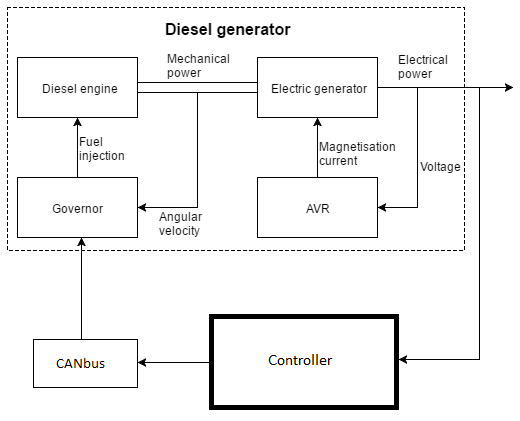
\includegraphics[width=0.6\textwidth]{rapport/billeder/genset_control_approach.png}
\caption{Block diagram illustrating the genset with an addon frequency controller.}
\label{fig:genset_control_approach}
\end{figure}


%This requires the abillity to measure either frequency, Voltage or both on the genset. 
The frequency can be obtained in two ways. Either by making time calculations between zero crossings on one of the three phases of the voltage outputs or by a tachometer. In case of a tachometer, it is required to be installed if it is not already built in the genset. For this reason, voltage measurements are carried out and in the mean time provided to the controller.
When the frequency differs from the reference value after the correction of the governor, in the mean time disturbance will appear in the voltage due to the change in the load, as shown in \figref{fig:4050kwstepvoltage50khz}  

\begin{figure}[H]
\centering
%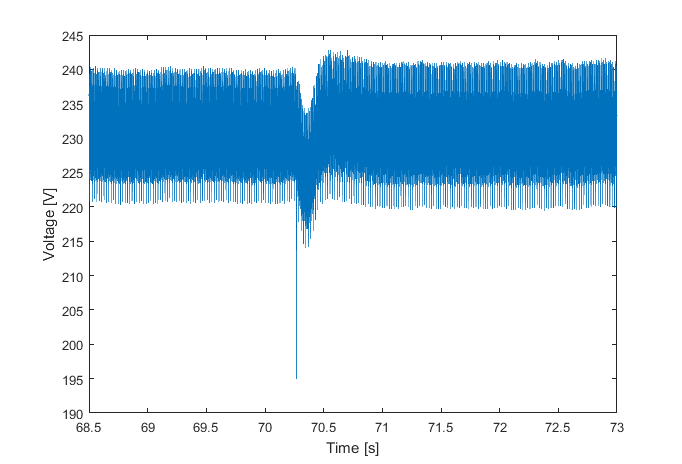
\includegraphics[width=0.8\textwidth]{rapport/billeder/4050kwstep_rmsvoltage50khz.png}
% This file was created by matlab2tikz.
%
%The latest updates can be retrieved from
%  http://www.mathworks.com/matlabcentral/fileexchange/22022-matlab2tikz-matlab2tikz
%where you can also make suggestions and rate matlab2tikz.
%
\definecolor{mycolor1}{rgb}{0.00000,0.44700,0.74100}%
%
\begin{tikzpicture}

\begin{axis}[%
width=4.0in,
height=3.0in,
at={(0.758in,0.481in)},
scale only axis,
xmin=68.5,
xmax=73,
xlabel={Time [s]},
xmajorgrids,
ymin=190,
ymax=245,
ylabel={Voltage [V]},
ymajorgrids,
axis background/.style={fill=white}
]
\addplot [color=mycolor1,solid,forget plot]
  table[row sep=crcr]{%
68.5	236.182596866281\\
68.50234	239.32349979073\\
68.5079	220.8640850444\\
68.51116	223.997851784714\\
68.51574	240.293033346787\\
68.52238	239.77070578819\\
68.52792	220.79004567877\\
68.53118	223.582354444062\\
68.53572	240.125383263619\\
68.54238	239.503125414541\\
68.54794	221.128509605651\\
68.55572	240.384935875427\\
68.56122	223.879546645624\\
68.56794	220.7161680143\\
68.57242	239.441423878054\\
68.57576	240.236675185465\\
68.58122	224.080563660521\\
68.58796	220.893946320023\\
68.5932	239.658824881852\\
68.59578	240.20427038339\\
68.60126	223.727767401031\\
68.60796	220.710497598098\\
68.6132	239.878021302842\\
68.61578	240.17915047505\\
68.62126	223.929956496818\\
68.628	221.053355880053\\
68.63324	239.624493022416\\
68.63578	240.222954057788\\
68.64128	223.684256868545\\
68.64802	220.612101487921\\
68.65326	239.815040382687\\
68.6558	240.142616805618\\
68.66128	223.988394067825\\
68.66802	220.770027168167\\
68.67582	240.112992281759\\
68.6813	223.636064799859\\
68.6825	239.54314601358\\
68.68804	220.53256420538\\
68.69584	239.928065934181\\
68.70132	223.821007005784\\
68.7025	239.372873576282\\
68.70802	221.012353067274\\
68.7158	240.118482472716\\
68.72248	239.010144811714\\
68.728	220.454035978402\\
68.72812	220.769404701112\\
68.73584	239.922309039822\\
68.74248	239.053636110184\\
68.74802	220.496852065587\\
68.7513	223.496990448604\\
68.75582	239.829973192816\\
68.7625	239.303201155633\\
68.768	220.395317294666\\
68.7713	223.209638592102\\
68.7758	239.840855547138\\
68.78248	239.146927793181\\
68.788	220.736257358188\\
68.79128	223.389796772555\\
68.79578	239.885323514174\\
68.80246	238.999895179545\\
68.808	220.536732697186\\
68.81128	223.403391452547\\
68.8158	239.955510850449\\
68.82244	239.140905334421\\
68.828	220.614687436036\\
68.83576	240.058948706701\\
68.84126	223.626190489658\\
68.84244	239.442062625109\\
68.84796	220.495053090767\\
68.85578	239.830749131896\\
68.86126	223.628671248046\\
68.86798	220.835269134597\\
68.8732	239.450790656104\\
68.87576	240.038414243429\\
68.88122	223.542168258213\\
68.88796	220.476301636555\\
68.8932	239.635295053581\\
68.89574	240.147527031996\\
68.90124	224.012113116494\\
68.90796	220.776326643619\\
68.91244	239.56164275001\\
68.91574	240.058522704187\\
68.92122	223.574420286065\\
68.92794	220.617644589382\\
68.93316	239.596264795941\\
68.93572	239.935367816349\\
68.9412	223.697339822694\\
68.94792	220.845221535355\\
68.95572	239.945469608027\\
68.96122	223.468552620758\\
68.96238	238.972112433299\\
68.9679	220.486849924396\\
68.9757	239.899675428779\\
68.9812	223.735482536484\\
68.98236	239.031771772429\\
68.98792	220.495215958117\\
68.99572	239.875814876156\\
69.00236	239.432401189946\\
69.0079	220.558574750186\\
69.00808	221.244478980079\\
69.01572	239.753304743473\\
69.02238	239.1382233014\\
69.0279	220.828234296478\\
69.03116	223.448438077259\\
69.0357	239.957655335617\\
69.04238	238.913665325294\\
69.04792	220.396174890242\\
69.0512	223.232398055629\\
69.05572	239.8939164419\\
69.06238	239.049874067456\\
69.0679	220.557892414327\\
69.0712	223.62162576642\\
69.07574	239.927386259017\\
69.0824	239.367036312264\\
69.08794	220.470729467844\\
69.09118	223.333450948352\\
69.09574	239.881221584246\\
69.10238	239.317570243146\\
69.10792	221.010432681733\\
69.11572	240.271907386541\\
69.12122	223.850365990692\\
69.12794	220.763049114127\\
69.13244	239.484552933483\\
69.13572	240.243263975115\\
69.14122	224.092589100093\\
69.14794	220.900139344682\\
69.15316	239.81050429193\\
69.15572	240.397494072318\\
69.16122	223.916151764077\\
69.16794	220.802030839657\\
69.17318	239.931380598356\\
69.17574	240.273588202074\\
69.1812	224.10823429112\\
69.1879	221.287144010145\\
69.19316	239.894536398289\\
69.19572	240.382391657022\\
69.2012	223.785105486268\\
69.20794	220.721489523562\\
69.21316	239.754234190973\\
69.21572	240.198674495024\\
69.2212	224.068954927942\\
69.22788	220.885839080395\\
69.23572	240.14564721227\\
69.24118	223.671663894126\\
69.24236	239.618019481876\\
69.24792	220.749774089163\\
69.2557	240.021914581079\\
69.26118	223.770787674948\\
69.26234	239.279187091147\\
69.26788	220.916336327239\\
69.27566	240.117647488511\\
69.28234	239.165499380136\\
69.28788	220.648961045405\\
69.28804	221.281776672866\\
69.29568	239.970621682808\\
69.30234	239.16578738224\\
69.30788	220.677288657367\\
69.31114	223.646040211052\\
69.3157	239.990239493366\\
69.32236	239.483270444757\\
69.3279	220.549614245299\\
69.33118	223.413971721593\\
69.3357	239.855190905193\\
69.34236	239.276119046246\\
69.34788	220.949726912971\\
69.35118	223.517968260757\\
69.3557	240.081697032489\\
69.36234	239.017175768814\\
69.3679	220.482076699747\\
69.37116	223.442208225453\\
69.3757	240.03239126036\\
69.38236	239.286402011272\\
69.3879	220.754053025269\\
69.39568	240.038464799568\\
69.40116	223.598768957181\\
69.40234	239.453012309653\\
69.40788	220.567247280544\\
69.41572	239.942101740191\\
69.42118	223.749769320179\\
69.42788	220.951295302456\\
69.43312	239.448412263303\\
69.4357	239.969513471677\\
69.44118	223.529193889374\\
69.4479	220.561111382235\\
69.45316	239.780494237264\\
69.45568	240.246833681008\\
69.46118	224.143983788881\\
69.46792	220.94742245517\\
69.47312	239.870664477929\\
69.47572	240.398044267211\\
69.48118	223.907975656295\\
69.48792	220.839844400869\\
69.49316	239.927122398657\\
69.4957	240.169996760107\\
69.50118	223.954279536955\\
69.5079	221.006992842798\\
69.51572	240.145901506598\\
69.5212	223.628617564367\\
69.52238	239.14481328005\\
69.5279	220.641816285468\\
69.5357	240.074639109903\\
69.54116	223.967422063642\\
69.54236	239.274952874129\\
69.5479	220.753936002094\\
69.55572	240.098271872686\\
69.56236	239.536184309908\\
69.5679	220.628448155302\\
69.56798	220.863565069026\\
69.5757	240.039360596167\\
69.58236	239.364211353919\\
69.5879	220.993195243089\\
69.59116	223.638054631064\\
69.59568	240.202438602144\\
69.60234	239.260804897954\\
69.60788	220.705636350019\\
69.61114	223.612216189471\\
69.61568	240.138132991549\\
69.62234	239.35480212873\\
69.62786	220.852496967244\\
69.63112	223.820778842508\\
69.63568	240.161802446115\\
69.64232	239.610195052124\\
69.64786	220.720251157055\\
69.65112	223.539899845456\\
69.65566	239.978297412842\\
69.66232	239.398434231513\\
69.66786	221.056057417193\\
69.67564	240.195760765221\\
69.68114	223.680614241601\\
69.68786	220.610098882999\\
69.69234	239.314096364485\\
69.69564	240.151616714143\\
69.70112	224.028268886801\\
69.70784	220.823774360726\\
69.71308	239.541137516085\\
69.71568	240.118808049613\\
69.72114	223.672208776966\\
69.72784	220.714751928252\\
69.73308	239.751055350475\\
69.73566	239.951204892092\\
69.74114	223.691141350636\\
69.74786	220.787822590302\\
69.7531	239.320395207972\\
69.75566	239.881836036864\\
69.76114	223.474779291012\\
69.76786	220.440836025225\\
69.77308	239.560570585325\\
69.77564	239.868785528325\\
69.78114	223.754608541925\\
69.78786	220.5549390647\\
69.79564	239.935316912878\\
69.80114	223.529954531639\\
69.80232	239.424322921148\\
69.80784	220.477941191593\\
69.81566	239.725158601818\\
69.82114	223.622601300718\\
69.8223	239.170318714858\\
69.82786	220.873141970114\\
69.83564	239.970333452908\\
69.8423	238.920020940586\\
69.84786	220.464811770873\\
69.84794	220.757055615821\\
69.85566	239.820718736761\\
69.86232	239.08546872231\\
69.86786	220.606670390615\\
69.87112	223.584183204373\\
69.87564	239.824100253707\\
69.88232	239.283034770889\\
69.88786	220.434472618849\\
69.89112	223.273096626269\\
69.89566	239.720548894958\\
69.9023	239.087697582742\\
69.90784	220.737996441294\\
69.91114	223.283891954279\\
69.91564	239.841993994658\\
69.92232	239.031955891885\\
69.92786	220.628471289972\\
69.93112	223.574463150237\\
69.93562	240.03849788888\\
69.94234	239.260377800873\\
69.94788	220.810673640904\\
69.95566	240.122265948343\\
69.96114	223.693600200885\\
69.9623	239.597605154629\\
69.96786	220.625642232304\\
69.97566	239.952371793168\\
69.98114	223.823664433448\\
69.98786	221.01951895798\\
69.99308	239.546435673232\\
69.99566	240.114060352922\\
70.00116	223.637955419394\\
70.00786	220.598125015642\\
70.01312	239.640448337017\\
70.01568	239.942278757656\\
70.02116	223.81270978767\\
70.02788	220.568681433169\\
70.03238	239.374371300306\\
70.03568	239.865177517323\\
70.04114	223.414923917734\\
70.0479	220.447227363111\\
70.05312	239.570279463216\\
70.05568	239.712610701162\\
70.06116	223.524998718451\\
70.0679	220.707248361187\\
70.07566	239.878975236298\\
70.08116	223.430299650883\\
70.08234	238.900911402092\\
70.0879	220.402079188053\\
70.09566	239.821993448613\\
70.10116	223.696765897312\\
70.10234	239.024439780747\\
70.10786	220.51357171952\\
70.1157	239.939284312198\\
70.12232	239.444177884777\\
70.12786	220.495974193219\\
70.1279	220.501600287088\\
70.13566	239.709550267784\\
70.14232	239.173255172027\\
70.14786	220.85842101993\\
70.15112	223.43560721809\\
70.15564	239.871265821204\\
70.16232	238.91849704275\\
70.16786	220.492531288855\\
70.17112	223.39782363346\\
70.17566	240.049168683036\\
70.18232	239.338264043627\\
70.18788	220.912091419679\\
70.19112	223.97443655285\\
70.19566	240.181413857317\\
70.20232	239.740911476153\\
70.20786	220.817069841381\\
70.21114	223.591117239333\\
70.21566	240.104399385281\\
70.2223	239.447194291699\\
70.22784	221.1392080182\\
70.23568	240.27791135995\\
70.24116	223.867110530072\\
70.24788	220.857117272684\\
70.25232	239.406826213247\\
70.25568	240.148974054821\\
70.26116	224.01431664628\\
70.26314	239.06500837464\\
70.26712	194.927871943488\\
70.28118	221.461135604723\\
70.28342	238.225023284184\\
70.28798	217.890902077928\\
70.29674	236.931465455555\\
70.30138	219.715716656395\\
70.30818	216.456559104054\\
70.3135	235.682284040224\\
70.3169	234.837255925957\\
70.32162	217.949096455648\\
70.32844	214.642781490162\\
70.33374	234.370172505839\\
70.3371	233.606686904863\\
70.3419	217.189110305781\\
70.34876	214.076907301052\\
70.35404	233.575589344221\\
70.36226	216.786704648832\\
70.36434	233.656499236415\\
70.36908	214.139446146275\\
70.37444	234.311587199253\\
70.3826	217.62111067748\\
70.38472	234.446375020849\\
70.38948	215.290581250086\\
70.3949	235.509238694402\\
70.40304	218.925521249046\\
70.40518	235.782468270544\\
70.40994	216.455092171756\\
70.41538	237.478499026754\\
70.42354	221.215753587796\\
70.42568	237.650238226615\\
70.43046	218.106409546846\\
70.43588	238.938102710897\\
70.44406	222.672584517792\\
70.4462	239.489918020223\\
70.45098	219.495304382197\\
70.45644	240.740355682562\\
70.4646	223.53553327249\\
70.4667	240.708665649473\\
70.47152	220.709968647582\\
70.477	241.455795967399\\
70.4852	223.727704778413\\
70.4873	240.672548116038\\
70.49214	220.504832004879\\
70.49758	241.853558804186\\
70.5058	225.011297517295\\
70.50786	241.163203514066\\
70.51276	221.015715999451\\
70.51814	242.03481821665\\
70.5264	225.01188973215\\
70.52846	241.727942052114\\
70.53336	221.238318076722\\
70.53876	242.810901860893\\
70.547	224.983763997538\\
70.54902	242.234318915419\\
70.55394	221.831352044746\\
70.55936	242.745016898734\\
70.5676	224.644131071791\\
70.56968	241.655295350285\\
70.57452	221.139226271219\\
70.57994	242.451247354494\\
70.58816	225.189103981705\\
70.5902	241.234672008745\\
70.59512	220.95252754174\\
70.60048	242.18335189996\\
70.60876	225.097410858055\\
70.6108	241.715883709573\\
70.61566	221.027182764549\\
70.62104	242.541741252923\\
70.6313	241.991233807308\\
70.63596	223.117232474507\\
70.6362	221.522941814161\\
70.64158	242.578564378292\\
70.65182	241.333160213739\\
70.6567	220.660717363785\\
70.66208	242.023072677655\\
70.6723	241.070254931006\\
70.67718	220.745603721796\\
70.67744	222.125385715291\\
70.6825	241.980283825804\\
70.69272	241.742250931476\\
70.69758	220.940238667609\\
70.70092	223.687713630335\\
70.70296	242.741588959158\\
70.71312	241.832046035225\\
70.718	221.122892867292\\
70.72132	223.491424262207\\
70.72332	242.133452033687\\
70.73352	241.007664448492\\
70.73836	220.414016682243\\
70.74168	223.862837237075\\
70.74368	241.80145802738\\
70.75386	240.97345073334\\
70.7587	220.579381379093\\
70.762	223.803949385208\\
70.76398	241.857242026848\\
70.77414	241.534165436107\\
70.779	220.487603227672\\
70.7823	223.175786236993\\
70.7843	241.996211876343\\
70.7944	241.214890579956\\
70.79922	220.610673283653\\
70.80252	223.52984164126\\
70.80456	241.705738041287\\
70.81464	240.813513818266\\
70.81944	220.319396582363\\
70.82272	223.537427654744\\
70.82472	241.728050322051\\
70.8348	240.989476127417\\
70.8396	220.336194115946\\
70.84488	241.464953029765\\
70.85298	223.750757680281\\
70.855	241.032439250059\\
70.85976	220.014318662824\\
70.865	241.482662960339\\
70.87308	223.828376519638\\
70.87504	240.863744547618\\
70.87984	220.428231304999\\
70.88512	241.271685661794\\
70.89316	223.606023160715\\
70.89992	219.986612873943\\
70.90514	241.156584677535\\
70.90848	240.765931131774\\
70.91322	223.815660524087\\
70.91994	219.940203758128\\
70.92518	240.994696626468\\
70.93324	223.325270065884\\
70.93528	240.803519708842\\
70.93996	219.737487437662\\
70.94518	241.104001915321\\
70.95322	223.540911733736\\
70.95522	240.620149842894\\
70.95996	220.145299911028\\
70.9652	240.878822729569\\
70.96852	240.377610273572\\
70.97322	223.398490883817\\
70.97992	219.916760531115\\
70.98518	241.035990137711\\
70.9885	240.451658884726\\
70.99318	223.551393816016\\
70.9999	219.854405658609\\
71.0051	240.892893190279\\
71.01516	240.853372255992\\
71.0196	221.682609780665\\
71.01986	219.863155119649\\
71.02506	241.137096314006\\
71.03508	240.55463440852\\
71.03976	220.066053057561\\
71.04304	222.915806929806\\
71.04502	240.753795617362\\
71.05506	240.17966907609\\
71.05968	219.779720567928\\
71.06296	222.993618415789\\
71.06494	240.928542094608\\
71.07498	240.208003396709\\
71.07962	219.750001659082\\
71.08288	223.121081781657\\
71.08486	240.726841327295\\
71.09492	240.774540978346\\
71.0996	219.650510992273\\
71.10282	222.939498752838\\
71.10482	240.914895394446\\
71.1148	240.542884040456\\
71.1195	220.081299490476\\
71.1247	240.879430204892\\
71.13268	223.265548404062\\
71.13478	240.333473402063\\
71.1394	219.742163896122\\
71.14466	240.884146924581\\
71.1526	223.655145862628\\
71.15934	219.915660088324\\
71.16454	240.948286075041\\
71.17254	223.388796673349\\
71.17462	241.110332196003\\
71.17926	220.003414272749\\
71.18448	241.201884342591\\
71.18782	240.730192374852\\
71.19244	223.591763996538\\
71.19918	220.218788580244\\
71.20438	240.82374227586\\
71.20776	240.442013647955\\
71.21236	223.318631201399\\
71.2191	219.917103818878\\
71.22432	241.011798423162\\
71.22762	240.408937303538\\
71.2323	223.321763731729\\
71.23902	219.656006870212\\
71.2442	240.664734922707\\
71.25224	223.254115070324\\
71.2543	240.663246419314\\
71.25896	219.628707282313\\
71.26414	240.900769790004\\
71.27418	240.529293304371\\
71.27882	220.172378844963\\
71.27886	220.150312878307\\
71.28406	240.787448627761\\
71.29408	240.25057871505\\
71.29874	219.891415793303\\
71.30198	223.199870258326\\
71.30398	241.176640508743\\
71.31398	240.672138348176\\
71.31866	220.116628531899\\
71.3219	223.457884967541\\
71.32388	241.138811704828\\
71.33396	241.032922738264\\
71.33858	219.913741138808\\
71.34184	223.316310374246\\
71.34382	241.284111793891\\
71.35384	240.791033518519\\
71.3585	220.304167572926\\
71.36178	223.26353705692\\
71.36374	240.98716997747\\
71.37378	240.459574196821\\
71.37844	219.905116257558\\
71.38366	240.998121210692\\
71.39166	223.576922817778\\
71.39366	240.27168574085\\
71.39838	219.857267145452\\
71.40362	240.823382940348\\
71.4116	223.25735348565\\
71.41832	219.699785455441\\
71.42354	240.952277973081\\
71.43154	223.262546889867\\
71.43354	240.444423693744\\
71.43824	220.092570604772\\
71.44348	240.803027865446\\
71.4469	240.280167417469\\
71.4515	223.190187723012\\
71.45826	219.705236363216\\
71.46348	240.830522835389\\
71.46676	240.426265334094\\
71.47148	223.432522089071\\
71.47818	219.697592940273\\
71.48342	240.667757131936\\
71.49144	223.143497599265\\
71.49354	240.646395260937\\
71.49818	219.717173079014\\
71.5034	241.018651270844\\
71.5114	223.558969313281\\
71.51346	240.633344660502\\
71.51814	220.287016138416\\
71.52336	241.07378970625\\
71.53344	240.4679346694\\
71.53804	220.143184702215\\
71.53812	219.985916571001\\
71.54338	241.111281901981\\
71.5534	240.31949534682\\
71.5581	219.871048737474\\
71.56138	223.285896353569\\
71.56334	240.853008531656\\
71.57338	240.682920409994\\
71.57812	219.652330755333\\
71.58136	222.839099861499\\
71.58336	240.952345089577\\
71.5934	240.467071983532\\
71.5981	220.027562430634\\
71.60134	222.884969631198\\
71.60334	240.712140606611\\
71.6134	239.973707110105\\
71.61814	219.631596016488\\
71.62134	222.96635139448\\
71.62338	240.900395002789\\
71.63338	240.405411384429\\
71.63808	219.988843230363\\
71.64332	241.041957360816\\
71.65136	223.405575341687\\
71.65346	240.93283663883\\
71.6581	219.901444543914\\
71.66338	241.185987837533\\
71.67136	223.518032573251\\
71.67338	240.605905519448\\
71.67812	220.137929655288\\
71.68338	240.897701425488\\
71.69138	223.332074662187\\
71.69812	219.87248079853\\
71.70338	241.005797280722\\
71.70668	240.514771830651\\
71.7114	223.557246932972\\
71.71814	219.819175924592\\
71.72338	240.85835708375\\
71.73142	223.315612908614\\
71.73346	240.740741752582\\
71.7382	219.76003224161\\
71.74342	241.078548100337\\
71.75146	223.380421730509\\
71.7535	240.580479864154\\
71.75822	220.076236435809\\
71.76344	240.916234037718\\
71.7668	240.371300240205\\
71.77148	223.334442550106\\
71.7782	219.809687333915\\
71.78348	241.047061665352\\
71.7869	240.589189759571\\
71.7915	223.710602909578\\
71.79824	219.910641653604\\
71.80346	240.899882925978\\
71.81356	240.819600639324\\
71.818	222.130735364897\\
71.8183	219.782894177224\\
71.82352	241.058687637299\\
71.83356	240.400032714571\\
71.83828	219.986979965103\\
71.84154	222.915638471149\\
71.84354	240.841289588877\\
71.85364	240.241822723307\\
71.85832	219.749919534494\\
71.86156	222.969621085661\\
71.86358	240.867557401019\\
71.87362	240.157044322044\\
71.87832	219.749072097017\\
71.8816	223.158926225609\\
71.88362	240.859032726268\\
71.89368	240.855707690483\\
71.8984	219.734868293018\\
71.90164	222.969973454947\\
71.90362	241.122440694038\\
71.91368	240.614575423539\\
71.9184	220.147759801987\\
71.92168	223.150863930473\\
71.92362	240.916407312786\\
71.93372	240.238323294113\\
71.9384	219.755648984086\\
71.94368	241.141254528164\\
71.95168	223.681289962229\\
71.9537	240.449060895269\\
71.95842	219.865467151696\\
71.96366	240.906237595667\\
71.97172	223.457735097714\\
71.97844	219.801457522844\\
71.98374	241.267308964559\\
71.9839	240.760167447123\\
71.9917	223.559726942078\\
71.99844	220.143235687018\\
72.0037	240.995396308035\\
72.0117	223.5101564853\\
72.01376	240.440943459442\\
72.01848	219.928586657503\\
72.0237	241.237936766622\\
72.027	240.766671497877\\
72.0317	223.757545962142\\
72.03844	220.011860002289\\
72.04368	241.037977103713\\
72.0517	223.457321848043\\
72.05378	240.858528886772\\
72.05846	219.736817603279\\
72.0637	241.113296545075\\
72.07172	223.56000965438\\
72.07376	240.695531005113\\
72.07846	220.188446870894\\
72.0837	240.925129924561\\
72.0917	223.199192030161\\
72.09372	240.142939747178\\
72.09844	219.604930429055\\
72.1037	240.826126009513\\
72.11372	240.160638514447\\
72.11844	219.670019219169\\
72.11868	220.581559698826\\
72.12368	240.658514224513\\
72.13382	240.577299384557\\
72.13844	219.57653242947\\
72.14168	222.82007256884\\
72.1437	240.90479393234\\
72.15376	240.33463801368\\
72.15842	219.906150673797\\
72.1617	222.988760110048\\
72.1637	240.787905786226\\
72.17376	240.216377828581\\
72.17842	219.675859814902\\
72.18168	222.834238420625\\
72.18372	240.865729150427\\
72.19376	240.094480101064\\
72.19842	219.582470626073\\
72.2017	223.079768758098\\
72.20368	240.676196393446\\
72.21378	240.647748816432\\
72.21846	219.579364211439\\
72.22372	240.776943585759\\
72.23172	223.17270930175\\
72.2337	240.319085410419\\
72.23846	219.917944096012\\
72.24372	240.823339253418\\
72.2517	223.230781530945\\
72.25846	219.704429883461\\
72.2637	241.012701623275\\
72.26386	240.739675812727\\
72.27172	223.763743758531\\
72.27846	219.865156829135\\
72.28372	240.976069221614\\
72.29174	223.483267690223\\
72.2938	241.030153391127\\
72.29846	219.885909573958\\
72.30374	241.42409176247\\
72.31174	223.696359724888\\
72.3138	240.814181151671\\
72.31846	220.230969429445\\
72.32372	241.123219170027\\
72.32708	240.519297887404\\
72.33174	223.476321685692\\
72.3385	219.855656482839\\
72.34374	241.031914056521\\
72.34704	240.511023439329\\
72.35176	223.541380746944\\
72.3585	219.676150607737\\
72.36374	240.663461211917\\
72.37174	223.050767530249\\
72.37384	240.473647746311\\
72.37852	219.381537533168\\
72.38374	240.745161880255\\
72.3938	240.333302198912\\
72.39848	219.842655617982\\
72.39864	220.139863212004\\
72.40374	240.695672089259\\
72.41378	240.116844278468\\
72.41846	219.649969767241\\
72.42172	222.966225254335\\
72.42372	240.954638387429\\
72.43376	240.317996469435\\
72.43848	219.772233185102\\
72.4417	223.205969202215\\
72.44372	240.903960592529\\
72.4538	240.947720816501\\
72.45844	219.904977348172\\
72.4617	223.160467535882\\
72.4637	241.270827360907\\
72.47374	240.644237218035\\
72.47842	220.11225379527\\
72.48168	223.10763237729\\
72.4837	241.009167464815\\
72.49376	240.576144174424\\
72.49842	220.067890448039\\
72.50366	241.333317434967\\
72.51166	223.908378886134\\
72.51374	240.654329922436\\
72.51838	220.132611783973\\
72.52364	241.331075970681\\
72.53166	223.688345439401\\
72.53838	220.068069606694\\
72.54366	241.44457751297\\
72.5438	241.165146886769\\
72.55166	223.821430869939\\
72.55836	220.483357034418\\
72.5636	241.209766722867\\
72.56698	240.566744463292\\
72.57162	223.391134350157\\
72.57838	219.822211068779\\
72.58362	240.903119034222\\
72.58696	240.462609381202\\
72.59162	223.486658578314\\
72.59838	219.641855025782\\
72.60362	240.652319877661\\
72.61166	223.10756911372\\
72.61372	240.632668059638\\
72.61836	219.612692336797\\
72.62366	240.846383549245\\
72.62698	240.254519229955\\
72.63164	223.190577781448\\
72.63838	219.787265279785\\
72.64366	240.480247153136\\
72.65164	223.022179623836\\
72.65372	239.957823116897\\
72.6584	219.568247030773\\
72.66368	240.848576002641\\
72.67374	240.109430238763\\
72.67842	219.639964511053\\
72.6786	220.07571306068\\
72.68368	240.781234669046\\
72.69376	240.807657620662\\
72.69844	219.780550232309\\
72.7017	223.06971082022\\
72.70372	241.187771767144\\
72.71374	240.762498161224\\
72.71846	220.231871770981\\
72.7217	223.17577433494\\
72.72372	241.095722475189\\
72.7338	240.448070233817\\
72.73848	219.901494755796\\
72.74172	223.164203372016\\
72.74376	241.153129407264\\
72.75376	240.45436590616\\
72.75848	219.930660119085\\
72.76176	223.366459219299\\
72.76378	241.104988045492\\
72.77382	241.00173949061\\
72.77852	219.905638617643\\
72.78378	241.33820073792\\
72.7918	223.775075992427\\
72.79382	240.794538650174\\
72.79854	220.268062421488\\
72.8038	241.262817448801\\
72.8118	223.71783404734\\
72.81854	220.132207671133\\
72.82376	241.275583056319\\
72.8238	241.322688747177\\
72.83184	223.990393209173\\
72.83856	220.067937190238\\
72.8438	241.331084927084\\
72.85182	223.701926283429\\
72.85386	241.203699140719\\
72.85858	220.070682892452\\
72.86382	241.615139478055\\
72.87186	223.945243144576\\
72.87386	241.020461938228\\
72.87856	220.433193417908\\
72.88382	241.36807322186\\
72.88722	240.80811236162\\
72.89184	223.788123148884\\
72.8986	220.217125928215\\
72.90382	241.572033986069\\
72.90714	241.03052635593\\
72.91186	224.038828247471\\
72.91858	220.163823237379\\
72.92386	241.233233765409\\
72.93186	223.7169557769\\
72.93392	241.039440172661\\
72.93862	219.958775138472\\
72.94386	241.357815070972\\
72.95388	240.669066311329\\
72.95856	220.227930813548\\
72.95862	220.113528235999\\
72.96386	241.001194455892\\
72.97396	240.308542663559\\
72.97864	219.83946853803\\
72.98192	223.185838111053\\
72.98388	241.193582673579\\
73.00002	233.173772936445\\
};
\end{axis}
\end{tikzpicture}% 
\caption{Voltage measured on all three phases with Hioki oscilloscope at 50 kHz sampling rate with RMS calculated, before and after a power step from 40 to 50 kW is performed on a genset located at DEIF.}
\label{fig:4050kwstepvoltage50khz}
\end{figure}

The first issue that arises is the noise in the measurement shown in \figref{fig:4050kwstepvoltage50khz}. Because of this, some difficulties appear concerning the design of the controller when the output voltage of the genset fluctuates between 220 to 240 volts in a steady-state mode. The solution which has been provided by Jesper Viese Knudsen, in the simulink blocks is described in \secref{dspace_unitv2}. The dSPACE unit samples the output voltage of the genset at 1 kHz, where sixteen samples are then averaged giving a 62.5 Hz input rate to the controller. The output of this sampling operation is shown in \figref{fig:4050kwstepvoltage62.5hz}. 

\begin{figure}[H]
\centering
% This file was created by matlab2tikz.
%
%The latest updates can be retrieved from
%  http://www.mathworks.com/matlabcentral/fileexchange/22022-matlab2tikz-matlab2tikz
%where you can also make suggestions and rate matlab2tikz.
%
\definecolor{mycolor1}{rgb}{0.00000,0.44700,0.74100}%
%
\begin{tikzpicture}

\begin{axis}[%
width=3.521in,
height=2.566in,
at={(0.758in,0.481in)},
scale only axis,
xmin=68.5,
xmax=73,
xlabel={Time [s]},
ymin=224,
ymax=236,
ylabel={Voltage [V]},
axis background/.style={fill=white}
]
\addplot [color=mycolor1,solid,forget plot]
  table[row sep=crcr]{%
68.496	232.251449569516\\
68.512	232.116248346484\\
68.528	233.64890076305\\
68.544	232.817435120229\\
68.56	232.269923036835\\
68.576	232.180268285985\\
68.592	232.232821803907\\
68.608	233.511499938504\\
68.624	232.664112503649\\
68.64	232.147245877425\\
68.656	232.000145361167\\
68.672	232.171771917135\\
68.688	233.359675912275\\
68.704	232.410735494188\\
68.72	232.094375321851\\
68.736	231.802547979314\\
68.752	231.899619719769\\
68.768	233.118656570701\\
68.784	232.291522758853\\
68.8	231.848666635778\\
68.816	231.866028285432\\
68.832	232.016802515841\\
68.848	233.329475099936\\
68.864	232.392386586747\\
68.88	231.963488845695\\
68.896	231.976358088346\\
68.912	232.088525089789\\
68.928	233.413210070936\\
68.944	232.569831812258\\
68.96	231.933734500629\\
68.976	231.942595585816\\
68.992	231.799574919604\\
69.008	233.275509754118\\
69.024	232.499853539223\\
69.04	231.94214887262\\
69.056	231.862138744768\\
69.072	231.853501090939\\
69.088	233.264494621304\\
69.104	232.553738631634\\
69.12	232.170578126516\\
69.136	232.24798440205\\
69.152	232.20806953032\\
69.168	233.70888655265\\
69.184	232.90285536249\\
69.2	232.397924917593\\
69.216	232.229201069961\\
69.232	232.141022686801\\
69.248	233.516567463417\\
69.264	232.769304097647\\
69.28	232.087818340009\\
69.296	232.154646498921\\
69.312	231.916663566561\\
69.328	233.404419681412\\
69.344	232.646428285034\\
69.36	232.070278841888\\
69.376	232.050233959554\\
69.392	232.008302098164\\
69.408	233.43973945943\\
69.424	232.634988087114\\
69.44	231.994070162002\\
69.456	232.118936247902\\
69.472	232.20973380642\\
69.488	233.764682120991\\
69.504	232.860295957641\\
69.52	232.141863935973\\
69.536	232.123827410259\\
69.552	232.030012072503\\
69.568	233.472663027735\\
69.584	232.787180540395\\
69.6	232.177124658009\\
69.616	232.261945125468\\
69.632	232.067984058275\\
69.648	233.580190321213\\
69.664	232.819259631877\\
69.68	232.239860434024\\
69.696	232.22736497349\\
69.712	232.091790564866\\
69.728	233.551880467081\\
69.744	232.758637754491\\
69.76	231.93658601535\\
69.776	232.007048897476\\
69.792	231.807541762637\\
69.808	233.352695966716\\
69.824	232.598915306936\\
69.84	232.040229644767\\
69.856	232.03147678331\\
69.872	231.814185187302\\
69.888	233.300024060635\\
69.904	232.563580181608\\
69.92	231.898440435307\\
69.936	232.187284998009\\
69.952	232.010504938726\\
69.968	233.550046886092\\
69.984	232.783378340032\\
70	232.169669817287\\
70.016	232.124472085576\\
70.032	231.862007222445\\
70.048	233.26619785203\\
70.064	232.502576213765\\
70.08	231.864389729332\\
70.096	231.933040748994\\
70.112	231.786971098717\\
70.128	233.388067890249\\
70.144	232.550971832024\\
70.16	231.971586256247\\
70.176	232.060278230971\\
70.192	232.098281647715\\
70.208	233.686849406811\\
70.224	232.939266674927\\
70.24	232.319253722182\\
70.256	232.363732118338\\
70.272	231.052725758443\\
70.288	231.328372653101\\
70.304	229.259754431011\\
70.32	227.784751038288\\
70.336	226.28486478479\\
70.352	226.356925362287\\
70.368	226.548439476999\\
70.384	225.864120663848\\
70.4	227.838874901422\\
70.416	228.122665437129\\
70.432	230.070294983649\\
70.448	232.279262348935\\
70.464	232.226236569789\\
70.48	232.562977263779\\
70.496	232.885104290305\\
70.512	234.912915461568\\
70.528	233.544008456963\\
70.544	234.302942230274\\
70.56	233.703073145207\\
70.576	233.956716467103\\
70.592	235.166499678207\\
70.608	233.828417969806\\
70.624	233.366437457811\\
70.64	233.748508481273\\
70.656	234.946354235433\\
70.672	233.5268004611\\
70.688	233.747655753545\\
70.704	233.650766154695\\
70.72	233.622130187609\\
70.736	234.14438942169\\
70.752	233.870781993417\\
70.768	233.443261203925\\
70.784	232.677160149025\\
70.8	233.834080616808\\
70.816	234.115885368237\\
70.832	233.109467044221\\
70.848	232.943595982628\\
70.864	232.378351183493\\
70.88	234.426809765027\\
70.896	233.330237546494\\
70.912	232.517375705827\\
70.928	232.433277201844\\
70.944	232.3053151428\\
70.96	233.985676469822\\
70.976	232.964033086596\\
70.992	232.328266747979\\
71.008	232.488591082381\\
71.024	232.237561173124\\
71.04	234.035578605595\\
71.056	233.006245118356\\
71.072	232.427967448264\\
71.088	232.411480576861\\
71.104	231.906205229016\\
71.12	233.691926419567\\
71.136	233.112715297968\\
71.152	232.420259178693\\
71.168	232.232833683056\\
71.184	232.213168363914\\
71.2	233.242117637983\\
71.216	233.413050973459\\
71.232	232.509843510641\\
71.248	232.103730175736\\
71.264	232.011593800413\\
71.28	232.873862407389\\
71.296	233.502280397913\\
71.312	233.101713809533\\
71.328	233.058715721681\\
71.344	232.185665093918\\
71.36	233.22179504934\\
71.376	233.183000508726\\
71.392	232.914980327856\\
71.408	232.768699022011\\
71.424	231.726194981156\\
71.44	232.623351243245\\
71.456	232.987747188635\\
71.472	232.550065998251\\
71.488	232.681556650507\\
71.504	231.765494360563\\
71.52	232.677137991314\\
71.536	233.344497956787\\
71.552	232.643590974936\\
71.568	232.976084471671\\
71.584	231.874407393658\\
71.6	232.397359717993\\
71.616	233.012505402917\\
71.632	232.469702165938\\
71.648	233.097730288341\\
71.664	232.086962718047\\
71.68	232.625717125542\\
71.696	233.225032909238\\
71.712	232.578377118452\\
71.728	232.931694318347\\
71.744	231.847870528491\\
71.76	232.588338461857\\
71.776	233.118576258087\\
71.792	232.776260080183\\
71.808	232.932596138131\\
71.824	231.850483809871\\
71.84	232.65430737604\\
71.856	232.964789271316\\
71.872	232.739939985592\\
71.888	232.727760396281\\
71.904	231.75899709317\\
71.92	232.900313494637\\
71.936	233.038003425124\\
71.952	232.953202651324\\
71.968	232.874070514084\\
71.984	231.85242909856\\
72	233.052528618872\\
72.016	233.199121197142\\
72.032	233.107627966594\\
72.048	232.989878579292\\
72.064	231.820997509231\\
72.08	232.99723764434\\
72.096	232.995013422302\\
72.112	232.731066394715\\
72.128	232.633071590528\\
72.144	231.560343716782\\
72.16	232.719514450675\\
72.176	232.954539851237\\
72.192	232.752864719806\\
72.208	232.634234996637\\
72.224	231.594253165812\\
72.24	232.616317893772\\
72.256	232.975630187318\\
72.272	232.978289128635\\
72.288	232.88340515495\\
72.304	231.972709539727\\
72.32	233.194203914211\\
72.336	233.278846366929\\
72.352	232.962757833268\\
72.368	232.650919924308\\
72.384	231.461561312247\\
72.4	232.693479050195\\
72.416	232.900231376653\\
72.432	232.876422128318\\
72.448	232.814832033489\\
72.464	231.923086283298\\
72.48	233.017461069544\\
72.496	233.226768742946\\
72.512	233.221343835813\\
72.528	233.154851966656\\
72.544	232.161370876316\\
72.56	233.242218288926\\
72.576	233.241088227942\\
72.592	232.782551987061\\
72.608	232.566069261898\\
72.624	231.557426985776\\
72.64	232.586667693532\\
72.656	232.690875521801\\
72.672	232.64557919328\\
72.688	232.669782435138\\
72.704	231.82799858649\\
72.72	233.079562012931\\
72.736	233.226746078392\\
72.752	233.102793936766\\
72.768	232.998336719037\\
72.784	232.019594405408\\
72.8	233.256925367217\\
72.816	233.562277673375\\
72.832	233.364482335795\\
72.848	233.171413821331\\
72.864	232.257525154906\\
72.88	233.471039555012\\
72.896	233.745193150055\\
72.912	233.520829146605\\
72.928	233.250933793244\\
72.944	232.187633628563\\
72.96	233.120881047595\\
72.976	233.476532248812\\
72.992	233.191304074376\\
73.008	233.079589031756\\
};
\end{axis}
\end{tikzpicture}% 
\caption{Voltage measured on all three phases with Hioki oscilloscope at 50 kHz sampling rate and RMS calculated, before and after a power step from 40 to 50 kW is performed on a genset located at DEIF. Data is then down sampled to 1 kHz and 16 samples is averaged to get a 62.5 Hz output.}
\label{fig:4050kwstepvoltage62.5hz}
\end{figure}

The 62.5 Hz sampling rate and the reduction in fluctuation shown between \figref{fig:4050kwstepvoltage50khz} and \figref{fig:4050kwstepvoltage62.5hz} is considered acceptable on the grounds, that the update interval to the governor is 25 Hz and an apparent change in Voltage is registered in the 1 kHz averaged 62.5 Hz measuring, when a change in load occurs. 
In order to be able to design a controller, modeling of the genset and inverter is needed. Along with the dynamics describing how changes in load affects voltage on the genset, the effects of frequency reference changes on the voltage output are also required. A block diagram, giving an overview of what needs to be modeled is shown in \figref{fig:gensetmodeling}.



\begin{figure}[H]
\centering
\begin{tikzpicture}
 \definecolor{mycolor1}{rgb}{0.00000,0.44700,0.74100} 
\draw  [fill=mycolor1!20](-5.5,2.5) rectangle (-1.5,1.5);
\draw [fill=mycolor1!20] (-2,4.5) rectangle (1.2,3.2);
\node at (-0.5,4.2) {\normalsize{Genset}};
\node at (-0.5,3.8) {\normalsize{\footnotesize{(Change in load to}}};
\node at (-0.5,3.5) {\normalsize{\footnotesize{voltage disturbance)}}};
\node at (-3.5,2.2) {\normalsize{Genset}};
\node at (-3.5,1.8) {\normalsize{\footnotesize{(Frequency to voltage)}}};

\draw [fill=mycolor1!20] (-5,6) rectangle (-2,5);
\draw [-latex] (-0.4,2) ellipse (0.25 and 0.25);
\draw [-latex](-1.5,2) -- (-0.6,2);
\draw [-latex](-0.4,3.2) -- (-0.4,2.2);
\draw [-latex] (-9.5,2.5) rectangle (-7.5,1.5);
\node at (-8.5,2) {Controller};
\draw [-latex](-7.5,2) -- (-5.5,2);

\node at (-0.2,2.4) {$+$};
\draw [-latex] (-10.9,2) ellipse (0.25 and 0.25);
\draw [-latex](-10.64,2) -- (-9.5,2);


\draw [-latex](-13,2) -- (-11.1,2);
\node at (-12.5,2.5) {\normalsize{\footnotesize{Voltage error}}};
\node at (-12.78,2.25) {\normalsize{\footnotesize{reference}}};
\draw [-latex](-0.17,2) -- (3,2);

\draw [-latex](0.6,2) -- (0.6,0.6) -- (-10.9,0.6) -- (-10.9,1.77);
\node at (-10.7,1.6) {$-$};
\node at (-11.3,2.3) {$+$};
\node at (-0.8,2.3) {$+$};
\node at (2,2.25) {\normalsize{\footnotesize{Genset voltage output}}};
\node at (-6.5,2.2) {\footnotesize{Frequency}};
\draw [-latex](2,5.5) -- (-0.25,5.5);
\node at (1.2,5.8) {\normalsize{\footnotesize{Resistive load}}};
\draw [-latex] (-0.5,5.5) ellipse (0.25 and 0.25);


\node at (-3.5,5.75) {\normalsize{Inverter}};
\node at (-3.5,5.4) {\normalsize{\footnotesize{(Power dynamics)}}};

\draw [-latex](2,5.5) -- (-0.25,5.5);
\draw [-latex](-2,5.5) -- (-0.75,5.5);
\draw [-latex](-0.5,5.25) -- (-0.5,4.5);
\draw [-latex](-7,5.5) -- (-5,5.5);

\node at (-6.5,5.8) {\normalsize{\footnotesize{Resistive load}}};
\node at (0.5,5) {\normalsize{\footnotesize{Power(W)}}};
\node at (0.5,2.75) {\normalsize{\footnotesize{Voltage(V)}}};

\node at (0,5.8) {$+$};
\node at (-1,5.8) {$-$};
\end{tikzpicture} 
%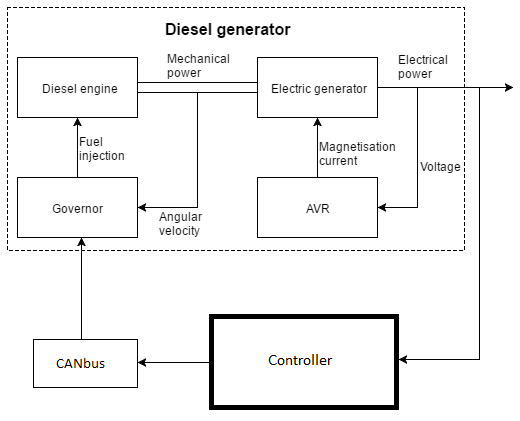
\includegraphics[width=0.6\textwidth]{rapport/billeder/genset_control_approach.png}
\caption{Block diagram showing combined inverter and genset with controller, where blocks in lightblue indicates systems to be modeled.}
\label{fig:gensetmodeling}
\end{figure}


%\begin{figure}[H]
%\centering
%\includegraphics[width=1\textwidth]{rapport/billeder/gensetmodeling.png}
%\caption{Block diagram showing combined inverter and genset with controller, where blocks in lightblue indicates systems to be modeled.}
%\label{fig:gensetmodeling}
%\end{figure}

For the sake of comparison between the simulation and measurements, genset systems for frequency to power and power to power models is added to the list of models to be derived. The derivation of the various models is to be described in the section to come. 



%The Voltage reference is given to the AVR as an RMS value of all three phases, which mean it needs to be calculated before it can be used by a controller. 


%On \figref{fig:4050kwstepfreq} and \figref{fig:4050kwstepvoltage50khz} frequency and Voltage is shown during a 40 to 50 kW step in load. 

% The RMS Voltage can be calculated by the following equation:

% \begin{equation} 
% \label{eq:Vrms}
% V_{RMS} = \sqrt{\frac{V_{1}^2+V_{2}^2+V_{3}^2}{3}}
% \end{equation}

% Where $V_1$, $V_2$ and $V_3$ is the individual phases.







%Due to the amount of noise at the output of the genset it will be difficult to control by  





%To correct the disturbance appearing when a change in load occurs as shown on \figref{fig:steps_model_comparison} a measurement on the output of the genset is necessary. This could be Voltage, current and electrical frequency, where Voltage and current could be used to calculate power output of the genset. The only known references given to the genset is frequency and Voltage

%\begin{figure}[H]
%\centering
%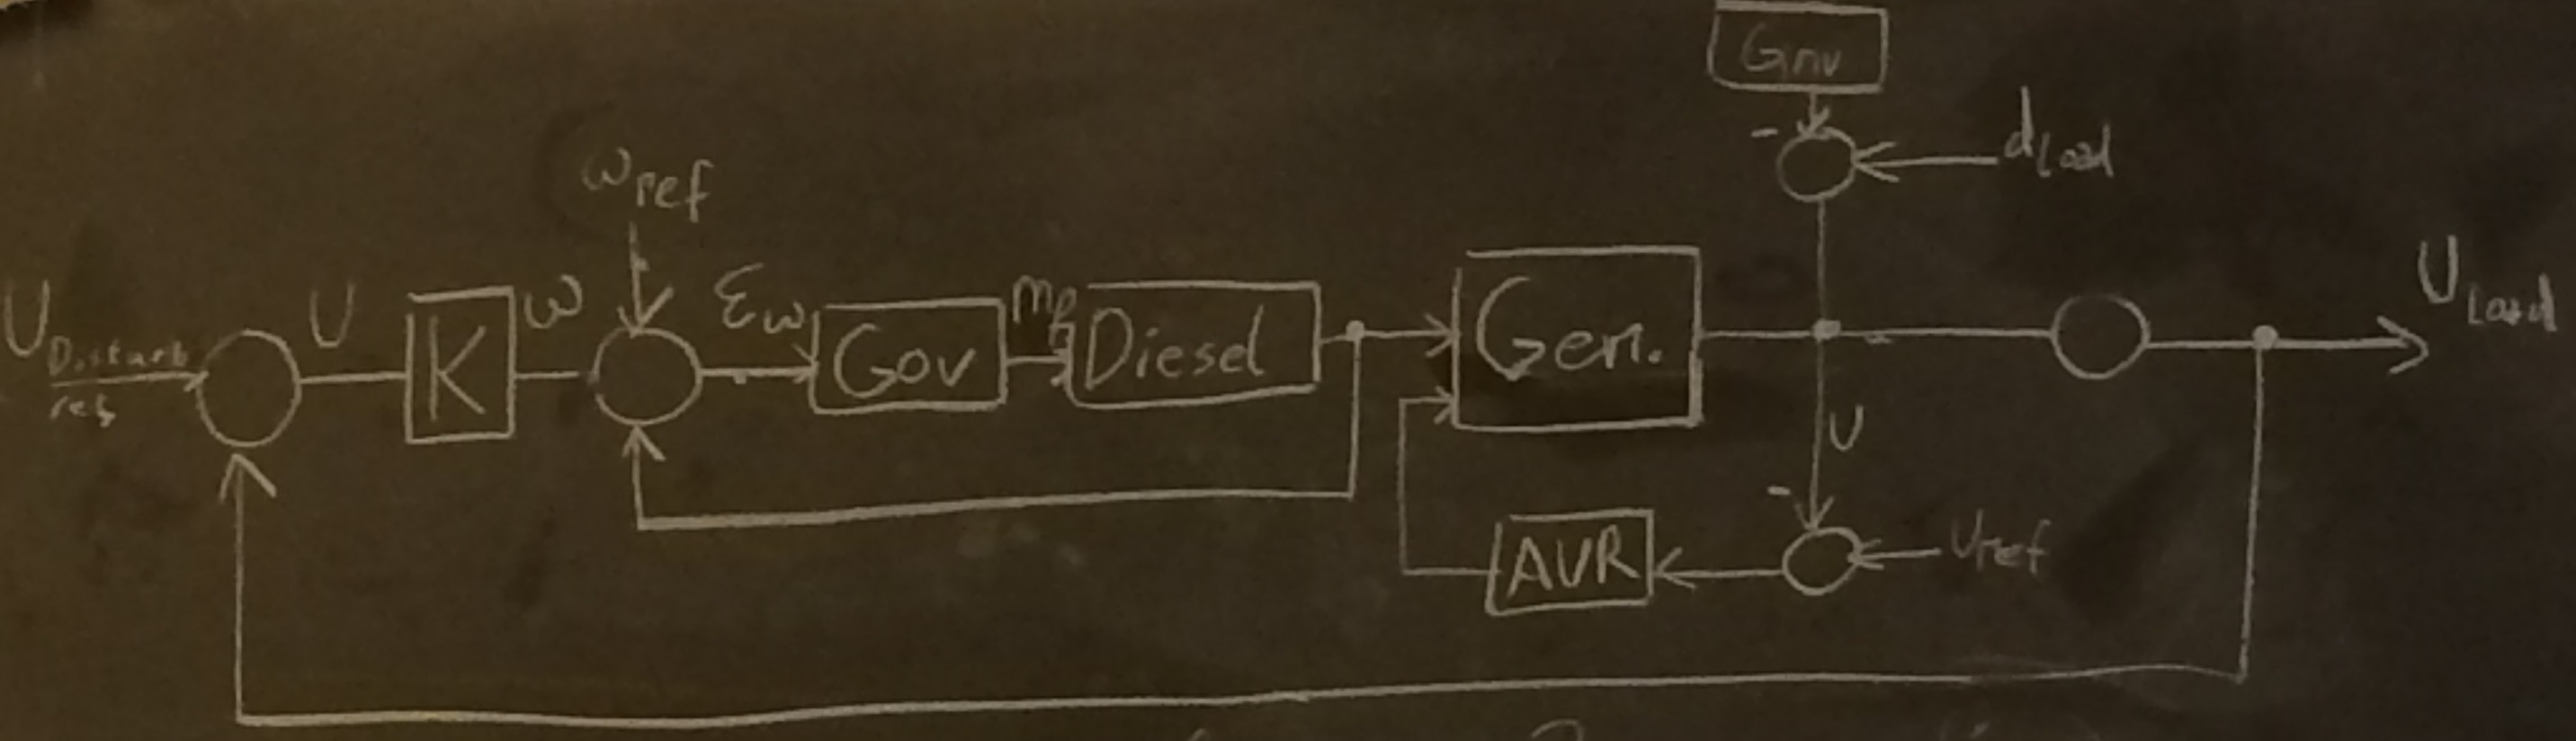
\includegraphics[width=0.75\textwidth]{rapport/billeder/blok}
%\caption{.}
%\label{fig:blok}
%\end{figure}



\chapter{Modeling}
% \section{Grid-connected PV inverter}
% \label{PVinverter}

% During the application of PV inverters the main task is to convert PV power provided by the solar panels in DC voltage to AC, stabilize the output voltage, frequency and current, and feed power to the utility grid. When the inverter works parallel to the genset, the main task is to deliver power according to the reference provided by the ASC. Furthermore the power should be delivered at the voltage and frequency provided by the genset, the inverter should therefore always match this.
% A typical diagram of a grid connected PV system can be seen in \figref{fig:gridPV}.    
% \begin{figure}[H]
% \begin{tikzpicture}
%     \coordinate (SolarCellP) at (0.5,0);
%     \coordinate (ChopperP) at (4,0);
%     \coordinate (InverterP) at (8,0);

%     % Place blocks
%     \begin{scope}[every node/.style={draw,thick, fill=white!30, rectangle,text width=1.5cm, minimum height=2cm, text badly centered}]
%         \node[name=pv,pattern=grid,pattern color=white!30] at (SolarCellP) { PV};
%         \node[name=chopper] at (ChopperP) {DC/DC};
%         \node[name=inverter] at (InverterP) {DC/AC};
%     \end{scope}

%     \draw
%     % PV to chopper
%         (pv.30) -- (chopper.150)
%         (pv.330) -- (chopper.210)
%     % DC link and cap
%         (chopper.30) -- (inverter.150)
%         (chopper.330) -- (inverter.210)
%         ($(chopper.330)!0.4!(inverter.210)$) to[capacitor, l=\SI{}{}, mirror] ($(chopper.30)!0.4!(inverter.150)$)
%     % AC side
%         (inverter.30)
%         to[L] ++(1.1,0)
%         %to[short] ++(1,0)
%         to[L] ++(1.1,0)
%         to[short] ++(1,0) coordinate(N1)
%         to[short] ++(1,0)  %line
%         |- (inverter.330)
%         % ------------------------ Secondary side
%         (N1)++(0.65,0) coordinate (N2)
%             %to[open] ($(N2)+(0,-1)$)
%             %to[short] (N2)
%             %to[short] ++(1,0)
%             to[sV, l=$Grid$] ++(0,-1)
%             %to[short] ++(-1,0)
%     ;
%     \draw ($(inverter.330)+(1.1,0)$) to[C] ++(0,1.033);
%     \draw[thick,dashed] ($(-1.5,-1.5)+(chopper)$) -- ($(-1.5,2)+(chopper)$) -- ($(3.1,2)+(inverter)$) -- ($(3.1,-1.5)+(inverter)$) -- ($(-1.5,-1.5)+(chopper)$);
%     \node[] at ($(2.5,1.5)+(chopper)$) {\textbf{Inverter}};
% \end{tikzpicture}
% \caption{Grid-connected PV system.}
% \label{fig:gridPV}
% \end{figure}

% As can be seen in \figref{fig:gridPV} the system usually consists of a boost (DC/DC) converter which scales up the output voltage of the PV to a certain DC level. According to the available power, usually an algorithm called MPPT (Maximum Power Point Tracker) controls the output current and voltage in such a way that the output power is the maximum possible. The DC/AC inverter provides a 3-phase (or in some cases 1-phase) voltage and current signals, therefore the energy from a solar cell can be utilized and transported to the utility grid. 

% In order to create sinusoidal voltage on the output, usually LC or LCL filters are applied that dampen the high frequency peaks and leaving only the lower frequencies in the inverter output. 
% \section{General inverter concepts}
% \label{inverter}

% In the presented project an inverter from SMA with model number STP20000 of the Pulse Width Modulation(PWM)-type was provided. This kind of unit is capable of creating both active- and reactive-power from 3-phase voltages and currents in accordance with the load on the system. Although the control for such electronic devices can vary in a wide range, there are existing several schemes to generate AC voltage from DC via PWM. Out of several techniques, a scheme called sinusoidal pulse width modulation (SPWM) is assumed and will be discussed, as the outcome of applying other schemes will be somewhat similar and the SPWM scheme provides a basic understanding of the working principle.

% Despite the fact that the project deals with a 3-phase inverter, it is sufficient to introduce the basic concepts of operation in a 1-phase example.
% A basic hardware structure allowing for PWM control is a H-bridge as seen on \figref{fig:inverterblock}, more advanced and sophisticated structures are most likely used in the provided inverter as these improve both efficiency, noise canceling and leakage currents, but the working principle is somewhat the same \cite{aau_invert_topologies}. 


% \begin{figure}[H]
% \centering
% \begin{circuitikz}[thin,scale=1, every node/.style={scale=0.78}]

% % TRANSISTORS
% \draw
% (0,2) node[nigfete] (t1) {}
% (0,0) node[nigfete] (t2) {}
% (2,2) node[nigfete] (t3) {}
% (2,0) node[nigfete] (t4) {};
% \draw
% (t1.S) to[short] (t2.D)
% (t3.S) to[short] (t4.D);
% % DIODES and transistor labels
% \foreach \num in {1,2,3,4} {
% \node[anchor=south] at (t\num.G) {$T_\num$};
% \draw (t\num.S)++(0,0.5) -- ++(0.3,0) to[sD*] ($(t\num.D)+(0.3,-0.5)$) -- ++(-0.3,0);
% }          
% % BATTERY connection
% \draw
% (t4.S) to[short,-*] (t2.S) to[short] ($(t2.S)+(-2,0)$)
% to[battery,l=$U$] ($(t1.D)+(-2,0)$) to[short,-*] (t1.D) to[short] (t3.D);
% % RL
% \draw
% (t1.S) to[short,*-] ($(t1.S)+(3,0)$) to[short] ($(t1.D)+(3,0)$) coordinate (p1)
% to[R,l_=$R$] ++(2,0) to[L,l_=$L$,i>^=$i_L$] ++(3,0) coordinate (p);
% \draw
% (t4.D) to[short,*-] ($(t4.D)+(1,0)$) to[short] ($(t4.S)+(1,0)$) coordinate (n1)
% to[short] ++(5,0) coordinate (n);
% % C
% \draw
% (p) to[C,l=$C$,i>^=$i_C$,v<=$U_C$] (n);
% % LOAD
% \draw
% (p) to[short,*-]($(p)+(2,0)$) to[R,l=$LOAD$,i>^=$i_o$] ($(n)+(2,0)$) to[short,-*] (n);
% % U_i
% \draw
% (p1) to[open,v^=$U_i$] (n1);

% \end{circuitikz}
% \caption{Full-bridge inverter with load}
% \label{fig:inverterblock} 
% \end{figure}

% Most of the inverters usually deal with a full-bridge topology consisting of MOSFETs or IGBTs. The 1-phase circuit illustrated in \figref{fig:inverterblock} has four semiconductor switches with protection diodes, making it possible to create both current and voltage signals with controllable magnitude and frequency, thus controllable active and reactive power components. Each of these switches are controlled by the modulated control signal, namely $T_1$ and $T_4$ with $S$ while $T_2$ and $T_3$ with  $\neg{S}$ which is the negated signal of $S$.

% The scheme of modulating $S$ can be seen in \figref{fig:sinPWM} where a sine (control signal - $V_{control}$) and a triangular (reference signal - $V_{tri}$) are compared.   

% \begin{figure}[H]
% \centering
% 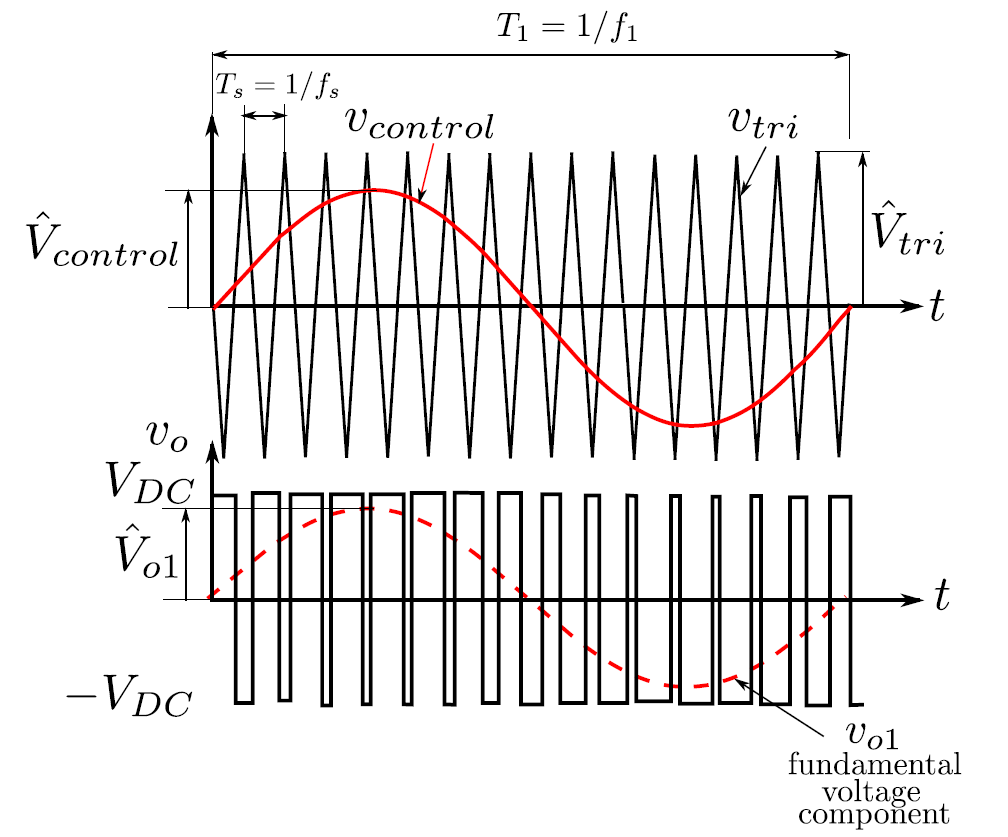
\includegraphics[width=0.6\textwidth]{rapport/analyse/sinPWM}
% \caption{Sinusoidal PWM \cite{bud_inverter_PV}}
% \label{fig:sinPWM}
% \end{figure}

% As can be seen, there are two cases given. When 
% \begin{equation} 
% \label{eq:case1}
% V_{control} > V_{tri} %\unit{W}
% \end{equation}
% then $T_1$ and $T_4$ are conducting, thus switching the DC voltage coming from the PV, while $T_2$ and $T_3$ are turned off. However, when 
% \begin{equation} 
% \label{eq:case1}
% V_{control} < V_{tri}
% \end{equation}
% then $T_2$ and $T_3$ are conducting and switching $V_{DC}$ therefore $T_1$ and $T_4$ are turned off. As can be seen, this switching pattern results in a PWM output signal with a sinusoidally varying duty cycle. While the output voltage is a square signal, the output current can result in an almost perfectly sinus wave(according to the load on the system) if the switching frequency is sufficiently high. Thus, as mentioned previously usually an LC or LCL filter is applied to the inverter voltage output in order to dampen the high frequency components. 

% The frequency of the desired output voltage can be determined by the frequency of the control signal $f_1$ which is the fundamental component of the waveform. The switching frequency equals to the frequency of $V_{tri}$, while the magnitude of the triangular waveform is usually kept constant in order to simplify the control of the voltage and frequency. Therefore the two modulation indexes can be given as: 
% \begin{equation} 
% \label{eq:ma}
% m_a = \frac{\tilde{V}_{control}}{\tilde{V}_{tri}}
% \end{equation}
% \begin{equation} 
% \label{eq:mf}
% m_f = \frac{f_1}{f_s}
% \end{equation}

% where $\tilde{V}_{control}$ and $\tilde{V}_{tri}$ are magnitudes of the signals.

% As can be seen from the relations, the controller of the inverter should measure frequency and voltage of the output waveforms at the same time to modify $m_a$ and to align the desired frequency by adjusting $m_f$.







% This file was created by matlab2tikz.
%
%The latest updates can be retrieved from
%  http://www.mathworks.com/matlabcentral/fileexchange/22022-matlab2tikz-matlab2tikz
%where you can also make suggestions and rate matlab2tikz.
%
\definecolor{mycolor1}{rgb}{0.00000,0.44700,0.74100}%
%
\begin{tikzpicture}

\begin{axis}[%
width=4.396in,
height=3.357in,
at={(0.883in,0.481in)},
scale only axis,
separate axis lines,
every outer x axis line/.append style={white!40!black},
every x tick label/.append style={font=\color{white!40!black}},
xmin=0,
xmax=40,
xmajorgrids,
every outer y axis line/.append style={white!40!black},
every y tick label/.append style={font=\color{white!40!black}},
ymin=0,
ymax=12000,
ymajorgrids,
axis background/.style={fill=white}
]
\addplot [color=mycolor1,solid,forget plot]
  table[row sep=crcr]{%
0	0\\
0.127620402539762	0\\
0.255240805079523	0\\
0.382861207619285	0\\
0.510481610159046	0\\
0.638102012698808	0\\
0.765722415238569	0\\
0.893342817778331	0\\
1.02096322031809	0\\
1.14858362285785	0\\
1.27620402539762	0\\
1.40382442793738	0\\
1.53144483047714	0\\
1.6590652330169	0\\
1.78668563555666	0\\
1.91430603809642	0\\
2.04192644063618	0\\
2.16954684317595	0\\
2.29716724571571	0\\
2.42478764825547	0\\
2.55240805079523	0\\
2.68002845333499	0\\
2.80764885587475	0\\
2.93526925841451	0\\
3.06288966095428	0\\
3.19051006349404	0\\
3.3181304660338	0\\
3.44575086857356	0\\
3.57337127111332	0\\
3.70099167365308	0\\
3.82861207619285	0\\
3.95623247873261	0\\
4.08385288127237	0\\
4.21147328381213	0\\
4.33909368635189	0\\
4.46671408889165	0\\
4.59433449143141	0\\
4.72195489397118	0\\
4.84957529651094	0\\
4.9771956990507	0\\
5.10481610159046	0\\
5.23243650413022	0\\
5.36005690666998	0\\
5.48767730920974	0\\
5.61529771174951	0\\
5.74291811428927	0\\
5.87053851682903	0\\
5.99815891936879	0\\
6.12577932190855	0\\
6.25339972444831	0\\
6.38102012698808	0\\
6.50864052952784	0\\
6.6362609320676	0\\
6.76388133460736	0\\
6.89150173714712	0\\
7.01912213968688	0\\
7.14674254222664	0\\
7.27436294476641	0\\
7.40198334730617	0\\
7.52960374984593	0\\
7.65722415238569	0\\
7.78484455492545	0\\
7.91246495746521	0\\
8.04008536000497	0\\
8.16770576254474	0\\
8.2953261650845	0\\
8.42294656762426	0\\
8.55056697016402	0\\
8.67818737270378	0\\
8.80580777524354	0\\
8.93342817778331	0\\
9.06104858032307	0\\
9.18866898286283	0\\
9.31628938540259	0\\
9.44390978794235	0\\
9.57153019048211	0\\
9.69915059302187	0\\
9.82677099556164	0\\
9.9543913981014	0\\
10.0820118006412	580.423400192247\\
10.2096322031809	1440.34209905538\\
10.3372526057207	2247.28914394194\\
10.4648730082604	3001.53163121404\\
10.5924934108002	3703.85633485315\\
10.72011381334	4355.47384931197\\
10.8477342158797	4957.93431871147\\
10.9753546184195	5513.05370591534\\
11.1029750209593	6022.84961815675\\
11.230595423499	6489.48576894569\\
11.3582158260388	6915.22421828963\\
11.4858362285785	7302.38459427375\\
11.6134566311183	7653.30955833416\\
11.7410770336581	7970.33583377164\\
11.8686974361978	8255.77017193317\\
11.9963178387376	8511.86968283552\\
12.1239382412773	8740.82600668793\\
12.2515586438171	8944.75284970236\\
12.3791790463569	9125.67645172265\\
12.5067994488966	9285.52859455278\\
12.6344198514364	9426.14179844675\\
12.7620402539762	9549.24639009119\\
12.8896606565159	9656.4691586378\\
13.0172810590557	9749.33334701579\\
13.1449014615954	9829.25975397492\\
13.2725218641352	9897.56874818803\\
13.400142266675	9955.48301939497\\
13.5277626692147	10004.1309131185\\
13.6553830717545	10044.5502150497\\
13.7830034742942	10077.6922689121\\
13.910623876834	10104.426327585\\
14.0382442793738	10125.5440516341\\
14.1658646819135	10141.7640822552\\
14.2934850844533	10153.7366271248\\
14.4211054869931	10162.0480078586\\
14.5487258895328	10167.2251268205\\
14.6763462920726	10169.7398189985\\
14.8039666946123	10170.0130616631\\
14.9315870971521	10168.4190206361\\
15.0592074996919	10165.2889173123\\
15.1868279022316	10160.9147051622\\
15.3144483047714	10155.552548383\\
15.4420687073111	10149.4260987178\\
15.5696891098509	10142.7295692935\\
15.6973095123907	10135.6306066984\\
15.8249299149304	10128.2729644731\\
15.9525503174702	10120.7789827858\\
16.0801707200099	10113.2518803319\\
16.2077911225497	10105.7778654988\\
16.3354115250895	10098.4280745834\\
16.4630319276292	10091.2603453953\\
16.590652330169	10084.3208349399\\
16.7182727327088	10077.6454900826\\
16.8458931352485	10071.2613801727\\
16.9735135377883	10065.1879005756\\
17.101133940328	10059.4378559355\\
17.2287543428678	10054.0184318007\\
17.3563747454076	10048.9320629818\\
17.4839951479473	10044.1772067138\\
17.6116155504871	10039.7490283562\\
17.7392359530268	10035.640006998\\
17.8668563555666	10031.8404679557\\
17.9944767581064	10028.3390487587\\
18.1220971606461	10025.1231048203\\
18.2497175631859	10022.1790605942\\
18.3773379657257	10019.4927116284\\
18.5049583682654	10017.0494825388\\
18.6325787708052	10014.8346455566\\
18.7601991733449	10012.8335039403\\
18.8878195758847	10011.031544199\\
19.0154399784245	10009.4145607432\\
19.1430603809642	10007.9687562657\\
19.270680783504	10006.6808208618\\
19.3983011860437	10005.5379926166\\
19.5259215885835	10004.5281021288\\
19.6535419911233	10003.6396031971\\
19.781162393663	10002.8615916671\\
19.9087827962028	10002.1838142299\\
20.0364031987426	10001.5966687675\\
20.1640236012823	10001.091197665\\
20.2916440038221	10000.6590753422\\
20.4192644063618	10000.2925911131\\
20.5468848089016	9999.98462834118\\
20.6745052114414	9999.72864073805\\
20.8021256139811	9999.51862653895\\
20.9297460165209	9999.34910118994\\
21.0573664190606	9999.21506908918\\
21.1849868216004	9999.11199484431\\
21.3126072241402	9999.03577443522\\
21.4402276266799	9998.98270660716\\
21.5678480292197	9998.94946476174\\
21.6954684317595	9998.93306956336\\
21.8230888342992	9998.93086243397\\
21.950709236839	9998.94048007087\\
22.0783296393787	9998.95983008824\\
22.2059500419185	9998.9870678544\\
22.3335704444583	9999.02057457175\\
22.461190846998	9999.05893662512\\
22.5888112495378	9999.10092620644\\
22.7164316520775	9999.14548320848\\
22.8440520546173	9999.19169836821\\
22.9716724571571	9999.2387976301\\
23.0992928596968	9999.28612769159\\
23.2269132622366	9999.33314268677\\
23.3545336647764	9999.37939195941\\
23.4821540673161	9999.42450887298\\
23.6097744698559	9999.46820060325\\
23.7373948723956	9999.51023885731\\
23.8650152749354	9999.55045146274\\
23.9926356774752	9999.58871477055\\
24.1202560800149	9999.62494681641\\
24.2478764825547	9999.65910118582\\
24.3754968850944	9999.69116153063\\
24.5031172876342	9999.72113668587\\
24.630737690174	9999.7490563384\\
24.7583580927137	9999.77496720085\\
24.8859784952535	9999.79892964683\\
25.0135988977933	9999.8210147659\\
25.141219300333	9999.84130179922\\
25.2688397028728	9999.85987591919\\
25.3964601054125	9999.87682631923\\
25.5240805079523	9999.89224458178\\
25.6517009104921	9999.90622329524\\
25.7793213130318	9999.91885489289\\
25.9069417155716	9999.93023068875\\
26.0345621181113	9999.94044008766\\
26.1621825206511	9999.94956994868\\
26.2898029231909	9999.9577040829\\
26.4174233257306	9999.96492286838\\
26.5450437282704	9999.97130296658\\
26.6726641308102	9999.97691712644\\
26.8002845333499	9999.98183406321\\
26.9279049358897	9999.98611840097\\
27.0555253384294	9999.98983066856\\
27.1831457409692	9999.99302734018\\
27.310766143509	9999.99576091246\\
27.4383865460487	9999.99808001131\\
27.5660069485885	10000.0000295222\\
27.6936273511282	10000.0016507384\\
27.821247753668	10000.0029815233\\
27.9488681562078	10000.0040564815\\
28.0764885587475	10000.0049071366\\
28.2041089612873	10000.0055621116\\
28.3317293638271	10000.0060473102\\
28.4593497663668	10000.0063860974\\
28.5869701689066	10000.0065994753\\
28.7145905714463	10000.0067062565\\
28.8422109739861	10000.0067232306\\
28.9698313765259	10000.0066653244\\
29.0974517790656	10000.0065457559\\
29.2250721816054	10000.0063761799\\
29.3526925841451	10000.006166826\\
29.4803129866849	10000.0059266291\\
29.6079333892247	10000.0056633513\\
29.7355537917644	10000.005383696\\
29.8631741943042	10000.0050934145\\
29.990794596844	10000.0047974042\\
30.1184149993837	10000.0044997999\\
30.2460354019235	10000.0042040581\\
30.3736558044632	10000.0039130335\\
30.501276207003	10000.0036290503\\
30.6288966095428	10000.0033539661\\
30.7565170120825	10000.0030892307\\
30.8841374146223	10000.0028359391\\
31.011757817162	10000.0025948795\\
31.1393782197018	10000.0023665765\\
31.2669986222416	10000.0021513297\\
31.3946190247813	10000.0019492484\\
31.5222394273211	10000.0017602826\\
31.6498598298609	10000.0015842502\\
31.7774802324006	10000.0014208611\\
31.9051006349404	10000.0012697385\\
32.0327210374801	10000.0011304378\\
32.1603414400199	10000.0010024624\\
32.2879618425597	10000.0008852779\\
32.4155822450994	10000.0007783243\\
32.5432026476392	10000.0006810261\\
32.6708230501789	10000.0005928014\\
32.7984434527187	10000.0005130686\\
32.9260638552585	10000.0004412534\\
33.0536842577982	10000.0003767931\\
33.181304660338	10000.0003191408\\
33.3089250628778	10000.0002677689\\
33.4365454654175	10000.000222171\\
33.5641658679573	10000.0001818642\\
33.691786270497	10000.0001463903\\
33.8194066730368	10000.0001153161\\
33.9470270755766	10000.0000882343\\
34.0746474781163	10000.0000647635\\
34.2022678806561	10000.0000445474\\
34.3298882831958	10000.0000272553\\
34.4575086857356	10000.0000125803\\
34.5851290882754	10000.0000002394\\
34.7127494908151	9999.99998997214\\
34.8403698933549	9999.99998153963\\
34.9679902958947	9999.99997472353\\
35.0956106984344	9999.99996932493\\
35.2232311009742	9999.99996516318\\
35.3508515035139	9999.99996207479\\
35.4784719060537	9999.99995991226\\
35.6060923085935	9999.99995854301\\
35.7337127111332	9999.99995784822\\
35.861333113673	9999.9999577219\\
35.9889535162127	9999.99995806973\\
36.1165739187525	9999.99995880824\\
36.2441943212923	9999.99995986379\\
36.371814723832	9999.99996117172\\
36.4994351263718	9999.99996267558\\
36.6270555289116	9999.99996432628\\
36.7546759314513	9999.99996608143\\
36.8822963339911	9999.99996790467\\
37.0099167365308	9999.999969765\\
37.1375371390706	9999.99997163626\\
37.2651575416104	9999.99997349656\\
37.3927779441501	9999.99997532782\\
37.5203983466899	9999.9999771153\\
37.6480187492296	9999.99997884722\\
37.7756391517694	9999.99998051437\\
37.9032595543092	9999.9999821098\\
38.0308799568489	9999.99998362847\\
38.1585003593887	9999.99998506703\\
38.2861207619285	9999.99998642354\\
38.4137411644682	9999.99998769729\\
38.541361567008	9999.99998888854\\
38.6689819695477	9999.99998999841\\
38.7966023720875	9999.9999910287\\
38.9242227746273	9999.99999198178\\
39.051843177167	9999.9999928604\\
39.1794635797068	9999.9999936677\\
39.3070839822465	9999.99999440701\\
39.4347043847863	9999.99999508186\\
39.5623247873261	9999.99999569587\\
39.6899451898658	9999.99999625269\\
39.8175655924056	9999.99999675597\\
39.9451859949454	9999.99999720933\\
40.0728063974851	9999.99999761632\\
40.2004268000249	9999.99999798038\\
40.3280472025646	9999.99999830482\\
40.4556676051044	9999.99999859284\\
40.5832880076442	9999.99999884748\\
40.7109084101839	9999.99999907163\\
40.8385288127237	9999.99999926801\\
40.9661492152634	9999.99999943919\\
41.0937696178032	9999.99999958759\\
41.221390020343	9999.99999971544\\
41.3490104228827	9999.99999982482\\
41.4766308254225	9999.99999991768\\
41.6042512279623	9999.9999999958\\
41.731871630502	10000.0000000608\\
41.8594920330418	10000.0000001143\\
41.9871124355815	10000.0000001575\\
42.1147328381213	10000.0000001917\\
42.2423532406611	10000.0000002182\\
42.3699736432008	10000.0000002378\\
42.4975940457406	10000.0000002516\\
42.6252144482803	10000.0000002604\\
42.7528348508201	10000.0000002649\\
42.8804552533599	10000.0000002659\\
43.0080756558996	10000.0000002638\\
43.1356960584394	10000.0000002592\\
43.2633164609791	10000.0000002526\\
43.3909368635189	10000.0000002445\\
43.5185572660587	10000.0000002351\\
43.6461776685984	10000.0000002247\\
43.7737980711382	10000.0000002137\\
43.901418473678	10000.0000002022\\
44.0290388762177	10000.0000001906\\
44.1566592787575	10000.0000001788\\
44.2842796812972	10000.0000001671\\
44.411900083837	10000.0000001556\\
44.5395204863768	10000.0000001443\\
44.6671408889165	10000.0000001334\\
44.7947612914563	10000.0000001229\\
44.9223816939961	10000.0000001129\\
45.0500020965358	10000.0000001033\\
45.1776224990756	10000.0000000942\\
45.3052429016153	10000.0000000857\\
45.4328633041551	10000.0000000776\\
45.5604837066949	10000.0000000701\\
45.6881041092346	10000.0000000631\\
45.8157245117744	10000.0000000566\\
45.9433449143141	10000.0000000506\\
46.0709653168539	10000.0000000451\\
46.1985857193937	10000.00000004\\
46.3262061219334	10000.0000000353\\
46.4538265244732	10000.0000000311\\
46.5814469270129	10000.0000000272\\
46.7090673295527	10000.0000000237\\
46.8366877320925	10000.0000000205\\
46.9643081346322	10000.0000000176\\
47.091928537172	10000.0000000151\\
47.2195489397118	10000.0000000128\\
47.3471693422515	10000.0000000107\\
47.4747897447913	10000.0000000089\\
47.602410147331	10000.0000000073\\
47.7300305498708	10000.0000000059\\
47.8576509524106	10000.0000000046\\
47.9852713549503	10000.0000000036\\
48.1128917574901	10000.0000000026\\
48.2405121600299	10000.0000000018\\
48.3681325625696	10000.0000000011\\
48.4957529651094	10000.0000000005\\
48.6233733676491	10000\\
48.7509937701889	9999.99999999963\\
48.8786141727287	9999.99999999929\\
49.0062345752684	9999.99999999901\\
49.1338549778082	9999.9999999988\\
49.2614753803479	9999.99999999863\\
49.3890957828877	9999.9999999985\\
49.5167161854275	9999.99999999842\\
49.6443365879672	9999.99999999836\\
49.771956990507	9999.99999999833\\
49.8995773930467	9999.99999999833\\
50.0271977955865	9999.99999999834\\
50.1548181981263	9999.99999999837\\
50.282438600666	9999.99999999841\\
50.4100590032058	9999.99999999846\\
50.5376794057456	9999.99999999852\\
50.6652998082853	9999.99999999858\\
50.7929202108251	9999.99999999865\\
50.9205406133648	9999.99999999872\\
51.0481610159046	9999.9999999988\\
51.1757814184444	9999.99999999887\\
51.3034018209841	9999.99999999894\\
51.4310222235239	9999.99999999902\\
51.5586426260637	9999.99999999909\\
51.6862630286034	9999.99999999916\\
51.8138834311432	9999.99999999922\\
51.9415038336829	9999.99999999929\\
52.0691242362227	9999.99999999935\\
52.1967446387625	9999.99999999941\\
52.3243650413022	9999.99999999946\\
52.451985443842	9999.99999999951\\
52.5796058463817	9999.99999999956\\
52.7072262489215	9999.9999999996\\
52.8348466514613	9999.99999999964\\
52.962467054001	9999.99999999968\\
53.0900874565408	9999.99999999972\\
53.2177078590805	9999.99999999975\\
53.3453282616203	9999.99999999978\\
53.4729486641601	9999.99999999981\\
53.6005690666998	9999.99999999983\\
53.7281894692396	9999.99999999985\\
53.8558098717794	9999.99999999987\\
53.9834302743191	9999.99999999989\\
54.1110506768589	9999.9999999999\\
54.2386710793986	9999.99999999992\\
54.3662914819384	9999.99999999993\\
54.4939118844782	9999.99999999994\\
54.6215322870179	9999.99999999996\\
54.7491526895577	9999.99999999996\\
54.8767730920975	9999.99999999997\\
55.0043934946372	9999.99999999998\\
55.132013897177	9999.99999999998\\
55.2596342997167	9999.99999999999\\
55.3872547022565	9999.99999999999\\
55.5148751047963	9999.99999999999\\
55.642495507336	10000\\
55.7701159098758	10000\\
55.8977363124155	10000\\
56.0253567149553	10000\\
56.1529771174951	10000\\
56.2805975200348	10000\\
56.4082179225746	10000\\
56.5358383251143	10000\\
56.6634587276541	10000\\
56.7910791301939	10000\\
56.9186995327336	10000\\
57.0463199352734	10000\\
57.1739403378132	10000\\
57.3015607403529	10000\\
57.4291811428927	10000\\
57.5568015454324	10000\\
57.6844219479722	10000\\
57.812042350512	10000\\
57.9396627530517	10000\\
58.0672831555915	10000\\
58.1949035581312	10000\\
58.322523960671	10000\\
58.4501443632108	10000\\
58.5777647657505	10000\\
58.7053851682903	10000\\
58.8330055708301	10000\\
58.9606259733698	10000\\
59.0882463759096	10000\\
59.2158667784493	10000\\
59.3434871809891	10000\\
59.4711075835289	10000\\
59.5987279860686	10000\\
59.7263483886084	10000\\
59.8539687911481	10000\\
59.9815891936879	10000\\
60.1092095962277	10000\\
60.2368299987674	10000\\
60.3644504013072	10000\\
60.492070803847	10000\\
60.6196912063867	10000\\
60.7473116089265	10000\\
60.8749320114662	10000\\
61.002552414006	10000\\
61.1301728165458	10000\\
61.2577932190855	10000\\
61.3854136216253	10000\\
61.513034024165	10000\\
61.6406544267048	10000\\
61.7682748292446	10000\\
61.8958952317843	10000\\
62.0235156343241	10000\\
62.1511360368639	10000\\
62.2787564394036	10000\\
62.4063768419434	10000\\
62.5339972444831	10000\\
62.6616176470229	10000\\
62.7892380495627	10000\\
62.9168584521024	10000\\
63.0444788546422	10000\\
63.1720992571819	10000\\
63.2997196597217	10000\\
63.4273400622615	10000\\
63.5549604648012	10000\\
63.682580867341	10000\\
63.8102012698808	10000\\
63.9378216724205	10000\\
64.0654420749603	10000\\
64.1930624775	10000\\
64.3206828800398	10000\\
64.4483032825796	10000\\
64.5759236851193	10000\\
64.7035440876591	10000\\
64.8311644901988	10000\\
64.9587848927386	10000\\
65.0864052952784	10000\\
65.2140256978181	10000\\
65.3416461003579	10000\\
65.4692665028977	10000\\
65.5968869054374	10000\\
65.7245073079772	10000\\
65.8521277105169	10000\\
65.9797481130567	10000\\
66.1073685155965	10000\\
66.2349889181362	10000\\
66.362609320676	10000\\
66.4902297232157	10000\\
66.6178501257555	10000\\
66.7454705282953	10000\\
66.873090930835	10000\\
67.0007113333748	10000\\
67.1283317359146	10000\\
67.2559521384543	10000\\
67.3835725409941	10000\\
67.5111929435338	10000\\
67.6388133460736	10000\\
67.7664337486134	10000\\
67.8940541511531	10000\\
68.0216745536929	10000\\
68.1492949562327	10000\\
68.2769153587724	10000\\
68.4045357613122	10000\\
68.5321561638519	10000\\
68.6597765663917	10000\\
68.7873969689314	10000\\
68.9150173714712	10000\\
69.042637774011	10000\\
69.1702581765507	10000\\
69.2978785790905	10000\\
69.4254989816303	10000\\
69.55311938417	10000\\
69.6807397867098	10000\\
69.8083601892495	10000\\
69.9359805917893	10000\\
70.0636009943291	10000\\
70.1912213968688	10000\\
70.3188417994086	10000\\
70.4464622019484	10000\\
70.5740826044881	10000\\
70.7017030070279	10000\\
70.8293234095676	10000\\
70.9569438121074	10000\\
71.0845642146472	10000\\
71.2121846171869	10000\\
71.3398050197267	10000\\
71.4674254222664	10000\\
71.5950458248062	10000\\
71.722666227346	10000\\
71.8502866298857	10000\\
71.9779070324255	10000\\
72.1055274349653	10000\\
72.233147837505	10000\\
72.3607682400448	10000\\
72.4883886425845	10000\\
72.6160090451243	10000\\
72.7436294476641	10000\\
72.8712498502038	10000\\
72.9988702527436	10000\\
73.1264906552833	10000\\
73.2541110578231	10000\\
73.3817314603629	10000\\
73.5093518629026	10000\\
73.6369722654424	10000\\
73.7645926679822	10000\\
73.8922130705219	10000\\
740198334730.617	10000\\
};
\addplot [color=black,dotted,forget plot]
  table[row sep=crcr]{%
-1e+99	10000\\
-1e+96	10000\\
-1e+93	10000\\
-1e+90	10000\\
-1e+87	10000\\
-1e+84	10000\\
-1e+81	10000\\
-1e+78	10000\\
-1e+75	10000\\
-1e+72	10000\\
-1e+69	10000\\
-1e+66	10000\\
-1e+63	10000\\
-1e+60	10000\\
-1e+57	10000\\
-1e+54	10000\\
-1e+51	10000\\
-1e+48	10000\\
-1e+45	10000\\
-1e+42	10000\\
-1e+39	10000\\
-1e+36	10000\\
-1e+33	10000\\
-1e+30	10000\\
-1e+27	10000\\
-1e+24	10000\\
-1e+21	10000\\
-1e+18	10000\\
-1e+15	10000\\
-1000000000000	10000\\
-1000000000	10000\\
-1000000	10000\\
-1000	10000\\
-1	10000\\
0	10000\\
1	10000\\
1000	10000\\
1000000	10000\\
1000000000	10000\\
1000000000000	10000\\
1e+15	10000\\
1e+18	10000\\
1e+21	10000\\
1e+24	10000\\
1e+27	10000\\
1e+30	10000\\
1e+33	10000\\
1e+36	10000\\
1e+39	10000\\
1e+42	10000\\
1e+45	10000\\
1e+48	10000\\
1e+51	10000\\
1e+54	10000\\
1e+57	10000\\
1e+60	10000\\
1e+63	10000\\
1e+66	10000\\
1e+69	10000\\
1e+72	10000\\
1e+75	10000\\
1e+78	10000\\
1e+81	10000\\
1e+84	10000\\
1e+87	10000\\
1e+90	10000\\
1e+93	10000\\
1e+96	10000\\
1e+99	10000\\
};
\end{axis}
\end{tikzpicture}%
% \section{Diesel Generator}
% \label{diesel_generator}
% This section will contain an introduction to the diesel generator and the transfer function (TF) for the genset.

% Gensets are used to supply electrical power when needed, which could be during power plant breakdowns, if the power grid fails or as support to a power plant. The gensets are also used in isolated places where there is no grid. There they will deliver the frequency and voltage to a non-stiff grid, this is also called island mode. A genset is a system which is a combination of a diesel engine and an electric generator which will convert mechanical energy into electrical energy. Gensets consist of several subsystem as engine, generator, governor and the AVR \cite{genset_how_it_works}. These subsystems can be seen in \figref{fig:genset_blockdiagram}.  
 
% \begin{figure}[H]
% \centering
% \includegraphics[width=0.75\textwidth]{rapport/billeder/genset_blockdiagram}
% \caption{Block diagram of a genset showing the engine, the generator and their controllers.}
% \label{fig:genset_blockdiagram}
% \end{figure}

% The diesel engine is the source of mechanical energy input to the generator. It will deliver a pre-set amount of rounds per minute (RPM) which will be controlled by the governor. When the RPM decreases, which will happen when there is an increase in load, the governor will adjust for the disturbance and inject more fuel into the engine to deliver more mechanical power into the electric generator and vice versa when the load decreases. The electric generator consist of an alternator which is producing the electrical power when it is rotated by the diesel engine \cite{genset_how_it_works}.

% \begin{figure}[H]
% \centering
% \includegraphics[width=0.75\textwidth]{rapport/billeder/statorrotor}
% \caption{Illustration of the rotor and the stator inside the shell.}
% \label{fig:statorrotor}
% \end{figure}

% The alternator consist of two parts the stator and the rotor. The stator is the stationary component which is fixed inside the alternators shell and the rotor will (when rotated within the stator) produce a magnetic field which will lead to a current in the windings of the stator \cite{genset_how_it_works}. The alternating voltage regulator (AVR) will regulate the voltage of the generator to a pre-set value. 

% In \secref{modelling_diesel_generator} a TF for a genset will be derived.  
% % Måske referer mere op til figuren-

% %% !!!!LINKs !!!!
% % http://www.dieselserviceandsupply.com/How_Generators_Work.aspx
% % http://www.topone-power.com/What-is-diesel-generator-Major-component
% % https://alternatorparts.com/understanding-alternators.html
% %%%%%%%%%%%%%%%%%%%%%%%%%%%%%%%%%%%%%%%%%%%%%%%%%%%%%%%%%%%%%%%%

\section{Modelling diesel generator}
\label{modelling_diesel_generator}
In this section models for the various genset systems is to be derived. The basis of which the models is derived is data from a tenth order system built into a simulink model by Jesper Viese Knudsen which shall henceforth be referred to as the 'genset simulink model' \cite{Jesper_paper}. To ease further development in the project it will be investigated if lower order TF's can reproduce the output of the provided genset simulink model. The systems to be modeled is:
\begin{enumerate}
	\item Change in load (W) to power output (W)
	\item Electrical Frequency (Hz) to power (W)
	\item Change in load (W) to Voltage disturbance (V)
	\item Electrical Frequency (Hz) to Voltage (V)
\end{enumerate}

In \secref{extract_data_from_simulink} extraction of data is explained in detail. The data obtained is from various power steps and is shown in \figref{fig:stepresponses_simulinkgensetmodel}. Furthermore, all data extracted from the genset simulink model will be done at a sample rate of 100 Hz as to minimize the amount of processing time but at the same time have a reasonable resolution on the output. 
The first model and the principles used to derive it will be explained in detail. As the principle for deriving the second, third and fourth model is much alike the details of these derivations will be sparse.

\begin{figure}[H]
\centering
%This file was created by matlab2tikz.

%The latest updates can be retrieved from
% http://www.mathworks.com/matlabcentral/fileexchange/22022-matlab2tikz-matlab2tikz
%where you can also make suggestions and rate matlab2tikz.

\definecolor{mycolor1}{rgb}{0.00000,0.44700,0.74100}%
\definecolor{mycolor2}{rgb}{0.85000,0.32500,0.09800}%
\definecolor{mycolor3}{rgb}{0.92900,0.69400,0.12500}%
\definecolor{mycolor4}{rgb}{0.49400,0.18400,0.55600}%
\definecolor{mycolor5}{rgb}{0.46600,0.67400,0.18800}%
\definecolor{mycolor6}{rgb}{0.30100,0.74500,0.93300}%
\definecolor{mycolor7}{rgb}{0.63500,0.07800,0.18400}%

\begin{tikzpicture}

\begin{axis}[%
width=4.521in,
height=3.53in,
at={(0.758in,0.517in)},
scale only axis,
xmin=-0.2,
xmax=2.4,
xlabel={Time[s]},
xmajorgrids,
ymin=0,
ymax=60,
ylabel={Power[kW]},
ymajorgrids,
axis background/.style={fill=white},
legend style={at={(0.97,0.03)},anchor=south east,legend cell align=left,align=left,draw=white!15!black},
y filter/.code={\pgfmathparse{#1/1000}\pgfmathresult}
]
\addplot [color=mycolor1,solid,line width=2.0pt]
 table[row sep=crcr]{%
-0.21	9918.74999624187\\
-0.2	9918.74999621075\\
-0.19	9918.74999617963\\
-0.18	9918.74999614851\\
-0.17	9918.74999611739\\
-0.16	9918.74999608626\\
-0.149999999999999	9918.74999605513\\
-0.14	9918.74999602374\\
-0.13	9918.74999599226\\
-0.12	9918.74999596078\\
-0.109999999999999	9918.74999592931\\
-0.0999999999999996	9918.74999589791\\
-0.0899999999999999	9918.74999586678\\
-0.0800000000000001	9918.74999583566\\
-0.0699999999999994	9918.74999580454\\
-0.0599999999999996	9918.74999577341\\
-0.0499999999999998	9918.74999574229\\
-0.04	9918.74999586238\\
-0.0299999999999994	9918.74999634002\\
-0.0199999999999996	9918.7499968166\\
-0.00999999999999979	9918.74999728515\\
0	4959.37499887307\\
0.0100000000000007	19533.0431123617\\
0.0200000000000005	19481.4220231357\\
0.0300000000000002	19432.1053785717\\
0.04	19386.6297278293\\
0.0499999999999998	19345.6514029385\\
0.0600000000000005	19309.6532062042\\
0.0700000000000003	19279.0529952666\\
0.0800000000000001	19254.2020404598\\
0.0899999999999999	19235.371069571\\
0.100000000000001	19222.7412151105\\
0.11	19216.401064043\\
0.12	19216.3483427044\\
0.13	19222.4947183062\\
0.140000000000001	19234.6725552523\\
0.15	19252.6428026618\\
0.16	19276.1034473184\\
0.17	19304.6981515972\\
0.180000000000001	19338.0248257277\\
0.19	19375.6439729424\\
0.2	19417.086706055\\
0.21	19461.8623733526\\
0.220000000000001	19509.4657566211\\
0.23	19559.383819256\\
0.24	19611.1019910683\\
0.25	19664.1099809963\\
0.260000000000001	19717.9071111836\\
0.27	19772.0071669868\\
0.28	19825.9427582335\\
0.29	19879.2691879874\\
0.3	19931.5678264875\\
0.310000000000001	19982.4489899511\\
0.32	20031.5543265923\\
0.33	20078.558715443\\
0.34	20123.171687256\\
0.350000000000001	20165.1383807697\\
0.36	20204.2400517527\\
0.37	20240.2941563551\\
0.38	20273.1540342092\\
0.390000000000001	20302.7082203033\\
0.4	20328.8794177698\\
0.41	20351.6231662995\\
0.42	20370.9262428326\\
0.430000000000001	20386.8048324574\\
0.44	20399.3025080535\\
0.45	20408.4880571509\\
0.46	20414.4531937872\\
0.470000000000001	20417.310191871\\
0.48	20417.189474773\\
0.49	20414.2371936417\\
0.5	20408.6128243551\\
0.510000000000001	20400.4868101685\\
0.52	20390.0382740716\\
0.53	20377.4528217209\\
0.54	20362.9204526231\\
0.55	20346.633594104\\
0.560000000000001	20328.7852695319\\
0.57	20309.567409361\\
0.58	20289.1693108242\\
0.59	20267.7762495939\\
0.600000000000001	20245.5682444485\\
0.61	20222.7189739521\\
0.62	20199.3948423789\\
0.63	20175.7541905926\\
0.640000000000001	20151.9466463144\\
0.65	20128.1126071746\\
0.66	20104.3828491244\\
0.67	20080.8782521726\\
0.680000000000001	20057.709634978\\
0.69	20034.9776895713\\
0.7	20012.7730073574\\
0.71	19991.1761875591\\
0.720000000000001	19970.2580193739\\
0.73	19950.0797293229\\
0.74	19930.6932855392\\
0.75	19912.1417510783\\
0.760000000000001	19894.4596787062\\
0.77	19877.6735400265\\
0.78	19861.8021822351\\
0.79	19846.8573062334\\
0.800000000000001	19832.843960273\\
0.810000000000001	19819.7610437525\\
0.82	19807.6018162265\\
0.83	19796.3544071176\\
0.84	19786.0023220429\\
0.850000000000001	19776.5249420709\\
0.86	19767.8980126162\\
0.87	19760.094119056\\
0.88	19753.0831465087\\
0.890000000000001	19746.8327215564\\
0.9	19741.3086340219\\
0.91	19736.4752372133\\
0.92	19732.2958253477\\
0.930000000000001	19728.7329871343\\
0.94	19725.7489347638\\
0.95	19723.3058077888\\
0.96	19721.3659516107\\
0.970000000000001	19719.8921705027\\
0.98	19718.8479552904\\
0.99	19718.1976859994\\
1	19717.906809941\\
1.01	19717.9419958591\\
1.02	19718.2712649003\\
1.03	19718.8640992857\\
1.04	19719.6915296705\\
1.05	19720.7262022706\\
1.06	19721.9424269085\\
1.07	19723.3162071946\\
1.08	19724.8252541092\\
1.09	19726.4489842849\\
1.1	19728.1685043098\\
1.11	19729.9665823852\\
1.12	19731.8276086656\\
1.13	19733.7375456016\\
1.14	19735.6838695773\\
1.15	19737.6555051085\\
1.16	19739.6427528242\\
1.17	19741.6372124065\\
1.18	19743.6317016131\\
1.19	19745.6201724436\\
1.2	19747.597625449\\
1.21	19749.5600231166\\
1.22	19751.5042031884\\
1.23	19753.4277927047\\
1.24	19755.3291234845\\
1.25	19757.207149685\\
1.26	19759.0613680061\\
1.27	19760.8917410353\\
1.28	19762.698624155\\
1.29	19764.4826963665\\
1.3	19766.2448953184\\
1.31	19767.9863567637\\
1.32	19769.708358609\\
1.33	19771.4122696639\\
1.34	19773.0995031439\\
1.35	19774.7714749342\\
1.36	19776.4295665744\\
1.37	19778.0750928848\\
1.38	19779.7092741201\\
1.39	19781.3332125002\\
1.4	19782.9478729451\\
1.41	19784.5540678111\\
1.42	19786.1524454111\\
1.43	19787.7434820805\\
1.44	19789.3274775402\\
1.45	19790.9045532979\\
1.46	19792.4746538233\\
1.47	19794.0375502272\\
1.48	19795.5928461772\\
1.49	19797.1399857826\\
1.5	19798.6782631847\\
1.51	19800.2068335975\\
1.52	19801.7247255494\\
1.53	19803.2308540871\\
1.54	19804.7240347148\\
1.55	19806.2029978527\\
1.56	19807.6664036118\\
1.57	19809.1128566991\\
1.58	19810.5409212759\\
1.59	19811.9491356133\\
1.6	19813.3360264004\\
1.61	19814.7001225745\\
1.62	19816.0399685631\\
1.63	19817.3541368379\\
1.64	19818.6412396948\\
1.65	19819.8999401946\\
1.66	19821.1289622046\\
1.67	19822.3270994998\\
1.68	19823.4932238937\\
1.69	19824.6262923787\\
1.7	19825.7253532697\\
1.71	19826.789551352\\
1.72	19827.8181320462\\
1.73	19828.8104446095\\
1.74	19829.7659444009\\
1.75	19830.6841942466\\
1.76	19831.5648649427\\
1.77	19832.4077349435\\
1.78	19833.2126892845\\
1.79	19833.9797177906\\
1.8	19834.7089126302\\
1.81	19835.4004652677\\
1.82	19836.0546628773\\
1.83	19836.6718842768\\
1.84	19837.2525954395\\
1.85	19837.7973446468\\
1.86	19838.3067573374\\
1.87	19838.7815307107\\
1.88	19839.2224281402\\
1.89	19839.6302734493\\
1.9	19840.0059451006\\
1.91	19840.3503703453\\
1.92	19840.6645193792\\
1.93	19840.9493995459\\
1.94	19841.2060496254\\
1.95	19841.4355342454\\
1.96	19841.6389384432\\
1.97	19841.8173624108\\
1.98	19841.9719164452\\
1.99	19842.1037161259\\
2	19842.2138777399\\
2.01	19842.3035139661\\
2.02	19842.3737298344\\
2.03	19842.4256189654\\
2.04	19842.4602600998\\
2.05	19842.478713919\\
2.06	19842.4820201594\\
2.07	19842.4711950188\\
2.08	19842.447228851\\
2.09	19842.4110841438\\
2.1	19842.3636937755\\
2.11	19842.3059595366\\
2.12	19842.2387509123\\
2.13	19842.162904111\\
2.14	19842.0792213286\\
2.15	19841.9884702349\\
2.16	19841.8913836694\\
2.17	19841.7886595322\\
2.18	19841.6809608546\\
2.19	19841.5689160373\\
2.2	19841.453119239\\
2.21	19841.3341309032\\
2.22	19841.2124784062\\
2.23	19841.0886568152\\
2.24	19840.9631155244\\
2.25	19840.8363122403\\
2.26	19840.7086421326\\
2.27	19840.5804791242\\
2.28	19840.4521707538\\
2.29	19840.3240383931\\
2.3	19840.1963783902\\
2.31	19840.0694632365\\
2.32	19839.9435427416\\
2.33	19839.8188452069\\
2.34	19839.6955785909\\
2.35	19839.5739316571\\
2.36	19839.4540751013\\
2.37	19839.336162651\\
2.38	19839.2203321328\\
2.39	19839.1067065046\\
2.4	19838.9953948485\\
2.41	19838.8864933232\\
};
\addlegendentry{10 kW - 20 kW};

\addplot [color=mycolor2,solid,line width=2.0pt]
 table[row sep=crcr]{%
-0.21	9918.74999624187\\
-0.2	9918.74999621075\\
-0.19	9918.74999617963\\
-0.18	9918.74999614851\\
-0.17	9918.74999611739\\
-0.16	9918.74999608626\\
-0.149999999999999	9918.74999605513\\
-0.14	9918.74999602374\\
-0.13	9918.74999599226\\
-0.12	9918.74999596078\\
-0.109999999999999	9918.74999592931\\
-0.0999999999999996	9918.74999589791\\
-0.0899999999999999	9918.74999586678\\
-0.0800000000000001	9918.74999583566\\
-0.0699999999999994	9918.74999580454\\
-0.0599999999999996	9918.74999577341\\
-0.0499999999999998	9918.74999574229\\
-0.04	9918.74999586238\\
-0.0299999999999994	9918.74999634002\\
-0.0199999999999996	9918.7499968166\\
-0.00999999999999979	9918.74999728515\\
0	3306.24999924872\\
0.0100000000000007	28770.9359815398\\
0.0200000000000005	28620.3804259839\\
0.0300000000000002	28481.0694415217\\
0.04	28355.1093137195\\
0.0499999999999998	28242.8748868059\\
0.0600000000000005	28144.8239258663\\
0.0700000000000003	28061.6193178157\\
0.0800000000000001	27993.9900752171\\
0.0899999999999999	27942.6009054108\\
0.100000000000001	27907.9664848669\\
0.11	27890.4038380092\\
0.12	27890.0115911643\\
0.13	27906.6669686764\\
0.140000000000001	27940.0340067536\\
0.15	27989.578531087\\
0.16	28054.5869382809\\
0.17	28134.1868624885\\
0.180000000000001	28227.368519039\\
0.19	28333.0059910504\\
0.2	28449.8780329745\\
0.21	28576.6881574379\\
0.220000000000001	28712.0838852235\\
0.23	28854.6750990051\\
0.24	29003.051468316\\
0.25	29155.7989195097\\
0.260000000000001	29311.5151195588\\
0.27	29468.8239329058\\
0.28	29626.3888005967\\
0.29	29782.9249833638\\
0.3	29937.2106068006\\
0.310000000000001	30088.0964480133\\
0.32	30234.5144092631\\
0.33	30375.48463475\\
0.34	30510.1212411621\\
0.350000000000001	30637.6366500424\\
0.36	30757.3445294095\\
0.37	30868.6613724035\\
0.38	30971.1067610188\\
0.390000000000001	31064.302382352\\
0.4	31147.9698824504\\
0.41	31221.9276581779\\
0.42	31286.0867000641\\
0.430000000000001	31340.4456085555\\
0.44	31385.0849123225\\
0.45	31420.1608202894\\
0.46	31445.8985389771\\
0.470000000000001	31462.5852838295\\
0.48	31470.5631077447\\
0.49	31470.2216624265\\
0.5	31461.9909988414\\
0.510000000000001	31446.3345024001\\
0.52	31423.7420469375\\
0.53	31394.7234395084\\
0.54	31359.8022158238\\
0.55	31319.5098341392\\
0.560000000000001	31274.3803038531\\
0.57	31224.9452741847\\
0.58	31171.7295982674\\
0.59	31115.2473789201\\
0.600000000000001	31055.9984943356\\
0.61	30994.4655949766\\
0.62	30931.1115571068\\
0.63	30866.3773735716\\
0.640000000000001	30800.6804586322\\
0.65	30734.4133407796\\
0.66	30667.9427154215\\
0.67	30601.6088280649\\
0.680000000000001	30535.7251580152\\
0.69	30470.5783725667\\
0.7	30406.4285221118\\
0.71	30343.5094474208\\
0.720000000000001	30282.0293714917\\
0.73	30222.1716497459\\
0.74	30164.0956538931\\
0.75	30107.9377664523\\
0.760000000000001	30053.8124646371\\
0.77	30001.8134740633\\
0.78	29952.0149744668\\
0.79	29904.4728413215\\
0.800000000000001	29859.2259088764\\
0.810000000000001	29816.2972416984\\
0.82	29775.6954032795\\
0.83	29737.4157116549\\
0.84	29701.4414732629\\
0.850000000000001	29667.7451874778\\
0.86	29636.2897153407\\
0.87	29607.0294070256\\
0.88	29579.9111835008\\
0.890000000000001	29554.8755686829\\
0.9	29531.8576691498\\
0.91	29510.7880991701\\
0.92	29491.5938494355\\
0.930000000000001	29474.199098452\\
0.94	29458.5259660597\\
0.95	29444.4952090125\\
0.96	29432.026858968\\
0.970000000000001	29421.0408036103\\
0.98	29411.4573119628\\
0.99	29403.1975052463\\
1	29396.1837748999\\
1.01	29390.340149613\\
1.02	29385.592613417\\
1.03	29381.8693770553\\
1.04	29379.1011049944\\
1.05	29377.2211005537\\
1.06	29376.1654517272\\
1.07	29375.8731403315\\
1.08	29376.2861171643\\
1.09	29377.3493458779\\
1.1	29379.0108182721\\
1.11	29381.2215436988\\
1.12	29383.935515226\\
1.13	29387.1096551672\\
1.14	29390.7037425034\\
1.15	29394.6803246513\\
1.16	29399.0046159322\\
1.17	29403.6443849912\\
1.18	29408.5698333052\\
1.19	29413.7534667908\\
1.2	29419.1699623969\\
1.21	29424.7960314349\\
1.22	29430.6102812582\\
1.23	29436.5930767679\\
1.24	29442.7264030802\\
1.25	29448.9937305519\\
1.26	29455.3798832246\\
1.27	29461.8709116121\\
1.28	29468.4539706274\\
1.29	29475.1172033174\\
1.3	29481.8496309535\\
1.31	29488.6410499135\\
1.32	29495.4819356788\\
1.33	29502.3633541721\\
1.34	29509.2768805662\\
1.35	29516.2145256084\\
1.36	29523.1686694231\\
1.37	29530.1320026891\\
1.38	29537.0974750186\\
1.39	29544.0582503136\\
1.4	29551.0076688227\\
1.41	29557.9392155809\\
1.42	29564.8464948826\\
1.43	29571.7232104043\\
1.44	29578.5631505767\\
1.45	29585.3601787869\\
1.46	29592.1082279821\\
1.47	29598.8012992391\\
1.48	29605.4334638656\\
1.49	29611.9988686003\\
1.5	29618.4917434885\\
1.51	29624.9064120185\\
1.52	29631.2373031202\\
1.53	29637.4789646421\\
1.54	29643.6260779435\\
1.55	29649.6734732575\\
1.56	29655.6161455047\\
1.57	29661.4492702591\\
1.58	29667.1682195941\\
1.59	29672.7685775592\\
1.6	29678.246155065\\
1.61	29683.5970039783\\
1.62	29688.8174302542\\
1.63	29693.9040059585\\
1.64	29698.8535800531\\
1.65	29703.6632878467\\
1.66	29708.3305590291\\
1.67	29712.8531242329\\
1.68	29717.2290200849\\
1.69	29721.456592726\\
1.7	29725.5344998014\\
1.71	29729.4617109327\\
1.72	29733.2375067012\\
1.73	29736.8614761847\\
1.74	29740.3335131027\\
1.75	29743.6538106308\\
1.76	29746.8228549602\\
1.77	29749.8414176812\\
1.78	29752.7105470762\\
1.79	29755.4315584158\\
1.8	29758.00602335\\
1.81	29760.4357584939\\
1.82	29762.7228133059\\
1.83	29764.8694573583\\
1.84	29766.8781670972\\
1.85	29768.7516121908\\
1.86	29770.4926415609\\
1.87	29772.1042691884\\
1.88	29773.5896597836\\
1.89	29774.9521144056\\
1.9	29776.1950561102\\
1.91	29777.3220157045\\
1.92	29778.3366176757\\
1.93	29779.2425663626\\
1.94	29780.0436324279\\
1.95	29780.7436396862\\
1.96	29781.3464523369\\
1.97	29781.855962644\\
1.98	29782.2760791026\\
1.99	29782.6107151225\\
2	29782.8637782562\\
2.01	29783.039159994\\
2.02	29783.1407261429\\
2.03	29783.1723078\\
2.04	29783.1376929312\\
2.05	29783.0406185555\\
2.06	29782.8847635374\\
2.07	29782.6737419818\\
2.08	29782.411097225\\
2.09	29782.1002964114\\
2.1	29781.7447256435\\
2.11	29781.3476856886\\
2.12	29780.9123882264\\
2.13	29780.4419526172\\
2.14	29779.9394031704\\
2.15	29779.4076668906\\
2.16	29778.8495716791\\
2.17	29778.2678449657\\
2.18	29777.665112747\\
2.19	29777.0438990071\\
2.2	29776.4066254935\\
2.21	29775.7556118248\\
2.22	29775.0930759061\\
2.23	29774.4211346251\\
2.24	29773.7418048069\\
2.25	29773.0570044045\\
2.26	29772.3685538994\\
2.27	29771.6781778937\\
2.28	29770.9875068712\\
2.29	29770.2980791063\\
2.3	29769.6113427036\\
2.31	29768.9286577487\\
2.32	29768.2512985531\\
2.33	29767.5804559781\\
2.34	29766.9172398216\\
2.35	29766.2626812543\\
2.36	29765.6177352927\\
2.37	29764.9832832968\\
2.38	29764.3601354818\\
2.39	29763.7490334331\\
2.4	29763.1506526178\\
2.41	29762.5656048821\\
};
\addlegendentry{10 kW - 30 kW};

\addplot [color=mycolor3,solid,line width=2.0pt]
 table[row sep=crcr]{%
-0.21	9918.74999624187\\
-0.2	9918.74999621075\\
-0.19	9918.74999617963\\
-0.18	9918.74999614851\\
-0.17	9918.74999611739\\
-0.16	9918.74999608626\\
-0.149999999999999	9918.74999605513\\
-0.14	9918.74999602374\\
-0.13	9918.74999599226\\
-0.12	9918.74999596078\\
-0.109999999999999	9918.74999592931\\
-0.0999999999999996	9918.74999589791\\
-0.0899999999999999	9918.74999586678\\
-0.0800000000000001	9918.74999583566\\
-0.0699999999999994	9918.74999580454\\
-0.0599999999999996	9918.74999577341\\
-0.0499999999999998	9918.74999574229\\
-0.04	9918.74999586238\\
-0.0299999999999994	9918.74999634002\\
-0.0199999999999996	9918.7499968166\\
-0.00999999999999979	9918.74999728515\\
0	2479.68749943654\\
0.0100000000000007	37574.0020247505\\
0.0200000000000005	37280.6420518097\\
0.0300000000000002	37017.402234292\\
0.04	36783.8287016946\\
0.0499999999999998	36577.840132593\\
0.0600000000000005	36398.6725217168\\
0.0700000000000003	36246.697562102\\
0.0800000000000001	36122.8774341163\\
0.0899999999999999	36028.3357405749\\
0.100000000000001	35964.0806082624\\
0.11	35930.8437759876\\
0.12	35928.9983357324\\
0.13	35958.52722891\\
0.140000000000001	36019.0232891431\\
0.15	36109.7080690205\\
0.16	36229.4611937378\\
0.17	36376.8550513324\\
0.180000000000001	36550.191674817\\
0.19	36747.540004728\\
0.2	36966.7725627344\\
0.21	37205.6010747465\\
0.220000000000001	37461.6108658281\\
0.23	37732.2939867163\\
0.24	38015.0810771154\\
0.25	38307.371961996\\
0.260000000000001	38606.5649400066\\
0.27	38910.0846756143\\
0.28	39215.4085605628\\
0.29	39520.0913731226\\
0.3	39821.788039722\\
0.310000000000001	40118.2742947344\\
0.32	40407.4650406618\\
0.33	40687.4302315375\\
0.34	40956.4081350707\\
0.350000000000001	41212.8158712878\\
0.36	41455.2571742836\\
0.37	41682.527376219\\
0.38	41893.61566603\\
0.390000000000001	42087.7047268276\\
0.4	42264.1679034401\\
0.41	42422.564093183\\
0.42	42562.6305874014\\
0.430000000000001	42684.2741177935\\
0.44	42787.5603795992\\
0.45	42872.7023134746\\
0.46	42940.0474296524\\
0.470000000000001	42990.0644525182\\
0.48	43023.3295518828\\
0.49	43040.5124100648\\
0.5	43042.3623525198\\
0.510000000000001	43029.6947452905\\
0.52	43003.377836091\\
0.53	42964.3201883975\\
0.54	42913.4588303837\\
0.55	42851.7482137063\\
0.560000000000001	42780.1500516162\\
0.57	42699.6240821817\\
0.58	42611.1197808874\\
0.59	42515.5690277709\\
0.600000000000001	42413.879717694\\
0.61	42306.9302883447\\
0.62	42195.5651290785\\
0.63	42080.5908246117\\
0.640000000000001	41962.7731807074\\
0.65	41842.8349741516\\
0.66	41721.4543662805\\
0.67	41599.2639178538\\
0.680000000000001	41476.8501429485\\
0.69	41354.7535405458\\
0.7	41233.46904439\\
0.71	41113.4468343072\\
0.720000000000001	40995.0934553228\\
0.73	40878.773194437\\
0.74	40764.8096686768\\
0.75	40653.4875819311\\
0.760000000000001	40545.05461198\\
0.77	40439.7233929972\\
0.78	40337.673562538\\
0.79	40239.0538456206\\
0.800000000000001	40143.9841518908\\
0.810000000000001	40052.5576650324\\
0.82	39964.8429065302\\
0.83	39880.8857585856\\
0.84	39800.7114334597\\
0.850000000000001	39724.3263787413\\
0.86	39651.720110052\\
0.87	39582.8669644948\\
0.88	39517.7277697482\\
0.890000000000001	39456.2514251225\\
0.9	39398.3763921338\\
0.91	39344.03209324\\
0.92	39293.1402183258\\
0.930000000000001	39245.6159393413\\
0.94	39201.3690342014\\
0.95	39160.3049216501\\
0.96	39122.3256093039\\
0.970000000000001	39087.3305575102\\
0.98	39055.2174620105\\
0.99	39025.8829586835\\
1	38999.2232538726\\
1.01	38975.1346839766\\
1.02	38953.5142081177\\
1.03	38934.2598377843\\
1.04	38917.271007404\\
1.05	38902.4488898186\\
1.06	38889.6966606238\\
1.07	38878.9197153026\\
1.08	38870.0258430182\\
1.09	38862.9253608532\\
1.1	38857.5312121853\\
1.11	38853.7590327722\\
1.12	38851.5271879879\\
1.13	38850.7567845166\\
1.14	38851.3716596517\\
1.15	38853.2983511938\\
1.16	38856.4660507687\\
1.17	38860.8065432208\\
1.18	38866.2541345539\\
1.19	38872.7455707215\\
1.2	38880.219949384\\
1.21	38888.6186265742\\
1.22	38897.8851200383\\
1.23	38907.9650108425\\
1.24	38918.8058446671\\
1.25	38930.357034049\\
1.26	38942.5697626664\\
1.27	38955.3968926162\\
1.28	38968.7928754815\\
1.29	38982.7136678543\\
1.3	38997.116651843\\
1.31	39011.960560979\\
1.32	39027.2054118163\\
1.33	39042.8124414216\\
1.34	39058.7440508504\\
1.35	39074.9637546212\\
1.36	39091.4361361212\\
1.37	39108.1268088089\\
1.38	39125.0023830154\\
1.39	39142.0304380976\\
1.4	39159.1794996483\\
1.41	39176.4190214328\\
1.42	39193.7193716921\\
1.43	39211.0518234294\\
1.44	39228.3885482788\\
1.45	39245.7026135473\\
1.46	39262.9679820125\\
1.47	39280.1595140612\\
1.48	39297.2529717585\\
1.49	39314.2250244419\\
1.5	39331.0532554549\\
1.51	39347.7161696397\\
1.52	39364.1932012365\\
1.53	39380.4647218537\\
1.54	39396.5120481938\\
1.55	39412.3174492469\\
1.56	39427.8641526902\\
1.57	39443.1363502528\\
1.58	39458.1192018374\\
1.59	39472.7988382156\\
1.6	39487.1623621362\\
1.61	39501.1978477197\\
1.62	39514.8943380319\\
1.63	39528.2418407575\\
1.64	39541.2313219161\\
1.65	39553.8546975905\\
1.66	39566.1048236539\\
1.67	39577.9754835043\\
1.68	39589.4613738367\\
1.69	39600.5580884949\\
1.7	39611.2621004663\\
1.71	39621.5707420911\\
1.72	39631.4821835789\\
1.73	39640.9954099246\\
1.74	39650.1101963353\\
1.75	39658.8270822821\\
1.76	39667.1473442998\\
1.77	39675.0729676582\\
1.78	39682.6066170384\\
1.79	39689.7516063436\\
1.8	39696.5118677786\\
1.81	39702.8919203314\\
1.82	39708.8968377868\\
1.83	39714.5322164034\\
1.84	39719.8041423793\\
1.85	39724.7191592285\\
1.86	39729.2842351881\\
1.87	39733.5067307666\\
1.88	39737.3943665425\\
1.89	39740.9551913137\\
1.9	39744.1975506922\\
1.91	39747.1300562337\\
1.92	39749.7615551818\\
1.93	39752.1011009034\\
1.94	39754.1579240802\\
1.95	39755.9414047199\\
1.96	39757.4610450386\\
1.97	39758.7264432625\\
1.98	39759.7472683879\\
1.99	39760.5332359362\\
2	39761.0940847271\\
2.01	39761.4395546963\\
2.02	39761.5793657712\\
2.03	39761.5231978152\\
2.04	39761.2806716468\\
2.05	39760.861331135\\
2.06	39760.274626366\\
2.07	39759.5298978746\\
2.08	39758.6363619288\\
2.09	39757.603096853\\
2.1	39756.4390303703\\
2.11	39755.1529279464\\
2.12	39753.7533821091\\
2.13	39752.24880272\\
2.14	39750.6474081715\\
2.15	39748.957217478\\
2.16	39747.1860432359\\
2.17	39745.3414854172\\
2.18	39743.4309259668\\
2.19	39741.4615241721\\
2.2	39739.4402127698\\
2.21	39737.3736947588\\
2.22	39735.2684408859\\
2.23	39733.1306877706\\
2.24	39730.9664366367\\
2.25	39728.7814526188\\
2.26	39726.5812646115\\
2.27	39724.3711656298\\
2.28	39722.156213651\\
2.29	39719.9412329067\\
2.3	39717.7308155976\\
2.31	39715.5293240013\\
2.32	39713.3408929469\\
2.33	39711.1694326293\\
2.34	39709.0186317372\\
2.35	39706.8919608715\\
2.36	39704.7926762292\\
2.37	39702.7238235307\\
2.38	39700.6882421691\\
2.39	39698.6885695588\\
2.4	39696.7272456665\\
2.41	39694.8065177024\\
};
\addlegendentry{10 kW - 40 kW};

\addplot [color=mycolor4,solid,line width=2.0pt]
 table[row sep=crcr]{%
-0.21	9918.74999624187\\
-0.2	9918.74999621075\\
-0.19	9918.74999617963\\
-0.18	9918.74999614851\\
-0.17	9918.74999611739\\
-0.16	9918.74999608626\\
-0.149999999999999	9918.74999605513\\
-0.14	9918.74999602374\\
-0.13	9918.74999599226\\
-0.12	9918.74999596078\\
-0.109999999999999	9918.74999592931\\
-0.0999999999999996	9918.74999589791\\
-0.0899999999999999	9918.74999586678\\
-0.0800000000000001	9918.74999583566\\
-0.0699999999999994	9918.74999580454\\
-0.0599999999999996	9918.74999577341\\
-0.0499999999999998	9918.74999574229\\
-0.04	9918.74999586238\\
-0.0299999999999994	9918.74999634002\\
-0.0199999999999996	9918.7499968166\\
-0.00999999999999979	9918.74999728515\\
0	1983.74999954923\\
0.0100000000000007	45896.2341281275\\
0.0200000000000005	45418.5282598592\\
0.0300000000000002	45002.227023607\\
0.04	44639.4742504553\\
0.0499999999999998	44322.7213534108\\
0.0600000000000005	44048.3658601036\\
0.0700000000000003	43815.7417521901\\
0.0800000000000001	43625.7925258014\\
0.0899999999999999	43480.1075136483\\
0.100000000000001	43380.3140179013\\
0.11	43327.7242101834\\
0.12	43323.1493831528\\
0.13	43366.819510649\\
0.140000000000001	43458.3666736902\\
0.15	43596.8455298969\\
0.16	43780.7739396305\\
0.17	44008.1834624422\\
0.180000000000001	44276.6737345625\\
0.19	44583.4674676243\\
0.2	44925.4644829027\\
0.21	45299.294167523\\
0.220000000000001	45701.366252159\\
0.23	46127.9200298715\\
0.24	46575.0721765211\\
0.25	47038.863271928\\
0.260000000000001	47515.303010111\\
0.27	48000.4139615598\\
0.28	48490.2736335384\\
0.29	48981.0544801315\\
0.3	49469.0614499893\\
0.310000000000001	49950.7666297972\\
0.32	50422.8405450847\\
0.33	50882.1797143977\\
0.34	51325.9301134477\\
0.350000000000001	51751.506286994\\
0.36	52156.6059415855\\
0.37	52539.219955525\\
0.38	52897.6378474149\\
0.390000000000001	53230.4488459422\\
0.4	53536.5387965255\\
0.41	53815.0832214356\\
0.42	54065.5369164483\\
0.430000000000001	54287.6205174551\\
0.44	54481.304504196\\
0.45	54646.7911257106\\
0.46	54784.4947342407\\
0.470000000000001	54895.0210027836\\
0.48	54979.1454782213\\
0.49	55037.7918891605\\
0.5	55072.0105875953\\
0.510000000000001	55082.9574584657\\
0.52	55071.8735832628\\
0.53	55040.065894893\\
0.54	54988.8890127039\\
0.55	54919.7284002423\\
0.560000000000001	54833.9849450068\\
0.57	54733.0610199664\\
0.58	54618.3480514438\\
0.59	54491.2155873892\\
0.600000000000001	54353.0018341898\\
0.61	54205.0056088786\\
0.62	54048.4796367128\\
0.63	53884.6251112792\\
0.640000000000001	53714.5874251845\\
0.65	53539.4529735664\\
0.66	53360.2469297123\\
0.67	53177.9318915427\\
0.680000000000001	52993.4072991954\\
0.69	52807.5095270559\\
0.7	52621.0125579337\\
0.71	52434.6291523876\\
0.720000000000001	52249.012432157\\
0.73	52064.7578030193\\
0.74	51882.4051489619\\
0.75	51702.4412361625\\
0.760000000000001	51525.3022717719\\
0.77	51351.3765687799\\
0.78	51181.0072742532\\
0.79	51014.4951238804\\
0.800000000000001	50852.1011910276\\
0.810000000000001	50694.0496033608\\
0.82	50540.5302045323\\
0.83	50391.7011424424\\
0.84	50247.6913692065\\
0.850000000000001	50108.6030411725\\
0.86	49974.5138101811\\
0.87	49845.4789997697\\
0.88	49721.5336621863\\
0.890000000000001	49602.6945139673\\
0.9	49488.9617494412\\
0.91	49380.3207328761\\
0.92	49276.7435711385\\
0.930000000000001	49178.1905696699\\
0.94	49084.6115753559\\
0.95	48995.9472104753\\
0.96	48912.1300023938\\
0.970000000000001	48833.085414019\\
0.98	48758.7327802896\\
0.99	48688.9861561304\\
1	48623.7550813908\\
1.01	48562.945268301\\
1.02	48506.459216946\\
1.03	48454.1967641668\\
1.04	48406.0555711799\\
1.05	48361.9315550446\\
1.06	48321.719268927\\
1.07	48285.3122359065\\
1.08	48252.603240846\\
1.09	48223.4845846221\\
1.1	48197.8483047644\\
1.11	48175.5863663093\\
1.12	48156.5908264273\\
1.13	48140.7539761294\\
1.14	48127.9684621156\\
1.15	48118.1273915812\\
1.16	48111.1244225608\\
1.17	48106.853842154\\
1.18	48105.2106347573\\
1.19	48106.0905422024\\
1.2	48109.3901175003\\
1.21	48115.006773688\\
1.22	48122.8388290865\\
1.23	48132.7855501045\\
1.24	48144.7471925486\\
1.25	48158.6250422513\\
1.26	48174.3214556772\\
1.27	48191.7399010348\\
1.28	48210.7850002975\\
1.29	48231.3625724253\\
1.3	48253.3796779722\\
1.31	48276.744665175\\
1.32	48301.3672175364\\
1.33	48327.1584028403\\
1.34	48354.0307234747\\
1.35	48381.8981678844\\
1.36	48410.6762629268\\
1.37	48440.2821268685\\
1.38	48470.6345227277\\
1.39	48501.6539116473\\
1.4	48533.2625059631\\
1.41	48565.3843216267\\
1.42	48597.9452296306\\
1.43	48630.8730060928\\
1.44	48664.0973806564\\
1.45	48697.5500828733\\
1.46	48731.1648862528\\
1.47	48764.8776496757\\
1.48	48798.62635589\\
1.49	48832.3511468305\\
1.5	48865.9943555261\\
1.51	48899.5005343865\\
1.52	48932.8164796839\\
1.53	48965.8912520774\\
1.54	48998.6761930509\\
1.55	49031.1249371672\\
1.56	49063.1934200682\\
1.57	49094.8398821774\\
1.58	49126.0248680898\\
1.59	49156.7112216595\\
1.6	49186.8640768185\\
1.61	49216.4508441865\\
1.62	49245.4411935537\\
1.63	49273.8070323341\\
1.64	49301.5224801143\\
1.65	49328.563839432\\
1.66	49354.9095629387\\
1.67	49380.5402171142\\
1.68	49405.4384427096\\
1.69	49429.588912109\\
1.7	49452.97828381\\
1.71	49475.5951542201\\
1.72	49497.4300069868\\
1.73	49518.4751600675\\
1.74	49538.7247107577\\
1.75	49558.1744788914\\
1.76	49576.8219484286\\
1.77	49594.6662076427\\
1.78	49611.7078881173\\
1.79	49627.9491027575\\
1.8	49643.3933830177\\
1.81	49658.0456155387\\
1.82	49671.9119783828\\
1.83	49684.9998770488\\
1.84	49697.3178804392\\
1.85	49708.8756569448\\
1.86	49719.6839108043\\
1.87	49729.754318886\\
1.88	49739.0994680316\\
1.89	49747.7327930918\\
1.9	49755.6685157759\\
1.91	49762.9215844271\\
1.92	49769.5076148269\\
1.93	49775.4428321244\\
1.94	49780.7440139757\\
1.95	49785.4284349719\\
1.96	49789.5138124261\\
1.97	49793.0182535805\\
1.98	49795.9602042886\\
1.99	49798.3583992201\\
2	49800.2318136295\\
2.01	49801.5996167212\\
2.02	49802.4811266407\\
2.03	49802.8957671121\\
2.04	49802.8630257398\\
2.05	49802.4024139858\\
2.06	49801.5334288285\\
2.07	49800.2755161062\\
2.08	49798.6480355426\\
2.09	49796.670227448\\
2.1	49794.3611810884\\
2.11	49791.7398047084\\
2.12	49788.8247971932\\
2.13	49785.6346213505\\
2.14	49782.1874787926\\
2.15	49778.5012863935\\
2.16	49774.593654298\\
2.17	49770.4818654546\\
2.18	49766.1828566438\\
2.19	49761.7132009705\\
2.2	49757.0890917908\\
2.21	49752.3263280391\\
2.22	49747.4403009209\\
2.23	49742.4459819398\\
2.24	49737.3579122177\\
2.25	49732.19019308\\
2.26	49726.9564778591\\
2.27	49721.6699648874\\
2.28	49716.3433916371\\
2.29	49710.9890299719\\
2.3	49705.6186824691\\
2.31	49700.2436797764\\
2.32	49694.8748789633\\
2.33	49689.5226628294\\
2.34	49684.1969401295\\
2.35	49678.9071466798\\
2.36	49673.6622473026\\
2.37	49668.4707385747\\
2.38	49663.3406523404\\
2.39	49658.2795599508\\
2.4	49653.2945771912\\
2.41	49648.3923698611\\
};
\addlegendentry{10 kW - 50 kW};

\addplot [color=mycolor5,solid,line width=2.0pt]
 table[row sep=crcr]{%
-0.21	19837.4945955036\\
-0.2	19837.4947118953\\
-0.19	19837.4948310672\\
-0.18	19837.4949526734\\
-0.17	19837.4950763811\\
-0.16	19837.4952018696\\
-0.149999999999999	19837.4953288317\\
-0.14	19837.4954569723\\
-0.13	19837.495585997\\
-0.12	19837.4957155573\\
-0.109999999999999	19837.4958451326\\
-0.0999999999999996	19837.4959746858\\
-0.0899999999999999	19837.4961042328\\
-0.0800000000000001	19837.4962337859\\
-0.0699999999999994	19837.496363354\\
-0.0599999999999996	19837.496492943\\
-0.0499999999999998	19837.4966225556\\
-0.04	19837.4967521922\\
-0.0299999999999994	19837.4968818503\\
-0.0199999999999996	19837.4970115255\\
-0.00999999999999979	19837.4971412112\\
0	13224.9981805995\\
0.0100000000000007	29257.6175213666\\
0.0200000000000005	29179.485044996\\
0.0300000000000002	29106.1620542279\\
0.04	29039.3675623587\\
0.0499999999999998	28979.7248091421\\
0.0600000000000005	28927.7120054764\\
0.0700000000000003	28883.7832609293\\
0.0800000000000001	28848.3439033081\\
0.0899999999999999	28821.7153387644\\
0.100000000000001	28804.1116863237\\
0.11	28795.6284494474\\
0.12	28796.2401434206\\
0.13	28805.8040151767\\
0.140000000000001	28824.0677002105\\
0.15	28850.6792840913\\
0.16	28885.1987043403\\
0.17	28927.1097651647\\
0.180000000000001	28975.8322751277\\
0.19	29030.7339831884\\
0.2	29091.142102027\\
0.21	29156.3542841818\\
0.220000000000001	29225.6489672623\\
0.23	29298.2950373594\\
0.24	29373.5607805543\\
0.25	29450.7221053092\\
0.260000000000001	29529.0700264763\\
0.27	29607.9174067519\\
0.28	29686.6049550643\\
0.29	29764.5064845253\\
0.3	29841.0334357626\\
0.310000000000001	29915.6386749858\\
0.32	29987.8195801309\\
0.33	30057.1204328492\\
0.34	30123.1341388607\\
0.350000000000001	30185.503304109\\
0.36	30243.9206990568\\
0.37	30298.1291481562\\
0.38	30347.9208858435\\
0.390000000000001	30393.1364241811\\
0.4	30433.6629803824\\
0.41	30469.432514807\\
0.42	30500.4194315512\\
0.430000000000001	30526.6379944534\\
0.44	30548.139511196\\
0.45	30565.0093372478\\
0.46	30577.3637497129\\
0.470000000000001	30585.3467388139\\
0.48	30589.1267618259\\
0.49	30588.8935009029\\
0.5	30584.8546624935\\
0.510000000000001	30577.2328520468\\
0.52	30566.26255355\\
0.53	30552.1872392319\\
0.54	30535.2566305728\\
0.55	30515.7241276837\\
0.560000000000001	30493.844420207\\
0.57	30469.8712892001\\
0.58	30444.0556060463\\
0.59	30416.6435313112\\
0.600000000000001	30387.8749136586\\
0.61	30357.9818864559\\
0.62	30327.1876575532\\
0.63	30295.7054858903\\
0.640000000000001	30263.7378370703\\
0.65	30231.4757088187\\
0.66	30199.0981163014\\
0.67	30166.7717265808\\
0.680000000000001	30134.6506310246\\
0.69	30102.8762442193\\
0.7	30071.5773178546\\
0.71	30040.8700581139\\
0.720000000000001	30010.8583353041\\
0.73	29981.6339747645\\
0.74	29953.2771184859\\
0.75	29925.856647338\\
0.760000000000001	29899.4306543139\\
0.77	29874.0469597581\\
0.78	29849.7436601206\\
0.79	29826.5497023736\\
0.800000000000001	29804.4854768295\\
0.810000000000001	29783.5634216879\\
0.82	29763.7886332369\\
0.83	29745.1594761999\\
0.84	29727.6681892823\\
0.850000000000001	29711.3014815065\\
0.86	29696.0411154372\\
0.87	29681.8644738921\\
0.88	29668.7451071956\\
0.890000000000001	29656.6532584741\\
0.9	29645.5563649035\\
0.91	29635.4195332115\\
0.92	29626.2059880932\\
0.930000000000001	29617.877492543\\
0.94	29610.3947394118\\
0.95	29603.71771379\\
0.96	29597.8060260823\\
0.970000000000001	29592.6192158774\\
0.98	29588.1170269406\\
0.99	29584.2596538478\\
1	29581.0079609623\\
1.01	29578.3236746053\\
1.02	29576.1695494118\\
1.03	29574.5095099765\\
1.04	29573.3087689941\\
1.05	29572.5339231806\\
1.06	29572.153028323\\
1.07	29572.1356548566\\
1.08	29572.452925398\\
1.09	29573.0775356856\\
1.1	29573.9837603805\\
1.11	29575.1474451764\\
1.12	29576.5459866499\\
1.13	29578.1583012548\\
1.14	29579.9647848213\\
1.15	29581.9472638858\\
1.16	29584.0889401141\\
1.17	29586.3743290294\\
1.18	29588.7891941876\\
1.19	29591.3204778783\\
1.2	29593.9562293545\\
1.21	29596.6855315235\\
1.22	29599.4984269544\\
1.23	29602.3858439801\\
1.24	29605.3395235999\\
1.25	29608.3519478065\\
1.26	29611.416269893\\
1.27	29614.5262472191\\
1.28	29617.6761768469\\
1.29	29620.8608343891\\
1.3	29624.075416346\\
1.31	29627.3154861504\\
1.32	29630.5769240778\\
1.33	29633.8558811294\\
1.34	29637.1487369426\\
1.35	29640.4520617416\\
1.36	29643.7625822955\\
1.37	29647.0771518184\\
1.38	29650.3927237087\\
1.39	29653.7063289991\\
1.4	29657.0150573625\\
1.41	29660.3160414968\\
1.42	29663.6064446946\\
1.43	29666.8834513925\\
1.44	29670.1442604785\\
1.45	29673.3860811323\\
1.46	29676.6061309681\\
1.47	29679.8016362464\\
1.48	29682.9698339218\\
1.49	29686.1079752968\\
1.5	29689.2133310565\\
1.51	29692.2831974639\\
1.52	29695.3149035062\\
1.53	29698.305818789\\
1.54	29701.2533619867\\
1.55	29704.1550096705\\
1.56	29707.0083053437\\
1.57	29709.8108685306\\
1.58	29712.5604037767\\
1.59	29715.2547094304\\
1.6	29717.8916860909\\
1.61	29720.4693446197\\
1.62	29722.9858136295\\
1.63	29725.4393463697\\
1.64	29727.8283269501\\
1.65	29730.151275847\\
1.66	29732.4068546561\\
1.67	29734.5938700607\\
1.68	29736.7112769985\\
1.69	29738.7581810168\\
1.7	29740.7338398186\\
1.71	29742.6376640064\\
1.72	29744.469217041\\
1.73	29746.2282144366\\
1.74	29747.9145222228\\
1.75	29749.5281547063\\
1.76	29751.0692715708\\
1.77	29752.5381743575\\
1.78	29753.9353023719\\
1.79	29755.2612280637\\
1.8	29756.5166519297\\
1.81	29757.7023969915\\
1.82	29758.8194028965\\
1.83	29759.8687196971\\
1.84	29760.8515013566\\
1.85	29761.7689990335\\
1.86	29762.6225541929\\
1.87	29763.4135915925\\
1.88	29764.1436121899\\
1.89	29764.8141860141\\
1.9	29765.426945043\\
1.91	29765.9835761261\\
1.92	29766.4858139891\\
1.93	29766.9354343531\\
1.94	29767.3342471999\\
1.95	29767.684090212\\
1.96	29767.9868224106\\
1.97	29768.2443180168\\
1.98	29768.4584605514\\
1.99	29768.6311371938\\
2	29768.7642334115\\
2.01	29768.8596278726\\
2.02	29768.9191876487\\
2.03	29768.9447637169\\
2.04	29768.9381867624\\
2.05	29768.9012632853\\
2.06	29768.8357720112\\
2.07	29768.7434606032\\
2.08	29768.6260426722\\
2.09	29768.485195081\\
2.1	29768.3225555339\\
2.11	29768.1397204459\\
2.12	29767.9382430818\\
2.13	29767.7196319557\\
2.14	29767.4853494799\\
2.15	29767.2368108535\\
2.16	29766.9753831763\\
2.17	29766.7023847788\\
2.18	29766.4190847538\\
2.19	29766.1267026781\\
2.2	29765.8264085111\\
2.21	29765.5193226583\\
2.22	29765.2065161856\\
2.23	29764.8890111744\\
2.24	29764.5677812032\\
2.25	29764.2437519451\\
2.26	29763.9178018692\\
2.27	29763.5907630353\\
2.28	29763.2634219708\\
2.29	29762.9365206195\\
2.3	29762.610757354\\
2.31	29762.2867880411\\
2.32	29761.965227152\\
2.33	29761.6466489093\\
2.34	29761.3315884644\\
2.35	29761.0205430967\\
2.36	29760.7139734283\\
2.37	29760.4123046505\\
2.38	29760.115927754\\
2.39	29759.82520076\\
2.4	29759.5404499454\\
2.41	29759.2619710621\\
};
\addlegendentry{20 kW - 30 kW};

\addplot [color=mycolor6,solid,line width=2.0pt]
 table[row sep=crcr]{%
-0.21	29756.214335891\\
-0.2	29756.2156518061\\
-0.19	29756.2169757721\\
-0.18	29756.2183076395\\
-0.17	29756.2196723648\\
-0.16	29756.2209675867\\
-0.149999999999999	29756.2222453437\\
-0.14	29756.2235055887\\
-0.13	29756.2247479187\\
-0.12	29756.225971733\\
-0.109999999999999	29756.2271763103\\
-0.0999999999999996	29756.2283608575\\
-0.0899999999999999	29756.2295245441\\
-0.0800000000000001	29756.2306665292\\
-0.0699999999999994	29756.2317859821\\
-0.0599999999999996	29756.2328820984\\
-0.0499999999999998	29756.2339541107\\
-0.04	29756.235001299\\
-0.0299999999999994	29756.2360229962\\
-0.0199999999999996	29756.2370185932\\
-0.00999999999999979	29756.2379875419\\
0	22317.1791970178\\
0.0100000000000007	38941.8025345913\\
0.0200000000000005	38832.1346794124\\
0.0300000000000002	38731.6473441795\\
0.04	38641.7810385302\\
0.0499999999999998	38562.8115142367\\
0.0600000000000005	38494.9599643952\\
0.0700000000000003	38438.5041565904\\
0.0800000000000001	38393.7228495418\\
0.0899999999999999	38360.8352458193\\
0.100000000000001	38339.9602357454\\
0.11	38331.094099763\\
0.12	38334.1017700085\\
0.13	38348.7173677425\\
0.140000000000001	38374.5508351445\\
0.15	38411.0984027075\\
0.16	38457.7553171156\\
0.17	38513.8297436901\\
0.180000000000001	38578.5571026564\\
0.19	38651.1143397462\\
0.2	38730.6337987421\\
0.21	38816.2164781086\\
0.220000000000001	38906.9445314813\\
0.23	39001.8929237998\\
0.24	39100.1401893819\\
0.25	39200.7782610603\\
0.260000000000001	39302.9213547448\\
0.27	39405.7139043094\\
0.28	39508.3375494823\\
0.29	39610.0171857423\\
0.3	39710.0260908988\\
0.310000000000001	39807.6901485072\\
0.32	39902.3911937713\\
0.33	39993.569513142\\
0.34	40080.7255343692\\
0.350000000000001	40163.42074919\\
0.36	40241.2779159534\\
0.37	40313.9805941433\\
0.38	40381.2720668034\\
0.390000000000001	40442.9537101657\\
0.4	40498.8828722308\\
0.41	40548.9703235889\\
0.42	40593.1773443715\\
0.430000000000001	40631.5125108954\\
0.44	40664.0282443356\\
0.45	40690.8171817169\\
0.46	40712.0084267107\\
0.470000000000001	40727.7637342934\\
0.48	40738.2736793472\\
0.49	40743.7538549097\\
0.5	40744.4411410941\\
0.510000000000001	40740.5900808517\\
0.52	40732.4693938126\\
0.53	40720.3586545388\\
0.54	40704.5451567316\\
0.55	40685.3209803331\\
0.560000000000001	40662.980274106\\
0.57	40637.8167622238\\
0.58	40610.1214796845\\
0.59	40580.1807379989\\
0.600000000000001	40548.2743196212\\
0.61	40514.6738969781\\
0.62	40479.6416697159\\
0.63	40443.4292119077\\
0.640000000000001	40406.2765194317\\
0.65	40368.4112465201\\
0.66	40330.0481195636\\
0.67	40291.3885156187\\
0.680000000000001	40252.6201926606\\
0.69	40213.9171584458\\
0.7	40175.4396648505\\
0.71	40137.3343147122\\
0.720000000000001	40099.7342685084\\
0.73	40062.759538612\\
0.74	40026.5173593682\\
0.75	39991.1026218099\\
0.760000000000001	39956.598362449\\
0.77	39923.0762962509\\
0.78	39890.5973845762\\
0.79	39859.2124295772\\
0.800000000000001	39828.9626872307\\
0.810000000000001	39799.880491885\\
0.82	39771.9898858743\\
0.83	39745.3072484151\\
0.84	39719.8419186348\\
0.850000000000001	39695.5968081929\\
0.86	39672.5689995358\\
0.87	39650.7503263719\\
0.88	39630.1279334769\\
0.890000000000001	39610.6848134156\\
0.9	39592.4003182262\\
0.91	39575.2506445212\\
0.92	39559.2092908551\\
0.930000000000001	39544.2474865528\\
0.94	39530.3345915242\\
0.95	39517.4384668751\\
0.96	39505.5258163949\\
0.970000000000001	39494.5624992311\\
0.98	39484.5138142726\\
0.99	39475.3447569469\\
1	39467.0202492931\\
1.01	39459.5053443091\\
1.02	39452.7654056854\\
1.03	39446.7662641316\\
1.04	39441.4743515722\\
1.05	39436.8568145515\\
1.06	39432.8816082175\\
1.07	39429.5175722876\\
1.08	39426.7344904009\\
1.09	39424.5031342661\\
1.1	39422.7952939926\\
1.11	39421.5837959728\\
1.12	39420.8425096453\\
1.13	39420.54634443\\
1.14	39420.6712380702\\
1.15	39421.1941375716\\
1.16	39422.092973856\\
1.17	39423.3466311925\\
1.18	39424.9349123968\\
1.19	39426.838500721\\
1.2	39429.038919286\\
1.21	39431.5184888358\\
1.22	39434.2602845231\\
1.23	39437.248092363\\
1.24	39440.4663659253\\
1.25	39443.9001837639\\
1.26	39447.535208019\\
1.27	39451.3576445674\\
1.28	39455.3542050281\\
1.29	39459.5120708828\\
1.3	39463.818859912\\
1.31	39468.2625950976\\
1.32	39472.8316760994\\
1.33	39477.5148533688\\
1.34	39482.3012049221\\
1.35	39487.1801157648\\
1.36	39492.1412599259\\
1.37	39497.1745850296\\
1.38	39502.2702993146\\
1.39	39507.4188609845\\
1.4	39512.6109697597\\
1.41	39517.8375604844\\
1.42	39523.0897986318\\
1.43	39528.3590775438\\
1.44	39533.6370172342\\
1.45	39538.9154645797\\
1.46	39544.1864947261\\
1.47	39549.4424135338\\
1.48	39554.6757608906\\
1.49	39559.879314726\\
1.5	39565.046095564\\
1.51	39570.1693714601\\
1.52	39575.2426631761\\
1.53	39580.2597494531\\
1.54	39585.2146722572\\
1.55	39590.1017418765\\
1.56	39594.9155417628\\
1.57	39599.6509330208\\
1.58	39604.3030584579\\
1.59	39608.8673461189\\
1.6	39613.3395122406\\
1.61	39617.7155635725\\
1.62	39621.9917990176\\
1.63	39626.1648105618\\
1.64	39630.2314834627\\
1.65	39634.1889956869\\
1.66	39638.0348165833\\
1.67	39641.766704796\\
1.68	39645.3827054234\\
1.69	39648.8811464362\\
1.7	39652.2606343787\\
1.71	39655.520049373\\
1.72	39658.6585394632\\
1.73	39661.6755143288\\
1.74	39664.5706384101\\
1.75	39667.3438234828\\
1.76	39669.9952207291\\
1.77	39672.5252123489\\
1.78	39674.934402759\\
1.79	39677.2236094266\\
1.8	39679.3938533884\\
1.81	39681.4463495007\\
1.82	39683.3824964699\\
1.83	39685.2038667103\\
1.84	39686.9121960757\\
1.85	39688.5093735083\\
1.86	39689.9974306505\\
1.87	39691.3785314579\\
1.88	39692.6549618559\\
1.89	39693.8291194746\\
1.9	39694.9035034986\\
1.91	39695.8807046643\\
1.92	39696.763395433\\
1.93	39697.5543203695\\
1.94	39698.2562867506\\
1.95	39698.8721554258\\
1.96	39699.4048319508\\
1.97	39699.8572580111\\
1.98	39700.232403151\\
1.99	39700.5332568219\\
2	39700.7628207588\\
2.01	39700.9241016966\\
2.02	39701.0201044279\\
2.03	39701.0538252126\\
2.04	39701.0282455373\\
2.05	39700.9463262286\\
2.06	39700.8110019177\\
2.07	39700.6251758555\\
2.08	39700.3917150741\\
2.09	39700.1134458909\\
2.1	39699.7931497483\\
2.11	39699.4335593829\\
2.12	39699.0373553166\\
2.13	39698.6071626619\\
2.14	39698.1455482297\\
2.15	39697.6550179337\\
2.16	39697.1380144773\\
2.17	39696.5969153164\\
2.18	39696.034030884\\
2.19	39695.451603067\\
2.2	39694.8518039248\\
2.21	39694.2367346365\\
2.22	39693.6084246674\\
2.23	39692.9688311425\\
2.24	39692.319838416\\
2.25	39691.6632578257\\
2.26	39691.0008276221\\
2.27	39690.334213062\\
2.28	39689.6650066542\\
2.29	39688.9947285495\\
2.3	39688.3248270646\\
2.31	39687.6566793296\\
2.32	39686.9915920507\\
2.33	39686.3308023808\\
2.34	39685.6754788853\\
2.35	39685.0267226001\\
2.36	39684.3855681714\\
2.37	39683.7529850684\\
2.38	39683.129878867\\
2.39	39682.5170925909\\
2.4	39681.91540811\\
2.41	39681.3255475861\\
};
\addlegendentry{30 kW - 40 kW};

\addplot [color=mycolor7,solid,line width=2.0pt]
 table[row sep=crcr]{%
-0.21	39674.8522079148\\
-0.2	39674.8596521012\\
-0.19	39674.8670196\\
-0.18	39674.8742998332\\
-0.17	39674.8814828661\\
-0.16	39674.8885593989\\
-0.149999999999999	39674.8955207552\\
-0.14	39674.9023588717\\
-0.13	39674.909066286\\
-0.12	39674.9156361236\\
-0.109999999999999	39674.9220620855\\
-0.0999999999999996	39674.9283384338\\
-0.0899999999999999	39674.9344599779\\
-0.0800000000000001	39674.9404220598\\
-0.0699999999999994	39674.946220539\\
-0.0599999999999996	39674.951851777\\
-0.0499999999999998	39674.9573126222\\
-0.04	39674.9626003935\\
-0.0299999999999994	39674.9677128643\\
-0.0199999999999996	39674.9726482464\\
-0.00999999999999979	39674.9774051737\\
0	31739.9855861484\\
0.0100000000000007	48574.277887887\\
0.0200000000000005	48425.4057761216\\
0.0300000000000002	48292.8634094493\\
0.04	48177.21026872\\
0.0499999999999998	48077.9395818384\\
0.0600000000000005	47994.6436864236\\
0.0700000000000003	47927.097400975\\
0.0800000000000001	47875.167479814\\
0.0899999999999999	47838.7247369584\\
0.100000000000001	47817.5838290337\\
0.11	47811.4674845374\\
0.12	47819.9885745991\\
0.13	47842.6444826425\\
0.140000000000001	47878.8197002667\\
0.15	47927.7937621553\\
0.16	47988.75249847\\
0.17	48060.8011983323\\
0.180000000000001	48142.9787111458\\
0.19	48234.2718160277\\
0.2	48333.6294014408\\
0.21	48439.9761443094\\
0.220000000000001	48552.2254798019\\
0.23	48669.2917233198\\
0.24	48790.1012548465\\
0.25	48913.602709632\\
0.260000000000001	49038.7761431263\\
0.27	49164.641155511\\
0.28	49290.2639744849\\
0.29	49414.763505658\\
0.3	49537.316369017\\
0.310000000000001	49657.1609480434\\
0.32	49773.6004854892\\
0.33	49886.0052667256\\
0.34	49993.8139379316\\
0.350000000000001	50096.5340121721\\
0.36	50193.741621509\\
0.37	50285.0805775908\\
0.38	50370.260806605\\
0.390000000000001	50449.0562269533\\
0.4	50521.302139498\\
0.41	50586.8922007182\\
0.42	50645.7750486065\\
0.430000000000001	50697.9506496993\\
0.44	50743.4664333319\\
0.45	50782.4132761222\\
0.46	50814.9213959483\\
0.470000000000001	50841.1562103878\\
0.48	50861.3142098647\\
0.49	50875.6188907283\\
0.5	50884.3167882763\\
0.510000000000001	50887.6736444473\\
0.52	50885.9707396577\\
0.53	50879.5014131166\\
0.54	50868.5677910097\\
0.55	50853.4777372696\\
0.560000000000001	50834.54203727\\
0.57	50812.0718207766\\
0.58	50786.3762268335\\
0.59	50757.7603100192\\
0.600000000000001	50726.5231846484\\
0.61	50692.9564010343\\
0.62	50657.3425458434\\
0.63	50619.9540568594\\
0.640000000000001	50581.0522410977\\
0.65	50540.8864841595\\
0.66	50499.69363795\\
0.67	50457.6975733842\\
0.680000000000001	50415.1088844396\\
0.69	50372.1247298573\\
0.7	50328.9287989037\\
0.71	50285.691387883\\
0.720000000000001	50242.5695744797\\
0.73	50199.7074775098\\
0.74	50157.2365902429\\
0.75	50115.2761760954\\
0.760000000000001	50073.9337161841\\
0.77	50033.3053989519\\
0.78	49993.4766428039\\
0.79	49954.5226434418\\
0.800000000000001	49916.5089383154\\
0.810000000000001	49879.4919813357\\
0.82	49843.5197217007\\
0.83	49808.6321813664\\
0.84	49774.8620263441\\
0.850000000000001	49742.2351276342\\
0.86	49710.7711081845\\
0.87	49680.4838728174\\
0.88	49651.3821185856\\
0.890000000000001	49623.4698234858\\
0.9	49596.7467119105\\
0.91	49571.2086956097\\
0.92	49546.84828931\\
0.930000000000001	49523.6550004668\\
0.94	49501.6156929237\\
0.95	49480.714924516\\
0.96	49460.9352588978\\
0.970000000000001	49442.2575520649\\
0.98	49424.6612142347\\
0.99	49408.1244478843\\
1	49392.6244628818\\
1.01	49378.1376697444\\
1.02	49364.6398521392\\
1.03	49352.1063198068\\
1.04	49340.5120431285\\
1.05	49329.83177059\\
1.06	49320.040130402\\
1.07	49311.1117175454\\
1.08	49303.0211674876\\
1.09	49295.743217802\\
1.1	49289.2527588854\\
1.11	49283.5248749337\\
1.12	49278.5348762834\\
1.13	49274.2583241828\\
1.14	49270.6710489933\\
1.15	49267.7491627683\\
1.16	49265.469067088\\
1.17	49263.8074569731\\
1.18	49262.7413216283\\
1.19	49262.2479427053\\
1.2	49262.3048907096\\
1.21	49262.8900201146\\
1.22	49263.9814636778\\
1.23	49265.5576264021\\
1.24	49267.5971795203\\
1.25	49270.0790548309\\
1.26	49272.9824396568\\
1.27	49276.2867726519\\
1.28	49279.9717406324\\
1.29	49284.0172765693\\
1.3	49288.4035588344\\
1.31	49293.1110117627\\
1.32	49298.1203075551\\
1.33	49303.4123695185\\
1.34	49308.9683766168\\
1.35	49314.7697692776\\
1.36	49320.7982563874\\
1.37	49327.0358233827\\
1.38	49333.4647413403\\
1.39	49340.0675769487\\
1.4	49346.8272032434\\
1.41	49353.726810976\\
1.42	49360.7499204858\\
1.43	49367.880393941\\
1.44	49375.1024478145\\
1.45	49382.4006655887\\
1.46	49389.7600098202\\
1.47	49397.165835243\\
1.48	49404.6039004553\\
1.49	49412.0603797664\\
1.5	49419.5218744501\\
1.51	49426.9754234106\\
1.52	49434.4085131686\\
1.53	49441.8090870879\\
1.54	49449.1655537694\\
1.55	49456.4667945509\\
1.56	49463.7021700585\\
1.57	49470.8615257644\\
1.58	49477.9351965172\\
1.59	49484.9140100178\\
1.6	49491.789289221\\
1.61	49498.5528536562\\
1.62	49505.1970196621\\
1.63	49511.7145995442\\
1.64	49518.0988996633\\
1.65	49524.3437174776\\
1.66	49530.4433375606\\
1.67	49536.3925266258\\
1.68	49542.186527593\\
1.69	49547.821052735\\
1.7	49553.2922759485\\
1.71	49558.5968241935\\
1.72	49563.731768153\\
1.73	49568.6946121606\\
1.74	49573.4832834523\\
1.75	49578.0961207941\\
1.76	49582.5318625422\\
1.77	49586.7896341901\\
1.78	49590.8689354589\\
1.79	49594.7696269851\\
1.8	49598.4919166625\\
1.81	49602.0363456899\\
1.82	49605.4037743788\\
1.83	49608.5953677707\\
1.84	49611.6125811156\\
1.85	49614.4571452584\\
1.86	49617.131051978\\
1.87	49619.6365393259\\
1.88	49621.976077003\\
1.89	49624.1523518149\\
1.9	49626.1682532439\\
1.91	49628.02685917\\
1.92	49629.731421776\\
1.93	49631.2853536635\\
1.94	49632.6922142106\\
1.95	49633.9556961937\\
1.96	49635.0796126975\\
1.97	49636.0678843337\\
1.98	49636.9245267866\\
1.99	49637.6536387022\\
2	49638.259389934\\
2.01	49638.7460101597\\
2.02	49639.1177778763\\
2.03	49639.3790097844\\
2.04	49639.534050569\\
2.05	49639.5872630783\\
2.06	49639.5430189086\\
2.07	49639.4056893954\\
2.08	49639.1796370117\\
2.09	49638.8692071734\\
2.1	49638.4787204511\\
2.11	49638.0124651845\\
2.12	49637.4746904972\\
2.13	49636.8695997075\\
2.14	49636.2013441295\\
2.15	49635.4740172587\\
2.16	49634.6916493372\\
2.17	49633.858202288\\
2.18	49632.9775650165\\
2.19	49632.0535490653\\
2.2	49631.0898846173\\
2.21	49630.0902168392\\
2.22	49629.0581025526\\
2.23	49627.9970072286\\
2.24	49626.910302291\\
2.25	49625.8012627247\\
2.26	49624.6730649731\\
2.27	49623.5287851206\\
2.28	49622.371397347\\
2.29	49621.2037726444\\
2.3	49620.0286777885\\
2.31	49618.8487745517\\
2.32	49617.6666191516\\
2.33	49616.4846619224\\
2.34	49615.3052472007\\
2.35	49614.130613417\\
2.36	49612.9628933814\\
2.37	49611.8041147566\\
2.38	49610.6562007074\\
2.39	49609.5209707173\\
2.4	49608.4001415661\\
2.41	49607.2953284553\\
};
\addlegendentry{40 kW - 50 kW};

\end{axis}
\end{tikzpicture}%
\caption{Various step responses performed on the simulink genset model.}
\label{fig:stepresponses_simulinkgensetmodel}
\end{figure}


% \begin{figure}[H]
% \centering
% 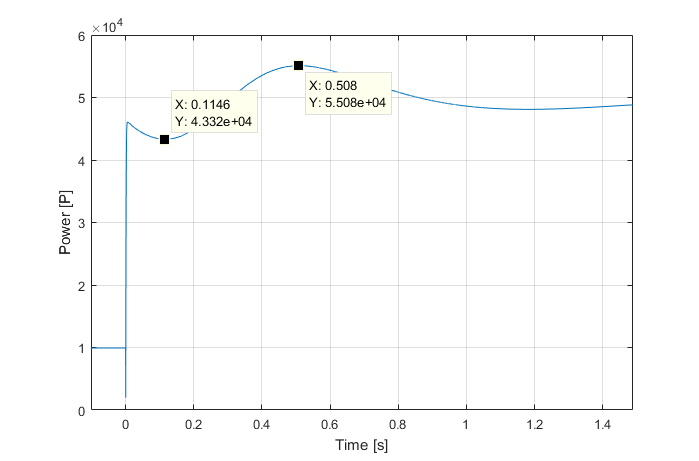
\includegraphics[width=1.1\textwidth]{rapport/billeder/model_estimation_natural_frequency}
% \caption{Step response of the genset from 10 kW to 50 kW}
% \label{fig:gensetdata1}
% \end{figure}

The approach in constructing the TF, is a curvefit from different step sizes. By trial and error it is decided to attempt to fit a second order system to replicate the dynamics of the tenth order genset model. From \figref{fig:stepresponses_simulinkgensetmodel} a step rise is shown when the step is performed on the genset simulink model. To increase the speed of the fitted genset model zeros can be inserted in to the model, and in \figref{fig:stepresponse_zeros} it is shown how one or more zeros affect the model.


\begin{figure}[H]
\centering
%This file was created by matlab2tikz.

%The latest updates can be retrieved from
% http://www.mathworks.com/matlabcentral/fileexchange/22022-matlab2tikz-matlab2tikz
%where you can also make suggestions and rate matlab2tikz.

\definecolor{mycolor1}{rgb}{0.00000,0.44700,0.74100}%
\definecolor{mycolor2}{rgb}{0.85000,0.32500,0.09800}%
\definecolor{mycolor3}{rgb}{0.92900,0.69400,0.12500}%
\definecolor{mycolor4}{rgb}{0.00000,0.00000,0.00000}%

\begin{tikzpicture}

\begin{axis}[%
width=4.521in,
height=3.527in,
at={(0.758in,0.519in)},
scale only axis,
xmin=-0.5,
xmax=2,
xlabel={Time [s]},
xmajorgrids,
ymin=3,
ymax=25,
ylabel={Power [kW]},
ymajorgrids,
axis background/.style={fill=white},
legend style={at={(0.97,0.3)},legend cell align=left,align=left,draw=white!15!black},
y filter/.code={\pgfmathparse{#1/1000}\pgfmathresult}
]
\addplot [color=mycolor1,solid,line width=2.0pt]
 table[row sep=crcr]{%
-1.01	10000.1905778714\\
-1	10000.2059102375\\
-0.99	10000.2188770735\\
-0.98	10000.2294987059\\
-0.97	10000.2378124952\\
-0.96	10000.2438716827\\
-0.95	10000.247744173\\
-0.94	10000.2495112656\\
-0.93	10000.2492663479\\
-0.92	10000.2471135613\\
-0.91	10000.2431664529\\
-0.9	10000.2375466218\\
-0.89	10000.230382374\\
-0.88	10000.2218073924\\
-0.87	10000.2119594342\\
-0.86	10000.2009790623\\
-0.85	10000.1890084197\\
-0.84	10000.1761900544\\
-0.83	10000.1626658006\\
-0.82	10000.1485757222\\
-0.81	10000.1340571237\\
-0.8	10000.119243633\\
-0.79	10000.1042643582\\
-0.78	10000.0892431234\\
-0.77	10000.0742977827\\
-0.76	10000.059539616\\
-0.75	10000.0450728057\\
-0.74	10000.0309939949\\
-0.73	10000.017391926\\
-0.72	10000.0043471585\\
-0.71	9999.99193186446\\
-0.7	9999.98020969841\\
-0.69	9999.96923574018\\
-0.68	9999.95905650619\\
-0.67	9999.94971002636\\
-0.66	9999.9412259824\\
-0.649999999999999	9999.93362590344\\
-0.64	9999.92692341449\\
-0.63	9999.92112453321\\
-0.62	9999.91622801012\\
-0.61	9999.91222570764\\
-0.6	9999.90910301274\\
-0.59	9999.90683927871\\
-0.58	9999.90540829081\\
-0.57	9999.90477875123\\
-0.56	9999.90491477852\\
-0.55	9999.90577641699\\
-0.54	9999.90732015153\\
-0.53	9999.90949942383\\
-0.52	9999.91226514563\\
-0.51	9999.91556620555\\
-0.5	9999.91934996559\\
-0.49	9999.92356274428\\
-0.48	9999.92815028327\\
-0.47	9999.93305819461\\
-0.46	9999.93823238635\\
-0.45	9999.94361946425\\
-0.44	9999.9491671076\\
-0.43	9999.9548244178\\
-0.42	9999.96054223814\\
-0.41	9999.96627344401\\
-0.399999999999999	9999.97197320264\\
-0.39	9999.97759920206\\
-0.38	9999.98311184888\\
-0.37	9999.98847443519\\
-0.36	9999.99365327473\\
-0.35	9999.99861780879\\
-0.34	10000.0033406827\\
-0.33	10000.0077977937\\
-0.32	10000.0119683115\\
-0.31	10000.0158346722\\
-0.3	10000.0193825478\\
-0.29	10000.022600792\\
-0.28	10000.0254813645\\
-0.27	10000.0280192348\\
-0.26	10000.0302122685\\
-0.25	10000.032061096\\
-0.24	10000.0335689675\\
-0.23	10000.0347415947\\
-0.22	10000.0355869817\\
-0.21	10000.0361152467\\
-0.2	10000.0363384368\\
-0.19	10000.0362703374\\
-0.18	10000.0359262768\\
-0.17	10000.0353229307\\
-0.16	10000.0344781247\\
-0.149999999999999	10000.0334106384\\
-0.14	10000.0321400129\\
-0.13	10000.0306863607\\
-0.12	10000.0290701825\\
-0.11	10000.027312189\\
-0.0999999999999996	10000.0254331309\\
-0.0899999999999999	10000.0234536371\\
-0.0800000000000001	10000.0213940616\\
-0.0700000000000003	10000.0192743411\\
-0.0599999999999996	10000.0171138623\\
-0.0499999999999998	10000.0149313407\\
-0.04	10000.0127447105\\
-0.0300000000000002	10000.0105710259\\
-0.0199999999999996	10000.0084263749\\
-0.00999999999999979	10000.0063258039\\
0	10000.0042832554\\
0.00999999999999979	10038.8566005852\\
0.0200000000000005	10152.4737321047\\
0.0300000000000002	10336.1806761712\\
0.04	10585.0000619125\\
0.0499999999999998	10893.7058613137\\
0.0600000000000005	11256.8762871623\\
0.0700000000000003	11668.9455107092\\
0.0800000000000001	12124.2538606035\\
0.0899999999999999	12617.0961935601\\
0.100000000000001	13141.768157035\\
0.11	13692.6100946397\\
0.12	14264.0483758542\\
0.13	14850.6339625412\\
0.14	15447.0780555834\\
0.15	16048.2846954209\\
0.16	16649.3802201468\\
0.17	17245.7395139258\\
0.18	17833.0090066454\\
0.19	18407.1264127197\\
0.2	18964.3372227073\\
0.21	19501.2079857208\\
0.22	20014.6364434014\\
0.23	20501.8585973987\\
0.24	20960.4528117528\\
0.25	21388.3410692703\\
0.26	21783.787516852\\
0.27	22145.3944487629\\
0.28	22472.0958889958\\
0.29	22763.1489441916\\
0.3	23018.1231070339\\
0.310000000000001	23236.8876966871\\
0.32	23419.5976277138\\
0.33	23566.6777020554\\
0.34	23678.8056201519\\
0.350000000000001	23756.8939071745\\
0.36	23802.0709487472\\
0.37	23815.6613275125\\
0.38	23799.1656475592\\
0.39	23754.240028169\\
0.4	23682.675441667\\
0.41	23586.3770624765\\
0.42	23467.343785901\\
0.43	23327.6480657928\\
0.44	23169.4162102288\\
0.45	22994.8092637176\\
0.46	22806.0045934082\\
0.47	22605.1782853803\\
0.48	22394.4884454628\\
0.49	22176.0594872584\\
0.5	21951.9674782444\\
0.51	21724.2266030702\\
0.52	21494.7767915559\\
0.53	21265.4725475125\\
0.54	21038.0730034171\\
0.55	20814.2332152591\\
0.560000000000001	20595.4967015935\\
0.57	20383.2892210458\\
0.58	20178.9137732646\\
0.59	19983.5467996563\\
0.600000000000001	19798.2355521952\\
0.61	19623.8965912155\\
0.62	19461.3153663795\\
0.63	19311.146829003\\
0.64	19173.9170186023\\
0.65	19050.0255619306\\
0.66	18939.7490188746\\
0.67	18843.2450063975\\
0.68	18760.5570292154\\
0.69	18691.6199440737\\
0.7	18636.2659833277\\
0.71	18594.2312629971\\
0.72	18565.1627005345\\
0.73	18548.6252681927\\
0.74	18544.1095090552\\
0.75	18551.0392444789\\
0.76	18568.7794038427\\
0.77	18596.6439100689\\
0.78	18633.9035573311\\
0.79	18679.7938206593\\
0.8	18733.5225407376\\
0.810000000000001	18794.2774310355\\
0.82	18861.2333584679\\
0.83	18933.5593530047\\
0.84	19010.4253060032\\
0.850000000000001	19091.0083214817\\
0.86	19174.4986890413\\
0.87	19260.1054516517\\
0.88	19347.0615459955\\
0.89	19434.6284974961\\
0.9	19522.100656489\\
0.91	19608.8089662237\\
0.92	19694.1242574598\\
0.93	19777.4600683369\\
0.94	19858.2749919197\\
0.95	19936.0745573392\\
0.96	20010.4126537401\\
0.97	20080.8925093012\\
0.98	20147.1672403982\\
0.99	20208.9399885241\\
1	20265.9636648648\\
1.01	20318.0403244356\\
1.02	20365.0201934287\\
1.03	20406.8003748873\\
1.04	20443.3232590279\\
1.05	20474.574665466\\
1.06	20500.5817452844\\
1.07	20521.4106713096\\
1.08	20537.1641451555\\
1.09	20547.9787495511\\
1.1	20554.0221742129\\
1.11	20555.4903430606\\
1.12	20552.6044699208\\
1.13	20545.6080690359\\
1.14	20534.7639457067\\
1.15	20520.3511912599\\
1.16	20502.6622052738\\
1.17	20481.9997666149\\
1.18	20458.6741733705\\
1.19	20433.0004702088\\
1.2	20405.2957800834\\
1.21	20375.8767555364\\
1.22	20345.0571631541\\
1.23	20313.1456130208\\
1.24	20280.4434432905\\
1.25	20247.2427682913\\
1.26	20213.8246968894\\
1.27	20180.4577261834\\
1.28	20147.3963139946\\
1.29	20114.8796320629\\
1.3	20083.1305003701\\
1.31	20052.3545015952\\
1.32	20022.7392733687\\
1.33	19994.4539747425\\
1.34	19967.648922132\\
1.35	19942.4553889206\\
1.36	19918.9855619553\\
1.37	19897.3326472923\\
1.38	19877.5711167941\\
1.39	19859.7570865207\\
1.4	19843.9288173001\\
1.41	19830.107327413\\
1.42	19818.2971069749\\
1.43	19808.4869233414\\
1.44	19800.650706708\\
1.45	19794.7485050052\\
1.46	19790.7274972111\\
1.47	19788.5230543051\\
1.48	19788.0598372706\\
1.49	19789.2529218016\\
1.5	19792.0089396943\\
1.51	19796.2272272808\\
1.52	19801.8009717003\\
1.53	19808.6183462871\\
1.54	19816.5636268816\\
1.55	19825.5182814328\\
1.56	19835.3620258579\\
1.57	19845.9738397371\\
1.58	19857.2329360618\\
1.59	19869.0196798998\\
1.6	19881.2164514963\\
1.61	19893.7084499861\\
1.62	19906.3844345422\\
1.63	19919.1374004325\\
1.64	19931.8651880828\\
1.65	19944.4710238597\\
1.66	19956.8639918769\\
1.67	19968.9594366967\\
1.68	19980.6792973344\\
1.69	19991.9523734863\\
1.7	20002.7145253727\\
1.71	20012.9088090316\\
1.72	20022.4855493007\\
1.73	20031.402353092\\
1.74	20039.6240658925\\
1.75	20047.1226747094\\
1.76	20053.8771609315\\
1.77	20059.873306784\\
1.78	20065.1034592276\\
1.79	20069.5662552818\\
1.8	20073.2663128514\\
1.81	20076.2138911886\\
1.82	20078.4245251521\\
1.83	20079.9186374102\\
1.84	20080.7211326986\\
1.85	20080.8609781691\\
1.86	20080.3707737691\\
1.87	20079.2863164699\\
1.88	20077.6461620111\\
1.89	20075.491187666\\
1.9	20072.8641593429\\
1.91	20069.8093061373\\
1.92	20066.3719052343\\
1.93	20062.5978798329\\
1.94	20058.5334125278\\
1.95	20054.2245763411\\
1.96	20049.7169853512\\
1.97	20045.0554666112\\
1.98	20040.2837548063\\
1.99	20035.4442108435\\
2	20030.5775653269\\
2.01	20025.72268763\\
};
\addlegendentry{No zero};

\addplot [color=mycolor2,solid,line width=2.0pt]
 table[row sep=crcr]{%
-1.01	10000.280374439\\
-1	10000.2828237666\\
-0.99	10000.282969776\\
-0.98	10000.280928402\\
-0.97	10000.2768265386\\
-0.96	10000.2708005046\\
-0.95	10000.2629945142\\
-0.94	10000.2535591652\\
-0.93	10000.2426499537\\
-0.92	10000.2304258277\\
-0.91	10000.2170477873\\
-0.9	10000.2026775395\\
-0.89	10000.187476217\\
-0.88	10000.1716031659\\
-0.87	10000.1552148088\\
-0.86	10000.1384635885\\
-0.85	10000.1214969958\\
-0.84	10000.1044566847\\
-0.83	10000.0874776783\\
-0.82	10000.0706876649\\
-0.81	10000.0542063876\\
-0.8	10000.0381451255\\
-0.79	10000.0226062664\\
-0.78	10000.0076829699\\
-0.77	9999.99345891912\\
-0.76	9999.98000815703\\
-0.75	9999.96739500641\\
-0.74	9999.95567406812\\
-0.73	9999.94489029461\\
-0.72	9999.93507913394\\
-0.71	9999.92626673974\\
-0.7	9999.9184702421\\
-0.69	9999.91169807418\\
-0.68	9999.90595034923\\
-0.67	9999.90121928257\\
-0.66	9999.89748965297\\
-0.649999999999999	9999.89473929781\\
-0.64	9999.89293963663\\
-0.63	9999.89205621746\\
-0.62	9999.89204928063\\
-0.61	9999.89287433488\\
-0.6	9999.89448274048\\
-0.59	9999.89682229488\\
-0.58	9999.89983781588\\
-0.57	9999.90347171822\\
-0.56	9999.90766457929\\
-0.55	9999.91235569033\\
-0.54	9999.91748358948\\
-0.53	9999.92298657356\\
-0.52	9999.92880318564\\
-0.51	9999.93487267603\\
-0.5	9999.94113543433\\
-0.49	9999.94753339077\\
-0.48	9999.95401038524\\
-0.47	9999.96051250292\\
-0.46	9999.96698837553\\
-0.45	9999.97338944758\\
-0.44	9999.97967020757\\
-0.43	9999.98578838385\\
-0.42	9999.99170510564\\
-0.41	9999.99738502961\\
-0.399999999999999	10000.0027964329\\
-0.39	10000.0079112737\\
-0.38	10000.0127052197\\
-0.37	10000.0171576476\\
-0.36	10000.0212516131\\
-0.35	10000.0249737947\\
-0.34	10000.0283144121\\
-0.33	10000.0312671215\\
-0.32	10000.0338288899\\
-0.31	10000.0359998502\\
-0.3	10000.0377831394\\
-0.29	10000.0391847215\\
-0.28	10000.0402131981\\
-0.27	10000.040879608\\
-0.26	10000.0411972182\\
-0.25	10000.0411813086\\
-0.24	10000.0408489521\\
-0.23	10000.0402187916\\
-0.22	10000.0393108168\\
-0.21	10000.0381461417\\
-0.2	10000.0367467849\\
-0.19	10000.035135454\\
-0.18	10000.0333353354\\
-0.17	10000.0313698915\\
-0.16	10000.0292626661\\
-0.149999999999999	10000.0270370986\\
-0.14	10000.024716349\\
-0.13	10000.0223231333\\
-0.12	10000.0198795714\\
-0.11	10000.017407047\\
-0.0999999999999996	10000.01492608\\
-0.0899999999999999	10000.0124562124\\
-0.0800000000000001	10000.0100159079\\
-0.0700000000000003	10000.0076224636\\
-0.0599999999999996	10000.0052919368\\
-0.0499999999999998	10000.0030390841\\
-0.04	10000.0008773135\\
-0.0300000000000002	9999.99881865007\\
-0.0199999999999996	9999.99687371334\\
-0.00999999999999979	9999.99505170702\\
0	9999.99336042002\\
0.00999999999999979	10457.3888834216\\
0.0200000000000005	10965.0536291511\\
0.0300000000000002	11516.5218226282\\
0.04	12105.3188374109\\
0.0499999999999998	12725.0115251396\\
0.0600000000000005	13369.2556676817\\
0.0700000000000003	14031.8403325487\\
0.0800000000000001	14706.7289472604\\
0.0899999999999999	15388.096942972\\
0.100000000000001	16070.3658517232\\
0.11	16748.2337748606\\
0.12	17416.7021723348\\
0.13	18071.0989534716\\
0.14	18707.0978792956\\
0.15	19320.7343143889\\
0.16	19908.4173924583\\
0.17	20466.9386841531\\
0.18	20993.47747812\\
0.19	21485.6028067338\\
0.2	21941.2723663395\\
0.21	22358.8284981543\\
0.22	22736.9914101721\\
0.23	23074.8498325094\\
0.24	23371.8493086193\\
0.25	23627.7783327269\\
0.26	23842.7525497417\\
0.27	24017.1972378377\\
0.28	24151.828295931\\
0.29	24247.6319585114\\
0.3	24305.8434587781\\
0.310000000000001	24327.9248579078\\
0.32	24315.5422536336\\
0.33	24270.5425752613\\
0.34	24194.9301649103\\
0.350000000000001	24090.8433362591\\
0.36	23960.5310925247\\
0.37	23806.3301749486\\
0.38	23630.6426018045\\
0.39	23435.913846037\\
0.4	23224.6117871912\\
0.41	22999.2065604319\\
0.42	22762.1514123041\\
0.43	22515.8646595511\\
0.44	22262.7128339209\\
0.45	22004.995082534\\
0.46	21744.928880181\\
0.47	21484.6370969458\\
0.48	21226.1364519024\\
0.49	20971.3273713937\\
0.5	20721.9852586385\\
0.51	20479.7531701989\\
0.52	20246.1358842265\\
0.53	20022.4953354526\\
0.54	19810.0473826296\\
0.55	19609.8598656084\\
0.560000000000001	19422.851901478\\
0.57	19249.7943622188\\
0.58	19091.31147014\\
0.59	18947.8834420059\\
0.600000000000001	18819.8501081804\\
0.61	18707.4154293589\\
0.62	18610.6528304717\\
0.63	18529.5112691384\\
0.64	18463.8219545899\\
0.65	18413.3056322393\\
0.66	18377.580349034\\
0.67	18356.1696153313\\
0.68	18348.5108802682\\
0.69	18353.9642393986\\
0.7	18371.8212957121\\
0.71	18401.3140979742\\
0.72	18441.6240835988\\
0.73	18491.8909569285\\
0.74	18551.2214378066\\
0.75	18618.6978196375\\
0.76	18693.3862806846\\
0.77	18774.3448971202\\
0.78	18860.6313112519\\
0.79	18951.3100133752\\
0.8	19045.4592007911\\
0.810000000000001	19142.1771826363\\
0.82	19240.588304267\\
0.83	19339.8483699733\\
0.84	19439.1495477435\\
0.850000000000001	19537.7247446163\\
0.86	19634.8514458206\\
0.87	19729.855015376\\
0.88	19822.1114600982\\
0.89	19911.0496629865\\
0.9	19996.1530957531\\
0.91	20076.9610237748\\
0.92	20153.0692199785\\
0.93	20224.1302071184\\
0.94	20289.8530505477\\
0.95	20350.0027259237\\
0.96	20404.3990883232\\
0.97	20452.9154709645\\
0.98	20495.4769431571\\
0.99	20532.0582582181\\
1	20562.6815229205\\
1.01	20587.41362058\\
1.02	20606.363420154\\
1.03	20619.6788037275\\
1.04	20627.5435445169\\
1.05	20630.1740670397\\
1.06	20627.8161203977\\
1.07	20620.741394719\\
1.08	20609.244109712\\
1.09	20593.6376030334\\
1.1	20574.2509447586\\
1.11	20551.4256027129\\
1.12	20525.5121817665\\
1.13	20496.8672584548\\
1.14	20465.850330466\\
1.15	20432.8208986571\\
1.16	20398.1356973446\\
1.17	20362.1460866703\\
1.18	20325.1956188955\\
1.19	20287.6177885313\\
1.2	20249.7339742962\\
1.21	20211.8515790068\\
1.22	20174.2623716714\\
1.23	20137.2410342825\\
1.24	20101.0439141017\\
1.25	20065.9079806036\\
1.26	20032.0499847142\\
1.27	19999.6658165405\\
1.28	19968.9300564499\\
1.29	19939.9957131327\\
1.3	19912.9941411616\\
1.31	19888.0351295628\\
1.32	19865.2071520227\\
1.33	19844.5777685899\\
1.34	19826.1941680774\\
1.35	19810.0838398365\\
1.36	19796.2553631518\\
1.37	19784.6993021978\\
1.38	19775.3891942982\\
1.39	19768.2826191328\\
1.4	19763.3223365397\\
1.41	19760.4374806631\\
1.42	19759.5447983816\\
1.43	19760.5499202277\\
1.44	19763.3486523548\\
1.45	19767.8282785291\\
1.46	19773.8688616077\\
1.47	19781.3445345008\\
1.48	19790.1247712089\\
1.49	19800.0756291538\\
1.5	19811.0609546931\\
1.51	19822.9435444016\\
1.52	19835.5862554213\\
1.53	19848.8530589138\\
1.54	19862.6100313927\\
1.55	19876.726279454\\
1.56	19891.0747941671\\
1.57	19905.5332321176\\
1.58	19919.9846208143\\
1.59	19934.3179868674\\
1.6	19948.428906027\\
1.61	19962.2199748118\\
1.62	19975.601204083\\
1.63	19988.4903354956\\
1.64	20000.8130823111\\
1.65	20012.5032965581\\
1.66	20023.5030649985\\
1.67	20033.7627367763\\
1.68	20043.2408860097\\
1.69	20051.9042129192\\
1.7	20059.7273873795\\
1.71	20066.6928390237\\
1.72	20072.7904982357\\
1.73	20078.0174925212\\
1.74	20082.3778028631\\
1.75	20085.8818847443\\
1.76	20088.5462585518\\
1.77	20090.3930740744\\
1.78	20091.4496537647\\
1.79	20091.7480193649\\
1.8	20091.3244063871\\
1.81	20090.2187708068\\
1.82	20088.4742921648\\
1.83	20086.1368770895\\
1.84	20083.2546670413\\
1.85	20079.8775538579\\
1.86	20076.0567064361\\
1.87	20071.8441116305\\
1.88	20067.2921321826\\
1.89	20062.4530842217\\
1.9	20057.3788365974\\
1.91	20052.1204340199\\
1.92	20046.727745703\\
1.93	20041.249140919\\
1.94	20035.7311925985\\
1.95	20030.2184098325\\
1.96	20024.7529998688\\
1.97	20019.3746599374\\
1.98	20014.1203989927\\
1.99	20009.0243892254\\
2	20004.1178469744\\
2.01	19999.4289424633\\
};
\addlegendentry{One zero};

\addplot [color=mycolor3,solid,line width=2.0pt]
 table[row sep=crcr]{%
-1.01	9999.99153471447\\
-1	9999.99426416361\\
-0.99	9999.99689908438\\
-0.98	9999.99942398183\\
-0.97	10000.0018249961\\
-0.96	10000.0040899261\\
-0.95	10000.0062082391\\
-0.94	10000.0081710675\\
-0.93	10000.0099711917\\
-0.92	10000.011603013\\
-0.91	10000.0130625135\\
-0.9	10000.014347207\\
-0.89	10000.0154560807\\
-0.88	10000.0163895272\\
-0.87	10000.0171492712\\
-0.86	10000.0177382876\\
-0.85	10000.0181607153\\
-0.84	10000.0184217666\\
-0.83	10000.0185276317\\
-0.82	10000.0184853821\\
-0.81	10000.0183028706\\
-0.8	10000.0179886318\\
-0.79	10000.0175517812\\
-0.78	10000.0170019156\\
-0.77	10000.0163490148\\
-0.76	10000.015603345\\
-0.75	10000.0147753657\\
-0.74	10000.0138756386\\
-0.73	10000.0129147414\\
-0.72	10000.0119031855\\
-0.71	10000.0108513385\\
-0.7	10000.0097693513\\
-0.69	10000.0086670913\\
-0.68	10000.0075540803\\
-0.67	10000.0064394392\\
-0.66	10000.005331838\\
-0.649999999999999	10000.0042394518\\
-0.64	10000.0031699227\\
-0.63	10000.0021303288\\
-0.62	10000.0011271575\\
-0.61	10000.000166286\\
-0.6	9999.99925296713\\
-0.59	9999.9983918201\\
-0.58	9999.99758682765\\
-0.57	9999.99684133742\\
-0.56	9999.99615806855\\
-0.55	9999.99553912264\\
-0.54	9999.99498599893\\
-0.53	9999.99449961338\\
-0.52	9999.99408032128\\
-0.51	9999.99372794295\\
-0.5	9999.99344179238\\
-0.49	9999.99322070819\\
-0.48	9999.99306308678\\
-0.47	9999.99296691712\\
-0.46	9999.99292981698\\
-0.45	9999.99294907013\\
-0.44	9999.99302166426\\
-0.43	9999.9931443292\\
-0.42	9999.99331357525\\
-0.41	9999.99352573121\\
-0.399999999999999	9999.99377698188\\
-0.39	9999.99406340479\\
-0.38	9999.99438100583\\
-0.37	9999.99472575371\\
-0.36	9999.99509361288\\
-0.35	9999.99548057482\\
-0.34	9999.99588268759\\
-0.33	9999.99629608337\\
-0.32	9999.99671700397\\
-0.31	9999.99714182427\\
-0.3	9999.99756707329\\
-0.29	9999.99798945319\\
-0.28	9999.99840585583\\
-0.27	9999.99881337706\\
-0.26	9999.99920932878\\
-0.25	9999.9995912486\\
-0.24	9999.9999569074\\
-0.23	10000.0003043146\\
-0.22	10000.0006317214\\
-0.21	10000.000937622\\
-0.2	10000.0012207527\\
-0.19	10000.0014800897\\
-0.18	10000.0017148441\\
-0.17	10000.0019244568\\
-0.16	10000.0021085908\\
-0.149999999999999	10000.0022671224\\
-0.14	10000.0024001315\\
-0.13	10000.0025078904\\
-0.12	10000.0025908524\\
-0.11	10000.0026496384\\
-0.0999999999999996	10000.0026850243\\
-0.0899999999999999	10000.0026979268\\
-0.0800000000000001	10000.002689389\\
-0.0700000000000003	10000.0026605665\\
-0.0599999999999996	10000.0026127121\\
-0.0499999999999998	10000.0025471618\\
-0.04	10000.0024653198\\
-0.0300000000000002	10000.0023686448\\
-0.0199999999999996	10000.0022586352\\
-0.00999999999999979	10000.0021368164\\
0	19645.0020047268\\
0.00999999999999979	19575.3902652351\\
0.0200000000000005	19512.5874841567\\
0.0300000000000002	19456.7314400585\\
0.04	19407.89939253\\
0.0499999999999998	19366.1105626911\\
0.0600000000000005	19331.3289347553\\
0.0700000000000003	19303.4663407506\\
0.0800000000000001	19282.3857902408\\
0.0899999999999999	19267.905006946\\
0.100000000000001	19259.8001345\\
0.11	19257.8095742017\\
0.12	19261.6379184844\\
0.13	19270.9599449386\\
0.14	19285.424637038\\
0.15	19304.6591992389\\
0.16	19328.2730358065\\
0.17	19355.8616645581\\
0.18	19387.010538682\\
0.19	19421.298751859\\
0.2	19458.3026040746\\
0.21	19497.5990077316\\
0.22	19538.7687159383\\
0.23	19581.3993571396\\
0.24	19625.0882625558\\
0.25	19669.4450751744\\
0.26	19714.0941313006\\
0.27	19758.6766078758\\
0.28	19802.8524309266\\
0.29	19846.3019425824\\
0.3	19888.727326088\\
0.310000000000001	19929.8537901331\\
0.32	19969.4305156058\\
0.33	20007.2313695528\\
0.34	20043.0553926737\\
0.350000000000001	20076.7270681068\\
0.36	20108.0963805486\\
0.37	20137.0386759077\\
0.38	20163.4543327124\\
0.39	20187.2682573702\\
0.4	20208.4292161185\\
0.41	20226.9090171154\\
0.42	20242.7015565854\\
0.43	20255.8217432786\\
0.44	20266.3043157139\\
0.45	20274.2025667658\\
0.46	20279.5869901304\\
0.47	20282.5438630682\\
0.48	20283.1737795798\\
0.49	20281.5901478354\\
0.5	20277.9176652484\\
0.51	20272.290784079\\
0.52	20264.8521798687\\
0.53	20255.7512343612\\
0.54	20245.1425438608\\
0.55	20233.1844632272\\
0.560000000000001	20220.0376949119\\
0.57	20205.8639316172\\
0.58	20190.8245603101\\
0.59	20175.0794344552\\
0.600000000000001	20158.7857204608\\
0.61	20142.0968234505\\
0.62	20125.1613966067\\
0.63	20108.122437469\\
0.64	20091.1164737321\\
0.65	20074.2728402651\\
0.66	20057.7130482873\\
0.67	20041.5502468761\\
0.68	20025.8887762632\\
0.69	20010.8238116954\\
0.7	19996.4410960011\\
0.71	19982.8167584147\\
0.72	19970.0172166698\\
0.73	19958.0991588857\\
0.74	19947.1096013289\\
0.75	19937.0860177507\\
0.76	19928.0565356652\\
0.77	19920.040194655\\
0.78	19913.0472615603\\
0.79	19907.0795972352\\
0.8	19902.1310694216\\
0.810000000000001	19898.1880062189\\
0.82	19895.2296845915\\
0.83	19893.2288483703\\
0.84	19892.1522502591\\
0.850000000000001	19891.961212449\\
0.86	19892.6122005779\\
0.87	19894.0574059345\\
0.88	19896.245331002\\
0.89	19899.1213736611\\
0.9	19902.628405621\\
0.91	19906.7073409134\\
0.92	19911.297690577\\
0.93	19916.3380999598\\
0.94	19921.7668653833\\
0.95	19927.5224272388\\
0.96	19933.5438369123\\
0.97	19939.7711952727\\
0.98	19946.1460607903\\
0.99	19952.6118256843\\
1	19959.1140588268\\
1.01	19965.6008144508\\
1.02	19972.0229060229\\
1.03	19978.334144939\\
1.04	19984.491543995\\
1.05	19990.455485852\\
1.06	19996.1898569796\\
1.07	20001.6621477987\\
1.08	20006.8435199706\\
1.09	20011.7088419834\\
1.1	20016.2366943732\\
1.11	20020.4093460823\\
1.12	20024.2127036042\\
1.13	20027.6362346902\\
1.14	20030.6728684975\\
1.15	20033.3188741459\\
1.16	20035.5737197159\\
1.17	20037.4399137686\\
1.18	20038.922831496\\
1.19	20040.0305276227\\
1.2	20040.7735381744\\
1.21	20041.1646732038\\
1.22	20041.2188025329\\
1.23	20040.9526365161\\
1.24	20040.3845037655\\
1.25	20039.5341277066\\
1.26	20038.422403744\\
1.27	20037.0711787234\\
1.28	20035.5030342718\\
1.29	20033.7410754886\\
1.3	20031.8087263428\\
1.31	20029.7295330122\\
1.32	20027.5269762753\\
1.33	20025.2242939429\\
1.34	20022.8443141844\\
1.35	20020.4093004816\\
1.36	20017.9408088126\\
1.37	20015.4595575438\\
1.38	20012.9853103878\\
1.39	20010.5367726636\\
1.4	20008.1315009833\\
1.41	20005.7858263778\\
1.42	20003.5147907714\\
1.43	20001.332096616\\
1.44	19999.2500694039\\
1.45	19997.2796326941\\
1.46	19995.4302952075\\
1.47	19993.7101494786\\
1.48	19992.1258814846\\
1.49	19990.6827906226\\
1.5	19989.3848193521\\
1.51	19988.2345917855\\
1.52	19987.2334604736\\
1.53	19986.3815606093\\
1.54	19985.6778708545\\
1.55	19985.1202799862\\
1.56	19984.7056585511\\
1.57	19984.4299347235\\
1.58	19984.288173567\\
1.59	19984.2746589183\\
1.6	19984.3829771272\\
1.61	19984.6061019145\\
1.62	19984.9364796361\\
1.63	19985.3661142782\\
1.64	19985.8866515387\\
1.65	19986.4894613971\\
1.66	19987.165718612\\
1.67	19987.9064806306\\
1.68	19988.7027624433\\
1.69	19989.5456079608\\
1.7	19990.4261575408\\
1.71	19991.33571134\\
1.72	19992.2657882152\\
1.73	19993.2081799459\\
1.74	19994.1550005995\\
1.75	19995.0987309033\\
1.76	19996.0322575383\\
1.77	19996.9489073073\\
1.78	19997.8424761768\\
1.79	19998.7072532279\\
1.8	19999.5380395916\\
1.81	20000.3301624766\\
1.82	20001.0794844311\\
1.83	20001.782408011\\
1.84	20002.4358760488\\
1.85	20003.0373677483\\
1.86	20003.5848908445\\
1.87	20004.0769700909\\
1.88	20004.5126323486\\
1.89	20004.891388565\\
1.9	20005.2132129388\\
1.91	20005.478519576\\
1.92	20005.688136942\\
1.93	20005.8432804207\\
1.94	20005.9455232877\\
1.95	20005.9967664008\\
1.96	20005.9992069074\\
1.97	20005.9553062605\\
1.98	20005.8677578227\\
1.99	20005.7394543313\\
2	20005.5734554802\\
2.01	20005.3729558629\\
};
\addlegendentry{Two zeros};

\addplot [color=mycolor4,dashed,line width=2.0pt]
 table[row sep=crcr]{%
-1.005	9918.75000010479\\
-1	9918.75000001356\\
-0.995	9918.7499999249\\
-0.99	9918.74999983878\\
-0.984999999999999	9918.74999975517\\
-0.98	9918.74999967406\\
-0.975	9918.74999959538\\
-0.97	9918.7499995191\\
-0.965	9918.74999944524\\
-0.96	9918.74999937374\\
-0.955	9918.74999930455\\
-0.95	9918.74999923769\\
-0.944999999999999	9918.74999917305\\
-0.94	9918.7499991107\\
-0.935	9918.74999905051\\
-0.93	9918.74999899253\\
-0.925	9918.74999893664\\
-0.92	9918.74999888294\\
-0.915	9918.74999883121\\
-0.91	9918.74999878158\\
-0.904999999999999	9918.74999873397\\
-0.899999999999999	9918.74999868827\\
-0.895	9918.74999864459\\
-0.89	9918.74999860283\\
-0.885	9918.74999856285\\
-0.88	9918.74999852476\\
-0.875	9918.74999848851\\
-0.87	9918.74999845409\\
-0.865	9918.74999842129\\
-0.859999999999999	9918.74999839021\\
-0.855	9918.74999836083\\
-0.85	9918.74999833313\\
-0.845	9918.74999830706\\
-0.84	9918.74999828259\\
-0.835	9918.74999825969\\
-0.83	9918.7499982383\\
-0.825	9918.74999821841\\
-0.819999999999999	9918.74999819976\\
-0.815	9918.7499981813\\
-0.81	9918.74999816284\\
-0.805	9918.74999814455\\
-0.8	9918.74999812628\\
-0.795	9918.74999810801\\
-0.79	9918.74999808975\\
-0.785	9918.74999807149\\
-0.779999999999999	9918.74999805324\\
-0.774999999999999	9918.74999803499\\
-0.77	9918.74999801683\\
-0.765	9918.74999799876\\
-0.76	9918.74999798069\\
-0.755	9918.74999796262\\
-0.75	9918.74999794469\\
-0.745	9918.7499979268\\
-0.74	9918.74999790891\\
-0.734999999999999	9918.74999789112\\
-0.73	9918.74999787341\\
-0.725	9918.74999785571\\
-0.72	9918.74999783813\\
-0.715	9918.7499978206\\
-0.71	9918.74999780309\\
-0.705	9918.74999778574\\
-0.7	9918.74999776839\\
-0.694999999999999	9918.74999775114\\
-0.69	9918.74999773397\\
-0.685	9918.74999771681\\
-0.68	9918.74999769982\\
-0.675	9918.74999768283\\
-0.67	9918.74999766594\\
-0.665	9918.74999764914\\
-0.66	9918.74999763234\\
-0.654999999999999	9918.74999761571\\
-0.649999999999999	9918.74999759908\\
-0.645	9918.74999758254\\
-0.64	9918.74999756609\\
-0.635	9918.74999754964\\
-0.63	9918.74999753335\\
-0.625	9918.74999751708\\
-0.62	9918.74999750084\\
-0.615	9918.74999748475\\
-0.609999999999999	9918.74999746865\\
-0.605	9918.74999745261\\
-0.6	9918.74999743669\\
-0.595	9918.74999742077\\
-0.59	9918.74999740488\\
-0.585	9918.74999738915\\
-0.58	9918.7499973734\\
-0.575	9918.74999735766\\
-0.569999999999999	9918.74999734205\\
-0.565	9918.74999732648\\
-0.56	9918.74999731091\\
-0.555	9918.74999729535\\
-0.55	9918.7499972799\\
-0.545	9918.74999726451\\
-0.54	9918.74999724912\\
-0.535	9918.74999723374\\
-0.529999999999999	9918.74999721835\\
-0.524999999999999	9918.74999720303\\
-0.52	9918.74999718782\\
-0.515	9918.74999717261\\
-0.51	9918.7499971574\\
-0.505	9918.74999714219\\
-0.5	9918.74999712698\\
-0.495	9918.74999711178\\
-0.49	9918.74999709657\\
-0.484999999999999	9918.74999708135\\
-0.48	9918.74999706632\\
-0.475	9918.74999705129\\
-0.47	9918.74999703626\\
-0.465	9918.74999702122\\
-0.46	9918.74999700619\\
-0.455	9918.74999699115\\
-0.45	9918.74999697613\\
-0.444999999999999	9918.7499969611\\
-0.44	9918.74999694607\\
-0.435	9918.74999693104\\
-0.43	9918.74999691601\\
-0.425	9918.74999690097\\
-0.42	9918.74999688594\\
-0.415	9918.74999687091\\
-0.41	9918.74999685588\\
-0.404999999999999	9918.74999684085\\
-0.399999999999999	9918.74999682582\\
-0.395	9918.74999681073\\
-0.39	9918.74999679552\\
-0.385	9918.74999678031\\
-0.38	9918.74999676511\\
-0.375	9918.7499967499\\
-0.37	9918.74999673469\\
-0.365	9918.74999671949\\
-0.359999999999999	9918.74999670428\\
-0.355	9918.74999668907\\
-0.35	9918.74999667387\\
-0.345	9918.74999665866\\
-0.34	9918.74999664345\\
-0.335	9918.74999662824\\
-0.33	9918.74999661304\\
-0.325	9918.74999659769\\
-0.319999999999999	9918.7499965823\\
-0.315	9918.74999656691\\
-0.31	9918.74999655154\\
-0.305	9918.74999653615\\
-0.3	9918.74999652077\\
-0.295	9918.74999650538\\
-0.29	9918.74999649\\
-0.285	9918.74999647461\\
-0.279999999999999	9918.74999645923\\
-0.274999999999999	9918.74999644384\\
-0.27	9918.74999642846\\
-0.265	9918.74999641304\\
-0.26	9918.74999639748\\
-0.255	9918.74999638192\\
-0.25	9918.74999636636\\
-0.245	9918.7499963508\\
-0.24	9918.74999633525\\
-0.234999999999999	9918.74999631968\\
-0.23	9918.74999630412\\
-0.225	9918.74999628855\\
-0.22	9918.749996273\\
-0.215	9918.74999625744\\
-0.21	9918.74999624187\\
-0.205	9918.74999622631\\
-0.2	9918.74999621075\\
-0.194999999999999	9918.74999619519\\
-0.19	9918.74999617963\\
-0.185	9918.74999616407\\
-0.18	9918.74999614851\\
-0.175	9918.74999613294\\
-0.17	9918.74999611739\\
-0.165	9918.74999610182\\
-0.16	9918.74999608626\\
-0.154999999999999	9918.7499960707\\
-0.149999999999999	9918.74999605513\\
-0.145	9918.74999603947\\
-0.14	9918.74999602374\\
-0.135	9918.749996008\\
-0.13	9918.74999599226\\
-0.125	9918.74999597652\\
-0.12	9918.74999596078\\
-0.114999999999999	9918.74999594505\\
-0.109999999999999	9918.74999592931\\
-0.105	9918.74999591357\\
-0.0999999999999996	9918.74999589791\\
-0.0949999999999998	9918.74999588235\\
-0.0899999999999999	9918.74999586678\\
-0.085	9918.74999585122\\
-0.0800000000000001	9918.74999583566\\
-0.0750000000000002	9918.7499958201\\
-0.0699999999999994	9918.74999580454\\
-0.0649999999999995	9918.74999578898\\
-0.0599999999999996	9918.74999577341\\
-0.0549999999999997	9918.74999575785\\
-0.0499999999999998	9918.74999574229\\
-0.0449999999999999	9918.74999572673\\
-0.04	9918.74999586238\\
-0.0350000000000001	9918.74999609978\\
-0.0299999999999994	9918.74999634002\\
-0.0249999999999995	9918.74999657922\\
-0.0199999999999996	9918.7499968166\\
-0.0149999999999997	9918.74999705208\\
-0.00999999999999979	9918.74999728515\\
-0.00499999999999989	9918.74999751588\\
0	4959.37499887307\\
0.00499999999999989	19558.266776462\\
0.0100000000000007	19533.0431123617\\
0.0150000000000006	19507.1303821087\\
0.0200000000000005	19481.4220231357\\
0.0250000000000004	19456.3415258053\\
0.0300000000000002	19432.1053785717\\
0.0350000000000001	19408.8392713296\\
0.04	19386.6297278293\\
0.0449999999999999	19365.5464363551\\
0.0499999999999998	19345.6514029385\\
0.0550000000000006	19327.0022798386\\
0.0600000000000005	19309.6532062042\\
0.0650000000000004	19293.6546615803\\
0.0700000000000003	19279.0529952666\\
0.0750000000000002	19265.889914154\\
0.0800000000000001	19254.2020404598\\
0.085	19244.0205750349\\
0.0899999999999999	19235.371069571\\
0.0950000000000006	19228.273298232\\
0.100000000000001	19222.7412151105\\
0.105	19218.7829834988\\
0.11	19216.401064043\\
0.115	19215.5923504066\\
0.12	19216.3483427044\\
0.125	19218.6553504753\\
0.13	19222.4947183062\\
0.135000000000001	19227.8430683858\\
0.140000000000001	19234.6725552523\\
0.145	19242.9511288436\\
0.15	19252.6428026618\\
0.155	19263.7079244558\\
0.16	19276.1034473184\\
0.165	19289.7831995024\\
0.17	19304.6981515972\\
0.175	19320.7966799858\\
0.180000000000001	19338.0248257277\\
0.185000000000001	19356.3265481956\\
0.19	19375.6439729424\\
0.195	19395.9176333944\\
0.2	19417.086706055\\
0.205	19439.0892389823\\
0.21	19461.8623733526\\
0.215	19485.3425579718\\
0.220000000000001	19509.4657566211\\
0.225000000000001	19534.1676481516\\
0.23	19559.383819256\\
0.235	19585.0499498583\\
0.24	19611.1019910683\\
0.245	19637.4763356553\\
0.25	19664.1099809963\\
0.255	19690.9406844596\\
0.260000000000001	19717.9071111836\\
0.265000000000001	19744.9489742169\\
0.27	19772.0071669868\\
0.275	19799.0238880688\\
0.28	19825.9427582335\\
0.285	19852.7089297576\\
0.29	19879.2691879874\\
0.295	19905.5720451594\\
0.3	19931.5678264875\\
0.305000000000001	19957.2087485414\\
0.310000000000001	19982.4489899511\\
0.315	20007.2447544891\\
0.32	20031.5543265923\\
0.325	20055.338119406\\
0.33	20078.558715443\\
0.335	20101.1808999711\\
0.34	20123.171687256\\
0.345000000000001	20144.5003398049\\
0.350000000000001	20165.1383807697\\
0.355	20185.0595996881\\
0.36	20204.2400517527\\
0.365	20222.6580508168\\
0.37	20240.2941563551\\
0.375	20257.1311546158\\
0.38	20273.1540342092\\
0.385000000000001	20288.3499563903\\
0.390000000000001	20302.7082203033\\
0.395	20316.2202234649\\
0.4	20328.8794177698\\
0.405	20340.6812613095\\
0.41	20351.6231662995\\
0.415	20361.7044434145\\
0.42	20370.9262428326\\
0.425	20379.2914922911\\
0.430000000000001	20386.8048324574\\
0.435000000000001	20393.4725499133\\
0.44	20399.3025080535\\
0.445	20404.3040761895\\
0.45	20408.4880571509\\
0.455	20411.8666136643\\
0.46	20414.4531937872\\
0.465	20416.2624556655\\
0.470000000000001	20417.310191871\\
0.475000000000001	20417.6132535718\\
0.48	20417.189474773\\
0.485	20416.0575968572\\
0.49	20414.2371936417\\
0.495	20411.7485971592\\
0.5	20408.6128243551\\
0.505	20404.851504883\\
0.510000000000001	20400.4868101685\\
0.515000000000001	20395.5413838971\\
0.52	20390.0382740716\\
0.525	20384.0008667695\\
0.53	20377.4528217209\\
0.535	20370.4180098139\\
0.54	20362.9204526231\\
0.545	20354.9842640436\\
0.55	20346.633594104\\
0.555000000000001	20337.8925750191\\
0.560000000000001	20328.7852695319\\
0.565	20319.3356215867\\
0.57	20309.567409361\\
0.575	20299.5042006802\\
0.58	20289.1693108242\\
0.585	20278.5857627312\\
0.59	20267.7762495939\\
0.595000000000001	20256.7630998356\\
0.600000000000001	20245.5682444485\\
0.605	20234.2131866679\\
0.61	20222.7189739521\\
0.615	20211.1061722304\\
0.62	20199.3948423789\\
0.625	20187.6045188766\\
0.63	20175.7541905926\\
0.635000000000001	20163.8622836509\\
0.640000000000001	20151.9466463144\\
0.645	20140.0245358306\\
0.65	20128.1126071746\\
0.655	20116.2269036278\\
0.66	20104.3828491244\\
0.665	20092.5952422998\\
0.67	20080.8782521726\\
0.675000000000001	20069.2454153915\\
0.680000000000001	20057.709634978\\
0.685000000000001	20046.2831804947\\
0.69	20034.9776895713\\
0.695	20023.8041707179\\
0.7	20012.7730073574\\
0.705	20001.8939630098\\
0.71	19991.1761875591\\
0.715	19980.6282245396\\
0.720000000000001	19970.2580193739\\
0.725000000000001	19960.0729284997\\
0.73	19950.0797293229\\
0.735	19940.2846309357\\
0.74	19930.6932855392\\
0.745	19921.3108005136\\
0.75	19912.1417510783\\
0.755	19903.1901934872\\
0.760000000000001	19894.4596787062\\
0.765000000000001	19885.9532665213\\
0.77	19877.6735400265\\
0.775	19869.6226204448\\
0.78	19861.8021822351\\
0.785	19854.2134684402\\
0.79	19846.8573062334\\
0.795	19839.7341226229\\
0.800000000000001	19832.843960273\\
0.805000000000001	19826.186493407\\
0.810000000000001	19819.7610437525\\
0.815	19813.5665964983\\
0.82	19807.6018162265\\
0.825	19801.865062792\\
0.83	19796.3544071176\\
0.835	19791.0676468774\\
0.84	19786.0023220429\\
0.845000000000001	19781.1557302651\\
0.850000000000001	19776.5249420709\\
0.855	19772.1068158505\\
0.86	19767.8980126162\\
0.865	19763.8950105116\\
0.87	19760.094119056\\
0.875	19756.4914931042\\
0.88	19753.0831465087\\
0.885000000000001	19749.8649654691\\
0.890000000000001	19746.8327215564\\
0.895	19743.982084399\\
0.9	19741.3086340219\\
0.905	19738.8078728279\\
0.91	19736.4752372133\\
0.915	19734.3061088099\\
0.92	19732.2958253477\\
0.925000000000001	19730.4396911325\\
0.930000000000001	19728.7329871343\\
0.935000000000001	19727.1709806821\\
0.94	19725.7489347638\\
0.945	19724.4621169282\\
0.95	19723.3058077888\\
0.955	19722.2753091292\\
0.96	19721.3659516107\\
0.965	19720.5731020835\\
0.970000000000001	19719.8921705027\\
0.975000000000001	19719.3186164541\\
0.98	19718.8479552904\\
0.985	19718.4757638839\\
0.99	19718.1976859994\\
0.995	19718.0094372929\\
1	19717.906809941\\
1.005	19717.8856769083\\
1.01	19717.9419958591\\
1.015	19718.0718127197\\
1.02	19718.2712649003\\
1.025	19718.5365841832\\
1.03	19718.8640992857\\
1.035	19719.2502381077\\
1.04	19719.6915296705\\
1.045	19720.1846057584\\
1.05	19720.7262022706\\
1.055	19721.3131602944\\
1.06	19721.9424269085\\
1.065	19722.6110557271\\
1.07	19723.3162071946\\
1.075	19724.055148641\\
1.08	19724.8252541092\\
1.085	19725.6240039623\\
1.09	19726.4489842849\\
1.095	19727.2978860849\\
1.1	19728.1685043098\\
1.105	19729.0587366847\\
1.11	19729.9665823852\\
1.115	19730.8901405527\\
1.12	19731.8276086656\\
1.125	19732.7772807727\\
1.13	19733.7375456016\\
1.135	19734.7068845513\\
1.14	19735.6838695773\\
1.145	19736.6671609806\\
1.15	19737.6555051085\\
1.155	19738.6477319772\\
1.16	19739.6427528242\\
1.165	19740.6395575998\\
1.17	19741.6372124065\\
1.175	19742.6348568931\\
1.18	19743.6317016131\\
1.185	19744.6270253536\\
1.19	19745.6201724436\\
1.195	19746.6105500469\\
1.2	19747.597625449\\
1.205	19748.5809233423\\
1.21	19749.5600231166\\
1.215	19750.534556162\\
1.22	19751.5042031884\\
1.225	19752.4686915679\\
1.23	19753.4277927047\\
1.235	19754.3813194386\\
1.24	19755.3291234845\\
1.245	19756.2710929145\\
1.25	19757.207149685\\
1.255	19758.1372472131\\
1.26	19759.0613680061\\
1.265	19759.9795213463\\
1.27	19760.8917410353\\
1.275	19761.7980831986\\
1.28	19762.698624155\\
1.285	19763.5934583517\\
1.29	19764.4826963665\\
1.295	19765.36646298\\
1.3	19766.2448953184\\
1.305	19767.1181410682\\
1.31	19767.9863567637\\
1.315	19768.8497061481\\
1.32	19769.708358609\\
1.325	19770.5624876877\\
1.33	19771.4122696639\\
1.335	19772.2578822138\\
1.34	19773.0995031439\\
1.345	19773.9373091973\\
1.35	19774.7714749342\\
1.355	19775.6021716849\\
1.36	19776.4295665744\\
1.365	19777.2538216175\\
1.37	19778.0750928848\\
1.375	19778.8935297358\\
1.38	19779.7092741201\\
1.385	19780.5224599437\\
1.39	19781.3332125002\\
1.395	19782.1416479641\\
1.4	19782.9478729451\\
1.405	19783.7519841014\\
1.41	19784.5540678111\\
1.415	19785.3541998978\\
1.42	19786.1524454111\\
1.425	19786.9488584572\\
1.43	19787.7434820805\\
1.435	19788.5363481914\\
1.44	19789.3274775402\\
1.445	19790.1168797346\\
1.45	19790.9045532979\\
1.455	19791.6904857662\\
1.46	19792.4746538233\\
1.465	19793.2570234702\\
1.47	19794.0375502272\\
1.475	19794.8161793671\\
1.48	19795.5928461772\\
1.485	19796.3674762472\\
1.49	19797.1399857826\\
1.495	19797.9102819403\\
1.5	19798.6782631847\\
1.505	19799.4438196632\\
1.51	19800.2068335975\\
1.515	19800.9671796912\\
1.52	19801.7247255494\\
1.525	19802.4793321104\\
1.53	19803.2308540871\\
1.535	19803.9791404164\\
1.54	19804.7240347148\\
1.545	19805.4653757396\\
1.55	19806.2029978527\\
1.555	19806.9367314866\\
1.56	19807.6664036118\\
1.565	19808.3918382022\\
1.57	19809.1128566991\\
1.575	19809.8292784723\\
1.58	19810.5409212759\\
1.585	19811.2476016997\\
1.59	19811.9491356133\\
1.595	19812.6453386031\\
1.6	19813.3360264004\\
1.605	19814.021015301\\
1.61	19814.7001225745\\
1.615	19815.3731668618\\
1.62	19816.0399685631\\
1.625	19816.7003502121\\
1.63	19817.3541368379\\
1.635	19818.0011563142\\
1.64	19818.6412396948\\
1.645	19819.2742215341\\
1.65	19819.8999401946\\
1.655	19820.5182381384\\
1.66	19821.1289622046\\
1.665	19821.7319638708\\
1.67	19822.3270994998\\
1.675	19822.9142305707\\
1.68	19823.4932238937\\
1.685	19824.0639518107\\
1.69	19824.6262923787\\
1.695	19825.180129539\\
1.7	19825.7253532697\\
1.705	19826.261859724\\
1.71	19826.789551352\\
1.715	19827.3083370087\\
1.72	19827.8181320462\\
1.725	19828.3188583913\\
1.73	19828.8104446095\\
1.735	19829.2928259538\\
1.74	19829.7659444009\\
1.745	19830.229748673\\
1.75	19830.6841942466\\
1.755	19831.1292433491\\
1.76	19831.5648649427\\
1.765	19831.9910346956\\
1.77	19832.4077349435\\
1.775	19832.8149546379\\
1.78	19833.2126892845\\
1.785	19833.6009408721\\
1.79	19833.9797177906\\
1.795	19834.3490347399\\
1.8	19834.7089126302\\
1.805	19835.0593784736\\
1.81	19835.4004652677\\
1.815	19835.7322118721\\
1.82	19836.0546628773\\
1.825	19836.3678684675\\
1.83	19836.6718842768\\
1.835	19836.9667712402\\
1.84	19837.2525954395\\
1.845	19837.5294279438\\
1.85	19837.7973446468\\
1.855	19838.056426099\\
1.86	19838.3067573374\\
1.865	19838.5484277123\\
1.87	19838.7815307107\\
1.875	19839.0061637785\\
1.88	19839.2224281402\\
1.885	19839.430428618\\
1.89	19839.6302734493\\
1.895	19839.8220741038\\
1.9	19840.0059451006\\
1.905	19840.1820038248\\
1.91	19840.3503703453\\
1.915	19840.5111672328\\
1.92	19840.6645193792\\
1.925	19840.8105538178\\
1.93	19840.9493995459\\
1.935	19841.0811873486\\
1.94	19841.2060496254\\
1.945	19841.3241202189\\
1.95	19841.4355342454\\
1.955	19841.54042793\\
1.96	19841.6389384432\\
1.965	19841.7312037414\\
1.97	19841.8173624108\\
1.975	19841.8975535149\\
1.98	19841.9719164452\\
1.985	19842.0405907765\\
1.99	19842.1037161259\\
1.995	19842.1614320155\\
2	19842.2138777399\\
2.005	19842.2611922374\\
};
\addlegendentry{Genset};

\end{axis}
\end{tikzpicture}%
\caption{Step response of second order systems with and without zeros compared with a step from 10 kW to 20 kW on the genset simulink model.}
\label{fig:stepresponse_zeros}
\end{figure}

By adding two zeros to the TF a closer fit can be achieved to the step performed on the genset simulink model. While the second order system is not a perfect match, it is deemed sufficiently close for further progress in parameter estimation and is shown in \eqref{eq:tf_two_zeros}.
%
%
\begin{equation}
\label{eq:tf_two_zeros}
G_1(s) = \frac {b_2 \cdot s^2 + b_1 \cdot s+\omega_n ^2}{s^2+2\cdot \zeta \cdot \omega_n \cdot s + \omega_n ^2} \unit{\cdot}
\end{equation}    

To estimate the parameters senstool is used to get a curve fit of the data from the genset simulink model. First the natural frequency $\omega_n$ is estimated from the data. A half period of the natural frequency is found as shown in \figref{fig:stepresponse_power_10_50kW} and from that the natural frequency is derrived to be 8 $rad/s$, and is used as an initial guess. 
\begin{figure}[H]
\centering
% This file was created by matlab2tikz.
%
%The latest updates can be retrieved from
%  http://www.mathworks.com/matlabcentral/fileexchange/22022-matlab2tikz-matlab2tikz
%where you can also make suggestions and rate matlab2tikz.
%
\definecolor{mycolor1}{rgb}{0.00000,0.44700,0.74100}%
%
\begin{tikzpicture}

\begin{axis}[%
width=4.521in,
height=3.566in,
at={(0.758in,0.481in)},
scale only axis,
xmin=-1,
xmax=3,
xlabel={Time[s]},
xmajorgrids,
ymin=0,
ymax=60,
ylabel={Power[kW]},
ymajorgrids,
axis background/.style={fill=white},
y filter/.code={\pgfmathparse{#1/1000}\pgfmathresult}
]
\addplot [color=black,line width=2.0pt,mark size=2pt,only marks,mark=square*,mark options={solid,fill=black},forget plot]
  table[row sep=crcr]{%
0.1145	43320.106178759\\
};
\node[below right, align=left, text=black, draw=black,  fill=white,rounded corners=2pt,inner sep=1pt]
at (rel axis cs:0.253,0.7) {X: 0.1146 \\ Y: 43.32 };%$\cdot 10^4$

%%-----------------------------------------------------------------------------------------------------------------------

\addplot [color=black,line width=2.0pt,mark size=2pt,only marks,mark=square*,mark options={solid,fill=black},forget plot]
  table[row sep=crcr]{%
0.5079	55082.0445358227\\
};
\node[below right, align=left, text=black, draw=black,  fill=white,rounded corners=2pt,inner sep=1pt]
at (rel axis cs:0.42,0.98) {X: 0.508 \\ Y: 55.08 };%$\cdot 10^4$

\addplot [color=mycolor1,solid,forget plot]
  table[row sep=crcr]{%
-1.01	9919\\
-1	9919\\
-0.99	9919\\
-0.98	9919\\
-0.97	9919\\
-0.96	9919\\
-0.95	9919\\
-0.94	9919\\
-0.93	9919\\
-0.92	9919\\
-0.91	9919\\
-0.9	9919\\
-0.89	9919\\
-0.88	9919\\
-0.87	9919\\
-0.86	9919\\
-0.85	9919\\
-0.84	9919\\
-0.83	9919\\
-0.82	9919\\
-0.81	9919\\
-0.8	9919\\
-0.79	9919\\
-0.78	9919\\
-0.77	9919\\
-0.76	9919\\
-0.75	9919\\
-0.74	9919\\
-0.73	9919\\
-0.72	9919\\
-0.71	9919\\
-0.7	9919\\
-0.69	9919\\
-0.68	9919\\
-0.67	9919\\
-0.66	9919\\
-0.65	9919\\
-0.64	9919\\
-0.63	9919\\
-0.62	9919\\
-0.61	9919\\
-0.6	9919\\
-0.59	9919\\
-0.58	9919\\
-0.57	9919\\
-0.56	9919\\
-0.55	9919\\
-0.54	9919\\
-0.53	9919\\
-0.52	9919\\
-0.51	9919\\
-0.5	9919\\
-0.49	9919\\
-0.48	9919\\
-0.47	9919\\
-0.46	9919\\
-0.45	9919\\
-0.44	9919\\
-0.43	9919\\
-0.42	9919\\
-0.41	9919\\
-0.4	9919\\
-0.39	9919\\
-0.38	9919\\
-0.37	9919\\
-0.36	9919\\
-0.35	9919\\
-0.34	9919\\
-0.33	9919\\
-0.32	9919\\
-0.31	9919\\
-0.3	9919\\
-0.29	9919\\
-0.28	9919\\
-0.27	9919\\
-0.26	9919\\
-0.25	9919\\
-0.24	9919\\
-0.23	9919\\
-0.22	9919\\
-0.21	9919\\
-0.2	9919\\
-0.19	9919\\
-0.18	9919\\
-0.17	9919\\
-0.16	9919\\
-0.15	9919\\
-0.14	9919\\
-0.13	9919\\
-0.12	9919\\
-0.11	9919\\
-0.1	9919\\
-0.09	9919\\
-0.08	9919\\
-0.07	9919\\
-0.06	9919\\
-0.05	9919\\
-0.04	9919\\
-0.03	9919\\
-0.02	9919\\
-0.01	9919\\
0	1984\\
0.01	4.59e+04\\
0.02	4.542e+04\\
0.03	4.5e+04\\
0.04	4.464e+04\\
0.05	4.432e+04\\
0.06	4.405e+04\\
0.07	4.382e+04\\
0.08	4.363e+04\\
0.09	4.348e+04\\
0.1	4.338e+04\\
0.11	4.333e+04\\
0.12	4.332e+04\\
0.13	4.337e+04\\
0.14	4.346e+04\\
0.15	4.36e+04\\
0.16	4.378e+04\\
0.17	4.401e+04\\
0.18	4.428e+04\\
0.19	4.458e+04\\
0.2	4.493e+04\\
0.21	4.53e+04\\
0.22	4.57e+04\\
0.23	4.613e+04\\
0.24	4.658e+04\\
0.25	4.704e+04\\
0.26	4.752e+04\\
0.27	4.8e+04\\
0.28	4.849e+04\\
0.29	4.898e+04\\
0.3	4.947e+04\\
0.31	4.995e+04\\
0.32	5.042e+04\\
0.33	5.088e+04\\
0.34	5.133e+04\\
0.35	5.175e+04\\
0.36	5.216e+04\\
0.37	5.254e+04\\
0.38	5.29e+04\\
0.39	5.323e+04\\
0.4	5.354e+04\\
0.41	5.382e+04\\
0.42	5.407e+04\\
0.43	5.429e+04\\
0.44	5.448e+04\\
0.45	5.465e+04\\
0.46	5.478e+04\\
0.47	5.49e+04\\
0.48	5.498e+04\\
0.49	5.504e+04\\
0.5	5.507e+04\\
0.51	5.508e+04\\
0.52	5.507e+04\\
0.53	5.504e+04\\
0.54	5.499e+04\\
0.55	5.492e+04\\
0.56	5.483e+04\\
0.57	5.473e+04\\
0.58	5.462e+04\\
0.59	5.449e+04\\
0.6	5.435e+04\\
0.61	5.421e+04\\
0.62	5.405e+04\\
0.63	5.388e+04\\
0.64	5.371e+04\\
0.65	5.354e+04\\
0.66	5.336e+04\\
0.67	5.318e+04\\
0.68	5.299e+04\\
0.69	5.281e+04\\
0.7	5.262e+04\\
0.71	5.243e+04\\
0.72	5.225e+04\\
0.73	5.206e+04\\
0.74	5.188e+04\\
0.75	5.17e+04\\
0.76	5.153e+04\\
0.77	5.135e+04\\
0.78	5.118e+04\\
0.79	5.101e+04\\
0.8	5.085e+04\\
0.81	5.069e+04\\
0.82	5.054e+04\\
0.83	5.039e+04\\
0.84	5.025e+04\\
0.85	5.011e+04\\
0.86	4.997e+04\\
0.87	4.985e+04\\
0.88	4.972e+04\\
0.89	4.96e+04\\
0.9	4.949e+04\\
0.91	4.938e+04\\
0.92	4.928e+04\\
0.93	4.918e+04\\
0.94	4.908e+04\\
0.95	4.9e+04\\
0.96	4.891e+04\\
0.97	4.883e+04\\
0.98	4.876e+04\\
0.99	4.869e+04\\
1	4.862e+04\\
1.01	4.856e+04\\
1.02	4.851e+04\\
1.03	4.845e+04\\
1.04	4.841e+04\\
1.05	4.836e+04\\
1.06	4.832e+04\\
1.07	4.829e+04\\
1.08	4.825e+04\\
1.09	4.822e+04\\
1.1	4.82e+04\\
1.11	4.818e+04\\
1.12	4.816e+04\\
1.13	4.814e+04\\
1.14	4.813e+04\\
1.15	4.812e+04\\
1.16	4.811e+04\\
1.17	4.811e+04\\
1.18	4.811e+04\\
1.19	4.811e+04\\
1.2	4.811e+04\\
1.21	4.812e+04\\
1.22	4.812e+04\\
1.23	4.813e+04\\
1.24	4.814e+04\\
1.25	4.816e+04\\
1.26	4.817e+04\\
1.27	4.819e+04\\
1.28	4.821e+04\\
1.29	4.823e+04\\
1.3	4.825e+04\\
1.31	4.828e+04\\
1.32	4.83e+04\\
1.33	4.833e+04\\
1.34	4.835e+04\\
1.35	4.838e+04\\
1.36	4.841e+04\\
1.37	4.844e+04\\
1.38	4.847e+04\\
1.39	4.85e+04\\
1.4	4.853e+04\\
1.41	4.857e+04\\
1.42	4.86e+04\\
1.43	4.863e+04\\
1.44	4.866e+04\\
1.45	4.87e+04\\
1.46	4.873e+04\\
1.47	4.876e+04\\
1.48	4.88e+04\\
1.49	4.883e+04\\
1.5	4.887e+04\\
1.51	4.89e+04\\
1.52	4.893e+04\\
1.53	4.897e+04\\
1.54	4.9e+04\\
1.55	4.903e+04\\
1.56	4.906e+04\\
1.57	4.909e+04\\
1.58	4.913e+04\\
1.59	4.916e+04\\
1.6	4.919e+04\\
1.61	4.922e+04\\
1.62	4.925e+04\\
1.63	4.927e+04\\
1.64	4.93e+04\\
1.65	4.933e+04\\
1.66	4.935e+04\\
1.67	4.938e+04\\
1.68	4.941e+04\\
1.69	4.943e+04\\
1.7	4.945e+04\\
1.71	4.948e+04\\
1.72	4.95e+04\\
1.73	4.952e+04\\
1.74	4.954e+04\\
1.75	4.956e+04\\
1.76	4.958e+04\\
1.77	4.959e+04\\
1.78	4.961e+04\\
1.79	4.963e+04\\
1.8	4.964e+04\\
1.81	4.966e+04\\
1.82	4.967e+04\\
1.83	4.968e+04\\
1.84	4.97e+04\\
1.85	4.971e+04\\
1.86	4.972e+04\\
1.87	4.973e+04\\
1.88	4.974e+04\\
1.89	4.975e+04\\
1.9	4.976e+04\\
1.91	4.976e+04\\
1.92	4.977e+04\\
1.93	4.978e+04\\
1.94	4.978e+04\\
1.95	4.979e+04\\
1.96	4.979e+04\\
1.97	4.979e+04\\
1.98	4.98e+04\\
1.99	4.98e+04\\
2	4.98e+04\\
2.01	4.98e+04\\
2.02	4.98e+04\\
2.03	4.98e+04\\
2.04	4.98e+04\\
2.05	4.98e+04\\
2.06	4.98e+04\\
2.07	4.98e+04\\
2.08	4.98e+04\\
2.09	4.98e+04\\
2.1	4.979e+04\\
2.11	4.979e+04\\
2.12	4.979e+04\\
2.13	4.979e+04\\
2.14	4.978e+04\\
2.15	4.978e+04\\
2.16	4.977e+04\\
2.17	4.977e+04\\
2.18	4.977e+04\\
2.19	4.976e+04\\
2.2	4.976e+04\\
2.21	4.975e+04\\
2.22	4.975e+04\\
2.23	4.974e+04\\
2.24	4.974e+04\\
2.25	4.973e+04\\
2.26	4.973e+04\\
2.27	4.972e+04\\
2.28	4.972e+04\\
2.29	4.971e+04\\
2.3	4.971e+04\\
2.31	4.97e+04\\
2.32	4.969e+04\\
2.33	4.969e+04\\
2.34	4.968e+04\\
2.35	4.968e+04\\
2.36	4.967e+04\\
2.37	4.967e+04\\
2.38	4.966e+04\\
2.39	4.966e+04\\
2.4	4.965e+04\\
2.41	4.965e+04\\
2.42	4.964e+04\\
2.43	4.964e+04\\
2.44	4.963e+04\\
2.45	4.963e+04\\
2.46	4.963e+04\\
2.47	4.962e+04\\
2.48	4.962e+04\\
2.49	4.961e+04\\
2.5	4.961e+04\\
2.51	4.961e+04\\
2.52	4.96e+04\\
2.53	4.96e+04\\
2.54	4.959e+04\\
2.55	4.959e+04\\
2.56	4.959e+04\\
2.57	4.959e+04\\
2.58	4.958e+04\\
2.59	4.958e+04\\
2.6	4.958e+04\\
2.61	4.957e+04\\
2.62	4.957e+04\\
2.63	4.957e+04\\
2.64	4.957e+04\\
2.65	4.957e+04\\
2.66	4.956e+04\\
2.67	4.956e+04\\
2.68	4.956e+04\\
2.69	4.956e+04\\
2.7	4.956e+04\\
2.71	4.956e+04\\
2.72	4.956e+04\\
2.73	4.955e+04\\
2.74	4.955e+04\\
2.75	4.955e+04\\
2.76	4.955e+04\\
2.77	4.955e+04\\
2.78	4.955e+04\\
2.79	4.955e+04\\
2.8	4.955e+04\\
2.81	4.955e+04\\
2.82	4.955e+04\\
2.83	4.955e+04\\
2.84	4.955e+04\\
2.85	4.955e+04\\
2.86	4.955e+04\\
2.87	4.955e+04\\
2.88	4.955e+04\\
2.89	4.955e+04\\
2.9	4.955e+04\\
2.91	4.955e+04\\
2.92	4.955e+04\\
2.93	4.955e+04\\
2.94	4.956e+04\\
2.95	4.956e+04\\
2.96	4.956e+04\\
2.97	4.956e+04\\
2.98	4.956e+04\\
2.99	4.956e+04\\
3	4.956e+04\\
3	4.956e+04\\
};
\end{axis}
\end{tikzpicture}%
\caption{Step response from 10 kW to 50 kW applied to the genset simulink model.}
\label{fig:stepresponse_power_10_50kW}
\end{figure}

With the initial value of $\omega_n$ set the last three parameters are estimated by senstool (b1, b2 and $\zeta$). Secondly the damping ratio $\zeta$ is estimated by senstool to fit the step and thereafter $\omega_n$ is estimated to improve the accuracy. Then $\zeta$ and $\omega_n$ are set and senstool is estimating the $b_1$ and $b_2$ parameters. Several step sizes was used to find the alround most accurate coefficients of $b_1$ and $b_2$. The parameters are estimated to be:

\begin{table}[H]
\centering
\label{tab:parameters}
\begin{tabular}{|c|c|}
\hline
$\omega_n$ & 8.8948 \\ \hline
$\zeta$  & 0.2932 \\ \hline
$b_1$       & 4.3012    \\ \hline
$b_2$       & 0.9645 \\ \hline
\end{tabular}
\caption{Parameters of the TF.}
\end{table}       

The step response of the parameter estimation giving the TF yields the following figure.

\begin{figure}[H]
\centering
% This file was created by matlab2tikz.
%
%The latest updates can be retrieved from
%  http://www.mathworks.com/matlabcentral/fileexchange/22022-matlab2tikz-matlab2tikz
%where you can also make suggestions and rate matlab2tikz.
%
\definecolor{mycolor1}{rgb}{0.00000,0.44700,0.74100}%
\definecolor{mycolor2}{rgb}{0.85000,0.32500,0.09800}%
\definecolor{mycolor3}{rgb}{0.92900,0.69400,0.12500}%
\definecolor{mycolor4}{rgb}{0.49400,0.18400,0.55600}%
\definecolor{mycolor5}{rgb}{0.46600,0.67400,0.18800}%
\definecolor{mycolor6}{rgb}{0.30100,0.74500,0.93300}%
\definecolor{mycolor7}{rgb}{0.63500,0.07800,0.18400}%
%
\begin{tikzpicture}

\begin{axis}[%
width=4.521in,
height=3.527in,
at={(0.758in,0.519in)},
scale only axis,
xmin=-0.2,
xmax=2.4,
xlabel={Time[s]},
xmajorgrids,
ymin=0,
ymax=6e+01,
ylabel={Power[kW]},
ymajorgrids,
axis background/.style={fill=white},
legend style={at={(0.97,0.03)},anchor=south east,legend cell align=left,align=left,draw=black},
y filter/.code={\pgfmathparse{#1/1000}\pgfmathresult}
]
\addplot [color=mycolor1,solid,line width=2.0pt]
  table[row sep=crcr]{%
-0.2	9919\\
-0.19	9919\\
-0.18	9919\\
-0.17	9919\\
-0.16	9919\\
-0.15	9919\\
-0.14	9919\\
-0.13	9919\\
-0.12	9919\\
-0.11	9919\\
-0.1	9919\\
-0.09	9919\\
-0.08	9919\\
-0.07	9919\\
-0.06	9919\\
-0.05	9919\\
-0.04	9919\\
-0.03	9919\\
-0.02	9919\\
-0.01	9919\\
0	4959\\
0.01	1.953e+04\\
0.02	1.948e+04\\
0.03	1.943e+04\\
0.04	1.939e+04\\
0.05	1.935e+04\\
0.06	1.931e+04\\
0.07	1.928e+04\\
0.08	1.925e+04\\
0.09	1.924e+04\\
0.1	1.922e+04\\
0.11	1.922e+04\\
0.12	1.922e+04\\
0.13	1.922e+04\\
0.14	1.923e+04\\
0.15	1.925e+04\\
0.16	1.928e+04\\
0.17	1.93e+04\\
0.18	1.934e+04\\
0.19	1.938e+04\\
0.2	1.942e+04\\
0.21	1.946e+04\\
0.22	1.951e+04\\
0.23	1.956e+04\\
0.24	1.961e+04\\
0.25	1.966e+04\\
0.26	1.972e+04\\
0.27	1.977e+04\\
0.28	1.983e+04\\
0.29	1.988e+04\\
0.3	1.993e+04\\
0.31	1.998e+04\\
0.32	2.003e+04\\
0.33	2.008e+04\\
0.34	2.012e+04\\
0.35	2.017e+04\\
0.36	2.02e+04\\
0.37	2.024e+04\\
0.38	2.027e+04\\
0.39	2.03e+04\\
0.4	2.033e+04\\
0.41	2.035e+04\\
0.42	2.037e+04\\
0.43	2.039e+04\\
0.44	2.04e+04\\
0.45	2.041e+04\\
0.46	2.041e+04\\
0.47	2.042e+04\\
0.48	2.042e+04\\
0.49	2.041e+04\\
0.5	2.041e+04\\
0.51	2.04e+04\\
0.52	2.039e+04\\
0.53	2.038e+04\\
0.54	2.036e+04\\
0.55	2.035e+04\\
0.56	2.033e+04\\
0.57	2.031e+04\\
0.58	2.029e+04\\
0.59	2.027e+04\\
0.6	2.025e+04\\
0.61	2.022e+04\\
0.62	2.02e+04\\
0.63	2.018e+04\\
0.64	2.015e+04\\
0.65	2.013e+04\\
0.66	2.01e+04\\
0.67	2.008e+04\\
0.68	2.006e+04\\
0.69	2.003e+04\\
0.7	2.001e+04\\
0.71	1.999e+04\\
0.72	1.997e+04\\
0.73	1.995e+04\\
0.74	1.993e+04\\
0.75	1.991e+04\\
0.76	1.989e+04\\
0.77	1.988e+04\\
0.78	1.986e+04\\
0.79	1.985e+04\\
0.8	1.983e+04\\
0.81	1.982e+04\\
0.82	1.981e+04\\
0.83	1.98e+04\\
0.84	1.979e+04\\
0.85	1.978e+04\\
0.86	1.977e+04\\
0.87	1.976e+04\\
0.88	1.975e+04\\
0.89	1.975e+04\\
0.9	1.974e+04\\
0.91	1.974e+04\\
0.92	1.973e+04\\
0.93	1.973e+04\\
0.94	1.973e+04\\
0.95	1.972e+04\\
0.96	1.972e+04\\
0.97	1.972e+04\\
0.98	1.972e+04\\
0.99	1.972e+04\\
1	1.972e+04\\
1.01	1.972e+04\\
1.02	1.972e+04\\
1.03	1.972e+04\\
1.04	1.972e+04\\
1.05	1.972e+04\\
1.06	1.972e+04\\
1.07	1.972e+04\\
1.08	1.972e+04\\
1.09	1.973e+04\\
1.1	1.973e+04\\
1.11	1.973e+04\\
1.12	1.973e+04\\
1.13	1.973e+04\\
1.14	1.974e+04\\
1.15	1.974e+04\\
1.16	1.974e+04\\
1.17	1.974e+04\\
1.18	1.974e+04\\
1.19	1.975e+04\\
1.2	1.975e+04\\
1.21	1.975e+04\\
1.22	1.975e+04\\
1.23	1.975e+04\\
1.24	1.976e+04\\
1.25	1.976e+04\\
1.26	1.976e+04\\
1.27	1.976e+04\\
1.28	1.976e+04\\
1.29	1.976e+04\\
1.3	1.977e+04\\
1.31	1.977e+04\\
1.32	1.977e+04\\
1.33	1.977e+04\\
1.34	1.977e+04\\
1.35	1.977e+04\\
1.36	1.978e+04\\
1.37	1.978e+04\\
1.38	1.978e+04\\
1.39	1.978e+04\\
1.4	1.978e+04\\
1.41	1.978e+04\\
1.42	1.979e+04\\
1.43	1.979e+04\\
1.44	1.979e+04\\
1.45	1.979e+04\\
1.46	1.979e+04\\
1.47	1.979e+04\\
1.48	1.98e+04\\
1.49	1.98e+04\\
1.5	1.98e+04\\
1.51	1.98e+04\\
1.52	1.98e+04\\
1.53	1.98e+04\\
1.54	1.98e+04\\
1.55	1.981e+04\\
1.56	1.981e+04\\
1.57	1.981e+04\\
1.58	1.981e+04\\
1.59	1.981e+04\\
1.6	1.981e+04\\
1.61	1.981e+04\\
1.62	1.982e+04\\
1.63	1.982e+04\\
1.64	1.982e+04\\
1.65	1.982e+04\\
1.66	1.982e+04\\
1.67	1.982e+04\\
1.68	1.982e+04\\
1.69	1.982e+04\\
1.7	1.983e+04\\
1.71	1.983e+04\\
1.72	1.983e+04\\
1.73	1.983e+04\\
1.74	1.983e+04\\
1.75	1.983e+04\\
1.76	1.983e+04\\
1.77	1.983e+04\\
1.78	1.983e+04\\
1.79	1.983e+04\\
1.8	1.983e+04\\
1.81	1.984e+04\\
1.82	1.984e+04\\
1.83	1.984e+04\\
1.84	1.984e+04\\
1.85	1.984e+04\\
1.86	1.984e+04\\
1.87	1.984e+04\\
1.88	1.984e+04\\
1.89	1.984e+04\\
1.9	1.984e+04\\
1.91	1.984e+04\\
1.92	1.984e+04\\
1.93	1.984e+04\\
1.94	1.984e+04\\
1.95	1.984e+04\\
1.96	1.984e+04\\
1.97	1.984e+04\\
1.98	1.984e+04\\
1.99	1.984e+04\\
2	1.984e+04\\
2.01	1.984e+04\\
2.02	1.984e+04\\
2.03	1.984e+04\\
2.04	1.984e+04\\
2.05	1.984e+04\\
2.06	1.984e+04\\
2.07	1.984e+04\\
2.08	1.984e+04\\
2.09	1.984e+04\\
2.1	1.984e+04\\
2.11	1.984e+04\\
2.12	1.984e+04\\
2.13	1.984e+04\\
2.14	1.984e+04\\
2.15	1.984e+04\\
2.16	1.984e+04\\
2.17	1.984e+04\\
2.18	1.984e+04\\
2.19	1.984e+04\\
2.2	1.984e+04\\
2.21	1.984e+04\\
2.22	1.984e+04\\
2.23	1.984e+04\\
2.24	1.984e+04\\
2.25	1.984e+04\\
2.26	1.984e+04\\
2.27	1.984e+04\\
2.28	1.984e+04\\
2.29	1.984e+04\\
2.3	1.984e+04\\
2.31	1.984e+04\\
2.32	1.984e+04\\
2.33	1.984e+04\\
2.34	1.984e+04\\
2.35	1.984e+04\\
2.36	1.984e+04\\
2.37	1.984e+04\\
2.38	1.984e+04\\
2.39	1.984e+04\\
2.4	1.984e+04\\
2.4	1.984e+04\\
};
\addlegendentry{10 kW - 20 kW};

\addplot [color=mycolor2,solid,line width=2.0pt]
  table[row sep=crcr]{%
-0.2	9919\\
-0.19	9919\\
-0.18	9919\\
-0.17	9919\\
-0.16	9919\\
-0.15	9919\\
-0.14	9919\\
-0.13	9919\\
-0.12	9919\\
-0.11	9919\\
-0.1	9919\\
-0.09	9919\\
-0.08	9919\\
-0.07	9919\\
-0.06	9919\\
-0.05	9919\\
-0.04	9919\\
-0.03	9919\\
-0.02	9919\\
-0.01	9919\\
0	3306\\
0.01	2.877e+04\\
0.02	2.862e+04\\
0.03	2.848e+04\\
0.04	2.836e+04\\
0.05	2.824e+04\\
0.06	2.814e+04\\
0.07	2.806e+04\\
0.08	2.799e+04\\
0.09	2.794e+04\\
0.1	2.791e+04\\
0.11	2.789e+04\\
0.12	2.789e+04\\
0.13	2.791e+04\\
0.14	2.794e+04\\
0.15	2.799e+04\\
0.16	2.805e+04\\
0.17	2.813e+04\\
0.18	2.823e+04\\
0.19	2.833e+04\\
0.2	2.845e+04\\
0.21	2.858e+04\\
0.22	2.871e+04\\
0.23	2.885e+04\\
0.24	2.9e+04\\
0.25	2.916e+04\\
0.26	2.931e+04\\
0.27	2.947e+04\\
0.28	2.963e+04\\
0.29	2.978e+04\\
0.3	2.994e+04\\
0.31	3.009e+04\\
0.32	3.023e+04\\
0.33	3.038e+04\\
0.34	3.051e+04\\
0.35	3.064e+04\\
0.36	3.076e+04\\
0.37	3.087e+04\\
0.38	3.097e+04\\
0.39	3.106e+04\\
0.4	3.115e+04\\
0.41	3.122e+04\\
0.42	3.129e+04\\
0.43	3.134e+04\\
0.44	3.139e+04\\
0.45	3.142e+04\\
0.46	3.145e+04\\
0.47	3.146e+04\\
0.48	3.147e+04\\
0.49	3.147e+04\\
0.5	3.146e+04\\
0.51	3.145e+04\\
0.52	3.142e+04\\
0.53	3.139e+04\\
0.54	3.136e+04\\
0.55	3.132e+04\\
0.56	3.127e+04\\
0.57	3.122e+04\\
0.58	3.117e+04\\
0.59	3.112e+04\\
0.6	3.106e+04\\
0.61	3.099e+04\\
0.62	3.093e+04\\
0.63	3.087e+04\\
0.64	3.08e+04\\
0.65	3.073e+04\\
0.66	3.067e+04\\
0.67	3.06e+04\\
0.68	3.054e+04\\
0.69	3.047e+04\\
0.7	3.041e+04\\
0.71	3.034e+04\\
0.72	3.028e+04\\
0.73	3.022e+04\\
0.74	3.016e+04\\
0.75	3.011e+04\\
0.76	3.005e+04\\
0.77	3e+04\\
0.78	2.995e+04\\
0.79	2.99e+04\\
0.8	2.986e+04\\
0.81	2.982e+04\\
0.82	2.978e+04\\
0.83	2.974e+04\\
0.84	2.97e+04\\
0.85	2.967e+04\\
0.86	2.964e+04\\
0.87	2.961e+04\\
0.88	2.958e+04\\
0.89	2.955e+04\\
0.9	2.953e+04\\
0.91	2.951e+04\\
0.92	2.949e+04\\
0.93	2.947e+04\\
0.94	2.946e+04\\
0.95	2.944e+04\\
0.96	2.943e+04\\
0.97	2.942e+04\\
0.98	2.941e+04\\
0.99	2.94e+04\\
1	2.94e+04\\
1.01	2.939e+04\\
1.02	2.939e+04\\
1.03	2.938e+04\\
1.04	2.938e+04\\
1.05	2.938e+04\\
1.06	2.938e+04\\
1.07	2.938e+04\\
1.08	2.938e+04\\
1.09	2.938e+04\\
1.1	2.938e+04\\
1.11	2.938e+04\\
1.12	2.938e+04\\
1.13	2.939e+04\\
1.14	2.939e+04\\
1.15	2.939e+04\\
1.16	2.94e+04\\
1.17	2.94e+04\\
1.18	2.941e+04\\
1.19	2.941e+04\\
1.2	2.942e+04\\
1.21	2.942e+04\\
1.22	2.943e+04\\
1.23	2.944e+04\\
1.24	2.944e+04\\
1.25	2.945e+04\\
1.26	2.946e+04\\
1.27	2.946e+04\\
1.28	2.947e+04\\
1.29	2.948e+04\\
1.3	2.948e+04\\
1.31	2.949e+04\\
1.32	2.95e+04\\
1.33	2.95e+04\\
1.34	2.951e+04\\
1.35	2.952e+04\\
1.36	2.952e+04\\
1.37	2.953e+04\\
1.38	2.954e+04\\
1.39	2.954e+04\\
1.4	2.955e+04\\
1.41	2.956e+04\\
1.42	2.956e+04\\
1.43	2.957e+04\\
1.44	2.958e+04\\
1.45	2.959e+04\\
1.46	2.959e+04\\
1.47	2.96e+04\\
1.48	2.961e+04\\
1.49	2.961e+04\\
1.5	2.962e+04\\
1.51	2.962e+04\\
1.52	2.963e+04\\
1.53	2.964e+04\\
1.54	2.964e+04\\
1.55	2.965e+04\\
1.56	2.966e+04\\
1.57	2.966e+04\\
1.58	2.967e+04\\
1.59	2.967e+04\\
1.6	2.968e+04\\
1.61	2.968e+04\\
1.62	2.969e+04\\
1.63	2.969e+04\\
1.64	2.97e+04\\
1.65	2.97e+04\\
1.66	2.971e+04\\
1.67	2.971e+04\\
1.68	2.972e+04\\
1.69	2.972e+04\\
1.7	2.973e+04\\
1.71	2.973e+04\\
1.72	2.973e+04\\
1.73	2.974e+04\\
1.74	2.974e+04\\
1.75	2.974e+04\\
1.76	2.975e+04\\
1.77	2.975e+04\\
1.78	2.975e+04\\
1.79	2.976e+04\\
1.8	2.976e+04\\
1.81	2.976e+04\\
1.82	2.976e+04\\
1.83	2.976e+04\\
1.84	2.977e+04\\
1.85	2.977e+04\\
1.86	2.977e+04\\
1.87	2.977e+04\\
1.88	2.977e+04\\
1.89	2.977e+04\\
1.9	2.978e+04\\
1.91	2.978e+04\\
1.92	2.978e+04\\
1.93	2.978e+04\\
1.94	2.978e+04\\
1.95	2.978e+04\\
1.96	2.978e+04\\
1.97	2.978e+04\\
1.98	2.978e+04\\
1.99	2.978e+04\\
2	2.978e+04\\
2.01	2.978e+04\\
2.02	2.978e+04\\
2.03	2.978e+04\\
2.04	2.978e+04\\
2.05	2.978e+04\\
2.06	2.978e+04\\
2.07	2.978e+04\\
2.08	2.978e+04\\
2.09	2.978e+04\\
2.1	2.978e+04\\
2.11	2.978e+04\\
2.12	2.978e+04\\
2.13	2.978e+04\\
2.14	2.978e+04\\
2.15	2.978e+04\\
2.16	2.978e+04\\
2.17	2.978e+04\\
2.18	2.978e+04\\
2.19	2.978e+04\\
2.2	2.978e+04\\
2.21	2.978e+04\\
2.22	2.978e+04\\
2.23	2.977e+04\\
2.24	2.977e+04\\
2.25	2.977e+04\\
2.26	2.977e+04\\
2.27	2.977e+04\\
2.28	2.977e+04\\
2.29	2.977e+04\\
2.3	2.977e+04\\
2.31	2.977e+04\\
2.32	2.977e+04\\
2.33	2.977e+04\\
2.34	2.977e+04\\
2.35	2.977e+04\\
2.36	2.977e+04\\
2.37	2.976e+04\\
2.38	2.976e+04\\
2.39	2.976e+04\\
2.4	2.976e+04\\
2.4	2.976e+04\\
};
\addlegendentry{10 kW - 30 kW};

\addplot [color=mycolor3,solid,line width=2.0pt]
  table[row sep=crcr]{%
-0.2	9919\\
-0.19	9919\\
-0.18	9919\\
-0.17	9919\\
-0.16	9919\\
-0.15	9919\\
-0.14	9919\\
-0.13	9919\\
-0.12	9919\\
-0.11	9919\\
-0.1	9919\\
-0.09	9919\\
-0.08	9919\\
-0.07	9919\\
-0.06	9919\\
-0.05	9919\\
-0.04	9919\\
-0.03	9919\\
-0.02	9919\\
-0.01	9919\\
0	2480\\
0.01	3.757e+04\\
0.02	3.728e+04\\
0.03	3.702e+04\\
0.04	3.678e+04\\
0.05	3.658e+04\\
0.06	3.64e+04\\
0.07	3.625e+04\\
0.08	3.612e+04\\
0.09	3.603e+04\\
0.1	3.596e+04\\
0.11	3.593e+04\\
0.12	3.593e+04\\
0.13	3.596e+04\\
0.14	3.602e+04\\
0.15	3.611e+04\\
0.16	3.623e+04\\
0.17	3.638e+04\\
0.18	3.655e+04\\
0.19	3.675e+04\\
0.2	3.697e+04\\
0.21	3.721e+04\\
0.22	3.746e+04\\
0.23	3.773e+04\\
0.24	3.802e+04\\
0.25	3.831e+04\\
0.26	3.861e+04\\
0.27	3.891e+04\\
0.28	3.922e+04\\
0.29	3.952e+04\\
0.3	3.982e+04\\
0.31	4.012e+04\\
0.32	4.041e+04\\
0.33	4.069e+04\\
0.34	4.096e+04\\
0.35	4.121e+04\\
0.36	4.146e+04\\
0.37	4.168e+04\\
0.38	4.189e+04\\
0.39	4.209e+04\\
0.4	4.226e+04\\
0.41	4.242e+04\\
0.42	4.256e+04\\
0.43	4.268e+04\\
0.44	4.279e+04\\
0.45	4.287e+04\\
0.46	4.294e+04\\
0.47	4.299e+04\\
0.48	4.302e+04\\
0.49	4.304e+04\\
0.5	4.304e+04\\
0.51	4.303e+04\\
0.52	4.3e+04\\
0.53	4.296e+04\\
0.54	4.291e+04\\
0.55	4.285e+04\\
0.56	4.278e+04\\
0.57	4.27e+04\\
0.58	4.261e+04\\
0.59	4.252e+04\\
0.6	4.241e+04\\
0.61	4.231e+04\\
0.62	4.22e+04\\
0.63	4.208e+04\\
0.64	4.196e+04\\
0.65	4.184e+04\\
0.66	4.172e+04\\
0.67	4.16e+04\\
0.68	4.148e+04\\
0.69	4.135e+04\\
0.7	4.123e+04\\
0.71	4.111e+04\\
0.72	4.1e+04\\
0.73	4.088e+04\\
0.74	4.076e+04\\
0.75	4.065e+04\\
0.76	4.055e+04\\
0.77	4.044e+04\\
0.78	4.034e+04\\
0.79	4.024e+04\\
0.8	4.014e+04\\
0.81	4.005e+04\\
0.82	3.996e+04\\
0.83	3.988e+04\\
0.84	3.98e+04\\
0.85	3.972e+04\\
0.86	3.965e+04\\
0.87	3.958e+04\\
0.88	3.952e+04\\
0.89	3.946e+04\\
0.9	3.94e+04\\
0.91	3.934e+04\\
0.92	3.929e+04\\
0.93	3.925e+04\\
0.94	3.92e+04\\
0.95	3.916e+04\\
0.96	3.912e+04\\
0.97	3.909e+04\\
0.98	3.906e+04\\
0.99	3.903e+04\\
1	3.9e+04\\
1.01	3.898e+04\\
1.02	3.895e+04\\
1.03	3.893e+04\\
1.04	3.892e+04\\
1.05	3.89e+04\\
1.06	3.889e+04\\
1.07	3.888e+04\\
1.08	3.887e+04\\
1.09	3.886e+04\\
1.1	3.886e+04\\
1.11	3.885e+04\\
1.12	3.885e+04\\
1.13	3.885e+04\\
1.14	3.885e+04\\
1.15	3.885e+04\\
1.16	3.886e+04\\
1.17	3.886e+04\\
1.18	3.887e+04\\
1.19	3.887e+04\\
1.2	3.888e+04\\
1.21	3.889e+04\\
1.22	3.89e+04\\
1.23	3.891e+04\\
1.24	3.892e+04\\
1.25	3.893e+04\\
1.26	3.894e+04\\
1.27	3.896e+04\\
1.28	3.897e+04\\
1.29	3.898e+04\\
1.3	3.9e+04\\
1.31	3.901e+04\\
1.32	3.903e+04\\
1.33	3.904e+04\\
1.34	3.906e+04\\
1.35	3.907e+04\\
1.36	3.909e+04\\
1.37	3.911e+04\\
1.38	3.913e+04\\
1.39	3.914e+04\\
1.4	3.916e+04\\
1.41	3.918e+04\\
1.42	3.919e+04\\
1.43	3.921e+04\\
1.44	3.923e+04\\
1.45	3.925e+04\\
1.46	3.926e+04\\
1.47	3.928e+04\\
1.48	3.93e+04\\
1.49	3.931e+04\\
1.5	3.933e+04\\
1.51	3.935e+04\\
1.52	3.936e+04\\
1.53	3.938e+04\\
1.54	3.94e+04\\
1.55	3.941e+04\\
1.56	3.943e+04\\
1.57	3.944e+04\\
1.58	3.946e+04\\
1.59	3.947e+04\\
1.6	3.949e+04\\
1.61	3.95e+04\\
1.62	3.951e+04\\
1.63	3.953e+04\\
1.64	3.954e+04\\
1.65	3.955e+04\\
1.66	3.957e+04\\
1.67	3.958e+04\\
1.68	3.959e+04\\
1.69	3.96e+04\\
1.7	3.961e+04\\
1.71	3.962e+04\\
1.72	3.963e+04\\
1.73	3.964e+04\\
1.74	3.965e+04\\
1.75	3.966e+04\\
1.76	3.967e+04\\
1.77	3.968e+04\\
1.78	3.968e+04\\
1.79	3.969e+04\\
1.8	3.97e+04\\
1.81	3.97e+04\\
1.82	3.971e+04\\
1.83	3.971e+04\\
1.84	3.972e+04\\
1.85	3.972e+04\\
1.86	3.973e+04\\
1.87	3.973e+04\\
1.88	3.974e+04\\
1.89	3.974e+04\\
1.9	3.974e+04\\
1.91	3.975e+04\\
1.92	3.975e+04\\
1.93	3.975e+04\\
1.94	3.975e+04\\
1.95	3.976e+04\\
1.96	3.976e+04\\
1.97	3.976e+04\\
1.98	3.976e+04\\
1.99	3.976e+04\\
2	3.976e+04\\
2.01	3.976e+04\\
2.02	3.976e+04\\
2.03	3.976e+04\\
2.04	3.976e+04\\
2.05	3.976e+04\\
2.06	3.976e+04\\
2.07	3.976e+04\\
2.08	3.976e+04\\
2.09	3.976e+04\\
2.1	3.976e+04\\
2.11	3.976e+04\\
2.12	3.975e+04\\
2.13	3.975e+04\\
2.14	3.975e+04\\
2.15	3.975e+04\\
2.16	3.975e+04\\
2.17	3.975e+04\\
2.18	3.974e+04\\
2.19	3.974e+04\\
2.2	3.974e+04\\
2.21	3.974e+04\\
2.22	3.974e+04\\
2.23	3.973e+04\\
2.24	3.973e+04\\
2.25	3.973e+04\\
2.26	3.973e+04\\
2.27	3.972e+04\\
2.28	3.972e+04\\
2.29	3.972e+04\\
2.3	3.972e+04\\
2.31	3.972e+04\\
2.32	3.971e+04\\
2.33	3.971e+04\\
2.34	3.971e+04\\
2.35	3.971e+04\\
2.36	3.97e+04\\
2.37	3.97e+04\\
2.38	3.97e+04\\
2.39	3.97e+04\\
2.4	3.97e+04\\
2.4	3.97e+04\\
};
\addlegendentry{10 kW - 40 kW};

\addplot [color=mycolor4,solid,line width=2.0pt]
  table[row sep=crcr]{%
-0.2	9919\\
-0.19	9919\\
-0.18	9919\\
-0.17	9919\\
-0.16	9919\\
-0.15	9919\\
-0.14	9919\\
-0.13	9919\\
-0.12	9919\\
-0.11	9919\\
-0.1	9919\\
-0.09	9919\\
-0.08	9919\\
-0.07	9919\\
-0.06	9919\\
-0.05	9919\\
-0.04	9919\\
-0.03	9919\\
-0.02	9919\\
-0.01	9919\\
0	1984\\
0.01	4.59e+04\\
0.02	4.542e+04\\
0.03	4.5e+04\\
0.04	4.464e+04\\
0.05	4.432e+04\\
0.06	4.405e+04\\
0.07	4.382e+04\\
0.08	4.363e+04\\
0.09	4.348e+04\\
0.1	4.338e+04\\
0.11	4.333e+04\\
0.12	4.332e+04\\
0.13	4.337e+04\\
0.14	4.346e+04\\
0.15	4.36e+04\\
0.16	4.378e+04\\
0.17	4.401e+04\\
0.18	4.428e+04\\
0.19	4.458e+04\\
0.2	4.493e+04\\
0.21	4.53e+04\\
0.22	4.57e+04\\
0.23	4.613e+04\\
0.24	4.658e+04\\
0.25	4.704e+04\\
0.26	4.752e+04\\
0.27	4.8e+04\\
0.28	4.849e+04\\
0.29	4.898e+04\\
0.3	4.947e+04\\
0.31	4.995e+04\\
0.32	5.042e+04\\
0.33	5.088e+04\\
0.34	5.133e+04\\
0.35	5.175e+04\\
0.36	5.216e+04\\
0.37	5.254e+04\\
0.38	5.29e+04\\
0.39	5.323e+04\\
0.4	5.354e+04\\
0.41	5.382e+04\\
0.42	5.407e+04\\
0.43	5.429e+04\\
0.44	5.448e+04\\
0.45	5.465e+04\\
0.46	5.478e+04\\
0.47	5.49e+04\\
0.48	5.498e+04\\
0.49	5.504e+04\\
0.5	5.507e+04\\
0.51	5.508e+04\\
0.52	5.507e+04\\
0.53	5.504e+04\\
0.54	5.499e+04\\
0.55	5.492e+04\\
0.56	5.483e+04\\
0.57	5.473e+04\\
0.58	5.462e+04\\
0.59	5.449e+04\\
0.6	5.435e+04\\
0.61	5.421e+04\\
0.62	5.405e+04\\
0.63	5.388e+04\\
0.64	5.371e+04\\
0.65	5.354e+04\\
0.66	5.336e+04\\
0.67	5.318e+04\\
0.68	5.299e+04\\
0.69	5.281e+04\\
0.7	5.262e+04\\
0.71	5.243e+04\\
0.72	5.225e+04\\
0.73	5.206e+04\\
0.74	5.188e+04\\
0.75	5.17e+04\\
0.76	5.153e+04\\
0.77	5.135e+04\\
0.78	5.118e+04\\
0.79	5.101e+04\\
0.8	5.085e+04\\
0.81	5.069e+04\\
0.82	5.054e+04\\
0.83	5.039e+04\\
0.84	5.025e+04\\
0.85	5.011e+04\\
0.86	4.997e+04\\
0.87	4.985e+04\\
0.88	4.972e+04\\
0.89	4.96e+04\\
0.9	4.949e+04\\
0.91	4.938e+04\\
0.92	4.928e+04\\
0.93	4.918e+04\\
0.94	4.908e+04\\
0.95	4.9e+04\\
0.96	4.891e+04\\
0.97	4.883e+04\\
0.98	4.876e+04\\
0.99	4.869e+04\\
1	4.862e+04\\
1.01	4.856e+04\\
1.02	4.851e+04\\
1.03	4.845e+04\\
1.04	4.841e+04\\
1.05	4.836e+04\\
1.06	4.832e+04\\
1.07	4.829e+04\\
1.08	4.825e+04\\
1.09	4.822e+04\\
1.1	4.82e+04\\
1.11	4.818e+04\\
1.12	4.816e+04\\
1.13	4.814e+04\\
1.14	4.813e+04\\
1.15	4.812e+04\\
1.16	4.811e+04\\
1.17	4.811e+04\\
1.18	4.811e+04\\
1.19	4.811e+04\\
1.2	4.811e+04\\
1.21	4.812e+04\\
1.22	4.812e+04\\
1.23	4.813e+04\\
1.24	4.814e+04\\
1.25	4.816e+04\\
1.26	4.817e+04\\
1.27	4.819e+04\\
1.28	4.821e+04\\
1.29	4.823e+04\\
1.3	4.825e+04\\
1.31	4.828e+04\\
1.32	4.83e+04\\
1.33	4.833e+04\\
1.34	4.835e+04\\
1.35	4.838e+04\\
1.36	4.841e+04\\
1.37	4.844e+04\\
1.38	4.847e+04\\
1.39	4.85e+04\\
1.4	4.853e+04\\
1.41	4.857e+04\\
1.42	4.86e+04\\
1.43	4.863e+04\\
1.44	4.866e+04\\
1.45	4.87e+04\\
1.46	4.873e+04\\
1.47	4.876e+04\\
1.48	4.88e+04\\
1.49	4.883e+04\\
1.5	4.887e+04\\
1.51	4.89e+04\\
1.52	4.893e+04\\
1.53	4.897e+04\\
1.54	4.9e+04\\
1.55	4.903e+04\\
1.56	4.906e+04\\
1.57	4.909e+04\\
1.58	4.913e+04\\
1.59	4.916e+04\\
1.6	4.919e+04\\
1.61	4.922e+04\\
1.62	4.925e+04\\
1.63	4.927e+04\\
1.64	4.93e+04\\
1.65	4.933e+04\\
1.66	4.935e+04\\
1.67	4.938e+04\\
1.68	4.941e+04\\
1.69	4.943e+04\\
1.7	4.945e+04\\
1.71	4.948e+04\\
1.72	4.95e+04\\
1.73	4.952e+04\\
1.74	4.954e+04\\
1.75	4.956e+04\\
1.76	4.958e+04\\
1.77	4.959e+04\\
1.78	4.961e+04\\
1.79	4.963e+04\\
1.8	4.964e+04\\
1.81	4.966e+04\\
1.82	4.967e+04\\
1.83	4.968e+04\\
1.84	4.97e+04\\
1.85	4.971e+04\\
1.86	4.972e+04\\
1.87	4.973e+04\\
1.88	4.974e+04\\
1.89	4.975e+04\\
1.9	4.976e+04\\
1.91	4.976e+04\\
1.92	4.977e+04\\
1.93	4.978e+04\\
1.94	4.978e+04\\
1.95	4.979e+04\\
1.96	4.979e+04\\
1.97	4.979e+04\\
1.98	4.98e+04\\
1.99	4.98e+04\\
2	4.98e+04\\
2.01	4.98e+04\\
2.02	4.98e+04\\
2.03	4.98e+04\\
2.04	4.98e+04\\
2.05	4.98e+04\\
2.06	4.98e+04\\
2.07	4.98e+04\\
2.08	4.98e+04\\
2.09	4.98e+04\\
2.1	4.979e+04\\
2.11	4.979e+04\\
2.12	4.979e+04\\
2.13	4.979e+04\\
2.14	4.978e+04\\
2.15	4.978e+04\\
2.16	4.977e+04\\
2.17	4.977e+04\\
2.18	4.977e+04\\
2.19	4.976e+04\\
2.2	4.976e+04\\
2.21	4.975e+04\\
2.22	4.975e+04\\
2.23	4.974e+04\\
2.24	4.974e+04\\
2.25	4.973e+04\\
2.26	4.973e+04\\
2.27	4.972e+04\\
2.28	4.972e+04\\
2.29	4.971e+04\\
2.3	4.971e+04\\
2.31	4.97e+04\\
2.32	4.969e+04\\
2.33	4.969e+04\\
2.34	4.968e+04\\
2.35	4.968e+04\\
2.36	4.967e+04\\
2.37	4.967e+04\\
2.38	4.966e+04\\
2.39	4.966e+04\\
2.4	4.965e+04\\
2.4	4.965e+04\\
};
\addlegendentry{10 kW - 50 kW};

\addplot [color=mycolor5,solid,line width=2.0pt]
  table[row sep=crcr]{%
-0.2	1.984e+04\\
-0.19	1.984e+04\\
-0.18	1.984e+04\\
-0.17	1.984e+04\\
-0.16	1.984e+04\\
-0.15	1.984e+04\\
-0.14	1.984e+04\\
-0.13	1.984e+04\\
-0.12	1.984e+04\\
-0.11	1.984e+04\\
-0.1	1.984e+04\\
-0.09	1.984e+04\\
-0.08	1.984e+04\\
-0.07	1.984e+04\\
-0.06	1.984e+04\\
-0.05	1.984e+04\\
-0.04	1.984e+04\\
-0.03	1.984e+04\\
-0.02	1.984e+04\\
-0.01	1.984e+04\\
0	1.322e+04\\
0.01	2.926e+04\\
0.02	2.918e+04\\
0.03	2.911e+04\\
0.04	2.904e+04\\
0.05	2.898e+04\\
0.06	2.893e+04\\
0.07	2.888e+04\\
0.08	2.885e+04\\
0.09	2.882e+04\\
0.1	2.88e+04\\
0.11	2.88e+04\\
0.12	2.88e+04\\
0.13	2.881e+04\\
0.14	2.882e+04\\
0.15	2.885e+04\\
0.16	2.889e+04\\
0.17	2.893e+04\\
0.18	2.898e+04\\
0.19	2.903e+04\\
0.2	2.909e+04\\
0.21	2.916e+04\\
0.22	2.923e+04\\
0.23	2.93e+04\\
0.24	2.937e+04\\
0.25	2.945e+04\\
0.26	2.953e+04\\
0.27	2.961e+04\\
0.28	2.969e+04\\
0.29	2.976e+04\\
0.3	2.984e+04\\
0.31	2.992e+04\\
0.32	2.999e+04\\
0.33	3.006e+04\\
0.34	3.012e+04\\
0.35	3.019e+04\\
0.36	3.024e+04\\
0.37	3.03e+04\\
0.38	3.035e+04\\
0.39	3.039e+04\\
0.4	3.043e+04\\
0.41	3.047e+04\\
0.42	3.05e+04\\
0.43	3.053e+04\\
0.44	3.055e+04\\
0.45	3.057e+04\\
0.46	3.058e+04\\
0.47	3.059e+04\\
0.48	3.059e+04\\
0.49	3.059e+04\\
0.5	3.058e+04\\
0.51	3.058e+04\\
0.52	3.057e+04\\
0.53	3.055e+04\\
0.54	3.054e+04\\
0.55	3.052e+04\\
0.56	3.049e+04\\
0.57	3.047e+04\\
0.58	3.044e+04\\
0.59	3.042e+04\\
0.6	3.039e+04\\
0.61	3.036e+04\\
0.62	3.033e+04\\
0.63	3.03e+04\\
0.64	3.026e+04\\
0.65	3.023e+04\\
0.66	3.02e+04\\
0.67	3.017e+04\\
0.68	3.013e+04\\
0.69	3.01e+04\\
0.7	3.007e+04\\
0.71	3.004e+04\\
0.72	3.001e+04\\
0.73	2.998e+04\\
0.74	2.995e+04\\
0.75	2.993e+04\\
0.76	2.99e+04\\
0.77	2.987e+04\\
0.78	2.985e+04\\
0.79	2.983e+04\\
0.8	2.98e+04\\
0.81	2.978e+04\\
0.82	2.976e+04\\
0.83	2.975e+04\\
0.84	2.973e+04\\
0.85	2.971e+04\\
0.86	2.97e+04\\
0.87	2.968e+04\\
0.88	2.967e+04\\
0.89	2.966e+04\\
0.9	2.965e+04\\
0.91	2.964e+04\\
0.92	2.963e+04\\
0.93	2.962e+04\\
0.94	2.961e+04\\
0.95	2.96e+04\\
0.96	2.96e+04\\
0.97	2.959e+04\\
0.98	2.959e+04\\
0.99	2.958e+04\\
1	2.958e+04\\
1.01	2.958e+04\\
1.02	2.958e+04\\
1.03	2.957e+04\\
1.04	2.957e+04\\
1.05	2.957e+04\\
1.06	2.957e+04\\
1.07	2.957e+04\\
1.08	2.957e+04\\
1.09	2.957e+04\\
1.1	2.957e+04\\
1.11	2.958e+04\\
1.12	2.958e+04\\
1.13	2.958e+04\\
1.14	2.958e+04\\
1.15	2.958e+04\\
1.16	2.958e+04\\
1.17	2.959e+04\\
1.18	2.959e+04\\
1.19	2.959e+04\\
1.2	2.959e+04\\
1.21	2.96e+04\\
1.22	2.96e+04\\
1.23	2.96e+04\\
1.24	2.961e+04\\
1.25	2.961e+04\\
1.26	2.961e+04\\
1.27	2.961e+04\\
1.28	2.962e+04\\
1.29	2.962e+04\\
1.3	2.962e+04\\
1.31	2.963e+04\\
1.32	2.963e+04\\
1.33	2.963e+04\\
1.34	2.964e+04\\
1.35	2.964e+04\\
1.36	2.964e+04\\
1.37	2.965e+04\\
1.38	2.965e+04\\
1.39	2.965e+04\\
1.4	2.966e+04\\
1.41	2.966e+04\\
1.42	2.966e+04\\
1.43	2.967e+04\\
1.44	2.967e+04\\
1.45	2.967e+04\\
1.46	2.968e+04\\
1.47	2.968e+04\\
1.48	2.968e+04\\
1.49	2.969e+04\\
1.5	2.969e+04\\
1.51	2.969e+04\\
1.52	2.97e+04\\
1.53	2.97e+04\\
1.54	2.97e+04\\
1.55	2.97e+04\\
1.56	2.971e+04\\
1.57	2.971e+04\\
1.58	2.971e+04\\
1.59	2.972e+04\\
1.6	2.972e+04\\
1.61	2.972e+04\\
1.62	2.972e+04\\
1.63	2.973e+04\\
1.64	2.973e+04\\
1.65	2.973e+04\\
1.66	2.973e+04\\
1.67	2.973e+04\\
1.68	2.974e+04\\
1.69	2.974e+04\\
1.7	2.974e+04\\
1.71	2.974e+04\\
1.72	2.974e+04\\
1.73	2.975e+04\\
1.74	2.975e+04\\
1.75	2.975e+04\\
1.76	2.975e+04\\
1.77	2.975e+04\\
1.78	2.975e+04\\
1.79	2.976e+04\\
1.8	2.976e+04\\
1.81	2.976e+04\\
1.82	2.976e+04\\
1.83	2.976e+04\\
1.84	2.976e+04\\
1.85	2.976e+04\\
1.86	2.976e+04\\
1.87	2.976e+04\\
1.88	2.976e+04\\
1.89	2.976e+04\\
1.9	2.977e+04\\
1.91	2.977e+04\\
1.92	2.977e+04\\
1.93	2.977e+04\\
1.94	2.977e+04\\
1.95	2.977e+04\\
1.96	2.977e+04\\
1.97	2.977e+04\\
1.98	2.977e+04\\
1.99	2.977e+04\\
2	2.977e+04\\
2.01	2.977e+04\\
2.02	2.977e+04\\
2.03	2.977e+04\\
2.04	2.977e+04\\
2.05	2.977e+04\\
2.06	2.977e+04\\
2.07	2.977e+04\\
2.08	2.977e+04\\
2.09	2.977e+04\\
2.1	2.977e+04\\
2.11	2.977e+04\\
2.12	2.977e+04\\
2.13	2.977e+04\\
2.14	2.977e+04\\
2.15	2.977e+04\\
2.16	2.977e+04\\
2.17	2.977e+04\\
2.18	2.977e+04\\
2.19	2.977e+04\\
2.2	2.977e+04\\
2.21	2.977e+04\\
2.22	2.977e+04\\
2.23	2.976e+04\\
2.24	2.976e+04\\
2.25	2.976e+04\\
2.26	2.976e+04\\
2.27	2.976e+04\\
2.28	2.976e+04\\
2.29	2.976e+04\\
2.3	2.976e+04\\
2.31	2.976e+04\\
2.32	2.976e+04\\
2.33	2.976e+04\\
2.34	2.976e+04\\
2.35	2.976e+04\\
2.36	2.976e+04\\
2.37	2.976e+04\\
2.38	2.976e+04\\
2.39	2.976e+04\\
2.4	2.976e+04\\
2.4	2.976e+04\\
};
\addlegendentry{20 kW - 30 kW};

\addplot [color=mycolor6,solid,line width=2.0pt]
  table[row sep=crcr]{%
-0.2	2.976e+04\\
-0.19	2.976e+04\\
-0.18	2.976e+04\\
-0.17	2.976e+04\\
-0.16	2.976e+04\\
-0.15	2.976e+04\\
-0.14	2.976e+04\\
-0.13	2.976e+04\\
-0.12	2.976e+04\\
-0.11	2.976e+04\\
-0.1	2.976e+04\\
-0.09	2.976e+04\\
-0.08	2.976e+04\\
-0.07	2.976e+04\\
-0.06	2.976e+04\\
-0.05	2.976e+04\\
-0.04	2.976e+04\\
-0.03	2.976e+04\\
-0.02	2.976e+04\\
-0.01	2.976e+04\\
0	2.232e+04\\
0.01	3.894e+04\\
0.02	3.883e+04\\
0.03	3.873e+04\\
0.04	3.864e+04\\
0.05	3.856e+04\\
0.06	3.849e+04\\
0.07	3.844e+04\\
0.08	3.839e+04\\
0.09	3.836e+04\\
0.1	3.834e+04\\
0.11	3.833e+04\\
0.12	3.833e+04\\
0.13	3.835e+04\\
0.14	3.837e+04\\
0.15	3.841e+04\\
0.16	3.846e+04\\
0.17	3.851e+04\\
0.18	3.858e+04\\
0.19	3.865e+04\\
0.2	3.873e+04\\
0.21	3.882e+04\\
0.22	3.891e+04\\
0.23	3.9e+04\\
0.24	3.91e+04\\
0.25	3.92e+04\\
0.26	3.93e+04\\
0.27	3.941e+04\\
0.28	3.951e+04\\
0.29	3.961e+04\\
0.3	3.971e+04\\
0.31	3.981e+04\\
0.32	3.99e+04\\
0.33	3.999e+04\\
0.34	4.008e+04\\
0.35	4.016e+04\\
0.36	4.024e+04\\
0.37	4.031e+04\\
0.38	4.038e+04\\
0.39	4.044e+04\\
0.4	4.05e+04\\
0.41	4.055e+04\\
0.42	4.059e+04\\
0.43	4.063e+04\\
0.44	4.066e+04\\
0.45	4.069e+04\\
0.46	4.071e+04\\
0.47	4.073e+04\\
0.48	4.074e+04\\
0.49	4.074e+04\\
0.5	4.074e+04\\
0.51	4.074e+04\\
0.52	4.073e+04\\
0.53	4.072e+04\\
0.54	4.07e+04\\
0.55	4.069e+04\\
0.56	4.066e+04\\
0.57	4.064e+04\\
0.58	4.061e+04\\
0.59	4.058e+04\\
0.6	4.055e+04\\
0.61	4.051e+04\\
0.62	4.048e+04\\
0.63	4.044e+04\\
0.64	4.041e+04\\
0.65	4.037e+04\\
0.66	4.033e+04\\
0.67	4.029e+04\\
0.68	4.025e+04\\
0.69	4.021e+04\\
0.7	4.018e+04\\
0.71	4.014e+04\\
0.72	4.01e+04\\
0.73	4.006e+04\\
0.74	4.003e+04\\
0.75	3.999e+04\\
0.76	3.996e+04\\
0.77	3.992e+04\\
0.78	3.989e+04\\
0.79	3.986e+04\\
0.8	3.983e+04\\
0.81	3.98e+04\\
0.82	3.977e+04\\
0.83	3.975e+04\\
0.84	3.972e+04\\
0.85	3.97e+04\\
0.86	3.967e+04\\
0.87	3.965e+04\\
0.88	3.963e+04\\
0.89	3.961e+04\\
0.9	3.959e+04\\
0.91	3.958e+04\\
0.92	3.956e+04\\
0.93	3.954e+04\\
0.94	3.953e+04\\
0.95	3.952e+04\\
0.96	3.951e+04\\
0.97	3.949e+04\\
0.98	3.948e+04\\
0.99	3.948e+04\\
1	3.947e+04\\
1.01	3.946e+04\\
1.02	3.945e+04\\
1.03	3.945e+04\\
1.04	3.944e+04\\
1.05	3.944e+04\\
1.06	3.943e+04\\
1.07	3.943e+04\\
1.08	3.943e+04\\
1.09	3.942e+04\\
1.1	3.942e+04\\
1.11	3.942e+04\\
1.12	3.942e+04\\
1.13	3.942e+04\\
1.14	3.942e+04\\
1.15	3.942e+04\\
1.16	3.942e+04\\
1.17	3.942e+04\\
1.18	3.942e+04\\
1.19	3.943e+04\\
1.2	3.943e+04\\
1.21	3.943e+04\\
1.22	3.943e+04\\
1.23	3.944e+04\\
1.24	3.944e+04\\
1.25	3.944e+04\\
1.26	3.945e+04\\
1.27	3.945e+04\\
1.28	3.946e+04\\
1.29	3.946e+04\\
1.3	3.946e+04\\
1.31	3.947e+04\\
1.32	3.947e+04\\
1.33	3.948e+04\\
1.34	3.948e+04\\
1.35	3.949e+04\\
1.36	3.949e+04\\
1.37	3.95e+04\\
1.38	3.95e+04\\
1.39	3.951e+04\\
1.4	3.951e+04\\
1.41	3.952e+04\\
1.42	3.952e+04\\
1.43	3.953e+04\\
1.44	3.953e+04\\
1.45	3.954e+04\\
1.46	3.954e+04\\
1.47	3.955e+04\\
1.48	3.955e+04\\
1.49	3.956e+04\\
1.5	3.957e+04\\
1.51	3.957e+04\\
1.52	3.958e+04\\
1.53	3.958e+04\\
1.54	3.959e+04\\
1.55	3.959e+04\\
1.56	3.959e+04\\
1.57	3.96e+04\\
1.58	3.96e+04\\
1.59	3.961e+04\\
1.6	3.961e+04\\
1.61	3.962e+04\\
1.62	3.962e+04\\
1.63	3.963e+04\\
1.64	3.963e+04\\
1.65	3.963e+04\\
1.66	3.964e+04\\
1.67	3.964e+04\\
1.68	3.965e+04\\
1.69	3.965e+04\\
1.7	3.965e+04\\
1.71	3.966e+04\\
1.72	3.966e+04\\
1.73	3.966e+04\\
1.74	3.966e+04\\
1.75	3.967e+04\\
1.76	3.967e+04\\
1.77	3.967e+04\\
1.78	3.967e+04\\
1.79	3.968e+04\\
1.8	3.968e+04\\
1.81	3.968e+04\\
1.82	3.968e+04\\
1.83	3.969e+04\\
1.84	3.969e+04\\
1.85	3.969e+04\\
1.86	3.969e+04\\
1.87	3.969e+04\\
1.88	3.969e+04\\
1.89	3.969e+04\\
1.9	3.969e+04\\
1.91	3.97e+04\\
1.92	3.97e+04\\
1.93	3.97e+04\\
1.94	3.97e+04\\
1.95	3.97e+04\\
1.96	3.97e+04\\
1.97	3.97e+04\\
1.98	3.97e+04\\
1.99	3.97e+04\\
2	3.97e+04\\
2.01	3.97e+04\\
2.02	3.97e+04\\
2.03	3.97e+04\\
2.04	3.97e+04\\
2.05	3.97e+04\\
2.06	3.97e+04\\
2.07	3.97e+04\\
2.08	3.97e+04\\
2.09	3.97e+04\\
2.1	3.97e+04\\
2.11	3.97e+04\\
2.12	3.97e+04\\
2.13	3.97e+04\\
2.14	3.97e+04\\
2.15	3.97e+04\\
2.16	3.97e+04\\
2.17	3.97e+04\\
2.18	3.97e+04\\
2.19	3.97e+04\\
2.2	3.969e+04\\
2.21	3.969e+04\\
2.22	3.969e+04\\
2.23	3.969e+04\\
2.24	3.969e+04\\
2.25	3.969e+04\\
2.26	3.969e+04\\
2.27	3.969e+04\\
2.28	3.969e+04\\
2.29	3.969e+04\\
2.3	3.969e+04\\
2.31	3.969e+04\\
2.32	3.969e+04\\
2.33	3.969e+04\\
2.34	3.969e+04\\
2.35	3.969e+04\\
2.36	3.968e+04\\
2.37	3.968e+04\\
2.38	3.968e+04\\
2.39	3.968e+04\\
2.4	3.968e+04\\
2.4	3.968e+04\\
};
\addlegendentry{30 kW - 40 kW};

\addplot [color=mycolor7,solid,line width=2.0pt]
  table[row sep=crcr]{%
-0.2	3.967e+04\\
-0.19	3.967e+04\\
-0.18	3.967e+04\\
-0.17	3.967e+04\\
-0.16	3.967e+04\\
-0.15	3.967e+04\\
-0.14	3.967e+04\\
-0.13	3.967e+04\\
-0.12	3.967e+04\\
-0.11	3.967e+04\\
-0.1	3.967e+04\\
-0.09	3.967e+04\\
-0.08	3.967e+04\\
-0.07	3.967e+04\\
-0.06	3.967e+04\\
-0.05	3.967e+04\\
-0.04	3.967e+04\\
-0.03	3.967e+04\\
-0.02	3.967e+04\\
-0.01	3.967e+04\\
0	3.174e+04\\
0.01	4.857e+04\\
0.02	4.843e+04\\
0.03	4.829e+04\\
0.04	4.818e+04\\
0.05	4.808e+04\\
0.06	4.799e+04\\
0.07	4.793e+04\\
0.08	4.788e+04\\
0.09	4.784e+04\\
0.1	4.782e+04\\
0.11	4.781e+04\\
0.12	4.782e+04\\
0.13	4.784e+04\\
0.14	4.788e+04\\
0.15	4.793e+04\\
0.16	4.799e+04\\
0.17	4.806e+04\\
0.18	4.814e+04\\
0.19	4.823e+04\\
0.2	4.833e+04\\
0.21	4.844e+04\\
0.22	4.855e+04\\
0.23	4.867e+04\\
0.24	4.879e+04\\
0.25	4.891e+04\\
0.26	4.904e+04\\
0.27	4.916e+04\\
0.28	4.929e+04\\
0.29	4.941e+04\\
0.3	4.954e+04\\
0.31	4.966e+04\\
0.32	4.977e+04\\
0.33	4.989e+04\\
0.34	4.999e+04\\
0.35	5.01e+04\\
0.36	5.019e+04\\
0.37	5.029e+04\\
0.38	5.037e+04\\
0.39	5.045e+04\\
0.4	5.052e+04\\
0.41	5.059e+04\\
0.42	5.065e+04\\
0.43	5.07e+04\\
0.44	5.074e+04\\
0.45	5.078e+04\\
0.46	5.081e+04\\
0.47	5.084e+04\\
0.48	5.086e+04\\
0.49	5.088e+04\\
0.5	5.088e+04\\
0.51	5.089e+04\\
0.52	5.089e+04\\
0.53	5.088e+04\\
0.54	5.087e+04\\
0.55	5.085e+04\\
0.56	5.083e+04\\
0.57	5.081e+04\\
0.58	5.079e+04\\
0.59	5.076e+04\\
0.6	5.073e+04\\
0.61	5.069e+04\\
0.62	5.066e+04\\
0.63	5.062e+04\\
0.64	5.058e+04\\
0.65	5.054e+04\\
0.66	5.05e+04\\
0.67	5.046e+04\\
0.68	5.042e+04\\
0.69	5.037e+04\\
0.7	5.033e+04\\
0.71	5.029e+04\\
0.72	5.024e+04\\
0.73	5.02e+04\\
0.74	5.016e+04\\
0.75	5.012e+04\\
0.76	5.007e+04\\
0.77	5.003e+04\\
0.78	4.999e+04\\
0.79	4.995e+04\\
0.8	4.992e+04\\
0.81	4.988e+04\\
0.82	4.984e+04\\
0.83	4.981e+04\\
0.84	4.977e+04\\
0.85	4.974e+04\\
0.86	4.971e+04\\
0.87	4.968e+04\\
0.88	4.965e+04\\
0.89	4.962e+04\\
0.9	4.96e+04\\
0.91	4.957e+04\\
0.92	4.955e+04\\
0.93	4.952e+04\\
0.94	4.95e+04\\
0.95	4.948e+04\\
0.96	4.946e+04\\
0.97	4.944e+04\\
0.98	4.942e+04\\
0.99	4.941e+04\\
1	4.939e+04\\
1.01	4.938e+04\\
1.02	4.936e+04\\
1.03	4.935e+04\\
1.04	4.934e+04\\
1.05	4.933e+04\\
1.06	4.932e+04\\
1.07	4.931e+04\\
1.08	4.93e+04\\
1.09	4.93e+04\\
1.1	4.929e+04\\
1.11	4.928e+04\\
1.12	4.928e+04\\
1.13	4.927e+04\\
1.14	4.927e+04\\
1.15	4.927e+04\\
1.16	4.927e+04\\
1.17	4.926e+04\\
1.18	4.926e+04\\
1.19	4.926e+04\\
1.2	4.926e+04\\
1.21	4.926e+04\\
1.22	4.926e+04\\
1.23	4.927e+04\\
1.24	4.927e+04\\
1.25	4.927e+04\\
1.26	4.927e+04\\
1.27	4.928e+04\\
1.28	4.928e+04\\
1.29	4.928e+04\\
1.3	4.929e+04\\
1.31	4.929e+04\\
1.32	4.93e+04\\
1.33	4.93e+04\\
1.34	4.931e+04\\
1.35	4.931e+04\\
1.36	4.932e+04\\
1.37	4.933e+04\\
1.38	4.933e+04\\
1.39	4.934e+04\\
1.4	4.935e+04\\
1.41	4.935e+04\\
1.42	4.936e+04\\
1.43	4.937e+04\\
1.44	4.938e+04\\
1.45	4.938e+04\\
1.46	4.939e+04\\
1.47	4.94e+04\\
1.48	4.94e+04\\
1.49	4.941e+04\\
1.5	4.942e+04\\
1.51	4.943e+04\\
1.52	4.943e+04\\
1.53	4.944e+04\\
1.54	4.945e+04\\
1.55	4.946e+04\\
1.56	4.946e+04\\
1.57	4.947e+04\\
1.58	4.948e+04\\
1.59	4.948e+04\\
1.6	4.949e+04\\
1.61	4.95e+04\\
1.62	4.951e+04\\
1.63	4.951e+04\\
1.64	4.952e+04\\
1.65	4.952e+04\\
1.66	4.953e+04\\
1.67	4.954e+04\\
1.68	4.954e+04\\
1.69	4.955e+04\\
1.7	4.955e+04\\
1.71	4.956e+04\\
1.72	4.956e+04\\
1.73	4.957e+04\\
1.74	4.957e+04\\
1.75	4.958e+04\\
1.76	4.958e+04\\
1.77	4.959e+04\\
1.78	4.959e+04\\
1.79	4.959e+04\\
1.8	4.96e+04\\
1.81	4.96e+04\\
1.82	4.961e+04\\
1.83	4.961e+04\\
1.84	4.961e+04\\
1.85	4.961e+04\\
1.86	4.962e+04\\
1.87	4.962e+04\\
1.88	4.962e+04\\
1.89	4.962e+04\\
1.9	4.963e+04\\
1.91	4.963e+04\\
1.92	4.963e+04\\
1.93	4.963e+04\\
1.94	4.963e+04\\
1.95	4.963e+04\\
1.96	4.964e+04\\
1.97	4.964e+04\\
1.98	4.964e+04\\
1.99	4.964e+04\\
2	4.964e+04\\
2.01	4.964e+04\\
2.02	4.964e+04\\
2.03	4.964e+04\\
2.04	4.964e+04\\
2.05	4.964e+04\\
2.06	4.964e+04\\
2.07	4.964e+04\\
2.08	4.964e+04\\
2.09	4.964e+04\\
2.1	4.964e+04\\
2.11	4.964e+04\\
2.12	4.964e+04\\
2.13	4.964e+04\\
2.14	4.964e+04\\
2.15	4.964e+04\\
2.16	4.963e+04\\
2.17	4.963e+04\\
2.18	4.963e+04\\
2.19	4.963e+04\\
2.2	4.963e+04\\
2.21	4.963e+04\\
2.22	4.963e+04\\
2.23	4.963e+04\\
2.24	4.963e+04\\
2.25	4.963e+04\\
2.26	4.962e+04\\
2.27	4.962e+04\\
2.28	4.962e+04\\
2.29	4.962e+04\\
2.3	4.962e+04\\
2.31	4.962e+04\\
2.32	4.962e+04\\
2.33	4.962e+04\\
2.34	4.962e+04\\
2.35	4.961e+04\\
2.36	4.961e+04\\
2.37	4.961e+04\\
2.38	4.961e+04\\
2.39	4.961e+04\\
2.4	4.961e+04\\
2.4	4.961e+04\\
};
\addlegendentry{40 kW - 50 kW};

\addplot [color=mycolor1,dashed,line width=2.0pt]
  table[row sep=crcr]{%
-0.2006	1.001e+04\\
-0.1906	1.001e+04\\
-0.1806	1.001e+04\\
-0.1706	1.001e+04\\
-0.1606	1.001e+04\\
-0.1506	1.001e+04\\
-0.1406	1.001e+04\\
-0.1306	1.001e+04\\
-0.1206	1.001e+04\\
-0.1106	1.001e+04\\
-0.1006	1.001e+04\\
-0.0906	1.001e+04\\
-0.0806	1.001e+04\\
-0.0706	1.001e+04\\
-0.0606	1.001e+04\\
-0.0506	1.001e+04\\
-0.0406	1.001e+04\\
-0.0306	1.001e+04\\
-0.0206	1.001e+04\\
-0.0106	1.001e+04\\
-0.0006	1.001e+04\\
0.0094	1.959e+04\\
0.0194	1.952e+04\\
0.0294	1.947e+04\\
0.0394	1.942e+04\\
0.0494	1.938e+04\\
0.0594	1.934e+04\\
0.0694	1.931e+04\\
0.0794	1.929e+04\\
0.0894	1.928e+04\\
0.0994	1.927e+04\\
0.1094	1.927e+04\\
0.1194	1.927e+04\\
0.1294	1.928e+04\\
0.1394	1.93e+04\\
0.1494	1.932e+04\\
0.1594	1.934e+04\\
0.1694	1.937e+04\\
0.1794	1.94e+04\\
0.1894	1.943e+04\\
0.1994	1.947e+04\\
0.2094	1.951e+04\\
0.2194	1.955e+04\\
0.2294	1.96e+04\\
0.2394	1.964e+04\\
0.2494	1.968e+04\\
0.2594	1.973e+04\\
0.2694	1.977e+04\\
0.2794	1.982e+04\\
0.2894	1.986e+04\\
0.2994	1.991e+04\\
0.3094	1.995e+04\\
0.3194	1.999e+04\\
0.3294	2.002e+04\\
0.3394	2.006e+04\\
0.3494	2.009e+04\\
0.3594	2.013e+04\\
0.3694	2.016e+04\\
0.3794	2.018e+04\\
0.3894	2.021e+04\\
0.3994	2.023e+04\\
0.4094	2.025e+04\\
0.4194	2.026e+04\\
0.4294	2.028e+04\\
0.4394	2.029e+04\\
0.4494	2.029e+04\\
0.4594	2.03e+04\\
0.4694	2.03e+04\\
0.4794	2.03e+04\\
0.4894	2.03e+04\\
0.4994	2.03e+04\\
0.5094	2.029e+04\\
0.5194	2.028e+04\\
0.5294	2.027e+04\\
0.5394	2.026e+04\\
0.5494	2.025e+04\\
0.5594	2.024e+04\\
0.5694	2.022e+04\\
0.5794	2.021e+04\\
0.5894	2.019e+04\\
0.5994	2.018e+04\\
0.6094	2.016e+04\\
0.6194	2.014e+04\\
0.6294	2.013e+04\\
0.6394	2.011e+04\\
0.6494	2.009e+04\\
0.6594	2.008e+04\\
0.6694	2.006e+04\\
0.6794	2.004e+04\\
0.6894	2.003e+04\\
0.6994	2.001e+04\\
0.7094	2e+04\\
0.7194	1.999e+04\\
0.7294	1.997e+04\\
0.7394	1.996e+04\\
0.7494	1.995e+04\\
0.7594	1.994e+04\\
0.7694	1.994e+04\\
0.7794	1.993e+04\\
0.7894	1.992e+04\\
0.7994	1.992e+04\\
0.8094	1.991e+04\\
0.8194	1.991e+04\\
0.8294	1.991e+04\\
0.8394	1.991e+04\\
0.8494	1.991e+04\\
0.8594	1.991e+04\\
0.8694	1.991e+04\\
0.8794	1.991e+04\\
0.8894	1.992e+04\\
0.8994	1.992e+04\\
0.9094	1.992e+04\\
0.9194	1.993e+04\\
0.9294	1.993e+04\\
0.9394	1.994e+04\\
0.9494	1.994e+04\\
0.9594	1.995e+04\\
0.9694	1.996e+04\\
0.9794	1.996e+04\\
0.9894	1.997e+04\\
0.9994	1.998e+04\\
1.009	1.998e+04\\
1.019	1.999e+04\\
1.029	2e+04\\
1.039	2e+04\\
1.049	2.001e+04\\
1.059	2.001e+04\\
1.069	2.002e+04\\
1.079	2.002e+04\\
1.089	2.003e+04\\
1.099	2.003e+04\\
1.109	2.004e+04\\
1.119	2.004e+04\\
1.129	2.004e+04\\
1.139	2.005e+04\\
1.149	2.005e+04\\
1.159	2.005e+04\\
1.169	2.005e+04\\
1.179	2.006e+04\\
1.189	2.006e+04\\
1.199	2.006e+04\\
1.209	2.006e+04\\
1.219	2.006e+04\\
1.229	2.006e+04\\
1.239	2.006e+04\\
1.249	2.006e+04\\
1.259	2.006e+04\\
1.269	2.005e+04\\
1.279	2.005e+04\\
1.289	2.005e+04\\
1.299	2.005e+04\\
1.309	2.005e+04\\
1.319	2.004e+04\\
1.329	2.004e+04\\
1.339	2.004e+04\\
1.349	2.004e+04\\
1.359	2.004e+04\\
1.369	2.003e+04\\
1.379	2.003e+04\\
1.389	2.003e+04\\
1.399	2.003e+04\\
1.409	2.002e+04\\
1.419	2.002e+04\\
1.429	2.002e+04\\
1.439	2.002e+04\\
1.449	2.001e+04\\
1.459	2.001e+04\\
1.469	2.001e+04\\
1.479	2.001e+04\\
1.489	2.001e+04\\
1.499	2.001e+04\\
1.509	2.001e+04\\
1.519	2e+04\\
1.529	2e+04\\
1.539	2e+04\\
1.549	2e+04\\
1.559	2e+04\\
1.569	2e+04\\
1.579	2e+04\\
1.589	2e+04\\
1.599	2e+04\\
1.609	2e+04\\
1.619	2e+04\\
1.629	2e+04\\
1.639	2e+04\\
1.649	2e+04\\
1.659	2e+04\\
1.669	2e+04\\
1.679	2.001e+04\\
1.689	2.001e+04\\
1.699	2.001e+04\\
1.709	2.001e+04\\
1.719	2.001e+04\\
1.729	2.001e+04\\
1.739	2.001e+04\\
1.749	2.001e+04\\
1.759	2.001e+04\\
1.769	2.001e+04\\
1.779	2.001e+04\\
1.789	2.002e+04\\
1.799	2.002e+04\\
1.809	2.002e+04\\
1.819	2.002e+04\\
1.829	2.002e+04\\
1.839	2.002e+04\\
1.849	2.002e+04\\
1.859	2.002e+04\\
1.869	2.002e+04\\
1.879	2.002e+04\\
1.889	2.002e+04\\
1.899	2.002e+04\\
1.909	2.002e+04\\
1.919	2.002e+04\\
1.929	2.002e+04\\
1.939	2.002e+04\\
1.949	2.002e+04\\
1.959	2.002e+04\\
1.969	2.002e+04\\
1.979	2.002e+04\\
1.989	2.002e+04\\
1.999	2.002e+04\\
2.009	2.002e+04\\
2.019	2.002e+04\\
2.029	2.002e+04\\
2.039	2.002e+04\\
2.049	2.002e+04\\
2.059	2.002e+04\\
2.069	2.002e+04\\
2.079	2.002e+04\\
2.089	2.002e+04\\
2.099	2.002e+04\\
2.109	2.002e+04\\
2.119	2.002e+04\\
2.129	2.002e+04\\
2.139	2.002e+04\\
2.149	2.002e+04\\
2.159	2.002e+04\\
2.169	2.002e+04\\
2.179	2.002e+04\\
2.189	2.002e+04\\
2.199	2.002e+04\\
2.209	2.002e+04\\
2.219	2.002e+04\\
2.229	2.002e+04\\
2.239	2.002e+04\\
2.249	2.002e+04\\
2.259	2.002e+04\\
2.269	2.002e+04\\
2.279	2.001e+04\\
2.289	2.001e+04\\
2.299	2.001e+04\\
2.309	2.001e+04\\
2.319	2.001e+04\\
2.329	2.001e+04\\
2.339	2.001e+04\\
2.349	2.001e+04\\
2.359	2.001e+04\\
2.369	2.001e+04\\
2.379	2.002e+04\\
2.389	2.002e+04\\
2.399	2.002e+04\\
2.409	2.002e+04\\
};
\addlegendentry{Model 10 kW - 20 kW};

\addplot [color=mycolor2,dashed,line width=2.0pt]
  table[row sep=crcr]{%
-0.2	1.001e+04\\
-0.19	1.001e+04\\
-0.18	1.001e+04\\
-0.17	1.001e+04\\
-0.16	1.001e+04\\
-0.15	1.001e+04\\
-0.14	1.001e+04\\
-0.13	1.001e+04\\
-0.12	1.001e+04\\
-0.11	1.001e+04\\
-0.1	1.001e+04\\
-0.09	1.001e+04\\
-0.08	1.001e+04\\
-0.07	1.001e+04\\
-0.06	1.001e+04\\
-0.05	1.001e+04\\
-0.04	1.001e+04\\
-0.03	1.001e+04\\
-0.02	1.001e+04\\
-0.01	1.001e+04\\
0	2.93e+04\\
0.01	2.916e+04\\
0.02	2.903e+04\\
0.03	2.892e+04\\
0.04	2.882e+04\\
0.05	2.874e+04\\
0.06	2.867e+04\\
0.07	2.862e+04\\
0.08	2.858e+04\\
0.09	2.855e+04\\
0.1	2.853e+04\\
0.11	2.853e+04\\
0.12	2.854e+04\\
0.13	2.856e+04\\
0.14	2.859e+04\\
0.15	2.863e+04\\
0.16	2.868e+04\\
0.17	2.873e+04\\
0.18	2.879e+04\\
0.19	2.886e+04\\
0.2	2.894e+04\\
0.21	2.902e+04\\
0.22	2.91e+04\\
0.23	2.919e+04\\
0.24	2.928e+04\\
0.25	2.937e+04\\
0.26	2.946e+04\\
0.27	2.955e+04\\
0.28	2.963e+04\\
0.29	2.972e+04\\
0.3	2.981e+04\\
0.31	2.989e+04\\
0.32	2.997e+04\\
0.33	3.005e+04\\
0.34	3.012e+04\\
0.35	3.019e+04\\
0.36	3.025e+04\\
0.37	3.031e+04\\
0.38	3.036e+04\\
0.39	3.041e+04\\
0.4	3.045e+04\\
0.41	3.049e+04\\
0.42	3.052e+04\\
0.43	3.054e+04\\
0.44	3.056e+04\\
0.45	3.058e+04\\
0.46	3.059e+04\\
0.47	3.06e+04\\
0.48	3.06e+04\\
0.49	3.059e+04\\
0.5	3.059e+04\\
0.51	3.057e+04\\
0.52	3.056e+04\\
0.53	3.054e+04\\
0.54	3.052e+04\\
0.55	3.049e+04\\
0.56	3.047e+04\\
0.57	3.044e+04\\
0.58	3.041e+04\\
0.59	3.038e+04\\
0.6	3.034e+04\\
0.61	3.031e+04\\
0.62	3.028e+04\\
0.63	3.024e+04\\
0.64	3.021e+04\\
0.65	3.017e+04\\
0.66	3.014e+04\\
0.67	3.011e+04\\
0.68	3.008e+04\\
0.69	3.005e+04\\
0.7	3.002e+04\\
0.71	2.999e+04\\
0.72	2.996e+04\\
0.73	2.994e+04\\
0.74	2.992e+04\\
0.75	2.99e+04\\
0.76	2.988e+04\\
0.77	2.986e+04\\
0.78	2.985e+04\\
0.79	2.984e+04\\
0.8	2.983e+04\\
0.81	2.982e+04\\
0.82	2.981e+04\\
0.83	2.981e+04\\
0.84	2.981e+04\\
0.85	2.981e+04\\
0.86	2.981e+04\\
0.87	2.981e+04\\
0.88	2.982e+04\\
0.89	2.982e+04\\
0.9	2.983e+04\\
0.91	2.984e+04\\
0.92	2.985e+04\\
0.93	2.986e+04\\
0.94	2.987e+04\\
0.95	2.988e+04\\
0.96	2.989e+04\\
0.97	2.991e+04\\
0.98	2.992e+04\\
0.99	2.993e+04\\
1	2.994e+04\\
1.01	2.996e+04\\
1.02	2.997e+04\\
1.03	2.998e+04\\
1.04	3e+04\\
1.05	3.001e+04\\
1.06	3.002e+04\\
1.07	3.003e+04\\
1.08	3.004e+04\\
1.09	3.005e+04\\
1.1	3.006e+04\\
1.11	3.007e+04\\
1.12	3.007e+04\\
1.13	3.008e+04\\
1.14	3.009e+04\\
1.15	3.009e+04\\
1.16	3.01e+04\\
1.17	3.01e+04\\
1.18	3.01e+04\\
1.19	3.011e+04\\
1.2	3.011e+04\\
1.21	3.011e+04\\
1.22	3.011e+04\\
1.23	3.011e+04\\
1.24	3.011e+04\\
1.25	3.011e+04\\
1.26	3.01e+04\\
1.27	3.01e+04\\
1.28	3.01e+04\\
1.29	3.009e+04\\
1.3	3.009e+04\\
1.31	3.009e+04\\
1.32	3.008e+04\\
1.33	3.008e+04\\
1.34	3.007e+04\\
1.35	3.007e+04\\
1.36	3.006e+04\\
1.37	3.006e+04\\
1.38	3.005e+04\\
1.39	3.005e+04\\
1.4	3.004e+04\\
1.41	3.004e+04\\
1.42	3.003e+04\\
1.43	3.003e+04\\
1.44	3.002e+04\\
1.45	3.002e+04\\
1.46	3.002e+04\\
1.47	3.001e+04\\
1.48	3.001e+04\\
1.49	3.001e+04\\
1.5	3e+04\\
1.51	3e+04\\
1.52	3e+04\\
1.53	3e+04\\
1.54	3e+04\\
1.55	3e+04\\
1.56	2.999e+04\\
1.57	2.999e+04\\
1.58	2.999e+04\\
1.59	2.999e+04\\
1.6	2.999e+04\\
1.61	2.999e+04\\
1.62	3e+04\\
1.63	3e+04\\
1.64	3e+04\\
1.65	3e+04\\
1.66	3e+04\\
1.67	3e+04\\
1.68	3e+04\\
1.69	3e+04\\
1.7	3.001e+04\\
1.71	3.001e+04\\
1.72	3.001e+04\\
1.73	3.001e+04\\
1.74	3.001e+04\\
1.75	3.002e+04\\
1.76	3.002e+04\\
1.77	3.002e+04\\
1.78	3.002e+04\\
1.79	3.002e+04\\
1.8	3.002e+04\\
1.81	3.003e+04\\
1.82	3.003e+04\\
1.83	3.003e+04\\
1.84	3.003e+04\\
1.85	3.003e+04\\
1.86	3.003e+04\\
1.87	3.003e+04\\
1.88	3.003e+04\\
1.89	3.004e+04\\
1.9	3.004e+04\\
1.91	3.004e+04\\
1.92	3.004e+04\\
1.93	3.004e+04\\
1.94	3.004e+04\\
1.95	3.004e+04\\
1.96	3.004e+04\\
1.97	3.004e+04\\
1.98	3.004e+04\\
1.99	3.004e+04\\
2	3.004e+04\\
2.01	3.004e+04\\
2.02	3.004e+04\\
2.03	3.004e+04\\
2.04	3.003e+04\\
2.05	3.003e+04\\
2.06	3.003e+04\\
2.07	3.003e+04\\
2.08	3.003e+04\\
2.09	3.003e+04\\
2.1	3.003e+04\\
2.11	3.003e+04\\
2.12	3.003e+04\\
2.13	3.003e+04\\
2.14	3.003e+04\\
2.15	3.003e+04\\
2.16	3.003e+04\\
2.17	3.003e+04\\
2.18	3.003e+04\\
2.19	3.002e+04\\
2.2	3.002e+04\\
2.21	3.002e+04\\
2.22	3.002e+04\\
2.23	3.002e+04\\
2.24	3.002e+04\\
2.25	3.002e+04\\
2.26	3.002e+04\\
2.27	3.002e+04\\
2.28	3.002e+04\\
2.29	3.002e+04\\
2.3	3.002e+04\\
2.31	3.002e+04\\
2.32	3.002e+04\\
2.33	3.002e+04\\
2.34	3.002e+04\\
2.35	3.002e+04\\
2.36	3.002e+04\\
2.37	3.002e+04\\
2.38	3.002e+04\\
2.39	3.002e+04\\
2.4	3.002e+04\\
2.4	3.002e+04\\
};
\addlegendentry{Model 10 kW - 30 kW};

\addplot [color=mycolor3,dashed,line width=2.0pt]
  table[row sep=crcr]{%
-0.2006	1.001e+04\\
-0.1906	1.001e+04\\
-0.1806	1.001e+04\\
-0.1706	1.001e+04\\
-0.1606	1.001e+04\\
-0.1506	1.001e+04\\
-0.1406	1.001e+04\\
-0.1306	1.001e+04\\
-0.1206	1.001e+04\\
-0.1106	1.001e+04\\
-0.1006	1.001e+04\\
-0.0906	1.001e+04\\
-0.0806	1.001e+04\\
-0.0706	1.001e+04\\
-0.0606	1.001e+04\\
-0.0506	1.001e+04\\
-0.0406	1.001e+04\\
-0.0306	1.001e+04\\
-0.0206	1.001e+04\\
-0.0106	1.001e+04\\
-0.0006	1.001e+04\\
0.0094	3.875e+04\\
0.0194	3.856e+04\\
0.0294	3.839e+04\\
0.0394	3.824e+04\\
0.0494	3.811e+04\\
0.0594	3.801e+04\\
0.0694	3.793e+04\\
0.0794	3.786e+04\\
0.0894	3.782e+04\\
0.0994	3.779e+04\\
0.1094	3.779e+04\\
0.1194	3.78e+04\\
0.1294	3.783e+04\\
0.1394	3.787e+04\\
0.1494	3.793e+04\\
0.1594	3.8e+04\\
0.1694	3.809e+04\\
0.1794	3.818e+04\\
0.1894	3.829e+04\\
0.1994	3.84e+04\\
0.2094	3.852e+04\\
0.2194	3.864e+04\\
0.2294	3.877e+04\\
0.2394	3.89e+04\\
0.2494	3.904e+04\\
0.2594	3.917e+04\\
0.2694	3.931e+04\\
0.2794	3.944e+04\\
0.2894	3.957e+04\\
0.2994	3.97e+04\\
0.3094	3.982e+04\\
0.3194	3.994e+04\\
0.3294	4.006e+04\\
0.3394	4.017e+04\\
0.3494	4.027e+04\\
0.3594	4.036e+04\\
0.3694	4.045e+04\\
0.3794	4.053e+04\\
0.3894	4.06e+04\\
0.3994	4.067e+04\\
0.4094	4.072e+04\\
0.4194	4.077e+04\\
0.4294	4.081e+04\\
0.4394	4.084e+04\\
0.4494	4.086e+04\\
0.4594	4.088e+04\\
0.4694	4.089e+04\\
0.4794	4.089e+04\\
0.4894	4.089e+04\\
0.4994	4.087e+04\\
0.5094	4.086e+04\\
0.5194	4.083e+04\\
0.5294	4.081e+04\\
0.5394	4.078e+04\\
0.5494	4.074e+04\\
0.5594	4.07e+04\\
0.5694	4.066e+04\\
0.5794	4.061e+04\\
0.5894	4.056e+04\\
0.5994	4.051e+04\\
0.6094	4.046e+04\\
0.6194	4.041e+04\\
0.6294	4.036e+04\\
0.6394	4.031e+04\\
0.6494	4.026e+04\\
0.6594	4.021e+04\\
0.6694	4.016e+04\\
0.6794	4.011e+04\\
0.6894	4.007e+04\\
0.6994	4.002e+04\\
0.7094	3.998e+04\\
0.7194	3.994e+04\\
0.7294	3.991e+04\\
0.7394	3.987e+04\\
0.7494	3.984e+04\\
0.7594	3.982e+04\\
0.7694	3.979e+04\\
0.7794	3.977e+04\\
0.7894	3.975e+04\\
0.7994	3.974e+04\\
0.8094	3.973e+04\\
0.8194	3.972e+04\\
0.8294	3.971e+04\\
0.8394	3.971e+04\\
0.8494	3.971e+04\\
0.8594	3.971e+04\\
0.8694	3.971e+04\\
0.8794	3.972e+04\\
0.8894	3.973e+04\\
0.8994	3.974e+04\\
0.9094	3.975e+04\\
0.9194	3.977e+04\\
0.9294	3.978e+04\\
0.9394	3.98e+04\\
0.9494	3.982e+04\\
0.9594	3.983e+04\\
0.9694	3.985e+04\\
0.9794	3.987e+04\\
0.9894	3.989e+04\\
0.9994	3.991e+04\\
1.009	3.993e+04\\
1.019	3.995e+04\\
1.029	3.997e+04\\
1.039	3.999e+04\\
1.049	4.001e+04\\
1.059	4.002e+04\\
1.069	4.004e+04\\
1.079	4.006e+04\\
1.089	4.007e+04\\
1.099	4.008e+04\\
1.109	4.01e+04\\
1.119	4.011e+04\\
1.129	4.012e+04\\
1.139	4.013e+04\\
1.149	4.014e+04\\
1.159	4.014e+04\\
1.169	4.015e+04\\
1.179	4.015e+04\\
1.189	4.016e+04\\
1.199	4.016e+04\\
1.209	4.016e+04\\
1.219	4.016e+04\\
1.229	4.016e+04\\
1.239	4.016e+04\\
1.249	4.015e+04\\
1.259	4.015e+04\\
1.269	4.015e+04\\
1.279	4.014e+04\\
1.289	4.014e+04\\
1.299	4.013e+04\\
1.309	4.012e+04\\
1.319	4.012e+04\\
1.329	4.011e+04\\
1.339	4.01e+04\\
1.349	4.01e+04\\
1.359	4.009e+04\\
1.369	4.008e+04\\
1.379	4.007e+04\\
1.389	4.007e+04\\
1.399	4.006e+04\\
1.409	4.005e+04\\
1.419	4.004e+04\\
1.429	4.004e+04\\
1.439	4.003e+04\\
1.449	4.003e+04\\
1.459	4.002e+04\\
1.469	4.002e+04\\
1.479	4.001e+04\\
1.489	4.001e+04\\
1.499	4e+04\\
1.509	4e+04\\
1.519	4e+04\\
1.529	3.999e+04\\
1.539	3.999e+04\\
1.549	3.999e+04\\
1.559	3.999e+04\\
1.569	3.999e+04\\
1.579	3.999e+04\\
1.589	3.999e+04\\
1.599	3.999e+04\\
1.609	3.999e+04\\
1.619	3.999e+04\\
1.629	3.999e+04\\
1.639	3.999e+04\\
1.649	3.999e+04\\
1.659	4e+04\\
1.669	4e+04\\
1.679	4e+04\\
1.689	4e+04\\
1.699	4.001e+04\\
1.709	4.001e+04\\
1.719	4.001e+04\\
1.729	4.001e+04\\
1.739	4.002e+04\\
1.749	4.002e+04\\
1.759	4.002e+04\\
1.769	4.002e+04\\
1.779	4.003e+04\\
1.789	4.003e+04\\
1.799	4.003e+04\\
1.809	4.004e+04\\
1.819	4.004e+04\\
1.829	4.004e+04\\
1.839	4.004e+04\\
1.849	4.004e+04\\
1.859	4.005e+04\\
1.869	4.005e+04\\
1.879	4.005e+04\\
1.889	4.005e+04\\
1.899	4.005e+04\\
1.909	4.005e+04\\
1.919	4.005e+04\\
1.929	4.005e+04\\
1.939	4.005e+04\\
1.949	4.005e+04\\
1.959	4.005e+04\\
1.969	4.005e+04\\
1.979	4.005e+04\\
1.989	4.005e+04\\
1.999	4.005e+04\\
2.009	4.005e+04\\
2.019	4.005e+04\\
2.029	4.005e+04\\
2.039	4.005e+04\\
2.049	4.005e+04\\
2.059	4.005e+04\\
2.069	4.005e+04\\
2.079	4.004e+04\\
2.089	4.004e+04\\
2.099	4.004e+04\\
2.109	4.004e+04\\
2.119	4.004e+04\\
2.129	4.004e+04\\
2.139	4.004e+04\\
2.149	4.004e+04\\
2.159	4.004e+04\\
2.169	4.003e+04\\
2.179	4.003e+04\\
2.189	4.003e+04\\
2.199	4.003e+04\\
2.209	4.003e+04\\
2.219	4.003e+04\\
2.229	4.003e+04\\
2.239	4.003e+04\\
2.249	4.003e+04\\
2.259	4.003e+04\\
2.269	4.003e+04\\
2.279	4.003e+04\\
2.289	4.003e+04\\
2.299	4.003e+04\\
2.309	4.003e+04\\
2.319	4.003e+04\\
2.329	4.003e+04\\
2.339	4.003e+04\\
2.349	4.003e+04\\
2.359	4.003e+04\\
2.369	4.003e+04\\
2.379	4.003e+04\\
2.389	4.003e+04\\
2.399	4.003e+04\\
2.409	4.003e+04\\
};
\addlegendentry{Model 10 kW - 40 kW};

\addplot [color=mycolor4,dashed,line width=2.0pt]
  table[row sep=crcr]{%
-0.2006	1.001e+04\\
-0.1906	1.001e+04\\
-0.1806	1.001e+04\\
-0.1706	1.001e+04\\
-0.1606	1.001e+04\\
-0.1506	1.001e+04\\
-0.1406	1.001e+04\\
-0.1306	1.001e+04\\
-0.1206	1.001e+04\\
-0.1106	1.001e+04\\
-0.1006	1.001e+04\\
-0.0906	1.001e+04\\
-0.0806	1.001e+04\\
-0.0706	1.001e+04\\
-0.0606	1.001e+04\\
-0.0506	1.001e+04\\
-0.0406	1.001e+04\\
-0.0306	1.001e+04\\
-0.0206	1.001e+04\\
-0.0106	1.001e+04\\
-0.0006	1.001e+04\\
0.0094	4.833e+04\\
0.0194	4.807e+04\\
0.0294	4.785e+04\\
0.0394	4.765e+04\\
0.0494	4.748e+04\\
0.0594	4.734e+04\\
0.0694	4.723e+04\\
0.0794	4.715e+04\\
0.0894	4.709e+04\\
0.0994	4.706e+04\\
0.1094	4.705e+04\\
0.1194	4.706e+04\\
0.1294	4.71e+04\\
0.1394	4.716e+04\\
0.1494	4.724e+04\\
0.1594	4.734e+04\\
0.1694	4.745e+04\\
0.1794	4.757e+04\\
0.1894	4.771e+04\\
0.1994	4.786e+04\\
0.2094	4.802e+04\\
0.2194	4.819e+04\\
0.2294	4.836e+04\\
0.2394	4.853e+04\\
0.2494	4.871e+04\\
0.2594	4.889e+04\\
0.2694	4.907e+04\\
0.2794	4.925e+04\\
0.2894	4.943e+04\\
0.2994	4.96e+04\\
0.3094	4.976e+04\\
0.3194	4.992e+04\\
0.3294	5.007e+04\\
0.3394	5.022e+04\\
0.3494	5.035e+04\\
0.3594	5.048e+04\\
0.3694	5.06e+04\\
0.3794	5.07e+04\\
0.3894	5.08e+04\\
0.3994	5.088e+04\\
0.4094	5.096e+04\\
0.4194	5.102e+04\\
0.4294	5.108e+04\\
0.4394	5.112e+04\\
0.4494	5.115e+04\\
0.4594	5.117e+04\\
0.4694	5.118e+04\\
0.4794	5.118e+04\\
0.4894	5.118e+04\\
0.4994	5.116e+04\\
0.5094	5.114e+04\\
0.5194	5.111e+04\\
0.5294	5.107e+04\\
0.5394	5.103e+04\\
0.5494	5.098e+04\\
0.5594	5.093e+04\\
0.5694	5.087e+04\\
0.5794	5.081e+04\\
0.5894	5.075e+04\\
0.5994	5.068e+04\\
0.6094	5.061e+04\\
0.6194	5.055e+04\\
0.6294	5.048e+04\\
0.6394	5.041e+04\\
0.6494	5.034e+04\\
0.6594	5.027e+04\\
0.6694	5.021e+04\\
0.6794	5.015e+04\\
0.6894	5.009e+04\\
0.6994	5.003e+04\\
0.7094	4.997e+04\\
0.7194	4.992e+04\\
0.7294	4.987e+04\\
0.7394	4.983e+04\\
0.7494	4.979e+04\\
0.7594	4.975e+04\\
0.7694	4.972e+04\\
0.7794	4.969e+04\\
0.7894	4.967e+04\\
0.7994	4.965e+04\\
0.8094	4.963e+04\\
0.8194	4.962e+04\\
0.8294	4.961e+04\\
0.8394	4.961e+04\\
0.8494	4.961e+04\\
0.8594	4.961e+04\\
0.8694	4.962e+04\\
0.8794	4.962e+04\\
0.8894	4.964e+04\\
0.8994	4.965e+04\\
0.9094	4.967e+04\\
0.9194	4.969e+04\\
0.9294	4.971e+04\\
0.9394	4.973e+04\\
0.9494	4.975e+04\\
0.9594	4.978e+04\\
0.9694	4.98e+04\\
0.9794	4.983e+04\\
0.9894	4.985e+04\\
0.9994	4.988e+04\\
1.009	4.99e+04\\
1.019	4.993e+04\\
1.029	4.996e+04\\
1.039	4.998e+04\\
1.049	5e+04\\
1.059	5.003e+04\\
1.069	5.005e+04\\
1.079	5.007e+04\\
1.089	5.009e+04\\
1.099	5.011e+04\\
1.109	5.013e+04\\
1.119	5.014e+04\\
1.129	5.015e+04\\
1.139	5.017e+04\\
1.149	5.018e+04\\
1.159	5.019e+04\\
1.169	5.019e+04\\
1.179	5.02e+04\\
1.189	5.02e+04\\
1.199	5.021e+04\\
1.209	5.021e+04\\
1.219	5.021e+04\\
1.229	5.021e+04\\
1.239	5.021e+04\\
1.249	5.02e+04\\
1.259	5.02e+04\\
1.269	5.019e+04\\
1.279	5.019e+04\\
1.289	5.018e+04\\
1.299	5.017e+04\\
1.309	5.016e+04\\
1.319	5.015e+04\\
1.329	5.014e+04\\
1.339	5.013e+04\\
1.349	5.012e+04\\
1.359	5.011e+04\\
1.369	5.01e+04\\
1.379	5.009e+04\\
1.389	5.009e+04\\
1.399	5.008e+04\\
1.409	5.007e+04\\
1.419	5.006e+04\\
1.429	5.005e+04\\
1.439	5.004e+04\\
1.449	5.003e+04\\
1.459	5.002e+04\\
1.469	5.002e+04\\
1.479	5.001e+04\\
1.489	5.001e+04\\
1.499	5e+04\\
1.509	5e+04\\
1.519	4.999e+04\\
1.529	4.999e+04\\
1.539	4.998e+04\\
1.549	4.998e+04\\
1.559	4.998e+04\\
1.569	4.998e+04\\
1.579	4.998e+04\\
1.589	4.998e+04\\
1.599	4.998e+04\\
1.609	4.998e+04\\
1.619	4.998e+04\\
1.629	4.998e+04\\
1.639	4.999e+04\\
1.649	4.999e+04\\
1.659	4.999e+04\\
1.669	4.999e+04\\
1.679	5e+04\\
1.689	5e+04\\
1.699	5e+04\\
1.709	5.001e+04\\
1.719	5.001e+04\\
1.729	5.002e+04\\
1.739	5.002e+04\\
1.749	5.002e+04\\
1.759	5.003e+04\\
1.769	5.003e+04\\
1.779	5.003e+04\\
1.789	5.004e+04\\
1.799	5.004e+04\\
1.809	5.004e+04\\
1.819	5.005e+04\\
1.829	5.005e+04\\
1.839	5.005e+04\\
1.849	5.006e+04\\
1.859	5.006e+04\\
1.869	5.006e+04\\
1.879	5.006e+04\\
1.889	5.006e+04\\
1.899	5.006e+04\\
1.909	5.006e+04\\
1.919	5.007e+04\\
1.929	5.007e+04\\
1.939	5.007e+04\\
1.949	5.007e+04\\
1.959	5.007e+04\\
1.969	5.007e+04\\
1.979	5.007e+04\\
1.989	5.007e+04\\
1.999	5.007e+04\\
2.009	5.006e+04\\
2.019	5.006e+04\\
2.029	5.006e+04\\
2.039	5.006e+04\\
2.049	5.006e+04\\
2.059	5.006e+04\\
2.069	5.006e+04\\
2.079	5.006e+04\\
2.089	5.005e+04\\
2.099	5.005e+04\\
2.109	5.005e+04\\
2.119	5.005e+04\\
2.129	5.005e+04\\
2.139	5.005e+04\\
2.149	5.005e+04\\
2.159	5.004e+04\\
2.169	5.004e+04\\
2.179	5.004e+04\\
2.189	5.004e+04\\
2.199	5.004e+04\\
2.209	5.004e+04\\
2.219	5.004e+04\\
2.229	5.004e+04\\
2.239	5.004e+04\\
2.249	5.004e+04\\
2.259	5.004e+04\\
2.269	5.003e+04\\
2.279	5.003e+04\\
2.289	5.003e+04\\
2.299	5.003e+04\\
2.309	5.003e+04\\
2.319	5.003e+04\\
2.329	5.003e+04\\
2.339	5.003e+04\\
2.349	5.003e+04\\
2.359	5.003e+04\\
2.369	5.003e+04\\
2.379	5.003e+04\\
2.389	5.003e+04\\
2.399	5.004e+04\\
2.409	5.004e+04\\
};
\addlegendentry{Model 10 kW - 50 kW};

\addplot [color=mycolor5,dashed,line width=2.0pt]
  table[row sep=crcr]{%
-0.2006	2.002e+04\\
-0.1906	2.002e+04\\
-0.1806	2.002e+04\\
-0.1706	2.002e+04\\
-0.1606	2.002e+04\\
-0.1506	2.002e+04\\
-0.1406	2.002e+04\\
-0.1306	2.002e+04\\
-0.1206	2.002e+04\\
-0.1106	2.002e+04\\
-0.1006	2.002e+04\\
-0.0906	2.002e+04\\
-0.0806	2.002e+04\\
-0.0706	2.002e+04\\
-0.0606	2.002e+04\\
-0.0506	2.002e+04\\
-0.0406	2.002e+04\\
-0.0306	2.002e+04\\
-0.0206	2.002e+04\\
-0.0106	2.002e+04\\
-0.0006	2.002e+04\\
0.0094	2.96e+04\\
0.0194	2.953e+04\\
0.0294	2.948e+04\\
0.0394	2.943e+04\\
0.0494	2.939e+04\\
0.0594	2.935e+04\\
0.0694	2.932e+04\\
0.0794	2.93e+04\\
0.0894	2.929e+04\\
0.0994	2.928e+04\\
0.1094	2.928e+04\\
0.1194	2.928e+04\\
0.1294	2.929e+04\\
0.1394	2.931e+04\\
0.1494	2.932e+04\\
0.1594	2.935e+04\\
0.1694	2.938e+04\\
0.1794	2.941e+04\\
0.1894	2.944e+04\\
0.1994	2.948e+04\\
0.2094	2.952e+04\\
0.2194	2.956e+04\\
0.2294	2.96e+04\\
0.2394	2.965e+04\\
0.2494	2.969e+04\\
0.2594	2.974e+04\\
0.2694	2.978e+04\\
0.2794	2.983e+04\\
0.2894	2.987e+04\\
0.2994	2.991e+04\\
0.3094	2.996e+04\\
0.3194	3e+04\\
0.3294	3.003e+04\\
0.3394	3.007e+04\\
0.3494	3.01e+04\\
0.3594	3.014e+04\\
0.3694	3.016e+04\\
0.3794	3.019e+04\\
0.3894	3.021e+04\\
0.3994	3.024e+04\\
0.4094	3.025e+04\\
0.4194	3.027e+04\\
0.4294	3.028e+04\\
0.4394	3.029e+04\\
0.4494	3.03e+04\\
0.4594	3.031e+04\\
0.4694	3.031e+04\\
0.4794	3.031e+04\\
0.4894	3.031e+04\\
0.4994	3.031e+04\\
0.5094	3.03e+04\\
0.5194	3.029e+04\\
0.5294	3.028e+04\\
0.5394	3.027e+04\\
0.5494	3.026e+04\\
0.5594	3.025e+04\\
0.5694	3.023e+04\\
0.5794	3.022e+04\\
0.5894	3.02e+04\\
0.5994	3.019e+04\\
0.6094	3.017e+04\\
0.6194	3.015e+04\\
0.6294	3.013e+04\\
0.6394	3.012e+04\\
0.6494	3.01e+04\\
0.6594	3.008e+04\\
0.6694	3.007e+04\\
0.6794	3.005e+04\\
0.6894	3.004e+04\\
0.6994	3.002e+04\\
0.7094	3.001e+04\\
0.7194	3e+04\\
0.7294	2.998e+04\\
0.7394	2.997e+04\\
0.7494	2.996e+04\\
0.7594	2.995e+04\\
0.7694	2.994e+04\\
0.7794	2.994e+04\\
0.7894	2.993e+04\\
0.7994	2.993e+04\\
0.8094	2.992e+04\\
0.8194	2.992e+04\\
0.8294	2.992e+04\\
0.8394	2.992e+04\\
0.8494	2.992e+04\\
0.8594	2.992e+04\\
0.8694	2.992e+04\\
0.8794	2.992e+04\\
0.8894	2.992e+04\\
0.8994	2.993e+04\\
0.9094	2.993e+04\\
0.9194	2.994e+04\\
0.9294	2.994e+04\\
0.9394	2.995e+04\\
0.9494	2.995e+04\\
0.9594	2.996e+04\\
0.9694	2.997e+04\\
0.9794	2.997e+04\\
0.9894	2.998e+04\\
0.9994	2.998e+04\\
1.009	2.999e+04\\
1.019	3e+04\\
1.029	3e+04\\
1.039	3.001e+04\\
1.049	3.002e+04\\
1.059	3.002e+04\\
1.069	3.003e+04\\
1.079	3.003e+04\\
1.089	3.004e+04\\
1.099	3.004e+04\\
1.109	3.005e+04\\
1.119	3.005e+04\\
1.129	3.005e+04\\
1.139	3.006e+04\\
1.149	3.006e+04\\
1.159	3.006e+04\\
1.169	3.006e+04\\
1.179	3.006e+04\\
1.189	3.007e+04\\
1.199	3.007e+04\\
1.209	3.007e+04\\
1.219	3.007e+04\\
1.229	3.007e+04\\
1.239	3.007e+04\\
1.249	3.007e+04\\
1.259	3.006e+04\\
1.269	3.006e+04\\
1.279	3.006e+04\\
1.289	3.006e+04\\
1.299	3.006e+04\\
1.309	3.006e+04\\
1.319	3.005e+04\\
1.329	3.005e+04\\
1.339	3.005e+04\\
1.349	3.005e+04\\
1.359	3.004e+04\\
1.369	3.004e+04\\
1.379	3.004e+04\\
1.389	3.004e+04\\
1.399	3.003e+04\\
1.409	3.003e+04\\
1.419	3.003e+04\\
1.429	3.003e+04\\
1.439	3.002e+04\\
1.449	3.002e+04\\
1.459	3.002e+04\\
1.469	3.002e+04\\
1.479	3.002e+04\\
1.489	3.002e+04\\
1.499	3.001e+04\\
1.509	3.001e+04\\
1.519	3.001e+04\\
1.529	3.001e+04\\
1.539	3.001e+04\\
1.549	3.001e+04\\
1.559	3.001e+04\\
1.569	3.001e+04\\
1.579	3.001e+04\\
1.589	3.001e+04\\
1.599	3.001e+04\\
1.609	3.001e+04\\
1.619	3.001e+04\\
1.629	3.001e+04\\
1.639	3.001e+04\\
1.649	3.001e+04\\
1.659	3.001e+04\\
1.669	3.001e+04\\
1.679	3.001e+04\\
1.689	3.002e+04\\
1.699	3.002e+04\\
1.709	3.002e+04\\
1.719	3.002e+04\\
1.729	3.002e+04\\
1.739	3.002e+04\\
1.749	3.002e+04\\
1.759	3.002e+04\\
1.769	3.002e+04\\
1.779	3.002e+04\\
1.789	3.002e+04\\
1.799	3.003e+04\\
1.809	3.003e+04\\
1.819	3.003e+04\\
1.829	3.003e+04\\
1.839	3.003e+04\\
1.849	3.003e+04\\
1.859	3.003e+04\\
1.869	3.003e+04\\
1.879	3.003e+04\\
1.889	3.003e+04\\
1.899	3.003e+04\\
1.909	3.003e+04\\
1.919	3.003e+04\\
1.929	3.003e+04\\
1.939	3.003e+04\\
1.949	3.003e+04\\
1.959	3.003e+04\\
1.969	3.003e+04\\
1.979	3.003e+04\\
1.989	3.003e+04\\
1.999	3.003e+04\\
2.009	3.003e+04\\
2.019	3.003e+04\\
2.029	3.003e+04\\
2.039	3.003e+04\\
2.049	3.003e+04\\
2.059	3.003e+04\\
2.069	3.003e+04\\
2.079	3.003e+04\\
2.089	3.003e+04\\
2.099	3.003e+04\\
2.109	3.003e+04\\
2.119	3.003e+04\\
2.129	3.003e+04\\
2.139	3.003e+04\\
2.149	3.003e+04\\
2.159	3.003e+04\\
2.169	3.003e+04\\
2.179	3.003e+04\\
2.189	3.003e+04\\
2.199	3.002e+04\\
2.209	3.002e+04\\
2.219	3.002e+04\\
2.229	3.002e+04\\
2.239	3.002e+04\\
2.249	3.002e+04\\
2.259	3.002e+04\\
2.269	3.002e+04\\
2.279	3.002e+04\\
2.289	3.002e+04\\
2.299	3.002e+04\\
2.309	3.002e+04\\
2.319	3.002e+04\\
2.329	3.002e+04\\
2.339	3.002e+04\\
2.349	3.002e+04\\
2.359	3.002e+04\\
2.369	3.002e+04\\
2.379	3.002e+04\\
2.389	3.002e+04\\
2.399	3.002e+04\\
2.409	3.002e+04\\
};
\addlegendentry{Model 20 kW - 30 kW};

\addplot [color=mycolor6,dashed,line width=2.0pt]
  table[row sep=crcr]{%
-0.2006	3.003e+04\\
-0.1906	3.003e+04\\
-0.1806	3.003e+04\\
-0.1706	3.003e+04\\
-0.1606	3.003e+04\\
-0.1506	3.003e+04\\
-0.1406	3.003e+04\\
-0.1306	3.003e+04\\
-0.1206	3.003e+04\\
-0.1106	3.003e+04\\
-0.1006	3.003e+04\\
-0.0906	3.003e+04\\
-0.0806	3.003e+04\\
-0.0706	3.003e+04\\
-0.0606	3.003e+04\\
-0.0506	3.003e+04\\
-0.0406	3.003e+04\\
-0.0306	3.003e+04\\
-0.0206	3.003e+04\\
-0.0106	3.003e+04\\
-0.0006	3.003e+04\\
0.0094	3.96e+04\\
0.0194	3.954e+04\\
0.0294	3.949e+04\\
0.0394	3.944e+04\\
0.0494	3.939e+04\\
0.0594	3.936e+04\\
0.0694	3.933e+04\\
0.0794	3.931e+04\\
0.0894	3.93e+04\\
0.0994	3.929e+04\\
0.1094	3.929e+04\\
0.1194	3.929e+04\\
0.1294	3.93e+04\\
0.1394	3.931e+04\\
0.1494	3.933e+04\\
0.1594	3.936e+04\\
0.1694	3.939e+04\\
0.1794	3.942e+04\\
0.1894	3.945e+04\\
0.1994	3.949e+04\\
0.2094	3.953e+04\\
0.2194	3.957e+04\\
0.2294	3.961e+04\\
0.2394	3.966e+04\\
0.2494	3.97e+04\\
0.2594	3.975e+04\\
0.2694	3.979e+04\\
0.2794	3.984e+04\\
0.2894	3.988e+04\\
0.2994	3.992e+04\\
0.3094	3.996e+04\\
0.3194	4e+04\\
0.3294	4.004e+04\\
0.3394	4.008e+04\\
0.3494	4.011e+04\\
0.3594	4.014e+04\\
0.3694	4.017e+04\\
0.3794	4.02e+04\\
0.3894	4.022e+04\\
0.3994	4.024e+04\\
0.4094	4.026e+04\\
0.4194	4.028e+04\\
0.4294	4.029e+04\\
0.4394	4.03e+04\\
0.4494	4.031e+04\\
0.4594	4.032e+04\\
0.4694	4.032e+04\\
0.4794	4.032e+04\\
0.4894	4.032e+04\\
0.4994	4.031e+04\\
0.5094	4.031e+04\\
0.5194	4.03e+04\\
0.5294	4.029e+04\\
0.5394	4.028e+04\\
0.5494	4.027e+04\\
0.5594	4.026e+04\\
0.5694	4.024e+04\\
0.5794	4.023e+04\\
0.5894	4.021e+04\\
0.5994	4.019e+04\\
0.6094	4.018e+04\\
0.6194	4.016e+04\\
0.6294	4.014e+04\\
0.6394	4.013e+04\\
0.6494	4.011e+04\\
0.6594	4.009e+04\\
0.6694	4.008e+04\\
0.6794	4.006e+04\\
0.6894	4.004e+04\\
0.6994	4.003e+04\\
0.7094	4.002e+04\\
0.7194	4e+04\\
0.7294	3.999e+04\\
0.7394	3.998e+04\\
0.7494	3.997e+04\\
0.7594	3.996e+04\\
0.7694	3.995e+04\\
0.7794	3.995e+04\\
0.7894	3.994e+04\\
0.7994	3.994e+04\\
0.8094	3.993e+04\\
0.8194	3.993e+04\\
0.8294	3.993e+04\\
0.8394	3.993e+04\\
0.8494	3.993e+04\\
0.8594	3.993e+04\\
0.8694	3.993e+04\\
0.8794	3.993e+04\\
0.8894	3.993e+04\\
0.8994	3.994e+04\\
0.9094	3.994e+04\\
0.9194	3.994e+04\\
0.9294	3.995e+04\\
0.9394	3.996e+04\\
0.9494	3.996e+04\\
0.9594	3.997e+04\\
0.9694	3.997e+04\\
0.9794	3.998e+04\\
0.9894	3.999e+04\\
0.9994	3.999e+04\\
1.009	4e+04\\
1.019	4.001e+04\\
1.029	4.001e+04\\
1.039	4.002e+04\\
1.049	4.002e+04\\
1.059	4.003e+04\\
1.069	4.004e+04\\
1.079	4.004e+04\\
1.089	4.005e+04\\
1.099	4.005e+04\\
1.109	4.005e+04\\
1.119	4.006e+04\\
1.129	4.006e+04\\
1.139	4.007e+04\\
1.149	4.007e+04\\
1.159	4.007e+04\\
1.169	4.007e+04\\
1.179	4.007e+04\\
1.189	4.007e+04\\
1.199	4.008e+04\\
1.209	4.008e+04\\
1.219	4.008e+04\\
1.229	4.008e+04\\
1.239	4.007e+04\\
1.249	4.007e+04\\
1.259	4.007e+04\\
1.269	4.007e+04\\
1.279	4.007e+04\\
1.289	4.007e+04\\
1.299	4.007e+04\\
1.309	4.006e+04\\
1.319	4.006e+04\\
1.329	4.006e+04\\
1.339	4.006e+04\\
1.349	4.005e+04\\
1.359	4.005e+04\\
1.369	4.005e+04\\
1.379	4.005e+04\\
1.389	4.004e+04\\
1.399	4.004e+04\\
1.409	4.004e+04\\
1.419	4.004e+04\\
1.429	4.004e+04\\
1.439	4.003e+04\\
1.449	4.003e+04\\
1.459	4.003e+04\\
1.469	4.003e+04\\
1.479	4.003e+04\\
1.489	4.002e+04\\
1.499	4.002e+04\\
1.509	4.002e+04\\
1.519	4.002e+04\\
1.529	4.002e+04\\
1.539	4.002e+04\\
1.549	4.002e+04\\
1.559	4.002e+04\\
1.569	4.002e+04\\
1.579	4.002e+04\\
1.589	4.002e+04\\
1.599	4.002e+04\\
1.609	4.002e+04\\
1.619	4.002e+04\\
1.629	4.002e+04\\
1.639	4.002e+04\\
1.649	4.002e+04\\
1.659	4.002e+04\\
1.669	4.002e+04\\
1.679	4.002e+04\\
1.689	4.002e+04\\
1.699	4.002e+04\\
1.709	4.003e+04\\
1.719	4.003e+04\\
1.729	4.003e+04\\
1.739	4.003e+04\\
1.749	4.003e+04\\
1.759	4.003e+04\\
1.769	4.003e+04\\
1.779	4.003e+04\\
1.789	4.003e+04\\
1.799	4.003e+04\\
1.809	4.003e+04\\
1.819	4.004e+04\\
1.829	4.004e+04\\
1.839	4.004e+04\\
1.849	4.004e+04\\
1.859	4.004e+04\\
1.869	4.004e+04\\
1.879	4.004e+04\\
1.889	4.004e+04\\
1.899	4.004e+04\\
1.909	4.004e+04\\
1.919	4.004e+04\\
1.929	4.004e+04\\
1.939	4.004e+04\\
1.949	4.004e+04\\
1.959	4.004e+04\\
1.969	4.004e+04\\
1.979	4.004e+04\\
1.989	4.004e+04\\
1.999	4.004e+04\\
2.009	4.004e+04\\
2.019	4.004e+04\\
2.029	4.004e+04\\
2.039	4.004e+04\\
2.049	4.004e+04\\
2.059	4.004e+04\\
2.069	4.004e+04\\
2.079	4.004e+04\\
2.089	4.004e+04\\
2.099	4.004e+04\\
2.109	4.004e+04\\
2.119	4.004e+04\\
2.129	4.004e+04\\
2.139	4.004e+04\\
2.149	4.003e+04\\
2.159	4.003e+04\\
2.169	4.003e+04\\
2.179	4.003e+04\\
2.189	4.003e+04\\
2.199	4.003e+04\\
2.209	4.003e+04\\
2.219	4.003e+04\\
2.229	4.003e+04\\
2.239	4.003e+04\\
2.249	4.003e+04\\
2.259	4.003e+04\\
2.269	4.003e+04\\
2.279	4.003e+04\\
2.289	4.003e+04\\
2.299	4.003e+04\\
2.309	4.003e+04\\
2.319	4.003e+04\\
2.329	4.003e+04\\
2.339	4.003e+04\\
2.349	4.003e+04\\
2.359	4.003e+04\\
2.369	4.003e+04\\
2.379	4.003e+04\\
2.389	4.003e+04\\
2.399	4.003e+04\\
2.409	4.003e+04\\
};
\addlegendentry{Model 30 kW - 40 kW};

\addplot [color=mycolor7,dashed,line width=2.0pt]
  table[row sep=crcr]{%
-0.2006	4.003e+04\\
-0.1906	4.003e+04\\
-0.1806	4.003e+04\\
-0.1706	4.003e+04\\
-0.1606	4.003e+04\\
-0.1506	4.003e+04\\
-0.1406	4.003e+04\\
-0.1306	4.003e+04\\
-0.1206	4.003e+04\\
-0.1106	4.003e+04\\
-0.1006	4.003e+04\\
-0.0906	4.003e+04\\
-0.0806	4.003e+04\\
-0.0706	4.003e+04\\
-0.0606	4.003e+04\\
-0.0506	4.003e+04\\
-0.0406	4.003e+04\\
-0.0306	4.003e+04\\
-0.0206	4.003e+04\\
-0.0106	4.003e+04\\
-0.0006	4.003e+04\\
0.0094	4.961e+04\\
0.0194	4.955e+04\\
0.0294	4.949e+04\\
0.0394	4.944e+04\\
0.0494	4.94e+04\\
0.0594	4.937e+04\\
0.0694	4.934e+04\\
0.0794	4.932e+04\\
0.0894	4.93e+04\\
0.0994	4.93e+04\\
0.1094	4.929e+04\\
0.1194	4.93e+04\\
0.1294	4.931e+04\\
0.1394	4.932e+04\\
0.1494	4.934e+04\\
0.1594	4.937e+04\\
0.1694	4.939e+04\\
0.1794	4.943e+04\\
0.1894	4.946e+04\\
0.1994	4.95e+04\\
0.2094	4.954e+04\\
0.2194	4.958e+04\\
0.2294	4.962e+04\\
0.2394	4.967e+04\\
0.2494	4.971e+04\\
0.2594	4.976e+04\\
0.2694	4.98e+04\\
0.2794	4.984e+04\\
0.2894	4.989e+04\\
0.2994	4.993e+04\\
0.3094	4.997e+04\\
0.3194	5.001e+04\\
0.3294	5.005e+04\\
0.3394	5.009e+04\\
0.3494	5.012e+04\\
0.3594	5.015e+04\\
0.3694	5.018e+04\\
0.3794	5.021e+04\\
0.3894	5.023e+04\\
0.3994	5.025e+04\\
0.4094	5.027e+04\\
0.4194	5.029e+04\\
0.4294	5.03e+04\\
0.4394	5.031e+04\\
0.4494	5.032e+04\\
0.4594	5.032e+04\\
0.4694	5.033e+04\\
0.4794	5.033e+04\\
0.4894	5.033e+04\\
0.4994	5.032e+04\\
0.5094	5.032e+04\\
0.5194	5.031e+04\\
0.5294	5.03e+04\\
0.5394	5.029e+04\\
0.5494	5.028e+04\\
0.5594	5.026e+04\\
0.5694	5.025e+04\\
0.5794	5.023e+04\\
0.5894	5.022e+04\\
0.5994	5.02e+04\\
0.6094	5.019e+04\\
0.6194	5.017e+04\\
0.6294	5.015e+04\\
0.6394	5.013e+04\\
0.6494	5.012e+04\\
0.6594	5.01e+04\\
0.6694	5.008e+04\\
0.6794	5.007e+04\\
0.6894	5.005e+04\\
0.6994	5.004e+04\\
0.7094	5.003e+04\\
0.7194	5.001e+04\\
0.7294	5e+04\\
0.7394	4.999e+04\\
0.7494	4.998e+04\\
0.7594	4.997e+04\\
0.7694	4.996e+04\\
0.7794	4.995e+04\\
0.7894	4.995e+04\\
0.7994	4.994e+04\\
0.8094	4.994e+04\\
0.8194	4.994e+04\\
0.8294	4.994e+04\\
0.8394	4.993e+04\\
0.8494	4.993e+04\\
0.8594	4.993e+04\\
0.8694	4.994e+04\\
0.8794	4.994e+04\\
0.8894	4.994e+04\\
0.8994	4.994e+04\\
0.9094	4.995e+04\\
0.9194	4.995e+04\\
0.9294	4.996e+04\\
0.9394	4.996e+04\\
0.9494	4.997e+04\\
0.9594	4.998e+04\\
0.9694	4.998e+04\\
0.9794	4.999e+04\\
0.9894	5e+04\\
0.9994	5e+04\\
1.009	5.001e+04\\
1.019	5.001e+04\\
1.029	5.002e+04\\
1.039	5.003e+04\\
1.049	5.003e+04\\
1.059	5.004e+04\\
1.069	5.004e+04\\
1.079	5.005e+04\\
1.089	5.005e+04\\
1.099	5.006e+04\\
1.109	5.006e+04\\
1.119	5.007e+04\\
1.129	5.007e+04\\
1.139	5.007e+04\\
1.149	5.008e+04\\
1.159	5.008e+04\\
1.169	5.008e+04\\
1.179	5.008e+04\\
1.189	5.008e+04\\
1.199	5.008e+04\\
1.209	5.008e+04\\
1.219	5.008e+04\\
1.229	5.008e+04\\
1.239	5.008e+04\\
1.249	5.008e+04\\
1.259	5.008e+04\\
1.269	5.008e+04\\
1.279	5.008e+04\\
1.289	5.008e+04\\
1.299	5.007e+04\\
1.309	5.007e+04\\
1.319	5.007e+04\\
1.329	5.007e+04\\
1.339	5.007e+04\\
1.349	5.006e+04\\
1.359	5.006e+04\\
1.369	5.006e+04\\
1.379	5.006e+04\\
1.389	5.005e+04\\
1.399	5.005e+04\\
1.409	5.005e+04\\
1.419	5.005e+04\\
1.429	5.004e+04\\
1.439	5.004e+04\\
1.449	5.004e+04\\
1.459	5.004e+04\\
1.469	5.004e+04\\
1.479	5.003e+04\\
1.489	5.003e+04\\
1.499	5.003e+04\\
1.509	5.003e+04\\
1.519	5.003e+04\\
1.529	5.003e+04\\
1.539	5.003e+04\\
1.549	5.003e+04\\
1.559	5.003e+04\\
1.569	5.003e+04\\
1.579	5.003e+04\\
1.589	5.003e+04\\
1.599	5.003e+04\\
1.609	5.003e+04\\
1.619	5.003e+04\\
1.629	5.003e+04\\
1.639	5.003e+04\\
1.649	5.003e+04\\
1.659	5.003e+04\\
1.669	5.003e+04\\
1.679	5.003e+04\\
1.689	5.003e+04\\
1.699	5.003e+04\\
1.709	5.003e+04\\
1.719	5.003e+04\\
1.729	5.004e+04\\
1.739	5.004e+04\\
1.749	5.004e+04\\
1.759	5.004e+04\\
1.769	5.004e+04\\
1.779	5.004e+04\\
1.789	5.004e+04\\
1.799	5.004e+04\\
1.809	5.004e+04\\
1.819	5.004e+04\\
1.829	5.004e+04\\
1.839	5.005e+04\\
1.849	5.005e+04\\
1.859	5.005e+04\\
1.869	5.005e+04\\
1.879	5.005e+04\\
1.889	5.005e+04\\
1.899	5.005e+04\\
1.909	5.005e+04\\
1.919	5.005e+04\\
1.929	5.005e+04\\
1.939	5.005e+04\\
1.949	5.005e+04\\
1.959	5.005e+04\\
1.969	5.005e+04\\
1.979	5.005e+04\\
1.989	5.005e+04\\
1.999	5.005e+04\\
2.009	5.005e+04\\
2.019	5.005e+04\\
2.029	5.005e+04\\
2.039	5.005e+04\\
2.049	5.005e+04\\
2.059	5.005e+04\\
2.069	5.005e+04\\
2.079	5.005e+04\\
2.089	5.005e+04\\
2.099	5.005e+04\\
2.109	5.004e+04\\
2.119	5.004e+04\\
2.129	5.004e+04\\
2.139	5.004e+04\\
2.149	5.004e+04\\
2.159	5.004e+04\\
2.169	5.004e+04\\
2.179	5.004e+04\\
2.189	5.004e+04\\
2.199	5.004e+04\\
2.209	5.004e+04\\
2.219	5.004e+04\\
2.229	5.004e+04\\
2.239	5.004e+04\\
2.249	5.004e+04\\
2.259	5.004e+04\\
2.269	5.004e+04\\
2.279	5.004e+04\\
2.289	5.004e+04\\
2.299	5.004e+04\\
2.309	5.004e+04\\
2.319	5.004e+04\\
2.329	5.004e+04\\
2.339	5.004e+04\\
2.349	5.004e+04\\
2.359	5.004e+04\\
2.369	5.004e+04\\
2.379	5.004e+04\\
2.389	5.004e+04\\
2.399	5.004e+04\\
2.409	5.004e+04\\
};
\addlegendentry{Model 40 kW - 50 kW};

\end{axis}
\end{tikzpicture}%
\caption{Different simulink genset model step responses between 10 kW and 50 kW compared with the same TF step, with senstool estimated parameters.}
\label{fig:steps_model_comparison_firsttry}
\end{figure}

What is shown in \figref{fig:steps_model_comparison_firsttry}, is that the fit from the smallest step to the largest deviates some amount. 
The parameter $b_1$ is adjusted to make a better overall fit between the different step sizes. Therefore some manually tuning to make a better fit produced a $b_1$ parameter value to be 3.7 which gives the following TF:
%
\begin{equation}
\label{eq:tf_two_zeros}
G_1(s) = \frac {s^2 \cdot 0.9645+s \cdot 3.7+8.8948^2}{s^2+2\cdot 0.2932 \cdot 8.8948 \cdot s + 8.8948^2} \unit{\cdot}
\end{equation}  

In \figref{fig:steps_model_comparison} a comparison of the simulink genset model and steps performed with the TF given in \eqref{eq:tf_two_zeros} is shown.

 % \begin{figure}[H]
 % \centering
 % 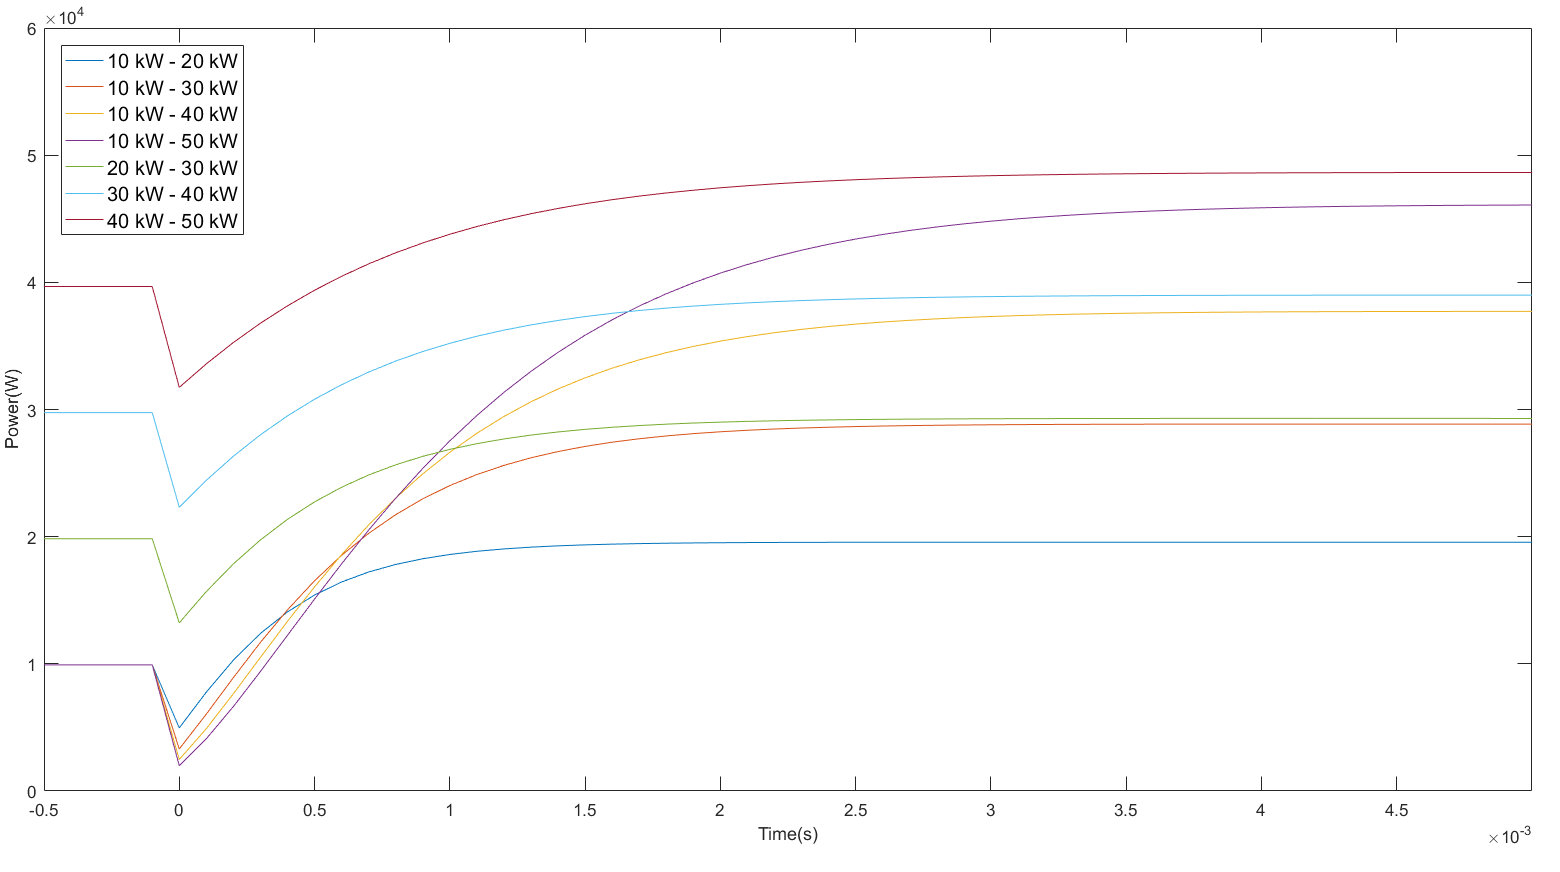
\includegraphics[width=1.1\textwidth]{rapport/billeder/gensetdata2}
 % \caption{\fxnote{yeah i know the figure need scaling and other stuff :)}}
 % \label{fig:gensetdata2}
 % \end{figure}

\begin{figure}[H]
\centering
% This file was created by matlab2tikz.
%
%The latest updates can be retrieved from
%  http://www.mathworks.com/matlabcentral/fileexchange/22022-matlab2tikz-matlab2tikz
%where you can also make suggestions and rate matlab2tikz.
%
\definecolor{mycolor1}{rgb}{0.00000,0.44700,0.74100}%
\definecolor{mycolor2}{rgb}{0.85000,0.32500,0.09800}%
\definecolor{mycolor3}{rgb}{0.92900,0.69400,0.12500}%
\definecolor{mycolor4}{rgb}{0.49400,0.18400,0.55600}%
\definecolor{mycolor5}{rgb}{0.46600,0.67400,0.18800}%
\definecolor{mycolor6}{rgb}{0.30100,0.74500,0.93300}%
\definecolor{mycolor7}{rgb}{0.63500,0.07800,0.18400}%
%
\begin{tikzpicture}

\begin{axis}[%
width=4.521in,
height=3.527in,
at={(0.758in,0.519in)},
scale only axis,
xmin=-0.2,
xmax=2.4,
xlabel={Time[s]},
xmajorgrids,
ymin=0,
ymax=60,
ylabel={Power[kW]},
ymajorgrids,
axis background/.style={fill=white},
legend style={at={(0.97,0.03)},anchor=south east,legend cell align=left,align=left,draw=black},
y filter/.code={\pgfmathparse{#1/1000}\pgfmathresult}
]
\addplot [color=mycolor1,solid,line width=2.0pt]
  table[row sep=crcr]{%
-0.2	9919\\
-0.19	9919\\
-0.18	9919\\
-0.17	9919\\
-0.16	9919\\
-0.15	9919\\
-0.14	9919\\
-0.13	9919\\
-0.12	9919\\
-0.11	9919\\
-0.1	9919\\
-0.09	9919\\
-0.08	9919\\
-0.07	9919\\
-0.06	9919\\
-0.05	9919\\
-0.04	9919\\
-0.03	9919\\
-0.02	9919\\
-0.01	9919\\
0	4959\\
0.01	1.953e+04\\
0.02	1.948e+04\\
0.03	1.943e+04\\
0.04	1.939e+04\\
0.05	1.935e+04\\
0.06	1.931e+04\\
0.07	1.928e+04\\
0.08	1.925e+04\\
0.09	1.924e+04\\
0.1	1.922e+04\\
0.11	1.922e+04\\
0.12	1.922e+04\\
0.13	1.922e+04\\
0.14	1.923e+04\\
0.15	1.925e+04\\
0.16	1.928e+04\\
0.17	1.93e+04\\
0.18	1.934e+04\\
0.19	1.938e+04\\
0.2	1.942e+04\\
0.21	1.946e+04\\
0.22	1.951e+04\\
0.23	1.956e+04\\
0.24	1.961e+04\\
0.25	1.966e+04\\
0.26	1.972e+04\\
0.27	1.977e+04\\
0.28	1.983e+04\\
0.29	1.988e+04\\
0.3	1.993e+04\\
0.31	1.998e+04\\
0.32	2.003e+04\\
0.33	2.008e+04\\
0.34	2.012e+04\\
0.35	2.017e+04\\
0.36	2.02e+04\\
0.37	2.024e+04\\
0.38	2.027e+04\\
0.39	2.03e+04\\
0.4	2.033e+04\\
0.41	2.035e+04\\
0.42	2.037e+04\\
0.43	2.039e+04\\
0.44	2.04e+04\\
0.45	2.041e+04\\
0.46	2.041e+04\\
0.47	2.042e+04\\
0.48	2.042e+04\\
0.49	2.041e+04\\
0.5	2.041e+04\\
0.51	2.04e+04\\
0.52	2.039e+04\\
0.53	2.038e+04\\
0.54	2.036e+04\\
0.55	2.035e+04\\
0.56	2.033e+04\\
0.57	2.031e+04\\
0.58	2.029e+04\\
0.59	2.027e+04\\
0.6	2.025e+04\\
0.61	2.022e+04\\
0.62	2.02e+04\\
0.63	2.018e+04\\
0.64	2.015e+04\\
0.65	2.013e+04\\
0.66	2.01e+04\\
0.67	2.008e+04\\
0.68	2.006e+04\\
0.69	2.003e+04\\
0.7	2.001e+04\\
0.71	1.999e+04\\
0.72	1.997e+04\\
0.73	1.995e+04\\
0.74	1.993e+04\\
0.75	1.991e+04\\
0.76	1.989e+04\\
0.77	1.988e+04\\
0.78	1.986e+04\\
0.79	1.985e+04\\
0.8	1.983e+04\\
0.81	1.982e+04\\
0.82	1.981e+04\\
0.83	1.98e+04\\
0.84	1.979e+04\\
0.85	1.978e+04\\
0.86	1.977e+04\\
0.87	1.976e+04\\
0.88	1.975e+04\\
0.89	1.975e+04\\
0.9	1.974e+04\\
0.91	1.974e+04\\
0.92	1.973e+04\\
0.93	1.973e+04\\
0.94	1.973e+04\\
0.95	1.972e+04\\
0.96	1.972e+04\\
0.97	1.972e+04\\
0.98	1.972e+04\\
0.99	1.972e+04\\
1	1.972e+04\\
1.01	1.972e+04\\
1.02	1.972e+04\\
1.03	1.972e+04\\
1.04	1.972e+04\\
1.05	1.972e+04\\
1.06	1.972e+04\\
1.07	1.972e+04\\
1.08	1.972e+04\\
1.09	1.973e+04\\
1.1	1.973e+04\\
1.11	1.973e+04\\
1.12	1.973e+04\\
1.13	1.973e+04\\
1.14	1.974e+04\\
1.15	1.974e+04\\
1.16	1.974e+04\\
1.17	1.974e+04\\
1.18	1.974e+04\\
1.19	1.975e+04\\
1.2	1.975e+04\\
1.21	1.975e+04\\
1.22	1.975e+04\\
1.23	1.975e+04\\
1.24	1.976e+04\\
1.25	1.976e+04\\
1.26	1.976e+04\\
1.27	1.976e+04\\
1.28	1.976e+04\\
1.29	1.976e+04\\
1.3	1.977e+04\\
1.31	1.977e+04\\
1.32	1.977e+04\\
1.33	1.977e+04\\
1.34	1.977e+04\\
1.35	1.977e+04\\
1.36	1.978e+04\\
1.37	1.978e+04\\
1.38	1.978e+04\\
1.39	1.978e+04\\
1.4	1.978e+04\\
1.41	1.978e+04\\
1.42	1.979e+04\\
1.43	1.979e+04\\
1.44	1.979e+04\\
1.45	1.979e+04\\
1.46	1.979e+04\\
1.47	1.979e+04\\
1.48	1.98e+04\\
1.49	1.98e+04\\
1.5	1.98e+04\\
1.51	1.98e+04\\
1.52	1.98e+04\\
1.53	1.98e+04\\
1.54	1.98e+04\\
1.55	1.981e+04\\
1.56	1.981e+04\\
1.57	1.981e+04\\
1.58	1.981e+04\\
1.59	1.981e+04\\
1.6	1.981e+04\\
1.61	1.981e+04\\
1.62	1.982e+04\\
1.63	1.982e+04\\
1.64	1.982e+04\\
1.65	1.982e+04\\
1.66	1.982e+04\\
1.67	1.982e+04\\
1.68	1.982e+04\\
1.69	1.982e+04\\
1.7	1.983e+04\\
1.71	1.983e+04\\
1.72	1.983e+04\\
1.73	1.983e+04\\
1.74	1.983e+04\\
1.75	1.983e+04\\
1.76	1.983e+04\\
1.77	1.983e+04\\
1.78	1.983e+04\\
1.79	1.983e+04\\
1.8	1.983e+04\\
1.81	1.984e+04\\
1.82	1.984e+04\\
1.83	1.984e+04\\
1.84	1.984e+04\\
1.85	1.984e+04\\
1.86	1.984e+04\\
1.87	1.984e+04\\
1.88	1.984e+04\\
1.89	1.984e+04\\
1.9	1.984e+04\\
1.91	1.984e+04\\
1.92	1.984e+04\\
1.93	1.984e+04\\
1.94	1.984e+04\\
1.95	1.984e+04\\
1.96	1.984e+04\\
1.97	1.984e+04\\
1.98	1.984e+04\\
1.99	1.984e+04\\
2	1.984e+04\\
2.01	1.984e+04\\
2.02	1.984e+04\\
2.03	1.984e+04\\
2.04	1.984e+04\\
2.05	1.984e+04\\
2.06	1.984e+04\\
2.07	1.984e+04\\
2.08	1.984e+04\\
2.09	1.984e+04\\
2.1	1.984e+04\\
2.11	1.984e+04\\
2.12	1.984e+04\\
2.13	1.984e+04\\
2.14	1.984e+04\\
2.15	1.984e+04\\
2.16	1.984e+04\\
2.17	1.984e+04\\
2.18	1.984e+04\\
2.19	1.984e+04\\
2.2	1.984e+04\\
2.21	1.984e+04\\
2.22	1.984e+04\\
2.23	1.984e+04\\
2.24	1.984e+04\\
2.25	1.984e+04\\
2.26	1.984e+04\\
2.27	1.984e+04\\
2.28	1.984e+04\\
2.29	1.984e+04\\
2.3	1.984e+04\\
2.31	1.984e+04\\
2.32	1.984e+04\\
2.33	1.984e+04\\
2.34	1.984e+04\\
2.35	1.984e+04\\
2.36	1.984e+04\\
2.37	1.984e+04\\
2.38	1.984e+04\\
2.39	1.984e+04\\
2.4	1.984e+04\\
2.4	1.984e+04\\
};
\addlegendentry{10 kW - 20 kW};

\addplot [color=mycolor2,solid,line width=2.0pt]
  table[row sep=crcr]{%
-0.2	9919\\
-0.19	9919\\
-0.18	9919\\
-0.17	9919\\
-0.16	9919\\
-0.15	9919\\
-0.14	9919\\
-0.13	9919\\
-0.12	9919\\
-0.11	9919\\
-0.1	9919\\
-0.09	9919\\
-0.08	9919\\
-0.07	9919\\
-0.06	9919\\
-0.05	9919\\
-0.04	9919\\
-0.03	9919\\
-0.02	9919\\
-0.01	9919\\
0	3306\\
0.01	2.877e+04\\
0.02	2.862e+04\\
0.03	2.848e+04\\
0.04	2.836e+04\\
0.05	2.824e+04\\
0.06	2.814e+04\\
0.07	2.806e+04\\
0.08	2.799e+04\\
0.09	2.794e+04\\
0.1	2.791e+04\\
0.11	2.789e+04\\
0.12	2.789e+04\\
0.13	2.791e+04\\
0.14	2.794e+04\\
0.15	2.799e+04\\
0.16	2.805e+04\\
0.17	2.813e+04\\
0.18	2.823e+04\\
0.19	2.833e+04\\
0.2	2.845e+04\\
0.21	2.858e+04\\
0.22	2.871e+04\\
0.23	2.885e+04\\
0.24	2.9e+04\\
0.25	2.916e+04\\
0.26	2.931e+04\\
0.27	2.947e+04\\
0.28	2.963e+04\\
0.29	2.978e+04\\
0.3	2.994e+04\\
0.31	3.009e+04\\
0.32	3.023e+04\\
0.33	3.038e+04\\
0.34	3.051e+04\\
0.35	3.064e+04\\
0.36	3.076e+04\\
0.37	3.087e+04\\
0.38	3.097e+04\\
0.39	3.106e+04\\
0.4	3.115e+04\\
0.41	3.122e+04\\
0.42	3.129e+04\\
0.43	3.134e+04\\
0.44	3.139e+04\\
0.45	3.142e+04\\
0.46	3.145e+04\\
0.47	3.146e+04\\
0.48	3.147e+04\\
0.49	3.147e+04\\
0.5	3.146e+04\\
0.51	3.145e+04\\
0.52	3.142e+04\\
0.53	3.139e+04\\
0.54	3.136e+04\\
0.55	3.132e+04\\
0.56	3.127e+04\\
0.57	3.122e+04\\
0.58	3.117e+04\\
0.59	3.112e+04\\
0.6	3.106e+04\\
0.61	3.099e+04\\
0.62	3.093e+04\\
0.63	3.087e+04\\
0.64	3.08e+04\\
0.65	3.073e+04\\
0.66	3.067e+04\\
0.67	3.06e+04\\
0.68	3.054e+04\\
0.69	3.047e+04\\
0.7	3.041e+04\\
0.71	3.034e+04\\
0.72	3.028e+04\\
0.73	3.022e+04\\
0.74	3.016e+04\\
0.75	3.011e+04\\
0.76	3.005e+04\\
0.77	3e+04\\
0.78	2.995e+04\\
0.79	2.99e+04\\
0.8	2.986e+04\\
0.81	2.982e+04\\
0.82	2.978e+04\\
0.83	2.974e+04\\
0.84	2.97e+04\\
0.85	2.967e+04\\
0.86	2.964e+04\\
0.87	2.961e+04\\
0.88	2.958e+04\\
0.89	2.955e+04\\
0.9	2.953e+04\\
0.91	2.951e+04\\
0.92	2.949e+04\\
0.93	2.947e+04\\
0.94	2.946e+04\\
0.95	2.944e+04\\
0.96	2.943e+04\\
0.97	2.942e+04\\
0.98	2.941e+04\\
0.99	2.94e+04\\
1	2.94e+04\\
1.01	2.939e+04\\
1.02	2.939e+04\\
1.03	2.938e+04\\
1.04	2.938e+04\\
1.05	2.938e+04\\
1.06	2.938e+04\\
1.07	2.938e+04\\
1.08	2.938e+04\\
1.09	2.938e+04\\
1.1	2.938e+04\\
1.11	2.938e+04\\
1.12	2.938e+04\\
1.13	2.939e+04\\
1.14	2.939e+04\\
1.15	2.939e+04\\
1.16	2.94e+04\\
1.17	2.94e+04\\
1.18	2.941e+04\\
1.19	2.941e+04\\
1.2	2.942e+04\\
1.21	2.942e+04\\
1.22	2.943e+04\\
1.23	2.944e+04\\
1.24	2.944e+04\\
1.25	2.945e+04\\
1.26	2.946e+04\\
1.27	2.946e+04\\
1.28	2.947e+04\\
1.29	2.948e+04\\
1.3	2.948e+04\\
1.31	2.949e+04\\
1.32	2.95e+04\\
1.33	2.95e+04\\
1.34	2.951e+04\\
1.35	2.952e+04\\
1.36	2.952e+04\\
1.37	2.953e+04\\
1.38	2.954e+04\\
1.39	2.954e+04\\
1.4	2.955e+04\\
1.41	2.956e+04\\
1.42	2.956e+04\\
1.43	2.957e+04\\
1.44	2.958e+04\\
1.45	2.959e+04\\
1.46	2.959e+04\\
1.47	2.96e+04\\
1.48	2.961e+04\\
1.49	2.961e+04\\
1.5	2.962e+04\\
1.51	2.962e+04\\
1.52	2.963e+04\\
1.53	2.964e+04\\
1.54	2.964e+04\\
1.55	2.965e+04\\
1.56	2.966e+04\\
1.57	2.966e+04\\
1.58	2.967e+04\\
1.59	2.967e+04\\
1.6	2.968e+04\\
1.61	2.968e+04\\
1.62	2.969e+04\\
1.63	2.969e+04\\
1.64	2.97e+04\\
1.65	2.97e+04\\
1.66	2.971e+04\\
1.67	2.971e+04\\
1.68	2.972e+04\\
1.69	2.972e+04\\
1.7	2.973e+04\\
1.71	2.973e+04\\
1.72	2.973e+04\\
1.73	2.974e+04\\
1.74	2.974e+04\\
1.75	2.974e+04\\
1.76	2.975e+04\\
1.77	2.975e+04\\
1.78	2.975e+04\\
1.79	2.976e+04\\
1.8	2.976e+04\\
1.81	2.976e+04\\
1.82	2.976e+04\\
1.83	2.976e+04\\
1.84	2.977e+04\\
1.85	2.977e+04\\
1.86	2.977e+04\\
1.87	2.977e+04\\
1.88	2.977e+04\\
1.89	2.977e+04\\
1.9	2.978e+04\\
1.91	2.978e+04\\
1.92	2.978e+04\\
1.93	2.978e+04\\
1.94	2.978e+04\\
1.95	2.978e+04\\
1.96	2.978e+04\\
1.97	2.978e+04\\
1.98	2.978e+04\\
1.99	2.978e+04\\
2	2.978e+04\\
2.01	2.978e+04\\
2.02	2.978e+04\\
2.03	2.978e+04\\
2.04	2.978e+04\\
2.05	2.978e+04\\
2.06	2.978e+04\\
2.07	2.978e+04\\
2.08	2.978e+04\\
2.09	2.978e+04\\
2.1	2.978e+04\\
2.11	2.978e+04\\
2.12	2.978e+04\\
2.13	2.978e+04\\
2.14	2.978e+04\\
2.15	2.978e+04\\
2.16	2.978e+04\\
2.17	2.978e+04\\
2.18	2.978e+04\\
2.19	2.978e+04\\
2.2	2.978e+04\\
2.21	2.978e+04\\
2.22	2.978e+04\\
2.23	2.977e+04\\
2.24	2.977e+04\\
2.25	2.977e+04\\
2.26	2.977e+04\\
2.27	2.977e+04\\
2.28	2.977e+04\\
2.29	2.977e+04\\
2.3	2.977e+04\\
2.31	2.977e+04\\
2.32	2.977e+04\\
2.33	2.977e+04\\
2.34	2.977e+04\\
2.35	2.977e+04\\
2.36	2.977e+04\\
2.37	2.976e+04\\
2.38	2.976e+04\\
2.39	2.976e+04\\
2.4	2.976e+04\\
2.4	2.976e+04\\
};
\addlegendentry{10 kW - 30 kW};

\addplot [color=mycolor3,solid,line width=2.0pt]
  table[row sep=crcr]{%
-0.2	9919\\
-0.19	9919\\
-0.18	9919\\
-0.17	9919\\
-0.16	9919\\
-0.15	9919\\
-0.14	9919\\
-0.13	9919\\
-0.12	9919\\
-0.11	9919\\
-0.1	9919\\
-0.09	9919\\
-0.08	9919\\
-0.07	9919\\
-0.06	9919\\
-0.05	9919\\
-0.04	9919\\
-0.03	9919\\
-0.02	9919\\
-0.01	9919\\
0	2480\\
0.01	3.757e+04\\
0.02	3.728e+04\\
0.03	3.702e+04\\
0.04	3.678e+04\\
0.05	3.658e+04\\
0.06	3.64e+04\\
0.07	3.625e+04\\
0.08	3.612e+04\\
0.09	3.603e+04\\
0.1	3.596e+04\\
0.11	3.593e+04\\
0.12	3.593e+04\\
0.13	3.596e+04\\
0.14	3.602e+04\\
0.15	3.611e+04\\
0.16	3.623e+04\\
0.17	3.638e+04\\
0.18	3.655e+04\\
0.19	3.675e+04\\
0.2	3.697e+04\\
0.21	3.721e+04\\
0.22	3.746e+04\\
0.23	3.773e+04\\
0.24	3.802e+04\\
0.25	3.831e+04\\
0.26	3.861e+04\\
0.27	3.891e+04\\
0.28	3.922e+04\\
0.29	3.952e+04\\
0.3	3.982e+04\\
0.31	4.012e+04\\
0.32	4.041e+04\\
0.33	4.069e+04\\
0.34	4.096e+04\\
0.35	4.121e+04\\
0.36	4.146e+04\\
0.37	4.168e+04\\
0.38	4.189e+04\\
0.39	4.209e+04\\
0.4	4.226e+04\\
0.41	4.242e+04\\
0.42	4.256e+04\\
0.43	4.268e+04\\
0.44	4.279e+04\\
0.45	4.287e+04\\
0.46	4.294e+04\\
0.47	4.299e+04\\
0.48	4.302e+04\\
0.49	4.304e+04\\
0.5	4.304e+04\\
0.51	4.303e+04\\
0.52	4.3e+04\\
0.53	4.296e+04\\
0.54	4.291e+04\\
0.55	4.285e+04\\
0.56	4.278e+04\\
0.57	4.27e+04\\
0.58	4.261e+04\\
0.59	4.252e+04\\
0.6	4.241e+04\\
0.61	4.231e+04\\
0.62	4.22e+04\\
0.63	4.208e+04\\
0.64	4.196e+04\\
0.65	4.184e+04\\
0.66	4.172e+04\\
0.67	4.16e+04\\
0.68	4.148e+04\\
0.69	4.135e+04\\
0.7	4.123e+04\\
0.71	4.111e+04\\
0.72	4.1e+04\\
0.73	4.088e+04\\
0.74	4.076e+04\\
0.75	4.065e+04\\
0.76	4.055e+04\\
0.77	4.044e+04\\
0.78	4.034e+04\\
0.79	4.024e+04\\
0.8	4.014e+04\\
0.81	4.005e+04\\
0.82	3.996e+04\\
0.83	3.988e+04\\
0.84	3.98e+04\\
0.85	3.972e+04\\
0.86	3.965e+04\\
0.87	3.958e+04\\
0.88	3.952e+04\\
0.89	3.946e+04\\
0.9	3.94e+04\\
0.91	3.934e+04\\
0.92	3.929e+04\\
0.93	3.925e+04\\
0.94	3.92e+04\\
0.95	3.916e+04\\
0.96	3.912e+04\\
0.97	3.909e+04\\
0.98	3.906e+04\\
0.99	3.903e+04\\
1	3.9e+04\\
1.01	3.898e+04\\
1.02	3.895e+04\\
1.03	3.893e+04\\
1.04	3.892e+04\\
1.05	3.89e+04\\
1.06	3.889e+04\\
1.07	3.888e+04\\
1.08	3.887e+04\\
1.09	3.886e+04\\
1.1	3.886e+04\\
1.11	3.885e+04\\
1.12	3.885e+04\\
1.13	3.885e+04\\
1.14	3.885e+04\\
1.15	3.885e+04\\
1.16	3.886e+04\\
1.17	3.886e+04\\
1.18	3.887e+04\\
1.19	3.887e+04\\
1.2	3.888e+04\\
1.21	3.889e+04\\
1.22	3.89e+04\\
1.23	3.891e+04\\
1.24	3.892e+04\\
1.25	3.893e+04\\
1.26	3.894e+04\\
1.27	3.896e+04\\
1.28	3.897e+04\\
1.29	3.898e+04\\
1.3	3.9e+04\\
1.31	3.901e+04\\
1.32	3.903e+04\\
1.33	3.904e+04\\
1.34	3.906e+04\\
1.35	3.907e+04\\
1.36	3.909e+04\\
1.37	3.911e+04\\
1.38	3.913e+04\\
1.39	3.914e+04\\
1.4	3.916e+04\\
1.41	3.918e+04\\
1.42	3.919e+04\\
1.43	3.921e+04\\
1.44	3.923e+04\\
1.45	3.925e+04\\
1.46	3.926e+04\\
1.47	3.928e+04\\
1.48	3.93e+04\\
1.49	3.931e+04\\
1.5	3.933e+04\\
1.51	3.935e+04\\
1.52	3.936e+04\\
1.53	3.938e+04\\
1.54	3.94e+04\\
1.55	3.941e+04\\
1.56	3.943e+04\\
1.57	3.944e+04\\
1.58	3.946e+04\\
1.59	3.947e+04\\
1.6	3.949e+04\\
1.61	3.95e+04\\
1.62	3.951e+04\\
1.63	3.953e+04\\
1.64	3.954e+04\\
1.65	3.955e+04\\
1.66	3.957e+04\\
1.67	3.958e+04\\
1.68	3.959e+04\\
1.69	3.96e+04\\
1.7	3.961e+04\\
1.71	3.962e+04\\
1.72	3.963e+04\\
1.73	3.964e+04\\
1.74	3.965e+04\\
1.75	3.966e+04\\
1.76	3.967e+04\\
1.77	3.968e+04\\
1.78	3.968e+04\\
1.79	3.969e+04\\
1.8	3.97e+04\\
1.81	3.97e+04\\
1.82	3.971e+04\\
1.83	3.971e+04\\
1.84	3.972e+04\\
1.85	3.972e+04\\
1.86	3.973e+04\\
1.87	3.973e+04\\
1.88	3.974e+04\\
1.89	3.974e+04\\
1.9	3.974e+04\\
1.91	3.975e+04\\
1.92	3.975e+04\\
1.93	3.975e+04\\
1.94	3.975e+04\\
1.95	3.976e+04\\
1.96	3.976e+04\\
1.97	3.976e+04\\
1.98	3.976e+04\\
1.99	3.976e+04\\
2	3.976e+04\\
2.01	3.976e+04\\
2.02	3.976e+04\\
2.03	3.976e+04\\
2.04	3.976e+04\\
2.05	3.976e+04\\
2.06	3.976e+04\\
2.07	3.976e+04\\
2.08	3.976e+04\\
2.09	3.976e+04\\
2.1	3.976e+04\\
2.11	3.976e+04\\
2.12	3.975e+04\\
2.13	3.975e+04\\
2.14	3.975e+04\\
2.15	3.975e+04\\
2.16	3.975e+04\\
2.17	3.975e+04\\
2.18	3.974e+04\\
2.19	3.974e+04\\
2.2	3.974e+04\\
2.21	3.974e+04\\
2.22	3.974e+04\\
2.23	3.973e+04\\
2.24	3.973e+04\\
2.25	3.973e+04\\
2.26	3.973e+04\\
2.27	3.972e+04\\
2.28	3.972e+04\\
2.29	3.972e+04\\
2.3	3.972e+04\\
2.31	3.972e+04\\
2.32	3.971e+04\\
2.33	3.971e+04\\
2.34	3.971e+04\\
2.35	3.971e+04\\
2.36	3.97e+04\\
2.37	3.97e+04\\
2.38	3.97e+04\\
2.39	3.97e+04\\
2.4	3.97e+04\\
2.4	3.97e+04\\
};
\addlegendentry{10 kW - 40 kW};

\addplot [color=mycolor4,solid,line width=2.0pt]
  table[row sep=crcr]{%
-0.2	9919\\
-0.19	9919\\
-0.18	9919\\
-0.17	9919\\
-0.16	9919\\
-0.15	9919\\
-0.14	9919\\
-0.13	9919\\
-0.12	9919\\
-0.11	9919\\
-0.1	9919\\
-0.09	9919\\
-0.08	9919\\
-0.07	9919\\
-0.06	9919\\
-0.05	9919\\
-0.04	9919\\
-0.03	9919\\
-0.02	9919\\
-0.01	9919\\
0	1984\\
0.01	4.59e+04\\
0.02	4.542e+04\\
0.03	4.5e+04\\
0.04	4.464e+04\\
0.05	4.432e+04\\
0.06	4.405e+04\\
0.07	4.382e+04\\
0.08	4.363e+04\\
0.09	4.348e+04\\
0.1	4.338e+04\\
0.11	4.333e+04\\
0.12	4.332e+04\\
0.13	4.337e+04\\
0.14	4.346e+04\\
0.15	4.36e+04\\
0.16	4.378e+04\\
0.17	4.401e+04\\
0.18	4.428e+04\\
0.19	4.458e+04\\
0.2	4.493e+04\\
0.21	4.53e+04\\
0.22	4.57e+04\\
0.23	4.613e+04\\
0.24	4.658e+04\\
0.25	4.704e+04\\
0.26	4.752e+04\\
0.27	4.8e+04\\
0.28	4.849e+04\\
0.29	4.898e+04\\
0.3	4.947e+04\\
0.31	4.995e+04\\
0.32	5.042e+04\\
0.33	5.088e+04\\
0.34	5.133e+04\\
0.35	5.175e+04\\
0.36	5.216e+04\\
0.37	5.254e+04\\
0.38	5.29e+04\\
0.39	5.323e+04\\
0.4	5.354e+04\\
0.41	5.382e+04\\
0.42	5.407e+04\\
0.43	5.429e+04\\
0.44	5.448e+04\\
0.45	5.465e+04\\
0.46	5.478e+04\\
0.47	5.49e+04\\
0.48	5.498e+04\\
0.49	5.504e+04\\
0.5	5.507e+04\\
0.51	5.508e+04\\
0.52	5.507e+04\\
0.53	5.504e+04\\
0.54	5.499e+04\\
0.55	5.492e+04\\
0.56	5.483e+04\\
0.57	5.473e+04\\
0.58	5.462e+04\\
0.59	5.449e+04\\
0.6	5.435e+04\\
0.61	5.421e+04\\
0.62	5.405e+04\\
0.63	5.388e+04\\
0.64	5.371e+04\\
0.65	5.354e+04\\
0.66	5.336e+04\\
0.67	5.318e+04\\
0.68	5.299e+04\\
0.69	5.281e+04\\
0.7	5.262e+04\\
0.71	5.243e+04\\
0.72	5.225e+04\\
0.73	5.206e+04\\
0.74	5.188e+04\\
0.75	5.17e+04\\
0.76	5.153e+04\\
0.77	5.135e+04\\
0.78	5.118e+04\\
0.79	5.101e+04\\
0.8	5.085e+04\\
0.81	5.069e+04\\
0.82	5.054e+04\\
0.83	5.039e+04\\
0.84	5.025e+04\\
0.85	5.011e+04\\
0.86	4.997e+04\\
0.87	4.985e+04\\
0.88	4.972e+04\\
0.89	4.96e+04\\
0.9	4.949e+04\\
0.91	4.938e+04\\
0.92	4.928e+04\\
0.93	4.918e+04\\
0.94	4.908e+04\\
0.95	4.9e+04\\
0.96	4.891e+04\\
0.97	4.883e+04\\
0.98	4.876e+04\\
0.99	4.869e+04\\
1	4.862e+04\\
1.01	4.856e+04\\
1.02	4.851e+04\\
1.03	4.845e+04\\
1.04	4.841e+04\\
1.05	4.836e+04\\
1.06	4.832e+04\\
1.07	4.829e+04\\
1.08	4.825e+04\\
1.09	4.822e+04\\
1.1	4.82e+04\\
1.11	4.818e+04\\
1.12	4.816e+04\\
1.13	4.814e+04\\
1.14	4.813e+04\\
1.15	4.812e+04\\
1.16	4.811e+04\\
1.17	4.811e+04\\
1.18	4.811e+04\\
1.19	4.811e+04\\
1.2	4.811e+04\\
1.21	4.812e+04\\
1.22	4.812e+04\\
1.23	4.813e+04\\
1.24	4.814e+04\\
1.25	4.816e+04\\
1.26	4.817e+04\\
1.27	4.819e+04\\
1.28	4.821e+04\\
1.29	4.823e+04\\
1.3	4.825e+04\\
1.31	4.828e+04\\
1.32	4.83e+04\\
1.33	4.833e+04\\
1.34	4.835e+04\\
1.35	4.838e+04\\
1.36	4.841e+04\\
1.37	4.844e+04\\
1.38	4.847e+04\\
1.39	4.85e+04\\
1.4	4.853e+04\\
1.41	4.857e+04\\
1.42	4.86e+04\\
1.43	4.863e+04\\
1.44	4.866e+04\\
1.45	4.87e+04\\
1.46	4.873e+04\\
1.47	4.876e+04\\
1.48	4.88e+04\\
1.49	4.883e+04\\
1.5	4.887e+04\\
1.51	4.89e+04\\
1.52	4.893e+04\\
1.53	4.897e+04\\
1.54	4.9e+04\\
1.55	4.903e+04\\
1.56	4.906e+04\\
1.57	4.909e+04\\
1.58	4.913e+04\\
1.59	4.916e+04\\
1.6	4.919e+04\\
1.61	4.922e+04\\
1.62	4.925e+04\\
1.63	4.927e+04\\
1.64	4.93e+04\\
1.65	4.933e+04\\
1.66	4.935e+04\\
1.67	4.938e+04\\
1.68	4.941e+04\\
1.69	4.943e+04\\
1.7	4.945e+04\\
1.71	4.948e+04\\
1.72	4.95e+04\\
1.73	4.952e+04\\
1.74	4.954e+04\\
1.75	4.956e+04\\
1.76	4.958e+04\\
1.77	4.959e+04\\
1.78	4.961e+04\\
1.79	4.963e+04\\
1.8	4.964e+04\\
1.81	4.966e+04\\
1.82	4.967e+04\\
1.83	4.968e+04\\
1.84	4.97e+04\\
1.85	4.971e+04\\
1.86	4.972e+04\\
1.87	4.973e+04\\
1.88	4.974e+04\\
1.89	4.975e+04\\
1.9	4.976e+04\\
1.91	4.976e+04\\
1.92	4.977e+04\\
1.93	4.978e+04\\
1.94	4.978e+04\\
1.95	4.979e+04\\
1.96	4.979e+04\\
1.97	4.979e+04\\
1.98	4.98e+04\\
1.99	4.98e+04\\
2	4.98e+04\\
2.01	4.98e+04\\
2.02	4.98e+04\\
2.03	4.98e+04\\
2.04	4.98e+04\\
2.05	4.98e+04\\
2.06	4.98e+04\\
2.07	4.98e+04\\
2.08	4.98e+04\\
2.09	4.98e+04\\
2.1	4.979e+04\\
2.11	4.979e+04\\
2.12	4.979e+04\\
2.13	4.979e+04\\
2.14	4.978e+04\\
2.15	4.978e+04\\
2.16	4.977e+04\\
2.17	4.977e+04\\
2.18	4.977e+04\\
2.19	4.976e+04\\
2.2	4.976e+04\\
2.21	4.975e+04\\
2.22	4.975e+04\\
2.23	4.974e+04\\
2.24	4.974e+04\\
2.25	4.973e+04\\
2.26	4.973e+04\\
2.27	4.972e+04\\
2.28	4.972e+04\\
2.29	4.971e+04\\
2.3	4.971e+04\\
2.31	4.97e+04\\
2.32	4.969e+04\\
2.33	4.969e+04\\
2.34	4.968e+04\\
2.35	4.968e+04\\
2.36	4.967e+04\\
2.37	4.967e+04\\
2.38	4.966e+04\\
2.39	4.966e+04\\
2.4	4.965e+04\\
2.4	4.965e+04\\
};
\addlegendentry{10 kW - 50 kW};

\addplot [color=mycolor5,solid,line width=2.0pt]
  table[row sep=crcr]{%
-0.2	1.984e+04\\
-0.19	1.984e+04\\
-0.18	1.984e+04\\
-0.17	1.984e+04\\
-0.16	1.984e+04\\
-0.15	1.984e+04\\
-0.14	1.984e+04\\
-0.13	1.984e+04\\
-0.12	1.984e+04\\
-0.11	1.984e+04\\
-0.1	1.984e+04\\
-0.09	1.984e+04\\
-0.08	1.984e+04\\
-0.07	1.984e+04\\
-0.06	1.984e+04\\
-0.05	1.984e+04\\
-0.04	1.984e+04\\
-0.03	1.984e+04\\
-0.02	1.984e+04\\
-0.01	1.984e+04\\
0	1.322e+04\\
0.01	2.926e+04\\
0.02	2.918e+04\\
0.03	2.911e+04\\
0.04	2.904e+04\\
0.05	2.898e+04\\
0.06	2.893e+04\\
0.07	2.888e+04\\
0.08	2.885e+04\\
0.09	2.882e+04\\
0.1	2.88e+04\\
0.11	2.88e+04\\
0.12	2.88e+04\\
0.13	2.881e+04\\
0.14	2.882e+04\\
0.15	2.885e+04\\
0.16	2.889e+04\\
0.17	2.893e+04\\
0.18	2.898e+04\\
0.19	2.903e+04\\
0.2	2.909e+04\\
0.21	2.916e+04\\
0.22	2.923e+04\\
0.23	2.93e+04\\
0.24	2.937e+04\\
0.25	2.945e+04\\
0.26	2.953e+04\\
0.27	2.961e+04\\
0.28	2.969e+04\\
0.29	2.976e+04\\
0.3	2.984e+04\\
0.31	2.992e+04\\
0.32	2.999e+04\\
0.33	3.006e+04\\
0.34	3.012e+04\\
0.35	3.019e+04\\
0.36	3.024e+04\\
0.37	3.03e+04\\
0.38	3.035e+04\\
0.39	3.039e+04\\
0.4	3.043e+04\\
0.41	3.047e+04\\
0.42	3.05e+04\\
0.43	3.053e+04\\
0.44	3.055e+04\\
0.45	3.057e+04\\
0.46	3.058e+04\\
0.47	3.059e+04\\
0.48	3.059e+04\\
0.49	3.059e+04\\
0.5	3.058e+04\\
0.51	3.058e+04\\
0.52	3.057e+04\\
0.53	3.055e+04\\
0.54	3.054e+04\\
0.55	3.052e+04\\
0.56	3.049e+04\\
0.57	3.047e+04\\
0.58	3.044e+04\\
0.59	3.042e+04\\
0.6	3.039e+04\\
0.61	3.036e+04\\
0.62	3.033e+04\\
0.63	3.03e+04\\
0.64	3.026e+04\\
0.65	3.023e+04\\
0.66	3.02e+04\\
0.67	3.017e+04\\
0.68	3.013e+04\\
0.69	3.01e+04\\
0.7	3.007e+04\\
0.71	3.004e+04\\
0.72	3.001e+04\\
0.73	2.998e+04\\
0.74	2.995e+04\\
0.75	2.993e+04\\
0.76	2.99e+04\\
0.77	2.987e+04\\
0.78	2.985e+04\\
0.79	2.983e+04\\
0.8	2.98e+04\\
0.81	2.978e+04\\
0.82	2.976e+04\\
0.83	2.975e+04\\
0.84	2.973e+04\\
0.85	2.971e+04\\
0.86	2.97e+04\\
0.87	2.968e+04\\
0.88	2.967e+04\\
0.89	2.966e+04\\
0.9	2.965e+04\\
0.91	2.964e+04\\
0.92	2.963e+04\\
0.93	2.962e+04\\
0.94	2.961e+04\\
0.95	2.96e+04\\
0.96	2.96e+04\\
0.97	2.959e+04\\
0.98	2.959e+04\\
0.99	2.958e+04\\
1	2.958e+04\\
1.01	2.958e+04\\
1.02	2.958e+04\\
1.03	2.957e+04\\
1.04	2.957e+04\\
1.05	2.957e+04\\
1.06	2.957e+04\\
1.07	2.957e+04\\
1.08	2.957e+04\\
1.09	2.957e+04\\
1.1	2.957e+04\\
1.11	2.958e+04\\
1.12	2.958e+04\\
1.13	2.958e+04\\
1.14	2.958e+04\\
1.15	2.958e+04\\
1.16	2.958e+04\\
1.17	2.959e+04\\
1.18	2.959e+04\\
1.19	2.959e+04\\
1.2	2.959e+04\\
1.21	2.96e+04\\
1.22	2.96e+04\\
1.23	2.96e+04\\
1.24	2.961e+04\\
1.25	2.961e+04\\
1.26	2.961e+04\\
1.27	2.961e+04\\
1.28	2.962e+04\\
1.29	2.962e+04\\
1.3	2.962e+04\\
1.31	2.963e+04\\
1.32	2.963e+04\\
1.33	2.963e+04\\
1.34	2.964e+04\\
1.35	2.964e+04\\
1.36	2.964e+04\\
1.37	2.965e+04\\
1.38	2.965e+04\\
1.39	2.965e+04\\
1.4	2.966e+04\\
1.41	2.966e+04\\
1.42	2.966e+04\\
1.43	2.967e+04\\
1.44	2.967e+04\\
1.45	2.967e+04\\
1.46	2.968e+04\\
1.47	2.968e+04\\
1.48	2.968e+04\\
1.49	2.969e+04\\
1.5	2.969e+04\\
1.51	2.969e+04\\
1.52	2.97e+04\\
1.53	2.97e+04\\
1.54	2.97e+04\\
1.55	2.97e+04\\
1.56	2.971e+04\\
1.57	2.971e+04\\
1.58	2.971e+04\\
1.59	2.972e+04\\
1.6	2.972e+04\\
1.61	2.972e+04\\
1.62	2.972e+04\\
1.63	2.973e+04\\
1.64	2.973e+04\\
1.65	2.973e+04\\
1.66	2.973e+04\\
1.67	2.973e+04\\
1.68	2.974e+04\\
1.69	2.974e+04\\
1.7	2.974e+04\\
1.71	2.974e+04\\
1.72	2.974e+04\\
1.73	2.975e+04\\
1.74	2.975e+04\\
1.75	2.975e+04\\
1.76	2.975e+04\\
1.77	2.975e+04\\
1.78	2.975e+04\\
1.79	2.976e+04\\
1.8	2.976e+04\\
1.81	2.976e+04\\
1.82	2.976e+04\\
1.83	2.976e+04\\
1.84	2.976e+04\\
1.85	2.976e+04\\
1.86	2.976e+04\\
1.87	2.976e+04\\
1.88	2.976e+04\\
1.89	2.976e+04\\
1.9	2.977e+04\\
1.91	2.977e+04\\
1.92	2.977e+04\\
1.93	2.977e+04\\
1.94	2.977e+04\\
1.95	2.977e+04\\
1.96	2.977e+04\\
1.97	2.977e+04\\
1.98	2.977e+04\\
1.99	2.977e+04\\
2	2.977e+04\\
2.01	2.977e+04\\
2.02	2.977e+04\\
2.03	2.977e+04\\
2.04	2.977e+04\\
2.05	2.977e+04\\
2.06	2.977e+04\\
2.07	2.977e+04\\
2.08	2.977e+04\\
2.09	2.977e+04\\
2.1	2.977e+04\\
2.11	2.977e+04\\
2.12	2.977e+04\\
2.13	2.977e+04\\
2.14	2.977e+04\\
2.15	2.977e+04\\
2.16	2.977e+04\\
2.17	2.977e+04\\
2.18	2.977e+04\\
2.19	2.977e+04\\
2.2	2.977e+04\\
2.21	2.977e+04\\
2.22	2.977e+04\\
2.23	2.976e+04\\
2.24	2.976e+04\\
2.25	2.976e+04\\
2.26	2.976e+04\\
2.27	2.976e+04\\
2.28	2.976e+04\\
2.29	2.976e+04\\
2.3	2.976e+04\\
2.31	2.976e+04\\
2.32	2.976e+04\\
2.33	2.976e+04\\
2.34	2.976e+04\\
2.35	2.976e+04\\
2.36	2.976e+04\\
2.37	2.976e+04\\
2.38	2.976e+04\\
2.39	2.976e+04\\
2.4	2.976e+04\\
2.4	2.976e+04\\
};
\addlegendentry{20 kW - 30 kW};

\addplot [color=mycolor6,solid,line width=2.0pt]
  table[row sep=crcr]{%
-0.2	2.976e+04\\
-0.19	2.976e+04\\
-0.18	2.976e+04\\
-0.17	2.976e+04\\
-0.16	2.976e+04\\
-0.15	2.976e+04\\
-0.14	2.976e+04\\
-0.13	2.976e+04\\
-0.12	2.976e+04\\
-0.11	2.976e+04\\
-0.1	2.976e+04\\
-0.09	2.976e+04\\
-0.08	2.976e+04\\
-0.07	2.976e+04\\
-0.06	2.976e+04\\
-0.05	2.976e+04\\
-0.04	2.976e+04\\
-0.03	2.976e+04\\
-0.02	2.976e+04\\
-0.01	2.976e+04\\
0	2.232e+04\\
0.01	3.894e+04\\
0.02	3.883e+04\\
0.03	3.873e+04\\
0.04	3.864e+04\\
0.05	3.856e+04\\
0.06	3.849e+04\\
0.07	3.844e+04\\
0.08	3.839e+04\\
0.09	3.836e+04\\
0.1	3.834e+04\\
0.11	3.833e+04\\
0.12	3.833e+04\\
0.13	3.835e+04\\
0.14	3.837e+04\\
0.15	3.841e+04\\
0.16	3.846e+04\\
0.17	3.851e+04\\
0.18	3.858e+04\\
0.19	3.865e+04\\
0.2	3.873e+04\\
0.21	3.882e+04\\
0.22	3.891e+04\\
0.23	3.9e+04\\
0.24	3.91e+04\\
0.25	3.92e+04\\
0.26	3.93e+04\\
0.27	3.941e+04\\
0.28	3.951e+04\\
0.29	3.961e+04\\
0.3	3.971e+04\\
0.31	3.981e+04\\
0.32	3.99e+04\\
0.33	3.999e+04\\
0.34	4.008e+04\\
0.35	4.016e+04\\
0.36	4.024e+04\\
0.37	4.031e+04\\
0.38	4.038e+04\\
0.39	4.044e+04\\
0.4	4.05e+04\\
0.41	4.055e+04\\
0.42	4.059e+04\\
0.43	4.063e+04\\
0.44	4.066e+04\\
0.45	4.069e+04\\
0.46	4.071e+04\\
0.47	4.073e+04\\
0.48	4.074e+04\\
0.49	4.074e+04\\
0.5	4.074e+04\\
0.51	4.074e+04\\
0.52	4.073e+04\\
0.53	4.072e+04\\
0.54	4.07e+04\\
0.55	4.069e+04\\
0.56	4.066e+04\\
0.57	4.064e+04\\
0.58	4.061e+04\\
0.59	4.058e+04\\
0.6	4.055e+04\\
0.61	4.051e+04\\
0.62	4.048e+04\\
0.63	4.044e+04\\
0.64	4.041e+04\\
0.65	4.037e+04\\
0.66	4.033e+04\\
0.67	4.029e+04\\
0.68	4.025e+04\\
0.69	4.021e+04\\
0.7	4.018e+04\\
0.71	4.014e+04\\
0.72	4.01e+04\\
0.73	4.006e+04\\
0.74	4.003e+04\\
0.75	3.999e+04\\
0.76	3.996e+04\\
0.77	3.992e+04\\
0.78	3.989e+04\\
0.79	3.986e+04\\
0.8	3.983e+04\\
0.81	3.98e+04\\
0.82	3.977e+04\\
0.83	3.975e+04\\
0.84	3.972e+04\\
0.85	3.97e+04\\
0.86	3.967e+04\\
0.87	3.965e+04\\
0.88	3.963e+04\\
0.89	3.961e+04\\
0.9	3.959e+04\\
0.91	3.958e+04\\
0.92	3.956e+04\\
0.93	3.954e+04\\
0.94	3.953e+04\\
0.95	3.952e+04\\
0.96	3.951e+04\\
0.97	3.949e+04\\
0.98	3.948e+04\\
0.99	3.948e+04\\
1	3.947e+04\\
1.01	3.946e+04\\
1.02	3.945e+04\\
1.03	3.945e+04\\
1.04	3.944e+04\\
1.05	3.944e+04\\
1.06	3.943e+04\\
1.07	3.943e+04\\
1.08	3.943e+04\\
1.09	3.942e+04\\
1.1	3.942e+04\\
1.11	3.942e+04\\
1.12	3.942e+04\\
1.13	3.942e+04\\
1.14	3.942e+04\\
1.15	3.942e+04\\
1.16	3.942e+04\\
1.17	3.942e+04\\
1.18	3.942e+04\\
1.19	3.943e+04\\
1.2	3.943e+04\\
1.21	3.943e+04\\
1.22	3.943e+04\\
1.23	3.944e+04\\
1.24	3.944e+04\\
1.25	3.944e+04\\
1.26	3.945e+04\\
1.27	3.945e+04\\
1.28	3.946e+04\\
1.29	3.946e+04\\
1.3	3.946e+04\\
1.31	3.947e+04\\
1.32	3.947e+04\\
1.33	3.948e+04\\
1.34	3.948e+04\\
1.35	3.949e+04\\
1.36	3.949e+04\\
1.37	3.95e+04\\
1.38	3.95e+04\\
1.39	3.951e+04\\
1.4	3.951e+04\\
1.41	3.952e+04\\
1.42	3.952e+04\\
1.43	3.953e+04\\
1.44	3.953e+04\\
1.45	3.954e+04\\
1.46	3.954e+04\\
1.47	3.955e+04\\
1.48	3.955e+04\\
1.49	3.956e+04\\
1.5	3.957e+04\\
1.51	3.957e+04\\
1.52	3.958e+04\\
1.53	3.958e+04\\
1.54	3.959e+04\\
1.55	3.959e+04\\
1.56	3.959e+04\\
1.57	3.96e+04\\
1.58	3.96e+04\\
1.59	3.961e+04\\
1.6	3.961e+04\\
1.61	3.962e+04\\
1.62	3.962e+04\\
1.63	3.963e+04\\
1.64	3.963e+04\\
1.65	3.963e+04\\
1.66	3.964e+04\\
1.67	3.964e+04\\
1.68	3.965e+04\\
1.69	3.965e+04\\
1.7	3.965e+04\\
1.71	3.966e+04\\
1.72	3.966e+04\\
1.73	3.966e+04\\
1.74	3.966e+04\\
1.75	3.967e+04\\
1.76	3.967e+04\\
1.77	3.967e+04\\
1.78	3.967e+04\\
1.79	3.968e+04\\
1.8	3.968e+04\\
1.81	3.968e+04\\
1.82	3.968e+04\\
1.83	3.969e+04\\
1.84	3.969e+04\\
1.85	3.969e+04\\
1.86	3.969e+04\\
1.87	3.969e+04\\
1.88	3.969e+04\\
1.89	3.969e+04\\
1.9	3.969e+04\\
1.91	3.97e+04\\
1.92	3.97e+04\\
1.93	3.97e+04\\
1.94	3.97e+04\\
1.95	3.97e+04\\
1.96	3.97e+04\\
1.97	3.97e+04\\
1.98	3.97e+04\\
1.99	3.97e+04\\
2	3.97e+04\\
2.01	3.97e+04\\
2.02	3.97e+04\\
2.03	3.97e+04\\
2.04	3.97e+04\\
2.05	3.97e+04\\
2.06	3.97e+04\\
2.07	3.97e+04\\
2.08	3.97e+04\\
2.09	3.97e+04\\
2.1	3.97e+04\\
2.11	3.97e+04\\
2.12	3.97e+04\\
2.13	3.97e+04\\
2.14	3.97e+04\\
2.15	3.97e+04\\
2.16	3.97e+04\\
2.17	3.97e+04\\
2.18	3.97e+04\\
2.19	3.97e+04\\
2.2	3.969e+04\\
2.21	3.969e+04\\
2.22	3.969e+04\\
2.23	3.969e+04\\
2.24	3.969e+04\\
2.25	3.969e+04\\
2.26	3.969e+04\\
2.27	3.969e+04\\
2.28	3.969e+04\\
2.29	3.969e+04\\
2.3	3.969e+04\\
2.31	3.969e+04\\
2.32	3.969e+04\\
2.33	3.969e+04\\
2.34	3.969e+04\\
2.35	3.969e+04\\
2.36	3.968e+04\\
2.37	3.968e+04\\
2.38	3.968e+04\\
2.39	3.968e+04\\
2.4	3.968e+04\\
2.4	3.968e+04\\
};
\addlegendentry{30 kW - 40 kW};

\addplot [color=mycolor7,solid,line width=2.0pt]
  table[row sep=crcr]{%
-0.2	3.967e+04\\
-0.19	3.967e+04\\
-0.18	3.967e+04\\
-0.17	3.967e+04\\
-0.16	3.967e+04\\
-0.15	3.967e+04\\
-0.14	3.967e+04\\
-0.13	3.967e+04\\
-0.12	3.967e+04\\
-0.11	3.967e+04\\
-0.1	3.967e+04\\
-0.09	3.967e+04\\
-0.08	3.967e+04\\
-0.07	3.967e+04\\
-0.06	3.967e+04\\
-0.05	3.967e+04\\
-0.04	3.967e+04\\
-0.03	3.967e+04\\
-0.02	3.967e+04\\
-0.01	3.967e+04\\
0	3.174e+04\\
0.01	4.857e+04\\
0.02	4.843e+04\\
0.03	4.829e+04\\
0.04	4.818e+04\\
0.05	4.808e+04\\
0.06	4.799e+04\\
0.07	4.793e+04\\
0.08	4.788e+04\\
0.09	4.784e+04\\
0.1	4.782e+04\\
0.11	4.781e+04\\
0.12	4.782e+04\\
0.13	4.784e+04\\
0.14	4.788e+04\\
0.15	4.793e+04\\
0.16	4.799e+04\\
0.17	4.806e+04\\
0.18	4.814e+04\\
0.19	4.823e+04\\
0.2	4.833e+04\\
0.21	4.844e+04\\
0.22	4.855e+04\\
0.23	4.867e+04\\
0.24	4.879e+04\\
0.25	4.891e+04\\
0.26	4.904e+04\\
0.27	4.916e+04\\
0.28	4.929e+04\\
0.29	4.941e+04\\
0.3	4.954e+04\\
0.31	4.966e+04\\
0.32	4.977e+04\\
0.33	4.989e+04\\
0.34	4.999e+04\\
0.35	5.01e+04\\
0.36	5.019e+04\\
0.37	5.029e+04\\
0.38	5.037e+04\\
0.39	5.045e+04\\
0.4	5.052e+04\\
0.41	5.059e+04\\
0.42	5.065e+04\\
0.43	5.07e+04\\
0.44	5.074e+04\\
0.45	5.078e+04\\
0.46	5.081e+04\\
0.47	5.084e+04\\
0.48	5.086e+04\\
0.49	5.088e+04\\
0.5	5.088e+04\\
0.51	5.089e+04\\
0.52	5.089e+04\\
0.53	5.088e+04\\
0.54	5.087e+04\\
0.55	5.085e+04\\
0.56	5.083e+04\\
0.57	5.081e+04\\
0.58	5.079e+04\\
0.59	5.076e+04\\
0.6	5.073e+04\\
0.61	5.069e+04\\
0.62	5.066e+04\\
0.63	5.062e+04\\
0.64	5.058e+04\\
0.65	5.054e+04\\
0.66	5.05e+04\\
0.67	5.046e+04\\
0.68	5.042e+04\\
0.69	5.037e+04\\
0.7	5.033e+04\\
0.71	5.029e+04\\
0.72	5.024e+04\\
0.73	5.02e+04\\
0.74	5.016e+04\\
0.75	5.012e+04\\
0.76	5.007e+04\\
0.77	5.003e+04\\
0.78	4.999e+04\\
0.79	4.995e+04\\
0.8	4.992e+04\\
0.81	4.988e+04\\
0.82	4.984e+04\\
0.83	4.981e+04\\
0.84	4.977e+04\\
0.85	4.974e+04\\
0.86	4.971e+04\\
0.87	4.968e+04\\
0.88	4.965e+04\\
0.89	4.962e+04\\
0.9	4.96e+04\\
0.91	4.957e+04\\
0.92	4.955e+04\\
0.93	4.952e+04\\
0.94	4.95e+04\\
0.95	4.948e+04\\
0.96	4.946e+04\\
0.97	4.944e+04\\
0.98	4.942e+04\\
0.99	4.941e+04\\
1	4.939e+04\\
1.01	4.938e+04\\
1.02	4.936e+04\\
1.03	4.935e+04\\
1.04	4.934e+04\\
1.05	4.933e+04\\
1.06	4.932e+04\\
1.07	4.931e+04\\
1.08	4.93e+04\\
1.09	4.93e+04\\
1.1	4.929e+04\\
1.11	4.928e+04\\
1.12	4.928e+04\\
1.13	4.927e+04\\
1.14	4.927e+04\\
1.15	4.927e+04\\
1.16	4.927e+04\\
1.17	4.926e+04\\
1.18	4.926e+04\\
1.19	4.926e+04\\
1.2	4.926e+04\\
1.21	4.926e+04\\
1.22	4.926e+04\\
1.23	4.927e+04\\
1.24	4.927e+04\\
1.25	4.927e+04\\
1.26	4.927e+04\\
1.27	4.928e+04\\
1.28	4.928e+04\\
1.29	4.928e+04\\
1.3	4.929e+04\\
1.31	4.929e+04\\
1.32	4.93e+04\\
1.33	4.93e+04\\
1.34	4.931e+04\\
1.35	4.931e+04\\
1.36	4.932e+04\\
1.37	4.933e+04\\
1.38	4.933e+04\\
1.39	4.934e+04\\
1.4	4.935e+04\\
1.41	4.935e+04\\
1.42	4.936e+04\\
1.43	4.937e+04\\
1.44	4.938e+04\\
1.45	4.938e+04\\
1.46	4.939e+04\\
1.47	4.94e+04\\
1.48	4.94e+04\\
1.49	4.941e+04\\
1.5	4.942e+04\\
1.51	4.943e+04\\
1.52	4.943e+04\\
1.53	4.944e+04\\
1.54	4.945e+04\\
1.55	4.946e+04\\
1.56	4.946e+04\\
1.57	4.947e+04\\
1.58	4.948e+04\\
1.59	4.948e+04\\
1.6	4.949e+04\\
1.61	4.95e+04\\
1.62	4.951e+04\\
1.63	4.951e+04\\
1.64	4.952e+04\\
1.65	4.952e+04\\
1.66	4.953e+04\\
1.67	4.954e+04\\
1.68	4.954e+04\\
1.69	4.955e+04\\
1.7	4.955e+04\\
1.71	4.956e+04\\
1.72	4.956e+04\\
1.73	4.957e+04\\
1.74	4.957e+04\\
1.75	4.958e+04\\
1.76	4.958e+04\\
1.77	4.959e+04\\
1.78	4.959e+04\\
1.79	4.959e+04\\
1.8	4.96e+04\\
1.81	4.96e+04\\
1.82	4.961e+04\\
1.83	4.961e+04\\
1.84	4.961e+04\\
1.85	4.961e+04\\
1.86	4.962e+04\\
1.87	4.962e+04\\
1.88	4.962e+04\\
1.89	4.962e+04\\
1.9	4.963e+04\\
1.91	4.963e+04\\
1.92	4.963e+04\\
1.93	4.963e+04\\
1.94	4.963e+04\\
1.95	4.963e+04\\
1.96	4.964e+04\\
1.97	4.964e+04\\
1.98	4.964e+04\\
1.99	4.964e+04\\
2	4.964e+04\\
2.01	4.964e+04\\
2.02	4.964e+04\\
2.03	4.964e+04\\
2.04	4.964e+04\\
2.05	4.964e+04\\
2.06	4.964e+04\\
2.07	4.964e+04\\
2.08	4.964e+04\\
2.09	4.964e+04\\
2.1	4.964e+04\\
2.11	4.964e+04\\
2.12	4.964e+04\\
2.13	4.964e+04\\
2.14	4.964e+04\\
2.15	4.964e+04\\
2.16	4.963e+04\\
2.17	4.963e+04\\
2.18	4.963e+04\\
2.19	4.963e+04\\
2.2	4.963e+04\\
2.21	4.963e+04\\
2.22	4.963e+04\\
2.23	4.963e+04\\
2.24	4.963e+04\\
2.25	4.963e+04\\
2.26	4.962e+04\\
2.27	4.962e+04\\
2.28	4.962e+04\\
2.29	4.962e+04\\
2.3	4.962e+04\\
2.31	4.962e+04\\
2.32	4.962e+04\\
2.33	4.962e+04\\
2.34	4.962e+04\\
2.35	4.961e+04\\
2.36	4.961e+04\\
2.37	4.961e+04\\
2.38	4.961e+04\\
2.39	4.961e+04\\
2.4	4.961e+04\\
2.4	4.961e+04\\
};
\addlegendentry{40 kW - 50 kW};

\addplot [color=mycolor1,dashed,line width=2.0pt]
  table[row sep=crcr]{%
-0.2	1.001e+04\\
-0.19	1.001e+04\\
-0.18	1.001e+04\\
-0.17	1.001e+04\\
-0.16	1.001e+04\\
-0.15	1.001e+04\\
-0.14	1.001e+04\\
-0.13	1.001e+04\\
-0.12	1.001e+04\\
-0.11	1.001e+04\\
-0.1	1.001e+04\\
-0.09	1.001e+04\\
-0.08	1.001e+04\\
-0.07	1.001e+04\\
-0.06	1.001e+04\\
-0.05	1.001e+04\\
-0.04	1.001e+04\\
-0.03	1.001e+04\\
-0.02	1.001e+04\\
-0.01	1.001e+04\\
0	1.965e+04\\
0.01	1.953e+04\\
0.02	1.941e+04\\
0.03	1.93e+04\\
0.04	1.92e+04\\
0.05	1.912e+04\\
0.06	1.905e+04\\
0.07	1.898e+04\\
0.08	1.893e+04\\
0.09	1.889e+04\\
0.1	1.886e+04\\
0.11	1.884e+04\\
0.12	1.883e+04\\
0.13	1.883e+04\\
0.14	1.884e+04\\
0.15	1.886e+04\\
0.16	1.889e+04\\
0.17	1.892e+04\\
0.18	1.896e+04\\
0.19	1.901e+04\\
0.2	1.906e+04\\
0.21	1.911e+04\\
0.22	1.917e+04\\
0.23	1.924e+04\\
0.24	1.931e+04\\
0.25	1.937e+04\\
0.26	1.944e+04\\
0.27	1.952e+04\\
0.28	1.959e+04\\
0.29	1.966e+04\\
0.3	1.973e+04\\
0.31	1.98e+04\\
0.32	1.986e+04\\
0.33	1.993e+04\\
0.34	1.999e+04\\
0.35	2.005e+04\\
0.36	2.011e+04\\
0.37	2.016e+04\\
0.38	2.021e+04\\
0.39	2.025e+04\\
0.4	2.029e+04\\
0.41	2.033e+04\\
0.42	2.036e+04\\
0.43	2.039e+04\\
0.44	2.041e+04\\
0.45	2.043e+04\\
0.46	2.045e+04\\
0.47	2.046e+04\\
0.48	2.047e+04\\
0.49	2.047e+04\\
0.5	2.047e+04\\
0.51	2.046e+04\\
0.52	2.046e+04\\
0.53	2.045e+04\\
0.54	2.043e+04\\
0.55	2.042e+04\\
0.56	2.04e+04\\
0.57	2.038e+04\\
0.58	2.036e+04\\
0.59	2.034e+04\\
0.6	2.031e+04\\
0.61	2.029e+04\\
0.62	2.026e+04\\
0.63	2.023e+04\\
0.64	2.021e+04\\
0.65	2.018e+04\\
0.66	2.015e+04\\
0.67	2.013e+04\\
0.68	2.01e+04\\
0.69	2.007e+04\\
0.7	2.005e+04\\
0.71	2.003e+04\\
0.72	2e+04\\
0.73	1.998e+04\\
0.74	1.996e+04\\
0.75	1.994e+04\\
0.76	1.993e+04\\
0.77	1.991e+04\\
0.78	1.99e+04\\
0.79	1.989e+04\\
0.8	1.987e+04\\
0.81	1.987e+04\\
0.82	1.986e+04\\
0.83	1.985e+04\\
0.84	1.985e+04\\
0.85	1.985e+04\\
0.86	1.984e+04\\
0.87	1.984e+04\\
0.88	1.985e+04\\
0.89	1.985e+04\\
0.9	1.985e+04\\
0.91	1.986e+04\\
0.92	1.986e+04\\
0.93	1.987e+04\\
0.94	1.988e+04\\
0.95	1.989e+04\\
0.96	1.99e+04\\
0.97	1.99e+04\\
0.98	1.991e+04\\
0.99	1.992e+04\\
1	1.993e+04\\
1.01	1.995e+04\\
1.02	1.996e+04\\
1.03	1.997e+04\\
1.04	1.998e+04\\
1.05	1.999e+04\\
1.06	2e+04\\
1.07	2.001e+04\\
1.08	2.001e+04\\
1.09	2.002e+04\\
1.1	2.003e+04\\
1.11	2.004e+04\\
1.12	2.005e+04\\
1.13	2.005e+04\\
1.14	2.006e+04\\
1.15	2.006e+04\\
1.16	2.007e+04\\
1.17	2.007e+04\\
1.18	2.008e+04\\
1.19	2.008e+04\\
1.2	2.008e+04\\
1.21	2.008e+04\\
1.22	2.008e+04\\
1.23	2.008e+04\\
1.24	2.008e+04\\
1.25	2.008e+04\\
1.26	2.008e+04\\
1.27	2.008e+04\\
1.28	2.008e+04\\
1.29	2.008e+04\\
1.3	2.007e+04\\
1.31	2.007e+04\\
1.32	2.007e+04\\
1.33	2.006e+04\\
1.34	2.006e+04\\
1.35	2.006e+04\\
1.36	2.005e+04\\
1.37	2.005e+04\\
1.38	2.004e+04\\
1.39	2.004e+04\\
1.4	2.004e+04\\
1.41	2.003e+04\\
1.42	2.003e+04\\
1.43	2.002e+04\\
1.44	2.002e+04\\
1.45	2.002e+04\\
1.46	2.001e+04\\
1.47	2.001e+04\\
1.48	2.001e+04\\
1.49	2.001e+04\\
1.5	2e+04\\
1.51	2e+04\\
1.52	2e+04\\
1.53	2e+04\\
1.54	2e+04\\
1.55	1.999e+04\\
1.56	1.999e+04\\
1.57	1.999e+04\\
1.58	1.999e+04\\
1.59	1.999e+04\\
1.6	1.999e+04\\
1.61	1.999e+04\\
1.62	1.999e+04\\
1.63	1.999e+04\\
1.64	1.999e+04\\
1.65	1.999e+04\\
1.66	1.999e+04\\
1.67	2e+04\\
1.68	2e+04\\
1.69	2e+04\\
1.7	2e+04\\
1.71	2e+04\\
1.72	2e+04\\
1.73	2e+04\\
1.74	2.001e+04\\
1.75	2.001e+04\\
1.76	2.001e+04\\
1.77	2.001e+04\\
1.78	2.001e+04\\
1.79	2.001e+04\\
1.8	2.001e+04\\
1.81	2.002e+04\\
1.82	2.002e+04\\
1.83	2.002e+04\\
1.84	2.002e+04\\
1.85	2.002e+04\\
1.86	2.002e+04\\
1.87	2.002e+04\\
1.88	2.002e+04\\
1.89	2.002e+04\\
1.9	2.002e+04\\
1.91	2.003e+04\\
1.92	2.003e+04\\
1.93	2.003e+04\\
1.94	2.003e+04\\
1.95	2.003e+04\\
1.96	2.003e+04\\
1.97	2.003e+04\\
1.98	2.003e+04\\
1.99	2.003e+04\\
2	2.003e+04\\
2.01	2.003e+04\\
2.02	2.003e+04\\
2.03	2.003e+04\\
2.04	2.003e+04\\
2.05	2.002e+04\\
2.06	2.002e+04\\
2.07	2.002e+04\\
2.08	2.002e+04\\
2.09	2.002e+04\\
2.1	2.002e+04\\
2.11	2.002e+04\\
2.12	2.002e+04\\
2.13	2.002e+04\\
2.14	2.002e+04\\
2.15	2.002e+04\\
2.16	2.002e+04\\
2.17	2.002e+04\\
2.18	2.002e+04\\
2.19	2.002e+04\\
2.2	2.002e+04\\
2.21	2.002e+04\\
2.22	2.002e+04\\
2.23	2.002e+04\\
2.24	2.002e+04\\
2.25	2.001e+04\\
2.26	2.001e+04\\
2.27	2.001e+04\\
2.28	2.001e+04\\
2.29	2.001e+04\\
2.3	2.001e+04\\
2.31	2.001e+04\\
2.32	2.001e+04\\
2.33	2.001e+04\\
2.34	2.001e+04\\
2.35	2.001e+04\\
2.36	2.001e+04\\
2.37	2.001e+04\\
2.38	2.001e+04\\
2.39	2.001e+04\\
2.4	2.001e+04\\
2.4	2.001e+04\\
};
\addlegendentry{Model 10 kW - 20 kW};

\addplot [color=mycolor2,dashed,line width=2.0pt]
  table[row sep=crcr]{%
-0.2	1.001e+04\\
-0.19	1.001e+04\\
-0.18	1.001e+04\\
-0.17	1.001e+04\\
-0.16	1.001e+04\\
-0.15	1.001e+04\\
-0.14	1.001e+04\\
-0.13	1.001e+04\\
-0.12	1.001e+04\\
-0.11	1.001e+04\\
-0.1	1.001e+04\\
-0.09	1.001e+04\\
-0.08	1.001e+04\\
-0.07	1.001e+04\\
-0.06	1.001e+04\\
-0.05	1.001e+04\\
-0.04	1.001e+04\\
-0.03	1.001e+04\\
-0.02	1.001e+04\\
-0.01	1.001e+04\\
0	2.93e+04\\
0.01	2.904e+04\\
0.02	2.881e+04\\
0.03	2.859e+04\\
0.04	2.84e+04\\
0.05	2.823e+04\\
0.06	2.808e+04\\
0.07	2.796e+04\\
0.08	2.785e+04\\
0.09	2.777e+04\\
0.1	2.771e+04\\
0.11	2.768e+04\\
0.12	2.766e+04\\
0.13	2.766e+04\\
0.14	2.768e+04\\
0.15	2.771e+04\\
0.16	2.776e+04\\
0.17	2.783e+04\\
0.18	2.791e+04\\
0.19	2.8e+04\\
0.2	2.811e+04\\
0.21	2.822e+04\\
0.22	2.834e+04\\
0.23	2.847e+04\\
0.24	2.86e+04\\
0.25	2.874e+04\\
0.26	2.888e+04\\
0.27	2.902e+04\\
0.28	2.917e+04\\
0.29	2.931e+04\\
0.3	2.945e+04\\
0.31	2.959e+04\\
0.32	2.972e+04\\
0.33	2.985e+04\\
0.34	2.997e+04\\
0.35	3.009e+04\\
0.36	3.02e+04\\
0.37	3.031e+04\\
0.38	3.041e+04\\
0.39	3.05e+04\\
0.4	3.058e+04\\
0.41	3.065e+04\\
0.42	3.071e+04\\
0.43	3.077e+04\\
0.44	3.082e+04\\
0.45	3.086e+04\\
0.46	3.089e+04\\
0.47	3.091e+04\\
0.48	3.092e+04\\
0.49	3.093e+04\\
0.5	3.093e+04\\
0.51	3.092e+04\\
0.52	3.091e+04\\
0.53	3.089e+04\\
0.54	3.086e+04\\
0.55	3.083e+04\\
0.56	3.079e+04\\
0.57	3.076e+04\\
0.58	3.071e+04\\
0.59	3.067e+04\\
0.6	3.062e+04\\
0.61	3.057e+04\\
0.62	3.051e+04\\
0.63	3.046e+04\\
0.64	3.041e+04\\
0.65	3.035e+04\\
0.66	3.03e+04\\
0.67	3.024e+04\\
0.68	3.019e+04\\
0.69	3.014e+04\\
0.7	3.009e+04\\
0.71	3.004e+04\\
0.72	3e+04\\
0.73	2.996e+04\\
0.74	2.992e+04\\
0.75	2.988e+04\\
0.76	2.984e+04\\
0.77	2.981e+04\\
0.78	2.979e+04\\
0.79	2.976e+04\\
0.8	2.974e+04\\
0.81	2.972e+04\\
0.82	2.971e+04\\
0.83	2.97e+04\\
0.84	2.969e+04\\
0.85	2.968e+04\\
0.86	2.968e+04\\
0.87	2.968e+04\\
0.88	2.968e+04\\
0.89	2.969e+04\\
0.9	2.97e+04\\
0.91	2.971e+04\\
0.92	2.972e+04\\
0.93	2.973e+04\\
0.94	2.975e+04\\
0.95	2.976e+04\\
0.96	2.978e+04\\
0.97	2.98e+04\\
0.98	2.982e+04\\
0.99	2.984e+04\\
1	2.986e+04\\
1.01	2.988e+04\\
1.02	2.99e+04\\
1.03	2.992e+04\\
1.04	2.994e+04\\
1.05	2.996e+04\\
1.06	2.998e+04\\
1.07	3e+04\\
1.08	3.002e+04\\
1.09	3.004e+04\\
1.1	3.005e+04\\
1.11	3.007e+04\\
1.12	3.008e+04\\
1.13	3.01e+04\\
1.14	3.011e+04\\
1.15	3.012e+04\\
1.16	3.013e+04\\
1.17	3.013e+04\\
1.18	3.014e+04\\
1.19	3.015e+04\\
1.2	3.015e+04\\
1.21	3.015e+04\\
1.22	3.016e+04\\
1.23	3.016e+04\\
1.24	3.016e+04\\
1.25	3.016e+04\\
1.26	3.015e+04\\
1.27	3.015e+04\\
1.28	3.015e+04\\
1.29	3.014e+04\\
1.3	3.014e+04\\
1.31	3.013e+04\\
1.32	3.012e+04\\
1.33	3.012e+04\\
1.34	3.011e+04\\
1.35	3.01e+04\\
1.36	3.01e+04\\
1.37	3.009e+04\\
1.38	3.008e+04\\
1.39	3.007e+04\\
1.4	3.006e+04\\
1.41	3.006e+04\\
1.42	3.005e+04\\
1.43	3.004e+04\\
1.44	3.003e+04\\
1.45	3.003e+04\\
1.46	3.002e+04\\
1.47	3.001e+04\\
1.48	3.001e+04\\
1.49	3e+04\\
1.5	3e+04\\
1.51	2.999e+04\\
1.52	2.999e+04\\
1.53	2.999e+04\\
1.54	2.998e+04\\
1.55	2.998e+04\\
1.56	2.998e+04\\
1.57	2.998e+04\\
1.58	2.998e+04\\
1.59	2.998e+04\\
1.6	2.998e+04\\
1.61	2.998e+04\\
1.62	2.998e+04\\
1.63	2.998e+04\\
1.64	2.998e+04\\
1.65	2.998e+04\\
1.66	2.998e+04\\
1.67	2.998e+04\\
1.68	2.999e+04\\
1.69	2.999e+04\\
1.7	2.999e+04\\
1.71	2.999e+04\\
1.72	3e+04\\
1.73	3e+04\\
1.74	3e+04\\
1.75	3.001e+04\\
1.76	3.001e+04\\
1.77	3.001e+04\\
1.78	3.001e+04\\
1.79	3.002e+04\\
1.8	3.002e+04\\
1.81	3.002e+04\\
1.82	3.003e+04\\
1.83	3.003e+04\\
1.84	3.003e+04\\
1.85	3.003e+04\\
1.86	3.003e+04\\
1.87	3.004e+04\\
1.88	3.004e+04\\
1.89	3.004e+04\\
1.9	3.004e+04\\
1.91	3.004e+04\\
1.92	3.004e+04\\
1.93	3.004e+04\\
1.94	3.004e+04\\
1.95	3.004e+04\\
1.96	3.004e+04\\
1.97	3.004e+04\\
1.98	3.004e+04\\
1.99	3.004e+04\\
2	3.004e+04\\
2.01	3.004e+04\\
2.02	3.004e+04\\
2.03	3.004e+04\\
2.04	3.004e+04\\
2.05	3.004e+04\\
2.06	3.004e+04\\
2.07	3.004e+04\\
2.08	3.004e+04\\
2.09	3.004e+04\\
2.1	3.004e+04\\
2.11	3.003e+04\\
2.12	3.003e+04\\
2.13	3.003e+04\\
2.14	3.003e+04\\
2.15	3.003e+04\\
2.16	3.003e+04\\
2.17	3.003e+04\\
2.18	3.003e+04\\
2.19	3.003e+04\\
2.2	3.002e+04\\
2.21	3.002e+04\\
2.22	3.002e+04\\
2.23	3.002e+04\\
2.24	3.002e+04\\
2.25	3.002e+04\\
2.26	3.002e+04\\
2.27	3.002e+04\\
2.28	3.002e+04\\
2.29	3.002e+04\\
2.3	3.002e+04\\
2.31	3.002e+04\\
2.32	3.002e+04\\
2.33	3.002e+04\\
2.34	3.002e+04\\
2.35	3.002e+04\\
2.36	3.002e+04\\
2.37	3.002e+04\\
2.38	3.002e+04\\
2.39	3.002e+04\\
2.4	3.002e+04\\
2.4	3.002e+04\\
};
\addlegendentry{Model 10 kW - 30 kW};

\addplot [color=mycolor3,dashed,line width=2.0pt]
  table[row sep=crcr]{%
-0.2	1.001e+04\\
-0.19	1.001e+04\\
-0.18	1.001e+04\\
-0.17	1.001e+04\\
-0.16	1.001e+04\\
-0.15	1.001e+04\\
-0.14	1.001e+04\\
-0.13	1.001e+04\\
-0.12	1.001e+04\\
-0.11	1.001e+04\\
-0.1	1.001e+04\\
-0.09	1.001e+04\\
-0.08	1.001e+04\\
-0.07	1.001e+04\\
-0.06	1.001e+04\\
-0.05	1.001e+04\\
-0.04	1.001e+04\\
-0.03	1.001e+04\\
-0.02	1.001e+04\\
-0.01	1.001e+04\\
0	3.894e+04\\
0.01	3.856e+04\\
0.02	3.821e+04\\
0.03	3.788e+04\\
0.04	3.76e+04\\
0.05	3.734e+04\\
0.06	3.712e+04\\
0.07	3.693e+04\\
0.08	3.678e+04\\
0.09	3.666e+04\\
0.1	3.657e+04\\
0.11	3.651e+04\\
0.12	3.648e+04\\
0.13	3.648e+04\\
0.14	3.651e+04\\
0.15	3.656e+04\\
0.16	3.664e+04\\
0.17	3.674e+04\\
0.18	3.686e+04\\
0.19	3.7e+04\\
0.2	3.716e+04\\
0.21	3.733e+04\\
0.22	3.751e+04\\
0.23	3.77e+04\\
0.24	3.79e+04\\
0.25	3.811e+04\\
0.26	3.832e+04\\
0.27	3.853e+04\\
0.28	3.874e+04\\
0.29	3.896e+04\\
0.3	3.917e+04\\
0.31	3.937e+04\\
0.32	3.957e+04\\
0.33	3.977e+04\\
0.34	3.996e+04\\
0.35	4.013e+04\\
0.36	4.03e+04\\
0.37	4.046e+04\\
0.38	4.06e+04\\
0.39	4.074e+04\\
0.4	4.086e+04\\
0.41	4.097e+04\\
0.42	4.107e+04\\
0.43	4.115e+04\\
0.44	4.122e+04\\
0.45	4.128e+04\\
0.46	4.133e+04\\
0.47	4.136e+04\\
0.48	4.138e+04\\
0.49	4.139e+04\\
0.5	4.139e+04\\
0.51	4.138e+04\\
0.52	4.136e+04\\
0.53	4.133e+04\\
0.54	4.129e+04\\
0.55	4.124e+04\\
0.56	4.119e+04\\
0.57	4.113e+04\\
0.58	4.106e+04\\
0.59	4.099e+04\\
0.6	4.092e+04\\
0.61	4.084e+04\\
0.62	4.077e+04\\
0.63	4.068e+04\\
0.64	4.06e+04\\
0.65	4.052e+04\\
0.66	4.044e+04\\
0.67	4.036e+04\\
0.68	4.028e+04\\
0.69	4.021e+04\\
0.7	4.013e+04\\
0.71	4.006e+04\\
0.72	3.999e+04\\
0.73	3.993e+04\\
0.74	3.987e+04\\
0.75	3.981e+04\\
0.76	3.976e+04\\
0.77	3.972e+04\\
0.78	3.967e+04\\
0.79	3.964e+04\\
0.8	3.961e+04\\
0.81	3.958e+04\\
0.82	3.956e+04\\
0.83	3.954e+04\\
0.84	3.953e+04\\
0.85	3.952e+04\\
0.86	3.952e+04\\
0.87	3.952e+04\\
0.88	3.952e+04\\
0.89	3.953e+04\\
0.9	3.954e+04\\
0.91	3.956e+04\\
0.92	3.957e+04\\
0.93	3.96e+04\\
0.94	3.962e+04\\
0.95	3.964e+04\\
0.96	3.967e+04\\
0.97	3.97e+04\\
0.98	3.973e+04\\
0.99	3.976e+04\\
1	3.979e+04\\
1.01	3.982e+04\\
1.02	3.985e+04\\
1.03	3.988e+04\\
1.04	3.991e+04\\
1.05	3.994e+04\\
1.06	3.997e+04\\
1.07	4e+04\\
1.08	4.003e+04\\
1.09	4.005e+04\\
1.1	4.008e+04\\
1.11	4.01e+04\\
1.12	4.012e+04\\
1.13	4.014e+04\\
1.14	4.016e+04\\
1.15	4.017e+04\\
1.16	4.019e+04\\
1.17	4.02e+04\\
1.18	4.021e+04\\
1.19	4.022e+04\\
1.2	4.022e+04\\
1.21	4.023e+04\\
1.22	4.023e+04\\
1.23	4.023e+04\\
1.24	4.023e+04\\
1.25	4.023e+04\\
1.26	4.023e+04\\
1.27	4.022e+04\\
1.28	4.022e+04\\
1.29	4.021e+04\\
1.3	4.02e+04\\
1.31	4.019e+04\\
1.32	4.018e+04\\
1.33	4.017e+04\\
1.34	4.016e+04\\
1.35	4.015e+04\\
1.36	4.014e+04\\
1.37	4.013e+04\\
1.38	4.012e+04\\
1.39	4.01e+04\\
1.4	4.009e+04\\
1.41	4.008e+04\\
1.42	4.007e+04\\
1.43	4.006e+04\\
1.44	4.005e+04\\
1.45	4.004e+04\\
1.46	4.003e+04\\
1.47	4.002e+04\\
1.48	4.001e+04\\
1.49	4e+04\\
1.5	3.999e+04\\
1.51	3.999e+04\\
1.52	3.998e+04\\
1.53	3.998e+04\\
1.54	3.997e+04\\
1.55	3.997e+04\\
1.56	3.996e+04\\
1.57	3.996e+04\\
1.58	3.996e+04\\
1.59	3.996e+04\\
1.6	3.996e+04\\
1.61	3.996e+04\\
1.62	3.996e+04\\
1.63	3.996e+04\\
1.64	3.996e+04\\
1.65	3.996e+04\\
1.66	3.997e+04\\
1.67	3.997e+04\\
1.68	3.997e+04\\
1.69	3.998e+04\\
1.7	3.998e+04\\
1.71	3.999e+04\\
1.72	3.999e+04\\
1.73	3.999e+04\\
1.74	4e+04\\
1.75	4e+04\\
1.76	4.001e+04\\
1.77	4.001e+04\\
1.78	4.002e+04\\
1.79	4.002e+04\\
1.8	4.003e+04\\
1.81	4.003e+04\\
1.82	4.003e+04\\
1.83	4.004e+04\\
1.84	4.004e+04\\
1.85	4.004e+04\\
1.86	4.005e+04\\
1.87	4.005e+04\\
1.88	4.005e+04\\
1.89	4.005e+04\\
1.9	4.006e+04\\
1.91	4.006e+04\\
1.92	4.006e+04\\
1.93	4.006e+04\\
1.94	4.006e+04\\
1.95	4.006e+04\\
1.96	4.006e+04\\
1.97	4.006e+04\\
1.98	4.006e+04\\
1.99	4.006e+04\\
2	4.006e+04\\
2.01	4.006e+04\\
2.02	4.006e+04\\
2.03	4.006e+04\\
2.04	4.006e+04\\
2.05	4.006e+04\\
2.06	4.006e+04\\
2.07	4.005e+04\\
2.08	4.005e+04\\
2.09	4.005e+04\\
2.1	4.005e+04\\
2.11	4.005e+04\\
2.12	4.005e+04\\
2.13	4.004e+04\\
2.14	4.004e+04\\
2.15	4.004e+04\\
2.16	4.004e+04\\
2.17	4.004e+04\\
2.18	4.004e+04\\
2.19	4.003e+04\\
2.2	4.003e+04\\
2.21	4.003e+04\\
2.22	4.003e+04\\
2.23	4.003e+04\\
2.24	4.003e+04\\
2.25	4.003e+04\\
2.26	4.003e+04\\
2.27	4.003e+04\\
2.28	4.002e+04\\
2.29	4.002e+04\\
2.3	4.002e+04\\
2.31	4.002e+04\\
2.32	4.002e+04\\
2.33	4.002e+04\\
2.34	4.002e+04\\
2.35	4.002e+04\\
2.36	4.002e+04\\
2.37	4.002e+04\\
2.38	4.002e+04\\
2.39	4.002e+04\\
2.4	4.002e+04\\
2.4	4.002e+04\\
};
\addlegendentry{Model 10 kW - 40 kW};

\addplot [color=mycolor4,dashed,line width=2.0pt]
  table[row sep=crcr]{%
-0.2	1.001e+04\\
-0.19	1.001e+04\\
-0.18	1.001e+04\\
-0.17	1.001e+04\\
-0.16	1.001e+04\\
-0.15	1.001e+04\\
-0.14	1.001e+04\\
-0.13	1.001e+04\\
-0.12	1.001e+04\\
-0.11	1.001e+04\\
-0.1	1.001e+04\\
-0.09	1.001e+04\\
-0.08	1.001e+04\\
-0.07	1.001e+04\\
-0.06	1.001e+04\\
-0.05	1.001e+04\\
-0.04	1.001e+04\\
-0.03	1.001e+04\\
-0.02	1.001e+04\\
-0.01	1.001e+04\\
0	4.859e+04\\
0.01	4.808e+04\\
0.02	4.76e+04\\
0.03	4.718e+04\\
0.04	4.679e+04\\
0.05	4.645e+04\\
0.06	4.616e+04\\
0.07	4.591e+04\\
0.08	4.57e+04\\
0.09	4.554e+04\\
0.1	4.542e+04\\
0.11	4.534e+04\\
0.12	4.53e+04\\
0.13	4.531e+04\\
0.14	4.534e+04\\
0.15	4.542e+04\\
0.16	4.552e+04\\
0.17	4.565e+04\\
0.18	4.581e+04\\
0.19	4.6e+04\\
0.2	4.621e+04\\
0.21	4.643e+04\\
0.22	4.667e+04\\
0.23	4.693e+04\\
0.24	4.72e+04\\
0.25	4.747e+04\\
0.26	4.775e+04\\
0.27	4.804e+04\\
0.28	4.832e+04\\
0.29	4.861e+04\\
0.3	4.889e+04\\
0.31	4.916e+04\\
0.32	4.943e+04\\
0.33	4.969e+04\\
0.34	4.994e+04\\
0.35	5.018e+04\\
0.36	5.04e+04\\
0.37	5.061e+04\\
0.38	5.08e+04\\
0.39	5.098e+04\\
0.4	5.115e+04\\
0.41	5.129e+04\\
0.42	5.142e+04\\
0.43	5.153e+04\\
0.44	5.163e+04\\
0.45	5.17e+04\\
0.46	5.176e+04\\
0.47	5.181e+04\\
0.48	5.184e+04\\
0.49	5.185e+04\\
0.5	5.185e+04\\
0.51	5.183e+04\\
0.52	5.181e+04\\
0.53	5.177e+04\\
0.54	5.171e+04\\
0.55	5.165e+04\\
0.56	5.158e+04\\
0.57	5.15e+04\\
0.58	5.142e+04\\
0.59	5.132e+04\\
0.6	5.122e+04\\
0.61	5.112e+04\\
0.62	5.102e+04\\
0.63	5.091e+04\\
0.64	5.08e+04\\
0.65	5.069e+04\\
0.66	5.058e+04\\
0.67	5.048e+04\\
0.68	5.037e+04\\
0.69	5.027e+04\\
0.7	5.017e+04\\
0.71	5.008e+04\\
0.72	4.999e+04\\
0.73	4.99e+04\\
0.74	4.982e+04\\
0.75	4.975e+04\\
0.76	4.968e+04\\
0.77	4.962e+04\\
0.78	4.956e+04\\
0.79	4.951e+04\\
0.8	4.947e+04\\
0.81	4.944e+04\\
0.82	4.941e+04\\
0.83	4.938e+04\\
0.84	4.937e+04\\
0.85	4.936e+04\\
0.86	4.935e+04\\
0.87	4.935e+04\\
0.88	4.936e+04\\
0.89	4.937e+04\\
0.9	4.939e+04\\
0.91	4.941e+04\\
0.92	4.943e+04\\
0.93	4.946e+04\\
0.94	4.949e+04\\
0.95	4.952e+04\\
0.96	4.956e+04\\
0.97	4.959e+04\\
0.98	4.963e+04\\
0.99	4.967e+04\\
1	4.971e+04\\
1.01	4.976e+04\\
1.02	4.98e+04\\
1.03	4.984e+04\\
1.04	4.988e+04\\
1.05	4.992e+04\\
1.06	4.996e+04\\
1.07	5e+04\\
1.08	5.003e+04\\
1.09	5.007e+04\\
1.1	5.01e+04\\
1.11	5.013e+04\\
1.12	5.016e+04\\
1.13	5.018e+04\\
1.14	5.021e+04\\
1.15	5.023e+04\\
1.16	5.025e+04\\
1.17	5.026e+04\\
1.18	5.027e+04\\
1.19	5.029e+04\\
1.2	5.029e+04\\
1.21	5.03e+04\\
1.22	5.03e+04\\
1.23	5.031e+04\\
1.24	5.031e+04\\
1.25	5.03e+04\\
1.26	5.03e+04\\
1.27	5.029e+04\\
1.28	5.029e+04\\
1.29	5.028e+04\\
1.3	5.027e+04\\
1.31	5.025e+04\\
1.32	5.024e+04\\
1.33	5.023e+04\\
1.34	5.021e+04\\
1.35	5.02e+04\\
1.36	5.018e+04\\
1.37	5.017e+04\\
1.38	5.015e+04\\
1.39	5.014e+04\\
1.4	5.012e+04\\
1.41	5.01e+04\\
1.42	5.009e+04\\
1.43	5.007e+04\\
1.44	5.006e+04\\
1.45	5.005e+04\\
1.46	5.003e+04\\
1.47	5.002e+04\\
1.48	5.001e+04\\
1.49	5e+04\\
1.5	4.999e+04\\
1.51	4.998e+04\\
1.52	4.997e+04\\
1.53	4.997e+04\\
1.54	4.996e+04\\
1.55	4.995e+04\\
1.56	4.995e+04\\
1.57	4.995e+04\\
1.58	4.994e+04\\
1.59	4.994e+04\\
1.6	4.994e+04\\
1.61	4.994e+04\\
1.62	4.994e+04\\
1.63	4.995e+04\\
1.64	4.995e+04\\
1.65	4.995e+04\\
1.66	4.995e+04\\
1.67	4.996e+04\\
1.68	4.996e+04\\
1.69	4.997e+04\\
1.7	4.997e+04\\
1.71	4.998e+04\\
1.72	4.998e+04\\
1.73	4.999e+04\\
1.74	5e+04\\
1.75	5e+04\\
1.76	5.001e+04\\
1.77	5.001e+04\\
1.78	5.002e+04\\
1.79	5.003e+04\\
1.8	5.003e+04\\
1.81	5.004e+04\\
1.82	5.004e+04\\
1.83	5.005e+04\\
1.84	5.005e+04\\
1.85	5.006e+04\\
1.86	5.006e+04\\
1.87	5.006e+04\\
1.88	5.007e+04\\
1.89	5.007e+04\\
1.9	5.007e+04\\
1.91	5.007e+04\\
1.92	5.008e+04\\
1.93	5.008e+04\\
1.94	5.008e+04\\
1.95	5.008e+04\\
1.96	5.008e+04\\
1.97	5.008e+04\\
1.98	5.008e+04\\
1.99	5.008e+04\\
2	5.008e+04\\
2.01	5.008e+04\\
2.02	5.008e+04\\
2.03	5.008e+04\\
2.04	5.007e+04\\
2.05	5.007e+04\\
2.06	5.007e+04\\
2.07	5.007e+04\\
2.08	5.007e+04\\
2.09	5.007e+04\\
2.1	5.006e+04\\
2.11	5.006e+04\\
2.12	5.006e+04\\
2.13	5.006e+04\\
2.14	5.005e+04\\
2.15	5.005e+04\\
2.16	5.005e+04\\
2.17	5.005e+04\\
2.18	5.005e+04\\
2.19	5.004e+04\\
2.2	5.004e+04\\
2.21	5.004e+04\\
2.22	5.004e+04\\
2.23	5.004e+04\\
2.24	5.003e+04\\
2.25	5.003e+04\\
2.26	5.003e+04\\
2.27	5.003e+04\\
2.28	5.003e+04\\
2.29	5.003e+04\\
2.3	5.003e+04\\
2.31	5.003e+04\\
2.32	5.003e+04\\
2.33	5.003e+04\\
2.34	5.003e+04\\
2.35	5.003e+04\\
2.36	5.003e+04\\
2.37	5.003e+04\\
2.38	5.003e+04\\
2.39	5.003e+04\\
2.4	5.003e+04\\
2.4	5.003e+04\\
};
\addlegendentry{Model 10 kW - 50 kW};

\addplot [color=mycolor5,dashed,line width=2.0pt]
  table[row sep=crcr]{%
-0.2	2.002e+04\\
-0.19	2.002e+04\\
-0.18	2.002e+04\\
-0.17	2.002e+04\\
-0.16	2.002e+04\\
-0.15	2.002e+04\\
-0.14	2.002e+04\\
-0.13	2.002e+04\\
-0.12	2.002e+04\\
-0.11	2.002e+04\\
-0.1	2.002e+04\\
-0.09	2.002e+04\\
-0.08	2.002e+04\\
-0.07	2.002e+04\\
-0.06	2.002e+04\\
-0.05	2.002e+04\\
-0.04	2.002e+04\\
-0.03	2.002e+04\\
-0.02	2.002e+04\\
-0.01	2.002e+04\\
0	2.966e+04\\
0.01	2.953e+04\\
0.02	2.942e+04\\
0.03	2.931e+04\\
0.04	2.921e+04\\
0.05	2.913e+04\\
0.06	2.905e+04\\
0.07	2.899e+04\\
0.08	2.894e+04\\
0.09	2.89e+04\\
0.1	2.887e+04\\
0.11	2.885e+04\\
0.12	2.884e+04\\
0.13	2.884e+04\\
0.14	2.885e+04\\
0.15	2.887e+04\\
0.16	2.889e+04\\
0.17	2.893e+04\\
0.18	2.897e+04\\
0.19	2.901e+04\\
0.2	2.907e+04\\
0.21	2.912e+04\\
0.22	2.918e+04\\
0.23	2.925e+04\\
0.24	2.931e+04\\
0.25	2.938e+04\\
0.26	2.945e+04\\
0.27	2.952e+04\\
0.28	2.96e+04\\
0.29	2.967e+04\\
0.3	2.974e+04\\
0.31	2.981e+04\\
0.32	2.987e+04\\
0.33	2.994e+04\\
0.34	3e+04\\
0.35	3.006e+04\\
0.36	3.011e+04\\
0.37	3.017e+04\\
0.38	3.022e+04\\
0.39	3.026e+04\\
0.4	3.03e+04\\
0.41	3.034e+04\\
0.42	3.037e+04\\
0.43	3.04e+04\\
0.44	3.042e+04\\
0.45	3.044e+04\\
0.46	3.046e+04\\
0.47	3.047e+04\\
0.48	3.047e+04\\
0.49	3.048e+04\\
0.5	3.048e+04\\
0.51	3.047e+04\\
0.52	3.047e+04\\
0.53	3.046e+04\\
0.54	3.044e+04\\
0.55	3.043e+04\\
0.56	3.041e+04\\
0.57	3.039e+04\\
0.58	3.037e+04\\
0.59	3.035e+04\\
0.6	3.032e+04\\
0.61	3.03e+04\\
0.62	3.027e+04\\
0.63	3.024e+04\\
0.64	3.022e+04\\
0.65	3.019e+04\\
0.66	3.016e+04\\
0.67	3.013e+04\\
0.68	3.011e+04\\
0.69	3.008e+04\\
0.7	3.006e+04\\
0.71	3.003e+04\\
0.72	3.001e+04\\
0.73	2.999e+04\\
0.74	2.997e+04\\
0.75	2.995e+04\\
0.76	2.994e+04\\
0.77	2.992e+04\\
0.78	2.991e+04\\
0.79	2.989e+04\\
0.8	2.988e+04\\
0.81	2.987e+04\\
0.82	2.987e+04\\
0.83	2.986e+04\\
0.84	2.986e+04\\
0.85	2.985e+04\\
0.86	2.985e+04\\
0.87	2.985e+04\\
0.88	2.985e+04\\
0.89	2.986e+04\\
0.9	2.986e+04\\
0.91	2.987e+04\\
0.92	2.987e+04\\
0.93	2.988e+04\\
0.94	2.989e+04\\
0.95	2.99e+04\\
0.96	2.99e+04\\
0.97	2.991e+04\\
0.98	2.992e+04\\
0.99	2.993e+04\\
1	2.994e+04\\
1.01	2.995e+04\\
1.02	2.996e+04\\
1.03	2.997e+04\\
1.04	2.998e+04\\
1.05	2.999e+04\\
1.06	3e+04\\
1.07	3.001e+04\\
1.08	3.002e+04\\
1.09	3.003e+04\\
1.1	3.004e+04\\
1.11	3.005e+04\\
1.12	3.005e+04\\
1.13	3.006e+04\\
1.14	3.007e+04\\
1.15	3.007e+04\\
1.16	3.008e+04\\
1.17	3.008e+04\\
1.18	3.008e+04\\
1.19	3.009e+04\\
1.2	3.009e+04\\
1.21	3.009e+04\\
1.22	3.009e+04\\
1.23	3.009e+04\\
1.24	3.009e+04\\
1.25	3.009e+04\\
1.26	3.009e+04\\
1.27	3.009e+04\\
1.28	3.009e+04\\
1.29	3.008e+04\\
1.3	3.008e+04\\
1.31	3.008e+04\\
1.32	3.008e+04\\
1.33	3.007e+04\\
1.34	3.007e+04\\
1.35	3.006e+04\\
1.36	3.006e+04\\
1.37	3.006e+04\\
1.38	3.005e+04\\
1.39	3.005e+04\\
1.4	3.004e+04\\
1.41	3.004e+04\\
1.42	3.004e+04\\
1.43	3.003e+04\\
1.44	3.003e+04\\
1.45	3.003e+04\\
1.46	3.002e+04\\
1.47	3.002e+04\\
1.48	3.002e+04\\
1.49	3.001e+04\\
1.5	3.001e+04\\
1.51	3.001e+04\\
1.52	3.001e+04\\
1.53	3.001e+04\\
1.54	3e+04\\
1.55	3e+04\\
1.56	3e+04\\
1.57	3e+04\\
1.58	3e+04\\
1.59	3e+04\\
1.6	3e+04\\
1.61	3e+04\\
1.62	3e+04\\
1.63	3e+04\\
1.64	3e+04\\
1.65	3e+04\\
1.66	3e+04\\
1.67	3e+04\\
1.68	3.001e+04\\
1.69	3.001e+04\\
1.7	3.001e+04\\
1.71	3.001e+04\\
1.72	3.001e+04\\
1.73	3.001e+04\\
1.74	3.001e+04\\
1.75	3.002e+04\\
1.76	3.002e+04\\
1.77	3.002e+04\\
1.78	3.002e+04\\
1.79	3.002e+04\\
1.8	3.002e+04\\
1.81	3.002e+04\\
1.82	3.003e+04\\
1.83	3.003e+04\\
1.84	3.003e+04\\
1.85	3.003e+04\\
1.86	3.003e+04\\
1.87	3.003e+04\\
1.88	3.003e+04\\
1.89	3.003e+04\\
1.9	3.003e+04\\
1.91	3.003e+04\\
1.92	3.003e+04\\
1.93	3.003e+04\\
1.94	3.003e+04\\
1.95	3.004e+04\\
1.96	3.004e+04\\
1.97	3.004e+04\\
1.98	3.004e+04\\
1.99	3.004e+04\\
2	3.003e+04\\
2.01	3.003e+04\\
2.02	3.003e+04\\
2.03	3.003e+04\\
2.04	3.003e+04\\
2.05	3.003e+04\\
2.06	3.003e+04\\
2.07	3.003e+04\\
2.08	3.003e+04\\
2.09	3.003e+04\\
2.1	3.003e+04\\
2.11	3.003e+04\\
2.12	3.003e+04\\
2.13	3.003e+04\\
2.14	3.003e+04\\
2.15	3.003e+04\\
2.16	3.003e+04\\
2.17	3.003e+04\\
2.18	3.003e+04\\
2.19	3.003e+04\\
2.2	3.003e+04\\
2.21	3.002e+04\\
2.22	3.002e+04\\
2.23	3.002e+04\\
2.24	3.002e+04\\
2.25	3.002e+04\\
2.26	3.002e+04\\
2.27	3.002e+04\\
2.28	3.002e+04\\
2.29	3.002e+04\\
2.3	3.002e+04\\
2.31	3.002e+04\\
2.32	3.002e+04\\
2.33	3.002e+04\\
2.34	3.002e+04\\
2.35	3.002e+04\\
2.36	3.002e+04\\
2.37	3.002e+04\\
2.38	3.002e+04\\
2.39	3.002e+04\\
2.4	3.002e+04\\
2.4	3.002e+04\\
};
\addlegendentry{Model 20 kW - 30 kW};

\addplot [color=mycolor6,dashed,line width=2.0pt]
  table[row sep=crcr]{%
-0.2	3.003e+04\\
-0.19	3.003e+04\\
-0.18	3.003e+04\\
-0.17	3.003e+04\\
-0.16	3.003e+04\\
-0.15	3.003e+04\\
-0.14	3.003e+04\\
-0.13	3.003e+04\\
-0.12	3.003e+04\\
-0.11	3.003e+04\\
-0.1	3.003e+04\\
-0.09	3.003e+04\\
-0.08	3.003e+04\\
-0.07	3.003e+04\\
-0.06	3.003e+04\\
-0.05	3.003e+04\\
-0.04	3.003e+04\\
-0.03	3.003e+04\\
-0.02	3.003e+04\\
-0.01	3.003e+04\\
0	3.967e+04\\
0.01	3.954e+04\\
0.02	3.942e+04\\
0.03	3.932e+04\\
0.04	3.922e+04\\
0.05	3.914e+04\\
0.06	3.906e+04\\
0.07	3.9e+04\\
0.08	3.895e+04\\
0.09	3.891e+04\\
0.1	3.888e+04\\
0.11	3.886e+04\\
0.12	3.885e+04\\
0.13	3.885e+04\\
0.14	3.886e+04\\
0.15	3.888e+04\\
0.16	3.89e+04\\
0.17	3.894e+04\\
0.18	3.898e+04\\
0.19	3.902e+04\\
0.2	3.907e+04\\
0.21	3.913e+04\\
0.22	3.919e+04\\
0.23	3.926e+04\\
0.24	3.932e+04\\
0.25	3.939e+04\\
0.26	3.946e+04\\
0.27	3.953e+04\\
0.28	3.96e+04\\
0.29	3.968e+04\\
0.3	3.975e+04\\
0.31	3.981e+04\\
0.32	3.988e+04\\
0.33	3.995e+04\\
0.34	4.001e+04\\
0.35	4.007e+04\\
0.36	4.012e+04\\
0.37	4.018e+04\\
0.38	4.022e+04\\
0.39	4.027e+04\\
0.4	4.031e+04\\
0.41	4.035e+04\\
0.42	4.038e+04\\
0.43	4.041e+04\\
0.44	4.043e+04\\
0.45	4.045e+04\\
0.46	4.046e+04\\
0.47	4.048e+04\\
0.48	4.048e+04\\
0.49	4.049e+04\\
0.5	4.049e+04\\
0.51	4.048e+04\\
0.52	4.047e+04\\
0.53	4.046e+04\\
0.54	4.045e+04\\
0.55	4.044e+04\\
0.56	4.042e+04\\
0.57	4.04e+04\\
0.58	4.038e+04\\
0.59	4.035e+04\\
0.6	4.033e+04\\
0.61	4.03e+04\\
0.62	4.028e+04\\
0.63	4.025e+04\\
0.64	4.022e+04\\
0.65	4.02e+04\\
0.66	4.017e+04\\
0.67	4.014e+04\\
0.68	4.012e+04\\
0.69	4.009e+04\\
0.7	4.007e+04\\
0.71	4.004e+04\\
0.72	4.002e+04\\
0.73	4e+04\\
0.74	3.998e+04\\
0.75	3.996e+04\\
0.76	3.994e+04\\
0.77	3.993e+04\\
0.78	3.991e+04\\
0.79	3.99e+04\\
0.8	3.989e+04\\
0.81	3.988e+04\\
0.82	3.988e+04\\
0.83	3.987e+04\\
0.84	3.987e+04\\
0.85	3.986e+04\\
0.86	3.986e+04\\
0.87	3.986e+04\\
0.88	3.986e+04\\
0.89	3.987e+04\\
0.9	3.987e+04\\
0.91	3.988e+04\\
0.92	3.988e+04\\
0.93	3.989e+04\\
0.94	3.99e+04\\
0.95	3.99e+04\\
0.96	3.991e+04\\
0.97	3.992e+04\\
0.98	3.993e+04\\
0.99	3.994e+04\\
1	3.995e+04\\
1.01	3.996e+04\\
1.02	3.997e+04\\
1.03	3.998e+04\\
1.04	3.999e+04\\
1.05	4e+04\\
1.06	4.001e+04\\
1.07	4.002e+04\\
1.08	4.003e+04\\
1.09	4.004e+04\\
1.1	4.005e+04\\
1.11	4.006e+04\\
1.12	4.006e+04\\
1.13	4.007e+04\\
1.14	4.007e+04\\
1.15	4.008e+04\\
1.16	4.008e+04\\
1.17	4.009e+04\\
1.18	4.009e+04\\
1.19	4.009e+04\\
1.2	4.01e+04\\
1.21	4.01e+04\\
1.22	4.01e+04\\
1.23	4.01e+04\\
1.24	4.01e+04\\
1.25	4.01e+04\\
1.26	4.01e+04\\
1.27	4.01e+04\\
1.28	4.009e+04\\
1.29	4.009e+04\\
1.3	4.009e+04\\
1.31	4.009e+04\\
1.32	4.008e+04\\
1.33	4.008e+04\\
1.34	4.008e+04\\
1.35	4.007e+04\\
1.36	4.007e+04\\
1.37	4.007e+04\\
1.38	4.006e+04\\
1.39	4.006e+04\\
1.4	4.005e+04\\
1.41	4.005e+04\\
1.42	4.005e+04\\
1.43	4.004e+04\\
1.44	4.004e+04\\
1.45	4.004e+04\\
1.46	4.003e+04\\
1.47	4.003e+04\\
1.48	4.003e+04\\
1.49	4.002e+04\\
1.5	4.002e+04\\
1.51	4.002e+04\\
1.52	4.002e+04\\
1.53	4.001e+04\\
1.54	4.001e+04\\
1.55	4.001e+04\\
1.56	4.001e+04\\
1.57	4.001e+04\\
1.58	4.001e+04\\
1.59	4.001e+04\\
1.6	4.001e+04\\
1.61	4.001e+04\\
1.62	4.001e+04\\
1.63	4.001e+04\\
1.64	4.001e+04\\
1.65	4.001e+04\\
1.66	4.001e+04\\
1.67	4.001e+04\\
1.68	4.001e+04\\
1.69	4.002e+04\\
1.7	4.002e+04\\
1.71	4.002e+04\\
1.72	4.002e+04\\
1.73	4.002e+04\\
1.74	4.002e+04\\
1.75	4.002e+04\\
1.76	4.003e+04\\
1.77	4.003e+04\\
1.78	4.003e+04\\
1.79	4.003e+04\\
1.8	4.003e+04\\
1.81	4.003e+04\\
1.82	4.003e+04\\
1.83	4.004e+04\\
1.84	4.004e+04\\
1.85	4.004e+04\\
1.86	4.004e+04\\
1.87	4.004e+04\\
1.88	4.004e+04\\
1.89	4.004e+04\\
1.9	4.004e+04\\
1.91	4.004e+04\\
1.92	4.004e+04\\
1.93	4.004e+04\\
1.94	4.004e+04\\
1.95	4.004e+04\\
1.96	4.004e+04\\
1.97	4.004e+04\\
1.98	4.004e+04\\
1.99	4.004e+04\\
2	4.004e+04\\
2.01	4.004e+04\\
2.02	4.004e+04\\
2.03	4.004e+04\\
2.04	4.004e+04\\
2.05	4.004e+04\\
2.06	4.004e+04\\
2.07	4.004e+04\\
2.08	4.004e+04\\
2.09	4.004e+04\\
2.1	4.004e+04\\
2.11	4.004e+04\\
2.12	4.004e+04\\
2.13	4.004e+04\\
2.14	4.004e+04\\
2.15	4.004e+04\\
2.16	4.004e+04\\
2.17	4.004e+04\\
2.18	4.003e+04\\
2.19	4.003e+04\\
2.2	4.003e+04\\
2.21	4.003e+04\\
2.22	4.003e+04\\
2.23	4.003e+04\\
2.24	4.003e+04\\
2.25	4.003e+04\\
2.26	4.003e+04\\
2.27	4.003e+04\\
2.28	4.003e+04\\
2.29	4.003e+04\\
2.3	4.003e+04\\
2.31	4.003e+04\\
2.32	4.003e+04\\
2.33	4.003e+04\\
2.34	4.003e+04\\
2.35	4.003e+04\\
2.36	4.003e+04\\
2.37	4.003e+04\\
2.38	4.003e+04\\
2.39	4.003e+04\\
2.4	4.003e+04\\
2.4	4.003e+04\\
};
\addlegendentry{Model 30 kW - 40 kW};

\addplot [color=mycolor7,dashed,line width=2.0pt]
  table[row sep=crcr]{%
-0.2	4.003e+04\\
-0.19	4.003e+04\\
-0.18	4.003e+04\\
-0.17	4.003e+04\\
-0.16	4.003e+04\\
-0.15	4.003e+04\\
-0.14	4.003e+04\\
-0.13	4.003e+04\\
-0.12	4.003e+04\\
-0.11	4.003e+04\\
-0.1	4.003e+04\\
-0.09	4.003e+04\\
-0.08	4.003e+04\\
-0.07	4.003e+04\\
-0.06	4.003e+04\\
-0.05	4.003e+04\\
-0.04	4.003e+04\\
-0.03	4.003e+04\\
-0.02	4.003e+04\\
-0.01	4.003e+04\\
0	4.968e+04\\
0.01	4.955e+04\\
0.02	4.943e+04\\
0.03	4.933e+04\\
0.04	4.923e+04\\
0.05	4.914e+04\\
0.06	4.907e+04\\
0.07	4.901e+04\\
0.08	4.896e+04\\
0.09	4.892e+04\\
0.1	4.889e+04\\
0.11	4.887e+04\\
0.12	4.886e+04\\
0.13	4.886e+04\\
0.14	4.887e+04\\
0.15	4.889e+04\\
0.16	4.891e+04\\
0.17	4.895e+04\\
0.18	4.899e+04\\
0.19	4.903e+04\\
0.2	4.908e+04\\
0.21	4.914e+04\\
0.22	4.92e+04\\
0.23	4.926e+04\\
0.24	4.933e+04\\
0.25	4.94e+04\\
0.26	4.947e+04\\
0.27	4.954e+04\\
0.28	4.961e+04\\
0.29	4.968e+04\\
0.3	4.975e+04\\
0.31	4.982e+04\\
0.32	4.989e+04\\
0.33	4.995e+04\\
0.34	5.002e+04\\
0.35	5.008e+04\\
0.36	5.013e+04\\
0.37	5.018e+04\\
0.38	5.023e+04\\
0.39	5.028e+04\\
0.4	5.032e+04\\
0.41	5.035e+04\\
0.42	5.039e+04\\
0.43	5.041e+04\\
0.44	5.044e+04\\
0.45	5.046e+04\\
0.46	5.047e+04\\
0.47	5.048e+04\\
0.48	5.049e+04\\
0.49	5.049e+04\\
0.5	5.049e+04\\
0.51	5.049e+04\\
0.52	5.048e+04\\
0.53	5.047e+04\\
0.54	5.046e+04\\
0.55	5.045e+04\\
0.56	5.043e+04\\
0.57	5.041e+04\\
0.58	5.039e+04\\
0.59	5.036e+04\\
0.6	5.034e+04\\
0.61	5.031e+04\\
0.62	5.029e+04\\
0.63	5.026e+04\\
0.64	5.023e+04\\
0.65	5.021e+04\\
0.66	5.018e+04\\
0.67	5.015e+04\\
0.68	5.013e+04\\
0.69	5.01e+04\\
0.7	5.008e+04\\
0.71	5.005e+04\\
0.72	5.003e+04\\
0.73	5.001e+04\\
0.74	4.999e+04\\
0.75	4.997e+04\\
0.76	4.995e+04\\
0.77	4.994e+04\\
0.78	4.992e+04\\
0.79	4.991e+04\\
0.8	4.99e+04\\
0.81	4.989e+04\\
0.82	4.988e+04\\
0.83	4.988e+04\\
0.84	4.987e+04\\
0.85	4.987e+04\\
0.86	4.987e+04\\
0.87	4.987e+04\\
0.88	4.987e+04\\
0.89	4.987e+04\\
0.9	4.988e+04\\
0.91	4.988e+04\\
0.92	4.989e+04\\
0.93	4.99e+04\\
0.94	4.99e+04\\
0.95	4.991e+04\\
0.96	4.992e+04\\
0.97	4.993e+04\\
0.98	4.994e+04\\
0.99	4.995e+04\\
1	4.996e+04\\
1.01	4.997e+04\\
1.02	4.998e+04\\
1.03	4.999e+04\\
1.04	5e+04\\
1.05	5.001e+04\\
1.06	5.002e+04\\
1.07	5.003e+04\\
1.08	5.004e+04\\
1.09	5.005e+04\\
1.1	5.006e+04\\
1.11	5.006e+04\\
1.12	5.007e+04\\
1.13	5.008e+04\\
1.14	5.008e+04\\
1.15	5.009e+04\\
1.16	5.009e+04\\
1.17	5.01e+04\\
1.18	5.01e+04\\
1.19	5.01e+04\\
1.2	5.011e+04\\
1.21	5.011e+04\\
1.22	5.011e+04\\
1.23	5.011e+04\\
1.24	5.011e+04\\
1.25	5.011e+04\\
1.26	5.011e+04\\
1.27	5.011e+04\\
1.28	5.01e+04\\
1.29	5.01e+04\\
1.3	5.01e+04\\
1.31	5.01e+04\\
1.32	5.009e+04\\
1.33	5.009e+04\\
1.34	5.009e+04\\
1.35	5.008e+04\\
1.36	5.008e+04\\
1.37	5.007e+04\\
1.38	5.007e+04\\
1.39	5.007e+04\\
1.4	5.006e+04\\
1.41	5.006e+04\\
1.42	5.005e+04\\
1.43	5.005e+04\\
1.44	5.005e+04\\
1.45	5.004e+04\\
1.46	5.004e+04\\
1.47	5.004e+04\\
1.48	5.003e+04\\
1.49	5.003e+04\\
1.5	5.003e+04\\
1.51	5.003e+04\\
1.52	5.003e+04\\
1.53	5.002e+04\\
1.54	5.002e+04\\
1.55	5.002e+04\\
1.56	5.002e+04\\
1.57	5.002e+04\\
1.58	5.002e+04\\
1.59	5.002e+04\\
1.6	5.002e+04\\
1.61	5.002e+04\\
1.62	5.002e+04\\
1.63	5.002e+04\\
1.64	5.002e+04\\
1.65	5.002e+04\\
1.66	5.002e+04\\
1.67	5.002e+04\\
1.68	5.002e+04\\
1.69	5.002e+04\\
1.7	5.003e+04\\
1.71	5.003e+04\\
1.72	5.003e+04\\
1.73	5.003e+04\\
1.74	5.003e+04\\
1.75	5.003e+04\\
1.76	5.003e+04\\
1.77	5.004e+04\\
1.78	5.004e+04\\
1.79	5.004e+04\\
1.8	5.004e+04\\
1.81	5.004e+04\\
1.82	5.004e+04\\
1.83	5.004e+04\\
1.84	5.004e+04\\
1.85	5.005e+04\\
1.86	5.005e+04\\
1.87	5.005e+04\\
1.88	5.005e+04\\
1.89	5.005e+04\\
1.9	5.005e+04\\
1.91	5.005e+04\\
1.92	5.005e+04\\
1.93	5.005e+04\\
1.94	5.005e+04\\
1.95	5.005e+04\\
1.96	5.005e+04\\
1.97	5.005e+04\\
1.98	5.005e+04\\
1.99	5.005e+04\\
2	5.005e+04\\
2.01	5.005e+04\\
2.02	5.005e+04\\
2.03	5.005e+04\\
2.04	5.005e+04\\
2.05	5.005e+04\\
2.06	5.005e+04\\
2.07	5.005e+04\\
2.08	5.005e+04\\
2.09	5.005e+04\\
2.1	5.005e+04\\
2.11	5.005e+04\\
2.12	5.005e+04\\
2.13	5.005e+04\\
2.14	5.005e+04\\
2.15	5.004e+04\\
2.16	5.004e+04\\
2.17	5.004e+04\\
2.18	5.004e+04\\
2.19	5.004e+04\\
2.2	5.004e+04\\
2.21	5.004e+04\\
2.22	5.004e+04\\
2.23	5.004e+04\\
2.24	5.004e+04\\
2.25	5.004e+04\\
2.26	5.004e+04\\
2.27	5.004e+04\\
2.28	5.004e+04\\
2.29	5.004e+04\\
2.3	5.004e+04\\
2.31	5.004e+04\\
2.32	5.004e+04\\
2.33	5.004e+04\\
2.34	5.004e+04\\
2.35	5.004e+04\\
2.36	5.004e+04\\
2.37	5.004e+04\\
2.38	5.004e+04\\
2.39	5.004e+04\\
2.4	5.004e+04\\
2.4	5.004e+04\\
};
\addlegendentry{Model 40 kW - 50 kW};

\end{axis}
\end{tikzpicture}%
\caption{Different simulink genset model step responses between 10 kW and 50 kW compared with the same TF step, with senstool estimated parameters, and manually tuned $b_1$ parameter.}
\label{fig:steps_model_comparison}
\end{figure}

The comparison between the simulink genset model and the estimated TF shown in \figref{fig:steps_model_comparison} shows that the TF is able to mimic the behaviour of the simulink genset model, but with some amount of deviation for larger step sizes. As the TF is a lower order system it will not be able to mimic the tenth order simulink genset model completely, but for this project it is deemed sufficiently accurate.

For the second model of Electrical Frequency (Hz) to power (W) data is extracted from the genset simulink model for various frequency steps at different loads.
The steps is shown on \figref{fig:freqsteps10kw}, \figref{fig:freqsteps30kw} and \figref{fig:freqsteps50kw}.

\begin{figure}[H]
\centering
% This file was created by matlab2tikz.
%
%The latest updates can be retrieved from
%  http://www.mathworks.com/matlabcentral/fileexchange/22022-matlab2tikz-matlab2tikz
%where you can also make suggestions and rate matlab2tikz.
%
\definecolor{mycolor1}{rgb}{0.00000,0.44700,0.74100}%
\definecolor{mycolor2}{rgb}{0.85000,0.32500,0.09800}%
\definecolor{mycolor3}{rgb}{0.92900,0.69400,0.12500}%
\definecolor{mycolor4}{rgb}{0.49400,0.18400,0.55600}%
\definecolor{mycolor5}{rgb}{0.46600,0.67400,0.18800}%
%
\begin{tikzpicture}

\begin{axis}[%
width=4.521in,
height=3.566in,
at={(0.758in,0.481in)},
scale only axis,
xmin=-0.2,
xmax=2.4,
xlabel={Time [s]},
xmajorgrids,
ymin=8,
ymax=13,
ylabel={Power [kW]},
ymajorgrids,
axis background/.style={fill=white},
legend style={legend cell align=left,align=left,draw=white!15!black}
]
\addplot [color=mycolor1,solid,line width=2.0pt]
  table[row sep=crcr]{%
-0.209999999999999	9.91874780448935\\
-0.199999999999999	9.91874604016699\\
-0.19	9.91873283473525\\
-0.18	9.91874693407791\\
-0.17	9.91868415841698\\
-0.16	9.91873958107172\\
-0.15	9.91874398496454\\
-0.140000000000001	9.91874534722911\\
-0.129999999999999	9.91874824704374\\
-0.119999999999999	9.91873567766371\\
-0.109999999999999	9.9187478044893\\
-0.0999999999999996	9.91874604016695\\
-0.0899999999999999	9.91873283473526\\
-0.0800000000000001	9.91874693407787\\
-0.0700000000000003	9.9186841584172\\
-0.0600000000000005	9.91873958107166\\
-0.0499999999999989	9.91874398496447\\
-0.0399999999999991	9.91874534722905\\
-0.0299999999999994	9.91874824704367\\
-0.0199999999999996	9.91873567766366\\
-0.00999999999999979	9.91874780448926\\
0	9.91874604016691\\
0.00999999999999979	9.92081947853868\\
0.0199999999999996	9.92685877749229\\
0.0299999999999994	9.9364680388944\\
0.0400000000000009	9.94904785770514\\
0.0500000000000007	9.96408673129248\\
0.0600000000000005	9.98111451745866\\
0.0700000000000003	9.99958443749839\\
0.0800000000000001	10.0190153386497\\
0.0899999999999999	10.0389920784696\\
0.0999999999999996	10.0590338939027\\
0.109999999999999	10.0787186069659\\
0.120000000000001	10.0978288258446\\
0.130000000000001	10.1158861603959\\
0.140000000000001	10.1326494670168\\
0.15	10.147903208707\\
0.16	10.1614148107294\\
0.17	10.1729288944582\\
0.18	10.18252638714\\
0.19	10.1899038979065\\
0.200000000000001	10.1950008187836\\
0.210000000000001	10.1980222231016\\
0.220000000000001	10.1987337542875\\
0.23	10.1970932552958\\
0.24	10.1935458088175\\
0.25	10.1878334686484\\
0.26	10.1801434181095\\
0.27	10.1706052969824\\
0.279999999999999	10.1593506890732\\
0.290000000000001	10.1464267196504\\
0.300000000000001	10.1322027431817\\
0.310000000000001	10.1166840795643\\
0.32	10.1000641462984\\
0.33	10.082525329334\\
0.34	10.0641438834802\\
0.35	10.0453039894824\\
0.359999999999999	10.0259639137879\\
0.370000000000001	10.0062747600143\\
0.380000000000001	9.986647439715\\
0.390000000000001	9.96697560260601\\
0.4	9.94736278873289\\
0.41	9.92820729631634\\
0.42	9.9094665471796\\
0.43	9.89120157994679\\
0.44	9.87349569171828\\
0.450000000000001	9.85668034598554\\
0.460000000000001	9.84059195017559\\
0.470000000000001	9.82524816582256\\
0.48	9.81102707742472\\
0.49	9.79775398189419\\
0.5	9.78544526314033\\
0.51	9.77411824992837\\
0.52	9.7640129599269\\
0.529999999999999	9.75480364493849\\
0.540000000000001	9.74688739279333\\
0.550000000000001	9.7399323295658\\
0.560000000000001	9.73400561629757\\
0.57	9.72922488394581\\
0.58	9.72539777704226\\
0.59	9.72249762503993\\
0.6	9.72071696785053\\
0.609999999999999	9.71977852171595\\
0.620000000000001	9.71958383004165\\
0.630000000000001	9.72042000958479\\
0.640000000000001	9.72199475136625\\
0.65	9.72423847503763\\
0.66	9.72710154858074\\
0.67	9.73073332839157\\
0.68	9.73474342335121\\
0.69	9.7394767491052\\
0.700000000000001	9.74454824640164\\
0.710000000000001	9.74999654099735\\
0.720000000000001	9.75585484866579\\
0.73	9.76193074927629\\
0.74	9.76829581968383\\
0.75	9.77484985195491\\
0.76	9.78146758548856\\
0.77	9.78830654984858\\
0.779999999999999	9.7951278396285\\
0.790000000000001	9.80189172072643\\
0.800000000000001	9.80879493443024\\
0.810000000000001	9.81556455592374\\
0.82	9.82211383697637\\
0.83	9.82874100614544\\
0.84	9.83509641472819\\
0.85	9.84141063758226\\
0.859999999999999	9.8471230061578\\
0.870000000000001	9.85324669831514\\
0.880000000000001	9.85887721869477\\
0.890000000000001	9.86425645384611\\
0.9	9.86939776277258\\
0.91	9.87420304161122\\
0.92	9.87888311287897\\
0.93	9.88322961785868\\
0.94	9.88723797353198\\
0.950000000000001	9.89115139160464\\
0.960000000000001	9.89473243483982\\
0.970000000000001	9.89793280855643\\
0.98	9.9010767672899\\
0.99	9.90394848086817\\
1	9.90653335351617\\
1.01	9.90882916566924\\
1.02	9.91106411478444\\
1.03	9.91291083289936\\
1.04	9.91477874579675\\
1.05	9.91634828243167\\
1.06	9.91771634520634\\
1.07	9.91901299099806\\
1.08	9.92009254476282\\
1.09	9.92097152688616\\
1.1	9.92190523772222\\
1.11	9.92264381725488\\
1.12	9.9231820245632\\
1.13	9.92380301008445\\
1.14	9.92423234787696\\
1.15	9.9245774184218\\
1.16	9.9249538855389\\
1.17	9.92520500633429\\
1.18	9.92534318901816\\
1.19	9.925605018474\\
1.2	9.92575953385884\\
1.21	9.92575274507208\\
1.22	9.92594056933792\\
1.23	9.92604343243734\\
1.24	9.92612331527712\\
1.25	9.92620440665296\\
1.26	9.92619945049945\\
1.27	9.92632438116776\\
1.28	9.92637792431856\\
1.29	9.92635811868159\\
1.3	9.92651058713924\\
1.31	9.92659331307017\\
1.32	9.92655946862455\\
1.33	9.92671219149772\\
1.34	9.92684828722985\\
1.35	9.92693530343773\\
1.36	9.92695955086571\\
1.37	9.92714614236524\\
1.38	9.92726305271789\\
1.39	9.9272340083597\\
1.4	9.92746410744627\\
1.41	9.92757077133169\\
1.42	9.92769892251551\\
1.43	9.92782384745597\\
1.44	9.92786735853458\\
1.45	9.92802722161808\\
1.46	9.92810888382848\\
1.47	9.92811323667454\\
1.48	9.92827334602878\\
1.49	9.92834805588569\\
1.5	9.9282819621956\\
1.51	9.92840341527831\\
1.52	9.92838659517393\\
1.53	9.92848597786933\\
1.54	9.9281588201177\\
1.55	9.9284390376806\\
1.56	9.92843396783194\\
1.57	9.9283984111062\\
1.58	9.92835548619014\\
1.59	9.92821418971001\\
1.6	9.92819115852235\\
1.61	9.9280805449342\\
1.62	9.92787904941621\\
1.63	9.92782963943666\\
1.64	9.92769226632169\\
1.65	9.92741473475044\\
1.66	9.92731720714013\\
1.67	9.92717665007025\\
1.68	9.92697151893906\\
1.69	9.92669163000186\\
1.7	9.92655592902476\\
1.71	9.92622742567293\\
1.72	9.92610642338032\\
1.73	9.92586245064563\\
1.74	9.92558339764205\\
1.75	9.9253837634767\\
1.76	9.92510995919727\\
1.77	9.92476923272938\\
1.78	9.92460834460594\\
1.79	9.92436256870385\\
1.8	9.92402378041952\\
1.81	9.92384322460222\\
1.82	9.92330876927785\\
1.83	9.92332234820118\\
1.84	9.92308891728534\\
1.85	9.92278461195106\\
1.86	9.92259767096303\\
1.87	9.9223445396103\\
1.88	9.92202842160355\\
1.89	9.92188870864691\\
1.9	9.92167723668541\\
1.91	9.92135720475222\\
1.92	9.92120798467218\\
1.93	9.92105321518253\\
1.94	9.92085017185762\\
1.95	9.92058456024585\\
1.96	9.92048835920722\\
1.97	9.92032601916863\\
1.98	9.92003350502857\\
1.99	9.91997150458623\\
2	9.91984045382308\\
2.01	9.91955132817269\\
2.02	9.91956377491068\\
2.03	9.91943919252532\\
2.04	9.91933367221266\\
2.05	9.91922783728753\\
2.06	9.91912670731371\\
2.07	9.9190466174063\\
2.08	9.91889109462298\\
2.09	9.91887387272777\\
2.1	9.91879017276452\\
2.11	9.91863722165935\\
2.12	9.91865629715876\\
2.13	9.91860639693963\\
2.14	9.91843515204413\\
2.15	9.91846018318946\\
2.16	9.91845948595382\\
2.17	9.91840954043673\\
2.18	9.91829884388754\\
2.19	9.91834597047836\\
2.2	9.91821282952507\\
2.21	9.91829728331527\\
2.22	9.91826845320568\\
2.23	9.91821039027318\\
2.24	9.91824484003563\\
2.25	9.91821210860694\\
2.26	9.91811658654542\\
2.27	9.91819869084455\\
2.28	9.91820187775328\\
2.29	9.91810240439698\\
2.3	9.91816235465289\\
2.31	9.91816598414145\\
2.32	9.91817497911597\\
2.33	9.91818864854537\\
2.34	9.91811482487648\\
2.35	9.91818708942915\\
2.36	9.91818243264956\\
2.37	9.91812856458682\\
2.38	9.91819782092373\\
2.39	9.9181978883298\\
2.4	9.91813803504345\\
2.41	9.91821231199518\\
};
\addlegendentry{50-51 Hz};

\addplot [color=mycolor2,solid,line width=2.0pt]
  table[row sep=crcr]{%
-0.209999999999999	9.91874780448935\\
-0.199999999999999	9.91874604016699\\
-0.19	9.91873283473525\\
-0.18	9.91874693407791\\
-0.17	9.91868415841698\\
-0.16	9.91873958107172\\
-0.15	9.91874398496454\\
-0.140000000000001	9.91874534722911\\
-0.129999999999999	9.91874824704374\\
-0.119999999999999	9.91873567766371\\
-0.109999999999999	9.9187478044893\\
-0.0999999999999996	9.91874604016695\\
-0.0899999999999999	9.91873283473526\\
-0.0800000000000001	9.91874693407787\\
-0.0700000000000003	9.9186841584172\\
-0.0600000000000005	9.91873958107166\\
-0.0499999999999989	9.91874398496447\\
-0.0399999999999991	9.91874534722905\\
-0.0299999999999994	9.91874824704367\\
-0.0199999999999996	9.91873567766366\\
-0.00999999999999979	9.91874780448926\\
0	9.91874604016691\\
0.00999999999999979	9.92496521175519\\
0.0199999999999996	9.94315202464751\\
0.0299999999999994	9.97195820427527\\
0.0400000000000009	10.0097765066061\\
0.0500000000000007	10.055073969236\\
0.0600000000000005	10.1063574706771\\
0.0700000000000003	10.1620737977819\\
0.0800000000000001	10.2206735422199\\
0.0899999999999999	10.2810840438731\\
0.0999999999999996	10.3416441714367\\
0.109999999999999	10.401175784783\\
0.120000000000001	10.4587234502273\\
0.130000000000001	10.5130208295237\\
0.140000000000001	10.5631304045884\\
0.15	10.6087155006066\\
0.16	10.6485991676674\\
0.17	10.6824031582946\\
0.18	10.7097324473434\\
0.19	10.7302805722916\\
0.200000000000001	10.7437030179753\\
0.210000000000001	10.7502525066165\\
0.220000000000001	10.749877159732\\
0.23	10.7425242085881\\
0.24	10.7283737019922\\
0.25	10.7082488789882\\
0.26	10.6819567025497\\
0.27	10.6502190469017\\
0.279999999999999	10.6132872988142\\
0.290000000000001	10.571870800528\\
0.300000000000001	10.5264070744351\\
0.310000000000001	10.4774612787435\\
0.32	10.4255834447714\\
0.33	10.3711439217403\\
0.34	10.3151489484943\\
0.35	10.2576572365432\\
0.359999999999999	10.1991760475177\\
0.370000000000001	10.1407496132142\\
0.380000000000001	10.0822319464032\\
0.390000000000001	10.0243477420652\\
0.4	9.96727380401878\\
0.41	9.91158963642501\\
0.42	9.85752914134853\\
0.43	9.80539421109363\\
0.44	9.75545120517826\\
0.450000000000001	9.70773530416869\\
0.460000000000001	9.66292303843033\\
0.470000000000001	9.62068867492192\\
0.48	9.58116232168512\\
0.49	9.54503392231902\\
0.5	9.51174289764577\\
0.51	9.48165780503753\\
0.52	9.45457612476687\\
0.529999999999999	9.4307207795897\\
0.540000000000001	9.40997026132911\\
0.550000000000001	9.39231426035534\\
0.560000000000001	9.37769281967619\\
0.57	9.36585295345384\\
0.58	9.35707100965837\\
0.59	9.35113237664204\\
0.6	9.3477279857543\\
0.609999999999999	9.34669809003035\\
0.620000000000001	9.34843349151625\\
0.630000000000001	9.35226365829808\\
0.640000000000001	9.35826549693608\\
0.65	9.36612574003618\\
0.66	9.37599922565055\\
0.67	9.38743012964932\\
0.68	9.400224837343\\
0.69	9.41476469873095\\
0.700000000000001	9.43029800330372\\
0.710000000000001	9.44698267172198\\
0.720000000000001	9.46444290910907\\
0.73	9.48274886503973\\
0.74	9.50140319615982\\
0.75	9.52101729331491\\
0.76	9.540727098275\\
0.77	9.56068304098098\\
0.779999999999999	9.58073567487218\\
0.790000000000001	9.60063012810022\\
0.800000000000001	9.62061007350806\\
0.810000000000001	9.64024147452496\\
0.82	9.65939203264806\\
0.83	9.67849716442387\\
0.84	9.69695053100181\\
0.85	9.71485545562441\\
0.859999999999999	9.73218865032889\\
0.870000000000001	9.74888289394252\\
0.880000000000001	9.76472439833899\\
0.890000000000001	9.78000495067971\\
0.9	9.79461368159834\\
0.91	9.80832460636614\\
0.92	9.82108415657983\\
0.93	9.83342002188158\\
0.94	9.84478010814951\\
0.950000000000001	9.85539362823525\\
0.960000000000001	9.86510134217625\\
0.970000000000001	9.87423904057298\\
0.98	9.88251211065825\\
0.99	9.88989883590684\\
1	9.89698066370743\\
1.01	9.90317555734837\\
1.02	9.90883344726354\\
1.03	9.9137566149648\\
1.04	9.91820222145046\\
1.05	9.92184903604375\\
1.06	9.92549014927769\\
1.07	9.92842163954025\\
1.08	9.9309665572656\\
1.09	9.93312630294407\\
1.1	9.93478998627958\\
1.11	9.93636333786177\\
1.12	9.93753066272905\\
1.13	9.93828879442266\\
1.14	9.9391591421544\\
1.15	9.93966093244495\\
1.16	9.93998430289662\\
1.17	9.94026657258831\\
1.18	9.94030077548679\\
1.19	9.94032595895046\\
1.2	9.94000027909864\\
1.21	9.94013169321474\\
1.22	9.93997273434993\\
1.23	9.9398132717383\\
1.24	9.93962883601484\\
1.25	9.93943736287948\\
1.26	9.93929177628011\\
1.27	9.9390334093626\\
1.28	9.93899626279201\\
1.29	9.93886304920249\\
1.3	9.93859588751726\\
1.31	9.93874951852646\\
1.32	9.93871786385393\\
1.33	9.93881943014437\\
1.34	9.93882263571014\\
1.35	9.9389491812402\\
1.36	9.93883776511105\\
1.37	9.93924804895259\\
1.38	9.93943282423433\\
1.39	9.93967410852889\\
1.4	9.93993585802656\\
1.41	9.94006883309717\\
1.42	9.94043302719926\\
1.43	9.94067830580571\\
1.44	9.94076080999189\\
1.45	9.94118616992801\\
1.46	9.94142427223057\\
1.47	9.9416392140442\\
1.48	9.94165992267077\\
1.49	9.94206605132694\\
1.5	9.94220823775528\\
1.51	9.94241670554303\\
1.52	9.94245921022384\\
1.53	9.94255858962728\\
1.54	9.94235476580101\\
1.55	9.94260192211586\\
1.56	9.94255949329028\\
1.57	9.94251410568812\\
1.58	9.94242919588729\\
1.59	9.94215836811827\\
1.6	9.94207443944604\\
1.61	9.94182725315763\\
1.62	9.94138341966921\\
1.63	9.94123118301524\\
1.64	9.94086441764831\\
1.65	9.94044644410287\\
1.66	9.94009416812302\\
1.67	9.93957657597545\\
1.68	9.93910783011678\\
1.69	9.93860654400081\\
1.7	9.93809221260574\\
1.71	9.93739428803298\\
1.72	9.93683249689646\\
1.73	9.93633551600418\\
1.74	9.93569512122724\\
1.75	9.93487301783911\\
1.76	9.93441091816763\\
1.77	9.93375434020115\\
1.78	9.93313080386178\\
1.79	9.93237286242054\\
1.8	9.93180727055868\\
1.81	9.93112007358601\\
1.82	9.93026925243982\\
1.83	9.92981103485327\\
1.84	9.92913893415558\\
1.85	9.92857321558519\\
1.86	9.92788492809261\\
1.87	9.92729886165167\\
1.88	9.926457836567\\
1.89	9.92612466352264\\
1.9	9.92555747081582\\
1.91	9.92504304981732\\
1.92	9.92455002580441\\
1.93	9.9239341697189\\
1.94	9.92356114151866\\
1.95	9.92308564598455\\
1.96	9.92246917213272\\
1.97	9.92221953210838\\
1.98	9.92181336291757\\
1.99	9.92141829195944\\
2	9.92108454986444\\
2.01	9.92078254329368\\
2.02	9.92036946779705\\
2.03	9.92017573004371\\
2.04	9.91987665564217\\
2.05	9.91942955110807\\
2.06	9.9193848000904\\
2.07	9.91913778642719\\
2.08	9.91900494561635\\
2.09	9.91875492944816\\
2.1	9.91860998650547\\
2.11	9.91821052649525\\
2.12	9.91831783420698\\
2.13	9.91818784434618\\
2.14	9.91810519619712\\
2.15	9.91803735020236\\
2.16	9.91783877272395\\
2.17	9.91787257893261\\
2.18	9.91779298832956\\
2.19	9.9175598594858\\
2.2	9.91768263256491\\
2.21	9.91763506042044\\
2.22	9.9175847440878\\
2.23	9.91736199170007\\
2.24	9.9175543588108\\
2.25	9.91751228991744\\
2.26	9.91756845303627\\
2.27	9.91749359547543\\
2.28	9.91751284995553\\
2.29	9.91751612554153\\
2.3	9.91753659828143\\
2.31	9.91756688734209\\
2.32	9.91742369793399\\
2.33	9.91747362084537\\
2.34	9.91759604514172\\
2.35	9.91759179187967\\
2.36	9.91742066084333\\
2.37	9.9176147320133\\
2.38	9.91762920624198\\
2.39	9.91763666000568\\
2.4	9.917669092292\\
2.41	9.91771084153616\\
};
\addlegendentry{50-53 Hz};

\addplot [color=mycolor3,solid,line width=2.0pt]
  table[row sep=crcr]{%
-0.209999999999999	9.91874780448935\\
-0.199999999999999	9.91874604016699\\
-0.19	9.91873283473525\\
-0.18	9.91874693407791\\
-0.17	9.91868415841698\\
-0.16	9.91873958107172\\
-0.15	9.91874398496454\\
-0.140000000000001	9.91874534722911\\
-0.129999999999999	9.91874824704374\\
-0.119999999999999	9.91873567766371\\
-0.109999999999999	9.9187478044893\\
-0.0999999999999996	9.91874604016695\\
-0.0899999999999999	9.91873283473526\\
-0.0800000000000001	9.91874693407787\\
-0.0700000000000003	9.9186841584172\\
-0.0600000000000005	9.91873958107166\\
-0.0499999999999989	9.91874398496447\\
-0.0399999999999991	9.91874534722905\\
-0.0299999999999994	9.91874824704367\\
-0.0199999999999996	9.91873567766366\\
-0.00999999999999979	9.91874780448926\\
0	9.91874604016691\\
0.00999999999999979	9.92911180375517\\
0.0199999999999996	9.95945831920649\\
0.0299999999999994	10.007508913948\\
0.0400000000000009	10.0706774784057\\
0.0500000000000007	10.1464181966307\\
0.0600000000000005	10.2322788146014\\
0.0700000000000003	10.325646431155\\
0.0800000000000001	10.4239438015865\\
0.0899999999999999	10.5253152407127\\
0.0999999999999996	10.6268918918875\\
0.109999999999999	10.7267210300278\\
0.120000000000001	10.823100671704\\
0.130000000000001	10.9138119969042\\
0.140000000000001	10.9971916975771\\
0.15	11.0724869661679\\
0.16	11.1378160677261\\
0.17	11.1924292419539\\
0.18	11.2358023335917\\
0.19	11.2670724429966\\
0.200000000000001	11.2862486563987\\
0.210000000000001	11.2931836601379\\
0.220000000000001	11.2880301378782\\
0.23	11.2707981090932\\
0.24	11.2427341938362\\
0.25	11.2036816250564\\
0.26	11.154460942732\\
0.27	11.0966528597034\\
0.279999999999999	11.0303274666811\\
0.290000000000001	10.9566845377049\\
0.300000000000001	10.8769975487752\\
0.310000000000001	10.7918309037987\\
0.32	10.702472801341\\
0.33	10.6097873120085\\
0.34	10.5147813982631\\
0.35	10.418299610383\\
0.359999999999999	10.321270367878\\
0.370000000000001	10.2244170626565\\
0.380000000000001	10.1285710564707\\
0.390000000000001	10.0340899755361\\
0.4	9.94225041979287\\
0.41	9.85292115361981\\
0.42	9.76682514374265\\
0.43	9.68460672027886\\
0.44	9.60621294014674\\
0.450000000000001	9.53223038688068\\
0.460000000000001	9.46283441036564\\
0.470000000000001	9.39791605917676\\
0.48	9.33838604139467\\
0.49	9.28357887860666\\
0.5	9.23353085726855\\
0.51	9.18926448862184\\
0.52	9.14969566318315\\
0.529999999999999	9.11530122278508\\
0.540000000000001	9.08567418579546\\
0.550000000000001	9.06104123617514\\
0.560000000000001	9.04115883545945\\
0.57	9.02588867656815\\
0.58	9.01505171344295\\
0.59	9.00854378011825\\
0.6	9.00590284110223\\
0.609999999999999	9.00752889286903\\
0.620000000000001	9.01260848159666\\
0.630000000000001	9.0208828864413\\
0.640000000000001	9.03300779072665\\
0.65	9.04779880789747\\
0.66	9.06548364318459\\
0.67	9.08549962524874\\
0.68	9.10792077327168\\
0.69	9.13237014057973\\
0.700000000000001	9.1586255862604\\
0.710000000000001	9.18641853260968\\
0.720000000000001	9.2155730013707\\
0.73	9.24556691992986\\
0.74	9.27686884080911\\
0.75	9.30856384378406\\
0.76	9.34042723739221\\
0.77	9.3731560192672\\
0.779999999999999	9.40559632061865\\
0.790000000000001	9.43804600705151\\
0.800000000000001	9.47000881037768\\
0.810000000000001	9.50164643166053\\
0.82	9.53268114603694\\
0.83	9.56300409629954\\
0.84	9.59246592092927\\
0.85	9.621023316596\\
0.859999999999999	9.64828492098103\\
0.870000000000001	9.67488694831911\\
0.880000000000001	9.70004475095003\\
0.890000000000001	9.72368766101547\\
0.9	9.74670648503072\\
0.91	9.76807059737824\\
0.92	9.78825812984625\\
0.93	9.80692437109177\\
0.94	9.82439554645127\\
0.950000000000001	9.84054997639912\\
0.960000000000001	9.85542589922518\\
0.970000000000001	9.86902030539487\\
0.98	9.88143282356973\\
0.99	9.89240287584028\\
1	9.90268129973204\\
1.01	9.91160830836355\\
1.02	9.91921075621534\\
1.03	9.92650551617064\\
1.04	9.93251913374033\\
1.05	9.93781898244902\\
1.06	9.9421257106967\\
1.07	9.94582963838831\\
1.08	9.94885769623671\\
1.09	9.95128670423877\\
1.1	9.95314648935884\\
1.11	9.95456122624879\\
1.12	9.95528631268767\\
1.13	9.95607415882325\\
1.14	9.95627224893069\\
1.15	9.95590041099328\\
1.16	9.9559636547012\\
1.17	9.95547216744446\\
1.18	9.95497069258714\\
1.19	9.95415466849559\\
1.2	9.95338597504887\\
1.21	9.9525581331002\\
1.22	9.95171428119402\\
1.23	9.95084746144197\\
1.24	9.9500428965508\\
1.25	9.94901664282245\\
1.26	9.94848583117872\\
1.27	9.94775413291877\\
1.28	9.94680476504761\\
1.29	9.9465968885818\\
1.3	9.94611050077217\\
1.31	9.9458504402782\\
1.32	9.94547757275383\\
1.33	9.94531898359376\\
1.34	9.94523539277123\\
1.35	9.94524119180078\\
1.36	9.94530044379203\\
1.37	9.94547117303304\\
1.38	9.94544433044755\\
1.39	9.94592173971423\\
1.4	9.9461807846777\\
1.41	9.94618987771701\\
1.42	9.94688891991305\\
1.43	9.94724897662225\\
1.44	9.94776259933218\\
1.45	9.94808156216569\\
1.46	9.94852502307168\\
1.47	9.94894830130274\\
1.48	9.94936258274689\\
1.49	9.94972943519512\\
1.5	9.95010599599131\\
1.51	9.95018337704608\\
1.52	9.9506676672982\\
1.53	9.95083691803572\\
1.54	9.95066411108311\\
1.55	9.95109440072992\\
1.56	9.95110405774376\\
1.57	9.95119237861991\\
1.58	9.95101765037997\\
1.59	9.95090612624768\\
1.6	9.9507208332104\\
1.61	9.95048042013493\\
1.62	9.95015424240387\\
1.63	9.94980738502215\\
1.64	9.94913875166576\\
1.65	9.94886099101452\\
1.66	9.94826042240461\\
1.67	9.94731647180351\\
1.68	9.94698234847866\\
1.69	9.94623915684823\\
1.7	9.94559260910071\\
1.71	9.94470641325269\\
1.72	9.9439118763584\\
1.73	9.94307665068363\\
1.74	9.94222312505771\\
1.75	9.94132426676517\\
1.76	9.94044825241268\\
1.77	9.93929677327196\\
1.78	9.93858304021747\\
1.79	9.93759625530116\\
1.8	9.93631646995639\\
1.81	9.93569743152236\\
1.82	9.93472037723313\\
1.83	9.93389055195909\\
1.84	9.93287121348016\\
1.85	9.93199256330806\\
1.86	9.93112093570917\\
1.87	9.93027705893258\\
1.88	9.9294320596059\\
1.89	9.92865194303583\\
1.9	9.92763630175785\\
1.91	9.9270953900762\\
1.92	9.92631628471903\\
1.93	9.92527641248372\\
1.94	9.92492576189713\\
1.95	9.92424377102035\\
1.96	9.9237323118668\\
1.97	9.92305201140847\\
1.98	9.92253002533573\\
1.99	9.92202987080588\\
2	9.92156962622464\\
2.01	9.92111771758489\\
2.02	9.92073746096799\\
2.03	9.92012603202661\\
2.04	9.91999153925221\\
2.05	9.91961863908188\\
2.06	9.91898292932618\\
2.07	9.91903161609348\\
2.08	9.91874327431305\\
2.09	9.9186177873435\\
2.1	9.9183144378298\\
2.11	9.91815890926141\\
2.12	9.91801356476207\\
2.13	9.91789555802532\\
2.14	9.91777241683909\\
2.15	9.91770667738054\\
2.16	9.91739492757005\\
2.17	9.91754510804956\\
2.18	9.91744129974494\\
2.19	9.91705906723153\\
2.2	9.91734521039601\\
2.21	9.91727871045027\\
2.22	9.91735947492591\\
2.23	9.91724704708235\\
2.24	9.91726736110569\\
2.25	9.91728318448063\\
2.26	9.91731215219213\\
2.27	9.9173222870682\\
2.28	9.91737667132259\\
2.29	9.91717248020066\\
2.3	9.91741838264019\\
2.31	9.91739902662678\\
2.32	9.91709068718117\\
2.33	9.91744083366029\\
2.34	9.91742917114596\\
2.35	9.91755630987903\\
2.36	9.9174824815317\\
2.37	9.91753429806968\\
2.38	9.91757520357675\\
2.39	9.91762348423113\\
2.4	9.91764779080189\\
2.41	9.91771181224413\\
};
\addlegendentry{50-55 Hz};

\addplot [color=mycolor4,solid,line width=2.0pt]
  table[row sep=crcr]{%
-0.209999999999999	9.91874780448935\\
-0.199999999999999	9.91874604016699\\
-0.19	9.91873283473525\\
-0.18	9.91874693407791\\
-0.17	9.91868415841698\\
-0.16	9.91873958107172\\
-0.15	9.91874398496454\\
-0.140000000000001	9.91874534722911\\
-0.129999999999999	9.91874824704374\\
-0.119999999999999	9.91873567766371\\
-0.109999999999999	9.9187478044893\\
-0.0999999999999996	9.91874604016695\\
-0.0899999999999999	9.91873283473526\\
-0.0800000000000001	9.91874693407787\\
-0.0700000000000003	9.9186841584172\\
-0.0600000000000005	9.91873958107166\\
-0.0499999999999989	9.91874398496447\\
-0.0399999999999991	9.91874534722905\\
-0.0299999999999994	9.91874824704367\\
-0.0199999999999996	9.91873567766366\\
-0.00999999999999979	9.91874780448926\\
0	9.91874604016691\\
0.00999999999999979	9.93325925452836\\
0.0199999999999996	9.97577766023521\\
0.0299999999999994	10.043120147104\\
0.0400000000000009	10.1317501471019\\
0.0500000000000007	10.238072789444\\
0.0600000000000005	10.3588405451847\\
0.0700000000000003	10.4901860406091\\
0.0800000000000001	10.6290261767549\\
0.0899999999999999	10.7715967291062\\
0.0999999999999996	10.9147322110831\\
0.109999999999999	11.0555719969871\\
0.120000000000001	11.1908201084311\\
0.130000000000001	11.3177170837855\\
0.140000000000001	11.4346927059514\\
0.15	11.5387509278063\\
0.16	11.6286233141652\\
0.17	11.7025266928479\\
0.18	11.7597468787999\\
0.19	11.7994766752107\\
0.200000000000001	11.8213625820184\\
0.210000000000001	11.8253601433913\\
0.220000000000001	11.8118407044808\\
0.23	11.7813117784445\\
0.24	11.7347118672887\\
0.25	11.6730334250952\\
0.26	11.5964798648548\\
0.27	11.5092547812132\\
0.279999999999999	11.4100548230994\\
0.290000000000001	11.300293792205\\
0.300000000000001	11.1843273217385\\
0.310000000000001	11.0609332748733\\
0.32	10.9315509053761\\
0.33	10.8003605635136\\
0.34	10.6660689558102\\
0.35	10.5299094432872\\
0.359999999999999	10.3957390868458\\
0.370000000000001	10.2620541215741\\
0.380000000000001	10.1297804578332\\
0.390000000000001	10.0024171543603\\
0.4	9.87818863147445\\
0.41	9.7576982688856\\
0.42	9.6441206489679\\
0.43	9.53540836997771\\
0.44	9.43187721014621\\
0.450000000000001	9.3364442224226\\
0.460000000000001	9.24682270550367\\
0.470000000000001	9.16309653713999\\
0.48	9.08799737047656\\
0.49	9.01904787309309\\
0.5	8.95615125438826\\
0.51	8.90192137900877\\
0.52	8.85372779341364\\
0.529999999999999	8.81134886137801\\
0.540000000000001	8.77732238921965\\
0.550000000000001	8.74890450210361\\
0.560000000000001	8.72636576335867\\
0.57	8.71040223321744\\
0.58	8.7000187361844\\
0.59	8.69517499439256\\
0.6	8.69561252343984\\
0.609999999999999	8.70102132000388\\
0.620000000000001	8.71117223413045\\
0.630000000000001	8.7257155236812\\
0.640000000000001	8.7444243286855\\
0.65	8.76696538547142\\
0.66	8.79270682403889\\
0.67	8.82215218821066\\
0.68	8.85416987156042\\
0.69	8.88843270943554\\
0.700000000000001	8.92562699965238\\
0.710000000000001	8.96435612447386\\
0.720000000000001	9.00486301758381\\
0.73	9.04647683559296\\
0.74	9.08923797277024\\
0.75	9.13274826876085\\
0.76	9.17671712189342\\
0.77	9.22085927092619\\
0.779999999999999	9.26497428113026\\
0.790000000000001	9.30877545639538\\
0.800000000000001	9.35211716553874\\
0.810000000000001	9.39476296346241\\
0.82	9.43619309088951\\
0.83	9.47708887451946\\
0.84	9.51644548394134\\
0.85	9.55412781410907\\
0.859999999999999	9.59101016082349\\
0.870000000000001	9.62590545072175\\
0.880000000000001	9.65929635557765\\
0.890000000000001	9.69072812382574\\
0.9	9.72048858076058\\
0.91	9.74843524400822\\
0.92	9.77453036526077\\
0.93	9.79874524751867\\
0.94	9.82114928957047\\
0.950000000000001	9.8417045791669\\
0.960000000000001	9.86051672760682\\
0.970000000000001	9.87761745467749\\
0.98	9.8927232157816\\
0.99	9.90673295162876\\
1	9.91887604071139\\
1.01	9.92920988902985\\
1.02	9.93889644385832\\
1.03	9.94684332814607\\
1.04	9.95372519676802\\
1.05	9.95923660497513\\
1.06	9.96382526103206\\
1.07	9.96747585659387\\
1.08	9.97021598802095\\
1.09	9.97213345451238\\
1.1	9.97303461102878\\
1.11	9.97402159508758\\
1.12	9.97406913915697\\
1.13	9.97380150018519\\
1.14	9.97290408749302\\
1.15	9.97181991302159\\
1.16	9.97056810746917\\
1.17	9.96887807604122\\
1.18	9.96718521159853\\
1.19	9.96541716884112\\
1.2	9.96355041088578\\
1.21	9.96163352060788\\
1.22	9.9598673177008\\
1.23	9.95789333364859\\
1.24	9.95624012770051\\
1.25	9.9546034485474\\
1.26	9.95274207214917\\
1.27	9.95172724056888\\
1.28	9.95045910955177\\
1.29	9.94948906815085\\
1.3	9.94843953303896\\
1.31	9.94769067881303\\
1.32	9.94719258217997\\
1.33	9.94661663069117\\
1.34	9.94633514487809\\
1.35	9.94621688254763\\
1.36	9.94619392400632\\
1.37	9.94626138068959\\
1.38	9.94613086163763\\
1.39	9.94680226899919\\
1.4	9.94716625750914\\
1.41	9.94775622715947\\
1.42	9.94817485316309\\
1.43	9.94878097821391\\
1.44	9.94951456166908\\
1.45	9.95003730857469\\
1.46	9.95072154825251\\
1.47	9.95142642878189\\
1.48	9.95207552155068\\
1.49	9.95266695234673\\
1.5	9.95293467081093\\
1.51	9.95382973304521\\
1.52	9.9542797969803\\
1.53	9.95483255540635\\
1.54	9.95509087725108\\
1.55	9.95540745040906\\
1.56	9.9556727869627\\
1.57	9.95582433152171\\
1.58	9.95586046198635\\
1.59	9.95548244681834\\
1.6	9.95574750411878\\
1.61	9.95552935367009\\
1.62	9.9553648287713\\
1.63	9.95487787704341\\
1.64	9.95445844663791\\
1.65	9.95405205207957\\
1.66	9.95333924615137\\
1.67	9.95269477212753\\
1.68	9.95199971750064\\
1.69	9.95120868714391\\
1.7	9.95032587071336\\
1.71	9.94902118535464\\
1.72	9.94845877126163\\
1.73	9.94744857820209\\
1.74	9.94651382087008\\
1.75	9.94530006940651\\
1.76	9.94424599476326\\
1.77	9.94317445690896\\
1.78	9.94205396284803\\
1.79	9.94089137824802\\
1.8	9.93977862275347\\
1.81	9.93867950943515\\
1.82	9.93724847347843\\
1.83	9.9364094846447\\
1.84	9.9352660769011\\
1.85	9.93392971014577\\
1.86	9.93311124379861\\
1.87	9.93208787913687\\
1.88	9.93098521414633\\
1.89	9.92991926221033\\
1.9	9.92913231552905\\
1.91	9.92816929387666\\
1.92	9.92685312243135\\
1.93	9.92646064082325\\
1.94	9.92568176673782\\
1.95	9.92483112114548\\
1.96	9.92406049861861\\
1.97	9.92352629346369\\
1.98	9.922818339155\\
1.99	9.92224037721542\\
2	9.921731110264\\
2.01	9.92095512694903\\
2.02	9.92073951125498\\
2.03	9.92025169087092\\
2.04	9.91953105140051\\
2.05	9.91948397223751\\
2.06	9.91909954608832\\
2.07	9.91891958564448\\
2.08	9.91854785871271\\
2.09	9.9183267810971\\
2.1	9.91815327172209\\
2.11	9.91798232409155\\
2.12	9.91780396323678\\
2.13	9.91770533927228\\
2.14	9.91763874032448\\
2.15	9.91724956724811\\
2.16	9.91746991119476\\
2.17	9.91738947582445\\
2.18	9.91716418537543\\
2.19	9.91735061374808\\
2.2	9.91672596554366\\
2.21	9.91733026971784\\
2.22	9.91732835808432\\
2.23	9.91721567636053\\
2.24	9.91739378948311\\
2.25	9.91737323659726\\
2.26	9.91703347968993\\
2.27	9.91743511990619\\
2.28	9.91742120468473\\
2.29	9.91757534421179\\
2.3	9.91750489969612\\
2.31	9.91756216606158\\
2.32	9.91763905747652\\
2.33	9.917687343716\\
2.34	9.91770201494432\\
2.35	9.91777602382977\\
2.36	9.91785486864386\\
2.37	9.91757999824444\\
2.38	9.91790935643809\\
2.39	9.91792211736893\\
2.4	9.91785165027865\\
2.41	9.91802207385372\\
};
\addlegendentry{50-57 Hz};

\addplot [color=mycolor5,solid,line width=2.0pt]
  table[row sep=crcr]{%
-0.209999999999999	9.91874780448935\\
-0.199999999999999	9.91874604016699\\
-0.19	9.91873283473525\\
-0.18	9.91874693407791\\
-0.17	9.91868415841698\\
-0.16	9.91873958107172\\
-0.15	9.91874398496454\\
-0.140000000000001	9.91874534722911\\
-0.129999999999999	9.91874824704374\\
-0.119999999999999	9.91873567766371\\
-0.109999999999999	9.9187478044893\\
-0.0999999999999996	9.91874604016695\\
-0.0899999999999999	9.91873283473526\\
-0.0800000000000001	9.91874693407787\\
-0.0700000000000003	9.9186841584172\\
-0.0600000000000005	9.91873958107166\\
-0.0499999999999989	9.91874398496447\\
-0.0399999999999991	9.91874534722905\\
-0.0299999999999994	9.91874824704367\\
-0.0199999999999996	9.91873567766366\\
-0.00999999999999979	9.91874780448926\\
0	9.91874604016691\\
0.00999999999999979	9.93740756406447\\
0.0199999999999996	9.99211004681081\\
0.0299999999999994	10.0787918818814\\
0.0400000000000009	10.1929942573028\\
0.0500000000000007	10.3301281428286\\
0.0600000000000005	10.4860930095316\\
0.0700000000000003	10.6559105016312\\
0.0800000000000001	10.8355023879259\\
0.0899999999999999	11.0193075926314\\
0.0999999999999996	11.2052611927778\\
0.109999999999999	11.3872087620017\\
0.120000000000001	11.5618001106791\\
0.130000000000001	11.725479389122\\
0.140000000000001	11.8746674579845\\
0.15	12.0073424155346\\
0.16	12.1202920423186\\
0.17	12.2118055100698\\
0.18	12.2810612076164\\
0.19	12.325925699961\\
0.200000000000001	12.3480828303554\\
0.210000000000001	12.3457777241806\\
0.220000000000001	12.3198780774553\\
0.23	12.2724081049658\\
0.24	12.2034861948886\\
0.25	12.1149249378963\\
0.26	12.0092347689606\\
0.27	11.8868724515149\\
0.279999999999999	11.7522849415842\\
0.290000000000001	11.6054477618394\\
0.300000000000001	11.4488547756086\\
0.310000000000001	11.2859770491991\\
0.32	11.1173748739665\\
0.33	10.9446057683454\\
0.34	10.7718022159465\\
0.35	10.5983295311329\\
0.359999999999999	10.4269366102142\\
0.370000000000001	10.2582123519734\\
0.380000000000001	10.0928327933282\\
0.390000000000001	9.93405065374651\\
0.4	9.78056365311171\\
0.41	9.63430299200814\\
0.42	9.49515196806761\\
0.43	9.36308387805963\\
0.44	9.24066650123215\\
0.450000000000001	9.12602583050024\\
0.460000000000001	9.02049026131412\\
0.470000000000001	8.92282586288127\\
0.48	8.83530980297526\\
0.49	8.7559105859758\\
0.5	8.68482176219275\\
0.51	8.62325374485598\\
0.52	8.56961808647226\\
0.529999999999999	8.52399983667151\\
0.540000000000001	8.48691695718124\\
0.550000000000001	8.45734888949621\\
0.560000000000001	8.43436780088235\\
0.57	8.42031095816102\\
0.58	8.41231688095915\\
0.59	8.4099980125335\\
0.6	8.41562354142478\\
0.609999999999999	8.42632775489937\\
0.620000000000001	8.44166203943858\\
0.630000000000001	8.46391581557684\\
0.640000000000001	8.49016259539732\\
0.65	8.5199210959804\\
0.66	8.55552113231398\\
0.67	8.59397701242893\\
0.68	8.63479712727365\\
0.69	8.68035207607015\\
0.700000000000001	8.72761666557717\\
0.710000000000001	8.77610248008719\\
0.720000000000001	8.82822709743298\\
0.73	8.88094583741852\\
0.74	8.93378933332469\\
0.75	8.98923013358089\\
0.76	9.04422497305439\\
0.77	9.09833986652758\\
0.779999999999999	9.15411126031352\\
0.790000000000001	9.20851716628729\\
0.800000000000001	9.26117401493626\\
0.810000000000001	9.31468973205203\\
0.82	9.36608060940583\\
0.83	9.41502508116266\\
0.84	9.46420672980935\\
0.85	9.51069251747786\\
0.859999999999999	9.55422932352259\\
0.870000000000001	9.5975759081617\\
0.880000000000001	9.63785645549894\\
0.890000000000001	9.67488678392747\\
0.9	9.71149546596827\\
0.91	9.74486426059713\\
0.92	9.77487270644807\\
0.93	9.80440963629224\\
0.94	9.83070911904043\\
0.950000000000001	9.85370460123553\\
0.960000000000001	9.87633277450112\\
0.970000000000001	9.89587047010613\\
0.98	9.91229229865045\\
0.99	9.9285691622364\\
1	9.94200856641656\\
1.01	9.95261241754756\\
1.02	9.96337245776921\\
1.03	9.97161401006799\\
1.04	9.97735289695065\\
1.05	9.9835898135572\\
1.06	9.98765577649381\\
1.07	9.98956883891426\\
1.08	9.99232901479285\\
1.09	9.99326268792026\\
1.1	9.99238087165888\\
1.11	9.99267584728755\\
1.12	9.99146142705765\\
1.13	9.9887349986912\\
1.14	9.98747660658497\\
1.15	9.98498211503272\\
1.16	9.98123130117106\\
1.17	9.97918972755262\\
1.18	9.97613236154308\\
1.19	9.9720196691613\\
1.2	9.96980231926392\\
1.21	9.96673353132645\\
1.22	9.96275460634177\\
1.23	9.96080227127685\\
1.24	9.95810881969363\\
1.25	9.95459790743751\\
1.26	9.95319418718088\\
1.27	9.95111107374381\\
1.28	9.94825702053764\\
1.29	9.9475469990511\\
1.3	9.94617839420406\\
1.31	9.94404742486785\\
1.32	9.94406198114435\\
1.33	9.94340669516285\\
1.34	9.9419687130335\\
1.35	9.94265140271733\\
1.36	9.94263003705352\\
1.37	9.94178578215639\\
1.38	9.943019820625\\
1.39	9.94350132821849\\
1.4	9.94310831699146\\
1.41	9.944741773967\\
1.42	9.94556772335793\\
1.43	9.94546344432771\\
1.44	9.94733129657405\\
1.45	9.94833665454067\\
1.46	9.94835799722159\\
1.47	9.95030017262716\\
1.48	9.95132988967434\\
1.49	9.95132823620676\\
1.5	9.95320321775432\\
1.51	9.95412431813946\\
1.52	9.95397612609371\\
1.53	9.9556700642826\\
1.54	9.95637930253456\\
1.55	9.95599234678785\\
1.56	9.95742394699933\\
1.57	9.95785138818613\\
1.58	9.95716710141036\\
1.59	9.9582887999964\\
1.6	9.95839790303267\\
1.61	9.9573904504253\\
1.62	9.95818656328973\\
1.63	9.95797148999766\\
1.64	9.95664433072366\\
1.65	9.95712694894843\\
1.66	9.95660788653257\\
1.67	9.95498861421394\\
1.68	9.95519203727875\\
1.69	9.95440931493436\\
1.7	9.95254354109316\\
1.71	9.95251799001416\\
1.72	9.95152570391055\\
1.73	9.94947066544109\\
1.74	9.94927592089278\\
1.75	9.94813567197625\\
1.76	9.94595412346473\\
1.77	9.94565360509149\\
1.78	9.94442881869123\\
1.79	9.94218363030108\\
1.8	9.94183929027436\\
1.81	9.94059044213815\\
1.82	9.93834017986841\\
1.83	9.9380084414625\\
1.84	9.93678937571587\\
1.85	9.93458500607883\\
1.86	9.93431384838679\\
1.87	9.93316924947391\\
1.88	9.93105199418369\\
1.89	9.93087917494329\\
1.9	9.92984315444074\\
1.91	9.92784342786798\\
1.92	9.92779575185205\\
1.93	9.92689143514526\\
1.94	9.92502873001782\\
1.95	9.92512221153469\\
1.96	9.92436215879902\\
1.97	9.92264570320872\\
1.98	9.92288643656159\\
1.99	9.92227370528983\\
2	9.92070369397089\\
2.01	9.92108923227007\\
2.02	9.92061888139933\\
2.03	9.91918808285898\\
2.04	9.91970912952059\\
2.05	9.91936997403403\\
2.06	9.91806552833749\\
2.07	9.91870776276636\\
2.08	9.91848420829641\\
2.09	9.91728945397409\\
2.1	9.91803533922395\\
2.11	9.91790915465056\\
2.12	9.91680535341822\\
2.13	9.91763580525606\\
2.14	9.91758772394256\\
2.15	9.91655558521962\\
2.16	9.91745141570769\\
2.17	9.9174624897338\\
2.18	9.91648343040102\\
2.19	9.91742651209984\\
2.2	9.91747917609676\\
2.21	9.91653628220538\\
2.22	9.91751040927468\\
2.23	9.91758923931702\\
2.24	9.91666792383547\\
2.25	9.91765937213225\\
2.26	9.91775154926885\\
2.27	9.91683992229404\\
2.28	9.91783773110995\\
2.29	9.9179332377717\\
2.3	9.91702222237583\\
2.31	9.91801823531256\\
2.32	9.91810982578533\\
2.33	9.9171930637316\\
2.34	9.91818177546029\\
2.35	9.91826476906195\\
2.36	9.91733836634586\\
2.37	9.91831662607787\\
2.38	9.91838857418733\\
2.39	9.91745073738806\\
2.4	9.91841735953659\\
2.41	9.91847763599129\\
};
\addlegendentry{50-59 Hz};

\end{axis}
\end{tikzpicture}%
\caption{Various frequency steps performed in the genset simulink model with a 10 kW load}
\label{fig:freqsteps10kw}
\end{figure}

\begin{figure}[H]
\centering
% This file was created by matlab2tikz.
%
%The latest updates can be retrieved from
%  http://www.mathworks.com/matlabcentral/fileexchange/22022-matlab2tikz-matlab2tikz
%where you can also make suggestions and rate matlab2tikz.
%
\definecolor{mycolor1}{rgb}{0.00000,0.44700,0.74100}%
\definecolor{mycolor2}{rgb}{0.85000,0.32500,0.09800}%
\definecolor{mycolor3}{rgb}{0.92900,0.69400,0.12500}%
\definecolor{mycolor4}{rgb}{0.49400,0.18400,0.55600}%
\definecolor{mycolor5}{rgb}{0.46600,0.67400,0.18800}%
%
\begin{tikzpicture}

\begin{axis}[%
width=4.521in,
height=3.566in,
at={(0.758in,0.481in)},
scale only axis,
xmin=-0.2,
xmax=2.4,
xlabel={Time [s]},
xmajorgrids,
ymin=24,
ymax=38,
ylabel={Power [kW]},
ymajorgrids,
axis background/.style={fill=white},
legend style={legend cell align=left,align=left,draw=white!15!black}
]
\addplot [color=mycolor1,solid,line width=2.0pt]
  table[row sep=crcr]{%
-0.209999999999999	29.7566995271572\\
-0.199999999999999	29.7562056456693\\
-0.19	29.7543019155268\\
-0.18	29.7573289989874\\
-0.17	29.756460520268\\
-0.16	29.7539883297165\\
-0.15	29.7541036599471\\
-0.140000000000001	29.7574190124882\\
-0.129999999999999	29.7561145699414\\
-0.119999999999999	29.7556755832045\\
-0.109999999999999	29.7571833046824\\
-0.0999999999999996	29.7569180841667\\
-0.0899999999999999	29.7554458343325\\
-0.0800000000000001	29.7564550300872\\
-0.0700000000000003	29.7571065804773\\
-0.0600000000000005	29.7552700054153\\
-0.0499999999999989	29.7525296568873\\
-0.0399999999999991	29.7611364750817\\
-0.0299999999999994	29.7546473017134\\
-0.0199999999999996	29.7548503643058\\
-0.00999999999999979	29.7569342076651\\
0	29.7562141591511\\
0.00999999999999979	29.7613849700293\\
0.0199999999999996	29.7797034946784\\
0.0299999999999994	29.8087130214763\\
0.0400000000000009	29.8441536945102\\
0.0500000000000007	29.8876993880493\\
0.0600000000000005	29.9383281342383\\
0.0700000000000003	29.9913329134538\\
0.0800000000000001	30.0448357981086\\
0.0899999999999999	30.1089992075796\\
0.0999999999999996	30.16606229838\\
0.109999999999999	30.2236550735018\\
0.120000000000001	30.2824552617466\\
0.130000000000001	30.3325646304123\\
0.140000000000001	30.3797619065983\\
0.15	30.4274775902875\\
0.16	30.4666054417588\\
0.17	30.4995042498946\\
0.18	30.5300820326376\\
0.19	30.5519977123931\\
0.200000000000001	30.5677840457948\\
0.210000000000001	30.5794672982249\\
0.220000000000001	30.5814663704303\\
0.23	30.5635352520016\\
0.24	30.5719389115962\\
0.25	30.5552048824702\\
0.26	30.5357010211984\\
0.27	30.5116786476474\\
0.279999999999999	30.4782727534398\\
0.290000000000001	30.4447132780255\\
0.300000000000001	30.407741721328\\
0.310000000000001	30.3634214543666\\
0.32	30.3150135234872\\
0.33	30.2726803122023\\
0.34	30.2179793847184\\
0.35	30.1679956337286\\
0.359999999999999	30.1129990307902\\
0.370000000000001	30.0558792673735\\
0.380000000000001	30.0043195234659\\
0.390000000000001	29.9483356636538\\
0.4	29.8917305725882\\
0.41	29.838686143941\\
0.42	29.7844655809822\\
0.43	29.7303607165726\\
0.44	29.6827266301658\\
0.450000000000001	29.6303440616651\\
0.460000000000001	29.5842898118688\\
0.470000000000001	29.5413627652365\\
0.48	29.4968804825453\\
0.49	29.4572536672372\\
0.5	29.421623061282\\
0.51	29.3832338728672\\
0.52	29.3523649773506\\
0.529999999999999	29.3235878726145\\
0.540000000000001	29.2954461930653\\
0.550000000000001	29.2720802451405\\
0.560000000000001	29.2516587307489\\
0.57	29.2319706845874\\
0.58	29.2169309514416\\
0.59	29.2051344637547\\
0.6	29.1914943761734\\
0.609999999999999	29.1849798674012\\
0.620000000000001	29.181168945752\\
0.630000000000001	29.1763039277863\\
0.640000000000001	29.1742966371502\\
0.65	29.1780086664814\\
0.66	29.1787249190275\\
0.67	29.1799122969752\\
0.68	29.1932756727494\\
0.69	29.1977225812065\\
0.700000000000001	29.2080264242319\\
0.710000000000001	29.220547502014\\
0.720000000000001	29.2304030595607\\
0.73	29.2441054373393\\
0.74	29.2583133554005\\
0.75	29.2707874280321\\
0.76	29.2885740659889\\
0.77	29.310424264844\\
0.779999999999999	29.3174806541143\\
0.790000000000001	29.3389815029257\\
0.800000000000001	29.3551614191235\\
0.810000000000001	29.3723524538508\\
0.82	29.3916611076925\\
0.83	29.4079032032007\\
0.84	29.4227187497761\\
0.85	29.4441407185325\\
0.859999999999999	29.4604310946145\\
0.870000000000001	29.4772004731333\\
0.880000000000001	29.4945035134316\\
0.890000000000001	29.5102775889274\\
0.9	29.5264320663863\\
0.91	29.5433000794241\\
0.92	29.5577851737451\\
0.93	29.5709050985511\\
0.94	29.5878384331246\\
0.950000000000001	29.6009218260603\\
0.960000000000001	29.6125964527398\\
0.970000000000001	29.6275175931027\\
0.98	29.639172728392\\
0.99	29.6507237756753\\
1	29.6639313117782\\
1.01	29.6728806825598\\
1.02	29.6791754290786\\
1.03	29.6956454233566\\
1.04	29.7015166152201\\
1.05	29.7109959763034\\
1.06	29.7196274316329\\
1.07	29.7264691463727\\
1.08	29.7345175496007\\
1.09	29.7415540235644\\
1.1	29.7459486536307\\
1.11	29.7539120362724\\
1.12	29.7638634535802\\
1.13	29.7618235495408\\
1.14	29.7704103774524\\
1.15	29.7741534414586\\
1.16	29.7781028258646\\
1.17	29.7827535036914\\
1.18	29.7860216676107\\
1.19	29.7880095124666\\
1.2	29.7931141170046\\
1.21	29.7955337887557\\
1.22	29.797590395601\\
1.23	29.80145528554\\
1.24	29.8027635764521\\
1.25	29.8031542134454\\
1.26	29.8071955949718\\
1.27	29.8081667833089\\
1.28	29.809418632338\\
1.29	29.8118269998348\\
1.3	29.8121343423552\\
1.31	29.8122946487764\\
1.32	29.8149602301188\\
1.33	29.8150274362383\\
1.34	29.8141723352229\\
1.35	29.816368849415\\
1.36	29.8146884475408\\
1.37	29.8159599418091\\
1.38	29.8172799016192\\
1.39	29.8209265958081\\
1.4	29.8164836662249\\
1.41	29.8176454256088\\
1.42	29.817201068073\\
1.43	29.8156091210077\\
1.44	29.8179249916618\\
1.45	29.815840143077\\
1.46	29.8113880567936\\
1.47	29.8150771741224\\
1.48	29.8139773524353\\
1.49	29.8122856111184\\
1.5	29.8127392317266\\
1.51	29.8108364478597\\
1.52	29.8078176691132\\
1.53	29.8099766467243\\
1.54	29.8160629323322\\
1.55	29.8072322666107\\
1.56	29.8072986297485\\
1.57	29.8059668899834\\
1.58	29.803632629714\\
1.59	29.804940949221\\
1.6	29.8032825426495\\
1.61	29.7985679951397\\
1.62	29.8001674590967\\
1.63	29.79799966186\\
1.64	29.7958774299279\\
1.65	29.7963477040629\\
1.66	29.7943070818063\\
1.67	29.791450849686\\
1.68	29.7919387109664\\
1.69	29.7900710470538\\
1.7	29.788226008552\\
1.71	29.7884323839961\\
1.72	29.7860503604502\\
1.73	29.7828274759632\\
1.74	29.7841340112774\\
1.75	29.7820686290907\\
1.76	29.7803375310878\\
1.77	29.7802373463918\\
1.78	29.7762745081936\\
1.79	29.7764272098032\\
1.8	29.7784607032244\\
1.81	29.7740196235791\\
1.82	29.7729467096764\\
1.83	29.7728798948959\\
1.84	29.7707162066792\\
1.85	29.7699084567274\\
1.86	29.7706106395709\\
1.87	29.7667827603218\\
1.88	29.7664907155729\\
1.89	29.7665640023795\\
1.9	29.7646325232808\\
1.91	29.7630140341972\\
1.92	29.7634053028019\\
1.93	29.7618490952722\\
1.94	29.760864230736\\
1.95	29.7617558552083\\
1.96	29.7594534898925\\
1.97	29.7562571054487\\
1.98	29.7599343823847\\
1.99	29.7559296066758\\
2	29.7564710096492\\
2.01	29.7582776701503\\
2.02	29.7546776001709\\
2.03	29.7552776742123\\
2.04	29.755452235231\\
2.05	29.7533074600059\\
2.06	29.7535668460873\\
2.07	29.754643644351\\
2.08	29.7524760062049\\
2.09	29.7525982035672\\
2.1	29.7528336612888\\
2.11	29.7510215339383\\
2.12	29.7516987019066\\
2.13	29.7531282099822\\
2.14	29.7505972607774\\
2.15	29.7510158128988\\
2.16	29.7520155584667\\
2.17	29.7488270243995\\
2.18	29.7497901932431\\
2.19	29.7513093258538\\
2.2	29.7471826495958\\
2.21	29.7490418620051\\
2.22	29.7513202813712\\
2.23	29.7493369496123\\
2.24	29.7500021843612\\
2.25	29.7513897600256\\
2.26	29.7492630040833\\
2.27	29.7499311012922\\
2.28	29.7513789849848\\
2.29	29.749377360331\\
2.3	29.7500464615735\\
2.31	29.7514456952341\\
2.32	29.7492964609512\\
2.33	29.7501948632539\\
2.34	29.7519380818436\\
2.35	29.7500583866061\\
2.36	29.7507457491778\\
2.37	29.7512489892325\\
2.38	29.7496773911601\\
2.39	29.7510424216249\\
2.4	29.7536284188432\\
2.41	29.7501164202152\\
};
\addlegendentry{50-51 Hz};

\addplot [color=mycolor2,solid,line width=2.0pt]
  table[row sep=crcr]{%
-0.209999999999999	29.7566995271572\\
-0.199999999999999	29.7562056456693\\
-0.19	29.7543019155268\\
-0.18	29.7573289989874\\
-0.17	29.756460520268\\
-0.16	29.7539883297165\\
-0.15	29.7541036599471\\
-0.140000000000001	29.7574190124882\\
-0.129999999999999	29.7561145699414\\
-0.119999999999999	29.7556755832045\\
-0.109999999999999	29.7571833046824\\
-0.0999999999999996	29.7569180841667\\
-0.0899999999999999	29.7554458343325\\
-0.0800000000000001	29.7564550300872\\
-0.0700000000000003	29.7571065804773\\
-0.0600000000000005	29.7552700054153\\
-0.0499999999999989	29.7525296568873\\
-0.0399999999999991	29.7611364750817\\
-0.0299999999999994	29.7546473017134\\
-0.0199999999999996	29.7548503643058\\
-0.00999999999999979	29.7569342076651\\
0	29.7562141591511\\
0.00999999999999979	29.7729146891226\\
0.0199999999999996	29.8263823774575\\
0.0299999999999994	29.9113451649024\\
0.0400000000000009	30.0205797221509\\
0.0500000000000007	30.1524070001599\\
0.0600000000000005	30.3054311356081\\
0.0700000000000003	30.4663250690889\\
0.0800000000000001	30.6356852758231\\
0.0899999999999999	30.8152423653434\\
0.0999999999999996	30.9916416981411\\
0.109999999999999	31.1644025550822\\
0.120000000000001	31.3358022355186\\
0.130000000000001	31.4934300993288\\
0.140000000000001	31.6386723292603\\
0.15	31.7755175477857\\
0.16	31.892292633634\\
0.17	31.9925873807573\\
0.18	32.0759793158323\\
0.19	32.1379744851464\\
0.200000000000001	32.1817067719097\\
0.210000000000001	32.2066095091029\\
0.220000000000001	32.2077328442404\\
0.23	32.1930912573052\\
0.24	32.1569028824256\\
0.25	32.1054119215699\\
0.26	32.034772882635\\
0.27	31.9505514581704\\
0.279999999999999	31.8511306885421\\
0.290000000000001	31.7374031172736\\
0.300000000000001	31.6150398053675\\
0.310000000000001	31.4777387791439\\
0.32	31.3391534709316\\
0.33	31.1836824697188\\
0.34	31.0280755991186\\
0.35	30.8666509764925\\
0.359999999999999	30.703856309439\\
0.370000000000001	30.5420083566209\\
0.380000000000001	30.3726326317049\\
0.390000000000001	30.2098788587091\\
0.4	30.0453368726778\\
0.41	29.8859359087376\\
0.42	29.7300576778064\\
0.43	29.5779530816053\\
0.44	29.4344097300394\\
0.450000000000001	29.291324188314\\
0.460000000000001	29.1608948046537\\
0.470000000000001	29.0316463867045\\
0.48	28.9132583208911\\
0.49	28.8016153793317\\
0.5	28.6977880153632\\
0.51	28.6034539280561\\
0.52	28.5144601129724\\
0.529999999999999	28.4371336284363\\
0.540000000000001	28.3660503494199\\
0.550000000000001	28.3019431566514\\
0.560000000000001	28.24980355819\\
0.57	28.2022265563587\\
0.58	28.1650460726961\\
0.59	28.1331134736788\\
0.6	28.1097932363829\\
0.609999999999999	28.095452339432\\
0.620000000000001	28.081392194952\\
0.630000000000001	28.0805194814608\\
0.640000000000001	28.0821063054859\\
0.65	28.0916474418175\\
0.66	28.1047605636204\\
0.67	28.1237629128644\\
0.68	28.1477759911367\\
0.69	28.1744870431963\\
0.700000000000001	28.2082105746858\\
0.710000000000001	28.242925304688\\
0.720000000000001	28.2811836128599\\
0.73	28.3267557180772\\
0.74	28.365847937487\\
0.75	28.4145756485493\\
0.76	28.4610728403262\\
0.77	28.5103826198392\\
0.779999999999999	28.5618945123751\\
0.790000000000001	28.6124999624772\\
0.800000000000001	28.6656897555574\\
0.810000000000001	28.7178502981561\\
0.82	28.7657307309451\\
0.83	28.8238414310961\\
0.84	28.8750942533182\\
0.85	28.9283192851156\\
0.859999999999999	28.9779366040654\\
0.870000000000001	29.0225998423577\\
0.880000000000001	29.0796550857121\\
0.890000000000001	29.1243898217938\\
0.9	29.1720098473319\\
0.91	29.2170035477784\\
0.92	29.2526712959801\\
0.93	29.3036699424576\\
0.94	29.3421368022348\\
0.950000000000001	29.3833367712822\\
0.960000000000001	29.4205301717228\\
0.970000000000001	29.4544128373979\\
0.98	29.4915760516656\\
0.99	29.5220552874702\\
1	29.5531980622091\\
1.01	29.5827973097984\\
1.02	29.607096108596\\
1.03	29.6368315199633\\
1.04	29.6597908889687\\
1.05	29.6728440805562\\
1.06	29.7042904984404\\
1.07	29.7211099573982\\
1.08	29.7429917324553\\
1.09	29.759326494934\\
1.1	29.7708510466816\\
1.11	29.7920577359915\\
1.12	29.8028645275356\\
1.13	29.8165320674933\\
1.14	29.8274022168673\\
1.15	29.8351267679015\\
1.16	29.8495314695666\\
1.17	29.8548824412959\\
1.18	29.8644047913465\\
1.19	29.867993759154\\
1.2	29.8763091359783\\
1.21	29.8861676242518\\
1.22	29.887702621811\\
1.23	29.8929751646825\\
1.24	29.8971399760613\\
1.25	29.8988356665039\\
1.26	29.9038048230563\\
1.27	29.9056617120191\\
1.28	29.9055478315044\\
1.29	29.9104214137815\\
1.3	29.9081393695627\\
1.31	29.9132656301579\\
1.32	29.9127345180198\\
1.33	29.9082904912692\\
1.34	29.9154229730931\\
1.35	29.9127845965741\\
1.36	29.9159115109516\\
1.37	29.9120827975181\\
1.38	29.9121508854823\\
1.39	29.9157539132572\\
1.4	29.9081855644591\\
1.41	29.9094245066583\\
1.42	29.9070798958048\\
1.43	29.9061497424744\\
1.44	29.9163267799426\\
1.45	29.9020322584131\\
1.46	29.9006902697696\\
1.47	29.8980079344229\\
1.48	29.8956030086763\\
1.49	29.8940309317497\\
1.5	29.8856672479437\\
1.51	29.8907159388453\\
1.52	29.8855612564993\\
1.53	29.8836679164943\\
1.54	29.884806811332\\
1.55	29.8755649168724\\
1.56	29.8759900780209\\
1.57	29.8705043188338\\
1.58	29.8695152483253\\
1.59	29.8657157332942\\
1.6	29.8603186839171\\
1.61	29.8603886614698\\
1.62	29.8553840968772\\
1.63	29.8525554381481\\
1.64	29.8497853591489\\
1.65	29.8431189154285\\
1.66	29.8439550944434\\
1.67	29.8392848981419\\
1.68	29.8195404887992\\
1.69	29.832998011375\\
1.7	29.8285730996551\\
1.71	29.8263591903415\\
1.72	29.8228304533931\\
1.73	29.8193565950697\\
1.74	29.8253976716205\\
1.75	29.8125469588449\\
1.76	29.8102464047345\\
1.77	29.8069336571666\\
1.78	29.8035305460294\\
1.79	29.8031593293179\\
1.8	29.7973922855722\\
1.81	29.7976186139634\\
1.82	29.7920778309804\\
1.83	29.7863015992456\\
1.84	29.7882216262045\\
1.85	29.7828625826984\\
1.86	29.7823289958461\\
1.87	29.7777721376324\\
1.88	29.776037176915\\
1.89	29.7756060830074\\
1.9	29.7713298523905\\
1.91	29.7715243145569\\
1.92	29.7681303584725\\
1.93	29.7670970893396\\
1.94	29.7645695063601\\
1.95	29.7591983736032\\
1.96	29.7616533360184\\
1.97	29.7595010585457\\
1.98	29.7521020078473\\
1.99	29.7597569101448\\
2	29.7547210605393\\
2.01	29.7542038666943\\
2.02	29.7527450169581\\
2.03	29.7493899486257\\
2.04	29.7511405920068\\
2.05	29.749283904985\\
2.06	29.748675441337\\
2.07	29.7543253187032\\
2.08	29.746378251934\\
2.09	29.746515275259\\
2.1	29.74531381583\\
2.11	29.7454655536793\\
2.12	29.7566186804807\\
2.13	29.7439379412999\\
2.14	29.7452191625888\\
2.15	29.7430590847476\\
2.16	29.7434835810858\\
2.17	29.7433365402209\\
2.18	29.7422794032829\\
2.19	29.744150565484\\
2.2	29.7419669522084\\
2.21	29.7424439027153\\
2.22	29.7449348843286\\
2.23	29.7417079949966\\
2.24	29.7446229408048\\
2.25	29.7417738148949\\
2.26	29.742720384815\\
2.27	29.7514770368993\\
2.28	29.7415136677648\\
2.29	29.7432058921674\\
2.3	29.7427340627397\\
2.31	29.7433823896167\\
2.32	29.7452633224014\\
2.33	29.7424805337845\\
2.34	29.7466753624411\\
2.35	29.7438207648614\\
2.36	29.7445477020836\\
2.37	29.7453467756505\\
2.38	29.7431346995285\\
2.39	29.7465924214606\\
2.4	29.7457430913507\\
2.41	29.7444442456467\\
};
\addlegendentry{50-53 Hz};

\addplot [color=mycolor3,solid,line width=2.0pt]
  table[row sep=crcr]{%
-0.209999999999999	29.7566995271572\\
-0.199999999999999	29.7562056456693\\
-0.19	29.7543019155268\\
-0.18	29.7573289989874\\
-0.17	29.756460520268\\
-0.16	29.7539883297165\\
-0.15	29.7541036599471\\
-0.140000000000001	29.7574190124882\\
-0.129999999999999	29.7561145699414\\
-0.119999999999999	29.7556755832045\\
-0.109999999999999	29.7571833046824\\
-0.0999999999999996	29.7569180841667\\
-0.0899999999999999	29.7554458343325\\
-0.0800000000000001	29.7564550300872\\
-0.0700000000000003	29.7571065804773\\
-0.0600000000000005	29.7552700054153\\
-0.0499999999999989	29.7525296568873\\
-0.0399999999999991	29.7611364750817\\
-0.0299999999999994	29.7546473017134\\
-0.0199999999999996	29.7548503643058\\
-0.00999999999999979	29.7569342076651\\
0	29.7562141591511\\
0.00999999999999979	29.7844456247145\\
0.0199999999999996	29.8730722243767\\
0.0299999999999994	30.0136419303838\\
0.0400000000000009	30.1963857444895\\
0.0500000000000007	30.4188712934767\\
0.0600000000000005	30.6709305837028\\
0.0700000000000003	30.9421333192046\\
0.0800000000000001	31.2309378249776\\
0.0899999999999999	31.5287464682292\\
0.0999999999999996	31.8243298949957\\
0.109999999999999	32.1120685661602\\
0.120000000000001	32.400358400627\\
0.130000000000001	32.6631091835952\\
0.140000000000001	32.9097522071441\\
0.15	33.1307754487855\\
0.16	33.3238591143706\\
0.17	33.4883474834111\\
0.18	33.6131701552018\\
0.19	33.7163131524517\\
0.200000000000001	33.7754283097852\\
0.210000000000001	33.807061121558\\
0.220000000000001	33.7971582242988\\
0.23	33.7597352474365\\
0.24	33.6870252697514\\
0.25	33.5849572050739\\
0.26	33.4538872984858\\
0.27	33.297467707153\\
0.279999999999999	33.1163042895501\\
0.290000000000001	32.9148991792582\\
0.300000000000001	32.6944988027514\\
0.310000000000001	32.4590468575652\\
0.32	32.2100121908566\\
0.33	31.9513940426878\\
0.34	31.6843994897177\\
0.35	31.4129411973\\
0.359999999999999	31.1379335038901\\
0.370000000000001	30.8630335554806\\
0.380000000000001	30.5888470196873\\
0.390000000000001	30.3187853103576\\
0.4	30.052935905915\\
0.41	29.7943235692265\\
0.42	29.5430318576073\\
0.43	29.3015467441167\\
0.44	29.0695797602261\\
0.450000000000001	28.8493257303609\\
0.460000000000001	28.6402390146689\\
0.470000000000001	28.4441566808294\\
0.48	28.2603656863968\\
0.49	28.0903107951776\\
0.5	27.9332460635197\\
0.51	27.7901261214589\\
0.52	27.6603936211895\\
0.529999999999999	27.5442923033065\\
0.540000000000001	27.4418441906489\\
0.550000000000001	27.3521135116981\\
0.560000000000001	27.2764487463879\\
0.57	27.2119620131897\\
0.58	27.1654073995542\\
0.59	27.1212485820208\\
0.6	27.0938911998632\\
0.609999999999999	27.076584097902\\
0.620000000000001	27.0836062301641\\
0.630000000000001	27.073720607152\\
0.640000000000001	27.0883613066207\\
0.65	27.1080144276529\\
0.66	27.1394369142317\\
0.67	27.1771373397204\\
0.68	27.2255290021926\\
0.69	27.2729235619238\\
0.700000000000001	27.3319568457922\\
0.710000000000001	27.3929790140321\\
0.720000000000001	27.462658433362\\
0.73	27.5339382711475\\
0.74	27.6096894677725\\
0.75	27.688944853744\\
0.76	27.7672196677342\\
0.77	27.853767266746\\
0.779999999999999	27.9337255844165\\
0.790000000000001	28.0260857574511\\
0.800000000000001	28.1100724054194\\
0.810000000000001	28.2042590966445\\
0.82	28.2827709867413\\
0.83	28.3717839791492\\
0.84	28.4541617771974\\
0.85	28.5412467231371\\
0.859999999999999	28.6223844567141\\
0.870000000000001	28.7071046646246\\
0.880000000000001	28.7813315565849\\
0.890000000000001	28.8596758210083\\
0.9	28.9340742877212\\
0.91	29.002964440678\\
0.92	29.0753973974343\\
0.93	29.1387906725184\\
0.94	29.2054130077307\\
0.950000000000001	29.2531952617219\\
0.960000000000001	29.3257402365504\\
0.970000000000001	29.3783362779299\\
0.98	29.4331068772334\\
0.99	29.4796119732351\\
1	29.5363436409752\\
1.01	29.5670078512042\\
1.02	29.6101679493011\\
1.03	29.6474048205613\\
1.04	29.6869603414359\\
1.05	29.7130787732871\\
1.06	29.7469130580246\\
1.07	29.7722507613526\\
1.08	29.7987311146171\\
1.09	29.8215651133145\\
1.1	29.8451154121498\\
1.11	29.8616163810912\\
1.12	29.8798747218317\\
1.13	29.8953085072119\\
1.14	29.9094390610365\\
1.15	29.9233651217427\\
1.16	29.9330498520664\\
1.17	29.943613986344\\
1.18	29.9512512375669\\
1.19	29.9633379830342\\
1.2	29.9645522645124\\
1.21	29.9708139314028\\
1.22	29.9725780971962\\
1.23	29.9786891824866\\
1.24	29.9713221458883\\
1.25	29.9863593656177\\
1.26	29.9849651079738\\
1.27	29.9866229225768\\
1.28	29.9826504889677\\
1.29	29.9877271236322\\
1.3	29.9858275933291\\
1.31	29.9868544292478\\
1.32	29.9826317690918\\
1.33	29.984389200193\\
1.34	29.9818763870541\\
1.35	29.9802328457573\\
1.36	29.9758315749679\\
1.37	29.9766060064373\\
1.38	29.972969047961\\
1.39	29.9707719318821\\
1.4	29.9745575618137\\
1.41	29.9644441641894\\
1.42	29.9635748082131\\
1.43	29.958114191369\\
1.44	29.9554186992733\\
1.45	29.9518463405017\\
1.46	29.9473942834041\\
1.47	29.9448224138305\\
1.48	29.936815010757\\
1.49	29.9377292748366\\
1.5	29.9328404527059\\
1.51	29.9321195024962\\
1.52	29.9246896099477\\
1.53	29.9243012240279\\
1.54	29.9165557484807\\
1.55	29.913389526523\\
1.56	29.9088240592248\\
1.57	29.9037661013786\\
1.58	29.9004837866909\\
1.59	29.8918953619918\\
1.6	29.8922346874699\\
1.61	29.8860346777903\\
1.62	29.8834205035871\\
1.63	29.8745002633324\\
1.64	29.8750089825345\\
1.65	29.8686740356557\\
1.66	29.8661557560551\\
1.67	29.8602437188405\\
1.68	29.8562425490062\\
1.69	29.8590390313206\\
1.7	29.8469621378131\\
1.71	29.8450165969479\\
1.72	29.8381574038131\\
1.73	29.8347073136779\\
1.74	29.8298658061265\\
1.75	29.8263313152836\\
1.76	29.8222361979515\\
1.77	29.8175568426022\\
1.78	29.8168672308973\\
1.79	29.8091970662115\\
1.8	29.8113377074829\\
1.81	29.8017285513443\\
1.82	29.8023604837455\\
1.83	29.7945695675663\\
1.84	29.7933821093045\\
1.85	29.7888035149475\\
1.86	29.7857214722032\\
1.87	29.7866647692875\\
1.88	29.7790858089183\\
1.89	29.7793572403577\\
1.9	29.7730799444724\\
1.91	29.7723372080726\\
1.92	29.7678756620945\\
1.93	29.7684600787426\\
1.94	29.7637942592464\\
1.95	29.7622471947347\\
1.96	29.7600378244281\\
1.97	29.7573613940183\\
1.98	29.7564237375965\\
1.99	29.7518864207773\\
2	29.7531976124871\\
2.01	29.7511906909825\\
2.02	29.75356408341\\
2.03	29.7485542935872\\
2.04	29.7483672471453\\
2.05	29.746350513136\\
2.06	29.7457198207696\\
2.07	29.7414368461622\\
2.08	29.7439596319427\\
2.09	29.7297008509627\\
2.1	29.7448777290739\\
2.11	29.7411285118591\\
2.12	29.7500859810283\\
2.13	29.7392324955029\\
2.14	29.7406965999148\\
2.15	29.7372740305681\\
2.16	29.7404924444781\\
2.17	29.7388811222916\\
2.18	29.742768639409\\
2.19	29.7380334327784\\
2.2	29.7399038076345\\
2.21	29.7391349200905\\
2.22	29.7395439678762\\
2.23	29.7395259560955\\
2.24	29.7349104174301\\
2.25	29.7404014308047\\
2.26	29.7396845198554\\
2.27	29.7433743771079\\
2.28	29.7402897214367\\
2.29	29.7503783656805\\
2.3	29.739932723078\\
2.31	29.743063400099\\
2.32	29.7403520931217\\
2.33	29.7428647385255\\
2.34	29.7414414667165\\
2.35	29.7432917393821\\
2.36	29.7432626031669\\
2.37	29.7438230233853\\
2.38	29.7449273078806\\
2.39	29.7427186033352\\
2.4	29.7462941144263\\
2.41	29.7438113590995\\
};
\addlegendentry{50-55 Hz};

\addplot [color=mycolor4,solid,line width=2.0pt]
  table[row sep=crcr]{%
-0.209999999999999	29.7566995271572\\
-0.199999999999999	29.7562056456693\\
-0.19	29.7543019155268\\
-0.18	29.7573289989874\\
-0.17	29.756460520268\\
-0.16	29.7539883297165\\
-0.15	29.7541036599471\\
-0.140000000000001	29.7574190124882\\
-0.129999999999999	29.7561145699414\\
-0.119999999999999	29.7556755832045\\
-0.109999999999999	29.7571833046824\\
-0.0999999999999996	29.7569180841667\\
-0.0899999999999999	29.7554458343325\\
-0.0800000000000001	29.7564550300872\\
-0.0700000000000003	29.7571065804773\\
-0.0600000000000005	29.7552700054153\\
-0.0499999999999989	29.7525296568873\\
-0.0399999999999991	29.7611364750817\\
-0.0299999999999994	29.7546473017134\\
-0.0199999999999996	29.7548503643058\\
-0.00999999999999979	29.7569342076651\\
0	29.7562141591511\\
0.00999999999999979	29.7959776814657\\
0.0199999999999996	29.9198692051135\\
0.0299999999999994	30.1166548241327\\
0.0400000000000009	30.3745305531906\\
0.0500000000000007	30.6848997724238\\
0.0600000000000005	31.0399414472424\\
0.0700000000000003	31.4236312418304\\
0.0800000000000001	31.8289597973601\\
0.0899999999999999	32.2478950354791\\
0.0999999999999996	32.6640371292146\\
0.109999999999999	33.0756405189266\\
0.120000000000001	33.4736616546616\\
0.130000000000001	33.8417847432345\\
0.140000000000001	34.1875079509539\\
0.15	34.4890480592253\\
0.16	34.7602316171203\\
0.17	34.981578382438\\
0.18	35.1548305531292\\
0.19	35.2795021304148\\
0.200000000000001	35.3531366388689\\
0.210000000000001	35.3760661233954\\
0.220000000000001	35.3499606093479\\
0.23	35.2748294310095\\
0.24	35.154813543453\\
0.25	34.9904154721871\\
0.26	34.7876654209488\\
0.27	34.5469576053076\\
0.279999999999999	34.2781609558766\\
0.290000000000001	33.9747173711021\\
0.300000000000001	33.6735878607147\\
0.310000000000001	33.3044649811052\\
0.32	32.9475824699278\\
0.33	32.5759113855129\\
0.34	32.1955752403229\\
0.35	31.8121908411577\\
0.359999999999999	31.4265949989309\\
0.370000000000001	31.0443898448401\\
0.380000000000001	30.6621316689119\\
0.390000000000001	30.2952438425233\\
0.4	29.9302496297229\\
0.41	29.5819171398306\\
0.42	29.2408601631574\\
0.43	28.9195457523965\\
0.44	28.6156144168496\\
0.450000000000001	28.3212569551514\\
0.460000000000001	28.0561258707354\\
0.470000000000001	27.7945909116533\\
0.48	27.560767884841\\
0.49	27.3450122282143\\
0.5	27.1458666758399\\
0.51	26.9669964134578\\
0.52	26.8057843222791\\
0.529999999999999	26.6641427163311\\
0.540000000000001	26.5394895944735\\
0.550000000000001	26.4341172547421\\
0.560000000000001	26.3450455964268\\
0.57	26.2759171875022\\
0.58	26.2170559091162\\
0.59	26.179535908912\\
0.6	26.1529279962159\\
0.609999999999999	26.1466176443652\\
0.620000000000001	26.1450343138779\\
0.630000000000001	26.1638404313292\\
0.640000000000001	26.1906494532217\\
0.65	26.2312492698007\\
0.66	26.2809679991744\\
0.67	26.3418792251757\\
0.68	26.4097036163984\\
0.69	26.4893162138576\\
0.700000000000001	26.56847922532\\
0.710000000000001	26.6677320872664\\
0.720000000000001	26.7615889982065\\
0.73	26.8679263498817\\
0.74	26.9734312816046\\
0.75	27.0863270858967\\
0.76	27.1998224825757\\
0.77	27.317387303367\\
0.779999999999999	27.4349911525601\\
0.790000000000001	27.5552865199575\\
0.800000000000001	27.6738518065191\\
0.810000000000001	27.794438809476\\
0.82	27.9128372595802\\
0.83	28.0319567504817\\
0.84	28.1472272987062\\
0.85	28.2617875251517\\
0.859999999999999	28.3735936515827\\
0.870000000000001	28.4835084445034\\
0.880000000000001	28.5885184634661\\
0.890000000000001	28.6915074246971\\
0.9	28.7893702818037\\
0.91	28.8865150248014\\
0.92	28.9770087344791\\
0.93	29.0649925186416\\
0.94	29.1466347577307\\
0.950000000000001	29.2269413692214\\
0.960000000000001	29.3007096176661\\
0.970000000000001	29.3719803498032\\
0.98	29.4374505928935\\
0.99	29.5009017188281\\
1	29.5569238196934\\
1.01	29.6124331279384\\
1.02	29.6601806199892\\
1.03	29.7067936928829\\
1.04	29.7480527045511\\
1.05	29.7879215771956\\
1.06	29.8221184026939\\
1.07	29.8545477231755\\
1.08	29.8813388009856\\
1.09	29.9091962161434\\
1.1	29.9293227801559\\
1.11	29.9528063109764\\
1.12	29.9658793438832\\
1.13	29.9869847568396\\
1.14	29.9951183112528\\
1.15	30.0116604538803\\
1.16	30.0169694672972\\
1.17	30.0292583945136\\
1.18	30.030356650272\\
1.19	30.0412664192028\\
1.2	30.0407800820759\\
1.21	30.0472801581469\\
1.22	30.0435700854469\\
1.23	30.0503655468441\\
1.24	30.0471249486366\\
1.25	30.0486305640076\\
1.26	30.0462655218438\\
1.27	30.0450767087169\\
1.28	30.0418146406565\\
1.29	30.0403223846528\\
1.3	30.0362471673975\\
1.31	30.0333992090637\\
1.32	30.0278693510224\\
1.33	30.0258708823764\\
1.34	30.0205906077252\\
1.35	30.0173711550372\\
1.36	30.0125366999711\\
1.37	30.0082967602086\\
1.38	30.0014878261852\\
1.39	29.9997078093176\\
1.4	29.9941710055254\\
1.41	29.9940783687568\\
1.42	29.9835006665237\\
1.43	29.9833860428213\\
1.44	29.9748874354933\\
1.45	29.9734270495579\\
1.46	29.9649804420821\\
1.47	29.9640307282858\\
1.48	29.9558838888486\\
1.49	29.9538655086101\\
1.5	29.9463353511851\\
1.51	29.9431398009314\\
1.52	29.9171439934898\\
1.53	29.9359535962331\\
1.54	29.9271376061884\\
1.55	29.9235148310709\\
1.56	29.9200721252363\\
1.57	29.913895100188\\
1.58	29.9054645427125\\
1.59	29.903968402086\\
1.6	29.900139174311\\
1.61	29.8940846562439\\
1.62	29.8903658128523\\
1.63	29.8848192654488\\
1.64	29.8812743521177\\
1.65	29.8753687850105\\
1.66	29.8718003473937\\
1.67	29.8657772907863\\
1.68	29.8615668757266\\
1.69	29.8565645150485\\
1.7	29.8528101101141\\
1.71	29.8468685019957\\
1.72	29.8436080951091\\
1.73	29.837860245336\\
1.74	29.8337834451304\\
1.75	29.829125770615\\
1.76	29.8257741222855\\
1.77	29.8202820200641\\
1.78	29.8171582084059\\
1.79	29.8119401744557\\
1.8	29.8087118630738\\
1.81	29.8039870167134\\
1.82	29.800921455593\\
1.83	29.7964792000592\\
1.84	29.7938696256816\\
1.85	29.7895158054559\\
1.86	29.7868004703051\\
1.87	29.7822976969325\\
1.88	29.7803189739189\\
1.89	29.7758229149188\\
1.9	29.7744676757218\\
1.91	29.7712081425024\\
1.92	29.7687782553906\\
1.93	29.7651659862874\\
1.94	29.7643727752631\\
1.95	29.7611943120889\\
1.96	29.7599239608245\\
1.97	29.7569503524158\\
1.98	29.755705175318\\
1.99	29.752135030058\\
2	29.7526153486042\\
2.01	29.7451243009671\\
2.02	29.7508170992652\\
2.03	29.7459009432394\\
2.04	29.7471803121683\\
2.05	29.7450491147556\\
2.06	29.7447746016631\\
2.07	29.7428513995563\\
2.08	29.7431499466533\\
2.09	29.741692351308\\
2.1	29.7424639590224\\
2.11	29.7407742041326\\
2.12	29.7407239891765\\
2.13	29.7395945955078\\
2.14	29.740376702418\\
2.15	29.7388745799515\\
2.16	29.739882816884\\
2.17	29.7390856368305\\
2.18	29.7404563304436\\
2.19	29.7391872258971\\
2.2	29.7403120122753\\
2.21	29.7394853046831\\
2.22	29.7398503643298\\
2.23	29.7399278875206\\
2.24	29.7409831914386\\
2.25	29.7402969782751\\
2.26	29.7408660400155\\
2.27	29.7401772275037\\
2.28	29.7420845435492\\
2.29	29.7417025457047\\
2.3	29.7424023209951\\
2.31	29.7423186619733\\
2.32	29.7431217473017\\
2.33	29.7433497420372\\
2.34	29.7455786851009\\
2.35	29.7432985208693\\
2.36	29.7450516104803\\
2.37	29.7441346687381\\
2.38	29.7460480183663\\
2.39	29.7457211162932\\
2.4	29.74704017829\\
2.41	29.7466390448918\\
};
\addlegendentry{50-57 Hz};

\addplot [color=mycolor5,solid,line width=2.0pt]
  table[row sep=crcr]{%
-0.209999999999999	29.7566995271572\\
-0.199999999999999	29.7562056456693\\
-0.19	29.7543019155268\\
-0.18	29.7573289989874\\
-0.17	29.756460520268\\
-0.16	29.7539883297165\\
-0.15	29.7541036599471\\
-0.140000000000001	29.7574190124882\\
-0.129999999999999	29.7561145699414\\
-0.119999999999999	29.7556755832045\\
-0.109999999999999	29.7571833046824\\
-0.0999999999999996	29.7569180841667\\
-0.0899999999999999	29.7554458343325\\
-0.0800000000000001	29.7564550300872\\
-0.0700000000000003	29.7571065804773\\
-0.0600000000000005	29.7552700054153\\
-0.0499999999999989	29.7525296568873\\
-0.0399999999999991	29.7611364750817\\
-0.0299999999999994	29.7546473017134\\
-0.0199999999999996	29.7548503643058\\
-0.00999999999999979	29.7569342076651\\
0	29.7562141591511\\
0.00999999999999979	29.8075107511847\\
0.0199999999999996	29.9693789306606\\
0.0299999999999994	30.2204717370527\\
0.0400000000000009	30.5512083691473\\
0.0500000000000007	30.9546518050371\\
0.0600000000000005	31.4140967597328\\
0.0700000000000003	31.9056585519116\\
0.0800000000000001	32.4318629271501\\
0.0899999999999999	32.9705624455179\\
0.0999999999999996	33.509110580295\\
0.109999999999999	34.0440983224933\\
0.120000000000001	34.5522010717445\\
0.130000000000001	35.0334961491085\\
0.140000000000001	35.4717704578565\\
0.15	35.8634259742286\\
0.16	36.1974757165969\\
0.17	36.4740617627849\\
0.18	36.6834747143709\\
0.19	36.8365120531167\\
0.200000000000001	36.9041294704516\\
0.210000000000001	36.9141286020625\\
0.220000000000001	36.8565106932703\\
0.23	36.737657581385\\
0.24	36.5498555686857\\
0.25	36.3175383025969\\
0.26	36.0341690894729\\
0.27	35.6979796907546\\
0.279999999999999	35.3276311122053\\
0.290000000000001	34.9187626605133\\
0.300000000000001	34.4826398162794\\
0.310000000000001	34.0309344742962\\
0.32	33.5417696216677\\
0.33	33.0638129334559\\
0.34	32.5719038728666\\
0.35	32.0735667089875\\
0.359999999999999	31.5809136399462\\
0.370000000000001	31.0941289352277\\
0.380000000000001	30.6102803666731\\
0.390000000000001	30.148933273821\\
0.4	29.699313929555\\
0.41	29.2603455121895\\
0.42	28.8499937390337\\
0.43	28.4589038503794\\
0.44	28.0885507741022\\
0.450000000000001	27.7378898286928\\
0.460000000000001	27.4137066775552\\
0.470000000000001	27.105870912976\\
0.48	26.8353786701468\\
0.49	26.5829827818578\\
0.5	26.3537423627454\\
0.51	26.1509359090594\\
0.52	25.9641429587794\\
0.529999999999999	25.8093897709849\\
0.540000000000001	25.6741151861471\\
0.550000000000001	25.5589065413475\\
0.560000000000001	25.4691928343413\\
0.57	25.3900840966267\\
0.58	25.3401778987871\\
0.59	25.3103214914099\\
0.6	25.290214615641\\
0.609999999999999	25.3023013150727\\
0.620000000000001	25.3131127508376\\
0.630000000000001	25.3452063313817\\
0.640000000000001	25.3936366870934\\
0.65	25.4512690936967\\
0.66	25.5285603313015\\
0.67	25.6116853534308\\
0.68	25.7072213752361\\
0.69	25.8135583701114\\
0.700000000000001	25.9258874033788\\
0.710000000000001	26.0499223672789\\
0.720000000000001	26.1760025650098\\
0.73	26.3299050137914\\
0.74	26.4473353307908\\
0.75	26.5919242941483\\
0.76	26.7399333870474\\
0.77	26.88780326891\\
0.779999999999999	27.03851871068\\
0.790000000000001	27.1893304861811\\
0.800000000000001	27.3406701733893\\
0.810000000000001	27.4908687019857\\
0.82	27.6402589585586\\
0.83	27.7871514556078\\
0.84	27.9323396990765\\
0.85	28.0704530758068\\
0.859999999999999	28.2137979943153\\
0.870000000000001	28.3459653250707\\
0.880000000000001	28.4820264689302\\
0.890000000000001	28.6004555896073\\
0.9	28.7243276503176\\
0.91	28.8358431450508\\
0.92	28.9481706306482\\
0.93	29.0534431829587\\
0.94	29.1510009800649\\
0.950000000000001	29.2458891540547\\
0.960000000000001	29.3331687849935\\
0.970000000000001	29.4172542033117\\
0.98	29.4915764901718\\
0.99	29.5687574371132\\
1	29.6279869433969\\
1.01	29.6896910748743\\
1.02	29.7451584945827\\
1.03	29.7946699063794\\
1.04	29.8413793829837\\
1.05	29.8820257690878\\
1.06	29.9214304343026\\
1.07	29.9506331326027\\
1.08	29.9836704496585\\
1.09	30.0047089536016\\
1.1	30.0311707338759\\
1.11	30.038073896138\\
1.12	30.0642759727285\\
1.13	30.075466461212\\
1.14	30.084788108933\\
1.15	30.0935521201635\\
1.16	30.0984200706115\\
1.17	30.103977451131\\
1.18	30.0877061369679\\
1.19	30.1100562344983\\
1.2	30.107005891049\\
1.21	30.1049569268731\\
1.22	30.1035344427321\\
1.23	30.0990245872912\\
1.24	30.0970382405454\\
1.25	30.0894943199236\\
1.26	30.1271052489219\\
1.27	30.0808032802811\\
1.28	30.0735465875558\\
1.29	30.0667264641781\\
1.3	30.0598372233219\\
1.31	30.0544588195713\\
1.32	30.0437039643265\\
1.33	30.0414502147398\\
1.34	30.0299110262106\\
1.35	30.027579981242\\
1.36	30.0216763536463\\
1.37	30.0134802764919\\
1.38	30.014906906255\\
1.39	29.9990915840767\\
1.4	29.9974238153041\\
1.41	29.9877943222664\\
1.42	29.9841317848932\\
1.43	29.9722401951361\\
1.44	29.9739108848079\\
1.45	29.9644520872404\\
1.46	29.9627721411035\\
1.47	29.9562717424749\\
1.48	29.9506044207291\\
1.49	29.9473687792527\\
1.5	29.9405207406644\\
1.51	29.9376460411534\\
1.52	29.930694224914\\
1.53	29.9320573351797\\
1.54	29.9201860848904\\
1.55	29.9195520970109\\
1.56	29.9106195554649\\
1.57	29.9078870038752\\
1.58	29.9038839400414\\
1.59	29.8977272749266\\
1.6	29.8948652062676\\
1.61	29.8839237330238\\
1.62	29.8868426907867\\
1.63	29.8774575633237\\
1.64	29.8777784155138\\
1.65	29.8689512441144\\
1.66	29.8684441459432\\
1.67	29.8603172439582\\
1.68	29.859405092739\\
1.69	29.8524756546653\\
1.7	29.8501816649516\\
1.71	29.8386866428386\\
1.72	29.8428044022937\\
1.73	29.834439628569\\
1.74	29.8362709513806\\
1.75	29.8266232682802\\
1.76	29.8223601118279\\
1.77	29.8205830857401\\
1.78	29.8076485073064\\
1.79	29.8143228460276\\
1.8	29.8030724282835\\
1.81	29.8039364332192\\
1.82	29.8012514211802\\
1.83	29.7963591428933\\
1.84	29.7938847189895\\
1.85	29.7888430303985\\
1.86	29.7873424265304\\
1.87	29.752892526525\\
1.88	29.7798158599855\\
1.89	29.7797477951263\\
1.9	29.7738802231533\\
1.91	29.7737163314815\\
1.92	29.7689458907848\\
1.93	29.7665071363464\\
1.94	29.7650926824318\\
1.95	29.7618856561408\\
1.96	29.7603237278905\\
1.97	29.7560820597423\\
1.98	29.7569457168648\\
1.99	29.7535785299358\\
2	29.7766203996412\\
2.01	29.7503864249521\\
2.02	29.7500476706078\\
2.03	29.7493127749075\\
2.04	29.7470200663468\\
2.05	29.7471832516585\\
2.06	29.7428174288944\\
2.07	29.7458709645371\\
2.08	29.7173224370483\\
2.09	29.7454283943971\\
2.1	29.7440747047471\\
2.11	29.7423362689855\\
2.12	29.742483793764\\
2.13	29.7396942408647\\
2.14	29.7427623316813\\
2.15	29.7392474625731\\
2.16	29.7424420392762\\
2.17	29.7395697872801\\
2.18	29.7422049901836\\
2.19	29.7346554880191\\
2.2	29.7442595128407\\
2.21	29.7411033631673\\
2.22	29.7419393629095\\
2.23	29.7426040395705\\
2.24	29.7417032617926\\
2.25	29.7432396063973\\
2.26	29.7411440354396\\
2.27	29.7452772536717\\
2.28	29.742205325869\\
2.29	29.7457650978725\\
2.3	29.7435484154486\\
2.31	29.7454302053946\\
2.32	29.7447219092849\\
2.33	29.7488778472727\\
2.34	29.7439233516649\\
2.35	29.7544128226649\\
2.36	29.7505021289995\\
2.37	29.7459025923533\\
2.38	29.7510577681379\\
2.39	29.7464971217255\\
2.4	29.7500387405254\\
2.41	29.7440935568814\\
};
\addlegendentry{50-59 Hz};

\end{axis}
\end{tikzpicture}%
\caption{Various frequency steps performed in the genset simulink model with a 30 kW load}
\label{fig:freqsteps30kw}
\end{figure}

\begin{figure}[H]
\centering
% This file was created by matlab2tikz.
%
%The latest updates can be retrieved from
%  http://www.mathworks.com/matlabcentral/fileexchange/22022-matlab2tikz-matlab2tikz
%where you can also make suggestions and rate matlab2tikz.
%
\definecolor{mycolor1}{rgb}{0.00000,0.44700,0.74100}%
\definecolor{mycolor2}{rgb}{0.85000,0.32500,0.09800}%
\definecolor{mycolor3}{rgb}{0.92900,0.69400,0.12500}%
\definecolor{mycolor4}{rgb}{0.49400,0.18400,0.55600}%
\definecolor{mycolor5}{rgb}{0.46600,0.67400,0.18800}%
%
\begin{tikzpicture}

\begin{axis}[%
width=4.521in,
height=3.566in,
at={(0.758in,0.481in)},
scale only axis,
xmin=-0.2,
xmax=2.4,
xlabel={Time [s]},
xmajorgrids,
ymin=40,
ymax=65,
ylabel={Power [kW]},
ymajorgrids,
axis background/.style={fill=white},
legend style={legend cell align=left,align=left,draw=white!15!black}
]
\addplot [color=mycolor1,solid,line width=2.0pt]
  table[row sep=crcr]{%
-0.209999999999999	49.5925521708591\\
-0.199999999999999	49.5877423981739\\
-0.19	49.5943366941577\\
-0.18	49.5940313644497\\
-0.17	49.5944304349106\\
-0.16	49.5920843906142\\
-0.15	49.5871710891144\\
-0.140000000000001	49.595534200907\\
-0.129999999999999	49.5838364130827\\
-0.119999999999999	49.5878123332652\\
-0.109999999999999	49.6073563813158\\
-0.0999999999999996	49.5928259942484\\
-0.0899999999999999	49.5918749776192\\
-0.0800000000000001	49.5939390549134\\
-0.0700000000000003	49.5952577764886\\
-0.0600000000000005	49.5925945369781\\
-0.0499999999999989	49.5863435287161\\
-0.0399999999999991	49.5968193733381\\
-0.0299999999999994	49.5917544536355\\
-0.0199999999999996	49.5889223542386\\
-0.00999999999999979	49.5973695902529\\
0	49.5938103710672\\
0.00999999999999979	49.5984577226036\\
0.0199999999999996	49.6314394265206\\
0.0299999999999994	49.6682812771376\\
0.0400000000000009	49.7220727563954\\
0.0500000000000007	49.8407974440683\\
0.0600000000000005	49.8866584524375\\
0.0700000000000003	49.9696998738631\\
0.0800000000000001	50.0633777085584\\
0.0899999999999999	50.1637594668065\\
0.0999999999999996	50.2508734588731\\
0.109999999999999	50.3449405840354\\
0.120000000000001	50.4304861074644\\
0.130000000000001	50.5083443275937\\
0.140000000000001	50.5973590363603\\
0.15	50.6704615797455\\
0.16	50.731891543156\\
0.17	50.7926391118138\\
0.18	50.832414279848\\
0.19	50.8717661076201\\
0.200000000000001	50.9059934339989\\
0.210000000000001	50.9159859824927\\
0.220000000000001	50.8961844684656\\
0.23	50.9216188629219\\
0.24	50.9112134418531\\
0.25	50.8885747084755\\
0.26	50.8614289072093\\
0.27	50.8230389760465\\
0.279999999999999	50.7773101695337\\
0.290000000000001	50.7274967842207\\
0.300000000000001	50.6701061545077\\
0.310000000000001	50.603973362956\\
0.32	50.5464849019595\\
0.33	50.4827979097065\\
0.34	50.3825319571487\\
0.35	50.2985786984785\\
0.359999999999999	50.2277032455267\\
0.370000000000001	50.1454126237272\\
0.380000000000001	50.0444271069844\\
0.390000000000001	49.9728270798353\\
0.4	49.888274860872\\
0.41	49.8001008834303\\
0.42	49.7123050810569\\
0.43	49.6393323389979\\
0.44	49.5585962753159\\
0.450000000000001	49.4758342985586\\
0.460000000000001	49.4089340242321\\
0.470000000000001	49.3318323840338\\
0.48	49.2632730610325\\
0.49	49.197873640663\\
0.5	49.1353676260264\\
0.51	49.0470320033837\\
0.52	49.0280342307444\\
0.529999999999999	48.9733407015126\\
0.540000000000001	48.9058825008088\\
0.550000000000001	48.8809615742389\\
0.560000000000001	48.8427615349913\\
0.57	48.8067065913769\\
0.58	48.7751260611304\\
0.59	48.7499994065876\\
0.6	48.7267281601112\\
0.609999999999999	48.7011973946127\\
0.620000000000001	48.6862161159292\\
0.630000000000001	48.6781217991458\\
0.640000000000001	48.6694312037796\\
0.65	48.658855918873\\
0.66	48.6555162173968\\
0.67	48.6560374702365\\
0.68	48.6595856963391\\
0.69	48.6534863929246\\
0.700000000000001	48.6575165924264\\
0.710000000000001	48.6822485049008\\
0.720000000000001	48.6889921961409\\
0.73	48.7039145612097\\
0.74	48.7216080358878\\
0.75	48.7379617234284\\
0.76	48.7554487863981\\
0.77	48.7803932579063\\
0.779999999999999	48.7932276168089\\
0.790000000000001	48.804162248858\\
0.800000000000001	48.8431735688317\\
0.810000000000001	48.8693139642697\\
0.82	48.8870355916278\\
0.83	48.9397514580352\\
0.84	48.9360508125056\\
0.85	48.9741428934996\\
0.859999999999999	48.9776386252077\\
0.870000000000001	49.0153808222211\\
0.880000000000001	49.0475908441136\\
0.890000000000001	49.077827209673\\
0.9	49.091696185545\\
0.91	49.116198214213\\
0.92	49.1504048661725\\
0.93	49.1724865561029\\
0.94	49.1945389608001\\
0.950000000000001	49.2197922381265\\
0.960000000000001	49.2456403307902\\
0.970000000000001	49.2687529253738\\
0.98	49.2922590642334\\
0.99	49.3146940659993\\
1	49.3484622592608\\
1.01	49.3578599388211\\
1.02	49.3798375889801\\
1.03	49.3993463099236\\
1.04	49.4096584875529\\
1.05	49.4395109369507\\
1.06	49.4584121800973\\
1.07	49.4633288214784\\
1.08	49.4933846412923\\
1.09	49.5204030829524\\
1.1	49.5248290902458\\
1.11	49.5401146526861\\
1.12	49.5575623928502\\
1.13	49.5562233353177\\
1.14	49.5839434498562\\
1.15	49.6088491428166\\
1.16	49.6077338097418\\
1.17	49.6096269962232\\
1.18	49.6319301401771\\
1.19	49.641732830539\\
1.2	49.6491902795339\\
1.21	49.6736236497253\\
1.22	49.6692851711815\\
1.23	49.6731737385677\\
1.24	49.6877976309606\\
1.25	49.7211916580234\\
1.26	49.6997144882163\\
1.27	49.7053427363194\\
1.28	49.7129444633509\\
1.29	49.7159475388032\\
1.3	49.7234606602426\\
1.31	49.7339193144987\\
1.32	49.7316683298207\\
1.33	49.7055535285312\\
1.34	49.7385909968527\\
1.35	49.7429396665036\\
1.36	49.742715445165\\
1.37	49.7465059888472\\
1.38	49.747584022418\\
1.39	49.7483229989509\\
1.4	49.7493120504129\\
1.41	49.7272953065559\\
1.42	49.7519032528247\\
1.43	49.7686561842331\\
1.44	49.7428983464752\\
1.45	49.7483027602686\\
1.46	49.7488187208414\\
1.47	49.7467967677626\\
1.48	49.7476995292291\\
1.49	49.7467846733334\\
1.5	49.7387630762224\\
1.51	49.7369844970892\\
1.52	49.7415695288695\\
1.53	49.7411425714749\\
1.54	49.733713291383\\
1.55	49.731860686692\\
1.56	49.7293676979833\\
1.57	49.7083238673316\\
1.58	49.7239614514698\\
1.59	49.7228974949786\\
1.6	49.7160640402416\\
1.61	49.7156570676245\\
1.62	49.7054124994999\\
1.63	49.698772052934\\
1.64	49.7062089694852\\
1.65	49.7053324660095\\
1.66	49.6921472042756\\
1.67	49.6921927112063\\
1.68	49.691753139176\\
1.69	49.680093785667\\
1.7	49.6811640204445\\
1.71	49.6773014668642\\
1.72	49.6730467614388\\
1.73	49.6692550134821\\
1.74	49.6643551252144\\
1.75	49.6631585330576\\
1.76	49.6605922519935\\
1.77	49.6539117289928\\
1.78	49.6519328049138\\
1.79	49.6452481361814\\
1.8	49.6398323524238\\
1.81	49.6420259017566\\
1.82	49.6344940519267\\
1.83	49.6351947446536\\
1.84	49.6392738821884\\
1.85	49.6238264531811\\
1.86	49.6162369339389\\
1.87	49.6237378306195\\
1.88	49.6171382698384\\
1.89	49.6119853723457\\
1.9	49.6240583047622\\
1.91	49.6081940712624\\
1.92	49.6006181360062\\
1.93	49.6047009019589\\
1.94	49.6287777228571\\
1.95	49.598395191408\\
1.96	49.5948963854617\\
1.97	49.5950538832929\\
1.98	49.5911382448838\\
1.99	49.5896139421575\\
2	49.5886503664953\\
2.01	49.5868845662119\\
2.02	49.5853799245758\\
2.03	49.582949775072\\
2.04	49.5832496682484\\
2.05	49.5815484768431\\
2.06	49.5759312394699\\
2.07	49.5780312854735\\
2.08	49.5789961382421\\
2.09	49.5757832718219\\
2.1	49.5712600880117\\
2.11	49.5743859575713\\
2.12	49.5464706913314\\
2.13	49.5717042993825\\
2.14	49.5719535634095\\
2.15	49.568415849673\\
2.16	49.572192049069\\
2.17	49.5791209134563\\
2.18	49.5689750583282\\
2.19	49.5682487563035\\
2.2	49.5712071394002\\
2.21	49.5710207428564\\
2.22	49.5623635721532\\
2.23	49.5605666342028\\
2.24	49.5933903599073\\
2.25	49.5696935482023\\
2.26	49.5684919950819\\
2.27	49.5731859249863\\
2.28	49.56732722695\\
2.29	49.5700298951223\\
2.3	49.5749486988481\\
2.31	49.5688835955217\\
2.32	49.5423545547416\\
2.33	49.5710376638528\\
2.34	49.5736415203062\\
2.35	49.5678166514443\\
2.36	49.5650732553806\\
2.37	49.5730059110303\\
2.38	49.571856372157\\
2.39	49.5736050040892\\
2.4	49.5733893260618\\
2.41	49.5742203520077\\
};
\addlegendentry{50-51 Hz};

\addplot [color=mycolor2,solid,line width=2.0pt]
  table[row sep=crcr]{%
-0.209999999999999	49.5925521708591\\
-0.199999999999999	49.5877423981739\\
-0.19	49.5943366941577\\
-0.18	49.5940313644497\\
-0.17	49.5944304349106\\
-0.16	49.5920843906142\\
-0.15	49.5871710891144\\
-0.140000000000001	49.595534200907\\
-0.129999999999999	49.5838364130827\\
-0.119999999999999	49.5878123332652\\
-0.109999999999999	49.6073563813158\\
-0.0999999999999996	49.5928259942484\\
-0.0899999999999999	49.5918749776192\\
-0.0800000000000001	49.5939390549134\\
-0.0700000000000003	49.5952577764886\\
-0.0600000000000005	49.5925945369781\\
-0.0499999999999989	49.5863435287161\\
-0.0399999999999991	49.5968193733381\\
-0.0299999999999994	49.5917544536355\\
-0.0199999999999996	49.5889223542386\\
-0.00999999999999979	49.5973695902529\\
0	49.5938103710672\\
0.00999999999999979	49.6158104327023\\
0.0199999999999996	49.7053699029177\\
0.0299999999999994	49.8380922175823\\
0.0400000000000009	50.0259190701045\\
0.0500000000000007	50.2401004018026\\
0.0600000000000005	50.4687683532456\\
0.0700000000000003	50.7351866207497\\
0.0800000000000001	51.0097895962638\\
0.0899999999999999	51.2896804916089\\
0.0999999999999996	51.5731470519622\\
0.109999999999999	51.8515794946741\\
0.120000000000001	52.1195567797757\\
0.130000000000001	52.373139983764\\
0.140000000000001	52.6102728165627\\
0.15	52.8236063399534\\
0.16	53.0131298935439\\
0.17	53.1748626623351\\
0.18	53.3093398554454\\
0.19	53.411021188843\\
0.200000000000001	53.4879180122938\\
0.210000000000001	53.5254241934195\\
0.220000000000001	53.5164237727804\\
0.23	53.5165488799318\\
0.24	53.4710020404182\\
0.25	53.3951728634904\\
0.26	53.2916584860129\\
0.27	53.167932974937\\
0.279999999999999	53.0191669971606\\
0.290000000000001	52.8470184690249\\
0.300000000000001	52.6643969872102\\
0.310000000000001	52.4622086504335\\
0.32	52.244246882538\\
0.33	52.0148462452301\\
0.34	51.7773056549814\\
0.35	51.53193661485\\
0.359999999999999	51.2828132899269\\
0.370000000000001	51.0254715969903\\
0.380000000000001	50.7690603913427\\
0.390000000000001	50.5193165762568\\
0.4	50.2696922471114\\
0.41	50.0225422657744\\
0.42	49.769531390722\\
0.43	49.5280466819074\\
0.44	49.2954946225043\\
0.450000000000001	49.0824099141693\\
0.460000000000001	48.8684983465207\\
0.470000000000001	48.653413534642\\
0.48	48.4523555867471\\
0.49	48.2786759218791\\
0.5	48.1063574262516\\
0.51	47.9423705559768\\
0.52	47.7941220618707\\
0.529999999999999	47.6567055327364\\
0.540000000000001	47.5300720218642\\
0.550000000000001	47.4157656571134\\
0.560000000000001	47.3307772797334\\
0.57	47.217366885056\\
0.58	47.1306502712634\\
0.59	47.086618019669\\
0.6	47.0206605766115\\
0.609999999999999	46.9694931852915\\
0.620000000000001	46.9184363860067\\
0.630000000000001	46.9053185381919\\
0.640000000000001	46.8943241593739\\
0.65	46.8850813846383\\
0.66	46.8851177236163\\
0.67	46.8972857237208\\
0.68	46.9287168901022\\
0.69	46.9393508891949\\
0.700000000000001	46.9670984989276\\
0.710000000000001	47.0036823422652\\
0.720000000000001	47.0493103262382\\
0.73	47.1009467189423\\
0.74	47.1473594395031\\
0.75	47.2029385314262\\
0.76	47.2659944992647\\
0.77	47.3321802141553\\
0.779999999999999	47.3992514916576\\
0.790000000000001	47.4667840918156\\
0.800000000000001	47.5373332966079\\
0.810000000000001	47.6177882217474\\
0.82	47.6949733795419\\
0.83	47.7666717694617\\
0.84	47.8481420334862\\
0.85	47.9340039802008\\
0.859999999999999	48.0023017995966\\
0.870000000000001	48.0797617232595\\
0.880000000000001	48.1600264134155\\
0.890000000000001	48.2370895197721\\
0.9	48.3135430286635\\
0.91	48.3911744846644\\
0.92	48.4677891736834\\
0.93	48.5398722952311\\
0.94	48.6107218488775\\
0.950000000000001	48.6821625820589\\
0.960000000000001	48.75096964772\\
0.970000000000001	48.8188730758598\\
0.98	48.8826737141328\\
0.99	48.9440304570095\\
1	49.0092779263262\\
1.01	49.0714030018282\\
1.02	49.1287844273153\\
1.03	49.1801913660996\\
1.04	49.2374951094239\\
1.05	49.2993433388451\\
1.06	49.336846495375\\
1.07	49.3741972374997\\
1.08	49.4222872363831\\
1.09	49.5021453192643\\
1.1	49.5141275543702\\
1.11	49.5522570361959\\
1.12	49.5902035147307\\
1.13	49.6242783177808\\
1.14	49.6576213063574\\
1.15	49.6896829006892\\
1.16	49.7202423403714\\
1.17	49.7501028480667\\
1.18	49.7728177390186\\
1.19	49.7982475161263\\
1.2	49.8192180595277\\
1.21	49.8418127179886\\
1.22	49.860418034833\\
1.23	49.8790524492532\\
1.24	49.895175344254\\
1.25	49.9108639038876\\
1.26	49.9256006838821\\
1.27	49.9366327097363\\
1.28	49.9482125839097\\
1.29	49.95923789752\\
1.3	49.9667159536836\\
1.31	49.9740702638742\\
1.32	49.9824335483868\\
1.33	49.9872606564989\\
1.34	49.9917896035739\\
1.35	49.9959613600613\\
1.36	49.9964272448644\\
1.37	50.0009542593448\\
1.38	49.9953031790047\\
1.39	49.9823163652595\\
1.4	50.0027765027622\\
1.41	50.0145925411636\\
1.42	50.0002896087489\\
1.43	49.9907962501533\\
1.44	49.9905556338873\\
1.45	49.9926260338767\\
1.46	49.9811668177579\\
1.47	49.9741810004482\\
1.48	49.9722564151252\\
1.49	49.9886890089505\\
1.5	49.9600057232526\\
1.51	49.9520361901997\\
1.52	49.9451419826028\\
1.53	49.9372249042608\\
1.54	49.9301894452645\\
1.55	49.9200954338605\\
1.56	49.9084813823331\\
1.57	49.9017117517513\\
1.58	49.9036515262133\\
1.59	49.8817599348286\\
1.6	49.8700386526025\\
1.61	49.8703392477644\\
1.62	49.8547077000435\\
1.63	49.8415365601606\\
1.64	49.8394809324228\\
1.65	49.8333001419295\\
1.66	49.8218571285612\\
1.67	49.802554506492\\
1.68	49.7916959353027\\
1.69	49.7939522197584\\
1.7	49.7851615786972\\
1.71	49.7669892366322\\
1.72	49.7655067886794\\
1.73	49.7612176398459\\
1.74	49.7269168124876\\
1.75	49.7110671186945\\
1.76	49.7627951814101\\
1.77	49.716065854892\\
1.78	49.6937317620738\\
1.79	49.6990156582737\\
1.8	49.6869152801311\\
1.81	49.6717381962978\\
1.82	49.6734563138016\\
1.83	49.6667367763718\\
1.84	49.65720378763\\
1.85	49.6493137763141\\
1.86	49.6413257406453\\
1.87	49.6368242568388\\
1.88	49.6298980498201\\
1.89	49.6238693262453\\
1.9	49.6166174213582\\
1.91	49.6099458430139\\
1.92	49.6056572194517\\
1.93	49.5989866552571\\
1.94	49.5936551153799\\
1.95	49.592210446704\\
1.96	49.5916163735596\\
1.97	49.5798353279812\\
1.98	49.5746038810878\\
1.99	49.573477974419\\
2	49.5700665036124\\
2.01	49.5654896682926\\
2.02	49.5611463064431\\
2.03	49.5612983281293\\
2.04	49.5539283977863\\
2.05	49.5435793482517\\
2.06	49.5522312896914\\
2.07	49.5497222507381\\
2.08	49.5451943153718\\
2.09	49.5456729997274\\
2.1	49.5444060907181\\
2.11	49.5400124081652\\
2.12	49.5359038042851\\
2.13	49.5401090622354\\
2.14	49.5378027450915\\
2.15	49.5354306779277\\
2.16	49.5367198221967\\
2.17	49.5378026559893\\
2.18	49.5366022274884\\
2.19	49.5368910443901\\
2.2	49.5358746273759\\
2.21	49.5369501171928\\
2.22	49.5347456740989\\
2.23	49.5335801224434\\
2.24	49.5383695766431\\
2.25	49.5387245479396\\
2.26	49.5376762818829\\
2.27	49.5428852681465\\
2.28	49.5409994508306\\
2.29	49.528080129698\\
2.3	49.5344608467146\\
2.31	49.5714239663296\\
2.32	49.5517500621194\\
2.33	49.524582257671\\
2.34	49.5441147018306\\
2.35	49.5480409730086\\
2.36	49.5491869122269\\
2.37	49.5423168995178\\
2.38	49.52975470292\\
2.39	49.5551490314083\\
2.4	49.565363922514\\
2.41	49.5550508412746\\
};
\addlegendentry{50-53 Hz};

\addplot [color=mycolor3,solid,line width=2.0pt]
  table[row sep=crcr]{%
-0.209999999999999	49.5925521708591\\
-0.199999999999999	49.5877423981739\\
-0.19	49.5943366941577\\
-0.18	49.5940313644497\\
-0.17	49.5944304349106\\
-0.16	49.5920843906142\\
-0.15	49.5871710891144\\
-0.140000000000001	49.595534200907\\
-0.129999999999999	49.5838364130827\\
-0.119999999999999	49.5878123332652\\
-0.109999999999999	49.6073563813158\\
-0.0999999999999996	49.5928259942484\\
-0.0899999999999999	49.5918749776192\\
-0.0800000000000001	49.5939390549134\\
-0.0700000000000003	49.5952577764886\\
-0.0600000000000005	49.5925945369781\\
-0.0499999999999989	49.5863435287161\\
-0.0399999999999991	49.5968193733381\\
-0.0299999999999994	49.5917544536355\\
-0.0199999999999996	49.5889223542386\\
-0.00999999999999979	49.5973695902529\\
0	49.5938103710672\\
0.00999999999999979	49.6332151514383\\
0.0199999999999996	49.7794148298899\\
0.0299999999999994	50.0035012593714\\
0.0400000000000009	50.2999939287522\\
0.0500000000000007	50.6565869946514\\
0.0600000000000005	51.0627577670298\\
0.0700000000000003	51.4989548575982\\
0.0800000000000001	51.9428704965165\\
0.0899999999999999	52.4309227873549\\
0.0999999999999996	52.9065795925781\\
0.109999999999999	53.3695529354359\\
0.120000000000001	53.818456928246\\
0.130000000000001	54.2453297931396\\
0.140000000000001	54.6398357727699\\
0.15	54.9851074722094\\
0.16	55.2985724028626\\
0.17	55.5639813244482\\
0.18	55.7683099385843\\
0.19	55.9243323419292\\
0.200000000000001	56.027380829081\\
0.210000000000001	56.0883168272767\\
0.220000000000001	56.0863236528725\\
0.23	56.0331689730983\\
0.24	55.9304060210245\\
0.25	55.7855239626181\\
0.26	55.6086391743718\\
0.27	55.3609488797843\\
0.279999999999999	55.0876823175835\\
0.290000000000001	54.7606171316043\\
0.300000000000001	54.431079946858\\
0.310000000000001	54.0950911969257\\
0.32	53.7167425719002\\
0.33	53.3228224243743\\
0.34	52.9154993457616\\
0.35	52.4937106759297\\
0.359999999999999	52.0640509168509\\
0.370000000000001	51.6256852734977\\
0.380000000000001	51.2174223059402\\
0.390000000000001	50.8035151843972\\
0.4	50.3871767865105\\
0.41	49.9804102097496\\
0.42	49.5833728939358\\
0.43	49.1995253005249\\
0.44	48.8299544852793\\
0.450000000000001	48.4752678478455\\
0.460000000000001	48.1332789092896\\
0.470000000000001	47.8170629393005\\
0.48	47.5208333376256\\
0.49	47.2532181693323\\
0.5	46.96667438058\\
0.51	46.7164009032342\\
0.52	46.4920614860741\\
0.529999999999999	46.2963775849967\\
0.540000000000001	46.1288090228548\\
0.550000000000001	45.9393221637777\\
0.560000000000001	45.7888873256631\\
0.57	45.6585428596571\\
0.58	45.5736841851326\\
0.59	45.4638130257043\\
0.6	45.3860820276202\\
0.609999999999999	45.328378633983\\
0.620000000000001	45.293144063464\\
0.630000000000001	45.2750739663591\\
0.640000000000001	45.2729638258434\\
0.65	45.2522545347297\\
0.66	45.2763335083522\\
0.67	45.3073228877206\\
0.68	45.3489554442778\\
0.69	45.4014982667666\\
0.700000000000001	45.4664853565115\\
0.710000000000001	45.5404046470196\\
0.720000000000001	45.6180223363103\\
0.73	45.6930910215724\\
0.74	45.8029040144731\\
0.75	45.9095701009425\\
0.76	46.0151724057061\\
0.77	46.1300502570778\\
0.779999999999999	46.2471384235438\\
0.790000000000001	46.369676355987\\
0.800000000000001	46.4924004255414\\
0.810000000000001	46.6189634649534\\
0.82	46.7490709161881\\
0.83	46.8773111613666\\
0.84	47.0077148981258\\
0.85	47.1608509080701\\
0.859999999999999	47.2708216472867\\
0.870000000000001	47.3969980441257\\
0.880000000000001	47.5117875946011\\
0.890000000000001	47.649254232173\\
0.9	47.7817738988614\\
0.91	47.8999919117466\\
0.92	48.0187244550965\\
0.93	48.1422754196989\\
0.94	48.2572401619484\\
0.950000000000001	48.3661627256609\\
0.960000000000001	48.4735910356385\\
0.970000000000001	48.5808248850389\\
0.98	48.6848088401254\\
0.99	48.7857792186185\\
1	48.8800493526772\\
1.01	48.9641745923795\\
1.02	49.0465130979688\\
1.03	49.1314942420134\\
1.04	49.2342620460683\\
1.05	49.2935253135009\\
1.06	49.3613853988746\\
1.07	49.4253855801717\\
1.08	49.4964689036373\\
1.09	49.5477298696506\\
1.1	49.6042563494126\\
1.11	49.6756956100736\\
1.12	49.7434475136035\\
1.13	49.7710233724545\\
1.14	49.8096395009758\\
1.15	49.8487263504219\\
1.16	49.8931634240775\\
1.17	49.9282069579419\\
1.18	49.9583857178606\\
1.19	49.9884279009603\\
1.2	50.0178293363073\\
1.21	50.0415779249605\\
1.22	50.063643905322\\
1.23	50.0842856877111\\
1.24	50.1040516380543\\
1.25	50.119279281397\\
1.26	50.1332498988554\\
1.27	50.1464455669871\\
1.28	50.1569204863657\\
1.29	50.165652301544\\
1.3	50.1726413427779\\
1.31	50.1785542272195\\
1.32	50.1800989101743\\
1.33	50.1812438583492\\
1.34	50.188284992264\\
1.35	50.1906881418111\\
1.36	50.1888946976936\\
1.37	50.181057171831\\
1.38	50.1720737614788\\
1.39	50.1666817578235\\
1.4	50.19135552437\\
1.41	50.172783248972\\
1.42	50.155326691684\\
1.43	50.1521495180188\\
1.44	50.1483753487491\\
1.45	50.13543623591\\
1.46	50.1222880961973\\
1.47	50.1110528184453\\
1.48	50.100613088699\\
1.49	50.091546438207\\
1.5	50.0796013295068\\
1.51	50.0681203098052\\
1.52	50.0520818339785\\
1.53	50.0419243635527\\
1.54	50.0307475012442\\
1.55	50.0169900759481\\
1.56	50.002638778695\\
1.57	49.9919105693417\\
1.58	49.9735776411597\\
1.59	49.9587872827142\\
1.6	49.9495612687883\\
1.61	49.9401299875337\\
1.62	49.9139196305859\\
1.63	49.8835496042199\\
1.64	49.8908479307158\\
1.65	49.8789469395543\\
1.66	49.8648282464898\\
1.67	49.8498245411534\\
1.68	49.837788377288\\
1.69	49.8248242826364\\
1.7	49.8100866887\\
1.71	49.7990697684088\\
1.72	49.7894791009681\\
1.73	49.7823321456483\\
1.74	49.7590621055131\\
1.75	49.747694451794\\
1.76	49.7380665341919\\
1.77	49.7285697491295\\
1.78	49.7128868608891\\
1.79	49.7022215412462\\
1.8	49.6921051126695\\
1.81	49.6666266625196\\
1.82	49.6917536784863\\
1.83	49.6829730546929\\
1.84	49.6228307943891\\
1.85	49.6607431490389\\
1.86	49.6006607780473\\
1.87	49.6453113404207\\
1.88	49.6199503381118\\
1.89	49.6091810683794\\
1.9	49.5932616982658\\
1.91	49.5745367973115\\
1.92	49.5906855870177\\
1.93	49.5839911347139\\
1.94	49.5769261595443\\
1.95	49.5709000845111\\
1.96	49.5676581446409\\
1.97	49.5624981269356\\
1.98	49.5575479230389\\
1.99	49.5527076251743\\
2	49.5518213985242\\
2.01	49.5520089528168\\
2.02	49.5440305714819\\
2.03	49.5172800721999\\
2.04	49.5348969786102\\
2.05	49.5355731812365\\
2.06	49.5358265001927\\
2.07	49.5286614062919\\
2.08	49.5253390682082\\
2.09	49.5283464794835\\
2.1	49.5269190534938\\
2.11	49.5242423574173\\
2.12	49.5329356578277\\
2.13	49.5222402816503\\
2.14	49.5223759174846\\
2.15	49.5243629716943\\
2.16	49.5206432382168\\
2.17	49.5074955316318\\
2.18	49.5166228985319\\
2.19	49.5254216217107\\
2.2	49.5311257866868\\
2.21	49.5352389415436\\
2.22	49.5238075067873\\
2.23	49.5254047622099\\
2.24	49.5311199063869\\
2.25	49.533392168022\\
2.26	49.52717999624\\
2.27	49.5236427911377\\
2.28	49.5326096968594\\
2.29	49.5215930702869\\
2.3	49.5148762155677\\
2.31	49.5375534819655\\
2.32	49.5388027897155\\
2.33	49.5276001716033\\
2.34	49.5396454838217\\
2.35	49.5457640112727\\
2.36	49.5521914110841\\
2.37	49.550220075751\\
2.38	49.5480543616182\\
2.39	49.5482633654295\\
2.4	49.5496209878024\\
2.41	49.556642208996\\
};
\addlegendentry{50-55 Hz};

\addplot [color=mycolor4,solid,line width=2.0pt]
  table[row sep=crcr]{%
-0.209999999999999	49.5925521708591\\
-0.199999999999999	49.5877423981739\\
-0.19	49.5943366941577\\
-0.18	49.5940313644497\\
-0.17	49.5944304349106\\
-0.16	49.5920843906142\\
-0.15	49.5871710891144\\
-0.140000000000001	49.595534200907\\
-0.129999999999999	49.5838364130827\\
-0.119999999999999	49.5878123332652\\
-0.109999999999999	49.6073563813158\\
-0.0999999999999996	49.5928259942484\\
-0.0899999999999999	49.5918749776192\\
-0.0800000000000001	49.5939390549134\\
-0.0700000000000003	49.5952577764886\\
-0.0600000000000005	49.5925945369781\\
-0.0499999999999989	49.5863435287161\\
-0.0399999999999991	49.5968193733381\\
-0.0299999999999994	49.5917544536355\\
-0.0199999999999996	49.5889223542386\\
-0.00999999999999979	49.5973695902529\\
0	49.5938103710672\\
0.00999999999999979	49.6506734676411\\
0.0199999999999996	49.8535408849921\\
0.0299999999999994	50.1681920555694\\
0.0400000000000009	50.5848510042729\\
0.0500000000000007	51.0848914121311\\
0.0600000000000005	51.6497361072454\\
0.0700000000000003	52.2876096600893\\
0.0800000000000001	52.9073188875622\\
0.0899999999999999	53.561200996976\\
0.0999999999999996	54.2479801799321\\
0.109999999999999	54.8983199555569\\
0.120000000000001	55.5307931441385\\
0.130000000000001	56.1216948035647\\
0.140000000000001	56.6669859079838\\
0.15	57.1604896972709\\
0.16	57.5947255796536\\
0.17	57.938894861928\\
0.18	58.1774836023758\\
0.19	58.3979677200371\\
0.200000000000001	58.5705948593407\\
0.210000000000001	58.5914251640894\\
0.220000000000001	58.5398988242026\\
0.23	58.4608765619664\\
0.24	58.3076409109479\\
0.25	58.0442916679884\\
0.26	57.7366347060912\\
0.27	57.3726585581736\\
0.279999999999999	56.952395769469\\
0.290000000000001	56.5191999878974\\
0.300000000000001	56.0280134504406\\
0.310000000000001	55.5041860932374\\
0.32	54.958684890927\\
0.33	54.3935526720925\\
0.34	53.8253167033587\\
0.35	53.2362951027737\\
0.359999999999999	52.618328730807\\
0.370000000000001	52.0239759660457\\
0.380000000000001	51.4317717101599\\
0.390000000000001	50.8514761101457\\
0.4	50.2795558942731\\
0.41	49.7275495208134\\
0.42	49.1945676251448\\
0.43	48.6798072845807\\
0.44	48.1912222426578\\
0.450000000000001	47.7133304105935\\
0.460000000000001	47.2688392129268\\
0.470000000000001	46.8511899067637\\
0.48	46.4602665776394\\
0.49	46.0936364504042\\
0.5	45.755257867227\\
0.51	45.4443067161369\\
0.52	45.1636450898737\\
0.529999999999999	44.9183780356609\\
0.540000000000001	44.7105025896674\\
0.550000000000001	44.4879410451161\\
0.560000000000001	44.3107908721384\\
0.57	44.15400069749\\
0.58	44.0098880007095\\
0.59	43.9335403060785\\
0.6	43.862896386155\\
0.609999999999999	43.8175915365224\\
0.620000000000001	43.7755213975863\\
0.630000000000001	43.7603123916079\\
0.640000000000001	43.7650083049322\\
0.65	43.7830508301576\\
0.66	43.8253890548419\\
0.67	43.8978816883002\\
0.68	43.9887601803872\\
0.69	44.084312861509\\
0.700000000000001	44.1604291080352\\
0.710000000000001	44.2742464961727\\
0.720000000000001	44.3982368577122\\
0.73	44.5324576806312\\
0.74	44.6775324773326\\
0.75	44.8297385888209\\
0.76	44.9892261306546\\
0.77	45.1498914727524\\
0.779999999999999	45.3156766381266\\
0.790000000000001	45.4841607192653\\
0.800000000000001	45.6695132363\\
0.810000000000001	45.8483756521184\\
0.82	46.0271715794723\\
0.83	46.2085203615777\\
0.84	46.3902793797364\\
0.85	46.5711508267899\\
0.859999999999999	46.7496299493044\\
0.870000000000001	46.9342677134001\\
0.880000000000001	47.1276059089997\\
0.890000000000001	47.2762434042028\\
0.9	47.4430206110639\\
0.91	47.6076502351812\\
0.92	47.7707814863231\\
0.93	47.9240883143565\\
0.94	48.0620559863997\\
0.950000000000001	48.224092756298\\
0.960000000000001	48.3698439460237\\
0.970000000000001	48.5160974889152\\
0.98	48.6398214008688\\
0.99	48.7639972860977\\
1	48.8814512595053\\
1.01	48.9963726667321\\
1.02	49.1467076753423\\
1.03	49.210503624352\\
1.04	49.3063687537814\\
1.05	49.3979597996527\\
1.06	49.4843950674629\\
1.07	49.566199328903\\
1.08	49.6452589075749\\
1.09	49.7162288992067\\
1.1	49.7770355427994\\
1.11	49.8371726421796\\
1.12	49.900944774618\\
1.13	49.9529451522342\\
1.14	49.9996018987063\\
1.15	50.0459704797506\\
1.16	50.0874313562613\\
1.17	50.1221006914009\\
1.18	50.153364016737\\
1.19	50.187086659012\\
1.2	50.2188531277647\\
1.21	50.2508754702523\\
1.22	50.2521165168477\\
1.23	50.269710648295\\
1.24	50.2845708117105\\
1.25	50.2962597990501\\
1.26	50.3073104183585\\
1.27	50.3137890808674\\
1.28	50.3188190017592\\
1.29	50.326286800068\\
1.3	50.3322624037776\\
1.31	50.3236295448384\\
1.32	50.322857851716\\
1.33	50.3188675562075\\
1.34	50.3150983832845\\
1.35	50.3071269826043\\
1.36	50.2930559896696\\
1.37	50.2689720691509\\
1.38	50.2846499049381\\
1.39	50.2760995469057\\
1.4	50.2651445940261\\
1.41	50.2527280699808\\
1.42	50.2401862622921\\
1.43	50.2272078481148\\
1.44	50.2151855221729\\
1.45	50.2004636621316\\
1.46	50.1860126709305\\
1.47	50.173832062789\\
1.48	50.1608044669689\\
1.49	50.1394292375366\\
1.5	50.1215611666774\\
1.51	50.100434030506\\
1.52	50.0863231894\\
1.53	50.0881308062882\\
1.54	50.0832408455674\\
1.55	50.0419213347018\\
1.56	50.0253926998877\\
1.57	50.0096005396484\\
1.58	49.9917773907221\\
1.59	49.9753112628095\\
1.6	49.9583588385206\\
1.61	49.9406311384423\\
1.62	49.9259186089405\\
1.63	49.9098239218006\\
1.64	49.8935750867317\\
1.65	49.8781685495051\\
1.66	49.8215864082572\\
1.67	49.8336977558294\\
1.68	49.8615063263069\\
1.69	49.8260883062352\\
1.7	49.801309494367\\
1.71	49.7777618952316\\
1.72	49.7414783061828\\
1.73	49.7592889495804\\
1.74	49.747481314306\\
1.75	49.7339314522364\\
1.76	49.7219705077627\\
1.77	49.7095542792403\\
1.78	49.6979312513373\\
1.79	49.6866387118063\\
1.8	49.674776579236\\
1.81	49.6638919766483\\
1.82	49.6540576379777\\
1.83	49.6453392674356\\
1.84	49.6352067461237\\
1.85	49.6262214866887\\
1.86	49.6231513376009\\
1.87	49.6258022552431\\
1.88	49.6020514232304\\
1.89	49.5942302278531\\
1.9	49.5875288896376\\
1.91	49.5791427727605\\
1.92	49.5731354044495\\
1.93	49.5693621958556\\
1.94	49.5636728976166\\
1.95	49.5580985871727\\
1.96	49.553667482027\\
1.97	49.5496242220612\\
1.98	49.5441000226234\\
1.99	49.5387288662191\\
2	49.5323032672742\\
2.01	49.535998937973\\
2.02	49.5442646167256\\
2.03	49.5333922615154\\
2.04	49.5291203017347\\
2.05	49.5250342828649\\
2.06	49.5232537009797\\
2.07	49.5244211306323\\
2.08	49.5243255228646\\
2.09	49.5248346519284\\
2.1	49.5198421454039\\
2.11	49.5183218802233\\
2.12	49.5156936251365\\
2.13	49.518558848746\\
2.14	49.5417567872758\\
2.15	49.5374114456527\\
2.16	49.5081894088717\\
2.17	49.5267309262678\\
2.18	49.52287515071\\
2.19	49.5132485031127\\
2.2	49.5264493143337\\
2.21	49.5248204579264\\
2.22	49.5205494665885\\
2.23	49.5246941914445\\
2.24	49.5301732083711\\
2.25	49.5320302117104\\
2.26	49.5334343146637\\
2.27	49.5314687727608\\
2.28	49.5392882770129\\
2.29	49.5414766463531\\
2.3	49.5364013393996\\
2.31	49.5253252076086\\
2.32	49.5422720600606\\
2.33	49.5485898422699\\
2.34	49.5476804530147\\
2.35	49.5507619933558\\
2.36	49.5530807195634\\
2.37	49.5542606350519\\
2.38	49.5554715729773\\
2.39	49.5576292353067\\
2.4	49.5601338908965\\
2.41	49.5603358958523\\
};
\addlegendentry{50-57 Hz};

\addplot [color=mycolor5,solid,line width=2.0pt]
  table[row sep=crcr]{%
-0.209999999999999	49.5925521708591\\
-0.199999999999999	49.5877423981739\\
-0.19	49.5943366941577\\
-0.18	49.5940313644497\\
-0.17	49.5944304349106\\
-0.16	49.5920843906142\\
-0.15	49.5871710891144\\
-0.140000000000001	49.595534200907\\
-0.129999999999999	49.5838364130827\\
-0.119999999999999	49.5878123332652\\
-0.109999999999999	49.6073563813158\\
-0.0999999999999996	49.5928259942484\\
-0.0899999999999999	49.5918749776192\\
-0.0800000000000001	49.5939390549134\\
-0.0700000000000003	49.5952577764886\\
-0.0600000000000005	49.5925945369781\\
-0.0499999999999989	49.5863435287161\\
-0.0399999999999991	49.5968193733381\\
-0.0299999999999994	49.5917544536355\\
-0.0199999999999996	49.5889223542386\\
-0.00999999999999979	49.5973695902529\\
0	49.5938103710672\\
0.00999999999999979	49.6681840104801\\
0.0199999999999996	49.9277344165645\\
0.0299999999999994	50.3329011912365\\
0.0400000000000009	50.8711635634224\\
0.0500000000000007	51.5072908044686\\
0.0600000000000005	52.2347482628963\\
0.0700000000000003	53.0418942985132\\
0.0800000000000001	53.8799300445385\\
0.0899999999999999	54.733650920883\\
0.0999999999999996	55.5938253792577\\
0.109999999999999	56.4413474015678\\
0.120000000000001	57.2508878528043\\
0.130000000000001	58.0107988359578\\
0.140000000000001	58.7080770361871\\
0.15	59.3246987966904\\
0.16	59.8561175887574\\
0.17	60.2911448265126\\
0.18	60.635163547693\\
0.19	60.8729639821761\\
0.200000000000001	61.00328048178\\
0.210000000000001	61.0309367580442\\
0.220000000000001	60.9700245222342\\
0.23	60.797159357767\\
0.24	60.5203642074115\\
0.25	60.170144281904\\
0.26	59.7385748976058\\
0.27	59.2384025072522\\
0.279999999999999	58.6767764145402\\
0.290000000000001	58.0590143202493\\
0.300000000000001	57.3955331498632\\
0.310000000000001	56.6976448468857\\
0.32	55.9725201760501\\
0.33	55.2208705188308\\
0.34	54.4612793832601\\
0.35	53.6977695876321\\
0.359999999999999	52.9370646145694\\
0.370000000000001	52.1748304312215\\
0.380000000000001	51.4341072153134\\
0.390000000000001	50.6938117174711\\
0.4	49.9786963876114\\
0.41	49.2909822259713\\
0.42	48.6255921938834\\
0.43	47.9947003098036\\
0.44	47.3942221950098\\
0.450000000000001	46.8294286737914\\
0.460000000000001	46.2937565370796\\
0.470000000000001	45.7934686557631\\
0.48	45.3253077345654\\
0.49	44.9272044342829\\
0.5	44.5366149648519\\
0.51	44.1626672468693\\
0.52	43.842052236748\\
0.529999999999999	43.5615621806328\\
0.540000000000001	43.3024519953012\\
0.550000000000001	43.0824956344394\\
0.560000000000001	42.8964389400776\\
0.57	42.7413787847012\\
0.58	42.6167533962119\\
0.59	42.521608662676\\
0.6	42.4544937335645\\
0.609999999999999	42.415251553935\\
0.620000000000001	42.4041979531301\\
0.630000000000001	42.4100301696528\\
0.640000000000001	42.4233873023626\\
0.65	42.4589423378692\\
0.66	42.5667219618506\\
0.67	42.6633335484997\\
0.68	42.7757590746743\\
0.69	42.9078592346296\\
0.700000000000001	43.0600556853515\\
0.710000000000001	43.20312101005\\
0.720000000000001	43.3736815230484\\
0.73	43.5550833057646\\
0.74	43.744948109674\\
0.75	43.9439270742444\\
0.76	44.1463187268273\\
0.77	44.3556676419257\\
0.779999999999999	44.5883108831521\\
0.790000000000001	44.8117228472755\\
0.800000000000001	45.0389629183782\\
0.810000000000001	45.2672585652864\\
0.82	45.4961689108023\\
0.83	45.7267361664276\\
0.84	45.9550509703957\\
0.85	46.1820788623637\\
0.859999999999999	46.4812381201525\\
0.870000000000001	46.624816834714\\
0.880000000000001	46.8351843341665\\
0.890000000000001	47.0416255154656\\
0.9	47.2670615928139\\
0.91	47.4696613920302\\
0.92	47.6659444453643\\
0.93	47.8486129865425\\
0.94	48.0257320436204\\
0.950000000000001	48.2162189108968\\
0.960000000000001	48.3851177365158\\
0.970000000000001	48.5468971186214\\
0.98	48.7005584602576\\
0.99	48.847472979372\\
1	48.9952920030841\\
1.01	49.147133487589\\
1.02	49.2435800103548\\
1.03	49.3587475039813\\
1.04	49.4678177766808\\
1.05	49.5703210589133\\
1.06	49.6659966443811\\
1.07	49.7544838007943\\
1.08	49.8343690960296\\
1.09	49.9075057616391\\
1.1	49.9715123588181\\
1.11	50.0247466191205\\
1.12	50.0987450063462\\
1.13	50.1501662738538\\
1.14	50.194879104974\\
1.15	50.2364008945025\\
1.16	50.2779787187917\\
1.17	50.3123424753323\\
1.18	50.3325177886896\\
1.19	50.3567264664348\\
1.2	50.377343777966\\
1.21	50.3931624723668\\
1.22	50.4064884067195\\
1.23	50.4130189846591\\
1.24	50.4128442770618\\
1.25	50.4165502022182\\
1.26	50.4306440669699\\
1.27	50.4301446491811\\
1.28	50.4285728818592\\
1.29	50.424502855246\\
1.3	50.4176722078831\\
1.31	50.4112945806766\\
1.32	50.4024139635524\\
1.33	50.3915035854453\\
1.34	50.3816824842803\\
1.35	50.3669468635144\\
1.36	50.3539259088586\\
1.37	50.3395969102232\\
1.38	50.3233406911299\\
1.39	50.3062011794824\\
1.4	50.2933385059414\\
1.41	50.3048055627304\\
1.42	50.2570715551745\\
1.43	50.2272630759703\\
1.44	50.2496464602907\\
1.45	50.2355261316025\\
1.46	50.1876408864946\\
1.47	50.1693623654374\\
1.48	50.1508827186316\\
1.49	50.129642293203\\
1.5	50.1059020225018\\
1.51	50.0788595002866\\
1.52	50.0762931879698\\
1.53	50.0575613730853\\
1.54	50.0355781109729\\
1.55	50.0139135478522\\
1.56	49.9856516718158\\
1.57	49.9804044022355\\
1.58	49.964957044006\\
1.59	49.9563068575522\\
1.6	49.9619554822244\\
1.61	49.9259122016212\\
1.62	49.8976291302474\\
1.63	49.8801440315375\\
1.64	49.8629081758384\\
1.65	49.8441610625717\\
1.66	49.8191259469149\\
1.67	49.8068723237555\\
1.68	49.802365169916\\
1.69	49.7890022687665\\
1.7	49.7754889737297\\
1.71	49.7636080035608\\
1.72	49.7558048739824\\
1.73	49.7504375657806\\
1.74	49.7213072255524\\
1.75	49.7112345240103\\
1.76	49.7016133827141\\
1.77	49.6989467048361\\
1.78	49.6907594347423\\
1.79	49.665202901422\\
1.8	49.654520861901\\
1.81	49.645432669212\\
1.82	49.6361616551135\\
1.83	49.6168688989675\\
1.84	49.5822055487925\\
1.85	49.6090740500966\\
1.86	49.6046414658688\\
1.87	49.6020111977402\\
1.88	49.5917263302038\\
1.89	49.588097218381\\
1.9	49.5829930159897\\
1.91	49.5722005560713\\
1.92	49.565323349935\\
1.93	49.5618965591448\\
1.94	49.5571064024391\\
1.95	49.5529552189895\\
1.96	49.5490459531793\\
1.97	49.5291205646101\\
1.98	49.5270943846761\\
1.99	49.5398556516272\\
2	49.5370682190873\\
2.01	49.5343562908866\\
2.02	49.532960430763\\
2.03	49.531344875697\\
2.04	49.5298817311391\\
2.05	49.5291313701039\\
2.06	49.5249499218424\\
2.07	49.5209417459694\\
2.08	49.5091027533015\\
2.09	49.5231713345467\\
2.1	49.5270181456831\\
2.11	49.5284028249016\\
2.12	49.5269629010302\\
2.13	49.5264619343333\\
2.14	49.5283698879699\\
2.15	49.5295118439741\\
2.16	49.5305764619888\\
2.17	49.5324081247736\\
2.18	49.5350390257165\\
2.19	49.5332272968823\\
2.2	49.530561841973\\
2.21	49.5182197278567\\
2.22	49.5026094070751\\
2.23	49.5392750280175\\
2.24	49.5404765120994\\
2.25	49.5420929763699\\
2.26	49.5518236350115\\
2.27	49.5604023856865\\
2.28	49.5472854061613\\
2.29	49.5491441913874\\
2.3	49.5520335470779\\
2.31	49.5543396844527\\
2.32	49.5485940557067\\
2.33	49.5500914138646\\
2.34	49.5551496235967\\
2.35	49.5612755338521\\
2.36	49.5621860265361\\
2.37	49.5636116683818\\
2.38	49.5655011848492\\
2.39	49.5678865727669\\
2.4	49.5697171908349\\
2.41	49.5643654135484\\
};
\addlegendentry{50-59 Hz};

\end{axis}
\end{tikzpicture}%
\caption{Various frequency steps performed in the genset simulink model with a 50 kW load}
\label{fig:freqsteps50kw}
\end{figure}

What is shown on the steps is that when a step in frequency is performed it will create a disturbance on the output, but because the AVR and the govenor is controling then genset the power output will stabilize after some time.

The same procedure using senstool to get a curvefit for the first model is used to obtain a model for this. A fit from a second order TF with one zero is attempted parameter estimated for this model. The estimated parameters is shown in \tabref{tab:freqpowerparam}.

\begin{table}[H]
\centering
\begin{tabular}{|c|c|}
\hline
$\omega_n$ & 7.26 \\ \hline
$\zeta$  & 0.2398 \\ \hline
$b_1$       & 7534.6    \\ \hline
\end{tabular}
\caption{Estimated parameters for the TF of frequency to power.}
\label{tab:freqpowerparam}
\end{table}  

This yields the following TF for this model:

\begin{equation}
\label{eq:tf2_one_zeros}
G_2(s) = \frac {7534.6 \cdot s}{s^2+2\cdot 0.2398 \cdot 7.26 \cdot s + 7.26^2} \unit{\cdot}
\end{equation} 

The same steps performed in the genset simulink model for estimation of the parameters is performed on the estimated model and shown on \figref{fig:freqtopowermodelsteps}. 

\begin{figure}[H]
\centering
% This file was created by matlab2tikz.
%
%The latest updates can be retrieved from
%  http://www.mathworks.com/matlabcentral/fileexchange/22022-matlab2tikz-matlab2tikz
%where you can also make suggestions and rate matlab2tikz.
%
\definecolor{mycolor1}{rgb}{0.00000,0.44700,0.74100}%
\definecolor{mycolor2}{rgb}{0.85000,0.32500,0.09800}%
\definecolor{mycolor3}{rgb}{0.92900,0.69400,0.12500}%
\definecolor{mycolor4}{rgb}{0.49400,0.18400,0.55600}%
\definecolor{mycolor5}{rgb}{0.46600,0.67400,0.18800}%
%
\begin{tikzpicture}

\begin{axis}[%
width=4.521in,
height=3.566in,
at={(0.758in,0.481in)},
scale only axis,
xmin=-0.5,
xmax=3,
xlabel={Time[s]},
xmajorgrids,
ymin=-4,
ymax=7.5,
ylabel={Power[kW]},
ymajorgrids,
axis background/.style={fill=white},
legend style={legend cell align=left,align=left,draw=white!15!black}
]
\addplot [color=mycolor1,solid,line width=2.0pt]
  table[row sep=crcr]{%
-0.51	-2.82884248819658e-06\\
-0.5	-2.92369296259933e-06\\
-0.49	-3.00015866215155e-06\\
-0.48	-3.0584727872819e-06\\
-0.470000000000001	-3.09895454765831e-06\\
-0.459999999999999	-3.12200456524837e-06\\
-0.449999999999999	-3.12810001380832e-06\\
-0.44	-3.1177895296921e-06\\
-0.43	-3.09168792405134e-06\\
-0.42	-3.05047073528089e-06\\
-0.41	-2.9948686534943e-06\\
-0.4	-2.92566184958402e-06\\
-0.390000000000001	-2.84367424067006e-06\\
-0.379999999999999	-2.74976772775479e-06\\
-0.369999999999999	-2.64483643454308e-06\\
-0.359999999999999	-2.52980097324616e-06\\
-0.35	-2.4056027702754e-06\\
-0.34	-2.27319848230161e-06\\
-0.33	-2.13355451825556e-06\\
-0.32	-1.98764170453481e-06\\
-0.310000000000001	-1.83643010350951e-06\\
-0.299999999999999	-1.68088401958733e-06\\
-0.289999999999999	-1.52195720171486e-06\\
-0.279999999999999	-1.36058826622203e-06\\
-0.27	-1.19769635480358e-06\\
-0.26	-1.03417704141392e-06\\
-0.25	-8.70898500871962e-07\\
-0.24	-7.08697952020236e-07\\
-0.23	-5.48378382338387e-07\\
-0.220000000000001	-3.90705559560136e-07\\
-0.209999999999999	-2.36405342649344e-07\\
-0.199999999999999	-8.61612858634698e-08\\
-0.19	5.93874492055618e-08\\
-0.18	1.99647887612042e-07\\
-0.17	3.34074727630981e-07\\
-0.16	4.62171536023982e-07\\
-0.15	5.83491643827723e-07\\
-0.140000000000001	6.97638758923572e-07\\
-0.129999999999999	8.04267290865797e-07\\
-0.119999999999999	9.03082406947425e-07\\
-0.109999999999999	9.93839822567274e-07\\
-0.0999999999999996	1.07634533487414e-06\\
-0.0899999999999999	1.15045411620781e-06\\
-0.0800000000000001	1.21606977290674e-06\\
-0.0700000000000003	1.2731431866531e-06\\
-0.0600000000000005	1.32167115410089e-06\\
-0.0499999999999989	1.36169482669021e-06\\
-0.0399999999999991	1.39329798579458e-06\\
-0.0299999999999994	1.41660514617538e-06\\
-0.0199999999999996	1.43177951817294e-06\\
-0.00999999999999979	1.43902083859819e-06\\
0	1.43856308760064e-06\\
0.00999999999999979	0.073989644309433\\
0.0199999999999996	0.145062798161987\\
0.0299999999999994	0.212952637708891\\
0.0400000000000009	0.27741656392391\\
0.0500000000000007	0.338238019126714\\
0.0600000000000005	0.395226717166765\\
0.0700000000000003	0.448218729695697\\
0.0800000000000001	0.497076433006419\\
0.0899999999999999	0.541688320485634\\
0.0999999999999996	0.58196868624974\\
0.109999999999999	0.617857186010429\\
0.120000000000001	0.649318281645152\\
0.130000000000001	0.676340576328124\\
0.140000000000001	0.698936047409765\\
0.15	0.717139184515752\\
0.16	0.731006040572148\\
0.17	0.740613203650128\\
0.18	0.74605669766371\\
0.19	0.747450820047401\\
0.200000000000001	0.744926924588874\\
0.210000000000001	0.738632157596025\\
0.220000000000001	0.728728155539469\\
0.23	0.715389712232463\\
0.24	0.698803423492046\\
0.25	0.679166317069982\\
0.26	0.656684475451814\\
0.27	0.631571658899249\\
0.279999999999999	0.604047935857459\\
0.290000000000001	0.574338327567023\\
0.300000000000001	0.542671473412662\\
0.310000000000001	0.509278323209911\\
0.32	0.474390862279335\\
0.33	0.438240874787805\\
0.34	0.401058750450738\\
0.35	0.363072339290392\\
0.359999999999999	0.324505858735761\\
0.370000000000001	0.285578856931949\\
0.380000000000001	0.246505235703531\\
0.390000000000001	0.207492336189501\\
0.4	0.168740089739866\\
0.41	0.130440236237156\\
0.42	0.0927756115830916\\
0.43	0.055919505672925\\
0.44	0.0200350917697353\\
0.450000000000001	-0.0147250722099926\\
0.460000000000001	-0.0482194703779678\\
0.470000000000001	-0.0803179837786244\\
0.48	-0.110902174135027\\
0.49	-0.139865497402099\\
0.5	-0.167113448423408\\
0.51	-0.192563638300171\\
0.52	-0.216145806374487\\
0.529999999999999	-0.237801769002318\\
0.540000000000001	-0.257485307544559\\
0.550000000000001	-0.275161998236182\\
0.560000000000001	-0.290808986803406\\
0.57	-0.304414710886629\\
0.58	-0.315978573492606\\
0.59	-0.325510570842527\\
0.6	-0.333030878103612\\
0.609999999999999	-0.338569396590579\\
0.620000000000001	-0.342165266100106\\
0.630000000000001	-0.343866346096588\\
0.640000000000001	-0.343728669501577\\
0.65	-0.341815872852684\\
0.66	-0.338198606591261\\
0.67	-0.332953929212399\\
0.68	-0.32616468896659\\
0.69	-0.3179188967406\\
0.700000000000001	-0.30830909366664\\
0.710000000000001	-0.29743171691476\\
0.720000000000001	-0.285386467014573\\
0.73	-0.272275679929998\\
0.74	-0.258203706975761\\
0.75	-0.243276305518122\\
0.76	-0.227600043245725\\
0.77	-0.211281718630894\\
0.779999999999999	-0.194427800028187\\
0.790000000000001	-0.177143885676764\\
0.800000000000001	-0.159534186687381\\
0.810000000000001	-0.141701034904489\\
0.82	-0.123744417340567\\
0.83	-0.105761538684016\\
0.84	-0.0878464131852823\\
0.85	-0.0700894870290734\\
0.859999999999999	-0.0525772921047734\\
0.870000000000001	-0.0353921318933654\\
0.880000000000001	-0.0186117999983135\\
0.890000000000001	-0.00230933166069878\\
0.9	0.0134472115834063\\
0.91	0.0285949241224851\\
0.92	0.0430762055559888\\
0.93	0.0568388774015975\\
0.94	0.0698362677339149\\
0.950000000000001	0.0820272644137378\\
0.960000000000001	0.0933763377071282\\
0.970000000000001	0.103853533224694\\
0.98	0.113434436233274\\
0.99	0.122100108504495\\
1	0.129836998967014\\
1.01	0.13663682952153\\
1.02	0.142496457459787\\
1.03	0.147417716000576\\
1.04	0.151407234517304\\
1.05	0.154476240082958\\
1.06	0.156640341999415\\
1.07	0.15791930100907\\
1.08	0.158336784908016\\
1.09	0.157920112291552\\
1.1	0.156699986165021\\
1.11	0.154710219146179\\
1.12	0.151987451969726\\
1.13	0.148570866980809\\
1.14	0.144501898272491\\
1.15	0.139823940082969\\
1.16	0.134582055021999\\
1.17	0.12882268364318\\
1.18	0.122593356819894\\
1.19	0.115942412318258\\
1.2	0.108918716891075\\
1.21	0.101571395142838\\
1.22	0.093949566338013\\
1.23	0.0861020902435999\\
1.24	0.0780773230128356\\
1.25	0.0699228840304596\\
1.26	0.0616854345517034\\
1.27	0.0534104688776361\\
1.28	0.0451421187191471\\
1.29	0.0369229713112516\\
1.3	0.0287939017489837\\
1.31	0.0207939199263541\\
1.32	0.0129600323712179\\
1.33	0.00532711918171092\\
1.34	-0.00207217381530587\\
1.35	-0.00920752764629827\\
1.36	-0.0160510275564035\\
1.37	-0.0225772252782019\\
1.38	-0.0287631863980933\\
1.39	-0.0345885230850062\\
1.4	-0.0400354125128547\\
1.41	-0.0450886013709458\\
1.42	-0.0497353969150472\\
1.43	-0.0539656450660528\\
1.44	-0.0577716961128878\\
1.45	-0.0611483586214337\\
1.46	-0.0640928421917358\\
1.47	-0.0666046897415213\\
1.48	-0.0686857000250727\\
1.49	-0.0703398411228156\\
1.5	-0.0715731556585606\\
1.51	-0.0723936585182712\\
1.52	-0.0728112278565709\\
1.53	-0.0728374901850673\\
1.54	-0.0724857003400202\\
1.55	-0.0717706171261257\\
1.56	-0.0707083754282942\\
1.57	-0.0693163555745001\\
1.58	-0.0676130507202142\\
1.59	-0.0656179330088068\\
1.6	-0.0633513192428289\\
1.61	-0.0608342367784726\\
1.62	-0.0580882903299643\\
1.63	-0.0551355303424505\\
1.64	-0.0519983235612559\\
1.65	-0.0486992263925606\\
1.66	-0.0452608616157014\\
1.67	-0.0417057989707899\\
1.68	-0.0380564401073526\\
1.69	-0.0343349083404893\\
1.7	-0.0305629436208809\\
1.71	-0.0267618030840685\\
1.72	-0.0229521675030306\\
1.73	-0.0191540539264426\\
1.74	-0.0153867347432937\\
1.75	-0.0116686633730262\\
1.76	-0.00801740673925597\\
1.77	-0.00444958464457521\\
1.78	-0.000980816124203256\\
1.79	0.00237432718256001\\
1.8	0.00560236064178184\\
1.81	0.00869091925036001\\
1.82	0.0116287833475461\\
1.83	0.0144058975160092\\
1.84	0.0170133828076227\\
1.85	0.0194435424591016\\
1.86	0.0216898612906771\\
1.87	0.0237469990070981\\
1.88	0.0256107776443075\\
1.89	0.0272781634271373\\
1.9	0.0287472433232228\\
1.91	0.0300171965960412\\
1.92	0.0310882616754996\\
1.93	0.0319616986778647\\
1.94	0.032639747917982\\
1.95	0.0331255847657564\\
1.96	0.0334232712057524\\
1.97	0.0335377044635591\\
1.98	0.0334745630653133\\
1.99	0.0332402506975178\\
2	0.0328418382331341\\
2.01	0.0322870042868839\\
2.02	0.0315839746579002\\
2.03	0.0307414610113681\\
2.04	0.0297685991427055\\
2.05	0.0286748871582378\\
2.06	0.0274701238953287\\
2.07	0.0261643478926309\\
2.08	0.0247677772076423\\
2.09	0.023290750364204\\
2.1	0.0217436686970428\\
2.11	0.0201369403440877\\
2.12	0.0184809261201897\\
2.13	0.0167858874881213\\
2.14	0.015061936824494\\
2.15	0.0133189901595836\\
2.16	0.0115667225511218\\
2.17	0.00981452623298251\\
2.18	0.00807147166052626\\
2.19	0.00634627155516894\\
2.2	0.00464724803172504\\
2.21	0.00298230287324772\\
2.22	0.00135889099956393\\
2.23	-0.000216002842394226\\
2.24	-0.0017358841560275\\
2.25	-0.00319476554691654\\
2.26	-0.00458718037220479\\
2.27	-0.00590819322643258\\
2.28	-0.00715340731778141\\
2.29	-0.00831896880295171\\
2.3	-0.00940156816230075\\
2.31	-0.0103984387094115\\
2.32	-0.0113073523408634\\
2.33	-0.0121266126426612\\
2.34	-0.0128550454794736\\
2.35	-0.0134919872015483\\
2.36	-0.0140372706118948\\
2.37	-0.0144912088430419\\
2.38	-0.014854577298393\\
2.39	-0.0151285938179175\\
2.4	-0.015314897231644\\
2.41	-0.0154155244671783\\
2.42	-0.0154328863792642\\
2.43	-0.0153697424702774\\
2.44	-0.0152291746704991\\
2.45	-0.0150145603461156\\
2.46	-0.0147295447011302\\
2.47	-0.0143780127368369\\
2.48	-0.01396406092919\\
2.49	-0.013491968780374\\
2.5	-0.0129661703961916\\
2.51	-0.0123912262355532\\
2.52	-0.0117717951724627\\
2.53	-0.0111126070044695\\
2.54	-0.0104184355346578\\
2.55	-0.00969407234693119\\
2.56	-0.0089443013866567\\
2.57	-0.00817387445073166\\
2.58	-0.00738748768286096\\
2.59	-0.00658975916136199\\
2.6	-0.00578520765815138\\
2.61	-0.00497823263882781\\
2.62	-0.00417309556493449\\
2.63	-0.00337390255065949\\
2.64	-0.00258458841743128\\
2.65	-0.00180890218112799\\
2.66	-0.00105039399803397\\
2.67	-0.000312403587211384\\
2.68	0.000401949861286994\\
2.69	0.00108977629095343\\
2.7	0.00174842190245132\\
2.71	0.00237547481012137\\
2.72	0.00296876925228748\\
2.73	0.00352638838304953\\
2.74	0.00404666567964811\\
2.75	0.0045281850054937\\
2.76	0.00496977937453349\\
2.77	0.00537052846780154\\
2.78	0.00572975495770634\\
2.79	0.00604701969989264\\
2.8	0.0063221158563252\\
2.81	0.0065550620166008\\
2.82	0.00674609438738536\\
2.83	0.00689565812231153\\
2.84	0.00700439786664503\\
2.85	0.00707314759254684\\
2.86	0.00710291980184507\\
2.87	0.00709489417386664\\
2.88	0.00705040573610067\\
2.89	0.00697093263527943\\
2.9	0.00685808358586404\\
2.91	0.00671358507197607\\
2.92	0.00653926837747097\\
2.93	0.00633705651720163\\
2.94	0.00610895114051815\\
2.95	0.00585701947577023\\
2.96	0.005583381382008\\
2.97	0.00529019657126413\\
2.98	0.00497965206173652\\
2.99	0.00465394991894173\\
3	0.0043152953384618\\
3.01	0.00396588512030164\\
};
\addlegendentry{50-51 Hz};

\addplot [color=mycolor2,solid,line width=2.0pt]
  table[row sep=crcr]{%
-0.51	-2.82884248819658e-06\\
-0.5	-2.92369296259933e-06\\
-0.49	-3.00015866215155e-06\\
-0.48	-3.0584727872819e-06\\
-0.470000000000001	-3.09895454765831e-06\\
-0.459999999999999	-3.12200456524837e-06\\
-0.449999999999999	-3.12810001380832e-06\\
-0.44	-3.1177895296921e-06\\
-0.43	-3.09168792405134e-06\\
-0.42	-3.05047073528089e-06\\
-0.41	-2.9948686534943e-06\\
-0.4	-2.92566184958402e-06\\
-0.390000000000001	-2.84367424067006e-06\\
-0.379999999999999	-2.74976772775479e-06\\
-0.369999999999999	-2.64483643454308e-06\\
-0.359999999999999	-2.52980097324616e-06\\
-0.35	-2.4056027702754e-06\\
-0.34	-2.27319848230161e-06\\
-0.33	-2.13355451825556e-06\\
-0.32	-1.98764170453481e-06\\
-0.310000000000001	-1.83643010350951e-06\\
-0.299999999999999	-1.68088401958733e-06\\
-0.289999999999999	-1.52195720171486e-06\\
-0.279999999999999	-1.36058826622203e-06\\
-0.27	-1.19769635480358e-06\\
-0.26	-1.03417704141392e-06\\
-0.25	-8.70898500871962e-07\\
-0.24	-7.08697952020236e-07\\
-0.23	-5.48378382338387e-07\\
-0.220000000000001	-3.90705559560136e-07\\
-0.209999999999999	-2.36405342649344e-07\\
-0.199999999999999	-8.61612858634698e-08\\
-0.19	5.93874492055618e-08\\
-0.18	1.99647887612042e-07\\
-0.17	3.34074727630981e-07\\
-0.16	4.62171536023982e-07\\
-0.15	5.83491643827723e-07\\
-0.140000000000001	6.97638758923572e-07\\
-0.129999999999999	8.04267290865797e-07\\
-0.119999999999999	9.03082406947425e-07\\
-0.109999999999999	9.93839822567274e-07\\
-0.0999999999999996	1.07634533487414e-06\\
-0.0899999999999999	1.15045411620781e-06\\
-0.0800000000000001	1.21606977290674e-06\\
-0.0700000000000003	1.2731431866531e-06\\
-0.0600000000000005	1.32167115410089e-06\\
-0.0499999999999989	1.36169482669021e-06\\
-0.0399999999999991	1.39329798579458e-06\\
-0.0299999999999994	1.41660514617538e-06\\
-0.0199999999999996	1.43177951817294e-06\\
-0.00999999999999979	1.43902083859819e-06\\
0	1.43856308760064e-06\\
0.00999999999999979	0.221966071584093\\
0.0199999999999996	0.435185563199733\\
0.0299999999999994	0.63885512553025\\
0.0400000000000009	0.832246960804223\\
0.0500000000000007	1.01471139524465\\
0.0600000000000005	1.18567756962591\\
0.0700000000000003	1.34465369809619\\
0.0800000000000001	1.49122690870013\\
0.0899999999999999	1.62506268074158\\
0.0999999999999996	1.74590389569655\\
0.109999999999999	1.85356951981508\\
0.120000000000001	1.94795293783762\\
0.130000000000001	2.02901995839292\\
0.140000000000001	2.09680651264101\\
0.15	2.15141606857494\\
0.16	2.19301678410043\\
0.17	2.22183842257423\\
0.18	2.23816905490115\\
0.19	2.24235157257074\\
0.200000000000001	2.23478003615867\\
0.210000000000001	2.21589588383111\\
0.220000000000001	2.18618402427511\\
0.23	2.14616883824099\\
0.24	2.09641011252813\\
0.25	2.03749892977988\\
0.26	1.97005353688253\\
0.27	1.89471521409401\\
0.279999999999999	1.81214416626701\\
0.290000000000001	1.72301545668582\\
0.300000000000001	1.62801500311325\\
0.310000000000001	1.52783565465105\\
0.32	1.42317336696282\\
0.33	1.31472349229771\\
0.34	1.20317719959691\\
0.35	1.08921803876797\\
0.359999999999999	0.973518661983741\\
0.370000000000001	0.856737713609577\\
0.380000000000001	0.739516899092232\\
0.390000000000001	0.622478241863391\\
0.4	0.506221536027948\\
0.41	0.391322001326875\\
0.42	0.278328145595419\\
0.43	0.16775983868421\\
0.44	0.0601066005800868\\
0.450000000000001	-0.0441738947393\\
0.460000000000001	-0.144657099352523\\
0.470000000000001	-0.240952656110265\\
0.48	-0.332705249875388\\
0.49	-0.419595248185021\\
0.5	-0.501339135223348\\
0.51	-0.577689743931042\\
0.52	-0.648436291957433\\
0.529999999999999	-0.71340422798186\\
0.540000000000001	-0.772454895689306\\
0.550000000000001	-0.825485023380188\\
0.560000000000001	-0.872426047824197\\
0.57	-0.91324328153138\\
0.58	-0.947934933110857\\
0.59	-0.976530990817191\\
0.6	-0.999091979747226\\
0.609999999999999	-1.01570760344643\\
0.620000000000001	-1.02649528091415\\
0.630000000000001	-1.03159859016262\\
0.640000000000001	-1.03118562958692\\
0.65	-1.02544730844322\\
0.66	-1.01459557771322\\
0.67	-0.998861612555423\\
0.68	-0.978493957411297\\
0.69	-0.95375664464891\\
0.700000000000001	-0.924927297391347\\
0.710000000000001	-0.892295226894687\\
0.720000000000001	-0.856159534513802\\
0.73	-0.816827227927116\\
0.74	-0.774611360886522\\
0.75	-0.729829205319818\\
0.76	-0.682800464143421\\
0.77	-0.633845532646302\\
0.779999999999999	-0.583283815785557\\
0.790000000000001	-0.531432108193353\\
0.800000000000001	-0.478603043137601\\
0.810000000000001	-0.425103616107886\\
0.82	-0.371233788117976\\
0.83	-0.31728517322895\\
0.84	-0.263539814206912\\
0.85	-0.210269049638918\\
0.859999999999999	-0.15773247524343\\
0.870000000000001	-0.106177001530235\\
0.880000000000001	-0.0558360093921629\\
0.890000000000001	-0.00692860464955257\\
0.9	0.0403410279786419\\
0.91	0.0857841715345317\\
0.92	0.12922802468159\\
0.93	0.170516051827542\\
0.94	0.209508237041548\\
0.950000000000001	0.246081243743137\\
0.960000000000001	0.280128482560545\\
0.970000000000001	0.311560090149686\\
0.98	0.340302822130309\\
0.99	0.366299863632787\\
1	0.389510561255909\\
1.01	0.409910080512999\\
1.02	0.427488993089938\\
1.03	0.442252798454175\\
1.04	0.4542213845384\\
1.05	0.463428432376363\\
1.06	0.469920769691671\\
1.07	0.473757678533522\\
1.08	0.475010162117019\\
1.09	0.473760176060421\\
1.1	0.470099829218347\\
1.11	0.464130559289498\\
1.12	0.45596228833082\\
1.13	0.445712563238516\\
1.14	0.433505686160915\\
1.15	0.419471839690506\\
1.16	0.403746211543544\\
1.17	0.386468123277185\\
1.18	0.367780167417511\\
1.19	0.347827357178561\\
1.2	0.326756292744271\\
1.21	0.304714347863544\\
1.22	0.281848880275088\\
1.23	0.258306469235056\\
1.24	0.234232183168038\\
1.25	0.20976888020271\\
1.26	0.185056544088611\\
1.27	0.160231657721937\\
1.28	0.135426616237217\\
1.29	0.110769181349909\\
1.3	0.0863819783637435\\
1.31	0.0623820369872091\\
1.32	0.0388803768377595\\
1.33	0.0159816382506855\\
1.34	-0.00621624124600263\\
1.35	-0.0276223046781922\\
1.36	-0.0481528077221971\\
1.37	-0.0677314055115628\\
1.38	-0.0862892947367077\\
1.39	-0.10376531183156\\
1.4	-0.12010598824145\\
1.41	-0.13526556395484\\
1.42	-0.149205960657054\\
1.43	-0.161896716026782\\
1.44	-0.173314880845291\\
1.45	-0.183444880723706\\
1.46	-0.192278344375109\\
1.47	-0.199813900465563\\
1.48	-0.206056945171185\\
1.49	-0.21101938264735\\
1.5	-0.214719340680826\\
1.51	-0.217180863846478\\
1.52	-0.218433586527164\\
1.53	-0.218512388179052\\
1.54	-0.217457033234958\\
1.55	-0.215311798035996\\
1.56	-0.212125087167189\\
1.57	-0.207949041546267\\
1.58	-0.202839140577185\\
1.59	-0.196853800631526\\
1.6	-0.190053972062524\\
1.61	-0.18250273688857\\
1.62	-0.174264909206521\\
1.63	-0.165406640310433\\
1.64	-0.155995030399414\\
1.65	-0.146097748659675\\
1.66	-0.135782663401453\\
1.67	-0.125117483821856\\
1.68	-0.114169414850745\\
1.69	-0.103004826419152\\
1.7	-0.0916889383692217\\
1.71	-0.0802855221019565\\
1.72	-0.0688566199348308\\
1.73	-0.0574622830164321\\
1.74	-0.0461603285201544\\
1.75	-0.0350061167144641\\
1.76	-0.0240523483838695\\
1.77	-0.0133488829531466\\
1.78	-0.00294257754808241\\
1.79	0.00712285289036773\\
1.8	0.0168069544346511\\
1.81	0.0260726320472291\\
1.82	0.0348862267153793\\
1.83	0.0432175721546229\\
1.84	0.0510400314863182\\
1.85	0.0583305143848109\\
1.86	0.0650694752737026\\
1.87	0.0712408932290833\\
1.88	0.0768322343197967\\
1.89	0.0818343971807583\\
1.9	0.0862416426749245\\
1.91	0.0900515085526179\\
1.92	0.0932647100635186\\
1.93	0.0958850275166488\\
1.94	0.0979191818172286\\
1.95	0.0993766990363085\\
1.96	0.100269765089746\\
1.97	0.100613071617469\\
1.98	0.100423654162197\\
1.99	0.0997207237490519\\
2	0.0985254929639602\\
2.01	0.0968609976196832\\
2.02	0.0947519150838793\\
2.03	0.0922243803241207\\
2.04	0.089305800700523\\
2.05	0.0860246705078434\\
2.06	0.0824103862359309\\
2.07	0.0784930634805212\\
2.08	0.0743033563959506\\
2.09	0.0698722805376676\\
2.1	0.0652310398958671\\
2.11	0.0604108588724519\\
2.12	0.0554428199021738\\
2.13	0.0503577073656159\\
2.14	0.0451858583869112\\
2.15	0.0399570210531831\\
2.16	0.0347002205358615\\
2.17	0.0294436335366992\\
2.18	0.0242144714237253\\
2.19	0.0190388723648848\\
2.2	0.0139418027099929\\
2.21	0.00894696781516586\\
2.22	0.00407673244833681\\
2.23	-0.000647949139847436\\
2.24	-0.00520759344843343\\
2.25	-0.0095842382818089\\
2.26	-0.0137614836979561\\
2.27	-0.0177245234660591\\
2.28	-0.0214601671953481\\
2.29	-0.0249568533398386\\
2.3	-0.0282046533238603\\
2.31	-0.0311952670708671\\
2.32	-0.033922010252858\\
2.33	-0.0363797936097763\\
2.34	-0.0385650947173259\\
2.35	-0.0404759226078195\\
2.36	-0.0421117756718279\\
2.37	-0.0434735932885503\\
2.38	-0.0445637016499682\\
2.39	-0.045385754258012\\
2.4	-0.0459446675851264\\
2.41	-0.0462465523968995\\
2.42	-0.0462986412408298\\
2.43	-0.046109212607866\\
2.44	-0.0456875122732994\\
2.45	-0.0450436723208199\\
2.46	-0.0441886283483041\\
2.47	-0.0431340353462877\\
2.48	-0.0418921827301138\\
2.49	-0.0404759089946811\\
2.5	-0.0388985164466367\\
2.51	-0.0371736864528694\\
2.52	-0.0353153956264902\\
2.53	-0.0333378333521963\\
2.54	-0.0312553210322548\\
2.55	-0.029082233412356\\
2.56	-0.0268329223235409\\
2.57	-0.0245216431523981\\
2.58	-0.0221624843268863\\
2.59	-0.019769300079728\\
2.6	-0.0173556467253543\\
2.61	-0.0149347226601247\\
2.62	-0.012519312269089\\
2.63	-0.0101217338960609\\
2.64	-0.0077537920073584\\
2.65	-0.00542673365340641\\
2.66	-0.00315120930655922\\
2.67	-0.000937238128174648\\
2.68	0.00120582230679258\\
2.69	0.00326930182344386\\
2.7	0.00524523901786021\\
2.71	0.00712639822667391\\
2.72	0.00890628215803591\\
2.73	0.0105791402670379\\
2.74	0.0121399729778629\\
2.75	0.0135845318729196\\
2.76	0.0149093159859983\\
2.77	0.0161115643519657\\
2.78	0.0171892449796787\\
2.79	0.0181410404276169\\
2.8	0.0189663301731819\\
2.81	0.0196651699766759\\
2.82	0.02023826844966\\
2.83	0.0206869610446899\\
2.84	0.0210131816893491\\
2.85	0.0212194322920777\\
2.86	0.0213087503505244\\
2.87	0.0212846748950723\\
2.88	0.0211512110008659\\
2.89	0.0209127931010728\\
2.9	0.0205742473323776\\
2.91	0.0201407531407902\\
2.92	0.0196178043718955\\
2.93	0.0190111700646581\\
2.94	0.0183268551619402\\
2.95	0.0175710613440157\\
2.96	0.0167501481836927\\
2.97	0.0158705948131566\\
2.98	0.0149389622835314\\
2.99	0.0139618567883429\\
3	0.0129458939117567\\
3.01	0.0118976640516456\\
};
\addlegendentry{50-53 Hz};

\addplot [color=mycolor3,solid,line width=2.0pt]
  table[row sep=crcr]{%
-0.51	-2.82884248819658e-06\\
-0.5	-2.92369296259933e-06\\
-0.49	-3.00015866215155e-06\\
-0.48	-3.0584727872819e-06\\
-0.470000000000001	-3.09895454765831e-06\\
-0.459999999999999	-3.12200456524837e-06\\
-0.449999999999999	-3.12810001380832e-06\\
-0.44	-3.1177895296921e-06\\
-0.43	-3.09168792405134e-06\\
-0.42	-3.05047073528089e-06\\
-0.41	-2.9948686534943e-06\\
-0.4	-2.92566184958402e-06\\
-0.390000000000001	-2.84367424067006e-06\\
-0.379999999999999	-2.74976772775479e-06\\
-0.369999999999999	-2.64483643454308e-06\\
-0.359999999999999	-2.52980097324616e-06\\
-0.35	-2.4056027702754e-06\\
-0.34	-2.27319848230161e-06\\
-0.33	-2.13355451825556e-06\\
-0.32	-1.98764170453481e-06\\
-0.310000000000001	-1.83643010350951e-06\\
-0.299999999999999	-1.68088401958733e-06\\
-0.289999999999999	-1.52195720171486e-06\\
-0.279999999999999	-1.36058826622203e-06\\
-0.27	-1.19769635480358e-06\\
-0.26	-1.03417704141392e-06\\
-0.25	-8.70898500871962e-07\\
-0.24	-7.08697952020236e-07\\
-0.23	-5.48378382338387e-07\\
-0.220000000000001	-3.90705559560136e-07\\
-0.209999999999999	-2.36405342649344e-07\\
-0.199999999999999	-8.61612858634698e-08\\
-0.19	5.93874492055618e-08\\
-0.18	1.99647887612042e-07\\
-0.17	3.34074727630981e-07\\
-0.16	4.62171536023982e-07\\
-0.15	5.83491643827723e-07\\
-0.140000000000001	6.97638758923572e-07\\
-0.129999999999999	8.04267290865797e-07\\
-0.119999999999999	9.03082406947425e-07\\
-0.109999999999999	9.93839822567274e-07\\
-0.0999999999999996	1.07634533487414e-06\\
-0.0899999999999999	1.15045411620781e-06\\
-0.0800000000000001	1.21606977290674e-06\\
-0.0700000000000003	1.2731431866531e-06\\
-0.0600000000000005	1.32167115410089e-06\\
-0.0499999999999989	1.36169482669021e-06\\
-0.0399999999999991	1.39329798579458e-06\\
-0.0299999999999994	1.41660514617538e-06\\
-0.0199999999999996	1.43177951817294e-06\\
-0.00999999999999979	1.43902083859819e-06\\
0	1.43856308760064e-06\\
0.00999999999999979	0.369942498858753\\
0.0199999999999996	0.725308328237478\\
0.0299999999999994	1.06475761335161\\
0.0400000000000009	1.38707735768453\\
0.0500000000000007	1.69118477136259\\
0.0600000000000005	1.97612842208505\\
0.0700000000000003	2.24108866649669\\
0.0800000000000001	2.48537738439383\\
0.0899999999999999	2.70843704099752\\
0.0999999999999996	2.90983910514335\\
0.109999999999999	3.08928185361972\\
0.120000000000001	3.24658759403009\\
0.130000000000001	3.3816993404577\\
0.140000000000001	3.49467697787226\\
0.15	3.58569295263413\\
0.16	3.65502752762872\\
0.17	3.70306364149832\\
0.18	3.73028141213859\\
0.19	3.73725232509407\\
0.200000000000001	3.72463314772846\\
0.210000000000001	3.69315961006619\\
0.220000000000001	3.64363989301075\\
0.23	3.57694796424951\\
0.24	3.4940168015642\\
0.25	3.39583154248976\\
0.26	3.28342259831324\\
0.27	3.15785876928875\\
0.279999999999999	3.02024039667655\\
0.290000000000001	2.87169258580462\\
0.300000000000001	2.71335853281383\\
0.310000000000001	2.54639298609219\\
0.32	2.3719558716463\\
0.33	2.19120610980762\\
0.34	2.00529564874309\\
0.35	1.81536373824555\\
0.359999999999999	1.62253146523173\\
0.370000000000001	1.42789657028722\\
0.380000000000001	1.23252856248095\\
0.390000000000001	1.0374641475373\\
0.4	0.843702982316053\\
0.41	0.652203766416618\\
0.42	0.463880679607774\\
0.43	0.279600171695525\\
0.44	0.100178109390471\\
0.450000000000001	-0.073622717268574\\
0.460000000000001	-0.241094728327042\\
0.470000000000001	-0.401587328441868\\
0.48	-0.554508325615709\\
0.49	-0.699324998967903\\
0.5	-0.835564822023244\\
0.51	-0.962815849561869\\
0.52	-1.08072677754034\\
0.529999999999999	-1.18900668696136\\
0.540000000000001	-1.28742448383401\\
0.550000000000001	-1.37580804852415\\
0.560000000000001	-1.45404310884495\\
0.57	-1.52207185217609\\
0.58	-1.57989129272907\\
0.59	-1.62755141079182\\
0.6	-1.66515308139081\\
0.609999999999999	-1.69284581030226\\
0.620000000000001	-1.71082529572817\\
0.630000000000001	-1.71933083422862\\
0.640000000000001	-1.71864258967224\\
0.65	-1.70907874403373\\
0.66	-1.69099254883515\\
0.67	-1.66476929589843\\
0.68	-1.63082322585599\\
0.69	-1.5895943925572\\
0.700000000000001	-1.54154550111604\\
0.710000000000001	-1.4871587368746\\
0.720000000000001	-1.42693260201302\\
0.73	-1.36137877592423\\
0.74	-1.29101901479728\\
0.75	-1.21638210512151\\
0.76	-1.13800088504112\\
0.77	-1.05640934666171\\
0.779999999999999	-0.972139831542936\\
0.790000000000001	-0.885720330709954\\
0.800000000000001	-0.797671899587837\\
0.810000000000001	-0.708506197311301\\
0.82	-0.618723158895406\\
0.83	-0.528808807773907\\
0.84	-0.439233215228566\\
0.85	-0.350448612248788\\
0.859999999999999	-0.262887658382115\\
0.870000000000001	-0.176961871167132\\
0.880000000000001	-0.0930602187860407\\
0.890000000000001	-0.0115478776384352\\
0.9	0.0672348443738489\\
0.91	0.142973418946548\\
0.92	0.21537984380716\\
0.93	0.284193226253454\\
0.94	0.349180206349147\\
0.950000000000001	0.410135223072503\\
0.960000000000001	0.466880627413929\\
0.970000000000001	0.519266647074645\\
0.98	0.567171208027312\\
0.99	0.610499618761048\\
1	0.649184123544776\\
1.01	0.683183331504442\\
1.02	0.712481528720063\\
1.03	0.73708788090775\\
1.04	0.757035534559475\\
1.05	0.772380624669748\\
1.06	0.78320119738391\\
1.07	0.789596056057959\\
1.08	0.791683539326009\\
1.09	0.789600239829279\\
1.1	0.783499672271665\\
1.11	0.773550899432811\\
1.12	0.759937124691911\\
1.13	0.742854259496226\\
1.14	0.722509474049346\\
1.15	0.699119739298053\\
1.16	0.6729103680651\\
1.17	0.644113562911202\\
1.18	0.612966978015141\\
1.19	0.579712302038879\\
1.2	0.544593868597483\\
1.21	0.507857300584266\\
1.22	0.469748194212181\\
1.23	0.430510848226531\\
1.24	0.390387043323262\\
1.25	0.349614876374982\\
1.26	0.30842765362554\\
1.27	0.267052846566261\\
1.28	0.225711113755308\\
1.29	0.184615391388589\\
1.3	0.143970054978527\\
1.31	0.103970154048089\\
1.32	0.0648007213043257\\
1.33	0.0266361573196838\\
1.34	-0.010360308676674\\
1.35	-0.0460370817100619\\
1.36	-0.0802545878879669\\
1.37	-0.112885585744901\\
1.38	-0.1438154030753\\
1.39	-0.172942100578094\\
1.4	-0.200176563970026\\
1.41	-0.225442526538715\\
1.42	-0.248676524399043\\
1.43	-0.269827786987494\\
1.44	-0.288858065577679\\
1.45	-0.305741402825966\\
1.46	-0.32046384655847\\
1.47	-0.333023111189592\\
1.48	-0.343428190317287\\
1.49	-0.351698924171875\\
1.5	-0.357865525703085\\
1.51	-0.361968069174678\\
1.52	-0.36405594519775\\
1.53	-0.36418728617303\\
1.54	-0.362428366129891\\
1.55	-0.358852978945866\\
1.56	-0.353541798906088\\
1.57	-0.346581727518041\\
1.58	-0.338065230434165\\
1.59	-0.32808966825426\\
1.6	-0.316756624882236\\
1.61	-0.304171236998687\\
1.62	-0.290441528083098\\
1.63	-0.27567775027844\\
1.64	-0.259991737237597\\
1.65	-0.243496270926815\\
1.66	-0.226304465187233\\
1.67	-0.208529168672951\\
1.68	-0.190282389594166\\
1.69	-0.171674744497841\\
1.7	-0.152814933117588\\
1.71	-0.13380924111987\\
1.72	-0.114761072366655\\
1.73	-0.0957705121064413\\
1.74	-0.0769339222970317\\
1.75	-0.0583435700559137\\
1.76	-0.0400872900284907\\
1.77	-0.0222481812617209\\
1.78	-0.0049043389719622\\
1.79	0.0118713785981773\\
1.8	0.028011548227526\\
1.81	0.0434543448441058\\
1.82	0.0581436700832233\\
1.83	0.0720292467932499\\
1.84	0.0850666801650285\\
1.85	0.097217486310538\\
1.86	0.108449089256747\\
1.87	0.118734787451089\\
1.88	0.128053690995306\\
1.89	0.136390630934401\\
1.9	0.143736042026647\\
1.91	0.150085820509216\\
1.92	0.15544115845156\\
1.93	0.159808356355456\\
1.94	0.163198615716499\\
1.95	0.165627813306886\\
1.96	0.167116258973765\\
1.97	0.167688438771404\\
1.98	0.167372745259109\\
1.99	0.166201196800616\\
2	0.164209147694816\\
2.01	0.161434990952514\\
2.02	0.157919855509891\\
2.03	0.153707299636906\\
2.04	0.148843002258375\\
2.05	0.143374453857484\\
2.06	0.137350648576567\\
2.07	0.130821779068446\\
2.08	0.123838935584293\\
2.09	0.116453810711163\\
2.1	0.108718411094722\\
2.11	0.100684777400846\\
2.12	0.0924047136841865\\
2.13	0.0839295272431381\\
2.14	0.0753097799493558\\
2.15	0.066595051946808\\
2.16	0.0578337185206263\\
2.17	0.0490727408404404\\
2.18	0.0403574711869481\\
2.19	0.0317314731746247\\
2.2	0.0232363573882868\\
2.21	0.0149116327571104\\
2.22	0.0067945738971366\\
2.23	-0.00107989543727244\\
2.24	-0.00867930274081136\\
2.25	-0.0159737110166731\\
2.26	-0.0229357870236788\\
2.27	-0.0295408537056563\\
2.28	-0.0357669270728866\\
2.29	-0.0415947378766976\\
2.3	-0.0470077384853934\\
2.31	-0.051992095432296\\
2.32	-0.056536668164827\\
2.33	-0.060632974576868\\
2.34	-0.064275143955156\\
2.35	-0.0674598580140697\\
2.36	-0.0701862807317415\\
2.37	-0.0724559777340379\\
2.38	-0.0742728260015218\\
2.39	-0.0756429146980848\\
2.4	-0.0765744379385868\\
2.41	-0.0770775803266015\\
2.42	-0.0771643961023766\\
2.43	-0.0768486827454353\\
2.44	-0.0761458498760815\\
2.45	-0.0750727842955046\\
2.46	-0.0736477119954575\\
2.47	-0.0718900579557183\\
2.48	-0.0698203045310173\\
2.49	-0.0674598492089685\\
2.5	-0.0648308624970622\\
2.51	-0.0619561466701667\\
2.52	-0.0588589960804961\\
2.53	-0.0555630596998994\\
2.54	-0.0520922065298273\\
2.55	-0.0484703944777542\\
2.56	-0.0447215432603981\\
2.57	-0.0408694118540356\\
2.58	-0.0369374809708803\\
2.59	-0.0329488409980619\\
2.6	-0.0289260857925254\\
2.61	-0.0248912126813902\\
2.62	-0.0208655289732126\\
2.63	-0.0168695652414313\\
2.64	-0.0129229955972562\\
2.65	-0.00904456512565839\\
2.66	-0.00525202461506138\\
2.67	-0.00156207266911876\\
2.68	0.00200969475231345\\
2.69	0.00544882735594524\\
2.7	0.0087420561332769\\
2.71	0.011877321643232\\
2.72	0.0148437950637866\\
2.73	0.0176318921510258\\
2.74	0.0202332802760751\\
2.75	0.0226408787403415\\
2.76	0.0248488525974575\\
2.77	0.0268526002361228\\
2.78	0.028648735001643\\
2.79	0.0302350611553323\\
2.8	0.0316105444900285\\
2.81	0.0327752779367396\\
2.82	0.0337304425119226\\
2.83	0.0344782639670544\\
2.84	0.0350219655120376\\
2.85	0.0353657169915926\\
2.86	0.035514580899187\\
2.87	0.0354744556162605\\
2.88	0.0352520162656125\\
2.89	0.0348546535668475\\
2.9	0.0342904110788717\\
2.91	0.0335679212095853\\
2.92	0.0326963403663017\\
2.93	0.0316852836120973\\
2.94	0.0305447591833442\\
2.95	0.0292851032122444\\
2.96	0.0279169149853611\\
2.97	0.0264509930550341\\
2.98	0.0248982725053134\\
2.99	0.0232697636577323\\
3	0.0215764924850405\\
3.01	0.019829442982979\\
};
\addlegendentry{50-55 Hz};

\addplot [color=mycolor4,solid,line width=2.0pt]
  table[row sep=crcr]{%
-0.51	-2.82884248819658e-06\\
-0.5	-2.92369296259933e-06\\
-0.49	-3.00015866215155e-06\\
-0.48	-3.0584727872819e-06\\
-0.470000000000001	-3.09895454765831e-06\\
-0.459999999999999	-3.12200456524837e-06\\
-0.449999999999999	-3.12810001380832e-06\\
-0.44	-3.1177895296921e-06\\
-0.43	-3.09168792405134e-06\\
-0.42	-3.05047073528089e-06\\
-0.41	-2.9948686534943e-06\\
-0.4	-2.92566184958402e-06\\
-0.390000000000001	-2.84367424067006e-06\\
-0.379999999999999	-2.74976772775479e-06\\
-0.369999999999999	-2.64483643454308e-06\\
-0.359999999999999	-2.52980097324616e-06\\
-0.35	-2.4056027702754e-06\\
-0.34	-2.27319848230161e-06\\
-0.33	-2.13355451825556e-06\\
-0.32	-1.98764170453481e-06\\
-0.310000000000001	-1.83643010350951e-06\\
-0.299999999999999	-1.68088401958733e-06\\
-0.289999999999999	-1.52195720171486e-06\\
-0.279999999999999	-1.36058826622203e-06\\
-0.27	-1.19769635480358e-06\\
-0.26	-1.03417704141392e-06\\
-0.25	-8.70898500871962e-07\\
-0.24	-7.08697952020236e-07\\
-0.23	-5.48378382338387e-07\\
-0.220000000000001	-3.90705559560136e-07\\
-0.209999999999999	-2.36405342649344e-07\\
-0.199999999999999	-8.61612858634698e-08\\
-0.19	5.93874492055618e-08\\
-0.18	1.99647887612042e-07\\
-0.17	3.34074727630981e-07\\
-0.16	4.62171536023982e-07\\
-0.15	5.83491643827723e-07\\
-0.140000000000001	6.97638758923572e-07\\
-0.129999999999999	8.04267290865797e-07\\
-0.119999999999999	9.03082406947425e-07\\
-0.109999999999999	9.93839822567274e-07\\
-0.0999999999999996	1.07634533487414e-06\\
-0.0899999999999999	1.15045411620781e-06\\
-0.0800000000000001	1.21606977290674e-06\\
-0.0700000000000003	1.2731431866531e-06\\
-0.0600000000000005	1.32167115410089e-06\\
-0.0499999999999989	1.36169482669021e-06\\
-0.0399999999999991	1.39329798579458e-06\\
-0.0299999999999994	1.41660514617538e-06\\
-0.0199999999999996	1.43177951817294e-06\\
-0.00999999999999979	1.43902083859819e-06\\
0	1.43856308760064e-06\\
0.00999999999999979	0.517918926133413\\
0.0199999999999996	1.01543109327522\\
0.0299999999999994	1.49066010117297\\
0.0400000000000009	1.94190775456485\\
0.0500000000000007	2.36765814748053\\
0.0600000000000005	2.76657927454419\\
0.0700000000000003	3.13752363489718\\
0.0800000000000001	3.47952786008754\\
0.0899999999999999	3.79181140125346\\
0.0999999999999996	4.07377431459016\\
0.109999999999999	4.32499418742437\\
0.120000000000001	4.54522225022255\\
0.130000000000001	4.7343787225225\\
0.140000000000001	4.89254744310351\\
0.15	5.01996983669332\\
0.16	5.117038271157\\
0.17	5.18428886042242\\
0.18	5.22239376937603\\
0.19	5.23215307761741\\
0.200000000000001	5.21448625929826\\
0.210000000000001	5.17042333630129\\
0.220000000000001	5.10109576174641\\
0.23	5.00772709025805\\
0.24	4.8916234906003\\
0.25	4.75416415519967\\
0.26	4.59679165974397\\
0.27	4.42100232448353\\
0.279999999999999	4.22833662708612\\
0.290000000000001	4.02036971492345\\
0.300000000000001	3.79870206251445\\
0.310000000000001	3.56495031753337\\
0.32	3.32073837632982\\
0.33	3.06768872731756\\
0.34	2.8074140978893\\
0.35	2.54150943772316\\
0.359999999999999	2.27154426847975\\
0.370000000000001	1.99905542696488\\
0.380000000000001	1.72554022586969\\
0.390000000000001	1.45245005321123\\
0.4	1.18118442860417\\
0.41	0.913085531506374\\
0.42	0.649433213620139\\
0.43	0.391440504706848\\
0.44	0.14024961820086\\
0.450000000000001	-0.103071539797845\\
0.460000000000001	-0.337532357301563\\
0.470000000000001	-0.562222000773474\\
0.48	-0.776311401356035\\
0.49	-0.979054749750793\\
0.5	-1.16979050882315\\
0.51	-1.34794195519271\\
0.52	-1.51301726312325\\
0.529999999999999	-1.66460914594087\\
0.540000000000001	-1.80239407197873\\
0.550000000000001	-1.92613107366812\\
0.560000000000001	-2.03566016986571\\
0.57	-2.13090042282081\\
0.58	-2.21184765234729\\
0.59	-2.27857183076646\\
0.6	-2.33121418303439\\
0.609999999999999	-2.36998401715809\\
0.620000000000001	-2.39515531054219\\
0.630000000000001	-2.40706307829463\\
0.640000000000001	-2.40609954975755\\
0.65	-2.39271017962424\\
0.66	-2.36738951995708\\
0.67	-2.33067697924142\\
0.68	-2.28315249430066\\
0.69	-2.22543214046548\\
0.700000000000001	-2.15816370484072\\
0.710000000000001	-2.0820222468545\\
0.720000000000001	-1.99770566951222\\
0.73	-1.90593032392132\\
0.74	-1.80742666870801\\
0.75	-1.70293500492318\\
0.76	-1.59320130593879\\
0.77	-1.4789731606771\\
0.779999999999999	-1.36099584730029\\
0.790000000000001	-1.24000855322653\\
0.800000000000001	-1.11674075603804\\
0.810000000000001	-0.991908778514686\\
0.82	-0.866212529672804\\
0.83	-0.740332442318832\\
0.84	-0.614926616250188\\
0.85	-0.490628174858628\\
0.859999999999999	-0.368042841520771\\
0.870000000000001	-0.247746740804003\\
0.880000000000001	-0.130284428179895\\
0.890000000000001	-0.0161671506272962\\
0.9	0.0941286607690738\\
0.91	0.200162666358579\\
0.92	0.301531662932742\\
0.93	0.397870400679376\\
0.94	0.488852175656755\\
0.950000000000001	0.574189202401874\\
0.960000000000001	0.653632772267315\\
0.970000000000001	0.726973203999603\\
0.98	0.79403959392431\\
0.99	0.854699373889299\\
1	0.908857685833628\\
1.01	0.956456582495866\\
1.02	0.997474064350166\\
1.03	1.0319229633613\\
1.04	1.05984968458052\\
1.05	1.0813328169631\\
1.06	1.09648162507611\\
1.07	1.10543443358236\\
1.08	1.10835691653496\\
1.09	1.1054403035981\\
1.1	1.09689951532494\\
1.11	1.08297123957608\\
1.12	1.06391196105296\\
1.13	1.03999595575389\\
1.14	1.01151326193773\\
1.15	0.978767638905556\\
1.16	0.942074524586613\\
1.17	0.901759002545177\\
1.18	0.858153788612731\\
1.19	0.811597246899156\\
1.2	0.762431444450655\\
1.21	0.71100025330495\\
1.22	0.657647508149238\\
1.23	0.602715227217971\\
1.24	0.54654190347845\\
1.25	0.48946087254722\\
1.26	0.431798763162437\\
1.27	0.373874035410553\\
1.28	0.315995611273371\\
1.29	0.258461601427243\\
1.3	0.201558131593287\\
1.31	0.145558271108948\\
1.32	0.0907210657708741\\
1.33	0.0372906763886676\\
1.34	-0.0145043761073586\\
1.35	-0.0644518587419426\\
1.36	-0.112356368053744\\
1.37	-0.158039765978245\\
1.38	-0.201341511413898\\
1.39	-0.242118889324631\\
1.4	-0.280247139698603\\
1.41	-0.315619489122592\\
1.42	-0.348147088141035\\
1.43	-0.377758857948208\\
1.44	-0.404401250310067\\
1.45	-0.428037924928223\\
1.46	-0.448649348741829\\
1.47	-0.46623232191362\\
1.48	-0.480799435463387\\
1.49	-0.492378465696398\\
1.5	-0.50101171072534\\
1.51	-0.506755274502876\\
1.52	-0.509678303868334\\
1.53	-0.509862184167007\\
1.54	-0.507399699024823\\
1.55	-0.502394159855733\\
1.56	-0.494958510644982\\
1.57	-0.485214413489811\\
1.58	-0.473291320291142\\
1.59	-0.459325535876989\\
1.6	-0.443459277701943\\
1.61	-0.4258397371088\\
1.62	-0.406618146959672\\
1.63	-0.385948860246446\\
1.64	-0.363988444075781\\
1.65	-0.340894793193957\\
1.66	-0.316826266973013\\
1.67	-0.291940853524049\\
1.68	-0.266395364337591\\
1.69	-0.240344662576537\\
1.7	-0.213940927865962\\
1.71	-0.187332960137794\\
1.72	-0.160665524798491\\
1.73	-0.134078741196466\\
1.74	-0.107707516073927\\
1.75	-0.0816810233973862\\
1.76	-0.0561222316731391\\
1.77	-0.0311474795703267\\
1.78	-0.00686610039587685\\
1.79	0.0166199043059492\\
1.8	0.0392161420203588\\
1.81	0.0608360576409384\\
1.82	0.0814011134510221\\
1.83	0.100840921431832\\
1.84	0.119093328843694\\
1.85	0.136104458236219\\
1.86	0.151828703239745\\
1.87	0.166228681673048\\
1.88	0.17927514767077\\
1.89	0.190946864687999\\
1.9	0.201230441378327\\
1.91	0.210120132465774\\
1.92	0.217617606839563\\
1.93	0.223731685194226\\
1.94	0.228478049615735\\
1.95	0.23187892757743\\
1.96	0.233962752857752\\
1.97	0.23476380592531\\
1.98	0.234321836355992\\
1.99	0.232681669852151\\
2	0.229892802425647\\
2.01	0.226008984285322\\
2.02	0.221087795935881\\
2.03	0.215190218949672\\
2.04	0.208380203816208\\
2.05	0.200724237207108\\
2.06	0.192290910917188\\
2.07	0.183150494656356\\
2.08	0.173374514772623\\
2.09	0.163035340884649\\
2.1	0.152205782293569\\
2.11	0.140958695929233\\
2.12	0.129366607466196\\
2.13	0.11750134712066\\
2.14	0.105433701511802\\
2.15	0.0932330828404376\\
2.16	0.0809672165053972\\
2.17	0.0687018481441893\\
2.18	0.0565004709501798\\
2.19	0.0444240739843756\\
2.2	0.0325309120665916\\
2.21	0.0208762976990669\\
2.22	0.0095124153459489\\
2.23	-0.00151184173468554\\
2.24	-0.0121510120331756\\
2.25	-0.0223631837515224\\
2.26	-0.0321100903493863\\
2.27	-0.041357183945238\\
2.28	-0.0500736869504075\\
2.29	-0.0582326224135386\\
2.3	-0.065810823646906\\
2.31	-0.0727889237937025\\
2.32	-0.0791513260767713\\
2.33	-0.0848861555439323\\
2.34	-0.0899851931929576\\
2.35	-0.0944437934202913\\
2.36	-0.0982607857916255\\
2.37	-0.101438362179497\\
2.38	-0.103981950353047\\
2.39	-0.10590007513813\\
2.4	-0.107204208292021\\
2.41	-0.107908608256278\\
2.42	-0.108030150963899\\
2.43	-0.107588152882984\\
2.44	-0.106604187478845\\
2.45	-0.105101896270174\\
2.46	-0.103106795642597\\
2.47	-0.100646080565137\\
2.48	-0.0977484263319119\\
2.49	-0.0944437894232492\\
2.5	-0.0907632085474826\\
2.51	-0.0867386068874602\\
2.52	-0.0824025965345031\\
2.53	-0.077788286047609\\
2.54	-0.0729290920274107\\
2.55	-0.0678585555431682\\
2.56	-0.0626101641972749\\
2.57	-0.0572171805556977\\
2.58	-0.051712477614905\\
2.59	-0.0461283819164302\\
2.6	-0.040496524859733\\
2.61	-0.0348477027026945\\
2.62	-0.0292117456773777\\
2.63	-0.0236173965868463\\
2.64	-0.0180921991872004\\
2.65	-0.012662396597957\\
2.66	-0.00735283992361017\\
2.67	-0.00218690721010763\\
2.68	0.00281356719779036\\
2.69	0.00762835288840352\\
2.7	0.0122388732486524\\
2.71	0.0166282450597523\\
2.72	0.0207813079695028\\
2.73	0.0246846440349821\\
2.74	0.0283265875742577\\
2.75	0.0316972256077358\\
2.76	0.0347883892088921\\
2.77	0.037593636120259\\
2.78	0.0401082250235891\\
2.79	0.0423290818830322\\
2.8	0.0442547588068626\\
2.81	0.0458853858967952\\
2.82	0.0472226165741815\\
2.83	0.048269566889421\\
2.84	0.0490307493347339\\
2.85	0.0495120016911193\\
2.86	0.0497204114478651\\
2.87	0.0496642363374688\\
2.88	0.0493528215303822\\
2.89	0.048796514032648\\
2.9	0.0480065748253945\\
2.91	0.0469950892784099\\
2.92	0.0457748763607374\\
2.93	0.0443593971595664\\
2.94	0.0427626632047799\\
2.95	0.0409991450805054\\
2.96	0.0390836817870616\\
2.97	0.0370313912969431\\
2.98	0.034857582727125\\
2.99	0.0325776705271498\\
3	0.0302070910583516\\
3.01	0.0277612219143397\\
};
\addlegendentry{50-57 Hz};

\addplot [color=mycolor5,solid,line width=2.0pt]
  table[row sep=crcr]{%
-0.51	-2.82884248819658e-06\\
-0.5	-2.92369296259933e-06\\
-0.49	-3.00015866215155e-06\\
-0.48	-3.0584727872819e-06\\
-0.470000000000001	-3.09895454765831e-06\\
-0.459999999999999	-3.12200456524837e-06\\
-0.449999999999999	-3.12810001380832e-06\\
-0.44	-3.1177895296921e-06\\
-0.43	-3.09168792405134e-06\\
-0.42	-3.05047073528089e-06\\
-0.41	-2.9948686534943e-06\\
-0.4	-2.92566184958402e-06\\
-0.390000000000001	-2.84367424067006e-06\\
-0.379999999999999	-2.74976772775479e-06\\
-0.369999999999999	-2.64483643454308e-06\\
-0.359999999999999	-2.52980097324616e-06\\
-0.35	-2.4056027702754e-06\\
-0.34	-2.27319848230161e-06\\
-0.33	-2.13355451825556e-06\\
-0.32	-1.98764170453481e-06\\
-0.310000000000001	-1.83643010350951e-06\\
-0.299999999999999	-1.68088401958733e-06\\
-0.289999999999999	-1.52195720171486e-06\\
-0.279999999999999	-1.36058826622203e-06\\
-0.27	-1.19769635480358e-06\\
-0.26	-1.03417704141392e-06\\
-0.25	-8.70898500871962e-07\\
-0.24	-7.08697952020236e-07\\
-0.23	-5.48378382338387e-07\\
-0.220000000000001	-3.90705559560136e-07\\
-0.209999999999999	-2.36405342649344e-07\\
-0.199999999999999	-8.61612858634698e-08\\
-0.19	5.93874492055618e-08\\
-0.18	1.99647887612042e-07\\
-0.17	3.34074727630981e-07\\
-0.16	4.62171536023982e-07\\
-0.15	5.83491643827723e-07\\
-0.140000000000001	6.97638758923572e-07\\
-0.129999999999999	8.04267290865797e-07\\
-0.119999999999999	9.03082406947425e-07\\
-0.109999999999999	9.93839822567274e-07\\
-0.0999999999999996	1.07634533487414e-06\\
-0.0899999999999999	1.15045411620781e-06\\
-0.0800000000000001	1.21606977290674e-06\\
-0.0700000000000003	1.2731431866531e-06\\
-0.0600000000000005	1.32167115410089e-06\\
-0.0499999999999989	1.36169482669021e-06\\
-0.0399999999999991	1.39329798579458e-06\\
-0.0299999999999994	1.41660514617538e-06\\
-0.0199999999999996	1.43177951817294e-06\\
-0.00999999999999979	1.43902083859819e-06\\
0	1.43856308760064e-06\\
0.00999999999999979	0.665895353408072\\
0.0199999999999996	1.30555385831297\\
0.0299999999999994	1.91656258899432\\
0.0400000000000009	2.49673815144516\\
0.0500000000000007	3.04413152359846\\
0.0600000000000005	3.55703012700334\\
0.0700000000000003	4.03395860329767\\
0.0800000000000001	4.47367833578124\\
0.0899999999999999	4.8751857615094\\
0.0999999999999996	5.23770952403696\\
0.109999999999999	5.56070652122902\\
0.120000000000001	5.84385690641502\\
0.130000000000001	6.08705810458729\\
0.140000000000001	6.29041790833476\\
0.15	6.45424672075251\\
0.16	6.57904901468529\\
0.17	6.66551407934652\\
0.18	6.71450612661347\\
0.19	6.72705383014075\\
0.200000000000001	6.70433937086806\\
0.210000000000001	6.64768706253638\\
0.220000000000001	6.55855163048205\\
0.23	6.43850621626658\\
0.24	6.28923017963638\\
0.25	6.11249676790957\\
0.26	5.91016072117469\\
0.27	5.68414587967829\\
0.279999999999999	5.43643285749567\\
0.290000000000001	5.16904684404225\\
0.300000000000001	4.88404559221504\\
0.310000000000001	4.58350764897451\\
0.32	4.26952088101331\\
0.33	3.94417134482747\\
0.34	3.60953254703547\\
0.35	3.26765513720074\\
0.359999999999999	2.92055707172773\\
0.370000000000001	2.57021428364251\\
0.380000000000001	2.21855188925839\\
0.390000000000001	1.86743595888512\\
0.4	1.51866587489226\\
0.41	1.1739672965961\\
0.42	0.834985747632469\\
0.43	0.503280837718136\\
0.44	0.180321127011213\\
0.450000000000001	-0.132520362327153\\
0.460000000000001	-0.433969986276118\\
0.470000000000001	-0.722856673105113\\
0.48	-0.998114477096396\\
0.49	-1.25878450053372\\
0.5	-1.50401619562309\\
0.51	-1.73306806082358\\
0.52	-1.9453077487062\\
0.529999999999999	-2.14021160492042\\
0.540000000000001	-2.31736366012348\\
0.550000000000001	-2.47645409881214\\
0.560000000000001	-2.61727723088651\\
0.57	-2.73972899346557\\
0.58	-2.84380401196555\\
0.59	-2.92959225074113\\
0.6	-2.99727528467802\\
0.609999999999999	-3.04712222401396\\
0.620000000000001	-3.07948532535626\\
0.630000000000001	-3.09479532236068\\
0.640000000000001	-3.09355650984292\\
0.65	-3.0763416152148\\
0.66	-3.04378649107907\\
0.67	-2.99658466258447\\
0.68	-2.9354817627454\\
0.69	-2.86126988837382\\
0.700000000000001	-2.77478190856545\\
0.710000000000001	-2.67688575683446\\
0.720000000000001	-2.56847873701148\\
0.73	-2.45048187191846\\
0.74	-2.3238343226188\\
0.75	-2.1894879047249\\
0.76	-2.04840172683651\\
0.77	-1.90153697469253\\
0.779999999999999	-1.74985186305768\\
0.790000000000001	-1.59429677574314\\
0.800000000000001	-1.43580961248829\\
0.810000000000001	-1.27531135971811\\
0.82	-1.11370190045024\\
0.83	-0.95185607686379\\
0.84	-0.790620017271842\\
0.85	-0.630807737468495\\
0.859999999999999	-0.47319802465945\\
0.870000000000001	-0.318531610440893\\
0.880000000000001	-0.167508637573765\\
0.890000000000001	-0.0207864236161689\\
0.9	0.121022477164293\\
0.91	0.257351913770612\\
0.92	0.387683482058333\\
0.93	0.511547575105312\\
0.94	0.628524144964382\\
0.950000000000001	0.738243181731269\\
0.960000000000001	0.84038491712073\\
0.970000000000001	0.934679760924593\\
0.98	1.02090797982135\\
0.99	1.09889912901759\\
1	1.16853124812253\\
1.01	1.22972983348734\\
1.02	1.28246659998032\\
1.03	1.3267580458149\\
1.04	1.36266383460162\\
1.05	1.39028500925651\\
1.06	1.40976205276838\\
1.07	1.42127281110682\\
1.08	1.42503029374397\\
1.09	1.42128036736697\\
1.1	1.41029935837827\\
1.11	1.39239157971941\\
1.12	1.36788679741406\\
1.13	1.3371376520116\\
1.14	1.30051704982616\\
1.15	1.2584155385131\\
1.16	1.21123868110816\\
1.17	1.15940444217919\\
1.18	1.10334059921035\\
1.19	1.04348219175946\\
1.2	0.980269020303849\\
1.21	0.914143206025652\\
1.22	0.845546822086307\\
1.23	0.774919606209421\\
1.24	0.702696763633648\\
1.25	0.629306868719466\\
1.26	0.55516987269934\\
1.27	0.48069522425485\\
1.28	0.406280108791437\\
1.29	0.332307811465897\\
1.3	0.259146208208043\\
1.31	0.1871463881698\\
1.32	0.116641410237413\\
1.33	0.04794519545764\\
1.34	-0.0186484435380571\\
1.35	-0.0828666357738383\\
1.36	-0.144458148219541\\
1.37	-0.203193946211608\\
1.38	-0.258867619752514\\
1.39	-0.311295678071188\\
1.4	-0.360317715427201\\
1.41	-0.40579645170649\\
1.42	-0.447617651883046\\
1.43	-0.485689928908942\\
1.44	-0.519944435042478\\
1.45	-0.550334447030504\\
1.46	-0.576834850925211\\
1.47	-0.599441532637673\\
1.48	-0.618170680609512\\
1.49	-0.633058007220946\\
1.5	-0.64415789574762\\
1.51	-0.651542479831098\\
1.52	-0.655300662538944\\
1.53	-0.655537082161008\\
1.54	-0.652371031919779\\
1.55	-0.645935340765622\\
1.56	-0.636375222383896\\
1.57	-0.623847099461597\\
1.58	-0.60851741014813\\
1.59	-0.590561403499728\\
1.6	-0.570161930521656\\
1.61	-0.547508237218915\\
1.62	-0.522794765836245\\
1.63	-0.496219970214445\\
1.64	-0.467985150913953\\
1.65	-0.438293315461083\\
1.66	-0.407348068758775\\
1.67	-0.375352538375124\\
1.68	-0.342508339080989\\
1.69	-0.309014580655202\\
1.7	-0.275066922614302\\
1.71	-0.240856679155679\\
1.72	-0.206569977230287\\
1.73	-0.172386970286448\\
1.74	-0.138481109850779\\
1.75	-0.105018476738811\\
1.76	-0.0721571733177364\\
1.77	-0.0400467778788785\\
1.78	-0.00882786181973571\\
1.79	0.0213684300137782\\
1.8	0.0504207358132507\\
1.81	0.0782177704378316\\
1.82	0.10465855681888\\
1.83	0.129652596070471\\
1.84	0.153119977522416\\
1.85	0.174991430161956\\
1.86	0.195208317222798\\
1.87	0.213722575895061\\
1.88	0.230496604346287\\
1.89	0.245503098441648\\
1.9	0.258724840730056\\
1.91	0.270154444422378\\
1.92	0.279794055227607\\
1.93	0.287655014033033\\
1.94	0.293757483515003\\
1.95	0.298130041848001\\
1.96	0.300809246741762\\
1.97	0.301839173079233\\
1.98	0.301270927452886\\
1.99	0.299162142903694\\
2	0.29557645715648\\
2.01	0.290582977618126\\
2.02	0.284255736361863\\
2.03	0.276673138262426\\
2.04	0.267917405374024\\
2.05	0.25807402055671\\
2.06	0.247231173257785\\
2.07	0.23547921024424\\
2.08	0.222910093960923\\
2.09	0.209616871058102\\
2.1	0.195693153492381\\
2.11	0.181232614457584\\
2.12	0.166328501248165\\
2.13	0.151073166998139\\
2.14	0.135557623074203\\
2.15	0.11987111373402\\
2.16	0.10410071449012\\
2.17	0.0883309554478883\\
2.18	0.0726434707133608\\
2.19	0.0571166747940739\\
2.2	0.0418254667448431\\
2.21	0.0268409626409698\\
2.22	0.0122302567947078\\
2.23	-0.00194378803215111\\
2.24	-0.015622721325593\\
2.25	-0.0287526564864241\\
2.26	-0.0412843936751458\\
2.27	-0.0531735141848719\\
2.28	-0.0643804468279799\\
2.29	-0.0748705069504298\\
2.3	-0.0846139088084699\\
2.31	-0.0935857521551609\\
2.32	-0.101765983988768\\
2.33	-0.109139336511049\\
2.34	-0.115695242430811\\
2.35	-0.121427728826563\\
2.36	-0.126335290851558\\
2.37	-0.130420746625003\\
2.38	-0.133691074704617\\
2.39	-0.136157235578219\\
2.4	-0.137833978645494\\
2.41	-0.138739636185989\\
2.42	-0.138895905825453\\
2.43	-0.138327623020559\\
2.44	-0.13706252508163\\
2.45	-0.135131008244859\\
2.46	-0.132565879289751\\
2.47	-0.129402103174567\\
2.48	-0.125676548132813\\
2.49	-0.121427729637533\\
2.5	-0.116695554597905\\
2.51	-0.111521067104755\\
2.52	-0.105946196988509\\
2.53	-0.100013512395313\\
2.54	-0.0937659775249846\\
2.55	-0.0872467166085692\\
2.56	-0.0804987851341347\\
2.57	-0.0735649492573395\\
2.58	-0.066487474258904\\
2.59	-0.05930792283477\\
2.6	-0.0520669639269104\\
2.61	-0.0448041927239666\\
2.62	-0.0375579623815092\\
2.63	-0.0303652279322255\\
2.64	-0.023261402777106\\
2.65	-0.0162802280702142\\
2.66	-0.00945365523211555\\
2.67	-0.0028117417510521\\
2.68	0.00361743964331442\\
2.69	0.00980787842091099\\
2.7	0.0157356903640768\\
2.71	0.0213791684763191\\
2.72	0.0267188208752641\\
2.73	0.0317373959189817\\
2.74	0.0364198948724808\\
2.75	0.0407535724751675\\
2.76	0.0447279258203607\\
2.77	0.0483346720044242\\
2.78	0.0515677150455602\\
2.79	0.054423102610753\\
2.8	0.0568989731237132\\
2.81	0.0589954938568617\\
2.82	0.0607147906364459\\
2.83	0.062060869811787\\
2.84	0.0630395331574238\\
2.85	0.0636582863906352\\
2.86	0.0639262419965289\\
2.87	0.0638540170586591\\
2.88	0.0634536267951326\\
2.89	0.0627383744984269\\
2.9	0.0617227385718934\\
2.91	0.0604222573472104\\
2.92	0.0588534123551498\\
2.93	0.0570335107070124\\
2.94	0.0549805672261924\\
2.95	0.0527131869487424\\
2.96	0.0502504485887392\\
2.97	0.0476117895388307\\
2.98	0.0448168929489174\\
2.99	0.0418855773965507\\
3	0.0388376896316485\\
3.01	0.0356930008456873\\
};
\addlegendentry{50-59 Hz};

\end{axis}
\end{tikzpicture}%
\caption{Various frequency steps performed on the parameter estimated model}
\label{fig:freqtopowermodelsteps}
\end{figure}

As the TF is linear it does not matter at what power offset the step is performed at, as the fit is made of data from a nonlinear model there is bound to be some discrepancies between different loads. On \figref{fig:freq5055step103050model} the difference in a 50 to 55 Hz step between the estimated model and step performed at different load sizes in the genset simulink model.

\begin{figure}[H]
\centering
% This file was created by matlab2tikz.
%
%The latest updates can be retrieved from
%  http://www.mathworks.com/matlabcentral/fileexchange/22022-matlab2tikz-matlab2tikz
%where you can also make suggestions and rate matlab2tikz.
%
\definecolor{mycolor1}{rgb}{0.00000,0.44700,0.74100}%
\definecolor{mycolor2}{rgb}{0.85000,0.32500,0.09800}%
\definecolor{mycolor3}{rgb}{0.92900,0.69400,0.12500}%
\definecolor{mycolor4}{rgb}{0.49400,0.18400,0.55600}%
%
\begin{tikzpicture}

\begin{axis}[%
width=4.521in,
height=3.566in,
at={(0.758in,0.481in)},
scale only axis,
xmin=-1,
xmax=3,
xlabel={Time[s]},
xmajorgrids,
ymin=-6,
ymax=8,
ylabel={Power[kW]},
ymajorgrids,
axis background/.style={fill=white},
legend style={legend cell align=left,align=left,draw=white!15!black}
]
\addplot [color=mycolor1,solid,line width=2.0pt]
  table[row sep=crcr]{%
-1.01	-0.00308619551641343\\
-1	-0.00308795983860755\\
-0.99	-0.00310116527026771\\
-0.98	-0.00308706592745089\\
-0.970000000000001	-0.00314984158852383\\
-0.959999999999999	-0.00309441893335816\\
-0.949999999999999	-0.00309001504037987\\
-0.94	-0.00308865277566106\\
-0.93	-0.00308575296090829\\
-0.92	-0.00309832234077057\\
-0.91	-0.00308619551502254\\
-0.9	-0.00308795983722376\\
-0.890000000000001	-0.00310116526879156\\
-0.879999999999999	-0.00308706592600672\\
-0.869999999999999	-0.00314984158678477\\
-0.859999999999999	-0.00309441893191753\\
-0.85	-0.00309001503894635\\
-0.84	-0.0030886527742453\\
-0.83	-0.00308575295947833\\
-0.82	-0.00309832233933349\\
-0.810000000000001	-0.00308619551362277\\
-0.799999999999999	-0.00308795983586485\\
-0.789999999999999	-0.00310116526744153\\
-0.779999999999999	-0.0030870659246709\\
-0.77	-0.00314984158541698\\
-0.76	-0.0030944189306279\\
-0.75	-0.00309001503769046\\
-0.74	-0.00308865277302317\\
-0.73	-0.00308575295829527\\
-0.720000000000001	-0.00309832233820373\\
-0.709999999999999	-0.00308619551250544\\
-0.699999999999999	-0.00308795983476706\\
-0.69	-0.00310116526647164\\
-0.68	-0.0030870659236939\\
-0.67	-0.00314984158480591\\
-0.66	-0.00309441892971307\\
-0.65	-0.00309001503678275\\
-0.640000000000001	-0.00308865277214032\\
-0.629999999999999	-0.00308575295743374\\
-0.619999999999999	-0.00309832233735996\\
-0.609999999999999	-0.00308619551169009\\
-0.6	-0.00308795983399968\\
-0.59	-0.00310116526564919\\
-0.58	-0.00308706592294783\\
-0.57	-0.00314984158371701\\
-0.560000000000001	-0.00309441892904161\\
-0.549999999999999	-0.00309001503615569\\
-0.539999999999999	-0.00308865277154702\\
-0.529999999999999	-0.00308575295687064\\
-0.52	-0.00309832233682528\\
-0.51	-0.00308619551118205\\
-0.5	-0.00308795983349164\\
-0.49	-0.00310116526516779\\
-0.48	-0.00308706592248775\\
-0.470000000000001	-0.00314984158339549\\
-0.459999999999999	-0.00309441892859041\\
-0.449999999999999	-0.00309001503573469\\
-0.44	-0.00308865277112957\\
-0.43	-0.00308575295647273\\
-0.42	-0.00309832233643981\\
-0.41	-0.00308619551083034\\
-0.4	-0.00308795983316124\\
-0.390000000000001	-0.00310116526493864\\
-0.379999999999999	-0.0030870659222213\\
-0.369999999999999	-0.00314984158362286\\
-0.359999999999999	-0.00309441892837015\\
-0.35	-0.00309001503551087\\
-0.34	-0.00308865277093773\\
-0.33	-0.00308575295629687\\
-0.32	-0.00309832233627994\\
-0.310000000000001	-0.00308619551067757\\
-0.299999999999999	-0.00308795983301735\\
-0.289999999999999	-0.00310116526473792\\
-0.279999999999999	-0.00308706592207741\\
-0.27	-0.0031498415829212\\
-0.26	-0.00309441892827245\\
-0.25	-0.00309001503544692\\
-0.24	-0.00308865277087378\\
-0.23	-0.00308575295624181\\
-0.220000000000001	-0.00309832233624263\\
-0.209999999999999	-0.00308619551063849\\
-0.199999999999999	-0.00308795983300314\\
-0.19	-0.00310116526473969\\
-0.18	-0.00308706592207564\\
-0.17	-0.00314984158301179\\
-0.16	-0.00309441892827067\\
-0.15	-0.00309001503545403\\
-0.140000000000001	-0.00308865277088088\\
-0.129999999999999	-0.00308575295625246\\
-0.119999999999999	-0.00309832233628171\\
-0.109999999999999	-0.00308619551069\\
-0.0999999999999996	-0.00308795983303867\\
-0.0899999999999999	-0.00310116526473081\\
-0.0800000000000001	-0.0030870659221236\\
-0.0700000000000003	-0.00314984158278975\\
-0.0600000000000005	-0.00309441892832574\\
-0.0499999999999989	-0.00309001503552331\\
-0.0399999999999991	-0.0030886527709395\\
-0.0299999999999994	-0.00308575295631819\\
-0.0199999999999996	-0.00309832233632967\\
-0.00999999999999979	-0.00308619551072553\\
0	-0.0030879598330813\\
0.00999999999999979	0.00727780375518172\\
0.0199999999999996	0.0376243192064987\\
0.0299999999999994	0.0856749139480506\\
0.0400000000000009	0.148843478405668\\
0.0500000000000007	0.224584196630678\\
0.0600000000000005	0.310444814601411\\
0.0700000000000003	0.403812431155007\\
0.0800000000000001	0.502109801586503\\
0.0899999999999999	0.603481240712668\\
0.0999999999999996	0.705057891887485\\
0.109999999999999	0.804887030027839\\
0.120000000000001	0.901266671704029\\
0.130000000000001	0.991977996904179\\
0.140000000000001	1.07535769757716\\
0.15	1.15065296616794\\
0.16	1.2159820677261\\
0.17	1.27059524195387\\
0.18	1.31396833359172\\
0.19	1.34523844299659\\
0.200000000000001	1.3644146563987\\
0.210000000000001	1.3713496601379\\
0.220000000000001	1.36619613787822\\
0.23	1.34896410909322\\
0.24	1.32090019383616\\
0.25	1.28184762505641\\
0.26	1.23262694273197\\
0.27	1.17481885970337\\
0.279999999999999	1.10849346668114\\
0.290000000000001	1.03485053770493\\
0.300000000000001	0.955163548775193\\
0.310000000000001	0.869996903798734\\
0.32	0.780638801341015\\
0.33	0.687953312008535\\
0.34	0.592947398263151\\
0.35	0.496465610382991\\
0.359999999999999	0.399436367878016\\
0.370000000000001	0.302583062656531\\
0.380000000000001	0.206737056470734\\
0.390000000000001	0.112255975536083\\
0.4	0.0204164197928787\\
0.41	-0.0689128463801758\\
0.42	-0.155008856257339\\
0.43	-0.237227279721131\\
0.44	-0.315621059853253\\
0.450000000000001	-0.389603613119315\\
0.460000000000001	-0.458999589634347\\
0.470000000000001	-0.523917940823232\\
0.48	-0.583447958605325\\
0.49	-0.638255121393328\\
0.5	-0.688303142731437\\
0.51	-0.732569511378154\\
0.52	-0.772138336816836\\
0.529999999999999	-0.806532777214908\\
0.540000000000001	-0.836159814204528\\
0.550000000000001	-0.860792763824845\\
0.560000000000001	-0.880675164540541\\
0.57	-0.895945323431841\\
0.58	-0.906782286557043\\
0.59	-0.913290219881738\\
0.6	-0.915931158897758\\
0.609999999999999	-0.914305107130964\\
0.620000000000001	-0.909225518403334\\
0.630000000000001	-0.900951113558689\\
0.640000000000001	-0.888826209273336\\
0.65	-0.874035192102523\\
0.66	-0.856350356815396\\
0.67	-0.836334374751255\\
0.68	-0.813913226728307\\
0.69	-0.789463859420264\\
0.700000000000001	-0.763208413739592\\
0.710000000000001	-0.735415467390308\\
0.720000000000001	-0.70626099862929\\
0.73	-0.676267080070133\\
0.74	-0.644965159190882\\
0.75	-0.613270156215926\\
0.76	-0.581406762607784\\
0.77	-0.548677980732792\\
0.779999999999999	-0.516237679381337\\
0.790000000000001	-0.483787992948484\\
0.800000000000001	-0.451825189622308\\
0.810000000000001	-0.420187568339456\\
0.82	-0.389152853963051\\
0.83	-0.358829903700448\\
0.84	-0.329368079070724\\
0.85	-0.300810683403991\\
0.859999999999999	-0.273549079018965\\
0.870000000000001	-0.246947051680882\\
0.880000000000001	-0.221789249049955\\
0.890000000000001	-0.198146338984518\\
0.9	-0.175127514969272\\
0.91	-0.153763402621751\\
0.92	-0.133575870153738\\
0.93	-0.114909628908221\\
0.94	-0.0974384535487207\\
0.950000000000001	-0.0812840236008689\\
0.960000000000001	-0.0664081007748063\\
0.970000000000001	-0.0528136946051152\\
0.98	-0.0404011764302563\\
0.99	-0.0294311241597107\\
1	-0.0191527002679486\\
1.01	-0.0102256916364407\\
1.02	-0.00262324378465095\\
1.03	0.00467151617064765\\
1.04	0.0106851337403402\\
1.05	0.0159849824490284\\
1.06	0.0202917106967053\\
1.07	0.0239956383883175\\
1.08	0.0270236962367214\\
1.09	0.0294527042387838\\
1.1	0.0313124893588483\\
1.11	0.032727226248797\\
1.12	0.0334523126876825\\
1.13	0.0342401588232626\\
1.14	0.0344382489307034\\
1.15	0.034066410993292\\
1.16	0.0341296547012053\\
1.17	0.0336381674444688\\
1.18	0.0331366925871457\\
1.19	0.0323206684956006\\
1.2	0.0315519750488846\\
1.21	0.0307241331002075\\
1.22	0.0298802811940266\\
1.23	0.0290134614419824\\
1.24	0.0282088965508116\\
1.25	0.0271826428224582\\
1.26	0.0266518311787287\\
1.27	0.025920132918781\\
1.28	0.0249707650476196\\
1.29	0.0247628885818134\\
1.3	0.0242765007721779\\
1.31	0.0240164402782117\\
1.32	0.0236435727538424\\
1.33	0.0234849835937698\\
1.34	0.0234013927712375\\
1.35	0.0234071918007892\\
1.36	0.0234664437920404\\
1.37	0.0236371730330518\\
1.38	0.023610330447557\\
1.39	0.0240877397142416\\
1.4	0.024346784677709\\
1.41	0.0243558777170225\\
1.42	0.0250549199130639\\
1.43	0.0254149766222582\\
1.44	0.0259285993321932\\
1.45	0.0262475621657021\\
1.46	0.0266910230716899\\
1.47	0.0271143013027544\\
1.48	0.0275285827468981\\
1.49	0.0278954351951342\\
1.5	0.0282719959913234\\
1.51	0.0283493770460872\\
1.52	0.0288336672982101\\
1.53	0.0290029180357294\\
1.54	0.0288301110831171\\
1.55	0.0292604007299317\\
1.56	0.0292700577437692\\
1.57	0.0293583786199161\\
1.58	0.0291836503799772\\
1.59	0.0290721262476943\\
1.6	0.0288868332104055\\
1.61	0.0286464201349386\\
1.62	0.0283202424038844\\
1.63	0.0279733850221575\\
1.64	0.0273047516657741\\
1.65	0.0270269910145302\\
1.66	0.0264264224046169\\
1.67	0.0254824718035227\\
1.68	0.0251483484786696\\
1.69	0.0244051568482373\\
1.7	0.0237586091007209\\
1.71	0.022872413252701\\
1.72	0.0220778763584111\\
1.73	0.021242650683643\\
1.74	0.0203891250577186\\
1.75	0.0194902667651817\\
1.76	0.0186142524126929\\
1.77	0.017462773271971\\
1.78	0.0167490402174799\\
1.79	0.0157622553011656\\
1.8	0.0144824699564001\\
1.81	0.0138634315223669\\
1.82	0.0128863772331407\\
1.83	0.0120565519591018\\
1.84	0.0110372134801668\\
1.85	0.0101585633080674\\
1.86	0.00928693570918249\\
1.87	0.00844305893258657\\
1.88	0.00759805960591287\\
1.89	0.00681794303584304\\
1.9	0.00580230175785879\\
1.91	0.00526139007620863\\
1.92	0.00448228471903533\\
1.93	0.00344241248373045\\
1.94	0.00309176189714044\\
1.95	0.00240977102035522\\
1.96	0.00189831186681033\\
1.97	0.00121801140848454\\
1.98	0.00069602533573665\\
1.99	0.000195870805892895\\
2	-0.000264373775353377\\
2.01	-0.000716282415101688\\
2.02	-0.00109653903200346\\
2.03	-0.00170796797337758\\
2.04	-0.00184246074778471\\
2.05	-0.00221536091811281\\
2.06	-0.00285107067381141\\
2.07	-0.00280238390650567\\
2.08	-0.00309072568694191\\
2.09	-0.00321621265648631\\
2.1	-0.00351956217018845\\
2.11	-0.00367509073858407\\
2.12	-0.00382043523792319\\
2.13	-0.00393844197467352\\
2.14	-0.00406158316089744\\
2.15	-0.00412732261944804\\
2.16	-0.00443907242993902\\
2.17	-0.00428889195043247\\
2.18	-0.00439270025504612\\
2.19	-0.00477493276846097\\
2.2	-0.00448878960398247\\
2.21	-0.00455528954971918\\
2.22	-0.0044745250740803\\
2.23	-0.00458695291763966\\
2.24	-0.00456663889429798\\
2.25	-0.00455081551936232\\
2.26	-0.00452184780786169\\
2.27	-0.00451171293179442\\
2.28	-0.00445732867740212\\
2.29	-0.00466151979932583\\
2.3	-0.00441561735980045\\
2.31	-0.00443497337321475\\
2.32	-0.00474331281882101\\
2.33	-0.00439316633970321\\
2.34	-0.00440482885402993\\
2.35	-0.00427769012096313\\
2.36	-0.00435151846829029\\
2.37	-0.00429970193030549\\
2.38	-0.00425879642324212\\
2.39	-0.00421051576886455\\
2.4	-0.00418620919809953\\
2.41	-0.00412218775586481\\
2.42	-0.00432070227301296\\
2.43	-0.00407253763513893\\
2.44	-0.00409253081555327\\
2.45	-0.00440392913310284\\
2.46	-0.00405879805007636\\
2.47	-0.0040770382745432\\
2.48	-0.00395765507234103\\
2.49	-0.00404007728692157\\
2.5	-0.00399737944700362\\
2.51	-0.00396584777002396\\
2.52	-0.00392695217013994\\
2.53	-0.00391183392479277\\
2.54	-0.00385662868365877\\
2.55	-0.00406344192593444\\
2.56	-0.00382292030094789\\
2.57	-0.00384982336821693\\
2.58	-0.00416731517666058\\
2.59	-0.00382744770395682\\
2.6	-0.00385005746714739\\
2.61	-0.00373415799026944\\
2.62	-0.00381918504911205\\
2.63	-0.00377823801167487\\
2.64	-0.00374764903159175\\
2.65	-0.00370892637027431\\
2.66	-0.00369327512774653\\
2.67	-0.00363690593781207\\
2.68	-0.00384200695845038\\
2.69	-0.00359924962600999\\
2.7	-0.00362352812649114\\
2.71	-0.00393806320420254\\
2.72	-0.00359504126724453\\
2.73	-0.00361432731529909\\
2.74	-0.00349503538238771\\
2.75	-0.00357667984332721\\
2.76	-0.00353243972829809\\
2.77	-0.00349872531045214\\
2.78	-0.00345710154689804\\
2.79	-0.00343884176484188\\
2.8	-0.00338022023086637\\
2.81	-0.00358348724924262\\
2.82	-0.00333930484315559\\
2.83	-0.00336266040463862\\
2.84	-0.00367678558247952\\
2.85	-0.00333391983225972\\
2.86	-0.00335391811220909\\
2.87	-0.00323591460206529\\
2.88	-0.0033194334401383\\
2.89	-0.00327765655982049\\
2.9	-0.00324699272580986\\
2.91	-0.00320899174561617\\
2.92	-0.00319491640279601\\
2.93	-0.00314102504472125\\
2.94	-0.00334955296120931\\
2.95	-0.00311110458069486\\
2.96	-0.00314066926517143\\
2.97	-0.0034614368636543\\
2.98	-0.00312561545924694\\
2.99	-0.0031530196089129\\
3	-0.00304274348501643\\
3.01	-0.00313427491231977\\
};
\addlegendentry{10 kW};

\addplot [color=mycolor2,solid,line width=2.0pt]
  table[row sep=crcr]{%
-1.01	0.00178613154061225\\
-1	0.00159355796120053\\
-0.99	0.00316894380422283\\
-0.98	0.00699968469014678\\
-0.970000000000001	0.00233080863738522\\
-0.959999999999999	0.00294488702541784\\
-0.949999999999999	0.00371126143288691\\
-0.94	0.00100989907284799\\
-0.93	0.00215606541909708\\
-0.92	0.00322944875391684\\
-0.91	0.00442295220216948\\
-0.9	0.00230113381858033\\
-0.890000000000001	0.00275647505684873\\
-0.879999999999999	0.00457112929790071\\
-0.869999999999999	0.00167256905863766\\
-0.859999999999999	0.00242977966904334\\
-0.85	0.00374800592505053\\
-0.84	0.0027965421024021\\
-0.83	0.00151580662332051\\
-0.82	0.0028420380050882\\
-0.810000000000001	0.00318976193687348\\
-0.799999999999999	0.000245522054765246\\
-0.789999999999999	0.00206897105051596\\
-0.779999999999999	0.00358685404452785\\
-0.77	0.00258232663462721\\
-0.76	0.00203294469824655\\
-0.75	0.0035569434774736\\
-0.74	0.0143505221024895\\
-0.73	0.00250799634909882\\
-0.720000000000001	0.00610363213056075\\
-0.709999999999999	0.00689193830728385\\
-0.699999999999999	0.00127726370322989\\
-0.69	0.00237025415344405\\
-0.68	0.0043379994691044\\
-0.67	0.00254327124904208\\
-0.66	0.0017012055705834\\
-0.65	0.00349863668871464\\
-0.640000000000001	0.0145839173006337\\
-0.629999999999999	0.00251122479357591\\
-0.619999999999999	0.00587472761575114\\
-0.609999999999999	0.00411809092022963\\
-0.6	0.00240909874688811\\
-0.59	0.00188306929138093\\
-0.58	0.00353833490355271\\
-0.57	0.00581300795047568\\
-0.560000000000001	0.00030995740448958\\
-0.549999999999999	0.00305588790627453\\
-0.539999999999999	0.00335856541162372\\
-0.529999999999999	0.00181059992351962\\
-0.52	-0.000714277920970119\\
-0.51	0.00578872458483914\\
-0.5	0.00198583324712232\\
-0.49	-0.00165680611002017\\
-0.48	0.00569123480751799\\
-0.470000000000001	0.00220237695939929\\
-0.459999999999999	-0.00185798977667773\\
-0.449999999999999	0.00530866064097069\\
-0.44	0.00217874614371993\\
-0.43	-0.000575057177208294\\
-0.42	0.00312979084443299\\
-0.41	0.00757898963373904\\
-0.4	7.53133122621819e-05\\
-0.390000000000001	0.00292670377188742\\
-0.379999999999999	0.00453682266262945\\
-0.369999999999999	0.00165945340085827\\
-0.359999999999999	0.00241570021265147\\
-0.35	0.00355655265207488\\
-0.34	0.00294524167301802\\
-0.33	0.00184975551517397\\
-0.32	0.00494609833664938\\
-0.310000000000001	0.00331981482607446\\
-0.299999999999999	0.00224247359907181\\
-0.289999999999999	-0.00181679008204938\\
-0.279999999999999	0.00306936337137387\\
-0.27	0.00237302878487355\\
-0.26	0.00176085413858473\\
-0.25	0.00451243411267654\\
-0.24	0.00329241144706316\\
-0.23	0.00219427843518005\\
-0.220000000000001	0.00204413902251588\\
-0.209999999999999	0.00315380906479135\\
-0.199999999999999	0.0026599275769037\\
-0.19	0.000756197434345296\\
-0.18	0.00378328089500357\\
-0.17	0.0029148021755816\\
-0.16	0.0004426116240559\\
-0.15	0.000557941854669508\\
-0.140000000000001	0.00387329439575268\\
-0.129999999999999	0.0025688518489595\\
-0.119999999999999	0.00212986511208868\\
-0.109999999999999	0.00363758658998137\\
-0.0999999999999996	0.00337236607426661\\
-0.0899999999999999	0.00190011624004782\\
-0.0800000000000001	0.00290931199478806\\
-0.0700000000000003	0.00356086238491571\\
-0.0600000000000005	0.00172428732291863\\
-0.0499999999999989	-0.00101606120515285\\
-0.0399999999999991	0.0075907569892486\\
-0.0299999999999994	0.00110158362094026\\
-0.0199999999999996	0.00130464621341986\\
-0.00999999999999979	0.00338848957265014\\
0	0.00266844105869524\\
0.00999999999999979	0.0308999066221105\\
0.0199999999999996	0.119526506284242\\
0.0299999999999994	0.260096212291373\\
0.0400000000000009	0.442840026397054\\
0.0500000000000007	0.665325575384326\\
0.0600000000000005	0.91738486561038\\
0.0700000000000003	1.18858760111221\\
0.0800000000000001	1.4773921068852\\
0.0899999999999999	1.77520075013679\\
0.0999999999999996	2.07078417690325\\
0.109999999999999	2.35852284806779\\
0.120000000000001	2.64681268253462\\
0.130000000000001	2.9095634655028\\
0.140000000000001	3.15620648905164\\
0.15	3.37722973069308\\
0.16	3.57031339627819\\
0.17	3.73480176531865\\
0.18	3.85962443710936\\
0.19	3.9627674343593\\
0.200000000000001	4.02188259169273\\
0.210000000000001	4.05351540346555\\
0.220000000000001	4.04361250620643\\
0.23	4.0061895293441\\
0.24	3.93347955165902\\
0.25	3.83141148698151\\
0.26	3.70034158039341\\
0.27	3.54392198906057\\
0.279999999999999	3.36275857145769\\
0.290000000000001	3.16135346116579\\
0.300000000000001	2.94095308465896\\
0.310000000000001	2.70550113947274\\
0.32	2.45646647276415\\
0.33	2.19784832459534\\
0.34	1.93085377162532\\
0.35	1.65939547920759\\
0.359999999999999	1.38438778579765\\
0.370000000000001	1.10948783738813\\
0.380000000000001	0.835301301594917\\
0.390000000000001	0.565239592265133\\
0.4	0.299390187822535\\
0.41	0.0407778511340986\\
0.42	-0.210513860485094\\
0.43	-0.451998973975737\\
0.44	-0.683965957866288\\
0.450000000000001	-0.904219987731501\\
0.460000000000001	-1.11330670342351\\
0.470000000000001	-1.30938903726303\\
0.48	-1.49318003169562\\
0.49	-1.6632349229148\\
0.5	-1.82029965457274\\
0.51	-1.96341959663348\\
0.52	-2.09315209690294\\
0.529999999999999	-2.20925341478591\\
0.540000000000001	-2.31170152744357\\
0.550000000000001	-2.40143220639433\\
0.560000000000001	-2.47709697170451\\
0.57	-2.54158370490272\\
0.58	-2.58813831853822\\
0.59	-2.63229713607166\\
0.6	-2.65965451822921\\
0.609999999999999	-2.67696162019041\\
0.620000000000001	-2.66993948792833\\
0.630000000000001	-2.67982511094042\\
0.640000000000001	-2.66518441147168\\
0.65	-2.6455312904395\\
0.66	-2.61410880386071\\
0.67	-2.57640837837204\\
0.68	-2.5280167158998\\
0.69	-2.48062215616858\\
0.700000000000001	-2.42158887230027\\
0.710000000000001	-2.36056670406032\\
0.720000000000001	-2.29088728473045\\
0.73	-2.21960744694488\\
0.74	-2.14385625031995\\
0.75	-2.06460086434844\\
0.76	-1.98632605035821\\
0.77	-1.89977845134642\\
0.779999999999999	-1.81982013367591\\
0.790000000000001	-1.72745996064135\\
0.800000000000001	-1.64347331267298\\
0.810000000000001	-1.54928662144795\\
0.82	-1.47077473135116\\
0.83	-1.38176173894324\\
0.84	-1.29938394089504\\
0.85	-1.2122989949553\\
0.859999999999999	-1.13116126137832\\
0.870000000000001	-1.04644105346787\\
0.880000000000001	-0.972214161507548\\
0.890000000000001	-0.893869897084159\\
0.9	-0.819471430371227\\
0.91	-0.750581277414415\\
0.92	-0.678148320658096\\
0.93	-0.614755045573979\\
0.94	-0.54813271036172\\
0.950000000000001	-0.500350456370484\\
0.960000000000001	-0.427805481541974\\
0.970000000000001	-0.375209440162479\\
0.98	-0.32043884085903\\
0.99	-0.273933744857345\\
1	-0.217202077117246\\
1.01	-0.186537866888234\\
1.02	-0.143377768791307\\
1.03	-0.106140897531148\\
1.04	-0.0665853766564766\\
1.05	-0.0404669448052992\\
1.06	-0.00663266006787211\\
1.07	0.0187050432601303\\
1.08	0.0451853965247011\\
1.09	0.0680193952220627\\
1.1	0.0915696940573376\\
1.11	0.10807066299876\\
1.12	0.126329003739308\\
1.13	0.141762789119433\\
1.14	0.155893342944097\\
1.15	0.169819403650241\\
1.16	0.179504133973978\\
1.17	0.190068268251562\\
1.18	0.197705519474443\\
1.19	0.209792264941768\\
1.2	0.211006546420013\\
1.21	0.217268213310419\\
1.22	0.219032379103759\\
1.23	0.225143464394186\\
1.24	0.217776427795915\\
1.25	0.232813647525298\\
1.26	0.231419389881374\\
1.27	0.233077204484381\\
1.28	0.229104770875235\\
1.29	0.234181405539811\\
1.3	0.232281875236666\\
1.31	0.233308711155395\\
1.32	0.229086050999328\\
1.33	0.230843482100592\\
1.34	0.228330668961636\\
1.35	0.226687127664842\\
1.36	0.222285856875516\\
1.37	0.223060288344833\\
1.38	0.219423329868562\\
1.39	0.217226213789644\\
1.4	0.221011843721286\\
1.41	0.210898446097005\\
1.42	0.210029090120681\\
1.43	0.204568473276606\\
1.44	0.201872981180912\\
1.45	0.198300622409235\\
1.46	0.193848565311686\\
1.47	0.191276695738072\\
1.48	0.183269292664548\\
1.49	0.184183556744173\\
1.5	0.179294734613475\\
1.51	0.178573784403735\\
1.52	0.171143891855323\\
1.53	0.170755505935453\\
1.54	0.163010030388296\\
1.55	0.159843808430555\\
1.56	0.155278341132394\\
1.57	0.150220383286161\\
1.58	0.146938068598523\\
1.59	0.138349643899328\\
1.6	0.138688969377476\\
1.61	0.132488959697866\\
1.62	0.129874785494685\\
1.63	0.120954545239957\\
1.64	0.121463264442056\\
1.65	0.115128317563286\\
1.66	0.112610037962714\\
1.67	0.106698000748086\\
1.68	0.102696830913775\\
1.69	0.105493313228173\\
1.7	0.0934164197206968\\
1.71	0.0914708788555174\\
1.72	0.084611685720656\\
1.73	0.081161595585435\\
1.74	0.0763200880340307\\
1.75	0.0727855971912135\\
1.76	0.0686904798590753\\
1.77	0.0640111245097685\\
1.78	0.0633215128049116\\
1.79	0.0556513481190777\\
1.8	0.0577919893904983\\
1.81	0.0481828332518539\\
1.82	0.0488147656530771\\
1.83	0.0410238494739161\\
1.84	0.0398363912121233\\
1.85	0.0352577968550918\\
1.86	0.0321757541107566\\
1.87	0.0331190511950794\\
1.88	0.025540090825924\\
1.89	0.0258115222652506\\
1.9	0.019534226379939\\
1.91	0.0187914899801811\\
1.92	0.0143299440020783\\
1.93	0.014914360650149\\
1.94	0.0102485411539881\\
1.95	0.00870147664224064\\
1.96	0.00649210633563158\\
1.97	0.0038156759258321\\
1.98	0.00287801950405964\\
1.99	-0.00165929731513614\\
2	-0.00034810560529408\\
2.01	-0.00235502710989621\\
2.02	1.83653175760412e-05\\
2.03	-0.00499142450523848\\
2.04	-0.00517847094707946\\
2.05	-0.00719520495638193\\
2.06	-0.00782589732281735\\
2.07	-0.0121088719302449\\
2.08	-0.009586086149735\\
2.09	-0.0238448671297036\\
2.1	-0.00866798901856569\\
2.11	-0.0124172062333336\\
2.12	-0.00345973706416203\\
2.13	-0.0143132225894753\\
2.14	-0.0128491181776376\\
2.15	-0.0162716875243341\\
2.16	-0.0130532736143287\\
2.17	-0.0146645958007809\\
2.18	-0.0107770786834358\\
2.19	-0.0155122853140455\\
2.2	-0.0136419104579488\\
2.21	-0.0144107980019257\\
2.22	-0.0140017502162486\\
2.23	-0.0140197619969413\\
2.24	-0.0186353006622788\\
2.25	-0.0131442872877336\\
2.26	-0.0138611982369916\\
2.27	-0.010171340984499\\
2.28	-0.0132559966557189\\
2.29	-0.00316735241192845\\
2.3	-0.013612995014455\\
2.31	-0.0104823179934179\\
2.32	-0.0131936249707074\\
2.33	-0.0106809795668781\\
2.34	-0.0121042513758987\\
2.35	-0.0102539787103559\\
2.36	-0.0102831149255493\\
2.37	-0.00972269470716469\\
2.38	-0.00861841021179188\\
2.39	-0.0108271147572232\\
2.4	-0.00725160366615896\\
2.41	-0.00973435899290109\\
2.42	-0.00676607529099726\\
2.43	-0.0104959066166472\\
2.44	-0.00571514239289428\\
2.45	-0.0067626267680474\\
2.46	-0.00582020091514579\\
2.47	-0.00551803022753816\\
2.48	-0.0058464918829344\\
2.49	-0.00284060317884638\\
2.5	-0.00560372021405442\\
2.51	-0.0032535916041887\\
2.52	-0.00429685407542379\\
2.53	-0.00310574627864568\\
2.54	-0.00285846724631256\\
2.55	-0.00333325173663468\\
2.56	-0.00204129566433053\\
2.57	-0.00484176832377159\\
2.58	-0.00104641032276476\\
2.59	-0.00135260957148731\\
2.6	0.00199360194052645\\
2.61	-0.000558601158250127\\
2.62	0.000790838639336044\\
2.63	8.17815681557477e-05\\
2.64	0.00116127335610017\\
2.65	0.00048049829276664\\
2.66	0.0052724468873393\\
2.67	0.000583245583218428\\
2.68	0.00183639179437733\\
2.69	-0.00131128095677013\\
2.7	0.00303974568548426\\
2.71	0.00116661517407124\\
2.72	0.00239397220019555\\
2.73	-9.56801519826911e-05\\
2.74	0.00347035374703708\\
2.75	0.00216783931410802\\
2.76	0.00307673587812118\\
2.77	0.00277599959218122\\
2.78	0.00248706448756764\\
2.79	0.00344368218569358\\
2.8	-0.000652926827207523\\
2.81	0.00500195597521014\\
2.82	-0.000687738996518306\\
2.83	0.00481532487905056\\
2.84	0.00334511720978625\\
2.85	0.00583538264097783\\
2.86	0.00271812337719624\\
2.87	0.00443735719587579\\
2.88	0.00398740255545249\\
2.89	0.00299354117911221\\
2.9	0.00431820040198616\\
2.91	0.000245444479237023\\
2.92	0.00452477373301008\\
2.93	0.00355081857145123\\
2.94	0.00594580776177267\\
2.95	0.00296804596009537\\
2.96	0.00501801464053386\\
2.97	0.00266725464217288\\
2.98	0.00491611494727806\\
2.99	0.00280156635035311\\
3	0.00504655150550803\\
3.01	0.00389797252656265\\
};
\addlegendentry{30 kW};

\addplot [color=mycolor3,solid,line width=2.0pt]
  table[row sep=crcr]{%
-1.01	-0.00155821091952646\\
-1	-0.00164290149280788\\
-0.99	0.00321458050424894\\
-0.98	0.000794019603503671\\
-0.970000000000001	-0.0194695916479191\\
-0.959999999999999	-9.43110232540789e-05\\
-0.949999999999999	0.00239695323372047\\
-0.94	-0.00171694738774875\\
-0.93	-2.46734726587761e-05\\
-0.92	-0.000243045459200175\\
-0.91	-0.00280507206995395\\
-0.9	-0.0005232416656753\\
-0.890000000000001	-0.00206236975440532\\
-0.879999999999999	-0.00162602037350013\\
-0.869999999999999	-0.00205862920265787\\
-0.859999999999999	0.00203491777858034\\
-0.85	0.00360137627449575\\
-0.84	-0.0170888242663807\\
-0.83	-0.000405631897201886\\
-0.82	-0.000665395821897619\\
-0.810000000000001	0.000116894354071917\\
-0.799999999999999	-0.00169446433842779\\
-0.789999999999999	-0.00345535698880894\\
-0.779999999999999	-0.000602545876333238\\
-0.77	-0.00806163839884277\\
-0.76	-0.00472469657078989\\
-0.75	0.0253091054760404\\
-0.74	-0.00252545729802023\\
-0.73	-0.0095959260818077\\
-0.720000000000001	0.000474423378527433\\
-0.709999999999999	0.00137016805852852\\
-0.699999999999999	-0.00148839433334302\\
-0.69	-0.000846482250409508\\
-0.68	-0.00116514722692074\\
-0.67	-0.000510956763925208\\
-0.66	-0.000253329783880929\\
-0.65	-0.00339465186173271\\
-0.640000000000001	-0.00085244996488143\\
-0.629999999999999	-0.00188709484651639\\
-0.619999999999999	-0.00137533424141623\\
-0.609999999999999	-0.000867010025231707\\
-0.6	0.000295221743769503\\
-0.59	-0.0044329878389533\\
-0.58	-0.00396038114922703\\
-0.57	-0.000605293903781501\\
-0.560000000000001	-0.00133014181977842\\
-0.549999999999999	-0.000991302576601072\\
-0.539999999999999	-0.00123539174322929\\
-0.529999999999999	-0.000754038021575809\\
-0.52	-0.00121734735076018\\
-0.51	-0.000864622474900045\\
-0.5	-0.0010873710630932\\
-0.49	0.00941133889504187\\
-0.48	-0.0351502418742342\\
-0.470000000000001	-0.00146474718030731\\
-0.459999999999999	0.00357444240679428\\
-0.449999999999999	-0.00383567294907294\\
-0.44	-0.0207498315926955\\
-0.43	0.00340944569428103\\
-0.42	0.0148938847366793\\
-0.41	-0.0284516205573482\\
-0.4	0.00167182285625245\\
-0.390000000000001	-0.00739284052746569\\
-0.379999999999999	0.0194418623304955\\
-0.369999999999999	-0.0194101563392479\\
-0.359999999999999	-0.00172707798683547\\
-0.35	-0.000511536068486862\\
-0.34	-0.00226276660653468\\
-0.33	-0.00150513366439498\\
-0.32	-0.00197273151125898\\
-0.310000000000001	0.00221102755545388\\
-0.299999999999999	0.00399098480360749\\
-0.289999999999999	-0.00731606080688607\\
-0.279999999999999	-0.000790215363274172\\
-0.27	-0.00114836095728066\\
-0.26	0.00369851231640439\\
-0.25	-0.00150208669563767\\
-0.24	-0.000959605714058398\\
-0.23	-0.00118160579783222\\
-0.220000000000001	-0.00156058100662193\\
-0.209999999999999	-0.00228081785227374\\
-0.199999999999999	-0.00709059053742322\\
-0.19	-0.000496294553641974\\
-0.18	-0.000801624261669076\\
-0.17	-0.000402553800789462\\
-0.16	-0.00274859809714911\\
-0.15	-0.0076618995970037\\
-0.140000000000001	0.000701212195679091\\
-0.129999999999999	-0.0109965756286385\\
-0.119999999999999	-0.00702065544611941\\
-0.109999999999999	0.0125233926044288\\
-0.0999999999999996	-0.00200699446299524\\
-0.0899999999999999	-0.00295801109214011\\
-0.0800000000000001	-0.000893933797918578\\
-0.0700000000000003	0.000424787777248525\\
-0.0600000000000005	-0.00223845173322701\\
-0.0499999999999989	-0.00848945999531026\\
-0.0399999999999991	0.00198638462672562\\
-0.0299999999999994	-0.00307853507589329\\
-0.0199999999999996	-0.00591063447278373\\
-0.00999999999999979	0.00253660154157132\\
0	-0.00102261764417477\\
0.00999999999999979	0.0383821627269327\\
0.0199999999999996	0.184581841178485\\
0.0299999999999994	0.408668270660023\\
0.0400000000000009	0.705160940040805\\
0.0500000000000007	1.06175400594002\\
0.0600000000000005	1.46792477831845\\
0.0700000000000003	1.90412186888679\\
0.0800000000000001	2.34803750780516\\
0.0899999999999999	2.83608979864351\\
0.0999999999999996	3.31174660386677\\
0.109999999999999	3.77471994672452\\
0.120000000000001	4.22362393953461\\
0.130000000000001	4.65049680442822\\
0.140000000000001	5.04500278405857\\
0.15	5.39027448349799\\
0.16	5.70373941415127\\
0.17	5.96914833573686\\
0.18	6.17347694987292\\
0.19	6.32949935321787\\
0.200000000000001	6.43254784036962\\
0.210000000000001	6.49348383856535\\
0.220000000000001	6.49149066416111\\
0.23	6.4383359843869\\
0.24	6.33557303231317\\
0.25	6.19069097390673\\
0.26	6.01380618566047\\
0.27	5.76611589107297\\
0.279999999999999	5.49284932887209\\
0.290000000000001	5.16578414289297\\
0.300000000000001	4.83624695814665\\
0.310000000000001	4.50025820821435\\
0.32	4.12190958318885\\
0.33	3.72798943566296\\
0.34	3.32066635705023\\
0.35	2.89887768721835\\
0.359999999999999	2.46921792813954\\
0.370000000000001	2.03085228478632\\
0.380000000000001	1.62258931722882\\
0.390000000000001	1.20868219568582\\
0.4	0.792343797799177\\
0.41	0.385577221038233\\
0.42	-0.0114600947755434\\
0.43	-0.395307688186463\\
0.44	-0.76487850343208\\
0.450000000000001	-1.11956514086588\\
0.460000000000001	-1.46155407942174\\
0.470000000000001	-1.77777004941084\\
0.48	-2.07399965108579\\
0.49	-2.34161481937903\\
0.5	-2.62815860813137\\
0.51	-2.87843208547714\\
0.52	-3.10277150263727\\
0.529999999999999	-3.29845540371469\\
0.540000000000001	-3.46602396585654\\
0.550000000000001	-3.65551082493364\\
0.560000000000001	-3.80594566304828\\
0.57	-3.93629012905426\\
0.58	-4.02114880357878\\
0.59	-4.13101996300704\\
0.6	-4.20875096109114\\
0.609999999999999	-4.26645435472835\\
0.620000000000001	-4.3016889252474\\
0.630000000000001	-4.31975902235225\\
0.640000000000001	-4.32186916286794\\
0.65	-4.34257845398163\\
0.66	-4.31849948035916\\
0.67	-4.28751010099079\\
0.68	-4.24587754443356\\
0.69	-4.19333472194474\\
0.700000000000001	-4.12834763219988\\
0.710000000000001	-4.05442834169173\\
0.720000000000001	-3.9768106524011\\
0.73	-3.90174196713892\\
0.74	-3.79192897423831\\
0.75	-3.68526288776889\\
0.76	-3.57966058300526\\
0.77	-3.46478273163354\\
0.779999999999999	-3.34769456516753\\
0.790000000000001	-3.22515663272434\\
0.800000000000001	-3.10243256317001\\
0.810000000000001	-2.97586952375798\\
0.82	-2.84576207252326\\
0.83	-2.71752182734481\\
0.84	-2.58711809058555\\
0.85	-2.43398208064122\\
0.859999999999999	-2.32401134142465\\
0.870000000000001	-2.19783494458566\\
0.880000000000001	-2.08304539411024\\
0.890000000000001	-1.94557875653833\\
0.9	-1.81305908984995\\
0.91	-1.69484107696479\\
0.92	-1.57610853361491\\
0.93	-1.45255756901248\\
0.94	-1.33759282676296\\
0.950000000000001	-1.22867026305049\\
0.960000000000001	-1.1212419530729\\
0.970000000000001	-1.01400810367242\\
0.98	-0.91002414858594\\
0.99	-0.809053770092838\\
1	-0.714783636034134\\
1.01	-0.630658396331832\\
1.02	-0.548319890742611\\
1.03	-0.463338746697929\\
1.04	-0.360570942643022\\
1.05	-0.301307675210424\\
1.06	-0.233447589836786\\
1.07	-0.169447408539668\\
1.08	-0.0983640850740954\\
1.09	-0.0471031190608073\\
1.1	0.00942336070119154\\
1.11	0.0808626213622006\\
1.12	0.148614524892125\\
1.13	0.17619038374314\\
1.14	0.214806512264389\\
1.15	0.253893361710539\\
1.16	0.298330435366175\\
1.17	0.333373969230578\\
1.18	0.363552729149198\\
1.19	0.393594912248936\\
1.2	0.422996347595884\\
1.21	0.446744936249111\\
1.22	0.468810916610643\\
1.23	0.489452698999742\\
1.24	0.509218649342913\\
1.25	0.524446292685617\\
1.26	0.538416910144051\\
1.27	0.551612578275687\\
1.28	0.562087497654375\\
1.29	0.570819312832619\\
1.3	0.577808354066562\\
1.31	0.583721238508147\\
1.32	0.585265921462906\\
1.33	0.586410869637831\\
1.34	0.593452003552592\\
1.35	0.595855153099762\\
1.36	0.594061708982203\\
1.37	0.586224183119647\\
1.38	0.577240772767418\\
1.39	0.571848769112108\\
1.4	0.596522535658622\\
1.41	0.577950260260607\\
1.42	0.560493702972643\\
1.43	0.5573165293074\\
1.44	0.553542360037767\\
1.45	0.540603247198682\\
1.46	0.527455107485942\\
1.47	0.516219829733934\\
1.48	0.505780099987653\\
1.49	0.496713449495658\\
1.5	0.484768340795476\\
1.51	0.473287321093835\\
1.52	0.457248845267138\\
1.53	0.447091374841293\\
1.54	0.435914512532783\\
1.55	0.422157087236698\\
1.56	0.407805789983613\\
1.57	0.397077580630352\\
1.58	0.378744652448361\\
1.59	0.363954294002788\\
1.6	0.354728280076969\\
1.61	0.345296998822306\\
1.62	0.319086641874527\\
1.63	0.288716615508505\\
1.64	0.296014942004426\\
1.65	0.284113950842887\\
1.66	0.269995257778419\\
1.67	0.254991552441993\\
1.68	0.242955388576604\\
1.69	0.229991293925053\\
1.7	0.215253699988658\\
1.71	0.204236779697446\\
1.72	0.194646112256684\\
1.73	0.187499156936973\\
1.74	0.164229116801707\\
1.75	0.152861463082587\\
1.76	0.143233545480498\\
1.77	0.133736760418117\\
1.78	0.118053872177775\\
1.79	0.107388552534793\\
1.8	0.097272123958156\\
1.81	0.0717936738082088\\
1.82	0.0969206897749118\\
1.83	0.0881400659815696\\
1.84	0.0279978056777637\\
1.85	0.0659101603275758\\
1.86	0.00582778933588912\\
1.87	0.0504783517092875\\
1.88	0.0251173494004107\\
1.89	0.0143480796680677\\
1.9	-0.00157129044558246\\
1.91	-0.0202961913999147\\
1.92	-0.00414740169363625\\
1.93	-0.0108418539974693\\
1.94	-0.017906829167103\\
1.95	-0.0239329042002794\\
1.96	-0.0271748440704727\\
1.97	-0.0323348617757659\\
1.98	-0.0372850656724495\\
1.99	-0.0421253635371173\\
2	-0.0430115901871844\\
2.01	-0.0428240358946042\\
2.02	-0.0508024172295123\\
2.03	-0.0775529165115145\\
2.04	-0.0599360101011754\\
2.05	-0.0592598074748381\\
2.06	-0.0590064885186621\\
2.07	-0.0661715824194289\\
2.08	-0.0694939205031986\\
2.09	-0.066486509227893\\
2.1	-0.0679139352175469\\
2.11	-0.0705906312940243\\
2.12	-0.061897330883717\\
2.13	-0.0725927070610481\\
2.14	-0.0724570712268076\\
2.15	-0.070470017017044\\
2.16	-0.0741897504945683\\
2.17	-0.087337457079542\\
2.18	-0.0782100901794465\\
2.19	-0.0694113670007042\\
2.2	-0.0637072020245952\\
2.21	-0.0595940471677636\\
2.22	-0.0710254819240461\\
2.23	-0.0694282265014934\\
2.24	-0.0637130823244689\\
2.25	-0.0614408206893415\\
2.26	-0.067652992471416\\
2.27	-0.0711901975736851\\
2.28	-0.0622232918519785\\
2.29	-0.073239918424477\\
2.3	-0.0799567731436284\\
2.31	-0.057279506745914\\
2.32	-0.0560301989958774\\
2.33	-0.0672328171080636\\
2.34	-0.0551875048896662\\
2.35	-0.0490689774386865\\
2.36	-0.0426415776272648\\
2.37	-0.044612912960325\\
2.38	-0.0467786270931398\\
2.39	-0.0465696232818331\\
2.4	-0.0452120009090038\\
2.41	-0.038190779715336\\
2.42	-0.0338339002912491\\
2.43	-0.0317796002335982\\
2.44	-0.0535955623862989\\
2.45	-0.0543656211401284\\
2.46	-0.00365949580348257\\
2.47	-0.0504011579843109\\
2.48	0.0172877178259512\\
2.49	-0.0451004514859861\\
2.5	-0.027929450417858\\
2.51	-0.0217186135829621\\
2.52	-0.0191985808876041\\
2.53	-0.0218030965772087\\
2.54	-0.0269977304963405\\
2.55	-0.0294300513031942\\
2.56	-0.0142854730144464\\
2.57	-0.0131514154481422\\
2.58	-0.0124194280777985\\
2.59	0.0113857126076695\\
2.6	-0.00769455793400908\\
2.61	-0.00975429664804039\\
2.62	-0.0161500140679109\\
2.63	-0.0206002506697587\\
2.64	-0.00423992862971545\\
2.65	-0.00341046473167239\\
2.66	-0.00508947315488939\\
2.67	-0.00135268266822663\\
2.68	0.00176878928908053\\
2.69	-0.00105684705320641\\
2.7	-0.00562597221901484\\
2.71	-0.00825793643962669\\
2.72	0.00301434127796796\\
2.73	0.00323935622543559\\
2.74	-0.00054936723147847\\
2.75	0.00549983693902334\\
2.76	0.00803504788770937\\
2.77	0.0107000973452713\\
2.78	0.00463996823948065\\
2.79	0.00569785614192853\\
2.8	0.00726513251519378\\
2.81	0.00642292193987259\\
2.82	0.00576961237788254\\
2.83	0.00568693187008051\\
2.84	0.00875557616506484\\
2.85	0.00905745738309349\\
2.86	0.00792053769496448\\
2.87	0.00950714241851358\\
2.88	0.010502294915625\\
2.89	0.0114043549979286\\
2.9	0.0085987383598578\\
2.91	0.00881868119609663\\
2.92	0.00985615068778145\\
2.93	0.0101786957443437\\
2.94	0.00956254146453261\\
2.95	0.00897580766727657\\
2.96	0.0130008724660442\\
2.97	0.00588877521153819\\
2.98	-0.00257331078383061\\
2.99	-0.00358507106962946\\
3	0.0383204109236956\\
3.01	0.0155313287303116\\
};
\addlegendentry{50 kW};

\addplot [color=mycolor4,solid,line width=2.0pt]
  table[row sep=crcr]{%
-1.01	4.32759625099294e-06\\
-1	4.75048236066815e-06\\
-0.99	5.1342989285793e-06\\
-0.98	5.47839553686826e-06\\
-0.970000000000001	5.78234969575597e-06\\
-0.959999999999999	6.04596123145077e-06\\
-0.949999999999999	6.26924571579425e-06\\
-0.94	6.45242700045089e-06\\
-0.93	6.59592893309145e-06\\
-0.92	6.70036631561547e-06\\
-0.91	6.76653518926132e-06\\
-0.9	6.7954025081745e-06\\
-0.890000000000001	6.7880952839277e-06\\
-0.879999999999999	6.74588927405997e-06\\
-0.869999999999999	6.67019728509205e-06\\
-0.859999999999999	6.56255716646242e-06\\
-0.85	6.4246195696417e-06\\
-0.84	6.25813553904104e-06\\
-0.83	6.06494401308205e-06\\
-0.82	5.84695928947129e-06\\
-0.810000000000001	5.60615853854241e-06\\
-0.799999999999999	5.34456941092384e-06\\
-0.789999999999999	5.06425781281416e-06\\
-0.779999999999999	4.76731589896069e-06\\
-0.77	4.4558503402332e-06\\
-0.76	4.1319709186593e-06\\
-0.75	3.79777949851784e-06\\
-0.74	3.45535941165592e-06\\
-0.73	3.10676530541506e-06\\
-0.720000000000001	2.7540134830155e-06\\
-0.709999999999999	2.39907277906745e-06\\
-0.699999999999999	2.04385598621087e-06\\
-0.69	1.69021186899471e-06\\
-0.68	1.33991778289441e-06\\
-0.67	9.94672915207351e-07\\
-0.66	6.56092159570649e-07\\
-0.65	3.25700641050951e-07\\
-0.640000000000001	4.92888884024981e-09\\
-0.629999999999999	-3.04891332728467e-07\\
-0.619999999999999	-6.0253054006503e-07\\
-0.609999999999999	-8.86864397222645e-07\\
-0.6	-1.15687593841359e-06\\
-0.59	-1.41165716144283e-06\\
-0.58	-1.65040999871716e-06\\
-0.57	-1.87244668863662e-06\\
-0.560000000000001	-2.07718956164404e-06\\
-0.549999999999999	-2.264170264064e-06\\
-0.539999999999999	-2.43302844178278e-06\\
-0.529999999999999	-2.58350991227865e-06\\
-0.52	-2.71546434503809e-06\\
-0.51	-2.82884248819658e-06\\
-0.5	-2.92369296259933e-06\\
-0.49	-3.00015866215155e-06\\
-0.48	-3.0584727872819e-06\\
-0.470000000000001	-3.09895454765831e-06\\
-0.459999999999999	-3.12200456524837e-06\\
-0.449999999999999	-3.12810001380832e-06\\
-0.44	-3.1177895296921e-06\\
-0.43	-3.09168792405134e-06\\
-0.42	-3.05047073528089e-06\\
-0.41	-2.9948686534943e-06\\
-0.4	-2.92566184958402e-06\\
-0.390000000000001	-2.84367424067006e-06\\
-0.379999999999999	-2.74976772775479e-06\\
-0.369999999999999	-2.64483643454308e-06\\
-0.359999999999999	-2.52980097324616e-06\\
-0.35	-2.4056027702754e-06\\
-0.34	-2.27319848230161e-06\\
-0.33	-2.13355451825556e-06\\
-0.32	-1.98764170453481e-06\\
-0.310000000000001	-1.83643010350951e-06\\
-0.299999999999999	-1.68088401958733e-06\\
-0.289999999999999	-1.52195720171486e-06\\
-0.279999999999999	-1.36058826622203e-06\\
-0.27	-1.19769635480358e-06\\
-0.26	-1.03417704141392e-06\\
-0.25	-8.70898500871962e-07\\
-0.24	-7.08697952020236e-07\\
-0.23	-5.48378382338387e-07\\
-0.220000000000001	-3.90705559560136e-07\\
-0.209999999999999	-2.36405342649344e-07\\
-0.199999999999999	-8.61612858634698e-08\\
-0.19	5.93874492055618e-08\\
-0.18	1.99647887612042e-07\\
-0.17	3.34074727630981e-07\\
-0.16	4.62171536023982e-07\\
-0.15	5.83491643827723e-07\\
-0.140000000000001	6.97638758923572e-07\\
-0.129999999999999	8.04267290865797e-07\\
-0.119999999999999	9.03082406947425e-07\\
-0.109999999999999	9.93839822567274e-07\\
-0.0999999999999996	1.07634533487414e-06\\
-0.0899999999999999	1.15045411620781e-06\\
-0.0800000000000001	1.21606977290674e-06\\
-0.0700000000000003	1.2731431866531e-06\\
-0.0600000000000005	1.32167115410089e-06\\
-0.0499999999999989	1.36169482669021e-06\\
-0.0399999999999991	1.39329798579458e-06\\
-0.0299999999999994	1.41660514617538e-06\\
-0.0199999999999996	1.43177951817294e-06\\
-0.00999999999999979	1.43902083859819e-06\\
0	1.43856308760064e-06\\
0.00999999999999979	0.369942498858753\\
0.0199999999999996	0.725308328237478\\
0.0299999999999994	1.06475761335161\\
0.0400000000000009	1.38707735768453\\
0.0500000000000007	1.69118477136259\\
0.0600000000000005	1.97612842208505\\
0.0700000000000003	2.24108866649669\\
0.0800000000000001	2.48537738439383\\
0.0899999999999999	2.70843704099752\\
0.0999999999999996	2.90983910514335\\
0.109999999999999	3.08928185361972\\
0.120000000000001	3.24658759403009\\
0.130000000000001	3.3816993404577\\
0.140000000000001	3.49467697787226\\
0.15	3.58569295263413\\
0.16	3.65502752762872\\
0.17	3.70306364149832\\
0.18	3.73028141213859\\
0.19	3.73725232509407\\
0.200000000000001	3.72463314772846\\
0.210000000000001	3.69315961006619\\
0.220000000000001	3.64363989301075\\
0.23	3.57694796424951\\
0.24	3.4940168015642\\
0.25	3.39583154248976\\
0.26	3.28342259831324\\
0.27	3.15785876928875\\
0.279999999999999	3.02024039667655\\
0.290000000000001	2.87169258580462\\
0.300000000000001	2.71335853281383\\
0.310000000000001	2.54639298609219\\
0.32	2.3719558716463\\
0.33	2.19120610980762\\
0.34	2.00529564874309\\
0.35	1.81536373824555\\
0.359999999999999	1.62253146523173\\
0.370000000000001	1.42789657028722\\
0.380000000000001	1.23252856248095\\
0.390000000000001	1.0374641475373\\
0.4	0.843702982316053\\
0.41	0.652203766416618\\
0.42	0.463880679607774\\
0.43	0.279600171695525\\
0.44	0.100178109390471\\
0.450000000000001	-0.073622717268574\\
0.460000000000001	-0.241094728327042\\
0.470000000000001	-0.401587328441868\\
0.48	-0.554508325615709\\
0.49	-0.699324998967903\\
0.5	-0.835564822023244\\
0.51	-0.962815849561869\\
0.52	-1.08072677754034\\
0.529999999999999	-1.18900668696136\\
0.540000000000001	-1.28742448383401\\
0.550000000000001	-1.37580804852415\\
0.560000000000001	-1.45404310884495\\
0.57	-1.52207185217609\\
0.58	-1.57989129272907\\
0.59	-1.62755141079182\\
0.6	-1.66515308139081\\
0.609999999999999	-1.69284581030226\\
0.620000000000001	-1.71082529572817\\
0.630000000000001	-1.71933083422862\\
0.640000000000001	-1.71864258967224\\
0.65	-1.70907874403373\\
0.66	-1.69099254883515\\
0.67	-1.66476929589843\\
0.68	-1.63082322585599\\
0.69	-1.5895943925572\\
0.700000000000001	-1.54154550111604\\
0.710000000000001	-1.4871587368746\\
0.720000000000001	-1.42693260201302\\
0.73	-1.36137877592423\\
0.74	-1.29101901479728\\
0.75	-1.21638210512151\\
0.76	-1.13800088504112\\
0.77	-1.05640934666171\\
0.779999999999999	-0.972139831542936\\
0.790000000000001	-0.885720330709954\\
0.800000000000001	-0.797671899587837\\
0.810000000000001	-0.708506197311301\\
0.82	-0.618723158895406\\
0.83	-0.528808807773907\\
0.84	-0.439233215228566\\
0.85	-0.350448612248788\\
0.859999999999999	-0.262887658382115\\
0.870000000000001	-0.176961871167132\\
0.880000000000001	-0.0930602187860407\\
0.890000000000001	-0.0115478776384352\\
0.9	0.0672348443738489\\
0.91	0.142973418946548\\
0.92	0.21537984380716\\
0.93	0.284193226253454\\
0.94	0.349180206349147\\
0.950000000000001	0.410135223072503\\
0.960000000000001	0.466880627413929\\
0.970000000000001	0.519266647074645\\
0.98	0.567171208027312\\
0.99	0.610499618761048\\
1	0.649184123544776\\
1.01	0.683183331504442\\
1.02	0.712481528720063\\
1.03	0.73708788090775\\
1.04	0.757035534559475\\
1.05	0.772380624669748\\
1.06	0.78320119738391\\
1.07	0.789596056057959\\
1.08	0.791683539326009\\
1.09	0.789600239829279\\
1.1	0.783499672271665\\
1.11	0.773550899432811\\
1.12	0.759937124691911\\
1.13	0.742854259496226\\
1.14	0.722509474049346\\
1.15	0.699119739298053\\
1.16	0.6729103680651\\
1.17	0.644113562911202\\
1.18	0.612966978015141\\
1.19	0.579712302038879\\
1.2	0.544593868597483\\
1.21	0.507857300584266\\
1.22	0.469748194212181\\
1.23	0.430510848226531\\
1.24	0.390387043323262\\
1.25	0.349614876374982\\
1.26	0.30842765362554\\
1.27	0.267052846566261\\
1.28	0.225711113755308\\
1.29	0.184615391388589\\
1.3	0.143970054978527\\
1.31	0.103970154048089\\
1.32	0.0648007213043257\\
1.33	0.0266361573196838\\
1.34	-0.010360308676674\\
1.35	-0.0460370817100619\\
1.36	-0.0802545878879669\\
1.37	-0.112885585744901\\
1.38	-0.1438154030753\\
1.39	-0.172942100578094\\
1.4	-0.200176563970026\\
1.41	-0.225442526538715\\
1.42	-0.248676524399043\\
1.43	-0.269827786987494\\
1.44	-0.288858065577679\\
1.45	-0.305741402825966\\
1.46	-0.32046384655847\\
1.47	-0.333023111189592\\
1.48	-0.343428190317287\\
1.49	-0.351698924171875\\
1.5	-0.357865525703085\\
1.51	-0.361968069174678\\
1.52	-0.36405594519775\\
1.53	-0.36418728617303\\
1.54	-0.362428366129891\\
1.55	-0.358852978945866\\
1.56	-0.353541798906088\\
1.57	-0.346581727518041\\
1.58	-0.338065230434165\\
1.59	-0.32808966825426\\
1.6	-0.316756624882236\\
1.61	-0.304171236998687\\
1.62	-0.290441528083098\\
1.63	-0.27567775027844\\
1.64	-0.259991737237597\\
1.65	-0.243496270926815\\
1.66	-0.226304465187233\\
1.67	-0.208529168672951\\
1.68	-0.190282389594166\\
1.69	-0.171674744497841\\
1.7	-0.152814933117588\\
1.71	-0.13380924111987\\
1.72	-0.114761072366655\\
1.73	-0.0957705121064413\\
1.74	-0.0769339222970317\\
1.75	-0.0583435700559137\\
1.76	-0.0400872900284907\\
1.77	-0.0222481812617209\\
1.78	-0.0049043389719622\\
1.79	0.0118713785981773\\
1.8	0.028011548227526\\
1.81	0.0434543448441058\\
1.82	0.0581436700832233\\
1.83	0.0720292467932499\\
1.84	0.0850666801650285\\
1.85	0.097217486310538\\
1.86	0.108449089256747\\
1.87	0.118734787451089\\
1.88	0.128053690995306\\
1.89	0.136390630934401\\
1.9	0.143736042026647\\
1.91	0.150085820509216\\
1.92	0.15544115845156\\
1.93	0.159808356355456\\
1.94	0.163198615716499\\
1.95	0.165627813306886\\
1.96	0.167116258973765\\
1.97	0.167688438771404\\
1.98	0.167372745259109\\
1.99	0.166201196800616\\
2	0.164209147694816\\
2.01	0.161434990952514\\
2.02	0.157919855509891\\
2.03	0.153707299636906\\
2.04	0.148843002258375\\
2.05	0.143374453857484\\
2.06	0.137350648576567\\
2.07	0.130821779068446\\
2.08	0.123838935584293\\
2.09	0.116453810711163\\
2.1	0.108718411094722\\
2.11	0.100684777400846\\
2.12	0.0924047136841865\\
2.13	0.0839295272431381\\
2.14	0.0753097799493558\\
2.15	0.066595051946808\\
2.16	0.0578337185206263\\
2.17	0.0490727408404404\\
2.18	0.0403574711869481\\
2.19	0.0317314731746247\\
2.2	0.0232363573882868\\
2.21	0.0149116327571104\\
2.22	0.0067945738971366\\
2.23	-0.00107989543727244\\
2.24	-0.00867930274081136\\
2.25	-0.0159737110166731\\
2.26	-0.0229357870236788\\
2.27	-0.0295408537056563\\
2.28	-0.0357669270728866\\
2.29	-0.0415947378766976\\
2.3	-0.0470077384853934\\
2.31	-0.051992095432296\\
2.32	-0.056536668164827\\
2.33	-0.060632974576868\\
2.34	-0.064275143955156\\
2.35	-0.0674598580140697\\
2.36	-0.0701862807317415\\
2.37	-0.0724559777340379\\
2.38	-0.0742728260015218\\
2.39	-0.0756429146980848\\
2.4	-0.0765744379385868\\
2.41	-0.0770775803266015\\
2.42	-0.0771643961023766\\
2.43	-0.0768486827454353\\
2.44	-0.0761458498760815\\
2.45	-0.0750727842955046\\
2.46	-0.0736477119954575\\
2.47	-0.0718900579557183\\
2.48	-0.0698203045310173\\
2.49	-0.0674598492089685\\
2.5	-0.0648308624970622\\
2.51	-0.0619561466701667\\
2.52	-0.0588589960804961\\
2.53	-0.0555630596998994\\
2.54	-0.0520922065298273\\
2.55	-0.0484703944777542\\
2.56	-0.0447215432603981\\
2.57	-0.0408694118540356\\
2.58	-0.0369374809708803\\
2.59	-0.0329488409980619\\
2.6	-0.0289260857925254\\
2.61	-0.0248912126813902\\
2.62	-0.0208655289732126\\
2.63	-0.0168695652414313\\
2.64	-0.0129229955972562\\
2.65	-0.00904456512565839\\
2.66	-0.00525202461506138\\
2.67	-0.00156207266911876\\
2.68	0.00200969475231345\\
2.69	0.00544882735594524\\
2.7	0.0087420561332769\\
2.71	0.011877321643232\\
2.72	0.0148437950637866\\
2.73	0.0176318921510258\\
2.74	0.0202332802760751\\
2.75	0.0226408787403415\\
2.76	0.0248488525974575\\
2.77	0.0268526002361228\\
2.78	0.028648735001643\\
2.79	0.0302350611553323\\
2.8	0.0316105444900285\\
2.81	0.0327752779367396\\
2.82	0.0337304425119226\\
2.83	0.0344782639670544\\
2.84	0.0350219655120376\\
2.85	0.0353657169915926\\
2.86	0.035514580899187\\
2.87	0.0354744556162605\\
2.88	0.0352520162656125\\
2.89	0.0348546535668475\\
2.9	0.0342904110788717\\
2.91	0.0335679212095853\\
2.92	0.0326963403663017\\
2.93	0.0316852836120973\\
2.94	0.0305447591833442\\
2.95	0.0292851032122444\\
2.96	0.0279169149853611\\
2.97	0.0264509930550341\\
2.98	0.0248982725053134\\
2.99	0.0232697636577323\\
3	0.0215764924850405\\
3.01	0.019829442982979\\
};
\addlegendentry{model};

\end{axis}
\end{tikzpicture}%
\caption{Frequency step from 50 to 55 Hz performed on the parameter estimated model and the genset simulink model at 10, 30 and 50 kW load.}
\label{fig:freq5055step103050model}
\end{figure}

For the third model of "Change in load (W) to Voltage disturbance (V)" power steps has been performed in the genset simulink model. These steps is shown on \figref{fig:powerstepsvoltdisturbance1}, \figref{fig:powerstepsvoltdisturbance3} and \figref{fig:powerstepsvoltdisturbance2}. 

\begin{figure}[H]
\centering
% This file was created by matlab2tikz.
%
%The latest updates can be retrieved from
%  http://www.mathworks.com/matlabcentral/fileexchange/22022-matlab2tikz-matlab2tikz
%where you can also make suggestions and rate matlab2tikz.
%
\definecolor{mycolor1}{rgb}{0.00000,0.44700,0.74100}%
\definecolor{mycolor2}{rgb}{0.85000,0.32500,0.09800}%
\definecolor{mycolor3}{rgb}{0.92900,0.69400,0.12500}%
\definecolor{mycolor4}{rgb}{0.49400,0.18400,0.55600}%
\definecolor{mycolor5}{rgb}{0.46600,0.67400,0.18800}%
\definecolor{mycolor6}{rgb}{0.30100,0.74500,0.93300}%
%
\begin{tikzpicture}

\begin{axis}[%
width=4.521in,
height=3.566in,
at={(0.758in,0.481in)},
scale only axis,
xmin=-0.2,
xmax=2.2,
xlabel={Time[s]},
xmajorgrids,
ymin=-190,
ymax=20,
ylabel={Voltage [V]},
ymajorgrids,
axis background/.style={fill=white},
legend style={at={(0.97,0.03)},anchor=south east,legend cell align=left,align=left,draw=white!15!black}
]
\addplot [color=mycolor1,solid,line width=2.0pt]
  table[row sep=crcr]{%
-0.209999999999999	-2.54551973455364e-05\\
-0.199999999999999	-4.59111119823774e-05\\
-0.19	-0.00019901764838437\\
-0.18	-3.55469254600393e-05\\
-0.17	-0.00076338193954939\\
-0.16	-0.00012079920017527\\
-0.15	-6.97395521740418e-05\\
-0.140000000000001	-5.39451760630527e-05\\
-0.129999999999999	-2.03241314693514e-05\\
-0.119999999999999	-0.000166056132883341\\
-0.109999999999999	-2.54551979139706e-05\\
-0.0999999999999996	-4.5911112408703e-05\\
-0.0899999999999999	-0.000199017648299105\\
-0.0800000000000001	-3.55469260000518e-05\\
-0.0700000000000003	-0.000763381936991436\\
-0.0600000000000005	-0.000120799200828969\\
-0.0499999999999989	-6.9739552941428e-05\\
-0.0399999999999991	-5.3945176716752e-05\\
-0.0299999999999994	-2.03241322083159e-05\\
-0.0199999999999996	-0.000166056133423353\\
-0.00999999999999979	-2.54551983118745e-05\\
0	-115.000022955556\\
0.00999999999999979	-1.76934415919453\\
0.0199999999999996	-2.07098488360808\\
0.0299999999999994	-2.35878329711349\\
0.0400000000000009	-2.62427610251567\\
0.0500000000000007	-2.86364091978479\\
0.0600000000000005	-3.07259292892687\\
0.0700000000000003	-3.2493519334555\\
0.0800000000000001	-3.4048165278378\\
0.0899999999999999	-3.51488921825126\\
0.0999999999999996	-3.58792112317531\\
0.109999999999999	-3.62343812588159\\
0.120000000000001	-3.62181218442041\\
0.130000000000001	-3.58275907482204\\
0.140000000000001	-3.52085670396156\\
0.15	-3.41468790341852\\
0.16	-3.27632113300035\\
0.17	-3.10739203072714\\
0.18	-2.9124095005597\\
0.19	-2.68882781455039\\
0.200000000000001	-2.4441609009331\\
0.210000000000001	-2.17992729222269\\
0.220000000000001	-1.9086885532472\\
0.23	-1.61676434451533\\
0.24	-1.31464105885905\\
0.25	-1.00496546713688\\
0.26	-0.692748865907362\\
0.27	-0.375539007746937\\
0.279999999999999	-0.0605534269079158\\
0.290000000000001	0.250368167464785\\
0.300000000000001	0.545558121490586\\
0.310000000000001	0.839922878361023\\
0.32	1.12369075349233\\
0.33	1.39539274619924\\
0.34	1.65317987222701\\
0.35	1.89356931620682\\
0.359999999999999	2.12053530000236\\
0.370000000000001	2.32826854698888\\
0.380000000000001	2.51836471029699\\
0.390000000000001	2.69039888122356\\
0.4	2.8433637540727\\
0.41	2.96213787319974\\
0.42	3.07297096185903\\
0.43	3.16400812098175\\
0.44	3.2360537173343\\
0.450000000000001	3.28906959987324\\
0.460000000000001	3.32408742510759\\
0.470000000000001	3.34218550237671\\
0.48	3.34437975500944\\
0.49	3.33083350997921\\
0.5	3.28905223416916\\
0.51	3.24305449947951\\
0.52	3.18397625403648\\
0.529999999999999	3.11282845175336\\
0.540000000000001	3.03054970928255\\
0.550000000000001	2.93809810918566\\
0.560000000000001	2.83814041648881\\
0.57	2.73071125841628\\
0.58	2.61637446892925\\
0.59	2.48180670915053\\
0.6	2.35474411696521\\
0.609999999999999	2.22374661951611\\
0.620000000000001	2.09029274649296\\
0.630000000000001	1.95507818449926\\
0.640000000000001	1.8190107080207\\
0.65	1.6829171913636\\
0.66	1.54733890697435\\
0.67	1.41289094171825\\
0.68	1.28137077186469\\
0.69	1.15254732144325\\
0.700000000000001	1.02661546964001\\
0.710000000000001	0.88992803145868\\
0.720000000000001	0.769451462516884\\
0.73	0.652957640348831\\
0.74	0.541332667553746\\
0.75	0.434561737813169\\
0.76	0.332913186334252\\
0.77	0.236602911309234\\
0.779999999999999	0.145585476654304\\
0.790000000000001	0.0597793016025605\\
0.800000000000001	-0.0191539815258182\\
0.810000000000001	-0.0923706957910895\\
0.82	-0.160373878844354\\
0.83	-0.23781861899937\\
0.84	-0.297554227981323\\
0.85	-0.352413131155203\\
0.859999999999999	-0.401997645952179\\
0.870000000000001	-0.446985266581294\\
0.880000000000001	-0.487403862626024\\
0.890000000000001	-0.522771404434877\\
0.9	-0.553148459817152\\
0.91	-0.57875252370701\\
0.92	-0.600438687278682\\
0.93	-0.618774384741073\\
0.94	-0.644765972239725\\
0.950000000000001	-0.65877257305408\\
0.960000000000001	-0.668934831180223\\
0.970000000000001	-0.676477370603578\\
0.98	-0.680486051579663\\
0.99	-0.681944078515841\\
1	-0.681394574228079\\
1.01	-0.693369878188236\\
1.02	-0.691096311853528\\
1.03	-0.687523012236142\\
1.04	-0.682237045283699\\
1.05	-0.675662325284293\\
1.06	-0.667888068717701\\
1.07	-0.659002507410122\\
1.08	-0.649303449243064\\
1.09	-0.639072115669535\\
1.1	-0.626769445853284\\
1.11	-0.613691890279227\\
1.12	-0.600386288472407\\
1.13	-0.601480027668373\\
1.14	-0.589823589522354\\
1.15	-0.578211272713759\\
1.16	-0.566162783206352\\
1.17	-0.553944091072651\\
1.18	-0.541545769638361\\
1.19	-0.528978341784182\\
1.2	-0.516477017969493\\
1.21	-0.504149005952229\\
1.22	-0.490835703341361\\
1.23	-0.477388683276985\\
1.24	-0.464160204521676\\
1.25	-0.465161264238134\\
1.26	-0.454043695283985\\
1.27	-0.443293416461131\\
1.28	-0.432334018970749\\
1.29	-0.421438152336975\\
1.3	-0.410540302198541\\
1.31	-0.399575622951232\\
1.32	-0.388690433406254\\
1.33	-0.378025662386762\\
1.34	-0.3660095810759\\
1.35	-0.353712106359723\\
1.36	-0.341609253399156\\
1.37	-0.343908247652934\\
1.38	-0.334088897192885\\
1.39	-0.324510858065963\\
1.4	-0.314643663988761\\
1.41	-0.304702015576169\\
1.42	-0.294632642947448\\
1.43	-0.284404410917091\\
1.44	-0.274215760659672\\
1.45	-0.264150170084889\\
1.46	-0.253007758462786\\
1.47	-0.241647707009861\\
1.48	-0.230425172687575\\
1.49	-0.233308827002986\\
1.5	-0.224038307323298\\
1.51	-0.21504900659852\\
1.52	-0.205776361545446\\
1.53	-0.196501125881809\\
1.54	-0.187170720534567\\
1.55	-0.177734974985356\\
1.56	-0.168356690688654\\
1.57	-0.159194060450062\\
1.58	-0.148684572060716\\
1.59	-0.137925017725195\\
1.6	-0.127405447913532\\
1.61	-0.131369779530303\\
1.62	-0.123265635569766\\
1.63	-0.115492975939702\\
1.64	-0.107534032251692\\
1.65	-0.0996163255704232\\
1.66	-0.0916976912664893\\
1.67	-0.0837567315358285\\
1.68	-0.0760001023759855\\
1.69	-0.0685180980244979\\
1.7	-0.0601156251221369\\
1.71	-0.0516563666080003\\
1.72	-0.0434979831276507\\
1.73	-0.0495978256451792\\
1.74	-0.0437140648741661\\
1.75	-0.0382709429969168\\
1.76	-0.0327004098836881\\
1.77	-0.0272792924010901\\
1.78	-0.0219489222081677\\
1.79	-0.0166513890884801\\
1.8	-0.0115399966961434\\
1.81	-0.00676255930312664\\
1.82	-0.000755941948085592\\
1.83	0.00540547958439674\\
1.84	0.0112407601929192\\
1.85	0.00256698181658521\\
1.86	0.00585062982662521\\
1.87	0.00875197617534695\\
1.88	0.0117997893731285\\
1.89	0.01477725504418\\
1.9	0.0177385801707146\\
1.91	0.0207188914462506\\
1.92	0.0235260427106141\\
1.93	0.0260813520129091\\
1.94	0.0296006800880377\\
1.95	0.0332230134667952\\
1.96	0.0365966239228612\\
1.97	0.0258117390891073\\
1.98	0.0270488965511788\\
1.99	0.0279312970176875\\
2	0.0290331971316391\\
2.01	0.0300847590812054\\
2.02	0.0311513701306865\\
2.03	0.0322977764084271\\
2.04	0.0333776791627542\\
2.05	0.0342496222984892\\
2.06	0.0364712757263987\\
2.07	0.03898444119136\\
2.08	0.041309210228718\\
2.09	0.0293133933976435\\
2.1	0.0293673188150194\\
2.11	0.0291808412981709\\
2.12	0.0292817943306716\\
2.13	0.0294521556529048\\
2.14	0.0297453587469931\\
2.15	0.0301966746584128\\
2.16	0.030614385252818\\
2.17	0.0309178324629897\\
2.18	0.0323276169241637\\
2.19	0.033974301717592\\
2.2	0.0354997320405914\\
2.21	0.0230127550332497\\
};
\addlegendentry{10 - 20 kW};

\addplot [color=mycolor2,solid,line width=2.0pt]
  table[row sep=crcr]{%
-0.209999999999999	-2.54551973455364e-05\\
-0.199999999999999	-4.59111119823774e-05\\
-0.19	-0.00019901764838437\\
-0.18	-3.55469254600393e-05\\
-0.17	-0.00076338193954939\\
-0.16	-0.00012079920017527\\
-0.15	-6.97395521740418e-05\\
-0.140000000000001	-5.39451760630527e-05\\
-0.129999999999999	-2.03241314693514e-05\\
-0.119999999999999	-0.000166056132883341\\
-0.109999999999999	-2.54551979139706e-05\\
-0.0999999999999996	-4.5911112408703e-05\\
-0.0899999999999999	-0.000199017648299105\\
-0.0800000000000001	-3.55469260000518e-05\\
-0.0700000000000003	-0.000763381936991436\\
-0.0600000000000005	-0.000120799200828969\\
-0.0499999999999989	-6.9739552941428e-05\\
-0.0399999999999991	-5.3945176716752e-05\\
-0.0299999999999994	-2.03241322083159e-05\\
-0.0199999999999996	-0.000166056133423353\\
-0.00999999999999979	-2.54551983118745e-05\\
0	-184.000009182223\\
0.00999999999999979	-8.74130509858418\\
0.0199999999999996	-9.89394702091263\\
0.0299999999999994	-10.9059191410994\\
0.0400000000000009	-11.7895043874066\\
0.0500000000000007	-12.5545035647006\\
0.0600000000000005	-13.2409200044339\\
0.0700000000000003	-13.8121315918123\\
0.0800000000000001	-14.2826107479894\\
0.0899999999999999	-14.6425265956036\\
0.0999999999999996	-14.9286876704779\\
0.109999999999999	-15.0178985415706\\
0.120000000000001	-15.0337255307128\\
0.130000000000001	-14.9237313957751\\
0.140000000000001	-14.6947924764491\\
0.15	-14.3645280347791\\
0.16	-13.8987691844538\\
0.17	-13.3389175292332\\
0.18	-12.6786697185976\\
0.19	-11.9308187000248\\
0.200000000000001	-11.0913226512574\\
0.210000000000001	-10.1841824695227\\
0.220000000000001	-9.20924507331895\\
0.23	-8.18546915127519\\
0.24	-7.10932911322067\\
0.25	-6.00254526905371\\
0.26	-4.86937526671611\\
0.27	-3.73472142071222\\
0.279999999999999	-2.5530790935984\\
0.290000000000001	-1.42638519582161\\
0.300000000000001	-0.291425424310233\\
0.310000000000001	0.834217395455539\\
0.32	1.88422641923339\\
0.33	2.97027944846667\\
0.34	3.98070700318152\\
0.35	4.95124644972276\\
0.359999999999999	5.86736467769694\\
0.370000000000001	6.73180307096709\\
0.380000000000001	7.53499783909265\\
0.390000000000001	8.28631789571699\\
0.4	8.96585889148722\\
0.41	9.58643174836581\\
0.42	10.146705009285\\
0.43	10.6377672626026\\
0.44	11.0671925973538\\
0.450000000000001	11.4342276890322\\
0.460000000000001	11.7645933166412\\
0.470000000000001	11.9783921438051\\
0.48	12.1667785776734\\
0.49	12.2974000618011\\
0.5	12.3693801838573\\
0.51	12.3991861031912\\
0.52	12.3701157868432\\
0.529999999999999	12.3002053775759\\
0.540000000000001	12.1874648870219\\
0.550000000000001	12.0360516103637\\
0.560000000000001	11.8452166590466\\
0.57	11.6246914657639\\
0.58	11.3688187004801\\
0.59	11.0894218431592\\
0.6	10.7799075593714\\
0.609999999999999	10.4622684746263\\
0.620000000000001	10.0983386306428\\
0.630000000000001	9.73008166879578\\
0.640000000000001	9.41716628318184\\
0.65	8.97310967730414\\
0.66	8.57372042852103\\
0.67	8.16110089387001\\
0.68	7.76382214939977\\
0.69	7.35000757080115\\
0.700000000000001	6.90191242178835\\
0.710000000000001	6.48782074574817\\
0.720000000000001	6.08593536255427\\
0.73	5.65699161969494\\
0.74	5.2002277230155\\
0.75	4.8431564155583\\
0.76	4.44885995785199\\
0.77	4.03452145194117\\
0.779999999999999	3.69071388902032\\
0.790000000000001	3.26704217303069\\
0.800000000000001	2.86244499890796\\
0.810000000000001	2.54072563909475\\
0.82	2.17659377436149\\
0.83	1.83115319785156\\
0.84	1.51269338874991\\
0.85	1.18991379821711\\
0.859999999999999	0.882174315779707\\
0.870000000000001	0.582551276991666\\
0.880000000000001	0.297051875765618\\
0.890000000000001	0.0268528645877382\\
0.9	-0.24939911460794\\
0.91	-0.503752298713096\\
0.92	-0.727839869992152\\
0.93	-0.965845657920653\\
0.94	-1.17755807932775\\
0.950000000000001	-1.4054670269426\\
0.960000000000001	-1.59551225812177\\
0.970000000000001	-1.72805498823084\\
0.98	-1.93334987040856\\
0.99	-2.11032175212929\\
1	-2.26027237046475\\
1.01	-2.39596932249012\\
1.02	-2.52821057985065\\
1.03	-2.69400666430468\\
1.04	-2.76880069317306\\
1.05	-2.86887236751414\\
1.06	-2.9696515346709\\
1.07	-3.03082785985231\\
1.08	-3.13359437873464\\
1.09	-3.20344446529114\\
1.1	-3.25959847328082\\
1.11	-3.30711649583358\\
1.12	-3.34690779483313\\
1.13	-3.42877526937912\\
1.14	-3.42258305782747\\
1.15	-3.44500448570614\\
1.16	-3.4640200842515\\
1.17	-3.47372740061107\\
1.18	-3.47836163222178\\
1.19	-3.47509781989453\\
1.2	-3.46870491547443\\
1.21	-3.4537007550293\\
1.22	-3.4370349830271\\
1.23	-3.41029620244584\\
1.24	-3.38776343572138\\
1.25	-3.36038463474907\\
1.26	-3.30063535648915\\
1.27	-3.22749886827467\\
1.28	-3.23267945301546\\
1.29	-3.18529144464881\\
1.3	-3.1290425567507\\
1.31	-3.07524174853657\\
1.32	-3.01784192207714\\
1.33	-2.96131042240529\\
1.34	-2.89194280071857\\
1.35	-2.82926477764542\\
1.36	-2.75898872160423\\
1.37	-2.69079025144509\\
1.38	-2.63022517959874\\
1.39	-2.54345994435226\\
1.4	-2.42081621969578\\
1.41	-2.40009897134581\\
1.42	-2.33108110093957\\
1.43	-2.24227069282179\\
1.44	-2.16547042001679\\
1.45	-2.08698150787239\\
1.46	-2.01591888170225\\
1.47	-1.93574545691692\\
1.48	-1.85006278112408\\
1.49	-1.77305819150746\\
1.5	-1.69358213449704\\
1.51	-1.61592717997587\\
1.52	-1.53692836023058\\
1.53	-1.46091920666191\\
1.54	-1.38383022362814\\
1.55	-1.30861418039592\\
1.56	-1.23261235312941\\
1.57	-1.15844865090367\\
1.58	-1.09041910994219\\
1.59	-1.03455365464831\\
1.6	-0.942625087607922\\
1.61	-0.872163758378065\\
1.62	-0.809784275426864\\
1.63	-0.738890581316099\\
1.64	-0.682459532090803\\
1.65	-0.626197578678187\\
1.66	-0.549750024950299\\
1.67	-0.49852944450214\\
1.68	-0.432830759149255\\
1.69	-0.359753385379236\\
1.7	-0.33450341697548\\
1.71	-0.282988593570423\\
1.72	-0.222631054490819\\
1.73	-0.17488215542997\\
1.74	-0.125898637121139\\
1.75	-0.0837609487633131\\
1.76	-0.0386456728727751\\
1.77	0.0016086338451089\\
1.78	0.0430689010382252\\
1.79	0.0794829176654446\\
1.8	0.107314402975135\\
1.81	0.151389792662684\\
1.82	0.2177804297676\\
1.83	0.201354216546719\\
1.84	0.244248761803647\\
1.85	0.270717944350224\\
1.86	0.286846729816489\\
1.87	0.320598817774425\\
1.88	0.340562175443523\\
1.89	0.345824814520995\\
1.9	0.375187354847725\\
1.91	0.36240619533524\\
1.92	0.422743290706819\\
1.93	0.431307395679369\\
1.94	0.374427805039517\\
1.95	0.44707020316244\\
1.96	0.481735606458784\\
1.97	0.45958654557748\\
1.98	0.467147061953852\\
1.99	0.47133068634335\\
2	0.485390626466739\\
2.01	0.489019319699594\\
2.02	0.448269393929479\\
2.03	0.486482398255305\\
2.04	0.489404273694447\\
2.05	0.482609911784778\\
2.06	0.483214525852446\\
2.07	0.477421573886716\\
2.08	0.473963676675965\\
2.09	0.471798626426676\\
2.1	0.465407060597329\\
2.11	0.460305038914356\\
2.12	0.451352581253559\\
2.13	0.444115894805947\\
2.14	0.431997369014539\\
2.15	0.430923802651222\\
2.16	0.432192459114532\\
2.17	0.404621643125324\\
2.18	0.445018989689828\\
2.19	0.380155078694685\\
2.2	0.3765951389679\\
2.21	0.351566510162655\\
};
\addlegendentry{10 - 50 kW};

\addplot [color=mycolor3,solid,line width=2.0pt]
  table[row sep=crcr]{%
-0.209999999999999	0.00124573344197643\\
-0.199999999999999	0.00170841205948591\\
-0.19	0.00223919481831558\\
-0.18	0.00289661866861479\\
-0.17	0.0037392663496405\\
-0.16	0.00461529883349954\\
-0.15	0.00537788267183714\\
-0.140000000000001	0.00757259595303594\\
-0.129999999999999	0.0101428691958176\\
-0.119999999999999	0.0126021512917021\\
-0.109999999999999	0.000846405936641759\\
-0.0999999999999996	0.00117363699601469\\
-0.0899999999999999	0.00132105884713951\\
-0.0800000000000001	0.00181045975912753\\
-0.0700000000000003	0.00241790172000833\\
-0.0600000000000005	0.00319195124771454\\
-0.0499999999999989	0.00416428415789483\\
-0.0399999999999991	0.00514035718612149\\
-0.0299999999999994	0.00603532234507043\\
-0.0199999999999996	0.00807138856990264\\
-0.00999999999999979	0.0103709790350024\\
0	-76.6582869239266\\
0.00999999999999979	-1.9321320824337\\
0.0199999999999996	-2.23837296061268\\
0.0299999999999994	-2.52963659497033\\
0.0400000000000009	-2.78855486814422\\
0.0500000000000007	-3.01506859885853\\
0.0600000000000005	-3.22614944214735\\
0.0700000000000003	-3.41123135949974\\
0.0800000000000001	-3.52970637961576\\
0.0899999999999999	-3.63904254574337\\
0.0999999999999996	-3.71167646646654\\
0.109999999999999	-3.74247781522143\\
0.120000000000001	-3.73736275765742\\
0.130000000000001	-3.7057377801161\\
0.140000000000001	-3.63659775766095\\
0.15	-3.52584459551056\\
0.16	-3.38954496818263\\
0.17	-3.22834020695987\\
0.18	-3.04221391855376\\
0.19	-2.82018510578047\\
0.200000000000001	-2.57707622705584\\
0.210000000000001	-2.3317879163483\\
0.220000000000001	-2.06642328383444\\
0.23	-1.77428629195848\\
0.24	-1.47675354864614\\
0.25	-1.18502955514896\\
0.26	-0.881564445581432\\
0.27	-0.570866230812413\\
0.279999999999999	-0.268105552146494\\
0.290000000000001	0.0243093129743954\\
0.300000000000001	0.325364589345696\\
0.310000000000001	0.616223733744192\\
0.32	0.897372723807251\\
0.33	1.1503577290477\\
0.34	1.41389095784325\\
0.35	1.6572762840064\\
0.359999999999999	1.87677251220288\\
0.370000000000001	2.08346005608271\\
0.380000000000001	2.27582839360335\\
0.390000000000001	2.45013361860839\\
0.4	2.59839570215567\\
0.41	2.73804622054485\\
0.42	2.85928761550227\\
0.43	2.96467230786104\\
0.44	3.0386594669136\\
0.450000000000001	3.10484881913808\\
0.460000000000001	3.15424627337563\\
0.470000000000001	3.18134455153128\\
0.48	3.18387466165703\\
0.49	3.20026478349754\\
0.5	3.18093347515983\\
0.51	3.14596969570093\\
0.52	3.1114504154466\\
0.529999999999999	3.06506296893562\\
0.540000000000001	2.98846272920605\\
0.550000000000001	2.91728699762692\\
0.560000000000001	2.83731880106726\\
0.57	2.74049192579056\\
0.58	2.63836091725355\\
0.59	2.5398334093056\\
0.6	2.42783094254062\\
0.609999999999999	2.31251283139898\\
0.620000000000001	2.20497277998444\\
0.630000000000001	2.07914037730211\\
0.640000000000001	1.9509798477668\\
0.65	1.83033228318311\\
0.66	1.71124987063834\\
0.67	1.57916953336834\\
0.68	1.42973403914323\\
0.69	1.33627042836829\\
0.700000000000001	1.20738659376136\\
0.710000000000001	1.09336008634219\\
0.720000000000001	0.98295920804398\\
0.73	0.884397882009125\\
0.74	0.754171978140533\\
0.75	0.654414518845357\\
0.76	0.556753863644246\\
0.77	0.454185064585005\\
0.779999999999999	0.359951514454082\\
0.790000000000001	0.278585393523372\\
0.800000000000001	0.186385229571442\\
0.810000000000001	0.101521334138511\\
0.82	0.0296978555989256\\
0.83	-0.0413474841341781\\
0.84	-0.117299560647297\\
0.85	-0.174075035070587\\
0.859999999999999	-0.229384356923021\\
0.870000000000001	-0.288085167904853\\
0.880000000000001	-0.339837043180012\\
0.890000000000001	-0.382470934698546\\
0.9	-0.426291361219512\\
0.91	-0.469706019799105\\
0.92	-0.502508874594781\\
0.93	-0.533239746669892\\
0.94	-0.565608018128785\\
0.950000000000001	-0.61122704531482\\
0.960000000000001	-0.612119611855434\\
0.970000000000001	-0.635905343493022\\
0.98	-0.652623189857081\\
0.99	-0.664869379188218\\
1	-0.680975141306277\\
1.01	-0.691190682708509\\
1.02	-0.69597257504816\\
1.03	-0.707439388693842\\
1.04	-0.711407483017496\\
1.05	-0.709636290430097\\
1.06	-0.714674661690196\\
1.07	-0.714288782949126\\
1.08	-0.710580485678491\\
1.09	-0.709148579908401\\
1.1	-0.707473463071693\\
1.11	-0.69349839433886\\
1.12	-0.69367953341856\\
1.13	-0.690660563782671\\
1.14	-0.681678707976772\\
1.15	-0.673162306265652\\
1.16	-0.672479060620901\\
1.17	-0.66003898621193\\
1.18	-0.644807071363175\\
1.19	-0.640743880515373\\
1.2	-0.631183118622261\\
1.21	-0.616273039121381\\
1.22	-0.608037796265819\\
1.23	-0.596702457839143\\
1.24	-0.58349078141481\\
1.25	-0.575933310736815\\
1.26	-0.571630732650959\\
1.27	-0.544467461900325\\
1.28	-0.536341543407133\\
1.29	-0.528678691330839\\
1.3	-0.510597879378736\\
1.31	-0.497360994126893\\
1.32	-0.489158234452191\\
1.33	-0.475122403667541\\
1.34	-0.458890222940028\\
1.35	-0.448483940985426\\
1.36	-0.437707007891703\\
1.37	-0.419824569382882\\
1.38	-0.400146546573865\\
1.39	-0.406256613121855\\
1.4	-0.381137433653862\\
1.41	-0.369024673037842\\
1.42	-0.364836232770784\\
1.43	-0.34570718799651\\
1.44	-0.328815889879564\\
1.45	-0.321092738216436\\
1.46	-0.309320497881885\\
1.47	-0.28243012869396\\
1.48	-0.283374392575212\\
1.49	-0.274544792533902\\
1.5	-0.258707041637763\\
1.51	-0.245053557306647\\
1.52	-0.237780855475791\\
1.53	-0.253859587814929\\
1.54	-0.212112004857374\\
1.55	-0.210356691062941\\
1.56	-0.201796593070469\\
1.57	-0.175800132805563\\
1.58	-0.168065466520829\\
1.59	-0.160074633493991\\
1.6	-0.147859599095398\\
1.61	-0.136157154812082\\
1.62	-0.12914898141301\\
1.63	-0.117964591769294\\
1.64	-0.107445577696097\\
1.65	-0.102025546248342\\
1.66	-0.131139498447567\\
1.67	-0.0593506657604621\\
1.68	-0.0766544304563297\\
1.69	-0.070579132881079\\
1.7	-0.0585349472607675\\
1.71	-0.037338063156426\\
1.72	-0.0566061138128191\\
1.73	-0.0365304916723517\\
1.74	-0.0310477122388875\\
1.75	-0.0275550412089842\\
1.76	-0.0232406980494204\\
1.77	-0.0133401476140875\\
1.78	-0.00914809153582041\\
1.79	-0.00790015202801442\\
1.8	0.00386250569030722\\
1.81	0.00625981446972901\\
1.82	0.00560506496435664\\
1.83	0.0139949526848397\\
1.84	0.0220707871195032\\
1.85	0.0206849169553038\\
1.86	0.023258161220582\\
1.87	0.0294234135970441\\
1.88	0.0625706423857366\\
1.89	0.0324553603361153\\
1.9	0.043322493571111\\
1.91	0.0414546383607615\\
1.92	0.0389169003645122\\
1.93	0.0390859700651447\\
1.94	0.0453630259465569\\
1.95	0.0528640396198625\\
1.96	0.0371757412889053\\
1.97	0.0483551499829105\\
1.98	0.0485089675835013\\
1.99	0.046408382193988\\
2	0.0487592444253835\\
2.01	0.050465653028283\\
2.02	0.0428735598597711\\
2.03	0.0468206568750134\\
2.04	0.0504253459377821\\
2.05	0.0483335650756374\\
2.06	0.0471802043495302\\
2.07	0.0543000389180008\\
2.08	0.0503770602370821\\
2.09	0.0439225861208854\\
2.1	0.0491536868353535\\
2.11	0.0490838809056129\\
2.12	0.0439210716712921\\
2.13	0.0454190655523803\\
2.14	0.0444477630682911\\
2.15	0.0384829020569271\\
2.16	0.0381916485398222\\
2.17	0.0466306697262269\\
2.18	0.037288611867524\\
2.19	0.00519039048847958\\
2.2	0.0375316995020683\\
2.21	0.0277801916527949\\
};
\addlegendentry{20 - 30 kW};

\addplot [color=mycolor4,solid,line width=2.0pt]
  table[row sep=crcr]{%
-0.209999999999999	0.00173729646178344\\
-0.199999999999999	-0.000171417766949844\\
-0.19	-0.0075289521105617\\
-0.18	0.00417000659379596\\
-0.17	0.000813603461494949\\
-0.16	-0.00874092081389222\\
-0.15	-0.00829518360802695\\
-0.140000000000001	0.00451787828743022\\
-0.129999999999999	-0.000523401788257161\\
-0.119999999999999	-0.00221997900544579\\
-0.109999999999999	0.00360694633528169\\
-0.0999999999999996	0.00258195330164313\\
-0.0899999999999999	-0.00310790763577984\\
-0.0800000000000001	0.000792385445578248\\
-0.0700000000000003	0.00331043212725035\\
-0.0600000000000005	-0.00378744986895185\\
-0.0499999999999989	-0.0143785870766919\\
-0.0399999999999991	0.0188841526101271\\
-0.0299999999999994	-0.00619408644598707\\
-0.0199999999999996	-0.00540928368346272\\
-0.00999999999999979	0.0026442656308916\\
0	-57.5001038865498\\
0.00999999999999979	-2.13433240263907\\
0.0199999999999996	-2.46089849671037\\
0.0299999999999994	-2.75001503111051\\
0.0400000000000009	-3.01549256373215\\
0.0500000000000007	-3.24309781889812\\
0.0600000000000005	-3.45475009197494\\
0.0700000000000003	-3.600793369229\\
0.0800000000000001	-3.74620741553011\\
0.0899999999999999	-3.83806360722571\\
0.0999999999999996	-3.90200484513687\\
0.109999999999999	-3.94448180243106\\
0.120000000000001	-3.91893092372086\\
0.130000000000001	-3.8770552810021\\
0.140000000000001	-3.80088896117661\\
0.15	-3.69323750627584\\
0.16	-3.55292793519908\\
0.17	-3.39087528394339\\
0.18	-3.20007573155308\\
0.19	-2.98671128463923\\
0.200000000000001	-2.75707467389503\\
0.210000000000001	-2.49627476542855\\
0.220000000000001	-2.22902717343896\\
0.23	-1.96068439280967\\
0.24	-1.67153837460364\\
0.25	-1.38005400874832\\
0.26	-1.07872268256591\\
0.27	-0.782158063973924\\
0.279999999999999	-0.48215045809431\\
0.290000000000001	-0.192046396822036\\
0.300000000000001	0.102630218236442\\
0.310000000000001	0.38289388908953\\
0.32	0.660053610175282\\
0.33	0.919415929612398\\
0.34	1.17078232072069\\
0.35	1.41520615684544\\
0.359999999999999	1.62709403575184\\
0.370000000000001	1.84664169855944\\
0.380000000000001	2.03394910781617\\
0.390000000000001	2.21893532165674\\
0.4	2.38414045209157\\
0.41	2.51762933264678\\
0.42	2.64705481362847\\
0.43	2.75292672782399\\
0.44	2.84954127544106\\
0.450000000000001	2.92514651542345\\
0.460000000000001	2.9881384396551\\
0.470000000000001	3.02790392685435\\
0.48	3.06655476758809\\
0.49	3.06993293263568\\
0.5	3.07287747781777\\
0.51	3.06979539613621\\
0.52	3.03998305908462\\
0.529999999999999	3.01167520727111\\
0.540000000000001	2.96328024666232\\
0.550000000000001	2.91044156658987\\
0.560000000000001	2.85109643827604\\
0.57	2.78387031814958\\
0.58	2.69415303504383\\
0.59	2.61170876785295\\
0.6	2.51874645933034\\
0.609999999999999	2.41885721698193\\
0.620000000000001	2.3193372039338\\
0.630000000000001	2.22001788949245\\
0.640000000000001	2.11026693761303\\
0.65	1.99933988323872\\
0.66	1.88951999761807\\
0.67	1.7815206662242\\
0.68	1.6630894313268\\
0.69	1.55766817006148\\
0.700000000000001	1.44443272963926\\
0.710000000000001	1.33982573956666\\
0.720000000000001	1.22865935025976\\
0.73	1.12063074845031\\
0.74	1.01757392381069\\
0.75	0.913693132025855\\
0.76	0.815686127665373\\
0.77	0.717207263216324\\
0.779999999999999	0.624899960488023\\
0.790000000000001	0.532669567491382\\
0.800000000000001	0.446534632776547\\
0.810000000000001	0.360994733102785\\
0.82	0.281565456853087\\
0.83	0.202829507150682\\
0.84	0.130714168024525\\
0.85	0.0585956805575165\\
0.859999999999999	-0.00605031376056786\\
0.870000000000001	-0.0712053084556032\\
0.880000000000001	-0.12887777015851\\
0.890000000000001	-0.187456822747123\\
0.9	-0.239507985239953\\
0.91	-0.285855390255819\\
0.92	-0.345636876710245\\
0.93	-0.368538265581975\\
0.94	-0.410981472152059\\
0.950000000000001	-0.458406758096061\\
0.960000000000001	-0.491442327377627\\
0.970000000000001	-0.524163994624274\\
0.98	-0.551133973068431\\
0.99	-0.582529747549927\\
1	-0.599755669651103\\
1.01	-0.629782058761293\\
1.02	-0.653316428634497\\
1.03	-0.661109955836736\\
1.04	-0.6781047384018\\
1.05	-0.693163406848555\\
1.06	-0.700081900853519\\
1.07	-0.714775009074316\\
1.08	-0.71609213772652\\
1.09	-0.733361059875051\\
1.1	-0.735489461759215\\
1.11	-0.733437933098571\\
1.12	-0.74317239272554\\
1.13	-0.7381798674854\\
1.14	-0.739180036787786\\
1.15	-0.735818178232222\\
1.16	-0.737707930651965\\
1.17	-0.724673147926694\\
1.18	-0.734855792692116\\
1.19	-0.707921676094543\\
1.2	-0.722146033215608\\
1.21	-0.705540509024587\\
1.22	-0.700484903188908\\
1.23	-0.688550584791642\\
1.24	-0.678637517109024\\
1.25	-0.671286588520985\\
1.26	-0.659564808789526\\
1.27	-0.649875533309938\\
1.28	-0.635489703937594\\
1.29	-0.628768308885611\\
1.3	-0.608453277136135\\
1.31	-0.603255739267951\\
1.32	-0.596918873501323\\
1.33	-0.572518156633834\\
1.34	-0.559962709622965\\
1.35	-0.544505940926854\\
1.36	-0.533128113088083\\
1.37	-0.516025360176087\\
1.38	-0.499914932845599\\
1.39	-0.465833340925997\\
1.4	-0.47161483297927\\
1.41	-0.455592364190863\\
1.42	-0.440334292703426\\
1.43	-0.424752012233228\\
1.44	-0.409852823726766\\
1.45	-0.39912451039055\\
1.46	-0.392903885197285\\
1.47	-0.362740461015136\\
1.48	-0.352444223775507\\
1.49	-0.333261418026581\\
1.5	-0.319790206431577\\
1.51	-0.303078344258012\\
1.52	-0.293120643895406\\
1.53	-0.273006780646398\\
1.54	-0.261674742863562\\
1.55	-0.245089482462106\\
1.56	-0.233054378599576\\
1.57	-0.218801831040849\\
1.58	-0.204968587838266\\
1.59	-0.191608643041974\\
1.6	-0.178863869979324\\
1.61	-0.163218285773326\\
1.62	-0.143904381750986\\
1.63	-0.143148603507143\\
1.64	-0.126091073077561\\
1.65	-0.118990013014809\\
1.66	-0.106493078672514\\
1.67	-0.0984944537135561\\
1.68	-0.0823110656592121\\
1.69	-0.0758498926728066\\
1.7	-0.0651228206524195\\
1.71	-0.058725251814451\\
1.72	-0.0435544344932737\\
1.73	-0.0435018751421694\\
1.74	-0.0231375524972748\\
1.75	-0.024367306444816\\
1.76	-0.0267889618976085\\
1.77	-0.00545830510299083\\
1.78	-0.00311940633017116\\
1.79	0.00765815350774801\\
1.8	0.0109838151655879\\
1.81	0.0207416007199299\\
1.82	0.0209679733163739\\
1.83	0.026271382723337\\
1.84	0.0392622657276434\\
1.85	0.0297563900607543\\
1.86	0.0621083985454618\\
1.87	0.0341200488169875\\
1.88	0.0623069075168701\\
1.89	0.0538186214340328\\
1.9	0.0586785644856604\\
1.91	0.059711058071116\\
1.92	0.0652205207636314\\
1.93	0.065421432094638\\
1.94	0.0657460132495942\\
1.95	0.0607627763174037\\
1.96	0.0710118011191128\\
1.97	0.0718155044194191\\
1.98	0.0746236787067005\\
1.99	0.068621477437631\\
2	0.0769988101736487\\
2.01	0.0739087038481614\\
2.02	0.0769810382583671\\
2.03	0.0729501608323346\\
2.04	0.0784415091438859\\
2.05	0.0698522457755359\\
2.06	0.0911070225091919\\
2.07	0.0440579317650815\\
2.08	0.075025501293311\\
2.09	0.0715856690299859\\
2.1	0.0713969511193966\\
2.11	0.0715264410170846\\
2.12	0.068971047463549\\
2.13	0.0701427991587877\\
2.14	0.0643138437789332\\
2.15	0.0692949835680565\\
2.16	0.0618256562054853\\
2.17	0.0518836579531694\\
2.18	0.061302316807371\\
2.19	0.0590098793699383\\
2.2	0.0577712780802813\\
2.21	0.055227311626453\\
};
\addlegendentry{30 - 40 kW};

\addplot [color=mycolor5,solid,line width=2.0pt]
  table[row sep=crcr]{%
-0.209999999999999	0.00173729646178344\\
-0.199999999999999	-0.000171417766949844\\
-0.19	-0.0075289521105617\\
-0.18	0.00417000659379596\\
-0.17	0.000813603461494949\\
-0.16	-0.00874092081389222\\
-0.15	-0.00829518360802695\\
-0.140000000000001	0.00451787828743022\\
-0.129999999999999	-0.000523401788257161\\
-0.119999999999999	-0.00221997900544579\\
-0.109999999999999	0.00360694633528169\\
-0.0999999999999996	0.00258195330164313\\
-0.0899999999999999	-0.00310790763577984\\
-0.0800000000000001	0.000792385445578248\\
-0.0700000000000003	0.00331043212725035\\
-0.0600000000000005	-0.00378744986895185\\
-0.0499999999999989	-0.0143785870766919\\
-0.0399999999999991	0.0188841526101271\\
-0.0299999999999994	-0.00619408644598707\\
-0.0199999999999996	-0.00540928368346272\\
-0.00999999999999979	0.0026442656308916\\
0	-92.0000831092398\\
0.00999999999999979	-4.55739829197\\
0.0199999999999996	-5.20055907861396\\
0.0299999999999994	-5.76938031828101\\
0.0400000000000009	-6.28781570509241\\
0.0500000000000007	-6.72777403414142\\
0.0600000000000005	-7.10426378625371\\
0.0700000000000003	-7.41732001409187\\
0.0800000000000001	-7.66072510396248\\
0.0899999999999999	-7.83978235398044\\
0.0999999999999996	-7.94119337475061\\
0.109999999999999	-8.00023380945737\\
0.120000000000001	-7.97907286345813\\
0.130000000000001	-7.895463935034\\
0.140000000000001	-7.74030467667765\\
0.15	-7.50492906600678\\
0.16	-7.28327997869886\\
0.17	-6.95869674003904\\
0.18	-6.60185409104849\\
0.19	-6.19098157439652\\
0.200000000000001	-5.75221189165711\\
0.210000000000001	-5.26353762639269\\
0.220000000000001	-4.75528193157706\\
0.23	-4.21889886996107\\
0.24	-3.6670787229435\\
0.25	-3.10234080493237\\
0.26	-2.51787752608024\\
0.27	-1.95078032866243\\
0.279999999999999	-1.39486604669989\\
0.290000000000001	-0.782226138829628\\
0.300000000000001	-0.225274759549706\\
0.310000000000001	0.300797316032032\\
0.32	0.877944490515034\\
0.33	1.40201740803809\\
0.34	1.83957541993638\\
0.35	2.36925472029662\\
0.359999999999999	2.83342392710728\\
0.370000000000001	3.23359760180028\\
0.380000000000001	3.63056500194909\\
0.390000000000001	4.02356472562204\\
0.4	4.32783609529758\\
0.41	4.62548018782249\\
0.42	4.90638142997878\\
0.43	5.14538846545196\\
0.44	5.35516434379286\\
0.450000000000001	5.53307103077378\\
0.460000000000001	5.68272397629556\\
0.470000000000001	5.80145765001981\\
0.48	5.89353051279468\\
0.49	5.95676193449427\\
0.5	5.98992118978805\\
0.51	6.01078229662716\\
0.52	6.02559418563101\\
0.529999999999999	5.95191552791877\\
0.540000000000001	5.93276923354969\\
0.550000000000001	5.8493434167568\\
0.560000000000001	5.72791051556396\\
0.57	5.64315669640769\\
0.58	5.51935762111049\\
0.59	5.38678361048744\\
0.6	5.23864365480651\\
0.609999999999999	5.08068656051449\\
0.620000000000001	4.91012037343253\\
0.630000000000001	4.73397891897608\\
0.640000000000001	4.56041904311439\\
0.65	4.34194243483211\\
0.66	4.17502083104196\\
0.67	3.98471328465493\\
0.68	3.77605063321536\\
0.69	3.57566349498325\\
0.700000000000001	3.37276843190776\\
0.710000000000001	3.17215906248865\\
0.720000000000001	2.97068202616194\\
0.73	2.76590748126887\\
0.74	2.57193274794139\\
0.75	2.37209969359571\\
0.76	2.17883783114465\\
0.77	1.99002221434682\\
0.779999999999999	1.80214337867682\\
0.790000000000001	1.61815023243736\\
0.800000000000001	1.4342895916715\\
0.810000000000001	1.26984782512667\\
0.82	1.09921760697398\\
0.83	0.931195217914876\\
0.84	0.78309024487001\\
0.85	0.658434156103681\\
0.859999999999999	0.472975241688232\\
0.870000000000001	0.318563342951393\\
0.880000000000001	0.202226992428933\\
0.890000000000001	0.0737237164632063\\
0.9	-0.057813328480421\\
0.91	-0.176651894047126\\
0.92	-0.291419327336456\\
0.93	-0.399615867008578\\
0.94	-0.503388439711358\\
0.950000000000001	-0.600551014516839\\
0.960000000000001	-0.69536766190771\\
0.970000000000001	-0.782321252566419\\
0.98	-0.862763824192939\\
0.99	-0.941894343648926\\
1	-1.01312318865769\\
1.01	-1.08002393283775\\
1.02	-1.14140268720368\\
1.03	-1.20165217969048\\
1.04	-1.26284343052046\\
1.05	-1.33475316551952\\
1.06	-1.33347373647632\\
1.07	-1.39792830822938\\
1.08	-1.43028463568518\\
1.09	-1.46030435820694\\
1.1	-1.49019409945126\\
1.11	-1.51447508894489\\
1.12	-1.5377126970277\\
1.13	-1.54882267682865\\
1.14	-1.57454565151474\\
1.15	-1.58445623590205\\
1.16	-1.59038228911095\\
1.17	-1.60030541408685\\
1.18	-1.60252371000806\\
1.19	-1.60110576262755\\
1.2	-1.60182418066228\\
1.21	-1.59428574444891\\
1.22	-1.58847223378322\\
1.23	-1.58031088622261\\
1.24	-1.57035908277896\\
1.25	-1.55475615718623\\
1.26	-1.53009403417312\\
1.27	-1.52595040301679\\
1.28	-1.5500145636064\\
1.29	-1.48096188088547\\
1.3	-1.45728038055216\\
1.31	-1.43698149805024\\
1.32	-1.40801908595461\\
1.33	-1.38182928622004\\
1.34	-1.3567825162431\\
1.35	-1.32380456296553\\
1.36	-1.29827197183317\\
1.37	-1.27923470822597\\
1.38	-1.23146418359303\\
1.39	-1.19827941186551\\
1.4	-1.16989751584862\\
1.41	-1.13265182009212\\
1.42	-1.09475071169018\\
1.43	-1.06601690321091\\
1.44	-1.01201509916419\\
1.45	-0.970532563450263\\
1.46	-0.990272995302263\\
1.47	-0.921041061637055\\
1.48	-0.886046223307631\\
1.49	-0.850331504568231\\
1.5	-0.813199541197577\\
1.51	-0.773159824036554\\
1.52	-0.712745298751628\\
1.53	-0.739432796296711\\
1.54	-0.689757728723436\\
1.55	-0.633751834072598\\
1.56	-0.601374233999081\\
1.57	-0.566500265775687\\
1.58	-0.532560824489991\\
1.59	-0.498285949477122\\
1.6	-0.467125436060911\\
1.61	-0.443109122760433\\
1.62	-0.429691806740323\\
1.63	-0.320338480460862\\
1.64	-0.334930985513978\\
1.65	-0.324056044494654\\
1.66	-0.26843064594388\\
1.67	-0.266574126286343\\
1.68	-0.235800267682379\\
1.69	-0.181546605716534\\
1.7	-0.172343933914703\\
1.71	-0.150487308764326\\
1.72	-0.125784934748282\\
1.73	-0.103165718015902\\
1.74	-0.0809047330811836\\
1.75	-0.0676598320465303\\
1.76	-0.0352168997337117\\
1.77	0.024922473199922\\
1.78	-0.0013498186858385\\
1.79	0.0126551214628137\\
1.8	0.0374380378227954\\
1.81	0.0501730657621522\\
1.82	0.0816325839572869\\
1.83	0.101390058920941\\
1.84	0.0932700818040644\\
1.85	0.114521918710665\\
1.86	0.128762740769844\\
1.87	0.133085756968427\\
1.88	0.144523398694872\\
1.89	0.153635452177014\\
1.9	0.163578497778815\\
1.91	0.171055516668218\\
1.92	0.17977426508179\\
1.93	0.186242224457146\\
1.94	0.192964793802588\\
1.95	0.198137393994386\\
1.96	0.205700776684324\\
1.97	0.203391262057067\\
1.98	0.202105368045864\\
1.99	0.21477328612184\\
2	0.21658139922431\\
2.01	0.219901936864431\\
2.02	0.219341980012757\\
2.03	0.221298594989435\\
2.04	0.221261103978605\\
2.05	0.224185246194992\\
2.06	0.218737967142943\\
2.07	0.218651253092389\\
2.08	0.217571210682166\\
2.09	0.217788690256896\\
2.1	0.219775956515036\\
2.11	0.211137642574471\\
2.12	0.222489734665544\\
2.13	0.208962985471004\\
2.14	0.15476570910991\\
2.15	0.200468839811094\\
2.16	0.197926774105355\\
2.17	0.189371666725975\\
2.18	0.190520663362662\\
2.19	0.185963164862414\\
2.2	0.173099303467637\\
2.21	0.171688064260422\\
};
\addlegendentry{30 - 50 kW};

\addplot [color=mycolor6,solid,line width=2.0pt]
  table[row sep=crcr]{%
-0.209999999999999	0.0115822092689939\\
-0.199999999999999	-0.00180022333350394\\
-0.19	0.0025594415791943\\
-0.18	-0.00187088488021914\\
-0.17	-0.00202405438741948\\
-0.16	0.00023690140633903\\
-0.15	-0.00100532461817693\\
-0.140000000000001	0.00247899448950761\\
-0.129999999999999	-0.00486807345680518\\
-0.119999999999999	0.00603514151291051\\
-0.109999999999999	-0.0109386432636711\\
-0.0999999999999996	-0.00420149530205549\\
-0.0899999999999999	0.00384085719193195\\
-0.0800000000000001	-0.00991340411127339\\
-0.0700000000000003	0.0010169691876456\\
-0.0600000000000005	-0.00115701294049586\\
-0.0499999999999989	0.00165001477279247\\
-0.0399999999999991	-0.00349221562674984\\
-0.0299999999999994	0.00520734829461844\\
-0.0199999999999996	-0.0116073758209438\\
-0.00999999999999979	0.0344532558638093\\
0	-46.0431121660729\\
0.00999999999999979	-2.37686215691301\\
0.0199999999999996	-2.72532358678927\\
0.0299999999999994	-3.02866720338534\\
0.0400000000000009	-3.31169736905628\\
0.0500000000000007	-3.57386188108836\\
0.0600000000000005	-3.73656534940986\\
0.0700000000000003	-3.89497057187748\\
0.0800000000000001	-4.02054095688547\\
0.0899999999999999	-4.10587941034339\\
0.0999999999999996	-4.1556929369209\\
0.109999999999999	-4.16896946317499\\
0.120000000000001	-4.15120290954715\\
0.130000000000001	-4.09451168655198\\
0.140000000000001	-4.01781379149352\\
0.15	-3.90171739188693\\
0.16	-3.75110630945713\\
0.17	-3.58368307197375\\
0.18	-3.3884521471962\\
0.19	-3.17487290333588\\
0.200000000000001	-2.9407486994468\\
0.210000000000001	-2.69160184230324\\
0.220000000000001	-2.42822928444886\\
0.23	-2.15317256288245\\
0.24	-1.87133977971556\\
0.25	-1.58484595156\\
0.26	-1.28670494749298\\
0.27	-0.9987881655222\\
0.279999999999999	-0.716624536499182\\
0.290000000000001	-0.413717593634203\\
0.300000000000001	-0.129364107475197\\
0.310000000000001	0.146702156234767\\
0.32	0.408213284648355\\
0.33	0.657740475228081\\
0.34	0.932383328083603\\
0.35	1.16168157113594\\
0.359999999999999	1.36487966338845\\
0.370000000000001	1.59820303687488\\
0.380000000000001	1.79351191972415\\
0.390000000000001	1.97471256536966\\
0.4	2.14141297621231\\
0.41	2.29127846181029\\
0.42	2.4406351390225\\
0.43	2.54261915005222\\
0.44	2.65067448591992\\
0.450000000000001	2.75919623805817\\
0.460000000000001	2.81331398737743\\
0.470000000000001	2.8746529253645\\
0.48	2.92071571823487\\
0.49	2.92914304784981\\
0.5	2.97434616883371\\
0.51	2.98155194569617\\
0.52	2.97930099654747\\
0.529999999999999	2.95949116794617\\
0.540000000000001	2.92447200301538\\
0.550000000000001	2.90501635940663\\
0.560000000000001	2.86301028059091\\
0.57	2.80741920853305\\
0.58	2.74975533611217\\
0.59	2.68297908524607\\
0.6	2.61195883213531\\
0.609999999999999	2.53301303816048\\
0.620000000000001	2.45465483238516\\
0.630000000000001	2.36533948614192\\
0.640000000000001	2.277150450232\\
0.65	2.18526661715461\\
0.66	2.09463364655107\\
0.67	2.00628663240883\\
0.68	1.89267853484282\\
0.69	1.80897857891506\\
0.700000000000001	1.7057848057994\\
0.710000000000001	1.58463337574662\\
0.720000000000001	1.50059591044695\\
0.73	1.40048329887327\\
0.74	1.29470808981057\\
0.75	1.20882683563033\\
0.76	1.14715492958825\\
0.77	1.01561127855419\\
0.779999999999999	0.922732682817696\\
0.790000000000001	0.835484638232884\\
0.800000000000001	0.746207916223284\\
0.810000000000001	0.662228497907734\\
0.82	0.578420927097682\\
0.83	0.493528558950942\\
0.84	0.421250204620378\\
0.85	0.366792561153233\\
0.859999999999999	0.270231234714288\\
0.870000000000001	0.199987063055147\\
0.880000000000001	0.133214529509274\\
0.890000000000001	0.171138758172191\\
0.9	0.00208161191585532\\
0.91	-0.0595400471593734\\
0.92	-0.106737231149936\\
0.93	-0.162073043235637\\
0.94	-0.214270684343632\\
0.950000000000001	-0.261583244830121\\
0.960000000000001	-0.307448869843029\\
0.970000000000001	-0.354187563146496\\
0.98	-0.394976623081106\\
0.99	-0.429948566812072\\
1	-0.467179644759511\\
1.01	-0.500737156143884\\
1.02	-0.53470236542222\\
1.03	-0.558484316767021\\
1.04	-0.578583541826958\\
1.05	-0.617322281018488\\
1.06	-0.624942525374848\\
1.07	-0.648988856619695\\
1.08	-0.688314436704047\\
1.09	-0.690763081775572\\
1.1	-0.703729569992049\\
1.11	-0.721532839041174\\
1.12	-0.726971208611047\\
1.13	-0.745655483943693\\
1.14	-0.758887641857712\\
1.15	-0.752938869967437\\
1.16	-0.759476132865871\\
1.17	-0.770364770670597\\
1.18	-0.768366779365323\\
1.19	-0.748778603277685\\
1.2	-0.771495392810721\\
1.21	-0.772447536278179\\
1.22	-0.745386357157372\\
1.23	-0.763887318412372\\
1.24	-0.765208213914804\\
1.25	-0.750949878136623\\
1.26	-0.744906812581519\\
1.27	-0.736067276843443\\
1.28	-0.72724014108914\\
1.29	-0.720430487553159\\
1.3	-0.70717052267463\\
1.31	-0.697318896509813\\
1.32	-0.686334183448167\\
1.33	-0.674136383450389\\
1.34	-0.662159426036027\\
1.35	-0.645682731206819\\
1.36	-0.634620520883772\\
1.37	-0.616970091922639\\
1.38	-0.604641296541985\\
1.39	-0.59842829600322\\
1.4	-0.570642523752213\\
1.41	-0.520329589822751\\
1.42	-0.542060339834791\\
1.43	-0.525581555092145\\
1.44	-0.507512310329588\\
1.45	-0.490686219197926\\
1.46	-0.473473362360551\\
1.47	-0.45481740003035\\
1.48	-0.436824173980369\\
1.49	-0.422734936766375\\
1.5	-0.388015064950196\\
1.51	-0.372490101841805\\
1.52	-0.374231098928249\\
1.53	-0.347623388857585\\
1.54	-0.336121518171609\\
1.55	-0.317149515135014\\
1.56	-0.302614335801195\\
1.57	-0.289799777547302\\
1.58	-0.267986467057\\
1.59	-0.265022848197418\\
1.6	-0.238959735258476\\
1.61	-0.180810843235662\\
1.62	-0.206893482712815\\
1.63	-0.193899603172298\\
1.64	-0.174573502736109\\
1.65	-0.168567321389759\\
1.66	-0.148768439833617\\
1.67	-0.118724037371635\\
1.68	-0.121250004433676\\
1.69	-0.107874756219019\\
1.7	-0.0942639782678611\\
1.71	-0.0785585022616146\\
1.72	-0.0532134954505921\\
1.73	-0.0605429461522817\\
1.74	-0.0499070353869797\\
1.75	-0.0362335164776937\\
1.76	-0.0258592793900618\\
1.77	-0.0156224605557043\\
1.78	-0.00697190184203578\\
1.79	-0.00388918789425929\\
1.8	0.00513886780041162\\
1.81	0.0479726744277968\\
1.82	0.0258767017487571\\
1.83	0.0327381762756715\\
1.84	0.0415786826229976\\
1.85	0.0477393067192509\\
1.86	0.0545187091437924\\
1.87	0.0585430107015839\\
1.88	0.0710978263496997\\
1.89	0.0681122473939979\\
1.9	0.049549979266601\\
1.91	0.0838197802703178\\
1.92	0.0983155608817583\\
1.93	0.0828072785473637\\
1.94	0.0826164721905798\\
1.95	0.0945182887871567\\
1.96	0.0951192527212754\\
1.97	0.0980267448597942\\
1.98	0.102227532236725\\
1.99	0.099369902065547\\
2	0.0979200066310852\\
2.01	0.108766713531224\\
2.02	0.103161570294873\\
2.03	0.102949578013977\\
2.04	0.107227479121747\\
2.05	0.10519975882579\\
2.06	0.104677213969808\\
2.07	0.106610032053766\\
2.08	0.103243062281905\\
2.09	0.105358278543747\\
2.1	0.110072247633951\\
2.11	0.0975727090909686\\
2.12	0.0639685481261836\\
2.13	0.101491793267002\\
2.14	0.101177970536469\\
2.15	0.0962106162105272\\
2.16	0.106995728956321\\
2.17	0.0913107538157192\\
2.18	0.0892814103366391\\
2.19	0.0892087208943622\\
2.2	0.0753542909903899\\
2.21	0.0859866386553563\\
};
\addlegendentry{40 - 50 kW};

\end{axis}
\end{tikzpicture}%
\caption{Power steps performed in genset simulink model with the resulting voltage disturbance.}
\label{fig:powerstepsvoltdisturbance1}
\end{figure}

\begin{figure}[H]
\centering
% This file was created by matlab2tikz.
%
%The latest updates can be retrieved from
%  http://www.mathworks.com/matlabcentral/fileexchange/22022-matlab2tikz-matlab2tikz
%where you can also make suggestions and rate matlab2tikz.
%
\definecolor{mycolor1}{rgb}{0.00000,0.44700,0.74100}%
\definecolor{mycolor2}{rgb}{0.85000,0.32500,0.09800}%
\definecolor{mycolor3}{rgb}{0.92900,0.69400,0.12500}%
\definecolor{mycolor4}{rgb}{0.49400,0.18400,0.55600}%
\definecolor{mycolor5}{rgb}{0.46600,0.67400,0.18800}%
\definecolor{mycolor6}{rgb}{0.30100,0.74500,0.93300}%
%
\begin{tikzpicture}

\begin{axis}[%
width=4.521in,
height=3.566in,
at={(0.758in,0.481in)},
scale only axis,
xmin=-0.01,
xmax=0.03,
xlabel={Time[s]},
xmajorgrids,
ymin=-190,
ymax=20,
ylabel={Voltage [V]},
ymajorgrids,
axis background/.style={fill=white},
legend style={at={(0.97,0.03)},anchor=south east,legend cell align=left,align=left,draw=white!15!black}
]
\addplot [color=mycolor1,solid,line width=2.0pt]
  table[row sep=crcr]{%
-0.014	-0.000107763332937331\\
-0.00999999999999957	-0.000166056133423353\\
2.13370987545147e-16	-2.54551983118745e-05\\
0.01	-115.000022955556\\
0.0199999999999998	-1.76934415919453\\
0.0299999999999996	-2.07098488360808\\
0.034	-2.18610424901026\\
};
\addlegendentry{10 - 20 kW};

\addplot [color=mycolor2,solid,line width=2.0pt]
  table[row sep=crcr]{%
-0.014	-0.000107763332937331\\
-0.00999999999999957	-0.000166056133423353\\
2.13370987545147e-16	-2.54551983118745e-05\\
0.01	-184.000009182223\\
0.0199999999999998	-8.74130509858418\\
0.0299999999999996	-9.89394702091263\\
0.034	-10.2987358689874\\
};
\addlegendentry{10 - 50 kW};

\addplot [color=mycolor3,solid,line width=2.0pt]
  table[row sep=crcr]{%
-0.014	0.00725696207996965\\
-0.00999999999999957	0.00807138856990264\\
2.13370987545147e-16	0.0103709790350024\\
0.01	-76.6582869239266\\
0.0199999999999998	-1.9321320824337\\
0.0299999999999996	-2.23837296061268\\
0.034	-2.35487841435575\\
};
\addlegendentry{20 - 30 kW};

\addplot [color=mycolor4,solid,line width=2.0pt]
  table[row sep=crcr]{%
-0.014	-0.0057232047884725\\
-0.00999999999999957	-0.00540928368346272\\
2.13370987545147e-16	0.0026442656308916\\
0.01	-57.5001038865498\\
0.0199999999999998	-2.13433240263907\\
0.0299999999999996	-2.46089849671037\\
0.034	-2.57654511047044\\
};
\addlegendentry{30 - 40 kW};

\addplot [color=mycolor5,solid,line width=2.0pt]
  table[row sep=crcr]{%
-0.014	-0.0057232047884725\\
-0.00999999999999957	-0.00540928368346272\\
2.13370987545147e-16	0.0026442656308916\\
0.01	-92.0000831092398\\
0.0199999999999998	-4.55739829197\\
0.0299999999999996	-5.20055907861396\\
0.034	-5.42808757448081\\
};
\addlegendentry{30 - 50 kW};

\addplot [color=mycolor6,solid,line width=2.0pt]
  table[row sep=crcr]{%
-0.014	-0.00488148617471807\\
-0.00999999999999957	-0.0116073758209438\\
2.13370987545147e-16	0.0344532558638093\\
0.01	-46.0431121660729\\
0.0199999999999998	-2.37686215691301\\
0.0299999999999996	-2.72532358678927\\
0.034	-2.84666103342771\\
};
\addlegendentry{40 - 50 kW};

\end{axis}
\end{tikzpicture}%
\caption{Power steps performed in genset simulink model with the resulting voltage disturbance initial drop closeup.}
\label{fig:powerstepsvoltdisturbance3}
\end{figure}

\begin{figure}[H]
\centering
% This file was created by matlab2tikz.
%
%The latest updates can be retrieved from
%  http://www.mathworks.com/matlabcentral/fileexchange/22022-matlab2tikz-matlab2tikz
%where you can also make suggestions and rate matlab2tikz.
%
\definecolor{mycolor1}{rgb}{0.00000,0.44700,0.74100}%
\definecolor{mycolor2}{rgb}{0.85000,0.32500,0.09800}%
\definecolor{mycolor3}{rgb}{0.92900,0.69400,0.12500}%
\definecolor{mycolor4}{rgb}{0.49400,0.18400,0.55600}%
\definecolor{mycolor5}{rgb}{0.46600,0.67400,0.18800}%
\definecolor{mycolor6}{rgb}{0.30100,0.74500,0.93300}%
%
\begin{tikzpicture}

\begin{axis}[%
width=4.521in,
height=3.566in,
at={(0.758in,0.481in)},
scale only axis,
unbounded coords=jump,
xmin=-0.1,
xmax=1.4,
xlabel={Time[s]},
xmajorgrids,
ymin=-16,
ymax=14,
ylabel={Voltage [V]},
ymajorgrids,
axis background/.style={fill=white},
legend style={at={(0.97,0.03)},anchor=south east,legend cell align=left,align=left,draw=white!15!black}
]
\addplot [color=mycolor1,solid,line width=2.0pt]
  table[row sep=crcr]{%
-0.109999999999999	-2.54551979139706e-05\\
-0.0999999999999996	-4.5911112408703e-05\\
-0.0899999999999999	-0.000199017648299105\\
-0.0800000000000001	-3.55469260000518e-05\\
-0.0700000000000003	-0.000763381936991436\\
-0.0600000000000005	-0.000120799200828969\\
-0.0499999999999989	-6.9739552941428e-05\\
-0.0399999999999991	-5.3945176716752e-05\\
-0.0299999999999994	-2.03241322083159e-05\\
-0.0199999999999996	-0.000166056133423353\\
-0.00999999999999979	-2.54551983118745e-05\\
-0.00834782826454022	-19\\
nan	nan\\
0.00847826966825875	-19\\
0.00999999999999979	-1.76934415919453\\
0.0199999999999996	-2.07098488360808\\
0.0299999999999994	-2.35878329711349\\
0.0400000000000009	-2.62427610251567\\
0.0500000000000007	-2.86364091978479\\
0.0600000000000005	-3.07259292892687\\
0.0700000000000003	-3.2493519334555\\
0.0800000000000001	-3.4048165278378\\
0.0899999999999999	-3.51488921825126\\
0.0999999999999996	-3.58792112317531\\
0.109999999999999	-3.62343812588159\\
0.120000000000001	-3.62181218442041\\
0.130000000000001	-3.58275907482204\\
0.140000000000001	-3.52085670396156\\
0.15	-3.41468790341852\\
0.16	-3.27632113300035\\
0.17	-3.10739203072714\\
0.18	-2.9124095005597\\
0.19	-2.68882781455039\\
0.200000000000001	-2.4441609009331\\
0.210000000000001	-2.17992729222269\\
0.220000000000001	-1.9086885532472\\
0.23	-1.61676434451533\\
0.24	-1.31464105885905\\
0.25	-1.00496546713688\\
0.26	-0.692748865907362\\
0.27	-0.375539007746937\\
0.279999999999999	-0.0605534269079158\\
0.290000000000001	0.250368167464785\\
0.300000000000001	0.545558121490586\\
0.310000000000001	0.839922878361023\\
0.32	1.12369075349233\\
0.33	1.39539274619924\\
0.34	1.65317987222701\\
0.35	1.89356931620682\\
0.359999999999999	2.12053530000236\\
0.370000000000001	2.32826854698888\\
0.380000000000001	2.51836471029699\\
0.390000000000001	2.69039888122356\\
0.4	2.8433637540727\\
0.41	2.96213787319974\\
0.42	3.07297096185903\\
0.43	3.16400812098175\\
0.44	3.2360537173343\\
0.450000000000001	3.28906959987324\\
0.460000000000001	3.32408742510759\\
0.470000000000001	3.34218550237671\\
0.48	3.34437975500944\\
0.49	3.33083350997921\\
0.5	3.28905223416916\\
0.51	3.24305449947951\\
0.52	3.18397625403648\\
0.529999999999999	3.11282845175336\\
0.540000000000001	3.03054970928255\\
0.550000000000001	2.93809810918566\\
0.560000000000001	2.83814041648881\\
0.57	2.73071125841628\\
0.58	2.61637446892925\\
0.59	2.48180670915053\\
0.6	2.35474411696521\\
0.609999999999999	2.22374661951611\\
0.620000000000001	2.09029274649296\\
0.630000000000001	1.95507818449926\\
0.640000000000001	1.8190107080207\\
0.65	1.6829171913636\\
0.66	1.54733890697435\\
0.67	1.41289094171825\\
0.68	1.28137077186469\\
0.69	1.15254732144325\\
0.700000000000001	1.02661546964001\\
0.710000000000001	0.88992803145868\\
0.720000000000001	0.769451462516884\\
0.73	0.652957640348831\\
0.74	0.541332667553746\\
0.75	0.434561737813169\\
0.76	0.332913186334252\\
0.77	0.236602911309234\\
0.779999999999999	0.145585476654304\\
0.790000000000001	0.0597793016025605\\
0.800000000000001	-0.0191539815258182\\
0.810000000000001	-0.0923706957910895\\
0.82	-0.160373878844354\\
0.83	-0.23781861899937\\
0.84	-0.297554227981323\\
0.85	-0.352413131155203\\
0.859999999999999	-0.401997645952179\\
0.870000000000001	-0.446985266581294\\
0.880000000000001	-0.487403862626024\\
0.890000000000001	-0.522771404434877\\
0.9	-0.553148459817152\\
0.91	-0.57875252370701\\
0.92	-0.600438687278682\\
0.93	-0.618774384741073\\
0.94	-0.644765972239725\\
0.950000000000001	-0.65877257305408\\
0.960000000000001	-0.668934831180223\\
0.970000000000001	-0.676477370603578\\
0.98	-0.680486051579663\\
0.99	-0.681944078515841\\
1	-0.681394574228079\\
1.01	-0.693369878188236\\
1.02	-0.691096311853528\\
1.03	-0.687523012236142\\
1.04	-0.682237045283699\\
1.05	-0.675662325284293\\
1.06	-0.667888068717701\\
1.07	-0.659002507410122\\
1.08	-0.649303449243064\\
1.09	-0.639072115669535\\
1.1	-0.626769445853284\\
1.11	-0.613691890279227\\
1.12	-0.600386288472407\\
1.13	-0.601480027668373\\
1.14	-0.589823589522354\\
1.15	-0.578211272713759\\
1.16	-0.566162783206352\\
1.17	-0.553944091072651\\
1.18	-0.541545769638361\\
1.19	-0.528978341784182\\
1.2	-0.516477017969493\\
1.21	-0.504149005952229\\
1.22	-0.490835703341361\\
1.23	-0.477388683276985\\
1.24	-0.464160204521676\\
1.25	-0.465161264238134\\
1.26	-0.454043695283985\\
1.27	-0.443293416461131\\
1.28	-0.432334018970749\\
1.29	-0.421438152336975\\
1.3	-0.410540302198541\\
1.31	-0.399575622951232\\
1.32	-0.388690433406254\\
1.33	-0.378025662386762\\
1.34	-0.3660095810759\\
1.35	-0.353712106359723\\
1.36	-0.341609253399156\\
1.37	-0.343908247652934\\
1.38	-0.334088897192885\\
1.39	-0.324510858065963\\
1.4	-0.314643663988761\\
1.41	-0.304702015576169\\
};
\addlegendentry{10 - 20 kW};

\addplot [color=mycolor2,solid,line width=2.0pt]
  table[row sep=crcr]{%
-0.109999999999999	-2.54551979139706e-05\\
-0.0999999999999996	-4.5911112408703e-05\\
-0.0899999999999999	-0.000199017648299105\\
-0.0800000000000001	-3.55469260000518e-05\\
-0.0700000000000003	-0.000763381936991436\\
-0.0600000000000005	-0.000120799200828969\\
-0.0499999999999989	-6.9739552941428e-05\\
-0.0399999999999991	-5.3945176716752e-05\\
-0.0299999999999994	-2.03241322083159e-05\\
-0.0199999999999996	-0.000166056133423353\\
-0.00999999999999979	-2.54551983118745e-05\\
-0.00896739259645844	-19\\
nan	nan\\
0.00941465418479167	-19\\
0.00999999999999979	-8.74130509858418\\
0.0199999999999996	-9.89394702091263\\
0.0299999999999994	-10.9059191410994\\
0.0400000000000009	-11.7895043874066\\
0.0500000000000007	-12.5545035647006\\
0.0600000000000005	-13.2409200044339\\
0.0700000000000003	-13.8121315918123\\
0.0800000000000001	-14.2826107479894\\
0.0899999999999999	-14.6425265956036\\
0.0999999999999996	-14.9286876704779\\
0.109999999999999	-15.0178985415706\\
0.120000000000001	-15.0337255307128\\
0.130000000000001	-14.9237313957751\\
0.140000000000001	-14.6947924764491\\
0.15	-14.3645280347791\\
0.16	-13.8987691844538\\
0.17	-13.3389175292332\\
0.18	-12.6786697185976\\
0.19	-11.9308187000248\\
0.200000000000001	-11.0913226512574\\
0.210000000000001	-10.1841824695227\\
0.220000000000001	-9.20924507331895\\
0.23	-8.18546915127519\\
0.24	-7.10932911322067\\
0.25	-6.00254526905371\\
0.26	-4.86937526671611\\
0.27	-3.73472142071222\\
0.279999999999999	-2.5530790935984\\
0.290000000000001	-1.42638519582161\\
0.300000000000001	-0.291425424310233\\
0.310000000000001	0.834217395455539\\
0.32	1.88422641923339\\
0.33	2.97027944846667\\
0.34	3.98070700318152\\
0.35	4.95124644972276\\
0.359999999999999	5.86736467769694\\
0.370000000000001	6.73180307096709\\
0.380000000000001	7.53499783909265\\
0.390000000000001	8.28631789571699\\
0.4	8.96585889148722\\
0.41	9.58643174836581\\
0.42	10.146705009285\\
0.43	10.6377672626026\\
0.44	11.0671925973538\\
0.450000000000001	11.4342276890322\\
0.460000000000001	11.7645933166412\\
0.470000000000001	11.9783921438051\\
0.48	12.1667785776734\\
0.49	12.2974000618011\\
0.5	12.3693801838573\\
0.51	12.3991861031912\\
0.52	12.3701157868432\\
0.529999999999999	12.3002053775759\\
0.540000000000001	12.1874648870219\\
0.550000000000001	12.0360516103637\\
0.560000000000001	11.8452166590466\\
0.57	11.6246914657639\\
0.58	11.3688187004801\\
0.59	11.0894218431592\\
0.6	10.7799075593714\\
0.609999999999999	10.4622684746263\\
0.620000000000001	10.0983386306428\\
0.630000000000001	9.73008166879578\\
0.640000000000001	9.41716628318184\\
0.65	8.97310967730414\\
0.66	8.57372042852103\\
0.67	8.16110089387001\\
0.68	7.76382214939977\\
0.69	7.35000757080115\\
0.700000000000001	6.90191242178835\\
0.710000000000001	6.48782074574817\\
0.720000000000001	6.08593536255427\\
0.73	5.65699161969494\\
0.74	5.2002277230155\\
0.75	4.8431564155583\\
0.76	4.44885995785199\\
0.77	4.03452145194117\\
0.779999999999999	3.69071388902032\\
0.790000000000001	3.26704217303069\\
0.800000000000001	2.86244499890796\\
0.810000000000001	2.54072563909475\\
0.82	2.17659377436149\\
0.83	1.83115319785156\\
0.84	1.51269338874991\\
0.85	1.18991379821711\\
0.859999999999999	0.882174315779707\\
0.870000000000001	0.582551276991666\\
0.880000000000001	0.297051875765618\\
0.890000000000001	0.0268528645877382\\
0.9	-0.24939911460794\\
0.91	-0.503752298713096\\
0.92	-0.727839869992152\\
0.93	-0.965845657920653\\
0.94	-1.17755807932775\\
0.950000000000001	-1.4054670269426\\
0.960000000000001	-1.59551225812177\\
0.970000000000001	-1.72805498823084\\
0.98	-1.93334987040856\\
0.99	-2.11032175212929\\
1	-2.26027237046475\\
1.01	-2.39596932249012\\
1.02	-2.52821057985065\\
1.03	-2.69400666430468\\
1.04	-2.76880069317306\\
1.05	-2.86887236751414\\
1.06	-2.9696515346709\\
1.07	-3.03082785985231\\
1.08	-3.13359437873464\\
1.09	-3.20344446529114\\
1.1	-3.25959847328082\\
1.11	-3.30711649583358\\
1.12	-3.34690779483313\\
1.13	-3.42877526937912\\
1.14	-3.42258305782747\\
1.15	-3.44500448570614\\
1.16	-3.4640200842515\\
1.17	-3.47372740061107\\
1.18	-3.47836163222178\\
1.19	-3.47509781989453\\
1.2	-3.46870491547443\\
1.21	-3.4537007550293\\
1.22	-3.4370349830271\\
1.23	-3.41029620244584\\
1.24	-3.38776343572138\\
1.25	-3.36038463474907\\
1.26	-3.30063535648915\\
1.27	-3.22749886827467\\
1.28	-3.23267945301546\\
1.29	-3.18529144464881\\
1.3	-3.1290425567507\\
1.31	-3.07524174853657\\
1.32	-3.01784192207714\\
1.33	-2.96131042240529\\
1.34	-2.89194280071857\\
1.35	-2.82926477764542\\
1.36	-2.75898872160423\\
1.37	-2.69079025144509\\
1.38	-2.63022517959874\\
1.39	-2.54345994435226\\
1.4	-2.42081621969578\\
1.41	-2.40009897134581\\
};
\addlegendentry{10 - 50 kW};

\addplot [color=mycolor3,solid,line width=2.0pt]
  table[row sep=crcr]{%
-0.109999999999999	0.000846405936641759\\
-0.0999999999999996	0.00117363699601469\\
-0.0899999999999999	0.00132105884713951\\
-0.0800000000000001	0.00181045975912753\\
-0.0700000000000003	0.00241790172000833\\
-0.0600000000000005	0.00319195124771454\\
-0.0499999999999989	0.00416428415789483\\
-0.0399999999999991	0.00514035718612149\\
-0.0299999999999994	0.00603532234507043\\
-0.0199999999999996	0.00807138856990264\\
-0.00999999999999979	0.0103709790350024\\
-0.00752045079449579	-19\\
nan	nan\\
0.00771594457740112	-19\\
0.00999999999999979	-1.9321320824337\\
0.0199999999999996	-2.23837296061268\\
0.0299999999999994	-2.52963659497033\\
0.0400000000000009	-2.78855486814422\\
0.0500000000000007	-3.01506859885853\\
0.0600000000000005	-3.22614944214735\\
0.0700000000000003	-3.41123135949974\\
0.0800000000000001	-3.52970637961576\\
0.0899999999999999	-3.63904254574337\\
0.0999999999999996	-3.71167646646654\\
0.109999999999999	-3.74247781522143\\
0.120000000000001	-3.73736275765742\\
0.130000000000001	-3.7057377801161\\
0.140000000000001	-3.63659775766095\\
0.15	-3.52584459551056\\
0.16	-3.38954496818263\\
0.17	-3.22834020695987\\
0.18	-3.04221391855376\\
0.19	-2.82018510578047\\
0.200000000000001	-2.57707622705584\\
0.210000000000001	-2.3317879163483\\
0.220000000000001	-2.06642328383444\\
0.23	-1.77428629195848\\
0.24	-1.47675354864614\\
0.25	-1.18502955514896\\
0.26	-0.881564445581432\\
0.27	-0.570866230812413\\
0.279999999999999	-0.268105552146494\\
0.290000000000001	0.0243093129743954\\
0.300000000000001	0.325364589345696\\
0.310000000000001	0.616223733744192\\
0.32	0.897372723807251\\
0.33	1.1503577290477\\
0.34	1.41389095784325\\
0.35	1.6572762840064\\
0.359999999999999	1.87677251220288\\
0.370000000000001	2.08346005608271\\
0.380000000000001	2.27582839360335\\
0.390000000000001	2.45013361860839\\
0.4	2.59839570215567\\
0.41	2.73804622054485\\
0.42	2.85928761550227\\
0.43	2.96467230786104\\
0.44	3.0386594669136\\
0.450000000000001	3.10484881913808\\
0.460000000000001	3.15424627337563\\
0.470000000000001	3.18134455153128\\
0.48	3.18387466165703\\
0.49	3.20026478349754\\
0.5	3.18093347515983\\
0.51	3.14596969570093\\
0.52	3.1114504154466\\
0.529999999999999	3.06506296893562\\
0.540000000000001	2.98846272920605\\
0.550000000000001	2.91728699762692\\
0.560000000000001	2.83731880106726\\
0.57	2.74049192579056\\
0.58	2.63836091725355\\
0.59	2.5398334093056\\
0.6	2.42783094254062\\
0.609999999999999	2.31251283139898\\
0.620000000000001	2.20497277998444\\
0.630000000000001	2.07914037730211\\
0.640000000000001	1.9509798477668\\
0.65	1.83033228318311\\
0.66	1.71124987063834\\
0.67	1.57916953336834\\
0.68	1.42973403914323\\
0.69	1.33627042836829\\
0.700000000000001	1.20738659376136\\
0.710000000000001	1.09336008634219\\
0.720000000000001	0.98295920804398\\
0.73	0.884397882009125\\
0.74	0.754171978140533\\
0.75	0.654414518845357\\
0.76	0.556753863644246\\
0.77	0.454185064585005\\
0.779999999999999	0.359951514454082\\
0.790000000000001	0.278585393523372\\
0.800000000000001	0.186385229571442\\
0.810000000000001	0.101521334138511\\
0.82	0.0296978555989256\\
0.83	-0.0413474841341781\\
0.84	-0.117299560647297\\
0.85	-0.174075035070587\\
0.859999999999999	-0.229384356923021\\
0.870000000000001	-0.288085167904853\\
0.880000000000001	-0.339837043180012\\
0.890000000000001	-0.382470934698546\\
0.9	-0.426291361219512\\
0.91	-0.469706019799105\\
0.92	-0.502508874594781\\
0.93	-0.533239746669892\\
0.94	-0.565608018128785\\
0.950000000000001	-0.61122704531482\\
0.960000000000001	-0.612119611855434\\
0.970000000000001	-0.635905343493022\\
0.98	-0.652623189857081\\
0.99	-0.664869379188218\\
1	-0.680975141306277\\
1.01	-0.691190682708509\\
1.02	-0.69597257504816\\
1.03	-0.707439388693842\\
1.04	-0.711407483017496\\
1.05	-0.709636290430097\\
1.06	-0.714674661690196\\
1.07	-0.714288782949126\\
1.08	-0.710580485678491\\
1.09	-0.709148579908401\\
1.1	-0.707473463071693\\
1.11	-0.69349839433886\\
1.12	-0.69367953341856\\
1.13	-0.690660563782671\\
1.14	-0.681678707976772\\
1.15	-0.673162306265652\\
1.16	-0.672479060620901\\
1.17	-0.66003898621193\\
1.18	-0.644807071363175\\
1.19	-0.640743880515373\\
1.2	-0.631183118622261\\
1.21	-0.616273039121381\\
1.22	-0.608037796265819\\
1.23	-0.596702457839143\\
1.24	-0.58349078141481\\
1.25	-0.575933310736815\\
1.26	-0.571630732650959\\
1.27	-0.544467461900325\\
1.28	-0.536341543407133\\
1.29	-0.528678691330839\\
1.3	-0.510597879378736\\
1.31	-0.497360994126893\\
1.32	-0.489158234452191\\
1.33	-0.475122403667541\\
1.34	-0.458890222940028\\
1.35	-0.448483940985426\\
1.36	-0.437707007891703\\
1.37	-0.419824569382882\\
1.38	-0.400146546573865\\
1.39	-0.406256613121855\\
1.4	-0.381137433653862\\
1.41	-0.369024673037842\\
};
\addlegendentry{20 - 30 kW};

\addplot [color=mycolor4,solid,line width=2.0pt]
  table[row sep=crcr]{%
-0.109999999999999	0.00360694633528169\\
-0.0999999999999996	0.00258195330164313\\
-0.0899999999999999	-0.00310790763577984\\
-0.0800000000000001	0.000792385445578248\\
-0.0700000000000003	0.00331043212725035\\
-0.0600000000000005	-0.00378744986895185\\
-0.0499999999999989	-0.0143785870766919\\
-0.0399999999999991	0.0188841526101271\\
-0.0299999999999994	-0.00619408644598707\\
-0.0199999999999996	-0.00540928368346272\\
-0.00999999999999979	0.0026442656308916\\
-0.00669535024389768	-19\\
nan	nan\\
0.00695377357791124	-19\\
0.00999999999999979	-2.13433240263907\\
0.0199999999999996	-2.46089849671037\\
0.0299999999999994	-2.75001503111051\\
0.0400000000000009	-3.01549256373215\\
0.0500000000000007	-3.24309781889812\\
0.0600000000000005	-3.45475009197494\\
0.0700000000000003	-3.600793369229\\
0.0800000000000001	-3.74620741553011\\
0.0899999999999999	-3.83806360722571\\
0.0999999999999996	-3.90200484513687\\
0.109999999999999	-3.94448180243106\\
0.120000000000001	-3.91893092372086\\
0.130000000000001	-3.8770552810021\\
0.140000000000001	-3.80088896117661\\
0.15	-3.69323750627584\\
0.16	-3.55292793519908\\
0.17	-3.39087528394339\\
0.18	-3.20007573155308\\
0.19	-2.98671128463923\\
0.200000000000001	-2.75707467389503\\
0.210000000000001	-2.49627476542855\\
0.220000000000001	-2.22902717343896\\
0.23	-1.96068439280967\\
0.24	-1.67153837460364\\
0.25	-1.38005400874832\\
0.26	-1.07872268256591\\
0.27	-0.782158063973924\\
0.279999999999999	-0.48215045809431\\
0.290000000000001	-0.192046396822036\\
0.300000000000001	0.102630218236442\\
0.310000000000001	0.38289388908953\\
0.32	0.660053610175282\\
0.33	0.919415929612398\\
0.34	1.17078232072069\\
0.35	1.41520615684544\\
0.359999999999999	1.62709403575184\\
0.370000000000001	1.84664169855944\\
0.380000000000001	2.03394910781617\\
0.390000000000001	2.21893532165674\\
0.4	2.38414045209157\\
0.41	2.51762933264678\\
0.42	2.64705481362847\\
0.43	2.75292672782399\\
0.44	2.84954127544106\\
0.450000000000001	2.92514651542345\\
0.460000000000001	2.9881384396551\\
0.470000000000001	3.02790392685435\\
0.48	3.06655476758809\\
0.49	3.06993293263568\\
0.5	3.07287747781777\\
0.51	3.06979539613621\\
0.52	3.03998305908462\\
0.529999999999999	3.01167520727111\\
0.540000000000001	2.96328024666232\\
0.550000000000001	2.91044156658987\\
0.560000000000001	2.85109643827604\\
0.57	2.78387031814958\\
0.58	2.69415303504383\\
0.59	2.61170876785295\\
0.6	2.51874645933034\\
0.609999999999999	2.41885721698193\\
0.620000000000001	2.3193372039338\\
0.630000000000001	2.22001788949245\\
0.640000000000001	2.11026693761303\\
0.65	1.99933988323872\\
0.66	1.88951999761807\\
0.67	1.7815206662242\\
0.68	1.6630894313268\\
0.69	1.55766817006148\\
0.700000000000001	1.44443272963926\\
0.710000000000001	1.33982573956666\\
0.720000000000001	1.22865935025976\\
0.73	1.12063074845031\\
0.74	1.01757392381069\\
0.75	0.913693132025855\\
0.76	0.815686127665373\\
0.77	0.717207263216324\\
0.779999999999999	0.624899960488023\\
0.790000000000001	0.532669567491382\\
0.800000000000001	0.446534632776547\\
0.810000000000001	0.360994733102785\\
0.82	0.281565456853087\\
0.83	0.202829507150682\\
0.84	0.130714168024525\\
0.85	0.0585956805575165\\
0.859999999999999	-0.00605031376056786\\
0.870000000000001	-0.0712053084556032\\
0.880000000000001	-0.12887777015851\\
0.890000000000001	-0.187456822747123\\
0.9	-0.239507985239953\\
0.91	-0.285855390255819\\
0.92	-0.345636876710245\\
0.93	-0.368538265581975\\
0.94	-0.410981472152059\\
0.950000000000001	-0.458406758096061\\
0.960000000000001	-0.491442327377627\\
0.970000000000001	-0.524163994624274\\
0.98	-0.551133973068431\\
0.99	-0.582529747549927\\
1	-0.599755669651103\\
1.01	-0.629782058761293\\
1.02	-0.653316428634497\\
1.03	-0.661109955836736\\
1.04	-0.6781047384018\\
1.05	-0.693163406848555\\
1.06	-0.700081900853519\\
1.07	-0.714775009074316\\
1.08	-0.71609213772652\\
1.09	-0.733361059875051\\
1.1	-0.735489461759215\\
1.11	-0.733437933098571\\
1.12	-0.74317239272554\\
1.13	-0.7381798674854\\
1.14	-0.739180036787786\\
1.15	-0.735818178232222\\
1.16	-0.737707930651965\\
1.17	-0.724673147926694\\
1.18	-0.734855792692116\\
1.19	-0.707921676094543\\
1.2	-0.722146033215608\\
1.21	-0.705540509024587\\
1.22	-0.700484903188908\\
1.23	-0.688550584791642\\
1.24	-0.678637517109024\\
1.25	-0.671286588520985\\
1.26	-0.659564808789526\\
1.27	-0.649875533309938\\
1.28	-0.635489703937594\\
1.29	-0.628768308885611\\
1.3	-0.608453277136135\\
1.31	-0.603255739267951\\
1.32	-0.596918873501323\\
1.33	-0.572518156633834\\
1.34	-0.559962709622965\\
1.35	-0.544505940926854\\
1.36	-0.533128113088083\\
1.37	-0.516025360176087\\
1.38	-0.499914932845599\\
1.39	-0.465833340925997\\
1.4	-0.47161483297927\\
1.41	-0.455592364190863\\
};
\addlegendentry{30 - 40 kW};

\addplot [color=mycolor5,solid,line width=2.0pt]
  table[row sep=crcr]{%
-0.109999999999999	0.00360694633528169\\
-0.0999999999999996	0.00258195330164313\\
-0.0899999999999999	-0.00310790763577984\\
-0.0800000000000001	0.000792385445578248\\
-0.0700000000000003	0.00331043212725035\\
-0.0600000000000005	-0.00378744986895185\\
-0.0499999999999989	-0.0143785870766919\\
-0.0399999999999991	0.0188841526101271\\
-0.0299999999999994	-0.00619408644598707\\
-0.0199999999999996	-0.00540928368346272\\
-0.00999999999999979	0.0026442656308916\\
-0.00793455641937602	-19\\
nan	nan\\
0.00834833505647586	-19\\
0.00999999999999979	-4.55739829197\\
0.0199999999999996	-5.20055907861396\\
0.0299999999999994	-5.76938031828101\\
0.0400000000000009	-6.28781570509241\\
0.0500000000000007	-6.72777403414142\\
0.0600000000000005	-7.10426378625371\\
0.0700000000000003	-7.41732001409187\\
0.0800000000000001	-7.66072510396248\\
0.0899999999999999	-7.83978235398044\\
0.0999999999999996	-7.94119337475061\\
0.109999999999999	-8.00023380945737\\
0.120000000000001	-7.97907286345813\\
0.130000000000001	-7.895463935034\\
0.140000000000001	-7.74030467667765\\
0.15	-7.50492906600678\\
0.16	-7.28327997869886\\
0.17	-6.95869674003904\\
0.18	-6.60185409104849\\
0.19	-6.19098157439652\\
0.200000000000001	-5.75221189165711\\
0.210000000000001	-5.26353762639269\\
0.220000000000001	-4.75528193157706\\
0.23	-4.21889886996107\\
0.24	-3.6670787229435\\
0.25	-3.10234080493237\\
0.26	-2.51787752608024\\
0.27	-1.95078032866243\\
0.279999999999999	-1.39486604669989\\
0.290000000000001	-0.782226138829628\\
0.300000000000001	-0.225274759549706\\
0.310000000000001	0.300797316032032\\
0.32	0.877944490515034\\
0.33	1.40201740803809\\
0.34	1.83957541993638\\
0.35	2.36925472029662\\
0.359999999999999	2.83342392710728\\
0.370000000000001	3.23359760180028\\
0.380000000000001	3.63056500194909\\
0.390000000000001	4.02356472562204\\
0.4	4.32783609529758\\
0.41	4.62548018782249\\
0.42	4.90638142997878\\
0.43	5.14538846545196\\
0.44	5.35516434379286\\
0.450000000000001	5.53307103077378\\
0.460000000000001	5.68272397629556\\
0.470000000000001	5.80145765001981\\
0.48	5.89353051279468\\
0.49	5.95676193449427\\
0.5	5.98992118978805\\
0.51	6.01078229662716\\
0.52	6.02559418563101\\
0.529999999999999	5.95191552791877\\
0.540000000000001	5.93276923354969\\
0.550000000000001	5.8493434167568\\
0.560000000000001	5.72791051556396\\
0.57	5.64315669640769\\
0.58	5.51935762111049\\
0.59	5.38678361048744\\
0.6	5.23864365480651\\
0.609999999999999	5.08068656051449\\
0.620000000000001	4.91012037343253\\
0.630000000000001	4.73397891897608\\
0.640000000000001	4.56041904311439\\
0.65	4.34194243483211\\
0.66	4.17502083104196\\
0.67	3.98471328465493\\
0.68	3.77605063321536\\
0.69	3.57566349498325\\
0.700000000000001	3.37276843190776\\
0.710000000000001	3.17215906248865\\
0.720000000000001	2.97068202616194\\
0.73	2.76590748126887\\
0.74	2.57193274794139\\
0.75	2.37209969359571\\
0.76	2.17883783114465\\
0.77	1.99002221434682\\
0.779999999999999	1.80214337867682\\
0.790000000000001	1.61815023243736\\
0.800000000000001	1.4342895916715\\
0.810000000000001	1.26984782512667\\
0.82	1.09921760697398\\
0.83	0.931195217914876\\
0.84	0.78309024487001\\
0.85	0.658434156103681\\
0.859999999999999	0.472975241688232\\
0.870000000000001	0.318563342951393\\
0.880000000000001	0.202226992428933\\
0.890000000000001	0.0737237164632063\\
0.9	-0.057813328480421\\
0.91	-0.176651894047126\\
0.92	-0.291419327336456\\
0.93	-0.399615867008578\\
0.94	-0.503388439711358\\
0.950000000000001	-0.600551014516839\\
0.960000000000001	-0.69536766190771\\
0.970000000000001	-0.782321252566419\\
0.98	-0.862763824192939\\
0.99	-0.941894343648926\\
1	-1.01312318865769\\
1.01	-1.08002393283775\\
1.02	-1.14140268720368\\
1.03	-1.20165217969048\\
1.04	-1.26284343052046\\
1.05	-1.33475316551952\\
1.06	-1.33347373647632\\
1.07	-1.39792830822938\\
1.08	-1.43028463568518\\
1.09	-1.46030435820694\\
1.1	-1.49019409945126\\
1.11	-1.51447508894489\\
1.12	-1.5377126970277\\
1.13	-1.54882267682865\\
1.14	-1.57454565151474\\
1.15	-1.58445623590205\\
1.16	-1.59038228911095\\
1.17	-1.60030541408685\\
1.18	-1.60252371000806\\
1.19	-1.60110576262755\\
1.2	-1.60182418066228\\
1.21	-1.59428574444891\\
1.22	-1.58847223378322\\
1.23	-1.58031088622261\\
1.24	-1.57035908277896\\
1.25	-1.55475615718623\\
1.26	-1.53009403417312\\
1.27	-1.52595040301679\\
1.28	-1.5500145636064\\
1.29	-1.48096188088547\\
1.3	-1.45728038055216\\
1.31	-1.43698149805024\\
1.32	-1.40801908595461\\
1.33	-1.38182928622004\\
1.34	-1.3567825162431\\
1.35	-1.32380456296553\\
1.36	-1.29827197183317\\
1.37	-1.27923470822597\\
1.38	-1.23146418359303\\
1.39	-1.19827941186551\\
1.4	-1.16989751584862\\
1.41	-1.13265182009212\\
};
\addlegendentry{30 - 50 kW};

\addplot [color=mycolor6,solid,line width=2.0pt]
  table[row sep=crcr]{%
-0.109999999999999	-0.0109386432636711\\
-0.0999999999999996	-0.00420149530205549\\
-0.0899999999999999	0.00384085719193195\\
-0.0800000000000001	-0.00991340411127339\\
-0.0700000000000003	0.0010169691876456\\
-0.0600000000000005	-0.00115701294049586\\
-0.0499999999999989	0.00165001477279247\\
-0.0399999999999991	-0.00349221562674984\\
-0.0299999999999994	0.00520734829461844\\
-0.0199999999999996	-0.0116073758209438\\
-0.00999999999999979	0.0344532558638093\\
-0.00586904102211911	-19\\
nan	nan\\
0.00619313821553247	-19\\
0.00999999999999979	-2.37686215691301\\
0.0199999999999996	-2.72532358678927\\
0.0299999999999994	-3.02866720338534\\
0.0400000000000009	-3.31169736905628\\
0.0500000000000007	-3.57386188108836\\
0.0600000000000005	-3.73656534940986\\
0.0700000000000003	-3.89497057187748\\
0.0800000000000001	-4.02054095688547\\
0.0899999999999999	-4.10587941034339\\
0.0999999999999996	-4.1556929369209\\
0.109999999999999	-4.16896946317499\\
0.120000000000001	-4.15120290954715\\
0.130000000000001	-4.09451168655198\\
0.140000000000001	-4.01781379149352\\
0.15	-3.90171739188693\\
0.16	-3.75110630945713\\
0.17	-3.58368307197375\\
0.18	-3.3884521471962\\
0.19	-3.17487290333588\\
0.200000000000001	-2.9407486994468\\
0.210000000000001	-2.69160184230324\\
0.220000000000001	-2.42822928444886\\
0.23	-2.15317256288245\\
0.24	-1.87133977971556\\
0.25	-1.58484595156\\
0.26	-1.28670494749298\\
0.27	-0.9987881655222\\
0.279999999999999	-0.716624536499182\\
0.290000000000001	-0.413717593634203\\
0.300000000000001	-0.129364107475197\\
0.310000000000001	0.146702156234767\\
0.32	0.408213284648355\\
0.33	0.657740475228081\\
0.34	0.932383328083603\\
0.35	1.16168157113594\\
0.359999999999999	1.36487966338845\\
0.370000000000001	1.59820303687488\\
0.380000000000001	1.79351191972415\\
0.390000000000001	1.97471256536966\\
0.4	2.14141297621231\\
0.41	2.29127846181029\\
0.42	2.4406351390225\\
0.43	2.54261915005222\\
0.44	2.65067448591992\\
0.450000000000001	2.75919623805817\\
0.460000000000001	2.81331398737743\\
0.470000000000001	2.8746529253645\\
0.48	2.92071571823487\\
0.49	2.92914304784981\\
0.5	2.97434616883371\\
0.51	2.98155194569617\\
0.52	2.97930099654747\\
0.529999999999999	2.95949116794617\\
0.540000000000001	2.92447200301538\\
0.550000000000001	2.90501635940663\\
0.560000000000001	2.86301028059091\\
0.57	2.80741920853305\\
0.58	2.74975533611217\\
0.59	2.68297908524607\\
0.6	2.61195883213531\\
0.609999999999999	2.53301303816048\\
0.620000000000001	2.45465483238516\\
0.630000000000001	2.36533948614192\\
0.640000000000001	2.277150450232\\
0.65	2.18526661715461\\
0.66	2.09463364655107\\
0.67	2.00628663240883\\
0.68	1.89267853484282\\
0.69	1.80897857891506\\
0.700000000000001	1.7057848057994\\
0.710000000000001	1.58463337574662\\
0.720000000000001	1.50059591044695\\
0.73	1.40048329887327\\
0.74	1.29470808981057\\
0.75	1.20882683563033\\
0.76	1.14715492958825\\
0.77	1.01561127855419\\
0.779999999999999	0.922732682817696\\
0.790000000000001	0.835484638232884\\
0.800000000000001	0.746207916223284\\
0.810000000000001	0.662228497907734\\
0.82	0.578420927097682\\
0.83	0.493528558950942\\
0.84	0.421250204620378\\
0.85	0.366792561153233\\
0.859999999999999	0.270231234714288\\
0.870000000000001	0.199987063055147\\
0.880000000000001	0.133214529509274\\
0.890000000000001	0.171138758172191\\
0.9	0.00208161191585532\\
0.91	-0.0595400471593734\\
0.92	-0.106737231149936\\
0.93	-0.162073043235637\\
0.94	-0.214270684343632\\
0.950000000000001	-0.261583244830121\\
0.960000000000001	-0.307448869843029\\
0.970000000000001	-0.354187563146496\\
0.98	-0.394976623081106\\
0.99	-0.429948566812072\\
1	-0.467179644759511\\
1.01	-0.500737156143884\\
1.02	-0.53470236542222\\
1.03	-0.558484316767021\\
1.04	-0.578583541826958\\
1.05	-0.617322281018488\\
1.06	-0.624942525374848\\
1.07	-0.648988856619695\\
1.08	-0.688314436704047\\
1.09	-0.690763081775572\\
1.1	-0.703729569992049\\
1.11	-0.721532839041174\\
1.12	-0.726971208611047\\
1.13	-0.745655483943693\\
1.14	-0.758887641857712\\
1.15	-0.752938869967437\\
1.16	-0.759476132865871\\
1.17	-0.770364770670597\\
1.18	-0.768366779365323\\
1.19	-0.748778603277685\\
1.2	-0.771495392810721\\
1.21	-0.772447536278179\\
1.22	-0.745386357157372\\
1.23	-0.763887318412372\\
1.24	-0.765208213914804\\
1.25	-0.750949878136623\\
1.26	-0.744906812581519\\
1.27	-0.736067276843443\\
1.28	-0.72724014108914\\
1.29	-0.720430487553159\\
1.3	-0.70717052267463\\
1.31	-0.697318896509813\\
1.32	-0.686334183448167\\
1.33	-0.674136383450389\\
1.34	-0.662159426036027\\
1.35	-0.645682731206819\\
1.36	-0.634620520883772\\
1.37	-0.616970091922639\\
1.38	-0.604641296541985\\
1.39	-0.59842829600322\\
1.4	-0.570642523752213\\
1.41	-0.520329589822751\\
};
\addlegendentry{40 - 50 kW};

\end{axis}
\end{tikzpicture}%
\caption{Power steps performed in genset simulink model with the resulting voltage disturbance closeup.}
\label{fig:powerstepsvoltdisturbance2}
\end{figure}

Besides of the initial drop in voltage, the voltage disturbance arising due to load changes behaves more like a linear system which is shown by the small deviations between the 10 kW steps. This characteristic is ideal for curvefitting to a lesser order linear model. The same procedure using senstool to get a curvefit for the first model is used to obtain a model for this. A curvefit for a second order TF with one zero is attempted parameter estimated for this model. The estimated parameters is shown in \tabref{tab:powervoltdisturbparam}.

\begin{table}[H]
\centering
\begin{tabular}{|c|c|}
\hline
$\omega_n$ & 9.3356 \\ \hline
$\zeta$  & 0.26 \\ \hline
$b_1$       & -0.00545    \\ \hline
\end{tabular}
\caption{Estimated parameters for the TF of power to Voltage disturbance.}
\label{tab:powervoltdisturbparam}
\end{table}  

This yields the following TF for this model:

\begin{equation}
\label{eq:tf3_one_zeros}
G_3(s) = \frac {-0.00545 \cdot s}{s^2+2\cdot 0.26 \cdot 9.3356 \cdot s + 9.3356^2} \unit{\cdot}
\end{equation} 

On \figref{fig:powerstepsvoltdisturbancecomparison1020} and \figref{fig:powerstepsvoltdisturbancecomparison1050} a comparison between two different steps on the genset simulink model and the estimated model is shown.

\begin{figure}[H]
\centering
% This file was created by matlab2tikz.
%
%The latest updates can be retrieved from
%  http://www.mathworks.com/matlabcentral/fileexchange/22022-matlab2tikz-matlab2tikz
%where you can also make suggestions and rate matlab2tikz.
%
\definecolor{mycolor1}{rgb}{0.00000,0.44700,0.74100}%
\definecolor{mycolor2}{rgb}{0.85000,0.32500,0.09800}%
%
\begin{tikzpicture}

\begin{axis}[%
width=4.521in,
height=3.566in,
at={(0.758in,0.481in)},
scale only axis,
unbounded coords=jump,
xmin=-0.5,
xmax=3,
xlabel={Time [s]},
xmajorgrids,
ymin=-6,
ymax=6,
ylabel={Voltage [V]},
ymajorgrids,
axis background/.style={fill=white},
legend style={at={(0.97,0.03)},anchor=south east,legend cell align=left,align=left,draw=white!15!black}
]
\addplot [color=mycolor1,solid,line width=2.0pt]
  table[row sep=crcr]{%
-0.51	-2.54552036267341e-05\\
-0.5	-4.59111176098759e-05\\
-0.49	-0.000199017653386591\\
-0.48	-3.55469302348865e-05\\
-0.470000000000001	-0.000763381944011599\\
-0.459999999999999	-0.000120799203898514\\
-0.449999999999999	-6.97395554141167e-05\\
-0.44	-5.39451789336454e-05\\
-0.43	-2.03241340273053e-05\\
-0.42	-0.000166056134730752\\
-0.41	-2.5455199534008e-05\\
-0.4	-4.59111138013668e-05\\
-0.390000000000001	-0.00019901765071495\\
-0.379999999999999	-3.55469271369202e-05\\
-0.369999999999999	-0.000763381946626396\\
-0.359999999999999	-0.000120799201368982\\
-0.35	-6.97395528277411e-05\\
-0.34	-5.3945176716752e-05\\
-0.33	-2.03241319809422e-05\\
-0.32	-0.000166056132826498\\
-0.310000000000001	-2.5455197771862e-05\\
-0.299999999999999	-4.59111121529077e-05\\
-0.289999999999999	-0.00019901764838437\\
-0.279999999999999	-3.55469254884611e-05\\
-0.27	-0.000763381938497787\\
-0.26	-0.000120799200203692\\
-0.25	-6.97395520887767e-05\\
-0.24	-5.39451759777876e-05\\
-0.23	-2.03241313272429e-05\\
-0.220000000000001	-0.000166056132400172\\
-0.209999999999999	-2.54551973455364e-05\\
-0.199999999999999	-4.59111119823774e-05\\
-0.19	-0.00019901764838437\\
-0.18	-3.55469254600393e-05\\
-0.17	-0.00076338193954939\\
-0.16	-0.00012079920017527\\
-0.15	-6.97395521740418e-05\\
-0.140000000000001	-5.39451760630527e-05\\
-0.129999999999999	-2.03241314693514e-05\\
-0.119999999999999	-0.000166056132883341\\
-0.109999999999999	-2.54551979139706e-05\\
-0.0999999999999996	-4.5911112408703e-05\\
-0.0899999999999999	-0.000199017648299105\\
-0.0800000000000001	-3.55469260000518e-05\\
-0.0700000000000003	-0.000763381936991436\\
-0.0600000000000005	-0.000120799200828969\\
-0.0499999999999989	-6.9739552941428e-05\\
-0.0399999999999991	-5.3945176716752e-05\\
-0.0299999999999994	-2.03241322083159e-05\\
-0.0199999999999996	-0.000166056133423353\\
-0.00999999999999979	-2.54551983118745e-05\\
-0.00937391524336498	-7.2\\
nan	nan\\
0.00952039006578999	-7.20000000000002\\
0.00999999999999979	-1.76934415919453\\
0.0199999999999996	-2.07098488360808\\
0.0299999999999994	-2.35878329711349\\
0.0400000000000009	-2.62427610251567\\
0.0500000000000007	-2.86364091978479\\
0.0600000000000005	-3.07259292892687\\
0.0700000000000003	-3.2493519334555\\
0.0800000000000001	-3.4048165278378\\
0.0899999999999999	-3.51488921825126\\
0.0999999999999996	-3.58792112317531\\
0.109999999999999	-3.62343812588159\\
0.120000000000001	-3.62181218442041\\
0.130000000000001	-3.58275907482204\\
0.140000000000001	-3.52085670396156\\
0.15	-3.41468790341852\\
0.16	-3.27632113300035\\
0.17	-3.10739203072714\\
0.18	-2.9124095005597\\
0.19	-2.68882781455039\\
0.200000000000001	-2.4441609009331\\
0.210000000000001	-2.17992729222269\\
0.220000000000001	-1.9086885532472\\
0.23	-1.61676434451533\\
0.24	-1.31464105885905\\
0.25	-1.00496546713688\\
0.26	-0.692748865907362\\
0.27	-0.375539007746937\\
0.279999999999999	-0.0605534269079158\\
0.290000000000001	0.250368167464785\\
0.300000000000001	0.545558121490586\\
0.310000000000001	0.839922878361023\\
0.32	1.12369075349233\\
0.33	1.39539274619924\\
0.34	1.65317987222701\\
0.35	1.89356931620682\\
0.359999999999999	2.12053530000236\\
0.370000000000001	2.32826854698888\\
0.380000000000001	2.51836471029699\\
0.390000000000001	2.69039888122356\\
0.4	2.8433637540727\\
0.41	2.96213787319974\\
0.42	3.07297096185903\\
0.43	3.16400812098175\\
0.44	3.2360537173343\\
0.450000000000001	3.28906959987324\\
0.460000000000001	3.32408742510759\\
0.470000000000001	3.34218550237671\\
0.48	3.34437975500944\\
0.49	3.33083350997921\\
0.5	3.28905223416916\\
0.51	3.24305449947951\\
0.52	3.18397625403648\\
0.529999999999999	3.11282845175336\\
0.540000000000001	3.03054970928255\\
0.550000000000001	2.93809810918566\\
0.560000000000001	2.83814041648881\\
0.57	2.73071125841628\\
0.58	2.61637446892925\\
0.59	2.48180670915053\\
0.6	2.35474411696521\\
0.609999999999999	2.22374661951611\\
0.620000000000001	2.09029274649296\\
0.630000000000001	1.95507818449926\\
0.640000000000001	1.8190107080207\\
0.65	1.6829171913636\\
0.66	1.54733890697435\\
0.67	1.41289094171825\\
0.68	1.28137077186469\\
0.69	1.15254732144325\\
0.700000000000001	1.02661546964001\\
0.710000000000001	0.88992803145868\\
0.720000000000001	0.769451462516884\\
0.73	0.652957640348831\\
0.74	0.541332667553746\\
0.75	0.434561737813169\\
0.76	0.332913186334252\\
0.77	0.236602911309234\\
0.779999999999999	0.145585476654304\\
0.790000000000001	0.0597793016025605\\
0.800000000000001	-0.0191539815258182\\
0.810000000000001	-0.0923706957910895\\
0.82	-0.160373878844354\\
0.83	-0.23781861899937\\
0.84	-0.297554227981323\\
0.85	-0.352413131155203\\
0.859999999999999	-0.401997645952179\\
0.870000000000001	-0.446985266581294\\
0.880000000000001	-0.487403862626024\\
0.890000000000001	-0.522771404434877\\
0.9	-0.553148459817152\\
0.91	-0.57875252370701\\
0.92	-0.600438687278682\\
0.93	-0.618774384741073\\
0.94	-0.644765972239725\\
0.950000000000001	-0.65877257305408\\
0.960000000000001	-0.668934831180223\\
0.970000000000001	-0.676477370603578\\
0.98	-0.680486051579663\\
0.99	-0.681944078515841\\
1	-0.681394574228079\\
1.01	-0.693369878188236\\
1.02	-0.691096311853528\\
1.03	-0.687523012236142\\
1.04	-0.682237045283699\\
1.05	-0.675662325284293\\
1.06	-0.667888068717701\\
1.07	-0.659002507410122\\
1.08	-0.649303449243064\\
1.09	-0.639072115669535\\
1.1	-0.626769445853284\\
1.11	-0.613691890279227\\
1.12	-0.600386288472407\\
1.13	-0.601480027668373\\
1.14	-0.589823589522354\\
1.15	-0.578211272713759\\
1.16	-0.566162783206352\\
1.17	-0.553944091072651\\
1.18	-0.541545769638361\\
1.19	-0.528978341784182\\
1.2	-0.516477017969493\\
1.21	-0.504149005952229\\
1.22	-0.490835703341361\\
1.23	-0.477388683276985\\
1.24	-0.464160204521676\\
1.25	-0.465161264238134\\
1.26	-0.454043695283985\\
1.27	-0.443293416461131\\
1.28	-0.432334018970749\\
1.29	-0.421438152336975\\
1.3	-0.410540302198541\\
1.31	-0.399575622951232\\
1.32	-0.388690433406254\\
1.33	-0.378025662386762\\
1.34	-0.3660095810759\\
1.35	-0.353712106359723\\
1.36	-0.341609253399156\\
1.37	-0.343908247652934\\
1.38	-0.334088897192885\\
1.39	-0.324510858065963\\
1.4	-0.314643663988761\\
1.41	-0.304702015576169\\
1.42	-0.294632642947448\\
1.43	-0.284404410917091\\
1.44	-0.274215760659672\\
1.45	-0.264150170084889\\
1.46	-0.253007758462786\\
1.47	-0.241647707009861\\
1.48	-0.230425172687575\\
1.49	-0.233308827002986\\
1.5	-0.224038307323298\\
1.51	-0.21504900659852\\
1.52	-0.205776361545446\\
1.53	-0.196501125881809\\
1.54	-0.187170720534567\\
1.55	-0.177734974985356\\
1.56	-0.168356690688654\\
1.57	-0.159194060450062\\
1.58	-0.148684572060716\\
1.59	-0.137925017725195\\
1.6	-0.127405447913532\\
1.61	-0.131369779530303\\
1.62	-0.123265635569766\\
1.63	-0.115492975939702\\
1.64	-0.107534032251692\\
1.65	-0.0996163255704232\\
1.66	-0.0916976912664893\\
1.67	-0.0837567315358285\\
1.68	-0.0760001023759855\\
1.69	-0.0685180980244979\\
1.7	-0.0601156251221369\\
1.71	-0.0516563666080003\\
1.72	-0.0434979831276507\\
1.73	-0.0495978256451792\\
1.74	-0.0437140648741661\\
1.75	-0.0382709429969168\\
1.76	-0.0327004098836881\\
1.77	-0.0272792924010901\\
1.78	-0.0219489222081677\\
1.79	-0.0166513890884801\\
1.8	-0.0115399966961434\\
1.81	-0.00676255930312664\\
1.82	-0.000755941948085592\\
1.83	0.00540547958439674\\
1.84	0.0112407601929192\\
1.85	0.00256698181658521\\
1.86	0.00585062982662521\\
1.87	0.00875197617534695\\
1.88	0.0117997893731285\\
1.89	0.01477725504418\\
1.9	0.0177385801707146\\
1.91	0.0207188914462506\\
1.92	0.0235260427106141\\
1.93	0.0260813520129091\\
1.94	0.0296006800880377\\
1.95	0.0332230134667952\\
1.96	0.0365966239228612\\
1.97	0.0258117390891073\\
1.98	0.0270488965511788\\
1.99	0.0279312970176875\\
2	0.0290331971316391\\
2.01	0.0300847590812054\\
2.02	0.0311513701306865\\
2.03	0.0322977764084271\\
2.04	0.0333776791627542\\
2.05	0.0342496222984892\\
2.06	0.0364712757263987\\
2.07	0.03898444119136\\
2.08	0.041309210228718\\
2.09	0.0293133933976435\\
2.1	0.0293673188150194\\
2.11	0.0291808412981709\\
2.12	0.0292817943306716\\
2.13	0.0294521556529048\\
2.14	0.0297453587469931\\
2.15	0.0301966746584128\\
2.16	0.030614385252818\\
2.17	0.0309178324629897\\
2.18	0.0323276169241637\\
2.19	0.033974301717592\\
2.2	0.0354997320405914\\
2.21	0.0230127550332497\\
2.22	0.0226474901878646\\
2.23	0.0220480575269733\\
2.24	0.0217833740687183\\
2.25	0.0215796102171737\\
2.26	0.0214978395069068\\
2.27	0.0215987565135265\\
2.28	0.0217322629397643\\
2.29	0.0217530871193219\\
2.3	0.0232109291741835\\
2.31	0.0250478200202622\\
2.32	0.0267789957076729\\
2.33	0.0142881467598386\\
2.34	0.0139013884010524\\
2.35	0.0133439530421811\\
2.36	0.0131390167736356\\
2.37	0.0130639843542042\\
2.38	0.0131683065203276\\
2.39	0.0134840145205715\\
2.4	0.0138166101324941\\
2.41	0.0140818642418026\\
2.42	0.0155001880103498\\
2.43	0.0171962852550109\\
2.44	0.0188072445403407\\
2.45	0.00644882991150553\\
2.46	0.00623273553236459\\
2.47	0.0058116572810718\\
2.48	0.00575126504563173\\
2.49	0.00577533162729083\\
2.5	0.0059425619714375\\
2.51	0.00631157773102586\\
2.52	0.0067304823031975\\
2.53	0.0070523451272777\\
2.54	0.00882345165777565\\
2.55	0.0109862452093239\\
2.56	0.0130541961311224\\
2.57	0.000918874997580588\\
2.58	0.000886627142364205\\
2.59	0.000690427984523012\\
2.6	0.000852029093607598\\
2.61	0.00114748705229317\\
2.62	0.0016252090788953\\
2.63	0.00231654456192132\\
2.64	0.00302653718156876\\
2.65	0.0036701384631499\\
2.66	0.00546848997629468\\
2.67	0.00754443800872195\\
2.68	0.00953367918427261\\
2.69	-0.00244434524014991\\
2.7	-0.00228706667169831\\
2.71	-0.00233729055690901\\
2.72	-0.00203013646665795\\
2.73	-0.00164222994996521\\
2.74	-0.00111531208901283\\
2.75	-0.000391117350261538\\
2.76	0.000378175056482633\\
2.77	0.00104538224212547\\
2.78	0.00315597761456843\\
2.79	0.00565276212211074\\
2.8	0.00804889642682838\\
2.81	-0.00376123949394014\\
2.82	-0.0034775285648152\\
2.83	-0.00336429176255137\\
2.84	-0.00290005788801295\\
2.85	-0.00230903503174318\\
2.86	-0.00154299449985729\\
2.87	-0.000570661998892774\\
2.88	0.000412991442317434\\
2.89	0.00132278298926281\\
2.9	0.00338019517812427\\
2.91	0.00570761817382959\\
2.92	0.00794042518535321\\
2.93	-0.00380091680560213\\
2.94	-0.00341620644729801\\
2.95	-0.00324690694793617\\
2.96	-0.00272827382653418\\
2.97	-0.00213693212495514\\
2.98	-0.00141465088918835\\
2.99	-0.000503169266124814\\
3	0.000445344973172723\\
3.01	0.00128373372680812\\
};
\addlegendentry{10 - 20 kW};

\addplot [color=mycolor2,solid,line width=2.0pt]
  table[row sep=crcr]{%
-0.51	3.73929658816671e-10\\
-0.5	4.01603131205858e-10\\
-0.49	4.24549147733746e-10\\
-0.48	4.4279692446765e-10\\
-0.470000000000001	4.56414510805682e-10\\
-0.459999999999999	4.65505938331782e-10\\
-0.449999999999999	4.70208810842845e-10\\
-0.44	4.7069147934511e-10\\
-0.43	4.67150171409801e-10\\
-0.42	4.59806144108674e-10\\
-0.41	4.48902224815907e-10\\
-0.4	4.34700203793468e-10\\
-0.390000000000001	4.17477335534293e-10\\
-0.379999999999999	3.97523544826005e-10\\
-0.369999999999999	3.75137991937121e-10\\
-0.359999999999999	3.50626533767522e-10\\
-0.35	3.24298307407443e-10\\
-0.34	2.9646342837284e-10\\
-0.33	2.67430076209575e-10\\
-0.32	2.37501912935528e-10\\
-0.310000000000001	2.06975721505121e-10\\
-0.299999999999999	1.76139423231249e-10\\
-0.289999999999999	1.45269874122241e-10\\
-0.279999999999999	1.14631096160866e-10\\
-0.27	8.44724862135833e-11\\
-0.26	5.50277192161623e-11\\
-0.25	2.65131034625204e-11\\
-0.24	-8.73151646100349e-13\\
-0.23	-2.69518170692789e-11\\
-0.220000000000001	-5.15632885447706e-11\\
-0.209999999999999	-7.45680734994701e-11\\
-0.199999999999999	-9.58468089058446e-11\\
-0.19	-1.1530049691876e-10\\
-0.18	-1.32850561430053e-10\\
-0.17	-1.48438178653816e-10\\
-0.16	-1.62023990419078e-10\\
-0.15	-1.73587448907484e-10\\
-0.140000000000001	-1.831265284784e-10\\
-0.129999999999999	-1.90656044093213e-10\\
-0.119999999999999	-1.96207514653398e-10\\
-0.109999999999999	-1.99827635353804e-10\\
-0.0999999999999996	-2.01577142201445e-10\\
-0.0899999999999999	-2.01530194192504e-10\\
-0.0800000000000001	-1.99772361209643e-10\\
-0.0700000000000003	-1.9640004674117e-10\\
-0.0600000000000005	-1.91518344446707e-10\\
-0.0499999999999989	-1.85240397921251e-10\\
-0.0399999999999991	-1.77685973709403e-10\\
-0.0299999999999994	-1.68979887836986e-10\\
-0.0199999999999996	-1.59250717304786e-10\\
-0.00999999999999979	-1.48629769099692e-10\\
0	-1.37249696198418e-10\\
0.00999999999999979	-0.531185607256985\\
0.0199999999999996	-1.03263741274246\\
0.0299999999999994	-1.50150458331169\\
0.0400000000000009	-1.93534861011855\\
0.0500000000000007	-2.33214446121247\\
0.0600000000000005	-2.69027816461932\\
0.0700000000000003	-3.00854101204619\\
0.0800000000000001	-3.28612059292082\\
0.0899999999999999	-3.52258888546126\\
0.0999999999999996	-3.71788764572554\\
0.109999999999999	-3.87231134711954\\
0.120000000000001	-3.98648793167635\\
0.130000000000001	-4.06135764061473\\
0.140000000000001	-4.09815019531118\\
0.15	-4.09836060096888\\
0.16	-4.06372384404802\\
0.17	-3.99618875105595\\
0.18	-3.8978912707198\\
0.19	-3.7711274340258\\
0.200000000000001	-3.61832623726596\\
0.210000000000001	-3.44202268224883\\
0.220000000000001	-3.24483119537812\\
0.23	-3.02941963355745\\
0.24	-2.79848407001756\\
0.25	-2.55472453736579\\
0.26	-2.30082188860334\\
0.27	-2.03941591972125\\
0.279999999999999	-1.77308487994421\\
0.290000000000001	-1.50432647791068\\
0.300000000000001	-1.23554047422094\\
0.310000000000001	-0.969012933006184\\
0.32	-0.706902187621614\\
0.33	-0.45122655837857\\
0.34	-0.203853843538645\\
0.35	0.033507411288245\\
0.359999999999999	0.259314875560939\\
0.370000000000001	0.472197652803229\\
0.380000000000001	0.670959794586782\\
0.390000000000001	0.85458216057878\\
0.4	1.0222226873649\\
0.41	1.17321513930816\\
0.42	1.30706642412828\\
0.43	1.42345256416138\\
0.44	1.5222134213682\\
0.450000000000001	1.60334628009694\\
0.460000000000001	1.66699839637797\\
0.470000000000001	1.71345862614877\\
0.48	1.74314824729979\\
0.49	1.75661109183071\\
0.5	1.75450310474964\\
0.51	1.73758144568336\\
0.52	1.70669324754812\\
0.529999999999999	1.66276414411681\\
0.540000000000001	1.60678667497302\\
0.550000000000001	1.53980867223445\\
0.560000000000001	1.46292172862679\\
0.57	1.37724984107084\\
0.58	1.28393831798231\\
0.59	1.18414303205563\\
0.6	1.07902009348351\\
0.609999999999999	0.969716011432181\\
0.620000000000001	0.857358404222033\\
0.630000000000001	0.743047311129258\\
0.640000000000001	0.627847151097779\\
0.65	0.512779366002205\\
0.66	0.398815778496011\\
0.67	0.286872686979504\\
0.68	0.177805712886378\\
0.69	0.0724054083712553\\
0.700000000000001	-0.0286063743668079\\
0.710000000000001	-0.124579357422438\\
0.720000000000001	-0.214936966659245\\
0.73	-0.299177733583958\\
0.74	-0.376875992246968\\
0.75	-0.447681898714664\\
0.76	-0.511320805109663\\
0.77	-0.567592024182308\\
0.779999999999999	-0.61636702385006\\
0.790000000000001	-0.657587094114564\\
0.800000000000001	-0.691260531237569\\
0.810000000000001	-0.717459386029738\\
0.82	-0.736315824586775\\
0.83	-0.748018150807209\\
0.84	-0.752806540558684\\
0.85	-0.750968537443324\\
0.859999999999999	-0.742834359767683\\
0.870000000000001	-0.728772067572576\\
0.880000000000001	-0.709182637448147\\
0.890000000000001	-0.684494991377552\\
0.9	-0.65516102404798\\
0.91	-0.621650670970985\\
0.92	-0.584447057396958\\
0.93	-0.544041765423506\\
0.94	-0.500930253917216\\
0.950000000000001	-0.455607462925729\\
0.960000000000001	-0.408563631184987\\
0.970000000000001	-0.36028035215695\\
0.98	-0.311226890798204\\
0.99	-0.261856779989331\\
1	-0.2126047122792\\
1.01	-0.16388373934478\\
1.02	-0.116082788362737\\
1.03	-0.0695645013585997\\
1.04	-0.0246634005659264\\
1.05	0.0183156200872071\\
1.06	0.0590984800249629\\
1.07	0.0974427788872872\\
1.08	0.133138352947859\\
1.09	0.166007531095417\\
1.1	0.195905102466094\\
1.11	0.22271800969156\\
1.12	0.246364783397125\\
1.13	0.266794735041107\\
1.14	0.283986926429622\\
1.15	0.297948935268666\\
1.16	0.308715436930038\\
1.17	0.316346623211887\\
1.18	0.320926479273696\\
1.19	0.322560940125536\\
1.2	0.321375948060208\\
1.21	0.317515432243483\\
1.22	0.311139231332064\\
1.23	0.302420979482419\\
1.24	0.291545975458026\\
1.25	0.278709053750624\\
1.26	0.264112475715887\\
1.27	0.247963857699241\\
1.28	0.230474152007168\\
1.29	0.211855695377387\\
1.3	0.192320338331888\\
1.31	0.172077667473778\\
1.32	0.151333331426362\\
1.33	0.130287479723846\\
1.34	0.109133322561066\\
1.35	0.0880558179068138\\
1.36	0.0672304910939733\\
1.37	0.0468223906307611\\
1.38	0.0269851826417655\\
1.39	0.00786038505462446\\
1.4	-0.0104232585925302\\
1.41	-0.0277502670287483\\
1.42	-0.0440187732325849\\
1.43	-0.0591407439789001\\
1.44	-0.0730420713714397\\
1.45	-0.085662541660755\\
1.46	-0.0969556874385075\\
1.47	-0.106888530001406\\
1.48	-0.115441219289016\\
1.49	-0.122606579318888\\
1.5	-0.128389567469524\\
1.51	-0.132806656297592\\
1.52	-0.135885146821872\\
1.53	-0.13766242236489\\
1.54	-0.138185152116882\\
1.55	-0.137508453578984\\
1.56	-0.135695022957356\\
1.57	-0.132814242421707\\
1.58	-0.128941272915123\\
1.59	-0.124156140912546\\
1.6	-0.118542827177996\\
1.61	-0.112188365171441\\
1.62	-0.105181956310992\\
1.63	-0.0976141088107005\\
1.64	-0.0895758062947783\\
1.65	-0.0811577118416141\\
1.66	-0.0724494125413288\\
1.67	-0.0635387090649281\\
1.68	-0.0545109541469332\\
1.69	-0.0454484432823458\\
1.7	-0.036429860338261\\
1.71	-0.0275297801854577\\
1.72	-0.0188182298706262\\
1.73	-0.0103603092801451\\
1.74	-0.00221587169542006\\
1.75	0.00556073588825296\\
1.76	0.0129208733092749\\
1.77	0.0198217497564997\\
1.78	0.0262265097988016\\
1.79	0.0321042648779654\\
1.8	0.0374300725863817\\
1.81	0.0421848663846772\\
1.82	0.0463553387095929\\
1.83	0.0499337806785863\\
1.84	0.0529178818143205\\
1.85	0.0553104933895347\\
1.86	0.057119359131087\\
1.87	0.058356817121916\\
1.88	0.0590394768022414\\
1.89	0.0591878749977741\\
1.9	0.0588261148944977\\
1.91	0.0579814918384655\\
1.92	0.0566841097669125\\
1.93	0.0549664919759073\\
1.94	0.0528631898020043\\
1.95	0.0504103926432421\\
1.96	0.0476455425708293\\
1.97	0.0446069565894727\\
1.98	0.041333459394113\\
1.99	0.037864029246406\\
2	0.034237459358221\\
2.01	0.0304920369242781\\
2.02	0.0266652416943214\\
2.03	0.0227934657193876\\
2.04	0.0189117556491428\\
2.05	0.0150535787001869\\
2.06	0.0112506131608658\\
2.07	0.00753256404845393\\
2.08	0.00392700429153816\\
2.09	0.000459241575761227\\
2.1	-0.00284778923362239\\
2.11	-0.00597360839222708\\
2.12	-0.00890024880052527\\
2.13	-0.0116122894386643\\
2.14	-0.0140968655715697\\
2.15	-0.016343656740434\\
2.16	-0.0183448536972887\\
2.17	-0.0200951055634178\\
2.18	-0.0215914485996787\\
2.19	-0.0228332180671922\\
2.2	-0.0238219447304116\\
2.21	-0.0245612376114427\\
2.22	-0.0250566546449729\\
2.23	-0.0253155629077021\\
2.24	-0.0253469901053311\\
2.25	-0.02516146899456\\
2.26	-0.0247708763979722\\
2.27	-0.0241882684369268\\
2.28	-0.0234277135625801\\
2.29	-0.0225041249088542\\
2.3	-0.0214330934245862\\
2.31	-0.0202307231662909\\
2.32	-0.0189134700490132\\
2.33	-0.0174979852617569\\
2.34	-0.0160009644570442\\
2.35	-0.0144390037224036\\
2.36	-0.0128284632360879\\
2.37	-0.0111853394011694\\
2.38	-0.00952514614238802\\
2.39	-0.00786280593974696\\
2.4	-0.00621255106284242\\
2.41	-0.00458783536116909\\
2.42	-0.00300125685905222\\
2.43	-0.00146449130020994\\
2.44	1.17633130101285e-05\\
2.45	0.00141783123627117\\
2.46	0.00274509269694459\\
2.47	0.00398600703117236\\
2.48	0.00513412554975429\\
2.49	0.00618409451113583\\
2.5	0.00713164864589876\\
2.51	0.00797359573637639\\
2.52	0.00870779280713682\\
2.53	0.00933311452700437\\
2.54	0.00984941446097615\\
2.55	0.0102574798408622\\
2.56	0.0105589805468144\\
2.57	0.0107564130082601\\
2.58	0.0108530397423041\\
2.59	0.0108528252506548\\
2.6	0.01076036899285\\
2.61	0.0105808361443341\\
2.62	0.0103198868331291\\
2.63	0.00998360452883488\\
2.64	0.00957842423291836\\
2.65	0.00911106109012561\\
2.66	0.00858844000784655\\
2.67	0.00801762683383398\\
2.68	0.00740576160329863\\
2.69	0.00675999432455334\\
2.7	0.00608742372852613\\
2.71	0.00539503936207394\\
2.72	0.00468966735856994\\
2.73	0.00397792017214607\\
2.74	0.00326615051468581\\
2.75	0.00256040968758397\\
2.76	0.00186641045382062\\
2.77	0.00118949455038776\\
2.78	0.000534604896919755\\
2.79	-9.37374861981724e-05\\
2.8	-0.000691451877627607\\
2.81	-0.00125491163866366\\
2.82	-0.00178095348260634\\
2.83	-0.0022668823654428\\
2.84	-0.00271047216415007\\
2.85	-0.00310996233683719\\
2.86	-0.0034640507838879\\
2.87	-0.0037718831511431\\
2.88	-0.00403303883496759\\
2.89	-0.00424751396474604\\
2.9	-0.00441570165095687\\
2.91	-0.00453836979654258\\
2.92	-0.00461663677587262\\
2.93	-0.00465194528926817\\
2.94	-0.00464603470195287\\
2.95	-0.00460091217450872\\
2.96	-0.00451882288760941\\
2.97	-0.00440221965712987\\
2.98	-0.00425373222685415\\
2.99	-0.00407613651510945\\
3	-0.00387232407892295\\
3.01	-0.00364527204493939\\
};
\addlegendentry{10 - 20 kW model};

\end{axis}
\end{tikzpicture}%
\caption{Power step performed in genset simulink model and on estimated model showing the resulting voltage disturbance.}
\label{fig:powerstepsvoltdisturbancecomparison1020}
\end{figure}

\begin{figure}[H]
\centering
% This file was created by matlab2tikz.
%
%The latest updates can be retrieved from
%  http://www.mathworks.com/matlabcentral/fileexchange/22022-matlab2tikz-matlab2tikz
%where you can also make suggestions and rate matlab2tikz.
%
\definecolor{mycolor1}{rgb}{0.00000,0.44700,0.74100}%
\definecolor{mycolor2}{rgb}{0.85000,0.32500,0.09800}%
%
\begin{tikzpicture}

\begin{axis}[%
width=4.521in,
height=3.566in,
at={(0.758in,0.481in)},
scale only axis,
unbounded coords=jump,
xmin=-0.5,
xmax=3,
xlabel={Time[s]},
xmajorgrids,
ymin=-20,
ymax=15,
ylabel={Voltage [V]},
ymajorgrids,
axis background/.style={fill=white},
legend style={at={(0.97,0.03)},anchor=south east,legend cell align=left,align=left,draw=white!15!black}
]
\addplot [color=mycolor1,solid,line width=2.0pt]
  table[row sep=crcr]{%
-0.51	-2.54552036267341e-05\\
-0.5	-4.59111176098759e-05\\
-0.49	-0.000199017653386591\\
-0.48	-3.55469302348865e-05\\
-0.470000000000001	-0.000763381944011599\\
-0.459999999999999	-0.000120799203898514\\
-0.449999999999999	-6.97395554141167e-05\\
-0.44	-5.39451789336454e-05\\
-0.43	-2.03241340273053e-05\\
-0.42	-0.000166056134730752\\
-0.41	-2.5455199534008e-05\\
-0.4	-4.59111138013668e-05\\
-0.390000000000001	-0.00019901765071495\\
-0.379999999999999	-3.55469271369202e-05\\
-0.369999999999999	-0.000763381946626396\\
-0.359999999999999	-0.000120799201368982\\
-0.35	-6.97395528277411e-05\\
-0.34	-5.3945176716752e-05\\
-0.33	-2.03241319809422e-05\\
-0.32	-0.000166056132826498\\
-0.310000000000001	-2.5455197771862e-05\\
-0.299999999999999	-4.59111121529077e-05\\
-0.289999999999999	-0.00019901764838437\\
-0.279999999999999	-3.55469254884611e-05\\
-0.27	-0.000763381938497787\\
-0.26	-0.000120799200203692\\
-0.25	-6.97395520887767e-05\\
-0.24	-5.39451759777876e-05\\
-0.23	-2.03241313272429e-05\\
-0.220000000000001	-0.000166056132400172\\
-0.209999999999999	-2.54551973455364e-05\\
-0.199999999999999	-4.59111119823774e-05\\
-0.19	-0.00019901764838437\\
-0.18	-3.55469254600393e-05\\
-0.17	-0.00076338193954939\\
-0.16	-0.00012079920017527\\
-0.15	-6.97395521740418e-05\\
-0.140000000000001	-5.39451760630527e-05\\
-0.129999999999999	-2.03241314693514e-05\\
-0.119999999999999	-0.000166056132883341\\
-0.109999999999999	-2.54551979139706e-05\\
-0.0999999999999996	-4.5911112408703e-05\\
-0.0899999999999999	-0.000199017648299105\\
-0.0800000000000001	-3.55469260000518e-05\\
-0.0700000000000003	-0.000763381936991436\\
-0.0600000000000005	-0.000120799200828969\\
-0.0499999999999989	-6.9739552941428e-05\\
-0.0399999999999991	-5.3945176716752e-05\\
-0.0299999999999994	-2.03241322083159e-05\\
-0.0199999999999996	-0.000166056133423353\\
-0.00999999999999979	-2.54551983118745e-05\\
-0.00872282735743777	-23.5\\
nan	nan\\
0.00915789090313164	-23.5\\
0.00999999999999979	-8.74130509858418\\
0.0199999999999996	-9.89394702091263\\
0.0299999999999994	-10.9059191410994\\
0.0400000000000009	-11.7895043874066\\
0.0500000000000007	-12.5545035647006\\
0.0600000000000005	-13.2409200044339\\
0.0700000000000003	-13.8121315918123\\
0.0800000000000001	-14.2826107479894\\
0.0899999999999999	-14.6425265956036\\
0.0999999999999996	-14.9286876704779\\
0.109999999999999	-15.0178985415706\\
0.120000000000001	-15.0337255307128\\
0.130000000000001	-14.9237313957751\\
0.140000000000001	-14.6947924764491\\
0.15	-14.3645280347791\\
0.16	-13.8987691844538\\
0.17	-13.3389175292332\\
0.18	-12.6786697185976\\
0.19	-11.9308187000248\\
0.200000000000001	-11.0913226512574\\
0.210000000000001	-10.1841824695227\\
0.220000000000001	-9.20924507331895\\
0.23	-8.18546915127519\\
0.24	-7.10932911322067\\
0.25	-6.00254526905371\\
0.26	-4.86937526671611\\
0.27	-3.73472142071222\\
0.279999999999999	-2.5530790935984\\
0.290000000000001	-1.42638519582161\\
0.300000000000001	-0.291425424310233\\
0.310000000000001	0.834217395455539\\
0.32	1.88422641923339\\
0.33	2.97027944846667\\
0.34	3.98070700318152\\
0.35	4.95124644972276\\
0.359999999999999	5.86736467769694\\
0.370000000000001	6.73180307096709\\
0.380000000000001	7.53499783909265\\
0.390000000000001	8.28631789571699\\
0.4	8.96585889148722\\
0.41	9.58643174836581\\
0.42	10.146705009285\\
0.43	10.6377672626026\\
0.44	11.0671925973538\\
0.450000000000001	11.4342276890322\\
0.460000000000001	11.7645933166412\\
0.470000000000001	11.9783921438051\\
0.48	12.1667785776734\\
0.49	12.2974000618011\\
0.5	12.3693801838573\\
0.51	12.3991861031912\\
0.52	12.3701157868432\\
0.529999999999999	12.3002053775759\\
0.540000000000001	12.1874648870219\\
0.550000000000001	12.0360516103637\\
0.560000000000001	11.8452166590466\\
0.57	11.6246914657639\\
0.58	11.3688187004801\\
0.59	11.0894218431592\\
0.6	10.7799075593714\\
0.609999999999999	10.4622684746263\\
0.620000000000001	10.0983386306428\\
0.630000000000001	9.73008166879578\\
0.640000000000001	9.41716628318184\\
0.65	8.97310967730414\\
0.66	8.57372042852103\\
0.67	8.16110089387001\\
0.68	7.76382214939977\\
0.69	7.35000757080115\\
0.700000000000001	6.90191242178835\\
0.710000000000001	6.48782074574817\\
0.720000000000001	6.08593536255427\\
0.73	5.65699161969494\\
0.74	5.2002277230155\\
0.75	4.8431564155583\\
0.76	4.44885995785199\\
0.77	4.03452145194117\\
0.779999999999999	3.69071388902032\\
0.790000000000001	3.26704217303069\\
0.800000000000001	2.86244499890796\\
0.810000000000001	2.54072563909475\\
0.82	2.17659377436149\\
0.83	1.83115319785156\\
0.84	1.51269338874991\\
0.85	1.18991379821711\\
0.859999999999999	0.882174315779707\\
0.870000000000001	0.582551276991666\\
0.880000000000001	0.297051875765618\\
0.890000000000001	0.0268528645877382\\
0.9	-0.24939911460794\\
0.91	-0.503752298713096\\
0.92	-0.727839869992152\\
0.93	-0.965845657920653\\
0.94	-1.17755807932775\\
0.950000000000001	-1.4054670269426\\
0.960000000000001	-1.59551225812177\\
0.970000000000001	-1.72805498823084\\
0.98	-1.93334987040856\\
0.99	-2.11032175212929\\
1	-2.26027237046475\\
1.01	-2.39596932249012\\
1.02	-2.52821057985065\\
1.03	-2.69400666430468\\
1.04	-2.76880069317306\\
1.05	-2.86887236751414\\
1.06	-2.9696515346709\\
1.07	-3.03082785985231\\
1.08	-3.13359437873464\\
1.09	-3.20344446529114\\
1.1	-3.25959847328082\\
1.11	-3.30711649583358\\
1.12	-3.34690779483313\\
1.13	-3.42877526937912\\
1.14	-3.42258305782747\\
1.15	-3.44500448570614\\
1.16	-3.4640200842515\\
1.17	-3.47372740061107\\
1.18	-3.47836163222178\\
1.19	-3.47509781989453\\
1.2	-3.46870491547443\\
1.21	-3.4537007550293\\
1.22	-3.4370349830271\\
1.23	-3.41029620244584\\
1.24	-3.38776343572138\\
1.25	-3.36038463474907\\
1.26	-3.30063535648915\\
1.27	-3.22749886827467\\
1.28	-3.23267945301546\\
1.29	-3.18529144464881\\
1.3	-3.1290425567507\\
1.31	-3.07524174853657\\
1.32	-3.01784192207714\\
1.33	-2.96131042240529\\
1.34	-2.89194280071857\\
1.35	-2.82926477764542\\
1.36	-2.75898872160423\\
1.37	-2.69079025144509\\
1.38	-2.63022517959874\\
1.39	-2.54345994435226\\
1.4	-2.42081621969578\\
1.41	-2.40009897134581\\
1.42	-2.33108110093957\\
1.43	-2.24227069282179\\
1.44	-2.16547042001679\\
1.45	-2.08698150787239\\
1.46	-2.01591888170225\\
1.47	-1.93574545691692\\
1.48	-1.85006278112408\\
1.49	-1.77305819150746\\
1.5	-1.69358213449704\\
1.51	-1.61592717997587\\
1.52	-1.53692836023058\\
1.53	-1.46091920666191\\
1.54	-1.38383022362814\\
1.55	-1.30861418039592\\
1.56	-1.23261235312941\\
1.57	-1.15844865090367\\
1.58	-1.09041910994219\\
1.59	-1.03455365464831\\
1.6	-0.942625087607922\\
1.61	-0.872163758378065\\
1.62	-0.809784275426864\\
1.63	-0.738890581316099\\
1.64	-0.682459532090803\\
1.65	-0.626197578678187\\
1.66	-0.549750024950299\\
1.67	-0.49852944450214\\
1.68	-0.432830759149255\\
1.69	-0.359753385379236\\
1.7	-0.33450341697548\\
1.71	-0.282988593570423\\
1.72	-0.222631054490819\\
1.73	-0.17488215542997\\
1.74	-0.125898637121139\\
1.75	-0.0837609487633131\\
1.76	-0.0386456728727751\\
1.77	0.0016086338451089\\
1.78	0.0430689010382252\\
1.79	0.0794829176654446\\
1.8	0.107314402975135\\
1.81	0.151389792662684\\
1.82	0.2177804297676\\
1.83	0.201354216546719\\
1.84	0.244248761803647\\
1.85	0.270717944350224\\
1.86	0.286846729816489\\
1.87	0.320598817774425\\
1.88	0.340562175443523\\
1.89	0.345824814520995\\
1.9	0.375187354847725\\
1.91	0.36240619533524\\
1.92	0.422743290706819\\
1.93	0.431307395679369\\
1.94	0.374427805039517\\
1.95	0.44707020316244\\
1.96	0.481735606458784\\
1.97	0.45958654557748\\
1.98	0.467147061953852\\
1.99	0.47133068634335\\
2	0.485390626466739\\
2.01	0.489019319699594\\
2.02	0.448269393929479\\
2.03	0.486482398255305\\
2.04	0.489404273694447\\
2.05	0.482609911784778\\
2.06	0.483214525852446\\
2.07	0.477421573886716\\
2.08	0.473963676675965\\
2.09	0.471798626426676\\
2.1	0.465407060597329\\
2.11	0.460305038914356\\
2.12	0.451352581253559\\
2.13	0.444115894805947\\
2.14	0.431997369014539\\
2.15	0.430923802651222\\
2.16	0.432192459114532\\
2.17	0.404621643125324\\
2.18	0.445018989689828\\
2.19	0.380155078694685\\
2.2	0.3765951389679\\
2.21	0.351566510162655\\
2.22	0.430083996512224\\
2.23	0.308317628883856\\
2.24	0.334335716106125\\
2.25	0.321069949542647\\
2.26	0.307583948189489\\
2.27	0.297916008646808\\
2.28	0.28277808519519\\
2.29	0.272379493631604\\
2.3	0.268853985798415\\
2.31	0.272072366805645\\
2.32	0.226360804233508\\
2.33	0.208185508799858\\
2.34	0.211282013522862\\
2.35	0.19615088352819\\
2.36	0.185943167549596\\
2.37	0.172935560227614\\
2.38	0.161677554361006\\
2.39	0.149821798423005\\
2.4	0.137178173568174\\
2.41	0.128221138917183\\
2.42	0.135789974740675\\
2.43	0.0943818804674663\\
2.44	0.0419652531109875\\
2.45	0.116498344176421\\
2.46	0.048036086443318\\
2.47	0.0365634946521425\\
2.48	0.0571682595293055\\
2.49	0.0343519763031566\\
2.5	0.0220552927259234\\
2.51	0.0282562387466783\\
2.52	0.0159259184841289\\
2.53	0.0109824307777444\\
2.54	0.00089435566653151\\
2.55	-0.00567839952969962\\
2.56	-0.0143979225970554\\
2.57	-0.0196786087784915\\
2.58	-0.0272524781908317\\
2.59	-0.0330282443544263\\
2.6	-0.0395100529551655\\
2.61	-0.0449332126710829\\
2.62	-0.0502164173351218\\
2.63	-0.0589481008349821\\
2.64	-0.0634874484791794\\
2.65	-0.0637821191370449\\
2.66	-0.0702217522621709\\
2.67	-0.0735422666646173\\
2.68	-0.0757417957965458\\
2.69	-0.0801382161157562\\
2.7	-0.0815281159989922\\
2.71	-0.0886883606723643\\
2.72	-0.0902168074365761\\
2.73	-0.0910828426453918\\
2.74	-0.0887780008760046\\
2.75	-0.0731540952744183\\
2.76	-0.0997400949719633\\
2.77	-0.103254926675504\\
2.78	-0.0971842936511393\\
2.79	-0.0993338256703566\\
2.8	-0.0992316938414888\\
2.81	-0.100171499434481\\
2.82	-0.0894814161485726\\
2.83	-0.103452340844228\\
2.84	-0.0950865020823244\\
2.85	-0.116303478737251\\
2.86	-0.114164051237083\\
2.87	-0.0897318293371256\\
2.88	-0.103003634594387\\
2.89	-0.123433406890712\\
2.9	-0.093660586818487\\
2.91	-0.0927557304850097\\
2.92	-0.0910985011214223\\
2.93	-0.101037977092176\\
2.94	-0.113682869919842\\
2.95	-0.0797092398101995\\
2.96	-0.0719669485525003\\
2.97	-0.0864361255313213\\
2.98	-0.0809628929407893\\
2.99	-0.081549452225147\\
3	-0.0778019283346509\\
3.01	-0.0767013775025873\\
};
\addlegendentry{10 - 50 kW};

\addplot [color=mycolor2,solid,line width=2.0pt]
  table[row sep=crcr]{%
-0.51	3.73929658816671e-10\\
-0.5	4.01603131205858e-10\\
-0.49	4.24549147733746e-10\\
-0.48	4.4279692446765e-10\\
-0.470000000000001	4.56414510805682e-10\\
-0.459999999999999	4.65505938331782e-10\\
-0.449999999999999	4.70208810842845e-10\\
-0.44	4.7069147934511e-10\\
-0.43	4.67150171409801e-10\\
-0.42	4.59806144108674e-10\\
-0.41	4.48902224815907e-10\\
-0.4	4.34700203793468e-10\\
-0.390000000000001	4.17477335534293e-10\\
-0.379999999999999	3.97523544826005e-10\\
-0.369999999999999	3.75137991937121e-10\\
-0.359999999999999	3.50626533767522e-10\\
-0.35	3.24298307407443e-10\\
-0.34	2.9646342837284e-10\\
-0.33	2.67430076209575e-10\\
-0.32	2.37501912935528e-10\\
-0.310000000000001	2.06975721505121e-10\\
-0.299999999999999	1.76139423231249e-10\\
-0.289999999999999	1.45269874122241e-10\\
-0.279999999999999	1.14631096160866e-10\\
-0.27	8.44724862135833e-11\\
-0.26	5.50277192161623e-11\\
-0.25	2.65131034625204e-11\\
-0.24	-8.73151646100349e-13\\
-0.23	-2.69518170692789e-11\\
-0.220000000000001	-5.15632885447706e-11\\
-0.209999999999999	-7.45680734994701e-11\\
-0.199999999999999	-9.58468089058446e-11\\
-0.19	-1.1530049691876e-10\\
-0.18	-1.32850561430053e-10\\
-0.17	-1.48438178653816e-10\\
-0.16	-1.62023990419078e-10\\
-0.15	-1.73587448907484e-10\\
-0.140000000000001	-1.831265284784e-10\\
-0.129999999999999	-1.90656044093213e-10\\
-0.119999999999999	-1.96207514653398e-10\\
-0.109999999999999	-1.99827635353804e-10\\
-0.0999999999999996	-2.01577142201445e-10\\
-0.0899999999999999	-2.01530194192504e-10\\
-0.0800000000000001	-1.99772361209643e-10\\
-0.0700000000000003	-1.9640004674117e-10\\
-0.0600000000000005	-1.91518344446707e-10\\
-0.0499999999999989	-1.85240397921251e-10\\
-0.0399999999999991	-1.77685973709403e-10\\
-0.0299999999999994	-1.68979887836986e-10\\
-0.0199999999999996	-1.59250717304786e-10\\
-0.00999999999999979	-1.48629769099692e-10\\
0	-1.37249696198418e-10\\
0.00999999999999979	-2.12474242865221\\
0.0199999999999996	-4.13054965063162\\
0.0299999999999994	-6.00601833294714\\
0.0400000000000009	-7.74139444021388\\
0.0500000000000007	-9.32857784462924\\
0.0600000000000005	-10.7611126582963\\
0.0700000000000003	-12.0341640480431\\
0.0800000000000001	-13.1444823715802\\
0.0899999999999999	-14.0903555417797\\
0.0999999999999996	-14.8715505828732\\
0.109999999999999	-15.4892453884842\\
0.120000000000001	-15.9459517267447\\
0.130000000000001	-16.2454305625296\\
0.140000000000001	-16.3926007813446\\
0.15	-16.3934424040025\\
0.16	-16.2548953763437\\
0.17	-15.9847550043976\\
0.18	-15.5915650830726\\
0.19	-15.0845097363138\\
0.200000000000001	-14.4733049492889\\
0.210000000000001	-13.7680907292322\\
0.220000000000001	-12.9793247817587\\
0.23	-12.1176785344828\\
0.24	-11.1939362803275\\
0.25	-10.2188981497224\\
0.26	-9.20328755467219\\
0.27	-8.15766367914124\\
0.279999999999999	-7.09233952002849\\
0.290000000000001	-6.01730591188782\\
0.300000000000001	-4.94216189712055\\
0.310000000000001	-3.87605173225159\\
0.32	-2.82760875070192\\
0.33	-1.80490623371706\\
0.34	-0.815415374343564\\
0.35	0.13402964497875\\
0.359999999999999	1.03725950208506\\
0.370000000000001	1.88879061107037\\
0.380000000000001	2.68383917822117\\
0.390000000000001	3.41832864220604\\
0.4	4.08889074936753\\
0.41	4.69286055715754\\
0.42	5.22826569645483\\
0.43	5.69381025660373\\
0.44	6.0888536854471\\
0.450000000000001	6.41338512037758\\
0.460000000000001	6.66799358551657\\
0.470000000000001	6.85383450461391\\
0.48	6.97259298923129\\
0.49	7.02644436736737\\
0.5	7.01801241905453\\
0.51	6.95032578279982\\
0.52	6.82677299026822\\
0.529999999999999	6.65105657655123\\
0.540000000000001	6.42714669998324\\
0.550000000000001	6.15923468903499\\
0.560000000000001	5.85168691460932\\
0.57	5.50899936438932\\
0.58	5.13575327203795\\
0.59	4.73657212833293\\
0.6	4.31608037404511\\
0.609999999999999	3.8788640458395\\
0.620000000000001	3.42943361699768\\
0.630000000000001	2.97218924462448\\
0.640000000000001	2.51138860449564\\
0.65	2.05111746410968\\
0.66	1.59526311408056\\
0.67	1.14749074800956\\
0.68	0.711222851631553\\
0.69	0.289621633565087\\
0.700000000000001	-0.11442549739354\\
0.710000000000001	-0.498317429622758\\
0.720000000000001	-0.859747866576934\\
0.73	-1.19671093428291\\
0.74	-1.50750396894219\\
0.75	-1.79072759482027\\
0.76	-2.04528322040753\\
0.77	-2.27036809670529\\
0.779999999999999	-2.46546809538335\\
0.790000000000001	-2.63034837644822\\
0.800000000000001	-2.76504212494686\\
0.810000000000001	-2.86983754412186\\
0.82	-2.94526329835602\\
0.83	-2.9920726032434\\
0.84	-3.01122616225455\\
0.85	-3.00387414979795\\
0.859999999999999	-2.97133743909978\\
0.870000000000001	-2.91508827032329\\
0.880000000000001	-2.83673054982905\\
0.890000000000001	-2.73797996554967\\
0.9	-2.6206440962339\\
0.91	-2.48660268392797\\
0.92	-2.33778822963343\\
0.93	-2.17616706174074\\
0.94	-2.00372101571624\\
0.950000000000001	-1.82242985175052\\
0.960000000000001	-1.63425452478736\\
0.970000000000001	-1.44112140867463\\
0.98	-1.24490756323869\\
0.99	-1.0474271200019\\
1	-0.850418849159765\\
1.01	-0.655534957420184\\
1.02	-0.464331153489849\\
1.03	-0.278258005470909\\
1.04	-0.0986536022976288\\
1.05	0.0732624803176567\\
1.06	0.236393920071567\\
1.07	0.389771115523854\\
1.08	0.532553411769206\\
1.09	0.664030124362544\\
1.1	0.783620409848371\\
1.11	0.890872038753345\\
1.12	0.985459133578675\\
1.13	1.06717894015761\\
1.14	1.1359477057146\\
1.15	1.19179574107359\\
1.16	1.23486174772177\\
1.17	1.26538649285172\\
1.18	1.28370591710135\\
1.19	1.29024376051093\\
1.2	1.28550379225167\\
1.21	1.27006172898662\\
1.22	1.24455692534261\\
1.23	1.20968391794548\\
1.24	1.16618390184917\\
1.25	1.11483621502061\\
1.26	1.05644990288251\\
1.27	0.991855430816572\\
1.28	0.92189660804873\\
1.29	0.847422781529862\\
1.3	0.769281353347936\\
1.31	0.688310669915394\\
1.32	0.605333325725455\\
1.33	0.521149918914965\\
1.34	0.436533290263269\\
1.35	0.352223271645553\\
1.36	0.26892196439336\\
1.37	0.187289562539572\\
1.38	0.107940730582553\\
1.39	0.0314415402328713\\
1.4	-0.0416930343569337\\
1.41	-0.111001068103049\\
1.42	-0.176075092919681\\
1.43	-0.236562975906256\\
1.44	-0.292168285477746\\
1.45	-0.342650166636344\\
1.46	-0.387822749748684\\
1.47	-0.42755412000159\\
1.48	-0.461764877153315\\
1.49	-0.490426317274048\\
1.5	-0.513558269877792\\
1.51	-0.53122662519121\\
1.52	-0.543540587289412\\
1.53	-0.5506496894625\\
1.54	-0.552740608471413\\
1.55	-0.550033814320683\\
1.56	-0.542780091834957\\
1.57	-0.531256969693062\\
1.58	-0.515765091667339\\
1.59	-0.496624563657558\\
1.6	-0.474171308719793\\
1.61	-0.448753460693924\\
1.62	-0.420727825252395\\
1.63	-0.390456435251408\\
1.64	-0.358303225187818\\
1.65	-0.324630847375182\\
1.66	-0.289797650173986\\
1.67	-0.254154836268258\\
1.68	-0.218043816596086\\
1.69	-0.181793773137482\\
1.7	-0.145719441360832\\
1.71	-0.110119120749257\\
1.72	-0.0752729194895229\\
1.73	-0.0414412371271504\\
1.74	-0.00886348678776778\\
1.75	0.0222429435474355\\
1.76	0.0516834932320573\\
1.77	0.079286999021508\\
1.78	0.104906039191279\\
1.79	0.128417059508505\\
1.8	0.149720290342742\\
1.81	0.168739465536493\\
1.82	0.185421354836716\\
1.83	0.199735122713237\\
1.84	0.211671527256705\\
1.85	0.221241973558073\\
1.86	0.22847743652477\\
1.87	0.233427268488546\\
1.88	0.236157907210279\\
1.89	0.23675149999281\\
1.9	0.23530445958007\\
1.91	0.231925967356272\\
1.92	0.226736439070354\\
1.93	0.219865967906591\\
1.94	0.2114527592112\\
1.95	0.201641570576334\\
1.96	0.190582170286829\\
1.97	0.17842782636151\\
1.98	0.165333837580144\\
1.99	0.151456116989353\\
2	0.136949837436617\\
2.01	0.121968147700818\\
2.02	0.106660966780933\\
2.03	0.0911738628811114\\
2.04	0.0756470226000195\\
2.05	0.0602143148040583\\
2.06	0.0450024526466153\\
2.07	0.0301302561967892\\
2.08	0.0157080171689303\\
2.09	0.00183696630561212\\
2.1	-0.0113911569321448\\
2.11	-0.0238944335667958\\
2.12	-0.0356009952002279\\
2.13	-0.0464491577530277\\
2.14	-0.0563874622848956\\
2.15	-0.065374626960599\\
2.16	-0.0733794147882607\\
2.17	-0.0803804222530169\\
2.18	-0.0863657943982959\\
2.19	-0.0913328722685772\\
2.2	-0.0952877789216719\\
2.21	-0.0982449504460042\\
2.22	-0.10022661858032\\
2.23	-0.10126225163142\\
2.24	-0.101387960422104\\
2.25	-0.100645875979175\\
2.26	-0.0990835055929628\\
2.27	-0.0967530737489039\\
2.28	-0.093710854251624\\
2.29	-0.0900164996368112\\
2.3	-0.0857323736998139\\
2.31	-0.0809228926666911\\
2.32	-0.0756538801976236\\
2.33	-0.0699919410486261\\
2.34	-0.0640038578297887\\
2.35	-0.0577560148912248\\
2.36	-0.0513138529459471\\
2.37	-0.0447413576062456\\
2.38	-0.0381005845710807\\
2.39	-0.031451223760465\\
2.4	-0.0248502042527859\\
2.41	-0.0183513414460229\\
2.42	-0.012005027437478\\
2.43	-0.00585796520202382\\
2.44	4.70532509470905e-05\\
2.45	0.00567132494408623\\
2.46	0.0109803707868799\\
2.47	0.015944028123894\\
2.48	0.0205365021983259\\
2.49	0.0247363780439569\\
2.5	0.0285265945831135\\
2.51	0.0318943829451286\\
2.52	0.0348311712282733\\
2.53	0.0373324581078437\\
2.54	0.0393976578438278\\
2.55	0.0410299193634654\\
2.56	0.0422359221873628\\
2.57	0.0430256520332289\\
2.58	0.0434121589694824\\
2.59	0.0434113010029569\\
2.6	0.0430414759718024\\
2.61	0.0423233445777979\\
2.62	0.0412795473330293\\
2.63	0.0399344181158972\\
2.64	0.038313696932269\\
2.65	0.0364442443611285\\
2.66	0.0343537600320371\\
2.67	0.0320705073360047\\
2.68	0.0296230464138739\\
2.69	0.0270399772988971\\
2.7	0.0243496949147864\\
2.71	0.0215801574489703\\
2.72	0.0187586694349413\\
2.73	0.0159116806892283\\
2.74	0.0130646020593645\\
2.75	0.0102416387509306\\
2.76	0.00746564181584653\\
2.77	0.00475797820208163\\
2.78	0.002138419588173\\
2.79	-0.000374949944337919\\
2.8	-0.0027658075100973\\
2.81	-0.00501964655428404\\
2.82	-0.00712381393009854\\
2.83	-0.00906752946149003\\
2.84	-0.0108418886563642\\
2.85	-0.0124398493471576\\
2.86	-0.013856203135405\\
2.87	-0.0150875326044692\\
2.88	-0.01613215533981\\
2.89	-0.0169900558589655\\
2.9	-0.0176628066038477\\
2.91	-0.0181534791862282\\
2.92	-0.0184665471035834\\
2.93	-0.0186077811571977\\
2.94	-0.0185841388079663\\
2.95	-0.0184036486982172\\
2.96	-0.0180752915506444\\
2.97	-0.0176088786287475\\
2.98	-0.0170149289076637\\
2.99	-0.0163045460607007\\
3	-0.0154892963159672\\
3.01	-0.0145810881800432\\
};
\addlegendentry{10 - 50 kW model};

\end{axis}
\end{tikzpicture}%
\caption{Power step performed in genset simulink model and on estimated model showing the resulting voltage disturbance.}
\label{fig:powerstepsvoltdisturbancecomparison1050}
\end{figure}

The important part to be shown on \figref{fig:powerstepsvoltdisturbancecomparison1020} and \figref{fig:powerstepsvoltdisturbancecomparison1050}, is that the estimated model, apart from the larger short lasting initial dip in voltage, gives a drop in Voltage that is close to the step performed in the genset simulink model. That is because this drop is what is attempted corrected, and therefore makes the estimated model ideal for simulation purposes.

For the fourth and final model "Electrical frequency (Hz) to Voltage (V)" steps is performed in electrical frequency at 10, 30 and 50 kW loads in the genset simulink model. The steps is shown on \figref{fig:freq5051_103050kw_volt}, \figref{fig:freq5053_103050kw_volt}, \figref{fig:freq5055_103050kw_volt}, \figref{fig:freq5057_103050kw_volt} and \figref{fig:freq5059_103050kw_volt}.

\begin{figure}[H]
\centering
% This file was created by matlab2tikz.
%
%The latest updates can be retrieved from
%  http://www.mathworks.com/matlabcentral/fileexchange/22022-matlab2tikz-matlab2tikz
%where you can also make suggestions and rate matlab2tikz.
%
\definecolor{mycolor1}{rgb}{0.00000,0.44700,0.74100}%
\definecolor{mycolor2}{rgb}{0.85000,0.32500,0.09800}%
\definecolor{mycolor3}{rgb}{0.92900,0.69400,0.12500}%
%
\begin{tikzpicture}

\begin{axis}[%
width=4.521in,
height=3.566in,
at={(0.758in,0.481in)},
scale only axis,
xmin=-0.2,
xmax=2.4,
xlabel={Time[s]},
xmajorgrids,
ymin=-4,
ymax=4,
ylabel={Voltage [V]},
ymajorgrids,
axis background/.style={fill=white},
legend style={at={(0.97,0.03)},anchor=south east,legend cell align=left,align=left,draw=white!15!black}
]
\addplot [color=mycolor1,solid,line width=2.0pt]
  table[row sep=crcr]{%
-0.209999999999999	-2.54551973455364e-05\\
-0.199999999999999	-4.59111119823774e-05\\
-0.19	-0.00019901764838437\\
-0.18	-3.55469254600393e-05\\
-0.17	-0.00076338193954939\\
-0.16	-0.00012079920017527\\
-0.15	-6.97395521740418e-05\\
-0.140000000000001	-5.39451760630527e-05\\
-0.129999999999999	-2.03241314693514e-05\\
-0.119999999999999	-0.000166056132883341\\
-0.109999999999999	-2.54551979139706e-05\\
-0.0999999999999996	-4.5911112408703e-05\\
-0.0899999999999999	-0.000199017648299105\\
-0.0800000000000001	-3.55469260000518e-05\\
-0.0700000000000003	-0.000763381936991436\\
-0.0600000000000005	-0.000120799200828969\\
-0.0499999999999989	-6.9739552941428e-05\\
-0.0399999999999991	-5.3945176716752e-05\\
-0.0299999999999994	-2.03241322083159e-05\\
-0.0199999999999996	-0.000166056133423353\\
-0.00999999999999979	-2.54551983118745e-05\\
0	-4.59111128634504e-05\\
0.00999999999999979	0.0239927026590294\\
0.0199999999999996	0.0939956046055102\\
0.0299999999999994	0.205334880486191\\
0.0400000000000009	0.351011663564094\\
0.0500000000000007	0.525043976194866\\
0.0600000000000005	0.721933850640937\\
0.0700000000000003	0.935309123553935\\
0.0800000000000001	1.15957361268468\\
0.0899999999999999	1.38991137292751\\
0.0999999999999996	1.62076929213666\\
0.109999999999999	1.84729005062434\\
0.120000000000001	2.06698832701568\\
0.130000000000001	2.27439130357203\\
0.140000000000001	2.46676570517127\\
0.15	2.6416782230506\\
0.16	2.79650410581843\\
0.17	2.92835973844794\\
0.18	3.03821016751758\\
0.19	3.12261606752836\\
0.200000000000001	3.18091195502916\\
0.210000000000001	3.21546230158441\\
0.220000000000001	3.22359805459956\\
0.23	3.2048399188528\\
0.24	3.16427180643851\\
0.25	3.09893142781931\\
0.26	3.01094015070871\\
0.27	2.90175664982218\\
0.279999999999999	2.77285854467007\\
0.290000000000001	2.62475327904221\\
0.300000000000001	2.46164120194641\\
0.310000000000001	2.283551773136\\
0.32	2.092672827597\\
0.33	1.89107016682348\\
0.34	1.6795935019482\\
0.35	1.46264193293251\\
0.359999999999999	1.2397187772942\\
0.370000000000001	1.01255100118706\\
0.380000000000001	0.785874087821981\\
0.390000000000001	0.558459428186552\\
0.4	0.331503576711697\\
0.41	0.109623687683211\\
0.42	-0.107659432454028\\
0.43	-0.319624057584008\\
0.44	-0.525287473403409\\
0.450000000000001	-0.720777554405913\\
0.460000000000001	-0.907972492268584\\
0.470000000000001	-1.08664619325143\\
0.48	-1.25237105870323\\
0.49	-1.40715692866567\\
0.5	-1.5507903200033\\
0.51	-1.68304779039156\\
0.52	-1.80110476543314\\
0.529999999999999	-1.90874755994702\\
0.540000000000001	-2.00131704715676\\
0.550000000000001	-2.08267780248852\\
0.560000000000001	-2.15203178379289\\
0.57	-2.20799096315002\\
0.58	-2.25279772470219\\
0.59	-2.28675781395665\\
0.6	-2.30761139525072\\
0.609999999999999	-2.31860246720839\\
0.620000000000001	-2.32088276065195\\
0.630000000000001	-2.31108931017545\\
0.640000000000001	-2.29264686015657\\
0.65	-2.26637226750918\\
0.66	-2.23284932685323\\
0.67	-2.19033291344195\\
0.68	-2.14339686722599\\
0.69	-2.0880082241662\\
0.700000000000001	-2.02867728416197\\
0.710000000000001	-1.96495543012287\\
0.720000000000001	-1.89645802936136\\
0.73	-1.82543817768192\\
0.74	-1.75106198498881\\
0.75	-1.67450308001187\\
0.76	-1.59722610571109\\
0.77	-1.51739322392083\\
0.779999999999999	-1.43779443803044\\
0.790000000000001	-1.35889292632802\\
0.800000000000001	-1.27839414775892\\
0.810000000000001	-1.19948070077876\\
0.82	-1.12316165557374\\
0.83	-1.04596087254609\\
0.84	-0.971950309100777\\
0.85	-0.898443042307662\\
0.859999999999999	-0.831962599111705\\
0.870000000000001	-0.760716591416781\\
0.880000000000001	-0.695227917722065\\
0.890000000000001	-0.632679411721995\\
0.9	-0.572913394864315\\
0.91	-0.517067689279884\\
0.92	-0.462690174296142\\
0.93	-0.412199884416822\\
0.94	-0.365647476608501\\
0.950000000000001	-0.320206761910811\\
0.960000000000001	-0.278633298629131\\
0.970000000000001	-0.241485513664571\\
0.98	-0.204998403186636\\
0.99	-0.171675886912851\\
1	-0.141685919159698\\
1.01	-0.115052942631166\\
1.02	-0.0891289821560122\\
1.03	-0.0677104548747991\\
1.04	-0.046048136626581\\
1.05	-0.0278476866479593\\
1.06	-0.0119847156512662\\
1.07	0.0030491507804129\\
1.08	0.0155652096941026\\
1.09	0.0257553914188122\\
1.1	0.0365795575098389\\
1.11	0.0451412774444293\\
1.12	0.051380053102605\\
1.13	0.0585781645993677\\
1.14	0.0635546727841074\\
1.15	0.0675543507086331\\
1.16	0.0719178638297535\\
1.17	0.0748284807565938\\
1.18	0.0764300721903908\\
1.19	0.0794647475693182\\
1.2	0.0812556045809174\\
1.21	0.0811769217937126\\
1.22	0.0833538158194358\\
1.23	0.0845459963195481\\
1.24	0.0854718319795609\\
1.25	0.0864116706643472\\
1.26	0.0863542295885793\\
1.27	0.0878021529202897\\
1.28	0.0884227053424524\\
1.29	0.0881931629011206\\
1.3	0.0899602287678078\\
1.31	0.0909189929948013\\
1.32	0.0905267483451553\\
1.33	0.092296744852348\\
1.34	0.0938740280276704\\
1.35	0.0948824977814979\\
1.36	0.0951635112824647\\
1.37	0.0973259860877818\\
1.38	0.0986808911097228\\
1.39	0.0983442890997708\\
1.4	0.10101094891661\\
1.41	0.102247085440325\\
1.42	0.103732231246937\\
1.43	0.105179978849037\\
1.44	0.105684223976596\\
1.45	0.107536850265831\\
1.46	0.108483214081446\\
1.47	0.108533658063607\\
1.48	0.110389115355133\\
1.49	0.111254899429753\\
1.5	0.110488964996705\\
1.51	0.111896436243228\\
1.52	0.111701515287962\\
1.53	0.112853216205792\\
1.54	0.109061911870526\\
1.55	0.112309248397025\\
1.56	0.112250496224164\\
1.57	0.111838445062205\\
1.58	0.11134100621976\\
1.59	0.109703572998853\\
1.6	0.109436671885675\\
1.61	0.108154801857808\\
1.62	0.10581970813584\\
1.63	0.105247101543029\\
1.64	0.10365509276258\\
1.65	0.100438762443559\\
1.66	0.0993084983394965\\
1.67	0.0976795487255231\\
1.68	0.0953022141223698\\
1.69	0.0920584462008662\\
1.7	0.0904857256496712\\
1.71	0.0866784574651831\\
1.72	0.0852760565707911\\
1.73	0.082448418192115\\
1.74	0.0792141576989707\\
1.75	0.0769003439409914\\
1.76	0.0737268407357021\\
1.77	0.0697776209572112\\
1.78	0.0679128095985391\\
1.79	0.0650640574398267\\
1.8	0.0611371546792441\\
1.81	0.0590443006863666\\
1.82	0.0528492241479057\\
1.83	0.0530066247189041\\
1.84	0.0503007869984913\\
1.85	0.0467733536065964\\
1.86	0.0446063523395424\\
1.87	0.0416720464394871\\
1.88	0.0380075448814239\\
1.89	0.0363879464512138\\
1.9	0.0339364724015354\\
1.91	0.0302264747219283\\
1.92	0.0284966076701778\\
1.93	0.0267023941064792\\
1.94	0.0243485298327926\\
1.95	0.0212692802802792\\
1.96	0.020154006350424\\
1.97	0.0182719602206305\\
1.98	0.0148807363393075\\
1.99	0.0141619360134086\\
2	0.0126425954084368\\
2.01	0.00929057378169773\\
2.02	0.00943487791315079\\
2.03	0.00799049917461048\\
2.04	0.00676711450802259\\
2.05	0.00554007574146453\\
2.06	0.00436757955955613\\
2.07	0.00343901668139779\\
2.08	0.00163587386919062\\
2.09	0.0014362010552702\\
2.1	0.00046577071128695\\
2.11	-0.00130757868095088\\
2.12	-0.00108641231929596\\
2.13	-0.00166496904509472\\
2.14	-0.00365044005150139\\
2.15	-0.00336021945062726\\
2.16	-0.0033683034602916\\
2.17	-0.00394739112894626\\
2.18	-0.00523085498900855\\
2.19	-0.00468444795532719\\
2.2	-0.00622814780311387\\
2.21	-0.00524894899285755\\
2.22	-0.0055832190044498\\
2.23	-0.00625642975211349\\
2.24	-0.00585700169798997\\
2.25	-0.0062365065006702\\
};
\addlegendentry{10 kW};

\addplot [color=mycolor2,solid,line width=2.0pt]
  table[row sep=crcr]{%
-0.209999999999999	0.00173729646178344\\
-0.199999999999999	-0.000171417766949844\\
-0.19	-0.0075289521105617\\
-0.18	0.00417000659379596\\
-0.17	0.000813603461494949\\
-0.16	-0.00874092081389222\\
-0.15	-0.00829518360802695\\
-0.140000000000001	0.00451787828743022\\
-0.129999999999999	-0.000523401788257161\\
-0.119999999999999	-0.00221997900544579\\
-0.109999999999999	0.00360694633528169\\
-0.0999999999999996	0.00258195330164313\\
-0.0899999999999999	-0.00310790763577984\\
-0.0800000000000001	0.000792385445578248\\
-0.0700000000000003	0.00331043212725035\\
-0.0600000000000005	-0.00378744986895185\\
-0.0499999999999989	-0.0143785870766919\\
-0.0399999999999991	0.0188841526101271\\
-0.0299999999999994	-0.00619408644598707\\
-0.0199999999999996	-0.00540928368346272\\
-0.00999999999999979	0.0026442656308916\\
0	-0.000138515399669359\\
0.00999999999999979	0.0198444387085033\\
0.0199999999999996	0.0906236717404454\\
0.0299999999999994	0.202666348015129\\
0.0400000000000009	0.33947389599723\\
0.0500000000000007	0.507457148302734\\
0.0600000000000005	0.702610433579906\\
0.0700000000000003	0.90674563440848\\
0.0800000000000001	1.11261631261013\\
0.0899999999999999	1.35926543443998\\
0.0999999999999996	1.57839967734466\\
0.109999999999999	1.79935796479697\\
0.120000000000001	2.02473148542333\\
0.130000000000001	2.21662159060708\\
0.140000000000001	2.39721515485135\\
0.15	2.57964978442229\\
0.16	2.72914325172579\\
0.17	2.85476350871897\\
0.18	2.97146046534496\\
0.19	3.05506345027143\\
0.200000000000001	3.11526589334321\\
0.210000000000001	3.15981090030598\\
0.220000000000001	3.16743195654374\\
0.23	3.09906430815235\\
0.24	3.13110822156577\\
0.25	3.06729550819122\\
0.26	2.99289839896994\\
0.27	2.90123284878567\\
0.279999999999999	2.77370127683054\\
0.290000000000001	2.64551299453373\\
0.300000000000001	2.50420964916549\\
0.310000000000001	2.33470666018448\\
0.32	2.14942897859655\\
0.33	1.98728054099024\\
0.34	1.77759218591285\\
0.35	1.58582045915455\\
0.359999999999999	1.37463235882737\\
0.370000000000001	1.15508701542441\\
0.380000000000001	0.956732931000772\\
0.390000000000001	0.741165863990233\\
0.4	0.523001783483608\\
0.41	0.318373441599277\\
0.42	0.109019885916979\\
0.43	-0.100076974262095\\
0.44	-0.284324028677844\\
0.450000000000001	-0.487108813605033\\
0.460000000000001	-0.665543367600662\\
0.470000000000001	-0.831986853947456\\
0.48	-1.0045881777626\\
0.49	-1.15845883236764\\
0.5	-1.29690062331622\\
0.51	-1.44615466277847\\
0.52	-1.56624115083886\\
0.529999999999999	-1.6782470182747\\
0.540000000000001	-1.78783285697492\\
0.550000000000001	-1.87886163457208\\
0.560000000000001	-1.95844928025778\\
0.57	-2.03520472732862\\
0.58	-2.09385576439436\\
0.59	-2.13986955442391\\
0.6	-2.19308614072739\\
0.609999999999999	-2.21850678082347\\
0.620000000000001	-2.23337891311462\\
0.630000000000001	-2.25236607044837\\
0.640000000000001	-2.26020057130421\\
0.65	-2.24571264830593\\
0.66	-2.2429172452857\\
0.67	-2.23828320135311\\
0.68	-2.18613573455508\\
0.69	-2.16878535505865\\
0.700000000000001	-2.12858821312059\\
0.710000000000001	-2.07975078203248\\
0.720000000000001	-2.04131735164259\\
0.73	-1.98789335324312\\
0.74	-1.93251152676348\\
0.75	-1.88389923634801\\
0.76	-1.8146014370912\\
0.77	-1.72950055848594\\
0.779999999999999	-1.70202452208565\\
0.790000000000001	-1.61832530052982\\
0.800000000000001	-1.55535980461846\\
0.810000000000001	-1.48847846659322\\
0.82	-1.41338191129597\\
0.83	-1.35023112696976\\
0.84	-1.29264210533697\\
0.85	-1.20939911095809\\
0.859999999999999	-1.14611708830657\\
0.870000000000001	-1.08099259293257\\
0.880000000000001	-1.01381501765815\\
0.890000000000001	-0.952590685577036\\
0.9	-0.889906846759175\\
0.91	-0.824472590503831\\
0.92	-0.768297039407116\\
0.93	-0.71742771640973\\
0.94	-0.651789501447865\\
0.950000000000001	-0.601087569911954\\
0.960000000000001	-0.555854474380084\\
0.970000000000001	-0.498055808369884\\
0.98	-0.452918493280833\\
0.99	-0.408193039423168\\
1	-0.357064363813492\\
1.01	-0.322426257794177\\
1.02	-0.298065875395395\\
1.03	-0.234339966974744\\
1.04	-0.211627350651867\\
1.05	-0.174961324234374\\
1.06	-0.141580072010896\\
1.07	-0.1151238984651\\
1.08	-0.0840054876054808\\
1.09	-0.0568030585161523\\
1.1	-0.039815412877374\\
1.11	-0.00903578609901956\\
1.12	0.0294220933207043\\
1.13	0.0215392795138314\\
1.14	0.0547195872316024\\
1.15	0.0691816397208243\\
1.16	0.0844398654627412\\
1.17	0.102406201881934\\
1.18	0.115030819557148\\
1.19	0.122709343289785\\
1.2	0.142425919273222\\
1.21	0.151771330738939\\
1.22	0.159714191306762\\
1.23	0.174640115002859\\
1.24	0.179692420034229\\
1.25	0.181200944706461\\
1.26	0.19680698614502\\
1.27	0.200557131515666\\
1.28	0.20539092959001\\
1.29	0.214690137840279\\
1.3	0.215876824264285\\
1.31	0.216495784203318\\
1.32	0.226787630009511\\
1.33	0.227047107804566\\
1.34	0.223745605001199\\
1.35	0.232226142465805\\
1.36	0.225738294843779\\
1.37	0.23064741180886\\
1.38	0.235743538831656\\
1.39	0.249822181842177\\
1.4	0.232669430923096\\
1.41	0.237154741159486\\
1.42	0.235439179879336\\
1.43	0.229292936924054\\
1.44	0.238234074232395\\
1.45	0.230184884903679\\
1.46	0.212995315376418\\
1.47	0.227239141862242\\
1.48	0.222992779456121\\
1.49	0.216460888900087\\
1.5	0.218212356988005\\
1.51	0.21086545593991\\
1.52	0.199209069451854\\
1.53	0.20754557273105\\
1.54	0.231045043721053\\
1.55	0.196948591073209\\
1.56	0.197204847393465\\
1.57	0.192062378772732\\
1.58	0.18304843354187\\
1.59	0.18810066444351\\
1.6	0.181696512026463\\
1.61	0.16348970103715\\
1.62	0.169666730520021\\
1.63	0.161294793638973\\
1.64	0.15309853294653\\
1.65	0.154914801363589\\
1.66	0.147033511888367\\
1.67	0.136001721440181\\
1.68	0.137886053716983\\
1.69	0.130672240519658\\
1.7	0.123545595459888\\
1.71	0.124342752139512\\
1.72	0.115141654299237\\
1.73	0.102691957649171\\
1.74	0.107739060650317\\
1.75	0.0997605062859748\\
1.76	0.0930730758519758\\
1.77	0.0926860449138189\\
1.78	0.0773763882002356\\
1.79	0.0779663401208666\\
1.8	0.0858224546248323\\
1.81	0.0686646241039455\\
1.82	0.0645192971411745\\
1.83	0.0642611480380708\\
1.84	0.0559012517674375\\
1.85	0.0527802502040231\\
1.86	0.0554933617187885\\
1.87	0.0407027185380002\\
1.88	0.0395742401163375\\
1.89	0.039857425251796\\
1.9	0.0323939440058041\\
1.91	0.0261397095639779\\
1.92	0.0276516819545236\\
1.93	0.0216379977121051\\
1.94	0.0178320845235476\\
1.95	0.021277683254965\\
1.96	0.0123803040658572\\
1.97	2.74606698269508e-05\\
1.98	0.0142387182332868\\
1.99	-0.00123823840255\\
2	0.000854141985826118\\
2.01	0.00783627288433308\\
2.02	-0.00607698783414889\\
2.03	-0.00375781152024501\\
2.04	-0.00308316953066878\\
2.05	-0.0113724163989275\\
2.06	-0.0103699107292528\\
2.07	-0.00620822156102463\\
2.08	-0.0145859457655888\\
2.09	-0.0141136559619497\\
2.1	-0.0132036203861503\\
2.11	-0.0202075198264424\\
2.12	-0.0175902304928002\\
2.13	-0.0120652054123127\\
2.14	-0.021847372785345\\
2.15	-0.020229632067867\\
2.16	-0.0163655736765236\\
2.17	-0.0286896177427138\\
2.18	-0.0249667918301384\\
2.19	-0.0190951855010155\\
2.2	-0.0350455700953773\\
2.21	-0.027859225397691\\
2.22	-0.0190528418253848\\
2.23	-0.0267186548747986\\
2.24	-0.0241474149997885\\
2.25	-0.0187843031982595\\
2.26	-0.0270044680769956\\
2.27	-0.0244221611840771\\
2.28	-0.0188259492730651\\
2.29	-0.0265624600922934\\
2.3	-0.023976277434997\\
2.31	-0.0185681109244342\\
2.32	-0.0268751510250809\\
2.33	-0.0234026852918703\\
2.34	-0.0166650217411473\\
2.35	-0.0239301855521887\\
2.36	-0.0212734507709911\\
2.37	-0.019328389990477\\
2.38	-0.0254027896508262\\
2.39	-0.0201267873886763\\
2.4	-0.0101319377812104\\
2.41	-0.0237058778441508\\
};
\addlegendentry{30 kW};

\addplot [color=mycolor3,solid,line width=2.0pt]
  table[row sep=crcr]{%
-0.209999999999999	-0.00277759159124003\\
-0.199999999999999	-0.0139310928039151\\
-0.19	0.00136044619733866\\
-0.18	0.000652438378295983\\
-0.17	0.00157781467055429\\
-0.16	-0.00386231506300305\\
-0.15	-0.0152559514972097\\
-0.140000000000001	0.0041372402552895\\
-0.129999999999999	-0.0229891765521302\\
-0.119999999999999	-0.0137689147102833\\
-0.109999999999999	0.0315488653752709\\
-0.0999999999999996	-0.00214263201291942\\
-0.0899999999999999	-0.0043479190809137\\
-0.0800000000000001	0.000438387787340844\\
-0.0700000000000003	0.0034962667332934\\
-0.0600000000000005	-0.00267935014974796\\
-0.0499999999999989	-0.0171750674329303\\
-0.0399999999999991	0.00711727732971212\\
-0.0299999999999994	-0.00462740043835197\\
-0.0199999999999996	-0.0111948133391593\\
-0.00999999999999979	0.00839309962105972\\
0	0.000139990837851656\\
0.00999999999999979	0.0109161991603912\\
0.0199999999999996	0.0873791735551492\\
0.0299999999999994	0.172761266286159\\
0.0400000000000009	0.297367780923196\\
0.0500000000000007	0.572151990809374\\
0.0600000000000005	0.678208079133469\\
0.0700000000000003	0.870121927432024\\
0.0800000000000001	1.08642587236113\\
0.0899999999999999	1.3179848129559\\
0.0999999999999996	1.51875018983807\\
0.109999999999999	1.73534464190911\\
0.120000000000001	1.93214204725635\\
0.130000000000001	2.11110977884402\\
0.140000000000001	2.31555330078743\\
0.15	2.4833162868436\\
0.16	2.62419832432116\\
0.17	2.76343151921736\\
0.18	2.85455095081252\\
0.19	2.94466549260468\\
0.200000000000001	3.02301673782961\\
0.210000000000001	3.0458861426055\\
0.220000000000001	3.00056530624556\\
0.23	3.05877682203564\\
0.24	3.03496376719232\\
0.25	2.9831460765075\\
0.26	2.92099698042801\\
0.27	2.83307663313124\\
0.279999999999999	2.72830549985957\\
0.290000000000001	2.61412232099914\\
0.300000000000001	2.48250091453085\\
0.310000000000001	2.33073749969702\\
0.32	2.19873075038575\\
0.33	2.05240306955153\\
0.34	1.82184414105291\\
0.35	1.62861929903454\\
0.359999999999999	1.46536845763436\\
0.370000000000001	1.27567994057591\\
0.380000000000001	1.0426849035693\\
0.390000000000001	0.87734597651118\\
0.4	0.681945222413901\\
0.41	0.477998101754366\\
0.42	0.274746233987486\\
0.43	0.105673901357193\\
0.44	-0.0815303337500666\\
0.450000000000001	-0.27359043463062\\
0.460000000000001	-0.428958796670287\\
0.470000000000001	-0.608149208312085\\
0.48	-0.767604241675059\\
0.49	-0.919813420335458\\
0.5	-1.06538313069649\\
0.51	-1.27126516997768\\
0.52	-1.31556711020451\\
0.529999999999999	-1.44315787617865\\
0.540000000000001	-1.60062463410853\\
0.550000000000001	-1.65882468145418\\
0.560000000000001	-1.74806542479402\\
0.57	-1.83232693739899\\
0.58	-1.90615718114515\\
0.59	-1.96491636805797\\
0.6	-2.01935015418835\\
0.609999999999999	-2.07908413753043\\
0.620000000000001	-2.11414292020839\\
0.630000000000001	-2.13308726563901\\
0.640000000000001	-2.15342892486137\\
0.65	-2.17818443617423\\
0.66	-2.18600284759376\\
0.67	-2.18478255045036\\
0.68	-2.17647602564165\\
0.69	-2.19075490127065\\
0.700000000000001	-2.18131983544123\\
0.710000000000001	-2.12342871949102\\
0.720000000000001	-2.10764600536299\\
0.73	-2.07272607556652\\
0.74	-2.03132838418264\\
0.75	-1.99307209723426\\
0.76	-1.95217159809508\\
0.77	-1.89384165459276\\
0.779999999999999	-1.8638357078618\\
0.790000000000001	-1.83827431962101\\
0.800000000000001	-1.74710266880035\\
0.810000000000001	-1.68603146422603\\
0.82	-1.64463812352389\\
0.83	-1.52155122367122\\
0.84	-1.53018974051301\\
0.85	-1.44128598308436\\
0.859999999999999	-1.43312896757141\\
0.870000000000001	-1.34507904478448\\
0.880000000000001	-1.26996210877505\\
0.890000000000001	-1.19947037433548\\
0.9	-1.16714411770317\\
0.91	-1.1100451559879\\
0.92	-1.03035457965754\\
0.93	-0.978926020966924\\
0.94	-0.927577191142234\\
0.950000000000001	-0.868789291663148\\
0.960000000000001	-0.80863231895151\\
0.970000000000001	-0.754855114155021\\
0.98	-0.700175166844957\\
0.99	-0.64799905589237\\
1	-0.569488203483388\\
1.01	-0.547643431708224\\
1.02	-0.496564815297944\\
1.03	-0.451233800051739\\
1.04	-0.427275748933113\\
1.05	-0.357934313533491\\
1.06	-0.314041224173991\\
1.07	-0.30262501229214\\
1.08	-0.232849133348708\\
1.09	-0.170142739280806\\
1.1	-0.159872165609642\\
1.11	-0.124405464901201\\
1.12	-0.0839286050082819\\
1.13	-0.0870348204080642\\
1.14	-0.0227409506613299\\
1.15	0.0350098405408517\\
1.16	0.0324239400277122\\
1.17	0.03681327700167\\
1.18	0.0885166253535203\\
1.19	0.111237634993103\\
1.2	0.12852126185814\\
1.21	0.18513974561219\\
1.22	0.175087377544571\\
1.23	0.184097310114453\\
1.24	0.217978170742839\\
1.25	0.295327283378214\\
1.26	0.245583643705743\\
1.27	0.25862036430695\\
1.28	0.276227085879754\\
1.29	0.283182280839014\\
1.3	0.300581930641471\\
1.31	0.324800956096055\\
1.32	0.319588583216472\\
1.33	0.259108608324027\\
1.34	0.335618312300113\\
1.35	0.345687270828932\\
1.36	0.34516811698623\\
1.37	0.35394444514526\\
1.38	0.356440378628406\\
1.39	0.358151289568355\\
1.4	0.360441165087565\\
1.41	0.309462087411845\\
1.42	0.366440270741293\\
1.43	0.405222589496248\\
1.44	0.345591600042525\\
1.45	0.358104432250968\\
1.46	0.359298999550077\\
1.47	0.354617678077943\\
1.48	0.356707805910645\\
1.49	0.354589676196724\\
1.5	0.336016755168487\\
1.51	0.331898493373643\\
1.52	0.342514886261313\\
1.53	0.341526310186936\\
1.54	0.324323894536235\\
1.55	0.320034008778407\\
1.56	0.314261125638751\\
1.57	0.26552526410407\\
1.58	0.301741667103272\\
1.59	0.299277740893416\\
1.6	0.28345209673887\\
1.61	0.282509551781033\\
1.62	0.258781952248711\\
1.63	0.243400607117593\\
1.64	0.260626756112174\\
1.65	0.258596575843029\\
1.66	0.228054367607484\\
1.67	0.228159786373681\\
1.68	0.227141496800385\\
1.69	0.200130404056921\\
1.7	0.202609937002023\\
1.71	0.193661000156936\\
1.72	0.183803105695091\\
1.73	0.175017499831171\\
1.74	0.163663799397455\\
1.75	0.160891049271896\\
1.76	0.154944335607127\\
1.77	0.139463175974356\\
1.78	0.134877101613426\\
1.79	0.119384983664787\\
1.8	0.106832817393922\\
1.81	0.111916890905547\\
1.82	0.094459564012908\\
1.83	0.0960836859909762\\
1.84	0.105538411546291\\
1.85	0.0697319293866201\\
1.86	0.0521377054951984\\
1.87	0.0695264899883057\\
1.88	0.0542272765872838\\
1.89	0.0422810351076919\\
1.9	0.0702693926641018\\
1.91	0.0334910602074956\\
1.92	0.0159255611227422\\
1.93	0.0253919942089453\\
1.94	0.0812093683030923\\
1.95	0.0107712061224277\\
1.96	0.00265826976675498\\
1.97	0.00302347761811461\\
1.98	-0.00605632348487006\\
1.99	-0.00959105873994304\\
2	-0.0118255411196913\\
2.01	-0.0159203974631907\\
2.02	-0.0194096895402254\\
2.03	-0.0250453634640735\\
2.04	-0.0243498843156544\\
2.05	-0.0282951274961647\\
2.06	-0.041322577074169\\
2.07	-0.0364520817012419\\
2.08	-0.0342143981886238\\
2.09	-0.0416657523729498\\
2.1	-0.0521564342342913\\
2.11	-0.044906511272643\\
2.12	-0.109659321188104\\
2.13	-0.0511261475541858\\
2.14	-0.0505480162286744\\
2.15	-0.0587533600858023\\
2.16	-0.0499948851048657\\
2.17	-0.0339250214935589\\
2.18	-0.057456316691713\\
2.19	-0.0591409223005428\\
2.2	-0.0522792415048627\\
2.21	-0.0527115640480815\\
2.22	-0.0727916412890011\\
2.23	-0.0769598108613252\\
2.24	-0.000833949552998092\\
2.25	-0.0557898429508725\\
2.26	-0.0585767459733972\\
2.27	-0.0476897557843188\\
2.28	-0.0612783615019907\\
2.29	-0.0550097201568178\\
2.3	-0.0436013528406249\\
2.31	-0.0576684574517685\\
2.32	-0.119208736953567\\
2.33	-0.0526723179638964\\
2.34	-0.0466330861988524\\
2.35	-0.0601431644775516\\
2.36	-0.0665064145591145\\
2.37	-0.0481072663986311\\
2.38	-0.0507734369009256\\
2.39	-0.046717778671848\\
2.4	-0.0472180037839394\\
2.41	-0.0452905994859805\\
};
\addlegendentry{50 kW};

\end{axis}
\end{tikzpicture}%
\caption{Voltage disturbance from frequency step from 50 to 51 Hz at different loads performed in genset simulink model.}
\label{fig:freq5051_103050kw_volt}
\end{figure}

\begin{figure}[H]
\centering
% This file was created by matlab2tikz.
%
%The latest updates can be retrieved from
%  http://www.mathworks.com/matlabcentral/fileexchange/22022-matlab2tikz-matlab2tikz
%where you can also make suggestions and rate matlab2tikz.
%
\definecolor{mycolor1}{rgb}{0.00000,0.44700,0.74100}%
\definecolor{mycolor2}{rgb}{0.85000,0.32500,0.09800}%
\definecolor{mycolor3}{rgb}{0.92900,0.69400,0.12500}%
%
\begin{tikzpicture}

\begin{axis}[%
width=4.521in,
height=3.566in,
at={(0.758in,0.481in)},
scale only axis,
xmin=-0.2,
xmax=2.4,
xlabel={Time [s]},
xmajorgrids,
ymin=-8,
ymax=10,
ylabel={Voltage [V]},
ymajorgrids,
axis background/.style={fill=white},
legend style={at={(0.97,0.03)},anchor=south east,legend cell align=left,align=left,draw=white!15!black}
]
\addplot [color=mycolor1,solid,line width=2.0pt]
  table[row sep=crcr]{%
-0.209999999999999	-2.54551973455364e-05\\
-0.199999999999999	-4.59111119823774e-05\\
-0.19	-0.00019901764838437\\
-0.18	-3.55469254600393e-05\\
-0.17	-0.00076338193954939\\
-0.16	-0.00012079920017527\\
-0.15	-6.97395521740418e-05\\
-0.140000000000001	-5.39451760630527e-05\\
-0.129999999999999	-2.03241314693514e-05\\
-0.119999999999999	-0.000166056132883341\\
-0.109999999999999	-2.54551979139706e-05\\
-0.0999999999999996	-4.5911112408703e-05\\
-0.0899999999999999	-0.000199017648299105\\
-0.0800000000000001	-3.55469260000518e-05\\
-0.0700000000000003	-0.000763381936991436\\
-0.0600000000000005	-0.000120799200828969\\
-0.0499999999999989	-6.9739552941428e-05\\
-0.0399999999999991	-5.3945176716752e-05\\
-0.0299999999999994	-2.03241322083159e-05\\
-0.0199999999999996	-0.000166056133423353\\
-0.00999999999999979	-2.54551983118745e-05\\
0	-4.59111128634504e-05\\
0.00999999999999979	0.0720491411933608\\
0.0199999999999996	0.282748228028112\\
0.0299999999999994	0.616081593344489\\
0.0400000000000009	1.05296947215152\\
0.0500000000000007	1.57517390527593\\
0.0600000000000005	2.16496974553419\\
0.0700000000000003	2.80405263118507\\
0.0800000000000001	3.47432169692533\\
0.0899999999999999	4.16329395101599\\
0.0999999999999996	4.85194395830698\\
0.109999999999999	5.5269358668827\\
0.120000000000001	6.17759927904336\\
0.130000000000001	6.78987398984407\\
0.140000000000001	7.35352428632319\\
0.15	7.86512145170713\\
0.16	8.31183120908202\\
0.17	8.68979208218735\\
0.18	8.99492265003948\\
0.19	9.22408543502002\\
0.200000000000001	9.37366068388081\\
0.210000000000001	9.44661207728169\\
0.220000000000001	9.44243188131284\\
0.23	9.36052816996235\\
0.24	9.20282832209884\\
0.25	8.97836866113445\\
0.26	8.6848041810201\\
0.27	8.3299566780108\\
0.279999999999999	7.91636960707257\\
0.290000000000001	7.45170232312373\\
0.300000000000001	6.9405784797537\\
0.310000000000001	6.38907226568611\\
0.32	5.80312064399763\\
0.33	5.18666540136797\\
0.34	4.55090646872944\\
0.35	3.8963558107819\\
0.359999999999999	3.22865515789627\\
0.370000000000001	2.55966532729303\\
0.380000000000001	1.8876963405998\\
0.390000000000001	1.22108026233425\\
0.4	0.561908435529546\\
0.41	-0.0830336963651916\\
0.42	-0.710905724108187\\
0.43	-1.31804664010022\\
0.44	-1.90117691166384\\
0.450000000000001	-2.45969963784506\\
0.460000000000001	-2.98548606246533\\
0.470000000000001	-3.48214286819771\\
0.48	-3.94794320263171\\
0.49	-4.37454136179258\\
0.5	-4.76835157085327\\
0.51	-5.1248310131445\\
0.52	-5.44620689296602\\
0.529999999999999	-5.72967764069838\\
0.540000000000001	-5.97654573589412\\
0.550000000000001	-6.18681289545262\\
0.560000000000001	-6.36109080721289\\
0.57	-6.50231376644226\\
0.58	-6.60712026078812\\
0.59	-6.67802166209091\\
0.6	-6.71867687297211\\
0.609999999999999	-6.73097733863335\\
0.620000000000001	-6.71025112031373\\
0.630000000000001	-6.66451354313824\\
0.640000000000001	-6.59286198289803\\
0.65	-6.49905903212331\\
0.66	-6.38128610630642\\
0.67	-6.24501340797701\\
0.68	-6.09258059226951\\
0.69	-5.91948234344031\\
0.700000000000001	-5.73470468151672\\
0.710000000000001	-5.53640031729589\\
0.720000000000001	-5.32906541214166\\
0.73	-5.11189312561399\\
0.74	-4.89080343193646\\
0.75	-4.65857261107197\\
0.76	-4.42544944638215\\
0.77	-4.1896602192482\\
0.779999999999999	-3.95297628004116\\
0.790000000000001	-3.71840401128256\\
0.800000000000001	-3.48306820009464\\
0.810000000000001	-3.25207564904485\\
0.82	-3.02696744446413\\
0.83	-2.80261545608846\\
0.84	-2.58612729502121\\
0.85	-2.37627006395653\\
0.859999999999999	-2.1732980199919\\
0.870000000000001	-1.97797891206471\\
0.880000000000001	-1.79279125217221\\
0.890000000000001	-1.6143034171686\\
0.9	-1.44379326915856\\
0.91	-1.28387777140392\\
0.92	-1.13515887808563\\
0.93	-0.991470064173313\\
0.94	-0.85922687105483\\
0.950000000000001	-0.735743408205877\\
0.960000000000001	-0.622856794884626\\
0.970000000000001	-0.516649369961328\\
0.98	-0.420533895463507\\
0.99	-0.334749853538995\\
1	-0.252536742826464\\
1.01	-0.180644187966635\\
1.02	-0.115003276118699\\
1.03	-0.0579016075011793\\
1.04	-0.00635114333596221\\
1.05	0.0359280465408744\\
1.06	0.0781333869308867\\
1.07	0.112107629190177\\
1.08	0.141597656927814\\
1.09	0.166621419574511\\
1.1	0.185895731018064\\
1.11	0.204122035052762\\
1.12	0.217643838509758\\
1.13	0.226425293856153\\
1.14	0.236506136965147\\
1.15	0.242317945767212\\
1.16	0.246063192074246\\
1.17	0.249332363427953\\
1.18	0.249728489010153\\
1.19	0.250020154329491\\
1.2	0.246248225371545\\
1.21	0.247770232732734\\
1.22	0.245929207299952\\
1.23	0.244082332795102\\
1.24	0.241946204594029\\
1.25	0.239728548363018\\
1.26	0.238042339142169\\
1.27	0.235049858328949\\
1.28	0.234619612742165\\
1.29	0.233076676107999\\
1.3	0.229982264311928\\
1.31	0.231761707214872\\
1.32	0.231395065676537\\
1.33	0.232571459318024\\
1.34	0.2326085877514\\
1.35	0.23407429530144\\
1.36	0.23278382380505\\
1.37	0.237535879246138\\
1.38	0.23967598117494\\
1.39	0.242470551128861\\
1.4	0.245502112002839\\
1.41	0.247042202901923\\
1.42	0.251260174031188\\
1.43	0.254100863148835\\
1.44	0.255056375801217\\
1.45	0.259982569593319\\
1.46	0.262740042535711\\
1.47	0.26522926450653\\
1.48	0.265469087842405\\
1.49	0.270172349229085\\
1.5	0.271818947437708\\
1.51	0.274233099499952\\
1.52	0.274725319983531\\
1.53	0.275876167432784\\
1.54	0.273515811680085\\
1.55	0.27637797065637\\
1.56	0.275886632132767\\
1.57	0.275361028928302\\
1.58	0.274377742579503\\
1.59	0.271241430544478\\
1.6	0.270269488657277\\
1.61	0.267406906638342\\
1.62	0.262266929623365\\
1.63	0.260503870611615\\
1.64	0.256256290227583\\
1.65	0.251415562529559\\
1.66	0.247335626979179\\
1.67	0.241340927013027\\
1.68	0.23591182514545\\
1.69	0.230105694290842\\
1.7	0.224148314703513\\
1.71	0.216064171991604\\
1.72	0.209556672714598\\
1.73	0.203799748590143\\
1.74	0.196381335325498\\
1.75	0.186857636302221\\
1.76	0.181504245875516\\
1.77	0.173897624686106\\
1.78	0.166673566344429\\
1.79	0.157892035539135\\
1.8	0.151338854052597\\
1.81	0.143376454313994\\
1.82	0.133517795675317\\
1.83	0.128208149031792\\
1.84	0.120419886697078\\
1.85	0.113864169721467\\
1.86	0.105887835348369\\
1.87	0.0990958887254862\\
1.88	0.0893488662408117\\
1.89	0.0854874580042519\\
1.9	0.0789136601130167\\
1.91	0.0729513270932785\\
1.92	0.0672368481806416\\
1.93	0.0600984637872273\\
1.94	0.0557745883220946\\
1.95	0.0502628671632692\\
1.96	0.0431167948909774\\
1.97	0.0402229420860749\\
1.98	0.0355145093043632\\
1.99	0.0309346380403213\\
2	0.0270656523061064\\
2.01	0.0235645122030235\\
2.02	0.0187756718661092\\
2.03	0.0165296094315011\\
2.04	0.0130623031908783\\
2.05	0.00787871848302757\\
2.06	0.00735988329182646\\
2.07	0.00449603057404602\\
2.08	0.00295587221015126\\
2.09	5.71530150921262e-05\\
2.1	-0.0016233505929506\\
2.11	-0.00625485032273332\\
2.12	-0.00501067247017772\\
2.13	-0.00651783906360492\\
2.14	-0.00747610762502404\\
2.15	-0.0082627547692482\\
2.16	-0.0105651965847358\\
2.17	-0.010173222870776\\
2.18	-0.0110960551408255\\
2.19	-0.0137991445481305\\
2.2	-0.0123756075568622\\
2.21	-0.0129271989929691\\
2.22	-0.0135106102935083\\
2.23	-0.0160934128932979\\
2.24	-0.0138629243254513\\
2.25	-0.014350709528685\\
2.26	-0.0136995032237337\\
2.27	-0.0145674703092311\\
2.28	-0.0143442159283325\\
2.29	-0.0143062357540487\\
2.3	-0.0140688560109652\\
2.31	-0.0137176572818589\\
2.32	-0.015377929346613\\
2.33	-0.0147990750086251\\
2.34	-0.0133795759215047\\
2.35	-0.0134288919787195\\
2.36	-0.0154131443490542\\
2.37	-0.0131629040385803\\
2.38	-0.0129950773510075\\
2.39	-0.0129086520354633\\
2.4	-0.0125326047293584\\
2.41	-0.012048529654038\\
};
\addlegendentry{10 kW};

\addplot [color=mycolor2,solid,line width=2.0pt]
  table[row sep=crcr]{%
-0.209999999999999	0.00173729646178344\\
-0.199999999999999	-0.000171417766949844\\
-0.19	-0.0075289521105617\\
-0.18	0.00417000659379596\\
-0.17	0.000813603461494949\\
-0.16	-0.00874092081389222\\
-0.15	-0.00829518360802695\\
-0.140000000000001	0.00451787828743022\\
-0.129999999999999	-0.000523401788257161\\
-0.119999999999999	-0.00221997900544579\\
-0.109999999999999	0.00360694633528169\\
-0.0999999999999996	0.00258195330164313\\
-0.0899999999999999	-0.00310790763577984\\
-0.0800000000000001	0.000792385445578248\\
-0.0700000000000003	0.00331043212725035\\
-0.0600000000000005	-0.00378744986895185\\
-0.0499999999999989	-0.0143785870766919\\
-0.0399999999999991	0.0188841526101271\\
-0.0299999999999994	-0.00619408644598707\\
-0.0199999999999996	-0.00540928368346272\\
-0.00999999999999979	0.0026442656308916\\
0	-0.000138515399669359\\
0.00999999999999979	0.0643955808801593\\
0.0199999999999996	0.270883487571268\\
0.0299999999999994	0.598622583926726\\
0.0400000000000009	1.01930548342924\\
0.0500000000000007	1.52597934442542\\
0.0600000000000005	2.11273558092151\\
0.0700000000000003	2.72807239003254\\
0.0800000000000001	3.37403559597652\\
0.0899999999999999	4.05694412673137\\
0.0999999999999996	4.7259080455467\\
0.109999999999999	5.37923085978977\\
0.120000000000001	6.02561908221782\\
0.130000000000001	6.61851190594658\\
0.140000000000001	7.16350601505201\\
0.15	7.67584852870786\\
0.16	8.11217761059692\\
0.17	8.48629079912362\\
0.18	8.79690791161096\\
0.19	9.02756506830434\\
0.200000000000001	9.1901401606296\\
0.210000000000001	9.28266690851132\\
0.220000000000001	9.28683984518267\\
0.23	9.23244394356132\\
0.24	9.09794509057244\\
0.25	8.90644164728721\\
0.26	8.6434732962683\\
0.27	8.32956251812453\\
0.279999999999999	7.95846766859535\\
0.290000000000001	7.53326079996503\\
0.300000000000001	7.07491476227986\\
0.310000000000001	6.55955803191679\\
0.32	6.03823973032308\\
0.33	5.45202849825799\\
0.34	4.86383988882153\\
0.35	4.25209962865048\\
0.359999999999999	3.63354519204356\\
0.370000000000001	3.01696020913133\\
0.380000000000001	2.36994501280324\\
0.390000000000001	1.7465238237065\\
0.4	1.1145435019049\\
0.41	0.50065667291409\\
0.42	-0.101248651377205\\
0.43	-0.69010553264016\\
0.44	-1.24720871633033\\
0.450000000000001	-1.80388867539972\\
0.460000000000001	-2.31251513570427\\
0.470000000000001	-2.81765958027066\\
0.48	-3.28134587990203\\
0.49	-3.71948429995422\\
0.5	-4.12771350807512\\
0.51	-4.49925773738877\\
0.52	-4.8503308148706\\
0.529999999999999	-5.15582233837765\\
0.540000000000001	-5.43701561805801\\
0.550000000000001	-5.69091500381717\\
0.560000000000001	-5.8976283205869\\
0.57	-6.08641922440503\\
0.58	-6.23406644860697\\
0.59	-6.36095163588567\\
0.6	-6.45366083612623\\
0.609999999999999	-6.51069192094019\\
0.620000000000001	-6.56662063772106\\
0.630000000000001	-6.57009259591723\\
0.640000000000001	-6.5637796974581\\
0.65	-6.52582573543046\\
0.66	-6.47367318418722\\
0.67	-6.39812001241788\\
0.68	-6.30268072480246\\
0.69	-6.19656623348627\\
0.700000000000001	-6.06266521512623\\
0.710000000000001	-5.92491216979965\\
0.720000000000001	-5.77319572317984\\
0.73	-5.59260967575671\\
0.74	-5.43781682774812\\
0.75	-5.24501973710017\\
0.76	-5.06120204098499\\
0.77	-4.86642929697939\\
0.779999999999999	-4.66313804587256\\
0.790000000000001	-4.46360249405527\\
0.800000000000001	-4.25406707516956\\
0.810000000000001	-4.04877498537257\\
0.82	-3.8604924940943\\
0.83	-3.63219140877607\\
0.84	-3.43102397991916\\
0.85	-3.2223045060673\\
0.859999999999999	-3.02790537037222\\
0.870000000000001	-2.8530584553684\\
0.880000000000001	-2.62989511190878\\
0.890000000000001	-2.45507472913755\\
0.9	-2.26912629223688\\
0.91	-2.09357262136095\\
0.92	-1.95450241096356\\
0.93	-1.75580351072276\\
0.94	-1.60604482708283\\
0.950000000000001	-1.44575447184047\\
0.960000000000001	-1.30114834190903\\
0.970000000000001	-1.16949372992576\\
0.98	-1.02517925262089\\
0.99	-0.906888265073604\\
1	-0.786085114230929\\
1.01	-0.671328303973581\\
1.02	-0.577164331026324\\
1.03	-0.461984673704109\\
1.04	-0.373091437557491\\
1.05	-0.32256791343724\\
1.06	-0.20089740648919\\
1.07	-0.135847046234034\\
1.08	-0.0512453902235563\\
1.09	0.0118895281873108\\
1.1	0.0564222453328682\\
1.11	0.138345777747929\\
1.12	0.18008226424476\\
1.13	0.232856299851676\\
1.14	0.274820225717178\\
1.15	0.304636004484763\\
1.16	0.360226001959688\\
1.17	0.380872822167589\\
1.18	0.417610404708341\\
1.19	0.43145525693609\\
1.2	0.46352957455403\\
1.21	0.50155024497451\\
1.22	0.507469618418838\\
1.23	0.52780083850115\\
1.24	0.543859316515636\\
1.25	0.550397157194794\\
1.26	0.569554983812793\\
1.27	0.57671352798701\\
1.28	0.576274510451185\\
1.29	0.595061771472672\\
1.3	0.586264868246701\\
1.31	0.606025285677617\\
1.32	0.603978063479644\\
1.33	0.586847427819976\\
1.34	0.614340782154471\\
1.35	0.604171096801593\\
1.36	0.616223813798939\\
1.37	0.601465920051425\\
1.38	0.601728375453433\\
1.39	0.615616367273219\\
1.4	0.586442945264167\\
1.41	0.591218900588672\\
1.42	0.582180657973282\\
1.43	0.5785949108583\\
1.44	0.61782442413292\\
1.45	0.562721313314512\\
1.46	0.557547483947218\\
1.47	0.547205807489036\\
1.48	0.537933282336752\\
1.49	0.53187171986886\\
1.5	0.499620623235529\\
1.51	0.519089356927765\\
1.52	0.49921188199545\\
1.53	0.491910357900281\\
1.54	0.49630244836473\\
1.55	0.460659132471363\\
1.56	0.462298977110095\\
1.57	0.441139532501495\\
1.58	0.437324323702398\\
1.59	0.422667609067162\\
1.6	0.401846766970067\\
1.61	0.402116739774385\\
1.62	0.382808374341124\\
1.63	0.37189426624704\\
1.64	0.361205681276488\\
1.65	0.335480609107293\\
1.66	0.338707489425929\\
1.67	0.320684257182563\\
1.68	0.244470996660368\\
1.69	0.296419661946146\\
1.7	0.279339931716237\\
1.71	0.27079398092846\\
1.72	0.257171984884309\\
1.73	0.243761049775543\\
1.74	0.267082306594745\\
1.75	0.21746997652221\\
1.76	0.208587173495403\\
1.77	0.19579552938697\\
1.78	0.182654220626063\\
1.79	0.181220700629268\\
1.8	0.158949078712226\\
1.81	0.159823172076557\\
1.82	0.138423392841787\\
1.83	0.116112137602215\\
1.84	0.123528667943276\\
1.85	0.102827575261585\\
1.86	0.100766316155244\\
1.87	0.08316230879052\\
1.88	0.0764594725077643\\
1.89	0.0747939567379206\\
1.9	0.0582722409085079\\
1.91	0.0590235939247066\\
1.92	0.0459098468920729\\
1.93	0.0419172985252203\\
1.94	0.0321504345187407\\
1.95	0.0113943983481022\\
1.96	0.0208815101346147\\
1.97	0.012564134302977\\
1.98	-0.0160314462579834\\
1.99	0.0135528766165294\\
2	-0.00590902068125843\\
2.01	-0.00790789751326315\\
2.02	-0.0135462270950484\\
2.03	-0.0265138040639101\\
2.04	-0.0197473520560152\\
2.05	-0.0269236821744698\\
2.06	-0.0292755198341013\\
2.07	-0.00743850210886876\\
2.08	-0.0381548481131233\\
2.09	-0.0376252021154357\\
2.1	-0.042269330189896\\
2.11	-0.0416827966742801\\
2.12	0.00142484768602458\\
2.13	-0.0475877585881506\\
2.14	-0.042635207349548\\
2.15	-0.05098503364772\\
2.16	-0.0493441101928909\\
2.17	-0.0499125067126158\\
2.18	-0.0539989832087997\\
2.19	-0.0467658540245282\\
2.2	-0.0552068103363865\\
2.21	-0.0533630881951694\\
2.22	-0.0437340736147576\\
2.23	-0.0562078536136141\\
2.24	-0.0449398848941485\\
2.25	-0.0559534151554146\\
2.26	-0.0522943128541158\\
2.27	-0.0184469739681958\\
2.28	-0.0569590615401125\\
2.29	-0.0504175368778021\\
2.3	-0.0522414392939936\\
2.31	-0.0497352725865596\\
2.32	-0.0424645098282213\\
2.33	-0.053221486035568\\
2.34	-0.0370064072969853\\
2.35	-0.0480407085516958\\
2.36	-0.0452307195712649\\
2.37	-0.0421419258621825\\
2.38	-0.0506927380016862\\
2.39	-0.0373270039557951\\
2.4	-0.0406099953948456\\
2.41	-0.0456306302033624\\
};
\addlegendentry{30 kW};

\addplot [color=mycolor3,solid,line width=2.0pt]
  table[row sep=crcr]{%
-0.209999999999999	-0.00277759159124003\\
-0.199999999999999	-0.0139310928039151\\
-0.19	0.00136044619733866\\
-0.18	0.000652438378295983\\
-0.17	0.00157781467055429\\
-0.16	-0.00386231506300305\\
-0.15	-0.0152559514972097\\
-0.140000000000001	0.0041372402552895\\
-0.129999999999999	-0.0229891765521302\\
-0.119999999999999	-0.0137689147102833\\
-0.109999999999999	0.0315488653752709\\
-0.0999999999999996	-0.00214263201291942\\
-0.0899999999999999	-0.0043479190809137\\
-0.0800000000000001	0.000438387787340844\\
-0.0700000000000003	0.0034962667332934\\
-0.0600000000000005	-0.00267935014974796\\
-0.0499999999999989	-0.0171750674329303\\
-0.0399999999999991	0.00711727732971212\\
-0.0299999999999994	-0.00462740043835197\\
-0.0199999999999996	-0.0111948133391593\\
-0.00999999999999979	0.00839309962105972\\
0	0.000139990837851656\\
0.00999999999999979	0.0511489391344924\\
0.0199999999999996	0.258683288554607\\
0.0299999999999994	0.565894483018553\\
0.0400000000000009	0.999957449010878\\
0.0500000000000007	1.49393173167516\\
0.0600000000000005	2.02015625830592\\
0.0700000000000003	2.63175276704246\\
0.0800000000000001	3.26046007845989\\
0.0899999999999999	3.89953510937733\\
0.0999999999999996	4.54499963850512\\
0.109999999999999	5.17727666801858\\
0.120000000000001	5.78421045190319\\
0.130000000000001	6.35710831144542\\
0.140000000000001	6.8915877309004\\
0.15	7.37139696254542\\
0.16	7.7968430259609\\
0.17	8.1593027922504\\
0.18	8.46026051694335\\
0.19	8.68756971146581\\
0.200000000000001	8.859329340751\\
0.210000000000001	8.94305975757933\\
0.220000000000001	8.92296950614119\\
0.23	8.92324877512561\\
0.24	8.82155578963014\\
0.25	8.65215493347173\\
0.26	8.4207115969873\\
0.27	8.14378396240545\\
0.279999999999999	7.81038272183287\\
0.290000000000001	7.42399422473397\\
0.300000000000001	7.01341056226673\\
0.310000000000001	6.5580039379962\\
0.32	6.06608539709228\\
0.33	5.54724082777699\\
0.34	5.00877862748067\\
0.35	4.45127224188829\\
0.359999999999999	3.88387612072648\\
0.370000000000001	3.29631309443434\\
0.380000000000001	2.70939907410747\\
0.390000000000001	2.13631989560338\\
0.4	1.56209764032081\\
0.41	0.992160942370504\\
0.42	0.407248475614409\\
0.43	-0.152406014982944\\
0.44	-0.692649636625873\\
0.450000000000001	-1.18878835355559\\
0.460000000000001	-1.68793672631136\\
0.470000000000001	-2.19092547277339\\
0.48	-2.66211792606242\\
0.49	-3.06993518559284\\
0.5	-3.4752818756084\\
0.51	-3.86170471801577\\
0.52	-4.21161042694098\\
0.529999999999999	-4.53643479506758\\
0.540000000000001	-4.83618521176959\\
0.550000000000001	-5.10709948750946\\
0.560000000000001	-5.30873975226453\\
0.57	-5.57809522228052\\
0.58	-5.784269903557\\
0.59	-5.8890322013514\\
0.6	-6.04605097985225\\
0.609999999999999	-6.16793632060296\\
0.620000000000001	-6.28962441345325\\
0.630000000000001	-6.32090000612172\\
0.640000000000001	-6.34711618969561\\
0.65	-6.3691580372969\\
0.66	-6.36907137311243\\
0.67	-6.34005401360855\\
0.68	-6.26511667576511\\
0.69	-6.23976906412847\\
0.700000000000001	-6.173642305344\\
0.710000000000001	-6.08648731020529\\
0.720000000000001	-5.9778336533322\\
0.73	-5.85493573683476\\
0.74	-5.74452796983974\\
0.75	-5.61238648225705\\
0.76	-5.46256258873962\\
0.77	-5.30540973334718\\
0.779999999999999	-5.14626622824017\\
0.790000000000001	-4.98614183876734\\
0.800000000000001	-4.81898648039817\\
0.810000000000001	-4.62851237006362\\
0.82	-4.44593049224002\\
0.83	-4.27645990262235\\
0.84	-4.08404622724854\\
0.85	-3.88143763603227\\
0.859999999999999	-3.72040469166683\\
0.870000000000001	-3.53790787092686\\
0.880000000000001	-3.34895799715244\\
0.890000000000001	-3.16769302465556\\
0.9	-2.98800494854672\\
0.91	-2.80569376931564\\
0.92	-2.62591370475917\\
0.93	-2.45689687098866\\
0.94	-2.29089469500198\\
0.950000000000001	-2.12362981754876\\
0.960000000000001	-1.96264715862588\\
0.970000000000001	-1.80389001069616\\
0.98	-1.65482569493992\\
0.99	-1.51156304790794\\
1	-1.35931437862033\\
1.01	-1.21444567320953\\
1.02	-1.08072007262115\\
1.03	-0.960984130418808\\
1.04	-0.827587211319099\\
1.05	-0.683698294034286\\
1.06	-0.596491755102676\\
1.07	-0.50967256403527\\
1.08	-0.397939065270435\\
1.09	-0.212514830444718\\
1.1	-0.184705923804415\\
1.11	-0.0962357015245914\\
1.12	-0.00822388098438864\\
1.13	0.0707794113938576\\
1.14	0.148059721232357\\
1.15	0.22234563004929\\
1.16	0.293128779524807\\
1.17	0.362272022289119\\
1.18	0.414855398445354\\
1.19	0.473709311643688\\
1.2	0.522231603583435\\
1.21	0.574500395254432\\
1.22	0.617531648879265\\
1.23	0.660622154143937\\
1.24	0.697898488920487\\
1.25	0.734164853871334\\
1.26	0.768225851843738\\
1.27	0.793720792078886\\
1.28	0.820478776985937\\
1.29	0.845952438752192\\
1.3	0.86322866709591\\
1.31	0.880217749664467\\
1.32	0.899536129776521\\
1.33	0.910685548039424\\
1.34	0.921145799048702\\
1.35	0.930780648080912\\
1.36	0.931856603895142\\
1.37	0.94231143289403\\
1.38	0.92926057764609\\
1.39	0.899265459225973\\
1.4	0.946519645305898\\
1.41	0.973805247639604\\
1.42	0.940776497638382\\
1.43	0.918851547818662\\
1.44	0.918295816535704\\
1.45	0.923077602626165\\
1.46	0.89661020813719\\
1.47	0.880473551023158\\
1.48	0.876027720795548\\
1.49	0.913984583467595\\
1.5	0.847726372752931\\
1.51	0.829313424905052\\
1.52	0.81338374274651\\
1.53	0.7950892701393\\
1.54	0.778830791768002\\
1.55	0.755502201177904\\
1.56	0.728657679293605\\
1.57	0.713009028969651\\
1.58	0.717493112162657\\
1.59	0.666882315495229\\
1.6	0.639779517995009\\
1.61	0.640474615685605\\
1.62	0.604325371503847\\
1.63	0.57386162393027\\
1.64	0.569106765378109\\
1.65	0.554809430190573\\
1.66	0.528337239622942\\
1.67	0.483675792722579\\
1.68	0.458547966851512\\
1.69	0.463769461512157\\
1.7	0.443425487928351\\
1.71	0.401363969648401\\
1.72	0.397932371924924\\
1.73	0.388003483620963\\
1.74	0.308585597642804\\
1.75	0.271879003800308\\
1.76	0.391655361410102\\
1.77	0.283456299444339\\
1.78	0.231725035623043\\
1.79	0.243964891211277\\
1.8	0.215934068010455\\
1.81	0.180771154726017\\
1.82	0.184752032047243\\
1.83	0.169182475550485\\
1.84	0.147092182670661\\
1.85	0.128807471095229\\
1.86	0.110294112819645\\
1.87	0.0998606561103657\\
1.88	0.0838062963320851\\
1.89	0.0698313150342926\\
1.9	0.0530197935149772\\
1.91	0.0375525123702118\\
1.92	0.027609286541491\\
1.93	0.012142648181964\\
1.94	-0.00022002241280461\\
1.95	-0.00357000636384441\\
1.96	-0.0049475927865501\\
1.97	-0.0322681696842722\\
1.98	-0.0444010832518984\\
1.99	-0.0470124002582963\\
2	-0.0549248106121638\\
2.01	-0.0655405421388195\\
2.02	-0.0756151973594967\\
2.03	-0.0752625676437333\\
2.04	-0.0923584908379667\\
2.05	-0.116367180838239\\
2.06	-0.0962954285624278\\
2.07	-0.102116000486006\\
2.08	-0.112620464432695\\
2.09	-0.111509930627591\\
2.1	-0.114449134431197\\
2.11	-0.124642682076711\\
2.12	-0.134175242952892\\
2.13	-0.124418435280973\\
2.14	-0.12976937389746\\
2.15	-0.135272990563266\\
2.16	-0.132281930795756\\
2.17	-0.129769580627766\\
2.18	-0.132554771260374\\
2.19	-0.131884665686044\\
2.2	-0.134242939055866\\
2.21	-0.131747606723678\\
2.22	-0.136862345498855\\
2.23	-0.139566699109878\\
2.24	-0.12845424363789\\
2.25	-0.127630663298504\\
2.26	-0.13006278765269\\
2.27	-0.117977462301383\\
2.28	-0.122352657870067\\
2.29	-0.152328403473717\\
2.3	-0.137523208994338\\
2.31	-0.0517763406620304\\
2.32	-0.0974117886865429\\
2.33	-0.160444929840168\\
2.34	-0.115125156193471\\
2.35	-0.106016380283478\\
2.36	-0.103357919893199\\
2.37	-0.119296098710436\\
2.38	-0.148442794525948\\
2.39	-0.0895269164490742\\
2.4	-0.0658322098513224\\
2.41	-0.0897546924895494\\
};
\addlegendentry{50 kW};

\end{axis}
\end{tikzpicture}%
\caption{Voltage disturbance from frequency step from 50 to 53 Hz at different loads performed in genset simulink model.}
\label{fig:freq5053_103050kw_volt}
\end{figure}

\begin{figure}[H]
\centering
% This file was created by matlab2tikz.
%
%The latest updates can be retrieved from
%  http://www.mathworks.com/matlabcentral/fileexchange/22022-matlab2tikz-matlab2tikz
%where you can also make suggestions and rate matlab2tikz.
%
\definecolor{mycolor1}{rgb}{0.00000,0.44700,0.74100}%
\definecolor{mycolor2}{rgb}{0.85000,0.32500,0.09800}%
\definecolor{mycolor3}{rgb}{0.92900,0.69400,0.12500}%
%
\begin{tikzpicture}

\begin{axis}[%
width=4.521in,
height=3.566in,
at={(0.758in,0.481in)},
scale only axis,
xmin=-0.2,
xmax=2.4,
xlabel={Time[s]},
xmajorgrids,
ymin=-13,
ymax=17,
ylabel={Voltage [V]},
ymajorgrids,
axis background/.style={fill=white},
legend style={at={(0.97,0.03)},anchor=south east,legend cell align=left,align=left,draw=white!15!black}
]
\addplot [color=mycolor1,solid,line width=2.0pt]
  table[row sep=crcr]{%
-0.209999999999999	-2.54551973455364e-05\\
-0.199999999999999	-4.59111119823774e-05\\
-0.19	-0.00019901764838437\\
-0.18	-3.55469254600393e-05\\
-0.17	-0.00076338193954939\\
-0.16	-0.00012079920017527\\
-0.15	-6.97395521740418e-05\\
-0.140000000000001	-5.39451760630527e-05\\
-0.129999999999999	-2.03241314693514e-05\\
-0.119999999999999	-0.000166056132883341\\
-0.109999999999999	-2.54551979139706e-05\\
-0.0999999999999996	-4.5911112408703e-05\\
-0.0899999999999999	-0.000199017648299105\\
-0.0800000000000001	-3.55469260000518e-05\\
-0.0700000000000003	-0.000763381936991436\\
-0.0600000000000005	-0.000120799200828969\\
-0.0499999999999989	-6.9739552941428e-05\\
-0.0399999999999991	-5.3945176716752e-05\\
-0.0299999999999994	-2.03241322083159e-05\\
-0.0199999999999996	-0.000166056133423353\\
-0.00999999999999979	-2.54551983118745e-05\\
0	-4.59111128634504e-05\\
0.00999999999999979	0.120105495719173\\
0.0199999999999996	0.471497230716011\\
0.0299999999999994	1.0267968751451\\
0.0400000000000009	1.75478395241421\\
0.0500000000000007	2.62465557638171\\
0.0600000000000005	3.60683568310697\\
0.0700000000000003	4.67022456948672\\
0.0800000000000001	5.78457740444907\\
0.0899999999999999	6.92829003125436\\
0.0999999999999996	8.06880676966733\\
0.109999999999999	9.18440339373112\\
0.120000000000001	10.2565370232857\\
0.130000000000001	11.2612636061211\\
0.140000000000001	12.1811079620886\\
0.15	13.0087731329103\\
0.16	13.72461035878\\
0.17	14.3214193579582\\
0.18	14.7943608674209\\
0.19	15.1347650361227\\
0.200000000000001	15.3432822953579\\
0.210000000000001	15.4186481383776\\
0.220000000000001	15.3626446752177\\
0.23	15.1752908604314\\
0.24	14.8698614239671\\
0.25	14.4442035863552\\
0.26	13.9066591162225\\
0.27	13.2738140143419\\
0.279999999999999	12.5456929232772\\
0.290000000000001	11.7346703883404\\
0.300000000000001	10.8540088797935\\
0.310000000000001	9.90921509380698\\
0.32	8.91390696333556\\
0.33	7.87713704917533\\
0.34	6.80970023221198\\
0.35	5.72073432074072\\
0.359999999999999	4.62049206186012\\
0.370000000000001	3.51707503771138\\
0.380000000000001	2.41997684043972\\
0.390000000000001	1.33340990049925\\
0.4	0.272307436714243\\
0.41	-0.764503579167126\\
0.42	-1.7682447599353\\
0.43	-2.73091754159069\\
0.44	-3.65262166134414\\
0.450000000000001	-4.52591709164528\\
0.460000000000001	-5.34815783391232\\
0.470000000000001	-6.12007909980838\\
0.48	-6.83027634980391\\
0.49	-7.48613372218304\\
0.5	-8.08673337217471\\
0.51	-8.61930841651267\\
0.52	-9.09645346823839\\
0.529999999999999	-9.51204147424792\\
0.540000000000001	-9.87065395338783\\
0.550000000000001	-10.1692622502468\\
0.560000000000001	-10.4105790591973\\
0.57	-10.596096338974\\
0.58	-10.7278499101423\\
0.59	-10.8070100863229\\
0.6	-10.8391416807922\\
0.609999999999999	-10.8193573891584\\
0.620000000000001	-10.7575651586076\\
0.630000000000001	-10.656945871647\\
0.640000000000001	-10.5095866545827\\
0.65	-10.329958857715\\
0.66	-10.1153800353819\\
0.67	-9.87276860568434\\
0.68	-9.60132156147355\\
0.69	-9.30569993066908\\
0.700000000000001	-8.98868099863722\\
0.710000000000001	-8.65359236274395\\
0.720000000000001	-8.30263268595843\\
0.73	-7.94214663825576\\
0.74	-7.56656317529828\\
0.75	-7.18690829864818\\
0.76	-6.80588732504964\\
0.77	-6.41519408490271\\
0.779999999999999	-6.02861705871251\\
0.790000000000001	-5.64259457075778\\
0.800000000000001	-5.26301226689978\\
0.810000000000001	-4.88792205764955\\
0.82	-4.5205860567377\\
0.83	-4.16225179656621\\
0.84	-3.81463742108309\\
0.85	-3.4782033552209\\
0.859999999999999	-3.15750050185596\\
0.870000000000001	-2.84499332459802\\
0.880000000000001	-2.54984720808196\\
0.890000000000001	-2.27282216341447\\
0.9	-2.00343294946194\\
0.91	-1.75369330622101\\
0.92	-1.51795834424971\\
0.93	-1.30020409754891\\
0.94	-1.09657877668118\\
0.950000000000001	-0.908461074045789\\
0.960000000000001	-0.735368051384086\\
0.970000000000001	-0.577300682547957\\
0.98	-0.433070632901064\\
0.99	-0.30567703035959\\
1	-0.186379286958783\\
1.01	-0.0828171320400202\\
1.02	0.00534203900963348\\
1.03	0.0899014579085531\\
1.04	0.159586765245166\\
1.05	0.22098349135797\\
1.06	0.270863239466394\\
1.07	0.313752820084517\\
1.08	0.348810242052565\\
1.09	0.376928292035046\\
1.1	0.398454732767561\\
1.11	0.414828530327469\\
1.12	0.423220041588394\\
1.13	0.432337531846201\\
1.14	0.43462990827507\\
1.15	0.430326835027302\\
1.16	0.431058724888601\\
1.17	0.425370911503137\\
1.18	0.419567370332942\\
1.19	0.410123255561757\\
1.2	0.40122655980079\\
1.21	0.391644907537966\\
1.22	0.381877541835792\\
1.23	0.371843898128901\\
1.24	0.362530478094357\\
1.25	0.350650303082631\\
1.26	0.344505251633592\\
1.27	0.336034325721869\\
1.28	0.325042957962467\\
1.29	0.322636184772279\\
1.3	0.317004736482488\\
1.31	0.313993672733119\\
1.32	0.30967642434635\\
1.33	0.307840174479026\\
1.34	0.306872298924731\\
1.35	0.30693944445278\\
1.36	0.307625507473887\\
1.37	0.309602324442636\\
1.38	0.309291524217315\\
1.39	0.314819204372014\\
1.4	0.317818499309936\\
1.41	0.31792378034919\\
1.42	0.326017287531613\\
1.43	0.330185911411377\\
1.44	0.336132343809624\\
1.45	0.339825037306611\\
1.46	0.344958970342901\\
1.47	0.349859142453084\\
1.48	0.35465506037292\\
1.49	0.358901834450535\\
1.5	0.363260913324325\\
1.51	0.364156668478017\\
1.52	0.369762683655466\\
1.53	0.371721853017021\\
1.54	0.369721518352435\\
1.55	0.374702323322822\\
1.56	0.374814106562866\\
1.57	0.375836448413509\\
1.58	0.373813909827476\\
1.59	0.372522970921267\\
1.6	0.370378109807007\\
1.61	0.367595176462032\\
1.62	0.36381940925682\\
1.63	0.359804190715522\\
1.64	0.352063898323706\\
1.65	0.348848384526207\\
1.66	0.341895710466105\\
1.67	0.330967341096823\\
1.68	0.327098981469248\\
1.69	0.31849434321137\\
1.7	0.311008381862791\\
1.71	0.30074729365154\\
1.72	0.291547117803418\\
1.73	0.281875398346045\\
1.74	0.271991350028884\\
1.75	0.261581878988778\\
1.76	0.251436505546394\\
1.77	0.238100215372242\\
1.78	0.229833458857343\\
1.79	0.218403611888021\\
1.8	0.203579120237436\\
1.81	0.196408098503071\\
1.82	0.185089319971752\\
1.83	0.175475692890643\\
1.84	0.163665982623854\\
};
\addlegendentry{10 kW};

\addplot [color=mycolor2,solid,line width=2.0pt]
  table[row sep=crcr]{%
-0.209999999999999	0.00173729646178344\\
-0.199999999999999	-0.000171417766949844\\
-0.19	-0.0075289521105617\\
-0.18	0.00417000659379596\\
-0.17	0.000813603461494949\\
-0.16	-0.00874092081389222\\
-0.15	-0.00829518360802695\\
-0.140000000000001	0.00451787828743022\\
-0.129999999999999	-0.000523401788257161\\
-0.119999999999999	-0.00221997900544579\\
-0.109999999999999	0.00360694633528169\\
-0.0999999999999996	0.00258195330164313\\
-0.0899999999999999	-0.00310790763577984\\
-0.0800000000000001	0.000792385445578248\\
-0.0700000000000003	0.00331043212725035\\
-0.0600000000000005	-0.00378744986895185\\
-0.0499999999999989	-0.0143785870766919\\
-0.0399999999999991	0.0188841526101271\\
-0.0299999999999994	-0.00619408644598707\\
-0.0199999999999996	-0.00540928368346272\\
-0.00999999999999979	0.0026442656308916\\
0	-0.000138515399669359\\
0.00999999999999979	0.108942796771942\\
0.0199999999999996	0.451044593960177\\
0.0299999999999994	0.992609522503244\\
0.0400000000000009	1.69476374264283\\
0.0500000000000007	2.54675532164566\\
0.0600000000000005	3.5082414294443\\
0.0700000000000003	4.53834870212452\\
0.0800000000000001	5.63036146559017\\
0.0899999999999999	6.75114536662227\\
0.0999999999999996	7.85833279494815\\
0.109999999999999	8.93120745393631\\
0.120000000000001	10.0013274060589\\
0.130000000000001	10.9725080994196\\
0.140000000000001	11.880603079358\\
0.15	12.6914838913728\\
0.16	13.3976503652522\\
0.17	13.9976228788071\\
0.18	14.4519317628334\\
0.19	14.8266984440735\\
0.200000000000001	15.0412330283671\\
0.210000000000001	15.1559544328484\\
0.220000000000001	15.1200457800176\\
0.23	14.9842997143977\\
0.24	14.7203402335052\\
0.25	14.3493208232798\\
0.26	13.8720513292378\\
0.27	13.3012497831644\\
0.279999999999999	12.6384756135949\\
0.290000000000001	11.899516987284\\
0.300000000000001	11.0882689537456\\
0.310000000000001	10.2185925177878\\
0.32	9.29530688013116\\
0.33	8.33270505348526\\
0.34	7.33482954478842\\
0.35	6.31595120769998\\
0.359999999999999	5.27925159082326\\
0.370000000000001	4.23837262443405\\
0.380000000000001	3.19556702356965\\
0.390000000000001	2.1638705181515\\
0.4	1.14376827099514\\
0.41	0.147097190669797\\
0.42	-0.825512928172401\\
0.43	-1.76407238077644\\
0.44	-2.66928736515013\\
0.450000000000001	-3.53214314762391\\
0.460000000000001	-4.35430323065648\\
0.470000000000001	-5.12805943202292\\
0.48	-5.85573817483109\\
0.49	-6.53114243246776\\
0.5	-7.15677234224975\\
0.51	-7.72838989117065\\
0.52	-8.24781150045698\\
0.529999999999999	-8.71369052416773\\
0.540000000000001	-9.12559952910848\\
0.550000000000001	-9.4870081461136\\
0.560000000000001	-9.79222439245481\\
0.57	-10.0526850430274\\
0.58	-10.2409100874153\\
0.59	-10.419597790004\\
0.6	-10.5303718309849\\
0.609999999999999	-10.6004797011138\\
0.620000000000001	-10.5720316412023\\
0.630000000000001	-10.6120813327244\\
0.640000000000001	-10.552769971171\\
0.65	-10.4731778366007\\
0.66	-10.3459814901556\\
0.67	-10.1934695552255\\
0.68	-9.99786262778616\\
0.69	-9.80645458274626\\
0.700000000000001	-9.56827473426037\\
0.710000000000001	-9.32234059996173\\
0.720000000000001	-9.04185038443956\\
0.73	-8.75528572833383\\
0.74	-8.45115123939127\\
0.75	-8.13339401545707\\
0.76	-7.8200142317676\\
0.77	-7.47402741653923\\
0.779999999999999	-7.15485961206548\\
0.790000000000001	-6.78675564005883\\
0.800000000000001	-6.45255077706875\\
0.810000000000001	-6.07835062080022\\
0.82	-5.7669030802841\\
0.83	-5.41432130689407\\
0.84	-5.08851409322077\\
0.85	-4.74460234110703\\
0.859999999999999	-4.42464887723568\\
0.870000000000001	-4.09105210923954\\
0.880000000000001	-3.79917848038016\\
0.890000000000001	-3.49152256822893\\
0.9	-3.19974803964141\\
0.91	-2.92991022083848\\
0.92	-2.64654088134796\\
0.93	-2.39882573035416\\
0.94	-2.13878294899391\\
0.950000000000001	-1.95246007623001\\
0.960000000000001	-1.66986771469905\\
0.970000000000001	-1.46520312436755\\
0.98	-1.25227140514855\\
0.99	-1.07162896764183\\
1	-0.851455684890595\\
1.01	-0.732537168372062\\
1.02	-0.565262925303045\\
1.03	-0.421043083701591\\
1.04	-0.267942191832901\\
1.05	-0.16690588057071\\
1.06	-0.036087631029261\\
1.07	0.0618303803568949\\
1.08	0.164119665819271\\
1.09	0.252287191687941\\
1.1	0.343185171458714\\
1.11	0.406853220186946\\
1.12	0.477281490511388\\
1.13	0.53679776541577\\
1.14	0.591275005168768\\
1.15	0.64495127742282\\
1.16	0.682272505101821\\
1.17	0.722975733406741\\
1.18	0.752397315359531\\
1.19	0.79895236825277\\
1.2	0.803628950913634\\
1.21	0.82774310979309\\
1.22	0.834536592565229\\
1.23	0.858067728922464\\
1.24	0.829700172181646\\
1.25	0.887598880177478\\
1.26	0.882231097150196\\
1.27	0.888613539859875\\
1.28	0.873319719201731\\
1.29	0.892864520446608\\
1.3	0.885551613123198\\
1.31	0.889504806463435\\
1.32	0.873247645510787\\
1.33	0.880013860756577\\
1.34	0.870339318382349\\
1.35	0.864011326561496\\
1.36	0.847064621552988\\
1.37	0.850046591816863\\
1.38	0.836042046050977\\
1.39	0.827581374813008\\
1.4	0.842158914079789\\
1.41	0.803212626165561\\
1.42	0.799864464482113\\
1.43	0.778832810864486\\
1.44	0.768450373089479\\
1.45	0.754689719534213\\
1.46	0.7375393371982\\
1.47	0.727631303252849\\
1.48	0.696780349375388\\
1.49	0.700303038231283\\
1.5	0.681465624328524\\
1.51	0.67868755766429\\
1.52	0.650055702275239\\
1.53	0.648558919419941\\
1.54	0.618706954355872\\
1.55	0.606502853373769\\
1.56	0.588904268950557\\
1.57	0.569405704432683\\
1.58	0.556751410111417\\
1.59	0.523637204967713\\
1.6	0.524945625201383\\
1.61	0.501037559642299\\
1.62	0.49095621144437\\
1.63	0.456552717358619\\
1.64	0.458514878624754\\
1.65	0.434079407271781\\
1.66	0.424365054489613\\
1.67	0.401557551990351\\
1.68	0.386120527184943\\
1.69	0.396909822334777\\
1.7	0.350311531760042\\
1.71	0.342803845622711\\
1.72	0.316332817137351\\
1.73	0.30301706395565\\
1.74	0.284329784344692\\
1.75	0.270686377898983\\
1.76	0.254877899162523\\
1.77	0.236812743757156\\
1.78	0.234150303641343\\
1.79	0.204535397783474\\
1.8	0.212800908619926\\
1.81	0.175695411017244\\
1.82	0.178135784712055\\
1.83	0.148047299284087\\
1.84	0.143460995014237\\
1.85	0.125776295186597\\
1.86	0.11387122110051\\
1.87	0.117514980836603\\
1.88	0.0882374082443675\\
1.89	0.0892860139594802\\
1.9	0.065034069247929\\
1.91	0.06216438392903\\
1.92	0.0449257074008358\\
1.93	0.0471838702953278\\
1.94	0.029154709654307\\
1.95	0.0231763964846721\\
1.96	0.0146384691512367\\
1.97	0.00429520247664072\\
1.98	0.000671448668185803\\
1.99	-0.0168646925903602\\
2	-0.0117969692565794\\
2.01	-0.0195537162825588\\
2.02	-0.0103805882245069\\
2.03	-0.0297437837775476\\
2.04	-0.030466763209489\\
2.05	-0.0382620690088231\\
2.06	-0.0406999459073916\\
2.07	-0.057256030358019\\
2.08	-0.0475039126841637\\
2.09	-0.10262830379591\\
2.1	-0.0439550056040616\\
2.11	-0.0584479603215016\\
2.12	-0.0238235293702189\\
2.13	-0.0657775391581481\\
2.14	-0.0601176155827829\\
2.15	-0.0733487756754698\\
2.16	-0.0609068297409578\\
2.17	-0.0671358957463895\\
2.18	-0.052107779333852\\
2.19	-0.070412970392141\\
2.2	-0.0631823685878317\\
2.21	-0.0661547503891029\\
2.22	-0.0645734399863613\\
2.23	-0.0646430702925045\\
2.24	-0.0824866080875211\\
2.25	-0.0612586668462143\\
2.26	-0.0640300920259165\\
2.27	-0.0497662455038324\\
2.28	-0.0616905092954596\\
2.29	-0.0226934260957137\\
2.3	-0.0630705874017679\\
2.31	-0.0509683522638511\\
2.32	-0.0614493947597907\\
2.33	-0.0517362979207405\\
2.34	-0.0572381686973813\\
2.35	-0.0500856876984983\\
2.36	-0.0501983159826693\\
2.37	-0.0480319781338494\\
2.38	-0.0437633601437426\\
2.39	-0.0523011993661271\\
2.4	-0.0384800714064397\\
2.41	-0.0480770669195465\\
};
\addlegendentry{30 kW};

\addplot [color=mycolor3,solid,line width=2.0pt]
  table[row sep=crcr]{%
-0.209999999999999	-0.00277759159124003\\
-0.199999999999999	-0.0139310928039151\\
-0.19	0.00136044619733866\\
-0.18	0.000652438378295983\\
-0.17	0.00157781467055429\\
-0.16	-0.00386231506300305\\
-0.15	-0.0152559514972097\\
-0.140000000000001	0.0041372402552895\\
-0.129999999999999	-0.0229891765521302\\
-0.119999999999999	-0.0137689147102833\\
-0.109999999999999	0.0315488653752709\\
-0.0999999999999996	-0.00214263201291942\\
-0.0899999999999999	-0.0043479190809137\\
-0.0800000000000001	0.000438387787340844\\
-0.0700000000000003	0.0034962667332934\\
-0.0600000000000005	-0.00267935014974796\\
-0.0499999999999989	-0.0171750674329303\\
-0.0399999999999991	0.00711727732971212\\
-0.0299999999999994	-0.00462740043835197\\
-0.0199999999999996	-0.0111948133391593\\
-0.00999999999999979	0.00839309962105972\\
0	0.000139990837851656\\
0.00999999999999979	0.0914951960071733\\
0.0199999999999996	0.430124951612726\\
0.0299999999999994	0.948193346464961\\
0.0400000000000009	1.63187789537014\\
0.0500000000000007	2.45148481843438\\
0.0600000000000005	3.38153658369197\\
0.0700000000000003	4.37623282826988\\
0.0800000000000001	5.38421469932436\\
0.0899999999999999	6.48745767977888\\
0.0999999999999996	7.55775066023423\\
0.109999999999999	8.59489334671775\\
0.120000000000001	9.59623130758069\\
0.130000000000001	10.5445595158665\\
0.140000000000001	11.4176702127552\\
0.15	12.1792338407445\\
0.16	12.8685732991958\\
0.17	13.4507070149481\\
0.18	13.8979238694402\\
0.19	14.2388608815652\\
0.200000000000001	14.4637796300706\\
0.210000000000001	14.5966842561346\\
0.220000000000001	14.5923381800774\\
0.23	14.4764069829742\\
0.24	14.2521233393059\\
0.25	13.935562994532\\
0.26	13.5485203937742\\
0.27	13.005511882145\\
0.279999999999999	12.4050215488306\\
0.290000000000001	11.6843498044049\\
0.300000000000001	10.9560512001761\\
0.310000000000001	10.2112208246195\\
0.32	9.36971141596058\\
0.33	8.49041333493039\\
0.34	7.57777526979604\\
0.35	6.62901636878425\\
0.359999999999999	5.65862522861534\\
0.370000000000001	4.66443621704633\\
0.380000000000001	3.73471527853158\\
0.390000000000001	2.78835064644093\\
0.4	1.83252986932456\\
0.41	0.894862561006875\\
0.42	-0.0240641135145268\\
0.43	-0.915968138560032\\
0.44	-1.77799233137503\\
0.450000000000001	-2.60837224947093\\
0.460000000000001	-3.41190638096418\\
0.470000000000001	-4.15742842578615\\
0.48	-4.85806944625512\\
0.49	-5.49291166211592\\
0.5	-6.17465289661229\\
0.51	-6.77180368484693\\
0.52	-7.30843695413071\\
0.529999999999999	-7.77758268498249\\
0.540000000000001	-8.18011144689521\\
0.550000000000001	-8.63617359341907\\
0.560000000000001	-8.998914450538\\
0.57	-9.31369386169973\\
0.58	-9.51886747960776\\
0.59	-9.78480094669982\\
0.6	-9.97313611865124\\
0.609999999999999	-10.1130505397939\\
0.620000000000001	-10.1985282100499\\
0.630000000000001	-10.2423784466553\\
0.640000000000001	-10.2474996405433\\
0.65	-10.2977662750974\\
0.66	-10.2393216650386\\
0.67	-10.1641269486818\\
0.68	-10.0631473796103\\
0.69	-9.93577115331897\\
0.700000000000001	-9.77832899489906\\
0.710000000000001	-9.59938379512724\\
0.720000000000001	-9.41164168207419\\
0.73	-9.23021699137067\\
0.74	-8.9650911082793\\
0.75	-8.70786704522911\\
0.76	-8.45350247389032\\
0.77	-8.17712710163764\\
0.779999999999999	-7.89578800681551\\
0.790000000000001	-7.60173536411563\\
0.800000000000001	-7.30762521531159\\
0.810000000000001	-7.00472121002883\\
0.82	-6.69376263988059\\
0.83	-6.38768987644934\\
0.84	-6.07688248418637\\
0.85	-5.71244431472613\\
0.859999999999999	-5.45109718124687\\
0.870000000000001	-5.15161127165246\\
0.880000000000001	-4.87949871033985\\
0.890000000000001	-4.55406151144663\\
0.9	-4.24077982921972\\
0.91	-3.9616742544242\\
0.92	-3.68170035964192\\
0.93	-3.39073177012637\\
0.94	-3.12031931863464\\
0.950000000000001	-2.86441587888905\\
0.960000000000001	-2.61230514527023\\
0.970000000000001	-2.36092922338321\\
0.98	-2.11743646605944\\
0.99	-1.88124912699575\\
1	-1.66095535471294\\
1.01	-1.46454783001789\\
1.02	-1.27247511977632\\
1.03	-1.07440686659561\\
1.04	-0.835111366350645\\
1.05	-0.697229989690214\\
1.06	-0.53944908663226\\
1.07	-0.390742160694884\\
1.08	-0.225690084350134\\
1.09	-0.106738113183042\\
1.1	0.0243612592082343\\
1.11	0.189940376952933\\
1.12	0.346863117003892\\
1.13	0.410702002499903\\
1.14	0.500069705790196\\
1.15	0.5904915077449\\
1.16	0.693247233238395\\
1.17	0.774249188403644\\
1.18	0.843983603034275\\
1.19	0.913381511389076\\
1.2	0.981279094347968\\
1.21	1.03610782723518\\
1.22	1.08704023738937\\
1.23	1.13467517205606\\
1.24	1.18027975425997\\
1.25	1.21540728684897\\
1.26	1.24763038521954\\
1.27	1.27806194734407\\
1.28	1.30221612742235\\
1.29	1.32234894546383\\
1.3	1.33846221275687\\
1.31	1.35209351916575\\
1.32	1.35565443169796\\
1.33	1.35829381194117\\
1.34	1.37452465302849\\
1.35	1.3800640027828\\
1.36	1.37593005944493\\
1.37	1.35786345678079\\
1.38	1.3371536932853\\
1.39	1.32472243222307\\
1.4	1.38160232106037\\
1.41	1.3387893665265\\
1.42	1.29854114930404\\
1.43	1.29121503540372\\
1.44	1.28251203236073\\
1.45	1.25267274485151\\
1.46	1.22234746943715\\
1.47	1.19643092618955\\
1.48	1.17234687842523\\
1.49	1.15142843474024\\
1.5	1.12386596399051\\
1.51	1.09737124667939\\
1.52	1.06035421416865\\
1.53	1.0369075590655\\
1.54	1.01110507504563\\
1.55	0.979341242915638\\
1.56	0.946201593808411\\
1.57	0.921425180293397\\
1.58	0.879079788324958\\
1.59	0.844911361636406\\
1.6	0.823595024514134\\
1.61	0.80180239049821\\
1.62	0.741227942959853\\
1.63	0.671020238422102\\
1.64	0.687894046112007\\
1.65	0.660378194560934\\
1.66	0.62773061709018\\
1.67	0.593031501887026\\
1.68	0.56519165398862\\
1.69	0.535201725923372\\
1.7	0.501104410832198\\
1.71	0.475612056827828\\
1.72	0.453417652460217\\
1.73	0.436877015575732\\
1.74	0.383013506958179\\
1.75	0.356696050379469\\
1.76	0.334403935823985\\
1.77	0.312413326778341\\
1.78	0.276093675139805\\
1.79	0.251390826047441\\
1.8	0.227956860544708\\
1.81	0.168927326621485\\
1.82	0.227142746141169\\
1.83	0.206801068819743\\
1.84	0.0674238435660754\\
1.85	0.155294005970831\\
1.86	0.0160244343505269\\
1.87	0.119531468138007\\
1.88	0.0607463852085175\\
1.89	0.0357794045773971\\
1.9	-0.00113229666359871\\
1.91	-0.044556669923054\\
1.92	-0.00710599494831854\\
1.93	-0.0226303661709721\\
1.94	-0.0390151130401932\\
1.95	-0.0529914158224187\\
1.96	-0.0605108129163341\\
1.97	-0.0724795316330358\\
1.98	-0.0839621704446643\\
1.99	-0.0951904225304645\\
2	-0.0972463009070168\\
2.01	-0.0968112088527562\\
2.02	-0.115320338840348\\
2.03	-0.177389978676842\\
2.04	-0.136511285826685\\
2.05	-0.134942353883844\\
2.06	-0.134354603523036\\
2.07	-0.15097962638302\\
2.08	-0.158688788499006\\
2.09	-0.151710372292797\\
2.1	-0.155022554200485\\
2.11	-0.161233655898457\\
2.12	-0.141062022053433\\
2.13	-0.165879454129623\\
2.14	-0.165564709469891\\
2.15	-0.16095377458754\\
2.16	-0.169585445925122\\
2.17	-0.200097402673777\\
2.18	-0.178915040922789\\
2.19	-0.158497227999788\\
2.2	-0.145261438593423\\
2.21	-0.135717858747824\\
2.22	-0.162242714765227\\
2.23	-0.158536349456995\\
2.24	-0.145275082689039\\
2.25	-0.140002800494159\\
2.26	-0.154417062260507\\
2.27	-0.162624934034\\
2.28	-0.141818338676444\\
2.29	-0.167381322176027\\
2.3	-0.182968509137112\\
2.31	-0.130347702377577\\
2.32	-0.127449132430797\\
2.33	-0.15344209006841\\
2.34	-0.125493984051161\\
2.35	-0.111298787092323\\
2.36	-0.0963879394459752\\
2.37	-0.100961113794284\\
2.38	-0.10598531991721\\
2.39	-0.105500450478729\\
2.4	-0.102350917509654\\
2.41	-0.0860631534868332\\
};
\addlegendentry{50 kW};

\end{axis}
\end{tikzpicture}%
\caption{Voltage disturbance from frequency step from 50 to 55 Hz at different loads performed in genset simulink model.}
\label{fig:freq5055_103050kw_volt}
\end{figure}

\begin{figure}[H]
\centering
% This file was created by matlab2tikz.
%
%The latest updates can be retrieved from
%  http://www.mathworks.com/matlabcentral/fileexchange/22022-matlab2tikz-matlab2tikz
%where you can also make suggestions and rate matlab2tikz.
%
\definecolor{mycolor1}{rgb}{0.00000,0.44700,0.74100}%
\definecolor{mycolor2}{rgb}{0.85000,0.32500,0.09800}%
\definecolor{mycolor3}{rgb}{0.92900,0.69400,0.12500}%
%
\begin{tikzpicture}

\begin{axis}[%
width=4.521in,
height=3.566in,
at={(0.758in,0.481in)},
scale only axis,
xmin=-0.2,
xmax=2.4,
xlabel={Time[s]},
xmajorgrids,
ymin=-17,
ymax=23,
ylabel={Voltage [V]},
ymajorgrids,
axis background/.style={fill=white},
legend style={at={(0.97,0.03)},anchor=south east,legend cell align=left,align=left,draw=white!15!black}
]
\addplot [color=mycolor1,solid,line width=2.0pt]
  table[row sep=crcr]{%
-0.209999999999999	-2.54551973455364e-05\\
-0.199999999999999	-4.59111119823774e-05\\
-0.19	-0.00019901764838437\\
-0.18	-3.55469254600393e-05\\
-0.17	-0.00076338193954939\\
-0.16	-0.00012079920017527\\
-0.15	-6.97395521740418e-05\\
-0.140000000000001	-5.39451760630527e-05\\
-0.129999999999999	-2.03241314693514e-05\\
-0.119999999999999	-0.000166056132883341\\
-0.109999999999999	-2.54551979139706e-05\\
-0.0999999999999996	-4.5911112408703e-05\\
-0.0899999999999999	-0.000199017648299105\\
-0.0800000000000001	-3.55469260000518e-05\\
-0.0700000000000003	-0.000763381936991436\\
-0.0600000000000005	-0.000120799200828969\\
-0.0499999999999989	-6.9739552941428e-05\\
-0.0399999999999991	-5.3945176716752e-05\\
-0.0299999999999994	-2.03241322083159e-05\\
-0.0199999999999996	-0.000166056133423353\\
-0.00999999999999979	-2.54551983118745e-05\\
0	-4.59111128634504e-05\\
0.00999999999999979	0.168161766170272\\
0.0199999999999996	0.660242610759553\\
0.0299999999999994	1.43748065346136\\
0.0400000000000009	2.45644922123267\\
0.0500000000000007	3.67296565292816\\
0.0600000000000005	5.04712202943125\\
0.0700000000000003	6.53257467682676\\
0.0800000000000001	8.09271221387561\\
0.0899999999999999	9.68420033153311\\
0.0999999999999996	11.2714345416306\\
0.109999999999999	12.8230850858256\\
0.120000000000001	14.3038557035732\\
0.130000000000001	15.6850784646664\\
0.140000000000001	16.9514684408131\\
0.15	18.0725800008945\\
0.16	19.0367931495556\\
0.17	19.8268914572422\\
0.18	20.4369182454259\\
0.19	20.8596066882642\\
0.200000000000001	21.0921486309317\\
0.210000000000001	21.1346002274876\\
0.220000000000001	20.9910033392253\\
0.23	20.6664373592342\\
0.24	20.1702019803177\\
0.25	19.5118800121038\\
0.26	18.6923654086688\\
0.27	17.7553070399711\\
0.279999999999999	16.6852766648158\\
0.290000000000001	15.4958931600008\\
0.300000000000001	14.2329742601077\\
0.310000000000001	12.8819551400594\\
0.32	11.457252590749\\
0.33	10.0040062278246\\
0.34	8.50723489582938\\
0.35	6.97999289152025\\
0.359999999999999	5.46537281840622\\
0.370000000000001	3.94647959535914\\
0.380000000000001	2.43385247228986\\
0.390000000000001	0.968016883842665\\
0.4	-0.470758505158955\\
0.41	-1.8749083637301\\
0.42	-3.206459245796\\
0.43	-4.48833443356469\\
0.44	-5.71592762574562\\
0.450000000000001	-6.85348045229597\\
0.460000000000001	-7.92706656891687\\
0.470000000000001	-8.9347422183215\\
0.48	-9.84251248433918\\
0.49	-10.6792562102333\\
0.5	-11.4453385914543\\
0.51	-12.1080221270638\\
0.52	-12.6986388333641\\
0.529999999999999	-13.2193260596875\\
0.540000000000001	-13.6382980381275\\
0.550000000000001	-13.9888335959938\\
0.560000000000001	-14.2672546770436\\
0.57	-14.4646697704534\\
0.58	-14.5931757666048\\
0.59	-14.6531480686092\\
0.6	-14.6477301605286\\
0.609999999999999	-14.5807644614328\\
0.620000000000001	-14.4551433026162\\
0.630000000000001	-14.2752924219549\\
0.640000000000001	-14.0441486021058\\
0.65	-13.765986203571\\
0.66	-13.4487672746375\\
0.67	-13.0864726737322\\
0.68	-12.6932138312544\\
0.69	-12.2731655254159\\
0.700000000000001	-11.8180942466905\\
0.710000000000001	-11.3452508393031\\
0.720000000000001	-10.8517942264178\\
0.73	-10.3460074196332\\
0.74	-9.82748615057636\\
0.75	-9.3011310252711\\
0.76	-8.7705007989104\\
0.77	-8.23905638817644\\
0.779999999999999	-7.70920809437908\\
0.790000000000001	-7.1843756957141\\
0.800000000000001	-6.6662627004003\\
0.810000000000001	-6.15763923734295\\
0.82	-5.66461903789963\\
0.83	-5.17901788881645\\
0.84	-4.71268141692079\\
0.85	-4.26708626805205\\
0.859999999999999	-3.83180110577302\\
0.870000000000001	-3.42073703922208\\
0.880000000000001	-3.02809154050044\\
0.890000000000001	-2.65910326764654\\
0.9	-2.31028621376763\\
0.91	-1.98321413827776\\
0.92	-1.67823447002672\\
0.93	-1.3955935388976\\
0.94	-1.13439996865156\\
0.950000000000001	-0.895021684621298\\
0.960000000000001	-0.67616227867552\\
0.970000000000001	-0.477394523008599\\
0.98	-0.301958031487487\\
0.99	-0.139370323334049\\
1	0.00146133693894512\\
1.01	0.121242119944014\\
1.02	0.233463468232003\\
1.03	0.325489434942284\\
1.04	0.405152682753169\\
1.05	0.46893187557265\\
1.06	0.522019321736337\\
1.07	0.564245352932659\\
1.08	0.595935067045559\\
1.09	0.618108043144304\\
1.1	0.628527995750829\\
1.11	0.639939820637096\\
1.12	0.640489526095962\\
1.13	0.63739506200568\\
1.14	0.627018798671457\\
1.15	0.614482494302962\\
1.16	0.600007024795133\\
1.17	0.580462613133136\\
1.18	0.560883778071712\\
1.19	0.540433692557855\\
1.2	0.518839847688355\\
1.21	0.496663988676232\\
1.22	0.476229492481394\\
1.23	0.453388879673128\\
1.24	0.434258190348231\\
1.25	0.415317182371382\\
1.26	0.393773899083953\\
1.27	0.382027546350457\\
1.28	0.36734849136667\\
1.29	0.356119295330473\\
1.3	0.34396926381163\\
1.31	0.335299698076739\\
1.32	0.329532999193447\\
1.33	0.322864758045512\\
1.34	0.31960570625148\\
1.35	0.318236447429541\\
1.36	0.317970629085693\\
1.37	0.318751654479541\\
1.38	0.317240479446809\\
1.39	0.32501405910952\\
1.4	0.32922822208667\\
1.41	0.336058571348843\\
1.42	0.340905073769306\\
1.43	0.347922102937247\\
1.44	0.35641441521679\\
1.45	0.362465791916009\\
1.46	0.370386386821451\\
1.47	0.378545630526901\\
1.48	0.386058855428473\\
1.49	0.392904431789987\\
1.5	0.396003099717348\\
1.51	0.406362563134167\\
1.52	0.411571433731638\\
1.53	0.417968690596126\\
1.54	0.420958274211216\\
1.55	0.424621952997171\\
1.56	0.427692629309917\\
1.57	0.429446399794585\\
1.58	0.429864522650774\\
1.59	0.425489872607557\\
1.6	0.42855730565779\\
1.61	0.426032715288358\\
1.62	0.424128699188628\\
1.63	0.418493205077198\\
1.64	0.413639024983723\\
1.65	0.408935614682775\\
1.66	0.400685718324212\\
1.67	0.3932264296852\\
1.68	0.385181438976446\\
1.69	0.376025224199225\\
1.7	0.365806151443877\\
1.71	0.35070288994433\\
1.72	0.344191982480993\\
1.73	0.332496803522019\\
1.74	0.321674427977115\\
1.75	0.307621172570038\\
1.76	0.295416017638871\\
1.77	0.283007992733019\\
1.78	0.270032357352477\\
1.79	0.256568528795981\\
1.8	0.243681030957219\\
1.81	0.230950823271058\\
1.82	0.214375148943105\\
1.83	0.204656595180666\\
1.84	0.191411098399925\\
1.85	0.175929354289252\\
1.86	0.166446947115361\\
1.87	0.154590124543603\\
1.88	0.14181383539821\\
1.89	0.129462256476558\\
1.9	0.120343189141522\\
1.91	0.109183289170005\\
1.92	0.0939300654565329\\
1.93	0.089381366728901\\
1.94	0.0803542734618645\\
1.95	0.0704949490682907\\
1.96	0.0615627594041257\\
1.97	0.0553706505016009\\
1.98	0.0471643138133686\\
1.99	0.0404645821011513\\
2	0.0345610006055495\\
2.01	0.0255652684315919\\
2.02	0.0230656405857133\\
2.03	0.0174102496987985\\
2.04	0.00905549014677831\\
2.05	0.0085096656209771\\
2.06	0.00405267256570596\\
2.07	0.00196620196661002\\
2.08	-0.00234367903991028\\
2.09	-0.00490693817434362\\
2.1	-0.00691869279091861\\
2.11	-0.00890076246804483\\
2.12	-0.0109688037358353\\
2.13	-0.0121123273688113\\
2.14	-0.01288453104479\\
2.15	-0.0173969797065467\\
2.16	-0.0148420882221103\\
2.17	-0.0157747343010612\\
2.18	-0.0183869914764045\\
2.19	-0.0162253404461126\\
2.2	-0.0234682634634282\\
};
\addlegendentry{10 kW};

\addplot [color=mycolor2,solid,line width=2.0pt]
  table[row sep=crcr]{%
-0.209999999999999	0.00173729646178344\\
-0.199999999999999	-0.000171417766949844\\
-0.19	-0.0075289521105617\\
-0.18	0.00417000659379596\\
-0.17	0.000813603461494949\\
-0.16	-0.00874092081389222\\
-0.15	-0.00829518360802695\\
-0.140000000000001	0.00451787828743022\\
-0.129999999999999	-0.000523401788257161\\
-0.119999999999999	-0.00221997900544579\\
-0.109999999999999	0.00360694633528169\\
-0.0999999999999996	0.00258195330164313\\
-0.0899999999999999	-0.00310790763577984\\
-0.0800000000000001	0.000792385445578248\\
-0.0700000000000003	0.00331043212725035\\
-0.0600000000000005	-0.00378744986895185\\
-0.0499999999999989	-0.0143785870766919\\
-0.0399999999999991	0.0188841526101271\\
-0.0299999999999994	-0.00619408644598707\\
-0.0199999999999996	-0.00540928368346272\\
-0.00999999999999979	0.0026442656308916\\
0	-0.000138515399669359\\
0.00999999999999979	0.153485720447918\\
0.0199999999999996	0.631477875134124\\
0.0299999999999994	1.3886766619037\\
0.0400000000000009	2.37720505224783\\
0.0500000000000007	3.56141147191565\\
0.0600000000000005	4.90874425706471\\
0.0700000000000003	6.35615777637264\\
0.0800000000000001	7.87563435023986\\
0.0899999999999999	9.43598554558412\\
0.0999999999999996	10.9759310404795\\
0.109999999999999	12.4894610087499\\
0.120000000000001	13.9441162039157\\
0.130000000000001	15.2818233723431\\
0.140000000000001	16.5315231624691\\
0.15	17.6163629819331\\
0.16	18.5879468504557\\
0.17	19.3781720197056\\
0.18	19.9949530268489\\
0.19	20.4378463781287\\
0.200000000000001	20.6990640016882\\
0.210000000000001	20.7803505447937\\
0.220000000000001	20.6878026881614\\
0.23	20.421260833321\\
0.24	19.994892546772\\
0.25	19.409669142289\\
0.26	18.6860239863334\\
0.27	17.824158468352\\
0.279999999999999	16.8581633457709\\
0.290000000000001	15.7630923239409\\
0.300000000000001	14.6715271477786\\
0.310000000000001	13.3268126289972\\
0.32	12.0195858738261\\
0.33	10.6506417029112\\
0.34	9.24167321981867\\
0.35	7.81296419631096\\
0.359999999999999	6.36730361943378\\
0.370000000000001	4.92557628071663\\
0.380000000000001	3.47474445919815\\
0.390000000000001	2.07371948498806\\
0.4	0.671482145199178\\
0.41	-0.674739910200202\\
0.42	-2.00054517352731\\
0.43	-3.25669627960741\\
0.44	-4.45132807366699\\
0.450000000000001	-5.61439160765585\\
0.460000000000001	-6.66716071403729\\
0.470000000000001	-7.71053541573005\\
0.48	-8.64751936298126\\
0.49	-9.51563531084329\\
0.5	-10.3199632765268\\
0.51	-11.0449202296091\\
0.52	-11.7003717729878\\
0.529999999999999	-12.277882647195\\
0.540000000000001	-12.7873971551844\\
0.550000000000001	-13.219036281659\\
0.560000000000001	-13.5845739881975\\
0.57	-13.8686934600388\\
0.58	-14.1109095067924\\
0.59	-14.2654474327326\\
0.6	-14.3751076162704\\
0.609999999999999	-14.4011228874213\\
0.620000000000001	-14.4076508721852\\
0.630000000000001	-14.330127045661\\
0.640000000000001	-14.2196612675164\\
0.65	-14.0524785157253\\
0.66	-13.847921852643\\
0.67	-13.5975797006341\\
0.68	-13.3191651139159\\
0.69	-12.9928164471863\\
0.700000000000001	-12.6687966348953\\
0.710000000000001	-12.2632289013325\\
0.720000000000001	-11.8804038628493\\
0.73	-11.4474836571547\\
0.74	-11.0187982431994\\
0.75	-10.5610099026897\\
0.76	-10.1017508732197\\
0.77	-9.62703411063609\\
0.779999999999999	-9.15318067821013\\
0.790000000000001	-8.66953206691116\\
0.800000000000001	-8.19387121374419\\
0.810000000000001	-7.71114364122823\\
0.82	-7.23819493726225\\
0.83	-6.76337715635873\\
0.84	-6.30486103247583\\
0.85	-5.85009965986634\\
0.859999999999999	-5.40715890865883\\
0.870000000000001	-4.97256090471143\\
0.880000000000001	-4.55813870547513\\
0.890000000000001	-4.15243124936552\\
0.9	-3.76759135082648\\
0.91	-3.38622175927659\\
0.92	-3.03153920725109\\
0.93	-2.68722470807225\\
0.94	-2.36819297536854\\
0.950000000000001	-2.05481606619568\\
0.960000000000001	-1.76733268130448\\
0.970000000000001	-1.48992592184115\\
0.98	-1.23539281943684\\
0.99	-0.988979522515336\\
1	-0.771637125503901\\
1.01	-0.556487211385019\\
1.02	-0.371582788427816\\
1.03	-0.19121497158477\\
1.04	-0.0316825510238345\\
1.05	0.122369677798957\\
1.06	0.254423155271809\\
1.07	0.379581360561531\\
1.08	0.482927980883289\\
1.09	0.59033887883291\\
1.1	0.667910517478276\\
1.11	0.758387586964773\\
1.12	0.808739845625524\\
1.13	0.890006546992964\\
1.14	0.921317282663324\\
1.15	0.984984423491255\\
1.16	1.00541395213031\\
1.17	1.05269584428791\\
1.18	1.05692093420339\\
1.19	1.09888761385352\\
1.2	1.09701697993387\\
1.21	1.12201744493464\\
1.22	1.10774816742224\\
1.23	1.13388345995142\\
1.24	1.12142051267855\\
1.25	1.12721101018559\\
1.26	1.11811514882277\\
1.27	1.11354288398061\\
1.28	1.10099625981346\\
1.29	1.09525649116225\\
1.3	1.07958097166431\\
1.31	1.06862553146897\\
1.32	1.04735195682719\\
1.33	1.03966328990691\\
1.34	1.01934736765713\\
1.35	1.00695960670285\\
1.36	0.988356416397465\\
1.37	0.972039713164747\\
1.38	0.945834250506863\\
1.39	0.938983030650888\\
1.4	0.917670775732518\\
1.41	0.917314181723839\\
1.42	0.876592977571107\\
1.43	0.876151668941731\\
1.44	0.843429133710146\\
1.45	0.837805683010572\\
1.46	0.805277975784975\\
1.47	0.801620361289935\\
1.48	0.770242213519538\\
1.49	0.762467614972735\\
1.5	0.733459890883751\\
1.51	0.721148868041979\\
1.52	0.620974254737064\\
1.53	0.69346124233769\\
1.54	0.659489700249281\\
1.55	0.645528245577594\\
1.56	0.632259958908236\\
1.57	0.608451614180524\\
1.58	0.575953425667421\\
1.59	0.570185610796869\\
1.6	0.55542278713142\\
1.61	0.532078871635775\\
1.62	0.517739256087367\\
1.63	0.496350476574833\\
1.64	0.482679424888346\\
1.65	0.459902648828631\\
1.66	0.446138695815336\\
1.67	0.422905075906328\\
1.68	0.406662232869962\\
1.69	0.387362751609516\\
1.7	0.372876914754414\\
1.71	0.349950204256686\\
1.72	0.337368397300963\\
1.73	0.315185953070198\\
1.74	0.29945122771673\\
1.75	0.281473257267862\\
1.76	0.268535496317298\\
1.77	0.247333757279648\\
1.78	0.235273707979417\\
1.79	0.215127119370351\\
1.8	0.202661875038757\\
1.81	0.184416951909355\\
1.82	0.172578560206205\\
1.83	0.155422655828318\\
1.84	0.145343934099742\\
1.85	0.128527587735988\\
1.86	0.118039160794609\\
1.87	0.100645407110676\\
1.88	0.0930013863240333\\
1.89	0.0756316805171195\\
1.9	0.0703957032736753\\
1.91	0.0578019831920358\\
1.92	0.0484132830038106\\
1.93	0.0344553372140695\\
1.94	0.031390226109437\\
1.95	0.0191076588161536\\
1.96	0.014198444161849\\
1.97	0.00270666007702403\\
1.98	-0.00210561227393669\\
1.99	-0.015903815326908\\
2	-0.0140473908926708\\
2.01	-0.0430018905771874\\
2.02	-0.0209976762989754\\
2.03	-0.0399998328619802\\
2.04	-0.0350546050083551\\
2.05	-0.0432925198286114\\
2.06	-0.0443536421741442\\
2.07	-0.0517878610971252\\
2.08	-0.0506337989326369\\
2.09	-0.0562683270999003\\
2.1	-0.0532855579219813\\
2.11	-0.0598176176824268\\
2.12	-0.0600117357129193\\
2.13	-0.0643777227768396\\
2.14	-0.0613542609710578\\
2.15	-0.0671611875365556\\
2.16	-0.0632635145669553\\
2.17	-0.0663452719728923\\
2.18	-0.0610464379011546\\
2.19	-0.0659525442727897\\
2.2	-0.0616043380303211\\
2.21	-0.0648002214222458\\
2.22	-0.0633889696079564\\
2.23	-0.0630892806730685\\
2.24	-0.0590097285785305\\
2.25	-0.0616624560203434\\
2.26	-0.0594626043389894\\
2.27	-0.0621253855103987\\
2.28	-0.0547522423877922\\
2.29	-0.056228918827685\\
2.3	-0.0535238278454244\\
2.31	-0.0538472232217657\\
2.32	-0.050742805957583\\
2.33	-0.0498614741314611\\
2.34	-0.041245494952534\\
2.35	-0.0500594733452715\\
2.36	-0.0432828727003596\\
2.37	-0.0468273032265074\\
2.38	-0.039431328407062\\
2.39	-0.0406949381666379\\
2.4	-0.0355962684080851\\
2.41	-0.0371467876051952\\
};
\addlegendentry{30 kW};

\addplot [color=mycolor3,solid,line width=2.0pt]
  table[row sep=crcr]{%
-0.209999999999999	-0.00277759159124003\\
-0.199999999999999	-0.0139310928039151\\
-0.19	0.00136044619733866\\
-0.18	0.000652438378295983\\
-0.17	0.00157781467055429\\
-0.16	-0.00386231506300305\\
-0.15	-0.0152559514972097\\
-0.140000000000001	0.0041372402552895\\
-0.129999999999999	-0.0229891765521302\\
-0.119999999999999	-0.0137689147102833\\
-0.109999999999999	0.0315488653752709\\
-0.0999999999999996	-0.00214263201291942\\
-0.0899999999999999	-0.0043479190809137\\
-0.0800000000000001	0.000438387787340844\\
-0.0700000000000003	0.0034962667332934\\
-0.0600000000000005	-0.00267935014974796\\
-0.0499999999999989	-0.0171750674329303\\
-0.0399999999999991	0.00711727732971212\\
-0.0299999999999994	-0.00462740043835197\\
-0.0199999999999996	-0.0111948133391593\\
-0.00999999999999979	0.00839309962105972\\
0	0.000139990837851656\\
0.00999999999999979	0.131958592203802\\
0.0199999999999996	0.601626788114515\\
0.0299999999999994	1.32820449008679\\
0.0400000000000009	2.2868364857504\\
0.0500000000000007	3.43211184326489\\
0.0600000000000005	4.71909135758085\\
0.0700000000000003	6.16403262159812\\
0.0800000000000001	7.55941042203813\\
0.0899999999999999	9.0229021037687\\
0.0999999999999996	10.5504358589433\\
0.109999999999999	11.9880326640018\\
0.120000000000001	13.377990008165\\
0.130000000000001	14.6694527802814\\
0.140000000000001	15.8552113918192\\
0.15	16.9234476723955\\
0.16	17.8595851518165\\
0.17	18.5990503858034\\
0.18	19.1103821786657\\
0.19	19.5819816574097\\
0.200000000000001	19.9505974853765\\
0.210000000000001	19.9950403008603\\
0.220000000000001	19.8850910835141\\
0.23	19.7163757801322\\
0.24	19.3888870252196\\
0.25	18.8250612629704\\
0.26	18.1647510959147\\
0.27	17.3812896361643\\
0.279999999999999	16.4735729324753\\
0.290000000000001	15.5344103252277\\
0.300000000000001	14.4651597817911\\
0.310000000000001	13.3196768987661\\
0.32	12.1210383609586\\
0.33	10.8729738200171\\
0.34	9.61150045490163\\
0.35	8.29683473130436\\
0.359999999999999	6.90972397278424\\
0.370000000000001	5.56791171644912\\
0.380000000000001	4.22330475603243\\
0.390000000000001	2.89820634236054\\
0.4	1.58481445730555\\
0.41	0.310050776920264\\
0.42	-0.927510453958945\\
0.43	-2.1291423410633\\
0.44	-3.2755628694421\\
0.450000000000001	-4.40252859432781\\
0.460000000000001	-5.45580577433023\\
0.470000000000001	-6.44999984966526\\
0.48	-7.38459693270238\\
0.49	-8.26469485646211\\
0.5	-9.08008602276519\\
0.51	-9.83204782739307\\
0.52	-10.5129735894809\\
0.529999999999999	-11.1097613611524\\
0.540000000000001	-11.6168441424294\\
0.550000000000001	-12.1610599973981\\
0.560000000000001	-12.5952079715177\\
0.57	-12.9801835223583\\
0.58	-13.3346346688282\\
0.59	-13.5226501613843\\
0.6	-13.6967649835875\\
0.609999999999999	-13.8085008479197\\
0.620000000000001	-13.9123106450562\\
0.630000000000001	-13.9498517680481\\
0.640000000000001	-13.93825992263\\
0.65	-13.8937277969438\\
0.66	-13.7892656261071\\
0.67	-13.6105198162654\\
0.68	-13.3866481668015\\
0.69	-13.1515112981503\\
0.700000000000001	-12.9643860670844\\
0.710000000000001	-12.6848764368875\\
0.720000000000001	-12.3807928631\\
0.73	-12.0520975263279\\
0.74	-11.6973782968053\\
0.75	-11.3258409686328\\
0.76	-10.9372056402589\\
0.77	-10.546396161734\\
0.779999999999999	-10.1438612470986\\
0.790000000000001	-9.73552692149903\\
0.800000000000001	-9.28718330814289\\
0.810000000000001	-8.85540018140543\\
0.82	-8.42461850473899\\
0.83	-7.98853996767889\\
0.84	-7.55233273482315\\
0.85	-7.11910307241996\\
0.859999999999999	-6.69242747742575\\
0.870000000000001	-6.25188516035846\\
0.880000000000001	-5.79151152792406\\
0.890000000000001	-5.43822016094771\\
0.9	-5.04247367158061\\
0.91	-4.65250481934959\\
0.92	-4.26674978621776\\
0.93	-3.90482637766556\\
0.94	-3.57960990193558\\
0.950000000000001	-3.19825337227988\\
0.960000000000001	-2.85577223030305\\
0.970000000000001	-2.51262894794314\\
0.98	-2.22274880724638\\
0.99	-1.93218017768439\\
1	-1.65768093319707\\
1.01	-1.38941951173626\\
1.02	-1.03896651679247\\
1.03	-0.890410794363532\\
1.04	-0.667359488376547\\
1.05	-0.454455238988487\\
1.06	-0.253716594528754\\
1.07	-0.063894489150357\\
1.08	0.119409947849874\\
1.09	0.283833907536319\\
1.1	0.424617996832268\\
1.11	0.563767358023739\\
1.12	0.711236020830285\\
1.13	0.831413580813262\\
1.14	0.939188298463876\\
1.15	1.04624756038339\\
1.16	1.14193355312818\\
1.17	1.22191520447967\\
1.18	1.29401552537576\\
1.19	1.3717624004266\\
1.2	1.44497546850252\\
1.21	1.51875482330979\\
1.22	1.52161371666983\\
1.23	1.5621400218842\\
1.24	1.59636338356259\\
1.25	1.6232798870904\\
1.26	1.64872352964889\\
1.27	1.66363911123082\\
1.28	1.6752186471609\\
1.29	1.69240942840415\\
1.3	1.70616427714953\\
1.31	1.68629260524028\\
1.32	1.68451618921449\\
1.33	1.67533042303251\\
1.34	1.66665335240529\\
1.35	1.6483011984142\\
1.36	1.61590271175453\\
1.37	1.56043892202513\\
1.38	1.59654552389304\\
1.39	1.57685444944502\\
1.4	1.55162325846004\\
1.41	1.52302248656153\\
1.42	1.49412954351899\\
1.43	1.46422697972682\\
1.44	1.4365238180535\\
1.45	1.40259557664217\\
1.46	1.36928674522161\\
1.47	1.34120731142625\\
1.48	1.31117158083865\\
1.49	1.26188153989497\\
1.5	1.22067074072169\\
1.51	1.171933776298\\
1.52	1.13937657185696\\
1.53	1.14354744770051\\
1.54	1.13226423112212\\
1.55	1.03690056716465\\
1.56	0.99874216081821\\
1.57	0.962278108262353\\
1.58	0.921117592357888\\
1.59	0.883084439571121\\
1.6	0.843921502000939\\
1.61	0.802960439574434\\
1.62	0.768960614008705\\
1.63	0.731760961917217\\
1.64	0.694198942771777\\
1.65	0.658578392694523\\
1.66	0.527710920273165\\
1.67	0.555729212884131\\
1.68	0.620048452125502\\
1.69	0.538125971933113\\
1.7	0.480794848489523\\
1.71	0.426299182436395\\
1.72	0.342303669839083\\
1.73	0.383538647083867\\
1.74	0.356202583288621\\
1.75	0.324829061882781\\
1.76	0.297130988672052\\
1.77	0.268375085513981\\
1.78	0.241452975117284\\
1.79	0.2152933507966\\
1.8	0.187811039561979\\
1.81	0.162590592878274\\
1.82	0.139801310369165\\
1.83	0.119596192786958\\
1.84	0.096111503864023\\
1.85	0.0752838800115967\\
1.86	0.0681669131440685\\
1.87	0.0743120651657421\\
1.88	0.0192488715798049\\
1.89	0.00111356913768645\\
1.9	-0.014426215584507\\
1.91	-0.0338743257799479\\
1.92	-0.0478069291804957\\
1.93	-0.0565583839234307\\
1.94	-0.069754583139428\\
1.95	-0.0826848053467586\\
1.96	-0.0929637567345765\\
1.97	-0.10234341444027\\
1.98	-0.115159211983723\\
1.99	-0.127620644337242\\
2	-0.142529339536452\\
2.01	-0.133954514436283\\
2.02	-0.114777353623793\\
2.03	-0.140002583565973\\
2.04	-0.149914824501906\\
2.05	-0.159396026167997\\
2.06	-0.163527812247139\\
2.07	-0.160818818879903\\
2.08	-0.161040673281633\\
2.09	-0.159859259984216\\
2.1	-0.171444430641969\\
2.11	-0.174972340032468\\
2.12	-0.181071565433683\\
2.13	-0.17442243011962\\
2.14	-0.120595587394632\\
2.15	-0.130677248943215\\
2.16	-0.198487016592537\\
2.17	-0.155459085887827\\
2.18	-0.164406236202467\\
2.19	-0.186745950862274\\
2.2	-0.156112541673167\\
2.21	-0.159892196506519\\
2.22	-0.169803047929094\\
2.23	-0.160185192221007\\
2.24	-0.147471722419738\\
2.25	-0.143162905347111\\
2.26	-0.139905009645901\\
2.27	-0.144465607319205\\
2.28	-0.126322743380541\\
2.29	-0.121245531236752\\
2.3	-0.133020867808085\\
2.31	-0.158720951212757\\
2.32	-0.119400128244791\\
2.33	-0.104743056565241\\
2.34	-0.106852755715437\\
2.35	-0.0997039448486703\\
2.36	-0.0943249195424301\\
2.37	-0.0915877773890657\\
2.38	-0.0887787039473835\\
2.39	-0.0837735514798794\\
2.4	-0.0779636116705262\\
2.41	-0.0774950360249989\\
};
\addlegendentry{50 kW};

\end{axis}
\end{tikzpicture}%
\caption{Voltage disturbance from frequency step from 50 to 57 Hz at different loads performed in genset simulink model.}
\label{fig:freq5057_103050kw_volt}
\end{figure}

\begin{figure}[H]
\centering
% This file was created by matlab2tikz.
%
%The latest updates can be retrieved from
%  http://www.mathworks.com/matlabcentral/fileexchange/22022-matlab2tikz-matlab2tikz
%where you can also make suggestions and rate matlab2tikz.
%
\definecolor{mycolor1}{rgb}{0.00000,0.44700,0.74100}%
\definecolor{mycolor2}{rgb}{0.85000,0.32500,0.09800}%
\definecolor{mycolor3}{rgb}{0.92900,0.69400,0.12500}%
%
\begin{tikzpicture}

\begin{axis}[%
width=4.521in,
height=3.566in,
at={(0.758in,0.481in)},
scale only axis,
xmin=-0.2,
xmax=2.4,
xlabel={Time[s]},
xmajorgrids,
ymin=-21,
ymax=29,
ylabel={Voltage [V]},
ymajorgrids,
axis background/.style={fill=white},
legend style={at={(0.97,0.03)},anchor=south east,legend cell align=left,align=left,draw=white!15!black}
]
\addplot [color=mycolor1,solid,line width=2.0pt]
  table[row sep=crcr]{%
-0.209999999999999	-2.54551973455364e-05\\
-0.199999999999999	-4.59111119823774e-05\\
-0.19	-0.00019901764838437\\
-0.18	-3.55469254600393e-05\\
-0.17	-0.00076338193954939\\
-0.16	-0.00012079920017527\\
-0.15	-6.97395521740418e-05\\
-0.140000000000001	-5.39451760630527e-05\\
-0.129999999999999	-2.03241314693514e-05\\
-0.119999999999999	-0.000166056132883341\\
-0.109999999999999	-2.54551979139706e-05\\
-0.0999999999999996	-4.5911112408703e-05\\
-0.0899999999999999	-0.000199017648299105\\
-0.0800000000000001	-3.55469260000518e-05\\
-0.0700000000000003	-0.000763381936991436\\
-0.0600000000000005	-0.000120799200828969\\
-0.0499999999999989	-6.9739552941428e-05\\
-0.0399999999999991	-5.3945176716752e-05\\
-0.0299999999999994	-2.03241322083159e-05\\
-0.0199999999999996	-0.000166056133423353\\
-0.00999999999999979	-2.54551983118745e-05\\
0	-4.59111128634504e-05\\
0.00999999999999979	0.216217952480122\\
0.0199999999999996	0.848984366383974\\
0.0299999999999994	1.84813284425536\\
0.0400000000000009	3.15796370475599\\
0.0500000000000007	4.7211468141555\\
0.0600000000000005	6.48642536976308\\
0.0700000000000003	8.39362968704992\\
0.0800000000000001	10.3941473267151\\
0.0899999999999999	12.4245047309248\\
0.0999999999999996	14.4614346438885\\
0.109999999999999	16.4381871058324\\
0.120000000000001	18.3202245561599\\
0.130000000000001	20.0717698488121\\
0.140000000000001	21.6576241164118\\
0.15	23.0595968334688\\
0.16	24.2470404135168\\
0.17	25.2050732000421\\
0.18	25.9277107061432\\
0.19	26.3947550161506\\
0.200000000000001	26.6250996334837\\
0.210000000000001	26.6011454812637\\
0.220000000000001	26.3318482223677\\
0.23	25.8375328728845\\
0.24	25.1181289247641\\
0.25	24.1907413776391\\
0.26	23.0795371046885\\
0.27	21.7869199834377\\
0.279999999999999	20.3574505018425\\
0.290000000000001	18.78850736414\\
0.300000000000001	17.1043480055453\\
0.310000000000001	15.3403301451445\\
0.32	13.500854196629\\
0.33	11.6013881675946\\
0.34	9.68648651599315\\
0.35	7.74865754834946\\
0.359999999999999	5.81842291858629\\
0.370000000000001	3.90268463015042\\
0.380000000000001	2.00957213963611\\
0.390000000000001	0.177330522899325\\
0.4	-1.6077800144472\\
0.41	-3.32192587126988\\
0.42	-4.96486830638955\\
0.43	-6.53535548178687\\
0.44	-8.00100299046812\\
0.450000000000001	-9.38237204913131\\
0.460000000000001	-10.6617192698107\\
0.470000000000001	-11.8523330355481\\
0.48	-12.9247773638485\\
0.49	-13.9023605129595\\
0.5	-14.7813916075997\\
0.51	-15.5456070880526\\
0.52	-16.2135883772808\\
0.529999999999999	-16.7833672945564\\
0.540000000000001	-17.2476625158571\\
0.550000000000001	-17.6185960495133\\
0.560000000000001	-17.9073435075151\\
0.57	-18.0841555942735\\
0.58	-18.1847738433752\\
0.59	-18.2139694561702\\
0.6	-18.1431484368148\\
0.609999999999999	-18.0084560818601\\
0.620000000000001	-17.8156519823565\\
0.630000000000001	-17.5361575473531\\
0.640000000000001	-17.2069851347268\\
0.65	-16.8343855623939\\
0.66	-16.3894992304734\\
0.67	-15.9099627112751\\
0.68	-15.4021170993072\\
0.69	-14.8367803913175\\
0.700000000000001	-14.2517928624243\\
0.710000000000001	-13.6533339896397\\
0.720000000000001	-13.0118025030488\\
0.73	-12.3648822771653\\
0.74	-11.7183552279341\\
0.75	-11.0421028772165\\
0.76	-10.3733474212277\\
0.77	-9.71727419484949\\
0.779999999999999	-9.04315642716082\\
0.790000000000001	-8.3875194093703\\
0.800000000000001	-7.75480189740861\\
0.810000000000001	-7.11360463767454\\
0.82	-6.49959750185886\\
0.83	-5.91638368784257\\
0.84	-5.33186869150788\\
0.85	-4.78078806072384\\
0.859999999999999	-4.26588710287083\\
0.870000000000001	-3.75440002025292\\
0.880000000000001	-3.28012637619449\\
0.890000000000001	-2.84499525445955\\
0.9	-2.41563655390539\\
0.91	-2.02498077672772\\
0.92	-1.67423615721836\\
0.93	-1.32952808267535\\
0.94	-1.02303907405377\\
0.950000000000001	-0.755390016276522\\
0.960000000000001	-0.492320831438548\\
0.970000000000001	-0.26542306268729\\
0.98	-0.0748840901982533\\
0.99	0.11381719762241\\
1	0.269506638536456\\
1.01	0.392273221680881\\
1.02	0.51678125775527\\
1.03	0.612101562405627\\
1.04	0.678453228160947\\
1.05	0.750541362250573\\
1.06	0.797524845119739\\
1.07	0.819627575753145\\
1.08	0.851513775042264\\
1.09	0.862298789216283\\
1.1	0.852112795574669\\
1.11	0.855520153912664\\
1.12	0.841491672621174\\
1.13	0.809993991493116\\
1.14	0.795454681816722\\
1.15	0.766630921459637\\
1.16	0.723283624010605\\
1.17	0.699686201810863\\
1.18	0.66434328166784\\
1.19	0.616792324829703\\
1.2	0.59115125276216\\
1.21	0.555659585867403\\
1.22	0.509633711527897\\
1.23	0.487046881474924\\
1.24	0.455882339836791\\
1.25	0.415253053409486\\
1.26	0.399006793934262\\
1.27	0.374895319130474\\
1.28	0.341856327070417\\
1.29	0.333636264743603\\
1.3	0.317790821917043\\
1.31	0.293116699772952\\
1.32	0.293285253326246\\
1.33	0.285697285354331\\
1.34	0.269045110667662\\
1.35	0.276950969535221\\
1.36	0.276703549488076\\
1.37	0.266926641309198\\
1.38	0.28121730469752\\
1.39	0.286793116392033\\
1.4	0.282242094249398\\
1.41	0.301156737196294\\
1.42	0.31072024095829\\
1.43	0.309512836706659\\
1.44	0.331138975450529\\
1.45	0.342778247731417\\
1.46	0.343025330734008\\
1.47	0.365508675549989\\
1.48	0.377428172979819\\
1.49	0.377409033747739\\
1.5	0.399111314887023\\
1.51	0.409771993457639\\
1.52	0.40805687410284\\
1.53	0.427661120593854\\
1.54	0.435868765081096\\
1.55	0.43139076422554\\
1.56	0.447957358408985\\
1.57	0.452903511742932\\
1.58	0.444985208014316\\
1.59	0.457964930658875\\
1.6	0.459227376212795\\
1.61	0.447569746934533\\
1.62	0.456781930029649\\
1.63	0.454293255707285\\
1.64	0.438935723095312\\
1.65	0.444520570696795\\
1.66	0.438513986212257\\
1.67	0.419774778860983\\
1.68	0.422128998395777\\
1.69	0.413070403966572\\
1.7	0.391476012380963\\
1.71	0.391180271168821\\
1.72	0.379694752357977\\
1.73	0.355906260332574\\
1.74	0.353651830024489\\
1.75	0.340451471020003\\
1.76	0.315194154616194\\
1.77	0.311714625681361\\
1.78	0.297532986540261\\
1.79	0.271533980224689\\
1.8	0.267546305299533\\
1.81	0.25308327592515\\
1.82	0.227020480434049\\
1.83	0.223177998654194\\
1.84	0.209057171558669\\
1.85	0.183521056034323\\
1.86	0.180379683838851\\
1.87	0.167118989357022\\
1.88	0.142587618298876\\
1.89	0.140585149666464\\
1.9	0.128580342274319\\
1.91	0.105406894237461\\
1.92	0.104854381383291\\
1.93	0.0943740890710956\\
1.94	0.0727853530161724\\
1.95	0.0738688512562362\\
1.96	0.0650593062639757\\
1.97	0.0451631392841136\\
1.98	0.0479536857373546\\
1.99	0.0408509262628911\\
2	0.0226504089936554\\
2.01	0.0271199346729247\\
2.02	0.0216671695583557\\
2.03	0.0050791654709883\\
2.04	0.0111200734502859\\
2.05	0.00718799242233104\\
2.06	-0.00793604024809724\\
2.07	-0.000489707578054777\\
2.08	-0.00308166358502149\\
2.09	-0.016934490395272\\
2.1	-0.00828607129983538\\
2.11	-0.00974913820880374\\
2.12	-0.0225477322529173\\
2.13	-0.0129185627324375\\
2.14	-0.0134760592257237\\
2.15	-0.0254438975810842\\
2.16	-0.0150565425907985\\
2.17	-0.01492813971538\\
2.18	-0.0262805692671009\\
2.19	-0.0153452991573033\\
2.2	-0.0147346621613167\\
2.21	-0.0256677255146656\\
2.22	-0.0143725154439664\\
2.23	-0.0134584886379798\\
2.24	-0.024141280461464\\
2.25	-0.0126453084024263\\
2.26	-0.0115765317004559\\
2.27	-0.0221468947464984\\
2.28	-0.0105772738238841\\
2.29	-0.00946990194915998\\
2.3	-0.020033076782056\\
2.31	-0.00848438474881164\\
2.32	-0.007422429501446\\
2.33	-0.0180521434304239\\
2.34	-0.00658820496289536\\
2.35	-0.00562593475515882\\
2.36	-0.0163673493743772\\
2.37	-0.00502468006979484\\
2.38	-0.00419048237904462\\
2.39	-0.015064407681308\\
2.4	-0.00385673336069203\\
2.41	-0.00315786525774797\\
};
\addlegendentry{10 kW};

\addplot [color=mycolor2,solid,line width=2.0pt]
  table[row sep=crcr]{%
-0.209999999999999	0.00173729646178344\\
-0.199999999999999	-0.000171417766949844\\
-0.19	-0.0075289521105617\\
-0.18	0.00417000659379596\\
-0.17	0.000813603461494949\\
-0.16	-0.00874092081389222\\
-0.15	-0.00829518360802695\\
-0.140000000000001	0.00451787828743022\\
-0.129999999999999	-0.000523401788257161\\
-0.119999999999999	-0.00221997900544579\\
-0.109999999999999	0.00360694633528169\\
-0.0999999999999996	0.00258195330164313\\
-0.0899999999999999	-0.00310790763577984\\
-0.0800000000000001	0.000792385445578248\\
-0.0700000000000003	0.00331043212725035\\
-0.0600000000000005	-0.00378744986895185\\
-0.0499999999999989	-0.0143785870766919\\
-0.0399999999999991	0.0188841526101271\\
-0.0299999999999994	-0.00619408644598707\\
-0.0199999999999996	-0.00540928368346272\\
-0.00999999999999979	0.0026442656308916\\
0	-0.000138515399669359\\
0.00999999999999979	0.198023936627976\\
0.0199999999999996	0.822217034517507\\
0.0299999999999994	1.78715039469654\\
0.0400000000000009	3.052052818525\\
0.0500000000000007	4.58578835437513\\
0.0600000000000005	6.32029774950317\\
0.0700000000000003	8.16206826225283\\
0.0800000000000001	10.1179818418902\\
0.0899999999999999	12.1039719551836\\
0.0999999999999996	14.0732515921125\\
0.109999999999999	16.0139050180097\\
0.120000000000001	17.8429648762638\\
0.130000000000001	19.5631602054849\\
0.140000000000001	21.1193446519237\\
0.15	22.5018846107133\\
0.16	23.6751228256661\\
0.17	24.6424482822398\\
0.18	25.3724068079432\\
0.19	25.9045379411514\\
0.200000000000001	26.1393005393801\\
0.210000000000001	26.1739985142477\\
0.220000000000001	25.9739941418365\\
0.23	25.5609345259865\\
0.24	24.9068869430498\\
0.25	24.0954791765294\\
0.26	23.1022422815567\\
0.27	21.9187865280911\\
0.279999999999999	20.6086142430254\\
0.290000000000001	19.1541697129649\\
0.300000000000001	17.5933577148159\\
0.310000000000001	15.9663372606413\\
0.32	14.1921633892917\\
0.33	12.4461009826708\\
0.34	10.6358387379072\\
0.35	8.78792714312655\\
0.359999999999999	6.9469275407798\\
0.370000000000001	5.1136989637242\\
0.380000000000001	3.27725180012487\\
0.390000000000001	1.51264241484535\\
0.4	-0.220148143470112\\
0.41	-1.92459137015601\\
0.42	-3.52952122123688\\
0.43	-5.06977338490299\\
0.44	-6.53814335287171\\
0.450000000000001	-7.93738689302444\\
0.460000000000001	-9.23886542718628\\
0.470000000000001	-10.481857341126\\
0.48	-11.5799005172859\\
0.49	-12.6094848972565\\
0.5	-13.5488564738692\\
0.51	-14.3833199234886\\
0.52	-15.1547618140832\\
0.529999999999999	-15.7959860486689\\
0.540000000000001	-16.3580765813057\\
0.550000000000001	-16.8379581785101\\
0.560000000000001	-17.2123945366436\\
0.57	-17.5431166497731\\
0.58	-17.7520196718017\\
0.59	-17.877094363103\\
0.6	-17.9613678149255\\
0.609999999999999	-17.9107051155726\\
0.620000000000001	-17.8653980727747\\
0.630000000000001	-17.7309617746313\\
0.640000000000001	-17.5282536446854\\
0.65	-17.2872815015136\\
0.66	-16.9645399102604\\
0.67	-16.6179832489021\\
0.68	-16.2203777501031\\
0.69	-15.7786881849669\\
0.700000000000001	-15.313096592047\\
0.710000000000001	-14.8001554429355\\
0.720000000000001	-14.2800063250312\\
0.73	-13.6467702470839\\
0.74	-13.1648436426488\\
0.75	-12.5729269881832\\
0.76	-11.9686734555077\\
0.77	-11.3666559174266\\
0.779999999999999	-10.7547544235554\\
0.790000000000001	-10.1441664840603\\
0.800000000000001	-9.53314112138466\\
0.810000000000001	-8.92839289000312\\
0.82	-8.32853555644877\\
0.83	-7.74028622909407\\
0.84	-7.16038772615363\\
0.85	-6.6101441642366\\
0.859999999999999	-6.04048780861089\\
0.870000000000001	-5.5165323580149\\
0.880000000000001	-4.97841498526725\\
0.890000000000001	-4.51107703143356\\
0.9	-4.02329461127528\\
0.91	-3.58506863115883\\
0.92	-3.14450755054273\\
0.93	-2.73239197238593\\
0.94	-2.35114377107533\\
0.950000000000001	-1.98093976724095\\
0.960000000000001	-1.64095021706237\\
0.970000000000001	-1.31388147531229\\
0.98	-1.02517755032312\\
0.99	-0.725753979647266\\
1	-0.496237964905674\\
1.01	-0.257376566735587\\
1.02	-0.042869716664228\\
1.03	0.148434832361318\\
1.04	0.328767472290195\\
1.05	0.485577351962007\\
1.06	0.637495012035856\\
1.07	0.75001628064058\\
1.08	0.877246652014577\\
1.09	0.958231735530035\\
1.1	1.06005273810311\\
1.11	1.08660770326091\\
1.12	1.18737363726228\\
1.13	1.2303957766876\\
1.14	1.26622699653799\\
1.15	1.29990967059197\\
1.16	1.31861651789666\\
1.17	1.33997089855436\\
1.18	1.27744238167617\\
1.19	1.36332652633254\\
1.2	1.3516069287862\\
1.21	1.34373435550879\\
1.22	1.33826869944602\\
1.23	1.32093948467639\\
1.24	1.31330649352964\\
1.25	1.28431496003094\\
1.26	1.42881890617147\\
1.27	1.25091050499395\\
1.28	1.22301533870157\\
1.29	1.19679530334923\\
1.3	1.17030652581417\\
1.31	1.14962472946209\\
1.32	1.10826309310926\\
1.33	1.09959455607427\\
1.34	1.05520658717285\\
1.35	1.04623868632208\\
1.36	1.02352493447285\\
1.37	0.991987456965489\\
1.38	0.99747725897106\\
1.39	0.936611154861993\\
1.4	0.930191723450349\\
1.41	0.893123220887304\\
1.42	0.87902280879382\\
1.43	0.833235408445745\\
1.44	0.839668783558494\\
1.45	0.803243140088824\\
1.46	0.796773099350105\\
1.47	0.771736156844383\\
1.48	0.749905677521696\\
1.49	0.737441085471488\\
1.5	0.711058312877071\\
1.51	0.69998233840289\\
1.52	0.673195379336818\\
1.53	0.678448004257149\\
1.54	0.632699174887421\\
1.55	0.6302556889068\\
1.56	0.595825559074058\\
1.57	0.58529201963006\\
1.58	0.569859994430828\\
1.59	0.546123705052082\\
1.6	0.535088507941765\\
1.61	0.492896908724134\\
1.62	0.504153506223901\\
1.63	0.467958971687693\\
1.64	0.469196459025767\\
1.65	0.435148723701758\\
1.66	0.433192616546847\\
1.67	0.401841211617665\\
1.68	0.398322110938977\\
1.69	0.37158642184184\\
1.7	0.362734891259464\\
1.71	0.318375367040602\\
1.72	0.334266866583789\\
1.73	0.301983890983024\\
1.74	0.309052078117617\\
1.75	0.271813369544191\\
1.76	0.255356262767606\\
1.77	0.248496043306574\\
1.78	0.198555868841879\\
1.79	0.224326723220656\\
1.8	0.180885115389145\\
1.81	0.184221616683601\\
1.82	0.17385282986109\\
1.83	0.154958979643425\\
1.84	0.145402228878879\\
1.85	0.12592892838677\\
1.86	0.120132593701726\\
1.87	-0.0129761089406202\\
1.88	0.0910577623485551\\
1.89	0.0907948137044627\\
1.9	0.0681260386567999\\
1.91	0.0674928275769844\\
1.92	0.0490610120075701\\
1.93	0.0396376911167806\\
1.94	0.0341720795481422\\
1.95	0.0217792824200274\\
1.96	0.0157433370953015\\
1.97	-0.000649045390076708\\
1.98	0.0026887451143125\\
1.99	-0.0103247537275877\\
2	0.0787127132944079\\
2.01	-0.0226622760808368\\
2.02	-0.0239716043515728\\
2.03	-0.0268120945592898\\
2.04	-0.0356740077690461\\
2.05	-0.0350432429285945\\
2.06	-0.0519191782847486\\
2.07	-0.0401157127631109\\
2.08	-0.150493923433913\\
2.09	-0.041826433502564\\
2.1	-0.0470590954279828\\
2.11	-0.0537791608732334\\
2.12	-0.0532088841654286\\
2.13	-0.0639925124493459\\
2.14	-0.0521321625508619\\
2.15	-0.0657196788685326\\
2.16	-0.0533702915635104\\
2.17	-0.064473626849292\\
2.18	-0.0542866377809617\\
2.19	-0.0834721981075575\\
2.2	-0.046344716194028\\
2.21	-0.0585451780587789\\
2.22	-0.0553134612702877\\
2.23	-0.0527440590082904\\
2.24	-0.0562261506613311\\
2.25	-0.0502872118057383\\
2.26	-0.0583879505653613\\
2.27	-0.0424106592342071\\
2.28	-0.0542853401398418\\
2.29	-0.0405249310316549\\
2.3	-0.0490934889754726\\
2.31	-0.041819433205518\\
2.32	-0.0445573235839731\\
2.33	-0.0284931764219039\\
2.34	-0.0476441553262248\\
2.35	-0.00710031185764137\\
2.36	-0.0222150670508086\\
2.37	-0.0399934583667232\\
2.38	-0.0200674720106804\\
2.39	-0.0376953721887219\\
2.4	-0.0240061203473374\\
2.41	-0.0469862220394077\\
};
\addlegendentry{30 kW};

\addplot [color=mycolor3,solid,line width=2.0pt]
  table[row sep=crcr]{%
-0.209999999999999	-0.00277759159124003\\
-0.199999999999999	-0.0139310928039151\\
-0.19	0.00136044619733866\\
-0.18	0.000652438378295983\\
-0.17	0.00157781467055429\\
-0.16	-0.00386231506300305\\
-0.15	-0.0152559514972097\\
-0.140000000000001	0.0041372402552895\\
-0.129999999999999	-0.0229891765521302\\
-0.119999999999999	-0.0137689147102833\\
-0.109999999999999	0.0315488653752709\\
-0.0999999999999996	-0.00214263201291942\\
-0.0899999999999999	-0.0043479190809137\\
-0.0800000000000001	0.000438387787340844\\
-0.0700000000000003	0.0034962667332934\\
-0.0600000000000005	-0.00267935014974796\\
-0.0499999999999989	-0.0171750674329303\\
-0.0399999999999991	0.00711727732971212\\
-0.0299999999999994	-0.00462740043835197\\
-0.0199999999999996	-0.0111948133391593\\
-0.00999999999999979	0.00839309962105972\\
0	0.000139990837851656\\
0.00999999999999979	0.172535889591842\\
0.0199999999999996	0.773157113940641\\
0.0299999999999994	1.707634611635\\
0.0400000000000009	2.94328594670964\\
0.0500000000000007	4.39520087116367\\
0.0600000000000005	6.04462462372669\\
0.0700000000000003	7.86134739608431\\
0.0800000000000001	9.7330293906976\\
0.0899999999999999	11.6248351934777\\
0.0999999999999996	13.5160783286015\\
0.109999999999999	15.3652458988552\\
0.120000000000001	17.1186227495976\\
0.130000000000001	18.7532621394574\\
0.140000000000001	20.243778820972\\
0.15	21.5545243410854\\
0.16	22.6786999887563\\
0.17	23.5952572143522\\
0.18	24.3177299839826\\
0.19	24.8159366699575\\
0.200000000000001	25.0885451117553\\
0.210000000000001	25.1463616735446\\
0.220000000000001	25.0190048284961\\
0.23	24.6572271013556\\
0.24	24.0768685940777\\
0.25	23.3406545227807\\
0.26	22.4304786618411\\
0.27	21.3714966758741\\
0.279999999999999	20.1770603169741\\
0.290000000000001	18.8566158954442\\
0.300000000000001	17.4306004246864\\
0.310000000000001	15.9217107875554\\
0.32	14.3440638139592\\
0.33	12.6978819164947\\
0.34	11.022885515347\\
0.35	9.32743447727475\\
0.359999999999999	7.62618175516917\\
0.370000000000001	5.90920384751749\\
0.380000000000001	4.22862270938262\\
0.390000000000001	2.53687700083717\\
0.4	0.890903848806602\\
0.41	-0.703145011313524\\
0.42	-2.25606848887864\\
0.43	-3.73832185470761\\
0.44	-5.15819559519079\\
0.450000000000001	-6.50192263606047\\
0.460000000000001	-7.783873283497\\
0.470000000000001	-8.9878587811354\\
0.48	-10.1204990980974\\
0.49	-11.0882566042461\\
0.5	-12.041924606645\\
0.51	-12.9588862373599\\
0.52	-13.7481659749498\\
0.529999999999999	-14.4410374723232\\
0.540000000000001	-15.0830808700225\\
0.550000000000001	-15.6296148949936\\
0.560000000000001	-16.0930072763333\\
0.57	-16.4799680661916\\
0.58	-16.7914863583241\\
0.59	-17.0296204315702\\
0.6	-17.1977600780429\\
0.609999999999999	-17.2961331078723\\
0.620000000000001	-17.32385069468\\
0.630000000000001	-17.3092256013525\\
0.640000000000001	-17.2757345234915\\
0.65	-17.1866111032318\\
0.66	-16.9166749227571\\
0.67	-16.6749996248298\\
0.68	-16.3941097574337\\
0.69	-16.0645350027141\\
0.700000000000001	-15.6854506470105\\
0.710000000000001	-15.3297200882557\\
0.720000000000001	-14.9063917935923\\
0.73	-14.4570680208954\\
0.74	-13.987782790759\\
0.75	-13.4970618847695\\
0.76	-12.9990630390064\\
0.77	-12.4851449868598\\
0.779999999999999	-11.9154637714335\\
0.790000000000001	-11.3697847115045\\
0.800000000000001	-10.8161492119685\\
0.810000000000001	-10.2613465887893\\
0.82	-9.70645302644658\\
0.83	-9.14895235885916\\
0.84	-8.59828131857526\\
0.85	-8.05206889935948\\
0.859999999999999	-7.33435979441583\\
0.870000000000001	-6.99072226243985\\
0.880000000000001	-6.48818832901847\\
0.890000000000001	-5.99612975851676\\
0.9	-5.46002798536114\\
0.91	-4.97932209498572\\
0.92	-4.51458123626873\\
0.93	-4.08293442287564\\
0.94	-3.66518713818007\\
0.950000000000001	-3.21676978895329\\
0.960000000000001	-2.81991228920714\\
0.970000000000001	-2.44043213582614\\
0.98	-2.0805792443125\\
0.99	-1.73705693214936\\
1	-1.39194064230878\\
1.01	-1.03797464769784\\
1.02	-0.813426779886584\\
1.03	-0.545580406666772\\
1.04	-0.292202363249714\\
1.05	-0.0543343972157402\\
1.06	0.167467482569833\\
1.07	0.372414554160429\\
1.08	0.557282186224228\\
1.09	0.726402503950567\\
1.1	0.87430891303751\\
1.11	0.99725047511248\\
1.12	1.16803702091389\\
1.13	1.28664183672777\\
1.14	1.38972401262532\\
1.15	1.48540836836639\\
1.16	1.58118223791664\\
1.17	1.66030872886796\\
1.18	1.70675211266982\\
1.19	1.76246798003589\\
1.2	1.80990781923816\\
1.21	1.84629959779653\\
1.22	1.87695221208915\\
1.23	1.89197251515569\\
1.24	1.89157070104835\\
1.25	1.90009389612749\\
1.26	1.93250527851404\\
1.27	1.93135685469497\\
1.28	1.92774249892958\\
1.29	1.91838301206124\\
1.3	1.90267431635044\\
1.31	1.88800648744581\\
1.32	1.86758051624179\\
1.33	1.84248350509083\\
1.34	1.81988982088151\\
1.35	1.78598603255116\\
1.36	1.75602322870171\\
1.37	1.72304597853761\\
1.38	1.68562767366157\\
1.39	1.64616967431425\\
1.4	1.61655325056299\\
1.41	1.64295643708314\\
1.42	1.53302786467887\\
1.43	1.46435423415639\\
1.44	1.51592362292664\\
1.45	1.4833929400609\\
1.46	1.37303994255873\\
1.47	1.33090265490523\\
1.48	1.28829391016254\\
1.49	1.23930990660568\\
1.5	1.18454855519346\\
1.51	1.12215413854011\\
1.52	1.11623208644272\\
1.53	1.073001736012\\
1.54	1.0222571926158\\
1.55	0.97223740320473\\
1.56	0.906969253716625\\
1.57	0.894849146499098\\
1.58	0.859165250749868\\
1.59	0.83918063171663\\
1.6	0.852230906207012\\
1.61	0.768945805963938\\
1.62	0.703571144727903\\
1.63	0.663146096149006\\
1.64	0.623290355132326\\
1.65	0.579932200115337\\
1.66	0.522018492903527\\
1.67	0.493666894933369\\
1.68	0.483237672309713\\
1.69	0.45231412742271\\
1.7	0.421038330512829\\
1.71	0.393536954630946\\
1.72	0.375472939824704\\
1.73	0.363046957404521\\
1.74	0.295594922241605\\
1.75	0.272266731386907\\
1.76	0.249982138750681\\
1.77	0.243805168547141\\
1.78	0.224839516486071\\
1.79	0.165628251012919\\
1.8	0.140874797795135\\
1.81	0.11981266395307\\
1.82	0.0983248500253069\\
1.83	0.0536027948674018\\
1.84	-0.0267712999794298\\
1.85	0.0355312847046889\\
1.86	0.0252541865640126\\
1.87	0.0191556028676132\\
1.88	-0.00469261551430122\\
1.89	-0.0131082729428442\\
1.9	-0.0249450837713425\\
1.91	-0.049975154434776\\
1.92	-0.0659263181493657\\
1.93	-0.0738749153957201\\
1.94	-0.0849863624929696\\
1.95	-0.0946160549472097\\
1.96	-0.103684928637279\\
1.97	-0.149914214538285\\
1.98	-0.154615715285956\\
1.99	-0.125006372878715\\
2	-0.13147359046053\\
2.01	-0.137765802472273\\
2.02	-0.141004542319735\\
2.03	-0.144753085606425\\
2.04	-0.148148046294097\\
2.05	-0.149889141979742\\
2.06	-0.159591781677193\\
2.07	-0.168892744329895\\
2.08	-0.196367296942753\\
2.09	-0.163718942845918\\
2.1	-0.154792620347905\\
2.11	-0.151579630048928\\
2.12	-0.154920810199798\\
2.13	-0.156083258031771\\
2.14	-0.151656055923382\\
2.15	-0.149006310090016\\
2.16	-0.146536043530375\\
2.17	-0.14228604107015\\
2.18	-0.136181705853886\\
2.19	-0.140385343558506\\
2.2	-0.146569966631716\\
2.21	-0.175209395547398\\
2.22	-0.211437692066966\\
2.23	-0.126353482573563\\
2.24	-0.123565918036491\\
2.25	-0.119815610839282\\
2.26	-0.0972411126560075\\
2.27	-0.0773408047851092\\
2.28	-0.107769233990666\\
2.29	-0.103457027267922\\
2.3	-0.0967541546740165\\
2.31	-0.0914044014818955\\
2.32	-0.104733281825759\\
2.33	-0.101259591411463\\
2.34	-0.0895255427237771\\
2.35	-0.075315441246488\\
2.36	-0.0732034719779335\\
2.37	-0.0698966070907545\\
2.38	-0.0655138294695803\\
2.39	-0.0599809857259856\\
2.4	-0.0557350061602051\\
2.41	-0.0681482675392431\\
};
\addlegendentry{50 kW};

\end{axis}
\end{tikzpicture}%
\caption{Voltage disturbance from frequency step from 50 to 59 Hz at different loads performed in genset simulink model.}
\label{fig:freq5059_103050kw_volt}
\end{figure}

Besides the small deviation in frequency at different loads there is not much difference to observe between the frequency steps other than the amplitude of the disturbance. The same procedure using senstool to get a curvefit for the first model is used to obtain a model for this. A curvefit for a second order TF with one zero is attempted parameter estimated for this model. The estimated parameters is shown in \tabref{tab:freqvoltdisturbparam}.

\begin{table}[H]
\centering
\begin{tabular}{|c|c|}
\hline
$\omega_n$ & 9.3356 \\ \hline
$\zeta$  & 0.26 \\ \hline
$b_1$       & -0.00545    \\ \hline
\end{tabular}
\caption{Estimated parameters for the TF of power to Voltage disturbance.}
\label{tab:freqvoltdisturbparam}
\end{table}  

This yields the following TF for this model:

\begin{equation}
\label{eq:tf4_one_zeros}
G_4(s) = \frac {29.2661 \cdot s}{s^2+2\cdot 0.2348 \cdot 7.2458 \cdot s + 7.2458^2} \unit{\cdot}
\end{equation} 

On \figref{fig:modelfreq_volt} the frequency steps performed in the genset simulink model is performed on the paramter estimated model.

\begin{figure}[H]
\centering
% This file was created by matlab2tikz.
%
%The latest updates can be retrieved from
%  http://www.mathworks.com/matlabcentral/fileexchange/22022-matlab2tikz-matlab2tikz
%where you can also make suggestions and rate matlab2tikz.
%
\definecolor{mycolor1}{rgb}{0.00000,0.44700,0.74100}%
\definecolor{mycolor2}{rgb}{0.85000,0.32500,0.09800}%
\definecolor{mycolor3}{rgb}{0.92900,0.69400,0.12500}%
\definecolor{mycolor4}{rgb}{0.49400,0.18400,0.55600}%
\definecolor{mycolor5}{rgb}{0.46600,0.67400,0.18800}%
%
\begin{tikzpicture}

\begin{axis}[%
width=4.521in,
height=3.566in,
at={(0.758in,0.481in)},
scale only axis,
xmin=-0.2,
xmax=4,
xlabel={Time[s]},
xmajorgrids,
ymin=-15,
ymax=30,
ylabel={Voltage [V]},
ymajorgrids,
axis background/.style={fill=white},
legend style={legend cell align=left,align=left,draw=white!15!black}
]
\addplot [color=mycolor1,solid,line width=2.0pt]
  table[row sep=crcr]{%
-0.209999999999999	-1.96991812086389e-06\\
-0.199999999999999	-1.10492295951826e-06\\
-0.19	-2.63167605866512e-07\\
-0.18	5.51782514930745e-07\\
-0.17	1.33661957149906e-06\\
-0.16	2.08830176927691e-06\\
-0.15	2.80406014373638e-06\\
-0.140000000000001	3.48140371817646e-06\\
-0.129999999999999	4.11812305688877e-06\\
-0.119999999999999	4.71229224615699e-06\\
-0.109999999999999	5.26226933702236e-06\\
-0.0999999999999996	5.7666953241877e-06\\
-0.0899999999999999	6.2244916908655e-06\\
-0.0800000000000001	6.6348565837297e-06\\
-0.0700000000000003	6.99725969645312e-06\\
-0.0600000000000005	7.31143592020057e-06\\
-0.0499999999999989	7.57737784135346e-06\\
-0.0399999999999991	7.79532715150796e-06\\
-0.0299999999999994	7.96576507156255e-06\\
-0.0199999999999996	8.08940185340927e-06\\
-0.00999999999999979	8.16716545113346e-06\\
0	8.20018945342943e-06\\
0.00999999999999979	0.287532182055805\\
0.0199999999999996	0.56395283380638\\
0.0299999999999994	0.828215475286465\\
0.0400000000000009	1.07936344155348\\
0.0500000000000007	1.31653973936811\\
0.0600000000000005	1.53898813401582\\
0.0700000000000003	1.7460536799103\\
0.0800000000000001	1.9371827108514\\
0.0899999999999999	2.1119223080664\\
0.0999999999999996	2.26991926625105\\
0.109999999999999	2.41091857974086\\
0.120000000000001	2.53476147267833\\
0.130000000000001	2.64138299859587\\
0.140000000000001	2.73080923620588\\
0.15	2.80315410937541\\
0.16	2.85861586026678\\
0.17	2.89747320544461\\
0.18	2.9200812053889\\
0.19	2.92686687831353\\
0.200000000000001	2.91832458947547\\
0.210000000000001	2.89501124727449\\
0.220000000000001	2.85754133739314\\
0.23	2.80658182601668\\
0.24	2.74284696280961\\
0.25	2.66709301381633\\
0.26	2.5801129538057\\
0.27	2.48273114680071\\
0.279999999999999	2.37579804263405\\
0.290000000000001	2.26018491635599\\
0.300000000000001	2.13677867620261\\
0.310000000000001	2.00647676461796\\
0.32	1.87018217552517\\
0.33	1.72879860966455\\
0.34	1.58322578837525\\
0.35	1.43435494469745\\
0.359999999999999	1.28306450912557\\
0.370000000000001	1.13021600575907\\
0.380000000000001	0.976650172985041\\
0.390000000000001	0.823183321194932\\
0.4	0.670603938397473\\
0.41	0.51966955294642\\
0.42	0.371103860967421\\
0.43	0.225594124448569\\
0.44	0.0837888443632882\\
0.450000000000001	-0.0537042883710615\\
0.460000000000001	-0.186320162822525\\
0.470000000000001	-0.313537739068772\\
0.48	-0.434881261954407\\
0.49	-0.549921200596046\\
0.5	-0.658274917963544\\
0.51	-0.75960707611373\\
0.52	-0.853629783830243\\
0.529999999999999	-0.940102494526235\\
0.540000000000001	-1.01883166329223\\
0.550000000000001	-1.08967017291695\\
0.560000000000001	-1.1525165395723\\
0.57	-1.20731390963218\\
0.58	-1.2540488597896\\
0.59	-1.2927500132435\\
0.6	-1.3234864852491\\
0.609999999999999	-1.3463661717607\\
0.620000000000001	-1.36153389524648\\
0.630000000000001	-1.36916942202017\\
0.640000000000001	-1.36948536561812\\
0.65	-1.36272499085142\\
0.66	-1.34915993318625\\
0.67	-1.32908784805193\\
0.68	-1.30283000454939\\
0.69	-1.27072883783531\\
0.700000000000001	-1.23314547419278\\
0.710000000000001	-1.19045724247161\\
0.720000000000001	-1.14305518519374\\
0.73	-1.09134158217625\\
0.74	-1.0357274990299\\
0.75	-0.976630372349048\\
0.76	-0.914471642824648\\
0.77	-0.849674446888406\\
0.779999999999999	-0.782661376839761\\
0.790000000000001	-0.713852318720794\\
0.800000000000001	-0.643662376493178\\
0.810000000000001	-0.5724998903396\\
0.82	-0.500764556165133\\
0.83	-0.428845652614757\\
0.84	-0.357120381157438\\
0.85	-0.285952324018032\\
0.859999999999999	-0.21569002397031\\
0.870000000000001	-0.14666568924133\\
0.880000000000001	-0.0791940260232921\\
0.890000000000001	-0.0135712003468089\\
0.9	0.049926069656133\\
0.91	0.111041290778833\\
0.92	0.169538841420308\\
0.93	0.225204488944081\\
0.94	0.277845779372831\\
0.950000000000001	0.327292301679625\\
0.960000000000001	0.373395829507805\\
0.970000000000001	0.416030343689361\\
0.98	0.455091939433648\\
0.99	0.490498622524049\\
1	0.522189999287572\\
1.01	0.550126865491048\\
1.02	0.574290699666644\\
1.03	0.594683066678408\\
1.04	0.611324937610189\\
1.05	0.624255932283595\\
1.06	0.63353349090278\\
1.07	0.639231981471093\\
1.08	0.641441749733751\\
1.09	0.64026811847118\\
1.1	0.635830343000705\\
1.11	0.628260529740778\\
1.12	0.617702524653074\\
1.13	0.604310778305383\\
1.14	0.58824919419299\\
1.15	0.569689966820774\\
1.16	0.548812415883346\\
1.17	0.525801822688795\\
1.18	0.500848274754294\\
1.19	0.474145524261409\\
1.2	0.445889865797089\\
1.21	0.416279038525314\\
1.22	0.38551115763611\\
1.23	0.353783679605568\\
1.24	0.321292405474217\\
1.25	0.288230526014308\\
1.26	0.254787712310859\\
1.27	0.221149254929116\\
1.28	0.187495254484257\\
1.29	0.153999866069704\\
1.3	0.120830599640449\\
1.31	0.0881476780887673\\
1.32	0.0561034543941912\\
1.33	0.0248418888783156\\
1.34	-0.00550191274942289\\
1.35	-0.0348021002054702\\
1.36	-0.0629424182830684\\
1.37	-0.0898164856342699\\
1.38	-0.115328013281239\\
1.39	-0.139390963745975\\
1.4	-0.161929651964156\\
1.41	-0.182878789410239\\
1.42	-0.202183473106146\\
1.43	-0.219799121414321\\
1.44	-0.235691358726871\\
1.45	-0.249835851355545\\
1.46	-0.262218097101951\\
1.47	-0.272833171143487\\
1.48	-0.28168543100757\\
1.49	-0.288788183525183\\
1.5	-0.294163316754112\\
1.51	-0.297840899942986\\
1.52	-0.299858754669307\\
1.53	-0.30026200032864\\
1.54	-0.299102577178095\\
1.55	-0.296438750145899\\
1.56	-0.292334596610633\\
1.57	-0.286859481329221\\
1.58	-0.280087521652733\\
1.59	-0.272097046114094\\
1.6	-0.26297004940284\\
1.61	-0.252791646659821\\
1.62	-0.241649529930124\\
1.63	-0.229633429506394\\
1.64	-0.216834582778068\\
1.65	-0.203345213075857\\
1.66	-0.189258020865899\\
1.67	-0.174665689505525\\
1.68	-0.159660407623488\\
1.69	-0.144333410032646\\
1.7	-0.128774538923703\\
1.71	-0.113071826925426\\
1.72	-0.0973111034508932\\
1.73	-0.0815756255817389\\
1.74	-0.0659457345738164\\
1.75	-0.0504985388992711\\
1.76	-0.0353076245725308\\
1.77	-0.0204427933418806\\
1.78	-0.00596982916511522\\
1.79	0.00804970677222265\\
1.8	0.0215586523933614\\
1.81	0.0345043924702189\\
1.82	0.0468389779612175\\
1.83	0.0585192172815316\\
1.84	0.0695067399739675\\
1.85	0.0797680333753605\\
1.86	0.0892744529928124\\
1.87	0.0980022074158411\\
1.88	0.10593231869424\\
1.89	0.113050559206967\\
1.9	0.11934736613428\\
1.91	0.124817734723768\\
1.92	0.129461091610467\\
1.93	0.133281149511976\\
1.94	0.136285744671423\\
1.95	0.138486658464178\\
1.96	0.139899424618593\\
1.97	0.140543123526677\\
1.98	0.1404401651379\\
1.99	0.139616061938244\\
2	0.13809919351755\\
2.01	0.13592056422122\\
2.02	0.1331135553681\\
2.03	0.129713673494736\\
2.04	0.125758296057844\\
2.05	0.12128641599208\\
2.06	0.116338386479346\\
2.07	0.110955667239396\\
2.08	0.105180573599813\\
2.09	0.0990560295470484\\
2.1	0.0926253258994317\\
2.11	0.0859318846784582\\
2.12	0.0790190306866889\\
2.13	0.0719297712296922\\
2.14	0.0647065848460049\\
2.15	0.0573912198338208\\
2.16	0.0500245032860663\\
2.17	0.042646161267571\\
2.18	0.035294650689334\\
2.19	0.0280070033559409\\
2.2	0.0208186825834749\\
2.21	0.0137634527071468\\
2.22	0.00687326172059387\\
2.23	0.000178137213064145\\
2.24	-0.00629390430355878\\
2.25	-0.012516934658062\\
2.26	-0.0184671779235236\\
2.27	-0.0241230610785743\\
2.28	-0.0294652516079431\\
2.29	-0.034476682285267\\
2.3	-0.0391425634391677\\
2.31	-0.0434503830580701\\
2.32	-0.0473898951401206\\
2.33	-0.0509530967415893\\
2.34	-0.0541341942203045\\
2.35	-0.0569295592097886\\
2.36	-0.0593376748948172\\
2.37	-0.0613590731901071\\
2.38	-0.0629962634505631\\
2.39	-0.0642536533642917\\
2.4	-0.0651374626980193\\
2.41	-0.0656556305791063\\
2.42	-0.0658177170087832\\
2.43	-0.0656347993077219\\
2.44	-0.0651193641978119\\
2.45	-0.064285196222902\\
2.46	-0.0631472632067153\\
2.47	-0.0617215994380013\\
2.48	-0.0600251872616952\\
2.49	-0.0580758377403183\\
2.5	-0.0558920710324415\\
2.51	-0.0534929971148713\\
2.52	-0.0508981974524405\\
2.53	-0.0481276081942467\\
2.54	-0.0452014054478728\\
2.55	-0.0421398931539975\\
2.56	-0.0389633940529079\\
2.57	-0.0356921442019862\\
2.58	-0.0323461914696298\\
2.59	-0.0289452983962407\\
2.6	-0.0255088497773721\\
2.61	-0.0220557652878652\\
2.62	-0.0186044174291019\\
2.63	-0.0151725550446381\\
2.64	-0.011777232612528\\
2.65	-0.00843474548586848\\
2.66	-0.00516057121667023\\
2.67	-0.00196931706227537\\
2.68	0.00112532626171987\\
2.69	0.00411062455240253\\
2.7	0.00697483381810724\\
2.71	0.00970722774058504\\
2.72	0.0122981189677823\\
2.73	0.0147388743337224\\
2.74	0.0170219241302018\\
2.75	0.0191407655814545\\
2.76	0.0210899606977999\\
2.77	0.0228651287074425\\
2.78	0.0244629332868364\\
2.79	0.0258810648295587\\
2.8	0.0271182180111632\\
2.81	0.0281740649231251\\
2.82	0.0290492240627822\\
2.83	0.0297452254778768\\
2.84	0.0302644723742116\\
2.85	0.0306101995028257\\
2.86	0.0307864286491482\\
2.87	0.0307979215507204\\
2.88	0.0306501305724633\\
2.89	0.0303491474689878\\
2.9	0.029901650562303\\
2.91	0.0293148506604958\\
2.92	0.0285964360385008\\
2.93	0.0277545167962373\\
2.94	0.0267975689020006\\
2.95	0.0257343782203589\\
2.96	0.0245739848138612\\
2.97	0.0233256277967348\\
2.98	0.0219986910066684\\
2.99	0.0206026497475819\\
3	0.0191470188423468\\
3.01	0.0176413022196241\\
3.02	0.0160949442436205\\
3.03	0.0145172829795335\\
3.04	0.0129175055710761\\
3.05	0.0113046058896073\\
3.06	0.00968734459740517\\
3.07	0.00807421175032894\\
3.08	0.00647339204788564\\
3.09	0.0048927328214026\\
3.1	0.00333971483385471\\
3.11	0.00182142594794012\\
3.12	0.000344537702281959\\
3.13	-0.00108471518065772\\
3.14	-0.00246055234734917\\
3.15	-0.00377766243441459\\
3.16	-0.0050312147809368\\
3.17	-0.00621686826875604\\
3.18	-0.00733077734125126\\
3.19	-0.00836959526391636\\
3.2	-0.00933047470223423\\
3.21	-0.0102110657035941\\
3.22	-0.0110095111805212\\
3.23	-0.0117244400021457\\
3.24	-0.0123549578095487\\
3.25	-0.0129006356785342\\
3.26	-0.0133614967603588\\
3.27	-0.0137380010369664\\
3.28	-0.0140310283324918\\
3.29	-0.014241859727017\\
3.3	-0.0143721575219236\\
3.31	-0.0144239439086682\\
3.32	-0.0143995784944468\\
3.33	-0.0143017348389003\\
3.34	-0.0141333761560408\\
3.35	-0.0138977303346838\\
3.36	-0.0135982644290687\\
3.37	-0.0132386587689934\\
3.38	-0.012822780835796\\
3.39	-0.012354659046776\\
3.4	-0.0118384565863942\\
3.41	-0.0112784454176872\\
3.42	-0.0106789806019672\\
3.43	-0.010044475048984\\
3.44	-0.00937937481340938\\
3.45	-0.00868813504683771\\
3.46	-0.0079751967074315\\
3.47	-0.00724496412204757\\
3.48	-0.00650178348805387\\
3.49	-0.00574992239435681\\
3.5	-0.0049935504331576\\
3.51	-0.0042367209660138\\
3.52	-0.00348335409963218\\
3.53	-0.00273722091877976\\
3.54	-0.00200192901557308\\
3.55	-0.00128090934645838\\
3.56	-0.00057740444026086\\
3.57	0.000105542027063311\\
3.58	0.000765094282901888\\
3.59	0.00139863213300625\\
3.6	0.00200375726745507\\
3.61	0.00257829821083943\\
3.62	0.00312031393650506\\
3.63	0.00362809617088207\\
3.64	0.00410017041984672\\
3.65	0.00453529575457873\\
3.66	0.00493246339952489\\
3.67	0.00529089416982233\\
3.68	0.00561003480992256\\
3.69	0.00588955328902425\\
3.7	0.00612933311254446\\
3.71	0.00632946671186296\\
3.72	0.0064902479772807\\
3.73	0.0066121640014148\\
3.74	0.00669588610201713\\
3.75	0.00674226019465603\\
3.76	0.00675229658667642\\
3.77	0.00672715926446458\\
3.78	0.0066681547462447\\
3.79	0.00657672057244288\\
3.8	0.0064544135051417\\
3.81	0.00630289750723817\\
3.82	0.00612393157069135\\
3.83	0.00591935746171045\\
3.84	0.00569108744889879\\
3.85	0.00544109207822322\\
3.86	0.00517138805633062\\
3.87	0.00488402630109428\\
3.88	0.0045810802154526\\
3.89	0.00426463423755678\\
3.9	0.0039367727170743\\
3.91	0.00359956916411933\\
3.92	0.00325507591380764\\
3.93	0.00290531424586682\\
3.94	0.00255226499504538\\
3.95	0.00219785968434226\\
3.96	0.00184397220932288\\
3.97	0.00149241109797177\\
3.98	0.00114491236678179\\
3.99	0.000803132989970808\\
4	0.00046864499501165\\
4.01	0.000142930193995121\\
};
\addlegendentry{50 to 51 Hz};

\addplot [color=mycolor2,solid,line width=2.0pt]
  table[row sep=crcr]{%
-0.209999999999999	-1.96991812086389e-06\\
-0.199999999999999	-1.10492295951826e-06\\
-0.19	-2.63167605866512e-07\\
-0.18	5.51782514930745e-07\\
-0.17	1.33661957149906e-06\\
-0.16	2.08830176927691e-06\\
-0.15	2.80406014373638e-06\\
-0.140000000000001	3.48140371817646e-06\\
-0.129999999999999	4.11812305688877e-06\\
-0.119999999999999	4.71229224615699e-06\\
-0.109999999999999	5.26226933702236e-06\\
-0.0999999999999996	5.7666953241877e-06\\
-0.0899999999999999	6.2244916908655e-06\\
-0.0800000000000001	6.6348565837297e-06\\
-0.0700000000000003	6.99725969645312e-06\\
-0.0600000000000005	7.31143592020057e-06\\
-0.0499999999999989	7.57737784135346e-06\\
-0.0399999999999991	7.79532715150796e-06\\
-0.0299999999999994	7.96576507156255e-06\\
-0.0199999999999996	8.08940185340927e-06\\
-0.00999999999999979	8.16716545113346e-06\\
0	8.20018945342943e-06\\
0.00999999999999979	0.862580166566721\\
0.0199999999999996	1.69184222641068\\
0.0299999999999994	2.48463033591335\\
0.0400000000000009	3.23807449659985\\
0.0500000000000007	3.94960372483073\\
0.0600000000000005	4.61694931229601\\
0.0700000000000003	5.23814641785507\\
0.0800000000000001	5.81153403834045\\
0.0899999999999999	6.33575341271122\\
0.0999999999999996	6.8097449202058\\
0.109999999999999	7.23274353888508\\
0.120000000000001	7.60427293616277\\
0.130000000000001	7.92413826758241\\
0.140000000000001	8.19241776421495\\
0.15	8.40945319260933\\
0.16	8.57583927423986\\
0.17	8.69241215385201\\
0.18	8.76023700802484\\
0.19	8.78059488664881\\
0.200000000000001	8.75496888087411\\
0.210000000000001	8.68502971142938\\
0.220000000000001	8.57262083105967\\
0.23	8.41974313420277\\
0.24	8.22853936593389\\
0.25	8.0012783206812\\
0.26	7.74033891927141\\
0.27	7.44819425052929\\
0.279999999999999	7.12739566095321\\
0.290000000000001	6.78055697294608\\
0.300000000000001	6.41033890872571\\
0.310000000000001	6.01943379339569\\
0.32	5.61055060676125\\
0.33	5.18640044934505\\
0.34	4.74968248373192\\
0.35	4.30307040787391\\
0.359999999999999	3.84919951234715\\
0.370000000000001	3.39065436880021\\
0.380000000000001	2.92995719199658\\
0.390000000000001	2.46955691295852\\
0.4	2.01181899579829\\
0.41	1.55901602589308\\
0.42	1.11331909215624\\
0.43	0.676789981298808\\
0.44	0.251374197187249\\
0.450000000000001	-0.161105186292251\\
0.460000000000001	-0.558952835033941\\
0.470000000000001	-0.940605627797861\\
0.48	-1.30463629749475\\
0.49	-1.64975624971473\\
0.5	-1.97481757148462\\
0.51	-2.27881424698297\\
0.52	-2.56088260047349\\
0.529999999999999	-2.82030099002713\\
0.540000000000001	-3.05648877867957\\
0.550000000000001	-3.26900461250751\\
0.560000000000001	-3.45754403769708\\
0.57	-3.62193649101394\\
0.58	-3.7621417001673\\
0.59	-3.87824553238338\\
0.6	-3.97045533106852\\
0.609999999999999	-4.03909478174951\\
0.620000000000001	-4.08459834952909\\
0.630000000000001	-4.10750533109191\\
0.640000000000001	-4.1084535648457\\
0.65	-4.08817284308721\\
0.66	-4.04747807015208\\
0.67	-3.98726221034721\\
0.68	-3.90848906908365\\
0.69	-3.81218595003574\\
0.700000000000001	-3.69943623035919\\
0.710000000000001	-3.57137189501735\\
0.720000000000001	-3.42916607010192\\
0.73	-3.27402559370602\\
0.74	-3.10718366142271\\
0.75	-2.92989258191741\\
0.76	-2.74341667626835\\
0.77	-2.54902535290023\\
0.779999999999999	-2.34798638796542\\
0.790000000000001	-2.14155943896838\\
0.800000000000001	-1.93098981729559\\
0.810000000000001	-1.71750254311822\\
0.82	-1.50229670389417\\
0.83	-1.28654013541791\\
0.84	-1.07136444206958\\
0.85	-0.857860370606998\\
0.859999999999999	-0.647073549540646\\
0.870000000000001	-0.440000603842263\\
0.880000000000001	-0.237585652475507\\
0.890000000000001	-0.0407171940105644\\
0.9	0.149774616592511\\
0.91	0.333120299069544\\
0.92	0.508612987899543\\
0.93	0.675609984387235\\
0.94	0.833533925753335\\
0.950000000000001	0.981873578014695\\
0.960000000000001	1.12018426115043\\
0.970000000000001	1.24808791666358\\
0.98	1.3652728291538\\
0.99	1.47149301491382\\
1	1.5665672918447\\
1.01	1.65037804615069\\
1.02	1.72286971232204\\
1.03	1.78404698384063\\
1.04	1.8339727728496\\
1.05	1.8727659377129\\
1.06	1.90059879795504\\
1.07	1.91769445651628\\
1.08	1.92432394958548\\
1.09	1.92080324448484\\
1.1	1.90749010617925\\
1.11	1.88478085297296\\
1.12	1.85310702183969\\
1.13	1.81293196361455\\
1.14	1.76474738796129\\
1.15	1.70906987762126\\
1.16	1.64643739095624\\
1.17	1.57740577122159\\
1.18	1.50254528035484\\
1.19	1.42243717434289\\
1.2	1.33767033644599\\
1.21	1.24883798371336\\
1.22	1.15653446133058\\
1.23	1.06135213839967\\
1.24	0.963878417773966\\
1.25	0.864692871559405\\
1.26	0.764364512856807\\
1.27	0.663449213263206\\
1.28	0.562487274579564\\
1.29	0.462001162094166\\
1.3	0.362493405730758\\
1.31	0.264444674273729\\
1.32	0.168312026815813\\
1.33	0.0745273445201535\\
1.34	-0.0165040552448341\\
1.35	-0.104404621349313\\
1.36	-0.188825587857474\\
1.37	-0.269447810376457\\
1.38	-0.345982421593133\\
1.39	-0.41817130866631\\
1.4	-0.485787415971244\\
1.41	-0.548634877478005\\
1.42	-0.606548983780601\\
1.43	-0.659395989479192\\
1.44	-0.707072767250541\\
1.45	-0.74950631552095\\
1.46	-0.786653127179851\\
1.47	-0.818498427240455\\
1.48	-0.845055287765267\\
1.49	-0.86636362872941\\
1.5	-0.882489113792968\\
1.51	-0.893521950195557\\
1.52	-0.899575602172841\\
1.53	-0.900785427426339\\
1.54	-0.897307246255962\\
1.55	-0.889315852990716\\
1.56	-0.877003479328233\\
1.57	-0.860578219120431\\
1.58	-0.840262424022405\\
1.59	-0.81629107925693\\
1.6	-0.788910168539946\\
1.61	-0.758375036965684\\
1.62	-0.72494876036632\\
1.63	-0.688900529342657\\
1.64	-0.650504055812389\\
1.65	-0.610036009543962\\
1.66	-0.567774491739262\\
1.67	-0.523997552301054\\
1.68	-0.478981756973591\\
1.69	-0.433000810080518\\
1.7	-0.386324238105754\\
1.71	-0.339216138873726\\
1.72	-0.291934000587541\\
1.73	-0.244727594481048\\
1.74	-0.197837944335031\\
1.75	-0.151496375602578\\
1.76	-0.10592364638605\\
1.77	-0.0613291620107797\\
1.78	-0.0179102744508614\\
1.79	0.0241483326173018\\
1.8	0.064675172825817\\
1.81	0.103512400336388\\
1.82	0.140516167855057\\
1.83	0.175556900444373\\
1.84	0.208519486537415\\
1.85	0.239303387938405\\
1.86	0.267822670952855\\
1.87	0.294005961125441\\
1.88	0.317796324375023\\
1.89	0.339151077602705\\
1.9	0.358041532109632\\
1.91	0.374452673396476\\
1.92	0.388382781125086\\
1.93	0.399842993205146\\
1.94	0.408856818124306\\
1.95	0.415459599769557\\
1.96	0.419697939090553\\
1.97	0.421629077032746\\
1.98	0.421320243219831\\
1.99	0.418847974891886\\
2	0.414297410608233\\
2.01	0.407761563203447\\
2.02	0.399340576441736\\
2.03	0.38914096975037\\
2.04	0.377274875327716\\
2.05	0.363859271817085\\
2.06	0.349015218615101\\
2.07	0.332867094743883\\
2.08	0.315541846061319\\
2.09	0.29716824441439\\
2.1	0.277876162158374\\
2.11	0.257795865270788\\
2.12	0.237057328085135\\
2.13	0.215789572456641\\
2.14	0.194120033952082\\
2.15	0.172173957429638\\
2.16	0.150073824143905\\
2.17	0.127938812277145\\
2.18	0.105884292561712\\
2.19	0.0840213604219233\\
2.2	0.0624564058273921\\
2.21	0.041290721815419\\
2.22	0.0206201524083917\\
2.23	0.000534780424791645\\
2.24	-0.0188813445403052\\
2.25	-0.0375504379057197\\
2.26	-0.0554011718156911\\
2.27	-0.0723688271242801\\
2.28	-0.0883954061976466\\
2.29	-0.103429707263146\\
2.3	-0.117427361208237\\
2.31	-0.130350831895601\\
2.32	-0.142169381213554\\
2.33	-0.152859000221939\\
2.34	-0.16240230788308\\
2.35	-0.170788418984826\\
2.36	-0.178012782967892\\
2.37	-0.184076995462486\\
2.38	-0.188988584419702\\
2.39	-0.192760772791105\\
2.4	-0.195412219765548\\
2.41	-0.196966742615749\\
2.42	-0.197453021238482\\
2.43	-0.196904287491776\\
2.44	-0.195358001440664\\
2.45	-0.192855516619837\\
2.46	-0.189441736407741\\
2.47	-0.185164763582392\\
2.48	-0.180075545095146\\
2.49	-0.174227514055168\\
2.5	-0.16767623086507\\
2.51	-0.160479025387655\\
2.52	-0.152694641955495\\
2.53	-0.144382888959714\\
2.54	-0.135604294672787\\
2.55	-0.12641977087242\\
2.56	-0.116890285741114\\
2.57	-0.107076547418647\\
2.58	-0.0970386994837666\\
2.59	-0.086836029537121\\
2.6	-0.0765266919506114\\
2.61	-0.0661674457396596\\
2.62	-0.0558134084048429\\
2.63	-0.0455178264786255\\
2.64	-0.0353318634021393\\
2.65	-0.0253044052466012\\
2.66	-0.0154818846847168\\
2.67	-0.00590812350966833\\
2.68	0.00337580610636627\\
2.69	0.0123317015252987\\
2.7	0.0209243307390924\\
2.71	0.0291215147566095\\
2.72	0.0368941914821816\\
2.73	0.0442164613756122\\
2.74	0.0510656152675699\\
2.75	0.0574221447838637\\
2.76	0.0632697359067424\\
2.77	0.0685952462705663\\
2.78	0.0733886668532456\\
2.79	0.0776430687831571\\
2.8	0.0813545360339797\\
2.81	0.0845220848268599\\
2.82	0.0871475706004953\\
2.83	0.0892355834450524\\
2.84	0.0907933329253912\\
2.85	0.0918305232428437\\
2.86	0.0923592197029142\\
2.87	0.0923937074686923\\
2.88	0.0919503435868563\\
2.89	0.0910474032747939\\
2.9	0.0897049214539443\\
2.91	0.0879445305059675\\
2.92	0.0857892952152286\\
2.93	0.0832635458433368\\
2.94	0.080392710259442\\
2.95	0.077203146024036\\
2.96	0.0737219732941441\\
2.97	0.0699769093845155\\
2.98	0.0659961057830024\\
2.99	0.0618079883789334\\
3	0.0574411016212679\\
3.01	0.0529239572791412\\
3.02	0.0482848884311096\\
3.03	0.0435519092614893\\
3.04	0.0387525811928657\\
3.05	0.033913885833465\\
3.06	0.02906210516688\\
3.07	0.0242227093600193\\
3.08	0.0194202525132136\\
3.09	0.0146782766246344\\
3.1	0.0100192239896776\\
3.11	0.00546435820507829\\
3.12	0.00103369389742552\\
3.13	-0.00325406475326062\\
3.14	-0.00738157667196405\\
3.15	-0.0113329077524454\\
3.16	-0.0150935659943234\\
3.17	-0.0186505280241044\\
3.18	-0.0219922571516546\\
3.19	-0.0251087131521065\\
3.2	-0.0279913539996047\\
3.21	-0.030633129813202\\
3.22	-0.0330284693067195\\
3.23	-0.0351732590632751\\
3.24	-0.0370648159814636\\
3.25	-0.0387018532638315\\
3.26	-0.0400844403391756\\
3.27	-0.0412139571284008\\
3.28	-0.042093043079155\\
3.29	-0.0427255414072084\\
3.3	-0.0431164389926254\\
3.31	-0.0432718023862367\\
3.32	-0.0431987103866877\\
3.33	-0.0429051836506794\\
3.34	-0.0424001117988411\\
3.35	-0.0416931784771042\\
3.36	-0.0407947848286281\\
3.37	-0.0397159718243005\\
3.38	-0.0384683418907128\\
3.39	-0.0370639802634949\\
3.4	-0.0355153764809482\\
3.41	-0.0338353464183455\\
3.42	-0.0320369552470498\\
3.43	-0.0301334416850145\\
3.44	-0.0281381438862587\\
3.45	-0.0260644272968833\\
3.46	-0.0239256147840175\\
3.47	-0.0217349193221528\\
3.48	-0.0195053794986247\\
3.49	-0.017249798076644\\
3.5	-0.0149806838305626\\
3.51	-0.0127101968440165\\
3.52	-0.0104500974372825\\
3.53	-0.00821169886594347\\
3.54	-0.00600582390874174\\
3.55	-0.00384276543845982\\
3.56	-0.00173225104600366\\
3.57	0.000316588235382565\\
3.58	0.00229524508161486\\
3.59	0.00419585890286689\\
3.6	0.00601123476154435\\
3.61	0.00773485822291043\\
3.62	0.00936090619785602\\
3.63	0.0108842538559728\\
3.64	0.0123004777047093\\
3.65	0.0136058549470056\\
3.66	0.0147973592452536\\
3.67	0.0158726530336515\\
3.68	0.0168300765340952\\
3.69	0.0176686336426059\\
3.7	0.0183879748637632\\
3.71	0.0189883774800087\\
3.72	0.0194707231506036\\
3.73	0.0198364731418546\\
3.74	0.0200876413956338\\
3.75	0.0202267656474617\\
3.76	0.020256876808452\\
3.77	0.0201814668271593\\
3.78	0.0200044552479954\\
3.79	0.0197301546823764\\
3.8	0.0193632354071227\\
3.81	0.0189086893019555\\
3.82	0.0183717933342813\\
3.83	0.0177580727947883\\
3.84	0.0170732644818835\\
3.85	0.0163232800266357\\
3.86	0.015514169542746\\
3.87	0.0146520857781842\\
3.88	0.0137432489367101\\
3.89	0.0127939123283428\\
3.9	0.0118103289982616\\
3.91	0.0107987194735984\\
3.92	0.0097652407571005\\
3.93	0.00871595668595501\\
3.94	0.00765680976299749\\
3.95	0.00659359455639788\\
3.96	0.00553193275258199\\
3.97	0.00447724993579356\\
3.98	0.00343475415632304\\
3.99	0.00240941633813458\\
4	0.00140595256544703\\
4.01	0.000428808276781456\\
};
\addlegendentry{50 to 53 Hz};

\addplot [color=mycolor3,solid,line width=2.0pt]
  table[row sep=crcr]{%
-0.209999999999999	-1.96991812086389e-06\\
-0.199999999999999	-1.10492295951826e-06\\
-0.19	-2.63167605866512e-07\\
-0.18	5.51782514930745e-07\\
-0.17	1.33661957149906e-06\\
-0.16	2.08830176927691e-06\\
-0.15	2.80406014373638e-06\\
-0.140000000000001	3.48140371817646e-06\\
-0.129999999999999	4.11812305688877e-06\\
-0.119999999999999	4.71229224615699e-06\\
-0.109999999999999	5.26226933702236e-06\\
-0.0999999999999996	5.7666953241877e-06\\
-0.0899999999999999	6.2244916908655e-06\\
-0.0800000000000001	6.6348565837297e-06\\
-0.0700000000000003	6.99725969645312e-06\\
-0.0600000000000005	7.31143592020057e-06\\
-0.0499999999999989	7.57737784135346e-06\\
-0.0399999999999991	7.79532715150796e-06\\
-0.0299999999999994	7.96576507156255e-06\\
-0.0199999999999996	8.08940185340927e-06\\
-0.00999999999999979	8.16716545113346e-06\\
0	8.20018945342943e-06\\
0.00999999999999979	1.43762815107764\\
0.0199999999999996	2.81973161901497\\
0.0299999999999994	4.14104519654022\\
0.0400000000000009	5.39678555164621\\
0.0500000000000007	6.58266771029335\\
0.0600000000000005	7.6949104905762\\
0.0700000000000003	8.73023915579985\\
0.0800000000000001	9.68588536582951\\
0.0899999999999999	10.559584517356\\
0.0999999999999996	11.3495705741606\\
0.109999999999999	12.0545684980293\\
0.120000000000001	12.6737843996472\\
0.130000000000001	13.2068935365689\\
0.140000000000001	13.654026292224\\
0.15	14.0157522758432\\
0.16	14.2930626882129\\
0.17	14.4873511022594\\
0.18	14.6003928106608\\
0.19	14.6343228949841\\
0.200000000000001	14.5916131722727\\
0.210000000000001	14.4750481755842\\
0.220000000000001	14.2877003247261\\
0.23	14.0329044423888\\
0.24	13.7142317690581\\
0.25	13.335463627546\\
0.26	12.900564884737\\
0.27	12.4136573542578\\
0.279999999999999	11.8789932792723\\
0.290000000000001	11.3009290295361\\
0.300000000000001	10.6838991412487\\
0.310000000000001	10.0323908221733\\
0.32	9.35091903799724\\
0.33	8.64400228902544\\
0.34	7.91613917908849\\
0.35	7.17178587105025\\
0.359999999999999	6.4153345155686\\
0.370000000000001	5.65109273184121\\
0.380000000000001	4.88326421100798\\
0.390000000000001	4.11593050472195\\
0.4	3.35303405319895\\
0.41	2.59836249883959\\
0.42	1.8555343233449\\
0.43	1.12798583814888\\
0.44	0.418959550011043\\
0.450000000000001	-0.268506084213603\\
0.460000000000001	-0.931585507245524\\
0.470000000000001	-1.56767351652712\\
0.48	-2.17439133303527\\
0.49	-2.74959129883359\\
0.5	-3.29136022500587\\
0.51	-3.79802141785237\\
0.52	-4.26813541711689\\
0.529999999999999	-4.70049948552818\\
0.540000000000001	-5.09414589406707\\
0.550000000000001	-5.44833905209821\\
0.560000000000001	-5.76257153582201\\
0.57	-6.03655907239583\\
0.58	-6.27023454054515\\
0.59	-6.46374105152341\\
0.6	-6.61742417688809\\
0.609999999999999	-6.73182339173848\\
0.620000000000001	-6.80766280381186\\
0.630000000000001	-6.84584124016382\\
0.640000000000001	-6.84742176407345\\
0.65	-6.81362069532318\\
0.66	-6.74579620711809\\
0.67	-6.64543657264268\\
0.68	-6.51414813361809\\
0.69	-6.35364306223634\\
0.700000000000001	-6.16572698652576\\
0.710000000000001	-5.95228654756324\\
0.720000000000001	-5.71527695501025\\
0.73	-5.45670960523592\\
0.74	-5.17863982381564\\
0.75	-4.88315479148588\\
0.76	-4.57236170971216\\
0.77	-4.24837625891214\\
0.779999999999999	-3.91331139909114\\
0.790000000000001	-3.56926655921602\\
0.800000000000001	-3.21831725809804\\
0.810000000000001	-2.86250519589688\\
0.82	-2.50382885162323\\
0.83	-2.14423461822108\\
0.84	-1.78560850298171\\
0.85	-1.42976841719595\\
0.859999999999999	-1.07845707511096\\
0.870000000000001	-0.733335518443158\\
0.880000000000001	-0.39597727892768\\
0.890000000000001	-0.0678631876742718\\
0.9	0.249623163528941\\
0.91	0.555199307360317\\
0.92	0.847687134378845\\
0.93	1.12601547983047\\
0.94	1.38922207213393\\
0.950000000000001	1.63645485434986\\
0.960000000000001	1.86697269279315\\
0.970000000000001	2.08014548963791\\
0.98	2.27545371887406\\
0.99	2.45248740730372\\
1	2.61094458440195\\
1.01	2.75062922681047\\
1.02	2.87144872497758\\
1.03	2.973410901003\\
1.04	3.05662060808916\\
1.05	3.12127594314234\\
1.06	3.16766410500744\\
1.07	3.1961569315616\\
1.08	3.20720614943736\\
1.09	3.20133837049864\\
1.1	3.17914986935793\\
1.11	3.14130117620529\\
1.12	3.08851151902645\\
1.13	3.02155314892386\\
1.14	2.94124558172973\\
1.15	2.8484497884219\\
1.16	2.74406236602927\\
1.17	2.62900971975454\\
1.18	2.50424228595555\\
1.19	2.37072882442454\\
1.2	2.22945080709506\\
1.21	2.08139692890159\\
1.22	1.92755776502524\\
1.23	1.76892059719396\\
1.24	1.60646443007391\\
1.25	1.4411552171047\\
1.26	1.27394131340296\\
1.27	1.1057491715975\\
1.28	0.937479294675083\\
1.29	0.770002458118842\\
1.3	0.604156211821285\\
1.31	0.440741670458908\\
1.32	0.280520599237648\\
1.33	0.124212800162202\\
1.34	-0.0275061977400396\\
1.35	-0.174007142492955\\
1.36	-0.314708757431686\\
1.37	-0.449079135118453\\
1.38	-0.576636829904849\\
1.39	-0.696951653586478\\
1.4	-0.809645179978178\\
1.41	-0.914390965545622\\
1.42	-1.01091449445492\\
1.43	-1.09899285754393\\
1.44	-1.17845417577409\\
1.45	-1.24917677968625\\
1.46	-1.31108815725765\\
1.47	-1.36416368333733\\
1.48	-1.40842514452288\\
1.49	-1.44393907393356\\
1.5	-1.47081491083175\\
1.51	-1.48920300044805\\
1.52	-1.49929244967631\\
1.53	-1.50130885452397\\
1.54	-1.49551191533376\\
1.55	-1.48219295583547\\
1.56	-1.46167236204578\\
1.57	-1.43429695691158\\
1.58	-1.40043732639202\\
1.59	-1.36048511239972\\
1.6	-1.31485028767701\\
1.61	-1.26395842727151\\
1.62	-1.20824799080248\\
1.63	-1.14816762917888\\
1.64	-1.08417352884668\\
1.65	-1.01672680601204\\
1.66	-0.946290962612601\\
1.67	-0.873329415096557\\
1.68	-0.798303106323674\\
1.69	-0.721668210128373\\
1.7	-0.643873937287793\\
1.71	-0.56536045082202\\
1.72	-0.486556897724186\\
1.73	-0.407879563380357\\
1.74	-0.329730154096255\\
1.75	-0.252494212305904\\
1.76	-0.176539668199606\\
1.77	-0.102215530679721\\
1.78	-0.0298507197366541\\
1.79	0.04024695846233\\
1.8	0.107791693258224\\
1.81	0.172520408202513\\
1.82	0.234193357748857\\
1.83	0.292594583607179\\
1.84	0.347532233100829\\
1.85	0.398838742501424\\
1.86	0.446370888912874\\
1.87	0.49000971483502\\
1.88	0.52966033005579\\
1.89	0.565251595998425\\
1.9	0.59673569808497\\
1.91	0.624087612069174\\
1.92	0.647304470639706\\
1.93	0.666404836898321\\
1.94	0.681427891577201\\
1.95	0.692432541074953\\
1.96	0.699496453562534\\
1.97	0.702715030538844\\
1.98	0.702200321301804\\
1.99	0.698079887845569\\
2	0.690495627698962\\
2.01	0.679602562185723\\
2.02	0.665567597515422\\
2.03	0.648568266006053\\
2.04	0.628791454597636\\
2.05	0.606432127642137\\
2.06	0.581692050750902\\
2.07	0.554778522248418\\
2.08	0.525903118522866\\
2.09	0.49528045928177\\
2.1	0.463126998417346\\
2.11	0.429659845863143\\
2.12	0.395095625483594\\
2.13	0.359649373683594\\
2.14	0.323533483058149\\
2.15	0.286956695025424\\
2.16	0.250123145001697\\
2.17	0.213231463286657\\
2.18	0.176473934434005\\
2.19	0.140035717487797\\
2.2	0.104094129071181\\
2.21	0.068817990923544\\
2.22	0.0343670430960247\\
2.23	0.000891423636340405\\
2.24	-0.0314687847772448\\
2.25	-0.0625839411535812\\
2.26	-0.0923351657080737\\
2.27	-0.120614593170211\\
2.28	-0.147325560787579\\
2.29	-0.172382732241263\\
2.3	-0.19571215897755\\
2.31	-0.217251280733379\\
2.32	-0.23694886728724\\
2.33	-0.254764903702547\\
2.34	-0.270670421546114\\
2.35	-0.28464727876013\\
2.36	-0.296687891041232\\
2.37	-0.306794917735132\\
2.38	-0.314980905389115\\
2.39	-0.321267892218196\\
2.4	-0.325686976833358\\
2.41	-0.328277854652679\\
2.42	-0.329088325468469\\
2.43	-0.328173775676119\\
2.44	-0.325596638683805\\
2.45	-0.32142583701706\\
2.46	-0.315736209609049\\
2.47	-0.308607927727058\\
2.48	-0.300125902928858\\
2.49	-0.290379190370265\\
2.5	-0.279460390697933\\
2.51	-0.26746505366067\\
2.52	-0.254491086458764\\
2.53	-0.240638169725375\\
2.54	-0.226007183897865\\
2.55	-0.210699648590979\\
2.56	-0.19481717742943\\
2.57	-0.178460950635391\\
2.58	-0.161731207497964\\
2.59	-0.14472676067805\\
2.6	-0.127544534123884\\
2.61	-0.110279126191478\\
2.62	-0.0930223993805952\\
2.63	-0.0758630979126189\\
2.64	-0.0588864941917485\\
2.65	-0.0421740650073221\\
2.66	-0.0258031981527402\\
2.67	-0.0098469299570219\\
2.68	0.00562628595106609\\
2.69	0.0205527784982557\\
2.7	0.0348738276601513\\
2.71	0.0485358017727157\\
2.72	0.0614902639966715\\
2.73	0.0736940484176058\\
2.74	0.0851093064050456\\
2.75	0.0957035239863912\\
2.76	0.105449511115809\\
2.77	0.114325363833822\\
2.78	0.122314400419794\\
2.79	0.129405072736901\\
2.8	0.13559085405695\\
2.81	0.140870104730757\\
2.82	0.145245917138382\\
2.83	0.148725941412408\\
2.84	0.151322193476752\\
2.85	0.153050846983045\\
2.86	0.153932010756869\\
2.87	0.153989493386857\\
2.88	0.153250556601442\\
2.89	0.1517456590808\\
2.9	0.149508192345787\\
2.91	0.146574210351639\\
2.92	0.142982154392155\\
2.93	0.138772574890625\\
2.94	0.133987851617063\\
2.95	0.128671913827885\\
2.96	0.122869961774591\\
2.97	0.116628190972447\\
2.98	0.10999352055948\\
2.99	0.103013327010416\\
3	0.0957351844003062\\
3.01	0.0882066123387581\\
3.02	0.0804748326186815\\
3.03	0.0725865355435067\\
3.04	0.0645876568146998\\
3.05	0.0565231657773434\\
3.06	0.0484368657363546\\
3.07	0.0403712069696914\\
3.08	0.0323671129785029\\
3.09	0.0244638204278082\\
3.1	0.0166987331454258\\
3.11	0.00910729046213355\\
3.12	0.00172285009247274\\
3.13	-0.00542341432597889\\
3.14	-0.0123026009967121\\
3.15	-0.0188881530706317\\
3.16	-0.0251559172078807\\
3.17	-0.031084187779634\\
3.18	-0.0366537369622546\\
3.19	-0.0418478310405098\\
3.2	-0.0466522332971981\\
3.21	-0.0510551939230381\\
3.22	-0.0550474274331528\\
3.23	-0.0586220781246422\\
3.24	-0.0617746741536191\\
3.25	-0.0645030708493691\\
3.26	-0.0668073839182293\\
3.27	-0.0686899132200696\\
3.28	-0.0701550578260478\\
3.29	-0.0712092230876185\\
3.3	-0.0718607204635384\\
3.31	-0.0721196608640103\\
3.32	-0.0719978422791227\\
3.33	-0.0715086324626433\\
3.34	-0.0706668474418132\\
3.35	-0.0694886266196808\\
3.36	-0.0679913052283324\\
3.37	-0.0661932848797352\\
3.38	-0.0641139029457392\\
3.39	-0.0617733014803021\\
3.4	-0.0591922963755732\\
3.41	-0.0563922474190568\\
3.42	-0.0533949298921657\\
3.43	-0.0502224083210558\\
3.44	-0.0468969129591028\\
3.45	-0.0434407195469079\\
3.46	-0.0398760328605642\\
3.47	-0.0362248745222051\\
3.48	-0.0325089755091254\\
3.49	-0.0287496737588441\\
3.5	-0.0249678172278675\\
3.51	-0.021183672721911\\
3.52	-0.0174168407748118\\
3.53	-0.0136861768129754\\
3.54	-0.0100097188017684\\
3.55	-0.00640462153030179\\
3.56	-0.00288709765157565\\
3.57	0.000527634443881323\\
3.58	0.00382539588051571\\
3.59	0.00699308567292437\\
3.6	0.0100187122558339\\
3.61	0.0128914182351763\\
3.62	0.0156014984593959\\
3.63	0.018140411541249\\
3.64	0.0205007849897537\\
3.65	0.0226764141396116\\
3.66	0.0246622550911589\\
3.67	0.0264544118976457\\
3.68	0.0280501182584241\\
3.69	0.0294477139963318\\
3.7	0.0306466166151173\\
3.71	0.0316472882482804\\
3.72	0.0324511983240477\\
3.73	0.0330607822824103\\
3.74	0.0334793966893549\\
3.75	0.0337112711003599\\
3.76	0.0337614570303113\\
3.77	0.0336357743899319\\
3.78	0.0333407557498161\\
3.79	0.0328835887923733\\
3.8	0.0322720573091565\\
3.81	0.0315144810967153\\
3.82	0.0306196550979041\\
3.83	0.0295967881278817\\
3.84	0.0284554415148676\\
3.85	0.027205467975039\\
3.86	0.0258569510291388\\
3.87	0.0244201452552335\\
3.88	0.0229054176579108\\
3.89	0.0213231904190543\\
3.9	0.0196838852793607\\
3.91	0.0179978697829759\\
3.92	0.0162754056002796\\
3.93	0.0145265991259186\\
3.94	0.0127613545308156\\
3.95	0.010989329428304\\
3.96	0.00921989329568259\\
3.97	0.007462088773446\\
3.98	0.00572459594568362\\
3.99	0.00401569968611079\\
4	0.00234326013568518\\
4.01	0.000714686359368182\\
};
\addlegendentry{50 to 55 Hz};

\addplot [color=mycolor4,solid,line width=2.0pt]
  table[row sep=crcr]{%
-0.209999999999999	-1.96991812086389e-06\\
-0.199999999999999	-1.10492295951826e-06\\
-0.19	-2.63167605866512e-07\\
-0.18	5.51782514930745e-07\\
-0.17	1.33661957149906e-06\\
-0.16	2.08830176927691e-06\\
-0.15	2.80406014373638e-06\\
-0.140000000000001	3.48140371817646e-06\\
-0.129999999999999	4.11812305688877e-06\\
-0.119999999999999	4.71229224615699e-06\\
-0.109999999999999	5.26226933702236e-06\\
-0.0999999999999996	5.7666953241877e-06\\
-0.0899999999999999	6.2244916908655e-06\\
-0.0800000000000001	6.6348565837297e-06\\
-0.0700000000000003	6.99725969645312e-06\\
-0.0600000000000005	7.31143592020057e-06\\
-0.0499999999999989	7.57737784135346e-06\\
-0.0399999999999991	7.79532715150796e-06\\
-0.0299999999999994	7.96576507156255e-06\\
-0.0199999999999996	8.08940185340927e-06\\
-0.00999999999999979	8.16716545113346e-06\\
0	8.20018945342943e-06\\
0.00999999999999979	2.01267613558855\\
0.0199999999999996	3.94762101161927\\
0.0299999999999994	5.79746005716711\\
0.0400000000000009	7.55549660669257\\
0.0500000000000007	9.21573169575597\\
0.0600000000000005	10.7728716688564\\
0.0700000000000003	12.2223318937446\\
0.0800000000000001	13.5602366933186\\
0.0899999999999999	14.7834156220009\\
0.0999999999999996	15.8893962281153\\
0.109999999999999	16.8763934571735\\
0.120000000000001	17.7432958631317\\
0.130000000000001	18.4896488055555\\
0.140000000000001	19.1156348202331\\
0.15	19.6220513590772\\
0.16	20.010286102186\\
0.17	20.2822900506668\\
0.18	20.4405486132967\\
0.19	20.4880509033193\\
0.200000000000001	20.4282574636713\\
0.210000000000001	20.2650666397391\\
0.220000000000001	20.0027798183927\\
0.23	19.6460657505749\\
0.24	19.1999241721824\\
0.25	18.6696489344109\\
0.26	18.0607908502028\\
0.27	17.3791204579864\\
0.279999999999999	16.6305908975915\\
0.290000000000001	15.8213010861262\\
0.300000000000001	14.9574593737719\\
0.310000000000001	14.0453478509511\\
0.32	13.0912874692334\\
0.33	12.101604128706\\
0.34	11.0825958744452\\
0.35	10.0405013342267\\
0.359999999999999	8.9814695187902\\
0.370000000000001	7.91153109488237\\
0.380000000000001	6.83657123001954\\
0.390000000000001	5.76230409648556\\
0.4	4.69424911059978\\
0.41	3.63770897178626\\
0.42	2.59774955453374\\
0.43	1.57918169499913\\
0.44	0.586544902835005\\
0.450000000000001	-0.375906982134791\\
0.460000000000001	-1.30421817945694\\
0.470000000000001	-2.1947414052562\\
0.48	-3.04414636857561\\
0.49	-3.84942634795227\\
0.5	-4.60790287852694\\
0.51	-5.31722858872159\\
0.52	-5.97538823376012\\
0.529999999999999	-6.58069798102905\\
0.540000000000001	-7.13180300945438\\
0.550000000000001	-7.62767349168873\\
0.560000000000001	-8.06759903394675\\
0.57	-8.45118165377753\\
0.58	-8.7783273809228\\
0.59	-9.04923657066324\\
0.6	-9.26439302270745\\
0.609999999999999	-9.42455200172723\\
0.620000000000001	-9.53072725809441\\
0.630000000000001	-9.5841771492355\\
0.640000000000001	-9.58638996330098\\
0.65	-9.53906854755892\\
0.66	-9.44411434408386\\
0.67	-9.3036109349379\\
0.68	-9.1198071981523\\
0.69	-8.8951001744367\\
0.700000000000001	-8.63201774269211\\
0.710000000000001	-8.33320120010891\\
0.720000000000001	-8.00138783991837\\
0.73	-7.63939361676563\\
0.74	-7.25009598620839\\
0.75	-6.83641700105417\\
0.76	-6.4013067431558\\
0.77	-5.9477271649239\\
0.779999999999999	-5.47863641021674\\
0.790000000000001	-4.99697367946355\\
0.800000000000001	-4.5056446989004\\
0.810000000000001	-4.00750784867546\\
0.82	-3.50536099935223\\
0.83	-3.0019291010242\\
0.84	-2.49985256389382\\
0.85	-2.00167646378489\\
0.859999999999999	-1.50984060068127\\
0.870000000000001	-1.02667043304407\\
0.880000000000001	-0.554368905379879\\
0.890000000000001	-0.0950091813380129\\
0.9	0.349471710465331\\
0.91	0.777278315651033\\
0.92	1.18676128085808\\
0.93	1.57642097527361\\
0.94	1.94491021851442\\
0.950000000000001	2.29103613068492\\
0.960000000000001	2.61376112443576\\
0.970000000000001	2.91220306261211\\
0.98	3.18563460859419\\
0.99	3.43348179969346\\
1	3.65532187695904\\
1.01	3.85088040747007\\
1.02	4.02002773763293\\
1.03	4.16277481816516\\
1.04	4.27926844332851\\
1.05	4.36978594857157\\
1.06	4.43472941205963\\
1.07	4.47461940660671\\
1.08	4.49008834928901\\
1.09	4.48187349651223\\
1.1	4.45080963253639\\
1.11	4.39782149943739\\
1.12	4.32391601621298\\
1.13	4.23017433423294\\
1.14	4.11774377549794\\
1.15	3.9878296992223\\
1.16	3.84168734110208\\
1.17	3.68061366828725\\
1.18	3.50593929155601\\
1.19	3.31902047450593\\
1.2	3.12123127774388\\
1.21	2.91395587408954\\
1.22	2.69858106871962\\
1.23	2.47648905598797\\
1.24	2.24905044237357\\
1.25	2.0176175626497\\
1.26	1.78351811394882\\
1.27	1.5480491299315\\
1.28	1.3124713147703\\
1.29	1.07800375414321\\
1.3	0.845819017911508\\
1.31	0.617038666643789\\
1.32	0.392729171659192\\
1.33	0.173898255803966\\
1.34	-0.0385083402355236\\
1.35	-0.243609663636867\\
1.36	-0.44059192700616\\
1.37	-0.628710459860709\\
1.38	-0.807291238216813\\
1.39	-0.975731998506882\\
1.4	-1.13350294398533\\
1.41	-1.28014705361344\\
1.42	-1.41528000512942\\
1.43	-1.53858972560884\\
1.44	-1.64983558429779\\
1.45	-1.74884724385166\\
1.46	-1.83552318733554\\
1.47	-1.90982893943428\\
1.48	-1.97179500128055\\
1.49	-2.02151451913775\\
1.5	-2.05914070787055\\
1.51	-2.08488405070056\\
1.52	-2.09900929717978\\
1.53	-2.1018322816216\\
1.54	-2.09371658441155\\
1.55	-2.07507005868021\\
1.56	-2.04634124476329\\
1.57	-2.0080156947027\\
1.58	-1.9606122287616\\
1.59	-1.90467914554247\\
1.6	-1.84079040681403\\
1.61	-1.76954181757729\\
1.62	-1.6915472212386\\
1.63	-1.60743472901507\\
1.64	-1.51784300188093\\
1.65	-1.42341760248008\\
1.66	-1.3248074334859\\
1.67	-1.22266127789203\\
1.68	-1.11762445567372\\
1.69	-1.01033561017618\\
1.7	-0.901423636469781\\
1.71	-0.791504762770258\\
1.72	-0.68117979486077\\
1.73	-0.5710315322796\\
1.74	-0.461622363857404\\
1.75	-0.353492049009146\\
1.76	-0.247155690013066\\
1.77	-0.143101899348565\\
1.78	-0.0417911650223511\\
1.79	0.0563455843074532\\
1.8	0.15090821369072\\
1.81	0.241528416068719\\
1.82	0.327870547642731\\
1.83	0.409632266770052\\
1.84	0.486544979664311\\
1.85	0.558374097064502\\
1.86	0.62491910687295\\
1.87	0.686013468544657\\
1.88	0.741524335736609\\
1.89	0.791352114394194\\
1.9	0.835429864060351\\
1.91	0.87372255074191\\
1.92	0.906226160154349\\
1.93	0.932966680591512\\
1.94	0.953998965030104\\
1.95	0.96940548238035\\
1.96	0.979294968034512\\
1.97	0.983800984044933\\
1.98	0.983080399383756\\
1.99	0.977311800799231\\
2	0.966693844789661\\
2.01	0.951443561167957\\
2.02	0.931794618589057\\
2.03	0.907995562261677\\
2.04	0.880308033867494\\
2.05	0.849004983467122\\
2.06	0.81436888288663\\
2.07	0.776689949752877\\
2.08	0.736264390984338\\
2.09	0.693392674149074\\
2.1	0.648377834676247\\
2.11	0.601523826455431\\
2.12	0.553133922881994\\
2.13	0.503509174910502\\
2.14	0.452946932164185\\
2.15	0.401739432621199\\
2.16	0.350172465859499\\
2.17	0.298524114296191\\
2.18	0.247063576306337\\
2.19	0.196050074553733\\
2.2	0.14573185231505\\
2.21	0.0963452600317616\\
2.22	0.0481139337837613\\
2.23	0.001248066848008\\
2.24	-0.0440562250140471\\
2.25	-0.0876174444012962\\
2.26	-0.129269159600301\\
2.27	-0.168860359215973\\
2.28	-0.20625571537734\\
2.29	-0.241335757219198\\
2.3	-0.273996956746682\\
2.31	-0.304151729570969\\
2.32	-0.331728353360731\\
2.33	-0.356670807182953\\
2.34	-0.378938535208952\\
2.35	-0.398506138535232\\
2.36	-0.415362999114371\\
2.37	-0.429512840007574\\
2.38	-0.440973226358312\\
2.39	-0.449775011645062\\
2.4	-0.455961733900935\\
2.41	-0.459588966689368\\
2.42	-0.460723629698211\\
2.43	-0.459443263860211\\
2.44	-0.455835275926693\\
2.45	-0.449996157414028\\
2.46	-0.442030682810106\\
2.47	-0.432051091871471\\
2.48	-0.420176260762323\\
2.49	-0.406530866685119\\
2.5	-0.391244550530561\\
2.51	-0.374451081933455\\
2.52	-0.356287530961814\\
2.53	-0.336893450490833\\
2.54	-0.316410073122766\\
2.55	-0.294979526309384\\
2.56	-0.272744069117617\\
2.57	-0.24984535385203\\
2.58	-0.226423715512081\\
2.59	-0.20261749181891\\
2.6	-0.17856237629711\\
2.61	-0.154390806643263\\
2.62	-0.130231390356326\\
2.63	-0.106208369346598\\
2.64	-0.0824411249813506\\
2.65	-0.0590437247680462\\
2.66	-0.0361245116207753\\
2.67	-0.0137857364043993\\
2.68	0.00787676579573437\\
2.69	0.0287738554711763\\
2.7	0.0488233245811715\\
2.71	0.0679500887887708\\
2.72	0.086086336511099\\
2.73	0.103171635459526\\
2.74	0.119152997542447\\
2.75	0.133984903188838\\
2.76	0.147629286324789\\
2.77	0.160055481396984\\
2.78	0.171240133986249\\
2.79	0.181167076690548\\
2.8	0.189827172079821\\
2.81	0.197218124634554\\
2.82	0.203344263676161\\
2.83	0.208216299379657\\
2.84	0.211851054028006\\
2.85	0.214271170723142\\
2.86	0.215504801810718\\
2.87	0.21558527930492\\
2.88	0.214550769615932\\
2.89	0.212443914886709\\
2.9	0.209311463237538\\
2.91	0.205203890197229\\
2.92	0.200175013569009\\
2.93	0.194281603937856\\
2.94	0.18758299297464\\
2.95	0.180140681631704\\
2.96	0.17201795025502\\
2.97	0.163279472560377\\
2.98	0.153990935335972\\
2.99	0.14421866564193\\
3	0.134029267179394\\
3.01	0.123489267398443\\
3.02	0.11266477680634\\
3.03	0.101621161825633\\
3.04	0.09042273243666\\
3.05	0.0791324457213704\\
3.06	0.0678116263059942\\
3.07	0.0565197045795433\\
3.08	0.0453139734439923\\
3.09	0.0342493642311988\\
3.1	0.0233782423014048\\
3.11	0.0127502227194263\\
3.12	0.00241200628776579\\
3.13	-0.00759276389844088\\
3.14	-0.0172236253211928\\
3.15	-0.0264433983885315\\
3.16	-0.0352182684211412\\
3.17	-0.0435178475348647\\
3.18	-0.0513152167725488\\
3.19	-0.0585869489285969\\
3.2	-0.0653131125944731\\
3.21	-0.0714772580325639\\
3.22	-0.0770663855592834\\
3.23	-0.0820708971857134\\
3.24	-0.0864845323254833\\
3.25	-0.0903042884346202\\
3.26	-0.0935303274970085\\
3.27	-0.0961658693114752\\
3.28	-0.0982170725726897\\
3.29	-0.0996929047677948\\
3.3	-0.100605001934234\\
3.31	-0.100967519341579\\
3.32	-0.100796974171372\\
3.33	-0.100112081274434\\
3.34	-0.0989335830846304\\
3.35	-0.097284074762122\\
3.36	-0.0951878256279162\\
3.37	-0.0926705979350691\\
3.38	-0.089759464000684\\
3.39	-0.0864826226970539\\
3.4	-0.0828692162701642\\
3.41	-0.0789491484197577\\
3.42	-0.0747529045372942\\
3.43	-0.0703113749571325\\
3.44	-0.0656556820320034\\
3.45	-0.0608170117970121\\
3.46	-0.0558264509372082\\
3.47	-0.050714829722366\\
3.48	-0.0455125715197559\\
3.49	-0.0402495494411913\\
3.5	-0.0349549506253317\\
3.51	-0.029657148599974\\
3.52	-0.0243835841125193\\
3.53	-0.0191606547601957\\
3.54	-0.0140136136949925\\
3.55	-0.00896647762235505\\
3.56	-0.00404194425736422\\
3.57	0.000738680652161226\\
3.58	0.00535554667919096\\
3.59	0.00979031244275601\\
3.6	0.0140261897499004\\
3.61	0.0180479782472276\\
3.62	0.0218420907207286\\
3.63	0.0253965692263231\\
3.64	0.0287010922745977\\
3.65	0.0317469733320184\\
3.66	0.0345271509368644\\
3.67	0.0370361707614444\\
3.68	0.03927015998256\\
3.69	0.0412267943498666\\
3.7	0.0429052583662791\\
3.71	0.0443061990163654\\
3.72	0.0454316734973073\\
3.73	0.04628509142279\\
3.74	0.0468711519829105\\
3.75	0.0471957765531048\\
3.76	0.0472660372520278\\
3.77	0.0470900819525675\\
3.78	0.046677056251513\\
3.79	0.0460370229022594\\
3.8	0.0451808792110962\\
3.81	0.0441202728913955\\
3.82	0.042867516861459\\
3.83	0.0414355034609274\\
3.84	0.0398376185478226\\
3.85	0.0380876559234233\\
3.86	0.0361997325155231\\
3.87	0.0341882047322867\\
3.88	0.0320675863791289\\
3.89	0.0298524685097978\\
3.9	0.0275574415605007\\
3.91	0.0251970200924026\\
3.92	0.0227855704435166\\
3.93	0.0203372415659483\\
3.94	0.0178658992987033\\
3.95	0.0153850643002926\\
3.96	0.0129078538388689\\
3.97	0.0104469276111922\\
3.98	0.008014437735144\\
3.99	0.00562198303418772\\
4	0.00328056770603392\\
4.01	0.00100056444206902\\
};
\addlegendentry{50 to 57 Hz};

\addplot [color=mycolor5,solid,line width=2.0pt]
  table[row sep=crcr]{%
-0.209999999999999	-1.96991812086389e-06\\
-0.199999999999999	-1.10492295951826e-06\\
-0.19	-2.63167605866512e-07\\
-0.18	5.51782514930745e-07\\
-0.17	1.33661957149906e-06\\
-0.16	2.08830176927691e-06\\
-0.15	2.80406014373638e-06\\
-0.140000000000001	3.48140371817646e-06\\
-0.129999999999999	4.11812305688877e-06\\
-0.119999999999999	4.71229224615699e-06\\
-0.109999999999999	5.26226933702236e-06\\
-0.0999999999999996	5.7666953241877e-06\\
-0.0899999999999999	6.2244916908655e-06\\
-0.0800000000000001	6.6348565837297e-06\\
-0.0700000000000003	6.99725969645312e-06\\
-0.0600000000000005	7.31143592020057e-06\\
-0.0499999999999989	7.57737784135346e-06\\
-0.0399999999999991	7.79532715150796e-06\\
-0.0299999999999994	7.96576507156255e-06\\
-0.0199999999999996	8.08940185340927e-06\\
-0.00999999999999979	8.16716545113346e-06\\
0	8.20018945342943e-06\\
0.00999999999999979	2.58772412009947\\
0.0199999999999996	5.07551040422356\\
0.0299999999999994	7.45387491779399\\
0.0400000000000009	9.71420766173893\\
0.0500000000000007	11.8487956812186\\
0.0600000000000005	13.8508328471366\\
0.0700000000000003	15.7144246316894\\
0.0800000000000001	17.4345880208076\\
0.0899999999999999	19.0072467266457\\
0.0999999999999996	20.4292218820701\\
0.109999999999999	21.6982184163178\\
0.120000000000001	22.8128073266161\\
0.130000000000001	23.772404074542\\
0.140000000000001	24.5772433482422\\
0.15	25.2283504423111\\
0.16	25.7275095161591\\
0.17	26.0772289990742\\
0.18	26.2807044159327\\
0.19	26.3417789116546\\
0.200000000000001	26.26490175507\\
0.210000000000001	26.055085103894\\
0.220000000000001	25.7178593120592\\
0.23	25.259227058761\\
0.24	24.6856165753066\\
0.25	24.0038342412757\\
0.26	23.2210168156684\\
0.27	22.3445835617149\\
0.279999999999999	21.3821885159106\\
0.290000000000001	20.3416731427163\\
0.300000000000001	19.2310196062949\\
0.310000000000001	18.0583048797288\\
0.32	16.8316559004694\\
0.33	15.5592059683864\\
0.34	14.2490525698018\\
0.35	12.9092167974031\\
0.359999999999999	11.5476045220117\\
0.370000000000001	10.1719694579234\\
0.380000000000001	8.78987824903102\\
0.390000000000001	7.40867768824907\\
0.4	6.03546416800052\\
0.41	4.67705544473285\\
0.42	3.33996478572248\\
0.43	2.03037755184928\\
0.44	0.754130255658879\\
0.450000000000001	-0.483307880056067\\
0.460000000000001	-1.67685085166845\\
0.470000000000001	-2.82180929398539\\
0.48	-3.91390140411606\\
0.49	-4.94926139707106\\
0.5	-5.92444553204814\\
0.51	-6.83643575959095\\
0.52	-7.68264105040349\\
0.529999999999999	-8.46089647653007\\
0.540000000000001	-9.16946012484186\\
0.550000000000001	-9.80700793127942\\
0.560000000000001	-10.3726265320717\\
0.57	-10.8658042351594\\
0.58	-11.2864202213007\\
0.59	-11.6347320898033\\
0.6	-11.911361868527\\
0.609999999999999	-12.1172806117162\\
0.620000000000001	-12.2537917123772\\
0.630000000000001	-12.3225130583074\\
0.640000000000001	-12.3253581625287\\
0.65	-12.2645163997949\\
0.66	-12.1424324810499\\
0.67	-11.9617852972334\\
0.68	-11.7254662626867\\
0.69	-11.4365572866373\\
0.700000000000001	-11.0983084988587\\
0.710000000000001	-10.7141158526548\\
0.720000000000001	-10.2874987248267\\
0.73	-9.82207762829555\\
0.74	-9.32155214860135\\
0.75	-8.78967921062267\\
0.76	-8.23025177659964\\
0.77	-7.64707807093585\\
0.779999999999999	-7.04396142134252\\
0.790000000000001	-6.42468079971126\\
0.800000000000001	-5.79297213970292\\
0.810000000000001	-5.15251050145419\\
0.82	-4.50689314708137\\
0.83	-3.85962358382746\\
0.84	-3.21409662480606\\
0.85	-2.57358451037394\\
0.859999999999999	-1.94122412625169\\
0.870000000000001	-1.32000534764508\\
0.880000000000001	-0.712760531832162\\
0.890000000000001	-0.122155175001831\\
0.9	0.449320257401655\\
0.91	0.999357323941702\\
0.92	1.52583542733729\\
0.93	2.02682647071676\\
0.94	2.50059836489493\\
0.950000000000001	2.94561740702001\\
0.960000000000001	3.36054955607842\\
0.970000000000001	3.74426063558637\\
0.98	4.09581549831439\\
0.99	4.41447619208329\\
1	4.69969916951623\\
1.01	4.95113158812978\\
1.02	5.16860675028841\\
1.03	5.35213873532747\\
1.04	5.50191627856801\\
1.05	5.61829595400096\\
1.06	5.70179471911198\\
1.07	5.75308188165199\\
1.08	5.77297054914085\\
1.09	5.76240862252599\\
1.1	5.72246939571503\\
1.11	5.65434182266969\\
1.12	5.55932051339972\\
1.13	5.43879551954222\\
1.14	5.29424196926635\\
1.15	5.1272096100229\\
1.16	4.93931231617508\\
1.17	4.73221761682016\\
1.18	4.50763629715668\\
1.19	4.26731212458754\\
1.2	4.01301174839291\\
1.21	3.74651481927773\\
1.22	3.46960437241422\\
1.23	3.18405751478222\\
1.24	2.89163645467347\\
1.25	2.59407990819494\\
1.26	2.29309491449491\\
1.27	1.99034908826573\\
1.28	1.68746333486575\\
1.29	1.38600505016782\\
1.3	1.08748182400195\\
1.31	0.793335662828885\\
1.32	0.504937744080947\\
1.33	0.223583711445937\\
1.34	-0.0495104827308068\\
1.35	-0.313212184780586\\
1.36	-0.566475096580447\\
1.37	-0.808341784602776\\
1.38	-1.0379456465286\\
1.39	-1.25451234342712\\
1.4	-1.45736070799232\\
1.41	-1.64590314168113\\
1.42	-1.8196455158038\\
1.43	-1.97818659367366\\
1.44	-2.12121699282141\\
1.45	-2.24851770801703\\
1.46	-2.3599582174134\\
1.47	-2.45549419553121\\
1.48	-2.53516485803821\\
1.49	-2.59908996434195\\
1.5	-2.64746650490938\\
1.51	-2.68056510095311\\
1.52	-2.69872614468329\\
1.53	-2.70235570871927\\
1.54	-2.6919212534894\\
1.55	-2.667947161525\\
1.56	-2.63101012748087\\
1.57	-2.58173443249389\\
1.58	-2.52078713113125\\
1.59	-2.44887317868529\\
1.6	-2.36673052595112\\
1.61	-2.27512520788314\\
1.62	-2.17484645167479\\
1.63	-2.06670182885133\\
1.64	-1.95151247491525\\
1.65	-1.83010839894819\\
1.66	-1.70332390435927\\
1.67	-1.57199314068757\\
1.68	-1.43694580502384\\
1.69	-1.29900301022408\\
1.7	-1.15897333565187\\
1.71	-1.0176490747186\\
1.72	-0.875802691997459\\
1.73	-0.734183501178952\\
1.74	-0.593514573618667\\
1.75	-0.45448988571251\\
1.76	-0.317771711826651\\
1.77	-0.183988268017531\\
1.78	-0.053731610308166\\
1.79	0.0724442101524675\\
1.8	0.194024734123118\\
1.81	0.310536423934832\\
1.82	0.42154773753652\\
1.83	0.526669949932846\\
1.84	0.625557726227711\\
1.85	0.7179094516275\\
1.86	0.803467324832946\\
1.87	0.882017222254213\\
1.88	0.953388341417347\\
1.89	1.01745263278988\\
1.9	1.07412403003566\\
1.91	1.12335748941457\\
1.92	1.16514784966892\\
1.93	1.19952852428463\\
1.94	1.22657003848294\\
1.95	1.24637842368568\\
1.96	1.25909348250642\\
1.97	1.26488693755095\\
1.98	1.26396047746564\\
1.99	1.25654371375283\\
2	1.24289206188031\\
2.01	1.22328456015015\\
2.02	1.19802163966266\\
2.03	1.16742285851729\\
2.04	1.13182461313735\\
2.05	1.09157783929211\\
2.06	1.04704571502237\\
2.07	0.998601377257359\\
2.08	0.946625663445839\\
2.09	0.891504889016413\\
2.1	0.833628670935188\\
2.11	0.773387807047759\\
2.12	0.711172220280436\\
2.13	0.647368976137443\\
2.14	0.582360381270248\\
2.15	0.516522170216996\\
2.16	0.450221786717315\\
2.17	0.383816765305741\\
2.18	0.317653218178686\\
2.19	0.252064431619684\\
2.2	0.187369575558933\\
2.21	0.123872529139994\\
2.22	0.0618608244715168\\
2.23	0.00160471005968606\\
2.24	-0.0566436652508479\\
2.25	-0.112650947649014\\
2.26	-0.166203153492537\\
2.27	-0.217106125261754\\
2.28	-0.265185869967123\\
2.29	-0.310288782197163\\
2.3	-0.35228175451584\\
2.31	-0.391052178408593\\
2.32	-0.426507839434265\\
2.33	-0.458576710663412\\
2.34	-0.487206648871843\\
2.35	-0.512364998310392\\
2.36	-0.534038107187571\\
2.37	-0.552230762280081\\
2.38	-0.566965547327587\\
2.39	-0.57828213107202\\
2.4	-0.586236490968617\\
2.41	-0.590900078726174\\
2.42	-0.592358933928086\\
2.43	-0.590712752044451\\
2.44	-0.586073913169738\\
2.45	-0.578566477811159\\
2.46	-0.568325156011326\\
2.47	-0.555494256016051\\
2.48	-0.54022661859596\\
2.49	-0.522682543000151\\
2.5	-0.503028710363367\\
2.51	-0.481437110206419\\
2.52	-0.458083975465046\\
2.53	-0.433148731256474\\
2.54	-0.406812962347842\\
2.55	-0.379259404027956\\
2.56	-0.350670960805966\\
2.57	-0.321229757068825\\
2.58	-0.291116223526344\\
2.59	-0.260508222959914\\
2.6	-0.229580218470464\\
2.61	-0.198502487095163\\
2.62	-0.167440381332169\\
2.63	-0.136553640780678\\
2.64	-0.105995755771045\\
2.65	-0.0759133845288524\\
2.66	-0.0464458250888851\\
2.67	-0.0177245428518447\\
2.68	0.0101272456403377\\
2.69	0.0369949324440329\\
2.7	0.0627728215021236\\
2.71	0.0873643758047672\\
2.72	0.110682409025478\\
2.73	0.132649222501405\\
2.74	0.153196688679813\\
2.75	0.172266282391255\\
2.76	0.189809061533747\\
2.77	0.205785598960131\\
2.78	0.220165867552694\\
2.79	0.232929080644192\\
2.8	0.24406349010269\\
2.81	0.253566144538345\\
2.82	0.261442610213938\\
2.83	0.267706657346902\\
2.84	0.272379914579259\\
2.85	0.275491494463234\\
2.86	0.277077592864562\\
2.87	0.277181065222969\\
2.88	0.275850982630399\\
2.89	0.273142170692592\\
2.9	0.269114734129259\\
2.91	0.263833570042781\\
2.92	0.257367872745816\\
2.93	0.249790632985034\\
2.94	0.241178134332157\\
2.95	0.231609449435454\\
2.96	0.221165938735378\\
2.97	0.209930754148228\\
2.98	0.197988350112371\\
2.99	0.185424004273343\\
3	0.17232334995837\\
3.01	0.158771922458007\\
3.02	0.14485472099387\\
3.03	0.13065578810762\\
3.04	0.116257808058474\\
3.05	0.10174172566524\\
3.06	0.0871863868754735\\
3.07	0.0726682021892289\\
3.08	0.0582608339093044\\
3.09	0.0440349080344057\\
3.1	0.0300577514571953\\
3.11	0.0163931549765268\\
3.12	0.00310116248286259\\
3.13	-0.00976211347110362\\
3.14	-0.0221446496458833\\
3.15	-0.0339986437066552\\
3.16	-0.0452806196346305\\
3.17	-0.0559515072903235\\
3.18	-0.0659766965830747\\
3.19	-0.0753260668169207\\
3.2	-0.083973991891987\\
3.21	-0.0918993221423215\\
3.22	-0.0990853436856386\\
3.23	-0.105519716247007\\
3.24	-0.111194390497569\\
3.25	-0.11610550602009\\
3.26	-0.120253271075998\\
3.27	-0.123641825403082\\
3.28	-0.126279087319526\\
3.29	-0.128176586448156\\
3.3	-0.129349283405105\\
3.31	-0.129815377819313\\
3.32	-0.129596106063769\\
3.33	-0.128715530086368\\
3.34	-0.127200318727585\\
3.35	-0.125079522904692\\
3.36	-0.122384346027623\\
3.37	-0.119147910990517\\
3.38	-0.115405025055739\\
3.39	-0.111191943913903\\
3.4	-0.106546136164843\\
3.41	-0.10150604942053\\
3.42	-0.096110879182482\\
3.43	-0.0904003415932579\\
3.44	-0.0844144511049361\\
3.45	-0.0781933040471328\\
3.46	-0.0717768690138571\\
3.47	-0.0652047849225224\\
3.48	-0.0585161675303628\\
3.49	-0.0517494251234971\\
3.5	-0.044942084022745\\
3.51	-0.0381306244779711\\
3.52	-0.0313503274501529\\
3.53	-0.0246351327073344\\
3.54	-0.0180175085881277\\
3.55	-0.0115283337143119\\
3.56	-0.00519679086305272\\
3.57	0.000949726860544607\\
3.58	0.00688569747797349\\
3.59	0.0125875392126929\\
3.6	0.0180336672440724\\
3.61	0.0232045382593814\\
3.62	0.0280826829821652\\
3.63	0.032652726911503\\
3.64	0.036901399559559\\
3.65	0.0408175325245516\\
3.66	0.0443920467827106\\
3.67	0.0476179296253939\\
3.68	0.05049020170686\\
3.69	0.0530058747035818\\
3.7	0.0551639001176371\\
3.71	0.0569651097846517\\
3.72	0.0584121486707747\\
3.73	0.059509400563379\\
3.74	0.0602629072766786\\
3.75	0.0606802820060636\\
3.76	0.0607706174739641\\
3.77	0.0605443895154289\\
3.78	0.0600133567534384\\
3.79	0.0591904570123753\\
3.8	0.0580897011132636\\
3.81	0.0567260646863039\\
3.82	0.0551153786252429\\
3.83	0.0532742187941978\\
3.84	0.0512197955809969\\
3.85	0.0489698438720309\\
3.86	0.0465425140021325\\
3.87	0.0439562642095661\\
3.88	0.0412297551005719\\
3.89	0.0383817466007662\\
3.9	0.0354309978418705\\
3.91	0.0323961704020615\\
3.92	0.0292957352869885\\
3.93	0.0261478840062068\\
3.94	0.0229704440668148\\
3.95	0.0197807991724937\\
3.96	0.0165958143822641\\
3.97	0.0134317664491376\\
3.98	0.0103042795247941\\
3.99	0.00722826638244835\\
4	0.00421787527655025\\
4.01	0.00128644252492352\\
};
\addlegendentry{50 to 59 Hz};

\end{axis}
\end{tikzpicture}%
\caption{Voltage disturbance from frequency steps performed on parameter estimated model.}
\label{fig:modelfreq_volt}
\end{figure}

For comparison the estimated model is plotted onto the 50 to 51, 50 to 55 and 50 to 59 Hz steps on \figref{fig:freq5051_103050kwmodel_volt}, \figref{fig:freq5055_103050kwmodel_volt} and \figref{fig:freq5059_103050kwmodel_volt}.

\begin{figure}[H]
\centering
% This file was created by matlab2tikz.
%
%The latest updates can be retrieved from
%  http://www.mathworks.com/matlabcentral/fileexchange/22022-matlab2tikz-matlab2tikz
%where you can also make suggestions and rate matlab2tikz.
%
\definecolor{mycolor1}{rgb}{0.00000,0.44700,0.74100}%
\definecolor{mycolor2}{rgb}{0.85000,0.32500,0.09800}%
\definecolor{mycolor3}{rgb}{0.92900,0.69400,0.12500}%
\definecolor{mycolor4}{rgb}{0.49400,0.18400,0.55600}%
%
\begin{tikzpicture}

\begin{axis}[%
width=4.521in,
height=3.566in,
at={(0.758in,0.481in)},
scale only axis,
xmin=-0.2,
xmax=3.5,
xlabel={Time[s]},
xmajorgrids,
ymin=-3,
ymax=4,
ylabel={Voltage [V]},
ymajorgrids,
axis background/.style={fill=white},
legend style={at={(0.97,0.03)},anchor=south east,legend cell align=left,align=left,draw=white!15!black}
]
\addplot [color=mycolor1,solid,line width=2.0pt]
  table[row sep=crcr]{%
-0.209999999999999	-2.54551973455364e-05\\
-0.199999999999999	-4.59111119823774e-05\\
-0.19	-0.00019901764838437\\
-0.18	-3.55469254600393e-05\\
-0.17	-0.00076338193954939\\
-0.16	-0.00012079920017527\\
-0.15	-6.97395521740418e-05\\
-0.140000000000001	-5.39451760630527e-05\\
-0.129999999999999	-2.03241314693514e-05\\
-0.119999999999999	-0.000166056132883341\\
-0.109999999999999	-2.54551979139706e-05\\
-0.0999999999999996	-4.5911112408703e-05\\
-0.0899999999999999	-0.000199017648299105\\
-0.0800000000000001	-3.55469260000518e-05\\
-0.0700000000000003	-0.000763381936991436\\
-0.0600000000000005	-0.000120799200828969\\
-0.0499999999999989	-6.9739552941428e-05\\
-0.0399999999999991	-5.3945176716752e-05\\
-0.0299999999999994	-2.03241322083159e-05\\
-0.0199999999999996	-0.000166056133423353\\
-0.00999999999999979	-2.54551983118745e-05\\
0	-4.59111128634504e-05\\
0.00999999999999979	0.0239927026590294\\
0.0199999999999996	0.0939956046055102\\
0.0299999999999994	0.205334880486191\\
0.0400000000000009	0.351011663564094\\
0.0500000000000007	0.525043976194866\\
0.0600000000000005	0.721933850640937\\
0.0700000000000003	0.935309123553935\\
0.0800000000000001	1.15957361268468\\
0.0899999999999999	1.38991137292751\\
0.0999999999999996	1.62076929213666\\
0.109999999999999	1.84729005062434\\
0.120000000000001	2.06698832701568\\
0.130000000000001	2.27439130357203\\
0.140000000000001	2.46676570517127\\
0.15	2.6416782230506\\
0.16	2.79650410581843\\
0.17	2.92835973844794\\
0.18	3.03821016751758\\
0.19	3.12261606752836\\
0.200000000000001	3.18091195502916\\
0.210000000000001	3.21546230158441\\
0.220000000000001	3.22359805459956\\
0.23	3.2048399188528\\
0.24	3.16427180643851\\
0.25	3.09893142781931\\
0.26	3.01094015070871\\
0.27	2.90175664982218\\
0.279999999999999	2.77285854467007\\
0.290000000000001	2.62475327904221\\
0.300000000000001	2.46164120194641\\
0.310000000000001	2.283551773136\\
0.32	2.092672827597\\
0.33	1.89107016682348\\
0.34	1.6795935019482\\
0.35	1.46264193293251\\
0.359999999999999	1.2397187772942\\
0.370000000000001	1.01255100118706\\
0.380000000000001	0.785874087821981\\
0.390000000000001	0.558459428186552\\
0.4	0.331503576711697\\
0.41	0.109623687683211\\
0.42	-0.107659432454028\\
0.43	-0.319624057584008\\
0.44	-0.525287473403409\\
0.450000000000001	-0.720777554405913\\
0.460000000000001	-0.907972492268584\\
0.470000000000001	-1.08664619325143\\
0.48	-1.25237105870323\\
0.49	-1.40715692866567\\
0.5	-1.5507903200033\\
0.51	-1.68304779039156\\
0.52	-1.80110476543314\\
0.529999999999999	-1.90874755994702\\
0.540000000000001	-2.00131704715676\\
0.550000000000001	-2.08267780248852\\
0.560000000000001	-2.15203178379289\\
0.57	-2.20799096315002\\
0.58	-2.25279772470219\\
0.59	-2.28675781395665\\
0.6	-2.30761139525072\\
0.609999999999999	-2.31860246720839\\
0.620000000000001	-2.32088276065195\\
0.630000000000001	-2.31108931017545\\
0.640000000000001	-2.29264686015657\\
0.65	-2.26637226750918\\
0.66	-2.23284932685323\\
0.67	-2.19033291344195\\
0.68	-2.14339686722599\\
0.69	-2.0880082241662\\
0.700000000000001	-2.02867728416197\\
0.710000000000001	-1.96495543012287\\
0.720000000000001	-1.89645802936136\\
0.73	-1.82543817768192\\
0.74	-1.75106198498881\\
0.75	-1.67450308001187\\
0.76	-1.59722610571109\\
0.77	-1.51739322392083\\
0.779999999999999	-1.43779443803044\\
0.790000000000001	-1.35889292632802\\
0.800000000000001	-1.27839414775892\\
0.810000000000001	-1.19948070077876\\
0.82	-1.12316165557374\\
0.83	-1.04596087254609\\
0.84	-0.971950309100777\\
0.85	-0.898443042307662\\
0.859999999999999	-0.831962599111705\\
0.870000000000001	-0.760716591416781\\
0.880000000000001	-0.695227917722065\\
0.890000000000001	-0.632679411721995\\
0.9	-0.572913394864315\\
0.91	-0.517067689279884\\
0.92	-0.462690174296142\\
0.93	-0.412199884416822\\
0.94	-0.365647476608501\\
0.950000000000001	-0.320206761910811\\
0.960000000000001	-0.278633298629131\\
0.970000000000001	-0.241485513664571\\
0.98	-0.204998403186636\\
0.99	-0.171675886912851\\
1	-0.141685919159698\\
1.01	-0.115052942631166\\
1.02	-0.0891289821560122\\
1.03	-0.0677104548747991\\
1.04	-0.046048136626581\\
1.05	-0.0278476866479593\\
1.06	-0.0119847156512662\\
1.07	0.0030491507804129\\
1.08	0.0155652096941026\\
1.09	0.0257553914188122\\
1.1	0.0365795575098389\\
1.11	0.0451412774444293\\
1.12	0.051380053102605\\
1.13	0.0585781645993677\\
1.14	0.0635546727841074\\
1.15	0.0675543507086331\\
1.16	0.0719178638297535\\
1.17	0.0748284807565938\\
1.18	0.0764300721903908\\
1.19	0.0794647475693182\\
1.2	0.0812556045809174\\
1.21	0.0811769217937126\\
1.22	0.0833538158194358\\
1.23	0.0845459963195481\\
1.24	0.0854718319795609\\
1.25	0.0864116706643472\\
1.26	0.0863542295885793\\
1.27	0.0878021529202897\\
1.28	0.0884227053424524\\
1.29	0.0881931629011206\\
1.3	0.0899602287678078\\
1.31	0.0909189929948013\\
1.32	0.0905267483451553\\
1.33	0.092296744852348\\
1.34	0.0938740280276704\\
1.35	0.0948824977814979\\
1.36	0.0951635112824647\\
1.37	0.0973259860877818\\
1.38	0.0986808911097228\\
1.39	0.0983442890997708\\
1.4	0.10101094891661\\
1.41	0.102247085440325\\
1.42	0.103732231246937\\
1.43	0.105179978849037\\
1.44	0.105684223976596\\
1.45	0.107536850265831\\
1.46	0.108483214081446\\
1.47	0.108533658063607\\
1.48	0.110389115355133\\
1.49	0.111254899429753\\
1.5	0.110488964996705\\
1.51	0.111896436243228\\
1.52	0.111701515287962\\
1.53	0.112853216205792\\
1.54	0.109061911870526\\
1.55	0.112309248397025\\
1.56	0.112250496224164\\
1.57	0.111838445062205\\
1.58	0.11134100621976\\
1.59	0.109703572998853\\
1.6	0.109436671885675\\
1.61	0.108154801857808\\
1.62	0.10581970813584\\
1.63	0.105247101543029\\
1.64	0.10365509276258\\
1.65	0.100438762443559\\
1.66	0.0993084983394965\\
1.67	0.0976795487255231\\
1.68	0.0953022141223698\\
1.69	0.0920584462008662\\
1.7	0.0904857256496712\\
1.71	0.0866784574651831\\
1.72	0.0852760565707911\\
1.73	0.082448418192115\\
1.74	0.0792141576989707\\
1.75	0.0769003439409914\\
1.76	0.0737268407357021\\
1.77	0.0697776209572112\\
1.78	0.0679128095985391\\
1.79	0.0650640574398267\\
1.8	0.0611371546792441\\
1.81	0.0590443006863666\\
1.82	0.0528492241479057\\
1.83	0.0530066247189041\\
1.84	0.0503007869984913\\
1.85	0.0467733536065964\\
1.86	0.0446063523395424\\
1.87	0.0416720464394871\\
1.88	0.0380075448814239\\
1.89	0.0363879464512138\\
1.9	0.0339364724015354\\
1.91	0.0302264747219283\\
1.92	0.0284966076701778\\
1.93	0.0267023941064792\\
1.94	0.0243485298327926\\
1.95	0.0212692802802792\\
1.96	0.020154006350424\\
1.97	0.0182719602206305\\
1.98	0.0148807363393075\\
1.99	0.0141619360134086\\
2	0.0126425954084368\\
2.01	0.00929057378169773\\
2.02	0.00943487791315079\\
2.03	0.00799049917461048\\
2.04	0.00676711450802259\\
2.05	0.00554007574146453\\
2.06	0.00436757955955613\\
2.07	0.00343901668139779\\
2.08	0.00163587386919062\\
2.09	0.0014362010552702\\
2.1	0.00046577071128695\\
2.11	-0.00130757868095088\\
2.12	-0.00108641231929596\\
2.13	-0.00166496904509472\\
2.14	-0.00365044005150139\\
2.15	-0.00336021945062726\\
2.16	-0.0033683034602916\\
2.17	-0.00394739112894626\\
2.18	-0.00523085498900855\\
2.19	-0.00468444795532719\\
2.2	-0.00622814780311387\\
2.21	-0.00524894899285755\\
2.22	-0.0055832190044498\\
2.23	-0.00625642975211349\\
2.24	-0.00585700169798997\\
2.25	-0.0062365065006702\\
};
\addlegendentry{10 kW};

\addplot [color=mycolor2,solid,line width=2.0pt]
  table[row sep=crcr]{%
-0.209999999999999	0.00173729646178344\\
-0.199999999999999	-0.000171417766949844\\
-0.19	-0.0075289521105617\\
-0.18	0.00417000659379596\\
-0.17	0.000813603461494949\\
-0.16	-0.00874092081389222\\
-0.15	-0.00829518360802695\\
-0.140000000000001	0.00451787828743022\\
-0.129999999999999	-0.000523401788257161\\
-0.119999999999999	-0.00221997900544579\\
-0.109999999999999	0.00360694633528169\\
-0.0999999999999996	0.00258195330164313\\
-0.0899999999999999	-0.00310790763577984\\
-0.0800000000000001	0.000792385445578248\\
-0.0700000000000003	0.00331043212725035\\
-0.0600000000000005	-0.00378744986895185\\
-0.0499999999999989	-0.0143785870766919\\
-0.0399999999999991	0.0188841526101271\\
-0.0299999999999994	-0.00619408644598707\\
-0.0199999999999996	-0.00540928368346272\\
-0.00999999999999979	0.0026442656308916\\
0	-0.000138515399669359\\
0.00999999999999979	0.0198444387085033\\
0.0199999999999996	0.0906236717404454\\
0.0299999999999994	0.202666348015129\\
0.0400000000000009	0.33947389599723\\
0.0500000000000007	0.507457148302734\\
0.0600000000000005	0.702610433579906\\
0.0700000000000003	0.90674563440848\\
0.0800000000000001	1.11261631261013\\
0.0899999999999999	1.35926543443998\\
0.0999999999999996	1.57839967734466\\
0.109999999999999	1.79935796479697\\
0.120000000000001	2.02473148542333\\
0.130000000000001	2.21662159060708\\
0.140000000000001	2.39721515485135\\
0.15	2.57964978442229\\
0.16	2.72914325172579\\
0.17	2.85476350871897\\
0.18	2.97146046534496\\
0.19	3.05506345027143\\
0.200000000000001	3.11526589334321\\
0.210000000000001	3.15981090030598\\
0.220000000000001	3.16743195654374\\
0.23	3.09906430815235\\
0.24	3.13110822156577\\
0.25	3.06729550819122\\
0.26	2.99289839896994\\
0.27	2.90123284878567\\
0.279999999999999	2.77370127683054\\
0.290000000000001	2.64551299453373\\
0.300000000000001	2.50420964916549\\
0.310000000000001	2.33470666018448\\
0.32	2.14942897859655\\
0.33	1.98728054099024\\
0.34	1.77759218591285\\
0.35	1.58582045915455\\
0.359999999999999	1.37463235882737\\
0.370000000000001	1.15508701542441\\
0.380000000000001	0.956732931000772\\
0.390000000000001	0.741165863990233\\
0.4	0.523001783483608\\
0.41	0.318373441599277\\
0.42	0.109019885916979\\
0.43	-0.100076974262095\\
0.44	-0.284324028677844\\
0.450000000000001	-0.487108813605033\\
0.460000000000001	-0.665543367600662\\
0.470000000000001	-0.831986853947456\\
0.48	-1.0045881777626\\
0.49	-1.15845883236764\\
0.5	-1.29690062331622\\
0.51	-1.44615466277847\\
0.52	-1.56624115083886\\
0.529999999999999	-1.6782470182747\\
0.540000000000001	-1.78783285697492\\
0.550000000000001	-1.87886163457208\\
0.560000000000001	-1.95844928025778\\
0.57	-2.03520472732862\\
0.58	-2.09385576439436\\
0.59	-2.13986955442391\\
0.6	-2.19308614072739\\
0.609999999999999	-2.21850678082347\\
0.620000000000001	-2.23337891311462\\
0.630000000000001	-2.25236607044837\\
0.640000000000001	-2.26020057130421\\
0.65	-2.24571264830593\\
0.66	-2.2429172452857\\
0.67	-2.23828320135311\\
0.68	-2.18613573455508\\
0.69	-2.16878535505865\\
0.700000000000001	-2.12858821312059\\
0.710000000000001	-2.07975078203248\\
0.720000000000001	-2.04131735164259\\
0.73	-1.98789335324312\\
0.74	-1.93251152676348\\
0.75	-1.88389923634801\\
0.76	-1.8146014370912\\
0.77	-1.72950055848594\\
0.779999999999999	-1.70202452208565\\
0.790000000000001	-1.61832530052982\\
0.800000000000001	-1.55535980461846\\
0.810000000000001	-1.48847846659322\\
0.82	-1.41338191129597\\
0.83	-1.35023112696976\\
0.84	-1.29264210533697\\
0.85	-1.20939911095809\\
0.859999999999999	-1.14611708830657\\
0.870000000000001	-1.08099259293257\\
0.880000000000001	-1.01381501765815\\
0.890000000000001	-0.952590685577036\\
0.9	-0.889906846759175\\
0.91	-0.824472590503831\\
0.92	-0.768297039407116\\
0.93	-0.71742771640973\\
0.94	-0.651789501447865\\
0.950000000000001	-0.601087569911954\\
0.960000000000001	-0.555854474380084\\
0.970000000000001	-0.498055808369884\\
0.98	-0.452918493280833\\
0.99	-0.408193039423168\\
1	-0.357064363813492\\
1.01	-0.322426257794177\\
1.02	-0.298065875395395\\
1.03	-0.234339966974744\\
1.04	-0.211627350651867\\
1.05	-0.174961324234374\\
1.06	-0.141580072010896\\
1.07	-0.1151238984651\\
1.08	-0.0840054876054808\\
1.09	-0.0568030585161523\\
1.1	-0.039815412877374\\
1.11	-0.00903578609901956\\
1.12	0.0294220933207043\\
1.13	0.0215392795138314\\
1.14	0.0547195872316024\\
1.15	0.0691816397208243\\
1.16	0.0844398654627412\\
1.17	0.102406201881934\\
1.18	0.115030819557148\\
1.19	0.122709343289785\\
1.2	0.142425919273222\\
1.21	0.151771330738939\\
1.22	0.159714191306762\\
1.23	0.174640115002859\\
1.24	0.179692420034229\\
1.25	0.181200944706461\\
1.26	0.19680698614502\\
1.27	0.200557131515666\\
1.28	0.20539092959001\\
1.29	0.214690137840279\\
1.3	0.215876824264285\\
1.31	0.216495784203318\\
1.32	0.226787630009511\\
1.33	0.227047107804566\\
1.34	0.223745605001199\\
1.35	0.232226142465805\\
1.36	0.225738294843779\\
1.37	0.23064741180886\\
1.38	0.235743538831656\\
1.39	0.249822181842177\\
1.4	0.232669430923096\\
1.41	0.237154741159486\\
1.42	0.235439179879336\\
1.43	0.229292936924054\\
1.44	0.238234074232395\\
1.45	0.230184884903679\\
1.46	0.212995315376418\\
1.47	0.227239141862242\\
1.48	0.222992779456121\\
1.49	0.216460888900087\\
1.5	0.218212356988005\\
1.51	0.21086545593991\\
1.52	0.199209069451854\\
1.53	0.20754557273105\\
1.54	0.231045043721053\\
1.55	0.196948591073209\\
1.56	0.197204847393465\\
1.57	0.192062378772732\\
1.58	0.18304843354187\\
1.59	0.18810066444351\\
1.6	0.181696512026463\\
1.61	0.16348970103715\\
1.62	0.169666730520021\\
1.63	0.161294793638973\\
1.64	0.15309853294653\\
1.65	0.154914801363589\\
1.66	0.147033511888367\\
1.67	0.136001721440181\\
1.68	0.137886053716983\\
1.69	0.130672240519658\\
1.7	0.123545595459888\\
1.71	0.124342752139512\\
1.72	0.115141654299237\\
1.73	0.102691957649171\\
1.74	0.107739060650317\\
1.75	0.0997605062859748\\
1.76	0.0930730758519758\\
1.77	0.0926860449138189\\
1.78	0.0773763882002356\\
1.79	0.0779663401208666\\
1.8	0.0858224546248323\\
1.81	0.0686646241039455\\
1.82	0.0645192971411745\\
1.83	0.0642611480380708\\
1.84	0.0559012517674375\\
1.85	0.0527802502040231\\
1.86	0.0554933617187885\\
1.87	0.0407027185380002\\
1.88	0.0395742401163375\\
1.89	0.039857425251796\\
1.9	0.0323939440058041\\
1.91	0.0261397095639779\\
1.92	0.0276516819545236\\
1.93	0.0216379977121051\\
1.94	0.0178320845235476\\
1.95	0.021277683254965\\
1.96	0.0123803040658572\\
1.97	2.74606698269508e-05\\
1.98	0.0142387182332868\\
1.99	-0.00123823840255\\
2	0.000854141985826118\\
2.01	0.00783627288433308\\
2.02	-0.00607698783414889\\
2.03	-0.00375781152024501\\
2.04	-0.00308316953066878\\
2.05	-0.0113724163989275\\
2.06	-0.0103699107292528\\
2.07	-0.00620822156102463\\
2.08	-0.0145859457655888\\
2.09	-0.0141136559619497\\
2.1	-0.0132036203861503\\
2.11	-0.0202075198264424\\
2.12	-0.0175902304928002\\
2.13	-0.0120652054123127\\
2.14	-0.021847372785345\\
2.15	-0.020229632067867\\
2.16	-0.0163655736765236\\
2.17	-0.0286896177427138\\
2.18	-0.0249667918301384\\
2.19	-0.0190951855010155\\
2.2	-0.0350455700953773\\
2.21	-0.027859225397691\\
2.22	-0.0190528418253848\\
2.23	-0.0267186548747986\\
2.24	-0.0241474149997885\\
2.25	-0.0187843031982595\\
2.26	-0.0270044680769956\\
2.27	-0.0244221611840771\\
2.28	-0.0188259492730651\\
2.29	-0.0265624600922934\\
2.3	-0.023976277434997\\
2.31	-0.0185681109244342\\
2.32	-0.0268751510250809\\
2.33	-0.0234026852918703\\
2.34	-0.0166650217411473\\
2.35	-0.0239301855521887\\
2.36	-0.0212734507709911\\
2.37	-0.019328389990477\\
2.38	-0.0254027896508262\\
2.39	-0.0201267873886763\\
2.4	-0.0101319377812104\\
2.41	-0.0237058778441508\\
2.42	-0.0187449611589727\\
2.43	-0.0106293103057737\\
2.44	-0.0215750495986526\\
2.45	-0.0168299013000706\\
2.46	-0.011845779413818\\
2.47	-0.0186276921008357\\
2.48	-0.0154581954446371\\
2.49	-0.0100398891347879\\
2.5	-0.0195053334517468\\
2.51	-0.0173431799268826\\
2.52	-0.00760456310780455\\
2.53	-0.0167083464542657\\
2.54	-0.0118942003345239\\
2.55	-0.00922092389242835\\
2.56	-0.0148884809250092\\
2.57	-0.0107610602155432\\
2.58	-0.00266092069429646\\
2.59	-0.0116472786395718\\
2.6	-0.00842240298771912\\
2.61	-0.00732345390596834\\
2.62	-0.0139429178457533\\
2.63	-0.00668320694779823\\
2.64	0.0049230031223999\\
2.65	-0.0152266895073296\\
2.66	-0.0015947401783194\\
2.67	-0.00432109658331115\\
2.68	-0.00798849692296244\\
2.69	-0.00383451949966229\\
2.7	0.00312592883483376\\
2.71	-0.00620859820463693\\
2.72	-0.00293046847409073\\
2.73	0.0144199109379599\\
2.74	-0.00555077635780776\\
2.75	0.0011927206294331\\
2.76	0.000748510650481649\\
2.77	-0.00578341001991589\\
2.78	0.00193196531003537\\
2.79	-0.000833988779589845\\
2.8	-0.00685088165681691\\
2.81	0.00122484485561358\\
2.82	-0.000912782610328122\\
2.83	-0.0016827686395402\\
2.84	0.00601959087268256\\
2.85	-0.000358395357665131\\
2.86	-0.0150488256527979\\
2.87	0.00998480063415741\\
2.88	-0.00223760072580603\\
2.89	0.00122204890379862\\
2.9	0.00828539019033769\\
2.91	-7.31432131146903e-05\\
2.92	0.00172899483192168\\
2.93	0.00713622422429694\\
2.94	0.000413573024189873\\
2.95	0.011527876483342\\
2.96	0.0048837434502218\\
2.97	-0.000851922680027428\\
2.98	-0.00159699983160522\\
2.99	0.012761516293466\\
3	-0.00200043650167459\\
3.01	0.00373820744164277\\
3.02	0.00266267617541871\\
3.03	0.000634387907211931\\
3.04	0.00468133678793947\\
3.05	0.0003789784216508\\
3.06	0.00157918531513701\\
3.07	0.00569847981239491\\
3.08	0.00185162888485024\\
3.09	-0.00932412482134737\\
3.1	0.00708820392335952\\
3.11	0.00199161614375498\\
3.12	0.000965796636563709\\
3.13	0.00515573061727537\\
3.14	0.0024276008931281\\
3.15	-0.00221200094384244\\
3.16	0.00893977093173248\\
3.17	0.00540656745718593\\
3.18	-0.000723699561945068\\
3.19	0.00399794210588311\\
3.2	0.00268913165575668\\
3.21	-0.00415650592282191\\
3.22	0.0063566951674261\\
3.23	0.0034522094190379\\
3.24	-0.0200537066763502\\
3.25	0.00835788045807817\\
3.26	0.00191997964580537\\
3.27	-0.00800128941756384\\
3.28	0.00613836497319653\\
3.29	0.00221422295393836\\
3.3	-0.00551576029411649\\
3.31	0.00491225761368241\\
3.32	0.0274633482593174\\
3.33	-0.0196407955840812\\
3.34	0.00906554891335531\\
3.35	0.00079814362774755\\
3.36	-0.0153647244079878\\
3.37	0.00796708274867797\\
3.38	-0.000242927810404581\\
3.39	-0.00851988645695201\\
3.4	0.00343775942218372\\
3.41	0.00255652911613424\\
3.42	-0.0036002898473555\\
3.43	0.00260780513033865\\
3.44	-2.6154430315728e-05\\
3.45	-0.00180957405507343\\
3.46	0.0116167097682194\\
3.47	0.00362609594449737\\
3.48	-0.00377385664026519\\
3.49	0.00145149953539203\\
3.5	0.00439459150649668\\
3.51	-0.00114008437671487\\
};
\addlegendentry{30 kW};

\addplot [color=mycolor3,solid,line width=2.0pt]
  table[row sep=crcr]{%
-0.209999999999999	-0.00277759159124003\\
-0.199999999999999	-0.0139310928039151\\
-0.19	0.00136044619733866\\
-0.18	0.000652438378295983\\
-0.17	0.00157781467055429\\
-0.16	-0.00386231506300305\\
-0.15	-0.0152559514972097\\
-0.140000000000001	0.0041372402552895\\
-0.129999999999999	-0.0229891765521302\\
-0.119999999999999	-0.0137689147102833\\
-0.109999999999999	0.0315488653752709\\
-0.0999999999999996	-0.00214263201291942\\
-0.0899999999999999	-0.0043479190809137\\
-0.0800000000000001	0.000438387787340844\\
-0.0700000000000003	0.0034962667332934\\
-0.0600000000000005	-0.00267935014974796\\
-0.0499999999999989	-0.0171750674329303\\
-0.0399999999999991	0.00711727732971212\\
-0.0299999999999994	-0.00462740043835197\\
-0.0199999999999996	-0.0111948133391593\\
-0.00999999999999979	0.00839309962105972\\
0	0.000139990837851656\\
0.00999999999999979	0.0109161991603912\\
0.0199999999999996	0.0873791735551492\\
0.0299999999999994	0.172761266286159\\
0.0400000000000009	0.297367780923196\\
0.0500000000000007	0.572151990809374\\
0.0600000000000005	0.678208079133469\\
0.0700000000000003	0.870121927432024\\
0.0800000000000001	1.08642587236113\\
0.0899999999999999	1.3179848129559\\
0.0999999999999996	1.51875018983807\\
0.109999999999999	1.73534464190911\\
0.120000000000001	1.93214204725635\\
0.130000000000001	2.11110977884402\\
0.140000000000001	2.31555330078743\\
0.15	2.4833162868436\\
0.16	2.62419832432116\\
0.17	2.76343151921736\\
0.18	2.85455095081252\\
0.19	2.94466549260468\\
0.200000000000001	3.02301673782961\\
0.210000000000001	3.0458861426055\\
0.220000000000001	3.00056530624556\\
0.23	3.05877682203564\\
0.24	3.03496376719232\\
0.25	2.9831460765075\\
0.26	2.92099698042801\\
0.27	2.83307663313124\\
0.279999999999999	2.72830549985957\\
0.290000000000001	2.61412232099914\\
0.300000000000001	2.48250091453085\\
0.310000000000001	2.33073749969702\\
0.32	2.19873075038575\\
0.33	2.05240306955153\\
0.34	1.82184414105291\\
0.35	1.62861929903454\\
0.359999999999999	1.46536845763436\\
0.370000000000001	1.27567994057591\\
0.380000000000001	1.0426849035693\\
0.390000000000001	0.87734597651118\\
0.4	0.681945222413901\\
0.41	0.477998101754366\\
0.42	0.274746233987486\\
0.43	0.105673901357193\\
0.44	-0.0815303337500666\\
0.450000000000001	-0.27359043463062\\
0.460000000000001	-0.428958796670287\\
0.470000000000001	-0.608149208312085\\
0.48	-0.767604241675059\\
0.49	-0.919813420335458\\
0.5	-1.06538313069649\\
0.51	-1.27126516997768\\
0.52	-1.31556711020451\\
0.529999999999999	-1.44315787617865\\
0.540000000000001	-1.60062463410853\\
0.550000000000001	-1.65882468145418\\
0.560000000000001	-1.74806542479402\\
0.57	-1.83232693739899\\
0.58	-1.90615718114515\\
0.59	-1.96491636805797\\
0.6	-2.01935015418835\\
0.609999999999999	-2.07908413753043\\
0.620000000000001	-2.11414292020839\\
0.630000000000001	-2.13308726563901\\
0.640000000000001	-2.15342892486137\\
0.65	-2.17818443617423\\
0.66	-2.18600284759376\\
0.67	-2.18478255045036\\
0.68	-2.17647602564165\\
0.69	-2.19075490127065\\
0.700000000000001	-2.18131983544123\\
0.710000000000001	-2.12342871949102\\
0.720000000000001	-2.10764600536299\\
0.73	-2.07272607556652\\
0.74	-2.03132838418264\\
0.75	-1.99307209723426\\
0.76	-1.95217159809508\\
0.77	-1.89384165459276\\
0.779999999999999	-1.8638357078618\\
0.790000000000001	-1.83827431962101\\
0.800000000000001	-1.74710266880035\\
0.810000000000001	-1.68603146422603\\
0.82	-1.64463812352389\\
0.83	-1.52155122367122\\
0.84	-1.53018974051301\\
0.85	-1.44128598308436\\
0.859999999999999	-1.43312896757141\\
0.870000000000001	-1.34507904478448\\
0.880000000000001	-1.26996210877505\\
0.890000000000001	-1.19947037433548\\
0.9	-1.16714411770317\\
0.91	-1.1100451559879\\
0.92	-1.03035457965754\\
0.93	-0.978926020966924\\
0.94	-0.927577191142234\\
0.950000000000001	-0.868789291663148\\
0.960000000000001	-0.80863231895151\\
0.970000000000001	-0.754855114155021\\
0.98	-0.700175166844957\\
0.99	-0.64799905589237\\
1	-0.569488203483388\\
1.01	-0.547643431708224\\
1.02	-0.496564815297944\\
1.03	-0.451233800051739\\
1.04	-0.427275748933113\\
1.05	-0.357934313533491\\
1.06	-0.314041224173991\\
1.07	-0.30262501229214\\
1.08	-0.232849133348708\\
1.09	-0.170142739280806\\
1.1	-0.159872165609642\\
1.11	-0.124405464901201\\
1.12	-0.0839286050082819\\
1.13	-0.0870348204080642\\
1.14	-0.0227409506613299\\
1.15	0.0350098405408517\\
1.16	0.0324239400277122\\
1.17	0.03681327700167\\
1.18	0.0885166253535203\\
1.19	0.111237634993103\\
1.2	0.12852126185814\\
1.21	0.18513974561219\\
1.22	0.175087377544571\\
1.23	0.184097310114453\\
1.24	0.217978170742839\\
1.25	0.295327283378214\\
1.26	0.245583643705743\\
1.27	0.25862036430695\\
1.28	0.276227085879754\\
1.29	0.283182280839014\\
1.3	0.300581930641471\\
1.31	0.324800956096055\\
1.32	0.319588583216472\\
1.33	0.259108608324027\\
1.34	0.335618312300113\\
1.35	0.345687270828932\\
1.36	0.34516811698623\\
1.37	0.35394444514526\\
1.38	0.356440378628406\\
1.39	0.358151289568355\\
1.4	0.360441165087565\\
1.41	0.309462087411845\\
1.42	0.366440270741293\\
1.43	0.405222589496248\\
1.44	0.345591600042525\\
1.45	0.358104432250968\\
1.46	0.359298999550077\\
1.47	0.354617678077943\\
1.48	0.356707805910645\\
1.49	0.354589676196724\\
1.5	0.336016755168487\\
1.51	0.331898493373643\\
1.52	0.342514886261313\\
1.53	0.341526310186936\\
1.54	0.324323894536235\\
1.55	0.320034008778407\\
1.56	0.314261125638751\\
1.57	0.26552526410407\\
1.58	0.301741667103272\\
1.59	0.299277740893416\\
1.6	0.28345209673887\\
1.61	0.282509551781033\\
1.62	0.258781952248711\\
1.63	0.243400607117593\\
1.64	0.260626756112174\\
1.65	0.258596575843029\\
1.66	0.228054367607484\\
1.67	0.228159786373681\\
1.68	0.227141496800385\\
1.69	0.200130404056921\\
1.7	0.202609937002023\\
1.71	0.193661000156936\\
1.72	0.183803105695091\\
1.73	0.175017499831171\\
1.74	0.163663799397455\\
1.75	0.160891049271896\\
1.76	0.154944335607127\\
1.77	0.139463175974356\\
1.78	0.134877101613426\\
1.79	0.119384983664787\\
1.8	0.106832817393922\\
1.81	0.111916890905547\\
1.82	0.094459564012908\\
1.83	0.0960836859909762\\
1.84	0.105538411546291\\
1.85	0.0697319293866201\\
1.86	0.0521377054951984\\
1.87	0.0695264899883057\\
1.88	0.0542272765872838\\
1.89	0.0422810351076919\\
1.9	0.0702693926641018\\
1.91	0.0334910602074956\\
1.92	0.0159255611227422\\
1.93	0.0253919942089453\\
1.94	0.0812093683030923\\
1.95	0.0107712061224277\\
1.96	0.00265826976675498\\
1.97	0.00302347761811461\\
1.98	-0.00605632348487006\\
1.99	-0.00959105873994304\\
2	-0.0118255411196913\\
2.01	-0.0159203974631907\\
2.02	-0.0194096895402254\\
2.03	-0.0250453634640735\\
2.04	-0.0243498843156544\\
2.05	-0.0282951274961647\\
2.06	-0.041322577074169\\
2.07	-0.0364520817012419\\
2.08	-0.0342143981886238\\
2.09	-0.0416657523729498\\
2.1	-0.0521564342342913\\
2.11	-0.044906511272643\\
2.12	-0.109659321188104\\
2.13	-0.0511261475541858\\
2.14	-0.0505480162286744\\
2.15	-0.0587533600858023\\
2.16	-0.0499948851048657\\
2.17	-0.0339250214935589\\
2.18	-0.057456316691713\\
2.19	-0.0591409223005428\\
2.2	-0.0522792415048627\\
2.21	-0.0527115640480815\\
2.22	-0.0727916412890011\\
2.23	-0.0769598108613252\\
2.24	-0.000833949552998092\\
2.25	-0.0557898429508725\\
2.26	-0.0585767459733972\\
2.27	-0.0476897557843188\\
2.28	-0.0612783615019907\\
2.29	-0.0550097201568178\\
2.3	-0.0436013528406249\\
2.31	-0.0576684574517685\\
2.32	-0.119208736953567\\
2.33	-0.0526723179638964\\
2.34	-0.0466330861988524\\
2.35	-0.0601431644775516\\
2.36	-0.0665064145591145\\
2.37	-0.0481072663986311\\
2.38	-0.0507734369009256\\
2.39	-0.046717778671848\\
2.4	-0.0472180037839394\\
2.41	-0.0452905994859805\\
2.42	-0.0478422670647944\\
2.43	-0.0402881593781217\\
2.44	-0.0274608248635673\\
2.45	-0.0430587054819398\\
2.46	0.00129829335773479\\
2.47	-0.0311676421372624\\
2.48	-0.043450268344742\\
2.49	-0.0478941883701793\\
2.5	-0.00567941578657383\\
2.51	-0.0273696536881687\\
2.52	-0.0388288555363943\\
2.53	-0.0346946177062364\\
2.54	-0.0218345621962044\\
2.55	-0.0186712538412621\\
2.56	-0.0263240009436174\\
2.57	-0.0237531032900336\\
2.58	-0.024412227532622\\
2.59	-0.0131996062967232\\
2.6	-0.0112667339205075\\
2.61	-0.0489427372658895\\
2.62	-0.0140925663948224\\
2.63	-0.00733161081876688\\
2.64	-0.0147209669007111\\
2.65	0.0170979807364517\\
2.66	-0.00780403004804953\\
2.67	-0.0101605436967702\\
2.68	-0.00831496019765154\\
2.69	-0.00681254203135495\\
2.7	-0.00755957406255447\\
2.71	-0.0014011806206895\\
2.72	0.0287599415436546\\
2.73	-0.00541664794428698\\
2.74	-0.00652932610864809\\
2.75	0.00777281392811346\\
2.76	0.0157162102198924\\
2.77	-0.00987581790064951\\
2.78	-0.0110072568166686\\
2.79	0.0459018999024181\\
2.8	0.000896129994458761\\
2.81	0.00172469352537519\\
2.82	0.00272185323308349\\
2.83	0.0119278444978193\\
2.84	-0.000422030312364541\\
2.85	-0.00725627341995505\\
2.86	0.0124420542497035\\
2.87	-0.00964795885434455\\
2.88	-0.00956670233242107\\
2.89	0.019557793555407\\
2.9	0.0200983021506431\\
2.91	-0.00442756757965412\\
2.92	0.000763902132092653\\
2.93	0.0578629748520143\\
2.94	0.00722578357641623\\
2.95	0.00429282811816734\\
2.96	0.0109499382767524\\
2.97	-0.00714269906413278\\
2.98	-0.0266732164920143\\
2.99	0.0379987044935035\\
3	-0.0189274432024718\\
3.01	-0.00113776225259699\\
3.02	0.0454011146838127\\
3.03	0.00673439161664646\\
3.04	0.0173451279423489\\
3.05	0.0204180259609359\\
3.06	0.0067767162895791\\
3.07	0.0105235827031152\\
3.08	0.0106959974968674\\
3.09	0.00813892398423377\\
3.1	0.00966338550003343\\
3.11	0.0126364882644054\\
3.12	0.00686746418611506\\
3.13	0.0267232061878815\\
3.14	0.0296549601632705\\
3.15	-0.00811595864271908\\
3.16	-0.00325217105142883\\
3.17	0.0742136860226594\\
3.18	0.00718537682388387\\
3.19	0.00390582550096497\\
3.2	0.0091289613982326\\
3.21	0.00532718327571047\\
3.22	0.00704966464701329\\
3.23	0.013151621538583\\
3.24	0.00499609006865853\\
3.25	0.0156230866410851\\
3.26	0.0189233214320268\\
3.27	-0.00761766665831942\\
3.28	0.00820849459276474\\
3.29	0.00673256708194003\\
3.3	0.00365911569420518\\
3.31	0.00952305221980509\\
3.32	0.0134219039222216\\
3.33	0.00422125275073881\\
3.34	0.00513425310475668\\
3.35	0.00349800454094407\\
3.36	0.000313502548380029\\
3.37	0.00550872283324111\\
3.38	0.00189147800239198\\
3.39	0.00444043059147248\\
3.4	-0.0211675736155996\\
3.41	0.00516203481336674\\
3.42	0.00774205609690171\\
3.43	0.00179602608727691\\
3.44	0.00483621079243335\\
3.45	0.00171653551740292\\
3.46	-0.000875422457340846\\
3.47	0.0059374799645866\\
3.48	0.0108974736644427\\
3.49	-0.00307530721181593\\
3.5	0.0022715214380753\\
3.51	0.00701598623376753\\
};
\addlegendentry{50 kW};

\addplot [color=mycolor4,solid,line width=2.0pt]
  table[row sep=crcr]{%
-0.209999999999999	-1.96991812086389e-06\\
-0.199999999999999	-1.10492295951826e-06\\
-0.19	-2.63167605866512e-07\\
-0.18	5.51782514930745e-07\\
-0.17	1.33661957149906e-06\\
-0.16	2.08830176927691e-06\\
-0.15	2.80406014373638e-06\\
-0.140000000000001	3.48140371817646e-06\\
-0.129999999999999	4.11812305688877e-06\\
-0.119999999999999	4.71229224615699e-06\\
-0.109999999999999	5.26226933702236e-06\\
-0.0999999999999996	5.7666953241877e-06\\
-0.0899999999999999	6.2244916908655e-06\\
-0.0800000000000001	6.6348565837297e-06\\
-0.0700000000000003	6.99725969645312e-06\\
-0.0600000000000005	7.31143592020057e-06\\
-0.0499999999999989	7.57737784135346e-06\\
-0.0399999999999991	7.79532715150796e-06\\
-0.0299999999999994	7.96576507156255e-06\\
-0.0199999999999996	8.08940185340927e-06\\
-0.00999999999999979	8.16716545113346e-06\\
0	8.20018945342943e-06\\
0.00999999999999979	0.287532182055805\\
0.0199999999999996	0.56395283380638\\
0.0299999999999994	0.828215475286465\\
0.0400000000000009	1.07936344155348\\
0.0500000000000007	1.31653973936811\\
0.0600000000000005	1.53898813401582\\
0.0700000000000003	1.7460536799103\\
0.0800000000000001	1.9371827108514\\
0.0899999999999999	2.1119223080664\\
0.0999999999999996	2.26991926625105\\
0.109999999999999	2.41091857974086\\
0.120000000000001	2.53476147267833\\
0.130000000000001	2.64138299859587\\
0.140000000000001	2.73080923620588\\
0.15	2.80315410937541\\
0.16	2.85861586026678\\
0.17	2.89747320544461\\
0.18	2.9200812053889\\
0.19	2.92686687831353\\
0.200000000000001	2.91832458947547\\
0.210000000000001	2.89501124727449\\
0.220000000000001	2.85754133739314\\
0.23	2.80658182601668\\
0.24	2.74284696280961\\
0.25	2.66709301381633\\
0.26	2.5801129538057\\
0.27	2.48273114680071\\
0.279999999999999	2.37579804263405\\
0.290000000000001	2.26018491635599\\
0.300000000000001	2.13677867620261\\
0.310000000000001	2.00647676461796\\
0.32	1.87018217552517\\
0.33	1.72879860966455\\
0.34	1.58322578837525\\
0.35	1.43435494469745\\
0.359999999999999	1.28306450912557\\
0.370000000000001	1.13021600575907\\
0.380000000000001	0.976650172985041\\
0.390000000000001	0.823183321194932\\
0.4	0.670603938397473\\
0.41	0.51966955294642\\
0.42	0.371103860967421\\
0.43	0.225594124448569\\
0.44	0.0837888443632882\\
0.450000000000001	-0.0537042883710615\\
0.460000000000001	-0.186320162822525\\
0.470000000000001	-0.313537739068772\\
0.48	-0.434881261954407\\
0.49	-0.549921200596046\\
0.5	-0.658274917963544\\
0.51	-0.75960707611373\\
0.52	-0.853629783830243\\
0.529999999999999	-0.940102494526235\\
0.540000000000001	-1.01883166329223\\
0.550000000000001	-1.08967017291695\\
0.560000000000001	-1.1525165395723\\
0.57	-1.20731390963218\\
0.58	-1.2540488597896\\
0.59	-1.2927500132435\\
0.6	-1.3234864852491\\
0.609999999999999	-1.3463661717607\\
0.620000000000001	-1.36153389524648\\
0.630000000000001	-1.36916942202017\\
0.640000000000001	-1.36948536561812\\
0.65	-1.36272499085142\\
0.66	-1.34915993318625\\
0.67	-1.32908784805193\\
0.68	-1.30283000454939\\
0.69	-1.27072883783531\\
0.700000000000001	-1.23314547419278\\
0.710000000000001	-1.19045724247161\\
0.720000000000001	-1.14305518519374\\
0.73	-1.09134158217625\\
0.74	-1.0357274990299\\
0.75	-0.976630372349048\\
0.76	-0.914471642824648\\
0.77	-0.849674446888406\\
0.779999999999999	-0.782661376839761\\
0.790000000000001	-0.713852318720794\\
0.800000000000001	-0.643662376493178\\
0.810000000000001	-0.5724998903396\\
0.82	-0.500764556165133\\
0.83	-0.428845652614757\\
0.84	-0.357120381157438\\
0.85	-0.285952324018032\\
0.859999999999999	-0.21569002397031\\
0.870000000000001	-0.14666568924133\\
0.880000000000001	-0.0791940260232921\\
0.890000000000001	-0.0135712003468089\\
0.9	0.049926069656133\\
0.91	0.111041290778833\\
0.92	0.169538841420308\\
0.93	0.225204488944081\\
0.94	0.277845779372831\\
0.950000000000001	0.327292301679625\\
0.960000000000001	0.373395829507805\\
0.970000000000001	0.416030343689361\\
0.98	0.455091939433648\\
0.99	0.490498622524049\\
1	0.522189999287572\\
1.01	0.550126865491048\\
1.02	0.574290699666644\\
1.03	0.594683066678408\\
1.04	0.611324937610189\\
1.05	0.624255932283595\\
1.06	0.63353349090278\\
1.07	0.639231981471093\\
1.08	0.641441749733751\\
1.09	0.64026811847118\\
1.1	0.635830343000705\\
1.11	0.628260529740778\\
1.12	0.617702524653074\\
1.13	0.604310778305383\\
1.14	0.58824919419299\\
1.15	0.569689966820774\\
1.16	0.548812415883346\\
1.17	0.525801822688795\\
1.18	0.500848274754294\\
1.19	0.474145524261409\\
1.2	0.445889865797089\\
1.21	0.416279038525314\\
1.22	0.38551115763611\\
1.23	0.353783679605568\\
1.24	0.321292405474217\\
1.25	0.288230526014308\\
1.26	0.254787712310859\\
1.27	0.221149254929116\\
1.28	0.187495254484257\\
1.29	0.153999866069704\\
1.3	0.120830599640449\\
1.31	0.0881476780887673\\
1.32	0.0561034543941912\\
1.33	0.0248418888783156\\
1.34	-0.00550191274942289\\
1.35	-0.0348021002054702\\
1.36	-0.0629424182830684\\
1.37	-0.0898164856342699\\
1.38	-0.115328013281239\\
1.39	-0.139390963745975\\
1.4	-0.161929651964156\\
1.41	-0.182878789410239\\
1.42	-0.202183473106146\\
1.43	-0.219799121414321\\
1.44	-0.235691358726871\\
1.45	-0.249835851355545\\
1.46	-0.262218097101951\\
1.47	-0.272833171143487\\
1.48	-0.28168543100757\\
1.49	-0.288788183525183\\
1.5	-0.294163316754112\\
1.51	-0.297840899942986\\
1.52	-0.299858754669307\\
1.53	-0.30026200032864\\
1.54	-0.299102577178095\\
1.55	-0.296438750145899\\
1.56	-0.292334596610633\\
1.57	-0.286859481329221\\
1.58	-0.280087521652733\\
1.59	-0.272097046114094\\
1.6	-0.26297004940284\\
1.61	-0.252791646659821\\
1.62	-0.241649529930124\\
1.63	-0.229633429506394\\
1.64	-0.216834582778068\\
1.65	-0.203345213075857\\
1.66	-0.189258020865899\\
1.67	-0.174665689505525\\
1.68	-0.159660407623488\\
1.69	-0.144333410032646\\
1.7	-0.128774538923703\\
1.71	-0.113071826925426\\
1.72	-0.0973111034508932\\
1.73	-0.0815756255817389\\
1.74	-0.0659457345738164\\
1.75	-0.0504985388992711\\
1.76	-0.0353076245725308\\
1.77	-0.0204427933418806\\
1.78	-0.00596982916511522\\
1.79	0.00804970677222265\\
1.8	0.0215586523933614\\
1.81	0.0345043924702189\\
1.82	0.0468389779612175\\
1.83	0.0585192172815316\\
1.84	0.0695067399739675\\
1.85	0.0797680333753605\\
1.86	0.0892744529928124\\
1.87	0.0980022074158411\\
1.88	0.10593231869424\\
1.89	0.113050559206967\\
1.9	0.11934736613428\\
1.91	0.124817734723768\\
1.92	0.129461091610467\\
1.93	0.133281149511976\\
1.94	0.136285744671423\\
1.95	0.138486658464178\\
1.96	0.139899424618593\\
1.97	0.140543123526677\\
1.98	0.1404401651379\\
1.99	0.139616061938244\\
2	0.13809919351755\\
2.01	0.13592056422122\\
2.02	0.1331135553681\\
2.03	0.129713673494736\\
2.04	0.125758296057844\\
2.05	0.12128641599208\\
2.06	0.116338386479346\\
2.07	0.110955667239396\\
2.08	0.105180573599813\\
2.09	0.0990560295470484\\
2.1	0.0926253258994317\\
2.11	0.0859318846784582\\
2.12	0.0790190306866889\\
2.13	0.0719297712296922\\
2.14	0.0647065848460049\\
2.15	0.0573912198338208\\
2.16	0.0500245032860663\\
2.17	0.042646161267571\\
2.18	0.035294650689334\\
2.19	0.0280070033559409\\
2.2	0.0208186825834749\\
2.21	0.0137634527071468\\
2.22	0.00687326172059387\\
2.23	0.000178137213064145\\
2.24	-0.00629390430355878\\
2.25	-0.012516934658062\\
2.26	-0.0184671779235236\\
2.27	-0.0241230610785743\\
2.28	-0.0294652516079431\\
2.29	-0.034476682285267\\
2.3	-0.0391425634391677\\
2.31	-0.0434503830580701\\
2.32	-0.0473898951401206\\
2.33	-0.0509530967415893\\
2.34	-0.0541341942203045\\
2.35	-0.0569295592097886\\
2.36	-0.0593376748948172\\
2.37	-0.0613590731901071\\
2.38	-0.0629962634505631\\
2.39	-0.0642536533642917\\
2.4	-0.0651374626980193\\
2.41	-0.0656556305791063\\
2.42	-0.0658177170087832\\
2.43	-0.0656347993077219\\
2.44	-0.0651193641978119\\
2.45	-0.064285196222902\\
2.46	-0.0631472632067153\\
2.47	-0.0617215994380013\\
2.48	-0.0600251872616952\\
2.49	-0.0580758377403183\\
2.5	-0.0558920710324415\\
2.51	-0.0534929971148713\\
2.52	-0.0508981974524405\\
2.53	-0.0481276081942467\\
2.54	-0.0452014054478728\\
2.55	-0.0421398931539975\\
2.56	-0.0389633940529079\\
2.57	-0.0356921442019862\\
2.58	-0.0323461914696298\\
2.59	-0.0289452983962407\\
2.6	-0.0255088497773721\\
2.61	-0.0220557652878652\\
2.62	-0.0186044174291019\\
2.63	-0.0151725550446381\\
2.64	-0.011777232612528\\
2.65	-0.00843474548586848\\
2.66	-0.00516057121667023\\
2.67	-0.00196931706227537\\
2.68	0.00112532626171987\\
2.69	0.00411062455240253\\
2.7	0.00697483381810724\\
2.71	0.00970722774058504\\
2.72	0.0122981189677823\\
2.73	0.0147388743337224\\
2.74	0.0170219241302018\\
2.75	0.0191407655814545\\
2.76	0.0210899606977999\\
2.77	0.0228651287074425\\
2.78	0.0244629332868364\\
2.79	0.0258810648295587\\
2.8	0.0271182180111632\\
2.81	0.0281740649231251\\
2.82	0.0290492240627822\\
2.83	0.0297452254778768\\
2.84	0.0302644723742116\\
2.85	0.0306101995028257\\
2.86	0.0307864286491482\\
2.87	0.0307979215507204\\
2.88	0.0306501305724633\\
2.89	0.0303491474689878\\
2.9	0.029901650562303\\
2.91	0.0293148506604958\\
2.92	0.0285964360385008\\
2.93	0.0277545167962373\\
2.94	0.0267975689020006\\
2.95	0.0257343782203589\\
2.96	0.0245739848138612\\
2.97	0.0233256277967348\\
2.98	0.0219986910066684\\
2.99	0.0206026497475819\\
3	0.0191470188423468\\
3.01	0.0176413022196241\\
3.02	0.0160949442436205\\
3.03	0.0145172829795335\\
3.04	0.0129175055710761\\
3.05	0.0113046058896073\\
3.06	0.00968734459740517\\
3.07	0.00807421175032894\\
3.08	0.00647339204788564\\
3.09	0.0048927328214026\\
3.1	0.00333971483385471\\
3.11	0.00182142594794012\\
3.12	0.000344537702281959\\
3.13	-0.00108471518065772\\
3.14	-0.00246055234734917\\
3.15	-0.00377766243441459\\
3.16	-0.0050312147809368\\
3.17	-0.00621686826875604\\
3.18	-0.00733077734125126\\
3.19	-0.00836959526391636\\
3.2	-0.00933047470223423\\
3.21	-0.0102110657035941\\
3.22	-0.0110095111805212\\
3.23	-0.0117244400021457\\
3.24	-0.0123549578095487\\
3.25	-0.0129006356785342\\
3.26	-0.0133614967603588\\
3.27	-0.0137380010369664\\
3.28	-0.0140310283324918\\
3.29	-0.014241859727017\\
3.3	-0.0143721575219236\\
3.31	-0.0144239439086682\\
3.32	-0.0143995784944468\\
3.33	-0.0143017348389003\\
3.34	-0.0141333761560408\\
3.35	-0.0138977303346838\\
3.36	-0.0135982644290687\\
3.37	-0.0132386587689934\\
3.38	-0.012822780835796\\
3.39	-0.012354659046776\\
3.4	-0.0118384565863942\\
3.41	-0.0112784454176872\\
3.42	-0.0106789806019672\\
3.43	-0.010044475048984\\
3.44	-0.00937937481340938\\
3.45	-0.00868813504683771\\
3.46	-0.0079751967074315\\
3.47	-0.00724496412204757\\
3.48	-0.00650178348805387\\
3.49	-0.00574992239435681\\
3.5	-0.0049935504331576\\
3.51	-0.0042367209660138\\
};
\addlegendentry{model};

\end{axis}
\end{tikzpicture}%
\caption{Voltage disturbance from frequency step from 50 to 51 Hz at different loads performed in genset simulink model.}
\label{fig:freq5051_103050kwmodel_volt}
\end{figure}

\begin{figure}[H]
\centering
% This file was created by matlab2tikz.
%
%The latest updates can be retrieved from
%  http://www.mathworks.com/matlabcentral/fileexchange/22022-matlab2tikz-matlab2tikz
%where you can also make suggestions and rate matlab2tikz.
%
\definecolor{mycolor1}{rgb}{0.00000,0.44700,0.74100}%
\definecolor{mycolor2}{rgb}{0.85000,0.32500,0.09800}%
\definecolor{mycolor3}{rgb}{0.92900,0.69400,0.12500}%
\definecolor{mycolor4}{rgb}{0.49400,0.18400,0.55600}%
%
\begin{tikzpicture}

\begin{axis}[%
width=4.521in,
height=3.566in,
at={(0.758in,0.481in)},
scale only axis,
xmin=-0.2,
xmax=3.5,
xlabel={Time[s]},
xmajorgrids,
ymin=-13,
ymax=17,
ylabel={Voltage [V]},
ymajorgrids,
axis background/.style={fill=white},
legend style={at={(0.97,0.03)},anchor=south east,legend cell align=left,align=left,draw=white!15!black}
]
\addplot [color=mycolor1,solid,line width=2.0pt]
  table[row sep=crcr]{%
-0.209999999999999	-2.54551973455364e-05\\
-0.199999999999999	-4.59111119823774e-05\\
-0.19	-0.00019901764838437\\
-0.18	-3.55469254600393e-05\\
-0.17	-0.00076338193954939\\
-0.16	-0.00012079920017527\\
-0.15	-6.97395521740418e-05\\
-0.140000000000001	-5.39451760630527e-05\\
-0.129999999999999	-2.03241314693514e-05\\
-0.119999999999999	-0.000166056132883341\\
-0.109999999999999	-2.54551979139706e-05\\
-0.0999999999999996	-4.5911112408703e-05\\
-0.0899999999999999	-0.000199017648299105\\
-0.0800000000000001	-3.55469260000518e-05\\
-0.0700000000000003	-0.000763381936991436\\
-0.0600000000000005	-0.000120799200828969\\
-0.0499999999999989	-6.9739552941428e-05\\
-0.0399999999999991	-5.3945176716752e-05\\
-0.0299999999999994	-2.03241322083159e-05\\
-0.0199999999999996	-0.000166056133423353\\
-0.00999999999999979	-2.54551983118745e-05\\
0	-4.59111128634504e-05\\
0.00999999999999979	0.120105495719173\\
0.0199999999999996	0.471497230716011\\
0.0299999999999994	1.0267968751451\\
0.0400000000000009	1.75478395241421\\
0.0500000000000007	2.62465557638171\\
0.0600000000000005	3.60683568310697\\
0.0700000000000003	4.67022456948672\\
0.0800000000000001	5.78457740444907\\
0.0899999999999999	6.92829003125436\\
0.0999999999999996	8.06880676966733\\
0.109999999999999	9.18440339373112\\
0.120000000000001	10.2565370232857\\
0.130000000000001	11.2612636061211\\
0.140000000000001	12.1811079620886\\
0.15	13.0087731329103\\
0.16	13.72461035878\\
0.17	14.3214193579582\\
0.18	14.7943608674209\\
0.19	15.1347650361227\\
0.200000000000001	15.3432822953579\\
0.210000000000001	15.4186481383776\\
0.220000000000001	15.3626446752177\\
0.23	15.1752908604314\\
0.24	14.8698614239671\\
0.25	14.4442035863552\\
0.26	13.9066591162225\\
0.27	13.2738140143419\\
0.279999999999999	12.5456929232772\\
0.290000000000001	11.7346703883404\\
0.300000000000001	10.8540088797935\\
0.310000000000001	9.90921509380698\\
0.32	8.91390696333556\\
0.33	7.87713704917533\\
0.34	6.80970023221198\\
0.35	5.72073432074072\\
0.359999999999999	4.62049206186012\\
0.370000000000001	3.51707503771138\\
0.380000000000001	2.41997684043972\\
0.390000000000001	1.33340990049925\\
0.4	0.272307436714243\\
0.41	-0.764503579167126\\
0.42	-1.7682447599353\\
0.43	-2.73091754159069\\
0.44	-3.65262166134414\\
0.450000000000001	-4.52591709164528\\
0.460000000000001	-5.34815783391232\\
0.470000000000001	-6.12007909980838\\
0.48	-6.83027634980391\\
0.49	-7.48613372218304\\
0.5	-8.08673337217471\\
0.51	-8.61930841651267\\
0.52	-9.09645346823839\\
0.529999999999999	-9.51204147424792\\
0.540000000000001	-9.87065395338783\\
0.550000000000001	-10.1692622502468\\
0.560000000000001	-10.4105790591973\\
0.57	-10.596096338974\\
0.58	-10.7278499101423\\
0.59	-10.8070100863229\\
0.6	-10.8391416807922\\
0.609999999999999	-10.8193573891584\\
0.620000000000001	-10.7575651586076\\
0.630000000000001	-10.656945871647\\
0.640000000000001	-10.5095866545827\\
0.65	-10.329958857715\\
0.66	-10.1153800353819\\
0.67	-9.87276860568434\\
0.68	-9.60132156147355\\
0.69	-9.30569993066908\\
0.700000000000001	-8.98868099863722\\
0.710000000000001	-8.65359236274395\\
0.720000000000001	-8.30263268595843\\
0.73	-7.94214663825576\\
0.74	-7.56656317529828\\
0.75	-7.18690829864818\\
0.76	-6.80588732504964\\
0.77	-6.41519408490271\\
0.779999999999999	-6.02861705871251\\
0.790000000000001	-5.64259457075778\\
0.800000000000001	-5.26301226689978\\
0.810000000000001	-4.88792205764955\\
0.82	-4.5205860567377\\
0.83	-4.16225179656621\\
0.84	-3.81463742108309\\
0.85	-3.4782033552209\\
0.859999999999999	-3.15750050185596\\
0.870000000000001	-2.84499332459802\\
0.880000000000001	-2.54984720808196\\
0.890000000000001	-2.27282216341447\\
0.9	-2.00343294946194\\
0.91	-1.75369330622101\\
0.92	-1.51795834424971\\
0.93	-1.30020409754891\\
0.94	-1.09657877668118\\
0.950000000000001	-0.908461074045789\\
0.960000000000001	-0.735368051384086\\
0.970000000000001	-0.577300682547957\\
0.98	-0.433070632901064\\
0.99	-0.30567703035959\\
1	-0.186379286958783\\
1.01	-0.0828171320400202\\
1.02	0.00534203900963348\\
1.03	0.0899014579085531\\
1.04	0.159586765245166\\
1.05	0.22098349135797\\
1.06	0.270863239466394\\
1.07	0.313752820084517\\
1.08	0.348810242052565\\
1.09	0.376928292035046\\
1.1	0.398454732767561\\
1.11	0.414828530327469\\
1.12	0.423220041588394\\
1.13	0.432337531846201\\
1.14	0.43462990827507\\
1.15	0.430326835027302\\
1.16	0.431058724888601\\
1.17	0.425370911503137\\
1.18	0.419567370332942\\
1.19	0.410123255561757\\
1.2	0.40122655980079\\
1.21	0.391644907537966\\
1.22	0.381877541835792\\
1.23	0.371843898128901\\
1.24	0.362530478094357\\
1.25	0.350650303082631\\
1.26	0.344505251633592\\
1.27	0.336034325721869\\
1.28	0.325042957962467\\
1.29	0.322636184772279\\
1.3	0.317004736482488\\
1.31	0.313993672733119\\
1.32	0.30967642434635\\
1.33	0.307840174479026\\
1.34	0.306872298924731\\
1.35	0.30693944445278\\
1.36	0.307625507473887\\
1.37	0.309602324442636\\
1.38	0.309291524217315\\
1.39	0.314819204372014\\
1.4	0.317818499309936\\
1.41	0.31792378034919\\
1.42	0.326017287531613\\
1.43	0.330185911411377\\
1.44	0.336132343809624\\
1.45	0.339825037306611\\
1.46	0.344958970342901\\
1.47	0.349859142453084\\
1.48	0.35465506037292\\
1.49	0.358901834450535\\
1.5	0.363260913324325\\
1.51	0.364156668478017\\
1.52	0.369762683655466\\
1.53	0.371721853017021\\
1.54	0.369721518352435\\
1.55	0.374702323322822\\
1.56	0.374814106562866\\
1.57	0.375836448413509\\
1.58	0.373813909827476\\
1.59	0.372522970921267\\
1.6	0.370378109807007\\
1.61	0.367595176462032\\
1.62	0.36381940925682\\
1.63	0.359804190715522\\
1.64	0.352063898323706\\
1.65	0.348848384526207\\
1.66	0.341895710466105\\
1.67	0.330967341096823\\
1.68	0.327098981469248\\
1.69	0.31849434321137\\
1.7	0.311008381862791\\
1.71	0.30074729365154\\
1.72	0.291547117803418\\
1.73	0.281875398346045\\
1.74	0.271991350028884\\
1.75	0.261581878988778\\
1.76	0.251436505546394\\
1.77	0.238100215372242\\
1.78	0.229833458857343\\
1.79	0.218403611888021\\
1.8	0.203579120237436\\
1.81	0.196408098503071\\
1.82	0.185089319971752\\
1.83	0.175475692890643\\
1.84	0.163665982623854\\
};
\addlegendentry{10 kW};

\addplot [color=mycolor2,solid,line width=2.0pt]
  table[row sep=crcr]{%
-0.209999999999999	0.00173729646178344\\
-0.199999999999999	-0.000171417766949844\\
-0.19	-0.0075289521105617\\
-0.18	0.00417000659379596\\
-0.17	0.000813603461494949\\
-0.16	-0.00874092081389222\\
-0.15	-0.00829518360802695\\
-0.140000000000001	0.00451787828743022\\
-0.129999999999999	-0.000523401788257161\\
-0.119999999999999	-0.00221997900544579\\
-0.109999999999999	0.00360694633528169\\
-0.0999999999999996	0.00258195330164313\\
-0.0899999999999999	-0.00310790763577984\\
-0.0800000000000001	0.000792385445578248\\
-0.0700000000000003	0.00331043212725035\\
-0.0600000000000005	-0.00378744986895185\\
-0.0499999999999989	-0.0143785870766919\\
-0.0399999999999991	0.0188841526101271\\
-0.0299999999999994	-0.00619408644598707\\
-0.0199999999999996	-0.00540928368346272\\
-0.00999999999999979	0.0026442656308916\\
0	-0.000138515399669359\\
0.00999999999999979	0.108942796771942\\
0.0199999999999996	0.451044593960177\\
0.0299999999999994	0.992609522503244\\
0.0400000000000009	1.69476374264283\\
0.0500000000000007	2.54675532164566\\
0.0600000000000005	3.5082414294443\\
0.0700000000000003	4.53834870212452\\
0.0800000000000001	5.63036146559017\\
0.0899999999999999	6.75114536662227\\
0.0999999999999996	7.85833279494815\\
0.109999999999999	8.93120745393631\\
0.120000000000001	10.0013274060589\\
0.130000000000001	10.9725080994196\\
0.140000000000001	11.880603079358\\
0.15	12.6914838913728\\
0.16	13.3976503652522\\
0.17	13.9976228788071\\
0.18	14.4519317628334\\
0.19	14.8266984440735\\
0.200000000000001	15.0412330283671\\
0.210000000000001	15.1559544328484\\
0.220000000000001	15.1200457800176\\
0.23	14.9842997143977\\
0.24	14.7203402335052\\
0.25	14.3493208232798\\
0.26	13.8720513292378\\
0.27	13.3012497831644\\
0.279999999999999	12.6384756135949\\
0.290000000000001	11.899516987284\\
0.300000000000001	11.0882689537456\\
0.310000000000001	10.2185925177878\\
0.32	9.29530688013116\\
0.33	8.33270505348526\\
0.34	7.33482954478842\\
0.35	6.31595120769998\\
0.359999999999999	5.27925159082326\\
0.370000000000001	4.23837262443405\\
0.380000000000001	3.19556702356965\\
0.390000000000001	2.1638705181515\\
0.4	1.14376827099514\\
0.41	0.147097190669797\\
0.42	-0.825512928172401\\
0.43	-1.76407238077644\\
0.44	-2.66928736515013\\
0.450000000000001	-3.53214314762391\\
0.460000000000001	-4.35430323065648\\
0.470000000000001	-5.12805943202292\\
0.48	-5.85573817483109\\
0.49	-6.53114243246776\\
0.5	-7.15677234224975\\
0.51	-7.72838989117065\\
0.52	-8.24781150045698\\
0.529999999999999	-8.71369052416773\\
0.540000000000001	-9.12559952910848\\
0.550000000000001	-9.4870081461136\\
0.560000000000001	-9.79222439245481\\
0.57	-10.0526850430274\\
0.58	-10.2409100874153\\
0.59	-10.419597790004\\
0.6	-10.5303718309849\\
0.609999999999999	-10.6004797011138\\
0.620000000000001	-10.5720316412023\\
0.630000000000001	-10.6120813327244\\
0.640000000000001	-10.552769971171\\
0.65	-10.4731778366007\\
0.66	-10.3459814901556\\
0.67	-10.1934695552255\\
0.68	-9.99786262778616\\
0.69	-9.80645458274626\\
0.700000000000001	-9.56827473426037\\
0.710000000000001	-9.32234059996173\\
0.720000000000001	-9.04185038443956\\
0.73	-8.75528572833383\\
0.74	-8.45115123939127\\
0.75	-8.13339401545707\\
0.76	-7.8200142317676\\
0.77	-7.47402741653923\\
0.779999999999999	-7.15485961206548\\
0.790000000000001	-6.78675564005883\\
0.800000000000001	-6.45255077706875\\
0.810000000000001	-6.07835062080022\\
0.82	-5.7669030802841\\
0.83	-5.41432130689407\\
0.84	-5.08851409322077\\
0.85	-4.74460234110703\\
0.859999999999999	-4.42464887723568\\
0.870000000000001	-4.09105210923954\\
0.880000000000001	-3.79917848038016\\
0.890000000000001	-3.49152256822893\\
0.9	-3.19974803964141\\
0.91	-2.92991022083848\\
0.92	-2.64654088134796\\
0.93	-2.39882573035416\\
0.94	-2.13878294899391\\
0.950000000000001	-1.95246007623001\\
0.960000000000001	-1.66986771469905\\
0.970000000000001	-1.46520312436755\\
0.98	-1.25227140514855\\
0.99	-1.07162896764183\\
1	-0.851455684890595\\
1.01	-0.732537168372062\\
1.02	-0.565262925303045\\
1.03	-0.421043083701591\\
1.04	-0.267942191832901\\
1.05	-0.16690588057071\\
1.06	-0.036087631029261\\
1.07	0.0618303803568949\\
1.08	0.164119665819271\\
1.09	0.252287191687941\\
1.1	0.343185171458714\\
1.11	0.406853220186946\\
1.12	0.477281490511388\\
1.13	0.53679776541577\\
1.14	0.591275005168768\\
1.15	0.64495127742282\\
1.16	0.682272505101821\\
1.17	0.722975733406741\\
1.18	0.752397315359531\\
1.19	0.79895236825277\\
1.2	0.803628950913634\\
1.21	0.82774310979309\\
1.22	0.834536592565229\\
1.23	0.858067728922464\\
1.24	0.829700172181646\\
1.25	0.887598880177478\\
1.26	0.882231097150196\\
1.27	0.888613539859875\\
1.28	0.873319719201731\\
1.29	0.892864520446608\\
1.3	0.885551613123198\\
1.31	0.889504806463435\\
1.32	0.873247645510787\\
1.33	0.880013860756577\\
1.34	0.870339318382349\\
1.35	0.864011326561496\\
1.36	0.847064621552988\\
1.37	0.850046591816863\\
1.38	0.836042046050977\\
1.39	0.827581374813008\\
1.4	0.842158914079789\\
1.41	0.803212626165561\\
1.42	0.799864464482113\\
1.43	0.778832810864486\\
1.44	0.768450373089479\\
1.45	0.754689719534213\\
1.46	0.7375393371982\\
1.47	0.727631303252849\\
1.48	0.696780349375388\\
1.49	0.700303038231283\\
1.5	0.681465624328524\\
1.51	0.67868755766429\\
1.52	0.650055702275239\\
1.53	0.648558919419941\\
1.54	0.618706954355872\\
1.55	0.606502853373769\\
1.56	0.588904268950557\\
1.57	0.569405704432683\\
1.58	0.556751410111417\\
1.59	0.523637204967713\\
1.6	0.524945625201383\\
1.61	0.501037559642299\\
1.62	0.49095621144437\\
1.63	0.456552717358619\\
1.64	0.458514878624754\\
1.65	0.434079407271781\\
1.66	0.424365054489613\\
1.67	0.401557551990351\\
1.68	0.386120527184943\\
1.69	0.396909822334777\\
1.7	0.350311531760042\\
1.71	0.342803845622711\\
1.72	0.316332817137351\\
1.73	0.30301706395565\\
1.74	0.284329784344692\\
1.75	0.270686377898983\\
1.76	0.254877899162523\\
1.77	0.236812743757156\\
1.78	0.234150303641343\\
1.79	0.204535397783474\\
1.8	0.212800908619926\\
1.81	0.175695411017244\\
1.82	0.178135784712055\\
1.83	0.148047299284087\\
1.84	0.143460995014237\\
1.85	0.125776295186597\\
1.86	0.11387122110051\\
1.87	0.117514980836603\\
1.88	0.0882374082443675\\
1.89	0.0892860139594802\\
1.9	0.065034069247929\\
1.91	0.06216438392903\\
1.92	0.0449257074008358\\
1.93	0.0471838702953278\\
1.94	0.029154709654307\\
1.95	0.0231763964846721\\
1.96	0.0146384691512367\\
1.97	0.00429520247664072\\
1.98	0.000671448668185803\\
1.99	-0.0168646925903602\\
2	-0.0117969692565794\\
2.01	-0.0195537162825588\\
2.02	-0.0103805882245069\\
2.03	-0.0297437837775476\\
2.04	-0.030466763209489\\
2.05	-0.0382620690088231\\
2.06	-0.0406999459073916\\
2.07	-0.057256030358019\\
2.08	-0.0475039126841637\\
2.09	-0.10262830379591\\
2.1	-0.0439550056040616\\
2.11	-0.0584479603215016\\
2.12	-0.0238235293702189\\
2.13	-0.0657775391581481\\
2.14	-0.0601176155827829\\
2.15	-0.0733487756754698\\
2.16	-0.0609068297409578\\
2.17	-0.0671358957463895\\
2.18	-0.052107779333852\\
2.19	-0.070412970392141\\
2.2	-0.0631823685878317\\
2.21	-0.0661547503891029\\
2.22	-0.0645734399863613\\
2.23	-0.0646430702925045\\
2.24	-0.0824866080875211\\
2.25	-0.0612586668462143\\
2.26	-0.0640300920259165\\
2.27	-0.0497662455038324\\
2.28	-0.0616905092954596\\
2.29	-0.0226934260957137\\
2.3	-0.0630705874017679\\
2.31	-0.0509683522638511\\
2.32	-0.0614493947597907\\
2.33	-0.0517362979207405\\
2.34	-0.0572381686973813\\
2.35	-0.0500856876984983\\
2.36	-0.0501983159826693\\
2.37	-0.0480319781338494\\
2.38	-0.0437633601437426\\
2.39	-0.0523011993661271\\
2.4	-0.0384800714064397\\
2.41	-0.0480770669195465\\
2.42	-0.0366033269103809\\
2.43	-0.051020880328366\\
2.44	-0.0325411398887638\\
2.45	-0.0365899971644694\\
2.46	-0.0329472209753021\\
2.47	-0.0317792472093572\\
2.48	-0.0330488431600031\\
2.49	-0.0214305059859896\\
2.5	-0.0321104622420592\\
2.51	-0.0230267507897111\\
2.52	-0.0270591220996721\\
2.53	-0.0224553113885406\\
2.54	-0.0214995523041068\\
2.55	-0.0233346470674007\\
2.56	-0.0183411277108974\\
2.57	-0.0291653283209712\\
2.58	-0.0144958857154052\\
2.59	-0.0156793420871395\\
2.6	-0.00274660564429041\\
2.61	-0.0126105218068631\\
2.62	-0.00739506871380513\\
2.63	-0.0101354903343349\\
2.64	-0.00596339538219581\\
2.65	-0.0085944933876192\\
2.66	0.00992506113885838\\
2.67	-0.00819738791403779\\
2.68	-0.00335418914644947\\
2.69	-0.015519607138458\\
2.7	0.00129647471470662\\
2.71	-0.00594275014069012\\
2.72	-0.00119926769619383\\
2.73	-0.0108213639782946\\
2.74	0.00296064505860727\\
2.75	-0.00207321743465627\\
2.76	0.00143943113070577\\
2.77	0.000277169628589036\\
2.78	-0.000839489145590733\\
2.79	0.0028575678644529\\
2.8	-0.0129750857323927\\
2.81	0.0088797283661961\\
2.82	-0.0131096331468257\\
2.83	0.00815847548238935\\
2.84	0.00247664483853782\\
2.85	0.0121005540878798\\
2.86	5.34935961979954e-05\\
2.87	0.00669777798813698\\
2.88	0.00495886692095837\\
2.89	0.00111790751140006\\
2.9	0.00623728158876702\\
2.91	-0.00950294966372667\\
2.92	0.00703560959146898\\
2.93	0.00327161601228454\\
2.94	0.0125272949925659\\
2.95	0.00101937572179622\\
2.96	0.00894178843651616\\
2.97	-0.000143100587081335\\
2.98	0.00854798816965285\\
2.99	0.000375978215544137\\
3	0.00905207152342769\\
3.01	0.00461325081283803\\
3.02	0.00685502741757205\\
3.03	0.0411167160518744\\
3.04	0.00518027847738267\\
3.05	0.0202231178705006\\
3.06	0.0028510318623205\\
3.07	0.0115889274147207\\
3.08	0.00505152748846172\\
3.09	0.0072231772317366\\
3.1	0.00610331698328537\\
3.11	-0.0443725901072298\\
3.12	0.00695970546433955\\
3.13	-0.013278497371175\\
3.14	0.0131654268103887\\
3.15	0.000539097503320818\\
3.16	0.00647829328411831\\
3.17	0.00515911638072453\\
3.18	0.0175711812668169\\
3.19	0.00198224530083735\\
3.2	0.00628484336661472\\
3.21	0.00434758262713331\\
3.22	-0.0171216377190717\\
3.23	0.00650188020119913\\
3.24	-0.00210382449881763\\
3.25	0.00667045102460406\\
3.26	5.47759134974513e-05\\
3.27	0.00482093577997489\\
3.28	0.00201602787186062\\
3.29	0.0042454132195644\\
3.3	0.00378466887923423\\
3.31	0.00141667970973458\\
3.32	0.0145332826731419\\
3.33	-0.00252586164754121\\
3.34	0.0220431301970621\\
3.35	-0.00190394237745295\\
3.36	0.00543738842438302\\
3.37	-0.0044263241879321\\
3.38	0.00414136194831372\\
3.39	0.000145319606730254\\
3.4	0.00744233346537726\\
3.41	0.000721367100624093\\
};
\addlegendentry{30 kW};

\addplot [color=mycolor3,solid,line width=2.0pt]
  table[row sep=crcr]{%
-0.209999999999999	-0.00277759159124003\\
-0.199999999999999	-0.0139310928039151\\
-0.19	0.00136044619733866\\
-0.18	0.000652438378295983\\
-0.17	0.00157781467055429\\
-0.16	-0.00386231506300305\\
-0.15	-0.0152559514972097\\
-0.140000000000001	0.0041372402552895\\
-0.129999999999999	-0.0229891765521302\\
-0.119999999999999	-0.0137689147102833\\
-0.109999999999999	0.0315488653752709\\
-0.0999999999999996	-0.00214263201291942\\
-0.0899999999999999	-0.0043479190809137\\
-0.0800000000000001	0.000438387787340844\\
-0.0700000000000003	0.0034962667332934\\
-0.0600000000000005	-0.00267935014974796\\
-0.0499999999999989	-0.0171750674329303\\
-0.0399999999999991	0.00711727732971212\\
-0.0299999999999994	-0.00462740043835197\\
-0.0199999999999996	-0.0111948133391593\\
-0.00999999999999979	0.00839309962105972\\
0	0.000139990837851656\\
0.00999999999999979	0.0914951960071733\\
0.0199999999999996	0.430124951612726\\
0.0299999999999994	0.948193346464961\\
0.0400000000000009	1.63187789537014\\
0.0500000000000007	2.45148481843438\\
0.0600000000000005	3.38153658369197\\
0.0700000000000003	4.37623282826988\\
0.0800000000000001	5.38421469932436\\
0.0899999999999999	6.48745767977888\\
0.0999999999999996	7.55775066023423\\
0.109999999999999	8.59489334671775\\
0.120000000000001	9.59623130758069\\
0.130000000000001	10.5445595158665\\
0.140000000000001	11.4176702127552\\
0.15	12.1792338407445\\
0.16	12.8685732991958\\
0.17	13.4507070149481\\
0.18	13.8979238694402\\
0.19	14.2388608815652\\
0.200000000000001	14.4637796300706\\
0.210000000000001	14.5966842561346\\
0.220000000000001	14.5923381800774\\
0.23	14.4764069829742\\
0.24	14.2521233393059\\
0.25	13.935562994532\\
0.26	13.5485203937742\\
0.27	13.005511882145\\
0.279999999999999	12.4050215488306\\
0.290000000000001	11.6843498044049\\
0.300000000000001	10.9560512001761\\
0.310000000000001	10.2112208246195\\
0.32	9.36971141596058\\
0.33	8.49041333493039\\
0.34	7.57777526979604\\
0.35	6.62901636878425\\
0.359999999999999	5.65862522861534\\
0.370000000000001	4.66443621704633\\
0.380000000000001	3.73471527853158\\
0.390000000000001	2.78835064644093\\
0.4	1.83252986932456\\
0.41	0.894862561006875\\
0.42	-0.0240641135145268\\
0.43	-0.915968138560032\\
0.44	-1.77799233137503\\
0.450000000000001	-2.60837224947093\\
0.460000000000001	-3.41190638096418\\
0.470000000000001	-4.15742842578615\\
0.48	-4.85806944625512\\
0.49	-5.49291166211592\\
0.5	-6.17465289661229\\
0.51	-6.77180368484693\\
0.52	-7.30843695413071\\
0.529999999999999	-7.77758268498249\\
0.540000000000001	-8.18011144689521\\
0.550000000000001	-8.63617359341907\\
0.560000000000001	-8.998914450538\\
0.57	-9.31369386169973\\
0.58	-9.51886747960776\\
0.59	-9.78480094669982\\
0.6	-9.97313611865124\\
0.609999999999999	-10.1130505397939\\
0.620000000000001	-10.1985282100499\\
0.630000000000001	-10.2423784466553\\
0.640000000000001	-10.2474996405433\\
0.65	-10.2977662750974\\
0.66	-10.2393216650386\\
0.67	-10.1641269486818\\
0.68	-10.0631473796103\\
0.69	-9.93577115331897\\
0.700000000000001	-9.77832899489906\\
0.710000000000001	-9.59938379512724\\
0.720000000000001	-9.41164168207419\\
0.73	-9.23021699137067\\
0.74	-8.9650911082793\\
0.75	-8.70786704522911\\
0.76	-8.45350247389032\\
0.77	-8.17712710163764\\
0.779999999999999	-7.89578800681551\\
0.790000000000001	-7.60173536411563\\
0.800000000000001	-7.30762521531159\\
0.810000000000001	-7.00472121002883\\
0.82	-6.69376263988059\\
0.83	-6.38768987644934\\
0.84	-6.07688248418637\\
0.85	-5.71244431472613\\
0.859999999999999	-5.45109718124687\\
0.870000000000001	-5.15161127165246\\
0.880000000000001	-4.87949871033985\\
0.890000000000001	-4.55406151144663\\
0.9	-4.24077982921972\\
0.91	-3.9616742544242\\
0.92	-3.68170035964192\\
0.93	-3.39073177012637\\
0.94	-3.12031931863464\\
0.950000000000001	-2.86441587888905\\
0.960000000000001	-2.61230514527023\\
0.970000000000001	-2.36092922338321\\
0.98	-2.11743646605944\\
0.99	-1.88124912699575\\
1	-1.66095535471294\\
1.01	-1.46454783001789\\
1.02	-1.27247511977632\\
1.03	-1.07440686659561\\
1.04	-0.835111366350645\\
1.05	-0.697229989690214\\
1.06	-0.53944908663226\\
1.07	-0.390742160694884\\
1.08	-0.225690084350134\\
1.09	-0.106738113183042\\
1.1	0.0243612592082343\\
1.11	0.189940376952933\\
1.12	0.346863117003892\\
1.13	0.410702002499903\\
1.14	0.500069705790196\\
1.15	0.5904915077449\\
1.16	0.693247233238395\\
1.17	0.774249188403644\\
1.18	0.843983603034275\\
1.19	0.913381511389076\\
1.2	0.981279094347968\\
1.21	1.03610782723518\\
1.22	1.08704023738937\\
1.23	1.13467517205606\\
1.24	1.18027975425997\\
1.25	1.21540728684897\\
1.26	1.24763038521954\\
1.27	1.27806194734407\\
1.28	1.30221612742235\\
1.29	1.32234894546383\\
1.3	1.33846221275687\\
1.31	1.35209351916575\\
1.32	1.35565443169796\\
1.33	1.35829381194117\\
1.34	1.37452465302849\\
1.35	1.3800640027828\\
1.36	1.37593005944493\\
1.37	1.35786345678079\\
1.38	1.3371536932853\\
1.39	1.32472243222307\\
1.4	1.38160232106037\\
1.41	1.3387893665265\\
1.42	1.29854114930404\\
1.43	1.29121503540372\\
1.44	1.28251203236073\\
1.45	1.25267274485151\\
1.46	1.22234746943715\\
1.47	1.19643092618955\\
1.48	1.17234687842523\\
1.49	1.15142843474024\\
1.5	1.12386596399051\\
1.51	1.09737124667939\\
1.52	1.06035421416865\\
1.53	1.0369075590655\\
1.54	1.01110507504563\\
1.55	0.979341242915638\\
1.56	0.946201593808411\\
1.57	0.921425180293397\\
1.58	0.879079788324958\\
1.59	0.844911361636406\\
1.6	0.823595024514134\\
1.61	0.80180239049821\\
1.62	0.741227942959853\\
1.63	0.671020238422102\\
1.64	0.687894046112007\\
1.65	0.660378194560934\\
1.66	0.62773061709018\\
1.67	0.593031501887026\\
1.68	0.56519165398862\\
1.69	0.535201725923372\\
1.7	0.501104410832198\\
1.71	0.475612056827828\\
1.72	0.453417652460217\\
1.73	0.436877015575732\\
1.74	0.383013506958179\\
1.75	0.356696050379469\\
1.76	0.334403935823985\\
1.77	0.312413326778341\\
1.78	0.276093675139805\\
1.79	0.251390826047441\\
1.8	0.227956860544708\\
1.81	0.168927326621485\\
1.82	0.227142746141169\\
1.83	0.206801068819743\\
1.84	0.0674238435660754\\
1.85	0.155294005970831\\
1.86	0.0160244343505269\\
1.87	0.119531468138007\\
1.88	0.0607463852085175\\
1.89	0.0357794045773971\\
1.9	-0.00113229666359871\\
1.91	-0.044556669923054\\
1.92	-0.00710599494831854\\
1.93	-0.0226303661709721\\
1.94	-0.0390151130401932\\
1.95	-0.0529914158224187\\
1.96	-0.0605108129163341\\
1.97	-0.0724795316330358\\
1.98	-0.0839621704446643\\
1.99	-0.0951904225304645\\
2	-0.0972463009070168\\
2.01	-0.0968112088527562\\
2.02	-0.115320338840348\\
2.03	-0.177389978676842\\
2.04	-0.136511285826685\\
2.05	-0.134942353883844\\
2.06	-0.134354603523036\\
2.07	-0.15097962638302\\
2.08	-0.158688788499006\\
2.09	-0.151710372292797\\
2.1	-0.155022554200485\\
2.11	-0.161233655898457\\
2.12	-0.141062022053433\\
2.13	-0.165879454129623\\
2.14	-0.165564709469891\\
2.15	-0.16095377458754\\
2.16	-0.169585445925122\\
2.17	-0.200097402673777\\
2.18	-0.178915040922789\\
2.19	-0.158497227999788\\
2.2	-0.145261438593423\\
2.21	-0.135717858747824\\
2.22	-0.162242714765227\\
2.23	-0.158536349456995\\
2.24	-0.145275082689039\\
2.25	-0.140002800494159\\
2.26	-0.154417062260507\\
2.27	-0.162624934034\\
2.28	-0.141818338676444\\
2.29	-0.167381322176027\\
2.3	-0.182968509137112\\
2.31	-0.130347702377577\\
2.32	-0.127449132430797\\
2.33	-0.15344209006841\\
2.34	-0.125493984051161\\
2.35	-0.111298787092323\\
2.36	-0.0963879394459752\\
2.37	-0.100961113794284\\
2.38	-0.10598531991721\\
2.39	-0.105500450478729\\
2.4	-0.102350917509654\\
2.41	-0.0860631534868332\\
2.42	-0.0759566850069859\\
2.43	-0.0711915663684692\\
2.44	-0.121800537588854\\
2.45	-0.123587134138546\\
2.46	-0.00597458679840202\\
2.47	-0.114389417746423\\
2.48	0.0425947956301513\\
2.49	-0.102092137168256\\
2.5	-0.0622610918778435\\
2.51	-0.0478557029666717\\
2.52	-0.0420110070565727\\
2.53	-0.0480516464151037\\
2.54	-0.0601000070611803\\
2.55	-0.0657417146470607\\
2.56	-0.0306164941151792\\
2.57	-0.0279864603504052\\
2.58	-0.0262888980369951\\
2.59	0.0289111135242592\\
2.6	-0.0153316860103132\\
2.61	-0.0201082597273228\\
2.62	-0.034940683836993\\
2.63	-0.045261872592846\\
2.64	-0.00732055689158528\\
2.65	-0.00539710916760328\\
2.66	-0.00929058635091451\\
2.67	-0.000625378141450028\\
2.68	0.00661272349066167\\
2.69	6.06183297975349e-05\\
2.7	-0.0105346957709571\\
2.71	-0.0166381617504783\\
2.72	0.00950085881663654\\
2.73	0.0100226104634658\\
2.74	0.00123737981328986\\
2.75	0.0152640167468689\\
2.76	0.0211423015408059\\
2.77	0.027321475356672\\
2.78	0.0132702419889768\\
2.79	0.0157231607805954\\
2.8	0.0193571477011005\\
2.81	0.0174043517026234\\
2.82	0.0158895406181898\\
2.83	0.0156978308659177\\
2.84	0.0228129321123163\\
2.85	0.023512876040769\\
2.86	0.0208767949120272\\
2.87	0.0245555149968766\\
2.88	0.0268628570775888\\
2.89	0.0289543368180603\\
2.9	0.022449286026557\\
2.91	0.0229592480599194\\
2.92	0.0253647217173523\\
2.93	0.0261125685939305\\
2.94	0.0246839628035218\\
2.95	0.0233235626419912\\
2.96	0.0326559105378692\\
2.97	0.0161658409783172\\
2.98	-0.00345584526121456\\
2.99	-0.00580200328707292\\
3	0.0913520603155575\\
3.01	0.0385227273998794\\
3.02	0.0153104002523037\\
3.03	0.0232209909534333\\
3.04	0.0480999522128513\\
3.05	0.0251898304765632\\
3.06	0.0169211574192616\\
3.07	0.00593446141061804\\
3.08	0.0305278798025199\\
3.09	0.0317689360679765\\
3.1	0.0140440882082089\\
3.11	0.0329871893914344\\
3.12	0.0613243544844977\\
3.13	0.0155635716872098\\
3.14	0.015118662429245\\
3.15	0.0155045277140857\\
3.16	0.00991677117661993\\
3.17	0.00482596612170028\\
3.18	0.0147250779212129\\
3.19	0.0130377734387821\\
3.2	0.0113054323443009\\
3.21	0.050823970088544\\
3.22	0.0146351279358896\\
3.23	0.0070556802320425\\
3.24	-0.0144266901719448\\
3.25	-0.0418769802282668\\
3.26	0.0103898743701905\\
3.27	0.00869280156783248\\
3.28	0.0058774348987356\\
3.29	0.00905862702461491\\
3.3	0.00885845725218815\\
3.31	0.0054804882294377\\
3.32	0.00774178482299703\\
3.33	0.00935200276757087\\
3.34	0.00991072669722826\\
3.35	0.00324715278901522\\
3.36	0.00278622375822124\\
3.37	0.0054174317234299\\
3.38	0.00829834061585188\\
3.39	0.00285112835535983\\
3.4	-0.00240887706880244\\
3.41	0.0591066767616724\\
3.42	0.0106746562653655\\
3.43	-0.0183120245708039\\
3.44	0.0018073091753763\\
3.45	0.000124575032970142\\
3.46	0.000462175148129518\\
3.47	0.000274073816058262\\
3.48	0.000726589880997608\\
3.49	0.000686320803112039\\
3.5	-0.00740194505942782\\
3.51	-0.0116716205198486\\
};
\addlegendentry{50 kW};

\addplot [color=mycolor4,solid,line width=2.0pt]
  table[row sep=crcr]{%
-0.209999999999999	-1.96991812086389e-06\\
-0.199999999999999	-1.10492295951826e-06\\
-0.19	-2.63167605866512e-07\\
-0.18	5.51782514930745e-07\\
-0.17	1.33661957149906e-06\\
-0.16	2.08830176927691e-06\\
-0.15	2.80406014373638e-06\\
-0.140000000000001	3.48140371817646e-06\\
-0.129999999999999	4.11812305688877e-06\\
-0.119999999999999	4.71229224615699e-06\\
-0.109999999999999	5.26226933702236e-06\\
-0.0999999999999996	5.7666953241877e-06\\
-0.0899999999999999	6.2244916908655e-06\\
-0.0800000000000001	6.6348565837297e-06\\
-0.0700000000000003	6.99725969645312e-06\\
-0.0600000000000005	7.31143592020057e-06\\
-0.0499999999999989	7.57737784135346e-06\\
-0.0399999999999991	7.79532715150796e-06\\
-0.0299999999999994	7.96576507156255e-06\\
-0.0199999999999996	8.08940185340927e-06\\
-0.00999999999999979	8.16716545113346e-06\\
0	8.20018945342943e-06\\
0.00999999999999979	1.43762815107764\\
0.0199999999999996	2.81973161901497\\
0.0299999999999994	4.14104519654022\\
0.0400000000000009	5.39678555164621\\
0.0500000000000007	6.58266771029335\\
0.0600000000000005	7.6949104905762\\
0.0700000000000003	8.73023915579985\\
0.0800000000000001	9.68588536582951\\
0.0899999999999999	10.559584517356\\
0.0999999999999996	11.3495705741606\\
0.109999999999999	12.0545684980293\\
0.120000000000001	12.6737843996472\\
0.130000000000001	13.2068935365689\\
0.140000000000001	13.654026292224\\
0.15	14.0157522758432\\
0.16	14.2930626882129\\
0.17	14.4873511022594\\
0.18	14.6003928106608\\
0.19	14.6343228949841\\
0.200000000000001	14.5916131722727\\
0.210000000000001	14.4750481755842\\
0.220000000000001	14.2877003247261\\
0.23	14.0329044423888\\
0.24	13.7142317690581\\
0.25	13.335463627546\\
0.26	12.900564884737\\
0.27	12.4136573542578\\
0.279999999999999	11.8789932792723\\
0.290000000000001	11.3009290295361\\
0.300000000000001	10.6838991412487\\
0.310000000000001	10.0323908221733\\
0.32	9.35091903799724\\
0.33	8.64400228902544\\
0.34	7.91613917908849\\
0.35	7.17178587105025\\
0.359999999999999	6.4153345155686\\
0.370000000000001	5.65109273184121\\
0.380000000000001	4.88326421100798\\
0.390000000000001	4.11593050472195\\
0.4	3.35303405319895\\
0.41	2.59836249883959\\
0.42	1.8555343233449\\
0.43	1.12798583814888\\
0.44	0.418959550011043\\
0.450000000000001	-0.268506084213603\\
0.460000000000001	-0.931585507245524\\
0.470000000000001	-1.56767351652712\\
0.48	-2.17439133303527\\
0.49	-2.74959129883359\\
0.5	-3.29136022500587\\
0.51	-3.79802141785237\\
0.52	-4.26813541711689\\
0.529999999999999	-4.70049948552818\\
0.540000000000001	-5.09414589406707\\
0.550000000000001	-5.44833905209821\\
0.560000000000001	-5.76257153582201\\
0.57	-6.03655907239583\\
0.58	-6.27023454054515\\
0.59	-6.46374105152341\\
0.6	-6.61742417688809\\
0.609999999999999	-6.73182339173848\\
0.620000000000001	-6.80766280381186\\
0.630000000000001	-6.84584124016382\\
0.640000000000001	-6.84742176407345\\
0.65	-6.81362069532318\\
0.66	-6.74579620711809\\
0.67	-6.64543657264268\\
0.68	-6.51414813361809\\
0.69	-6.35364306223634\\
0.700000000000001	-6.16572698652576\\
0.710000000000001	-5.95228654756324\\
0.720000000000001	-5.71527695501025\\
0.73	-5.45670960523592\\
0.74	-5.17863982381564\\
0.75	-4.88315479148588\\
0.76	-4.57236170971216\\
0.77	-4.24837625891214\\
0.779999999999999	-3.91331139909114\\
0.790000000000001	-3.56926655921602\\
0.800000000000001	-3.21831725809804\\
0.810000000000001	-2.86250519589688\\
0.82	-2.50382885162323\\
0.83	-2.14423461822108\\
0.84	-1.78560850298171\\
0.85	-1.42976841719595\\
0.859999999999999	-1.07845707511096\\
0.870000000000001	-0.733335518443158\\
0.880000000000001	-0.39597727892768\\
0.890000000000001	-0.0678631876742718\\
0.9	0.249623163528941\\
0.91	0.555199307360317\\
0.92	0.847687134378845\\
0.93	1.12601547983047\\
0.94	1.38922207213393\\
0.950000000000001	1.63645485434986\\
0.960000000000001	1.86697269279315\\
0.970000000000001	2.08014548963791\\
0.98	2.27545371887406\\
0.99	2.45248740730372\\
1	2.61094458440195\\
1.01	2.75062922681047\\
1.02	2.87144872497758\\
1.03	2.973410901003\\
1.04	3.05662060808916\\
1.05	3.12127594314234\\
1.06	3.16766410500744\\
1.07	3.1961569315616\\
1.08	3.20720614943736\\
1.09	3.20133837049864\\
1.1	3.17914986935793\\
1.11	3.14130117620529\\
1.12	3.08851151902645\\
1.13	3.02155314892386\\
1.14	2.94124558172973\\
1.15	2.8484497884219\\
1.16	2.74406236602927\\
1.17	2.62900971975454\\
1.18	2.50424228595555\\
1.19	2.37072882442454\\
1.2	2.22945080709506\\
1.21	2.08139692890159\\
1.22	1.92755776502524\\
1.23	1.76892059719396\\
1.24	1.60646443007391\\
1.25	1.4411552171047\\
1.26	1.27394131340296\\
1.27	1.1057491715975\\
1.28	0.937479294675083\\
1.29	0.770002458118842\\
1.3	0.604156211821285\\
1.31	0.440741670458908\\
1.32	0.280520599237648\\
1.33	0.124212800162202\\
1.34	-0.0275061977400396\\
1.35	-0.174007142492955\\
1.36	-0.314708757431686\\
1.37	-0.449079135118453\\
1.38	-0.576636829904849\\
1.39	-0.696951653586478\\
1.4	-0.809645179978178\\
1.41	-0.914390965545622\\
1.42	-1.01091449445492\\
1.43	-1.09899285754393\\
1.44	-1.17845417577409\\
1.45	-1.24917677968625\\
1.46	-1.31108815725765\\
1.47	-1.36416368333733\\
1.48	-1.40842514452288\\
1.49	-1.44393907393356\\
1.5	-1.47081491083175\\
1.51	-1.48920300044805\\
1.52	-1.49929244967631\\
1.53	-1.50130885452397\\
1.54	-1.49551191533376\\
1.55	-1.48219295583547\\
1.56	-1.46167236204578\\
1.57	-1.43429695691158\\
1.58	-1.40043732639202\\
1.59	-1.36048511239972\\
1.6	-1.31485028767701\\
1.61	-1.26395842727151\\
1.62	-1.20824799080248\\
1.63	-1.14816762917888\\
1.64	-1.08417352884668\\
1.65	-1.01672680601204\\
1.66	-0.946290962612601\\
1.67	-0.873329415096557\\
1.68	-0.798303106323674\\
1.69	-0.721668210128373\\
1.7	-0.643873937287793\\
1.71	-0.56536045082202\\
1.72	-0.486556897724186\\
1.73	-0.407879563380357\\
1.74	-0.329730154096255\\
1.75	-0.252494212305904\\
1.76	-0.176539668199606\\
1.77	-0.102215530679721\\
1.78	-0.0298507197366541\\
1.79	0.04024695846233\\
1.8	0.107791693258224\\
1.81	0.172520408202513\\
1.82	0.234193357748857\\
1.83	0.292594583607179\\
1.84	0.347532233100829\\
1.85	0.398838742501424\\
1.86	0.446370888912874\\
1.87	0.49000971483502\\
1.88	0.52966033005579\\
1.89	0.565251595998425\\
1.9	0.59673569808497\\
1.91	0.624087612069174\\
1.92	0.647304470639706\\
1.93	0.666404836898321\\
1.94	0.681427891577201\\
1.95	0.692432541074953\\
1.96	0.699496453562534\\
1.97	0.702715030538844\\
1.98	0.702200321301804\\
1.99	0.698079887845569\\
2	0.690495627698962\\
2.01	0.679602562185723\\
2.02	0.665567597515422\\
2.03	0.648568266006053\\
2.04	0.628791454597636\\
2.05	0.606432127642137\\
2.06	0.581692050750902\\
2.07	0.554778522248418\\
2.08	0.525903118522866\\
2.09	0.49528045928177\\
2.1	0.463126998417346\\
2.11	0.429659845863143\\
2.12	0.395095625483594\\
2.13	0.359649373683594\\
2.14	0.323533483058149\\
2.15	0.286956695025424\\
2.16	0.250123145001697\\
2.17	0.213231463286657\\
2.18	0.176473934434005\\
2.19	0.140035717487797\\
2.2	0.104094129071181\\
2.21	0.068817990923544\\
2.22	0.0343670430960247\\
2.23	0.000891423636340405\\
2.24	-0.0314687847772448\\
2.25	-0.0625839411535812\\
2.26	-0.0923351657080737\\
2.27	-0.120614593170211\\
2.28	-0.147325560787579\\
2.29	-0.172382732241263\\
2.3	-0.19571215897755\\
2.31	-0.217251280733379\\
2.32	-0.23694886728724\\
2.33	-0.254764903702547\\
2.34	-0.270670421546114\\
2.35	-0.28464727876013\\
2.36	-0.296687891041232\\
2.37	-0.306794917735132\\
2.38	-0.314980905389115\\
2.39	-0.321267892218196\\
2.4	-0.325686976833358\\
2.41	-0.328277854652679\\
2.42	-0.329088325468469\\
2.43	-0.328173775676119\\
2.44	-0.325596638683805\\
2.45	-0.32142583701706\\
2.46	-0.315736209609049\\
2.47	-0.308607927727058\\
2.48	-0.300125902928858\\
2.49	-0.290379190370265\\
2.5	-0.279460390697933\\
2.51	-0.26746505366067\\
2.52	-0.254491086458764\\
2.53	-0.240638169725375\\
2.54	-0.226007183897865\\
2.55	-0.210699648590979\\
2.56	-0.19481717742943\\
2.57	-0.178460950635391\\
2.58	-0.161731207497964\\
2.59	-0.14472676067805\\
2.6	-0.127544534123884\\
2.61	-0.110279126191478\\
2.62	-0.0930223993805952\\
2.63	-0.0758630979126189\\
2.64	-0.0588864941917485\\
2.65	-0.0421740650073221\\
2.66	-0.0258031981527402\\
2.67	-0.0098469299570219\\
2.68	0.00562628595106609\\
2.69	0.0205527784982557\\
2.7	0.0348738276601513\\
2.71	0.0485358017727157\\
2.72	0.0614902639966715\\
2.73	0.0736940484176058\\
2.74	0.0851093064050456\\
2.75	0.0957035239863912\\
2.76	0.105449511115809\\
2.77	0.114325363833822\\
2.78	0.122314400419794\\
2.79	0.129405072736901\\
2.8	0.13559085405695\\
2.81	0.140870104730757\\
2.82	0.145245917138382\\
2.83	0.148725941412408\\
2.84	0.151322193476752\\
2.85	0.153050846983045\\
2.86	0.153932010756869\\
2.87	0.153989493386857\\
2.88	0.153250556601442\\
2.89	0.1517456590808\\
2.9	0.149508192345787\\
2.91	0.146574210351639\\
2.92	0.142982154392155\\
2.93	0.138772574890625\\
2.94	0.133987851617063\\
2.95	0.128671913827885\\
2.96	0.122869961774591\\
2.97	0.116628190972447\\
2.98	0.10999352055948\\
2.99	0.103013327010416\\
3	0.0957351844003062\\
3.01	0.0882066123387581\\
3.02	0.0804748326186815\\
3.03	0.0725865355435067\\
3.04	0.0645876568146998\\
3.05	0.0565231657773434\\
3.06	0.0484368657363546\\
3.07	0.0403712069696914\\
3.08	0.0323671129785029\\
3.09	0.0244638204278082\\
3.1	0.0166987331454258\\
3.11	0.00910729046213355\\
3.12	0.00172285009247274\\
3.13	-0.00542341432597889\\
3.14	-0.0123026009967121\\
3.15	-0.0188881530706317\\
3.16	-0.0251559172078807\\
3.17	-0.031084187779634\\
3.18	-0.0366537369622546\\
3.19	-0.0418478310405098\\
3.2	-0.0466522332971981\\
3.21	-0.0510551939230381\\
3.22	-0.0550474274331528\\
3.23	-0.0586220781246422\\
3.24	-0.0617746741536191\\
3.25	-0.0645030708493691\\
3.26	-0.0668073839182293\\
3.27	-0.0686899132200696\\
3.28	-0.0701550578260478\\
3.29	-0.0712092230876185\\
3.3	-0.0718607204635384\\
3.31	-0.0721196608640103\\
3.32	-0.0719978422791227\\
3.33	-0.0715086324626433\\
3.34	-0.0706668474418132\\
3.35	-0.0694886266196808\\
3.36	-0.0679913052283324\\
3.37	-0.0661932848797352\\
3.38	-0.0641139029457392\\
3.39	-0.0617733014803021\\
3.4	-0.0591922963755732\\
3.41	-0.0563922474190568\\
3.42	-0.0533949298921657\\
3.43	-0.0502224083210558\\
3.44	-0.0468969129591028\\
3.45	-0.0434407195469079\\
3.46	-0.0398760328605642\\
3.47	-0.0362248745222051\\
3.48	-0.0325089755091254\\
3.49	-0.0287496737588441\\
3.5	-0.0249678172278675\\
3.51	-0.021183672721911\\
};
\addlegendentry{model};

\end{axis}
\end{tikzpicture}%
\caption{Voltage disturbance from frequency step from 50 to 55 Hz at different loads performed in genset simulink model.}
\label{fig:freq5055_103050kwmodel_volt}
\end{figure}

\begin{figure}[H]
\centering
% This file was created by matlab2tikz.
%
%The latest updates can be retrieved from
%  http://www.mathworks.com/matlabcentral/fileexchange/22022-matlab2tikz-matlab2tikz
%where you can also make suggestions and rate matlab2tikz.
%
\definecolor{mycolor1}{rgb}{0.00000,0.44700,0.74100}%
\definecolor{mycolor2}{rgb}{0.85000,0.32500,0.09800}%
\definecolor{mycolor3}{rgb}{0.92900,0.69400,0.12500}%
\definecolor{mycolor4}{rgb}{0.49400,0.18400,0.55600}%
%
\begin{tikzpicture}

\begin{axis}[%
width=4.521in,
height=3.566in,
at={(0.758in,0.481in)},
scale only axis,
xmin=-0.2,
xmax=3.5,
xlabel={Time[s]},
xmajorgrids,
ymin=-21,
ymax=30,
ylabel={Voltage [V]},
ymajorgrids,
axis background/.style={fill=white},
legend style={at={(0.97,0.03)},anchor=south east,legend cell align=left,align=left,draw=white!15!black}
]
\addplot [color=mycolor1,solid,line width=2.0pt]
  table[row sep=crcr]{%
-0.209999999999999	-2.54551973455364e-05\\
-0.199999999999999	-4.59111119823774e-05\\
-0.19	-0.00019901764838437\\
-0.18	-3.55469254600393e-05\\
-0.17	-0.00076338193954939\\
-0.16	-0.00012079920017527\\
-0.15	-6.97395521740418e-05\\
-0.140000000000001	-5.39451760630527e-05\\
-0.129999999999999	-2.03241314693514e-05\\
-0.119999999999999	-0.000166056132883341\\
-0.109999999999999	-2.54551979139706e-05\\
-0.0999999999999996	-4.5911112408703e-05\\
-0.0899999999999999	-0.000199017648299105\\
-0.0800000000000001	-3.55469260000518e-05\\
-0.0700000000000003	-0.000763381936991436\\
-0.0600000000000005	-0.000120799200828969\\
-0.0499999999999989	-6.9739552941428e-05\\
-0.0399999999999991	-5.3945176716752e-05\\
-0.0299999999999994	-2.03241322083159e-05\\
-0.0199999999999996	-0.000166056133423353\\
-0.00999999999999979	-2.54551983118745e-05\\
0	-4.59111128634504e-05\\
0.00999999999999979	0.216217952480122\\
0.0199999999999996	0.848984366383974\\
0.0299999999999994	1.84813284425536\\
0.0400000000000009	3.15796370475599\\
0.0500000000000007	4.7211468141555\\
0.0600000000000005	6.48642536976308\\
0.0700000000000003	8.39362968704992\\
0.0800000000000001	10.3941473267151\\
0.0899999999999999	12.4245047309248\\
0.0999999999999996	14.4614346438885\\
0.109999999999999	16.4381871058324\\
0.120000000000001	18.3202245561599\\
0.130000000000001	20.0717698488121\\
0.140000000000001	21.6576241164118\\
0.15	23.0595968334688\\
0.16	24.2470404135168\\
0.17	25.2050732000421\\
0.18	25.9277107061432\\
0.19	26.3947550161506\\
0.200000000000001	26.6250996334837\\
0.210000000000001	26.6011454812637\\
0.220000000000001	26.3318482223677\\
0.23	25.8375328728845\\
0.24	25.1181289247641\\
0.25	24.1907413776391\\
0.26	23.0795371046885\\
0.27	21.7869199834377\\
0.279999999999999	20.3574505018425\\
0.290000000000001	18.78850736414\\
0.300000000000001	17.1043480055453\\
0.310000000000001	15.3403301451445\\
0.32	13.500854196629\\
0.33	11.6013881675946\\
0.34	9.68648651599315\\
0.35	7.74865754834946\\
0.359999999999999	5.81842291858629\\
0.370000000000001	3.90268463015042\\
0.380000000000001	2.00957213963611\\
0.390000000000001	0.177330522899325\\
0.4	-1.6077800144472\\
0.41	-3.32192587126988\\
0.42	-4.96486830638955\\
0.43	-6.53535548178687\\
0.44	-8.00100299046812\\
0.450000000000001	-9.38237204913131\\
0.460000000000001	-10.6617192698107\\
0.470000000000001	-11.8523330355481\\
0.48	-12.9247773638485\\
0.49	-13.9023605129595\\
0.5	-14.7813916075997\\
0.51	-15.5456070880526\\
0.52	-16.2135883772808\\
0.529999999999999	-16.7833672945564\\
0.540000000000001	-17.2476625158571\\
0.550000000000001	-17.6185960495133\\
0.560000000000001	-17.9073435075151\\
0.57	-18.0841555942735\\
0.58	-18.1847738433752\\
0.59	-18.2139694561702\\
0.6	-18.1431484368148\\
0.609999999999999	-18.0084560818601\\
0.620000000000001	-17.8156519823565\\
0.630000000000001	-17.5361575473531\\
0.640000000000001	-17.2069851347268\\
0.65	-16.8343855623939\\
0.66	-16.3894992304734\\
0.67	-15.9099627112751\\
0.68	-15.4021170993072\\
0.69	-14.8367803913175\\
0.700000000000001	-14.2517928624243\\
0.710000000000001	-13.6533339896397\\
0.720000000000001	-13.0118025030488\\
0.73	-12.3648822771653\\
0.74	-11.7183552279341\\
0.75	-11.0421028772165\\
0.76	-10.3733474212277\\
0.77	-9.71727419484949\\
0.779999999999999	-9.04315642716082\\
0.790000000000001	-8.3875194093703\\
0.800000000000001	-7.75480189740861\\
0.810000000000001	-7.11360463767454\\
0.82	-6.49959750185886\\
0.83	-5.91638368784257\\
0.84	-5.33186869150788\\
0.85	-4.78078806072384\\
0.859999999999999	-4.26588710287083\\
0.870000000000001	-3.75440002025292\\
0.880000000000001	-3.28012637619449\\
0.890000000000001	-2.84499525445955\\
0.9	-2.41563655390539\\
0.91	-2.02498077672772\\
0.92	-1.67423615721836\\
0.93	-1.32952808267535\\
0.94	-1.02303907405377\\
0.950000000000001	-0.755390016276522\\
0.960000000000001	-0.492320831438548\\
0.970000000000001	-0.26542306268729\\
0.98	-0.0748840901982533\\
0.99	0.11381719762241\\
1	0.269506638536456\\
1.01	0.392273221680881\\
1.02	0.51678125775527\\
1.03	0.612101562405627\\
1.04	0.678453228160947\\
1.05	0.750541362250573\\
1.06	0.797524845119739\\
1.07	0.819627575753145\\
1.08	0.851513775042264\\
1.09	0.862298789216283\\
1.1	0.852112795574669\\
1.11	0.855520153912664\\
1.12	0.841491672621174\\
1.13	0.809993991493116\\
1.14	0.795454681816722\\
1.15	0.766630921459637\\
1.16	0.723283624010605\\
1.17	0.699686201810863\\
1.18	0.66434328166784\\
1.19	0.616792324829703\\
1.2	0.59115125276216\\
1.21	0.555659585867403\\
1.22	0.509633711527897\\
1.23	0.487046881474924\\
1.24	0.455882339836791\\
1.25	0.415253053409486\\
1.26	0.399006793934262\\
1.27	0.374895319130474\\
1.28	0.341856327070417\\
1.29	0.333636264743603\\
1.3	0.317790821917043\\
1.31	0.293116699772952\\
1.32	0.293285253326246\\
1.33	0.285697285354331\\
1.34	0.269045110667662\\
1.35	0.276950969535221\\
1.36	0.276703549488076\\
1.37	0.266926641309198\\
1.38	0.28121730469752\\
1.39	0.286793116392033\\
1.4	0.282242094249398\\
1.41	0.301156737196294\\
1.42	0.31072024095829\\
1.43	0.309512836706659\\
1.44	0.331138975450529\\
1.45	0.342778247731417\\
1.46	0.343025330734008\\
1.47	0.365508675549989\\
1.48	0.377428172979819\\
1.49	0.377409033747739\\
1.5	0.399111314887023\\
1.51	0.409771993457639\\
1.52	0.40805687410284\\
1.53	0.427661120593854\\
1.54	0.435868765081096\\
1.55	0.43139076422554\\
1.56	0.447957358408985\\
1.57	0.452903511742932\\
1.58	0.444985208014316\\
1.59	0.457964930658875\\
1.6	0.459227376212795\\
1.61	0.447569746934533\\
1.62	0.456781930029649\\
1.63	0.454293255707285\\
1.64	0.438935723095312\\
1.65	0.444520570696795\\
1.66	0.438513986212257\\
1.67	0.419774778860983\\
1.68	0.422128998395777\\
1.69	0.413070403966572\\
1.7	0.391476012380963\\
1.71	0.391180271168821\\
1.72	0.379694752357977\\
1.73	0.355906260332574\\
1.74	0.353651830024489\\
1.75	0.340451471020003\\
1.76	0.315194154616194\\
1.77	0.311714625681361\\
1.78	0.297532986540261\\
1.79	0.271533980224689\\
1.8	0.267546305299533\\
1.81	0.25308327592515\\
1.82	0.227020480434049\\
1.83	0.223177998654194\\
1.84	0.209057171558669\\
1.85	0.183521056034323\\
1.86	0.180379683838851\\
1.87	0.167118989357022\\
1.88	0.142587618298876\\
1.89	0.140585149666464\\
1.9	0.128580342274319\\
1.91	0.105406894237461\\
1.92	0.104854381383291\\
1.93	0.0943740890710956\\
1.94	0.0727853530161724\\
1.95	0.0738688512562362\\
1.96	0.0650593062639757\\
1.97	0.0451631392841136\\
1.98	0.0479536857373546\\
1.99	0.0408509262628911\\
2	0.0226504089936554\\
2.01	0.0271199346729247\\
2.02	0.0216671695583557\\
2.03	0.0050791654709883\\
2.04	0.0111200734502859\\
2.05	0.00718799242233104\\
2.06	-0.00793604024809724\\
2.07	-0.000489707578054777\\
2.08	-0.00308166358502149\\
2.09	-0.016934490395272\\
2.1	-0.00828607129983538\\
2.11	-0.00974913820880374\\
2.12	-0.0225477322529173\\
2.13	-0.0129185627324375\\
2.14	-0.0134760592257237\\
2.15	-0.0254438975810842\\
2.16	-0.0150565425907985\\
2.17	-0.01492813971538\\
2.18	-0.0262805692671009\\
2.19	-0.0153452991573033\\
2.2	-0.0147346621613167\\
2.21	-0.0256677255146656\\
2.22	-0.0143725154439664\\
2.23	-0.0134584886379798\\
2.24	-0.024141280461464\\
2.25	-0.0126453084024263\\
2.26	-0.0115765317004559\\
2.27	-0.0221468947464984\\
2.28	-0.0105772738238841\\
2.29	-0.00946990194915998\\
2.3	-0.020033076782056\\
2.31	-0.00848438474881164\\
2.32	-0.007422429501446\\
2.33	-0.0180521434304239\\
2.34	-0.00658820496289536\\
2.35	-0.00562593475515882\\
2.36	-0.0163673493743772\\
2.37	-0.00502468006979484\\
2.38	-0.00419048237904462\\
2.39	-0.015064407681308\\
2.4	-0.00385673336069203\\
2.41	-0.00315786525774797\\
};
\addlegendentry{10 kW};

\addplot [color=mycolor2,solid,line width=2.0pt]
  table[row sep=crcr]{%
-0.209999999999999	0.00173729646178344\\
-0.199999999999999	-0.000171417766949844\\
-0.19	-0.0075289521105617\\
-0.18	0.00417000659379596\\
-0.17	0.000813603461494949\\
-0.16	-0.00874092081389222\\
-0.15	-0.00829518360802695\\
-0.140000000000001	0.00451787828743022\\
-0.129999999999999	-0.000523401788257161\\
-0.119999999999999	-0.00221997900544579\\
-0.109999999999999	0.00360694633528169\\
-0.0999999999999996	0.00258195330164313\\
-0.0899999999999999	-0.00310790763577984\\
-0.0800000000000001	0.000792385445578248\\
-0.0700000000000003	0.00331043212725035\\
-0.0600000000000005	-0.00378744986895185\\
-0.0499999999999989	-0.0143785870766919\\
-0.0399999999999991	0.0188841526101271\\
-0.0299999999999994	-0.00619408644598707\\
-0.0199999999999996	-0.00540928368346272\\
-0.00999999999999979	0.0026442656308916\\
0	-0.000138515399669359\\
0.00999999999999979	0.198023936627976\\
0.0199999999999996	0.822217034517507\\
0.0299999999999994	1.78715039469654\\
0.0400000000000009	3.052052818525\\
0.0500000000000007	4.58578835437513\\
0.0600000000000005	6.32029774950317\\
0.0700000000000003	8.16206826225283\\
0.0800000000000001	10.1179818418902\\
0.0899999999999999	12.1039719551836\\
0.0999999999999996	14.0732515921125\\
0.109999999999999	16.0139050180097\\
0.120000000000001	17.8429648762638\\
0.130000000000001	19.5631602054849\\
0.140000000000001	21.1193446519237\\
0.15	22.5018846107133\\
0.16	23.6751228256661\\
0.17	24.6424482822398\\
0.18	25.3724068079432\\
0.19	25.9045379411514\\
0.200000000000001	26.1393005393801\\
0.210000000000001	26.1739985142477\\
0.220000000000001	25.9739941418365\\
0.23	25.5609345259865\\
0.24	24.9068869430498\\
0.25	24.0954791765294\\
0.26	23.1022422815567\\
0.27	21.9187865280911\\
0.279999999999999	20.6086142430254\\
0.290000000000001	19.1541697129649\\
0.300000000000001	17.5933577148159\\
0.310000000000001	15.9663372606413\\
0.32	14.1921633892917\\
0.33	12.4461009826708\\
0.34	10.6358387379072\\
0.35	8.78792714312655\\
0.359999999999999	6.9469275407798\\
0.370000000000001	5.1136989637242\\
0.380000000000001	3.27725180012487\\
0.390000000000001	1.51264241484535\\
0.4	-0.220148143470112\\
0.41	-1.92459137015601\\
0.42	-3.52952122123688\\
0.43	-5.06977338490299\\
0.44	-6.53814335287171\\
0.450000000000001	-7.93738689302444\\
0.460000000000001	-9.23886542718628\\
0.470000000000001	-10.481857341126\\
0.48	-11.5799005172859\\
0.49	-12.6094848972565\\
0.5	-13.5488564738692\\
0.51	-14.3833199234886\\
0.52	-15.1547618140832\\
0.529999999999999	-15.7959860486689\\
0.540000000000001	-16.3580765813057\\
0.550000000000001	-16.8379581785101\\
0.560000000000001	-17.2123945366436\\
0.57	-17.5431166497731\\
0.58	-17.7520196718017\\
0.59	-17.877094363103\\
0.6	-17.9613678149255\\
0.609999999999999	-17.9107051155726\\
0.620000000000001	-17.8653980727747\\
0.630000000000001	-17.7309617746313\\
0.640000000000001	-17.5282536446854\\
0.65	-17.2872815015136\\
0.66	-16.9645399102604\\
0.67	-16.6179832489021\\
0.68	-16.2203777501031\\
0.69	-15.7786881849669\\
0.700000000000001	-15.313096592047\\
0.710000000000001	-14.8001554429355\\
0.720000000000001	-14.2800063250312\\
0.73	-13.6467702470839\\
0.74	-13.1648436426488\\
0.75	-12.5729269881832\\
0.76	-11.9686734555077\\
0.77	-11.3666559174266\\
0.779999999999999	-10.7547544235554\\
0.790000000000001	-10.1441664840603\\
0.800000000000001	-9.53314112138466\\
0.810000000000001	-8.92839289000312\\
0.82	-8.32853555644877\\
0.83	-7.74028622909407\\
0.84	-7.16038772615363\\
0.85	-6.6101441642366\\
0.859999999999999	-6.04048780861089\\
0.870000000000001	-5.5165323580149\\
0.880000000000001	-4.97841498526725\\
0.890000000000001	-4.51107703143356\\
0.9	-4.02329461127528\\
0.91	-3.58506863115883\\
0.92	-3.14450755054273\\
0.93	-2.73239197238593\\
0.94	-2.35114377107533\\
0.950000000000001	-1.98093976724095\\
0.960000000000001	-1.64095021706237\\
0.970000000000001	-1.31388147531229\\
0.98	-1.02517755032312\\
0.99	-0.725753979647266\\
1	-0.496237964905674\\
1.01	-0.257376566735587\\
1.02	-0.042869716664228\\
1.03	0.148434832361318\\
1.04	0.328767472290195\\
1.05	0.485577351962007\\
1.06	0.637495012035856\\
1.07	0.75001628064058\\
1.08	0.877246652014577\\
1.09	0.958231735530035\\
1.1	1.06005273810311\\
1.11	1.08660770326091\\
1.12	1.18737363726228\\
1.13	1.2303957766876\\
1.14	1.26622699653799\\
1.15	1.29990967059197\\
1.16	1.31861651789666\\
1.17	1.33997089855436\\
1.18	1.27744238167617\\
1.19	1.36332652633254\\
1.2	1.3516069287862\\
1.21	1.34373435550879\\
1.22	1.33826869944602\\
1.23	1.32093948467639\\
1.24	1.31330649352964\\
1.25	1.28431496003094\\
1.26	1.42881890617147\\
1.27	1.25091050499395\\
1.28	1.22301533870157\\
1.29	1.19679530334923\\
1.3	1.17030652581417\\
1.31	1.14962472946209\\
1.32	1.10826309310926\\
1.33	1.09959455607427\\
1.34	1.05520658717285\\
1.35	1.04623868632208\\
1.36	1.02352493447285\\
1.37	0.991987456965489\\
1.38	0.99747725897106\\
1.39	0.936611154861993\\
1.4	0.930191723450349\\
1.41	0.893123220887304\\
1.42	0.87902280879382\\
1.43	0.833235408445745\\
1.44	0.839668783558494\\
1.45	0.803243140088824\\
1.46	0.796773099350105\\
1.47	0.771736156844383\\
1.48	0.749905677521696\\
1.49	0.737441085471488\\
1.5	0.711058312877071\\
1.51	0.69998233840289\\
1.52	0.673195379336818\\
1.53	0.678448004257149\\
1.54	0.632699174887421\\
1.55	0.6302556889068\\
1.56	0.595825559074058\\
1.57	0.58529201963006\\
1.58	0.569859994430828\\
1.59	0.546123705052082\\
1.6	0.535088507941765\\
1.61	0.492896908724134\\
1.62	0.504153506223901\\
1.63	0.467958971687693\\
1.64	0.469196459025767\\
1.65	0.435148723701758\\
1.66	0.433192616546847\\
1.67	0.401841211617665\\
1.68	0.398322110938977\\
1.69	0.37158642184184\\
1.7	0.362734891259464\\
1.71	0.318375367040602\\
1.72	0.334266866583789\\
1.73	0.301983890983024\\
1.74	0.309052078117617\\
1.75	0.271813369544191\\
1.76	0.255356262767606\\
1.77	0.248496043306574\\
1.78	0.198555868841879\\
1.79	0.224326723220656\\
1.8	0.180885115389145\\
1.81	0.184221616683601\\
1.82	0.17385282986109\\
1.83	0.154958979643425\\
1.84	0.145402228878879\\
1.85	0.12592892838677\\
1.86	0.120132593701726\\
1.87	-0.0129761089406202\\
1.88	0.0910577623485551\\
1.89	0.0907948137044627\\
1.9	0.0681260386567999\\
1.91	0.0674928275769844\\
1.92	0.0490610120075701\\
1.93	0.0396376911167806\\
1.94	0.0341720795481422\\
1.95	0.0217792824200274\\
1.96	0.0157433370953015\\
1.97	-0.000649045390076708\\
1.98	0.0026887451143125\\
1.99	-0.0103247537275877\\
2	0.0787127132944079\\
2.01	-0.0226622760808368\\
2.02	-0.0239716043515728\\
2.03	-0.0268120945592898\\
2.04	-0.0356740077690461\\
2.05	-0.0350432429285945\\
2.06	-0.0519191782847486\\
2.07	-0.0401157127631109\\
2.08	-0.150493923433913\\
2.09	-0.041826433502564\\
2.1	-0.0470590954279828\\
2.11	-0.0537791608732334\\
2.12	-0.0532088841654286\\
2.13	-0.0639925124493459\\
2.14	-0.0521321625508619\\
2.15	-0.0657196788685326\\
2.16	-0.0533702915635104\\
2.17	-0.064473626849292\\
2.18	-0.0542866377809617\\
2.19	-0.0834721981075575\\
2.2	-0.046344716194028\\
2.21	-0.0585451780587789\\
2.22	-0.0553134612702877\\
2.23	-0.0527440590082904\\
2.24	-0.0562261506613311\\
2.25	-0.0502872118057383\\
2.26	-0.0583879505653613\\
2.27	-0.0424106592342071\\
2.28	-0.0542853401398418\\
2.29	-0.0405249310316549\\
2.3	-0.0490934889754726\\
2.31	-0.041819433205518\\
2.32	-0.0445573235839731\\
2.33	-0.0284931764219039\\
2.34	-0.0476441553262248\\
2.35	-0.00710031185764137\\
2.36	-0.0222150670508086\\
2.37	-0.0399934583667232\\
2.38	-0.0200674720106804\\
2.39	-0.0376953721887219\\
2.4	-0.0240061203473374\\
2.41	-0.0469862220394077\\
2.42	-0.017338663026095\\
2.43	-0.0322680497883425\\
2.44	-0.0187693586656223\\
2.45	-0.0232181603590789\\
2.46	-0.0221033540664166\\
2.47	-0.0144259876428237\\
2.48	-0.0198961096990615\\
2.49	-0.0142077190552357\\
2.5	-0.0234527319268807\\
2.51	-0.0100590244630894\\
2.52	-0.138967643965259\\
2.53	-0.0149447160314651\\
2.54	-0.01053258779217\\
2.55	-0.00776409433649405\\
2.56	-0.00530717132241421\\
2.57	-0.00924560453316303\\
2.58	0.00352154579434227\\
2.59	-0.010511978423466\\
2.6	0.00966200910878001\\
2.61	-0.00899695485344409\\
2.62	0.00326067977957223\\
2.63	-0.00479273366104849\\
2.64	0.0086122276655658\\
2.65	-0.00509592994757213\\
2.66	0.0096252310667353\\
2.67	-0.0676186009588946\\
2.68	-0.0026239465727258\\
2.69	0.00569731825333974\\
2.7	-0.00131393099354682\\
2.71	0.00473215337439115\\
2.72	-0.00340569966687099\\
2.73	0.00438726756649999\\
2.74	-0.0611252456467071\\
2.75	0.00637661724945815\\
2.76	0.00778979149941961\\
2.77	0.000870935714175403\\
2.78	0.00497818642591596\\
2.79	0.00351135684164205\\
2.8	0.00447642989837505\\
2.81	0.00262601866967316\\
2.82	0.00535072741857334\\
2.83	0.0024690236313063\\
2.84	0.00673855630597586\\
2.85	-0.00314561281697934\\
2.86	0.0107181110916201\\
2.87	-0.0788712394694642\\
2.88	0.00519335677091703\\
2.89	0.0153056473190247\\
2.9	0.00258961819878323\\
2.91	0.0343179752489391\\
2.92	-0.0042644140294783\\
2.93	0.0147697219291842\\
2.94	-0.0159992637848632\\
2.95	0.00353721772225413\\
2.96	0.00724565884712547\\
2.97	-0.00119209325157499\\
2.98	0.00719160964024468\\
2.99	0.00314884519053749\\
3	0.03299474980372\\
3.01	-0.00307529875564683\\
3.02	0.0226011330228459\\
3.03	0.00756523603396886\\
3.04	0.00464496474731391\\
3.05	0.00616487373736163\\
3.06	0.00212229160587185\\
3.07	0.0058004369548712\\
3.08	0.0035293604121307\\
3.09	0.00918161380997162\\
3.1	-0.0030052153893223\\
3.11	0.00991099337451828\\
3.12	-0.00375011555365745\\
3.13	0.00712225635686536\\
3.14	-0.00980525052980852\\
3.15	0.00720772748468335\\
3.16	-0.112360339360293\\
3.17	0.0206824779654369\\
3.18	0.00808493066918459\\
3.19	-0.0017564263730776\\
3.2	0.00727125682462315\\
3.21	-0.0149095189888158\\
3.22	0.0090048390994184\\
3.23	0.000680576865647708\\
3.24	0.00768109341953505\\
3.25	0.00812387170847728\\
3.26	0.000393431756947393\\
3.27	0.0163054919895558\\
3.28	-0.00375711757993713\\
3.29	0.0141425277756753\\
3.3	0.00070028953322776\\
3.31	0.0552066498206898\\
3.32	0.00601944599844728\\
3.33	0.0016931971420604\\
3.34	0.00202589943685894\\
3.35	0.000531601325889142\\
3.36	0.0045974748617823\\
3.37	0.000126669783043099\\
3.38	0.0020059801460377\\
3.39	0.00125635857995121\\
3.4	0.00464403812338787\\
3.41	-0.000322982129603133\\
3.42	0.00428149530438304\\
3.43	-0.0129469525485604\\
3.44	0.00957650804508603\\
3.45	-0.0255316943348873\\
3.46	-0.0118330249217991\\
3.47	0.00689384249292857\\
3.48	-0.00783215188550912\\
3.49	0.00633472686564573\\
3.5	-0.00172053367830927\\
3.51	0.031273565249478\\
};
\addlegendentry{30 kW};

\addplot [color=mycolor3,solid,line width=2.0pt]
  table[row sep=crcr]{%
-0.209999999999999	-0.00277759159124003\\
-0.199999999999999	-0.0139310928039151\\
-0.19	0.00136044619733866\\
-0.18	0.000652438378295983\\
-0.17	0.00157781467055429\\
-0.16	-0.00386231506300305\\
-0.15	-0.0152559514972097\\
-0.140000000000001	0.0041372402552895\\
-0.129999999999999	-0.0229891765521302\\
-0.119999999999999	-0.0137689147102833\\
-0.109999999999999	0.0315488653752709\\
-0.0999999999999996	-0.00214263201291942\\
-0.0899999999999999	-0.0043479190809137\\
-0.0800000000000001	0.000438387787340844\\
-0.0700000000000003	0.0034962667332934\\
-0.0600000000000005	-0.00267935014974796\\
-0.0499999999999989	-0.0171750674329303\\
-0.0399999999999991	0.00711727732971212\\
-0.0299999999999994	-0.00462740043835197\\
-0.0199999999999996	-0.0111948133391593\\
-0.00999999999999979	0.00839309962105972\\
0	0.000139990837851656\\
0.00999999999999979	0.172535889591842\\
0.0199999999999996	0.773157113940641\\
0.0299999999999994	1.707634611635\\
0.0400000000000009	2.94328594670964\\
0.0500000000000007	4.39520087116367\\
0.0600000000000005	6.04462462372669\\
0.0700000000000003	7.86134739608431\\
0.0800000000000001	9.7330293906976\\
0.0899999999999999	11.6248351934777\\
0.0999999999999996	13.5160783286015\\
0.109999999999999	15.3652458988552\\
0.120000000000001	17.1186227495976\\
0.130000000000001	18.7532621394574\\
0.140000000000001	20.243778820972\\
0.15	21.5545243410854\\
0.16	22.6786999887563\\
0.17	23.5952572143522\\
0.18	24.3177299839826\\
0.19	24.8159366699575\\
0.200000000000001	25.0885451117553\\
0.210000000000001	25.1463616735446\\
0.220000000000001	25.0190048284961\\
0.23	24.6572271013556\\
0.24	24.0768685940777\\
0.25	23.3406545227807\\
0.26	22.4304786618411\\
0.27	21.3714966758741\\
0.279999999999999	20.1770603169741\\
0.290000000000001	18.8566158954442\\
0.300000000000001	17.4306004246864\\
0.310000000000001	15.9217107875554\\
0.32	14.3440638139592\\
0.33	12.6978819164947\\
0.34	11.022885515347\\
0.35	9.32743447727475\\
0.359999999999999	7.62618175516917\\
0.370000000000001	5.90920384751749\\
0.380000000000001	4.22862270938262\\
0.390000000000001	2.53687700083717\\
0.4	0.890903848806602\\
0.41	-0.703145011313524\\
0.42	-2.25606848887864\\
0.43	-3.73832185470761\\
0.44	-5.15819559519079\\
0.450000000000001	-6.50192263606047\\
0.460000000000001	-7.783873283497\\
0.470000000000001	-8.9878587811354\\
0.48	-10.1204990980974\\
0.49	-11.0882566042461\\
0.5	-12.041924606645\\
0.51	-12.9588862373599\\
0.52	-13.7481659749498\\
0.529999999999999	-14.4410374723232\\
0.540000000000001	-15.0830808700225\\
0.550000000000001	-15.6296148949936\\
0.560000000000001	-16.0930072763333\\
0.57	-16.4799680661916\\
0.58	-16.7914863583241\\
0.59	-17.0296204315702\\
0.6	-17.1977600780429\\
0.609999999999999	-17.2961331078723\\
0.620000000000001	-17.32385069468\\
0.630000000000001	-17.3092256013525\\
0.640000000000001	-17.2757345234915\\
0.65	-17.1866111032318\\
0.66	-16.9166749227571\\
0.67	-16.6749996248298\\
0.68	-16.3941097574337\\
0.69	-16.0645350027141\\
0.700000000000001	-15.6854506470105\\
0.710000000000001	-15.3297200882557\\
0.720000000000001	-14.9063917935923\\
0.73	-14.4570680208954\\
0.74	-13.987782790759\\
0.75	-13.4970618847695\\
0.76	-12.9990630390064\\
0.77	-12.4851449868598\\
0.779999999999999	-11.9154637714335\\
0.790000000000001	-11.3697847115045\\
0.800000000000001	-10.8161492119685\\
0.810000000000001	-10.2613465887893\\
0.82	-9.70645302644658\\
0.83	-9.14895235885916\\
0.84	-8.59828131857526\\
0.85	-8.05206889935948\\
0.859999999999999	-7.33435979441583\\
0.870000000000001	-6.99072226243985\\
0.880000000000001	-6.48818832901847\\
0.890000000000001	-5.99612975851676\\
0.9	-5.46002798536114\\
0.91	-4.97932209498572\\
0.92	-4.51458123626873\\
0.93	-4.08293442287564\\
0.94	-3.66518713818007\\
0.950000000000001	-3.21676978895329\\
0.960000000000001	-2.81991228920714\\
0.970000000000001	-2.44043213582614\\
0.98	-2.0805792443125\\
0.99	-1.73705693214936\\
1	-1.39194064230878\\
1.01	-1.03797464769784\\
1.02	-0.813426779886584\\
1.03	-0.545580406666772\\
1.04	-0.292202363249714\\
1.05	-0.0543343972157402\\
1.06	0.167467482569833\\
1.07	0.372414554160429\\
1.08	0.557282186224228\\
1.09	0.726402503950567\\
1.1	0.87430891303751\\
1.11	0.99725047511248\\
1.12	1.16803702091389\\
1.13	1.28664183672777\\
1.14	1.38972401262532\\
1.15	1.48540836836639\\
1.16	1.58118223791664\\
1.17	1.66030872886796\\
1.18	1.70675211266982\\
1.19	1.76246798003589\\
1.2	1.80990781923816\\
1.21	1.84629959779653\\
1.22	1.87695221208915\\
1.23	1.89197251515569\\
1.24	1.89157070104835\\
1.25	1.90009389612749\\
1.26	1.93250527851404\\
1.27	1.93135685469497\\
1.28	1.92774249892958\\
1.29	1.91838301206124\\
1.3	1.90267431635044\\
1.31	1.88800648744581\\
1.32	1.86758051624179\\
1.33	1.84248350509083\\
1.34	1.81988982088151\\
1.35	1.78598603255116\\
1.36	1.75602322870171\\
1.37	1.72304597853761\\
1.38	1.68562767366157\\
1.39	1.64616967431425\\
1.4	1.61655325056299\\
1.41	1.64295643708314\\
1.42	1.53302786467887\\
1.43	1.46435423415639\\
1.44	1.51592362292664\\
1.45	1.4833929400609\\
1.46	1.37303994255873\\
1.47	1.33090265490523\\
1.48	1.28829391016254\\
1.49	1.23930990660568\\
1.5	1.18454855519346\\
1.51	1.12215413854011\\
1.52	1.11623208644272\\
1.53	1.073001736012\\
1.54	1.0222571926158\\
1.55	0.97223740320473\\
1.56	0.906969253716625\\
1.57	0.894849146499098\\
1.58	0.859165250749868\\
1.59	0.83918063171663\\
1.6	0.852230906207012\\
1.61	0.768945805963938\\
1.62	0.703571144727903\\
1.63	0.663146096149006\\
1.64	0.623290355132326\\
1.65	0.579932200115337\\
1.66	0.522018492903527\\
1.67	0.493666894933369\\
1.68	0.483237672309713\\
1.69	0.45231412742271\\
1.7	0.421038330512829\\
1.71	0.393536954630946\\
1.72	0.375472939824704\\
1.73	0.363046957404521\\
1.74	0.295594922241605\\
1.75	0.272266731386907\\
1.76	0.249982138750681\\
1.77	0.243805168547141\\
1.78	0.224839516486071\\
1.79	0.165628251012919\\
1.8	0.140874797795135\\
1.81	0.11981266395307\\
1.82	0.0983248500253069\\
1.83	0.0536027948674018\\
1.84	-0.0267712999794298\\
1.85	0.0355312847046889\\
1.86	0.0252541865640126\\
1.87	0.0191556028676132\\
1.88	-0.00469261551430122\\
1.89	-0.0131082729428442\\
1.9	-0.0249450837713425\\
1.91	-0.049975154434776\\
1.92	-0.0659263181493657\\
1.93	-0.0738749153957201\\
1.94	-0.0849863624929696\\
1.95	-0.0946160549472097\\
1.96	-0.103684928637279\\
1.97	-0.149914214538285\\
1.98	-0.154615715285956\\
1.99	-0.125006372878715\\
2	-0.13147359046053\\
2.01	-0.137765802472273\\
2.02	-0.141004542319735\\
2.03	-0.144753085606425\\
2.04	-0.148148046294097\\
2.05	-0.149889141979742\\
2.06	-0.159591781677193\\
2.07	-0.168892744329895\\
2.08	-0.196367296942753\\
2.09	-0.163718942845918\\
2.1	-0.154792620347905\\
2.11	-0.151579630048928\\
2.12	-0.154920810199798\\
2.13	-0.156083258031771\\
2.14	-0.151656055923382\\
2.15	-0.149006310090016\\
2.16	-0.146536043530375\\
2.17	-0.14228604107015\\
2.18	-0.136181705853886\\
2.19	-0.140385343558506\\
2.2	-0.146569966631716\\
2.21	-0.175209395547398\\
2.22	-0.211437692066966\\
2.23	-0.126353482573563\\
2.24	-0.123565918036491\\
2.25	-0.119815610839282\\
2.26	-0.0972411126560075\\
2.27	-0.0773408047851092\\
2.28	-0.107769233990666\\
2.29	-0.103457027267922\\
2.3	-0.0967541546740165\\
2.31	-0.0914044014818955\\
2.32	-0.104733281825759\\
2.33	-0.101259591411463\\
2.34	-0.0895255427237771\\
2.35	-0.075315441246488\\
2.36	-0.0732034719779335\\
2.37	-0.0698966070907545\\
2.38	-0.0655138294695803\\
2.39	-0.0599809857259856\\
2.4	-0.0557350061602051\\
2.41	-0.0681482675392431\\
2.42	-0.0678197503710578\\
2.43	-0.0444149766595672\\
2.44	-0.0406182398527903\\
2.45	-0.0369757409427223\\
2.46	-0.0317697815453357\\
2.47	-0.0259412257811675\\
2.48	-0.0295501670444764\\
2.49	-0.0280449404297087\\
2.5	-0.0282310861642543\\
2.51	-0.0362560576460567\\
2.52	-0.0516515591787368\\
2.53	-0.0134864171082825\\
2.54	-0.0115538009206944\\
2.55	-0.00988154002865826\\
2.56	-0.00640796556405121\\
2.57	-0.00430476991422779\\
2.58	-0.00809172237816824\\
2.59	-0.0049568565390814\\
2.6	-0.00838028933011969\\
2.61	-0.0265137055057494\\
2.62	-0.0213525859417985\\
2.63	0.00515318108978136\\
2.64	0.00900488001860822\\
2.65	0.0118177265095483\\
2.66	0.0171630458139589\\
2.67	0.0291926701715681\\
2.68	0.0442557904974876\\
2.69	-0.00572706028290781\\
2.7	0.0124312192031937\\
2.71	0.0159032452086478\\
2.72	0.0136416779835997\\
2.73	0.0149707121433664\\
2.74	0.0171195995658024\\
2.75	0.0177908361557115\\
2.76	0.0180298295495618\\
2.77	0.0195285453131078\\
2.78	0.018737768160662\\
2.79	0.018285464671294\\
2.8	0.0206497439476152\\
2.81	0.0191148383881341\\
2.82	0.0200388131726754\\
2.83	0.0201948419654912\\
2.84	0.0157623159779519\\
2.85	0.0137954605287121\\
2.86	0.00300687405530198\\
2.87	-0.0146010512443979\\
2.88	0.0194351623133286\\
2.89	0.0135146407070295\\
2.9	0.00458705193972264\\
2.91	-0.0241561622554514\\
2.92	-0.00272615926809294\\
2.93	0.0176378007587061\\
2.94	0.0235948775146824\\
2.95	0.0128883788808878\\
2.96	-0.00051025369006652\\
2.97	0.00895371707667891\\
2.98	-0.00623137407220042\\
2.99	-0.0258939450676792\\
3	0.0155736287036063\\
3.01	0.0144511718945353\\
3.02	0.0129865178119246\\
3.03	0.0186633843242419\\
3.04	0.0244222430448531\\
3.05	0.04813751886158\\
3.06	0.0525382217919912\\
3.07	0.0113980939083547\\
3.08	0.00970964527638785\\
3.09	0.0079182430793594\\
3.1	0.0112652065525083\\
3.11	0.0156469309548584\\
3.12	0.0284185566819417\\
3.13	0.0557405148663861\\
3.14	0.0071727240016628\\
3.15	0.00675940355571925\\
3.16	0.00853358901940737\\
3.17	0.005376127677863\\
3.18	0.00546413783345656\\
3.19	0.00533045034472934\\
3.2	0.00709646983486323\\
3.21	0.00722703156014859\\
3.22	0.00861197908548661\\
3.23	0.0108738504715689\\
3.24	0.00229709676406742\\
3.25	0.00233228590209933\\
3.26	0.00322589077393332\\
3.27	0.00459807888478281\\
3.28	0.00575431928558601\\
3.29	0.00908204009462565\\
3.3	0.0167681873385845\\
3.31	0.0232612323088688\\
3.32	-0.0243718519348306\\
3.33	-0.0334148447430493\\
3.34	0.059492766114289\\
3.35	0.0702336584326986\\
3.36	0.000405534000606167\\
3.37	0.000765034713992918\\
3.38	0.000875666582857093\\
3.39	-0.00559555875673823\\
3.4	-0.0181490218558906\\
3.41	-0.0311120129220797\\
3.42	0.000426354729484046\\
3.43	-0.000473289106196262\\
3.44	0.00109170692502403\\
3.45	0.000724658508175935\\
3.46	-0.000383396140961167\\
3.47	-0.00153349686650017\\
3.48	-0.0009747155447144\\
3.49	0.000228846686439965\\
3.5	0.000245685454586919\\
3.51	0.000602902522189197\\
};
\addlegendentry{50 kW};

\addplot [color=mycolor4,solid,line width=2.0pt]
  table[row sep=crcr]{%
-0.209999999999999	-1.96991812086389e-06\\
-0.199999999999999	-1.10492295951826e-06\\
-0.19	-2.63167605866512e-07\\
-0.18	5.51782514930745e-07\\
-0.17	1.33661957149906e-06\\
-0.16	2.08830176927691e-06\\
-0.15	2.80406014373638e-06\\
-0.140000000000001	3.48140371817646e-06\\
-0.129999999999999	4.11812305688877e-06\\
-0.119999999999999	4.71229224615699e-06\\
-0.109999999999999	5.26226933702236e-06\\
-0.0999999999999996	5.7666953241877e-06\\
-0.0899999999999999	6.2244916908655e-06\\
-0.0800000000000001	6.6348565837297e-06\\
-0.0700000000000003	6.99725969645312e-06\\
-0.0600000000000005	7.31143592020057e-06\\
-0.0499999999999989	7.57737784135346e-06\\
-0.0399999999999991	7.79532715150796e-06\\
-0.0299999999999994	7.96576507156255e-06\\
-0.0199999999999996	8.08940185340927e-06\\
-0.00999999999999979	8.16716545113346e-06\\
0	8.20018945342943e-06\\
0.00999999999999979	2.58772412009947\\
0.0199999999999996	5.07551040422356\\
0.0299999999999994	7.45387491779399\\
0.0400000000000009	9.71420766173893\\
0.0500000000000007	11.8487956812186\\
0.0600000000000005	13.8508328471366\\
0.0700000000000003	15.7144246316894\\
0.0800000000000001	17.4345880208076\\
0.0899999999999999	19.0072467266457\\
0.0999999999999996	20.4292218820701\\
0.109999999999999	21.6982184163178\\
0.120000000000001	22.8128073266161\\
0.130000000000001	23.772404074542\\
0.140000000000001	24.5772433482422\\
0.15	25.2283504423111\\
0.16	25.7275095161591\\
0.17	26.0772289990742\\
0.18	26.2807044159327\\
0.19	26.3417789116546\\
0.200000000000001	26.26490175507\\
0.210000000000001	26.055085103894\\
0.220000000000001	25.7178593120592\\
0.23	25.259227058761\\
0.24	24.6856165753066\\
0.25	24.0038342412757\\
0.26	23.2210168156684\\
0.27	22.3445835617149\\
0.279999999999999	21.3821885159106\\
0.290000000000001	20.3416731427163\\
0.300000000000001	19.2310196062949\\
0.310000000000001	18.0583048797288\\
0.32	16.8316559004694\\
0.33	15.5592059683864\\
0.34	14.2490525698018\\
0.35	12.9092167974031\\
0.359999999999999	11.5476045220117\\
0.370000000000001	10.1719694579234\\
0.380000000000001	8.78987824903102\\
0.390000000000001	7.40867768824907\\
0.4	6.03546416800052\\
0.41	4.67705544473285\\
0.42	3.33996478572248\\
0.43	2.03037755184928\\
0.44	0.754130255658879\\
0.450000000000001	-0.483307880056067\\
0.460000000000001	-1.67685085166845\\
0.470000000000001	-2.82180929398539\\
0.48	-3.91390140411606\\
0.49	-4.94926139707106\\
0.5	-5.92444553204814\\
0.51	-6.83643575959095\\
0.52	-7.68264105040349\\
0.529999999999999	-8.46089647653007\\
0.540000000000001	-9.16946012484186\\
0.550000000000001	-9.80700793127942\\
0.560000000000001	-10.3726265320717\\
0.57	-10.8658042351594\\
0.58	-11.2864202213007\\
0.59	-11.6347320898033\\
0.6	-11.911361868527\\
0.609999999999999	-12.1172806117162\\
0.620000000000001	-12.2537917123772\\
0.630000000000001	-12.3225130583074\\
0.640000000000001	-12.3253581625287\\
0.65	-12.2645163997949\\
0.66	-12.1424324810499\\
0.67	-11.9617852972334\\
0.68	-11.7254662626867\\
0.69	-11.4365572866373\\
0.700000000000001	-11.0983084988587\\
0.710000000000001	-10.7141158526548\\
0.720000000000001	-10.2874987248267\\
0.73	-9.82207762829555\\
0.74	-9.32155214860135\\
0.75	-8.78967921062267\\
0.76	-8.23025177659964\\
0.77	-7.64707807093585\\
0.779999999999999	-7.04396142134252\\
0.790000000000001	-6.42468079971126\\
0.800000000000001	-5.79297213970292\\
0.810000000000001	-5.15251050145419\\
0.82	-4.50689314708137\\
0.83	-3.85962358382746\\
0.84	-3.21409662480606\\
0.85	-2.57358451037394\\
0.859999999999999	-1.94122412625169\\
0.870000000000001	-1.32000534764508\\
0.880000000000001	-0.712760531832162\\
0.890000000000001	-0.122155175001831\\
0.9	0.449320257401655\\
0.91	0.999357323941702\\
0.92	1.52583542733729\\
0.93	2.02682647071676\\
0.94	2.50059836489493\\
0.950000000000001	2.94561740702001\\
0.960000000000001	3.36054955607842\\
0.970000000000001	3.74426063558637\\
0.98	4.09581549831439\\
0.99	4.41447619208329\\
1	4.69969916951623\\
1.01	4.95113158812978\\
1.02	5.16860675028841\\
1.03	5.35213873532747\\
1.04	5.50191627856801\\
1.05	5.61829595400096\\
1.06	5.70179471911198\\
1.07	5.75308188165199\\
1.08	5.77297054914085\\
1.09	5.76240862252599\\
1.1	5.72246939571503\\
1.11	5.65434182266969\\
1.12	5.55932051339972\\
1.13	5.43879551954222\\
1.14	5.29424196926635\\
1.15	5.1272096100229\\
1.16	4.93931231617508\\
1.17	4.73221761682016\\
1.18	4.50763629715668\\
1.19	4.26731212458754\\
1.2	4.01301174839291\\
1.21	3.74651481927773\\
1.22	3.46960437241422\\
1.23	3.18405751478222\\
1.24	2.89163645467347\\
1.25	2.59407990819494\\
1.26	2.29309491449491\\
1.27	1.99034908826573\\
1.28	1.68746333486575\\
1.29	1.38600505016782\\
1.3	1.08748182400195\\
1.31	0.793335662828885\\
1.32	0.504937744080947\\
1.33	0.223583711445937\\
1.34	-0.0495104827308068\\
1.35	-0.313212184780586\\
1.36	-0.566475096580447\\
1.37	-0.808341784602776\\
1.38	-1.0379456465286\\
1.39	-1.25451234342712\\
1.4	-1.45736070799232\\
1.41	-1.64590314168113\\
1.42	-1.8196455158038\\
1.43	-1.97818659367366\\
1.44	-2.12121699282141\\
1.45	-2.24851770801703\\
1.46	-2.3599582174134\\
1.47	-2.45549419553121\\
1.48	-2.53516485803821\\
1.49	-2.59908996434195\\
1.5	-2.64746650490938\\
1.51	-2.68056510095311\\
1.52	-2.69872614468329\\
1.53	-2.70235570871927\\
1.54	-2.6919212534894\\
1.55	-2.667947161525\\
1.56	-2.63101012748087\\
1.57	-2.58173443249389\\
1.58	-2.52078713113125\\
1.59	-2.44887317868529\\
1.6	-2.36673052595112\\
1.61	-2.27512520788314\\
1.62	-2.17484645167479\\
1.63	-2.06670182885133\\
1.64	-1.95151247491525\\
1.65	-1.83010839894819\\
1.66	-1.70332390435927\\
1.67	-1.57199314068757\\
1.68	-1.43694580502384\\
1.69	-1.29900301022408\\
1.7	-1.15897333565187\\
1.71	-1.0176490747186\\
1.72	-0.875802691997459\\
1.73	-0.734183501178952\\
1.74	-0.593514573618667\\
1.75	-0.45448988571251\\
1.76	-0.317771711826651\\
1.77	-0.183988268017531\\
1.78	-0.053731610308166\\
1.79	0.0724442101524675\\
1.8	0.194024734123118\\
1.81	0.310536423934832\\
1.82	0.42154773753652\\
1.83	0.526669949932846\\
1.84	0.625557726227711\\
1.85	0.7179094516275\\
1.86	0.803467324832946\\
1.87	0.882017222254213\\
1.88	0.953388341417347\\
1.89	1.01745263278988\\
1.9	1.07412403003566\\
1.91	1.12335748941457\\
1.92	1.16514784966892\\
1.93	1.19952852428463\\
1.94	1.22657003848294\\
1.95	1.24637842368568\\
1.96	1.25909348250642\\
1.97	1.26488693755095\\
1.98	1.26396047746564\\
1.99	1.25654371375283\\
2	1.24289206188031\\
2.01	1.22328456015015\\
2.02	1.19802163966266\\
2.03	1.16742285851729\\
2.04	1.13182461313735\\
2.05	1.09157783929211\\
2.06	1.04704571502237\\
2.07	0.998601377257359\\
2.08	0.946625663445839\\
2.09	0.891504889016413\\
2.1	0.833628670935188\\
2.11	0.773387807047759\\
2.12	0.711172220280436\\
2.13	0.647368976137443\\
2.14	0.582360381270248\\
2.15	0.516522170216996\\
2.16	0.450221786717315\\
2.17	0.383816765305741\\
2.18	0.317653218178686\\
2.19	0.252064431619684\\
2.2	0.187369575558933\\
2.21	0.123872529139994\\
2.22	0.0618608244715168\\
2.23	0.00160471005968606\\
2.24	-0.0566436652508479\\
2.25	-0.112650947649014\\
2.26	-0.166203153492537\\
2.27	-0.217106125261754\\
2.28	-0.265185869967123\\
2.29	-0.310288782197163\\
2.3	-0.35228175451584\\
2.31	-0.391052178408593\\
2.32	-0.426507839434265\\
2.33	-0.458576710663412\\
2.34	-0.487206648871843\\
2.35	-0.512364998310392\\
2.36	-0.534038107187571\\
2.37	-0.552230762280081\\
2.38	-0.566965547327587\\
2.39	-0.57828213107202\\
2.4	-0.586236490968617\\
2.41	-0.590900078726174\\
2.42	-0.592358933928086\\
2.43	-0.590712752044451\\
2.44	-0.586073913169738\\
2.45	-0.578566477811159\\
2.46	-0.568325156011326\\
2.47	-0.555494256016051\\
2.48	-0.54022661859596\\
2.49	-0.522682543000151\\
2.5	-0.503028710363367\\
2.51	-0.481437110206419\\
2.52	-0.458083975465046\\
2.53	-0.433148731256474\\
2.54	-0.406812962347842\\
2.55	-0.379259404027956\\
2.56	-0.350670960805966\\
2.57	-0.321229757068825\\
2.58	-0.291116223526344\\
2.59	-0.260508222959914\\
2.6	-0.229580218470464\\
2.61	-0.198502487095163\\
2.62	-0.167440381332169\\
2.63	-0.136553640780678\\
2.64	-0.105995755771045\\
2.65	-0.0759133845288524\\
2.66	-0.0464458250888851\\
2.67	-0.0177245428518447\\
2.68	0.0101272456403377\\
2.69	0.0369949324440329\\
2.7	0.0627728215021236\\
2.71	0.0873643758047672\\
2.72	0.110682409025478\\
2.73	0.132649222501405\\
2.74	0.153196688679813\\
2.75	0.172266282391255\\
2.76	0.189809061533747\\
2.77	0.205785598960131\\
2.78	0.220165867552694\\
2.79	0.232929080644192\\
2.8	0.24406349010269\\
2.81	0.253566144538345\\
2.82	0.261442610213938\\
2.83	0.267706657346902\\
2.84	0.272379914579259\\
2.85	0.275491494463234\\
2.86	0.277077592864562\\
2.87	0.277181065222969\\
2.88	0.275850982630399\\
2.89	0.273142170692592\\
2.9	0.269114734129259\\
2.91	0.263833570042781\\
2.92	0.257367872745816\\
2.93	0.249790632985034\\
2.94	0.241178134332157\\
2.95	0.231609449435454\\
2.96	0.221165938735378\\
2.97	0.209930754148228\\
2.98	0.197988350112371\\
2.99	0.185424004273343\\
3	0.17232334995837\\
3.01	0.158771922458007\\
3.02	0.14485472099387\\
3.03	0.13065578810762\\
3.04	0.116257808058474\\
3.05	0.10174172566524\\
3.06	0.0871863868754735\\
3.07	0.0726682021892289\\
3.08	0.0582608339093044\\
3.09	0.0440349080344057\\
3.1	0.0300577514571953\\
3.11	0.0163931549765268\\
3.12	0.00310116248286259\\
3.13	-0.00976211347110362\\
3.14	-0.0221446496458833\\
3.15	-0.0339986437066552\\
3.16	-0.0452806196346305\\
3.17	-0.0559515072903235\\
3.18	-0.0659766965830747\\
3.19	-0.0753260668169207\\
3.2	-0.083973991891987\\
3.21	-0.0918993221423215\\
3.22	-0.0990853436856386\\
3.23	-0.105519716247007\\
3.24	-0.111194390497569\\
3.25	-0.11610550602009\\
3.26	-0.120253271075998\\
3.27	-0.123641825403082\\
3.28	-0.126279087319526\\
3.29	-0.128176586448156\\
3.3	-0.129349283405105\\
3.31	-0.129815377819313\\
3.32	-0.129596106063769\\
3.33	-0.128715530086368\\
3.34	-0.127200318727585\\
3.35	-0.125079522904692\\
3.36	-0.122384346027623\\
3.37	-0.119147910990517\\
3.38	-0.115405025055739\\
3.39	-0.111191943913903\\
3.4	-0.106546136164843\\
3.41	-0.10150604942053\\
3.42	-0.096110879182482\\
3.43	-0.0904003415932579\\
3.44	-0.0844144511049361\\
3.45	-0.0781933040471328\\
3.46	-0.0717768690138571\\
3.47	-0.0652047849225224\\
3.48	-0.0585161675303628\\
3.49	-0.0517494251234971\\
3.5	-0.044942084022745\\
3.51	-0.0381306244779711\\
};
\addlegendentry{model};

\end{axis}
\end{tikzpicture}%
\caption{Voltage disturbance from frequency step from 50 to 59 Hz at different loads performed in genset simulink model.}
\label{fig:freq5059_103050kwmodel_volt}
\end{figure}

Given the order of the parameter estimated model additional steadystate time is unavoidable to obtain the best possible curvefit within the first peak. This is the important part because to rectify the disturbance the first reaction by the controller is needed to be precise as to not cause Voltage overshoot which is not desired either.
Models is created giving the TF for the following:         

\begin{enumerate}
	\item Change in load (W) to power output (W)
	\begin{equation}
	%\label{eq:tf_two_zeros}
	G_1(s) = \frac {s^2 \cdot 0.9645+s \cdot 3.7+8.8948^2}{s^2+2\cdot 0.2932 \cdot 8.8948 \cdot s + 8.8948^2} \unit{\cdot}
	\end{equation} 
	\item Electrical Frequency (Hz) to power (W)
	\begin{equation}
	%\label{eq:tf2_one_zeros}
	G_2(s) = \frac {7534.6 \cdot s}{s^2+2\cdot 0.2398 \cdot 7.26 \cdot s + 7.26^2} \unit{\cdot}
	\end{equation}
	\item Change in load (W) to Voltage disturbance (V)
	\begin{equation}
	%\label{eq:tf3_one_zeros}
	G_3(s) = \frac {-0.00545 \cdot s}{s^2+2\cdot 0.26 \cdot 9.3356 \cdot s + 9.3356^2} \unit{\cdot}
	\end{equation} 
	\item Electrical Frequency (Hz) to Voltage (V)
	\begin{equation}
%	\label{eq:tf4_one_zeros}
	G_4(s) = \frac {29.2661 \cdot s}{s^2+2\cdot 0.2348 \cdot 7.2458 \cdot s + 7.2458^2} \unit{\cdot}
\end{equation} 
\end{enumerate}

In the next section a controller will be designed to optimize the stability of the genset and thereby the combined system of a genset and an inverter.

%To derive the TF of a 10th order simulink model of the genset have been used. This 10th order model is designed by Jesper Viese Knudsen \fxnote{Is there a fancy way to introduce him. maybe a ref to something about his work}. 
%Though this section it will be investigated if it is possible to reduce this model to a second order TF. 

%On \figref{fig:genset_blockdiagram} a blockdiagram of the genset is shown. 
%\begin{figure}[H]
%\centering
%\includegraphics[width=0.75\textwidth]{rapport/billeder/genset_blockdiagram}
%\caption{Block diagram of a genset}
%\label{fig:genset_blockdiagram}
%\end{figure}

%\section{Comparison of inverter and genset data}

%\begin{figure}[H]
%\centering
%\begin{tikzpicture}

\begin{axis}[%
width=5.028in,
height=3.53in,
at={(0.883in,0.481in)},
scale only axis,
separate axis lines,
every outer x axis line/.append style={black},
every x tick label/.append style={font=\color{black}},
xmin=-0.25,
xmax=3,
xmajorgrids,
xlabel={Time [s]},
every outer y axis line/.append style={black},
every y tick label/.append style={font=\color{black}},
ymin=0,
ymax=22,
ylabel={Power [kW]},
ymajorgrids,
%xtick={−0.25 0 0.25 0.5 0.75 1 1.25 1.5 1.75 2 2.25 2.5 2.75 3},
axis background/.style={fill=white},
legend style={at={(0.97,0.03)},anchor=south east,legend cell align=left,align=left,draw=black},
y filter/.code={\pgfmathparse{#1/1000}\pgfmathresult}
]
\addplot [color=green,solid]
  table[row sep=crcr]{%
-0.202	9918.74999621698\\
-0.2	9918.74999621075\\
-0.198	9918.74999620453\\
-0.196	9918.7499961983\\
-0.194	9918.74999619208\\
-0.192	9918.74999618585\\
-0.19	9918.74999617963\\
-0.188	9918.7499961734\\
-0.186	9918.74999616718\\
-0.184	9918.74999616095\\
-0.182	9918.74999615473\\
-0.18	9918.74999614851\\
-0.178	9918.74999614228\\
-0.176	9918.74999613606\\
-0.173999999999999	9918.74999612983\\
-0.172	9918.74999612361\\
-0.17	9918.74999611739\\
-0.168	9918.74999611116\\
-0.165999999999999	9918.74999610494\\
-0.164	9918.74999609871\\
-0.162	9918.74999609249\\
-0.16	9918.74999608626\\
-0.157999999999999	9918.74999608003\\
-0.156	9918.74999607381\\
-0.154	9918.74999606759\\
-0.152	9918.74999606136\\
-0.149999999999999	9918.74999605513\\
-0.148	9918.74999604891\\
-0.146	9918.74999604262\\
-0.144	9918.74999603632\\
-0.141999999999999	9918.74999603003\\
-0.14	9918.74999602374\\
-0.138	9918.74999601744\\
-0.136	9918.74999601115\\
-0.133999999999999	9918.74999600485\\
-0.132	9918.74999599855\\
-0.13	9918.74999599226\\
-0.128	9918.74999598596\\
-0.125999999999999	9918.74999597967\\
-0.124	9918.74999597338\\
-0.122	9918.74999596708\\
-0.12	9918.74999596078\\
-0.117999999999999	9918.74999595449\\
-0.116	9918.7499959482\\
-0.114	9918.7499959419\\
-0.112	9918.7499959356\\
-0.109999999999999	9918.74999592931\\
-0.108	9918.74999592301\\
-0.106	9918.74999591672\\
-0.104	9918.74999591042\\
-0.101999999999999	9918.74999590413\\
-0.0999999999999996	9918.74999589791\\
-0.0979999999999999	9918.74999589168\\
-0.0960000000000001	9918.74999588546\\
-0.0939999999999994	9918.74999587924\\
-0.0919999999999996	9918.74999587301\\
-0.0899999999999999	9918.74999586678\\
-0.0880000000000001	9918.74999586056\\
-0.0859999999999994	9918.74999585433\\
-0.0839999999999996	9918.7499958481\\
-0.0819999999999999	9918.74999584188\\
-0.0800000000000001	9918.74999583566\\
-0.0779999999999994	9918.74999582944\\
-0.0759999999999996	9918.74999582322\\
-0.0739999999999998	9918.74999581699\\
-0.0720000000000001	9918.74999581076\\
-0.0699999999999994	9918.74999580454\\
-0.0679999999999996	9918.74999579832\\
-0.0659999999999998	9918.74999579209\\
-0.0640000000000001	9918.74999578586\\
-0.0619999999999994	9918.74999577964\\
-0.0599999999999996	9918.74999577341\\
-0.0579999999999998	9918.74999576719\\
-0.0560000000000001	9918.74999576096\\
-0.0539999999999994	9918.74999575474\\
-0.0519999999999996	9918.74999574851\\
-0.0499999999999998	9918.74999574229\\
-0.048	9918.74999573607\\
-0.0459999999999994	9918.74999572985\\
-0.0439999999999996	9918.74999572362\\
-0.0419999999999998	9918.74999576653\\
-0.04	9918.74999586238\\
-0.0379999999999994	9918.74999595559\\
-0.0359999999999996	9918.7499960517\\
-0.0339999999999998	9918.74999614786\\
-0.032	9918.74999624399\\
-0.0299999999999994	9918.74999634002\\
-0.0279999999999996	9918.74999643588\\
-0.0259999999999998	9918.74999653151\\
-0.024	9918.74999662687\\
-0.0219999999999994	9918.74999672191\\
-0.0199999999999996	9918.7499968166\\
-0.0179999999999998	9918.7499969109\\
-0.016	9918.74999700504\\
-0.0139999999999993	9918.7499970991\\
-0.0119999999999996	9918.74999719263\\
-0.00999999999999979	9918.74999728515\\
-0.00800000000000001	9918.74999737751\\
-0.00599999999999934	9918.74999746978\\
-0.00399999999999956	9918.74999756198\\
-0.00199999999999978	9918.74999765409\\
0	4959.37499887307\\
0.00200000000000067	19524.0668185409\\
0.00400000000000045	19562.985982334\\
0.00600000000000023	19553.350810773\\
0.00800000000000001	19543.2921140118\\
0.0100000000000007	19533.0431123617\\
0.0120000000000005	19522.6953626832\\
0.0140000000000002	19512.3159534624\\
0.016	19501.9543542334\\
0.0180000000000007	19491.6472422911\\
0.0200000000000005	19481.4220231357\\
0.0220000000000002	19471.2993958025\\
0.024	19461.2952198062\\
0.0259999999999998	19451.4218716259\\
0.0280000000000005	19441.6892282712\\
0.0300000000000002	19432.1053785717\\
0.032	19422.6771358217\\
0.0339999999999998	19413.4104056371\\
0.0360000000000005	19404.3104484118\\
0.0380000000000003	19395.3820651663\\
0.04	19386.6297278293\\
0.0419999999999998	19378.0576693246\\
0.0440000000000005	19369.6699446801\\
0.0460000000000003	19361.4704713451\\
0.048	19353.4630546772\\
0.0499999999999998	19345.6514029385\\
0.0520000000000005	19338.0391349525\\
0.0540000000000003	19330.629782706\\
0.0560000000000001	19323.4267905469\\
0.0579999999999998	19316.4335121646\\
0.0600000000000005	19309.6532062042\\
0.0620000000000003	19303.0890311195\\
0.0640000000000001	19296.7440396892\\
0.0659999999999998	19290.6211734938\\
0.0680000000000005	19284.7232575543\\
0.0700000000000003	19279.0529952666\\
0.0720000000000001	19273.6129637173\\
0.0739999999999998	19268.4056094302\\
0.0760000000000005	19263.4332445697\\
0.0780000000000003	19258.6980436092\\
0.0800000000000001	19254.2020404598\\
0.0819999999999999	19249.9471260473\\
0.0840000000000005	19245.935046321\\
0.0860000000000003	19242.1674006716\\
0.0880000000000001	19238.645640737\\
0.0899999999999999	19235.371069571\\
0.0920000000000005	19232.3448411526\\
0.0940000000000003	19229.5679602098\\
0.0960000000000001	19227.0412823383\\
0.0979999999999999	19224.7655143898\\
0.100000000000001	19222.7412151105\\
0.102	19220.9687960102\\
0.104	19219.4485224414\\
0.106	19218.1805148727\\
0.108000000000001	19217.1647503371\\
0.11	19216.401064043\\
0.112	19215.8891511298\\
0.114	19215.6285685569\\
0.116000000000001	19215.6187371129\\
0.118	19215.8589435311\\
0.12	19216.3483427044\\
0.122	19217.085959985\\
0.124000000000001	19218.0706935619\\
0.126	19219.3013169079\\
0.128	19220.7764812854\\
0.13	19222.4947183062\\
0.132000000000001	19224.4544425362\\
0.134	19226.6539541402\\
0.136	19229.0914415597\\
0.138	19231.7649842187\\
0.140000000000001	19234.6725552523\\
0.142	19237.8120242534\\
0.144	19241.1811600336\\
0.146	19244.7776333933\\
0.148000000000001	19248.5990198987\\
0.15	19252.6428026618\\
0.152	19256.9063751192\\
0.154	19261.3870438094\\
0.156000000000001	19266.0820311433\\
0.158	19270.9884781677\\
0.16	19276.1034473184\\
0.162	19281.4239251609\\
0.164000000000001	19286.9468251183\\
0.166	19292.6689901825\\
0.168	19298.5871956098\\
0.17	19304.6981515972\\
0.172000000000001	19310.9985059396\\
0.174	19317.4848466668\\
0.176	19324.1537046579\\
0.178	19331.001556234\\
0.180000000000001	19338.0248257277\\
0.182	19345.2198880275\\
0.184	19352.5830710982\\
0.186	19360.1106584762\\
0.188000000000001	19367.7988917378\\
0.19	19375.6439729424\\
0.192	19383.6420670478\\
0.194	19391.7893042984\\
0.196000000000001	19400.0817825869\\
0.198	19408.5155697862\\
0.2	19417.086706055\\
0.202	19425.7912061135\\
0.204000000000001	19434.6250614908\\
0.206	19443.584242744\\
0.208	19452.6647016474\\
0.21	19461.8623733526\\
0.212000000000001	19471.1731785195\\
0.214	19480.5930254173\\
0.216	19490.1178119962\\
0.218	19499.7434279286\\
0.220000000000001	19509.4657566211\\
0.222	19519.2806771963\\
0.224	19529.1840664436\\
0.226	19539.1718007411\\
0.228000000000001	19549.2397579462\\
0.23	19559.383819256\\
0.232	19569.5998710375\\
0.234	19579.8838066267\\
0.236000000000001	19590.2315280977\\
0.238	19600.6389480005\\
0.24	19611.1019910683\\
0.242	19621.616595894\\
0.244000000000001	19632.1787165754\\
0.246	19642.7843243301\\
0.248	19653.4294090785\\
0.25	19664.1099809963\\
0.252000000000001	19674.8220720357\\
0.254	19685.5617374151\\
0.256	19696.325057078\\
0.258	19707.1081371196\\
0.260000000000001	19717.9071111836\\
0.262	19728.7181418258\\
0.264	19739.5374218474\\
0.266	19750.3611755962\\
0.268000000000001	19761.1856602364\\
0.27	19772.0071669868\\
0.272	19782.8220223276\\
0.274	19793.6265891744\\
0.276000000000001	19804.4172680223\\
0.278	19815.1904980568\\
0.28	19825.9427582335\\
0.282	19836.6705683262\\
0.284000000000001	19847.3704899431\\
0.286	19858.039127511\\
0.288	19868.6731292287\\
0.29	19879.2691879874\\
0.292	19889.8240422604\\
0.294	19900.334476961\\
0.296	19910.7973242685\\
0.298	19921.2094644227\\
0.3	19931.5678264875\\
0.302	19941.8693890825\\
0.304	19952.1111810831\\
0.306	19962.2902822903\\
0.308	19972.4038240681\\
0.310000000000001	19982.4489899511\\
0.312	19992.4230162206\\
0.314	20002.3231924493\\
0.316	20012.1468620166\\
0.318000000000001	20021.8914225927\\
0.32	20031.5543265923\\
0.322	20041.1330815982\\
0.324	20050.6252507553\\
0.326000000000001	20060.0284531339\\
0.328	20069.3403640647\\
0.33	20078.558715443\\
0.332	20087.6812960052\\
0.334000000000001	20096.7059515746\\
0.336	20105.6305852805\\
0.338	20114.4531577473\\
0.34	20123.171687256\\
0.342000000000001	20131.7842498782\\
0.344	20140.2889795817\\
0.346	20148.6840683096\\
0.348	20156.9677660317\\
0.350000000000001	20165.1383807697\\
0.352	20173.194278596\\
0.354	20181.1338836061\\
0.356	20188.9556778657\\
0.358000000000001	20196.6582013324\\
0.36	20204.2400517527\\
0.362	20211.6998845336\\
0.364	20219.036412591\\
0.366000000000001	20226.2484061735\\
0.368	20233.3346926637\\
0.37	20240.2941563551\\
0.372	20247.125738208\\
0.374000000000001	20253.8284355822\\
0.376	20260.4013019481\\
0.378	20266.8434465768\\
0.38	20273.1540342092\\
0.382000000000001	20279.3322847044\\
0.384	20285.3774726687\\
0.386	20291.2889270645\\
0.388	20297.0660308005\\
0.390000000000001	20302.7082203033\\
0.392	20308.2149850709\\
0.394	20313.5858672082\\
0.396	20318.8204609459\\
0.398000000000001	20323.9184121425\\
0.4	20328.8794177698\\
0.402	20333.7032253833\\
0.404	20338.3896325771\\
0.406000000000001	20342.9384864235\\
0.408	20347.3496828997\\
0.41	20351.6231662995\\
0.412	20355.7589286326\\
0.414000000000001	20359.7570090107\\
0.416	20363.6174930212\\
0.418	20367.3405120901\\
0.42	20370.9262428326\\
0.422000000000001	20374.3749063933\\
0.424	20377.6867677765\\
0.426	20380.8621351662\\
0.428	20383.9013592373\\
0.430000000000001	20386.8048324574\\
0.432	20389.5729883809\\
0.434	20392.2063009353\\
0.436	20394.7052836992\\
0.438000000000001	20397.0704891749\\
0.44	20399.3025080535\\
0.442	20401.4019684742\\
0.444	20403.369535279\\
0.446000000000001	20405.205909261\\
0.448	20406.9118264097\\
0.45	20408.4880571509\\
0.452	20409.9354055837\\
0.454000000000001	20411.2547087142\\
0.456	20412.4468356862\\
0.458	20413.5126870096\\
0.46	20414.4531937872\\
0.462000000000001	20415.2693169399\\
0.464	20415.9620464303\\
0.466	20416.5324004863\\
0.468	20416.981424824\\
0.470000000000001	20417.310191871\\
0.472	20417.5197999899\\
0.474	20417.6113727028\\
0.476	20417.5860579173\\
0.478000000000001	20417.4450271534\\
0.48	20417.189474773\\
0.482	20416.8206172117\\
0.484	20416.3396922126\\
0.486000000000001	20415.7479580639\\
0.488	20415.0466928393\\
0.49	20414.2371936417\\
0.492	20413.320775852\\
0.494000000000001	20412.2987723807\\
0.496	20411.1725329248\\
0.498	20409.9434232297\\
0.5	20408.6128243551\\
0.502000000000001	20407.1821319479\\
0.504	20405.652755519\\
0.506	20404.0261177268\\
0.508	20402.3036536671\\
0.510000000000001	20400.4868101685\\
0.512	20398.5770450948\\
0.514	20396.5758266546\\
0.516	20394.4846327164\\
0.518000000000001	20392.3049501331\\
0.52	20390.0382740716\\
0.522	20387.6861073518\\
0.524	20385.2499597918\\
0.526000000000001	20382.7313475625\\
0.528	20380.131792549\\
0.53	20377.4528217209\\
0.532	20374.6959665107\\
0.534000000000001	20371.8627622013\\
0.536	20368.9547473207\\
0.538	20365.9734630474\\
0.54	20362.9204526231\\
0.542000000000001	20359.7972607751\\
0.544	20356.6054331478\\
0.546	20353.346515743\\
0.548	20350.0220543698\\
0.55	20346.633594104\\
0.552	20343.1826787564\\
0.554	20339.6708503509\\
0.556	20336.0996486123\\
0.558	20332.4706104634\\
0.560000000000001	20328.7852695319\\
0.562	20325.0451556672\\
0.564	20321.2517944662\\
0.566	20317.4067068101\\
0.568000000000001	20313.5114084096\\
0.57	20309.567409361\\
0.572	20305.5762137116\\
0.574	20301.5393190347\\
0.576000000000001	20297.4582160152\\
0.578	20293.3343880443\\
0.58	20289.1693108242\\
0.582	20284.9644519827\\
0.584000000000001	20280.7212706977\\
0.586	20276.4412173311\\
0.588	20272.1257330728\\
0.59	20267.7762495939\\
0.592000000000001	20263.3941887102\\
0.594	20258.9809620549\\
0.596	20254.5379707609\\
0.598	20250.0666051529\\
0.600000000000001	20245.5682444485\\
0.602	20241.0442564691\\
0.604	20236.49599736\\
0.606	20231.9248113202\\
0.608000000000001	20227.3320303407\\
0.61	20222.7189739521\\
0.612	20218.0869489823\\
0.614	20213.4372493219\\
0.616000000000001	20208.7711556991\\
0.618	20204.0899354636\\
0.62	20199.3948423789\\
0.622	20194.687116424\\
0.624000000000001	20189.9679836024\\
0.626	20185.2386557612\\
0.628	20180.5003304173\\
0.63	20175.7541905926\\
0.632000000000001	20171.0014046577\\
0.634	20166.2431261823\\
0.636	20161.4804937958\\
0.638	20156.714631054\\
0.640000000000001	20151.9466463144\\
0.642	20147.1776326194\\
0.644	20142.4086675863\\
0.646	20137.6408133061\\
0.648000000000001	20132.8751162485\\
0.65	20128.1126071746\\
0.652	20123.3543010573\\
0.654	20118.6011970081\\
0.656000000000001	20113.8542782109\\
0.658	20109.1145118635\\
0.66	20104.3828491244\\
0.662	20099.660225068\\
0.664000000000001	20094.9475586444\\
0.666	20090.2457526474\\
0.668	20085.5556936878\\
0.67	20080.8782521726\\
0.672000000000001	20076.2142822915\\
0.674	20071.564622008\\
0.676	20066.9300930574\\
0.678	20062.3115009494\\
0.680000000000001	20057.709634978\\
0.682	20053.1252682349\\
0.684	20048.5591576298\\
0.686	20044.0120439156\\
0.688000000000001	20039.484651718\\
0.69	20034.9776895713\\
0.692	20030.4918499584\\
0.694	20026.0278093559\\
0.696000000000001	20021.5862282837\\
0.698	20017.1677513595\\
0.7	20012.7730073574\\
0.702	20008.4026092717\\
0.704000000000001	20004.0571543834\\
0.706	19999.7372243328\\
0.708	19995.443385195\\
0.71	19991.1761875591\\
0.712000000000001	19986.9361666123\\
0.714	19982.723842227\\
0.716	19978.5397190515\\
0.718	19974.3842866047\\
0.720000000000001	19970.2580193739\\
0.722	19966.161376916\\
0.724	19962.0948039619\\
0.726	19958.0587305242\\
0.728000000000001	19954.0535720077\\
0.73	19950.0797293229\\
0.732	19946.1375890025\\
0.734	19942.2275233206\\
0.736000000000001	19938.3498904141\\
0.738	19934.5050344074\\
0.74	19930.6932855392\\
0.742	19926.9149602912\\
0.744000000000001	19923.1703615203\\
0.746	19919.4597785914\\
0.748	19915.7834875137\\
0.75	19912.1417510783\\
0.752000000000001	19908.5348189978\\
0.754	19904.9629280479\\
0.756	19901.4263022108\\
0.758	19897.9251528198\\
0.760000000000001	19894.4596787062\\
0.762	19891.0300663475\\
0.764	19887.6364900164\\
0.766	19884.279111932\\
0.768000000000001	19880.9580824122\\
0.77	19877.6735400265\\
0.772	19874.425611751\\
0.774	19871.2144131238\\
0.776000000000001	19868.0400484013\\
0.778	19864.9026107161\\
0.78	19861.8021822351\\
0.782	19858.7388343183\\
0.784000000000001	19855.7126276794\\
0.786	19852.7236125451\\
0.788	19849.7718288171\\
0.79	19846.8573062334\\
0.792000000000001	19843.9800645298\\
0.794	19841.1401136029\\
0.796	19838.3374536724\\
0.798	19835.572075444\\
0.800000000000001	19832.843960273\\
0.802	19830.1530803275\\
0.804	19827.4993987513\\
0.806	19824.882869828\\
0.808000000000001	19822.3034391442\\
0.810000000000001	19819.7610437525\\
0.812	19817.2556123357\\
0.814	19814.7870653687\\
0.816	19812.3553152823\\
0.818000000000001	19809.9602666251\\
0.82	19807.6018162265\\
0.822	19805.2798533577\\
0.824	19802.9942598938\\
0.826000000000001	19800.7449104749\\
0.828	19798.531672666\\
0.83	19796.3544071176\\
0.832	19794.2129677247\\
0.834000000000001	19792.1072017857\\
0.836	19790.0369501607\\
0.838	19788.0020474283\\
0.84	19786.0023220429\\
0.842000000000001	19784.0375964901\\
0.844	19782.1076874418\\
0.846	19780.2124059106\\
0.848	19778.3515574028\\
0.850000000000001	19776.5249420709\\
0.852	19774.7323548652\\
0.854	19772.9735856837\\
0.856	19771.2484195219\\
0.858000000000001	19769.5566366213\\
0.86	19767.8980126162\\
0.862	19766.27231868\\
0.864	19764.6793216705\\
0.866000000000001	19763.1187842735\\
0.868	19761.5904651458\\
0.87	19760.094119056\\
0.872	19758.6294970257\\
0.874000000000001	19757.1963464675\\
0.876	19755.7944113235\\
0.878	19754.4234322012\\
0.88	19753.0831465087\\
0.882000000000001	19751.7732885885\\
0.884	19750.4935898498\\
0.886	19749.2437788996\\
0.888	19748.0235816719\\
0.890000000000001	19746.8327215564\\
0.892	19745.6709195248\\
0.894	19744.5378942562\\
0.896	19743.4333622612\\
0.898000000000001	19742.3570380036\\
0.9	19741.3086340219\\
0.902	19740.2878610482\\
0.904	19739.2944281263\\
0.906000000000001	19738.3280427278\\
0.908	19737.3884108668\\
0.91	19736.4752372133\\
0.912	19735.5882252048\\
0.914000000000001	19734.7270771561\\
0.916	19733.8914943682\\
0.918	19733.0811772347\\
0.92	19732.2958253477\\
0.922000000000001	19731.535137601\\
0.924	19730.7988122925\\
0.926	19730.0865472247\\
0.928	19729.3980398031\\
0.930000000000001	19728.7329871343\\
0.932	19728.0910861209\\
0.934	19727.4720335559\\
0.936	19726.8755262149\\
0.938000000000001	19726.301260947\\
0.94	19725.7489347638\\
0.942	19725.218244927\\
0.944	19724.7088890339\\
0.946000000000001	19724.2205651024\\
0.948	19723.7529716527\\
0.95	19723.3058077888\\
0.952	19722.8787732776\\
0.954000000000001	19722.4715686269\\
0.956	19722.0838951611\\
0.958	19721.7154550958\\
0.96	19721.3659516107\\
0.962000000000001	19721.0350889209\\
0.964	19720.7225723462\\
0.966	19720.4281083795\\
0.968	19720.1514047529\\
0.970000000000001	19719.8921705027\\
0.972	19719.6501160324\\
0.974	19719.4249531749\\
0.976	19719.2163952517\\
0.978000000000001	19719.0241571322\\
0.98	19718.8479552904\\
0.982	19718.6875078599\\
0.984	19718.5425346885\\
0.986000000000001	19718.4127573899\\
0.988	19718.2978993946\\
0.99	19718.1976859994\\
0.992	19718.1118444152\\
0.994000000000001	19718.0401038129\\
0.996	19717.9821953685\\
0.998	19717.9378523063\\
1	19717.906809941\\
1.002	19717.8888057176\\
1.004	19717.8835792508\\
1.006	19717.8908723625\\
1.008	19717.9104291176\\
1.01	19717.9419958591\\
1.012	19717.985321241\\
1.014	19718.0401562607\\
1.016	19718.1062542894\\
1.018	19718.1833711009\\
1.02	19718.2712649003\\
1.022	19718.36969635\\
1.024	19718.4784285949\\
1.026	19718.5972272867\\
1.028	19718.7258606064\\
1.03	19718.8640992857\\
1.032	19719.0117166271\\
1.034	19719.1684885229\\
1.036	19719.3341934731\\
1.038	19719.5086126012\\
1.04	19719.6915296705\\
1.042	19719.8827310973\\
1.044	19720.0820059643\\
1.046	19720.2891460327\\
1.048	19720.503945752\\
1.05	19720.7262022706\\
1.052	19720.9557154436\\
1.054	19721.1922878404\\
1.056	19721.4357247511\\
1.058	19721.6858341917\\
1.06	19721.9424269085\\
1.062	19722.2053163812\\
1.064	19722.4743188252\\
1.066	19722.7492531928\\
1.068	19723.0299411738\\
1.07	19723.3162071946\\
1.072	19723.6078784164\\
1.074	19723.9047847335\\
1.076	19724.2067587691\\
1.078	19724.5136358716\\
1.08	19724.8252541092\\
1.082	19725.141454264\\
1.084	19725.4620798253\\
1.086	19725.7869769822\\
1.088	19726.1159946147\\
1.09	19726.4489842849\\
1.092	19726.7858002271\\
1.094	19727.1262993371\\
1.096	19727.4703411608\\
1.098	19727.817787882\\
1.1	19728.1685043098\\
1.102	19728.5223578652\\
1.104	19728.8792185667\\
1.106	19729.2389590158\\
1.108	19729.6014543818\\
1.11	19729.9665823852\\
1.112	19730.3342232817\\
1.114	19730.7042598451\\
1.116	19731.0765773491\\
1.118	19731.4510635496\\
1.12	19731.8276086656\\
1.122	19732.2061053601\\
1.124	19732.5864487203\\
1.126	19732.9685362373\\
1.128	19733.3522677856\\
1.13	19733.7375456016\\
1.132	19734.1242742626\\
1.134	19734.5123606643\\
1.136	19734.9017139986\\
1.138	19735.292245731\\
1.14	19735.6838695773\\
1.142	19736.0765014801\\
1.144	19736.4700595852\\
1.146	19736.8644642172\\
1.148	19737.2596378554\\
1.15	19737.6555051085\\
1.152	19738.0519926905\\
1.154	19738.4490293944\\
1.156	19738.8465460673\\
1.158	19739.2444755847\\
1.16	19739.6427528242\\
1.162	19740.0413146392\\
1.164	19740.4400998331\\
1.166	19740.8390491323\\
1.168	19741.2381051594\\
1.17	19741.6372124065\\
1.172	19742.0363172082\\
1.174	19742.4353677144\\
1.176	19742.8343138628\\
1.178	19743.2331073518\\
1.18	19743.6317016131\\
1.182	19744.0300517835\\
1.184	19744.4281146781\\
1.186	19744.8258487621\\
1.188	19745.2232141231\\
1.19	19745.6201724436\\
1.192	19746.0166869728\\
1.194	19746.4127224993\\
1.196	19746.8082453227\\
1.198	19747.2032232263\\
1.2	19747.597625449\\
1.202	19747.9914226577\\
1.204	19748.3845869195\\
1.206	19748.777091674\\
1.208	19749.1689117057\\
1.21	19749.5600231166\\
1.212	19749.9504032986\\
1.214	19750.3400309059\\
1.216	19750.7288858281\\
1.218	19751.1169491628\\
1.22	19751.5042031884\\
1.222	19751.8906313374\\
1.224	19752.2762181694\\
1.226	19752.6609493441\\
1.228	19753.0448115955\\
1.23	19753.4277927047\\
1.232	19753.8098814741\\
1.234	19754.1910677011\\
1.236	19754.5713421523\\
1.238	19754.9506965375\\
1.24	19755.3291234845\\
1.242	19755.7066165136\\
1.244	19756.0831700121\\
1.246	19756.4587792099\\
1.248	19756.8334401541\\
1.25	19757.207149685\\
1.252	19757.5799054113\\
1.254	19757.9517056865\\
1.256	19758.3225495845\\
1.258	19758.6924368762\\
1.26	19759.0613680061\\
1.262	19759.429344069\\
1.264	19759.7963667872\\
1.266	19760.162438488\\
1.268	19760.5275620808\\
1.27	19760.8917410353\\
1.272	19761.2549793596\\
1.274	19761.6172815786\\
1.276	19761.9786527123\\
1.278	19762.3390982551\\
1.28	19762.698624155\\
1.282	19763.0572367928\\
1.284	19763.414942962\\
1.286	19763.7717498488\\
1.288	19764.1276650127\\
1.29	19764.4826963665\\
1.292	19764.836852158\\
1.294	19765.1901409505\\
1.296	19765.5425716047\\
1.298	19765.8941532604\\
1.3	19766.2448953184\\
1.302	19766.5948074233\\
1.304	19766.9438994457\\
1.306	19767.2921814655\\
1.308	19767.6396637553\\
1.31	19767.9863567637\\
1.312	19768.3322710991\\
1.314	19768.6774175145\\
1.316	19769.0218068914\\
1.318	19769.365450225\\
1.32	19769.708358609\\
1.322	19770.0505432212\\
1.324	19770.3920153095\\
1.326	19770.7327861774\\
1.328	19771.0728671706\\
1.33	19771.4122696639\\
1.332	19771.7510050476\\
1.334	19772.0890847152\\
1.336	19772.426520051\\
1.338	19772.7633224175\\
1.34	19773.0995031439\\
1.342	19773.4350735146\\
1.344	19773.7700447577\\
1.346	19774.1044280345\\
1.348	19774.4382344283\\
1.35	19774.7714749342\\
1.352	19775.1041604496\\
1.354	19775.4363017636\\
1.356	19775.7679095481\\
1.358	19776.0989943485\\
1.36	19776.4295665744\\
1.362	19776.7596364915\\
1.364	19777.0892142132\\
1.366	19777.4183096923\\
1.368	19777.7469327132\\
1.37	19778.0750928848\\
1.372	19778.4027996329\\
1.374	19778.7300621933\\
1.376	19779.0568896054\\
1.378	19779.3832907053\\
1.38	19779.7092741201\\
1.382	19780.0348482617\\
1.384	19780.3600213214\\
1.386	19780.6848012645\\
1.388	19781.0091958247\\
1.39	19781.3332125002\\
1.392	19781.6568585481\\
1.394	19781.9801409805\\
1.396	19782.3030665603\\
1.398	19782.6256417975\\
1.4	19782.9478729451\\
1.402	19783.269765996\\
1.404	19783.5913266796\\
1.406	19783.9125604592\\
1.408	19784.2334725289\\
1.41	19784.5540678111\\
1.412	19784.8743509544\\
1.414	19785.1943263313\\
1.416	19785.5139980365\\
1.418	19785.8333698851\\
1.42	19786.1524454111\\
1.422	19786.4712278664\\
1.424	19786.7897202192\\
1.426	19787.107925154\\
1.428	19787.4258450698\\
1.43	19787.7434820805\\
1.432	19788.0608380143\\
1.434	19788.3779144135\\
1.436	19788.6947125344\\
1.438	19789.0112333481\\
1.44	19789.3274775402\\
1.442	19789.6434455118\\
1.444	19789.95913738\\
1.446	19790.2745529792\\
1.448	19790.5896918614\\
1.45	19790.9045532979\\
1.452	19791.2191362809\\
1.454	19791.5334395243\\
1.456	19791.8474614658\\
1.458	19792.1612002686\\
1.46	19792.4746538233\\
1.462	19792.7878197497\\
1.464	19793.1006953995\\
1.466	19793.4132778581\\
1.468	19793.7255639471\\
1.47	19794.0375502272\\
1.472	19794.3492330004\\
1.474	19794.6606083132\\
1.476	19794.9716719589\\
1.478	19795.2824194813\\
1.48	19795.5928461772\\
1.482	19795.9029470998\\
1.484	19796.2127170621\\
1.486	19796.5221506399\\
1.488	19796.8312421759\\
1.49	19797.1399857826\\
1.492	19797.4483753462\\
1.494	19797.7564045305\\
1.496	19798.0640667802\\
1.498	19798.3713553253\\
1.5	19798.6782631847\\
1.502	19798.9847831704\\
1.504	19799.2909078912\\
1.506	19799.5966297574\\
1.508	19799.9019409845\\
1.51	19800.2068335975\\
1.512	19800.5112994356\\
1.514	19800.8153301559\\
1.516	19801.1189172384\\
1.518	19801.4220519901\\
1.52	19801.7247255494\\
1.522	19802.0269288909\\
1.524	19802.3286528297\\
1.526	19802.6298880261\\
1.528	19802.9306249904\\
1.53	19803.2308540871\\
1.532	19803.5305655397\\
1.534	19803.8297494358\\
1.536	19804.1283957313\\
1.538	19804.4264942553\\
1.54	19804.7240347148\\
1.542	19805.0210066999\\
1.544	19805.3173996877\\
1.546	19805.6132030477\\
1.548	19805.9084060466\\
1.55	19806.2029978527\\
1.552	19806.4969675408\\
1.554	19806.7903040975\\
1.556	19807.082996425\\
1.558	19807.3750333468\\
1.56	19807.6664036118\\
1.562	19807.9570958997\\
1.564	19808.247098825\\
1.566	19808.5364009423\\
1.568	19808.8249907509\\
1.57	19809.1128566991\\
1.572	19809.3999871897\\
1.574	19809.6863705837\\
1.576	19809.9719952057\\
1.578	19810.2568493481\\
1.58	19810.5409212759\\
1.582	19810.8241992309\\
1.584	19811.1066714367\\
1.586	19811.3883261031\\
1.588	19811.6691514303\\
1.59	19811.9491356133\\
1.592	19812.228266847\\
1.594	19812.5065333294\\
1.596	19812.7839232672\\
1.598	19813.0604248791\\
1.6	19813.3360264004\\
1.602	19813.6107160873\\
1.604	19813.884482221\\
1.606	19814.1573131116\\
1.608	19814.4291971026\\
1.61	19814.7001225745\\
1.612	19814.9700779488\\
1.614	19815.2390516924\\
1.616	19815.5070323209\\
1.618	19815.7740084028\\
1.62	19816.0399685631\\
1.622	19816.3049014871\\
1.624	19816.5687959239\\
1.626	19816.8316406903\\
1.628	19817.0934246741\\
1.63	19817.3541368379\\
1.632	19817.6137662221\\
1.634	19817.8723019487\\
1.636	19818.1297332246\\
1.638	19818.3860493446\\
1.64	19818.6412396948\\
1.642	19818.8952937556\\
1.644	19819.1482011053\\
1.646	19819.3999514225\\
1.648	19819.6505344894\\
1.65	19819.8999401946\\
1.652	19820.148158536\\
1.654	19820.3951796239\\
1.656	19820.640993683\\
1.658	19820.8855910557\\
1.66	19821.1289622046\\
1.662	19821.3710977147\\
1.664	19821.6119882964\\
1.666	19821.8516247873\\
1.668	19822.0899981552\\
1.67	19822.3270994998\\
1.672	19822.5629200554\\
1.674	19822.7974511927\\
1.676	19823.030684421\\
1.678	19823.2626113905\\
1.68	19823.4932238937\\
1.682	19823.7225138679\\
1.684	19823.9504733967\\
1.686	19824.1770947118\\
1.688	19824.4023701948\\
1.69	19824.6262923787\\
1.692	19824.8488539498\\
1.694	19825.0700477487\\
1.696	19825.2898667723\\
1.698	19825.508304175\\
1.7	19825.7253532697\\
1.702	19825.9410075297\\
1.704	19826.1552605892\\
1.706	19826.3681062452\\
1.708	19826.5795384578\\
1.71	19826.789551352\\
1.712	19826.998139218\\
1.714	19827.2052965124\\
1.716	19827.4110178593\\
1.718	19827.6152980503\\
1.72	19827.8181320462\\
1.722	19828.019514977\\
1.724	19828.2194421426\\
1.726	19828.4179090136\\
1.728	19828.6149112315\\
1.73	19828.8104446095\\
1.732	19829.0045051323\\
1.734	19829.197088957\\
1.736	19829.3881924131\\
1.738	19829.5778120028\\
1.74	19829.7659444009\\
1.742	19829.9525864554\\
1.744	19830.137735187\\
1.746	19830.3213877894\\
1.748	19830.5035416295\\
1.75	19830.6841942466\\
1.752	19830.8633433528\\
1.754	19831.0409868329\\
1.756	19831.2171227435\\
1.758	19831.3917493133\\
1.76	19831.5648649427\\
1.762	19831.7364682028\\
1.764	19831.9065578358\\
1.766	19832.0751327541\\
1.768	19832.2421920396\\
1.77	19832.4077349435\\
1.772	19832.5717608855\\
1.774	19832.7342694528\\
1.776	19832.8952604002\\
1.778	19833.0547336486\\
1.78	19833.2126892845\\
1.782	19833.3691275593\\
1.784	19833.5240488881\\
1.786	19833.6774538492\\
1.788	19833.829343183\\
1.79	19833.9797177906\\
1.792	19834.1285787337\\
1.794	19834.2759272325\\
1.796	19834.4217646655\\
1.798	19834.5660925678\\
1.8	19834.7089126302\\
1.802	19834.8502266981\\
1.804	19834.99003677\\
1.806	19835.1283449964\\
1.808	19835.2651536787\\
1.81	19835.4004652677\\
1.812	19835.534282362\\
1.814	19835.6666077074\\
1.816	19835.7974441948\\
1.818	19835.926794859\\
1.82	19836.0546628773\\
1.822	19836.1810515682\\
1.824	19836.3059643895\\
1.826	19836.4294049373\\
1.828	19836.5513769439\\
1.83	19836.6718842768\\
1.832	19836.7909309366\\
1.834	19836.9085210561\\
1.836	19837.0246588978\\
1.838	19837.1393488528\\
1.84	19837.2525954395\\
1.842	19837.3644033009\\
1.844	19837.4747772038\\
1.846	19837.5837220369\\
1.848	19837.6912428089\\
1.85	19837.7973446468\\
1.852	19837.9020327944\\
1.854	19838.0053126101\\
1.856	19838.1071895656\\
1.858	19838.2076692438\\
1.86	19838.3067573374\\
1.862	19838.4044596465\\
1.864	19838.5007820772\\
1.866	19838.5957306397\\
1.868	19838.6893114466\\
1.87	19838.7815307107\\
1.872	19838.8723947436\\
1.874	19838.9619099535\\
1.876	19839.0500828436\\
1.878	19839.1369200101\\
1.88	19839.2224281402\\
1.882	19839.3066140106\\
1.884	19839.3894844854\\
1.886	19839.4710465143\\
1.888	19839.5513071306\\
1.89	19839.6302734493\\
1.892	19839.7079526656\\
1.894	19839.7843520526\\
1.896	19839.8594789596\\
1.898	19839.9333408103\\
1.9	19840.0059451006\\
1.902	19840.0772993973\\
1.904	19840.1474113356\\
1.906	19840.2162886178\\
1.908	19840.283939011\\
1.91	19840.3503703453\\
1.912	19840.4155905124\\
1.914	19840.4796074632\\
1.916	19840.5424292061\\
1.918	19840.6040638054\\
1.92	19840.6645193792\\
1.922	19840.7238040979\\
1.924	19840.7819261817\\
1.926	19840.8388938998\\
1.928	19840.8947155677\\
1.93	19840.9493995459\\
1.932	19841.0029542379\\
1.934	19841.0553880887\\
1.936	19841.1067095827\\
1.938	19841.1569272422\\
1.94	19841.2060496254\\
1.942	19841.254085325\\
1.944	19841.3010429662\\
1.946	19841.3469312052\\
1.948	19841.3917587273\\
1.95	19841.4355342454\\
1.952	19841.4782664982\\
1.954	19841.5199642486\\
1.956	19841.5606362821\\
1.958	19841.6002914051\\
1.96	19841.6389384432\\
1.962	19841.6765862399\\
1.964	19841.7132436547\\
1.966	19841.7489195615\\
1.968	19841.7836228474\\
1.97	19841.8173624108\\
1.972	19841.8501471601\\
1.974	19841.881986012\\
1.976	19841.9128878902\\
1.978	19841.9428617235\\
1.98	19841.9719164452\\
1.982	19842.0000609905\\
1.984	19842.027304296\\
1.986	19842.053655298\\
1.988	19842.0791229308\\
1.99	19842.1037161259\\
1.992	19842.1274438099\\
1.994	19842.1503149039\\
1.996	19842.1723383216\\
1.998	19842.1935229684\\
2	19842.2138777399\\
2.002	19842.2334115203\\
2.004	19842.2521331821\\
2.006	19842.2700515838\\
2.008	19842.2871755691\\
2.01	19842.3035139661\\
2.012	19842.3190755854\\
2.014	19842.3338692194\\
2.016	19842.347903641\\
2.018	19842.3611876025\\
2.02	19842.3737298344\\
2.022	19842.3855390446\\
2.024	19842.396623917\\
2.026	19842.4069931104\\
2.028	19842.4166552579\\
2.03	19842.4256189654\\
2.032	19842.433892811\\
2.034	19842.4414853437\\
2.036	19842.4484050825\\
2.038	19842.4546605158\\
2.04	19842.4602600998\\
2.042	19842.4652122584\\
2.044	19842.4695253817\\
2.046	19842.4732078253\\
2.048	19842.4762679096\\
2.05	19842.478713919\\
2.052	19842.4805541006\\
2.054	19842.4817966641\\
2.056	19842.4824497806\\
2.058	19842.4825215817\\
2.06	19842.4820201594\\
2.062	19842.4809535647\\
2.064	19842.4793298072\\
2.066	19842.4771568544\\
2.068	19842.4744426312\\
2.07	19842.4711950188\\
2.072	19842.4674218547\\
2.074	19842.4631309314\\
2.076	19842.4583299963\\
2.078	19842.4530267511\\
2.08	19842.447228851\\
2.082	19842.4409439041\\
2.084	19842.4341794713\\
2.086	19842.4269430655\\
2.088	19842.4192421512\\
2.09	19842.4110841438\\
2.092	19842.4024764097\\
2.094	19842.3934262649\\
2.096	19842.3839409759\\
2.098	19842.3740277579\\
2.1	19842.3636937755\\
2.102	19842.3529461418\\
2.104	19842.341791918\\
2.106	19842.3302381135\\
2.108	19842.318291685\\
2.11	19842.3059595366\\
2.112	19842.2932485194\\
2.114	19842.2801654311\\
2.116	19842.2667170159\\
2.118	19842.2529099642\\
2.12	19842.2387509123\\
2.122	19842.2242464423\\
2.124	19842.2094030817\\
2.126	19842.1942273034\\
2.128	19842.1787255255\\
2.13	19842.162904111\\
2.132	19842.1467693679\\
2.134	19842.1303275487\\
2.136	19842.1135848505\\
2.138	19842.0965474152\\
2.14	19842.0792213286\\
2.142	19842.0616126211\\
2.144	19842.0437272672\\
2.146	19842.0255711856\\
2.148	19842.0071502392\\
2.15	19841.9884702349\\
2.152	19841.9695369235\\
2.154	19841.9503560002\\
2.156	19841.930933104\\
2.158	19841.911273818\\
2.16	19841.8913836694\\
2.162	19841.8712681296\\
2.164	19841.8509326141\\
2.166	19841.8303824827\\
2.168	19841.8096230392\\
2.17	19841.7886595322\\
2.172	19841.7674971544\\
2.174	19841.7461410433\\
2.176	19841.724596281\\
2.178	19841.7028678941\\
2.18	19841.6809608546\\
2.182	19841.6588800791\\
2.184	19841.6366304295\\
2.186	19841.6142167133\\
2.188	19841.591643683\\
2.19	19841.5689160373\\
2.192	19841.5460384202\\
2.194	19841.5230154221\\
2.196	19841.4998515795\\
2.198	19841.4765513753\\
2.2	19841.453119239\\
2.202	19841.4295595471\\
2.204	19841.4058766231\\
2.206	19841.3820747376\\
2.208	19841.3581581089\\
2.21	19841.3341309032\\
2.212	19841.3099972344\\
2.214	19841.285761165\\
2.216	19841.2614267058\\
2.218	19841.2369978167\\
2.22	19841.2124784062\\
2.222	19841.1878723328\\
2.224	19841.163183404\\
2.226	19841.1384153777\\
2.228	19841.113571962\\
2.23	19841.0886568152\\
2.232	19841.0636735467\\
2.234	19841.0386257171\\
2.236	19841.0135168383\\
2.238	19840.9883502372\\
2.24	19840.9631155244\\
2.242	19840.9378425191\\
2.244	19840.9125229639\\
2.246	19840.887159257\\
2.248	19840.8617546233\\
2.25	19840.8363122403\\
2.252	19840.8108352401\\
2.254	19840.7853267095\\
2.256	19840.7597896906\\
2.258	19840.7342271806\\
2.26	19840.7086421326\\
2.262	19840.6830374559\\
2.264	19840.657416016\\
2.266	19840.631780635\\
2.268	19840.6061340922\\
2.27	19840.5804791242\\
2.272	19840.5548184255\\
2.274	19840.5291546486\\
2.276	19840.5034904046\\
2.278	19840.4778282633\\
2.28	19840.4521707538\\
2.282	19840.4265203647\\
2.284	19840.4008795448\\
2.286	19840.3752507029\\
2.288	19840.3496362087\\
2.29	19840.3240383931\\
2.292	19840.2984595481\\
2.294	19840.2729019277\\
2.296	19840.2473677482\\
2.298	19840.2218591885\\
2.3	19840.1963783902\\
2.302	19840.1709274584\\
2.304	19840.1455084621\\
2.306	19840.1201234339\\
2.308	19840.0947743713\\
2.31	19840.0694632365\\
2.312	19840.0441919569\\
2.314	19840.0189624254\\
2.316	19839.993776501\\
2.318	19839.9686360091\\
2.32	19839.9435427416\\
2.322	19839.9184984575\\
2.324	19839.8935048836\\
2.326	19839.868563714\\
2.328	19839.8436766114\\
2.33	19839.8188452069\\
2.332	19839.7940711006\\
2.334	19839.7693558617\\
2.336	19839.7447010294\\
2.338	19839.7201081127\\
2.34	19839.6955785909\\
2.342	19839.6711139141\\
2.344	19839.6467155037\\
2.346	19839.6223847524\\
2.348	19839.5981230246\\
2.35	19839.5739316571\\
2.352	19839.5498119589\\
2.354	19839.5257652122\\
2.356	19839.5017926722\\
2.358	19839.4778955677\\
2.36	19839.4540751013\\
2.362	19839.43033245\\
2.364	19839.4066687653\\
2.366	19839.3830851736\\
2.368	19839.3595827764\\
2.37	19839.336162651\\
2.372	19839.3128258505\\
2.374	19839.2895734041\\
2.376	19839.2664063177\\
2.378	19839.2433255739\\
2.38	19839.2203321328\\
2.382	19839.1974269317\\
2.384	19839.1746108857\\
2.386	19839.1518848883\\
2.388	19839.1292498111\\
2.39	19839.1067065046\\
2.392	19839.0842557983\\
2.394	19839.0618985011\\
2.396	19839.0396354014\\
2.398	19839.0174672677\\
2.4	19838.9953948485\\
2.402	19838.973418873\\
};
\addlegendentry{Genset 10 kW - 20 kW};

\addplot [color=blue,solid,x filter/.code={\pgfmathparse{\pgfmathresult-10.}\pgfmathresult}]%
  table[row sep=crcr]{%
3.573	100\\
3.634	100\\
3.704	100\\
3.785	0\\
3.874	0\\
3.934	0\\
4.005	0\\
4.055	0\\
4.126	0\\
4.205	100\\
4.289	100\\
4.336	100\\
4.406	0\\
4.489	0\\
4.566	0\\
4.636	0\\
4.706	0\\
4.796	100\\
4.846	100\\
4.906	100\\
4.989	100\\
5.066	100\\
5.136	100\\
5.206	0\\
5.294	0\\
5.337	0\\
5.407	0\\
5.49	0\\
5.567	0\\
5.637	0\\
5.707	0\\
5.857	100\\
5.892	0\\
5.957	0\\
6.007	0\\
6.09	0\\
6.167	0\\
6.257	100\\
6.307	100\\
6.39	100\\
6.457	0\\
6.527	0\\
6.598	0\\
6.678	0\\
6.738	0\\
6.808	0\\
6.891	0\\
6.968	0\\
7.038	0\\
7.093	0\\
7.168	0\\
7.238	0\\
7.308	0\\
7.392	0\\
7.458	0\\
7.548	0\\
7.638	0\\
7.658	0\\
7.748	0\\
7.792	100\\
7.868	100\\
7.938	100\\
8.008	0\\
8.092	0\\
8.168	0\\
8.238	0\\
8.291	0\\
8.369	0\\
8.439	0\\
8.509	0\\
8.591	0\\
8.669	0\\
8.739	0\\
8.792	0\\
8.869	0\\
8.94	0\\
9.01	0\\
9.111	0\\
9.17	100\\
9.211	100\\
9.294	100\\
9.372	0\\
9.452	0\\
9.496	0\\
9.572	0\\
9.653	0\\
9.696	0\\
9.773	0\\
9.843	0\\
9.914	0\\
9.997	0\\
10.074	400\\
10.144	400\\
10.197	1100\\
10.274	1100\\
10.355	1100\\
10.399	1700\\
10.475	1700\\
10.545	2400\\
10.615	2400\\
10.698	2400\\
10.776	3200\\
10.845	3800\\
10.915	3800\\
10.999	3800\\
11.076	4500\\
11.145	5300\\
11.199	5300\\
11.276	5300\\
11.345	5300\\
11.466	5900\\
11.475	5900\\
11.545	5900\\
11.615	6600\\
11.698	6600\\
11.775	7300\\
11.845	7300\\
11.915	7300\\
12.002	8000\\
12.103	8700\\
12.146	8700\\
12.199	8700\\
12.276	8700\\
12.346	9500\\
12.416	9500\\
12.501	10000\\
12.576	10000\\
12.646	10100\\
12.699	10100\\
12.776	10100\\
12.846	10100\\
12.917	10100\\
13	10100\\
13.077	10100\\
13.147	10200\\
13.217	10200\\
13.302	10200\\
13.377	10100\\
13.447	10100\\
13.517	10100\\
13.605	10100\\
13.647	10100\\
13.717	10100\\
13.803	10100\\
13.878	10100\\
13.948	10100\\
14.018	10000\\
14.068	10000\\
14.149	10100\\
14.202	10100\\
14.279	10100\\
14.349	10200\\
14.429	10200\\
14.479	10100\\
14.549	10100\\
14.619	10100\\
14.702	10100\\
14.78	10100\\
14.85	10200\\
14.92	10200\\
15.003	10200\\
15.15	10200\\
15.18	10200\\
15.251	10200\\
15.321	10200\\
15.403	10100\\
15.481	10100\\
15.541	10100\\
15.612	10100\\
15.692	10100\\
15.752	10100\\
15.821	10100\\
15.904	10100\\
15.982	10100\\
16.052	10100\\
16.104	10100\\
16.182	10100\\
16.252	10100\\
16.306	10200\\
16.383	10200\\
16.453	10000\\
16.524	10000\\
16.606	10200\\
16.683	10200\\
16.754	10200\\
16.808	10200\\
16.884	10200\\
16.955	10200\\
17.025	10200\\
17.108	10000\\
17.185	10000\\
17.325	10100\\
17.345	10100\\
17.413	10100\\
17.486	10100\\
17.555	10100\\
17.636	10200\\
17.686	10200\\
17.756	10100\\
17.826	10100\\
17.91	10100\\
17.986	10100\\
18.066	10100\\
18.11	10100\\
18.186	10100\\
18.256	10100\\
18.326	10100\\
18.41	10100\\
18.487	10000\\
18.557	10000\\
18.627	10000\\
18.677	10100\\
18.748	10100\\
18.818	10100\\
18.898	10100\\
18.959	10100\\
19.029	10100\\
19.114	10100\\
19.189	10100\\
19.259	10100\\
19.33	10000\\
19.416	10000\\
19.46	10100\\
19.53	10100\\
19.614	10100\\
19.69	10100\\
19.771	10100\\
19.821	10100\\
19.915	10100\\
19.961	10100\\
20.041	10100\\
20.101	10100\\
20.182	10100\\
20.223	10100\\
20.303	10100\\
20.393	10100\\
20.463	10100\\
20.544	10100\\
20.617	10100\\
20.674	10100\\
20.722	10100\\
20.794	10100\\
20.864	10100\\
20.934	10200\\
21.034	10100\\
21.094	10100\\
21.164	10100\\
21.244	10100\\
21.345	10100\\
21.365	10100\\
21.434	10100\\
21.523	10100\\
21.595	10100\\
21.665	10100\\
21.734	10200\\
21.818	10200\\
21.865	10200\\
21.935	10100\\
22.018	10100\\
22.085	10100\\
22.165	10100\\
22.235	10100\\
22.318	10100\\
22.365	10000\\
22.435	10000\\
22.518	10000\\
22.594	10100\\
22.665	10100\\
22.735	10200\\
22.819	10200\\
22.919	10200\\
22.936	10100\\
23.02	10100\\
23.096	10100\\
23.166	10100\\
23.236	10100\\
23.318	10100\\
23.366	10200\\
23.435	10200\\
23.519	10200\\
23.635	10200\\
23.655	10200\\
23.736	10100\\
23.786	10100\\
23.856	10100\\
23.946	10200\\
23.996	10200\\
24.067	10200\\
24.137	10200\\
24.221	10200\\
24.298	10200\\
24.368	10200\\
24.439	10200\\
24.522	10000\\
24.568	10000\\
24.639	10100\\
24.722	10100\\
24.799	10100\\
24.87	10200\\
24.941	10200\\
25.023	10200\\
25.101	10200\\
25.172	10100\\
25.242	10100\\
25.325	10100\\
25.402	10100\\
25.472	10100\\
25.528	10100\\
25.602	10100\\
25.682	10200\\
25.728	10200\\
25.813	10200\\
25.873	10100\\
25.943	10100\\
26.027	10100\\
26.104	10100\\
26.173	10100\\
26.229	10100\\
26.304	10100\\
26.373	10100\\
26.443	10100\\
26.528	10100\\
26.628	10100\\
26.674	10000\\
26.73	10000\\
26.804	10000\\
26.874	10200\\
26.944	10200\\
27.027	10100\\
27.104	10100\\
27.174	10100\\
27.23	10100\\
27.305	10100\\
27.375	10100\\
27.445	10100\\
27.532	10100\\
27.605	10100\\
27.675	10200\\
27.728	10200\\
27.805	10200\\
27.875	10200\\
27.945	10200\\
28.028	10100\\
28.106	10100\\
28.176	10100\\
28.257	10100\\
28.306	10200\\
28.376	10200\\
28.431	10200\\
28.506	10200\\
28.577	10100\\
28.647	10100\\
28.732	10100\\
28.807	10100\\
28.877	10100\\
28.931	10100\\
29.008	10100\\
29.078	10100\\
29.149	10100\\
29.235	10200\\
29.308	10200\\
29.379	10200\\
29.449	10100\\
29.532	10100\\
29.609	10200\\
29.679	10200\\
29.749	10200\\
29.837	10100\\
29.88	10100\\
29.949	10200\\
30.032	10200\\
30.109	10100\\
30.18	10100\\
30.25	10100\\
30.333	10100\\
30.38	10100\\
30.45	10100\\
30.534	10100\\
30.61	10100\\
30.68	10100\\
30.751	10100\\
30.8	10000\\
30.871	10000\\
30.951	10300\\
31.034	10300\\
31.082	10300\\
31.152	10300\\
31.235	10300\\
31.312	10300\\
31.382	10300\\
31.453	10300\\
31.535	10400\\
31.583	10400\\
31.653	10300\\
31.739	10300\\
31.813	10300\\
31.883	10300\\
31.973	10200\\
32.023	10200\\
32.083	10200\\
32.153	10200\\
32.237	10200\\
32.313	10200\\
32.383	10200\\
32.453	10200\\
32.503	10200\\
32.583	10200\\
32.653	10200\\
32.737	10200\\
32.814	10200\\
32.883	10100\\
32.954	10100\\
33.004	10100\\
33.083	10100\\
33.154	10100\\
33.237	10100\\
33.314	10100\\
33.434	10100\\
33.454	10100\\
33.504	10100\\
33.584	10100\\
33.654	10100\\
33.739	10100\\
33.785	10100\\
33.854	10100\\
33.939	10100\\
34.015	10100\\
34.085	10100\\
34.155	10100\\
34.245	10100\\
34.295	10100\\
34.439	10100\\
34.456	10100\\
34.538	10100\\
34.617	10100\\
34.687	10100\\
34.757	10100\\
34.84	10100\\
34.907	10100\\
34.987	10100\\
35.04	10100\\
35.117	10100\\
35.187	10100\\
35.24	10100\\
35.317	10100\\
35.387	10100\\
35.458	10100\\
35.54	10100\\
35.618	10100\\
35.688	10100\\
35.741	10100\\
35.818	10100\\
35.888	10100\\
35.958	10100\\
36.045	10100\\
36.118	10100\\
36.189	10100\\
36.245	10100\\
36.319	10100\\
36.442	10100\\
36.459	10100\\
36.543	10100\\
36.649	10100\\
36.699	10100\\
36.759	10100\\
36.848	10100\\
36.919	10100\\
36.99	10100\\
37.061	10100\\
37.151	10100\\
37.201	10100\\
37.261	10100\\
37.344	10100\\
37.422	10100\\
37.491	10100\\
37.562	10100\\
37.646	10100\\
37.692	10100\\
37.762	10100\\
37.846	10100\\
37.922	10100\\
37.992	9600\\
38.062	9600\\
38.112	9600\\
38.192	8900\\
38.263	8900\\
38.346	8000\\
38.422	8000\\
38.493	7500\\
38.603	7500\\
38.623	7500\\
38.693	6700\\
38.763	6700\\
38.848	5900\\
38.894	5900\\
38.964	5900\\
39.05	5200\\
39.124	5200\\
39.375	3900\\
39.395	3900\\
39.495	3200\\
39.549	3200\\
39.625	3200\\
39.705	2500\\
39.749	2500\\
39.826	1800\\
39.896	1800\\
39.966	1800\\
40.287	300\\
};
\addlegendentry{Inverter 0 kW - 10 kW};

\end{axis}
\end{tikzpicture}%
%\caption{Step responses from the high order genset model and data from the used inverter. It can be seen that the genet is a lot faster then the inverter.}\label{fig:inverter_and_genset_compair}
%\end{figure}

















 
 

%kravspec
%%main for kravspec og test


%\input{rapport/kravspec/kravspec}




%Design
%%\part{Design}
%\label{design}

\chapter{Control}
\label{ca:controller}
\section{Introduction to control}
\label{control_intro}

As the title of the section suggests, this chapter is about to present the different attempts that were made during the design process to control the plant. All the approaches that were carried out are presented, even though some of the control techniques were later found not to be realistic, therefore neglected and not included in the paper. The necessity of introducing these attempts is to provide argument for the final solution and thereby come to a result that fits expectations the best. 

The introduction of the control starts with a general system and model description and continues onto a state-space representation. After describing the system, a concept is introduced for the disturbance which was implemented in simulation. This concept however, called exo-systems, was neglected because of the assumption that certain information are available from the disturbance. During the measurements the disturbance cannot be, or at least, would be very unrealistic to describe priorly by its differential equations. 

Afterwards, the design is followed by the discussion of the the similar modern control methods but without extending the states with the disturbance. In order to make the design closer to the real-life implementation, the chapter continues on describing the control in both continuous and discrete time. 

By the end of the chapter, simulation is carried out in Simulink in order to show the results of the control. 
\section{Model of the controlled system}
\label{system_design}

The system was previously introduced in detail through the block diagram shown in \figref{fig:gensetmodeling}. It should be considered however, that it is complicated and unnecessary to handle a system in such a detailed form, therefore a more compact system description is required. In order to restructure the model and get a more convenient form, the inner processes can be represented with their transfer functions, thus combined in a subsystem such as in \figref{fig:blok_simplified}

%\begin{figure}[H]
%\centering
%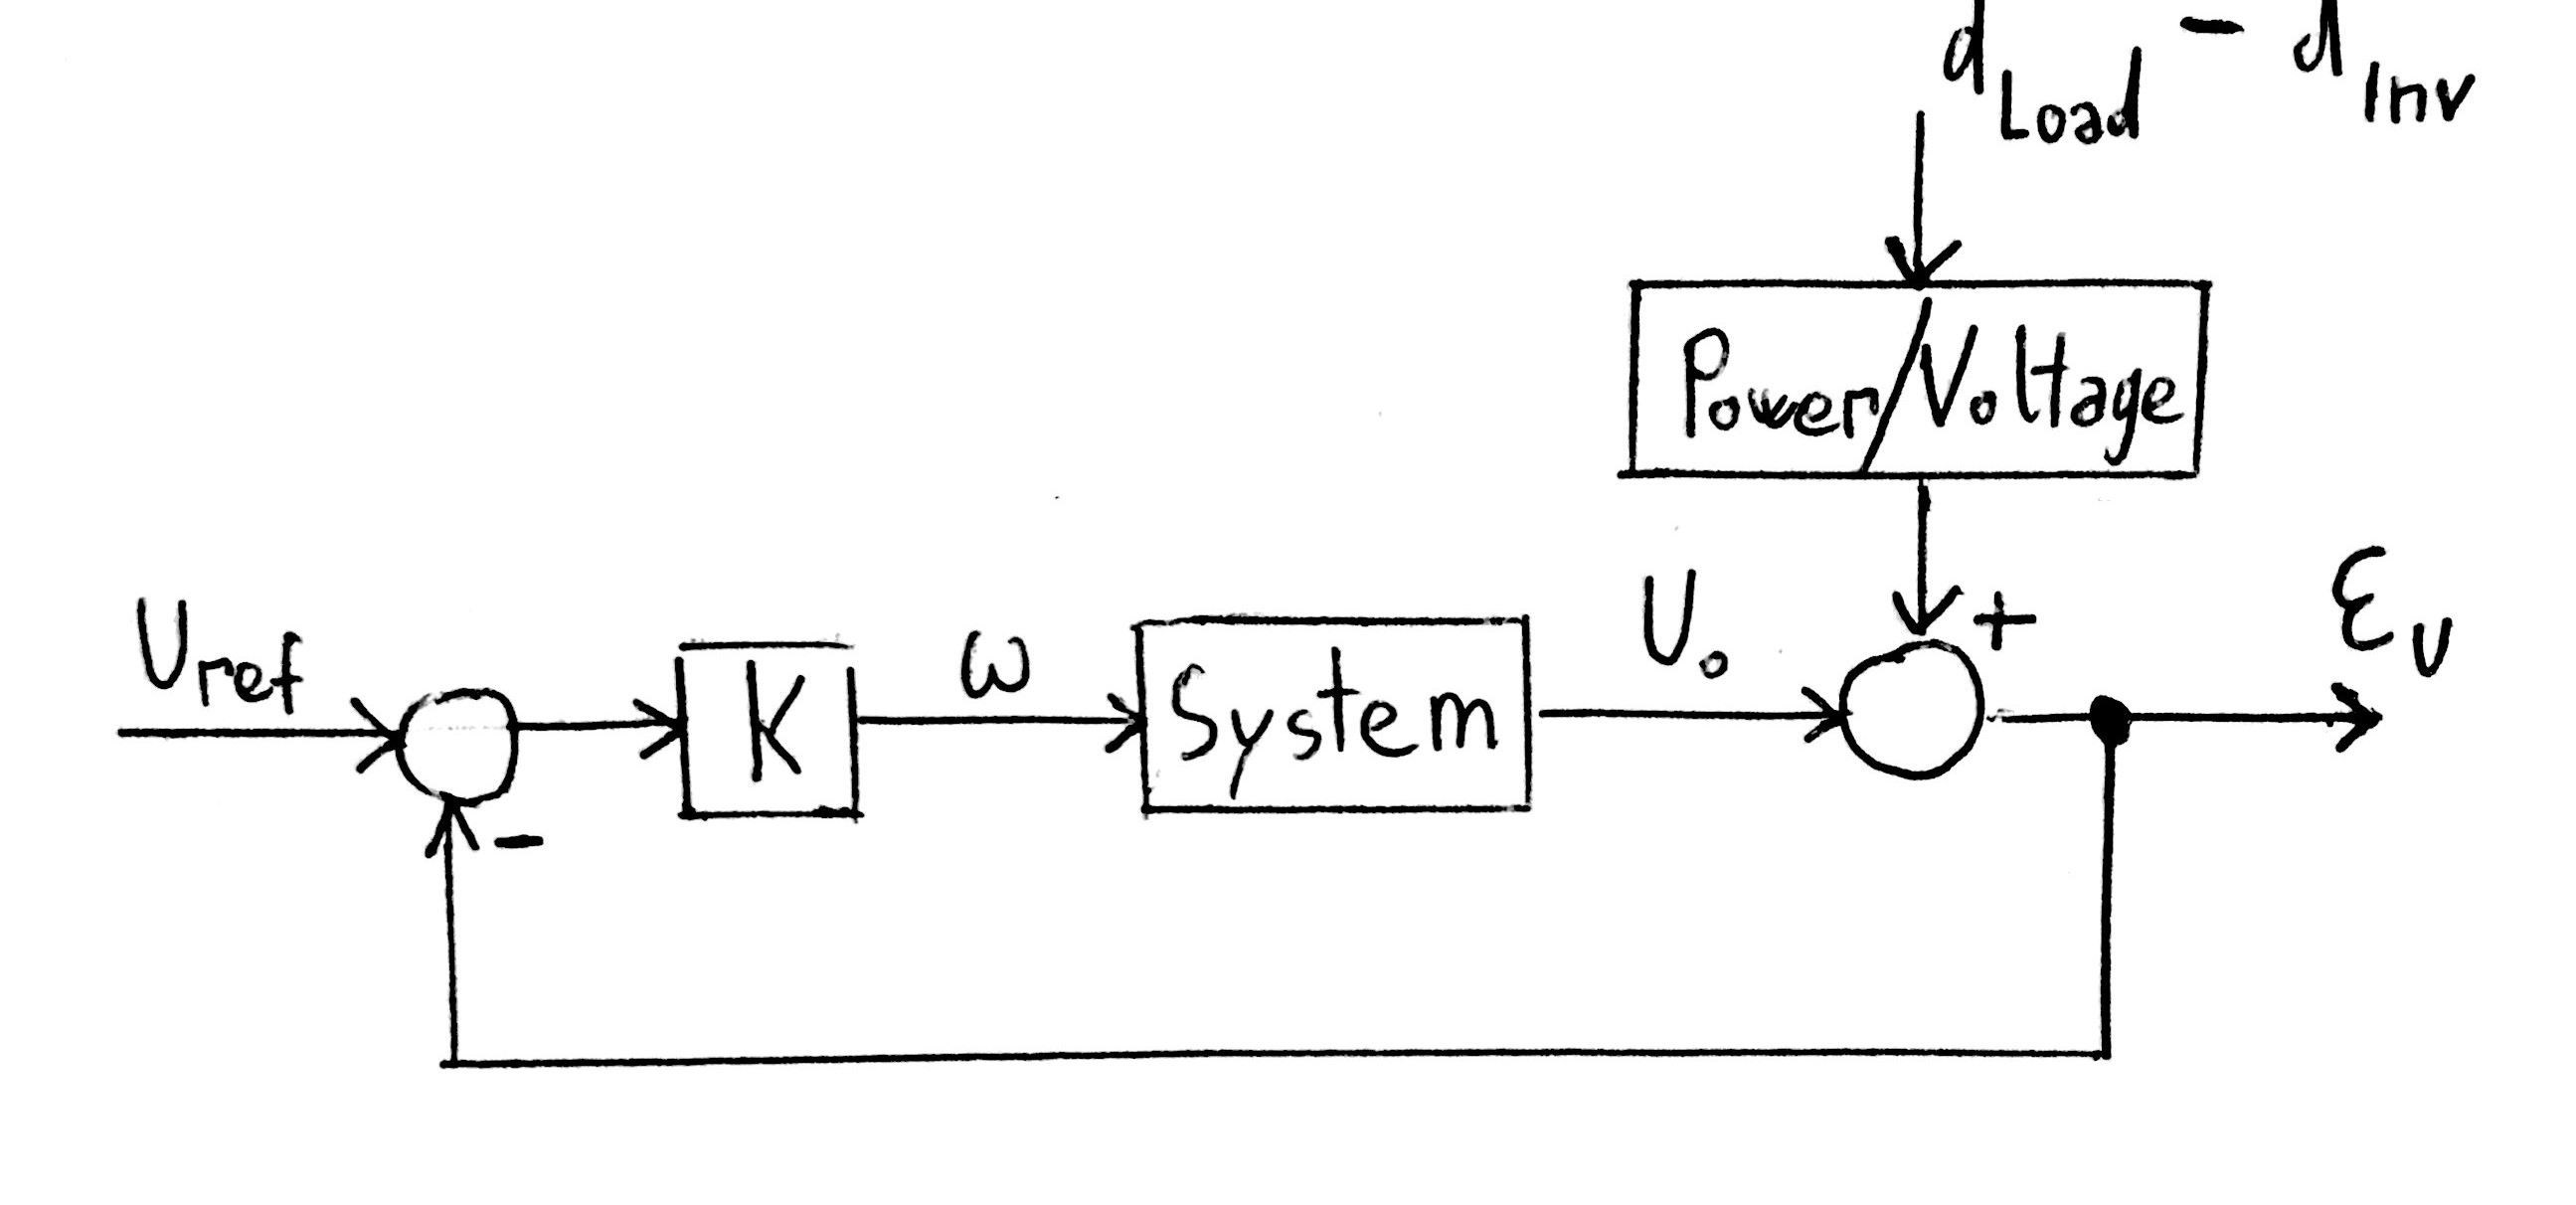
\includegraphics[width=0.65\textwidth]{rapport/billeder/blok_simplified}
%\caption{Simplified closed-loop system for the genset}
%\label{fig:blok_simplified}
%\end{figure}

\begin{figure}[H]
\centering
\begin{tikzpicture}

\draw  (-4.8,2.4) rectangle (-2.8,1.6);

\draw [-latex] (-2,4) rectangle (1.2,3.2);

\node at (-0.4,3.6) {\normalsize{Power/Voltage(s)}};
\node at (-3.8,2) {\normalsize{System(s)}};
\node at (-2,2.2) {\normalsize{$U_o$}};
\draw [-latex] (-0.4,2) ellipse (0.25 and 0.25);
\draw [-latex](-2.8,2) -- (-0.6,2);
\draw [-latex](-0.4,3.2) -- (-0.4,2.2);
\draw [-latex] (-6.8,2.4) rectangle (-6,1.6);
\node at (-6.4,2) {C(s)};
\draw [-latex](-6,2) -- (-4.8,2);
\node at (-5.6,2.2) {\large{$\omega$}};
\node at (-0.2,2.4) {$+$};
\draw [-latex] (-7.8,2) ellipse (0.25 and 0.25);
\draw [-latex](-7.54,2) -- (-6.8,2);
\draw [-latex](-0.4,4.8) -- (-0.4,4);
\node at (-0.4,5) {$d_{Load}-d_{Inv}$};
\draw [-latex](-8.8,2) -- (-8,2);
\node at (-9.2,2.2) {\normalsize{$U_{ref} = \footnotesize{0}$}};
\draw [-latex](-0.17,2) -- (1.6,2);
\node at (0.6,2.2) {\large{$\epsilon_v$}};
\draw [-latex](0.6,2) -- (0.6,0.6) -- (-7.8,0.6) -- (-7.8,1.77);
\node at (-7.6,1.6) {$-$};
\node at (-7.2,2.2) {\normalsize{$U_i$}};
\end{tikzpicture}
\caption{Simplified closed-loop system of the genset.}
\label{fig:blok_simplified}
\end{figure}

The subsystem denoted by 'System' is the plant, in other words, the transfer function derived between the mechanical angular velocity and the voltage output of the genset.


\begin{minipage}[t]{0.20\textwidth}
Where\\
\hspace*{8mm} $\omega$ \\
\hspace*{8mm} $U_o$ \\
\hspace*{8mm} $U_i$ \\
\hspace*{8mm} $U_{ref}$ \\
\hspace*{8mm} $d_{Load}-d_{Inv}$ \\
\hspace*{8mm} and $\epsilon_U$ 
\end{minipage}
\begin{minipage}[t]{0.68\textwidth}
\vspace*{2mm}
is the angular velocity output of the controller,\\
is the output voltage of the genset, \\
is the input voltage signal of the controller, \\
is the reference for the system, \\
is the disturbance affecting the system , \\
is the change(error) in the output voltage of the closed-loop controlled system. 

\end{minipage}
\begin{minipage}[t]{0.10\textwidth}
\vspace*{2mm}
\textcolor{White}{te}$\unit{\frac{rad}{s}}$\\
\textcolor{White}{te}$\unit{V}$\\
\textcolor{White}{te}$\unit{V}$\\
\textcolor{White}{te}$\unit{V}$\\
\textcolor{White}{te}$\unit{W}$\\
\textcolor{White}{te}$\unit{V}$
\end{minipage}

The block called 'Power/Voltage' serves as a conversion from power to voltage, since the disturbance applied to the system is in watts. Furthermore, it should be noted that the controller takes an input as voltage and creates a modified angular velocity input for the plant. Therefore the plant can be described as a SISO(Single Input Single Output) system according to the transfer funtion in \eqref{eq:tf_system}. 

\begin{equation}
\label{eq:tf_system}
G_{System}(s) = \frac{U_o(s)}{\omega(s)} = \frac {29.27s}{s^2 + 3.4s + 52.5} \unit{\cdot}
\end{equation}

The simplified plant will now be used to develop the controller. 
  

\subsection{Continuous state-space representation of the plant}
\label{ss_representation}

The above-mentioned transfer function can be represented as a two dimensional state-space system such as: 

\begin{equation}
  \label{eq:ss_sys1}
    \mathbf{\dot{x}(t)} = \mathbf{A} \mathbf{x}(t) + \mathbf{B} u(t)
  \end{equation}
\begin{equation}
  \label{eq:ss_sys2}
    y(t) = \mathbf{C} \mathbf{x}(t) + \mathbf{D} u(t)
  \end{equation}


\begin{minipage}[t]{0.20\textwidth}
Where\\
\hspace*{8mm} $\mathbf{A}$ \\
\hspace*{8mm} $\mathbf{B}$ \\
\hspace*{8mm} $\mathbf{C}$ \\
\hspace*{8mm} $\mathbf{D}$ \\
\hspace*{8mm} $\mathbf{x}$  \\
\hspace*{8mm} $y$  \\
\hspace*{8mm} and $u$  
\end{minipage}
\begin{minipage}[t]{0.68\textwidth}
\vspace*{2mm}
is the system matrix with a dimension: $\mathbb{R}^{(2 \times 2)}$,\\
is the input matrix with a dimension: $\mathbb{R}^{(2 \times 1)}$, \\
is the output matrix with a dimension: $\mathbb{R}^{(1 \times 2)}$, \\
is the feed-forward matrix with a dimension: $\mathbb{R}^{(1 \times 1)}$, \\
is the state vector with a dimension: $\mathbb{R}^{(2 \times 1)}$, \\
is the 1-dimensional output of the system, \\
is the 1-dimensional input of the system. 

\end{minipage}
\begin{minipage}[t]{0.10\textwidth}
\vspace*{2mm}
\textcolor{White}{te}$\unit{\cdot}$\\
\textcolor{White}{te}$\unit{\cdot}$\\
\textcolor{White}{te}$\unit{\cdot}$\\
\textcolor{White}{te}$\unit{\cdot}$\\
\textcolor{White}{te}$\unit{\cdot}$\\
\textcolor{White}{te}$\unit{V}$\\
\textcolor{White}{te}$\unit{\frac{rad}{s}}$
\end{minipage}

For the specific representation of the transfer function in \eqref{eq:tf_system}, the system consists of the following matrices: 

  \begin{equation}
  \label{eq:system_matrices_}
	\mathbf{A}
	 =   
    \begin{bmatrix}
    -3.40 & -52.05 \\
     1 & 0
\end{bmatrix}
;
\textcolor{White}{teeee}
\mathbf{B}
	 =   
    \begin{bmatrix}
    1 \\
    0
\end{bmatrix}
;
\textcolor{White}{teeee}
\mathbf{C}
	 =   
    \begin{bmatrix}
    29.27 & 0
\end{bmatrix}
;
\textcolor{White}{teeee}
\mathbf{D}
	 =   
    \begin{bmatrix}
    0
\end{bmatrix}
  \end{equation}

\subsection{State-space representation of the disturbance}
\label{statespace_disturbance}

Although there are several different ways to describe disturbances in control systems, in the presented report one approach is to assume that the power-flow of the inverter and the load can be described by differential equations. It is worth mentioning again that the behavior of the two different disturbances are significantly different. While the additional power-flow from the inverter can be approximated reasonably by a slowly-varying signal, the change in the load is much faster and in most of the cases is assumed to be completely unknown. Despite of the fact that there might be big changes in the load, in the introduction, and while introducing the principle of disturbances in state space, it is assumed to be constant. 

%\begin{figure}[H]
%\centering
%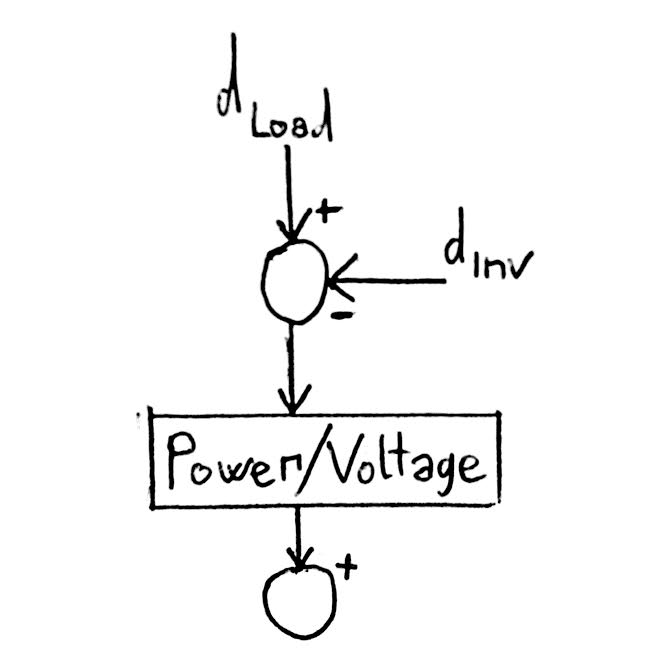
\includegraphics[width=0.3\textwidth]{rapport/billeder/disturbances}
%\caption{Disturbances acting on the plant}
%\label{fig:disturbances}
%\end{figure}

\begin{figure}[H]
\centering
\begin{tikzpicture}

 \draw [-latex] (-0.4,2) ellipse (0.25 and 0.25);
 \draw [-latex] (-2,4) rectangle (1.2,3.2);
 \node at (-0.4,3.6) {\normalsize{Power/Voltage(s)}};
\draw [-latex](-0.4,3.2) -- (-0.4,2.2);
 \node at (-0.2,2.4) {$+$};
 \draw [-latex] (-0.4,5) ellipse (0.25 and 0.25);
\draw [-latex](-0.4,4.75) -- (-0.4,4);
\draw [-latex](-0.4,6) -- (-0.4,5.22);
\node at (-0.4,6.4) {$d_{Load}$};
\draw [-latex](0.8,5) -- (-0.15,5);
\node at (1.4,5) {$d_{Inv}$};
\node at (-0.2,5.4) {$+$};
\node at (0,4.8) {$-$};
\end{tikzpicture}
\caption{Disturbances acting on the plant.}
\label{fig:disturbances}
\end{figure}

As can be seen in \figref{fig:disturbances}, a conversion is required from power to voltage with certain dynamics. However when introducing the disturbances in state space, this dynamic behaviour is neglected and is taken into consideration in the simulation instead. Furthermore, the disturbances acting on the plant will be denoted by $d$ in order to make referencing easier in the further description . 

The disturbance that enters the state-space system can be considered as: 
\begin{equation}
  \label{eq:ss_dist_intro}
    \mathbf{\dot{x}(t)} = \mathbf{A} \mathbf{x}(t) + \mathbf{B} [u(t) + d(t)]
  \end{equation}

In \eqref{eq:ss_dist_intro} $d(t)$ is the disturbance signal which can be characterized by a specific differential equation or transfer function, which can be represented as an individual state-space system. Since the disturbance does not take any inputs, it only provides input for the state-space system of the plant according to \eqref{eq:ss_dist_intro}. The system for the disturbance is called an exo-system and is therefore represented in a form as follows:
%
\begin{equation}
  \label{eq:ss_exo1}
    \mathbf{\dot{x}_d(t)} = \mathbf{A_d} \mathbf{x_d}(t)
  \end{equation}
%
\begin{equation}
  \label{eq:ss_exo2}
    d(t) = \mathbf{C}_d \mathbf{x}_d(t)
  \end{equation}
%
The relation between a state-space model and its transfer function can be described by 
%
\begin{equation}
  \label{eq:ss_tf}
    D(s) = \mathbf{C}_d(s\mathbf{I}-\mathbf{A_d})^{-1} \mathbf{x_d}(0) = \mathbf{C}_d \frac{Adj(s\mathbf{I}-\mathbf{A_d})}{det(s\mathbf{I}-\mathbf{A_d})} \mathbf{x_d}(0) = \frac{f(0,s)}{\Gamma_d(s)}
  \end{equation}
  % 
\begin{minipage}[t]{0.20\textwidth}
Where\\
\hspace*{8mm} $f(0,s)$ \\
\hspace*{8mm} $\Gamma_d(s)$ \\
\hspace*{8mm} and $\mathbf{x_d}(0)$  
\end{minipage}
\begin{minipage}[t]{0.68\textwidth}
\vspace*{2mm}
is the polynomial in s arises because of initial conditions,\\
is called the disturbance generating polynomial, \\
is the vector of initial conditions. 

\end{minipage}

As can be seen, the disturbance generator is the characteristic polynomial of $A_d$. In order to build up the state-space matrices, \eqref{eq:ss_tf} can be split into two equations:
%
\begin{equation}
  \label{eq:ss_tf1}
    \Gamma_d(s) = det(s\mathbf{I}-\mathbf{A_d}) 
  \end{equation}
%
Where $\Gamma_d(s)$ can be considered as the denominator of the transfer function of the disturbance. Therefore $A_d$ can be found easily by solving a simple eigenvalue problem. The equation for the numerator can be written as: 
%
\begin{equation}
  \label{eq:ss_tf2}
    f(0,s) = \mathbf{C}_d Adj(s\mathbf{I}-\mathbf{A_d}) \mathbf{x_d}(0)
  \end{equation}
%
Where $f(0,s)$ represents the numerator of the transfer function of disturbance. $\mathbf{A_d}$ is known from \eqref{eq:ss_tf1} and $\mathbf{x_d}(0)$ consists of the priorly defined initial conditions. Therefore $\mathbf{C}_d$ can be calculated which means that the state representation of the disturbance becomes fully defined. It should be noted however, that even from \eqref{eq:ss_tf} or \eqref{eq:ss_tf2} it can be clearly seen, that if there is not any initial conditions defined for the disturbance, the elements of $\mathbf{C}_d$ are going to be zero. This directly means that there will not be any output of the exo-system, therefore there will not be any disturbance appearing on the output signal. 

According to \eqref{eq:ss_dist_intro}, \eqref{eq:ss_exo1} and \eqref{eq:ss_exo2}, the system can be rewritten in matrix form with the modified matrices including the exo-system: 
%
\begin{equation}
\label{eq:ss_dist1}
\begin{bmatrix}
    \mathbf{\dot{x}} \\
    \mathbf{\dot{x_d}} 
\end{bmatrix}
=
\underbrace{
 \begin{bmatrix}
    \mathbf{A} & \mathbf{B}\mathbf{C_d} \\
    0 & \mathbf{A_d}
\end{bmatrix}
}_\text{\normalsize{$\tilde{\mathbf{A}}$}}
\underbrace{
 \begin{bmatrix}
    \mathbf{x} \\
    \mathbf{x_d}
\end{bmatrix}
}_\text{\normalsize{$\tilde{x}$}}
+
\underbrace{
 \begin{bmatrix}
    \mathbf{B}  \\
    0 &  
\end{bmatrix}
}_\text{\normalsize{$\tilde{\mathbf{B}}$}}
    u
\end{equation}

\begin{equation}
\label{eq:ss_dist2}
    d
=
\underbrace{
 \begin{bmatrix}
    \mathbf{C} & 0 
\end{bmatrix}
}_\text{\normalsize{$\tilde{\mathbf{C}}$}}
 \begin{bmatrix}
    \mathbf{x} \\
    \mathbf{x_d}
\end{bmatrix}
\end{equation}

Therefore an extended state-space model is given where both the states of the plant and the disturbance are taken into account. It should be noted however, that the augmented system is not controllable from the input $d$ because the disturbance by the exo-system is an exogenous, autonomous input. The modified system can be illustrated such as in \figref{fig:exosystem}: 

%\begin{figure}[H]
%\centering
%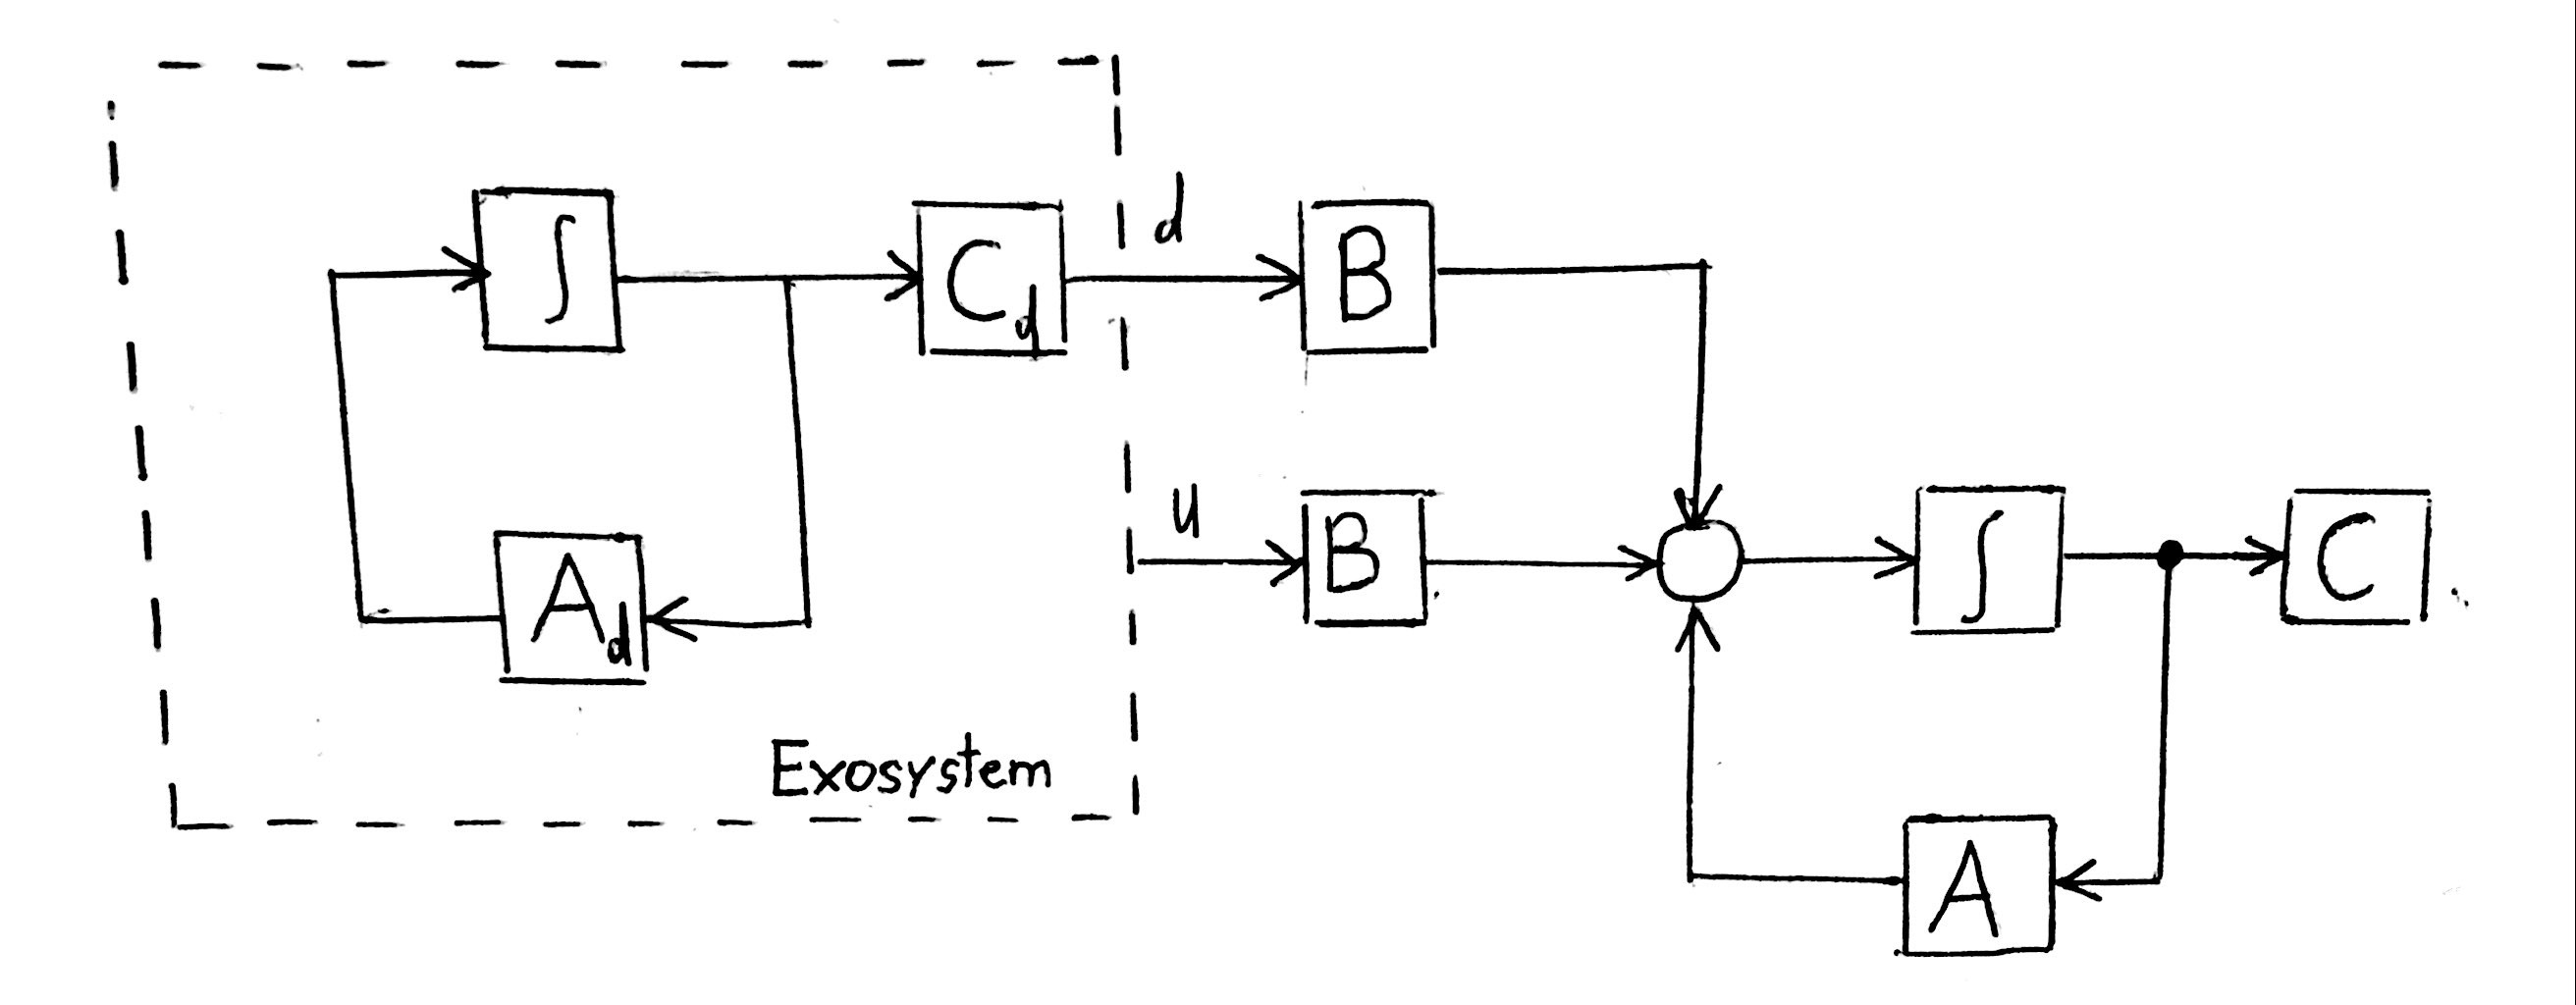
\includegraphics[width=0.7\textwidth]{rapport/billeder/exosystem}
%\caption{Exo-system as the input of the system}
%\label{fig:exosystem}
%\end{figure}


\begin{figure}[H]
\centering
\begin{tikzpicture}


 \draw [-latex] (-0.4,2) ellipse (0.25 and 0.25);
\node at (1.2,0.2) {\normalsize{$A$}};
\node at (-1.8,2) {\normalsize{$B$}};
\node at (3.2,2) {\normalsize{$C$}};
\node at (-1.8,3.4) {\normalsize{$B$}};
\node at (-5.4,2) {\normalsize{$A_d$}};
\node at (-3.6,3.4) {\normalsize{$C_d$}};
\node at (1.2,2) {\normalsize{$\int$}};

\draw [-latex] (0.8,2.4) rectangle (1.6,1.6);
\draw [-latex] (0.8,0.6) rectangle (1.6,-0.2);
\draw [-latex] (2.8,2.4) rectangle (3.6,1.6);
\draw [-latex] (-2.2,2.4) rectangle (-1.4,1.6);
\draw [-latex] (-2.2,3.8) rectangle (-1.4,3);
\draw [-latex](-1.4,2) -- (-0.6,2);
\draw [-latex](-0.15,2) -- (0.8,2);


\draw [-latex](1.6,2) -- (2.8,2);
\draw [-latex](3.6,2) -- (4.6,2);
\draw [-latex](2.2,2) -- (2.2,0.2) -- (1.6,0.2);
\draw [-latex](0.8,0.2) -- (-0.4,0.2) -- (-0.4,1.8);
\draw [-latex](-1.4,3.4) -- (-0.4,3.4) -- (-0.4,2.2);

\node at (-5.4,3.4) {\normalsize{$\int$}};

\draw [-latex] (-4,3.8) rectangle (-3.2,3);
\draw [-latex] (-5.8,3.8) rectangle (-5,3);
\draw [-latex] (-5.8,2.4) rectangle (-5,1.6);
\draw [-latex](-3.2,3.4) -- (-2.2,3.4);
\draw [-latex](-3.2,2) -- (-2.2,2);
\draw [-latex](-5,3.4) -- (-4,3.4);
\draw [-latex](-4.4,3.4) -- (-4.4,2) -- (-5,2);
\draw [-latex](-5.8,2) -- (-6.4,2) -- (-6.4,3.4) -- (-5.8,3.4);
\node at (-2.8,3.6) {\normalsize{$d$}};
\node at (-2.8,2.2) {\normalsize{$u$}};
\node at (4,2.2) {\normalsize{$y$}};
\draw [dash pattern=on 2pt off 3pt on 4pt off 4pt] (-7.6,4.4) rectangle (-3.2,1);
\node at (-4.2,1.2) {\normalsize{$Exosystem$}};
\end{tikzpicture}

\caption{Exo-system as the input of the system.}
\label{fig:exosystem}
\end{figure}





\subsection{Disturbances affecting the system}
\label{disturbances}

In \secref{statespace_disturbance}, the two kinds of disturbances were introduced, namely the load and the inverter. The inverter, as it was mentioned, provides a slowly changing power flow that can be approximated as a sinusoidal shown in \eqref{eq:dist1} : 

\begin{equation}
  \label{eq:dist1}
    d_{inv}(t) = \alpha sin(\omega t)
  \end{equation}

By solving \eqref{eq:ss_tf1} and \eqref{eq:ss_tf2} the state space system can be constructed: 


\begin{equation}
\label{eq:exo_statespace}
 \begin{bmatrix}
    \dot{x}_{d1} \\
    \dot{x}_{d2}
\end{bmatrix}
=
 \begin{bmatrix}
    0 & \omega^2 \\
    -\omega^2 & 0
\end{bmatrix}
 \begin{bmatrix}
    x_{d1} \\
    x_{d2}
\end{bmatrix}
\end{equation}

\begin{equation}
\label{eq:ss_dist2}
    d
=
 \begin{bmatrix}
    1 & 0 
\end{bmatrix}
 \begin{bmatrix}
    x_{d1} \\
    x_{d2}
\end{bmatrix}
\end{equation}

The characteristic polynomial of the sinusoidal disturbance system, as expected is: 

\begin{equation}
  \label{eq:distpoly}
    \Gamma_{inverter}(s) = det(s\mathbf{I}-\mathbf{A_d}) = s^2 + \omega^2 
  \end{equation}
  
%The case of the load however is significantly different from the case of the inverter. The load is, as mentioned, usually unknown and can produce big changes. The fact that the behaviour of the load is completely unknown in reality cannot be neglected, however in the simulation a constant load is described to show how the system can reject it. The reason behind making a disturbance that dramatically affects the voltage output of the system is that if the load was constant, a slowly varying inverter power flow would never cause changes on the output. That is because the AVR and the other inner controllers can easily handle slow disturbances such as the inverter power flow. 


In order to construct the combination of the two disturbances, the following rule applies: 

\begin{equation}
  \label{eq:combined_dist}
  d(t) = d_{inv}(t) + d_{load}(t) = \Gamma_{inv}(s)\Gamma_{load}(s)
  \end{equation}
  
As can be seen in \eqref{eq:combined_dist}, the combined disturbance system can be calculated by multiplying the disturbance generating polynomials for $d_{inv}(t)$ and $d_{load}(t)$. Thus, the final form of the disturbance becomes: 

\begin{equation}
  \label{eq:dist_final}
  d(t) = d_{inv}(t) + d_{load}(t) = c + \alpha sin(\omega t)
  \end{equation}

that is a slowly-varying sinusoidal disturbance with an offset. 
\section{Controller design with exosystem in continuous time}
\label{system_design}

The main goal of the control is to make the system react faster to changes in the load. Along with the the inverter power, load changes affect the system as disturbances. The main task is then to reject these disturbances and make the closed-loop dynamics react faster to sudden changes coming from the load. This directly means that by applying a controller to the system, the error in voltage will be reduced on the output, and will go to zero as fast as it is possible. 
The dynamics of the system are changed through feeding back the states, thus the feedback law for the overall closed loop system becomes: 

\begin{equation}
  \label{eq:feedbacklaw}
  u = r + \mathbf{Fx}
  \end{equation}

It should be noted however, that due to the separation principle the state feedback and the observer problem can be handled independently and furthermore, while designing the state feedback for the system, disturbances can be neglected on the system. The block diagram of the system then simplifies to: 

%\begin{figure}[H]
%\centering
%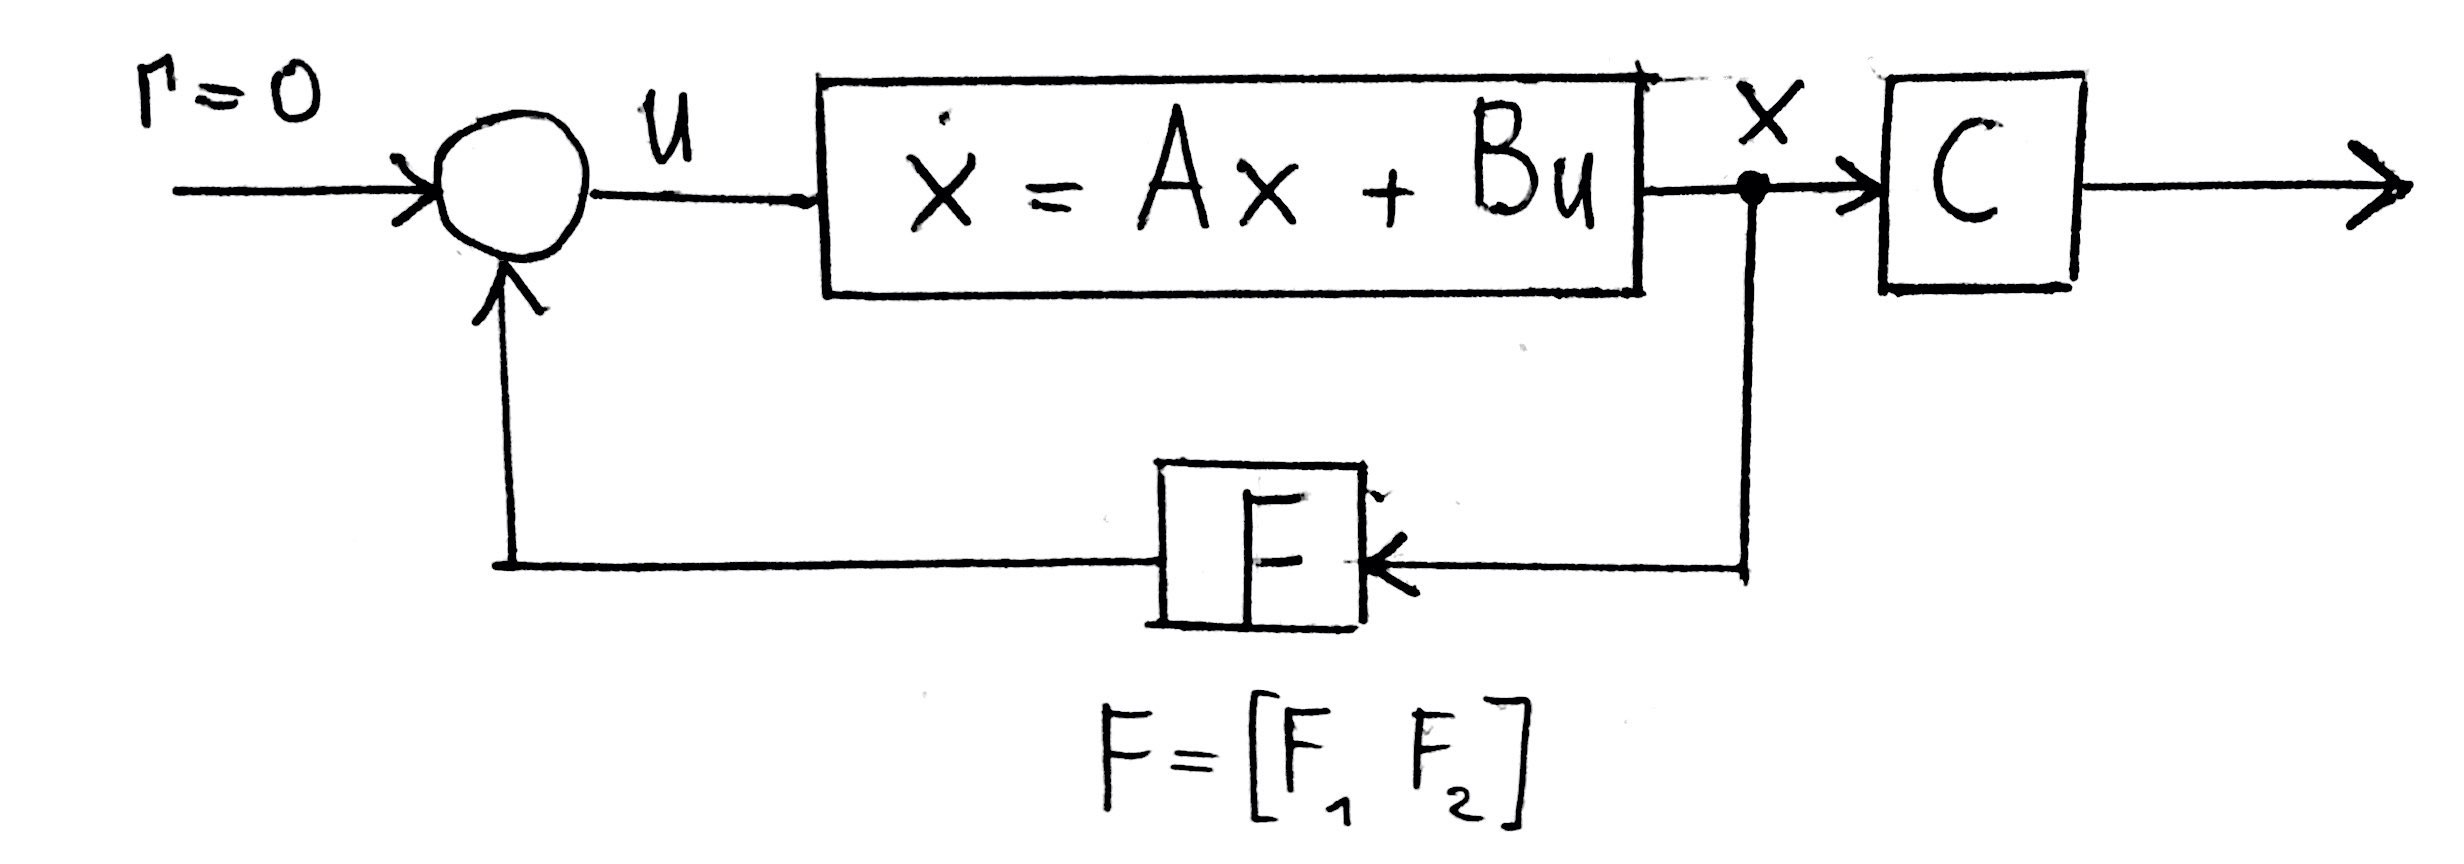
\includegraphics[width=0.55\textwidth]{rapport/billeder/stateblock}
%\caption{State feedback}
%\label{fig:stateblock}
%\end{figure}

\begin{figure}[H]
\centering
\begin{tikzpicture}

 \draw [-latex] (-0.4,2) ellipse (0.25 and 0.25);
\node at (2.8,2) {\normalsize{$\mathbf{\dot{x}(t)} = \mathbf{A} \mathbf{x}(t) + \mathbf{B} u(t) $}};

\draw [thin] (0.8,2.4) rectangle (4.8,1.6);
 \node at (6.2,2) {\normalsize{$\mathbf{C}$}};
\draw [thin] (5.8,2.4) rectangle (6.6,1.6);
 \node at (2.4,0.4) {\normalsize{$\mathbf{F}$}};


\draw [thin] (2,0.8) rectangle (2.8,0);
\draw [thin](4.67,2) node (v1) {};

\draw [-latex](v1) -- (5.82,2);
\draw [-latex](6.6,2) -- (7.6,2);
\draw [-latex](5.4,2) -- (5.4,0.4) -- (2.8,0.4);
\draw [-latex](-0.15,2) -- (0.8,2);
\draw [-latex](2,0.4) -- (-0.4,0.4) -- (-0.4,1.8);
\draw [-latex](-1.4,2) -- (-0.6,2);
\node at (0.2,2.2) {\normalsize{$u$}};
\node at (5.4,2.2) {\normalsize{$\mathbf{x}$}};
\node at (7.2,2.2) {\normalsize{$y$}};
\node at (-1.6,2.2) {\normalsize{$r = 0$}};
\end{tikzpicture}
\caption{State feedback}
\label{fig:statefeedback}
\end{figure}


Therefore the control problem simplifies to the problem of finding new locations of the eigenvalues such as:

\begin{equation}
  \label{eq:distpoly}
    det(s\mathbf{I}-(\mathbf{A} + \mathbf{B} \mathbf{F}))
  \end{equation}

Since these eigenvalues define the closed-loop dynamics, the main design decision is to find where to place them. The original poles of the system are: 
\begin{equation}
  \label{eq:original poles}
  p_{1;2} = -1.7 \pm j7
  \end{equation}

It can be clearly seen from \eqref{eq:original poles} that the system has a complex conjugate pole pair on the left-hand side of the real axis, therefore the system is stable, as it was expected. By placing the poles more than four times further, the following pole configuration can be achieved: 

\begin{equation}
  \label{eq:desired_poles}
  p_{F_{1;2}} = -8 \pm j7
  \end{equation}
  
The step response with state feedback yields: 
\begin{figure}[H]
\centering
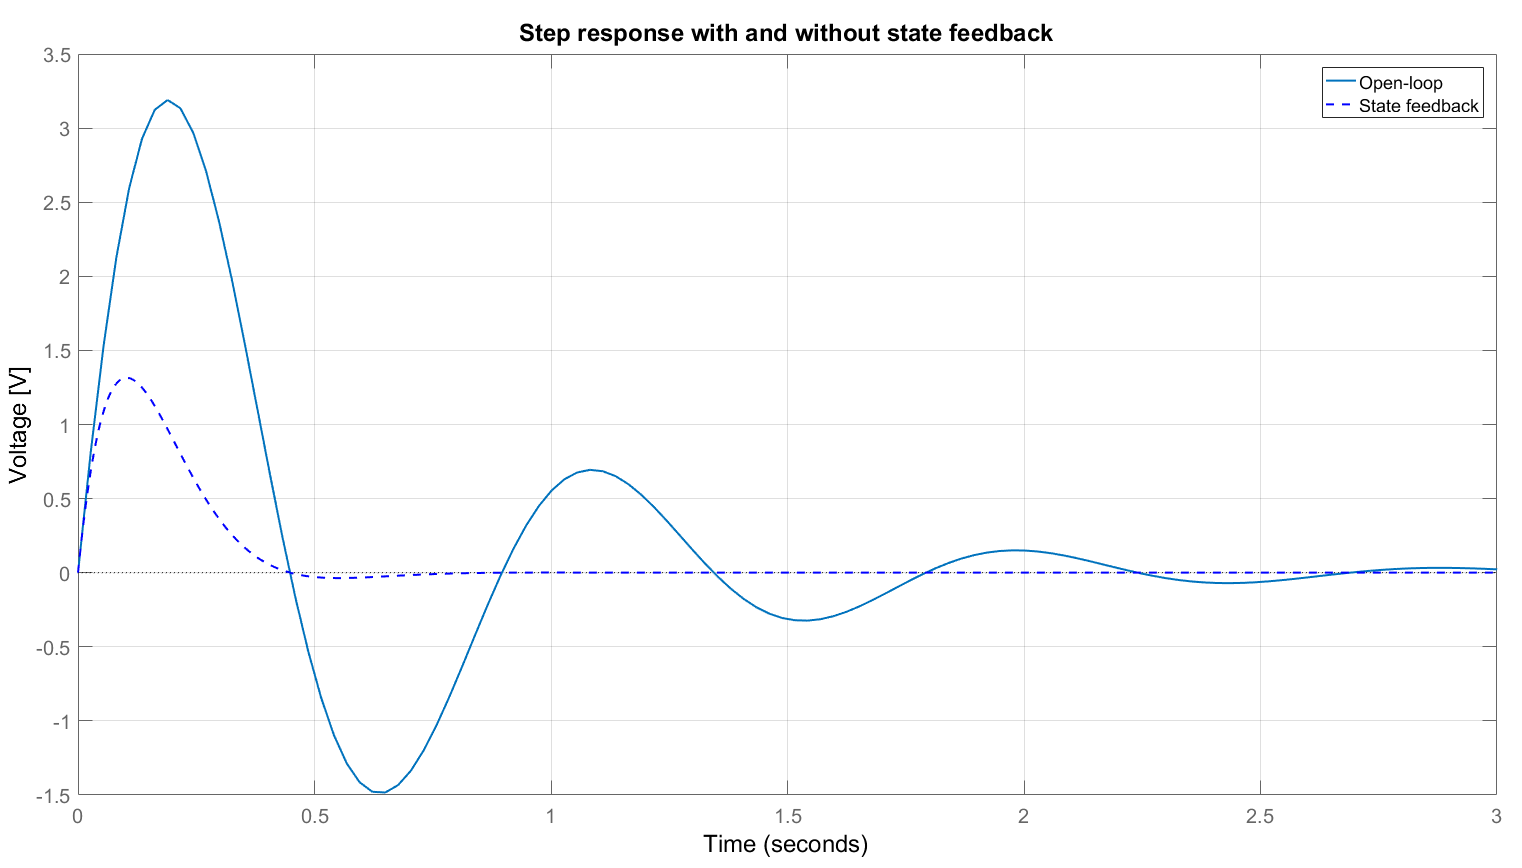
\includegraphics[width=0.85\textwidth]{rapport/billeder/statefeedback}
\caption{State feedback.}
\label{fig:statefeedback}
\end{figure}


And the state feedback gain is the following:

\begin{equation}
\label{eq:ss_dist2}
    F
=
 \begin{bmatrix}
    -12.6 & -60.95
\end{bmatrix}
\end{equation}
\subsection{Observer design}
\label{observer}

As it is shown in \figref{fig:statefeedback}, it is possible to find a state feedback law that gives closed-loop eigenvalues with desired dynamics and a condition that all states are measured. Even if all states are measured or measurable, the disturbances has to be taken into consideration while designing the observer. 

If a system is observable, it is possible to recover the states from measurements of the input and output of the system. The feedback law is exactly the same as in \eqref{eq:feedbacklaw} with the exception that now the disturbance is also considered and due to the separation principle it is sufficient to design the observer without the state feedback. The purpose of the observer is now to reconstruct both the system states $\mathbf{x}$ and the disturbance $d$ from the input and the output. Since the disturbance has an effect on the output, it is observable from y. Furthermore, $d$ is generally unknown, thus it is reasonable to estimate it with a help of an observer. It is important to mention that although the disturbance cannot be measured, information about its structure and periodicity are assumed to be available in this simulation. 

The system with the observer and state feedback can be represented as follows: 

%\begin{figure}[H]
%\centering
%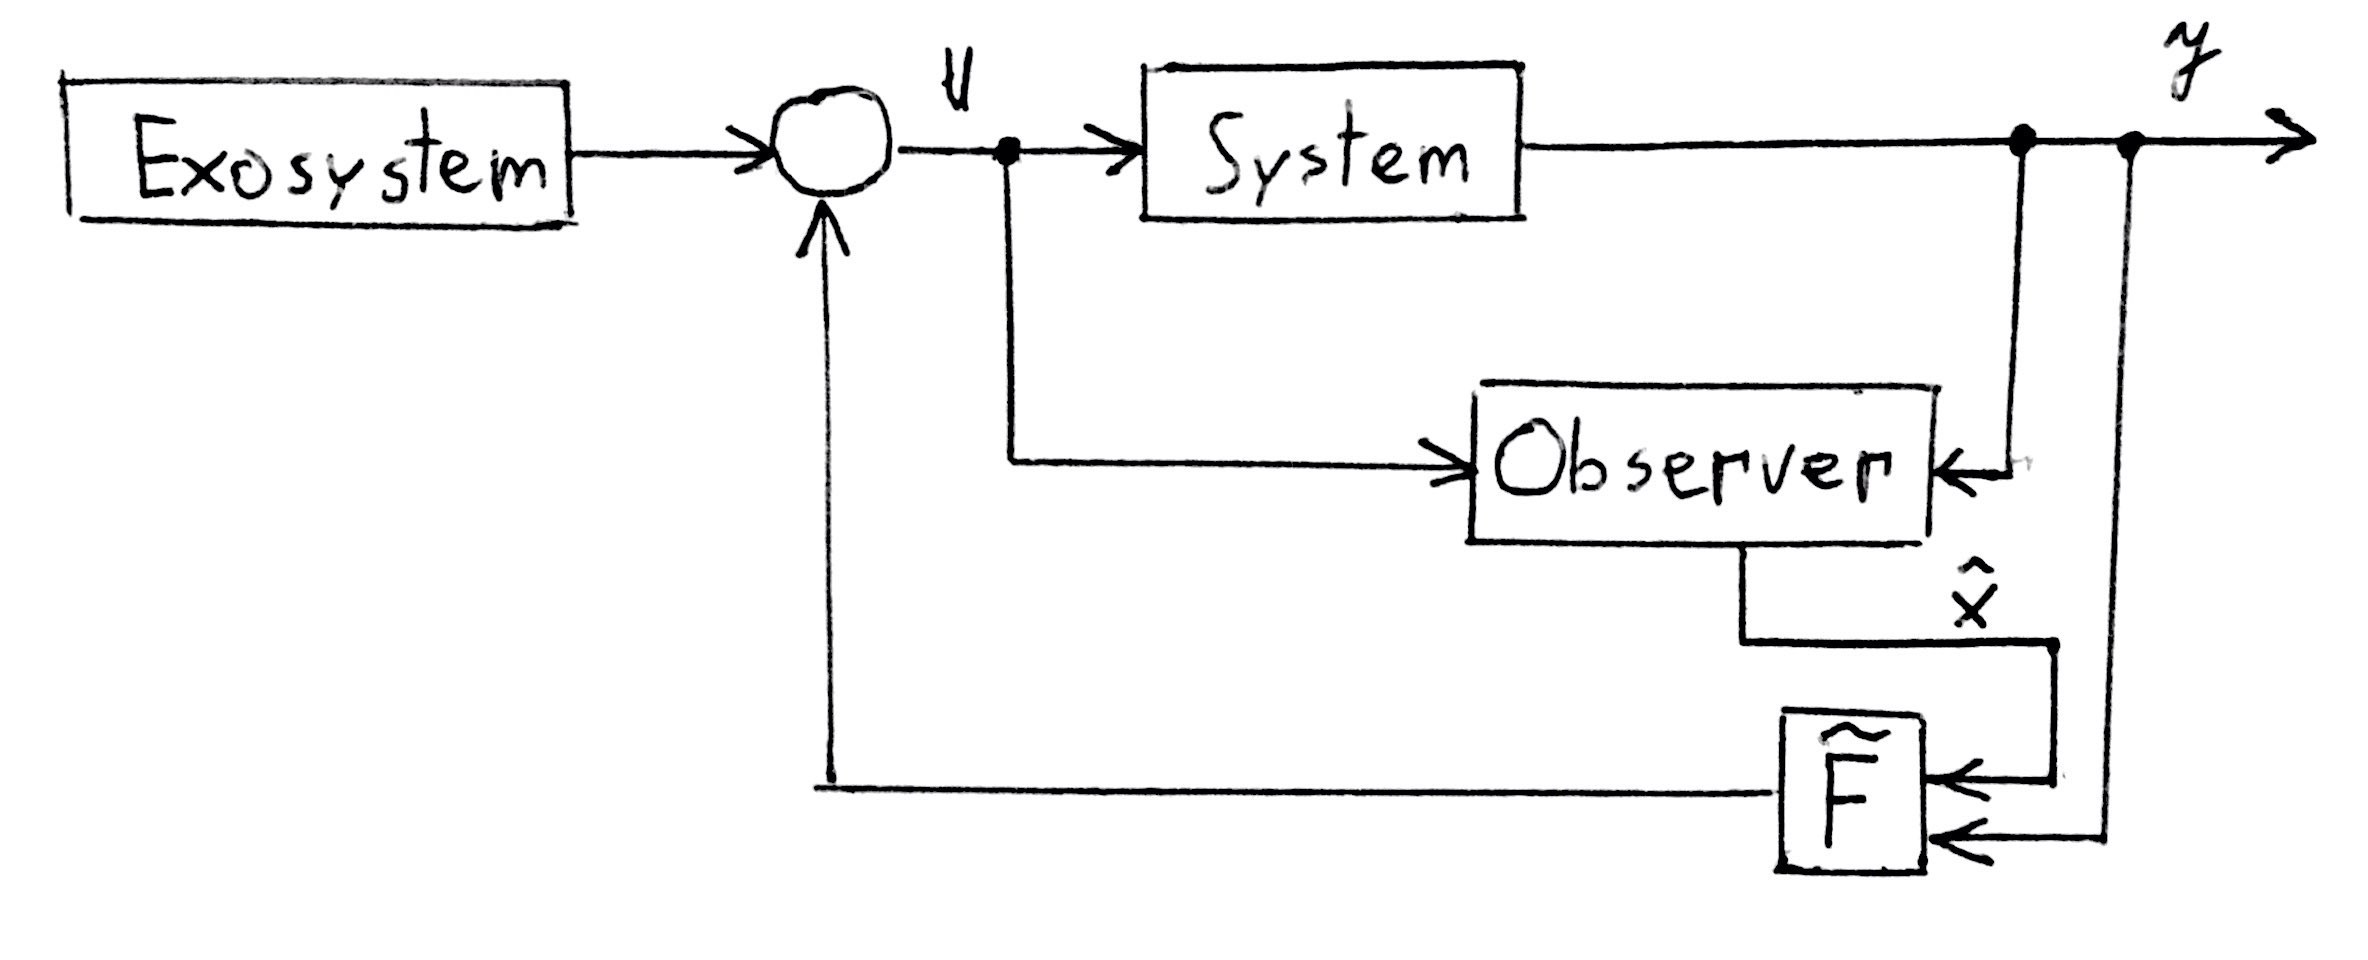
\includegraphics[width=0.65\textwidth]{rapport/billeder/observerblock}
%\caption{State feedback}
%\label{fig:observerblock}
%\end{figure}


\begin{figure}[H]
\centering
\begin{tikzpicture}


 \draw [-latex] (-1.2,2) ellipse (0.25 and 0.25);
 \node at (2,2) {\normalsize{System}};
\draw [-latex] (1,2.4) rectangle (3,1.6);
 \node at (2,0.4) {\normalsize{Observer}};


\draw [-latex] (1,0.8) rectangle (3,0);
\draw [-latex](-0.95,2) -- (1,2);
\draw [-latex](0.4,2) -- (0.4,0.4) -- (1,0.4);
\draw [-latex](3,2) -- (5.2,2);
\draw [-latex](3.6,2) -- (3.6,0.4) -- (3,0.4);

 \node at (0.8,-1) {\normalsize{State Feedback}};
 
 
\draw [-latex] (-0.6,-0.6) rectangle (2.2,-1.4);
\draw [-latex](2.6,0) -- (2.6,-0.8) -- (2.2,-0.8);
\draw [-latex](4.2,2) -- (4.2,-1.2) -- (2.2,-1.2);
\draw [-latex](-0.6,-1) -- (-1.2,-1) -- (-1.2,1.8);

\node at (-3,2) {\normalsize{Exosystem}};

\draw [-latex] (-4.2,2.4) rectangle (-2,1.6);
\draw [-latex](-2,2) -- (-1.4,2);
\node at (4.8,2.2) {\normalsize{$y$}};
\node at (0,2.2) {\normalsize{$u$}};

\node at (2.8,-0.4) {\normalsize{$\mathbf{\tilde{x}}$}};

\end{tikzpicture}
\caption{State feedback}
\label{fig:observerblock}
\end{figure}

Therefore the state-space system description becomes: 

\begin{equation}
\label{eq:ss_obs1}
\frac{d}{dt}
\begin{bmatrix}
    \mathbf{\tilde{x}} \\
    \mathbf{\tilde{x_d}} 
\end{bmatrix}
=
 \begin{bmatrix}
    \mathbf{A} & \mathbf{B}\mathbf{C_d} \\
    0 & \mathbf{A_d}
\end{bmatrix}
 \begin{bmatrix}
    \mathbf{\tilde{x}} \\
    \mathbf{\tilde{x_d}}
\end{bmatrix}
+
 \begin{bmatrix}
    \mathbf{B}  \\
    0 &  
\end{bmatrix}
    u
    +
 \begin{bmatrix}
    \mathbf{L_1}  \\
    \mathbf{L_2}  
\end{bmatrix}
 \begin{bmatrix}
    y - \mathbf{C}\mathbf{\tilde{x}}
\end{bmatrix}
\end{equation}

The modified control law:

\begin{equation}
  \label{eq:ss_obs2}
  u =  \mathbf{F} \mathbf{\tilde{x}_{combined}} 
  =
 \begin{bmatrix}
    \mathbf{F} & \mathbf{-C_d}  
\end{bmatrix}
 \begin{bmatrix}
\mathbf{\tilde{x}}  \\
\mathbf{\tilde{x_d}}
\end{bmatrix}
  \end{equation}
  
As can be seen in \eqref{eq:ss_obs2}, the feedback gain is extended in order to reproduce the disturbance and subtract it from the output. 
  
The control problem of finding the appropriate observer feedback gains simplifies to the problem of finding new locations of the closed-loop eigenvalues of the observer such as:

\begin{equation}
  \label{eq:distpoly}
    det(s\mathbf{I}-(\mathbf{\tilde{A}} + \mathbf{\tilde{L}} \mathbf{\tilde{C}}))
  \end{equation}

Since the poles of the observer should not have any effect on the system, in other words, it is undesirable to introduce new dominant poles in the system, as a rule of thumb the poles should be placed 2 to 6 times further to the left-hand side along the real axis from the poles of the state feedback. By making the observer dynamics react fast, the difference between the estimated and the real output will converge faster to zero. According to \eqref{eq:desired_poles}, the poles should be placed at: 

\begin{equation}
  \label{eq:desired_poles_observer1}
  p_{L_{3;4}} = -16 \pm j7
  \end{equation}
  
and
  
\begin{equation}
  \label{eq:desired_poles_observer2}
  p_{L_{5}} = -2 +j0
  \end{equation}
  
  \begin{equation}
  \label{eq:desired_poles_observer3}
  p_{L_{6}} = -4 +j0
  \end{equation}
  

  
  
  
\subsection{Results and conclusions of the exosystem control design}
\label{Exo_result}

As can be seen in \figref{fig:sin_disturbance}, by applying the disturbance through an exosystem as an input to the original system, the slowly-varying sinusoidal appears on the output.

\begin{figure}[H]
\centering
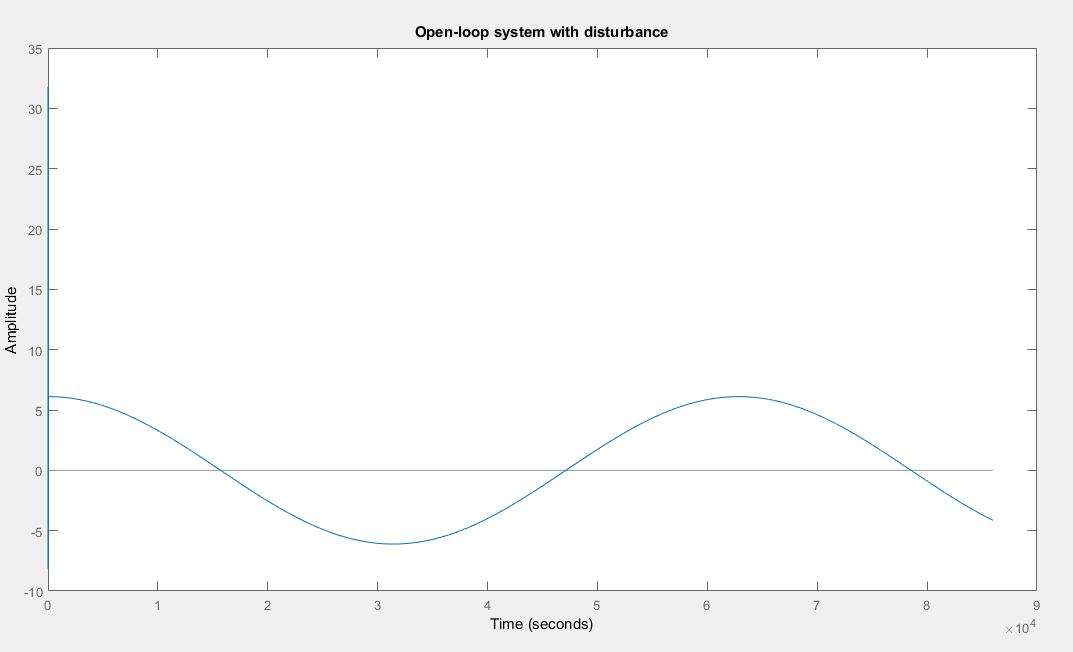
\includegraphics[width=1.1\textwidth]{rapport/billeder/temporary/sinusdist}
\caption{Slowly varying sinusoidal disturbance on the output.}
\label{fig:sin_disturbance}
\end{figure}

However, during the real-life measurements and according to the simulation of the genset, this result could never be obtained. The main reason why this result could not be achieved is that the genset with its inner AVR control can easily react to small and slow changes on the voltage, therefore would the disturbance all ready be handled by the genset and not be present on the output. 

In simulation where the genset is unable to handle the disturbance, applying the designed controller, results in the following dynamics for disturbance rejection, that are shown in \figref{fig:sin_disturbance_reject} where it is seen that the disturbance is effectively rejected. 

\begin{figure}[H]
\centering
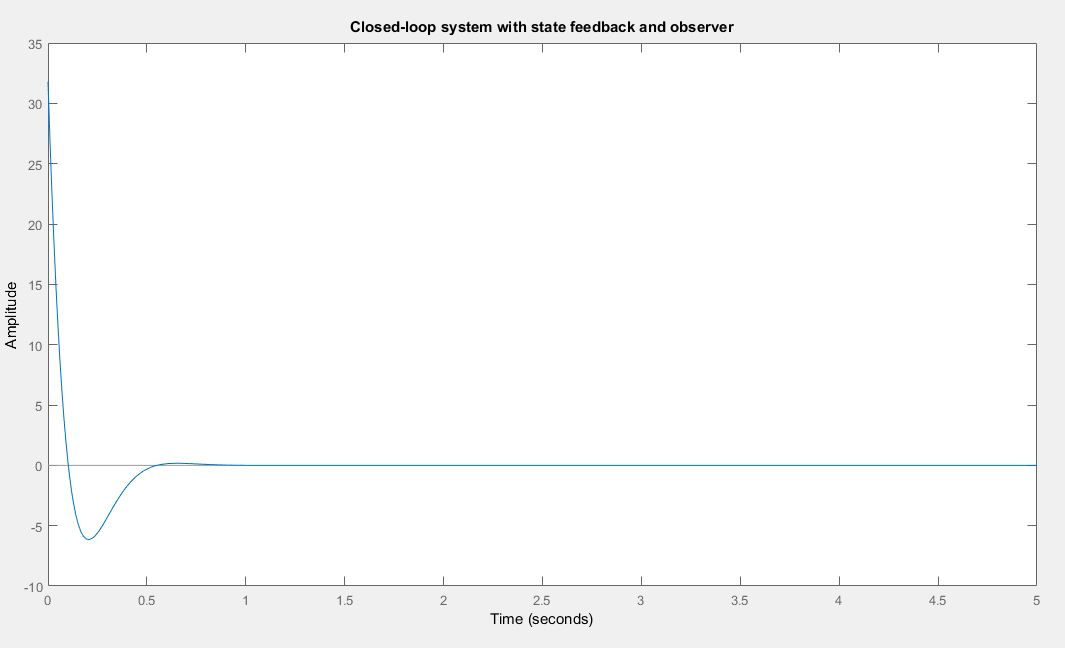
\includegraphics[width=1.1\textwidth]{rapport/billeder/temporary/eliminated_disturbance}
\caption{Sinusoidal disturbance rejected due to observer, feedback and state space control.}
\label{fig:sin_disturbance_reject}
\end{figure}

After coming to the realization that this approach does not fit reality, it was decided to put more focus on the fast varying load and make a design that can handle it in simulation and in reality. Therefore the following sections deals with a more suitable controller design. 
\section{Controller design with disturbance on the output}
\label{system_design_implementation}


As mentioned in \secref{control_intro}, a better control approach is to represent the state space model in discrete time in order to make it possible to implement on the system. In \figref{fig:block_dist}, an overview of the control design can be seen where the disturbance is on the output of the system and therefore not included in the state-space design.

\begin{figure}[H]
\centering
\begin{tikzpicture}
 \draw [-latex] (-1.4,2) ellipse (0.25 and 0.25);
 \node at (2,2) {\normalsize{System}};
\draw [-latex] (1,2.4) rectangle (3,1.6);
 \node at (2,0.2) {\normalsize{Observer}};
  \node at (2,0.6) {\normalsize{Full Order}};


\draw [-latex] (1,1) rectangle (3,-0.2);
\draw [-latex](-1.2,2) -- (1,2);
\draw [-latex](0.4,2) -- (0.4,0.4) -- (1,0.4);

\draw [-latex](4.8,2) -- (4.8,0.4) -- (3,0.4);

 \node at (0.4,-1) {\normalsize{State Feedback}};
 
 
\draw [-latex] (-1,-0.6) rectangle (1.8,-1.4);
\draw [-latex](2.6,-0.2) -- (2.6,-0.8) -- (1.8,-0.8);

\draw [-latex](-1,-1) -- (-1.4,-1) -- (-1.4,1.8);

  \node at (-3.2,2) {\normalsize{Gain}};


\draw [-latex](-2.6,2) -- (-1.6,2);
\node at (5.8,2.2) {\normalsize{$y+d$}};
\node at (0,2.2) {\normalsize{$u$}};

\node at (2.8,-0.6) {\normalsize{$\mathbf{\tilde{x}}$}};

\draw [-latex] (-3.8,2.4) rectangle (-2.6,1.6);

\draw [-latex] (-4.6,2) ellipse (0.25 and 0.25);

 \draw [-latex] (3.8,2) ellipse (0.25 and 0.25);

\draw [-latex](3,2) -- (3.6,2);
\draw [-latex](4.05,2) -- (6.2,2);
\draw [-latex](3.8,3.4) -- (3.8,2.2);



\draw [-latex](-4.35,2) -- (-3.8,2);
\draw [-latex](-5.6,2) -- (-4.8,2);
\draw [-latex](5.4,2) -- (5.4,-2.6) -- (-4.6,-2.6) -- (-4.6,1.8);

 \node at (3.8,5.4) {\normalsize{$d =d_{load}-d_{inverter}$}};
 
 \node at (4,2.4) {$+$};
\node at (-4.4,1.6) {$-$};
\node at (-5.8,2.2) {r = 0};

\draw [dash pattern=on 2pt off 3pt on 4pt off 4pt] (-2.2,3) rectangle (5.2,-1.6);
\node at (3.6,-1.4) {\normalsize{Inner control}};
\node at (3.6,-2.4) {\normalsize{Outer control}};

\draw [-latex] (2.2,4.2) rectangle (5.2,3.4);
\node at (3.8,3.8) {\normalsize{Power/Voltage}};
\draw [-latex](3.8,5) -- (3.8,4.2);
\node at (-1.2,1.6) {$+$};
\end{tikzpicture}


\caption{Block diagram of the system with disturbance.}
\label{fig:block_dist}
\end{figure}

The control has to deal with two control levels. The inner and outer control loops have to work together and reduce the effect of the disturbances. The state feedback sets the dynamics of the system. Therefore the feedback gain should be carefully chosen in order to avoid overreaction due to the disturbance in the outer loop. 

During the implementation, the voltage on the output is measured and the input signal for the system is known. For that reason, a full state observer is applied to calculate the states for the state feedback. 

The gain in the outer system serves as a scaling factor for the discrete system and helps improving the voltage error on the output. The reference of the system is set to zero because the error on the output should converge to zero without significant overshoots and as fast as it is possible. 

\subsection{Discretization of the system}
\label{discrete}

The continuous representation of the system was introduced in \eqref{eq:ss_sys1} and \eqref{eq:ss_sys2}, however the plant of the genset should be discretized from the beginning of the design process. In discrete time the plant can be represented as follows: 

\begin{equation}
  \label{eq:ss_sys1_d}
    \mathbf{x}[k+1] = \mathbf{A_d} \mathbf{x}[k] + \mathbf{B_d} u[k]
  \end{equation}
\begin{equation}
  \label{eq:ss_sys2_d}
    y[k] = \mathbf{C} \mathbf{x}[k]
  \end{equation}
  
When converting the state-space matrices from continuous to discrete, the sampling time of the system has to be considered. In case of the genset, the sampling and processing time for computing the RMS values of the voltage takes $16 [ms]$. Sending control signals with CANbus can take up to $40 [ms]$, therefore the plant is discretized with the higher sampling time. 

The modified matrices of the system are depending on the sampling time($h = 40 [ms]$) as follows:

\begin{equation}
  \label{eq:Ad}
    \mathbf{A_d} = e^{\mathbf{A}h}  
  \end{equation}

\begin{equation}
  \label{eq:Bd}
    \mathbf{B_d} = \int_{0}^{h} e^{\mathbf{A}s}ds\mathbf{B}
  \end{equation}

And therefore the matrices become: 

 \begin{equation}
  \label{eq:system_matrices_}
	\mathbf{A}
	 =   
    \begin{bmatrix}
    0.835 & -1.920 \\
     0.036 & 0.960
\end{bmatrix}
;
\textcolor{White}{teeee}
\mathbf{B}
	 =   
    \begin{bmatrix}
    0.03688 \\
    0.00075
\end{bmatrix}
;
\textcolor{White}{teeee}
\mathbf{C}
	 =   
    \begin{bmatrix}
    29.27 & 0
\end{bmatrix}
  \end{equation}
\subsection{State feedback design}
\label{statfeedback_d}

The open loop poles of the system are calculated as follows: 

\begin{equation}
  \label{eq:feedbackd}
    det(z\mathbf{I}-\mathbf{A}_d)
  \end{equation}

The open loop poles of the system as can be seen in \eqref{eq:openlooppoles_d} are in the unit circle which means, the system is stable: 

\begin{equation}
  \label{eq:openlooppoles_d}
  p_{{1;2}} = 0.8977 \pm j0.2585
  \end{equation}

The desired poles should be further to the origin of the z-plane, however should be also chosen carefully. Fast dynamics mean bigger state feedback gain, which can result in unwanted overshoots because of the outer control loop. For immediate changes in the disturbance, the system might react faster, however when the feedback gain is high, that would result in high overshoots. Considering that, the desired poles are first set to: 

\begin{equation}
  \label{eq:openlooppoles_d}
  p_{F_{1;2}} = 0.7 \pm j0.2585
  \end{equation} 
  
The state feedback gain yields: 
  
  \begin{equation}
\label{eq:F_d}
    F
=
 \begin{bmatrix}
    -9.61 & -53.51
\end{bmatrix}
\end{equation}
  
  With this state feedback, the following dynamics can be achieved:
  
\begin{figure}[H]
\centering
\subsection{State feedback design}
\label{statfeedback_d}

The open loop poles of the system are calculated as follows: 

\begin{equation}
  \label{eq:feedbackd}
    det(z\mathbf{I}-\mathbf{A}_d)
  \end{equation}

The open loop poles of the system as can be seen in \eqref{eq:openlooppoles_d} are in the unit circle which means, the system is stable: 

\begin{equation}
  \label{eq:openlooppoles_d}
  p_{{1;2}} = 0.8977 \pm j0.2585
  \end{equation}

The desired poles should be further to the origin of the z-plane, however should be also chosen carefully. Fast dynamics mean bigger state feedback gain, which can result in unwanted overshoots because of the outer control loop. For immediate changes in the disturbance, the system might react faster, however when the feedback gain is high, that would result in high overshoots. Considering that, the desired poles are first set to: 

\begin{equation}
  \label{eq:openlooppoles_d}
  p_{F_{1;2}} = 0.7 \pm j0.2585
  \end{equation} 
  
The state feedback gain yields: 
  
  \begin{equation}
\label{eq:F_d}
    F
=
 \begin{bmatrix}
    -9.61 & -53.51
\end{bmatrix}
\end{equation}
  
  With this state feedback, the following dynamics can be achieved:
  
\begin{figure}[H]
\centering
\input{rapport/Tikz/statefeedback_d.tex}
\caption{Step response of the system with and without state feedback.}
\label{fig:statefeedback_d}
\end{figure}

As can be seen, the system response improves both with respect to overshoot and settling time. 
  
  
%\begin{figure}[H]
%\centering
%
\includegraphics[width=0.85\textwidth]{rapport/billeder/missingfigure}
%\caption{Step response of the system with and without state feedback}
%\label{fig:graph_statefeedback_d}
%\end{figure}
\caption{Step response of the system with and without state feedback.}
\label{fig:statefeedback_d}
\end{figure}

As can be seen, the system response improves both with respect to overshoot and settling time. 
  
  
%\begin{figure}[H]
%\centering
%
\includegraphics[width=0.85\textwidth]{rapport/billeder/missingfigure}
%\caption{Step response of the system with and without state feedback}
%\label{fig:graph_statefeedback_d}
%\end{figure}
%\subsection{LQR}
\label{LQR}

::::::::::UNDER CONSTRUCTION in Matlab::::::::::::


\subsection{Estimator design}
\label{estimator}

Using an estimator, the states of the system can be reconstructed from the available voltage measurement on the output and the input of the system. While designing an observer (estimator), the main task is to estimate state $\mathbf{x}[k]$ from input and output sequences $y[k], y[k-1],..., u[k], u[k-1]$ .
During the real-life measurements, the estimates are provided by the same model placed parallel to the measured system. Even though, the system for the estimation is driven by the same input, in practice, uncertainties are expected. Which means that even if the initial state of the model is set equal to the initial state of the plant, in practice, without feedback the state estimate would diverge from the true state. The solution to this is to use the output measurements and make a comparison between that and the predicted output data. For that reason the difference can be used to modify the state estimate in such a way that it converges to the true state vector. The algorithm is illustrated in \figref{fig:algorithm} for the whole system.

\begin{figure}[H]
\centering

\begin{tikzpicture}
\node at (2.4,3.4) {\normalsize{$\mathbf{C_d}$}};
 \draw [-latex] (3.8,3.4) ellipse (0.25 and 0.25);
\draw [-latex] (2,3.8) rectangle (2.8,3);
\draw [-latex](2.8,3.4) -- (3.6,3.4);
\draw [-latex](3.8,4.6) -- (3.8,3.6);
\node at (3.2,3.6) {$y[k]$};
\node at (3.8,4.8) {$d[k]$};
\node at (0.6,3.4) {$\sum$};
\draw [-latex] (0.2,3.8) rectangle (1,3);
\draw [-latex](1,3.4) -- (2,3.4);
\node at (1.4,3.6) {$\mathbf{x}[k]$};
 \draw [-latex] (-1.4,3.4) ellipse (0.25 and 0.25);
\draw [-latex](-1.15,3.4) -- (0.2,3.4);
\node at (-0.4,3.6) {$\mathbf{x}[k+1]$};
\node at (0.6,2.4) {\normalsize{$\mathbf{A_d}$}};
\draw [-latex] (0.2,2.8) rectangle (1,2);
\draw [-latex](1.6,3.4) -- (1.6,2.4) -- (1,2.4);
\draw [-latex](0.2,2.4) -- (-1.4,2.4) -- (-1.4,3.2);
\node at (-2.6,3.4) {\normalsize{$\mathbf{B_d}$}};
\draw [-latex] (-3,3.8) rectangle (-2.2,3);
\draw [-latex](-2.2,3.4) -- (-1.6,3.4);
\draw [-latex] (-4.4,3.4) ellipse (0.25 and 0.25);
\draw [-latex](-4.15,3.4) -- (-3,3.4);
\node at (-3.6,3.6) {$u[k]$};
\node at (-5.6,3.4) {\normalsize{$K$}};
\draw [-latex] (-6,3.8) rectangle (-5.2,3);
\draw [-latex](-5.2,3.4) -- (-4.6,3.4);
\draw [-latex](4.05,3.4) -- (5.8,3.4);
\node at (5.2,3.6) {$y[k]+d[k]$};
\draw [-latex] (3.8,1.6) ellipse (0.25 and 0.25);
\draw [-latex](3.8,3.15) -- (3.8,1.8);
\node at (4,2) {$-$};
\node at (4,3.8) {$+$};
\node at (2.4,0.4) {\normalsize{$\mathbf{C}$}};
\draw [-latex] (2,0.8) rectangle (2.8,0);
\draw [-latex](2.8,0.4) -- (3.8,0.4) -- (3.8,1.4);
\node at (4,1.2) {$+$};
\node at (2.6,1.6) {\normalsize{$\mathbf{L}$}};
\draw [-latex] (2.2,2) rectangle (3,1.2);
\draw [-latex](3.55,1.6) -- (3,1.6);
\node at (0.6,0.4) {$\sum$};
\draw [-latex] (0.2,0.8) rectangle (1,0);
\draw [-latex](1,0.4) -- (2,0.4);
\node at (3.4,0.6) {$\tilde{y}[k]$};
\node at (1.6,0.6) {$\tilde{\mathbf{x}}[k]$};
\node at (0.6,-0.6) {\normalsize{$\mathbf{A_d}$}};
\draw [-latex] (0.2,-0.2) rectangle (1,-1);
\draw [-latex](1.6,0.4) -- (1.6,-0.6) node (v1) {} -- (1,-0.6);
\draw [-latex] (-1.4,0.4) ellipse (0.25 and 0.25);
\draw [-latex](-1.15,0.4) -- (0.2,0.4);
\node at (-0.4,0.6) {$\tilde{\mathbf{x}}[k+1]$};
\draw [-latex](2.2,1.6) -- (-1.4,1.6) -- (-1.4,0.6);
\draw [-latex](0.2,-0.6) -- (-1.4,-0.6) -- (-1.4,0.2);
\node at (-1.2,3) {$+$};
\node at (-1.2,0) {$+$};
\node at (-2.6,0.4) {\normalsize{$\mathbf{B_d}$}};
\draw [-latex] (-3,0.8) rectangle (-2.2,0);
\draw [-latex](-2.2,0.4) -- (-1.6,0.4);
\draw [-latex](-3.8,3.4) -- (-3.8,0.4) -- (-3,0.4);
\node at (0.6,-1.6) {\normalsize{$\mathbf{F}$}};
\draw [-latex] (0.2,-1.2) rectangle (1,-2);
\draw [-latex](v1) -- (1.6,-1.6) -- (1,-1.6);
\draw [-latex](0.2,-1.6) -- (-4.4,-1.6) -- (-4.4,3.2);
\draw [-latex] (-7.2,3.4) ellipse (0.25 and 0.25);
\draw [-latex](-6.95,3.4) -- (-6,3.4);
\node at (-4.2,3) {$+$};
\draw [-latex](5,3.4) -- (5,-2.2) -- (-7.2,-2.2) -- (-7.2,3.2);
\draw [-latex](-8.4,3.4) -- (-7.35,3.4);
\node at (-8.2,3.6) {$r$};
\node at (-7,3) {$-$};
\end{tikzpicture}

\caption{Algorithm of the control.}
\label{fig:algorithm}
\end{figure}

Concerning the dynamic equations, the following estimator equation can be obtained: 

\begin{equation}
  \label{eq:estimator_eq}
    \mathbf{\tilde{x}}[k+1] = \mathbf{A_d} \mathbf{\tilde{x}}[k] + \mathbf{B_d} u[k] + \mathbf{L} (\mathbf{C}\mathbf{\tilde{x}}[k] - y[k])
  \end{equation}

By defining the state estimate error as: 

\begin{equation}
  \label{eq:estimator_error}
    \mathbf{\tilde{x}_e}[k] = \mathbf{x}[k] - \mathbf{\tilde{x}}[k]
  \end{equation}
  
  The state estimate error dynamics can be expressed. The estimate error dynamics show how the difference between the true and estimated state vectors change over time, as follows: 
  
\begin{equation}
  \label{eq:error_dynamics}
    \mathbf{\tilde{x}_e}[k+1] = (\mathbf{A_d} - \mathbf{L}\mathbf{C}) \mathbf{\tilde{x}_e}[k]
  \end{equation}
  
The error should converge to zero as fast as it is possible, therefore the poles of the error dynamics system matrix should be stable and fast. The desired poles were chosen as: 

\begin{equation}
  \label{eq:desired_poles_observer1}
  p_{L_{3;4}} = 0.125 \pm j0.2585
  \end{equation}
  
Thus the observer gain yields: 

  
    \begin{equation}
\label{eq:L_d}
    L
=
 \begin{bmatrix}
    -0.0486 & 0.0105
\end{bmatrix}
\end{equation}

In order to illustrate the operation of the observer, the original and estimate states are compared. Furthermore, it is shown how the error goes to zero over time and how the output of the estimate tracks the original output of the system. The presented simulation results are carried out while the load changes shown in \figref{fig:load_power} are affecting the system. 

\begin{figure}[H]
\centering
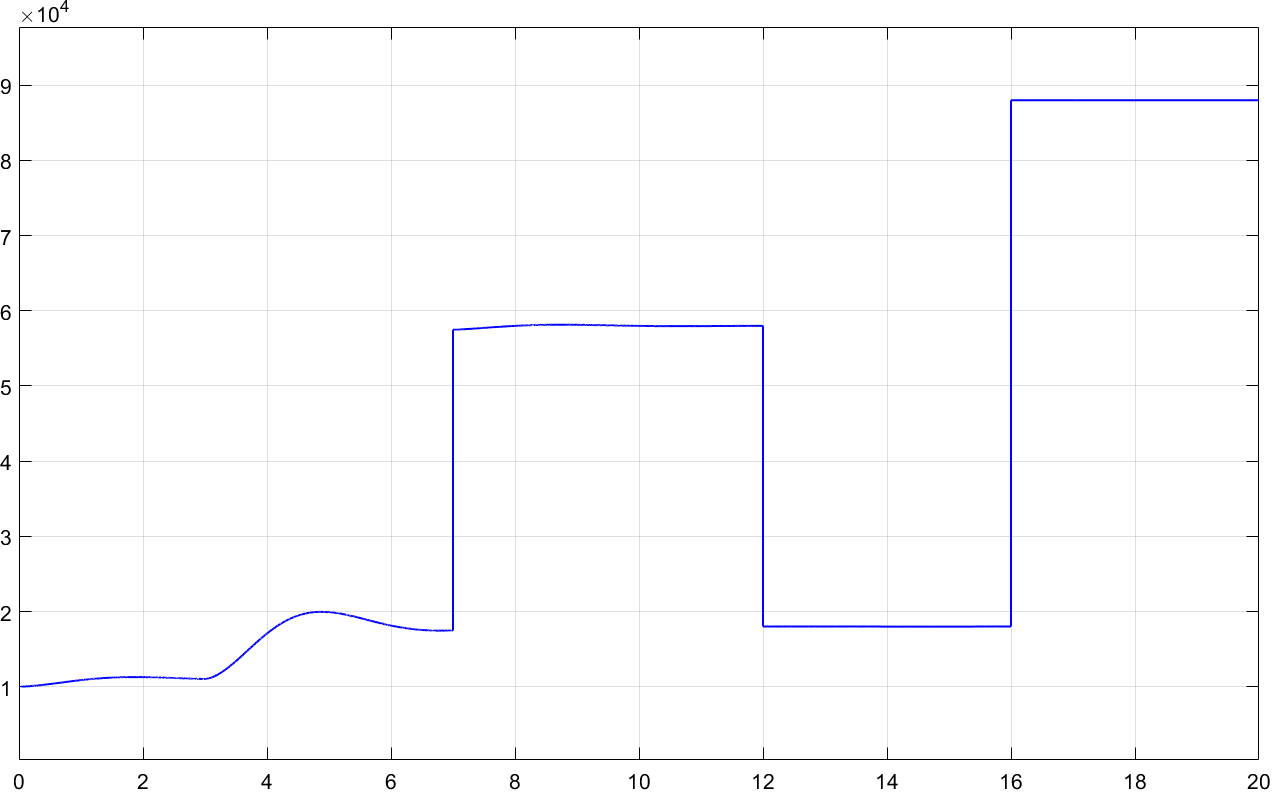
\includegraphics[width=1\textwidth]{rapport/billeder/temporary/load_power}
\caption{Load characteristics for the simulation in power.}
\label{fig:load_power}
\end{figure}

 In \figref{fig:voltage_dist}, the disturbance in the output voltage, caused by the change in load, can be seen.

\begin{figure}[H]
\centering
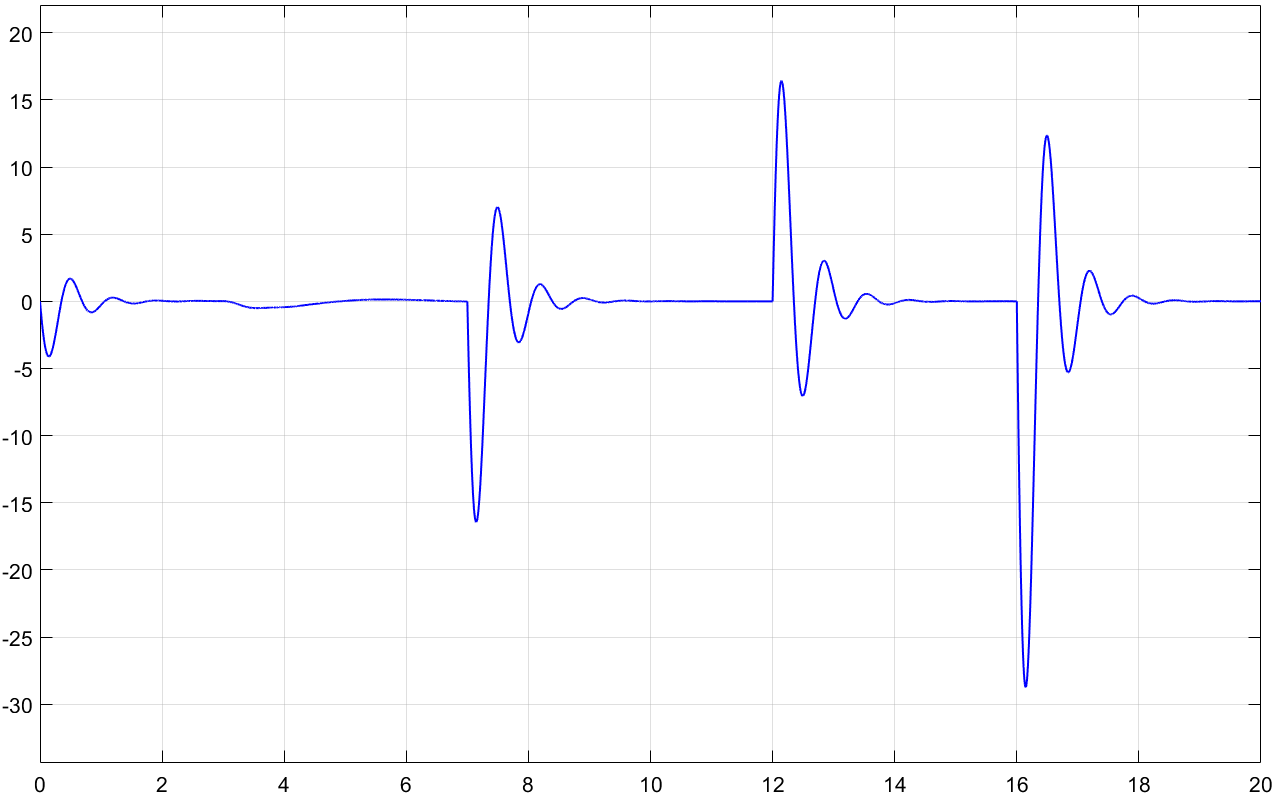
\includegraphics[width=1\textwidth]{rapport/billeder/temporary/load_voltage}
\caption{Voltage disturbance due to changes in the load.}
\label{fig:voltage_dist}
\end{figure}

In \figref{fig:state1} the comparison between the original and the estimated value for the first state can be seen.

\begin{figure}[H]
\centering
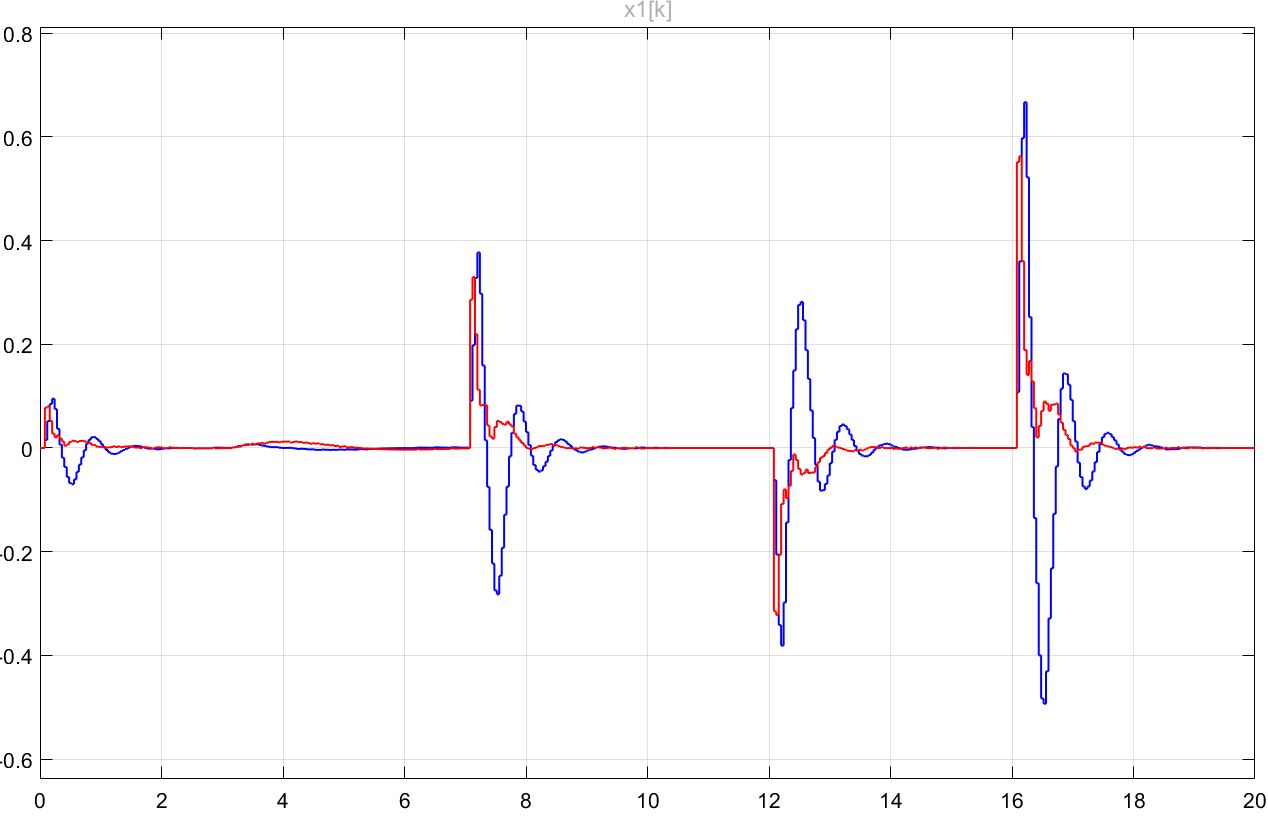
\includegraphics[width=1\textwidth]{rapport/billeder/temporary/state1}
\caption{Comparison of original and estimated value for the first state.}
\label{fig:state1}
\end{figure}

The same comparison for the second state can be seen in \figref{fig:state2}: 

\begin{figure}[H]
\centering
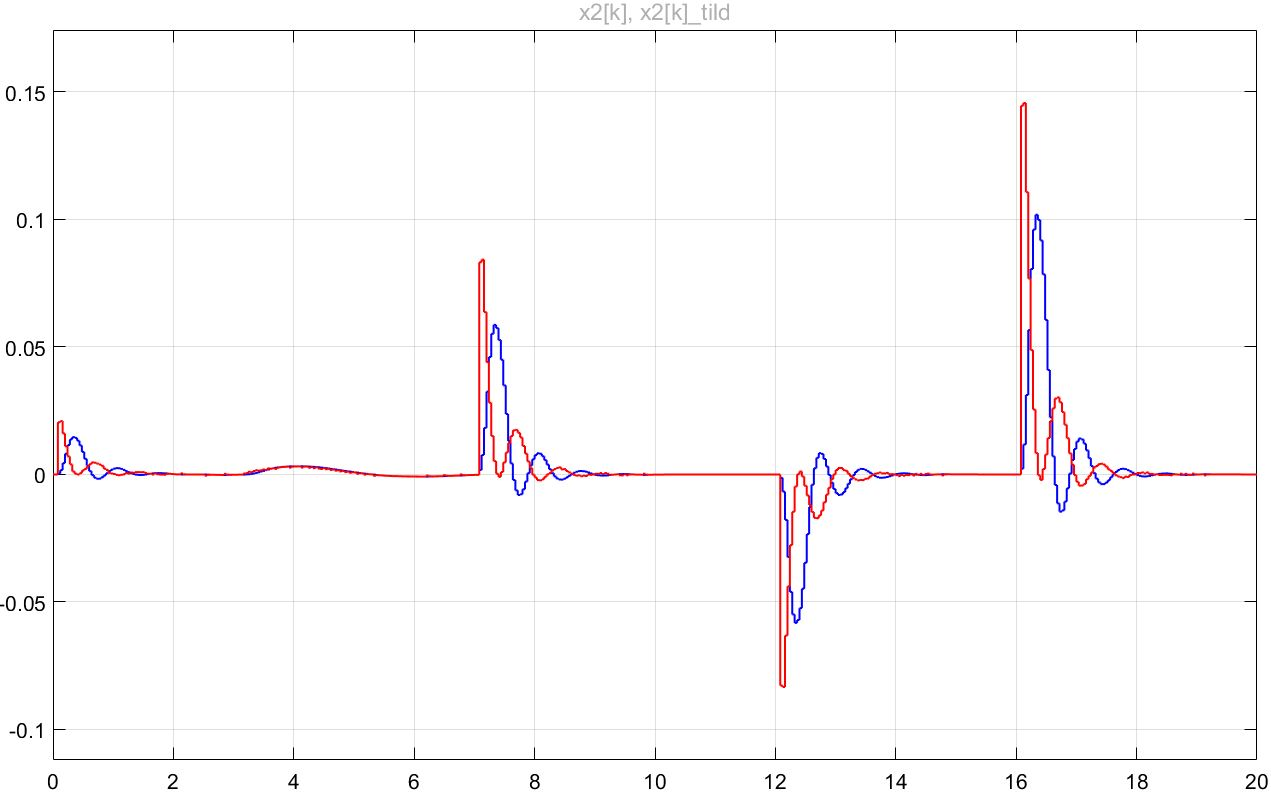
\includegraphics[width=1\textwidth]{rapport/billeder/temporary/state2}
\caption{Comparison of original and estimated value for the second state.}
\label{fig:state2}
\end{figure}

In \figref{fig:errorzero} the size of the error signal is shown.

\begin{figure}[H]
\centering
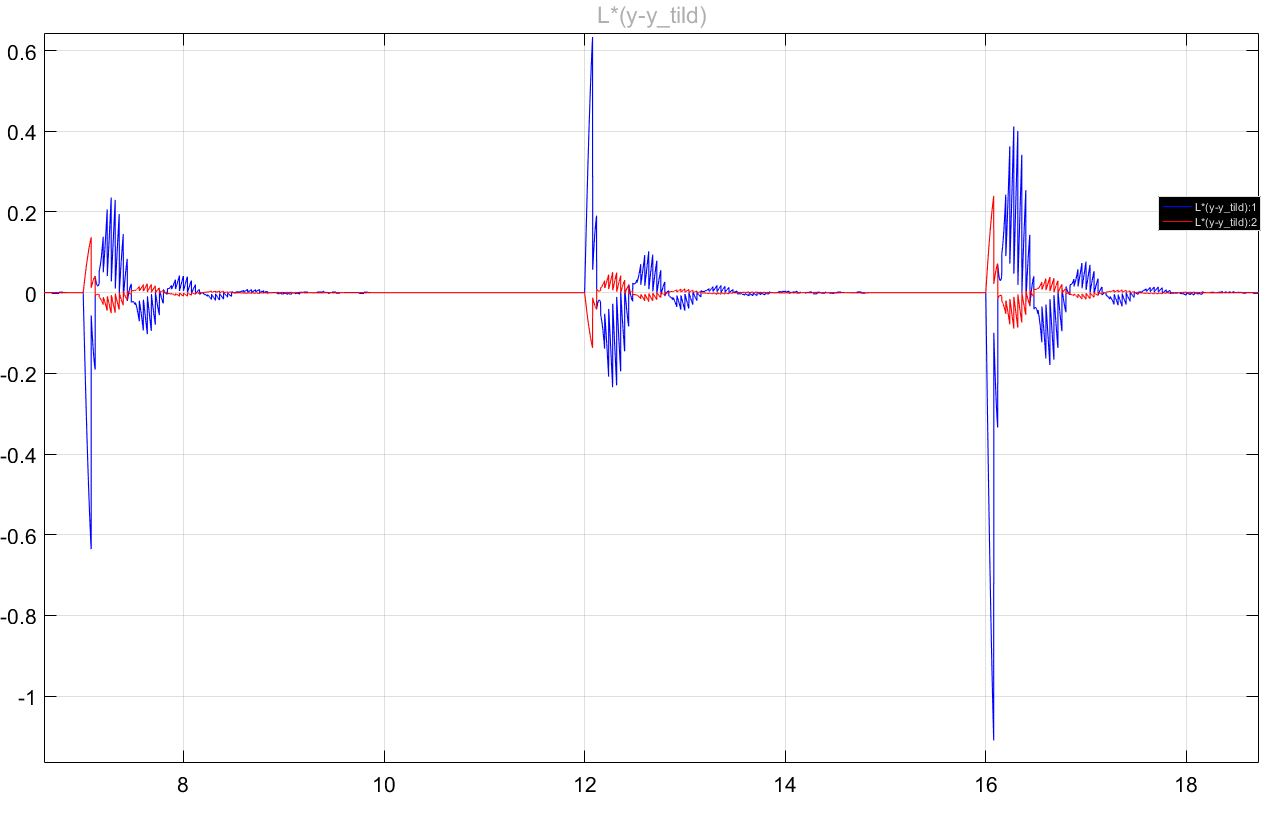
\includegraphics[width=1\textwidth]{rapport/billeder/temporary/errortozero}
\caption{Dynamics of the estimation error.}
\label{fig:errorzero}
\end{figure}

While in \figref{fig:est_out} the estimate of the output is shown. 

\begin{figure}[H]
\centering
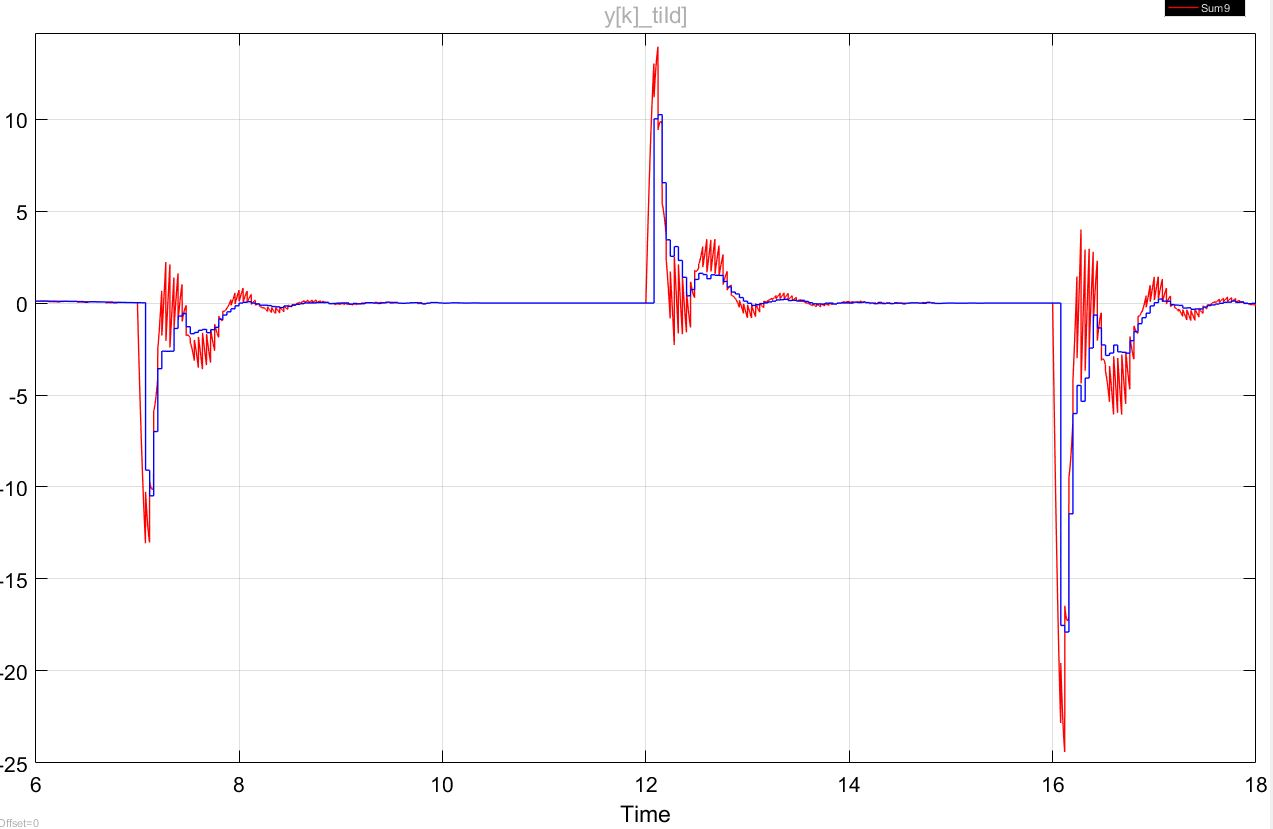
\includegraphics[width=1\textwidth]{rapport/billeder/temporary/outputcomparison}
\caption{Graph showing how the output follows the original output.}
\label{fig:est_out}
\end{figure}
\chapter{Simulation}\label{ch:simulation}
In this chapter the schemes utillized to be able to simulate the non linear parts of the sewage flow with its various concentrations is explained.



%\chapter{Network}
%\section{CAN bus}
\label{sec:Canbus}

Communication between the genset controller and the genset is done via Controller Area Network (CAN) bus. The controller developed in section() which handles the genset frequency, is effectively changing the fuel quantity to the diesel engine. Due to this the communication has to be between the designed controller and the internal engine control.

The CAN bus communication is a type of field bus original designed for use in vehicles and commonly used for control purposed between motors and motor controller. Comparing CAN bus to the open system interconnection (OSI) model the CAN bus consists of three layers. The physical, the data link and the application layer. The lower layers as the physical and data link layers are described in the ISO 11898 standard \cite{CAN_whitepaper_NI}. 

For the physical layer there are generally three different options, a two wire high speed bus that is capable of speeds up to 1Mbit/s when the distance is under 40 meters. Furthermore another two wire option described in ISO 11898-3 is available, this is a low speed fault tolerant version, where the speed is 125kbit/s. The last option is a single wire bus where the speed is limited to 33,3 kbit/s or 83,3 kbit/s in diagnostic mode, this is described in SAE J2411 \cite{CAN_singlewire}.
The logic levels are also specified in these standards. For a two wire CAN bus, a logical 0 corresponds to a high voltage differential between the two communication wires and a logical 1 corresponds to a low voltage differential between the communication wires. This is shown on \figref{fig:CAN_voltage}. 

\begin{figure}[H]
\centering
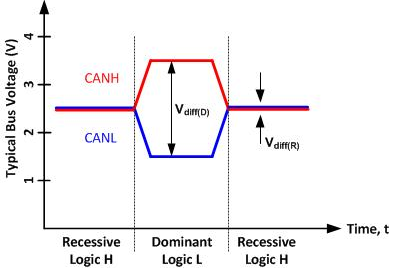
\includegraphics[width=0.75\textwidth]{rapport/billeder/CAN_voltage}
\caption{Voltage levels on a two wire CAN bus \cite{fig_CAN_V_levels}.}
\label{fig:CAN_voltage}
\end{figure}     
%https://e2e.ti.com/blogs_/b/industrial_strength/archive/2015/06/04/what-do-can-bus-signals-look-like
For a single wire CAN bus according to SAE J2411 the recessive and dominant logical values will behave the same, but the voltage differential will be according to ground. 

Concerning the CAN data link layer this can be divided into classical CAN and a new version with flexible data rate called CAN FD, both are described in ISO 11898-1. 
The data link layer will be described for classical CAN, however CAN FD uses the same structure and is therefor backwards compatible if a classical CAN frame is received.

The layout of frames on the CAN bus follow the structure of \figref{fig:CAN_frame}.

\begin{figure}[H]
\centering
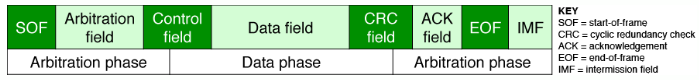
\includegraphics[width=0.75\textwidth]{rapport/billeder/CAN_frame}
\caption{Showing the layout of a CAN bus data frame \cite{fig_CAN_frame}.}
\label{fig:CAN_frame}
\end{figure}

On \figref{fig:CAN_frame} a general CAN bus frame is showed, where SOF is the start-of-frame field. The arbitration field contains an ID of either 11 or 29 bytes and determines the priority where a lower ID yields a higher priority. The control field contains informations about data length and type. The data field contains the actual data which for classical CAN is up to 8 bits and for CAN FD up to 64 bytes. After the data field a 15 bit cyclic redundancy check (CRC) field is present. This is followed by an acknowledgment (ACK) field where nodes that received the message will send an ACK and the transmitting node will listen and either retransmit the data if no ACK is present or end the frame if an ACK is received. This is the general frame structure for CAN bus.   


Depending on the settings of the frame four different message types are available on the CAN bus. 
The frame shown on \figref{fig:CAN_frame} is an example of a data frame, which purpose is to transmit recorded data over the bus. Another frame type is a remote frame which has no data and a specific bit set in the control field to specify it is a remote frame. The purpose of this frame is to request a data frame form other nodes. The last two message types are error frames and overload frames, where the error frame consists of a six bit error flag and an eight bit error delimiter. The structure of the overload frame is similar.  

The CAN bus is structured without a master, instead all nodes are broadcasting to every one else. This implies that transmitting data to a specific node is impossible, as everyone is listening and the message is transmitted on the entire bus. In order for a node to transmit on the bus, it checks if the bus is free and if that is the case it transmits. This structure can results in message collisions as two nodes both waiting for the bus to become free will start transmitting at the same time. In order to solve this and select which note should transmit, the arbitration field is used, where the node with the lowest ID wins. This behavior is due to the dominant property of logital 0 which naturally favors lower arbitration ID's, this can be seen on \figref{fig:CAN_arbitration}.  

\begin{figure}[H]
\centering
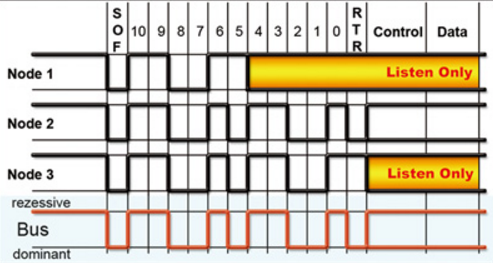
\includegraphics[width=0.75\textwidth]{rapport/billeder/CAN_arbitration}
\caption{Showing arbitration behavior on a CAN bus \cite{fig_CAN_arbitation}.}
\label{fig:CAN_arbitration}
\end{figure}
%http://www.icpdas.com/root/product/solutions/industrial_communication/fieldbus/can_bus/can_intro.html

A communication example of three nodes on a CAN bus network is shown on \figref{fig:CAN_arbitration}. Here the transmitted signals from the nodes is shown in black and the signal on the CAN bus is shown in red. The example shows that when node one tries to transmit a logical 1 as the other nodes transmit a logical 0 node one will lose arbitration as logical 1 is recessive. After this, node one will only listen to the bus and wait until it is not occupied. The example also shows that node 3 looses arbitration at the RTR field, which determines weather the frame is a data or remote frame. A remote frame has RTR set as recessive, therefore data frames are prioritized higher than remote frames in CAN bus and node two wins arbitration.   



%\begin{figure}[H]
%\centering
%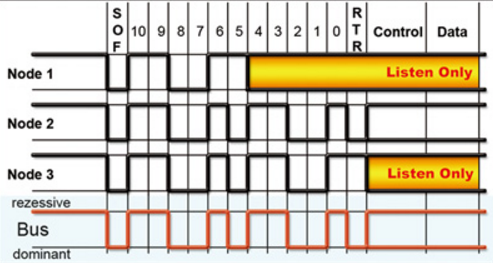
\includegraphics[width=0.75\textwidth]{rapport/billeder/CAN_arbitration}
%\caption{.}
%\label{fig:blok}
%\end{figure}

%1* highspeed can, 2 wires, up to 1Mbit/s  ISO 11898-2
%2* Lowspeed can (fault tolerant), 2 wires,  up to 125 kbit/s 11898-3
%3* Single wire can, 33,3 kbit/s or 83,3 kbit/s in high-speed diagnistics mode, 

%1*
%http://digital.ni.com/public.nsf/allkb/84210794086E9C0886256C1C006BE6AE



%2*
%http://digital.ni.com/public.nsf/allkb/84210794086E9C0886256C1C006BE6AE



%3*
%SAE J2411 (https://www.can-cia.org/can-knowledge/can/sae-j2411-single-wire/)


%alle
%https://www.kvaser.com/can-protocol-tutorial/
%http://www.ni.com/white-paper/2732/en/

%CAN FD
%https://www.kvaser.com/about-can/can-fd/



%\section{dSPACE Unit}

A dSPACE unit is a multipurpose unit for implementing and testing controllers. The provided dSPACE unit contains a DS1103 PCC controller board.  % https://www.dspace.com/en/inc/home/products/hw/singbord/ppcconbo.cfm
The dSPACE unit is a platform that makes it possible to implement a control directly from simulink to the test plant. This is smart because almost every control engineering controller is designed without simulation, and therefor the controller is already implemented in simulink. This is also the case is this project. 

The provided dSPACE controller board is made for general motor control. The unit is fitted with both digital I/O, A/D converters, D/A converters and a CAN interface which is often used in motor applications, and also for the provided genset. 


\subsection{Implementation}
\label{dspace_unitv2}
% Opbygning start med at vise, hvad det er vi bruger hardware. Vis billeder også gå ind i software og beskriv bloggene 

This subsection will elaborate how to implement the controller on the dSPACE unit. Furthermore the software tool ControlDesk will be explained. 

As elaborated previously the controller will be implemented in simulink. To control the references for the AVR and governor through simulink a system block, which have been designed by dSPACE Real-Time Interface (RTI) \cite{dSPACE_software}, have been used. This block allows the user to send references to the AVR and governor through CAN bus. These system blocks are illustrated in \figref{fig:can_setup}:

\begin{figure}[H]
\centering
\includegraphics[width=1\textwidth]{rapport/billeder/cansetup}
\caption{System blocks for setting up CAN connection to the genset for voltage and frequency.}
\label{fig:can_setup}
\end{figure}    

The top module is used to set the frequency reference and the bottom is used to set voltage reference. The block called speed is used to set the wanted frequency in Hz for the output of the genset. To set the reference for voltage the block actVOLTAGE needs to be set at the desired output. The rest of the blocks are determent by the genset and the values can be found in the datasheet for the genset that will be tested on. 

To calculate the output in frequency and voltage, calculations done in simulink by Jesper Viese Knudsen, have been used. In \figref{fig:RMS_for_onePhase_simulink} it is illustrated how to calculated RMS voltage for one phase. 

\begin{figure}[H]
\centering
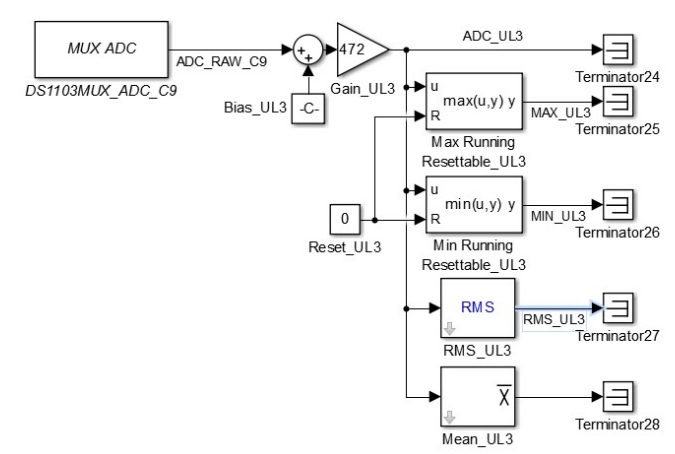
\includegraphics[width=0.8\textwidth]{rapport/billeder/RMS_for_onePhase_simulink}
\caption{System blocks for calculating RMS voltage for one phase.}
\label{fig:RMS_for_onePhase_simulink}
\end{figure} 

The output of block RMS\_UL3 will be used to calculate one phase of the voltage. The output will be in rms voltage, and to calculate all three phases, three setups like the on in \figref{fig:RMS_for_onePhase_simulink} will be used. 

In \figref{fig:CAN_frequency} an illustration of the system blocks to calculate frequency is shown. 

\begin{figure}[H]
\centering
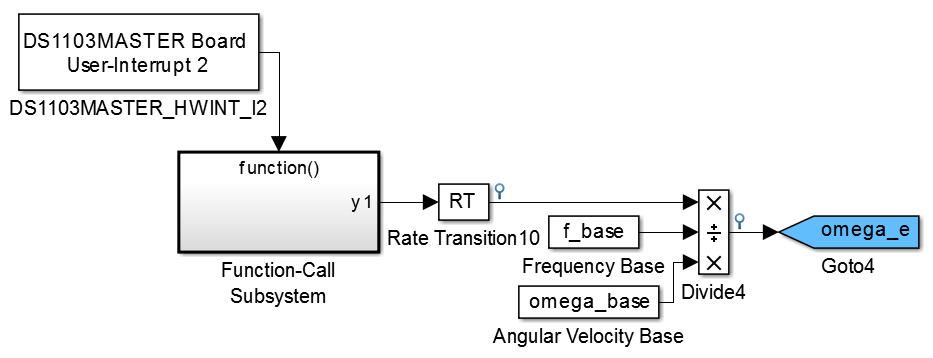
\includegraphics[width=0.8\textwidth]{rapport/billeder/CAN_frequency}
\caption{System blocks for calculating frequency.}
\label{fig:CAN_frequency}
\end{figure} 

The output of Divide4 is the frequency in rad/s which will be used to see if the frequency of the genset is stable with the controller designed in \secref{system_design_implementation}. 
It calculates the frequency through an sfunction in matlab, which uses interrupts from the tachometer placed inside the engine, to generate an input to this sfunction. By that a output in frequency will be calculated. 


These blocks have been added together with the controller designed in \secref{system_design_implementation} and the full implementation is illustrated in \figref{fig:full_implementation}.
\begin{figure}[H]
\centering
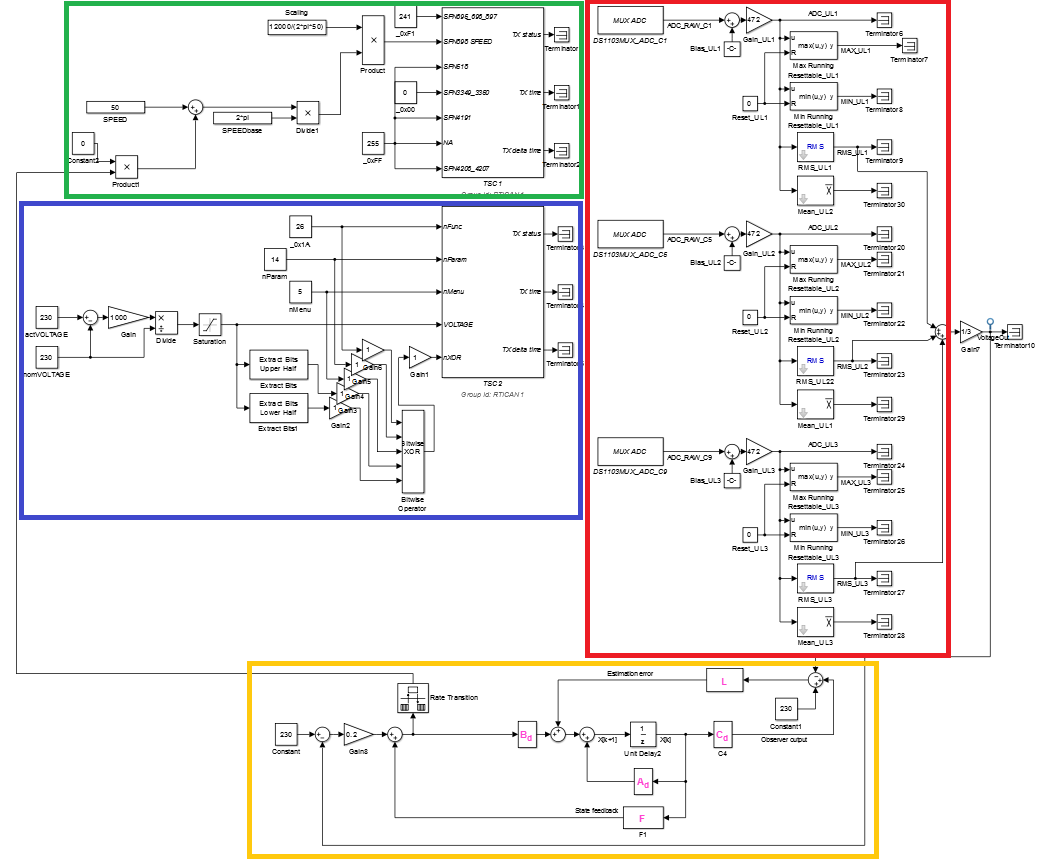
\includegraphics[width=1.1\textwidth]{rapport/billeder/full_implementation}
\caption{Full implementation on the dSPACE unit. In the green box the transformation from frequency reference to CAN bus commando for the governor is made. In the blue box the transformation from voltage reference to CAN bus commando for the AVR is made. The red box is transformation to RMS voltage. The yellow box is the controller.}
\label{fig:full_implementation}
\end{figure} 

To compile the simulink file the following code needs to be runned in matlab:

\begin{lstlisting}
rti_build('CA7_full_system')
\end{lstlisting}

When it has compiled it will be uploaded to the dSPACE unit. 

To analyses the output of the blocks in \figref{fig:full_implementation} ControlDesk have been used. ControlDesk is a software used to measure realtime data and gives the possibility to change values realtime. In this project it has been used to adjust the gain to find the parameter that fits the genset the most as in \secref{app:controller_test} Furthermore it has been used to track the output frequency and voltage, the states of the observer and the output of the observer. This gives the possibility to investigate if the values, an example is to look at the states of the observer to see if they are going towards infinity or towards zero which makes the search for error faster. 

 
% Furthermore the hardware that will used in this project will be shown and described.  

% The dSPACE unit is connected to a PC that runs simulink, matlab and ControlDesk these software tools will be elaborate later in this subsection. Furthermore, it is connected to several boards that are mounted on a wooden plate. These boards enable the dSPACE unit to measure voltage and current, communicate over CANbus and use calculated the electric frequency of the genset.  

% \begin{figure}[H]
% \centering
% \begin{subfigure}{.5\textwidth}
%   \centering
%   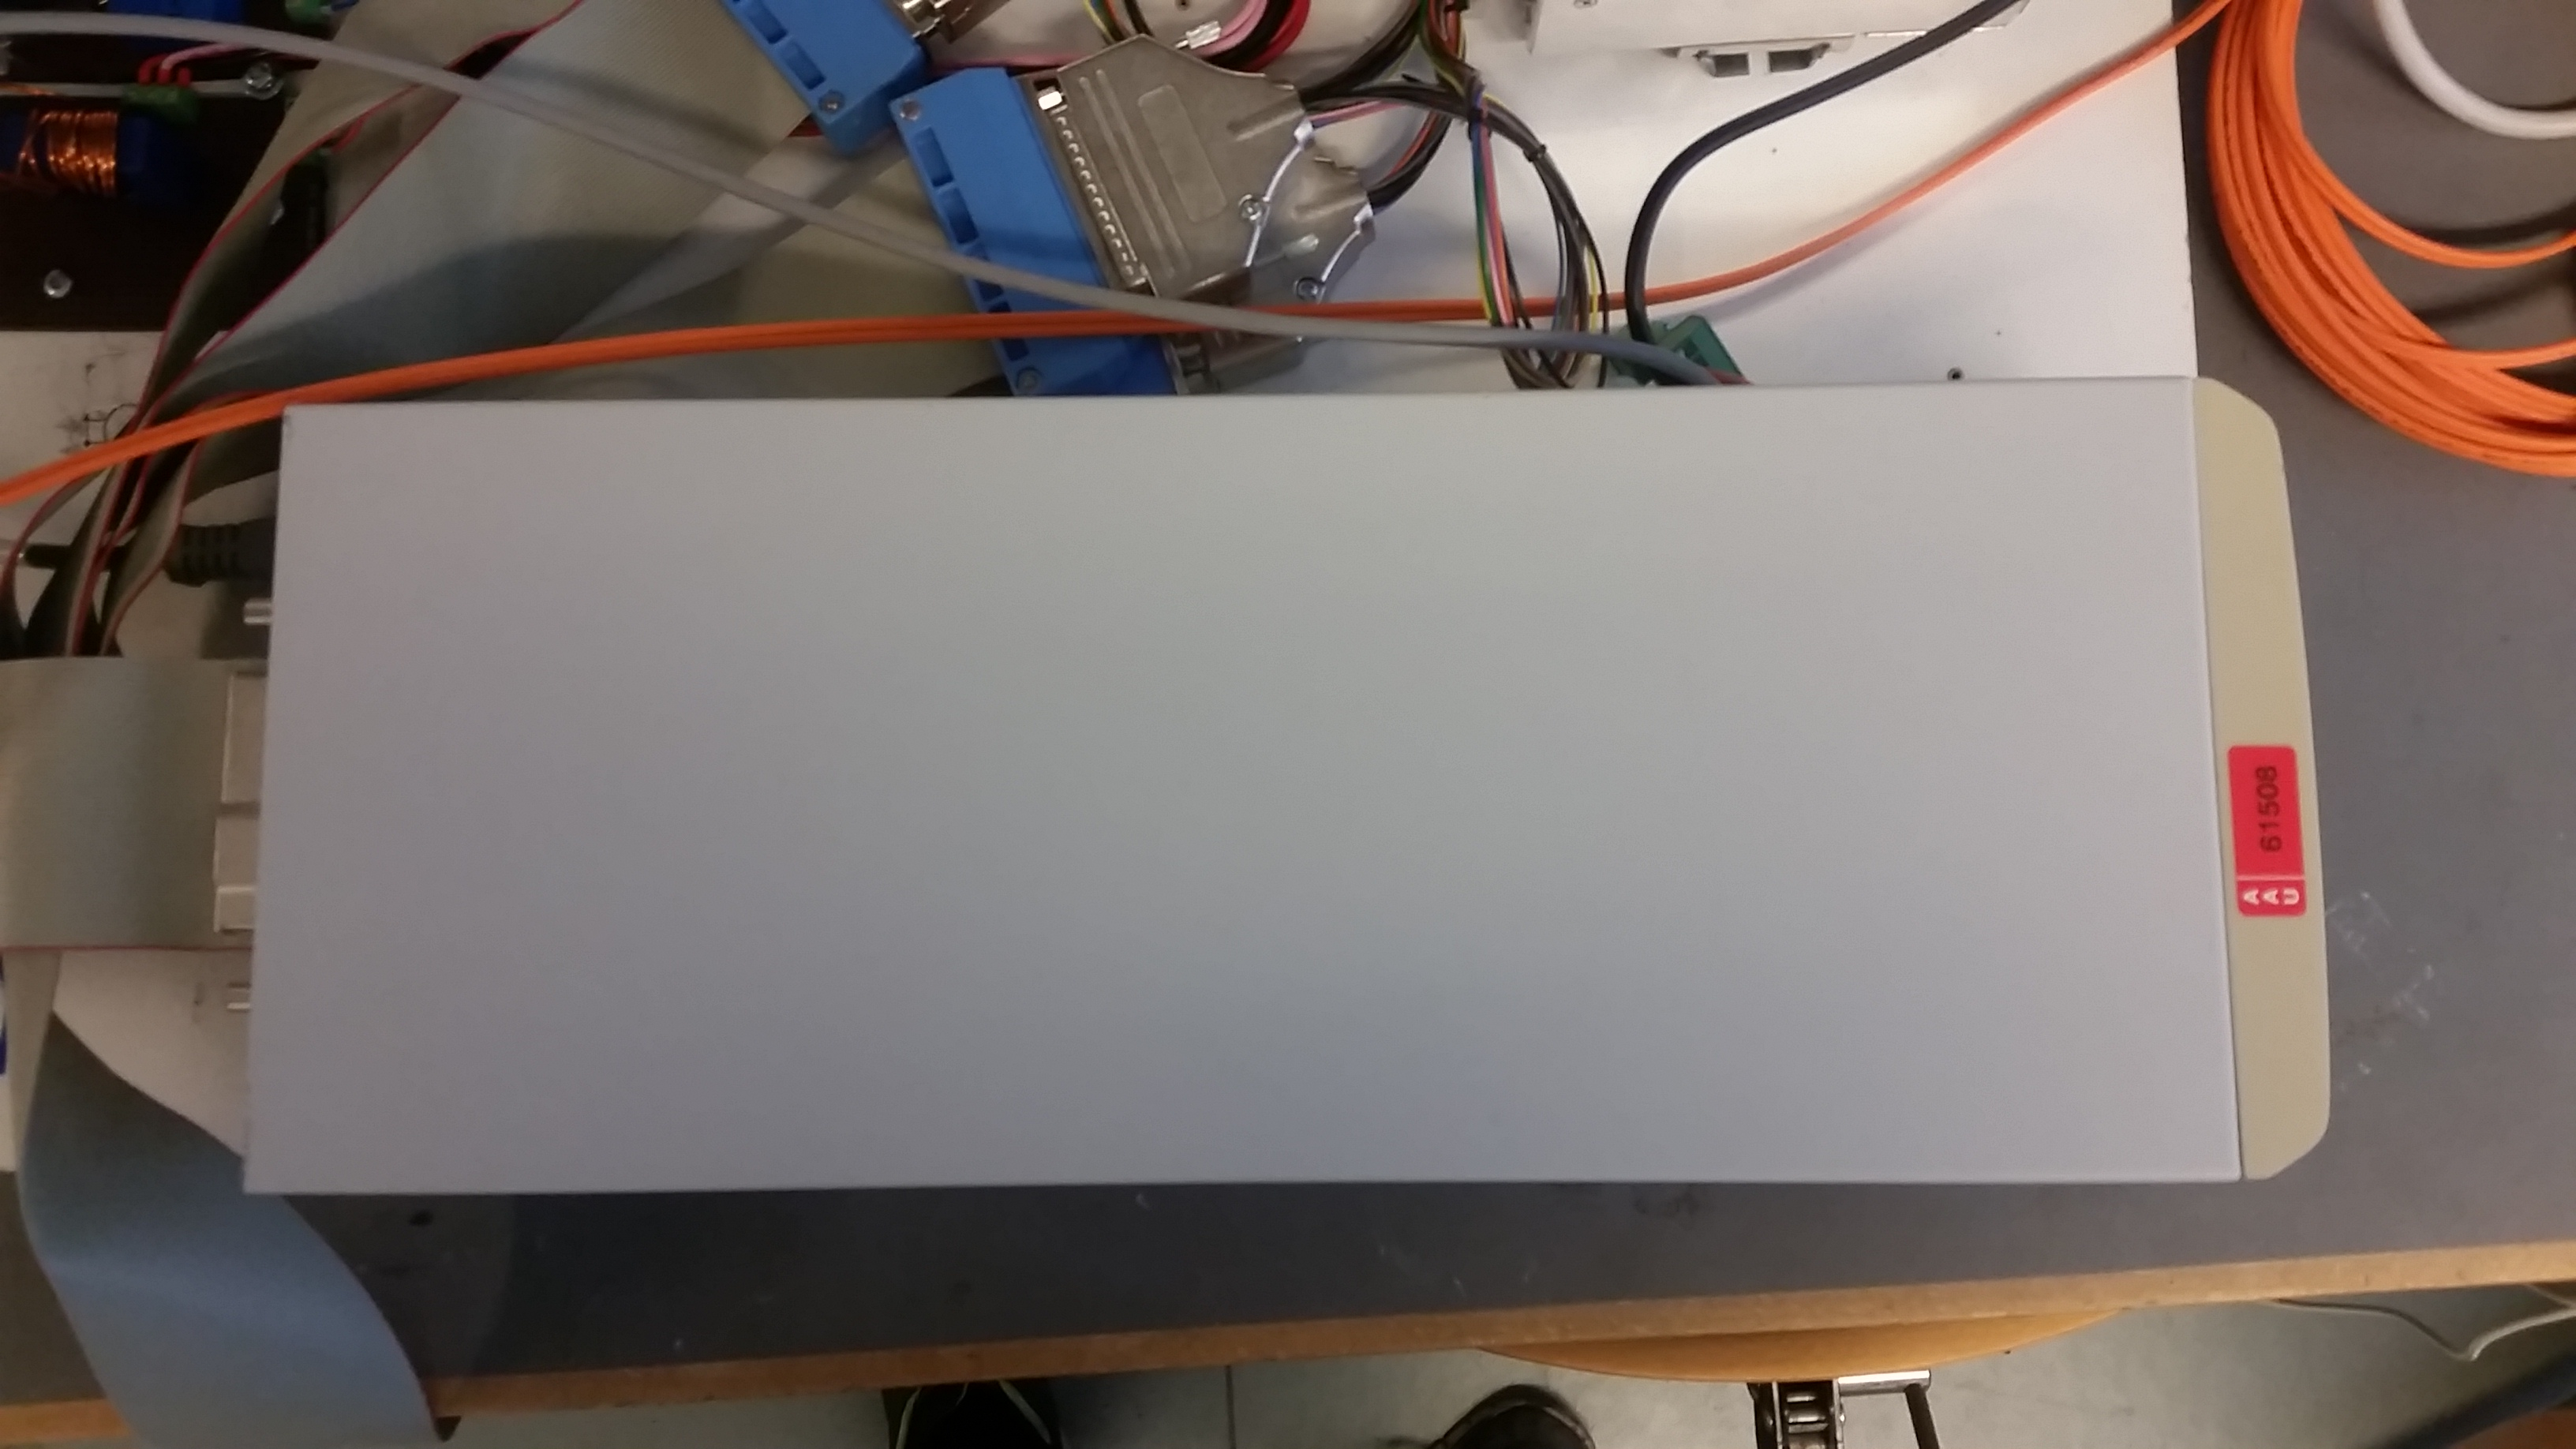
\includegraphics[width=0.75\textwidth]{rapport/billeder/dspace_unit}
%   \caption{}
% \end{subfigure}%
% \begin{subfigure}{.25\textwidth}
%   \centering
%   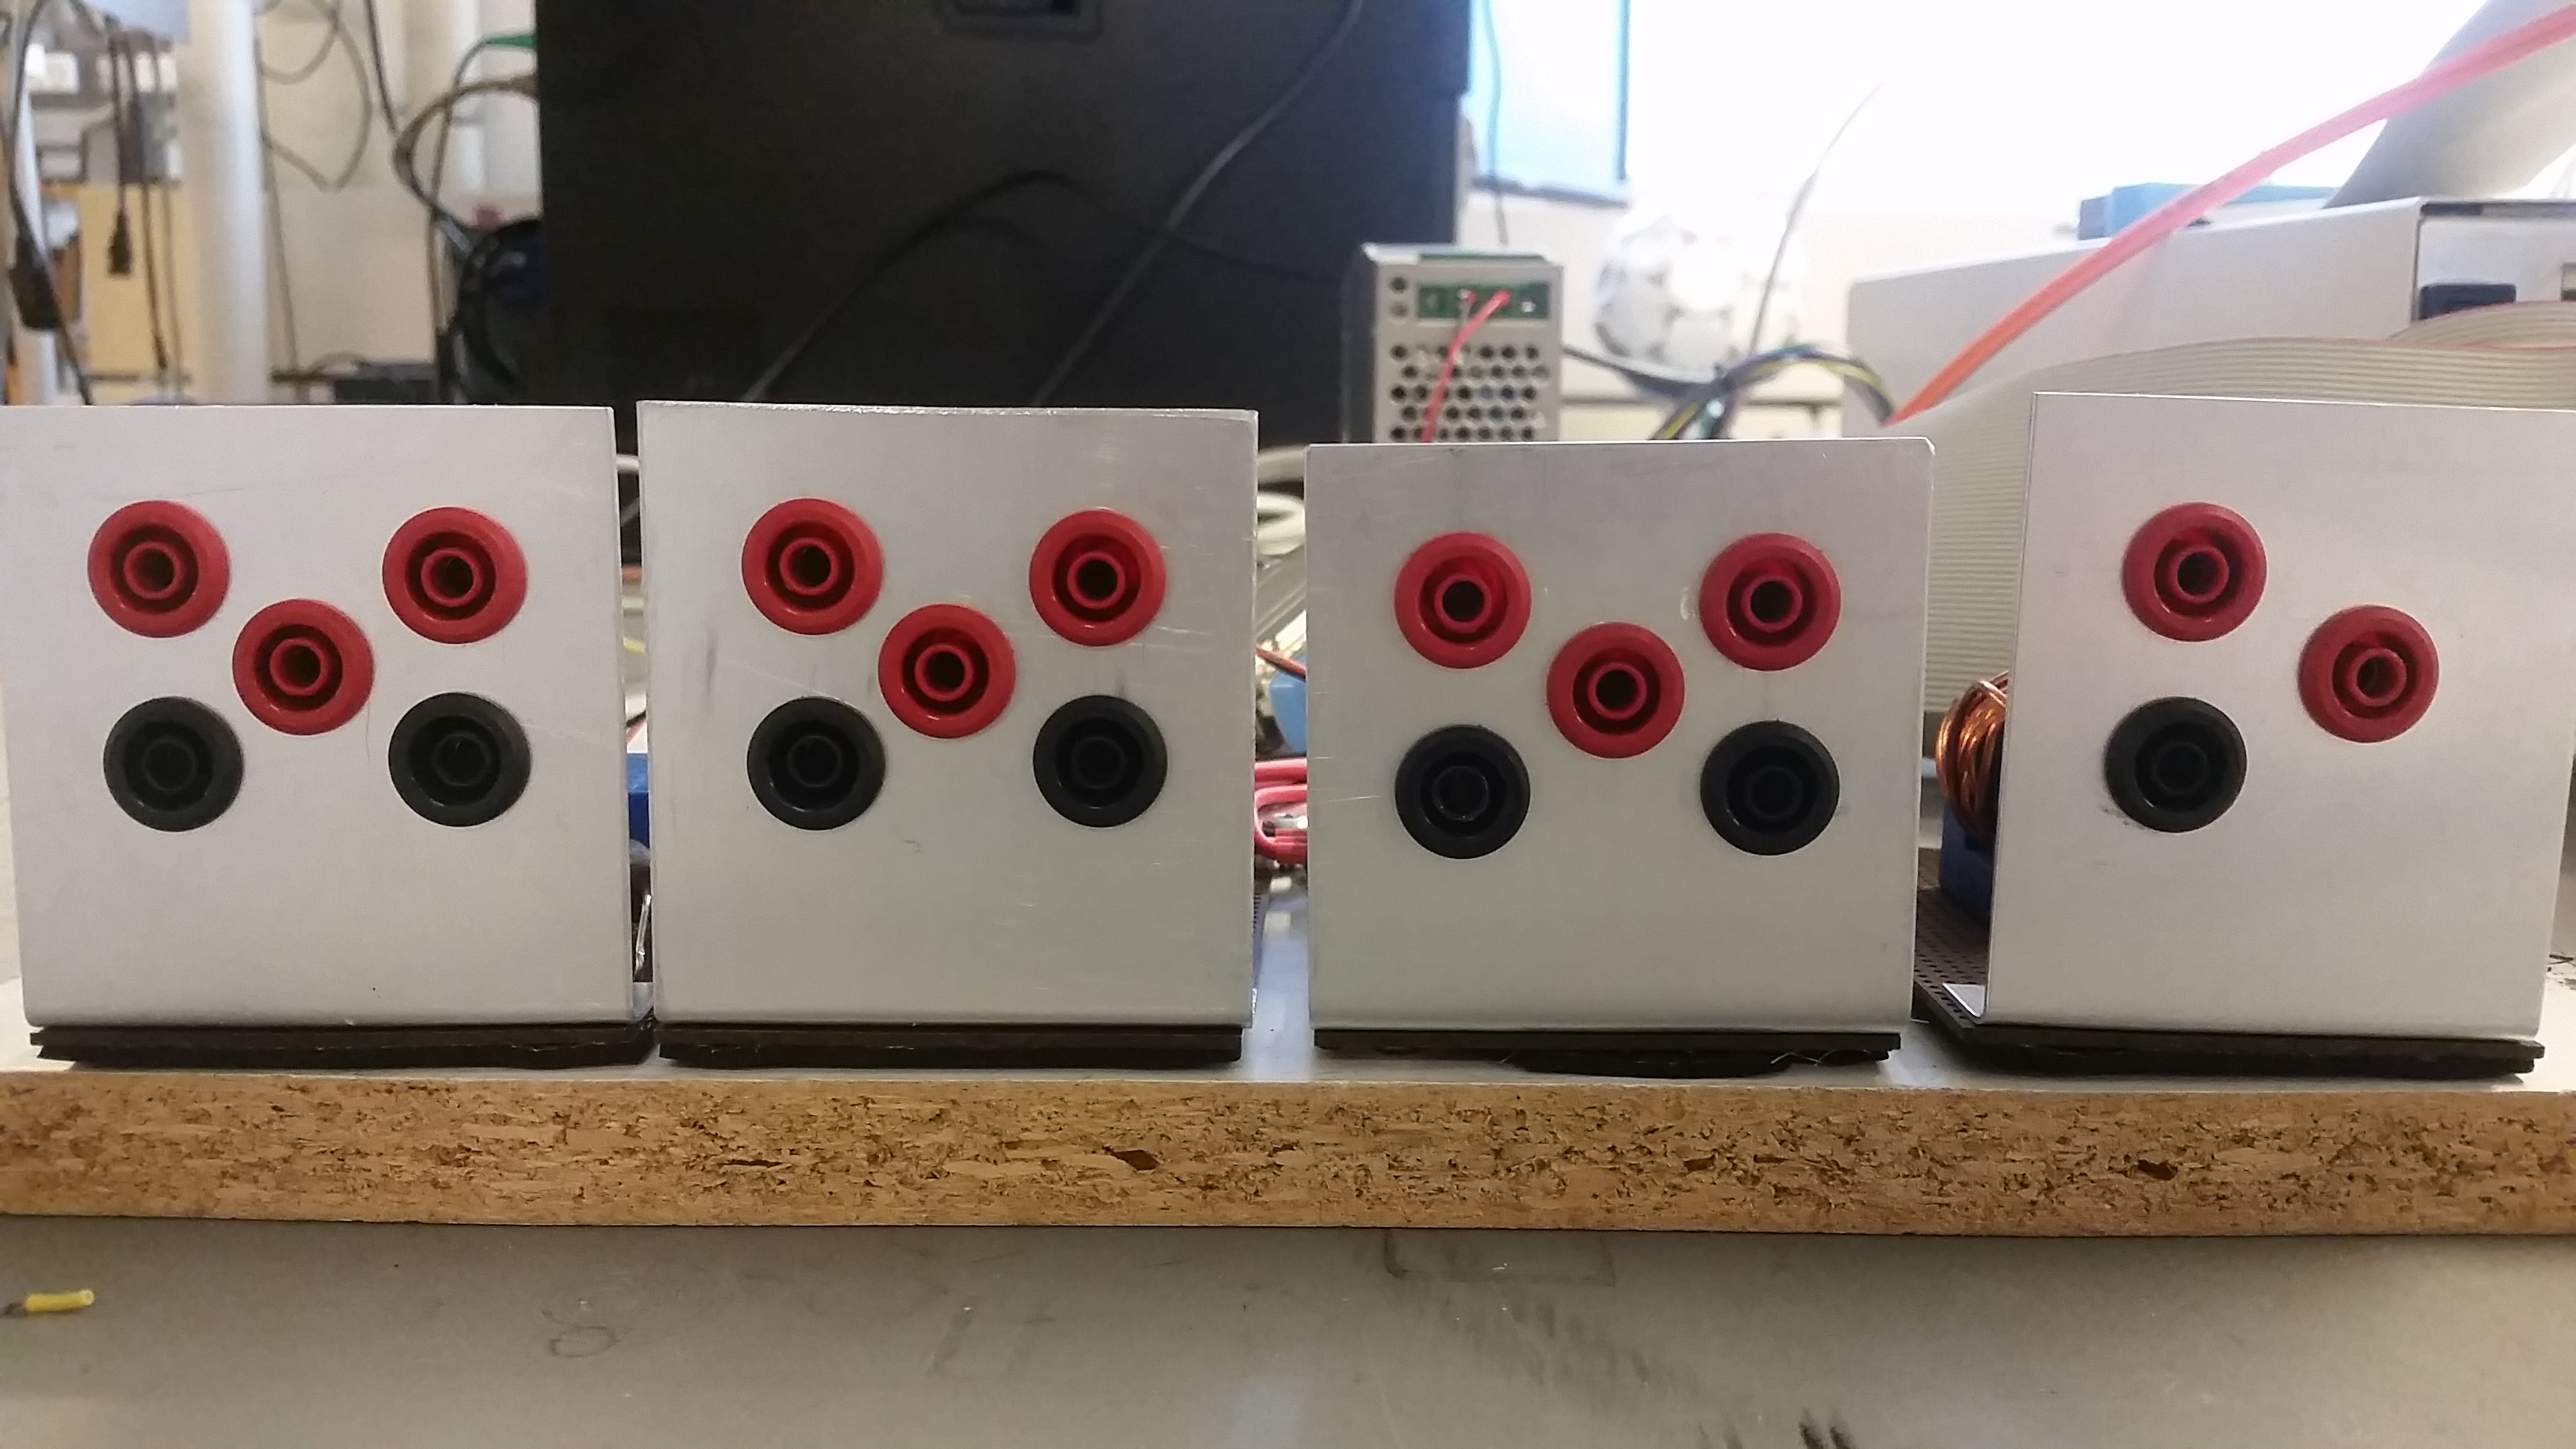
\includegraphics[width=1.5\textwidth]{rapport/billeder/Voltage_Current}
%   \caption{}
% \end{subfigure}
% \caption{(a) The dSPACE unit. (b) Voltage and current measurement inputs.   }
% \label{fig:dspace_voltage_current}
% \end{figure}

% On the backside of the dSPACE unit, there is placed the connections for communication with PC and the connection to all the boards that are placed on the wooden plate. In \figref{fig:dspace_voltage_current} b the voltage and current measurements inputs are shown. There are placed four current measurements which is able to measure current from ?? to ?? and from ?? to ?? \fxnote{Hear Jesper what the size of the current measurement}. It is also able to measure three different voltage signals. 

% \begin{figure}[H]
% \centering
% 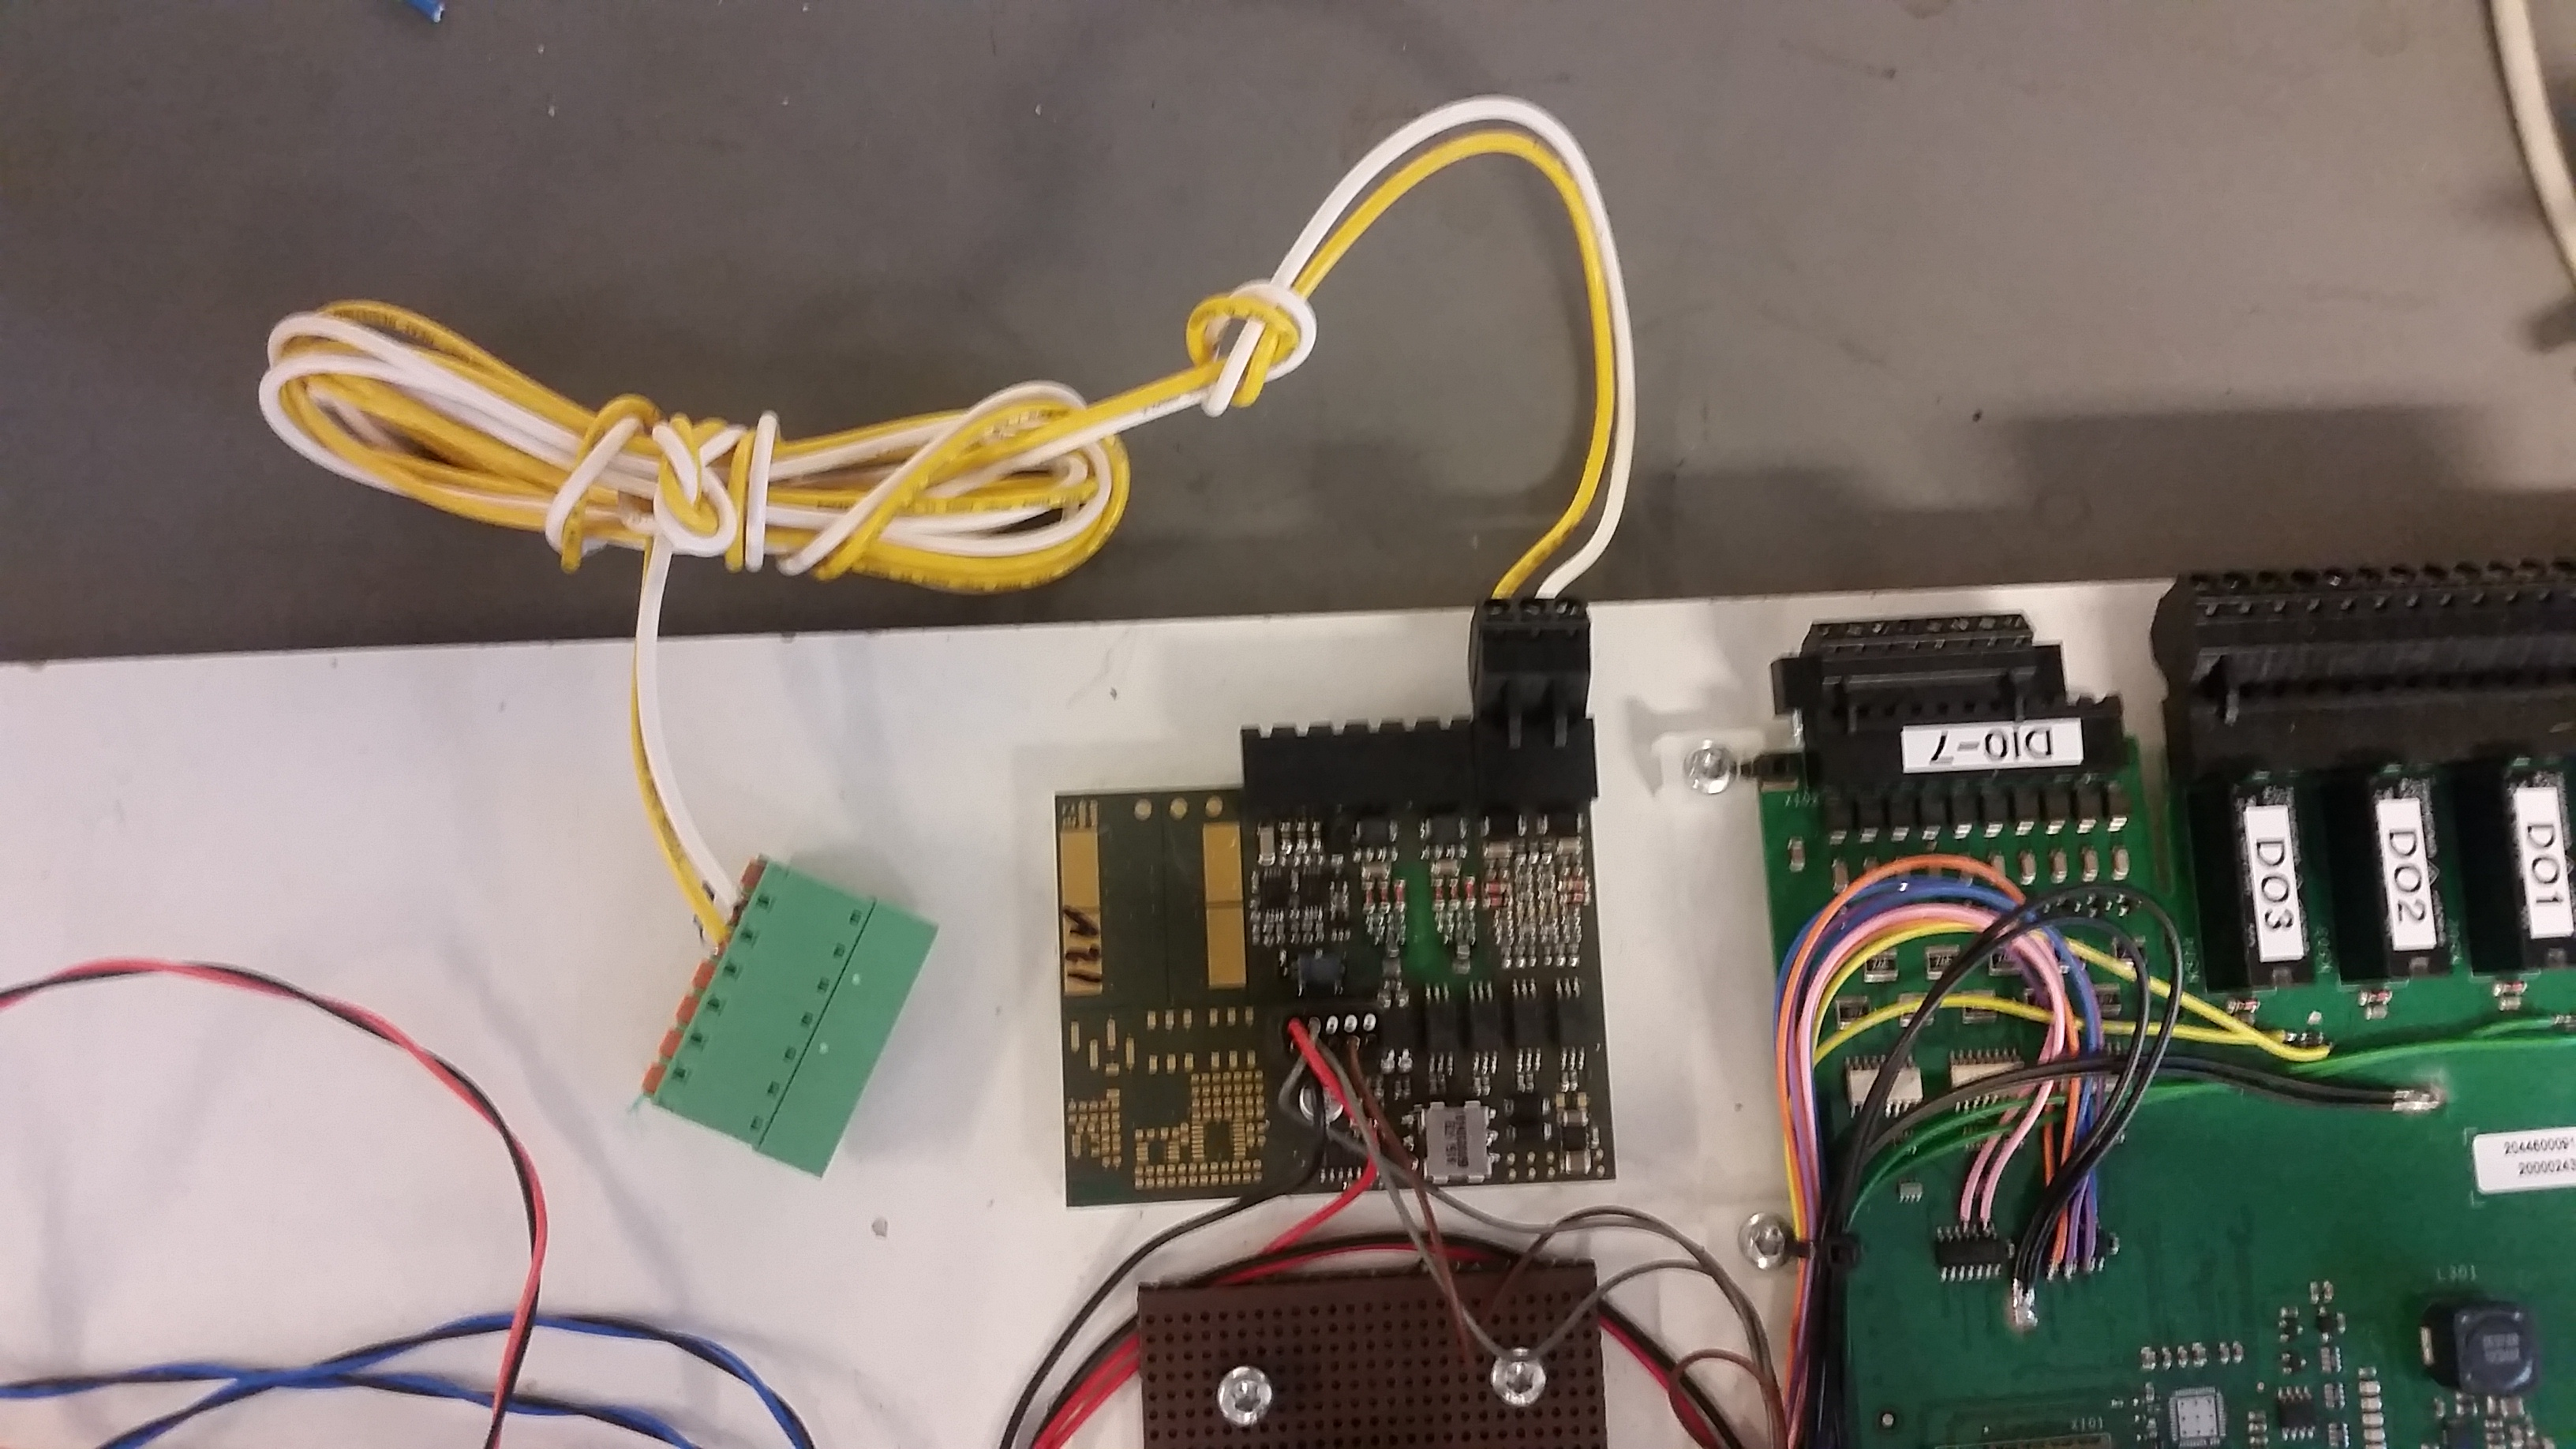
\includegraphics[width=0.50\textwidth]{rapport/billeder/frequence_interrupt}
% \caption{For measuring frequency.}
% \label{fig:CAN_arbitration}
% \end{figure}    

% \fxnote{Need something to call this board} This board is able to receive interrupts from the the genset, which can be used to calculated the electric frequency. I need to elaborate this. (Jacob)

% To implement the controller, simulink is used with a dSPACE toolbox.  

% Something on the overall system like the compelete setup with computer and wooden board

% Break down in smaller piceses(stykker) start with the board 

% Go into the simulink files

% End with the matlab file

% Maybe our controller implemented in simulink. 

% \begin{figure}[H]
% \centering
% 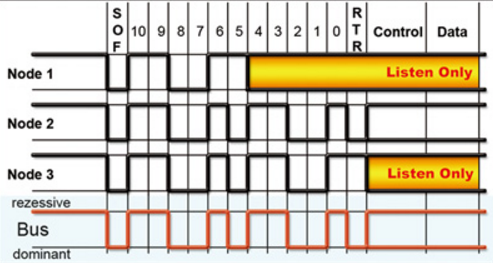
\includegraphics[width=0.75\textwidth]{rapport/billeder/CAN_arbitration}
% \caption{Showing arbitration behavior on a CAN bus \cite{fig_CAN_arbitation}.}
% \label{fig:CAN_arbitration}
% \end{figure}

\chapter{Results}
\input{rapport/design/Results}


% %Accepttest 
% %\part{ Conclusion and verification}
%\label{conclusion_and_verification}

\chapter{Accepttest}
\label{accepttest}


% %\bfseries
% \begin{table}[H]\hspace*{-1cm}
% \centering
% \begin{tabular}{|c|c|c|c|c|c|} \hline
% \rowcolor{lightgray}  Req. no. 	& \bfseries Requirement 					&  \bfseries Reference											&\bfseries Result   &\bfseries Fulfilled\\ 
% \rowcolor{lightgray}			&											&  																&					&	 				\\ \hline
	
% 	& &  							&  & $\surd$			\\ 
%  								& 				& 			&	 				&					\\ \hline
% %
% 	& &  						& 	& $\surd$			\\ 
% 								& & &					&					\\ \hline
% %
% 	& & & & $\times$	\\ 
% 								& 						& &					&					\\ \hline
% %
% 	& & & & $\times$		\\ 
% 								& 						& &					&					\\ \hline
% %									
% 	& & & & $\surd$		\\ 
% 								& 	 				&& 				&					\\ \hline
% %
% 	& & 		& & $\times$	\\ 
% 								& 						& 		 						&					&					\\ \hline
% %
% 	& && & $\surd$		\\
% 								& 	& & 				&					\\ \hline
% \end{tabular}
% \caption{The fulfilment of requirements summarized.}	
% \label{table:accept_test_table}
% \end{table}


% \include{rapport/konklusion/Discussion}
% \chapter{Optimization}
\label{Optimization}
In this chapter a discussion upon what could be optimized to ease the scope of this project is made.


State feedback - Test with different poles placement of the state feedback

Network - include delay in controller

More test with the inverter to find the instability problem

Better model 

improve response of the AVR as it has been done for Governor. 



% % %Konklusion afsnit 
% \chapter{Conclusion}
\label{conclusion}


% %optimering/perspektiverings 
% %\chapter{Optimization}
%\label{optimering}


% %Bilag %

%Apendix
%%\part{Appendices}

\chapter{Appendix}



% \begin{figure}{.2\textwidth}
%   \centering
% 	\begin{tikzpicture}

\draw  [ultra thick](-3.5,3) node (v9) {} ellipse (8.5 and 8.5);
\node (v1) at (-12,13.5) {};
\node (v2) at (5,13.5) {};
\draw  [ultra thick](v1) edge (v2);

\node (v3) at (-11.5,14) {};
\node (v4) at (-11.5,13) {};
\draw  [ultra thick](v3) edge (v1);
\draw  [ultra thick](v1) edge (v4);
\node (v5) at (4.5,14) {};
\node (v6) at (4.5,13) {};
\draw  [ultra thick](v5) edge (v2);
\draw  [ultra thick](v6) edge (v2);
\node (v8) at (-10,-2.5) {};
\node (v7) at (3,-2.5) {};
\draw  [ultra thick](v7) edge (v8);
\draw  [ultra thick](v8) edge (v9);
\draw  [ultra thick](v9) edge (v7);


\node (v11) at (6,-5.5) {};
\node (v10) at (6,-2.5) {};
\node (v14) at (5.5,-3) {};
\node (v15) at (6.5,-3) {};
\node (v12) at (5.5,-5) {};
\node (v13) at (6.5,-5) {};
\draw  [ultra thick](v10) edge (v11);
\draw  [ultra thick](v11) edge (v12);
\draw  [ultra thick](v11) edge (v13);
\draw  [ultra thick](v14) edge (v10);
\draw  [ultra thick](v10) edge (v15);


\draw [ultra thick](-4.6491,2.0358) arc (-140.0003:-40:1.5);
\node (v16) at (-9.5,-6) {};
\node (v19) at (3,-6.5) {};
\node (v21) at (2.5,-6) {};
\node (v20) at (2.5,-7) {};
\node (v17) at (-10,-6.5) {};
\node (v18) at (-9.5,-7) {};
\draw  [ultra thick](v16) edge (v17);
\draw  [ultra thick](v18) edge (v17);
\draw  [ultra thick](v19) edge (v17);
\draw  [ultra thick](v20) edge (v19);
\draw  [ultra thick](v21) edge (v19);
\draw  [ultra thick](v8) edge (v7);
\draw  [ultra thick](v7) edge (v8);
\draw  [ultra thick](v8) edge (v7);
\draw  [ultra thick](v7) edge (v9);
\draw  [ultra thick](v8) edge (v9);

%\draw  (-3.7,0.8) {theta}

\node  at (-3.5,1) {\Huge $\Theta$};
\node at (-4,14) {\Huge D};
\node at (6.5,-4) {\Huge h};
\node at (-3.5,-7) {\Huge B};
\end{tikzpicture}
%   \caption{}
%   \label{fig:da_circle}
% \end{figure}




\clearpage

% %Litteratur	
\bibliography{bibliography}

%\printglossary[title={List of Terms and Acronyms}]
%\listoffixmes
%\listoftodos

\end{document}


%\definecolor{mycolor1}{rgb}{0.00000,0.44700,0.74100}%